\documentclass{article}
\usepackage{amsmath}
\usepackage{color,pxfonts,fix-cm}
\usepackage{latexsym}
\usepackage[mathletters]{ucs}
\DeclareUnicodeCharacter{32}{$\ $}
\DeclareUnicodeCharacter{58}{$\colon$}
\DeclareUnicodeCharacter{183}{$\cdot$}
\DeclareUnicodeCharacter{8211}{\textendash}
\DeclareUnicodeCharacter{46}{\textperiodcentered}
\DeclareUnicodeCharacter{8220}{\textquotedblleft}
\DeclareUnicodeCharacter{8221}{\textquotedblright}
\DeclareUnicodeCharacter{62}{\textgreater}
\DeclareUnicodeCharacter{60}{\textless}
\usepackage[TimesNewRomanPSMT,DFKaiShu-SB-Estd-BF,PMingLiU,TimesNewRomanPS-BoldMT,Calibri,Cambria-Bold,Cambria,Cambria-Italic,Wingdings-Regular,ArialMT,Calibri-Bold,Arial-BoldMT,T1]{fontenc}
\usepackage[utf8x]{inputenc}
\usepackage{pict2e}
\usepackage{wasysym}
\usepackage[english]{babel}
\usepackage{tikz}
\pagestyle{empty}
\usepackage[margin=0in,paperwidth=612pt,paperheight=792pt]{geometry}
\begin{document}
\definecolor{color_29791}{rgb}{0,0,0}
\definecolor{color_195654}{rgb}{0.654902,0.658824,0.658824}
\definecolor{color_274846}{rgb}{1,0,0}
\definecolor{color_137925}{rgb}{0.435294,0.164706,0.631373}
\definecolor{color_275101}{rgb}{1,0,1}
\definecolor{color_213730}{rgb}{0.721569,0.870588,0.913726}
\definecolor{color_242671}{rgb}{0.839216,0.890196,0.741177}
\definecolor{color_270097}{rgb}{0.94902,0.94902,0.94902}
\definecolor{color_283006}{rgb}{1,1,1}
\definecolor{color_255811}{rgb}{0.898039,0.729412,0.72549}
\definecolor{color_215151}{rgb}{0.729412,0.807843,0.894118}
\definecolor{color_246266}{rgb}{0.854902,0.854902,0.858824}
\definecolor{color_156992}{rgb}{0.505882,0.388235,0.639216}
\definecolor{color_220447}{rgb}{0.752941,0.752941,0.752941}
\begin{tikzpicture}[overlay]\path(0pt,0pt);\end{tikzpicture}
\begin{picture}(-5,0)(2.5,0)
\put(70.104,-734.336){\fontsize{12}{1}\usefont{T1}{ptm}{m}{n}\selectfont\color{color_29791} }
\put(259.01,-88.53998){\fontsize{26.04}{1}\usefont{T1}{ptm}{m}{n}\selectfont\color{color_29791}cd}
\put(285.05,-88.53998){\fontsize{26.04}{1}\usefont{T1}{ptm}{m}{n}\selectfont\color{color_29791}2024}
\put(337.03,-88.53998){\fontsize{26.04}{1}\usefont{T1}{ptm}{m}{n}\selectfont\color{color_29791} }
\put(349.99,-88.53998){\fontsize{26.04}{1}\usefont{T1}{ptm}{m}{n}\selectfont\color{color_29791} }
\put(184.25,-125.86){\fontsize{26.04}{1}\usefont{T1}{ptm}{m}{n}\selectfont\color{color_29791}2b}
\put(210.29,-125.86){\fontsize{26.04}{1}\usefont{T1}{ptm}{m}{n}\selectfont\color{color_29791}-}
\put(223.25,-125.86){\fontsize{26.04}{1}\usefont{T1}{ptm}{m}{n}\selectfont\color{color_29791}midbg8}
\put(307.73,-125.86){\fontsize{26.04}{1}\usefont{T1}{ptm}{m}{n}\selectfont\color{color_29791}分組報告}
\put(411.91,-125.86){\fontsize{26.04}{1}\usefont{T1}{ptm}{m}{n}\selectfont\color{color_29791} }
\put(84.264,-149.86){\fontsize{12}{1}\usefont{T1}{ptm}{m}{n}\selectfont\color{color_29791} }
\put(84.264,-167.62){\fontsize{12}{1}\usefont{T1}{ptm}{m}{n}\selectfont\color{color_29791} }
\put(84.264,-185.26){\fontsize{12}{1}\usefont{T1}{ptm}{m}{n}\selectfont\color{color_29791} }
\put(84.264,-202.9){\fontsize{12}{1}\usefont{T1}{ptm}{m}{n}\selectfont\color{color_29791} }
\put(84.264,-220.66){\fontsize{12}{1}\usefont{T1}{ptm}{m}{n}\selectfont\color{color_29791} }
\put(84.264,-238.3){\fontsize{12}{1}\usefont{T1}{ptm}{m}{n}\selectfont\color{color_29791} }
\put(84.264,-256.09){\fontsize{12}{1}\usefont{T1}{ptm}{m}{n}\selectfont\color{color_29791} }
\put(84.264,-273.73){\fontsize{12}{1}\usefont{T1}{ptm}{m}{n}\selectfont\color{color_29791} }
\put(200.57,-299.17){\fontsize{20.04}{1}\usefont{T1}{ptm}{m}{n}\selectfont\color{color_29791}組員}
\put(240.65,-299.17){\fontsize{20.04}{1}\usefont{T1}{ptm}{m}{n}\selectfont\color{color_29791}:4}
\put(260.5698,-299.17){\fontsize{20.04}{1}\usefont{T1}{ptm}{m}{n}\selectfont\color{color_29791}102313}
\put(320.5695,-299.17){\fontsize{20.04}{1}\usefont{T1}{ptm}{m}{n}\selectfont\color{color_29791}2}
\put(335.59,-299.17){\fontsize{20.04}{1}\usefont{T1}{ptm}{m}{n}\selectfont\color{color_29791}林秉賢}
\put(395.59,-299.17){\fontsize{20.04}{1}\usefont{T1}{ptm}{m}{n}\selectfont\color{color_29791} }
\put(200.57,-328.09){\fontsize{20.04}{1}\usefont{T1}{ptm}{m}{n}\selectfont\color{color_29791}     }
\put(250.61,-328.09){\fontsize{20.04}{1}\usefont{T1}{ptm}{m}{n}\selectfont\color{color_29791}4103}
\put(290.5697,-328.09){\fontsize{20.04}{1}\usefont{T1}{ptm}{m}{n}\selectfont\color{color_29791}9138}
\put(335.59,-328.09){\fontsize{20.04}{1}\usefont{T1}{ptm}{m}{n}\selectfont\color{color_29791}凃家豐}
\put(395.59,-328.09){\fontsize{20.04}{1}\usefont{T1}{ptm}{m}{n}\selectfont\color{color_29791} }
\put(298.01,-357.01){\fontsize{20.04}{1}\usefont{T1}{ptm}{m}{n}\selectfont\color{color_29791} }
\put(165.5,-385.93){\fontsize{20.04}{1}\usefont{T1}{ptm}{m}{n}\selectfont\color{color_29791}分工}
\put(205.61,-385.93){\fontsize{20.04}{1}\usefont{T1}{ptm}{m}{n}\selectfont\color{color_29791}:}
\put(215.57,-385.93){\fontsize{20.04}{1}\usefont{T1}{ptm}{m}{n}\selectfont\color{color_29791} }
\put(225.53,-385.93){\fontsize{20.04}{1}\usefont{T1}{ptm}{m}{n}\selectfont\color{color_29791}410231}
\put(285.5298,-385.93){\fontsize{20.04}{1}\usefont{T1}{ptm}{m}{n}\selectfont\color{color_29791}32}
\put(310.49,-385.93){\fontsize{20.04}{1}\usefont{T1}{ptm}{m}{n}\selectfont\color{color_29791}林秉賢}
\put(370.63,-385.93){\fontsize{20.04}{1}\usefont{T1}{ptm}{m}{n}\selectfont\color{color_29791}-}
\put(380.59,-385.93){\fontsize{20.04}{1}\usefont{T1}{ptm}{m}{n}\selectfont\color{color_29791}P1}
\put(400.5098,-385.93){\fontsize{20.04}{1}\usefont{T1}{ptm}{m}{n}\selectfont\color{color_29791}~44}
\put(430.51,-385.93){\fontsize{20.04}{1}\usefont{T1}{ptm}{m}{n}\selectfont\color{color_29791} }
\put(155.54,-414.85){\fontsize{20.04}{1}\usefont{T1}{ptm}{m}{n}\selectfont\color{color_29791}      }
\put(215.57,-414.85){\fontsize{20.04}{1}\usefont{T1}{ptm}{m}{n}\selectfont\color{color_29791} }
\put(225.65,-414.85){\fontsize{20.04}{1}\usefont{T1}{ptm}{m}{n}\selectfont\color{color_29791}41}
\put(245.5698,-414.85){\fontsize{20.04}{1}\usefont{T1}{ptm}{m}{n}\selectfont\color{color_29791}039138}
\put(310.61,-414.85){\fontsize{20.04}{1}\usefont{T1}{ptm}{m}{n}\selectfont\color{color_29791}凃家豐}
\put(370.75,-414.85){\fontsize{20.04}{1}\usefont{T1}{ptm}{m}{n}\selectfont\color{color_29791}-}
\put(380.71,-414.85){\fontsize{20.04}{1}\usefont{T1}{ptm}{m}{n}\selectfont\color{color_29791}P}
\put(390.5496,-414.85){\fontsize{20.04}{1}\usefont{T1}{ptm}{m}{n}\selectfont\color{color_29791}45~87}
\put(440.59,-414.85){\fontsize{20.04}{1}\usefont{T1}{ptm}{m}{n}\selectfont\color{color_29791} }
\put(84.264,-436.11){\fontsize{12}{1}\usefont{T1}{ptm}{m}{n}\selectfont\color{color_29791} }
\put(84.264,-453.75){\fontsize{12}{1}\usefont{T1}{ptm}{m}{n}\selectfont\color{color_29791} }
\put(84.264,-471.51){\fontsize{12}{1}\usefont{T1}{ptm}{m}{n}\selectfont\color{color_29791} }
\put(84.264,-489.15){\fontsize{12}{1}\usefont{T1}{ptm}{m}{n}\selectfont\color{color_29791} }
\put(84.264,-506.91){\fontsize{12}{1}\usefont{T1}{ptm}{m}{n}\selectfont\color{color_29791} }
\put(84.264,-524.55){\fontsize{12}{1}\usefont{T1}{ptm}{m}{n}\selectfont\color{color_29791} }
\put(84.264,-542.31){\fontsize{12}{1}\usefont{T1}{ptm}{m}{n}\selectfont\color{color_29791} }
\put(84.264,-559.95){\fontsize{12}{1}\usefont{T1}{ptm}{m}{n}\selectfont\color{color_29791} }
\put(84.264,-577.71){\fontsize{12}{1}\usefont{T1}{ptm}{m}{n}\selectfont\color{color_29791} }
\put(84.264,-595.38){\fontsize{12}{1}\usefont{T1}{ptm}{m}{n}\selectfont\color{color_29791} }
\put(84.264,-613.14){\fontsize{12}{1}\usefont{T1}{ptm}{m}{n}\selectfont\color{color_29791} }
\put(84.264,-630.78){\fontsize{12}{1}\usefont{T1}{ptm}{m}{n}\selectfont\color{color_29791} }
\put(84.264,-648.42){\fontsize{12}{1}\usefont{T1}{ptm}{m}{n}\selectfont\color{color_29791} }
\put(84.264,-666.18){\fontsize{12}{1}\usefont{T1}{ptm}{m}{n}\selectfont\color{color_29791} }
\put(84.264,-683.576){\fontsize{12}{1}\usefont{T1}{ptm}{m}{n}\selectfont\color{color_29791} }
\put(84.264,-699.416){\fontsize{12}{1}\usefont{T1}{ptm}{m}{n}\selectfont\color{color_29791} }
\put(70.104,-715.136){\fontsize{12}{1}\usefont{T1}{ptm}{m}{n}\selectfont\color{color_29791} }
\end{picture}
\newpage
\begin{tikzpicture}[overlay]\path(0pt,0pt);\end{tikzpicture}
\begin{picture}(-5,0)(2.5,0)
\put(70.104,-734.336){\fontsize{12}{1}\usefont{T1}{ptm}{m}{n}\selectfont\color{color_29791} }
\put(242.81,-79.06){\fontsize{15.96}{1}\usefont{T1}{ptm}{m}{n}\selectfont\color{color_29791}都}
\put(258.8817,-79.06){\fontsize{15.96}{1}\usefont{T1}{ptm}{m}{n}\selectfont\color{color_29791}靈理}
\put(290.9134,-79.06){\fontsize{15.96}{1}\usefont{T1}{ptm}{m}{n}\selectfont\color{color_29791}工大}
\put(322.9451,-79.06){\fontsize{15.96}{1}\usefont{T1}{ptm}{m}{n}\selectfont\color{color_29791}學}
\put(339.07,-79.06){\fontsize{15.96}{1}\usefont{T1}{ptm}{b}{n}\selectfont\color{color_29791} }
\put(342.91,-79.06){\fontsize{12}{1}\usefont{T1}{ptm}{m}{n}\selectfont\color{color_29791} }
\put(293.09,-98.62){\fontsize{15.96}{1}\usefont{T1}{ptm}{b}{n}\selectfont\color{color_29791} }
\put(297.05,-98.62){\fontsize{12}{1}\usefont{T1}{ptm}{m}{n}\selectfont\color{color_29791} }
\put(293.09,-114.7){\fontsize{15.96}{1}\usefont{T1}{ptm}{b}{n}\selectfont\color{color_29791} }
\put(297.05,-114.7){\fontsize{12}{1}\usefont{T1}{ptm}{m}{n}\selectfont\color{color_29791} }
\put(513.46,-131.86){\fontsize{12}{1}\usefont{T1}{ptm}{m}{n}\selectfont\color{color_29791} }
\put(70.104,-147.46){\fontsize{14.04}{1}\usefont{T1}{ptm}{m}{n}\selectfont\color{color_29791} }
\put(73.584,-147.46){\fontsize{12}{1}\usefont{T1}{ptm}{m}{n}\selectfont\color{color_29791} }
\put(292.49,-162.46){\fontsize{12}{1}\usefont{T1}{ptm}{m}{n}\selectfont\color{color_29791} }
\put(295.49,-162.46){\fontsize{12}{1}\usefont{T1}{ptm}{m}{n}\selectfont\color{color_29791} }
\put(292.49,-178.06){\fontsize{12}{1}\usefont{T1}{ptm}{m}{n}\selectfont\color{color_29791} }
\put(295.49,-178.06){\fontsize{12}{1}\usefont{T1}{ptm}{m}{n}\selectfont\color{color_29791} }
\put(292.49,-193.9){\fontsize{12}{1}\usefont{T1}{ptm}{m}{n}\selectfont\color{color_29791} }
\put(295.49,-193.9){\fontsize{12}{1}\usefont{T1}{ptm}{m}{n}\selectfont\color{color_29791} }
\put(98.3,-209.86){\fontsize{12}{1}\usefont{T1}{ptm}{m}{n}\selectfont\color{color_29791}分析}
\put(122.42,-209.86){\fontsize{12}{1}\usefont{T1}{ptm}{b}{n}\selectfont\color{color_29791}ODOO}
\put(159.02,-209.86){\fontsize{12}{1}\usefont{T1}{ptm}{m}{n}\selectfont\color{color_29791}軟體在產品生命週期}
\put(267.128,-209.86){\fontsize{12}{1}\usefont{T1}{ptm}{m}{n}\selectfont\color{color_29791}管理}
\put(291.17,-209.86){\fontsize{12}{1}\usefont{T1}{ptm}{m}{n}\selectfont\color{color_29791}、}
\put(303.17,-209.86){\fontsize{12}{1}\usefont{T1}{ptm}{m}{n}\selectfont\color{color_29791}製造執行系統及}
\put(387.278,-209.86){\fontsize{12}{1}\usefont{T1}{ptm}{m}{n}\selectfont\color{color_29791}其集成方面的能力}
\put(483.46,-209.86){\fontsize{12}{1}\usefont{T1}{ptm}{b}{n}\selectfont\color{color_29791} }
\put(486.34,-209.86){\fontsize{12}{1}\usefont{T1}{ptm}{m}{n}\selectfont\color{color_29791} }
\put(292.49,-227.14){\fontsize{12}{1}\usefont{T1}{ptm}{m}{n}\selectfont\color{color_29791} }
\put(295.49,-227.14){\fontsize{12}{1}\usefont{T1}{ptm}{m}{n}\selectfont\color{color_29791} }
\put(292.49,-242.86){\fontsize{12}{1}\usefont{T1}{ptm}{m}{n}\selectfont\color{color_29791} }
\put(295.49,-242.86){\fontsize{12}{1}\usefont{T1}{ptm}{m}{n}\selectfont\color{color_29791} }
\put(292.49,-258.61){\fontsize{12}{1}\usefont{T1}{ptm}{m}{n}\selectfont\color{color_29791} }
\put(295.49,-258.61){\fontsize{12}{1}\usefont{T1}{ptm}{m}{n}\selectfont\color{color_29791} }
\put(360.67,-390.13){\fontsize{12}{1}\usefont{T1}{ptm}{m}{n}\selectfont\color{color_29791}  }
\put(366.67,-390.13){\fontsize{12}{1}\usefont{T1}{ptm}{m}{n}\selectfont\color{color_29791} }
\put(292.49,-403.81){\fontsize{12}{1}\usefont{T1}{ptm}{m}{n}\selectfont\color{color_29791} }
\put(295.49,-403.81){\fontsize{12}{1}\usefont{T1}{ptm}{m}{n}\selectfont\color{color_29791} }
\put(292.49,-419.55){\fontsize{12}{1}\usefont{T1}{ptm}{m}{n}\selectfont\color{color_29791} }
\put(295.49,-419.55){\fontsize{12}{1}\usefont{T1}{ptm}{m}{n}\selectfont\color{color_29791} }
\put(292.49,-435.27){\fontsize{12}{1}\usefont{T1}{ptm}{m}{n}\selectfont\color{color_29791} }
\put(295.49,-435.27){\fontsize{12}{1}\usefont{T1}{ptm}{m}{n}\selectfont\color{color_29791} }
\put(292.49,-450.87){\fontsize{12}{1}\usefont{T1}{ptm}{m}{n}\selectfont\color{color_29791} }
\put(295.49,-450.87){\fontsize{12}{1}\usefont{T1}{ptm}{m}{n}\selectfont\color{color_29791} }
\put(69.504,-467.19){\fontsize{12}{1}\usefont{T1}{ptm}{m}{n}\selectfont\color{color_29791}監事候選}
\put(117.612,-467.19){\fontsize{12}{1}\usefont{T1}{ptm}{m}{n}\selectfont\color{color_29791}人}
\put(129.74,-467.19){\fontsize{12}{1}\usefont{T1}{ptm}{b}{n}\selectfont\color{color_29791} }
\put(132.62,-467.19){\fontsize{12}{1}\usefont{T1}{ptm}{m}{n}\selectfont\color{color_29791} }
\put(70.104,-489.75){\fontsize{12}{1}\usefont{T1}{ptm}{m}{n}\selectfont\color{color_29791}裘莉婭}
\put(106.22,-489.75){\fontsize{12}{1}\usefont{T1}{ptm}{b}{n}\selectfont\color{color_29791}·}
\put(110.18,-489.75){\fontsize{12}{1}\usefont{T1}{ptm}{m}{n}\selectfont\color{color_29791}布魯諾}
\put(146.3,-489.75){\fontsize{12}{1}\usefont{T1}{ptm}{b}{n}\selectfont\color{color_29791}               }
\put(191.18,-489.75){\fontsize{12}{1}\usefont{T1}{ptm}{b}{n}\selectfont\color{color_29791}                                                                }
\put(383.23,-489.75){\fontsize{14.04}{1}\usefont{T1}{ptm}{b}{n}\selectfont\color{color_29791}·}
\put(387.91,-489.75){\fontsize{14.04}{1}\usefont{T1}{ptm}{m}{n}\selectfont\color{color_29791}盧卡斯}
\put(429.91,-489.75){\fontsize{14.04}{1}\usefont{T1}{ptm}{b}{n}\selectfont\color{color_29791}·}
\put(434.59,-489.75){\fontsize{14.04}{1}\usefont{T1}{ptm}{m}{n}\selectfont\color{color_29791}弗拉比亞諾}
\put(504.82,-489.75){\fontsize{14.04}{1}\usefont{T1}{ptm}{b}{n}\selectfont\color{color_29791}·}
\put(70.584,-509.91){\fontsize{14.04}{1}\usefont{T1}{ptm}{m}{n}\selectfont\color{color_29791}佩羅蒂}
\put(112.82,-509.91){\fontsize{14.04}{1}\usefont{T1}{ptm}{b}{n}\selectfont\color{color_29791} }
\put(116.18,-509.91){\fontsize{12}{1}\usefont{T1}{ptm}{m}{n}\selectfont\color{color_29791} }
\put(69.504,-528.03){\fontsize{12}{1}\usefont{T1}{ptm}{m}{n}\selectfont\color{color_29791}佛朗哥}
\put(105.62,-528.03){\fontsize{12}{1}\usefont{T1}{ptm}{b}{n}\selectfont\color{color_29791}·}
\put(109.58,-528.03){\fontsize{12}{1}\usefont{T1}{ptm}{m}{n}\selectfont\color{color_29791}隆巴爾迪}
\put(157.7,-528.03){\fontsize{12}{1}\usefont{T1}{ptm}{b}{n}\selectfont\color{color_29791} }
\put(160.58,-528.03){\fontsize{12}{1}\usefont{T1}{ptm}{m}{n}\selectfont\color{color_29791} }
\put(292.49,-545.31){\fontsize{12}{1}\usefont{T1}{ptm}{b}{n}\selectfont\color{color_29791} }
\put(295.49,-545.31){\fontsize{12}{1}\usefont{T1}{ptm}{m}{n}\selectfont\color{color_29791} }
\put(292.49,-561.15){\fontsize{12}{1}\usefont{T1}{ptm}{b}{n}\selectfont\color{color_29791} }
\put(295.49,-561.15){\fontsize{12}{1}\usefont{T1}{ptm}{m}{n}\selectfont\color{color_29791} }
\put(70.104,-578.79){\fontsize{14.04}{1}\usefont{T1}{ptm}{b}{n}\selectfont\color{color_29791} }
\put(73.584,-578.79){\fontsize{12}{1}\usefont{T1}{ptm}{m}{n}\selectfont\color{color_29791} }
\put(70.104,-594.66){\fontsize{14.04}{1}\usefont{T1}{ptm}{b}{n}\selectfont\color{color_29791} }
\put(73.584,-594.66){\fontsize{12}{1}\usefont{T1}{ptm}{m}{n}\selectfont\color{color_29791} }
\put(70.104,-610.62){\fontsize{14.04}{1}\usefont{T1}{ptm}{b}{n}\selectfont\color{color_29791} }
\put(73.584,-610.62){\fontsize{12}{1}\usefont{T1}{ptm}{m}{n}\selectfont\color{color_29791} }
\put(513.46,-627.78){\fontsize{12}{1}\usefont{T1}{ptm}{m}{n}\selectfont\color{color_29791} }
\put(70.104,-643.74){\fontsize{14.04}{1}\usefont{T1}{ptm}{b}{n}\selectfont\color{color_29791} }
\put(73.584,-643.74){\fontsize{12}{1}\usefont{T1}{ptm}{m}{n}\selectfont\color{color_29791} }
\put(70.104,-663.54){\fontsize{11.04}{1}\usefont{T1}{ptm}{m}{n}\selectfont\color{color_29791} }
\put(240.29,-663.54){\fontsize{14.04}{1}\usefont{T1}{ptm}{m}{n}\selectfont\color{color_29791}2}
\put(247.3521,-663.54){\fontsize{14.04}{1}\usefont{T1}{ptm}{m}{n}\selectfont\color{color_29791}0}
\put(254.3159,-663.54){\fontsize{14.04}{1}\usefont{T1}{ptm}{m}{n}\selectfont\color{color_29791}2}
\put(261.2798,-663.54){\fontsize{14.04}{1}\usefont{T1}{ptm}{m}{n}\selectfont\color{color_29791}0}
\put(268.37,-663.54){\fontsize{14.04}{1}\usefont{T1}{ptm}{m}{n}\selectfont\color{color_29791} }
\put(271.85,-663.54){\fontsize{14.04}{1}\usefont{T1}{ptm}{m}{n}\selectfont\color{color_29791}–}
\put(278.93,-663.54){\fontsize{14.04}{1}\usefont{T1}{ptm}{m}{n}\selectfont\color{color_29791} }
\put(282.29,-663.54){\fontsize{14.04}{1}\usefont{T1}{ptm}{m}{n}\selectfont\color{color_29791}2}
\put(289.3521,-663.54){\fontsize{14.04}{1}\usefont{T1}{ptm}{m}{n}\selectfont\color{color_29791}0}
\put(296.316,-663.54){\fontsize{14.04}{1}\usefont{T1}{ptm}{m}{n}\selectfont\color{color_29791}2}
\put(303.2798,-663.54){\fontsize{14.04}{1}\usefont{T1}{ptm}{m}{n}\selectfont\color{color_29791}1}
\put(310.37,-663.54){\fontsize{14.04}{1}\usefont{T1}{ptm}{m}{n}\selectfont\color{color_29791} }
\put(313.87,-663.54){\fontsize{14.04}{1}\usefont{T1}{ptm}{m}{n}\selectfont\color{color_29791}學年}
\put(341.95,-663.54){\fontsize{14.04}{1}\usefont{T1}{ptm}{m}{n}\selectfont\color{color_29791}  }
\put(348.79,-663.54){\fontsize{14.04}{1}\usefont{T1}{ptm}{m}{n}\selectfont\color{color_29791} }
\put(511.9,-663.54){\fontsize{12}{1}\usefont{T1}{ptm}{m}{n}\selectfont\color{color_29791} }
\put(70.104,-709.016){\fontsize{10.56}{1}\usefont{T1}{ptm}{m}{n}\selectfont\color{color_29791} }
\put(72.744,-709.016){\fontsize{10.56}{1}\usefont{T1}{ptm}{m}{n}\selectfont\color{color_29791} }
\put(94.1,-709.016){\fontsize{12}{1}\usefont{T1}{ptm}{m}{n}\selectfont\color{color_29791} }
\put(97.1,-709.016){\fontsize{12}{1}\usefont{T1}{ptm}{m}{n}\selectfont\color{color_29791} }
\put(221.4,-390.1){
\includegraphics[width=139.2pt,height=128.4pt]{latexImage_eec82b0cb72f81767b7096cf3f17ab44.png}}
\end{picture}
\begin{tikzpicture}[overlay]
\path(0pt,0pt);
\filldraw[color_29791][even odd rule]
(68.65pt, -131.12pt) -- (513.4pt, -131.12pt)
 -- (513.4pt, -131.12pt)
 -- (513.4pt, -131.82pt)
 -- (513.4pt, -131.82pt)
 -- (68.65pt, -131.82pt)
 -- (68.65pt, -131.82pt)
 -- (68.65pt, -131.12pt)
;
\filldraw[color_29791][even odd rule]
(68.65pt, -626.96pt) -- (513.4pt, -626.96pt)
 -- (513.4pt, -626.96pt)
 -- (513.4pt, -627.66pt)
 -- (513.4pt, -627.66pt)
 -- (68.65pt, -627.66pt)
 -- (68.65pt, -627.66pt)
 -- (68.65pt, -626.96pt)
;
\end{tikzpicture}
\newpage
\begin{tikzpicture}[overlay]\path(0pt,0pt);\end{tikzpicture}
\begin{picture}(-5,0)(2.5,0)
\put(70.104,-734.336){\fontsize{12}{1}\usefont{T1}{ptm}{m}{n}\selectfont\color{color_29791} }
\put(291.05,-74.97998){\fontsize{14.04}{1}\usefont{T1}{ptm}{m}{n}\selectfont\color{color_29791} }
\put(294.53,-74.97998){\fontsize{12}{1}\usefont{T1}{ptm}{m}{n}\selectfont\color{color_29791} }
\put(84.264,-89.85999){\fontsize{12}{1}\usefont{T1}{ptm}{m}{n}\selectfont\color{color_29791} }
\put(87.26,-89.85999){\fontsize{12}{1}\usefont{T1}{ptm}{m}{n}\selectfont\color{color_29791} }
\put(84.264,-105.46){\fontsize{12}{1}\usefont{T1}{ptm}{m}{n}\selectfont\color{color_29791} }
\put(87.26,-105.46){\fontsize{12}{1}\usefont{T1}{ptm}{m}{n}\selectfont\color{color_29791} }
\put(84.264,-121.3){\fontsize{12}{1}\usefont{T1}{ptm}{m}{n}\selectfont\color{color_29791} }
\put(87.26,-121.3){\fontsize{12}{1}\usefont{T1}{ptm}{m}{n}\selectfont\color{color_29791} }
\put(84.264,-137.02){\fontsize{12}{1}\usefont{T1}{ptm}{m}{n}\selectfont\color{color_29791} }
\put(87.26,-137.02){\fontsize{12}{1}\usefont{T1}{ptm}{m}{n}\selectfont\color{color_29791} }
\put(84.264,-152.74){\fontsize{12}{1}\usefont{T1}{ptm}{m}{n}\selectfont\color{color_29791} }
\put(87.26,-152.74){\fontsize{12}{1}\usefont{T1}{ptm}{m}{n}\selectfont\color{color_29791} }
\put(84.264,-168.46){\fontsize{12}{1}\usefont{T1}{ptm}{m}{n}\selectfont\color{color_29791} }
\put(87.26,-168.46){\fontsize{12}{1}\usefont{T1}{ptm}{m}{n}\selectfont\color{color_29791} }
\put(84.264,-184.3){\fontsize{12}{1}\usefont{T1}{ptm}{m}{n}\selectfont\color{color_29791} }
\put(87.26,-184.3){\fontsize{12}{1}\usefont{T1}{ptm}{m}{n}\selectfont\color{color_29791} }
\put(84.264,-200.02){\fontsize{12}{1}\usefont{T1}{ptm}{m}{n}\selectfont\color{color_29791} }
\put(87.26,-200.02){\fontsize{12}{1}\usefont{T1}{ptm}{m}{n}\selectfont\color{color_29791} }
\put(84.264,-215.62){\fontsize{12}{1}\usefont{T1}{ptm}{m}{n}\selectfont\color{color_29791} }
\put(87.26,-215.62){\fontsize{12}{1}\usefont{T1}{ptm}{m}{n}\selectfont\color{color_29791} }
\put(84.264,-231.34){\fontsize{12}{1}\usefont{T1}{ptm}{m}{n}\selectfont\color{color_29791} }
\put(87.26,-231.34){\fontsize{12}{1}\usefont{T1}{ptm}{m}{n}\selectfont\color{color_29791} }
\put(84.264,-247.09){\fontsize{12}{1}\usefont{T1}{ptm}{m}{n}\selectfont\color{color_29791} }
\put(87.26,-247.09){\fontsize{12}{1}\usefont{T1}{ptm}{m}{n}\selectfont\color{color_29791} }
\put(84.264,-262.93){\fontsize{12}{1}\usefont{T1}{ptm}{m}{n}\selectfont\color{color_29791} }
\put(87.26,-262.93){\fontsize{12}{1}\usefont{T1}{ptm}{m}{n}\selectfont\color{color_29791} }
\put(84.264,-278.65){\fontsize{12}{1}\usefont{T1}{ptm}{m}{n}\selectfont\color{color_29791} }
\put(87.26,-278.65){\fontsize{12}{1}\usefont{T1}{ptm}{m}{n}\selectfont\color{color_29791} }
\put(84.264,-294.37){\fontsize{12}{1}\usefont{T1}{ptm}{m}{n}\selectfont\color{color_29791} }
\put(87.26,-294.37){\fontsize{12}{1}\usefont{T1}{ptm}{m}{n}\selectfont\color{color_29791} }
\put(84.264,-310.09){\fontsize{12}{1}\usefont{T1}{ptm}{m}{n}\selectfont\color{color_29791} }
\put(87.26,-310.09){\fontsize{12}{1}\usefont{T1}{ptm}{m}{n}\selectfont\color{color_29791} }
\put(84.264,-325.93){\fontsize{12}{1}\usefont{T1}{ptm}{m}{n}\selectfont\color{color_29791} }
\put(87.26,-325.93){\fontsize{12}{1}\usefont{T1}{ptm}{m}{n}\selectfont\color{color_29791} }
\put(84.264,-341.53){\fontsize{12}{1}\usefont{T1}{ptm}{m}{n}\selectfont\color{color_29791} }
\put(87.26,-341.53){\fontsize{12}{1}\usefont{T1}{ptm}{m}{n}\selectfont\color{color_29791} }
\put(84.264,-357.25){\fontsize{12}{1}\usefont{T1}{ptm}{m}{n}\selectfont\color{color_29791} }
\put(87.26,-357.25){\fontsize{12}{1}\usefont{T1}{ptm}{m}{n}\selectfont\color{color_29791} }
\put(84.264,-372.97){\fontsize{12}{1}\usefont{T1}{ptm}{m}{n}\selectfont\color{color_29791} }
\put(87.26,-372.97){\fontsize{12}{1}\usefont{T1}{ptm}{m}{n}\selectfont\color{color_29791} }
\put(84.264,-388.81){\fontsize{12}{1}\usefont{T1}{ptm}{m}{n}\selectfont\color{color_29791} }
\put(87.26,-388.81){\fontsize{12}{1}\usefont{T1}{ptm}{m}{n}\selectfont\color{color_29791} }
\put(84.264,-404.53){\fontsize{12}{1}\usefont{T1}{ptm}{m}{n}\selectfont\color{color_29791} }
\put(87.26,-404.53){\fontsize{12}{1}\usefont{T1}{ptm}{m}{n}\selectfont\color{color_29791} }
\put(84.264,-420.27){\fontsize{12}{1}\usefont{T1}{ptm}{m}{n}\selectfont\color{color_29791} }
\put(87.26,-420.27){\fontsize{12}{1}\usefont{T1}{ptm}{m}{n}\selectfont\color{color_29791} }
\put(84.264,-435.99){\fontsize{12}{1}\usefont{T1}{ptm}{m}{n}\selectfont\color{color_29791} }
\put(87.26,-435.99){\fontsize{12}{1}\usefont{T1}{ptm}{m}{n}\selectfont\color{color_29791} }
\put(84.264,-451.83){\fontsize{12}{1}\usefont{T1}{ptm}{m}{n}\selectfont\color{color_29791} }
\put(87.26,-451.83){\fontsize{12}{1}\usefont{T1}{ptm}{m}{n}\selectfont\color{color_29791} }
\put(84.264,-467.43){\fontsize{12}{1}\usefont{T1}{ptm}{m}{n}\selectfont\color{color_29791} }
\put(87.26,-467.43){\fontsize{12}{1}\usefont{T1}{ptm}{m}{n}\selectfont\color{color_29791} }
\put(70.104,-483.15){\fontsize{12}{1}\usefont{T1}{ptm}{m}{n}\selectfont\color{color_29791} }
\put(73.104,-483.15){\fontsize{12}{1}\usefont{T1}{ptm}{m}{n}\selectfont\color{color_29791} }
\put(70.104,-498.87){\fontsize{12}{1}\usefont{T1}{ptm}{m}{n}\selectfont\color{color_29791} }
\put(73.104,-498.87){\fontsize{12}{1}\usefont{T1}{ptm}{m}{n}\selectfont\color{color_29791} }
\put(70.104,-514.71){\fontsize{12}{1}\usefont{T1}{ptm}{m}{n}\selectfont\color{color_29791} }
\put(73.104,-514.71){\fontsize{12}{1}\usefont{T1}{ptm}{m}{n}\selectfont\color{color_29791} }
\put(70.104,-530.43){\fontsize{12}{1}\usefont{T1}{ptm}{m}{n}\selectfont\color{color_29791} }
\put(73.104,-530.43){\fontsize{12}{1}\usefont{T1}{ptm}{m}{n}\selectfont\color{color_29791} }
\put(70.104,-546.03){\fontsize{12}{1}\usefont{T1}{ptm}{m}{n}\selectfont\color{color_29791} }
\put(73.104,-546.03){\fontsize{12}{1}\usefont{T1}{ptm}{m}{n}\selectfont\color{color_29791} }
\put(70.104,-561.75){\fontsize{12}{1}\usefont{T1}{ptm}{m}{n}\selectfont\color{color_29791} }
\put(73.104,-561.75){\fontsize{12}{1}\usefont{T1}{ptm}{m}{n}\selectfont\color{color_29791} }
\put(70.104,-577.59){\fontsize{12}{1}\usefont{T1}{ptm}{m}{n}\selectfont\color{color_29791} }
\put(73.104,-577.59){\fontsize{12}{1}\usefont{T1}{ptm}{m}{n}\selectfont\color{color_29791} }
\put(70.104,-593.34){\fontsize{12}{1}\usefont{T1}{ptm}{m}{n}\selectfont\color{color_29791} }
\put(73.104,-593.34){\fontsize{12}{1}\usefont{T1}{ptm}{m}{n}\selectfont\color{color_29791} }
\put(70.104,-610.38){\fontsize{12.48}{1}\usefont{T1}{ptm}{m}{n}\selectfont\color{color_29791}本作品受知識共用}
\put(170.0563,-610.38){\fontsize{12.48}{1}\usefont{T1}{ptm}{m}{n}\selectfont\color{color_29791}許}
\put(182.6486,-610.38){\fontsize{12.48}{1}\usefont{T1}{ptm}{m}{n}\selectfont\color{color_29791}可的約束}
\put(232.61,-610.38){\fontsize{12.48}{1}\usefont{T1}{ptm}{m}{n}\selectfont\color{color_29791} }
\put(235.85,-610.38){\fontsize{12}{1}\usefont{T1}{ptm}{m}{n}\selectfont\color{color_29791} }
\put(70.104,-627.54){\fontsize{12}{1}\usefont{T1}{ptm}{m}{n}\selectfont\color{color_29791} }
\put(73.104,-627.54){\fontsize{12}{1}\usefont{T1}{ptm}{m}{n}\selectfont\color{color_29791} }
\put(69.384,-643.62){\fontsize{12}{1}\usefont{T1}{ptm}{m}{n}\selectfont\color{color_29791}版權所有}
\put(117.38,-643.62){\fontsize{12}{1}\usefont{T1}{ptm}{m}{n}\selectfont\color{color_29791} }
\put(120.38,-643.62){\fontsize{12}{1}\usefont{T1}{ptm}{m}{n}\selectfont\color{color_29791} }
\put(70.104,-661.02){\fontsize{12}{1}\usefont{T1}{ptm}{m}{n}\selectfont\color{color_29791} }
\put(73.104,-661.02){\fontsize{12}{1}\usefont{T1}{ptm}{m}{n}\selectfont\color{color_29791} }
\put(70.104,-676.74){\fontsize{12}{1}\usefont{T1}{ptm}{m}{n}\selectfont\color{color_29791} }
\put(73.104,-676.74){\fontsize{12}{1}\usefont{T1}{ptm}{m}{n}\selectfont\color{color_29791} }
\end{picture}
\newpage
\begin{tikzpicture}[overlay]\path(0pt,0pt);\end{tikzpicture}
\begin{picture}(-5,0)(2.5,0)
\put(70.104,-734.336){\fontsize{12}{1}\usefont{T1}{ptm}{m}{n}\selectfont\color{color_29791} }
\put(70.104,-74.97998){\fontsize{10.56}{1}\usefont{T1}{ptm}{m}{n}\selectfont\color{color_29791} }
\put(72.744,-74.97998){\fontsize{12}{1}\usefont{T1}{ptm}{m}{n}\selectfont\color{color_29791} }
\end{picture}
\newpage
\begin{tikzpicture}[overlay]\path(0pt,0pt);\end{tikzpicture}
\begin{picture}(-5,0)(2.5,0)
\put(504.22,-743.576){\fontsize{12}{1}\usefont{T1}{ptm}{m}{n}\selectfont\color{color_29791}II}
\put(512.02,-743.576){\fontsize{12}{1}\usefont{T1}{ptm}{m}{n}\selectfont\color{color_29791}  }
\put(518.26,-743.576){\fontsize{12}{1}\usefont{T1}{ptm}{m}{n}\selectfont\color{color_29791} }
\put(282.05,-77.85999){\fontsize{15.96}{1}\usefont{T1}{ptm}{m}{n}\selectfont\color{color_29791}確認}
\put(314.23,-77.85999){\fontsize{15.96}{1}\usefont{T1}{ptm}{b}{n}\selectfont\color{color_29791} }
\put(318.07,-77.85999){\fontsize{15.96}{1}\usefont{T1}{ptm}{b}{n}\selectfont\color{color_29791} }
\put(82.944,-111.94){\fontsize{12}{1}\usefont{T1}{ptm}{m}{n}\selectfont\color{color_29791}我要感謝}
\put(130.94,-111.94){\fontsize{12}{1}\usefont{T1}{ptm}{m}{n}\selectfont\color{color_29791} }
\put(140.18,-111.94){\fontsize{12}{1}\usefont{T1}{ptm}{m}{n}\selectfont\color{color_29791}Giuli}
\put(164.888,-111.94){\fontsize{12}{1}\usefont{T1}{ptm}{m}{n}\selectfont\color{color_29791}a}
\put(170.168,-111.94){\fontsize{12}{1}\usefont{T1}{ptm}{m}{n}\selectfont\color{color_29791} }
\put(179.516,-111.94){\fontsize{12}{1}\usefont{T1}{ptm}{m}{n}\selectfont\color{color_29791}B}
\put(187.436,-111.94){\fontsize{12}{1}\usefont{T1}{ptm}{m}{n}\selectfont\color{color_29791}run}
\put(203.504,-111.94){\fontsize{12}{1}\usefont{T1}{ptm}{m}{n}\selectfont\color{color_29791}o }
\put(218.81,-111.94){\fontsize{12}{1}\usefont{T1}{ptm}{m}{n}\selectfont\color{color_29791}博士的專家建議和開發這個項目的邀請}
\put(422.83,-111.94){\fontsize{12}{1}\usefont{T1}{ptm}{m}{n}\selectfont\color{color_29791},}
\put(434.83,-111.94){\fontsize{12}{1}\usefont{T1}{ptm}{m}{n}\selectfont\color{color_29791}以及}
\put(458.86,-111.94){\fontsize{12}{1}\usefont{T1}{ptm}{m}{n}\selectfont\color{color_29791} }
\put(468.1,-111.94){\fontsize{12}{1}\usefont{T1}{ptm}{m}{n}\selectfont\color{color_29791}Emi}
\put(488.128,-111.94){\fontsize{12}{1}\usefont{T1}{ptm}{m}{n}\selectfont\color{color_29791}li}
\put(494.836,-111.94){\fontsize{12}{1}\usefont{T1}{ptm}{m}{n}\selectfont\color{color_29791}a}
\put(500.116,-111.94){\fontsize{12}{1}\usefont{T1}{ptm}{m}{n}\selectfont\color{color_29791}no}
\put(512.224,-111.94){\fontsize{12}{1}\usefont{T1}{ptm}{m}{n}\selectfont\color{color_29791} }
\put(69.384,-129.7){\fontsize{12}{1}\usefont{T1}{ptm}{m}{n}\selectfont\color{color_29791}T}
\put(76.224,-129.7){\fontsize{12}{1}\usefont{T1}{ptm}{m}{n}\selectfont\color{color_29791}ra}
\put(85.464,-129.7){\fontsize{12}{1}\usefont{T1}{ptm}{m}{n}\selectfont\color{color_29791}ini}
\put(98.172,-129.7){\fontsize{12}{1}\usefont{T1}{ptm}{m}{n}\selectfont\color{color_29791} }
\put(101.18,-129.7){\fontsize{12}{1}\usefont{T1}{ptm}{m}{n}\selectfont\color{color_29791}對這篇論文的非}
\put(185.288,-129.7){\fontsize{12}{1}\usefont{T1}{ptm}{m}{n}\selectfont\color{color_29791}凡支援}
\put(221.33,-129.7){\fontsize{12}{1}\usefont{T1}{ptm}{m}{n}\selectfont\color{color_29791}。}
\put(233.33,-129.7){\fontsize{12}{1}\usefont{T1}{ptm}{m}{n}\selectfont\color{color_29791}  }
\put(239.33,-129.7){\fontsize{12}{1}\usefont{T1}{ptm}{m}{n}\selectfont\color{color_29791} }
\put(84.264,-147.22){\fontsize{12}{1}\usefont{T1}{ptm}{m}{n}\selectfont\color{color_195654} }
\put(87.26,-147.22){\fontsize{12}{1}\usefont{T1}{ptm}{m}{n}\selectfont\color{color_29791} }
\put(82.944,-163.18){\fontsize{12}{1}\usefont{T1}{ptm}{m}{n}\selectfont\color{color_29791}我最誠摯地感謝我的父母胡里奧和蜜雪兒}
\put(298.97,-163.18){\fontsize{12}{1}\usefont{T1}{ptm}{m}{n}\selectfont\color{color_29791},}
\put(310.97,-163.18){\fontsize{12}{1}\usefont{T1}{ptm}{m}{n}\selectfont\color{color_29791}他們給了我一切}
\put(394.99,-163.18){\fontsize{12}{1}\usefont{T1}{ptm}{m}{n}\selectfont\color{color_29791},}
\put(406.99,-163.18){\fontsize{12}{1}\usefont{T1}{ptm}{m}{n}\selectfont\color{color_29791}從我的生活到他們}
\put(69.384,-180.7){\fontsize{12}{1}\usefont{T1}{ptm}{m}{n}\selectfont\color{color_29791}廣泛和無條件的支持和鼓勵}
\put(213.41,-180.7){\fontsize{12}{1}\usefont{T1}{ptm}{m}{n}\selectfont\color{color_29791};}
\put(216.77,-180.7){\fontsize{12}{1}\usefont{T1}{ptm}{m}{n}\selectfont\color{color_29791}也要感謝我的兄弟和我的未婚妻安娜}
\put(408.79,-180.7){\fontsize{12}{1}\usefont{T1}{ptm}{m}{n}\selectfont\color{color_29791},}
\put(420.79,-180.7){\fontsize{12}{1}\usefont{T1}{ptm}{m}{n}\selectfont\color{color_29791}這些年來她一直}
\put(69.384,-198.46){\fontsize{12}{1}\usefont{T1}{ptm}{m}{n}\selectfont\color{color_29791}激勵著我}
\put(117.38,-198.46){\fontsize{12}{1}\usefont{T1}{ptm}{m}{n}\selectfont\color{color_29791}。}
\put(129.38,-198.46){\fontsize{12}{1}\usefont{T1}{ptm}{m}{n}\selectfont\color{color_29791} }
\put(132.38,-198.46){\fontsize{12}{1}\usefont{T1}{ptm}{m}{n}\selectfont\color{color_29791} }
\put(84.264,-215.98){\fontsize{12}{1}\usefont{T1}{ptm}{m}{n}\selectfont\color{color_29791} }
\put(87.26,-215.98){\fontsize{12}{1}\usefont{T1}{ptm}{m}{n}\selectfont\color{color_29791} }
\put(82.944,-231.94){\fontsize{12}{1}\usefont{T1}{ptm}{m}{n}\selectfont\color{color_29791}我最深切地感謝和讚賞}
\put(202.97,-231.94){\fontsize{12}{1}\usefont{T1}{ptm}{m}{n}\selectfont\color{color_29791} }
\put(321.79,-231.94){\fontsize{12}{1}\usefont{T1}{ptm}{m}{n}\selectfont\color{color_29791}I}
\put(325.63,-231.94){\fontsize{12}{1}\usefont{T1}{ptm}{m}{n}\selectfont\color{color_29791}c}
\put(331.018,-231.94){\fontsize{12}{1}\usefont{T1}{ptm}{m}{n}\selectfont\color{color_29791}a}
\put(336.298,-231.94){\fontsize{12}{1}\usefont{T1}{ptm}{m}{n}\selectfont\color{color_29791}ro}
\put(346.27,-231.94){\fontsize{12}{1}\usefont{T1}{ptm}{m}{n}\selectfont\color{color_29791}、}
\put(358.27,-231.94){\fontsize{12}{1}\usefont{T1}{ptm}{m}{n}\selectfont\color{color_29791}M}
\put(369.058,-231.94){\fontsize{12}{1}\usefont{T1}{ptm}{m}{n}\selectfont\color{color_29791}a}
\put(374.338,-231.94){\fontsize{12}{1}\usefont{T1}{ptm}{m}{n}\selectfont\color{color_29791}tt}
\put(381.046,-231.94){\fontsize{12}{1}\usefont{T1}{ptm}{m}{n}\selectfont\color{color_29791} }
\put(500.02,-231.94){\fontsize{12}{1}\usefont{T1}{ptm}{m}{n}\selectfont\color{color_29791}和}
\put(512.14,-231.94){\fontsize{12}{1}\usefont{T1}{ptm}{m}{n}\selectfont\color{color_29791} }
\put(69.384,-249.49){\fontsize{12}{1}\usefont{T1}{ptm}{m}{n}\selectfont\color{color_29791}Ma}
\put(85.344,-249.49){\fontsize{12}{1}\usefont{T1}{ptm}{m}{n}\selectfont\color{color_29791}z}
\put(90.74,-249.49){\fontsize{12}{1}\usefont{T1}{ptm}{m}{n}\selectfont\color{color_29791},}
\put(102.74,-249.49){\fontsize{12}{1}\usefont{T1}{ptm}{m}{n}\selectfont\color{color_29791}他們不僅在這個專案中提供了無盡的幫助和支援}
\put(354.79,-249.49){\fontsize{12}{1}\usefont{T1}{ptm}{m}{n}\selectfont\color{color_29791},}
\put(366.79,-249.49){\fontsize{12}{1}\usefont{T1}{ptm}{m}{n}\selectfont\color{color_29791}而且在所有其他時刻都促使}
\put(69.384,-267.13){\fontsize{12}{1}\usefont{T1}{ptm}{m}{n}\selectfont\color{color_29791}我變得更好}
\put(129.38,-267.13){\fontsize{12}{1}\usefont{T1}{ptm}{m}{n}\selectfont\color{color_29791}。}
\put(141.38,-267.13){\fontsize{12}{1}\usefont{T1}{ptm}{m}{n}\selectfont\color{color_29791}此外}
\put(165.38,-267.13){\fontsize{12}{1}\usefont{T1}{ptm}{m}{n}\selectfont\color{color_29791},}
\put(177.38,-267.13){\fontsize{12}{1}\usefont{T1}{ptm}{m}{n}\selectfont\color{color_29791}對於那些觸動了我生命的人}
\put(321.43,-267.13){\fontsize{12}{1}\usefont{T1}{ptm}{m}{n}\selectfont\color{color_29791},}
\put(333.43,-267.13){\fontsize{12}{1}\usefont{T1}{ptm}{m}{n}\selectfont\color{color_29791}這是我最大的禮物}
\put(429.43,-267.13){\fontsize{12}{1}\usefont{T1}{ptm}{m}{n}\selectfont\color{color_29791},}
\put(441.43,-267.13){\fontsize{12}{1}\usefont{T1}{ptm}{m}{n}\selectfont\color{color_29791}你們都知道}
\put(69.384,-284.89){\fontsize{12}{1}\usefont{T1}{ptm}{m}{n}\selectfont\color{color_29791}你們是誰}
\put(117.38,-284.89){\fontsize{12}{1}\usefont{T1}{ptm}{m}{n}\selectfont\color{color_29791},}
\put(129.38,-284.89){\fontsize{12}{1}\usefont{T1}{ptm}{m}{n}\selectfont\color{color_29791}我真的很感激能與你們分享我生命中的特殊時刻}
\put(381.43,-284.89){\fontsize{12}{1}\usefont{T1}{ptm}{m}{n}\selectfont\color{color_29791}。}
\put(393.43,-284.89){\fontsize{12}{1}\usefont{T1}{ptm}{m}{n}\selectfont\color{color_29791}  }
\put(399.43,-284.89){\fontsize{12}{1}\usefont{T1}{ptm}{m}{n}\selectfont\color{color_29791} }
\put(84.264,-302.41){\fontsize{12}{1}\usefont{T1}{ptm}{m}{n}\selectfont\color{color_29791} }
\put(87.26,-302.41){\fontsize{12}{1}\usefont{T1}{ptm}{m}{n}\selectfont\color{color_29791} }
\put(84.264,-318.13){\fontsize{12}{1}\usefont{T1}{ptm}{m}{n}\selectfont\color{color_29791} }
\put(87.26,-318.13){\fontsize{12}{1}\usefont{T1}{ptm}{m}{n}\selectfont\color{color_29791} }
\put(84.264,-333.73){\fontsize{12}{1}\usefont{T1}{ptm}{b}{n}\selectfont\color{color_29791} }
\put(87.26,-333.73){\fontsize{12}{1}\usefont{T1}{ptm}{m}{n}\selectfont\color{color_29791} }
\put(231.29,-333.73){\fontsize{12}{1}\usefont{T1}{ptm}{m}{n}\selectfont\color{color_29791} }
\end{picture}
\newpage
\begin{tikzpicture}[overlay]\path(0pt,0pt);\end{tikzpicture}
\begin{picture}(-5,0)(2.5,0)
\put(500.26,-743.576){\fontsize{12}{1}\usefont{T1}{ptm}{m}{n}\selectfont\color{color_29791}III}
\put(512.02,-743.576){\fontsize{12}{1}\usefont{T1}{ptm}{m}{n}\selectfont\color{color_29791}  }
\put(518.26,-743.576){\fontsize{12}{1}\usefont{T1}{ptm}{m}{n}\selectfont\color{color_29791} }
\put(281.93,-77.85999){\fontsize{15.96}{1}\usefont{T1}{ptm}{m}{n}\selectfont\color{color_29791}抽象}
\put(314.11,-77.85999){\fontsize{15.96}{1}\usefont{T1}{ptm}{b}{n}\selectfont\color{color_29791} }
\put(317.95,-77.85999){\fontsize{15.96}{1}\usefont{T1}{ptm}{b}{n}\selectfont\color{color_29791} }
\put(69.504,-113.62){\fontsize{12}{1}\usefont{T1}{ptm}{m}{n}\selectfont\color{color_29791}分析}
\put(93.62,-113.62){\fontsize{12}{1}\usefont{T1}{ptm}{b}{n}\selectfont\color{color_29791} }
\put(96.5,-113.62){\fontsize{12}{1}\usefont{T1}{ptm}{b}{n}\selectfont\color{color_29791} }
\put(118.1,-113.62){\fontsize{12}{1}\usefont{T1}{ptm}{m}{n}\selectfont\color{color_29791}之}
\put(130.22,-113.62){\fontsize{12}{1}\usefont{T1}{ptm}{b}{n}\selectfont\color{color_29791} }
\put(133.1,-113.62){\fontsize{12}{1}\usefont{T1}{ptm}{b}{n}\selectfont\color{color_29791} }
\put(142.1,-113.62){\fontsize{12}{1}\usefont{T1}{ptm}{m}{n}\selectfont\color{color_29791}這}
\put(154.22,-113.62){\fontsize{12}{1}\usefont{T1}{ptm}{b}{n}\selectfont\color{color_29791} }
\put(157.1,-113.62){\fontsize{12}{1}\usefont{T1}{ptm}{b}{n}\selectfont\color{color_29791} }
\put(166.1,-113.62){\fontsize{12}{1}\usefont{T1}{ptm}{m}{n}\selectfont\color{color_29791}奧杜}
\put(190.25,-113.62){\fontsize{12}{1}\usefont{T1}{ptm}{b}{n}\selectfont\color{color_29791} }
\put(193.13,-113.62){\fontsize{12}{1}\usefont{T1}{ptm}{b}{n}\selectfont\color{color_29791} }
\put(214.13,-113.62){\fontsize{12}{1}\usefont{T1}{ptm}{m}{n}\selectfont\color{color_29791}軟體}
\put(238.25,-113.62){\fontsize{12}{1}\usefont{T1}{ptm}{b}{n}\selectfont\color{color_29791} }
\put(241.13,-113.62){\fontsize{12}{1}\usefont{T1}{ptm}{b}{n}\selectfont\color{color_29791} }
\put(262.13,-113.62){\fontsize{12}{1}\usefont{T1}{ptm}{m}{n}\selectfont\color{color_29791}能力}
\put(286.25,-113.62){\fontsize{12}{1}\usefont{T1}{ptm}{b}{n}\selectfont\color{color_29791} }
\put(69.984,-130.9){\fontsize{12}{1}\usefont{T1}{ptm}{b}{n}\selectfont\color{color_29791} }
\put(70.104,-130.9){\fontsize{12}{1}\usefont{T1}{ptm}{m}{n}\selectfont\color{color_29791}關於產品}
\put(118.212,-130.9){\fontsize{12}{1}\usefont{T1}{ptm}{m}{n}\selectfont\color{color_29791}生命週期管理}
\put(190.25,-130.9){\fontsize{12}{1}\usefont{T1}{ptm}{m}{n}\selectfont\color{color_29791}、}
\put(202.25,-130.9){\fontsize{12}{1}\usefont{T1}{ptm}{m}{n}\selectfont\color{color_29791}製造執}
\put(238.358,-130.9){\fontsize{12}{1}\usefont{T1}{ptm}{m}{n}\selectfont\color{color_29791}行系統及其集成}
\put(322.51,-130.9){\fontsize{12}{1}\usefont{T1}{ptm}{b}{n}\selectfont\color{color_29791} }
\put(325.39,-130.9){\fontsize{12}{1}\usefont{T1}{ptm}{m}{n}\selectfont\color{color_29791} }
\put(84.264,-148.3){\fontsize{12}{1}\usefont{T1}{ptm}{m}{n}\selectfont\color{color_29791} }
\put(87.26,-148.3){\fontsize{12}{1}\usefont{T1}{ptm}{m}{n}\selectfont\color{color_29791} }
\put(82.944,-164.26){\fontsize{12}{1}\usefont{T1}{ptm}{m}{n}\selectfont\color{color_29791}20}
\put(94.94,-164.26){\fontsize{12}{1}\usefont{T1}{ptm}{m}{n}\selectfont\color{color_29791}世紀下半葉標誌著計算機技術在生產各個方面的進步}
\put(370.99,-164.26){\fontsize{12}{1}\usefont{T1}{ptm}{m}{n}\selectfont\color{color_29791}。}
\put(382.99,-164.26){\fontsize{12}{1}\usefont{T1}{ptm}{m}{n}\selectfont\color{color_29791}   }
\put(391.99,-164.26){\fontsize{12}{1}\usefont{T1}{ptm}{m}{n}\selectfont\color{color_29791} }
\put(84.264,-181.78){\fontsize{12}{1}\usefont{T1}{ptm}{m}{n}\selectfont\color{color_29791} }
\put(87.26,-181.78){\fontsize{12}{1}\usefont{T1}{ptm}{m}{n}\selectfont\color{color_29791} }
\put(82.944,-197.74){\fontsize{12}{1}\usefont{T1}{ptm}{m}{n}\selectfont\color{color_29791}這句話的關鍵特徵是不可否認的事實}
\put(274.97,-197.74){\fontsize{12}{1}\usefont{T1}{ptm}{m}{n}\selectfont\color{color_29791},}
\put(286.97,-197.74){\fontsize{12}{1}\usefont{T1}{ptm}{m}{n}\selectfont\color{color_29791}即隨著計算能力的增加}
\put(406.99,-197.74){\fontsize{12}{1}\usefont{T1}{ptm}{m}{n}\selectfont\color{color_29791},}
\put(418.99,-197.74){\fontsize{12}{1}\usefont{T1}{ptm}{m}{n}\selectfont\color{color_29791}越來越多的信息}
\put(69.384,-215.38){\fontsize{12}{1}\usefont{T1}{ptm}{m}{n}\selectfont\color{color_29791}產生了壓倒性的資訊}
\put(177.38,-215.38){\fontsize{12}{1}\usefont{T1}{ptm}{m}{n}\selectfont\color{color_29791}。}
\put(189.41,-215.38){\fontsize{12}{1}\usefont{T1}{ptm}{m}{n}\selectfont\color{color_29791}  }
\put(195.41,-215.38){\fontsize{12}{1}\usefont{T1}{ptm}{m}{n}\selectfont\color{color_29791} }
\put(84.264,-232.9){\fontsize{12}{1}\usefont{T1}{ptm}{m}{n}\selectfont\color{color_29791} }
\put(87.26,-232.9){\fontsize{12}{1}\usefont{T1}{ptm}{m}{n}\selectfont\color{color_29791} }
\put(82.944,-248.89){\fontsize{12}{1}\usefont{T1}{ptm}{m}{n}\selectfont\color{color_29791}從工業領域的不同角度來看}
\put(226.97,-248.89){\fontsize{12}{1}\usefont{T1}{ptm}{m}{n}\selectfont\color{color_29791},}
\put(238.97,-248.89){\fontsize{12}{1}\usefont{T1}{ptm}{m}{n}\selectfont\color{color_29791}幾個系統都是由組織}
\put(346.99,-248.89){\fontsize{12}{1}\usefont{T1}{ptm}{m}{n}\selectfont\color{color_29791}、}
\put(358.99,-248.89){\fontsize{12}{1}\usefont{T1}{ptm}{m}{n}\selectfont\color{color_29791}自動化和減少浪費的純粹必}
\put(69.384,-266.65){\fontsize{12}{1}\usefont{T1}{ptm}{m}{n}\selectfont\color{color_29791}要性而釀造的}
\put(141.38,-266.65){\fontsize{12}{1}\usefont{T1}{ptm}{m}{n}\selectfont\color{color_29791},}
\put(153.38,-266.65){\fontsize{12}{1}\usefont{T1}{ptm}{m}{n}\selectfont\color{color_29791}這些系統專注於該有用數據池}
\put(309.41,-266.65){\fontsize{12}{1}\usefont{T1}{ptm}{m}{n}\selectfont\color{color_29791}。}
\put(321.43,-266.65){\fontsize{12}{1}\usefont{T1}{ptm}{m}{n}\selectfont\color{color_29791}  }
\put(327.43,-266.65){\fontsize{12}{1}\usefont{T1}{ptm}{m}{n}\selectfont\color{color_29791} }
\put(84.264,-284.05){\fontsize{12}{1}\usefont{T1}{ptm}{m}{n}\selectfont\color{color_29791} }
\put(87.26,-284.05){\fontsize{12}{1}\usefont{T1}{ptm}{m}{n}\selectfont\color{color_29791} }
\put(82.944,-300.13){\fontsize{12}{1}\usefont{T1}{ptm}{m}{n}\selectfont\color{color_29791}ERP}
\put(105.02,-300.13){\fontsize{12}{1}\usefont{T1}{ptm}{m}{n}\selectfont\color{color_29791}(}
\put(117.02,-300.13){\fontsize{12}{1}\usefont{T1}{ptm}{m}{n}\selectfont\color{color_29791}從管理角度來看}
\put(200.93,-300.13){\fontsize{12}{1}\usefont{T1}{ptm}{m}{n}\selectfont\color{color_29791})、}
\put(224.93,-300.13){\fontsize{12}{1}\usefont{T1}{ptm}{m}{n}\selectfont\color{color_29791}MES}
\put(249.65,-300.13){\fontsize{12}{1}\usefont{T1}{ptm}{m}{n}\selectfont\color{color_29791}(}
\put(261.65,-300.13){\fontsize{12}{1}\usefont{T1}{ptm}{m}{n}\selectfont\color{color_29791}從生產角度來看}
\put(345.67,-300.13){\fontsize{12}{1}\usefont{T1}{ptm}{m}{n}\selectfont\color{color_29791})}
\put(357.67,-300.13){\fontsize{12}{1}\usefont{T1}{ptm}{m}{n}\selectfont\color{color_29791}和最近的}
\put(405.67,-300.13){\fontsize{12}{1}\usefont{T1}{ptm}{m}{n}\selectfont\color{color_29791}P}
\put(412.498,-300.13){\fontsize{12}{1}\usefont{T1}{ptm}{m}{n}\selectfont\color{color_29791}L}
\put(419.578,-300.13){\fontsize{12}{1}\usefont{T1}{ptm}{m}{n}\selectfont\color{color_29791}M}
\put(430.27,-300.13){\fontsize{12}{1}\usefont{T1}{ptm}{m}{n}\selectfont\color{color_29791}(}
\put(442.39,-300.13){\fontsize{12}{1}\usefont{T1}{ptm}{m}{n}\selectfont\color{color_29791}從戰略開發}
\put(502.42,-300.13){\fontsize{12}{1}\usefont{T1}{ptm}{m}{n}\selectfont\color{color_29791}/}
\put(69.384,-317.77){\fontsize{12}{1}\usefont{T1}{ptm}{m}{n}\selectfont\color{color_29791}再開發的角度來看}
\put(165.38,-317.77){\fontsize{12}{1}\usefont{T1}{ptm}{m}{n}\selectfont\color{color_29791})}
\put(177.38,-317.77){\fontsize{12}{1}\usefont{T1}{ptm}{m}{n}\selectfont\color{color_29791}作為資訊解決方案出現}
\put(297.41,-317.77){\fontsize{12}{1}\usefont{T1}{ptm}{m}{n}\selectfont\color{color_29791},}
\put(309.41,-317.77){\fontsize{12}{1}\usefont{T1}{ptm}{m}{n}\selectfont\color{color_29791}從不同角度解決了這個問題}
\put(453.46,-317.77){\fontsize{12}{1}\usefont{T1}{ptm}{m}{n}\selectfont\color{color_29791}。}
\put(465.46,-317.77){\fontsize{12}{1}\usefont{T1}{ptm}{m}{n}\selectfont\color{color_29791}這些解}
\put(69.384,-335.53){\fontsize{12}{1}\usefont{T1}{ptm}{m}{n}\selectfont\color{color_29791}決方案無論多麼有效}
\put(177.38,-335.53){\fontsize{12}{1}\usefont{T1}{ptm}{m}{n}\selectfont\color{color_29791},}
\put(189.41,-335.53){\fontsize{12}{1}\usefont{T1}{ptm}{m}{n}\selectfont\color{color_29791}總是受到實施這些系統的工具之間根本不相容的困擾}
\put(465.46,-335.53){\fontsize{12}{1}\usefont{T1}{ptm}{m}{n}\selectfont\color{color_29791}。}
\put(477.46,-335.53){\fontsize{12}{1}\usefont{T1}{ptm}{m}{n}\selectfont\color{color_29791}   }
\put(486.46,-335.53){\fontsize{12}{1}\usefont{T1}{ptm}{m}{n}\selectfont\color{color_29791} }
\put(84.264,-353.05){\fontsize{12}{1}\usefont{T1}{ptm}{m}{n}\selectfont\color{color_29791} }
\put(87.26,-353.05){\fontsize{12}{1}\usefont{T1}{ptm}{m}{n}\selectfont\color{color_29791} }
\put(82.944,-368.89){\fontsize{12}{1}\usefont{T1}{ptm}{m}{n}\selectfont\color{color_29791}本文從理論角度分析了}
\put(202.97,-368.89){\fontsize{12}{1}\usefont{T1}{ptm}{m}{n}\selectfont\color{color_29791}P}
\put(209.798,-368.89){\fontsize{12}{1}\usefont{T1}{ptm}{m}{n}\selectfont\color{color_29791}L}
\put(216.878,-368.89){\fontsize{12}{1}\usefont{T1}{ptm}{m}{n}\selectfont\color{color_29791}M}
\put(227.57,-368.89){\fontsize{12}{1}\usefont{T1}{ptm}{m}{n}\selectfont\color{color_29791}和}
\put(239.57,-368.89){\fontsize{12}{1}\usefont{T1}{ptm}{m}{n}\selectfont\color{color_29791}MES}
\put(264.29,-368.89){\fontsize{12}{1}\usefont{T1}{ptm}{m}{n}\selectfont\color{color_29791}系統的集成}
\put(324.31,-368.89){\fontsize{12}{1}\usefont{T1}{ptm}{m}{n}\selectfont\color{color_29791},}
\put(336.31,-368.89){\fontsize{12}{1}\usefont{T1}{ptm}{m}{n}\selectfont\color{color_29791}並評論了使用}
\put(408.31,-368.89){\fontsize{12}{1}\usefont{T1}{ptm}{m}{n}\selectfont\color{color_29791}O}
\put(416.95,-368.89){\fontsize{12}{1}\usefont{T1}{ptm}{m}{n}\selectfont\color{color_29791}doo}
\put(434.95,-368.89){\fontsize{12}{1}\usefont{T1}{ptm}{m}{n}\selectfont\color{color_29791}軟體工具實現}
\put(69.384,-386.65){\fontsize{12}{1}\usefont{T1}{ptm}{m}{n}\selectfont\color{color_29791}上述集成的方法}
\put(153.38,-386.65){\fontsize{12}{1}\usefont{T1}{ptm}{m}{n}\selectfont\color{color_29791}。}
\put(165.38,-386.65){\fontsize{12}{1}\usefont{T1}{ptm}{m}{n}\selectfont\color{color_29791} }
\put(168.38,-386.65){\fontsize{12}{1}\usefont{T1}{ptm}{m}{n}\selectfont\color{color_29791} }
\put(84.264,-404.17){\fontsize{12}{1}\usefont{T1}{ptm}{m}{n}\selectfont\color{color_29791} }
\put(87.26,-404.17){\fontsize{12}{1}\usefont{T1}{ptm}{m}{n}\selectfont\color{color_29791} }
\put(82.944,-420.03){\fontsize{12}{1}\usefont{T1}{ptm}{m}{n}\selectfont\color{color_29791}詳細描述了}
\put(142.94,-420.03){\fontsize{12}{1}\usefont{T1}{ptm}{m}{n}\selectfont\color{color_29791}Odoo}
\put(169.58,-420.03){\fontsize{12}{1}\usefont{T1}{ptm}{m}{n}\selectfont\color{color_29791}軟體}
\put(193.61,-420.03){\fontsize{12}{1}\usefont{T1}{ptm}{m}{n}\selectfont\color{color_29791}(}
\put(205.61,-420.03){\fontsize{12}{1}\usefont{T1}{ptm}{m}{n}\selectfont\color{color_29791}關於其在製造環境中的用途}
\put(349.63,-420.03){\fontsize{12}{1}\usefont{T1}{ptm}{m}{n}\selectfont\color{color_29791}),}
\put(373.63,-420.03){\fontsize{12}{1}\usefont{T1}{ptm}{m}{n}\selectfont\color{color_29791}包括它如何實施}
\put(457.66,-420.03){\fontsize{12}{1}\usefont{T1}{ptm}{m}{n}\selectfont\color{color_29791}P}
\put(464.488,-420.03){\fontsize{12}{1}\usefont{T1}{ptm}{m}{n}\selectfont\color{color_29791}L}
\put(471.568,-420.03){\fontsize{12}{1}\usefont{T1}{ptm}{m}{n}\selectfont\color{color_29791}M}
\put(482.26,-420.03){\fontsize{12}{1}\usefont{T1}{ptm}{m}{n}\selectfont\color{color_29791}和}
\put(494.26,-420.03){\fontsize{12}{1}\usefont{T1}{ptm}{m}{n}\selectfont\color{color_29791}M}
\put(69.384,-437.67){\fontsize{12}{1}\usefont{T1}{ptm}{m}{n}\selectfont\color{color_29791}ES}
\put(83.424,-437.67){\fontsize{12}{1}\usefont{T1}{ptm}{m}{n}\selectfont\color{color_29791}。}
\put(95.42,-437.67){\fontsize{12}{1}\usefont{T1}{ptm}{m}{n}\selectfont\color{color_29791}然後}
\put(119.42,-437.67){\fontsize{12}{1}\usefont{T1}{ptm}{m}{n}\selectfont\color{color_29791},}
\put(131.42,-437.67){\fontsize{12}{1}\usefont{T1}{ptm}{m}{n}\selectfont\color{color_29791}該軟體被類比為一家在工業}
\put(275.45,-437.67){\fontsize{12}{1}\usefont{T1}{ptm}{m}{n}\selectfont\color{color_29791} }
\put(497.26,-437.67){\fontsize{12}{1}\usefont{T1}{ptm}{m}{n}\selectfont\color{color_29791}4.0 }
\put(69.384,-455.31){\fontsize{12}{1}\usefont{T1}{ptm}{m}{n}\selectfont\color{color_29791}模具中設計的虛構公司}
\put(189.41,-455.31){\fontsize{12}{1}\usefont{T1}{ptm}{m}{n}\selectfont\color{color_29791}。}
\put(201.41,-455.31){\fontsize{12}{1}\usefont{T1}{ptm}{m}{n}\selectfont\color{color_29791}這家公司是一家虛構的}
\put(321.43,-455.31){\fontsize{12}{1}\usefont{T1}{ptm}{m}{n}\selectfont\color{color_29791}、}
\put(333.43,-455.31){\fontsize{12}{1}\usefont{T1}{ptm}{m}{n}\selectfont\color{color_29791}最近成立的小型外殼製造公司}
\put(489.46,-455.31){\fontsize{12}{1}\usefont{T1}{ptm}{m}{n}\selectfont\color{color_29791},}
\put(69.384,-472.95){\fontsize{12}{1}\usefont{T1}{ptm}{m}{n}\selectfont\color{color_29791}使用塑膠注射成型作為其主要生產手段}
\put(273.41,-472.95){\fontsize{12}{1}\usefont{T1}{ptm}{m}{n}\selectfont\color{color_29791},}
\put(285.41,-472.95){\fontsize{12}{1}\usefont{T1}{ptm}{m}{n}\selectfont\color{color_29791}並將增材製造和快速原型製作作為其業務}
\put(69.384,-490.71){\fontsize{12}{1}\usefont{T1}{ptm}{m}{n}\selectfont\color{color_29791}戰略的一部分}
\put(141.38,-490.71){\fontsize{12}{1}\usefont{T1}{ptm}{m}{n}\selectfont\color{color_29791}。}
\put(153.38,-490.71){\fontsize{12}{1}\usefont{T1}{ptm}{m}{n}\selectfont\color{color_29791} }
\put(156.38,-490.71){\fontsize{12}{1}\usefont{T1}{ptm}{m}{n}\selectfont\color{color_29791} }
\put(70.104,-508.23){\fontsize{12}{1}\usefont{T1}{ptm}{m}{n}\selectfont\color{color_29791} }
\put(73.104,-508.23){\fontsize{12}{1}\usefont{T1}{ptm}{m}{n}\selectfont\color{color_29791} }
\put(84.264,-523.83){\fontsize{12}{1}\usefont{T1}{ptm}{m}{n}\selectfont\color{color_29791} }
\put(87.26,-523.83){\fontsize{12}{1}\usefont{T1}{ptm}{m}{n}\selectfont\color{color_29791} }
\put(84.264,-539.91){\fontsize{12}{1}\usefont{T1}{ptm}{m}{n}\selectfont\color{color_29791}關鍵字}
\put(120.26,-539.91){\fontsize{12}{1}\usefont{T1}{ptm}{m}{n}\selectfont\color{color_29791}:}
\put(132.38,-539.91){\fontsize{12}{1}\usefont{T1}{ptm}{b}{n}\selectfont\color{color_29791} }
\put(135.38,-539.91){\fontsize{12}{1}\usefont{T1}{ptm}{m}{n}\selectfont\color{color_29791}產品生命週}
\put(195.26,-539.91){\fontsize{12}{1}\usefont{T1}{ptm}{m}{n}\selectfont\color{color_29791}期管理}
\put(231.29,-539.91){\fontsize{12}{1}\usefont{T1}{ptm}{m}{n}\selectfont\color{color_29791},}
\put(243.29,-539.91){\fontsize{12}{1}\usefont{T1}{ptm}{m}{n}\selectfont\color{color_29791} }
\put(246.29,-539.91){\fontsize{12}{1}\usefont{T1}{ptm}{m}{n}\selectfont\color{color_29791}產品生命週期管理}
\put(342.31,-539.91){\fontsize{12}{1}\usefont{T1}{ptm}{m}{n}\selectfont\color{color_29791},}
\put(354.31,-539.91){\fontsize{12}{1}\usefont{T1}{ptm}{m}{n}\selectfont\color{color_29791} }
\put(357.31,-539.91){\fontsize{12}{1}\usefont{T1}{ptm}{m}{n}\selectfont\color{color_29791}Odoo }
\put(386.95,-539.91){\fontsize{12}{1}\usefont{T1}{ptm}{m}{n}\selectfont\color{color_29791} }
\put(84.264,-557.43){\fontsize{12}{1}\usefont{T1}{ptm}{m}{n}\selectfont\color{color_29791} }
\put(87.26,-557.43){\fontsize{12}{1}\usefont{T1}{ptm}{m}{n}\selectfont\color{color_29791} }
\put(281.93,-576.39){\fontsize{15.96}{1}\usefont{T1}{ptm}{m}{n}\selectfont\color{color_29791}目錄}
\put(314.11,-576.39){\fontsize{15.96}{1}\usefont{T1}{ptm}{b}{n}\selectfont\color{color_29791} }
\put(317.95,-576.39){\fontsize{15.96}{1}\usefont{T1}{ptm}{b}{n}\selectfont\color{color_29791} }
\put(84.264,-610.26){\fontsize{12}{1}\usefont{T1}{ptm}{m}{n}\selectfont\color{color_29791} }
\put(87.26,-610.26){\fontsize{12}{1}\usefont{T1}{ptm}{m}{n}\selectfont\color{color_29791} }
\put(70.824,-629.58){\fontsize{9.96}{1}\usefont{T1}{ptm}{m}{n}\selectfont\color{color_29791}確認}
\put(90.86,-629.58){\fontsize{9.96}{1}\usefont{T1}{ptm}{b}{n}\selectfont\color{color_29791} }
\put(92.18,-629.58){\fontsize{9.96}{1}\usefont{T1}{ptm}{b}{n}\selectfont\color{color_29791}................................}
\put(165.14,-629.58){\fontsize{9.96}{1}\usefont{T1}{ptm}{b}{n}\selectfont\color{color_29791}................................}
\put(238.13,-629.58){\fontsize{9.96}{1}\usefont{T1}{ptm}{b}{n}\selectfont\color{color_29791}................................}
\put(311.09,-629.58){\fontsize{9.96}{1}\usefont{T1}{ptm}{b}{n}\selectfont\color{color_29791}................................}
\put(384.07,-629.58){\fontsize{9.96}{1}\usefont{T1}{ptm}{b}{n}\selectfont\color{color_29791}................................}
\put(457.06,-629.58){\fontsize{9.96}{1}\usefont{T1}{ptm}{b}{n}\selectfont\color{color_29791}.....................}
\put(504.94,-629.58){\fontsize{9.96}{1}\usefont{T1}{ptm}{b}{n}\selectfont\color{color_29791} }
\put(505.3,-629.58){\fontsize{9.96}{1}\usefont{T1}{ptm}{b}{n}\selectfont\color{color_29791}II}
\put(512.26,-629.58){\fontsize{9.96}{1}\usefont{T1}{ptm}{b}{n}\selectfont\color{color_29791} }
\put(70.824,-649.14){\fontsize{9.96}{1}\usefont{T1}{ptm}{m}{n}\selectfont\color{color_29791}抽象}
\put(90.86,-649.14){\fontsize{9.96}{1}\usefont{T1}{ptm}{b}{n}\selectfont\color{color_29791} }
\put(92.18,-649.14){\fontsize{9.96}{1}\usefont{T1}{ptm}{b}{n}\selectfont\color{color_29791}................................}
\put(165.14,-649.14){\fontsize{9.96}{1}\usefont{T1}{ptm}{b}{n}\selectfont\color{color_29791}................................}
\put(238.13,-649.14){\fontsize{9.96}{1}\usefont{T1}{ptm}{b}{n}\selectfont\color{color_29791}................................}
\put(311.09,-649.14){\fontsize{9.96}{1}\usefont{T1}{ptm}{b}{n}\selectfont\color{color_29791}................................}
\put(384.07,-649.14){\fontsize{9.96}{1}\usefont{T1}{ptm}{b}{n}\selectfont\color{color_29791}................................}
\put(457.06,-649.14){\fontsize{9.96}{1}\usefont{T1}{ptm}{b}{n}\selectfont\color{color_29791}...................}
\put(500.38,-649.14){\fontsize{9.96}{1}\usefont{T1}{ptm}{b}{n}\selectfont\color{color_29791} }
\put(501.82,-649.14){\fontsize{9.96}{1}\usefont{T1}{ptm}{b}{n}\selectfont\color{color_29791}III}
\put(512.26,-649.14){\fontsize{9.96}{1}\usefont{T1}{ptm}{b}{n}\selectfont\color{color_29791} }
\put(70.824,-668.7){\fontsize{9.96}{1}\usefont{T1}{ptm}{m}{n}\selectfont\color{color_29791}目錄}
\put(90.86,-668.7){\fontsize{9.96}{1}\usefont{T1}{ptm}{b}{n}\selectfont\color{color_29791} }
\put(92.18,-668.7){\fontsize{9.96}{1}\usefont{T1}{ptm}{b}{n}\selectfont\color{color_29791}................................}
\put(165.14,-668.7){\fontsize{9.96}{1}\usefont{T1}{ptm}{b}{n}\selectfont\color{color_29791}................................}
\put(238.13,-668.7){\fontsize{9.96}{1}\usefont{T1}{ptm}{b}{n}\selectfont\color{color_29791}................................}
\put(311.09,-668.7){\fontsize{9.96}{1}\usefont{T1}{ptm}{b}{n}\selectfont\color{color_29791}................................}
\put(384.07,-668.7){\fontsize{9.96}{1}\usefont{T1}{ptm}{b}{n}\selectfont\color{color_29791}................................}
\put(457.06,-668.7){\fontsize{9.96}{1}\usefont{T1}{ptm}{b}{n}\selectfont\color{color_29791}...................}
\put(500.38,-668.7){\fontsize{9.96}{1}\usefont{T1}{ptm}{b}{n}\selectfont\color{color_29791} }
\put(501.82,-668.7){\fontsize{9.96}{1}\usefont{T1}{ptm}{b}{n}\selectfont\color{color_29791}III}
\put(512.26,-668.7){\fontsize{9.96}{1}\usefont{T1}{ptm}{b}{n}\selectfont\color{color_29791} }
\put(70.824,-688.256){\fontsize{9.96}{1}\usefont{T1}{ptm}{m}{n}\selectfont\color{color_29791}縮}
\put(80.89355,-688.256){\fontsize{9.96}{1}\usefont{T1}{ptm}{m}{n}\selectfont\color{color_29791}略語}
\put(100.9231,-688.256){\fontsize{9.96}{1}\usefont{T1}{ptm}{m}{n}\selectfont\color{color_29791}清單}
\put(120.86,-688.256){\fontsize{9.96}{1}\usefont{T1}{ptm}{b}{n}\selectfont\color{color_29791} }
\put(121.82,-688.256){\fontsize{9.96}{1}\usefont{T1}{ptm}{b}{n}\selectfont\color{color_29791}................................}
\put(194.81,-688.256){\fontsize{9.96}{1}\usefont{T1}{ptm}{b}{n}\selectfont\color{color_29791}................................}
\put(267.77,-688.256){\fontsize{9.96}{1}\usefont{T1}{ptm}{b}{n}\selectfont\color{color_29791}................................}
\put(340.75,-688.256){\fontsize{9.96}{1}\usefont{T1}{ptm}{b}{n}\selectfont\color{color_29791}................................}
\put(413.71,-688.256){\fontsize{9.96}{1}\usefont{T1}{ptm}{b}{n}\selectfont\color{color_29791}................................}
\put(486.7,-688.256){\fontsize{9.96}{1}\usefont{T1}{ptm}{b}{n}\selectfont\color{color_29791}......}
\put(500.38,-688.256){\fontsize{9.96}{1}\usefont{T1}{ptm}{b}{n}\selectfont\color{color_29791} }
\put(502.42,-688.256){\fontsize{9.96}{1}\usefont{T1}{ptm}{b}{n}\selectfont\color{color_29791}VI}
\put(512.26,-688.256){\fontsize{9.96}{1}\usefont{T1}{ptm}{b}{n}\selectfont\color{color_29791} }
\end{picture}
\newpage
\begin{tikzpicture}[overlay]\path(0pt,0pt);\end{tikzpicture}
\begin{picture}(-5,0)(2.5,0)
\put(499.42,-743.576){\fontsize{12}{1}\usefont{T1}{ptm}{m}{n}\selectfont\color{color_29791}IV}
\put(512.02,-743.576){\fontsize{12}{1}\usefont{T1}{ptm}{m}{n}\selectfont\color{color_29791}  }
\put(518.14,-743.576){\fontsize{12}{1}\usefont{T1}{ptm}{m}{n}\selectfont\color{color_29791} }
\put(70.824,-72.21997){\fontsize{9.96}{1}\usefont{T1}{ptm}{m}{n}\selectfont\color{color_29791}介紹}
\put(90.86,-72.21997){\fontsize{9.96}{1}\usefont{T1}{ptm}{b}{n}\selectfont\color{color_29791} }
\put(92.18,-72.21997){\fontsize{9.96}{1}\usefont{T1}{ptm}{b}{n}\selectfont\color{color_29791}................................}
\put(165.14,-72.21997){\fontsize{9.96}{1}\usefont{T1}{ptm}{b}{n}\selectfont\color{color_29791}................................}
\put(238.13,-72.21997){\fontsize{9.96}{1}\usefont{T1}{ptm}{b}{n}\selectfont\color{color_29791}................................}
\put(311.09,-72.21997){\fontsize{9.96}{1}\usefont{T1}{ptm}{b}{n}\selectfont\color{color_29791}................................}
\put(384.07,-72.21997){\fontsize{9.96}{1}\usefont{T1}{ptm}{b}{n}\selectfont\color{color_29791}................................}
\put(457.06,-72.21997){\fontsize{9.96}{1}\usefont{T1}{ptm}{b}{n}\selectfont\color{color_29791}.....................}
\put(504.94,-72.21997){\fontsize{9.96}{1}\usefont{T1}{ptm}{b}{n}\selectfont\color{color_29791} }
\put(506.38,-72.21997){\fontsize{9.96}{1}\usefont{T1}{ptm}{b}{n}\selectfont\color{color_29791}1}
\put(512.26,-72.21997){\fontsize{9.96}{1}\usefont{T1}{ptm}{b}{n}\selectfont\color{color_29791} }
\put(82.104,-91.78003){\fontsize{9.96}{1}\usefont{T1}{ptm}{m}{n}\selectfont\color{color_29791}1.1. }
\put(99.3846,-91.78003){\fontsize{9.96}{1}\usefont{T1}{ptm}{m}{n}\selectfont\color{color_29791}O}
\put(105.86,-91.78003){\fontsize{8.04}{1}\usefont{T1}{ptm}{m}{n}\selectfont\color{color_29791}BJ}
\put(113.289,-91.78003){\fontsize{8.04}{1}\usefont{T1}{ptm}{m}{n}\selectfont\color{color_29791}E}
\put(117.9602,-91.78003){\fontsize{8.04}{1}\usefont{T1}{ptm}{m}{n}\selectfont\color{color_29791}C}
\put(122.5108,-91.78003){\fontsize{8.04}{1}\usefont{T1}{ptm}{m}{n}\selectfont\color{color_29791}T}
\put(127.1901,-91.78003){\fontsize{8.04}{1}\usefont{T1}{ptm}{m}{n}\selectfont\color{color_29791}I}
\put(129.8192,-91.78003){\fontsize{8.04}{1}\usefont{T1}{ptm}{m}{n}\selectfont\color{color_29791}V}
\put(134.6191,-91.78003){\fontsize{8.04}{1}\usefont{T1}{ptm}{m}{n}\selectfont\color{color_29791}E}
\put(141.74,-91.78003){\fontsize{8.04}{1}\usefont{T1}{ptm}{m}{n}\selectfont\color{color_29791}的}
\put(149.66,-91.78003){\fontsize{9.96}{1}\usefont{T1}{ptm}{m}{n}\selectfont\color{color_29791} }
\put(150.26,-91.78003){\fontsize{9.96}{1}\usefont{T1}{ptm}{m}{n}\selectfont\color{color_29791}................................}
\put(215.57,-91.78003){\fontsize{9.96}{1}\usefont{T1}{ptm}{m}{n}\selectfont\color{color_29791}................................}
\put(280.85,-91.78003){\fontsize{9.96}{1}\usefont{T1}{ptm}{m}{n}\selectfont\color{color_29791}................................}
\put(346.15,-91.78003){\fontsize{9.96}{1}\usefont{T1}{ptm}{m}{n}\selectfont\color{color_29791}................................}
\put(411.43,-91.78003){\fontsize{9.96}{1}\usefont{T1}{ptm}{m}{n}\selectfont\color{color_29791}................................}
\put(476.74,-91.78003){\fontsize{9.96}{1}\usefont{T1}{ptm}{m}{n}\selectfont\color{color_29791}..............}
\put(505.3,-91.78003){\fontsize{9.96}{1}\usefont{T1}{ptm}{m}{n}\selectfont\color{color_29791} }
\put(506.74,-91.78003){\fontsize{9.96}{1}\usefont{T1}{ptm}{m}{n}\selectfont\color{color_29791}1}
\put(512.26,-91.78003){\fontsize{9.96}{1}\usefont{T1}{ptm}{m}{n}\selectfont\color{color_29791} }
\put(82.104,-104.74){\fontsize{9.96}{1}\usefont{T1}{ptm}{m}{n}\selectfont\color{color_29791}1.2. }
\put(99.38,-104.74){\fontsize{9.96}{1}\usefont{T1}{ptm}{m}{n}\selectfont\color{color_29791}小}
\put(109.34,-104.74){\fontsize{8.04}{1}\usefont{T1}{ptm}{m}{n}\selectfont\color{color_29791}桁架}
\put(125.54,-104.74){\fontsize{9.96}{1}\usefont{T1}{ptm}{m}{n}\selectfont\color{color_29791} }
\put(125.78,-104.74){\fontsize{9.96}{1}\usefont{T1}{ptm}{m}{n}\selectfont\color{color_29791}................................}
\put(191.09,-104.74){\fontsize{9.96}{1}\usefont{T1}{ptm}{m}{n}\selectfont\color{color_29791}................................}
\put(256.37,-104.74){\fontsize{9.96}{1}\usefont{T1}{ptm}{m}{n}\selectfont\color{color_29791}................................}
\put(321.67,-104.74){\fontsize{9.96}{1}\usefont{T1}{ptm}{m}{n}\selectfont\color{color_29791}................................}
\put(386.95,-104.74){\fontsize{9.96}{1}\usefont{T1}{ptm}{m}{n}\selectfont\color{color_29791}................................}
\put(452.26,-104.74){\fontsize{9.96}{1}\usefont{T1}{ptm}{m}{n}\selectfont\color{color_29791}..........................}
\put(505.3,-104.74){\fontsize{9.96}{1}\usefont{T1}{ptm}{m}{n}\selectfont\color{color_29791} }
\put(506.74,-104.74){\fontsize{9.96}{1}\usefont{T1}{ptm}{m}{n}\selectfont\color{color_29791}1}
\put(512.26,-104.74){\fontsize{9.96}{1}\usefont{T1}{ptm}{m}{n}\selectfont\color{color_29791} }
\put(70.824,-118.66){\fontsize{9.96}{1}\usefont{T1}{ptm}{m}{n}\selectfont\color{color_29791}理}
\put(80.89355,-118.66){\fontsize{9.96}{1}\usefont{T1}{ptm}{m}{n}\selectfont\color{color_29791}論背}
\put(100.9231,-118.66){\fontsize{9.96}{1}\usefont{T1}{ptm}{m}{n}\selectfont\color{color_29791}景}
\put(110.9,-118.66){\fontsize{9.96}{1}\usefont{T1}{ptm}{b}{n}\selectfont\color{color_29791} }
\put(112.7,-118.66){\fontsize{9.96}{1}\usefont{T1}{ptm}{b}{n}\selectfont\color{color_29791}................................}
\put(185.69,-118.66){\fontsize{9.96}{1}\usefont{T1}{ptm}{b}{n}\selectfont\color{color_29791}................................}
\put(258.65,-118.66){\fontsize{9.96}{1}\usefont{T1}{ptm}{b}{n}\selectfont\color{color_29791}................................}
\put(331.63,-118.66){\fontsize{9.96}{1}\usefont{T1}{ptm}{b}{n}\selectfont\color{color_29791}................................}
\put(404.59,-118.66){\fontsize{9.96}{1}\usefont{T1}{ptm}{b}{n}\selectfont\color{color_29791}................................}
\put(477.58,-118.66){\fontsize{9.96}{1}\usefont{T1}{ptm}{b}{n}\selectfont\color{color_29791}............}
\put(504.94,-118.66){\fontsize{9.96}{1}\usefont{T1}{ptm}{b}{n}\selectfont\color{color_29791} }
\put(506.38,-118.66){\fontsize{9.96}{1}\usefont{T1}{ptm}{b}{n}\selectfont\color{color_29791}2}
\put(512.26,-118.66){\fontsize{9.96}{1}\usefont{T1}{ptm}{b}{n}\selectfont\color{color_29791} }
\put(82.104,-138.1){\fontsize{9.96}{1}\usefont{T1}{ptm}{m}{n}\selectfont\color{color_29791}2.1. }
\put(99.38,-138.1){\fontsize{9.96}{1}\usefont{T1}{ptm}{m}{n}\selectfont\color{color_29791}磷}
\put(109.34,-138.1){\fontsize{8.04}{1}\usefont{T1}{ptm}{m}{n}\selectfont\color{color_29791}產品生命週期管理}
\put(173.54,-138.1){\fontsize{9.96}{1}\usefont{T1}{ptm}{m}{n}\selectfont\color{color_29791} }
\put(174.74,-138.1){\fontsize{9.96}{1}\usefont{T1}{ptm}{m}{n}\selectfont\color{color_29791}................................}
\put(240.05,-138.1){\fontsize{9.96}{1}\usefont{T1}{ptm}{m}{n}\selectfont\color{color_29791}................................}
\put(305.33,-138.1){\fontsize{9.96}{1}\usefont{T1}{ptm}{m}{n}\selectfont\color{color_29791}................................}
\put(370.63,-138.1){\fontsize{9.96}{1}\usefont{T1}{ptm}{m}{n}\selectfont\color{color_29791}................................}
\put(435.91,-138.1){\fontsize{9.96}{1}\usefont{T1}{ptm}{m}{n}\selectfont\color{color_29791}................................}
\put(501.22,-138.1){\fontsize{9.96}{1}\usefont{T1}{ptm}{m}{n}\selectfont\color{color_29791}..}
\put(505.3,-138.1){\fontsize{9.96}{1}\usefont{T1}{ptm}{m}{n}\selectfont\color{color_29791} }
\put(506.74,-138.1){\fontsize{9.96}{1}\usefont{T1}{ptm}{m}{n}\selectfont\color{color_29791}3}
\put(512.26,-138.1){\fontsize{9.96}{1}\usefont{T1}{ptm}{m}{n}\selectfont\color{color_29791} }
\put(82.104,-151.9){\fontsize{9.96}{1}\usefont{T1}{ptm}{m}{n}\selectfont\color{color_29791}2.2. }
\put(99.3846,-151.9){\fontsize{9.96}{1}\usefont{T1}{ptm}{m}{n}\selectfont\color{color_29791}E}
\put(105.14,-151.9){\fontsize{8.04}{1}\usefont{T1}{ptm}{m}{n}\selectfont\color{color_29791}N}
\put(110.6554,-151.9){\fontsize{8.04}{1}\usefont{T1}{ptm}{m}{n}\selectfont\color{color_29791}T}
\put(115.4473,-151.9){\fontsize{8.04}{1}\usefont{T1}{ptm}{m}{n}\selectfont\color{color_29791}E}
\put(120.006,-151.9){\fontsize{8.04}{1}\usefont{T1}{ptm}{m}{n}\selectfont\color{color_29791}R}
\put(125.039,-151.9){\fontsize{8.04}{1}\usefont{T1}{ptm}{m}{n}\selectfont\color{color_29791}PR}
\put(134.5182,-151.9){\fontsize{8.04}{1}\usefont{T1}{ptm}{m}{n}\selectfont\color{color_29791}I}
\put(137.1472,-151.9){\fontsize{8.04}{1}\usefont{T1}{ptm}{m}{n}\selectfont\color{color_29791}S}
\put(140.9904,-151.9){\fontsize{8.04}{1}\usefont{T1}{ptm}{m}{n}\selectfont\color{color_29791}E}
\put(148.22,-151.9){\fontsize{8.04}{1}\usefont{T1}{ptm}{m}{n}\selectfont\color{color_29791}公司}
\put(164.18,-151.9){\fontsize{8.04}{1}\usefont{T1}{ptm}{m}{n}\selectfont\color{color_29791} }
\put(165.98,-151.9){\fontsize{9.96}{1}\usefont{T1}{ptm}{m}{n}\selectfont\color{color_29791}資源規劃}
\put(205.85,-151.9){\fontsize{9.96}{1}\usefont{T1}{ptm}{m}{n}\selectfont\color{color_29791} }
\put(207.41,-151.9){\fontsize{9.96}{1}\usefont{T1}{ptm}{m}{n}\selectfont\color{color_29791}................................}
\put(272.69,-151.9){\fontsize{9.96}{1}\usefont{T1}{ptm}{m}{n}\selectfont\color{color_29791}................................}
\put(337.99,-151.9){\fontsize{9.96}{1}\usefont{T1}{ptm}{m}{n}\selectfont\color{color_29791}................................}
\put(403.27,-151.9){\fontsize{9.96}{1}\usefont{T1}{ptm}{m}{n}\selectfont\color{color_29791}................................}
\put(468.58,-151.9){\fontsize{9.96}{1}\usefont{T1}{ptm}{m}{n}\selectfont\color{color_29791}..................}
\put(505.3,-151.9){\fontsize{9.96}{1}\usefont{T1}{ptm}{m}{n}\selectfont\color{color_29791} }
\put(506.74,-151.9){\fontsize{9.96}{1}\usefont{T1}{ptm}{m}{n}\selectfont\color{color_29791}6}
\put(512.26,-151.9){\fontsize{9.96}{1}\usefont{T1}{ptm}{m}{n}\selectfont\color{color_29791} }
\put(82.104,-165.7){\fontsize{9.96}{1}\usefont{T1}{ptm}{m}{n}\selectfont\color{color_29791}2.3. }
\put(99.38,-165.7){\fontsize{9.96}{1}\usefont{T1}{ptm}{m}{n}\selectfont\color{color_29791}米}
\put(109.34,-165.7){\fontsize{8.04}{1}\usefont{T1}{ptm}{m}{n}\selectfont\color{color_29791}製造}
\put(125.42,-165.7){\fontsize{8.04}{1}\usefont{T1}{ptm}{m}{n}\selectfont\color{color_29791} }
\put(127.22,-165.7){\fontsize{9.96}{1}\usefont{T1}{ptm}{m}{n}\selectfont\color{color_29791}執行系}
\put(157.2096,-165.7){\fontsize{9.96}{1}\usefont{T1}{ptm}{m}{n}\selectfont\color{color_29791}統}
\put(167.3,-165.7){\fontsize{9.96}{1}\usefont{T1}{ptm}{m}{n}\selectfont\color{color_29791} }
\put(168.62,-165.7){\fontsize{9.96}{1}\usefont{T1}{ptm}{m}{n}\selectfont\color{color_29791}................................}
\put(233.93,-165.7){\fontsize{9.96}{1}\usefont{T1}{ptm}{m}{n}\selectfont\color{color_29791}................................}
\put(299.21,-165.7){\fontsize{9.96}{1}\usefont{T1}{ptm}{m}{n}\selectfont\color{color_29791}................................}
\put(364.51,-165.7){\fontsize{9.96}{1}\usefont{T1}{ptm}{m}{n}\selectfont\color{color_29791}................................}
\put(429.79,-165.7){\fontsize{9.96}{1}\usefont{T1}{ptm}{m}{n}\selectfont\color{color_29791}................................}
\put(495.1,-165.7){\fontsize{9.96}{1}\usefont{T1}{ptm}{m}{n}\selectfont\color{color_29791}.....}
\put(505.3,-165.7){\fontsize{9.96}{1}\usefont{T1}{ptm}{m}{n}\selectfont\color{color_29791} }
\put(506.74,-165.7){\fontsize{9.96}{1}\usefont{T1}{ptm}{m}{n}\selectfont\color{color_29791}8}
\put(512.26,-165.7){\fontsize{9.96}{1}\usefont{T1}{ptm}{m}{n}\selectfont\color{color_29791} }
\put(82.104,-179.5){\fontsize{9.96}{1}\usefont{T1}{ptm}{m}{n}\selectfont\color{color_29791}2.4. }
\put(99.38,-179.5){\fontsize{9.96}{1}\usefont{T1}{ptm}{m}{n}\selectfont\color{color_29791}我}
\put(109.34,-179.5){\fontsize{8.04}{1}\usefont{T1}{ptm}{m}{n}\selectfont\color{color_29791}內測}
\put(125.42,-179.5){\fontsize{8.04}{1}\usefont{T1}{ptm}{m}{n}\selectfont\color{color_29791} }
\put(127.22,-179.5){\fontsize{9.96}{1}\usefont{T1}{ptm}{m}{n}\selectfont\color{color_29791}4.0}
\put(140.42,-179.5){\fontsize{9.96}{1}\usefont{T1}{ptm}{m}{n}\selectfont\color{color_29791} }
\put(142.1,-179.5){\fontsize{9.96}{1}\usefont{T1}{ptm}{m}{n}\selectfont\color{color_29791}................................}
\put(207.41,-179.5){\fontsize{9.96}{1}\usefont{T1}{ptm}{m}{n}\selectfont\color{color_29791}................................}
\put(272.69,-179.5){\fontsize{9.96}{1}\usefont{T1}{ptm}{m}{n}\selectfont\color{color_29791}................................}
\put(337.99,-179.5){\fontsize{9.96}{1}\usefont{T1}{ptm}{m}{n}\selectfont\color{color_29791}................................}
\put(403.27,-179.5){\fontsize{9.96}{1}\usefont{T1}{ptm}{m}{n}\selectfont\color{color_29791}................................}
\put(468.58,-179.5){\fontsize{9.96}{1}\usefont{T1}{ptm}{m}{n}\selectfont\color{color_29791}..................}
\put(505.3,-179.5){\fontsize{9.96}{1}\usefont{T1}{ptm}{m}{n}\selectfont\color{color_29791} }
\put(506.74,-179.5){\fontsize{9.96}{1}\usefont{T1}{ptm}{m}{n}\selectfont\color{color_29791}9}
\put(512.26,-179.5){\fontsize{9.96}{1}\usefont{T1}{ptm}{m}{n}\selectfont\color{color_29791} }
\put(70.824,-193.42){\fontsize{9.96}{1}\usefont{T1}{ptm}{b}{n}\selectfont\color{color_29791}PL}
\put(82.45728,-193.42){\fontsize{9.96}{1}\usefont{T1}{ptm}{b}{n}\selectfont\color{color_29791}M }
\put(93.02,-193.42){\fontsize{9.96}{1}\usefont{T1}{ptm}{m}{n}\selectfont\color{color_29791}和}
\put(103.1,-193.42){\fontsize{9.96}{1}\usefont{T1}{ptm}{b}{n}\selectfont\color{color_29791} }
\put(105.26,-193.42){\fontsize{9.96}{1}\usefont{T1}{ptm}{b}{n}\selectfont\color{color_29791}MES }
\put(126.74,-193.42){\fontsize{9.96}{1}\usefont{T1}{ptm}{m}{n}\selectfont\color{color_29791}的}
\put(136.8096,-193.42){\fontsize{9.96}{1}\usefont{T1}{ptm}{m}{n}\selectfont\color{color_29791}最}
\put(146.8791,-193.42){\fontsize{9.96}{1}\usefont{T1}{ptm}{m}{n}\selectfont\color{color_29791}新}
\put(156.9487,-193.42){\fontsize{9.96}{1}\usefont{T1}{ptm}{m}{n}\selectfont\color{color_29791}技}
\put(167.0183,-193.42){\fontsize{9.96}{1}\usefont{T1}{ptm}{m}{n}\selectfont\color{color_29791}術與整}
\put(197.0078,-193.42){\fontsize{9.96}{1}\usefont{T1}{ptm}{m}{n}\selectfont\color{color_29791}合}
\put(207.05,-193.42){\fontsize{9.96}{1}\usefont{T1}{ptm}{b}{n}\selectfont\color{color_29791} }
\put(208.49,-193.42){\fontsize{9.96}{1}\usefont{T1}{ptm}{b}{n}\selectfont\color{color_29791}................................}
\put(281.45,-193.42){\fontsize{9.96}{1}\usefont{T1}{ptm}{b}{n}\selectfont\color{color_29791}................................}
\put(354.43,-193.42){\fontsize{9.96}{1}\usefont{T1}{ptm}{b}{n}\selectfont\color{color_29791}................................}
\put(427.39,-193.42){\fontsize{9.96}{1}\usefont{T1}{ptm}{b}{n}\selectfont\color{color_29791}................................}
\put(500.38,-193.42){\fontsize{9.96}{1}\usefont{T1}{ptm}{b}{n}\selectfont\color{color_29791}12}
\put(512.26,-193.42){\fontsize{9.96}{1}\usefont{T1}{ptm}{b}{n}\selectfont\color{color_29791} }
\put(82.104,-212.98){\fontsize{9.96}{1}\usefont{T1}{ptm}{m}{n}\selectfont\color{color_29791}3.1. }
\put(99.3846,-212.98){\fontsize{9.96}{1}\usefont{T1}{ptm}{m}{n}\selectfont\color{color_29791}H}
\put(109.34,-212.98){\fontsize{8.04}{1}\usefont{T1}{ptm}{m}{n}\selectfont\color{color_29791}這種整合在實}
\put(157.4594,-212.98){\fontsize{8.04}{1}\usefont{T1}{ptm}{m}{n}\selectfont\color{color_29791}踐中會}
\put(181.4588,-212.98){\fontsize{8.04}{1}\usefont{T1}{ptm}{m}{n}\selectfont\color{color_29791}是什}
\put(197.4182,-212.98){\fontsize{8.04}{1}\usefont{T1}{ptm}{m}{n}\selectfont\color{color_29791}麼樣子}
\put(221.45,-212.98){\fontsize{9.96}{1}\usefont{T1}{ptm}{m}{n}\selectfont\color{color_29791} }
\put(221.69,-212.98){\fontsize{9.96}{1}\usefont{T1}{ptm}{m}{n}\selectfont\color{color_29791}................................}
\put(286.97,-212.98){\fontsize{9.96}{1}\usefont{T1}{ptm}{m}{n}\selectfont\color{color_29791}................................}
\put(352.27,-212.98){\fontsize{9.96}{1}\usefont{T1}{ptm}{m}{n}\selectfont\color{color_29791}................................}
\put(417.55,-212.98){\fontsize{9.96}{1}\usefont{T1}{ptm}{m}{n}\selectfont\color{color_29791}................................}
\put(482.86,-212.98){\fontsize{9.96}{1}\usefont{T1}{ptm}{m}{n}\selectfont\color{color_29791}.........}
\put(501.22,-212.98){\fontsize{9.96}{1}\usefont{T1}{ptm}{m}{n}\selectfont\color{color_29791}14}
\put(512.26,-212.98){\fontsize{9.96}{1}\usefont{T1}{ptm}{m}{n}\selectfont\color{color_29791} }
\put(70.824,-226.06){\fontsize{9.96}{1}\usefont{T1}{ptm}{m}{n}\selectfont\color{color_29791}公}
\put(80.89355,-226.06){\fontsize{9.96}{1}\usefont{T1}{ptm}{m}{n}\selectfont\color{color_29791}司及}
\put(100.9231,-226.06){\fontsize{9.96}{1}\usefont{T1}{ptm}{m}{n}\selectfont\color{color_29791}產品}
\put(120.9527,-226.06){\fontsize{9.96}{1}\usefont{T1}{ptm}{m}{n}\selectfont\color{color_29791}介紹}
\put(140.9,-226.06){\fontsize{9.96}{1}\usefont{T1}{ptm}{b}{n}\selectfont\color{color_29791} }
\put(142.34,-226.06){\fontsize{9.96}{1}\usefont{T1}{ptm}{b}{n}\selectfont\color{color_29791}................................}
\put(215.33,-226.06){\fontsize{9.96}{1}\usefont{T1}{ptm}{b}{n}\selectfont\color{color_29791}................................}
\put(288.29,-226.06){\fontsize{9.96}{1}\usefont{T1}{ptm}{b}{n}\selectfont\color{color_29791}................................}
\put(361.27,-226.06){\fontsize{9.96}{1}\usefont{T1}{ptm}{b}{n}\selectfont\color{color_29791}................................}
\put(434.23,-226.06){\fontsize{9.96}{1}\usefont{T1}{ptm}{b}{n}\selectfont\color{color_29791}.............................}
\put(500.38,-226.06){\fontsize{9.96}{1}\usefont{T1}{ptm}{b}{n}\selectfont\color{color_29791}16}
\put(512.26,-226.06){\fontsize{9.96}{1}\usefont{T1}{ptm}{b}{n}\selectfont\color{color_29791} }
\put(82.104,-245.41){\fontsize{9.96}{1}\usefont{T1}{ptm}{m}{n}\selectfont\color{color_29791}4.1. }
\put(99.38,-245.41){\fontsize{9.96}{1}\usefont{T1}{ptm}{m}{n}\selectfont\color{color_29791}噸}
\put(111.86,-245.41){\fontsize{8.04}{1}\usefont{T1}{ptm}{m}{n}\selectfont\color{color_29791}HE}
\put(124.58,-245.41){\fontsize{8.04}{1}\usefont{T1}{ptm}{m}{n}\selectfont\color{color_29791}產品和}
\put(148.5794,-245.41){\fontsize{8.04}{1}\usefont{T1}{ptm}{m}{n}\selectfont\color{color_29791}工藝}
\put(164.54,-245.41){\fontsize{9.96}{1}\usefont{T1}{ptm}{m}{n}\selectfont\color{color_29791}................................}
\put(229.85,-245.41){\fontsize{9.96}{1}\usefont{T1}{ptm}{m}{n}\selectfont\color{color_29791}................................}
\put(295.13,-245.41){\fontsize{9.96}{1}\usefont{T1}{ptm}{m}{n}\selectfont\color{color_29791}................................}
\put(360.43,-245.41){\fontsize{9.96}{1}\usefont{T1}{ptm}{m}{n}\selectfont\color{color_29791}................................}
\put(425.71,-245.41){\fontsize{9.96}{1}\usefont{T1}{ptm}{m}{n}\selectfont\color{color_29791}................................}
\put(491.02,-245.41){\fontsize{9.96}{1}\usefont{T1}{ptm}{m}{n}\selectfont\color{color_29791}.....}
\put(501.22,-245.41){\fontsize{9.96}{1}\usefont{T1}{ptm}{m}{n}\selectfont\color{color_29791}17}
\put(512.26,-245.41){\fontsize{9.96}{1}\usefont{T1}{ptm}{m}{n}\selectfont\color{color_29791} }
\put(94.82,-259.33){\fontsize{9.96}{1}\usefont{T1}{ptm}{m}{it}\selectfont\color{color_29791}4.}
\put(102.1306,-259.33){\fontsize{9.96}{1}\usefont{T1}{ptm}{m}{it}\selectfont\color{color_29791}1.}
\put(109.4413,-259.33){\fontsize{9.96}{1}\usefont{T1}{ptm}{m}{it}\selectfont\color{color_29791}1.}
\put(116.7519,-259.33){\fontsize{9.96}{1}\usefont{T1}{ptm}{m}{it}\selectfont\color{color_29791} }
\put(118.9132,-259.33){\fontsize{9.96}{1}\usefont{T1}{ptm}{m}{it}\selectfont\color{color_29791}A}
\put(127.58,-259.33){\fontsize{9.96}{1}\usefont{T1}{ptm}{m}{n}\selectfont\color{color_29791}部分}
\put(147.5,-259.33){\fontsize{9.96}{1}\usefont{T1}{ptm}{m}{it}\selectfont\color{color_29791} }
\put(148.22,-259.33){\fontsize{9.96}{1}\usefont{T1}{ptm}{m}{it}\selectfont\color{color_29791}................................}
\put(213.53,-259.33){\fontsize{9.96}{1}\usefont{T1}{ptm}{m}{it}\selectfont\color{color_29791}................................}
\put(278.81,-259.33){\fontsize{9.96}{1}\usefont{T1}{ptm}{m}{it}\selectfont\color{color_29791}................................}
\put(344.11,-259.33){\fontsize{9.96}{1}\usefont{T1}{ptm}{m}{it}\selectfont\color{color_29791}................................}
\put(409.39,-259.33){\fontsize{9.96}{1}\usefont{T1}{ptm}{m}{it}\selectfont\color{color_29791}................................}
\put(474.7,-259.33){\fontsize{9.96}{1}\usefont{T1}{ptm}{m}{it}\selectfont\color{color_29791}.............}
\put(501.22,-259.33){\fontsize{9.96}{1}\usefont{T1}{ptm}{m}{it}\selectfont\color{color_29791} }
\put(501.7,-259.33){\fontsize{9.96}{1}\usefont{T1}{ptm}{m}{it}\selectfont\color{color_29791}20}
\put(512.26,-259.33){\fontsize{9.96}{1}\usefont{T1}{ptm}{m}{it}\selectfont\color{color_29791} }
\put(94.82,-273.49){\fontsize{9.96}{1}\usefont{T1}{ptm}{m}{it}\selectfont\color{color_29791}4.}
\put(102.1306,-273.49){\fontsize{9.96}{1}\usefont{T1}{ptm}{m}{it}\selectfont\color{color_29791}1.}
\put(109.4413,-273.49){\fontsize{9.96}{1}\usefont{T1}{ptm}{m}{it}\selectfont\color{color_29791}2.}
\put(116.7519,-273.49){\fontsize{9.96}{1}\usefont{T1}{ptm}{m}{it}\selectfont\color{color_29791} }
\put(118.9132,-273.49){\fontsize{9.96}{1}\usefont{T1}{ptm}{m}{it}\selectfont\color{color_29791}B}
\put(124.7896,-273.49){\fontsize{9.96}{1}\usefont{T1}{ptm}{m}{it}\selectfont\color{color_29791} }
\put(126.98,-273.49){\fontsize{9.96}{1}\usefont{T1}{ptm}{m}{n}\selectfont\color{color_29791}和}
\put(136.94,-273.49){\fontsize{9.96}{1}\usefont{T1}{ptm}{m}{it}\selectfont\color{color_29791} }
\put(139.1,-273.49){\fontsize{9.96}{1}\usefont{T1}{ptm}{m}{it}\selectfont\color{color_29791}C }
\put(146.78,-273.49){\fontsize{9.96}{1}\usefont{T1}{ptm}{m}{n}\selectfont\color{color_29791}部分}
\put(166.82,-273.49){\fontsize{9.96}{1}\usefont{T1}{ptm}{m}{it}\selectfont\color{color_29791} }
\put(168.62,-273.49){\fontsize{9.96}{1}\usefont{T1}{ptm}{m}{it}\selectfont\color{color_29791}................................}
\put(233.93,-273.49){\fontsize{9.96}{1}\usefont{T1}{ptm}{m}{it}\selectfont\color{color_29791}................................}
\put(299.21,-273.49){\fontsize{9.96}{1}\usefont{T1}{ptm}{m}{it}\selectfont\color{color_29791}................................}
\put(364.51,-273.49){\fontsize{9.96}{1}\usefont{T1}{ptm}{m}{it}\selectfont\color{color_29791}................................}
\put(429.79,-273.49){\fontsize{9.96}{1}\usefont{T1}{ptm}{m}{it}\selectfont\color{color_29791}................................}
\put(495.1,-273.49){\fontsize{9.96}{1}\usefont{T1}{ptm}{m}{it}\selectfont\color{color_29791}...}
\put(501.22,-273.49){\fontsize{9.96}{1}\usefont{T1}{ptm}{m}{it}\selectfont\color{color_29791} }
\put(501.7,-273.49){\fontsize{9.96}{1}\usefont{T1}{ptm}{m}{it}\selectfont\color{color_29791}21}
\put(512.26,-273.49){\fontsize{9.96}{1}\usefont{T1}{ptm}{m}{it}\selectfont\color{color_29791} }
\put(94.82,-287.65){\fontsize{9.96}{1}\usefont{T1}{ptm}{m}{it}\selectfont\color{color_29791}4.}
\put(102.1306,-287.65){\fontsize{9.96}{1}\usefont{T1}{ptm}{m}{it}\selectfont\color{color_29791}1.}
\put(109.4413,-287.65){\fontsize{9.96}{1}\usefont{T1}{ptm}{m}{it}\selectfont\color{color_29791}3.}
\put(116.7519,-287.65){\fontsize{9.96}{1}\usefont{T1}{ptm}{m}{it}\selectfont\color{color_29791} }
\put(118.94,-287.65){\fontsize{9.96}{1}\usefont{T1}{ptm}{m}{n}\selectfont\color{color_29791}模具}
\put(138.86,-287.65){\fontsize{9.96}{1}\usefont{T1}{ptm}{m}{it}\selectfont\color{color_29791} }
\put(140.06,-287.65){\fontsize{9.96}{1}\usefont{T1}{ptm}{m}{it}\selectfont\color{color_29791}................................}
\put(205.37,-287.65){\fontsize{9.96}{1}\usefont{T1}{ptm}{m}{it}\selectfont\color{color_29791}................................}
\put(270.65,-287.65){\fontsize{9.96}{1}\usefont{T1}{ptm}{m}{it}\selectfont\color{color_29791}................................}
\put(335.95,-287.65){\fontsize{9.96}{1}\usefont{T1}{ptm}{m}{it}\selectfont\color{color_29791}................................}
\put(401.23,-287.65){\fontsize{9.96}{1}\usefont{T1}{ptm}{m}{it}\selectfont\color{color_29791}................................}
\put(466.54,-287.65){\fontsize{9.96}{1}\usefont{T1}{ptm}{m}{it}\selectfont\color{color_29791}.................}
\put(501.22,-287.65){\fontsize{9.96}{1}\usefont{T1}{ptm}{m}{it}\selectfont\color{color_29791} }
\put(501.7,-287.65){\fontsize{9.96}{1}\usefont{T1}{ptm}{m}{it}\selectfont\color{color_29791}22}
\put(512.26,-287.65){\fontsize{9.96}{1}\usefont{T1}{ptm}{m}{it}\selectfont\color{color_29791} }
\put(82.104,-301.93){\fontsize{9.96}{1}\usefont{T1}{ptm}{m}{n}\selectfont\color{color_29791}4.2. }
\put(99.3846,-301.93){\fontsize{9.96}{1}\usefont{T1}{ptm}{m}{n}\selectfont\color{color_29791}W}
\put(111.62,-301.93){\fontsize{8.04}{1}\usefont{T1}{ptm}{m}{n}\selectfont\color{color_29791}在模擬過程中對}
\put(167.9,-301.93){\fontsize{8.04}{1}\usefont{T1}{ptm}{m}{n}\selectfont\color{color_29791} }
\put(169.58,-301.93){\fontsize{8.04}{1}\usefont{T1}{ptm}{m}{n}\selectfont\color{color_29791}HA}
\put(179.6622,-301.93){\fontsize{8.04}{1}\usefont{T1}{ptm}{m}{n}\selectfont\color{color_29791}T}
\put(184.37,-301.93){\fontsize{8.04}{1}\usefont{T1}{ptm}{m}{n}\selectfont\color{color_29791} }
\put(186.17,-301.93){\fontsize{8.04}{1}\usefont{T1}{ptm}{m}{n}\selectfont\color{color_29791}進行}
\put(202.1294,-301.93){\fontsize{8.04}{1}\usefont{T1}{ptm}{m}{n}\selectfont\color{color_29791}分析}
\put(218.09,-301.93){\fontsize{9.96}{1}\usefont{T1}{ptm}{m}{n}\selectfont\color{color_29791} }
\put(219.65,-301.93){\fontsize{9.96}{1}\usefont{T1}{ptm}{m}{n}\selectfont\color{color_29791}................................}
\put(284.93,-301.93){\fontsize{9.96}{1}\usefont{T1}{ptm}{m}{n}\selectfont\color{color_29791}................................}
\put(350.23,-301.93){\fontsize{9.96}{1}\usefont{T1}{ptm}{m}{n}\selectfont\color{color_29791}................................}
\put(415.51,-301.93){\fontsize{9.96}{1}\usefont{T1}{ptm}{m}{n}\selectfont\color{color_29791}................................}
\put(480.82,-301.93){\fontsize{9.96}{1}\usefont{T1}{ptm}{m}{n}\selectfont\color{color_29791}..........}
\put(501.22,-301.93){\fontsize{9.96}{1}\usefont{T1}{ptm}{m}{n}\selectfont\color{color_29791}22}
\put(512.26,-301.93){\fontsize{9.96}{1}\usefont{T1}{ptm}{m}{n}\selectfont\color{color_29791} }
\put(70.824,-315.01){\fontsize{9.96}{1}\usefont{T1}{ptm}{b}{n}\selectfont\color{color_29791}O}
\put(77.77608,-315.01){\fontsize{9.96}{1}\usefont{T1}{ptm}{b}{n}\selectfont\color{color_29791}D}
\put(84.73811,-315.01){\fontsize{9.96}{1}\usefont{T1}{ptm}{b}{n}\selectfont\color{color_29791}O}
\put(91.69019,-315.01){\fontsize{9.96}{1}\usefont{T1}{ptm}{b}{n}\selectfont\color{color_29791}O}
\put(101.66,-315.01){\fontsize{9.96}{1}\usefont{T1}{ptm}{m}{n}\selectfont\color{color_29791}軟體}
\put(121.7,-315.01){\fontsize{9.96}{1}\usefont{T1}{ptm}{b}{n}\selectfont\color{color_29791} }
\put(121.82,-315.01){\fontsize{9.96}{1}\usefont{T1}{ptm}{b}{n}\selectfont\color{color_29791}................................}
\put(194.81,-315.01){\fontsize{9.96}{1}\usefont{T1}{ptm}{b}{n}\selectfont\color{color_29791}................................}
\put(267.77,-315.01){\fontsize{9.96}{1}\usefont{T1}{ptm}{b}{n}\selectfont\color{color_29791}................................}
\put(340.75,-315.01){\fontsize{9.96}{1}\usefont{T1}{ptm}{b}{n}\selectfont\color{color_29791}................................}
\put(413.71,-315.01){\fontsize{9.96}{1}\usefont{T1}{ptm}{b}{n}\selectfont\color{color_29791}................................}
\put(486.7,-315.01){\fontsize{9.96}{1}\usefont{T1}{ptm}{b}{n}\selectfont\color{color_29791}......}
\put(500.38,-315.01){\fontsize{9.96}{1}\usefont{T1}{ptm}{b}{n}\selectfont\color{color_29791}23}
\put(512.26,-315.01){\fontsize{9.96}{1}\usefont{T1}{ptm}{b}{n}\selectfont\color{color_29791} }
\put(82.104,-334.45){\fontsize{9.96}{1}\usefont{T1}{ptm}{m}{n}\selectfont\color{color_29791}5.1. }
\put(99.38,-334.45){\fontsize{9.96}{1}\usefont{T1}{ptm}{m}{n}\selectfont\color{color_29791}我}
\put(109.34,-334.45){\fontsize{8.04}{1}\usefont{T1}{ptm}{m}{n}\selectfont\color{color_29791}介紹到}
\put(133.46,-334.45){\fontsize{8.04}{1}\usefont{T1}{ptm}{m}{n}\selectfont\color{color_29791} }
\put(135.26,-334.45){\fontsize{9.96}{1}\usefont{T1}{ptm}{m}{n}\selectfont\color{color_29791}ODO}
\put(154.8214,-334.45){\fontsize{9.96}{1}\usefont{T1}{ptm}{m}{n}\selectfont\color{color_29791}O}
\put(164.42,-334.45){\fontsize{9.96}{1}\usefont{T1}{ptm}{m}{n}\selectfont\color{color_29791}軟體}
\put(184.61,-334.45){\fontsize{9.96}{1}\usefont{T1}{ptm}{m}{n}\selectfont\color{color_29791} }
\put(184.97,-334.45){\fontsize{9.96}{1}\usefont{T1}{ptm}{m}{n}\selectfont\color{color_29791}................................}
\put(250.25,-334.45){\fontsize{9.96}{1}\usefont{T1}{ptm}{m}{n}\selectfont\color{color_29791}................................}
\put(315.55,-334.45){\fontsize{9.96}{1}\usefont{T1}{ptm}{m}{n}\selectfont\color{color_29791}................................}
\put(380.83,-334.45){\fontsize{9.96}{1}\usefont{T1}{ptm}{m}{n}\selectfont\color{color_29791}................................}
\put(446.14,-334.45){\fontsize{9.96}{1}\usefont{T1}{ptm}{m}{n}\selectfont\color{color_29791}...........................}
\put(501.22,-334.45){\fontsize{9.96}{1}\usefont{T1}{ptm}{m}{n}\selectfont\color{color_29791}23}
\put(512.26,-334.45){\fontsize{9.96}{1}\usefont{T1}{ptm}{m}{n}\selectfont\color{color_29791} }
\put(94.82,-348.25){\fontsize{9.96}{1}\usefont{T1}{ptm}{m}{it}\selectfont\color{color_29791}5.}
\put(102.1306,-348.25){\fontsize{9.96}{1}\usefont{T1}{ptm}{m}{it}\selectfont\color{color_29791}1.}
\put(109.4413,-348.25){\fontsize{9.96}{1}\usefont{T1}{ptm}{m}{it}\selectfont\color{color_29791}1.}
\put(116.7519,-348.25){\fontsize{9.96}{1}\usefont{T1}{ptm}{m}{it}\selectfont\color{color_29791} }
\put(118.94,-348.25){\fontsize{9.96}{1}\usefont{T1}{ptm}{m}{n}\selectfont\color{color_29791}工作原理}
\put(158.9,-348.25){\fontsize{9.96}{1}\usefont{T1}{ptm}{m}{it}\selectfont\color{color_29791} }
\put(160.46,-348.25){\fontsize{9.96}{1}\usefont{T1}{ptm}{m}{it}\selectfont\color{color_29791}................................}
\put(225.77,-348.25){\fontsize{9.96}{1}\usefont{T1}{ptm}{m}{it}\selectfont\color{color_29791}................................}
\put(291.05,-348.25){\fontsize{9.96}{1}\usefont{T1}{ptm}{m}{it}\selectfont\color{color_29791}................................}
\put(356.35,-348.25){\fontsize{9.96}{1}\usefont{T1}{ptm}{m}{it}\selectfont\color{color_29791}................................}
\put(421.63,-348.25){\fontsize{9.96}{1}\usefont{T1}{ptm}{m}{it}\selectfont\color{color_29791}................................}
\put(486.94,-348.25){\fontsize{9.96}{1}\usefont{T1}{ptm}{m}{it}\selectfont\color{color_29791}.......}
\put(501.22,-348.25){\fontsize{9.96}{1}\usefont{T1}{ptm}{m}{it}\selectfont\color{color_29791} }
\put(501.7,-348.25){\fontsize{9.96}{1}\usefont{T1}{ptm}{m}{it}\selectfont\color{color_29791}24}
\put(512.26,-348.25){\fontsize{9.96}{1}\usefont{T1}{ptm}{m}{it}\selectfont\color{color_29791} }
\put(94.82,-362.41){\fontsize{9.96}{1}\usefont{T1}{ptm}{m}{it}\selectfont\color{color_29791}5.}
\put(102.1306,-362.41){\fontsize{9.96}{1}\usefont{T1}{ptm}{m}{it}\selectfont\color{color_29791}1.}
\put(109.4413,-362.41){\fontsize{9.96}{1}\usefont{T1}{ptm}{m}{it}\selectfont\color{color_29791}2.}
\put(116.7519,-362.41){\fontsize{9.96}{1}\usefont{T1}{ptm}{m}{it}\selectfont\color{color_29791} }
\put(118.9132,-362.41){\fontsize{9.96}{1}\usefont{T1}{ptm}{m}{it}\selectfont\color{color_29791}O}
\put(125.1482,-362.41){\fontsize{9.96}{1}\usefont{T1}{ptm}{m}{it}\selectfont\color{color_29791}d}
\put(130.3075,-362.41){\fontsize{9.96}{1}\usefont{T1}{ptm}{m}{it}\selectfont\color{color_29791}oo}
\put(143.18,-362.41){\fontsize{9.96}{1}\usefont{T1}{ptm}{m}{n}\selectfont\color{color_29791}對製造業}
\put(183.1295,-362.41){\fontsize{9.96}{1}\usefont{T1}{ptm}{m}{n}\selectfont\color{color_29791}的看法}
\put(213.1191,-362.41){\fontsize{9.96}{1}\usefont{T1}{ptm}{m}{n}\selectfont\color{color_29791}:}
\put(223.13,-362.41){\fontsize{9.96}{1}\usefont{T1}{ptm}{m}{it}\selectfont\color{color_29791} }
\put(223.73,-362.41){\fontsize{9.96}{1}\usefont{T1}{ptm}{m}{it}\selectfont\color{color_29791}................................}
\put(289.01,-362.41){\fontsize{9.96}{1}\usefont{T1}{ptm}{m}{it}\selectfont\color{color_29791}................................}
\put(354.31,-362.41){\fontsize{9.96}{1}\usefont{T1}{ptm}{m}{it}\selectfont\color{color_29791}................................}
\put(419.59,-362.41){\fontsize{9.96}{1}\usefont{T1}{ptm}{m}{it}\selectfont\color{color_29791}................................}
\put(484.9,-362.41){\fontsize{9.96}{1}\usefont{T1}{ptm}{m}{it}\selectfont\color{color_29791}........}
\put(501.22,-362.41){\fontsize{9.96}{1}\usefont{T1}{ptm}{m}{it}\selectfont\color{color_29791} }
\put(501.7,-362.41){\fontsize{9.96}{1}\usefont{T1}{ptm}{m}{it}\selectfont\color{color_29791}26}
\put(512.26,-362.41){\fontsize{9.96}{1}\usefont{T1}{ptm}{m}{it}\selectfont\color{color_29791} }
\put(94.82,-376.57){\fontsize{9.96}{1}\usefont{T1}{ptm}{m}{it}\selectfont\color{color_29791}5.}
\put(102.1306,-376.57){\fontsize{9.96}{1}\usefont{T1}{ptm}{m}{it}\selectfont\color{color_29791}1.}
\put(109.4413,-376.57){\fontsize{9.96}{1}\usefont{T1}{ptm}{m}{it}\selectfont\color{color_29791}3.}
\put(116.7519,-376.57){\fontsize{9.96}{1}\usefont{T1}{ptm}{m}{it}\selectfont\color{color_29791} }
\put(118.9132,-376.57){\fontsize{9.96}{1}\usefont{T1}{ptm}{m}{it}\selectfont\color{color_29791}O}
\put(125.1482,-376.57){\fontsize{9.96}{1}\usefont{T1}{ptm}{m}{it}\selectfont\color{color_29791}d}
\put(130.3075,-376.57){\fontsize{9.96}{1}\usefont{T1}{ptm}{m}{it}\selectfont\color{color_29791}oo}
\put(143.18,-376.57){\fontsize{9.96}{1}\usefont{T1}{ptm}{m}{n}\selectfont\color{color_29791}的信息結}
\put(183.1295,-376.57){\fontsize{9.96}{1}\usefont{T1}{ptm}{m}{n}\selectfont\color{color_29791}構}
\put(193.25,-376.57){\fontsize{9.96}{1}\usefont{T1}{ptm}{m}{it}\selectfont\color{color_29791} }
\put(195.17,-376.57){\fontsize{9.96}{1}\usefont{T1}{ptm}{m}{it}\selectfont\color{color_29791}................................}
\put(260.45,-376.57){\fontsize{9.96}{1}\usefont{T1}{ptm}{m}{it}\selectfont\color{color_29791}................................}
\put(325.75,-376.57){\fontsize{9.96}{1}\usefont{T1}{ptm}{m}{it}\selectfont\color{color_29791}................................}
\put(391.03,-376.57){\fontsize{9.96}{1}\usefont{T1}{ptm}{m}{it}\selectfont\color{color_29791}................................}
\put(456.34,-376.57){\fontsize{9.96}{1}\usefont{T1}{ptm}{m}{it}\selectfont\color{color_29791}......................}
\put(501.22,-376.57){\fontsize{9.96}{1}\usefont{T1}{ptm}{m}{it}\selectfont\color{color_29791} }
\put(501.7,-376.57){\fontsize{9.96}{1}\usefont{T1}{ptm}{m}{it}\selectfont\color{color_29791}27}
\put(512.26,-376.57){\fontsize{9.96}{1}\usefont{T1}{ptm}{m}{it}\selectfont\color{color_29791} }
\put(82.104,-390.73){\fontsize{9.96}{1}\usefont{T1}{ptm}{m}{n}\selectfont\color{color_29791}5.2. }
\put(99.38,-390.73){\fontsize{9.96}{1}\usefont{T1}{ptm}{m}{n}\selectfont\color{color_29791}小}
\put(109.34,-390.73){\fontsize{8.04}{1}\usefont{T1}{ptm}{m}{n}\selectfont\color{color_29791}調整類比}
\put(141.5,-390.73){\fontsize{9.96}{1}\usefont{T1}{ptm}{m}{n}\selectfont\color{color_29791} }
\put(142.1,-390.73){\fontsize{9.96}{1}\usefont{T1}{ptm}{m}{n}\selectfont\color{color_29791}................................}
\put(207.41,-390.73){\fontsize{9.96}{1}\usefont{T1}{ptm}{m}{n}\selectfont\color{color_29791}................................}
\put(272.69,-390.73){\fontsize{9.96}{1}\usefont{T1}{ptm}{m}{n}\selectfont\color{color_29791}................................}
\put(337.99,-390.73){\fontsize{9.96}{1}\usefont{T1}{ptm}{m}{n}\selectfont\color{color_29791}................................}
\put(403.27,-390.73){\fontsize{9.96}{1}\usefont{T1}{ptm}{m}{n}\selectfont\color{color_29791}................................}
\put(468.58,-390.73){\fontsize{9.96}{1}\usefont{T1}{ptm}{m}{n}\selectfont\color{color_29791}................}
\put(501.22,-390.73){\fontsize{9.96}{1}\usefont{T1}{ptm}{m}{n}\selectfont\color{color_29791}34}
\put(512.26,-390.73){\fontsize{9.96}{1}\usefont{T1}{ptm}{m}{n}\selectfont\color{color_29791} }
\put(94.82,-404.65){\fontsize{9.96}{1}\usefont{T1}{ptm}{m}{it}\selectfont\color{color_29791}5.}
\put(102.1306,-404.65){\fontsize{9.96}{1}\usefont{T1}{ptm}{m}{it}\selectfont\color{color_29791}2.}
\put(109.4413,-404.65){\fontsize{9.96}{1}\usefont{T1}{ptm}{m}{it}\selectfont\color{color_29791}1.}
\put(116.7519,-404.65){\fontsize{9.96}{1}\usefont{T1}{ptm}{m}{it}\selectfont\color{color_29791} }
\put(118.94,-404.65){\fontsize{9.96}{1}\usefont{T1}{ptm}{m}{n}\selectfont\color{color_29791}為模擬選擇的}
\put(178.82,-404.65){\fontsize{9.96}{1}\usefont{T1}{ptm}{m}{n}\selectfont\color{color_29791}軟體選}
\put(208.8096,-404.65){\fontsize{9.96}{1}\usefont{T1}{ptm}{m}{n}\selectfont\color{color_29791}項}
\put(218.81,-404.65){\fontsize{9.96}{1}\usefont{T1}{ptm}{m}{it}\selectfont\color{color_29791} }
\put(219.65,-404.65){\fontsize{9.96}{1}\usefont{T1}{ptm}{m}{it}\selectfont\color{color_29791}................................}
\put(284.93,-404.65){\fontsize{9.96}{1}\usefont{T1}{ptm}{m}{it}\selectfont\color{color_29791}................................}
\put(350.23,-404.65){\fontsize{9.96}{1}\usefont{T1}{ptm}{m}{it}\selectfont\color{color_29791}................................}
\put(415.51,-404.65){\fontsize{9.96}{1}\usefont{T1}{ptm}{m}{it}\selectfont\color{color_29791}................................}
\put(480.82,-404.65){\fontsize{9.96}{1}\usefont{T1}{ptm}{m}{it}\selectfont\color{color_29791}..........}
\put(501.22,-404.65){\fontsize{9.96}{1}\usefont{T1}{ptm}{m}{it}\selectfont\color{color_29791} }
\put(501.7,-404.65){\fontsize{9.96}{1}\usefont{T1}{ptm}{m}{it}\selectfont\color{color_29791}34}
\put(512.26,-404.65){\fontsize{9.96}{1}\usefont{T1}{ptm}{m}{it}\selectfont\color{color_29791} }
\put(94.82,-418.83){\fontsize{9.96}{1}\usefont{T1}{ptm}{m}{it}\selectfont\color{color_29791}5.}
\put(102.1306,-418.83){\fontsize{9.96}{1}\usefont{T1}{ptm}{m}{it}\selectfont\color{color_29791}2.}
\put(109.4413,-418.83){\fontsize{9.96}{1}\usefont{T1}{ptm}{m}{it}\selectfont\color{color_29791}2.}
\put(116.7519,-418.83){\fontsize{9.96}{1}\usefont{T1}{ptm}{m}{it}\selectfont\color{color_29791} }
\put(118.94,-418.83){\fontsize{9.96}{1}\usefont{T1}{ptm}{m}{n}\selectfont\color{color_29791}相關的設置細}
\put(178.8096,-418.83){\fontsize{9.96}{1}\usefont{T1}{ptm}{m}{n}\selectfont\color{color_29791}節}
\put(188.93,-418.83){\fontsize{9.96}{1}\usefont{T1}{ptm}{m}{it}\selectfont\color{color_29791} }
\put(189.05,-418.83){\fontsize{9.96}{1}\usefont{T1}{ptm}{m}{it}\selectfont\color{color_29791}................................}
\put(254.33,-418.83){\fontsize{9.96}{1}\usefont{T1}{ptm}{m}{it}\selectfont\color{color_29791}................................}
\put(319.63,-418.83){\fontsize{9.96}{1}\usefont{T1}{ptm}{m}{it}\selectfont\color{color_29791}................................}
\put(384.91,-418.83){\fontsize{9.96}{1}\usefont{T1}{ptm}{m}{it}\selectfont\color{color_29791}................................}
\put(450.22,-418.83){\fontsize{9.96}{1}\usefont{T1}{ptm}{m}{it}\selectfont\color{color_29791}.........................}
\put(501.22,-418.83){\fontsize{9.96}{1}\usefont{T1}{ptm}{m}{it}\selectfont\color{color_29791} }
\put(501.7,-418.83){\fontsize{9.96}{1}\usefont{T1}{ptm}{m}{it}\selectfont\color{color_29791}35}
\put(512.26,-418.83){\fontsize{9.96}{1}\usefont{T1}{ptm}{m}{it}\selectfont\color{color_29791} }
\put(82.104,-432.99){\fontsize{9.96}{1}\usefont{T1}{ptm}{m}{n}\selectfont\color{color_29791}5.3. }
\put(99.38,-432.99){\fontsize{9.96}{1}\usefont{T1}{ptm}{m}{n}\selectfont\color{color_29791}乙}
\put(109.34,-432.99){\fontsize{8.04}{1}\usefont{T1}{ptm}{m}{n}\selectfont\color{color_29791}完善公司結構}
\put(157.46,-432.99){\fontsize{9.96}{1}\usefont{T1}{ptm}{m}{n}\selectfont\color{color_29791} }
\put(158.42,-432.99){\fontsize{9.96}{1}\usefont{T1}{ptm}{m}{n}\selectfont\color{color_29791}................................}
\put(223.73,-432.99){\fontsize{9.96}{1}\usefont{T1}{ptm}{m}{n}\selectfont\color{color_29791}................................}
\put(289.01,-432.99){\fontsize{9.96}{1}\usefont{T1}{ptm}{m}{n}\selectfont\color{color_29791}................................}
\put(354.31,-432.99){\fontsize{9.96}{1}\usefont{T1}{ptm}{m}{n}\selectfont\color{color_29791}................................}
\put(419.59,-432.99){\fontsize{9.96}{1}\usefont{T1}{ptm}{m}{n}\selectfont\color{color_29791}................................}
\put(484.9,-432.99){\fontsize{9.96}{1}\usefont{T1}{ptm}{m}{n}\selectfont\color{color_29791}........}
\put(501.22,-432.99){\fontsize{9.96}{1}\usefont{T1}{ptm}{m}{n}\selectfont\color{color_29791}36}
\put(512.26,-432.99){\fontsize{9.96}{1}\usefont{T1}{ptm}{m}{n}\selectfont\color{color_29791} }
\put(94.82,-446.79){\fontsize{9.96}{1}\usefont{T1}{ptm}{m}{it}\selectfont\color{color_29791}5.}
\put(102.1306,-446.79){\fontsize{9.96}{1}\usefont{T1}{ptm}{m}{it}\selectfont\color{color_29791}3.}
\put(109.4413,-446.79){\fontsize{9.96}{1}\usefont{T1}{ptm}{m}{it}\selectfont\color{color_29791}1.}
\put(116.7519,-446.79){\fontsize{9.96}{1}\usefont{T1}{ptm}{m}{it}\selectfont\color{color_29791} }
\put(118.94,-446.79){\fontsize{9.96}{1}\usefont{T1}{ptm}{m}{n}\selectfont\color{color_29791}使用者}
\put(148.82,-446.79){\fontsize{9.96}{1}\usefont{T1}{ptm}{m}{it}\selectfont\color{color_29791} }
\put(150.26,-446.79){\fontsize{9.96}{1}\usefont{T1}{ptm}{m}{it}\selectfont\color{color_29791}................................}
\put(215.57,-446.79){\fontsize{9.96}{1}\usefont{T1}{ptm}{m}{it}\selectfont\color{color_29791}................................}
\put(280.85,-446.79){\fontsize{9.96}{1}\usefont{T1}{ptm}{m}{it}\selectfont\color{color_29791}................................}
\put(346.15,-446.79){\fontsize{9.96}{1}\usefont{T1}{ptm}{m}{it}\selectfont\color{color_29791}................................}
\put(411.43,-446.79){\fontsize{9.96}{1}\usefont{T1}{ptm}{m}{it}\selectfont\color{color_29791}................................}
\put(476.74,-446.79){\fontsize{9.96}{1}\usefont{T1}{ptm}{m}{it}\selectfont\color{color_29791}............}
\put(501.22,-446.79){\fontsize{9.96}{1}\usefont{T1}{ptm}{m}{it}\selectfont\color{color_29791} }
\put(501.7,-446.79){\fontsize{9.96}{1}\usefont{T1}{ptm}{m}{it}\selectfont\color{color_29791}36}
\put(512.26,-446.79){\fontsize{9.96}{1}\usefont{T1}{ptm}{m}{it}\selectfont\color{color_29791} }
\put(94.82,-460.95){\fontsize{9.96}{1}\usefont{T1}{ptm}{m}{it}\selectfont\color{color_29791}5.}
\put(102.1306,-460.95){\fontsize{9.96}{1}\usefont{T1}{ptm}{m}{it}\selectfont\color{color_29791}3.}
\put(109.4413,-460.95){\fontsize{9.96}{1}\usefont{T1}{ptm}{m}{it}\selectfont\color{color_29791}2.}
\put(116.7519,-460.95){\fontsize{9.96}{1}\usefont{T1}{ptm}{m}{it}\selectfont\color{color_29791} }
\put(118.94,-460.95){\fontsize{9.96}{1}\usefont{T1}{ptm}{m}{n}\selectfont\color{color_29791}工作中心和設}
\put(178.8096,-460.95){\fontsize{9.96}{1}\usefont{T1}{ptm}{m}{n}\selectfont\color{color_29791}備}
\put(188.93,-460.95){\fontsize{9.96}{1}\usefont{T1}{ptm}{m}{it}\selectfont\color{color_29791} }
\put(189.05,-460.95){\fontsize{9.96}{1}\usefont{T1}{ptm}{m}{it}\selectfont\color{color_29791}................................}
\put(254.33,-460.95){\fontsize{9.96}{1}\usefont{T1}{ptm}{m}{it}\selectfont\color{color_29791}................................}
\put(319.63,-460.95){\fontsize{9.96}{1}\usefont{T1}{ptm}{m}{it}\selectfont\color{color_29791}................................}
\put(384.91,-460.95){\fontsize{9.96}{1}\usefont{T1}{ptm}{m}{it}\selectfont\color{color_29791}................................}
\put(450.22,-460.95){\fontsize{9.96}{1}\usefont{T1}{ptm}{m}{it}\selectfont\color{color_29791}.........................}
\put(501.22,-460.95){\fontsize{9.96}{1}\usefont{T1}{ptm}{m}{it}\selectfont\color{color_29791} }
\put(501.7,-460.95){\fontsize{9.96}{1}\usefont{T1}{ptm}{m}{it}\selectfont\color{color_29791}38}
\put(512.26,-460.95){\fontsize{9.96}{1}\usefont{T1}{ptm}{m}{it}\selectfont\color{color_29791} }
\put(82.104,-475.35){\fontsize{9.96}{1}\usefont{T1}{ptm}{m}{n}\selectfont\color{color_29791}5.4. }
\put(99.3846,-475.35){\fontsize{9.96}{1}\usefont{T1}{ptm}{m}{n}\selectfont\color{color_29791}D}
\put(109.1,-475.35){\fontsize{8.04}{1}\usefont{T1}{ptm}{m}{n}\selectfont\color{color_29791}發展}
\put(125.18,-475.35){\fontsize{9.96}{1}\usefont{T1}{ptm}{m}{n}\selectfont\color{color_29791} }
\put(125.78,-475.35){\fontsize{9.96}{1}\usefont{T1}{ptm}{m}{n}\selectfont\color{color_29791}................................}
\put(191.09,-475.35){\fontsize{9.96}{1}\usefont{T1}{ptm}{m}{n}\selectfont\color{color_29791}................................}
\put(256.37,-475.35){\fontsize{9.96}{1}\usefont{T1}{ptm}{m}{n}\selectfont\color{color_29791}................................}
\put(321.67,-475.35){\fontsize{9.96}{1}\usefont{T1}{ptm}{m}{n}\selectfont\color{color_29791}................................}
\put(386.95,-475.35){\fontsize{9.96}{1}\usefont{T1}{ptm}{m}{n}\selectfont\color{color_29791}................................}
\put(452.26,-475.35){\fontsize{9.96}{1}\usefont{T1}{ptm}{m}{n}\selectfont\color{color_29791}........................}
\put(501.22,-475.35){\fontsize{9.96}{1}\usefont{T1}{ptm}{m}{n}\selectfont\color{color_29791}41}
\put(512.26,-475.35){\fontsize{9.96}{1}\usefont{T1}{ptm}{m}{n}\selectfont\color{color_29791} }
\put(94.82,-488.19){\fontsize{9.96}{1}\usefont{T1}{ptm}{m}{it}\selectfont\color{color_29791}5.}
\put(102.1306,-488.19){\fontsize{9.96}{1}\usefont{T1}{ptm}{m}{it}\selectfont\color{color_29791}4.}
\put(109.4413,-488.19){\fontsize{9.96}{1}\usefont{T1}{ptm}{m}{it}\selectfont\color{color_29791}1.}
\put(116.7519,-488.19){\fontsize{9.96}{1}\usefont{T1}{ptm}{m}{it}\selectfont\color{color_29791} }
\put(118.94,-488.19){\fontsize{9.96}{1}\usefont{T1}{ptm}{m}{n}\selectfont\color{color_29791}創意}
\put(138.86,-488.19){\fontsize{9.96}{1}\usefont{T1}{ptm}{m}{it}\selectfont\color{color_29791} }
\put(141.02,-488.19){\fontsize{9.96}{1}\usefont{T1}{ptm}{m}{it}\selectfont\color{color_29791}-}
\put(144.14,-488.19){\fontsize{9.96}{1}\usefont{T1}{ptm}{m}{it}\selectfont\color{color_29791} }
\put(146.42,-488.19){\fontsize{9.96}{1}\usefont{T1}{ptm}{m}{n}\selectfont\color{color_29791}設計}
\put(166.34,-488.19){\fontsize{9.96}{1}\usefont{T1}{ptm}{m}{it}\selectfont\color{color_29791} }
\put(168.62,-488.19){\fontsize{9.96}{1}\usefont{T1}{ptm}{m}{it}\selectfont\color{color_29791}-}
\put(171.74,-488.19){\fontsize{9.96}{1}\usefont{T1}{ptm}{m}{it}\selectfont\color{color_29791} }
\put(174.02,-488.19){\fontsize{9.96}{1}\usefont{T1}{ptm}{m}{n}\selectfont\color{color_29791}產品原}
\put(204.0096,-488.19){\fontsize{9.96}{1}\usefont{T1}{ptm}{m}{n}\selectfont\color{color_29791}型}
\put(214.13,-488.19){\fontsize{9.96}{1}\usefont{T1}{ptm}{m}{it}\selectfont\color{color_29791} }
\put(215.57,-488.19){\fontsize{9.96}{1}\usefont{T1}{ptm}{m}{it}\selectfont\color{color_29791}................................}
\put(280.85,-488.19){\fontsize{9.96}{1}\usefont{T1}{ptm}{m}{it}\selectfont\color{color_29791}................................}
\put(346.15,-488.19){\fontsize{9.96}{1}\usefont{T1}{ptm}{m}{it}\selectfont\color{color_29791}................................}
\put(411.43,-488.19){\fontsize{9.96}{1}\usefont{T1}{ptm}{m}{it}\selectfont\color{color_29791}................................}
\put(476.74,-488.19){\fontsize{9.96}{1}\usefont{T1}{ptm}{m}{it}\selectfont\color{color_29791}............}
\put(501.22,-488.19){\fontsize{9.96}{1}\usefont{T1}{ptm}{m}{it}\selectfont\color{color_29791} }
\put(501.7,-488.19){\fontsize{9.96}{1}\usefont{T1}{ptm}{m}{it}\selectfont\color{color_29791}42}
\put(512.26,-488.19){\fontsize{9.96}{1}\usefont{T1}{ptm}{m}{it}\selectfont\color{color_29791} }
\put(94.82,-502.35){\fontsize{9.96}{1}\usefont{T1}{ptm}{m}{it}\selectfont\color{color_29791}5.}
\put(102.1306,-502.35){\fontsize{9.96}{1}\usefont{T1}{ptm}{m}{it}\selectfont\color{color_29791}4.}
\put(109.4413,-502.35){\fontsize{9.96}{1}\usefont{T1}{ptm}{m}{it}\selectfont\color{color_29791}2.}
\put(116.7519,-502.35){\fontsize{9.96}{1}\usefont{T1}{ptm}{m}{it}\selectfont\color{color_29791} }
\put(118.94,-502.35){\fontsize{9.96}{1}\usefont{T1}{ptm}{m}{n}\selectfont\color{color_29791}工藝計劃}
\put(158.78,-502.35){\fontsize{9.96}{1}\usefont{T1}{ptm}{m}{it}\selectfont\color{color_29791}-}
\put(162.02,-502.35){\fontsize{9.96}{1}\usefont{T1}{ptm}{m}{n}\selectfont\color{color_29791}生產試}
\put(192.0096,-502.35){\fontsize{9.96}{1}\usefont{T1}{ptm}{m}{n}\selectfont\color{color_29791}運行}
\put(211.97,-502.35){\fontsize{9.96}{1}\usefont{T1}{ptm}{m}{it}\selectfont\color{color_29791}-}
\put(215.21,-502.35){\fontsize{9.96}{1}\usefont{T1}{ptm}{m}{n}\selectfont\color{color_29791}生產}
\put(235.25,-502.35){\fontsize{9.96}{1}\usefont{T1}{ptm}{m}{it}\selectfont\color{color_29791} }
\put(235.97,-502.35){\fontsize{9.96}{1}\usefont{T1}{ptm}{m}{it}\selectfont\color{color_29791}................................}
\put(301.25,-502.35){\fontsize{9.96}{1}\usefont{T1}{ptm}{m}{it}\selectfont\color{color_29791}................................}
\put(366.55,-502.35){\fontsize{9.96}{1}\usefont{T1}{ptm}{m}{it}\selectfont\color{color_29791}................................}
\put(431.83,-502.35){\fontsize{9.96}{1}\usefont{T1}{ptm}{m}{it}\selectfont\color{color_29791}................................}
\put(497.14,-502.35){\fontsize{9.96}{1}\usefont{T1}{ptm}{m}{it}\selectfont\color{color_29791}..}
\put(501.22,-502.35){\fontsize{9.96}{1}\usefont{T1}{ptm}{m}{it}\selectfont\color{color_29791} }
\put(501.7,-502.35){\fontsize{9.96}{1}\usefont{T1}{ptm}{m}{it}\selectfont\color{color_29791}52}
\put(512.26,-502.35){\fontsize{9.96}{1}\usefont{T1}{ptm}{m}{it}\selectfont\color{color_29791} }
\put(94.82,-516.63){\fontsize{9.96}{1}\usefont{T1}{ptm}{m}{it}\selectfont\color{color_29791}5.}
\put(102.1306,-516.63){\fontsize{9.96}{1}\usefont{T1}{ptm}{m}{it}\selectfont\color{color_29791}4.}
\put(109.4413,-516.63){\fontsize{9.96}{1}\usefont{T1}{ptm}{m}{it}\selectfont\color{color_29791}3.}
\put(116.7519,-516.63){\fontsize{9.96}{1}\usefont{T1}{ptm}{m}{it}\selectfont\color{color_29791} }
\put(118.94,-516.63){\fontsize{9.96}{1}\usefont{T1}{ptm}{m}{n}\selectfont\color{color_29791}進程升級過程}
\put(178.82,-516.63){\fontsize{9.96}{1}\usefont{T1}{ptm}{m}{it}\selectfont\color{color_29791}................................}
\put(244.13,-516.63){\fontsize{9.96}{1}\usefont{T1}{ptm}{m}{it}\selectfont\color{color_29791}................................}
\put(309.41,-516.63){\fontsize{9.96}{1}\usefont{T1}{ptm}{m}{it}\selectfont\color{color_29791}................................}
\put(374.71,-516.63){\fontsize{9.96}{1}\usefont{T1}{ptm}{m}{it}\selectfont\color{color_29791}................................}
\put(439.99,-516.63){\fontsize{9.96}{1}\usefont{T1}{ptm}{m}{it}\selectfont\color{color_29791}..............................}
\put(501.22,-516.63){\fontsize{9.96}{1}\usefont{T1}{ptm}{m}{it}\selectfont\color{color_29791} }
\put(501.7,-516.63){\fontsize{9.96}{1}\usefont{T1}{ptm}{m}{it}\selectfont\color{color_29791}58}
\put(512.26,-516.63){\fontsize{9.96}{1}\usefont{T1}{ptm}{m}{it}\selectfont\color{color_29791} }
\put(70.824,-530.91){\fontsize{9.96}{1}\usefont{T1}{ptm}{b}{n}\selectfont\color{color_29791}O}
\put(77.77608,-530.91){\fontsize{9.96}{1}\usefont{T1}{ptm}{b}{n}\selectfont\color{color_29791}D}
\put(84.73811,-530.91){\fontsize{9.96}{1}\usefont{T1}{ptm}{b}{n}\selectfont\color{color_29791}O}
\put(91.69019,-530.91){\fontsize{9.96}{1}\usefont{T1}{ptm}{b}{n}\selectfont\color{color_29791}O}
\put(98.64227,-530.91){\fontsize{9.96}{1}\usefont{T1}{ptm}{b}{n}\selectfont\color{color_29791}S}
\put(106.82,-530.91){\fontsize{9.96}{1}\usefont{T1}{ptm}{m}{n}\selectfont\color{color_29791}關於}
\put(129.5,-530.91){\fontsize{9.96}{1}\usefont{T1}{ptm}{b}{n}\selectfont\color{color_29791}PL}
\put(141.1333,-530.91){\fontsize{9.96}{1}\usefont{T1}{ptm}{b}{n}\selectfont\color{color_29791}M}
\put(152.54,-530.91){\fontsize{9.96}{1}\usefont{T1}{ptm}{m}{n}\selectfont\color{color_29791}和}
\put(165.14,-530.91){\fontsize{9.96}{1}\usefont{T1}{ptm}{b}{n}\selectfont\color{color_29791}MES}
\put(187.37,-530.91){\fontsize{9.96}{1}\usefont{T1}{ptm}{m}{n}\selectfont\color{color_29791}的}
\put(197.4396,-530.91){\fontsize{9.96}{1}\usefont{T1}{ptm}{m}{n}\selectfont\color{color_29791}補充}
\put(217.37,-530.91){\fontsize{9.96}{1}\usefont{T1}{ptm}{b}{n}\selectfont\color{color_29791} }
\put(217.61,-530.91){\fontsize{9.96}{1}\usefont{T1}{ptm}{b}{n}\selectfont\color{color_29791}................................}
\put(290.57,-530.91){\fontsize{9.96}{1}\usefont{T1}{ptm}{b}{n}\selectfont\color{color_29791}................................}
\put(363.55,-530.91){\fontsize{9.96}{1}\usefont{T1}{ptm}{b}{n}\selectfont\color{color_29791}................................}
\put(436.51,-530.91){\fontsize{9.96}{1}\usefont{T1}{ptm}{b}{n}\selectfont\color{color_29791}............................}
\put(500.38,-530.91){\fontsize{9.96}{1}\usefont{T1}{ptm}{b}{n}\selectfont\color{color_29791}66}
\put(512.26,-530.91){\fontsize{9.96}{1}\usefont{T1}{ptm}{b}{n}\selectfont\color{color_29791} }
\put(82.104,-550.47){\fontsize{9.96}{1}\usefont{T1}{ptm}{m}{n}\selectfont\color{color_29791}6.1. }
\put(99.3846,-550.47){\fontsize{9.96}{1}\usefont{T1}{ptm}{m}{n}\selectfont\color{color_29791}H}
\put(106.22,-550.47){\fontsize{8.04}{1}\usefont{T1}{ptm}{m}{n}\selectfont\color{color_29791}OW }
\put(120.74,-550.47){\fontsize{8.04}{1}\usefont{T1}{ptm}{m}{n}\selectfont\color{color_29791}軟體}
\put(136.6994,-550.47){\fontsize{8.04}{1}\usefont{T1}{ptm}{m}{n}\selectfont\color{color_29791}是否處}
\put(160.6988,-550.47){\fontsize{8.04}{1}\usefont{T1}{ptm}{m}{n}\selectfont\color{color_29791}理專案}
\put(184.85,-550.47){\fontsize{9.96}{1}\usefont{T1}{ptm}{m}{n}\selectfont\color{color_29791}?}
\put(188.93,-550.47){\fontsize{9.96}{1}\usefont{T1}{ptm}{m}{n}\selectfont\color{color_29791} }
\put(189.05,-550.47){\fontsize{9.96}{1}\usefont{T1}{ptm}{m}{n}\selectfont\color{color_29791}................................}
\put(254.33,-550.47){\fontsize{9.96}{1}\usefont{T1}{ptm}{m}{n}\selectfont\color{color_29791}................................}
\put(319.63,-550.47){\fontsize{9.96}{1}\usefont{T1}{ptm}{m}{n}\selectfont\color{color_29791}................................}
\put(384.91,-550.47){\fontsize{9.96}{1}\usefont{T1}{ptm}{m}{n}\selectfont\color{color_29791}................................}
\put(450.22,-550.47){\fontsize{9.96}{1}\usefont{T1}{ptm}{m}{n}\selectfont\color{color_29791}.........................}
\put(501.22,-550.47){\fontsize{9.96}{1}\usefont{T1}{ptm}{m}{n}\selectfont\color{color_29791}66}
\put(512.26,-550.47){\fontsize{9.96}{1}\usefont{T1}{ptm}{m}{n}\selectfont\color{color_29791} }
\put(94.82,-563.31){\fontsize{9.96}{1}\usefont{T1}{ptm}{m}{it}\selectfont\color{color_29791}6.}
\put(102.1306,-563.31){\fontsize{9.96}{1}\usefont{T1}{ptm}{m}{it}\selectfont\color{color_29791}1.}
\put(109.4413,-563.31){\fontsize{9.96}{1}\usefont{T1}{ptm}{m}{it}\selectfont\color{color_29791}1.}
\put(116.7519,-563.31){\fontsize{9.96}{1}\usefont{T1}{ptm}{m}{it}\selectfont\color{color_29791} }
\put(118.94,-563.31){\fontsize{9.96}{1}\usefont{T1}{ptm}{m}{n}\selectfont\color{color_29791}是否代表了產}
\put(178.8096,-563.31){\fontsize{9.96}{1}\usefont{T1}{ptm}{m}{n}\selectfont\color{color_29791}品生命}
\put(208.7991,-563.31){\fontsize{9.96}{1}\usefont{T1}{ptm}{m}{n}\selectfont\color{color_29791}週期的所}
\put(248.7487,-563.31){\fontsize{9.96}{1}\usefont{T1}{ptm}{m}{n}\selectfont\color{color_29791}有方面}
\put(278.7383,-563.31){\fontsize{9.96}{1}\usefont{T1}{ptm}{m}{n}\selectfont\color{color_29791}?}
\put(288.89,-563.31){\fontsize{9.96}{1}\usefont{T1}{ptm}{m}{it}\selectfont\color{color_29791} }
\put(289.01,-563.31){\fontsize{9.96}{1}\usefont{T1}{ptm}{m}{it}\selectfont\color{color_29791}................................}
\put(354.31,-563.31){\fontsize{9.96}{1}\usefont{T1}{ptm}{m}{it}\selectfont\color{color_29791}................................}
\put(419.59,-563.31){\fontsize{9.96}{1}\usefont{T1}{ptm}{m}{it}\selectfont\color{color_29791}................................}
\put(484.9,-563.31){\fontsize{9.96}{1}\usefont{T1}{ptm}{m}{it}\selectfont\color{color_29791}........}
\put(501.22,-563.31){\fontsize{9.96}{1}\usefont{T1}{ptm}{m}{it}\selectfont\color{color_29791} }
\put(501.7,-563.31){\fontsize{9.96}{1}\usefont{T1}{ptm}{m}{it}\selectfont\color{color_29791}66}
\put(512.26,-563.31){\fontsize{9.96}{1}\usefont{T1}{ptm}{m}{it}\selectfont\color{color_29791} }
\put(94.82,-577.59){\fontsize{9.96}{1}\usefont{T1}{ptm}{m}{it}\selectfont\color{color_29791}6.}
\put(102.1306,-577.59){\fontsize{9.96}{1}\usefont{T1}{ptm}{m}{it}\selectfont\color{color_29791}1.}
\put(109.4413,-577.59){\fontsize{9.96}{1}\usefont{T1}{ptm}{m}{it}\selectfont\color{color_29791}2.}
\put(116.7519,-577.59){\fontsize{9.96}{1}\usefont{T1}{ptm}{m}{it}\selectfont\color{color_29791} }
\put(118.94,-577.59){\fontsize{9.96}{1}\usefont{T1}{ptm}{m}{n}\selectfont\color{color_29791}這些專案中每}
\put(178.8096,-577.59){\fontsize{9.96}{1}\usefont{T1}{ptm}{m}{n}\selectfont\color{color_29791}個專案}
\put(208.7991,-577.59){\fontsize{9.96}{1}\usefont{T1}{ptm}{m}{n}\selectfont\color{color_29791}的表示}
\put(238.73,-577.59){\fontsize{9.96}{1}\usefont{T1}{ptm}{m}{n}\selectfont\color{color_29791}情}
\put(248.7996,-577.59){\fontsize{9.96}{1}\usefont{T1}{ptm}{m}{n}\selectfont\color{color_29791}況如何}
\put(278.7891,-577.59){\fontsize{9.96}{1}\usefont{T1}{ptm}{m}{n}\selectfont\color{color_29791}?}
\put(288.89,-577.59){\fontsize{9.96}{1}\usefont{T1}{ptm}{m}{it}\selectfont\color{color_29791} }
\put(289.01,-577.59){\fontsize{9.96}{1}\usefont{T1}{ptm}{m}{it}\selectfont\color{color_29791}................................}
\put(354.31,-577.59){\fontsize{9.96}{1}\usefont{T1}{ptm}{m}{it}\selectfont\color{color_29791}................................}
\put(419.59,-577.59){\fontsize{9.96}{1}\usefont{T1}{ptm}{m}{it}\selectfont\color{color_29791}................................}
\put(484.9,-577.59){\fontsize{9.96}{1}\usefont{T1}{ptm}{m}{it}\selectfont\color{color_29791}........}
\put(501.22,-577.59){\fontsize{9.96}{1}\usefont{T1}{ptm}{m}{it}\selectfont\color{color_29791} }
\put(501.7,-577.59){\fontsize{9.96}{1}\usefont{T1}{ptm}{m}{it}\selectfont\color{color_29791}67}
\put(512.26,-577.59){\fontsize{9.96}{1}\usefont{T1}{ptm}{m}{it}\selectfont\color{color_29791} }
\put(82.104,-591.9){\fontsize{9.96}{1}\usefont{T1}{ptm}{m}{n}\selectfont\color{color_29791}6.2. }
\put(99.3846,-591.9){\fontsize{9.96}{1}\usefont{T1}{ptm}{m}{n}\selectfont\color{color_29791}H}
\put(109.34,-591.9){\fontsize{8.04}{1}\usefont{T1}{ptm}{m}{n}\selectfont\color{color_29791}創建品牌很簡}
\put(157.4594,-591.9){\fontsize{8.04}{1}\usefont{T1}{ptm}{m}{n}\selectfont\color{color_29791}單}
\put(165.5,-591.9){\fontsize{9.96}{1}\usefont{T1}{ptm}{m}{n}\selectfont\color{color_29791}-}
\put(168.86,-591.9){\fontsize{8.04}{1}\usefont{T1}{ptm}{m}{n}\selectfont\color{color_29791}新}
\put(176.7794,-591.9){\fontsize{8.04}{1}\usefont{T1}{ptm}{m}{n}\selectfont\color{color_29791}品推薦}
\put(200.81,-591.9){\fontsize{9.96}{1}\usefont{T1}{ptm}{m}{n}\selectfont\color{color_29791}?}
\put(205.01,-591.9){\fontsize{9.96}{1}\usefont{T1}{ptm}{m}{n}\selectfont\color{color_29791} }
\put(205.37,-591.9){\fontsize{9.96}{1}\usefont{T1}{ptm}{m}{n}\selectfont\color{color_29791}................................}
\put(270.65,-591.9){\fontsize{9.96}{1}\usefont{T1}{ptm}{m}{n}\selectfont\color{color_29791}................................}
\put(335.95,-591.9){\fontsize{9.96}{1}\usefont{T1}{ptm}{m}{n}\selectfont\color{color_29791}................................}
\put(401.23,-591.9){\fontsize{9.96}{1}\usefont{T1}{ptm}{m}{n}\selectfont\color{color_29791}................................}
\put(466.54,-591.9){\fontsize{9.96}{1}\usefont{T1}{ptm}{m}{n}\selectfont\color{color_29791}.................}
\put(501.22,-591.9){\fontsize{9.96}{1}\usefont{T1}{ptm}{m}{n}\selectfont\color{color_29791}67}
\put(512.26,-591.9){\fontsize{9.96}{1}\usefont{T1}{ptm}{m}{n}\selectfont\color{color_29791} }
\put(94.82,-604.74){\fontsize{9.96}{1}\usefont{T1}{ptm}{m}{it}\selectfont\color{color_29791}6.}
\put(102.1306,-604.74){\fontsize{9.96}{1}\usefont{T1}{ptm}{m}{it}\selectfont\color{color_29791}2.}
\put(109.4413,-604.74){\fontsize{9.96}{1}\usefont{T1}{ptm}{m}{it}\selectfont\color{color_29791}1.}
\put(116.7519,-604.74){\fontsize{9.96}{1}\usefont{T1}{ptm}{m}{it}\selectfont\color{color_29791} }
\put(118.94,-604.74){\fontsize{9.96}{1}\usefont{T1}{ptm}{m}{n}\selectfont\color{color_29791}如何描述產品}
\put(178.8096,-604.74){\fontsize{9.96}{1}\usefont{T1}{ptm}{m}{n}\selectfont\color{color_29791}?}
\put(188.93,-604.74){\fontsize{9.96}{1}\usefont{T1}{ptm}{m}{it}\selectfont\color{color_29791} }
\put(189.05,-604.74){\fontsize{9.96}{1}\usefont{T1}{ptm}{m}{it}\selectfont\color{color_29791}................................}
\put(254.33,-604.74){\fontsize{9.96}{1}\usefont{T1}{ptm}{m}{it}\selectfont\color{color_29791}................................}
\put(319.63,-604.74){\fontsize{9.96}{1}\usefont{T1}{ptm}{m}{it}\selectfont\color{color_29791}................................}
\put(384.91,-604.74){\fontsize{9.96}{1}\usefont{T1}{ptm}{m}{it}\selectfont\color{color_29791}................................}
\put(450.22,-604.74){\fontsize{9.96}{1}\usefont{T1}{ptm}{m}{it}\selectfont\color{color_29791}.........................}
\put(501.22,-604.74){\fontsize{9.96}{1}\usefont{T1}{ptm}{m}{it}\selectfont\color{color_29791} }
\put(501.7,-604.74){\fontsize{9.96}{1}\usefont{T1}{ptm}{m}{it}\selectfont\color{color_29791}67}
\put(512.26,-604.74){\fontsize{9.96}{1}\usefont{T1}{ptm}{m}{it}\selectfont\color{color_29791} }
\put(94.82,-619.02){\fontsize{9.96}{1}\usefont{T1}{ptm}{m}{it}\selectfont\color{color_29791}6.}
\put(102.1306,-619.02){\fontsize{9.96}{1}\usefont{T1}{ptm}{m}{it}\selectfont\color{color_29791}2.}
\put(109.4413,-619.02){\fontsize{9.96}{1}\usefont{T1}{ptm}{m}{it}\selectfont\color{color_29791}2.}
\put(116.7519,-619.02){\fontsize{9.96}{1}\usefont{T1}{ptm}{m}{it}\selectfont\color{color_29791} }
\put(118.94,-619.02){\fontsize{9.96}{1}\usefont{T1}{ptm}{m}{n}\selectfont\color{color_29791}產品如何集成}
\put(178.8096,-619.02){\fontsize{9.96}{1}\usefont{T1}{ptm}{m}{n}\selectfont\color{color_29791}和引用}
\put(208.7991,-619.02){\fontsize{9.96}{1}\usefont{T1}{ptm}{m}{n}\selectfont\color{color_29791}相關文件}
\put(248.7487,-619.02){\fontsize{9.96}{1}\usefont{T1}{ptm}{m}{n}\selectfont\color{color_29791}?}
\put(258.89,-619.02){\fontsize{9.96}{1}\usefont{T1}{ptm}{m}{it}\selectfont\color{color_29791} }
\put(260.45,-619.02){\fontsize{9.96}{1}\usefont{T1}{ptm}{m}{it}\selectfont\color{color_29791}................................}
\put(325.75,-619.02){\fontsize{9.96}{1}\usefont{T1}{ptm}{m}{it}\selectfont\color{color_29791}................................}
\put(391.03,-619.02){\fontsize{9.96}{1}\usefont{T1}{ptm}{m}{it}\selectfont\color{color_29791}................................}
\put(456.34,-619.02){\fontsize{9.96}{1}\usefont{T1}{ptm}{m}{it}\selectfont\color{color_29791}......................}
\put(501.22,-619.02){\fontsize{9.96}{1}\usefont{T1}{ptm}{m}{it}\selectfont\color{color_29791} }
\put(501.7,-619.02){\fontsize{9.96}{1}\usefont{T1}{ptm}{m}{it}\selectfont\color{color_29791}67}
\put(512.26,-619.02){\fontsize{9.96}{1}\usefont{T1}{ptm}{m}{it}\selectfont\color{color_29791} }
\put(94.82,-633.18){\fontsize{9.96}{1}\usefont{T1}{ptm}{m}{it}\selectfont\color{color_29791}6.}
\put(102.1306,-633.18){\fontsize{9.96}{1}\usefont{T1}{ptm}{m}{it}\selectfont\color{color_29791}2.}
\put(109.4413,-633.18){\fontsize{9.96}{1}\usefont{T1}{ptm}{m}{it}\selectfont\color{color_29791}3.}
\put(116.7519,-633.18){\fontsize{9.96}{1}\usefont{T1}{ptm}{m}{it}\selectfont\color{color_29791} }
\put(118.94,-633.18){\fontsize{9.96}{1}\usefont{T1}{ptm}{m}{n}\selectfont\color{color_29791}更改一個會影}
\put(178.8096,-633.18){\fontsize{9.96}{1}\usefont{T1}{ptm}{m}{n}\selectfont\color{color_29791}響另一}
\put(208.7991,-633.18){\fontsize{9.96}{1}\usefont{T1}{ptm}{m}{n}\selectfont\color{color_29791}個嗎?}
\put(238.85,-633.18){\fontsize{9.96}{1}\usefont{T1}{ptm}{m}{it}\selectfont\color{color_29791} }
\put(240.05,-633.18){\fontsize{9.96}{1}\usefont{T1}{ptm}{m}{it}\selectfont\color{color_29791}................................}
\put(305.33,-633.18){\fontsize{9.96}{1}\usefont{T1}{ptm}{m}{it}\selectfont\color{color_29791}................................}
\put(370.63,-633.18){\fontsize{9.96}{1}\usefont{T1}{ptm}{m}{it}\selectfont\color{color_29791}................................}
\put(435.91,-633.18){\fontsize{9.96}{1}\usefont{T1}{ptm}{m}{it}\selectfont\color{color_29791}................................}
\put(501.22,-633.18){\fontsize{9.96}{1}\usefont{T1}{ptm}{m}{it}\selectfont\color{color_29791} }
\put(501.7,-633.18){\fontsize{9.96}{1}\usefont{T1}{ptm}{m}{it}\selectfont\color{color_29791}67}
\put(512.26,-633.18){\fontsize{9.96}{1}\usefont{T1}{ptm}{m}{it}\selectfont\color{color_29791} }
\put(82.104,-647.46){\fontsize{9.96}{1}\usefont{T1}{ptm}{m}{n}\selectfont\color{color_29791}6.3. }
\put(99.3846,-647.46){\fontsize{9.96}{1}\usefont{T1}{ptm}{m}{n}\selectfont\color{color_29791}H}
\put(109.34,-647.46){\fontsize{8.04}{1}\usefont{T1}{ptm}{m}{n}\selectfont\color{color_29791}創建品牌很簡}
\put(157.4594,-647.46){\fontsize{8.04}{1}\usefont{T1}{ptm}{m}{n}\selectfont\color{color_29791}單}
\put(165.5,-647.46){\fontsize{9.96}{1}\usefont{T1}{ptm}{m}{n}\selectfont\color{color_29791}-}
\put(168.86,-647.46){\fontsize{8.04}{1}\usefont{T1}{ptm}{m}{n}\selectfont\color{color_29791}新}
\put(176.7794,-647.46){\fontsize{8.04}{1}\usefont{T1}{ptm}{m}{n}\selectfont\color{color_29791}的生產}
\put(200.7788,-647.46){\fontsize{8.04}{1}\usefont{T1}{ptm}{m}{n}\selectfont\color{color_29791}工藝}
\put(216.89,-647.46){\fontsize{9.96}{1}\usefont{T1}{ptm}{m}{n}\selectfont\color{color_29791}?}
\put(221.09,-647.46){\fontsize{9.96}{1}\usefont{T1}{ptm}{m}{n}\selectfont\color{color_29791} }
\put(221.69,-647.46){\fontsize{9.96}{1}\usefont{T1}{ptm}{m}{n}\selectfont\color{color_29791}................................}
\put(286.97,-647.46){\fontsize{9.96}{1}\usefont{T1}{ptm}{m}{n}\selectfont\color{color_29791}................................}
\put(352.27,-647.46){\fontsize{9.96}{1}\usefont{T1}{ptm}{m}{n}\selectfont\color{color_29791}................................}
\put(417.55,-647.46){\fontsize{9.96}{1}\usefont{T1}{ptm}{m}{n}\selectfont\color{color_29791}................................}
\put(482.86,-647.46){\fontsize{9.96}{1}\usefont{T1}{ptm}{m}{n}\selectfont\color{color_29791}.........}
\put(501.22,-647.46){\fontsize{9.96}{1}\usefont{T1}{ptm}{m}{n}\selectfont\color{color_29791}68}
\put(512.26,-647.46){\fontsize{9.96}{1}\usefont{T1}{ptm}{m}{n}\selectfont\color{color_29791} }
\put(94.82,-660.42){\fontsize{9.96}{1}\usefont{T1}{ptm}{m}{it}\selectfont\color{color_29791}6.}
\put(102.1306,-660.42){\fontsize{9.96}{1}\usefont{T1}{ptm}{m}{it}\selectfont\color{color_29791}3.}
\put(109.4413,-660.42){\fontsize{9.96}{1}\usefont{T1}{ptm}{m}{it}\selectfont\color{color_29791}1.}
\put(116.7519,-660.42){\fontsize{9.96}{1}\usefont{T1}{ptm}{m}{it}\selectfont\color{color_29791} }
\put(118.94,-660.42){\fontsize{9.96}{1}\usefont{T1}{ptm}{m}{n}\selectfont\color{color_29791}如何描述該過}
\put(178.8096,-660.42){\fontsize{9.96}{1}\usefont{T1}{ptm}{m}{n}\selectfont\color{color_29791}程?}
\put(198.89,-660.42){\fontsize{9.96}{1}\usefont{T1}{ptm}{m}{it}\selectfont\color{color_29791} }
\put(199.25,-660.42){\fontsize{9.96}{1}\usefont{T1}{ptm}{m}{it}\selectfont\color{color_29791}................................}
\put(264.53,-660.42){\fontsize{9.96}{1}\usefont{T1}{ptm}{m}{it}\selectfont\color{color_29791}................................}
\put(329.83,-660.42){\fontsize{9.96}{1}\usefont{T1}{ptm}{m}{it}\selectfont\color{color_29791}................................}
\put(395.11,-660.42){\fontsize{9.96}{1}\usefont{T1}{ptm}{m}{it}\selectfont\color{color_29791}................................}
\put(460.42,-660.42){\fontsize{9.96}{1}\usefont{T1}{ptm}{m}{it}\selectfont\color{color_29791}....................}
\put(501.22,-660.42){\fontsize{9.96}{1}\usefont{T1}{ptm}{m}{it}\selectfont\color{color_29791} }
\put(501.7,-660.42){\fontsize{9.96}{1}\usefont{T1}{ptm}{m}{it}\selectfont\color{color_29791}68}
\put(512.26,-660.42){\fontsize{9.96}{1}\usefont{T1}{ptm}{m}{it}\selectfont\color{color_29791} }
\put(94.82,-674.58){\fontsize{9.96}{1}\usefont{T1}{ptm}{m}{it}\selectfont\color{color_29791}6.}
\put(102.1306,-674.58){\fontsize{9.96}{1}\usefont{T1}{ptm}{m}{it}\selectfont\color{color_29791}3.}
\put(109.4413,-674.58){\fontsize{9.96}{1}\usefont{T1}{ptm}{m}{it}\selectfont\color{color_29791}2.}
\put(116.7519,-674.58){\fontsize{9.96}{1}\usefont{T1}{ptm}{m}{it}\selectfont\color{color_29791} }
\put(118.94,-674.58){\fontsize{9.96}{1}\usefont{T1}{ptm}{m}{n}\selectfont\color{color_29791}該過程如何集}
\put(178.8096,-674.58){\fontsize{9.96}{1}\usefont{T1}{ptm}{m}{n}\selectfont\color{color_29791}成和引}
\put(208.7991,-674.58){\fontsize{9.96}{1}\usefont{T1}{ptm}{m}{n}\selectfont\color{color_29791}用其生產}
\put(248.7487,-674.58){\fontsize{9.96}{1}\usefont{T1}{ptm}{m}{n}\selectfont\color{color_29791}的產品}
\put(278.7383,-674.58){\fontsize{9.96}{1}\usefont{T1}{ptm}{m}{n}\selectfont\color{color_29791}?}
\put(288.89,-674.58){\fontsize{9.96}{1}\usefont{T1}{ptm}{m}{it}\selectfont\color{color_29791} }
\put(289.01,-674.58){\fontsize{9.96}{1}\usefont{T1}{ptm}{m}{it}\selectfont\color{color_29791}................................}
\put(354.31,-674.58){\fontsize{9.96}{1}\usefont{T1}{ptm}{m}{it}\selectfont\color{color_29791}................................}
\put(419.59,-674.58){\fontsize{9.96}{1}\usefont{T1}{ptm}{m}{it}\selectfont\color{color_29791}................................}
\put(484.9,-674.58){\fontsize{9.96}{1}\usefont{T1}{ptm}{m}{it}\selectfont\color{color_29791}........}
\put(501.22,-674.58){\fontsize{9.96}{1}\usefont{T1}{ptm}{m}{it}\selectfont\color{color_29791} }
\put(501.7,-674.58){\fontsize{9.96}{1}\usefont{T1}{ptm}{m}{it}\selectfont\color{color_29791}68}
\put(512.26,-674.58){\fontsize{9.96}{1}\usefont{T1}{ptm}{m}{it}\selectfont\color{color_29791} }
\put(94.82,-688.736){\fontsize{9.96}{1}\usefont{T1}{ptm}{m}{it}\selectfont\color{color_29791}6.}
\put(102.1306,-688.736){\fontsize{9.96}{1}\usefont{T1}{ptm}{m}{it}\selectfont\color{color_29791}3.}
\put(109.4413,-688.736){\fontsize{9.96}{1}\usefont{T1}{ptm}{m}{it}\selectfont\color{color_29791}3.}
\put(116.7519,-688.736){\fontsize{9.96}{1}\usefont{T1}{ptm}{m}{it}\selectfont\color{color_29791} }
\put(118.94,-688.736){\fontsize{9.96}{1}\usefont{T1}{ptm}{m}{n}\selectfont\color{color_29791}更改一個會影}
\put(178.8096,-688.736){\fontsize{9.96}{1}\usefont{T1}{ptm}{m}{n}\selectfont\color{color_29791}響另一}
\put(208.7991,-688.736){\fontsize{9.96}{1}\usefont{T1}{ptm}{m}{n}\selectfont\color{color_29791}個嗎?}
\put(238.85,-688.736){\fontsize{9.96}{1}\usefont{T1}{ptm}{m}{it}\selectfont\color{color_29791} }
\put(240.05,-688.736){\fontsize{9.96}{1}\usefont{T1}{ptm}{m}{it}\selectfont\color{color_29791}................................}
\put(305.33,-688.736){\fontsize{9.96}{1}\usefont{T1}{ptm}{m}{it}\selectfont\color{color_29791}................................}
\put(370.63,-688.736){\fontsize{9.96}{1}\usefont{T1}{ptm}{m}{it}\selectfont\color{color_29791}................................}
\put(435.91,-688.736){\fontsize{9.96}{1}\usefont{T1}{ptm}{m}{it}\selectfont\color{color_29791}................................}
\put(501.22,-688.736){\fontsize{9.96}{1}\usefont{T1}{ptm}{m}{it}\selectfont\color{color_29791} }
\put(501.7,-688.736){\fontsize{9.96}{1}\usefont{T1}{ptm}{m}{it}\selectfont\color{color_29791}68}
\put(512.26,-688.736){\fontsize{9.96}{1}\usefont{T1}{ptm}{m}{it}\selectfont\color{color_29791} }
\end{picture}
\newpage
\begin{tikzpicture}[overlay]\path(0pt,0pt);\end{tikzpicture}
\begin{picture}(-5,0)(2.5,0)
\put(503.38,-743.576){\fontsize{12}{1}\usefont{T1}{ptm}{m}{n}\selectfont\color{color_29791}V}
\put(512.02,-743.576){\fontsize{12}{1}\usefont{T1}{ptm}{m}{n}\selectfont\color{color_29791}  }
\put(518.02,-743.576){\fontsize{12}{1}\usefont{T1}{ptm}{m}{n}\selectfont\color{color_29791} }
\put(82.104,-72.21997){\fontsize{9.96}{1}\usefont{T1}{ptm}{m}{n}\selectfont\color{color_29791}6.4. }
\put(99.3846,-72.21997){\fontsize{9.96}{1}\usefont{T1}{ptm}{m}{n}\selectfont\color{color_29791}H}
\put(106.22,-72.21997){\fontsize{8.04}{1}\usefont{T1}{ptm}{m}{n}\selectfont\color{color_29791}O}
\put(111.4942,-72.21997){\fontsize{8.04}{1}\usefont{T1}{ptm}{m}{n}\selectfont\color{color_29791}W}
\put(118.9232,-72.21997){\fontsize{8.04}{1}\usefont{T1}{ptm}{m}{n}\selectfont\color{color_29791} }
\put(120.6036,-72.21997){\fontsize{8.04}{1}\usefont{T1}{ptm}{m}{n}\selectfont\color{color_29791}E}
\put(125.2748,-72.21997){\fontsize{8.04}{1}\usefont{T1}{ptm}{m}{n}\selectfont\color{color_29791}A}
\put(130.1953,-72.21997){\fontsize{8.04}{1}\usefont{T1}{ptm}{m}{n}\selectfont\color{color_29791}S}
\put(134.0384,-72.21997){\fontsize{8.04}{1}\usefont{T1}{ptm}{m}{n}\selectfont\color{color_29791}Y}
\put(141.02,-72.21997){\fontsize{8.04}{1}\usefont{T1}{ptm}{m}{n}\selectfont\color{color_29791}是改進}
\put(165.0194,-72.21997){\fontsize{8.04}{1}\usefont{T1}{ptm}{m}{n}\selectfont\color{color_29791}現有產}
\put(189.0188,-72.21997){\fontsize{8.04}{1}\usefont{T1}{ptm}{m}{n}\selectfont\color{color_29791}品}
\put(197.09,-72.21997){\fontsize{9.96}{1}\usefont{T1}{ptm}{m}{n}\selectfont\color{color_29791}/}
\put(202.01,-72.21997){\fontsize{8.04}{1}\usefont{T1}{ptm}{m}{n}\selectfont\color{color_29791} }
\put(203.69,-72.21997){\fontsize{8.04}{1}\usefont{T1}{ptm}{m}{n}\selectfont\color{color_29791}生產流程}
\put(235.85,-72.21997){\fontsize{9.96}{1}\usefont{T1}{ptm}{m}{n}\selectfont\color{color_29791}?}
\put(239.93,-72.21997){\fontsize{9.96}{1}\usefont{T1}{ptm}{m}{n}\selectfont\color{color_29791} }
\put(240.05,-72.21997){\fontsize{9.96}{1}\usefont{T1}{ptm}{m}{n}\selectfont\color{color_29791}................................}
\put(305.33,-72.21997){\fontsize{9.96}{1}\usefont{T1}{ptm}{m}{n}\selectfont\color{color_29791}................................}
\put(370.63,-72.21997){\fontsize{9.96}{1}\usefont{T1}{ptm}{m}{n}\selectfont\color{color_29791}................................}
\put(435.91,-72.21997){\fontsize{9.96}{1}\usefont{T1}{ptm}{m}{n}\selectfont\color{color_29791}................................}
\put(501.22,-72.21997){\fontsize{9.96}{1}\usefont{T1}{ptm}{m}{n}\selectfont\color{color_29791}68}
\put(512.26,-72.21997){\fontsize{9.96}{1}\usefont{T1}{ptm}{m}{n}\selectfont\color{color_29791} }
\put(94.82,-85.17999){\fontsize{9.96}{1}\usefont{T1}{ptm}{m}{it}\selectfont\color{color_29791}6.}
\put(102.1306,-85.17999){\fontsize{9.96}{1}\usefont{T1}{ptm}{m}{it}\selectfont\color{color_29791}4.}
\put(109.4413,-85.17999){\fontsize{9.96}{1}\usefont{T1}{ptm}{m}{it}\selectfont\color{color_29791}1.}
\put(116.7519,-85.17999){\fontsize{9.96}{1}\usefont{T1}{ptm}{m}{it}\selectfont\color{color_29791} }
\put(118.94,-85.17999){\fontsize{9.96}{1}\usefont{T1}{ptm}{m}{n}\selectfont\color{color_29791}更新其元數據}
\put(178.8096,-85.17999){\fontsize{9.96}{1}\usefont{T1}{ptm}{m}{n}\selectfont\color{color_29791}的難易}
\put(208.7991,-85.17999){\fontsize{9.96}{1}\usefont{T1}{ptm}{m}{n}\selectfont\color{color_29791}程度}
\put(228.89,-85.17999){\fontsize{9.96}{1}\usefont{T1}{ptm}{m}{it}\selectfont\color{color_29791} }
\put(229.85,-85.17999){\fontsize{9.96}{1}\usefont{T1}{ptm}{m}{it}\selectfont\color{color_29791}................................}
\put(295.13,-85.17999){\fontsize{9.96}{1}\usefont{T1}{ptm}{m}{it}\selectfont\color{color_29791}................................}
\put(360.43,-85.17999){\fontsize{9.96}{1}\usefont{T1}{ptm}{m}{it}\selectfont\color{color_29791}................................}
\put(425.71,-85.17999){\fontsize{9.96}{1}\usefont{T1}{ptm}{m}{it}\selectfont\color{color_29791}................................}
\put(491.02,-85.17999){\fontsize{9.96}{1}\usefont{T1}{ptm}{m}{it}\selectfont\color{color_29791}.....}
\put(501.22,-85.17999){\fontsize{9.96}{1}\usefont{T1}{ptm}{m}{it}\selectfont\color{color_29791} }
\put(501.7,-85.17999){\fontsize{9.96}{1}\usefont{T1}{ptm}{m}{it}\selectfont\color{color_29791}68}
\put(512.26,-85.17999){\fontsize{9.96}{1}\usefont{T1}{ptm}{m}{it}\selectfont\color{color_29791} }
\put(94.82,-99.34003){\fontsize{9.96}{1}\usefont{T1}{ptm}{m}{it}\selectfont\color{color_29791}6.}
\put(102.1306,-99.34003){\fontsize{9.96}{1}\usefont{T1}{ptm}{m}{it}\selectfont\color{color_29791}4.}
\put(109.4413,-99.34003){\fontsize{9.96}{1}\usefont{T1}{ptm}{m}{it}\selectfont\color{color_29791}2.}
\put(116.7519,-99.34003){\fontsize{9.96}{1}\usefont{T1}{ptm}{m}{it}\selectfont\color{color_29791} }
\put(118.94,-99.34003){\fontsize{9.96}{1}\usefont{T1}{ptm}{m}{n}\selectfont\color{color_29791}確定更改效果}
\put(178.8096,-99.34003){\fontsize{9.96}{1}\usefont{T1}{ptm}{m}{n}\selectfont\color{color_29791}的難易}
\put(208.7991,-99.34003){\fontsize{9.96}{1}\usefont{T1}{ptm}{m}{n}\selectfont\color{color_29791}程度如何}
\put(248.7487,-99.34003){\fontsize{9.96}{1}\usefont{T1}{ptm}{m}{n}\selectfont\color{color_29791}?}
\put(258.89,-99.34003){\fontsize{9.96}{1}\usefont{T1}{ptm}{m}{it}\selectfont\color{color_29791} }
\put(260.45,-99.34003){\fontsize{9.96}{1}\usefont{T1}{ptm}{m}{it}\selectfont\color{color_29791}................................}
\put(325.75,-99.34003){\fontsize{9.96}{1}\usefont{T1}{ptm}{m}{it}\selectfont\color{color_29791}................................}
\put(391.03,-99.34003){\fontsize{9.96}{1}\usefont{T1}{ptm}{m}{it}\selectfont\color{color_29791}................................}
\put(456.34,-99.34003){\fontsize{9.96}{1}\usefont{T1}{ptm}{m}{it}\selectfont\color{color_29791}......................}
\put(501.22,-99.34003){\fontsize{9.96}{1}\usefont{T1}{ptm}{m}{it}\selectfont\color{color_29791} }
\put(501.7,-99.34003){\fontsize{9.96}{1}\usefont{T1}{ptm}{m}{it}\selectfont\color{color_29791}69}
\put(512.26,-99.34003){\fontsize{9.96}{1}\usefont{T1}{ptm}{m}{it}\selectfont\color{color_29791} }
\put(94.82,-113.5){\fontsize{9.96}{1}\usefont{T1}{ptm}{m}{it}\selectfont\color{color_29791}6.}
\put(102.1306,-113.5){\fontsize{9.96}{1}\usefont{T1}{ptm}{m}{it}\selectfont\color{color_29791}4.}
\put(109.4413,-113.5){\fontsize{9.96}{1}\usefont{T1}{ptm}{m}{it}\selectfont\color{color_29791}3.}
\put(116.7519,-113.5){\fontsize{9.96}{1}\usefont{T1}{ptm}{m}{it}\selectfont\color{color_29791} }
\put(118.94,-113.5){\fontsize{9.96}{1}\usefont{T1}{ptm}{m}{n}\selectfont\color{color_29791}軟體如何處理}
\put(178.8096,-113.5){\fontsize{9.96}{1}\usefont{T1}{ptm}{m}{n}\selectfont\color{color_29791}不同的}
\put(208.7991,-113.5){\fontsize{9.96}{1}\usefont{T1}{ptm}{m}{n}\selectfont\color{color_29791}產品修訂}
\put(248.7487,-113.5){\fontsize{9.96}{1}\usefont{T1}{ptm}{m}{n}\selectfont\color{color_29791}版?}
\put(268.85,-113.5){\fontsize{9.96}{1}\usefont{T1}{ptm}{m}{it}\selectfont\color{color_29791} }
\put(270.65,-113.5){\fontsize{9.96}{1}\usefont{T1}{ptm}{m}{it}\selectfont\color{color_29791}................................}
\put(335.95,-113.5){\fontsize{9.96}{1}\usefont{T1}{ptm}{m}{it}\selectfont\color{color_29791}................................}
\put(401.23,-113.5){\fontsize{9.96}{1}\usefont{T1}{ptm}{m}{it}\selectfont\color{color_29791}................................}
\put(466.54,-113.5){\fontsize{9.96}{1}\usefont{T1}{ptm}{m}{it}\selectfont\color{color_29791}.................}
\put(501.22,-113.5){\fontsize{9.96}{1}\usefont{T1}{ptm}{m}{it}\selectfont\color{color_29791} }
\put(501.7,-113.5){\fontsize{9.96}{1}\usefont{T1}{ptm}{m}{it}\selectfont\color{color_29791}69}
\put(512.26,-113.5){\fontsize{9.96}{1}\usefont{T1}{ptm}{m}{it}\selectfont\color{color_29791} }
\put(82.104,-127.9){\fontsize{9.96}{1}\usefont{T1}{ptm}{m}{n}\selectfont\color{color_29791}6.5. }
\put(99.3846,-127.9){\fontsize{9.96}{1}\usefont{T1}{ptm}{m}{n}\selectfont\color{color_29791}H}
\put(109.34,-127.9){\fontsize{8.04}{1}\usefont{T1}{ptm}{m}{n}\selectfont\color{color_29791}其中,查找與}
\put(157.4594,-127.9){\fontsize{8.04}{1}\usefont{T1}{ptm}{m}{n}\selectfont\color{color_29791}產品或}
\put(181.4588,-127.9){\fontsize{8.04}{1}\usefont{T1}{ptm}{m}{n}\selectfont\color{color_29791}過程}
\put(197.4182,-127.9){\fontsize{8.04}{1}\usefont{T1}{ptm}{m}{n}\selectfont\color{color_29791}相關的數}
\put(229.4576,-127.9){\fontsize{8.04}{1}\usefont{T1}{ptm}{m}{n}\selectfont\color{color_29791}據很容}
\put(253.457,-127.9){\fontsize{8.04}{1}\usefont{T1}{ptm}{m}{n}\selectfont\color{color_29791}易}
\put(261.53,-127.9){\fontsize{9.96}{1}\usefont{T1}{ptm}{m}{n}\selectfont\color{color_29791}?}
\put(265.73,-127.9){\fontsize{9.96}{1}\usefont{T1}{ptm}{m}{n}\selectfont\color{color_29791} }
\put(266.57,-127.9){\fontsize{9.96}{1}\usefont{T1}{ptm}{m}{n}\selectfont\color{color_29791}................................}
\put(331.87,-127.9){\fontsize{9.96}{1}\usefont{T1}{ptm}{m}{n}\selectfont\color{color_29791}................................}
\put(397.15,-127.9){\fontsize{9.96}{1}\usefont{T1}{ptm}{m}{n}\selectfont\color{color_29791}................................}
\put(462.46,-127.9){\fontsize{9.96}{1}\usefont{T1}{ptm}{m}{n}\selectfont\color{color_29791}...................}
\put(501.22,-127.9){\fontsize{9.96}{1}\usefont{T1}{ptm}{m}{n}\selectfont\color{color_29791}69}
\put(512.26,-127.9){\fontsize{9.96}{1}\usefont{T1}{ptm}{m}{n}\selectfont\color{color_29791} }
\put(94.82,-140.74){\fontsize{9.96}{1}\usefont{T1}{ptm}{m}{it}\selectfont\color{color_29791}6.}
\put(102.1306,-140.74){\fontsize{9.96}{1}\usefont{T1}{ptm}{m}{it}\selectfont\color{color_29791}5.}
\put(109.4413,-140.74){\fontsize{9.96}{1}\usefont{T1}{ptm}{m}{it}\selectfont\color{color_29791}1.}
\put(116.7519,-140.74){\fontsize{9.96}{1}\usefont{T1}{ptm}{m}{it}\selectfont\color{color_29791} }
\put(118.94,-140.74){\fontsize{9.96}{1}\usefont{T1}{ptm}{m}{n}\selectfont\color{color_29791}查找生產編號}
\put(178.8096,-140.74){\fontsize{9.96}{1}\usefont{T1}{ptm}{m}{n}\selectfont\color{color_29791}有多容}
\put(208.7991,-140.74){\fontsize{9.96}{1}\usefont{T1}{ptm}{m}{n}\selectfont\color{color_29791}易}
\put(218.81,-140.74){\fontsize{9.96}{1}\usefont{T1}{ptm}{m}{n}\selectfont\color{color_29791}?}
\put(228.89,-140.74){\fontsize{9.96}{1}\usefont{T1}{ptm}{m}{it}\selectfont\color{color_29791} }
\put(229.85,-140.74){\fontsize{9.96}{1}\usefont{T1}{ptm}{m}{it}\selectfont\color{color_29791}................................}
\put(295.13,-140.74){\fontsize{9.96}{1}\usefont{T1}{ptm}{m}{it}\selectfont\color{color_29791}................................}
\put(360.43,-140.74){\fontsize{9.96}{1}\usefont{T1}{ptm}{m}{it}\selectfont\color{color_29791}................................}
\put(425.71,-140.74){\fontsize{9.96}{1}\usefont{T1}{ptm}{m}{it}\selectfont\color{color_29791}................................}
\put(491.02,-140.74){\fontsize{9.96}{1}\usefont{T1}{ptm}{m}{it}\selectfont\color{color_29791}.....}
\put(501.22,-140.74){\fontsize{9.96}{1}\usefont{T1}{ptm}{m}{it}\selectfont\color{color_29791} }
\put(501.7,-140.74){\fontsize{9.96}{1}\usefont{T1}{ptm}{m}{it}\selectfont\color{color_29791}70}
\put(512.26,-140.74){\fontsize{9.96}{1}\usefont{T1}{ptm}{m}{it}\selectfont\color{color_29791} }
\put(94.82,-155.02){\fontsize{9.96}{1}\usefont{T1}{ptm}{m}{it}\selectfont\color{color_29791}6.}
\put(102.1306,-155.02){\fontsize{9.96}{1}\usefont{T1}{ptm}{m}{it}\selectfont\color{color_29791}5.}
\put(109.4413,-155.02){\fontsize{9.96}{1}\usefont{T1}{ptm}{m}{it}\selectfont\color{color_29791}2.}
\put(116.7519,-155.02){\fontsize{9.96}{1}\usefont{T1}{ptm}{m}{it}\selectfont\color{color_29791} }
\put(118.9132,-155.02){\fontsize{9.96}{1}\usefont{T1}{ptm}{m}{it}\selectfont\color{color_29791}O}
\put(125.1482,-155.02){\fontsize{9.96}{1}\usefont{T1}{ptm}{m}{it}\selectfont\color{color_29791}d}
\put(130.3075,-155.02){\fontsize{9.96}{1}\usefont{T1}{ptm}{m}{it}\selectfont\color{color_29791}oo}
\put(143.18,-155.02){\fontsize{9.96}{1}\usefont{T1}{ptm}{m}{n}\selectfont\color{color_29791}如何生成}
\put(183.1295,-155.02){\fontsize{9.96}{1}\usefont{T1}{ptm}{m}{n}\selectfont\color{color_29791}性能數}
\put(213.1191,-155.02){\fontsize{9.96}{1}\usefont{T1}{ptm}{m}{n}\selectfont\color{color_29791}據?}
\put(233.21,-155.02){\fontsize{9.96}{1}\usefont{T1}{ptm}{m}{it}\selectfont\color{color_29791} }
\put(233.93,-155.02){\fontsize{9.96}{1}\usefont{T1}{ptm}{m}{it}\selectfont\color{color_29791}................................}
\put(299.21,-155.02){\fontsize{9.96}{1}\usefont{T1}{ptm}{m}{it}\selectfont\color{color_29791}................................}
\put(364.51,-155.02){\fontsize{9.96}{1}\usefont{T1}{ptm}{m}{it}\selectfont\color{color_29791}................................}
\put(429.79,-155.02){\fontsize{9.96}{1}\usefont{T1}{ptm}{m}{it}\selectfont\color{color_29791}................................}
\put(495.1,-155.02){\fontsize{9.96}{1}\usefont{T1}{ptm}{m}{it}\selectfont\color{color_29791}...}
\put(501.22,-155.02){\fontsize{9.96}{1}\usefont{T1}{ptm}{m}{it}\selectfont\color{color_29791} }
\put(501.7,-155.02){\fontsize{9.96}{1}\usefont{T1}{ptm}{m}{it}\selectfont\color{color_29791}71}
\put(512.26,-155.02){\fontsize{9.96}{1}\usefont{T1}{ptm}{m}{it}\selectfont\color{color_29791} }
\put(94.82,-169.18){\fontsize{9.96}{1}\usefont{T1}{ptm}{m}{it}\selectfont\color{color_29791}6.}
\put(102.1306,-169.18){\fontsize{9.96}{1}\usefont{T1}{ptm}{m}{it}\selectfont\color{color_29791}5.}
\put(109.4413,-169.18){\fontsize{9.96}{1}\usefont{T1}{ptm}{m}{it}\selectfont\color{color_29791}3.}
\put(116.7519,-169.18){\fontsize{9.96}{1}\usefont{T1}{ptm}{m}{it}\selectfont\color{color_29791} }
\put(118.94,-169.18){\fontsize{9.96}{1}\usefont{T1}{ptm}{m}{n}\selectfont\color{color_29791}升級后,軟體}
\put(178.8096,-169.18){\fontsize{9.96}{1}\usefont{T1}{ptm}{m}{n}\selectfont\color{color_29791}呈現的}
\put(208.7991,-169.18){\fontsize{9.96}{1}\usefont{T1}{ptm}{m}{n}\selectfont\color{color_29791}性能如何}
\put(248.7487,-169.18){\fontsize{9.96}{1}\usefont{T1}{ptm}{m}{n}\selectfont\color{color_29791}變化?}
\put(278.81,-169.18){\fontsize{9.96}{1}\usefont{T1}{ptm}{m}{it}\selectfont\color{color_29791}................................}
\put(344.11,-169.18){\fontsize{9.96}{1}\usefont{T1}{ptm}{m}{it}\selectfont\color{color_29791}................................}
\put(409.39,-169.18){\fontsize{9.96}{1}\usefont{T1}{ptm}{m}{it}\selectfont\color{color_29791}................................}
\put(474.7,-169.18){\fontsize{9.96}{1}\usefont{T1}{ptm}{m}{it}\selectfont\color{color_29791}.............}
\put(501.22,-169.18){\fontsize{9.96}{1}\usefont{T1}{ptm}{m}{it}\selectfont\color{color_29791} }
\put(501.7,-169.18){\fontsize{9.96}{1}\usefont{T1}{ptm}{m}{it}\selectfont\color{color_29791}71}
\put(512.26,-169.18){\fontsize{9.96}{1}\usefont{T1}{ptm}{m}{it}\selectfont\color{color_29791} }
\put(70.824,-183.46){\fontsize{9.96}{1}\usefont{T1}{ptm}{m}{n}\selectfont\color{color_29791}結論}
\put(90.86,-183.46){\fontsize{9.96}{1}\usefont{T1}{ptm}{b}{n}\selectfont\color{color_29791} }
\put(92.18,-183.46){\fontsize{9.96}{1}\usefont{T1}{ptm}{b}{n}\selectfont\color{color_29791}................................}
\put(165.14,-183.46){\fontsize{9.96}{1}\usefont{T1}{ptm}{b}{n}\selectfont\color{color_29791}................................}
\put(238.13,-183.46){\fontsize{9.96}{1}\usefont{T1}{ptm}{b}{n}\selectfont\color{color_29791}................................}
\put(311.09,-183.46){\fontsize{9.96}{1}\usefont{T1}{ptm}{b}{n}\selectfont\color{color_29791}................................}
\put(384.07,-183.46){\fontsize{9.96}{1}\usefont{T1}{ptm}{b}{n}\selectfont\color{color_29791}................................}
\put(457.06,-183.46){\fontsize{9.96}{1}\usefont{T1}{ptm}{b}{n}\selectfont\color{color_29791}...................}
\put(500.38,-183.46){\fontsize{9.96}{1}\usefont{T1}{ptm}{b}{n}\selectfont\color{color_29791}71}
\put(512.26,-183.46){\fontsize{9.96}{1}\usefont{T1}{ptm}{b}{n}\selectfont\color{color_29791} }
\put(70.824,-203.02){\fontsize{9.96}{1}\usefont{T1}{ptm}{m}{n}\selectfont\color{color_29791}書目}
\put(90.86,-203.02){\fontsize{9.96}{1}\usefont{T1}{ptm}{b}{n}\selectfont\color{color_29791} }
\put(92.18,-203.02){\fontsize{9.96}{1}\usefont{T1}{ptm}{b}{n}\selectfont\color{color_29791}................................}
\put(165.14,-203.02){\fontsize{9.96}{1}\usefont{T1}{ptm}{b}{n}\selectfont\color{color_29791}................................}
\put(238.13,-203.02){\fontsize{9.96}{1}\usefont{T1}{ptm}{b}{n}\selectfont\color{color_29791}................................}
\put(311.09,-203.02){\fontsize{9.96}{1}\usefont{T1}{ptm}{b}{n}\selectfont\color{color_29791}................................}
\put(384.07,-203.02){\fontsize{9.96}{1}\usefont{T1}{ptm}{b}{n}\selectfont\color{color_29791}................................}
\put(457.06,-203.02){\fontsize{9.96}{1}\usefont{T1}{ptm}{b}{n}\selectfont\color{color_29791}...................}
\put(500.38,-203.02){\fontsize{9.96}{1}\usefont{T1}{ptm}{b}{n}\selectfont\color{color_29791}73}
\put(512.26,-203.02){\fontsize{9.96}{1}\usefont{T1}{ptm}{b}{n}\selectfont\color{color_29791} }
\put(83.784,-224.14){\fontsize{12}{1}\usefont{T1}{ptm}{m}{n}\selectfont\color{color_29791} }
\put(84.264,-239.86){\fontsize{12}{1}\usefont{T1}{ptm}{m}{n}\selectfont\color{color_195654} }
\put(87.26,-239.86){\fontsize{12}{1}\usefont{T1}{ptm}{m}{n}\selectfont\color{color_29791} }
\put(231.29,-239.86){\fontsize{12}{1}\usefont{T1}{ptm}{m}{n}\selectfont\color{color_29791} }
\end{picture}
\newpage
\begin{tikzpicture}[overlay]\path(0pt,0pt);\end{tikzpicture}
\begin{picture}(-5,0)(2.5,0)
\put(499.42,-743.576){\fontsize{12}{1}\usefont{T1}{ptm}{m}{n}\selectfont\color{color_29791}VI}
\put(512.02,-743.576){\fontsize{12}{1}\usefont{T1}{ptm}{m}{n}\selectfont\color{color_29791}  }
\put(518.14,-743.576){\fontsize{12}{1}\usefont{T1}{ptm}{m}{n}\selectfont\color{color_29791} }
\put(298.25,-77.85999){\fontsize{15.96}{1}\usefont{T1}{ptm}{m}{n}\selectfont\color{color_29791}縮}
\put(314.3217,-77.85999){\fontsize{15.96}{1}\usefont{T1}{ptm}{m}{n}\selectfont\color{color_29791}略語}
\put(346.3534,-77.85999){\fontsize{15.96}{1}\usefont{T1}{ptm}{m}{n}\selectfont\color{color_29791}清單}
\put(378.43,-77.85999){\fontsize{15.96}{1}\usefont{T1}{ptm}{b}{n}\selectfont\color{color_29791} }
\put(382.39,-77.85999){\fontsize{15.96}{1}\usefont{T1}{ptm}{b}{n}\selectfont\color{color_29791} }
\put(75.504,-104.14){\fontsize{12}{1}\usefont{T1}{ptm}{m}{n}\selectfont\color{color_29791}企業資源規劃}
\put(147.5,-104.14){\fontsize{12}{1}\usefont{T1}{ptm}{m}{n}\selectfont\color{color_29791} }
\put(150.5,-104.14){\fontsize{12}{1}\usefont{T1}{ptm}{m}{n}\selectfont\color{color_29791} }
\put(196.85,-104.14){\fontsize{12}{1}\usefont{T1}{ptm}{m}{n}\selectfont\color{color_29791}企業資源規劃}
\put(268.85,-104.14){\fontsize{12}{1}\usefont{T1}{ptm}{m}{n}\selectfont\color{color_29791}  }
\put(274.85,-104.14){\fontsize{12}{1}\usefont{T1}{ptm}{m}{n}\selectfont\color{color_29791} }
\put(75.504,-123.34){\fontsize{12}{1}\usefont{T1}{ptm}{m}{n}\selectfont\color{color_29791}MES}
\put(100.22,-123.34){\fontsize{12}{1}\usefont{T1}{ptm}{m}{n}\selectfont\color{color_29791}系列}
\put(124.22,-123.34){\fontsize{12}{1}\usefont{T1}{ptm}{m}{n}\selectfont\color{color_29791} }
\put(127.22,-123.34){\fontsize{12}{1}\usefont{T1}{ptm}{m}{n}\selectfont\color{color_29791} }
\put(196.85,-123.34){\fontsize{12}{1}\usefont{T1}{ptm}{m}{n}\selectfont\color{color_29791}製造執行系統}
\put(268.85,-123.34){\fontsize{12}{1}\usefont{T1}{ptm}{m}{n}\selectfont\color{color_29791} }
\put(271.85,-123.34){\fontsize{12}{1}\usefont{T1}{ptm}{m}{n}\selectfont\color{color_29791} }
\put(75.504,-145.66){\fontsize{12}{1}\usefont{T1}{ptm}{m}{n}\selectfont\color{color_29791}P}
\put(82.332,-145.66){\fontsize{12}{1}\usefont{T1}{ptm}{m}{n}\selectfont\color{color_29791}L}
\put(89.412,-145.66){\fontsize{12}{1}\usefont{T1}{ptm}{m}{n}\selectfont\color{color_29791}M }
\put(103.22,-145.66){\fontsize{12}{1}\usefont{T1}{ptm}{m}{n}\selectfont\color{color_29791} }
\put(196.85,-144.94){\fontsize{12}{1}\usefont{T1}{ptm}{m}{n}\selectfont\color{color_29791}產品生命週期管理}
\put(292.85,-144.94){\fontsize{12}{1}\usefont{T1}{ptm}{m}{n}\selectfont\color{color_29791}  }
\put(298.85,-144.94){\fontsize{12}{1}\usefont{T1}{ptm}{m}{n}\selectfont\color{color_29791} }
\put(75.504,-166.54){\fontsize{12}{1}\usefont{T1}{ptm}{m}{n}\selectfont\color{color_29791}物料需求計劃}
\put(147.5,-166.54){\fontsize{12}{1}\usefont{T1}{ptm}{m}{n}\selectfont\color{color_29791}(}
\put(159.5,-166.54){\fontsize{12}{1}\usefont{T1}{ptm}{m}{n}\selectfont\color{color_29791}MR}
\put(178.208,-166.54){\fontsize{12}{1}\usefont{T1}{ptm}{m}{n}\selectfont\color{color_29791}P}
\put(184.97,-166.54){\fontsize{12}{1}\usefont{T1}{ptm}{m}{n}\selectfont\color{color_29791})}
\put(196.85,-166.54){\fontsize{12}{1}\usefont{T1}{ptm}{m}{n}\selectfont\color{color_29791} }
\put(199.85,-166.54){\fontsize{12}{1}\usefont{T1}{ptm}{m}{n}\selectfont\color{color_29791} }
\put(196.85,-166.54){\fontsize{12}{1}\usefont{T1}{ptm}{m}{n}\selectfont\color{color_29791}物料資源規劃}
\put(268.85,-166.54){\fontsize{12}{1}\usefont{T1}{ptm}{m}{n}\selectfont\color{color_29791}  }
\put(274.85,-166.54){\fontsize{12}{1}\usefont{T1}{ptm}{m}{n}\selectfont\color{color_29791} }
\put(75.504,-188.14){\fontsize{12}{1}\usefont{T1}{ptm}{m}{n}\selectfont\color{color_29791}窩}
\put(87.5,-188.14){\fontsize{12}{1}\usefont{T1}{ptm}{m}{n}\selectfont\color{color_29791} }
\put(90.5,-188.14){\fontsize{12}{1}\usefont{T1}{ptm}{m}{n}\selectfont\color{color_29791} }
\put(196.85,-188.14){\fontsize{12}{1}\usefont{T1}{ptm}{m}{n}\selectfont\color{color_29791}工單}
\put(220.85,-188.14){\fontsize{12}{1}\usefont{T1}{ptm}{m}{n}\selectfont\color{color_29791} }
\put(223.85,-188.14){\fontsize{12}{1}\usefont{T1}{ptm}{m}{n}\selectfont\color{color_29791} }
\put(75.504,-209.74){\fontsize{12}{1}\usefont{T1}{ptm}{m}{n}\selectfont\color{color_29791}物料清單}
\put(123.5,-209.74){\fontsize{12}{1}\usefont{T1}{ptm}{m}{n}\selectfont\color{color_29791} }
\put(126.5,-209.74){\fontsize{12}{1}\usefont{T1}{ptm}{m}{n}\selectfont\color{color_29791} }
\put(196.85,-209.74){\fontsize{12}{1}\usefont{T1}{ptm}{m}{n}\selectfont\color{color_29791}物料清單}
\put(244.85,-209.74){\fontsize{12}{1}\usefont{T1}{ptm}{m}{n}\selectfont\color{color_29791}  }
\put(250.85,-209.74){\fontsize{12}{1}\usefont{T1}{ptm}{m}{n}\selectfont\color{color_29791} }
\put(75.504,-231.34){\fontsize{12}{1}\usefont{T1}{ptm}{m}{n}\selectfont\color{color_29791}莫}
\put(87.5,-231.34){\fontsize{12}{1}\usefont{T1}{ptm}{m}{n}\selectfont\color{color_29791} }
\put(90.5,-231.34){\fontsize{12}{1}\usefont{T1}{ptm}{m}{n}\selectfont\color{color_29791} }
\put(196.85,-231.34){\fontsize{12}{1}\usefont{T1}{ptm}{m}{n}\selectfont\color{color_29791}製造訂單}
\put(244.85,-231.34){\fontsize{12}{1}\usefont{T1}{ptm}{m}{n}\selectfont\color{color_29791}  }
\put(250.85,-231.34){\fontsize{12}{1}\usefont{T1}{ptm}{m}{n}\selectfont\color{color_29791} }
\put(75.504,-252.97){\fontsize{12}{1}\usefont{T1}{ptm}{m}{n}\selectfont\color{color_29791}生態}
\put(99.5,-252.97){\fontsize{12}{1}\usefont{T1}{ptm}{m}{n}\selectfont\color{color_29791} }
\put(102.5,-252.97){\fontsize{12}{1}\usefont{T1}{ptm}{m}{n}\selectfont\color{color_29791} }
\put(196.85,-252.97){\fontsize{12}{1}\usefont{T1}{ptm}{m}{n}\selectfont\color{color_29791}工程變更單}
\put(256.85,-252.97){\fontsize{12}{1}\usefont{T1}{ptm}{m}{n}\selectfont\color{color_29791}  }
\put(262.85,-252.97){\fontsize{12}{1}\usefont{T1}{ptm}{m}{n}\selectfont\color{color_29791} }
\put(75.504,-274.57){\fontsize{12}{1}\usefont{T1}{ptm}{m}{n}\selectfont\color{color_29791}C}
\put(83.532,-274.57){\fontsize{12}{1}\usefont{T1}{ptm}{m}{n}\selectfont\color{color_29791}P}
\put(90.24,-274.57){\fontsize{12}{1}\usefont{T1}{ptm}{m}{n}\selectfont\color{color_29791}S}
\put(96.98,-274.57){\fontsize{12}{1}\usefont{T1}{ptm}{m}{n}\selectfont\color{color_29791}系統}
\put(120.98,-274.57){\fontsize{12}{1}\usefont{T1}{ptm}{m}{n}\selectfont\color{color_29791} }
\put(123.86,-274.57){\fontsize{12}{1}\usefont{T1}{ptm}{m}{n}\selectfont\color{color_29791} }
\put(196.85,-274.57){\fontsize{12}{1}\usefont{T1}{ptm}{m}{n}\selectfont\color{color_29791}資訊物理系統}
\put(268.85,-274.57){\fontsize{12}{1}\usefont{T1}{ptm}{m}{n}\selectfont\color{color_29791}  }
\put(274.85,-274.57){\fontsize{12}{1}\usefont{T1}{ptm}{m}{n}\selectfont\color{color_29791} }
\put(75.504,-296.17){\fontsize{12}{1}\usefont{T1}{ptm}{m}{n}\selectfont\color{color_29791}物聯網}
\put(111.5,-296.17){\fontsize{12}{1}\usefont{T1}{ptm}{m}{n}\selectfont\color{color_29791} }
\put(114.5,-296.17){\fontsize{12}{1}\usefont{T1}{ptm}{m}{n}\selectfont\color{color_29791} }
\put(196.85,-296.17){\fontsize{12}{1}\usefont{T1}{ptm}{m}{n}\selectfont\color{color_29791}物聯網}
\put(232.85,-296.17){\fontsize{12}{1}\usefont{T1}{ptm}{m}{n}\selectfont\color{color_29791}  }
\put(238.85,-296.17){\fontsize{12}{1}\usefont{T1}{ptm}{m}{n}\selectfont\color{color_29791} }
\put(75.504,-317.77){\fontsize{12}{1}\usefont{T1}{ptm}{m}{n}\selectfont\color{color_29791}DT}
\put(91.46,-317.77){\fontsize{12}{1}\usefont{T1}{ptm}{m}{n}\selectfont\color{color_29791}型}
\put(103.46,-317.77){\fontsize{12}{1}\usefont{T1}{ptm}{m}{n}\selectfont\color{color_29791} }
\put(106.46,-317.77){\fontsize{12}{1}\usefont{T1}{ptm}{m}{n}\selectfont\color{color_29791} }
\put(196.85,-317.77){\fontsize{12}{1}\usefont{T1}{ptm}{m}{n}\selectfont\color{color_29791}數位孿生}
\put(244.85,-317.77){\fontsize{12}{1}\usefont{T1}{ptm}{m}{n}\selectfont\color{color_29791}  }
\put(250.85,-317.77){\fontsize{12}{1}\usefont{T1}{ptm}{m}{n}\selectfont\color{color_29791} }
\put(75.504,-339.37){\fontsize{12}{1}\usefont{T1}{ptm}{m}{n}\selectfont\color{color_29791}圖形用戶介面}
\put(147.5,-339.37){\fontsize{12}{1}\usefont{T1}{ptm}{m}{n}\selectfont\color{color_29791} }
\put(150.5,-339.37){\fontsize{12}{1}\usefont{T1}{ptm}{m}{n}\selectfont\color{color_29791} }
\put(196.85,-339.37){\fontsize{12}{1}\usefont{T1}{ptm}{m}{n}\selectfont\color{color_29791}圖形用戶介面}
\put(268.85,-339.37){\fontsize{12}{1}\usefont{T1}{ptm}{m}{n}\selectfont\color{color_29791} }
\put(271.85,-339.37){\fontsize{12}{1}\usefont{T1}{ptm}{m}{n}\selectfont\color{color_29791} }
\put(75.504,-358.57){\fontsize{12}{1}\usefont{T1}{ptm}{m}{n}\selectfont\color{color_29791}數控}
\put(99.5,-358.57){\fontsize{12}{1}\usefont{T1}{ptm}{m}{n}\selectfont\color{color_29791} }
\put(102.5,-358.57){\fontsize{12}{1}\usefont{T1}{ptm}{m}{n}\selectfont\color{color_29791} }
\put(84.264,-377.77){\fontsize{12}{1}\usefont{T1}{ptm}{m}{n}\selectfont\color{color_29791} }
\put(87.26,-377.77){\fontsize{12}{1}\usefont{T1}{ptm}{m}{n}\selectfont\color{color_29791} }
\put(84.264,-393.49){\fontsize{12}{1}\usefont{T1}{ptm}{m}{n}\selectfont\color{color_29791} }
\put(87.26,-393.49){\fontsize{12}{1}\usefont{T1}{ptm}{m}{n}\selectfont\color{color_29791} }
\put(196.85,-358.57){\fontsize{12}{1}\usefont{T1}{ptm}{m}{n}\selectfont\color{color_29791}計算機數控}
\put(256.85,-358.57){\fontsize{12}{1}\usefont{T1}{ptm}{m}{n}\selectfont\color{color_29791} }
\put(259.85,-358.57){\fontsize{12}{1}\usefont{T1}{ptm}{m}{n}\selectfont\color{color_29791} }
\put(70.104,-410.65){\fontsize{12}{1}\usefont{T1}{ptm}{m}{n}\selectfont\color{color_29791} }
\put(73.104,-410.65){\fontsize{12}{1}\usefont{T1}{ptm}{m}{n}\selectfont\color{color_29791} }
\put(238.73,-410.65){\fontsize{12}{1}\usefont{T1}{ptm}{b}{n}\selectfont\color{color_29791} }
\put(241.73,-410.65){\fontsize{12}{1}\usefont{T1}{ptm}{m}{n}\selectfont\color{color_29791} }
\put(260.93,-425.79){\fontsize{12}{1}\usefont{T1}{ptm}{m}{n}\selectfont\color{color_29791}圖表一覽表}
\put(320.95,-425.79){\fontsize{12}{1}\usefont{T1}{ptm}{m}{n}\selectfont\color{color_29791} }
\put(323.95,-425.79){\fontsize{12}{1}\usefont{T1}{ptm}{m}{n}\selectfont\color{color_29791} }
\put(84.264,-443.19){\fontsize{12}{1}\usefont{T1}{ptm}{m}{n}\selectfont\color{color_29791} }
\put(87.26,-443.19){\fontsize{12}{1}\usefont{T1}{ptm}{m}{n}\selectfont\color{color_29791} }
\put(69.384,-457.47){\fontsize{9.96}{1}\usefont{T1}{ptm}{m}{n}\selectfont\color{color_29791}圖}
\put(81.864,-457.47){\fontsize{9.96}{1}\usefont{T1}{ptm}{m}{n}\selectfont\color{color_29791}1 V}
\put(98.66,-457.47){\fontsize{8.04}{1}\usefont{T1}{ptm}{m}{n}\selectfont\color{color_29791}不同資訊系統}
\put(146.7794,-457.47){\fontsize{8.04}{1}\usefont{T1}{ptm}{m}{n}\selectfont\color{color_29791}範圍的}
\put(170.7788,-457.47){\fontsize{8.04}{1}\usefont{T1}{ptm}{m}{n}\selectfont\color{color_29791}表示}
\put(186.89,-457.47){\fontsize{8.04}{1}\usefont{T1}{ptm}{m}{n}\selectfont\color{color_29791}.}
\put(188.4498,-457.47){\fontsize{8.04}{1}\usefont{T1}{ptm}{m}{n}\selectfont\color{color_29791}.}
\put(190.1221,-457.47){\fontsize{8.04}{1}\usefont{T1}{ptm}{m}{n}\selectfont\color{color_29791}.}
\put(191.6818,-457.47){\fontsize{8.04}{1}\usefont{T1}{ptm}{m}{n}\selectfont\color{color_29791}.}
\put(193.3541,-457.47){\fontsize{8.04}{1}\usefont{T1}{ptm}{m}{n}\selectfont\color{color_29791}.}
\put(195.0265,-457.47){\fontsize{8.04}{1}\usefont{T1}{ptm}{m}{n}\selectfont\color{color_29791}.}
\put(196.6988,-457.47){\fontsize{8.04}{1}\usefont{T1}{ptm}{m}{n}\selectfont\color{color_29791}.}
\put(198.2585,-457.47){\fontsize{8.04}{1}\usefont{T1}{ptm}{m}{n}\selectfont\color{color_29791}.}
\put(199.9308,-457.47){\fontsize{8.04}{1}\usefont{T1}{ptm}{m}{n}\selectfont\color{color_29791}.}
\put(201.6032,-457.47){\fontsize{8.04}{1}\usefont{T1}{ptm}{m}{n}\selectfont\color{color_29791}.}
\put(203.1629,-457.47){\fontsize{8.04}{1}\usefont{T1}{ptm}{m}{n}\selectfont\color{color_29791}.}
\put(204.8352,-457.47){\fontsize{8.04}{1}\usefont{T1}{ptm}{m}{n}\selectfont\color{color_29791}.}
\put(206.5076,-457.47){\fontsize{8.04}{1}\usefont{T1}{ptm}{m}{n}\selectfont\color{color_29791}.}
\put(208.0673,-457.47){\fontsize{8.04}{1}\usefont{T1}{ptm}{m}{n}\selectfont\color{color_29791}.}
\put(209.7396,-457.47){\fontsize{8.04}{1}\usefont{T1}{ptm}{m}{n}\selectfont\color{color_29791}.}
\put(211.4119,-457.47){\fontsize{8.04}{1}\usefont{T1}{ptm}{m}{n}\selectfont\color{color_29791}.}
\put(212.9717,-457.47){\fontsize{8.04}{1}\usefont{T1}{ptm}{m}{n}\selectfont\color{color_29791}.}
\put(214.644,-457.47){\fontsize{8.04}{1}\usefont{T1}{ptm}{m}{n}\selectfont\color{color_29791}.}
\put(216.3163,-457.47){\fontsize{8.04}{1}\usefont{T1}{ptm}{m}{n}\selectfont\color{color_29791}.}
\put(217.8761,-457.47){\fontsize{8.04}{1}\usefont{T1}{ptm}{m}{n}\selectfont\color{color_29791}.}
\put(219.5484,-457.47){\fontsize{8.04}{1}\usefont{T1}{ptm}{m}{n}\selectfont\color{color_29791}.}
\put(221.2207,-457.47){\fontsize{8.04}{1}\usefont{T1}{ptm}{m}{n}\selectfont\color{color_29791}.}
\put(222.7805,-457.47){\fontsize{8.04}{1}\usefont{T1}{ptm}{m}{n}\selectfont\color{color_29791}.}
\put(224.4528,-457.47){\fontsize{8.04}{1}\usefont{T1}{ptm}{m}{n}\selectfont\color{color_29791}.}
\put(226.1251,-457.47){\fontsize{8.04}{1}\usefont{T1}{ptm}{m}{n}\selectfont\color{color_29791}.}
\put(227.6849,-457.47){\fontsize{8.04}{1}\usefont{T1}{ptm}{m}{n}\selectfont\color{color_29791}.}
\put(229.3572,-457.47){\fontsize{8.04}{1}\usefont{T1}{ptm}{m}{n}\selectfont\color{color_29791}.}
\put(231.0295,-457.47){\fontsize{8.04}{1}\usefont{T1}{ptm}{m}{n}\selectfont\color{color_29791}.}
\put(232.5892,-457.47){\fontsize{8.04}{1}\usefont{T1}{ptm}{m}{n}\selectfont\color{color_29791}.}
\put(234.2616,-457.47){\fontsize{8.04}{1}\usefont{T1}{ptm}{m}{n}\selectfont\color{color_29791}.}
\put(235.9339,-457.47){\fontsize{8.04}{1}\usefont{T1}{ptm}{m}{n}\selectfont\color{color_29791}.}
\put(237.6062,-457.47){\fontsize{8.04}{1}\usefont{T1}{ptm}{m}{n}\selectfont\color{color_29791}.}
\put(239.166,-457.47){\fontsize{8.04}{1}\usefont{T1}{ptm}{m}{n}\selectfont\color{color_29791}.}
\put(240.8383,-457.47){\fontsize{8.04}{1}\usefont{T1}{ptm}{m}{n}\selectfont\color{color_29791}.}
\put(242.5106,-457.47){\fontsize{8.04}{1}\usefont{T1}{ptm}{m}{n}\selectfont\color{color_29791}.}
\put(244.0703,-457.47){\fontsize{8.04}{1}\usefont{T1}{ptm}{m}{n}\selectfont\color{color_29791}.}
\put(245.7427,-457.47){\fontsize{8.04}{1}\usefont{T1}{ptm}{m}{n}\selectfont\color{color_29791}.}
\put(247.415,-457.47){\fontsize{8.04}{1}\usefont{T1}{ptm}{m}{n}\selectfont\color{color_29791}.}
\put(248.9748,-457.47){\fontsize{8.04}{1}\usefont{T1}{ptm}{m}{n}\selectfont\color{color_29791}.}
\put(250.6471,-457.47){\fontsize{8.04}{1}\usefont{T1}{ptm}{m}{n}\selectfont\color{color_29791}.}
\put(252.3194,-457.47){\fontsize{8.04}{1}\usefont{T1}{ptm}{m}{n}\selectfont\color{color_29791}.}
\put(253.8792,-457.47){\fontsize{8.04}{1}\usefont{T1}{ptm}{m}{n}\selectfont\color{color_29791}.}
\put(255.5515,-457.47){\fontsize{8.04}{1}\usefont{T1}{ptm}{m}{n}\selectfont\color{color_29791}.}
\put(257.2238,-457.47){\fontsize{8.04}{1}\usefont{T1}{ptm}{m}{n}\selectfont\color{color_29791}.}
\put(258.7836,-457.47){\fontsize{8.04}{1}\usefont{T1}{ptm}{m}{n}\selectfont\color{color_29791}.}
\put(260.4559,-457.47){\fontsize{8.04}{1}\usefont{T1}{ptm}{m}{n}\selectfont\color{color_29791}.}
\put(262.1283,-457.47){\fontsize{8.04}{1}\usefont{T1}{ptm}{m}{n}\selectfont\color{color_29791}.}
\put(263.688,-457.47){\fontsize{8.04}{1}\usefont{T1}{ptm}{m}{n}\selectfont\color{color_29791}.}
\put(265.3604,-457.47){\fontsize{8.04}{1}\usefont{T1}{ptm}{m}{n}\selectfont\color{color_29791}.}
\put(267.0327,-457.47){\fontsize{8.04}{1}\usefont{T1}{ptm}{m}{n}\selectfont\color{color_29791}.}
\put(268.5924,-457.47){\fontsize{8.04}{1}\usefont{T1}{ptm}{m}{n}\selectfont\color{color_29791}.}
\put(270.2648,-457.47){\fontsize{8.04}{1}\usefont{T1}{ptm}{m}{n}\selectfont\color{color_29791}.}
\put(271.9371,-457.47){\fontsize{8.04}{1}\usefont{T1}{ptm}{m}{n}\selectfont\color{color_29791}.}
\put(273.89,-457.47){\fontsize{9.96}{1}\usefont{T1}{ptm}{m}{n}\selectfont\color{color_29791}7 }
\put(281.45,-457.47){\fontsize{12}{1}\usefont{T1}{ptm}{m}{n}\selectfont\color{color_29791} }
\put(69.384,-471.51){\fontsize{9.96}{1}\usefont{T1}{ptm}{m}{n}\selectfont\color{color_29791}圖}
\put(81.864,-471.51){\fontsize{9.96}{1}\usefont{T1}{ptm}{m}{n}\selectfont\color{color_29791}2 ER}
\put(101.535,-471.51){\fontsize{9.96}{1}\usefont{T1}{ptm}{m}{n}\selectfont\color{color_29791}P}
\put(110.3,-471.51){\fontsize{9.96}{1}\usefont{T1}{ptm}{m}{n}\selectfont\color{color_29791}和}
\put(122.78,-471.51){\fontsize{8.04}{1}\usefont{T1}{ptm}{m}{n}\selectfont\color{color_29791}PLM}
\put(140.78,-471.51){\fontsize{9.96}{1}\usefont{T1}{ptm}{m}{n}\selectfont\color{color_29791}在粒度}
\put(170.66,-471.51){\fontsize{8.04}{1}\usefont{T1}{ptm}{m}{n}\selectfont\color{color_29791}.}
\put(172.3323,-471.51){\fontsize{8.04}{1}\usefont{T1}{ptm}{m}{n}\selectfont\color{color_29791}.}
\put(174.0046,-471.51){\fontsize{8.04}{1}\usefont{T1}{ptm}{m}{n}\selectfont\color{color_29791}.}
\put(175.677,-471.51){\fontsize{8.04}{1}\usefont{T1}{ptm}{m}{n}\selectfont\color{color_29791}.}
\put(177.2367,-471.51){\fontsize{8.04}{1}\usefont{T1}{ptm}{m}{n}\selectfont\color{color_29791}.}
\put(178.909,-471.51){\fontsize{8.04}{1}\usefont{T1}{ptm}{m}{n}\selectfont\color{color_29791}.}
\put(180.5813,-471.51){\fontsize{8.04}{1}\usefont{T1}{ptm}{m}{n}\selectfont\color{color_29791}.}
\put(182.1411,-471.51){\fontsize{8.04}{1}\usefont{T1}{ptm}{m}{n}\selectfont\color{color_29791}.}
\put(183.8134,-471.51){\fontsize{8.04}{1}\usefont{T1}{ptm}{m}{n}\selectfont\color{color_29791}.}
\put(185.4857,-471.51){\fontsize{8.04}{1}\usefont{T1}{ptm}{m}{n}\selectfont\color{color_29791}.}
\put(187.0455,-471.51){\fontsize{8.04}{1}\usefont{T1}{ptm}{m}{n}\selectfont\color{color_29791}.}
\put(188.7178,-471.51){\fontsize{8.04}{1}\usefont{T1}{ptm}{m}{n}\selectfont\color{color_29791}.}
\put(190.3901,-471.51){\fontsize{8.04}{1}\usefont{T1}{ptm}{m}{n}\selectfont\color{color_29791}.}
\put(191.9499,-471.51){\fontsize{8.04}{1}\usefont{T1}{ptm}{m}{n}\selectfont\color{color_29791}.}
\put(193.6222,-471.51){\fontsize{8.04}{1}\usefont{T1}{ptm}{m}{n}\selectfont\color{color_29791}.}
\put(195.2945,-471.51){\fontsize{8.04}{1}\usefont{T1}{ptm}{m}{n}\selectfont\color{color_29791}.}
\put(196.9668,-471.51){\fontsize{8.04}{1}\usefont{T1}{ptm}{m}{n}\selectfont\color{color_29791}.}
\put(198.5266,-471.51){\fontsize{8.04}{1}\usefont{T1}{ptm}{m}{n}\selectfont\color{color_29791}.}
\put(200.1989,-471.51){\fontsize{8.04}{1}\usefont{T1}{ptm}{m}{n}\selectfont\color{color_29791}.}
\put(201.8712,-471.51){\fontsize{8.04}{1}\usefont{T1}{ptm}{m}{n}\selectfont\color{color_29791}.}
\put(203.431,-471.51){\fontsize{8.04}{1}\usefont{T1}{ptm}{m}{n}\selectfont\color{color_29791}.}
\put(205.1033,-471.51){\fontsize{8.04}{1}\usefont{T1}{ptm}{m}{n}\selectfont\color{color_29791}.}
\put(206.7756,-471.51){\fontsize{8.04}{1}\usefont{T1}{ptm}{m}{n}\selectfont\color{color_29791}.}
\put(208.3354,-471.51){\fontsize{8.04}{1}\usefont{T1}{ptm}{m}{n}\selectfont\color{color_29791}.}
\put(210.0077,-471.51){\fontsize{8.04}{1}\usefont{T1}{ptm}{m}{n}\selectfont\color{color_29791}.}
\put(211.68,-471.51){\fontsize{8.04}{1}\usefont{T1}{ptm}{m}{n}\selectfont\color{color_29791}.}
\put(213.2397,-471.51){\fontsize{8.04}{1}\usefont{T1}{ptm}{m}{n}\selectfont\color{color_29791}.}
\put(214.9121,-471.51){\fontsize{8.04}{1}\usefont{T1}{ptm}{m}{n}\selectfont\color{color_29791}.}
\put(216.5844,-471.51){\fontsize{8.04}{1}\usefont{T1}{ptm}{m}{n}\selectfont\color{color_29791}.}
\put(218.1441,-471.51){\fontsize{8.04}{1}\usefont{T1}{ptm}{m}{n}\selectfont\color{color_29791}.}
\put(219.8165,-471.51){\fontsize{8.04}{1}\usefont{T1}{ptm}{m}{n}\selectfont\color{color_29791}.}
\put(221.4888,-471.51){\fontsize{8.04}{1}\usefont{T1}{ptm}{m}{n}\selectfont\color{color_29791}.}
\put(223.0485,-471.51){\fontsize{8.04}{1}\usefont{T1}{ptm}{m}{n}\selectfont\color{color_29791}.}
\put(224.7208,-471.51){\fontsize{8.04}{1}\usefont{T1}{ptm}{m}{n}\selectfont\color{color_29791}.}
\put(226.3932,-471.51){\fontsize{8.04}{1}\usefont{T1}{ptm}{m}{n}\selectfont\color{color_29791}.}
\put(227.9529,-471.51){\fontsize{8.04}{1}\usefont{T1}{ptm}{m}{n}\selectfont\color{color_29791}.}
\put(229.6252,-471.51){\fontsize{8.04}{1}\usefont{T1}{ptm}{m}{n}\selectfont\color{color_29791}.}
\put(231.2975,-471.51){\fontsize{8.04}{1}\usefont{T1}{ptm}{m}{n}\selectfont\color{color_29791}.}
\put(232.8573,-471.51){\fontsize{8.04}{1}\usefont{T1}{ptm}{m}{n}\selectfont\color{color_29791}.}
\put(234.5296,-471.51){\fontsize{8.04}{1}\usefont{T1}{ptm}{m}{n}\selectfont\color{color_29791}.}
\put(236.2019,-471.51){\fontsize{8.04}{1}\usefont{T1}{ptm}{m}{n}\selectfont\color{color_29791}.}
\put(237.8743,-471.51){\fontsize{8.04}{1}\usefont{T1}{ptm}{m}{n}\selectfont\color{color_29791}.}
\put(239.434,-471.51){\fontsize{8.04}{1}\usefont{T1}{ptm}{m}{n}\selectfont\color{color_29791}.}
\put(241.1063,-471.51){\fontsize{8.04}{1}\usefont{T1}{ptm}{m}{n}\selectfont\color{color_29791}.}
\put(242.7787,-471.51){\fontsize{8.04}{1}\usefont{T1}{ptm}{m}{n}\selectfont\color{color_29791}.}
\put(244.3384,-471.51){\fontsize{8.04}{1}\usefont{T1}{ptm}{m}{n}\selectfont\color{color_29791}.}
\put(246.0107,-471.51){\fontsize{8.04}{1}\usefont{T1}{ptm}{m}{n}\selectfont\color{color_29791}.}
\put(247.6831,-471.51){\fontsize{8.04}{1}\usefont{T1}{ptm}{m}{n}\selectfont\color{color_29791}.}
\put(249.2428,-471.51){\fontsize{8.04}{1}\usefont{T1}{ptm}{m}{n}\selectfont\color{color_29791}.}
\put(250.9152,-471.51){\fontsize{8.04}{1}\usefont{T1}{ptm}{m}{n}\selectfont\color{color_29791}.}
\put(252.5875,-471.51){\fontsize{8.04}{1}\usefont{T1}{ptm}{m}{n}\selectfont\color{color_29791}.}
\put(254.1472,-471.51){\fontsize{8.04}{1}\usefont{T1}{ptm}{m}{n}\selectfont\color{color_29791}.}
\put(255.8196,-471.51){\fontsize{8.04}{1}\usefont{T1}{ptm}{m}{n}\selectfont\color{color_29791}.}
\put(257.4919,-471.51){\fontsize{8.04}{1}\usefont{T1}{ptm}{m}{n}\selectfont\color{color_29791}.}
\put(259.0517,-471.51){\fontsize{8.04}{1}\usefont{T1}{ptm}{m}{n}\selectfont\color{color_29791}.}
\put(260.724,-471.51){\fontsize{8.04}{1}\usefont{T1}{ptm}{m}{n}\selectfont\color{color_29791}.}
\put(262.3963,-471.51){\fontsize{8.04}{1}\usefont{T1}{ptm}{m}{n}\selectfont\color{color_29791}.}
\put(263.9561,-471.51){\fontsize{8.04}{1}\usefont{T1}{ptm}{m}{n}\selectfont\color{color_29791}.}
\put(265.6284,-471.51){\fontsize{8.04}{1}\usefont{T1}{ptm}{m}{n}\selectfont\color{color_29791}.}
\put(267.3008,-471.51){\fontsize{8.04}{1}\usefont{T1}{ptm}{m}{n}\selectfont\color{color_29791}.}
\put(268.8605,-471.51){\fontsize{8.04}{1}\usefont{T1}{ptm}{m}{n}\selectfont\color{color_29791}.}
\put(270.5328,-471.51){\fontsize{8.04}{1}\usefont{T1}{ptm}{m}{n}\selectfont\color{color_29791}.}
\put(272.2052,-471.51){\fontsize{8.04}{1}\usefont{T1}{ptm}{m}{n}\selectfont\color{color_29791}.}
\put(273.7649,-471.51){\fontsize{8.04}{1}\usefont{T1}{ptm}{m}{n}\selectfont\color{color_29791}.}
\put(275.4373,-471.51){\fontsize{8.04}{1}\usefont{T1}{ptm}{m}{n}\selectfont\color{color_29791}.}
\put(277.1096,-471.51){\fontsize{8.04}{1}\usefont{T1}{ptm}{m}{n}\selectfont\color{color_29791}.}
\put(278.6693,-471.51){\fontsize{8.04}{1}\usefont{T1}{ptm}{m}{n}\selectfont\color{color_29791}.}
\put(280.3417,-471.51){\fontsize{8.04}{1}\usefont{T1}{ptm}{m}{n}\selectfont\color{color_29791}.}
\put(282.014,-471.51){\fontsize{8.04}{1}\usefont{T1}{ptm}{m}{n}\selectfont\color{color_29791}.}
\put(283.5738,-471.51){\fontsize{8.04}{1}\usefont{T1}{ptm}{m}{n}\selectfont\color{color_29791}.}
\put(285.2461,-471.51){\fontsize{8.04}{1}\usefont{T1}{ptm}{m}{n}\selectfont\color{color_29791}.}
\put(286.9184,-471.51){\fontsize{8.04}{1}\usefont{T1}{ptm}{m}{n}\selectfont\color{color_29791}.}
\put(288.4782,-471.51){\fontsize{8.04}{1}\usefont{T1}{ptm}{m}{n}\selectfont\color{color_29791}.}
\put(290.57,-471.51){\fontsize{8.04}{1}\usefont{T1}{ptm}{m}{n}\selectfont\color{color_29791}方面}
\put(306.5294,-471.51){\fontsize{8.04}{1}\usefont{T1}{ptm}{m}{n}\selectfont\color{color_29791}的}
\put(314.4488,-471.51){\fontsize{8.04}{1}\usefont{T1}{ptm}{m}{n}\selectfont\color{color_29791}比較}
\put(330.55,-471.51){\fontsize{8.04}{1}\usefont{T1}{ptm}{m}{n}\selectfont\color{color_29791} }
\put(332.35,-471.51){\fontsize{9.96}{1}\usefont{T1}{ptm}{m}{n}\selectfont\color{color_29791}8 }
\put(340.03,-471.51){\fontsize{12}{1}\usefont{T1}{ptm}{m}{n}\selectfont\color{color_29791} }
\put(69.384,-485.31){\fontsize{9.96}{1}\usefont{T1}{ptm}{m}{n}\selectfont\color{color_29791}圖}
\put(81.864,-485.31){\fontsize{9.96}{1}\usefont{T1}{ptm}{m}{n}\selectfont\color{color_29791}3 V}
\put(95.54,-485.31){\fontsize{8.04}{1}\usefont{T1}{ptm}{m}{n}\selectfont\color{color_29791}:包括}
\put(121.7,-485.31){\fontsize{8.04}{1}\usefont{T1}{ptm}{m}{n}\selectfont\color{color_29791}M}
\put(128.1802,-485.31){\fontsize{8.04}{1}\usefont{T1}{ptm}{m}{n}\selectfont\color{color_29791}E}
\put(132.8515,-485.31){\fontsize{8.04}{1}\usefont{T1}{ptm}{m}{n}\selectfont\color{color_29791}S}
\put(136.8152,-485.31){\fontsize{8.04}{1}\usefont{T1}{ptm}{m}{n}\selectfont\color{color_29791}.}
\put(138.4875,-485.31){\fontsize{8.04}{1}\usefont{T1}{ptm}{m}{n}\selectfont\color{color_29791}.}
\put(140.0473,-485.31){\fontsize{8.04}{1}\usefont{T1}{ptm}{m}{n}\selectfont\color{color_29791}.}
\put(141.7196,-485.31){\fontsize{8.04}{1}\usefont{T1}{ptm}{m}{n}\selectfont\color{color_29791}.}
\put(143.3919,-485.31){\fontsize{8.04}{1}\usefont{T1}{ptm}{m}{n}\selectfont\color{color_29791}.}
\put(144.9516,-485.31){\fontsize{8.04}{1}\usefont{T1}{ptm}{m}{n}\selectfont\color{color_29791}.}
\put(146.624,-485.31){\fontsize{8.04}{1}\usefont{T1}{ptm}{m}{n}\selectfont\color{color_29791}.}
\put(148.2963,-485.31){\fontsize{8.04}{1}\usefont{T1}{ptm}{m}{n}\selectfont\color{color_29791}.}
\put(149.9686,-485.31){\fontsize{8.04}{1}\usefont{T1}{ptm}{m}{n}\selectfont\color{color_29791}.}
\put(151.5284,-485.31){\fontsize{8.04}{1}\usefont{T1}{ptm}{m}{n}\selectfont\color{color_29791}.}
\put(153.2007,-485.31){\fontsize{8.04}{1}\usefont{T1}{ptm}{m}{n}\selectfont\color{color_29791}.}
\put(154.873,-485.31){\fontsize{8.04}{1}\usefont{T1}{ptm}{m}{n}\selectfont\color{color_29791}.}
\put(156.4327,-485.31){\fontsize{8.04}{1}\usefont{T1}{ptm}{m}{n}\selectfont\color{color_29791}.}
\put(158.1051,-485.31){\fontsize{8.04}{1}\usefont{T1}{ptm}{m}{n}\selectfont\color{color_29791}.}
\put(159.7774,-485.31){\fontsize{8.04}{1}\usefont{T1}{ptm}{m}{n}\selectfont\color{color_29791}.}
\put(161.3371,-485.31){\fontsize{8.04}{1}\usefont{T1}{ptm}{m}{n}\selectfont\color{color_29791}.}
\put(163.0094,-485.31){\fontsize{8.04}{1}\usefont{T1}{ptm}{m}{n}\selectfont\color{color_29791}.}
\put(164.6818,-485.31){\fontsize{8.04}{1}\usefont{T1}{ptm}{m}{n}\selectfont\color{color_29791}.}
\put(166.2415,-485.31){\fontsize{8.04}{1}\usefont{T1}{ptm}{m}{n}\selectfont\color{color_29791}.}
\put(167.9138,-485.31){\fontsize{8.04}{1}\usefont{T1}{ptm}{m}{n}\selectfont\color{color_29791}.}
\put(169.5862,-485.31){\fontsize{8.04}{1}\usefont{T1}{ptm}{m}{n}\selectfont\color{color_29791}.}
\put(171.1459,-485.31){\fontsize{8.04}{1}\usefont{T1}{ptm}{m}{n}\selectfont\color{color_29791}.}
\put(172.8182,-485.31){\fontsize{8.04}{1}\usefont{T1}{ptm}{m}{n}\selectfont\color{color_29791}.}
\put(174.4905,-485.31){\fontsize{8.04}{1}\usefont{T1}{ptm}{m}{n}\selectfont\color{color_29791}.}
\put(176.0503,-485.31){\fontsize{8.04}{1}\usefont{T1}{ptm}{m}{n}\selectfont\color{color_29791}.}
\put(177.7226,-485.31){\fontsize{8.04}{1}\usefont{T1}{ptm}{m}{n}\selectfont\color{color_29791}.}
\put(179.3949,-485.31){\fontsize{8.04}{1}\usefont{T1}{ptm}{m}{n}\selectfont\color{color_29791}.}
\put(180.9547,-485.31){\fontsize{8.04}{1}\usefont{T1}{ptm}{m}{n}\selectfont\color{color_29791}.}
\put(182.627,-485.31){\fontsize{8.04}{1}\usefont{T1}{ptm}{m}{n}\selectfont\color{color_29791}.}
\put(184.2993,-485.31){\fontsize{8.04}{1}\usefont{T1}{ptm}{m}{n}\selectfont\color{color_29791}.}
\put(185.8591,-485.31){\fontsize{8.04}{1}\usefont{T1}{ptm}{m}{n}\selectfont\color{color_29791}.}
\put(187.5314,-485.31){\fontsize{8.04}{1}\usefont{T1}{ptm}{m}{n}\selectfont\color{color_29791}.}
\put(189.2037,-485.31){\fontsize{8.04}{1}\usefont{T1}{ptm}{m}{n}\selectfont\color{color_29791}.}
\put(190.7635,-485.31){\fontsize{8.04}{1}\usefont{T1}{ptm}{m}{n}\selectfont\color{color_29791}.}
\put(192.4358,-485.31){\fontsize{8.04}{1}\usefont{T1}{ptm}{m}{n}\selectfont\color{color_29791}.}
\put(194.1081,-485.31){\fontsize{8.04}{1}\usefont{T1}{ptm}{m}{n}\selectfont\color{color_29791}.}
\put(195.7804,-485.31){\fontsize{8.04}{1}\usefont{T1}{ptm}{m}{n}\selectfont\color{color_29791}.}
\put(197.3402,-485.31){\fontsize{8.04}{1}\usefont{T1}{ptm}{m}{n}\selectfont\color{color_29791}.}
\put(199.0125,-485.31){\fontsize{8.04}{1}\usefont{T1}{ptm}{m}{n}\selectfont\color{color_29791}.}
\put(200.6848,-485.31){\fontsize{8.04}{1}\usefont{T1}{ptm}{m}{n}\selectfont\color{color_29791}.}
\put(202.2446,-485.31){\fontsize{8.04}{1}\usefont{T1}{ptm}{m}{n}\selectfont\color{color_29791}.}
\put(203.9169,-485.31){\fontsize{8.04}{1}\usefont{T1}{ptm}{m}{n}\selectfont\color{color_29791}.}
\put(205.5892,-485.31){\fontsize{8.04}{1}\usefont{T1}{ptm}{m}{n}\selectfont\color{color_29791}.}
\put(207.1489,-485.31){\fontsize{8.04}{1}\usefont{T1}{ptm}{m}{n}\selectfont\color{color_29791}.}
\put(208.8213,-485.31){\fontsize{8.04}{1}\usefont{T1}{ptm}{m}{n}\selectfont\color{color_29791}.}
\put(210.4936,-485.31){\fontsize{8.04}{1}\usefont{T1}{ptm}{m}{n}\selectfont\color{color_29791}.}
\put(212.0533,-485.31){\fontsize{8.04}{1}\usefont{T1}{ptm}{m}{n}\selectfont\color{color_29791}.}
\put(213.7256,-485.31){\fontsize{8.04}{1}\usefont{T1}{ptm}{m}{n}\selectfont\color{color_29791}.}
\put(215.398,-485.31){\fontsize{8.04}{1}\usefont{T1}{ptm}{m}{n}\selectfont\color{color_29791}.}
\put(216.9577,-485.31){\fontsize{8.04}{1}\usefont{T1}{ptm}{m}{n}\selectfont\color{color_29791}.}
\put(218.63,-485.31){\fontsize{8.04}{1}\usefont{T1}{ptm}{m}{n}\selectfont\color{color_29791}.}
\put(220.61,-485.31){\fontsize{8.04}{1}\usefont{T1}{ptm}{m}{n}\selectfont\color{color_29791}在}
\put(228.5294,-485.31){\fontsize{8.04}{1}\usefont{T1}{ptm}{m}{n}\selectfont\color{color_29791}內的不}
\put(252.5288,-485.31){\fontsize{8.04}{1}\usefont{T1}{ptm}{m}{n}\selectfont\color{color_29791}同系統}
\put(276.5282,-485.31){\fontsize{8.04}{1}\usefont{T1}{ptm}{m}{n}\selectfont\color{color_29791}的軋輥}
\put(300.5276,-485.31){\fontsize{8.04}{1}\usefont{T1}{ptm}{m}{n}\selectfont\color{color_29791}的}
\put(310.61,-485.31){\fontsize{8.04}{1}\usefont{T1}{ptm}{m}{n}\selectfont\color{color_29791}I}
\put(313.1265,-485.31){\fontsize{8.04}{1}\usefont{T1}{ptm}{m}{n}\selectfont\color{color_29791}S}
\put(317.0902,-485.31){\fontsize{8.04}{1}\usefont{T1}{ptm}{m}{n}\selectfont\color{color_29791}U}
\put(321.8901,-485.31){\fontsize{8.04}{1}\usefont{T1}{ptm}{m}{n}\selectfont\color{color_29791}A}
\put(326.9231,-485.31){\fontsize{8.04}{1}\usefont{T1}{ptm}{m}{n}\selectfont\color{color_29791}L}
\put(333.79,-485.31){\fontsize{8.04}{1}\usefont{T1}{ptm}{m}{n}\selectfont\color{color_29791}表示}
\put(349.87,-485.31){\fontsize{8.04}{1}\usefont{T1}{ptm}{m}{n}\selectfont\color{color_29791} }
\put(351.67,-485.31){\fontsize{9.96}{1}\usefont{T1}{ptm}{m}{n}\selectfont\color{color_29791}9 }
\put(359.23,-485.31){\fontsize{12}{1}\usefont{T1}{ptm}{m}{n}\selectfont\color{color_29791} }
\put(69.384,-499.35){\fontsize{9.96}{1}\usefont{T1}{ptm}{m}{n}\selectfont\color{color_29791}圖}
\put(81.864,-499.35){\fontsize{9.96}{1}\usefont{T1}{ptm}{m}{n}\selectfont\color{color_29791}4}
\put(90.5,-499.35){\fontsize{8.04}{1}\usefont{T1}{ptm}{m}{n}\selectfont\color{color_29791}行業演進}
\put(122.66,-499.35){\fontsize{9.96}{1}\usefont{T1}{ptm}{m}{n}\selectfont\color{color_29791}...............................}
\put(186.0096,-499.35){\fontsize{9.96}{1}\usefont{T1}{ptm}{m}{n}\selectfont\color{color_29791}..}
\put(190.1991,-499.35){\fontsize{9.96}{1}\usefont{T1}{ptm}{m}{n}\selectfont\color{color_29791}................}
\put(222.9487,-499.35){\fontsize{9.96}{1}\usefont{T1}{ptm}{m}{n}\selectfont\color{color_29791}...........}
\put(245.4982,-499.35){\fontsize{9.96}{1}\usefont{T1}{ptm}{m}{n}\selectfont\color{color_29791}...........}
\put(268.0478,-499.35){\fontsize{9.96}{1}\usefont{T1}{ptm}{m}{n}\selectfont\color{color_29791}...........}
\put(290.5974,-499.35){\fontsize{9.96}{1}\usefont{T1}{ptm}{m}{n}\selectfont\color{color_29791}..........}
\put(311.1069,-499.35){\fontsize{9.96}{1}\usefont{T1}{ptm}{m}{n}\selectfont\color{color_29791}................}
\put(343.8565,-499.35){\fontsize{9.96}{1}\usefont{T1}{ptm}{m}{n}\selectfont\color{color_29791}...........}
\put(366.406,-499.35){\fontsize{9.96}{1}\usefont{T1}{ptm}{m}{n}\selectfont\color{color_29791}......}
\put(378.79,-499.35){\fontsize{9.96}{1}\usefont{T1}{ptm}{m}{n}\selectfont\color{color_29791}.....}
\put(389.0986,-499.35){\fontsize{9.96}{1}\usefont{T1}{ptm}{m}{n}\selectfont\color{color_29791}...........}
\put(411.648,-499.35){\fontsize{9.96}{1}\usefont{T1}{ptm}{m}{n}\selectfont\color{color_29791}...10 }
\put(431.11,-499.35){\fontsize{12}{1}\usefont{T1}{ptm}{m}{n}\selectfont\color{color_29791} }
\put(69.384,-513.15){\fontsize{9.96}{1}\usefont{T1}{ptm}{m}{n}\selectfont\color{color_29791}圖}
\put(81.864,-513.15){\fontsize{9.96}{1}\usefont{T1}{ptm}{m}{n}\selectfont\color{color_29791}5}
\put(90.5,-513.15){\fontsize{9.96}{1}\usefont{T1}{ptm}{m}{n}\selectfont\color{color_29791}電源}
\put(110.42,-513.15){\fontsize{8.04}{1}\usefont{T1}{ptm}{m}{n}\selectfont\color{color_29791}適配器電路}
\put(150.62,-513.15){\fontsize{8.04}{1}\usefont{T1}{ptm}{m}{n}\selectfont\color{color_29791}.}
\put(152.1797,-513.15){\fontsize{8.04}{1}\usefont{T1}{ptm}{m}{n}\selectfont\color{color_29791}.}
\put(153.8521,-513.15){\fontsize{8.04}{1}\usefont{T1}{ptm}{m}{n}\selectfont\color{color_29791}.}
\put(155.5244,-513.15){\fontsize{8.04}{1}\usefont{T1}{ptm}{m}{n}\selectfont\color{color_29791}.}
\put(157.0841,-513.15){\fontsize{8.04}{1}\usefont{T1}{ptm}{m}{n}\selectfont\color{color_29791}.}
\put(158.7565,-513.15){\fontsize{8.04}{1}\usefont{T1}{ptm}{m}{n}\selectfont\color{color_29791}.}
\put(160.4288,-513.15){\fontsize{8.04}{1}\usefont{T1}{ptm}{m}{n}\selectfont\color{color_29791}.}
\put(161.9885,-513.15){\fontsize{8.04}{1}\usefont{T1}{ptm}{m}{n}\selectfont\color{color_29791}.}
\put(163.6608,-513.15){\fontsize{8.04}{1}\usefont{T1}{ptm}{m}{n}\selectfont\color{color_29791}.}
\put(165.3332,-513.15){\fontsize{8.04}{1}\usefont{T1}{ptm}{m}{n}\selectfont\color{color_29791}.}
\put(166.8929,-513.15){\fontsize{8.04}{1}\usefont{T1}{ptm}{m}{n}\selectfont\color{color_29791}.}
\put(168.5652,-513.15){\fontsize{8.04}{1}\usefont{T1}{ptm}{m}{n}\selectfont\color{color_29791}.}
\put(170.2375,-513.15){\fontsize{8.04}{1}\usefont{T1}{ptm}{m}{n}\selectfont\color{color_29791}.}
\put(171.7973,-513.15){\fontsize{8.04}{1}\usefont{T1}{ptm}{m}{n}\selectfont\color{color_29791}.}
\put(173.54,-513.15){\fontsize{8.04}{1}\usefont{T1}{ptm}{m}{n}\selectfont\color{color_29791}.}
\put(175.2123,-513.15){\fontsize{8.04}{1}\usefont{T1}{ptm}{m}{n}\selectfont\color{color_29791}.}
\put(176.7721,-513.15){\fontsize{8.04}{1}\usefont{T1}{ptm}{m}{n}\selectfont\color{color_29791}.}
\put(178.4444,-513.15){\fontsize{8.04}{1}\usefont{T1}{ptm}{m}{n}\selectfont\color{color_29791}.}
\put(180.1167,-513.15){\fontsize{8.04}{1}\usefont{T1}{ptm}{m}{n}\selectfont\color{color_29791}.}
\put(181.6765,-513.15){\fontsize{8.04}{1}\usefont{T1}{ptm}{m}{n}\selectfont\color{color_29791}.}
\put(183.3488,-513.15){\fontsize{8.04}{1}\usefont{T1}{ptm}{m}{n}\selectfont\color{color_29791}.}
\put(185.0211,-513.15){\fontsize{8.04}{1}\usefont{T1}{ptm}{m}{n}\selectfont\color{color_29791}.}
\put(186.5808,-513.15){\fontsize{8.04}{1}\usefont{T1}{ptm}{m}{n}\selectfont\color{color_29791}.}
\put(188.2532,-513.15){\fontsize{8.04}{1}\usefont{T1}{ptm}{m}{n}\selectfont\color{color_29791}.}
\put(189.9255,-513.15){\fontsize{8.04}{1}\usefont{T1}{ptm}{m}{n}\selectfont\color{color_29791}.}
\put(191.4852,-513.15){\fontsize{8.04}{1}\usefont{T1}{ptm}{m}{n}\selectfont\color{color_29791}.}
\put(193.1575,-513.15){\fontsize{8.04}{1}\usefont{T1}{ptm}{m}{n}\selectfont\color{color_29791}.}
\put(194.8299,-513.15){\fontsize{8.04}{1}\usefont{T1}{ptm}{m}{n}\selectfont\color{color_29791}.}
\put(196.5022,-513.15){\fontsize{8.04}{1}\usefont{T1}{ptm}{m}{n}\selectfont\color{color_29791}.}
\put(198.0619,-513.15){\fontsize{8.04}{1}\usefont{T1}{ptm}{m}{n}\selectfont\color{color_29791}.}
\put(199.7343,-513.15){\fontsize{8.04}{1}\usefont{T1}{ptm}{m}{n}\selectfont\color{color_29791}.}
\put(201.4066,-513.15){\fontsize{8.04}{1}\usefont{T1}{ptm}{m}{n}\selectfont\color{color_29791}.}
\put(202.9663,-513.15){\fontsize{8.04}{1}\usefont{T1}{ptm}{m}{n}\selectfont\color{color_29791}.}
\put(204.6386,-513.15){\fontsize{8.04}{1}\usefont{T1}{ptm}{m}{n}\selectfont\color{color_29791}.}
\put(206.311,-513.15){\fontsize{8.04}{1}\usefont{T1}{ptm}{m}{n}\selectfont\color{color_29791}.}
\put(207.8707,-513.15){\fontsize{8.04}{1}\usefont{T1}{ptm}{m}{n}\selectfont\color{color_29791}.}
\put(209.543,-513.15){\fontsize{8.04}{1}\usefont{T1}{ptm}{m}{n}\selectfont\color{color_29791}.}
\put(211.2153,-513.15){\fontsize{8.04}{1}\usefont{T1}{ptm}{m}{n}\selectfont\color{color_29791}.}
\put(212.7751,-513.15){\fontsize{8.04}{1}\usefont{T1}{ptm}{m}{n}\selectfont\color{color_29791}.}
\put(214.4474,-513.15){\fontsize{8.04}{1}\usefont{T1}{ptm}{m}{n}\selectfont\color{color_29791}.}
\put(216.1197,-513.15){\fontsize{8.04}{1}\usefont{T1}{ptm}{m}{n}\selectfont\color{color_29791}.}
\put(217.6795,-513.15){\fontsize{8.04}{1}\usefont{T1}{ptm}{m}{n}\selectfont\color{color_29791}.}
\put(219.3518,-513.15){\fontsize{8.04}{1}\usefont{T1}{ptm}{m}{n}\selectfont\color{color_29791}.}
\put(221.0241,-513.15){\fontsize{8.04}{1}\usefont{T1}{ptm}{m}{n}\selectfont\color{color_29791}.}
\put(222.5839,-513.15){\fontsize{8.04}{1}\usefont{T1}{ptm}{m}{n}\selectfont\color{color_29791}.}
\put(224.2562,-513.15){\fontsize{8.04}{1}\usefont{T1}{ptm}{m}{n}\selectfont\color{color_29791}.}
\put(225.9285,-513.15){\fontsize{8.04}{1}\usefont{T1}{ptm}{m}{n}\selectfont\color{color_29791}.}
\put(227.4883,-513.15){\fontsize{8.04}{1}\usefont{T1}{ptm}{m}{n}\selectfont\color{color_29791}.}
\put(229.1606,-513.15){\fontsize{8.04}{1}\usefont{T1}{ptm}{m}{n}\selectfont\color{color_29791}.}
\put(230.8329,-513.15){\fontsize{8.04}{1}\usefont{T1}{ptm}{m}{n}\selectfont\color{color_29791}.}
\put(232.3927,-513.15){\fontsize{8.04}{1}\usefont{T1}{ptm}{m}{n}\selectfont\color{color_29791}.}
\put(234.065,-513.15){\fontsize{8.04}{1}\usefont{T1}{ptm}{m}{n}\selectfont\color{color_29791}.}
\put(235.7373,-513.15){\fontsize{8.04}{1}\usefont{T1}{ptm}{m}{n}\selectfont\color{color_29791}.}
\put(237.4096,-513.15){\fontsize{8.04}{1}\usefont{T1}{ptm}{m}{n}\selectfont\color{color_29791}.}
\put(238.9694,-513.15){\fontsize{8.04}{1}\usefont{T1}{ptm}{m}{n}\selectfont\color{color_29791}.}
\put(240.6417,-513.15){\fontsize{8.04}{1}\usefont{T1}{ptm}{m}{n}\selectfont\color{color_29791}.}
\put(242.314,-513.15){\fontsize{8.04}{1}\usefont{T1}{ptm}{m}{n}\selectfont\color{color_29791}.}
\put(243.8737,-513.15){\fontsize{8.04}{1}\usefont{T1}{ptm}{m}{n}\selectfont\color{color_29791}.}
\put(245.5461,-513.15){\fontsize{8.04}{1}\usefont{T1}{ptm}{m}{n}\selectfont\color{color_29791}.}
\put(247.2184,-513.15){\fontsize{8.04}{1}\usefont{T1}{ptm}{m}{n}\selectfont\color{color_29791}.}
\put(248.7782,-513.15){\fontsize{8.04}{1}\usefont{T1}{ptm}{m}{n}\selectfont\color{color_29791}.}
\put(250.4505,-513.15){\fontsize{8.04}{1}\usefont{T1}{ptm}{m}{n}\selectfont\color{color_29791}.}
\put(252.1228,-513.15){\fontsize{8.04}{1}\usefont{T1}{ptm}{m}{n}\selectfont\color{color_29791}.}
\put(253.6826,-513.15){\fontsize{8.04}{1}\usefont{T1}{ptm}{m}{n}\selectfont\color{color_29791}.}
\put(255.3549,-513.15){\fontsize{8.04}{1}\usefont{T1}{ptm}{m}{n}\selectfont\color{color_29791}.}
\put(257.0273,-513.15){\fontsize{8.04}{1}\usefont{T1}{ptm}{m}{n}\selectfont\color{color_29791}.}
\put(258.587,-513.15){\fontsize{8.04}{1}\usefont{T1}{ptm}{m}{n}\selectfont\color{color_29791}.}
\put(260.2593,-513.15){\fontsize{8.04}{1}\usefont{T1}{ptm}{m}{n}\selectfont\color{color_29791}.}
\put(261.9317,-513.15){\fontsize{8.04}{1}\usefont{T1}{ptm}{m}{n}\selectfont\color{color_29791}.}
\put(263.4914,-513.15){\fontsize{8.04}{1}\usefont{T1}{ptm}{m}{n}\selectfont\color{color_29791}.}
\put(265.1638,-513.15){\fontsize{8.04}{1}\usefont{T1}{ptm}{m}{n}\selectfont\color{color_29791}.}
\put(266.8361,-513.15){\fontsize{8.04}{1}\usefont{T1}{ptm}{m}{n}\selectfont\color{color_29791}.}
\put(268.3958,-513.15){\fontsize{8.04}{1}\usefont{T1}{ptm}{m}{n}\selectfont\color{color_29791}.}
\put(270.0682,-513.15){\fontsize{8.04}{1}\usefont{T1}{ptm}{m}{n}\selectfont\color{color_29791}.}
\put(271.7405,-513.15){\fontsize{8.04}{1}\usefont{T1}{ptm}{m}{n}\selectfont\color{color_29791}.}
\put(273.3003,-513.15){\fontsize{8.04}{1}\usefont{T1}{ptm}{m}{n}\selectfont\color{color_29791}.}
\put(274.9726,-513.15){\fontsize{8.04}{1}\usefont{T1}{ptm}{m}{n}\selectfont\color{color_29791}.}
\put(276.6449,-513.15){\fontsize{8.04}{1}\usefont{T1}{ptm}{m}{n}\selectfont\color{color_29791}.}
\put(278.2047,-513.15){\fontsize{8.04}{1}\usefont{T1}{ptm}{m}{n}\selectfont\color{color_29791}.}
\put(279.877,-513.15){\fontsize{8.04}{1}\usefont{T1}{ptm}{m}{n}\selectfont\color{color_29791}.}
\put(281.5493,-513.15){\fontsize{8.04}{1}\usefont{T1}{ptm}{m}{n}\selectfont\color{color_29791}.}
\put(283.1091,-513.15){\fontsize{8.04}{1}\usefont{T1}{ptm}{m}{n}\selectfont\color{color_29791}.}
\put(284.7814,-513.15){\fontsize{8.04}{1}\usefont{T1}{ptm}{m}{n}\selectfont\color{color_29791}.}
\put(286.4538,-513.15){\fontsize{8.04}{1}\usefont{T1}{ptm}{m}{n}\selectfont\color{color_29791}.}
\put(288.0135,-513.15){\fontsize{8.04}{1}\usefont{T1}{ptm}{m}{n}\selectfont\color{color_29791}.}
\put(289.6859,-513.15){\fontsize{8.04}{1}\usefont{T1}{ptm}{m}{n}\selectfont\color{color_29791}.}
\put(291.3582,-513.15){\fontsize{8.04}{1}\usefont{T1}{ptm}{m}{n}\selectfont\color{color_29791}.}
\put(292.9179,-513.15){\fontsize{8.04}{1}\usefont{T1}{ptm}{m}{n}\selectfont\color{color_29791}.}
\put(294.5903,-513.15){\fontsize{8.04}{1}\usefont{T1}{ptm}{m}{n}\selectfont\color{color_29791}.}
\put(296.2626,-513.15){\fontsize{8.04}{1}\usefont{T1}{ptm}{m}{n}\selectfont\color{color_29791}.}
\put(297.8224,-513.15){\fontsize{8.04}{1}\usefont{T1}{ptm}{m}{n}\selectfont\color{color_29791}.}
\put(299.4947,-513.15){\fontsize{8.04}{1}\usefont{T1}{ptm}{m}{n}\selectfont\color{color_29791}.}
\put(301.0544,-513.15){\fontsize{8.04}{1}\usefont{T1}{ptm}{m}{n}\selectfont\color{color_29791}E}
\put(308.57,-513.15){\fontsize{8.04}{1}\usefont{T1}{ptm}{m}{n}\selectfont\color{color_29791}示例專案}
\put(340.75,-513.15){\fontsize{9.96}{1}\usefont{T1}{ptm}{m}{n}\selectfont\color{color_29791} }
\put(342.91,-513.15){\fontsize{9.96}{1}\usefont{T1}{ptm}{m}{n}\selectfont\color{color_29791}13 }
\put(356.11,-513.15){\fontsize{12}{1}\usefont{T1}{ptm}{m}{n}\selectfont\color{color_29791} }
\put(69.384,-526.95){\fontsize{9.96}{1}\usefont{T1}{ptm}{m}{n}\selectfont\color{color_29791}圖}
\put(79.344,-526.95){\fontsize{9.96}{1}\usefont{T1}{ptm}{m}{n}\selectfont\color{color_29791} }
\put(81.504,-526.95){\fontsize{9.96}{1}\usefont{T1}{ptm}{m}{n}\selectfont\color{color_29791}6 }
\put(89.18,-526.95){\fontsize{8.04}{1}\usefont{T1}{ptm}{m}{n}\selectfont\color{color_29791}PLM}
\put(104.66,-526.95){\fontsize{9.96}{1}\usefont{T1}{ptm}{m}{n}\selectfont\color{color_29791} }
\put(106.82,-526.95){\fontsize{9.96}{1}\usefont{T1}{ptm}{m}{n}\selectfont\color{color_29791}整合}
\put(126.74,-526.95){\fontsize{8.04}{1}\usefont{T1}{ptm}{m}{n}\selectfont\color{color_29791}........}
\put(140.0594,-526.95){\fontsize{8.04}{1}\usefont{T1}{ptm}{m}{n}\selectfont\color{color_29791}...}
\put(144.9788,-526.95){\fontsize{8.04}{1}\usefont{T1}{ptm}{m}{n}\selectfont\color{color_29791}...}
\put(149.8982,-526.95){\fontsize{8.04}{1}\usefont{T1}{ptm}{m}{n}\selectfont\color{color_29791}...}
\put(154.8176,-526.95){\fontsize{8.04}{1}\usefont{T1}{ptm}{m}{n}\selectfont\color{color_29791}...}
\put(159.737,-526.95){\fontsize{8.04}{1}\usefont{T1}{ptm}{m}{n}\selectfont\color{color_29791}...}
\put(164.6564,-526.95){\fontsize{8.04}{1}\usefont{T1}{ptm}{m}{n}\selectfont\color{color_29791}...}
\put(169.5758,-526.95){\fontsize{8.04}{1}\usefont{T1}{ptm}{m}{n}\selectfont\color{color_29791}...}
\put(174.4952,-526.95){\fontsize{8.04}{1}\usefont{T1}{ptm}{m}{n}\selectfont\color{color_29791}...}
\put(179.4146,-526.95){\fontsize{8.04}{1}\usefont{T1}{ptm}{m}{n}\selectfont\color{color_29791}...}
\put(184.334,-526.95){\fontsize{8.04}{1}\usefont{T1}{ptm}{m}{n}\selectfont\color{color_29791}...}
\put(189.2534,-526.95){\fontsize{8.04}{1}\usefont{T1}{ptm}{m}{n}\selectfont\color{color_29791}.}
\put(190.8128,-526.95){\fontsize{8.04}{1}\usefont{T1}{ptm}{m}{n}\selectfont\color{color_29791}....}
\put(197.4122,-526.95){\fontsize{8.04}{1}\usefont{T1}{ptm}{m}{n}\selectfont\color{color_29791}...}
\put(202.3316,-526.95){\fontsize{8.04}{1}\usefont{T1}{ptm}{m}{n}\selectfont\color{color_29791}...}
\put(207.251,-526.95){\fontsize{8.04}{1}\usefont{T1}{ptm}{m}{n}\selectfont\color{color_29791}...}
\put(212.1704,-526.95){\fontsize{8.04}{1}\usefont{T1}{ptm}{m}{n}\selectfont\color{color_29791}...}
\put(217.0898,-526.95){\fontsize{8.04}{1}\usefont{T1}{ptm}{m}{n}\selectfont\color{color_29791}...}
\put(222.0092,-526.95){\fontsize{8.04}{1}\usefont{T1}{ptm}{m}{n}\selectfont\color{color_29791}...}
\put(226.9286,-526.95){\fontsize{8.04}{1}\usefont{T1}{ptm}{m}{n}\selectfont\color{color_29791}...}
\put(231.8481,-526.95){\fontsize{8.04}{1}\usefont{T1}{ptm}{m}{n}\selectfont\color{color_29791}....}
\put(238.4474,-526.95){\fontsize{8.04}{1}\usefont{T1}{ptm}{m}{n}\selectfont\color{color_29791}...}
\put(243.3669,-526.95){\fontsize{8.04}{1}\usefont{T1}{ptm}{m}{n}\selectfont\color{color_29791}...}
\put(248.2863,-526.95){\fontsize{8.04}{1}\usefont{T1}{ptm}{m}{n}\selectfont\color{color_29791}...}
\put(253.2057,-526.95){\fontsize{8.04}{1}\usefont{T1}{ptm}{m}{n}\selectfont\color{color_29791}...}
\put(258.1251,-526.95){\fontsize{8.04}{1}\usefont{T1}{ptm}{m}{n}\selectfont\color{color_29791}...}
\put(263.0445,-526.95){\fontsize{8.04}{1}\usefont{T1}{ptm}{m}{n}\selectfont\color{color_29791}...}
\put(267.9639,-526.95){\fontsize{8.04}{1}\usefont{T1}{ptm}{m}{n}\selectfont\color{color_29791}...}
\put(272.8833,-526.95){\fontsize{8.04}{1}\usefont{T1}{ptm}{m}{n}\selectfont\color{color_29791}...}
\put(277.8027,-526.95){\fontsize{8.04}{1}\usefont{T1}{ptm}{m}{n}\selectfont\color{color_29791}...}
\put(282.7221,-526.95){\fontsize{8.04}{1}\usefont{T1}{ptm}{m}{n}\selectfont\color{color_29791}...}
\put(287.6415,-526.95){\fontsize{8.04}{1}\usefont{T1}{ptm}{m}{n}\selectfont\color{color_29791}...}
\put(292.5609,-526.95){\fontsize{8.04}{1}\usefont{T1}{ptm}{m}{n}\selectfont\color{color_29791}...}
\put(297.4803,-526.95){\fontsize{8.04}{1}\usefont{T1}{ptm}{m}{n}\selectfont\color{color_29791}...}
\put(302.3997,-526.95){\fontsize{8.04}{1}\usefont{T1}{ptm}{m}{n}\selectfont\color{color_29791}...}
\put(307.3191,-526.95){\fontsize{8.04}{1}\usefont{T1}{ptm}{m}{n}\selectfont\color{color_29791}...}
\put(312.2385,-526.95){\fontsize{8.04}{1}\usefont{T1}{ptm}{m}{n}\selectfont\color{color_29791}....}
\put(318.8379,-526.95){\fontsize{8.04}{1}\usefont{T1}{ptm}{m}{n}\selectfont\color{color_29791}...}
\put(323.7573,-526.95){\fontsize{8.04}{1}\usefont{T1}{ptm}{m}{n}\selectfont\color{color_29791}...}
\put(328.6767,-526.95){\fontsize{8.04}{1}\usefont{T1}{ptm}{m}{n}\selectfont\color{color_29791}..}
\put(332.11,-526.95){\fontsize{8.04}{1}\usefont{T1}{ptm}{m}{n}\selectfont\color{color_29791}.}
\put(333.6697,-526.95){\fontsize{8.04}{1}\usefont{T1}{ptm}{m}{n}\selectfont\color{color_29791}.}
\put(335.3421,-526.95){\fontsize{8.04}{1}\usefont{T1}{ptm}{m}{n}\selectfont\color{color_29791}.}
\put(337.0144,-526.95){\fontsize{8.04}{1}\usefont{T1}{ptm}{m}{n}\selectfont\color{color_29791}.}
\put(338.5742,-526.95){\fontsize{8.04}{1}\usefont{T1}{ptm}{m}{n}\selectfont\color{color_29791}.}
\put(340.2465,-526.95){\fontsize{8.04}{1}\usefont{T1}{ptm}{m}{n}\selectfont\color{color_29791}.}
\put(341.9188,-526.95){\fontsize{8.04}{1}\usefont{T1}{ptm}{m}{n}\selectfont\color{color_29791}.}
\put(343.4786,-526.95){\fontsize{8.04}{1}\usefont{T1}{ptm}{m}{n}\selectfont\color{color_29791}.}
\put(345.19,-526.95){\fontsize{8.04}{1}\usefont{T1}{ptm}{m}{n}\selectfont\color{color_29791}的}
\put(353.23,-526.95){\fontsize{8.04}{1}\usefont{T1}{ptm}{m}{n}\selectfont\color{color_29791} }
\put(355.03,-526.95){\fontsize{8.04}{1}\usefont{T1}{ptm}{m}{n}\selectfont\color{color_29791}D}
\put(360.3123,-526.95){\fontsize{8.04}{1}\usefont{T1}{ptm}{m}{n}\selectfont\color{color_29791}I}
\put(362.8288,-526.95){\fontsize{8.04}{1}\usefont{T1}{ptm}{m}{n}\selectfont\color{color_29791}A}
\put(367.7493,-526.95){\fontsize{8.04}{1}\usefont{T1}{ptm}{m}{n}\selectfont\color{color_29791}G}
\put(372.5491,-526.95){\fontsize{8.04}{1}\usefont{T1}{ptm}{m}{n}\selectfont\color{color_29791}R}
\put(377.5822,-526.95){\fontsize{8.04}{1}\usefont{T1}{ptm}{m}{n}\selectfont\color{color_29791}A}
\put(382.5027,-526.95){\fontsize{8.04}{1}\usefont{T1}{ptm}{m}{n}\selectfont\color{color_29791}M}
\put(389.0955,-526.95){\fontsize{8.04}{1}\usefont{T1}{ptm}{m}{n}\selectfont\color{color_29791} }
\put(390.91,-526.95){\fontsize{9.96}{1}\usefont{T1}{ptm}{m}{n}\selectfont\color{color_29791}14 }
\put(403.99,-526.95){\fontsize{12}{1}\usefont{T1}{ptm}{m}{n}\selectfont\color{color_29791} }
\put(69.384,-540.75){\fontsize{9.96}{1}\usefont{T1}{ptm}{m}{n}\selectfont\color{color_29791}圖}
\put(79.344,-540.75){\fontsize{9.96}{1}\usefont{T1}{ptm}{m}{n}\selectfont\color{color_29791} }
\put(81.504,-540.75){\fontsize{9.96}{1}\usefont{T1}{ptm}{m}{n}\selectfont\color{color_29791}7 }
\put(89.29272,-540.75){\fontsize{9.96}{1}\usefont{T1}{ptm}{m}{n}\selectfont\color{color_29791}W}
\put(98.41608,-540.75){\fontsize{9.96}{1}\usefont{T1}{ptm}{m}{n}\selectfont\color{color_29791}E}
\put(104.163,-540.75){\fontsize{9.96}{1}\usefont{T1}{ptm}{m}{n}\selectfont\color{color_29791}B}
\put(110.2685,-540.75){\fontsize{9.96}{1}\usefont{T1}{ptm}{m}{n}\selectfont\color{color_29791} }
\put(112.58,-540.75){\fontsize{9.96}{1}\usefont{T1}{ptm}{m}{n}\selectfont\color{color_29791}服務體}
\put(142.58,-540.75){\fontsize{9.96}{1}\usefont{T1}{ptm}{m}{n}\selectfont\color{color_29791}系結構}
\put(172.58,-540.75){\fontsize{9.96}{1}\usefont{T1}{ptm}{m}{n}\selectfont\color{color_29791} }
\put(174.74,-540.75){\fontsize{9.96}{1}\usefont{T1}{ptm}{m}{n}\selectfont\color{color_29791}........}
\put(191.1696,-540.75){\fontsize{9.96}{1}\usefont{T1}{ptm}{m}{n}\selectfont\color{color_29791}................}
\put(223.9191,-540.75){\fontsize{9.96}{1}\usefont{T1}{ptm}{m}{n}\selectfont\color{color_29791}...........}
\put(246.4687,-540.75){\fontsize{9.96}{1}\usefont{T1}{ptm}{m}{n}\selectfont\color{color_29791}...........}
\put(269.0182,-540.75){\fontsize{9.96}{1}\usefont{T1}{ptm}{m}{n}\selectfont\color{color_29791}...........}
\put(291.5678,-540.75){\fontsize{9.96}{1}\usefont{T1}{ptm}{m}{n}\selectfont\color{color_29791}..........}
\put(312.0774,-540.75){\fontsize{9.96}{1}\usefont{T1}{ptm}{m}{n}\selectfont\color{color_29791}................}
\put(344.8269,-540.75){\fontsize{9.96}{1}\usefont{T1}{ptm}{m}{n}\selectfont\color{color_29791}...........}
\put(367.3765,-540.75){\fontsize{9.96}{1}\usefont{T1}{ptm}{m}{n}\selectfont\color{color_29791}...........}
\put(389.9261,-540.75){\fontsize{9.96}{1}\usefont{T1}{ptm}{m}{n}\selectfont\color{color_29791}..........}
\put(410.4356,-540.75){\fontsize{9.96}{1}\usefont{T1}{ptm}{m}{n}\selectfont\color{color_29791} }
\put(412.75,-540.75){\fontsize{9.96}{1}\usefont{T1}{ptm}{m}{n}\selectfont\color{color_29791}的}
\put(422.71,-540.75){\fontsize{9.96}{1}\usefont{T1}{ptm}{m}{n}\selectfont\color{color_29791} }
\put(424.99,-540.75){\fontsize{8.04}{1}\usefont{T1}{ptm}{m}{n}\selectfont\color{color_29791}D}
\put(430.2723,-540.75){\fontsize{8.04}{1}\usefont{T1}{ptm}{m}{n}\selectfont\color{color_29791} }
\put(432.0652,-540.75){\fontsize{8.04}{1}\usefont{T1}{ptm}{m}{n}\selectfont\color{color_29791}I}
\put(434.6943,-540.75){\fontsize{8.04}{1}\usefont{T1}{ptm}{m}{n}\selectfont\color{color_29791}A}
\put(439.6147,-540.75){\fontsize{8.04}{1}\usefont{T1}{ptm}{m}{n}\selectfont\color{color_29791}GR}
\put(449.4557,-540.75){\fontsize{8.04}{1}\usefont{T1}{ptm}{m}{n}\selectfont\color{color_29791}A}
\put(454.4888,-540.75){\fontsize{8.04}{1}\usefont{T1}{ptm}{m}{n}\selectfont\color{color_29791}M}
\put(460.969,-540.75){\fontsize{8.04}{1}\usefont{T1}{ptm}{m}{n}\selectfont\color{color_29791} }
\put(462.82,-540.75){\fontsize{9.96}{1}\usefont{T1}{ptm}{m}{n}\selectfont\color{color_29791}15 }
\put(476.02,-540.75){\fontsize{12}{1}\usefont{T1}{ptm}{m}{n}\selectfont\color{color_29791} }
\put(69.384,-554.55){\fontsize{9.96}{1}\usefont{T1}{ptm}{m}{n}\selectfont\color{color_29791}圖}
\put(79.344,-554.55){\fontsize{9.96}{1}\usefont{T1}{ptm}{m}{n}\selectfont\color{color_29791} }
\put(81.504,-554.55){\fontsize{9.96}{1}\usefont{T1}{ptm}{m}{n}\selectfont\color{color_29791}8 D}
\put(98.9,-554.55){\fontsize{8.04}{1}\usefont{T1}{ptm}{m}{n}\selectfont\color{color_29791}開發圖}
\put(123.02,-554.55){\fontsize{9.96}{1}\usefont{T1}{ptm}{m}{n}\selectfont\color{color_29791} }
\put(125.18,-554.55){\fontsize{9.96}{1}\usefont{T1}{ptm}{m}{n}\selectfont\color{color_29791}............}
\put(149.7695,-554.55){\fontsize{9.96}{1}\usefont{T1}{ptm}{m}{n}\selectfont\color{color_29791}...........}
\put(172.3191,-554.55){\fontsize{9.96}{1}\usefont{T1}{ptm}{m}{n}\selectfont\color{color_29791}.........}
\put(190.7887,-554.55){\fontsize{9.96}{1}\usefont{T1}{ptm}{m}{n}\selectfont\color{color_29791}................}
\put(223.5382,-554.55){\fontsize{9.96}{1}\usefont{T1}{ptm}{m}{n}\selectfont\color{color_29791}...........}
\put(246.0878,-554.55){\fontsize{9.96}{1}\usefont{T1}{ptm}{m}{n}\selectfont\color{color_29791}...........}
\put(268.6373,-554.55){\fontsize{9.96}{1}\usefont{T1}{ptm}{m}{n}\selectfont\color{color_29791}...........}
\put(291.1869,-554.55){\fontsize{9.96}{1}\usefont{T1}{ptm}{m}{n}\selectfont\color{color_29791}..........}
\put(311.6964,-554.55){\fontsize{9.96}{1}\usefont{T1}{ptm}{m}{n}\selectfont\color{color_29791}................}
\put(344.446,-554.55){\fontsize{9.96}{1}\usefont{T1}{ptm}{m}{n}\selectfont\color{color_29791}.....}
\put(354.79,-554.55){\fontsize{9.96}{1}\usefont{T1}{ptm}{m}{n}\selectfont\color{color_29791}......}
\put(367.1404,-554.55){\fontsize{9.96}{1}\usefont{T1}{ptm}{m}{n}\selectfont\color{color_29791}...........}
\put(389.6898,-554.55){\fontsize{9.96}{1}\usefont{T1}{ptm}{m}{n}\selectfont\color{color_29791}...........}
\put(412.2393,-554.55){\fontsize{9.96}{1}\usefont{T1}{ptm}{m}{n}\selectfont\color{color_29791}.......1}
\put(432.1493,-554.55){\fontsize{9.96}{1}\usefont{T1}{ptm}{m}{n}\selectfont\color{color_29791}9 }
\put(439.87,-554.55){\fontsize{12}{1}\usefont{T1}{ptm}{m}{n}\selectfont\color{color_29791} }
\put(69.384,-568.35){\fontsize{9.96}{1}\usefont{T1}{ptm}{m}{n}\selectfont\color{color_29791}圖}
\put(81.864,-568.35){\fontsize{9.96}{1}\usefont{T1}{ptm}{m}{n}\selectfont\color{color_29791}9 E}
\put(98.42,-568.35){\fontsize{8.04}{1}\usefont{T1}{ptm}{m}{n}\selectfont\color{color_29791}樣}
\put(108.5,-568.35){\fontsize{9.96}{1}\usefont{T1}{ptm}{m}{n}\selectfont\color{color_29791}A}
\put(114.735,-568.35){\fontsize{9.96}{1}\usefont{T1}{ptm}{m}{n}\selectfont\color{color_29791}K74}
\put(135.14,-568.35){\fontsize{8.04}{1}\usefont{T1}{ptm}{m}{n}\selectfont\color{color_29791}式步槍機}
\put(167.1794,-568.35){\fontsize{8.04}{1}\usefont{T1}{ptm}{m}{n}\selectfont\color{color_29791}匣}
\put(175.22,-568.35){\fontsize{9.96}{1}\usefont{T1}{ptm}{m}{n}\selectfont\color{color_29791}........................}
\put(224.2896,-568.35){\fontsize{9.96}{1}\usefont{T1}{ptm}{m}{n}\selectfont\color{color_29791}...........}
\put(246.8391,-568.35){\fontsize{9.96}{1}\usefont{T1}{ptm}{m}{n}\selectfont\color{color_29791}...........}
\put(269.3887,-568.35){\fontsize{9.96}{1}\usefont{T1}{ptm}{m}{n}\selectfont\color{color_29791}...........}
\put(291.9382,-568.35){\fontsize{9.96}{1}\usefont{T1}{ptm}{m}{n}\selectfont\color{color_29791}..........}
\put(312.4478,-568.35){\fontsize{9.96}{1}\usefont{T1}{ptm}{m}{n}\selectfont\color{color_29791}................}
\put(345.1974,-568.35){\fontsize{9.96}{1}\usefont{T1}{ptm}{m}{n}\selectfont\color{color_29791}.........2}
\put(369.183,-568.35){\fontsize{9.96}{1}\usefont{T1}{ptm}{m}{n}\selectfont\color{color_29791}0 }
\put(377.11,-568.35){\fontsize{12}{1}\usefont{T1}{ptm}{m}{n}\selectfont\color{color_29791} }
\put(69.384,-582.15){\fontsize{9.96}{1}\usefont{T1}{ptm}{m}{n}\selectfont\color{color_29791}圖}
\put(81.864,-582.15){\fontsize{9.96}{1}\usefont{T1}{ptm}{m}{n}\selectfont\color{color_29791}10}
\put(96.02,-582.15){\fontsize{8.04}{1}\usefont{T1}{ptm}{m}{n}\selectfont\color{color_29791}銑削}
\put(114.14,-582.15){\fontsize{9.96}{1}\usefont{T1}{ptm}{m}{n}\selectfont\color{color_29791}A}
\put(120.375,-582.15){\fontsize{9.96}{1}\usefont{T1}{ptm}{m}{n}\selectfont\color{color_29791}K74}
\put(140.78,-582.15){\fontsize{8.04}{1}\usefont{T1}{ptm}{m}{n}\selectfont\color{color_29791}型步}
\put(156.7394,-582.15){\fontsize{8.04}{1}\usefont{T1}{ptm}{m}{n}\selectfont\color{color_29791}槍機匣}
\put(180.77,-582.15){\fontsize{9.96}{1}\usefont{T1}{ptm}{m}{n}\selectfont\color{color_29791}的}
\put(193.25,-582.15){\fontsize{9.96}{1}\usefont{T1}{ptm}{m}{n}\selectfont\color{color_29791}E}
\put(198.9969,-582.15){\fontsize{9.96}{1}\usefont{T1}{ptm}{m}{n}\selectfont\color{color_29791}...............}
\put(229.7036,-582.15){\fontsize{9.96}{1}\usefont{T1}{ptm}{m}{n}\selectfont\color{color_29791}...........}
\put(252.2531,-582.15){\fontsize{9.96}{1}\usefont{T1}{ptm}{m}{n}\selectfont\color{color_29791}...........}
\put(274.8025,-582.15){\fontsize{9.96}{1}\usefont{T1}{ptm}{m}{n}\selectfont\color{color_29791}...........}
\put(297.3519,-582.15){\fontsize{9.96}{1}\usefont{T1}{ptm}{m}{n}\selectfont\color{color_29791}..}
\put(301.5451,-582.15){\fontsize{9.96}{1}\usefont{T1}{ptm}{m}{n}\selectfont\color{color_29791}................}
\put(334.2935,-582.15){\fontsize{9.96}{1}\usefont{T1}{ptm}{m}{n}\selectfont\color{color_29791}...........}
\put(356.843,-582.15){\fontsize{9.96}{1}\usefont{T1}{ptm}{m}{n}\selectfont\color{color_29791}...........}
\put(379.3924,-582.15){\fontsize{9.96}{1}\usefont{T1}{ptm}{m}{n}\selectfont\color{color_29791}...}
\put(385.63,-582.15){\fontsize{9.96}{1}\usefont{T1}{ptm}{m}{n}\selectfont\color{color_29791}..20}
\put(400.8589,-582.15){\fontsize{9.96}{1}\usefont{T1}{ptm}{m}{n}\selectfont\color{color_29791} }
\put(403.15,-582.15){\fontsize{12}{1}\usefont{T1}{ptm}{m}{n}\selectfont\color{color_29791} }
\put(69.384,-595.98){\fontsize{9.96}{1}\usefont{T1}{ptm}{m}{n}\selectfont\color{color_29791}圖}
\put(79.344,-595.98){\fontsize{9.96}{1}\usefont{T1}{ptm}{m}{n}\selectfont\color{color_29791} }
\put(81.504,-595.98){\fontsize{9.96}{1}\usefont{T1}{ptm}{m}{n}\selectfont\color{color_29791}11 }
\put(94.82,-595.98){\fontsize{9.96}{1}\usefont{T1}{ptm}{m}{n}\selectfont\color{color_29791}使用}
\put(114.74,-595.98){\fontsize{9.96}{1}\usefont{T1}{ptm}{m}{n}\selectfont\color{color_29791} }
\put(116.9,-595.98){\fontsize{8.04}{1}\usefont{T1}{ptm}{m}{n}\selectfont\color{color_29791}3D}
\put(126.74,-595.98){\fontsize{9.96}{1}\usefont{T1}{ptm}{m}{n}\selectfont\color{color_29791} }
\put(128.9,-595.98){\fontsize{9.96}{1}\usefont{T1}{ptm}{m}{n}\selectfont\color{color_29791}印表}
\put(148.9296,-595.98){\fontsize{9.96}{1}\usefont{T1}{ptm}{m}{n}\selectfont\color{color_29791}機}
\put(158.9,-595.98){\fontsize{8.04}{1}\usefont{T1}{ptm}{m}{n}\selectfont\color{color_29791}製作的注}
\put(190.9394,-595.98){\fontsize{8.04}{1}\usefont{T1}{ptm}{m}{n}\selectfont\color{color_29791}塑模具}
\put(215.09,-595.98){\fontsize{8.04}{1}\usefont{T1}{ptm}{m}{n}\selectfont\color{color_29791} }
\put(216.89,-595.98){\fontsize{9.96}{1}\usefont{T1}{ptm}{m}{n}\selectfont\color{color_29791} }
\put(219.05,-595.98){\fontsize{9.96}{1}\usefont{T1}{ptm}{m}{n}\selectfont\color{color_29791}..........................}
\put(272.1996,-595.98){\fontsize{9.96}{1}\usefont{T1}{ptm}{m}{n}\selectfont\color{color_29791}...........}
\put(294.7491,-595.98){\fontsize{9.96}{1}\usefont{T1}{ptm}{m}{n}\selectfont\color{color_29791}.........}
\put(313.2187,-595.98){\fontsize{9.96}{1}\usefont{T1}{ptm}{m}{n}\selectfont\color{color_29791}................}
\put(345.9683,-595.98){\fontsize{9.96}{1}\usefont{T1}{ptm}{m}{n}\selectfont\color{color_29791}...........}
\put(368.5178,-595.98){\fontsize{9.96}{1}\usefont{T1}{ptm}{m}{n}\selectfont\color{color_29791}...........}
\put(391.0674,-595.98){\fontsize{9.96}{1}\usefont{T1}{ptm}{m}{n}\selectfont\color{color_29791}..21 }
\put(408.55,-595.98){\fontsize{12}{1}\usefont{T1}{ptm}{m}{n}\selectfont\color{color_29791} }
\put(69.384,-609.9){\fontsize{9.96}{1}\usefont{T1}{ptm}{m}{n}\selectfont\color{color_29791}圖}
\put(81.864,-609.9){\fontsize{9.96}{1}\usefont{T1}{ptm}{m}{n}\selectfont\color{color_29791}12}
\put(92.9,-609.9){\fontsize{8.04}{1}\usefont{T1}{ptm}{m}{n}\selectfont\color{color_29791} }
\put(94.7,-609.9){\fontsize{8.04}{1}\usefont{T1}{ptm}{m}{n}\selectfont\color{color_29791}理論乘積}
\put(126.86,-609.9){\fontsize{9.96}{1}\usefont{T1}{ptm}{m}{n}\selectfont\color{color_29791}.............................}
\put(186.1296,-609.9){\fontsize{9.96}{1}\usefont{T1}{ptm}{m}{n}\selectfont\color{color_29791}..}
\put(190.3191,-609.9){\fontsize{9.96}{1}\usefont{T1}{ptm}{m}{n}\selectfont\color{color_29791}................}
\put(223.0687,-609.9){\fontsize{9.96}{1}\usefont{T1}{ptm}{m}{n}\selectfont\color{color_29791}...........}
\put(245.6182,-609.9){\fontsize{9.96}{1}\usefont{T1}{ptm}{m}{n}\selectfont\color{color_29791}...........}
\put(268.1678,-609.9){\fontsize{9.96}{1}\usefont{T1}{ptm}{m}{n}\selectfont\color{color_29791}...........}
\put(290.7173,-609.9){\fontsize{9.96}{1}\usefont{T1}{ptm}{m}{n}\selectfont\color{color_29791}..........}
\put(311.2269,-609.9){\fontsize{9.96}{1}\usefont{T1}{ptm}{m}{n}\selectfont\color{color_29791}......}
\put(323.59,-609.9){\fontsize{9.96}{1}\usefont{T1}{ptm}{m}{n}\selectfont\color{color_29791}的}
\put(336.07,-609.9){\fontsize{9.96}{1}\usefont{T1}{ptm}{m}{n}\selectfont\color{color_29791}3D}
\put(351.31,-609.9){\fontsize{9.96}{1}\usefont{T1}{ptm}{m}{n}\selectfont\color{color_29791}分解圖}
\put(383.83,-609.9){\fontsize{9.96}{1}\usefont{T1}{ptm}{m}{n}\selectfont\color{color_29791}22 }
\put(397.15,-609.9){\fontsize{12}{1}\usefont{T1}{ptm}{m}{n}\selectfont\color{color_29791} }
\put(69.384,-623.7){\fontsize{9.96}{1}\usefont{T1}{ptm}{m}{n}\selectfont\color{color_29791}圖}
\put(79.344,-623.7){\fontsize{9.96}{1}\usefont{T1}{ptm}{m}{n}\selectfont\color{color_29791} }
\put(81.504,-623.7){\fontsize{9.96}{1}\usefont{T1}{ptm}{m}{n}\selectfont\color{color_29791}13 I}
\put(97.94,-623.7){\fontsize{8.04}{1}\usefont{T1}{ptm}{m}{n}\selectfont\color{color_29791} }
\put(99.74,-623.7){\fontsize{8.04}{1}\usefont{T1}{ptm}{m}{n}\selectfont\color{color_29791}A }
\put(106.58,-623.7){\fontsize{8.04}{1}\usefont{T1}{ptm}{m}{n}\selectfont\color{color_29791}部分的測定}
\put(146.6594,-623.7){\fontsize{8.04}{1}\usefont{T1}{ptm}{m}{n}\selectfont\color{color_29791}檢視}
\put(162.74,-623.7){\fontsize{9.96}{1}\usefont{T1}{ptm}{m}{n}\selectfont\color{color_29791}.......}
\put(177.02,-623.7){\fontsize{9.96}{1}\usefont{T1}{ptm}{m}{n}\selectfont\color{color_29791}.......................}
\put(224.0496,-623.7){\fontsize{9.96}{1}\usefont{T1}{ptm}{m}{n}\selectfont\color{color_29791}...........}
\put(246.5991,-623.7){\fontsize{9.96}{1}\usefont{T1}{ptm}{m}{n}\selectfont\color{color_29791}...........}
\put(269.1487,-623.7){\fontsize{9.96}{1}\usefont{T1}{ptm}{m}{n}\selectfont\color{color_29791}...........}
\put(291.6982,-623.7){\fontsize{9.96}{1}\usefont{T1}{ptm}{m}{n}\selectfont\color{color_29791}..........}
\put(312.2078,-623.7){\fontsize{9.96}{1}\usefont{T1}{ptm}{m}{n}\selectfont\color{color_29791}................}
\put(344.9574,-623.7){\fontsize{9.96}{1}\usefont{T1}{ptm}{m}{n}\selectfont\color{color_29791}...........}
\put(367.5069,-623.7){\fontsize{9.96}{1}\usefont{T1}{ptm}{m}{n}\selectfont\color{color_29791}...........}
\put(390.0565,-623.7){\fontsize{9.96}{1}\usefont{T1}{ptm}{m}{n}\selectfont\color{color_29791}...........}
\put(412.606,-623.7){\fontsize{9.96}{1}\usefont{T1}{ptm}{m}{n}\selectfont\color{color_29791}..........}
\put(433.27,-623.7){\fontsize{9.96}{1}\usefont{T1}{ptm}{m}{n}\selectfont\color{color_29791}.......23 }
\put(460.9,-623.7){\fontsize{12}{1}\usefont{T1}{ptm}{m}{n}\selectfont\color{color_29791} }
\put(69.384,-637.5){\fontsize{9.96}{1}\usefont{T1}{ptm}{m}{n}\selectfont\color{color_29791}圖}
\put(79.344,-637.5){\fontsize{9.96}{1}\usefont{T1}{ptm}{m}{n}\selectfont\color{color_29791} }
\put(81.504,-637.5){\fontsize{9.96}{1}\usefont{T1}{ptm}{m}{n}\selectfont\color{color_29791}14 P}
\put(103.46,-637.5){\fontsize{8.04}{1}\usefont{T1}{ptm}{m}{n}\selectfont\color{color_29791}藝術}
\put(119.54,-637.5){\fontsize{8.04}{1}\usefont{T1}{ptm}{m}{n}\selectfont\color{color_29791} }
\put(121.34,-637.5){\fontsize{9.96}{1}\usefont{T1}{ptm}{m}{n}\selectfont\color{color_29791}B}
\put(127.46,-637.5){\fontsize{8.04}{1}\usefont{T1}{ptm}{m}{n}\selectfont\color{color_29791} }
\put(129.26,-637.5){\fontsize{8.04}{1}\usefont{T1}{ptm}{m}{n}\selectfont\color{color_29791}和}
\put(137.3,-637.5){\fontsize{8.04}{1}\usefont{T1}{ptm}{m}{n}\selectfont\color{color_29791} }
\put(139.1,-637.5){\fontsize{9.96}{1}\usefont{T1}{ptm}{m}{n}\selectfont\color{color_29791}C}
\put(144.7274,-637.5){\fontsize{9.96}{1}\usefont{T1}{ptm}{m}{n}\selectfont\color{color_29791} }
\put(146.8887,-637.5){\fontsize{9.96}{1}\usefont{T1}{ptm}{m}{n}\selectfont\color{color_29791}.................}
\put(181.5694,-637.5){\fontsize{9.96}{1}\usefont{T1}{ptm}{m}{n}\selectfont\color{color_29791}....}
\put(189.8362,-637.5){\fontsize{9.96}{1}\usefont{T1}{ptm}{m}{n}\selectfont\color{color_29791}.}
\put(191.9876,-637.5){\fontsize{9.96}{1}\usefont{T1}{ptm}{m}{n}\selectfont\color{color_29791}................}
\put(224.7361,-637.5){\fontsize{9.96}{1}\usefont{T1}{ptm}{m}{n}\selectfont\color{color_29791}...........}
\put(247.2855,-637.5){\fontsize{9.96}{1}\usefont{T1}{ptm}{m}{n}\selectfont\color{color_29791}...........}
\put(269.835,-637.5){\fontsize{9.96}{1}\usefont{T1}{ptm}{m}{n}\selectfont\color{color_29791}...........}
\put(292.3844,-637.5){\fontsize{9.96}{1}\usefont{T1}{ptm}{m}{n}\selectfont\color{color_29791}..........}
\put(312.892,-637.5){\fontsize{9.96}{1}\usefont{T1}{ptm}{m}{n}\selectfont\color{color_29791}................}
\put(345.6405,-637.5){\fontsize{9.96}{1}\usefont{T1}{ptm}{m}{n}\selectfont\color{color_29791}........}
\put(362.11,-637.5){\fontsize{9.96}{1}\usefont{T1}{ptm}{m}{n}\selectfont\color{color_29791}...}
\put(368.3449,-637.5){\fontsize{9.96}{1}\usefont{T1}{ptm}{m}{n}\selectfont\color{color_29791}...........}
\put(390.8944,-637.5){\fontsize{9.96}{1}\usefont{T1}{ptm}{m}{n}\selectfont\color{color_29791}...........}
\put(413.4438,-637.5){\fontsize{9.96}{1}\usefont{T1}{ptm}{m}{n}\selectfont\color{color_29791}..........}
\put(433.9514,-637.5){\fontsize{9.96}{1}\usefont{T1}{ptm}{m}{n}\selectfont\color{color_29791}................}
\put(466.6999,-637.5){\fontsize{9.96}{1}\usefont{T1}{ptm}{m}{n}\selectfont\color{color_29791}.....24}
\put(488.0542,-637.5){\fontsize{9.96}{1}\usefont{T1}{ptm}{m}{n}\selectfont\color{color_29791} }
\put(490.42,-637.5){\fontsize{12}{1}\usefont{T1}{ptm}{m}{n}\selectfont\color{color_29791} }
\put(69.384,-651.3){\fontsize{9.96}{1}\usefont{T1}{ptm}{m}{n}\selectfont\color{color_29791}圖}
\put(81.864,-651.3){\fontsize{9.96}{1}\usefont{T1}{ptm}{m}{n}\selectfont\color{color_29791}15 F}
\put(100.46,-651.3){\fontsize{8.04}{1}\usefont{T1}{ptm}{m}{n}\selectfont\color{color_29791} }
\put(102.26,-651.3){\fontsize{9.96}{1}\usefont{T1}{ptm}{m}{n}\selectfont\color{color_29791}ODO}
\put(121.8214,-651.3){\fontsize{9.96}{1}\usefont{T1}{ptm}{m}{n}\selectfont\color{color_29791}O}
\put(131.54,-651.3){\fontsize{9.96}{1}\usefont{T1}{ptm}{m}{n}\selectfont\color{color_29791}配置}
\put(153.98,-651.3){\fontsize{9.96}{1}\usefont{T1}{ptm}{m}{n}\selectfont\color{color_29791}A}
\put(160.215,-651.3){\fontsize{9.96}{1}\usefont{T1}{ptm}{m}{n}\selectfont\color{color_29791}.......}
\put(174.6071,-651.3){\fontsize{9.96}{1}\usefont{T1}{ptm}{m}{n}\selectfont\color{color_29791}........}
\put(191.0412,-651.3){\fontsize{9.96}{1}\usefont{T1}{ptm}{m}{n}\selectfont\color{color_29791}................}
\put(223.7896,-651.3){\fontsize{9.96}{1}\usefont{T1}{ptm}{m}{n}\selectfont\color{color_29791}...........}
\put(246.3391,-651.3){\fontsize{9.96}{1}\usefont{T1}{ptm}{m}{n}\selectfont\color{color_29791}...........}
\put(268.8885,-651.3){\fontsize{9.96}{1}\usefont{T1}{ptm}{m}{n}\selectfont\color{color_29791}...........}
\put(291.438,-651.3){\fontsize{9.96}{1}\usefont{T1}{ptm}{m}{n}\selectfont\color{color_29791}..........}
\put(311.9456,-651.3){\fontsize{9.96}{1}\usefont{T1}{ptm}{m}{n}\selectfont\color{color_29791}................}
\put(344.6941,-651.3){\fontsize{9.96}{1}\usefont{T1}{ptm}{m}{n}\selectfont\color{color_29791}..........}
\put(365.35,-651.3){\fontsize{9.96}{1}\usefont{T1}{ptm}{m}{n}\selectfont\color{color_29791}的介面}
\put(395.3396,-651.3){\fontsize{9.96}{1}\usefont{T1}{ptm}{m}{n}\selectfont\color{color_29791}圖}
\put(407.83,-651.3){\fontsize{9.96}{1}\usefont{T1}{ptm}{m}{n}\selectfont\color{color_29791}27 }
\put(421.15,-651.3){\fontsize{12}{1}\usefont{T1}{ptm}{m}{n}\selectfont\color{color_29791} }
\put(69.384,-665.1){\fontsize{9.96}{1}\usefont{T1}{ptm}{m}{n}\selectfont\color{color_29791}圖}
\put(81.864,-665.1){\fontsize{9.96}{1}\usefont{T1}{ptm}{m}{n}\selectfont\color{color_29791}16 O}
\put(101.545,-665.1){\fontsize{9.96}{1}\usefont{T1}{ptm}{m}{n}\selectfont\color{color_29791}D}
\put(108.258,-665.1){\fontsize{9.96}{1}\usefont{T1}{ptm}{m}{n}\selectfont\color{color_29791}OO}
\put(124.34,-665.1){\fontsize{9.96}{1}\usefont{T1}{ptm}{m}{n}\selectfont\color{color_29791}配置}
\put(146.78,-665.1){\fontsize{9.96}{1}\usefont{T1}{ptm}{m}{n}\selectfont\color{color_29791}B}
\put(152.8855,-665.1){\fontsize{9.96}{1}\usefont{T1}{ptm}{m}{n}\selectfont\color{color_29791}.}
\put(155.0368,-665.1){\fontsize{9.96}{1}\usefont{T1}{ptm}{m}{n}\selectfont\color{color_29791}...........}
\put(177.5863,-665.1){\fontsize{9.96}{1}\usefont{T1}{ptm}{m}{n}\selectfont\color{color_29791}.......}
\put(191.9785,-665.1){\fontsize{9.96}{1}\usefont{T1}{ptm}{m}{n}\selectfont\color{color_29791}................}
\put(224.727,-665.1){\fontsize{9.96}{1}\usefont{T1}{ptm}{m}{n}\selectfont\color{color_29791}...........}
\put(247.2764,-665.1){\fontsize{9.96}{1}\usefont{T1}{ptm}{m}{n}\selectfont\color{color_29791}...........}
\put(269.8258,-665.1){\fontsize{9.96}{1}\usefont{T1}{ptm}{m}{n}\selectfont\color{color_29791}.......}
\put(284.21,-665.1){\fontsize{9.96}{1}\usefont{T1}{ptm}{m}{n}\selectfont\color{color_29791}....}
\put(292.4768,-665.1){\fontsize{9.96}{1}\usefont{T1}{ptm}{m}{n}\selectfont\color{color_29791}..........}
\put(312.9844,-665.1){\fontsize{9.96}{1}\usefont{T1}{ptm}{m}{n}\selectfont\color{color_29791}................}
\put(345.7329,-665.1){\fontsize{9.96}{1}\usefont{T1}{ptm}{m}{n}\selectfont\color{color_29791}......}
\put(358.03,-665.1){\fontsize{9.96}{1}\usefont{T1}{ptm}{m}{n}\selectfont\color{color_29791}的}
\put(370.51,-665.1){\fontsize{8.04}{1}\usefont{T1}{ptm}{m}{n}\selectfont\color{color_29791}F }
\put(376.6204,-665.1){\fontsize{8.04}{1}\usefont{T1}{ptm}{m}{n}\selectfont\color{color_29791}U}
\put(381.7821,-665.1){\fontsize{8.04}{1}\usefont{T1}{ptm}{m}{n}\selectfont\color{color_29791}N}
\put(387.2975,-665.1){\fontsize{8.04}{1}\usefont{T1}{ptm}{m}{n}\selectfont\color{color_29791}C}
\put(391.8482,-665.1){\fontsize{8.04}{1}\usefont{T1}{ptm}{m}{n}\selectfont\color{color_29791}T}
\put(396.64,-665.1){\fontsize{8.04}{1}\usefont{T1}{ptm}{m}{n}\selectfont\color{color_29791}I}
\put(399.1565,-665.1){\fontsize{8.04}{1}\usefont{T1}{ptm}{m}{n}\selectfont\color{color_29791}O}
\put(404.3182,-665.1){\fontsize{8.04}{1}\usefont{T1}{ptm}{m}{n}\selectfont\color{color_29791}N}
\put(412.39,-665.1){\fontsize{9.96}{1}\usefont{T1}{ptm}{m}{n}\selectfont\color{color_29791}圖}
\put(424.87,-665.1){\fontsize{9.96}{1}\usefont{T1}{ptm}{m}{n}\selectfont\color{color_29791}28 }
\put(438.07,-665.1){\fontsize{12}{1}\usefont{T1}{ptm}{m}{n}\selectfont\color{color_29791} }
\put(69.384,-678.9){\fontsize{9.96}{1}\usefont{T1}{ptm}{m}{n}\selectfont\color{color_29791}圖}
\put(79.344,-678.9){\fontsize{9.96}{1}\usefont{T1}{ptm}{m}{n}\selectfont\color{color_29791} }
\put(81.504,-678.9){\fontsize{9.96}{1}\usefont{T1}{ptm}{m}{n}\selectfont\color{color_29791}17 }
\put(94.82,-678.9){\fontsize{9.96}{1}\usefont{T1}{ptm}{m}{n}\selectfont\color{color_29791}設定}
\put(114.74,-678.9){\fontsize{9.96}{1}\usefont{T1}{ptm}{m}{n}\selectfont\color{color_29791} }
\put(116.9,-678.9){\fontsize{9.96}{1}\usefont{T1}{ptm}{m}{n}\selectfont\color{color_29791}B}
\put(123.1349,-678.9){\fontsize{9.96}{1}\usefont{T1}{ptm}{m}{n}\selectfont\color{color_29791} }
\put(125.2963,-678.9){\fontsize{9.96}{1}\usefont{T1}{ptm}{m}{n}\selectfont\color{color_29791}.........}
\put(143.7621,-678.9){\fontsize{9.96}{1}\usefont{T1}{ptm}{m}{n}\selectfont\color{color_29791}...........}
\put(166.3115,-678.9){\fontsize{9.96}{1}\usefont{T1}{ptm}{m}{n}\selectfont\color{color_29791}...........}
\put(188.861,-678.9){\fontsize{9.96}{1}\usefont{T1}{ptm}{m}{n}\selectfont\color{color_29791}.}
\put(191.0123,-678.9){\fontsize{9.96}{1}\usefont{T1}{ptm}{m}{n}\selectfont\color{color_29791}................}
\put(223.7608,-678.9){\fontsize{9.96}{1}\usefont{T1}{ptm}{m}{n}\selectfont\color{color_29791}...........}
\put(246.3103,-678.9){\fontsize{9.96}{1}\usefont{T1}{ptm}{m}{n}\selectfont\color{color_29791}...........}
\put(268.8597,-678.9){\fontsize{9.96}{1}\usefont{T1}{ptm}{m}{n}\selectfont\color{color_29791}...........}
\put(291.4091,-678.9){\fontsize{9.96}{1}\usefont{T1}{ptm}{m}{n}\selectfont\color{color_29791}........}
\put(307.97,-678.9){\fontsize{9.96}{1}\usefont{T1}{ptm}{m}{n}\selectfont\color{color_29791}中}
\put(317.95,-678.9){\fontsize{8.04}{1}\usefont{T1}{ptm}{m}{n}\selectfont\color{color_29791}來自}
\put(334.03,-678.9){\fontsize{8.04}{1}\usefont{T1}{ptm}{m}{n}\selectfont\color{color_29791}  }
\put(337.63,-678.9){\fontsize{8.04}{1}\usefont{T1}{ptm}{m}{n}\selectfont\color{color_29791}O}
\put(342.9042,-678.9){\fontsize{8.04}{1}\usefont{T1}{ptm}{m}{n}\selectfont\color{color_29791}D}
\put(348.0659,-678.9){\fontsize{8.04}{1}\usefont{T1}{ptm}{m}{n}\selectfont\color{color_29791}O}
\put(353.3401,-678.9){\fontsize{8.04}{1}\usefont{T1}{ptm}{m}{n}\selectfont\color{color_29791}O}
\put(358.6144,-678.9){\fontsize{8.04}{1}\usefont{T1}{ptm}{m}{n}\selectfont\color{color_29791} }
\put(360.43,-678.9){\fontsize{9.96}{1}\usefont{T1}{ptm}{m}{n}\selectfont\color{color_29791}的}
\put(370.39,-678.9){\fontsize{9.96}{1}\usefont{T1}{ptm}{m}{n}\selectfont\color{color_29791} }
\put(372.55,-678.9){\fontsize{9.96}{1}\usefont{T1}{ptm}{m}{n}\selectfont\color{color_29791}G}
\put(378.6555,-678.9){\fontsize{9.96}{1}\usefont{T1}{ptm}{m}{n}\selectfont\color{color_29791}UI}
\put(388.3665,-678.9){\fontsize{9.96}{1}\usefont{T1}{ptm}{m}{n}\selectfont\color{color_29791} }
\put(390.55,-678.9){\fontsize{9.96}{1}\usefont{T1}{ptm}{m}{n}\selectfont\color{color_29791}的}
\put(400.51,-678.9){\fontsize{9.96}{1}\usefont{T1}{ptm}{m}{n}\selectfont\color{color_29791} }
\put(402.67,-678.9){\fontsize{9.96}{1}\usefont{T1}{ptm}{m}{n}\selectfont\color{color_29791}C}
\put(408.2974,-678.9){\fontsize{9.96}{1}\usefont{T1}{ptm}{m}{n}\selectfont\color{color_29791}R}
\put(414.5324,-678.9){\fontsize{9.96}{1}\usefont{T1}{ptm}{m}{n}\selectfont\color{color_29791}E}
\put(420.2793,-678.9){\fontsize{9.96}{1}\usefont{T1}{ptm}{m}{n}\selectfont\color{color_29791}N}
\put(427.0023,-678.9){\fontsize{9.96}{1}\usefont{T1}{ptm}{m}{n}\selectfont\color{color_29791}SHO}
\put(445.1195,-678.9){\fontsize{9.96}{1}\usefont{T1}{ptm}{m}{n}\selectfont\color{color_29791}T}
\put(451.1055,-678.9){\fontsize{9.96}{1}\usefont{T1}{ptm}{m}{n}\selectfont\color{color_29791} }
\put(453.2668,-678.9){\fontsize{9.96}{1}\usefont{T1}{ptm}{m}{n}\selectfont\color{color_29791}29 }
\put(466.66,-678.9){\fontsize{12}{1}\usefont{T1}{ptm}{m}{n}\selectfont\color{color_29791} }
\put(69.384,-692.696){\fontsize{9.96}{1}\usefont{T1}{ptm}{m}{n}\selectfont\color{color_29791}圖}
\put(81.864,-692.696){\fontsize{9.96}{1}\usefont{T1}{ptm}{m}{n}\selectfont\color{color_29791}18 }
\put(95.06,-692.696){\fontsize{9.96}{1}\usefont{T1}{ptm}{m}{n}\selectfont\color{color_29791}關於}
\put(117.5,-692.696){\fontsize{8.04}{1}\usefont{T1}{ptm}{m}{n}\selectfont\color{color_29791}I}
\put(120.1291,-692.696){\fontsize{8.04}{1}\usefont{T1}{ptm}{m}{n}\selectfont\color{color_29791}T}
\put(124.9209,-692.696){\fontsize{8.04}{1}\usefont{T1}{ptm}{m}{n}\selectfont\color{color_29791}E}
\put(129.5921,-692.696){\fontsize{8.04}{1}\usefont{T1}{ptm}{m}{n}\selectfont\color{color_29791}M}
\put(136.185,-692.696){\fontsize{8.04}{1}\usefont{T1}{ptm}{m}{n}\selectfont\color{color_29791}S}
\put(142.58,-692.696){\fontsize{8.04}{1}\usefont{T1}{ptm}{m}{n}\selectfont\color{color_29791}的}
\put(152.66,-692.696){\fontsize{9.96}{1}\usefont{T1}{ptm}{m}{n}\selectfont\color{color_29791}ODO}
\put(172.2214,-692.696){\fontsize{9.96}{1}\usefont{T1}{ptm}{m}{n}\selectfont\color{color_29791}O}
\put(181.85,-692.696){\fontsize{8.04}{1}\usefont{T1}{ptm}{m}{n}\selectfont\color{color_29791}介面的}
\put(208.01,-692.696){\fontsize{8.04}{1}\usefont{T1}{ptm}{m}{n}\selectfont\color{color_29791}X}
\put(212.5687,-692.696){\fontsize{8.04}{1}\usefont{T1}{ptm}{m}{n}\selectfont\color{color_29791}a}
\put(216.4118,-692.696){\fontsize{8.04}{1}\usefont{T1}{ptm}{m}{n}\selectfont\color{color_29791}m}
\put(223.1252,-692.696){\fontsize{8.04}{1}\usefont{T1}{ptm}{m}{n}\selectfont\color{color_29791}p}
\put(227.5633,-692.696){\fontsize{8.04}{1}\usefont{T1}{ptm}{m}{n}\selectfont\color{color_29791}le}
\put(233.69,-692.696){\fontsize{9.96}{1}\usefont{T1}{ptm}{m}{n}\selectfont\color{color_29791}.............................}
\put(292.9596,-692.696){\fontsize{9.96}{1}\usefont{T1}{ptm}{m}{n}\selectfont\color{color_29791}.........}
\put(311.4291,-692.696){\fontsize{9.96}{1}\usefont{T1}{ptm}{m}{n}\selectfont\color{color_29791}............}
\put(335.95,-692.696){\fontsize{9.96}{1}\usefont{T1}{ptm}{m}{n}\selectfont\color{color_29791}....}
\put(344.2168,-692.696){\fontsize{9.96}{1}\usefont{T1}{ptm}{m}{n}\selectfont\color{color_29791}...........}
\put(366.7662,-692.696){\fontsize{9.96}{1}\usefont{T1}{ptm}{m}{n}\selectfont\color{color_29791}...........}
\put(389.3157,-692.696){\fontsize{9.96}{1}\usefont{T1}{ptm}{m}{n}\selectfont\color{color_29791}...........}
\put(411.8651,-692.696){\fontsize{9.96}{1}\usefont{T1}{ptm}{m}{n}\selectfont\color{color_29791}.........}
\put(430.331,-692.696){\fontsize{9.96}{1}\usefont{T1}{ptm}{m}{n}\selectfont\color{color_29791}31 }
\put(443.71,-692.696){\fontsize{12}{1}\usefont{T1}{ptm}{m}{n}\selectfont\color{color_29791} }
\end{picture}
\newpage
\begin{tikzpicture}[overlay]\path(0pt,0pt);\end{tikzpicture}
\begin{picture}(-5,0)(2.5,0)
\put(495.46,-743.576){\fontsize{12}{1}\usefont{T1}{ptm}{m}{n}\selectfont\color{color_29791}V}
\put(504.208,-743.576){\fontsize{12}{1}\usefont{T1}{ptm}{m}{n}\selectfont\color{color_29791}II}
\put(512.02,-743.576){\fontsize{12}{1}\usefont{T1}{ptm}{m}{n}\selectfont\color{color_29791}  }
\put(518.14,-743.576){\fontsize{12}{1}\usefont{T1}{ptm}{m}{n}\selectfont\color{color_29791} }
\put(69.384,-72.09998){\fontsize{9.96}{1}\usefont{T1}{ptm}{m}{n}\selectfont\color{color_29791}圖}
\put(79.344,-72.09998){\fontsize{9.96}{1}\usefont{T1}{ptm}{m}{n}\selectfont\color{color_29791} }
\put(81.504,-72.09998){\fontsize{9.96}{1}\usefont{T1}{ptm}{m}{n}\selectfont\color{color_29791}19}
\put(92.54,-72.09998){\fontsize{8.04}{1}\usefont{T1}{ptm}{m}{n}\selectfont\color{color_29791} }
\put(94.34,-72.09998){\fontsize{8.04}{1}\usefont{T1}{ptm}{m}{n}\selectfont\color{color_29791}GU}
\put(104.4222,-72.09998){\fontsize{8.04}{1}\usefont{T1}{ptm}{m}{n}\selectfont\color{color_29791}I}
\put(107.0512,-72.09998){\fontsize{8.04}{1}\usefont{T1}{ptm}{m}{n}\selectfont\color{color_29791} }
\put(108.86,-72.09998){\fontsize{8.04}{1}\usefont{T1}{ptm}{m}{n}\selectfont\color{color_29791}顯示的特}
\put(140.8994,-72.09998){\fontsize{8.04}{1}\usefont{T1}{ptm}{m}{n}\selectfont\color{color_29791}定}
\put(148.94,-72.09998){\fontsize{9.96}{1}\usefont{T1}{ptm}{m}{n}\selectfont\color{color_29791}專案及其}
\put(188.8896,-72.09998){\fontsize{9.96}{1}\usefont{T1}{ptm}{m}{n}\selectfont\color{color_29791}元資料的}
\put(228.89,-72.09998){\fontsize{9.96}{1}\usefont{T1}{ptm}{m}{n}\selectfont\color{color_29791} }
\put(231.05,-72.09998){\fontsize{9.96}{1}\usefont{T1}{ptm}{m}{n}\selectfont\color{color_29791}........}
\put(247.4796,-72.09998){\fontsize{9.96}{1}\usefont{T1}{ptm}{m}{n}\selectfont\color{color_29791}...........}
\put(270.0291,-72.09998){\fontsize{9.96}{1}\usefont{T1}{ptm}{m}{n}\selectfont\color{color_29791}...........}
\put(292.5787,-72.09998){\fontsize{9.96}{1}\usefont{T1}{ptm}{m}{n}\selectfont\color{color_29791}.........}
\put(311.0482,-72.09998){\fontsize{9.96}{1}\usefont{T1}{ptm}{m}{n}\selectfont\color{color_29791}................}
\put(343.7978,-72.09998){\fontsize{9.96}{1}\usefont{T1}{ptm}{m}{n}\selectfont\color{color_29791}.........3}
\put(367.7834,-72.09998){\fontsize{9.96}{1}\usefont{T1}{ptm}{m}{n}\selectfont\color{color_29791}2 }
\put(375.67,-72.09998){\fontsize{12}{1}\usefont{T1}{ptm}{m}{n}\selectfont\color{color_29791} }
\put(69.384,-86.02002){\fontsize{9.96}{1}\usefont{T1}{ptm}{m}{n}\selectfont\color{color_29791}圖}
\put(79.344,-86.02002){\fontsize{9.96}{1}\usefont{T1}{ptm}{m}{n}\selectfont\color{color_29791} }
\put(81.504,-86.02002){\fontsize{9.96}{1}\usefont{T1}{ptm}{m}{n}\selectfont\color{color_29791}20 }
\put(94.81055,-86.02002){\fontsize{9.96}{1}\usefont{T1}{ptm}{m}{n}\selectfont\color{color_29791}S}
\put(99.74,-86.02002){\fontsize{8.04}{1}\usefont{T1}{ptm}{m}{n}\selectfont\color{color_29791} }
\put(101.54,-86.02002){\fontsize{8.04}{1}\usefont{T1}{ptm}{m}{n}\selectfont\color{color_29791}產品製造}
\put(133.7,-86.02002){\fontsize{8.04}{1}\usefont{T1}{ptm}{m}{n}\selectfont\color{color_29791} }
\put(135.5,-86.02002){\fontsize{8.04}{1}\usefont{T1}{ptm}{m}{n}\selectfont\color{color_29791}X}
\put(140.0587,-86.02002){\fontsize{8.04}{1}\usefont{T1}{ptm}{m}{n}\selectfont\color{color_29791} }
\put(141.739,-86.02002){\fontsize{8.04}{1}\usefont{T1}{ptm}{m}{n}\selectfont\color{color_29791}.}
\put(143.4114,-86.02002){\fontsize{8.04}{1}\usefont{T1}{ptm}{m}{n}\selectfont\color{color_29791}.}
\put(145.0837,-86.02002){\fontsize{8.04}{1}\usefont{T1}{ptm}{m}{n}\selectfont\color{color_29791}.}
\put(146.6434,-86.02002){\fontsize{8.04}{1}\usefont{T1}{ptm}{m}{n}\selectfont\color{color_29791}.}
\put(148.3158,-86.02002){\fontsize{8.04}{1}\usefont{T1}{ptm}{m}{n}\selectfont\color{color_29791}.}
\put(149.9881,-86.02002){\fontsize{8.04}{1}\usefont{T1}{ptm}{m}{n}\selectfont\color{color_29791}.}
\put(151.5478,-86.02002){\fontsize{8.04}{1}\usefont{T1}{ptm}{m}{n}\selectfont\color{color_29791}.}
\put(153.2201,-86.02002){\fontsize{8.04}{1}\usefont{T1}{ptm}{m}{n}\selectfont\color{color_29791}.}
\put(154.8925,-86.02002){\fontsize{8.04}{1}\usefont{T1}{ptm}{m}{n}\selectfont\color{color_29791}.}
\put(156.4522,-86.02002){\fontsize{8.04}{1}\usefont{T1}{ptm}{m}{n}\selectfont\color{color_29791}.}
\put(158.1245,-86.02002){\fontsize{8.04}{1}\usefont{T1}{ptm}{m}{n}\selectfont\color{color_29791}.}
\put(159.7968,-86.02002){\fontsize{8.04}{1}\usefont{T1}{ptm}{m}{n}\selectfont\color{color_29791}.}
\put(161.3566,-86.02002){\fontsize{8.04}{1}\usefont{T1}{ptm}{m}{n}\selectfont\color{color_29791}.}
\put(163.0289,-86.02002){\fontsize{8.04}{1}\usefont{T1}{ptm}{m}{n}\selectfont\color{color_29791}.}
\put(164.7012,-86.02002){\fontsize{8.04}{1}\usefont{T1}{ptm}{m}{n}\selectfont\color{color_29791}.}
\put(166.261,-86.02002){\fontsize{8.04}{1}\usefont{T1}{ptm}{m}{n}\selectfont\color{color_29791}.}
\put(167.9333,-86.02002){\fontsize{8.04}{1}\usefont{T1}{ptm}{m}{n}\selectfont\color{color_29791}.}
\put(169.6056,-86.02002){\fontsize{8.04}{1}\usefont{T1}{ptm}{m}{n}\selectfont\color{color_29791}.}
\put(171.1654,-86.02002){\fontsize{8.04}{1}\usefont{T1}{ptm}{m}{n}\selectfont\color{color_29791}.}
\put(172.8377,-86.02002){\fontsize{8.04}{1}\usefont{T1}{ptm}{m}{n}\selectfont\color{color_29791}.}
\put(174.51,-86.02002){\fontsize{8.04}{1}\usefont{T1}{ptm}{m}{n}\selectfont\color{color_29791}.}
\put(176.0698,-86.02002){\fontsize{8.04}{1}\usefont{T1}{ptm}{m}{n}\selectfont\color{color_29791}.}
\put(177.7421,-86.02002){\fontsize{8.04}{1}\usefont{T1}{ptm}{m}{n}\selectfont\color{color_29791}.}
\put(179.4144,-86.02002){\fontsize{8.04}{1}\usefont{T1}{ptm}{m}{n}\selectfont\color{color_29791}.}
\put(180.9742,-86.02002){\fontsize{8.04}{1}\usefont{T1}{ptm}{m}{n}\selectfont\color{color_29791}.}
\put(182.6465,-86.02002){\fontsize{8.04}{1}\usefont{T1}{ptm}{m}{n}\selectfont\color{color_29791}.}
\put(184.3188,-86.02002){\fontsize{8.04}{1}\usefont{T1}{ptm}{m}{n}\selectfont\color{color_29791}.}
\put(185.8785,-86.02002){\fontsize{8.04}{1}\usefont{T1}{ptm}{m}{n}\selectfont\color{color_29791}.}
\put(187.5509,-86.02002){\fontsize{8.04}{1}\usefont{T1}{ptm}{m}{n}\selectfont\color{color_29791}.}
\put(189.2232,-86.02002){\fontsize{8.04}{1}\usefont{T1}{ptm}{m}{n}\selectfont\color{color_29791}.}
\put(190.7829,-86.02002){\fontsize{8.04}{1}\usefont{T1}{ptm}{m}{n}\selectfont\color{color_29791}.}
\put(192.4552,-86.02002){\fontsize{8.04}{1}\usefont{T1}{ptm}{m}{n}\selectfont\color{color_29791}.}
\put(194.1276,-86.02002){\fontsize{8.04}{1}\usefont{T1}{ptm}{m}{n}\selectfont\color{color_29791}.}
\put(195.7999,-86.02002){\fontsize{8.04}{1}\usefont{T1}{ptm}{m}{n}\selectfont\color{color_29791}.}
\put(197.3596,-86.02002){\fontsize{8.04}{1}\usefont{T1}{ptm}{m}{n}\selectfont\color{color_29791}.}
\put(199.032,-86.02002){\fontsize{8.04}{1}\usefont{T1}{ptm}{m}{n}\selectfont\color{color_29791}.}
\put(200.7043,-86.02002){\fontsize{8.04}{1}\usefont{T1}{ptm}{m}{n}\selectfont\color{color_29791}.}
\put(202.264,-86.02002){\fontsize{8.04}{1}\usefont{T1}{ptm}{m}{n}\selectfont\color{color_29791}.}
\put(203.9363,-86.02002){\fontsize{8.04}{1}\usefont{T1}{ptm}{m}{n}\selectfont\color{color_29791}.}
\put(205.6087,-86.02002){\fontsize{8.04}{1}\usefont{T1}{ptm}{m}{n}\selectfont\color{color_29791}.}
\put(207.1684,-86.02002){\fontsize{8.04}{1}\usefont{T1}{ptm}{m}{n}\selectfont\color{color_29791}.}
\put(208.8407,-86.02002){\fontsize{8.04}{1}\usefont{T1}{ptm}{m}{n}\selectfont\color{color_29791}.}
\put(210.513,-86.02002){\fontsize{8.04}{1}\usefont{T1}{ptm}{m}{n}\selectfont\color{color_29791}.}
\put(212.0728,-86.02002){\fontsize{8.04}{1}\usefont{T1}{ptm}{m}{n}\selectfont\color{color_29791}.}
\put(213.7451,-86.02002){\fontsize{8.04}{1}\usefont{T1}{ptm}{m}{n}\selectfont\color{color_29791}.}
\put(215.69,-86.02002){\fontsize{8.04}{1}\usefont{T1}{ptm}{m}{n}\selectfont\color{color_29791}的}
\put(223.6094,-86.02002){\fontsize{8.04}{1}\usefont{T1}{ptm}{m}{n}\selectfont\color{color_29791}內含}
\put(239.69,-86.02002){\fontsize{9.96}{1}\usefont{T1}{ptm}{m}{n}\selectfont\color{color_29791}項目關係圖}
\put(292.01,-86.02002){\fontsize{9.96}{1}\usefont{T1}{ptm}{m}{n}\selectfont\color{color_29791}33 }
\put(305.33,-86.02002){\fontsize{12}{1}\usefont{T1}{ptm}{m}{n}\selectfont\color{color_29791} }
\put(69.384,-100.06){\fontsize{9.96}{1}\usefont{T1}{ptm}{m}{n}\selectfont\color{color_29791}圖}
\put(79.344,-100.06){\fontsize{9.96}{1}\usefont{T1}{ptm}{m}{n}\selectfont\color{color_29791} }
\put(81.504,-100.06){\fontsize{9.96}{1}\usefont{T1}{ptm}{m}{n}\selectfont\color{color_29791}21}
\put(92.54,-100.06){\fontsize{8.04}{1}\usefont{T1}{ptm}{m}{n}\selectfont\color{color_29791} }
\put(94.34,-100.06){\fontsize{8.04}{1}\usefont{T1}{ptm}{m}{n}\selectfont\color{color_29791}簡化}
\put(110.42,-100.06){\fontsize{8.04}{1}\usefont{T1}{ptm}{m}{n}\selectfont\color{color_29791} }
\put(112.22,-100.06){\fontsize{9.96}{1}\usefont{T1}{ptm}{m}{n}\selectfont\color{color_29791}產品關係圖}
\put(162.14,-100.06){\fontsize{9.96}{1}\usefont{T1}{ptm}{m}{n}\selectfont\color{color_29791} }
\put(164.3,-100.06){\fontsize{9.96}{1}\usefont{T1}{ptm}{m}{n}\selectfont\color{color_29791}........}
\put(180.7296,-100.06){\fontsize{9.96}{1}\usefont{T1}{ptm}{m}{n}\selectfont\color{color_29791}.....}
\put(191.0391,-100.06){\fontsize{9.96}{1}\usefont{T1}{ptm}{m}{n}\selectfont\color{color_29791}................}
\put(223.7887,-100.06){\fontsize{9.96}{1}\usefont{T1}{ptm}{m}{n}\selectfont\color{color_29791}...........}
\put(246.3383,-100.06){\fontsize{9.96}{1}\usefont{T1}{ptm}{m}{n}\selectfont\color{color_29791}...........}
\put(268.8878,-100.06){\fontsize{9.96}{1}\usefont{T1}{ptm}{m}{n}\selectfont\color{color_29791}...........}
\put(291.4374,-100.06){\fontsize{9.96}{1}\usefont{T1}{ptm}{m}{n}\selectfont\color{color_29791}..........}
\put(311.9469,-100.06){\fontsize{9.96}{1}\usefont{T1}{ptm}{m}{n}\selectfont\color{color_29791}................}
\put(344.6965,-100.06){\fontsize{9.96}{1}\usefont{T1}{ptm}{m}{n}\selectfont\color{color_29791}...........}
\put(367.2461,-100.06){\fontsize{9.96}{1}\usefont{T1}{ptm}{m}{n}\selectfont\color{color_29791}...........}
\put(389.7956,-100.06){\fontsize{9.96}{1}\usefont{T1}{ptm}{m}{n}\selectfont\color{color_29791}....34 }
\put(411.43,-100.06){\fontsize{12}{1}\usefont{T1}{ptm}{m}{n}\selectfont\color{color_29791} }
\put(69.384,-113.86){\fontsize{9.96}{1}\usefont{T1}{ptm}{m}{n}\selectfont\color{color_29791}圖}
\put(79.344,-113.86){\fontsize{9.96}{1}\usefont{T1}{ptm}{m}{n}\selectfont\color{color_29791} }
\put(81.504,-113.86){\fontsize{9.96}{1}\usefont{T1}{ptm}{m}{n}\selectfont\color{color_29791}22 }
\put(94.82,-113.86){\fontsize{9.96}{1}\usefont{T1}{ptm}{m}{n}\selectfont\color{color_29791}實現的}
\put(124.8096,-113.86){\fontsize{9.96}{1}\usefont{T1}{ptm}{m}{n}\selectfont\color{color_29791}操作圖}
\put(154.82,-113.86){\fontsize{9.96}{1}\usefont{T1}{ptm}{m}{n}\selectfont\color{color_29791} }
\put(156.98,-113.86){\fontsize{9.96}{1}\usefont{T1}{ptm}{m}{n}\selectfont\color{color_29791}........}
\put(173.4096,-113.86){\fontsize{9.96}{1}\usefont{T1}{ptm}{m}{n}\selectfont\color{color_29791}.........}
\put(191.8791,-113.86){\fontsize{9.96}{1}\usefont{T1}{ptm}{m}{n}\selectfont\color{color_29791}................}
\put(224.6287,-113.86){\fontsize{9.96}{1}\usefont{T1}{ptm}{m}{n}\selectfont\color{color_29791}...........}
\put(247.1782,-113.86){\fontsize{9.96}{1}\usefont{T1}{ptm}{m}{n}\selectfont\color{color_29791}...........}
\put(269.7278,-113.86){\fontsize{9.96}{1}\usefont{T1}{ptm}{m}{n}\selectfont\color{color_29791}...........}
\put(292.2773,-113.86){\fontsize{9.96}{1}\usefont{T1}{ptm}{m}{n}\selectfont\color{color_29791}..........}
\put(312.7869,-113.86){\fontsize{9.96}{1}\usefont{T1}{ptm}{m}{n}\selectfont\color{color_29791}................}
\put(345.5365,-113.86){\fontsize{9.96}{1}\usefont{T1}{ptm}{m}{n}\selectfont\color{color_29791}...........}
\put(368.086,-113.86){\fontsize{9.96}{1}\usefont{T1}{ptm}{m}{n}\selectfont\color{color_29791}...........}
\put(390.6356,-113.86){\fontsize{9.96}{1}\usefont{T1}{ptm}{m}{n}\selectfont\color{color_29791}...........}
\put(413.35,-113.86){\fontsize{9.96}{1}\usefont{T1}{ptm}{m}{n}\selectfont\color{color_29791}...34 }
\put(432.79,-113.86){\fontsize{12}{1}\usefont{T1}{ptm}{m}{n}\selectfont\color{color_29791} }
\put(69.384,-127.66){\fontsize{9.96}{1}\usefont{T1}{ptm}{m}{n}\selectfont\color{color_29791}圖}
\put(79.344,-127.66){\fontsize{9.96}{1}\usefont{T1}{ptm}{m}{n}\selectfont\color{color_29791} }
\put(81.504,-127.66){\fontsize{9.96}{1}\usefont{T1}{ptm}{m}{n}\selectfont\color{color_29791}23 }
\put(94.82,-127.66){\fontsize{9.96}{1}\usefont{T1}{ptm}{m}{n}\selectfont\color{color_29791}實現}
\put(114.74,-127.66){\fontsize{8.04}{1}\usefont{T1}{ptm}{m}{n}\selectfont\color{color_29791}的}
\put(122.78,-127.66){\fontsize{8.04}{1}\usefont{T1}{ptm}{m}{n}\selectfont\color{color_29791} }
\put(124.58,-127.66){\fontsize{9.96}{1}\usefont{T1}{ptm}{m}{n}\selectfont\color{color_29791}B}
\put(130.6855,-127.66){\fontsize{9.96}{1}\usefont{T1}{ptm}{m}{n}\selectfont\color{color_29791}OM}
\put(145.34,-127.66){\fontsize{8.04}{1}\usefont{T1}{ptm}{m}{n}\selectfont\color{color_29791} }
\put(147.14,-127.66){\fontsize{8.04}{1}\usefont{T1}{ptm}{m}{n}\selectfont\color{color_29791}圖}
\put(155.18,-127.66){\fontsize{9.96}{1}\usefont{T1}{ptm}{m}{n}\selectfont\color{color_29791}...............}
\put(185.8896,-127.66){\fontsize{9.96}{1}\usefont{T1}{ptm}{m}{n}\selectfont\color{color_29791}...}
\put(192.1191,-127.66){\fontsize{9.96}{1}\usefont{T1}{ptm}{m}{n}\selectfont\color{color_29791}................}
\put(224.8687,-127.66){\fontsize{9.96}{1}\usefont{T1}{ptm}{m}{n}\selectfont\color{color_29791}...........}
\put(247.4182,-127.66){\fontsize{9.96}{1}\usefont{T1}{ptm}{m}{n}\selectfont\color{color_29791}...........}
\put(269.9678,-127.66){\fontsize{9.96}{1}\usefont{T1}{ptm}{m}{n}\selectfont\color{color_29791}...........}
\put(292.5173,-127.66){\fontsize{9.96}{1}\usefont{T1}{ptm}{m}{n}\selectfont\color{color_29791}..........}
\put(313.0269,-127.66){\fontsize{9.96}{1}\usefont{T1}{ptm}{m}{n}\selectfont\color{color_29791}................}
\put(345.7765,-127.66){\fontsize{9.96}{1}\usefont{T1}{ptm}{m}{n}\selectfont\color{color_29791}.....}
\put(356.11,-127.66){\fontsize{9.96}{1}\usefont{T1}{ptm}{m}{n}\selectfont\color{color_29791}......}
\put(368.4604,-127.66){\fontsize{9.96}{1}\usefont{T1}{ptm}{m}{n}\selectfont\color{color_29791}...........}
\put(391.0098,-127.66){\fontsize{9.96}{1}\usefont{T1}{ptm}{m}{n}\selectfont\color{color_29791}...........}
\put(413.5593,-127.66){\fontsize{9.96}{1}\usefont{T1}{ptm}{m}{n}\selectfont\color{color_29791}..........}
\put(434.0669,-127.66){\fontsize{9.96}{1}\usefont{T1}{ptm}{m}{n}\selectfont\color{color_29791}....35 }
\put(455.62,-127.66){\fontsize{12}{1}\usefont{T1}{ptm}{m}{n}\selectfont\color{color_29791} }
\put(69.384,-141.46){\fontsize{9.96}{1}\usefont{T1}{ptm}{m}{n}\selectfont\color{color_29791}圖}
\put(79.344,-141.46){\fontsize{9.96}{1}\usefont{T1}{ptm}{m}{n}\selectfont\color{color_29791} }
\put(81.504,-141.46){\fontsize{9.96}{1}\usefont{T1}{ptm}{m}{n}\selectfont\color{color_29791}24 S}
\put(102.74,-141.46){\fontsize{8.04}{1}\usefont{T1}{ptm}{m}{n}\selectfont\color{color_29791}實現訂單圖}
\put(142.94,-141.46){\fontsize{9.96}{1}\usefont{T1}{ptm}{m}{n}\selectfont\color{color_29791} }
\put(145.1,-141.46){\fontsize{9.96}{1}\usefont{T1}{ptm}{m}{n}\selectfont\color{color_29791}................}
\put(177.8496,-141.46){\fontsize{9.96}{1}\usefont{T1}{ptm}{m}{n}\selectfont\color{color_29791}......}
\put(190.1991,-141.46){\fontsize{9.96}{1}\usefont{T1}{ptm}{m}{n}\selectfont\color{color_29791}................}
\put(222.9487,-141.46){\fontsize{9.96}{1}\usefont{T1}{ptm}{m}{n}\selectfont\color{color_29791}...........}
\put(245.4982,-141.46){\fontsize{9.96}{1}\usefont{T1}{ptm}{m}{n}\selectfont\color{color_29791}...........}
\put(268.0478,-141.46){\fontsize{9.96}{1}\usefont{T1}{ptm}{m}{n}\selectfont\color{color_29791}...........}
\put(290.5974,-141.46){\fontsize{9.96}{1}\usefont{T1}{ptm}{m}{n}\selectfont\color{color_29791}..........}
\put(311.1069,-141.46){\fontsize{9.96}{1}\usefont{T1}{ptm}{m}{n}\selectfont\color{color_29791}................}
\put(343.8565,-141.46){\fontsize{9.96}{1}\usefont{T1}{ptm}{m}{n}\selectfont\color{color_29791}...........}
\put(366.406,-141.46){\fontsize{9.96}{1}\usefont{T1}{ptm}{m}{n}\selectfont\color{color_29791}...........}
\put(388.9556,-141.46){\fontsize{9.96}{1}\usefont{T1}{ptm}{m}{n}\selectfont\color{color_29791}......}
\put(401.35,-141.46){\fontsize{9.96}{1}\usefont{T1}{ptm}{m}{n}\selectfont\color{color_29791}.....}
\put(411.6586,-141.46){\fontsize{9.96}{1}\usefont{T1}{ptm}{m}{n}\selectfont\color{color_29791}......3}
\put(429.5269,-141.46){\fontsize{9.96}{1}\usefont{T1}{ptm}{m}{n}\selectfont\color{color_29791}6 }
\put(437.23,-141.46){\fontsize{12}{1}\usefont{T1}{ptm}{m}{n}\selectfont\color{color_29791} }
\put(69.384,-155.26){\fontsize{9.96}{1}\usefont{T1}{ptm}{m}{n}\selectfont\color{color_29791}圖}
\put(79.344,-155.26){\fontsize{9.96}{1}\usefont{T1}{ptm}{m}{n}\selectfont\color{color_29791} }
\put(81.504,-155.26){\fontsize{9.96}{1}\usefont{T1}{ptm}{m}{n}\selectfont\color{color_29791}25 }
\put(94.81055,-155.26){\fontsize{9.96}{1}\usefont{T1}{ptm}{m}{n}\selectfont\color{color_29791}O}
\put(101.3,-155.26){\fontsize{8.04}{1}\usefont{T1}{ptm}{m}{n}\selectfont\color{color_29791} }
\put(103.1,-155.26){\fontsize{8.04}{1}\usefont{T1}{ptm}{m}{n}\selectfont\color{color_29791}W}
\put(110.4164,-155.26){\fontsize{8.04}{1}\usefont{T1}{ptm}{m}{n}\selectfont\color{color_29791}O}
\put(115.6906,-155.26){\fontsize{8.04}{1}\usefont{T1}{ptm}{m}{n}\selectfont\color{color_29791} }
\put(117.4836,-155.26){\fontsize{8.04}{1}\usefont{T1}{ptm}{m}{n}\selectfont\color{color_29791}.}
\put(119.0433,-155.26){\fontsize{8.04}{1}\usefont{T1}{ptm}{m}{n}\selectfont\color{color_29791}.}
\put(120.7156,-155.26){\fontsize{8.04}{1}\usefont{T1}{ptm}{m}{n}\selectfont\color{color_29791}.}
\put(122.388,-155.26){\fontsize{8.04}{1}\usefont{T1}{ptm}{m}{n}\selectfont\color{color_29791}.}
\put(123.9477,-155.26){\fontsize{8.04}{1}\usefont{T1}{ptm}{m}{n}\selectfont\color{color_29791}.}
\put(125.62,-155.26){\fontsize{8.04}{1}\usefont{T1}{ptm}{m}{n}\selectfont\color{color_29791}.}
\put(127.2923,-155.26){\fontsize{8.04}{1}\usefont{T1}{ptm}{m}{n}\selectfont\color{color_29791}.}
\put(128.8521,-155.26){\fontsize{8.04}{1}\usefont{T1}{ptm}{m}{n}\selectfont\color{color_29791}.}
\put(130.5244,-155.26){\fontsize{8.04}{1}\usefont{T1}{ptm}{m}{n}\selectfont\color{color_29791}.}
\put(132.1967,-155.26){\fontsize{8.04}{1}\usefont{T1}{ptm}{m}{n}\selectfont\color{color_29791}.}
\put(133.7565,-155.26){\fontsize{8.04}{1}\usefont{T1}{ptm}{m}{n}\selectfont\color{color_29791}.}
\put(135.4288,-155.26){\fontsize{8.04}{1}\usefont{T1}{ptm}{m}{n}\selectfont\color{color_29791}.}
\put(137.1011,-155.26){\fontsize{8.04}{1}\usefont{T1}{ptm}{m}{n}\selectfont\color{color_29791}.}
\put(138.6609,-155.26){\fontsize{8.04}{1}\usefont{T1}{ptm}{m}{n}\selectfont\color{color_29791}.}
\put(140.3332,-155.26){\fontsize{8.04}{1}\usefont{T1}{ptm}{m}{n}\selectfont\color{color_29791}.}
\put(142.0055,-155.26){\fontsize{8.04}{1}\usefont{T1}{ptm}{m}{n}\selectfont\color{color_29791}.}
\put(143.5653,-155.26){\fontsize{8.04}{1}\usefont{T1}{ptm}{m}{n}\selectfont\color{color_29791}.}
\put(145.2376,-155.26){\fontsize{8.04}{1}\usefont{T1}{ptm}{m}{n}\selectfont\color{color_29791}.}
\put(146.9099,-155.26){\fontsize{8.04}{1}\usefont{T1}{ptm}{m}{n}\selectfont\color{color_29791}.}
\put(148.4697,-155.26){\fontsize{8.04}{1}\usefont{T1}{ptm}{m}{n}\selectfont\color{color_29791}.}
\put(150.142,-155.26){\fontsize{8.04}{1}\usefont{T1}{ptm}{m}{n}\selectfont\color{color_29791}.}
\put(151.8143,-155.26){\fontsize{8.04}{1}\usefont{T1}{ptm}{m}{n}\selectfont\color{color_29791}.}
\put(153.374,-155.26){\fontsize{8.04}{1}\usefont{T1}{ptm}{m}{n}\selectfont\color{color_29791}.}
\put(155.0464,-155.26){\fontsize{8.04}{1}\usefont{T1}{ptm}{m}{n}\selectfont\color{color_29791}.}
\put(156.7187,-155.26){\fontsize{8.04}{1}\usefont{T1}{ptm}{m}{n}\selectfont\color{color_29791}.}
\put(158.2784,-155.26){\fontsize{8.04}{1}\usefont{T1}{ptm}{m}{n}\selectfont\color{color_29791}.}
\put(159.9507,-155.26){\fontsize{8.04}{1}\usefont{T1}{ptm}{m}{n}\selectfont\color{color_29791}.}
\put(161.6231,-155.26){\fontsize{8.04}{1}\usefont{T1}{ptm}{m}{n}\selectfont\color{color_29791}.}
\put(163.1828,-155.26){\fontsize{8.04}{1}\usefont{T1}{ptm}{m}{n}\selectfont\color{color_29791}.}
\put(164.8551,-155.26){\fontsize{8.04}{1}\usefont{T1}{ptm}{m}{n}\selectfont\color{color_29791}.}
\put(166.5275,-155.26){\fontsize{8.04}{1}\usefont{T1}{ptm}{m}{n}\selectfont\color{color_29791}.}
\put(168.0872,-155.26){\fontsize{8.04}{1}\usefont{T1}{ptm}{m}{n}\selectfont\color{color_29791}.}
\put(169.7595,-155.26){\fontsize{8.04}{1}\usefont{T1}{ptm}{m}{n}\selectfont\color{color_29791}.}
\put(171.4318,-155.26){\fontsize{8.04}{1}\usefont{T1}{ptm}{m}{n}\selectfont\color{color_29791}.}
\put(172.9916,-155.26){\fontsize{8.04}{1}\usefont{T1}{ptm}{m}{n}\selectfont\color{color_29791}.}
\put(174.6639,-155.26){\fontsize{8.04}{1}\usefont{T1}{ptm}{m}{n}\selectfont\color{color_29791}.}
\put(176.3362,-155.26){\fontsize{8.04}{1}\usefont{T1}{ptm}{m}{n}\selectfont\color{color_29791}.}
\put(177.896,-155.26){\fontsize{8.04}{1}\usefont{T1}{ptm}{m}{n}\selectfont\color{color_29791}.}
\put(179.5683,-155.26){\fontsize{8.04}{1}\usefont{T1}{ptm}{m}{n}\selectfont\color{color_29791}.}
\put(181.2406,-155.26){\fontsize{8.04}{1}\usefont{T1}{ptm}{m}{n}\selectfont\color{color_29791}.}
\put(182.8004,-155.26){\fontsize{8.04}{1}\usefont{T1}{ptm}{m}{n}\selectfont\color{color_29791}.}
\put(184.4727,-155.26){\fontsize{8.04}{1}\usefont{T1}{ptm}{m}{n}\selectfont\color{color_29791}.}
\put(186.145,-155.26){\fontsize{8.04}{1}\usefont{T1}{ptm}{m}{n}\selectfont\color{color_29791}.}
\put(187.7048,-155.26){\fontsize{8.04}{1}\usefont{T1}{ptm}{m}{n}\selectfont\color{color_29791}.}
\put(189.3771,-155.26){\fontsize{8.04}{1}\usefont{T1}{ptm}{m}{n}\selectfont\color{color_29791}.}
\put(190.9368,-155.26){\fontsize{8.04}{1}\usefont{T1}{ptm}{m}{n}\selectfont\color{color_29791}.}
\put(192.6091,-155.26){\fontsize{8.04}{1}\usefont{T1}{ptm}{m}{n}\selectfont\color{color_29791}.}
\put(194.2815,-155.26){\fontsize{8.04}{1}\usefont{T1}{ptm}{m}{n}\selectfont\color{color_29791}.}
\put(196.25,-155.26){\fontsize{8.04}{1}\usefont{T1}{ptm}{m}{n}\selectfont\color{color_29791}.}
\put(197.8098,-155.26){\fontsize{8.04}{1}\usefont{T1}{ptm}{m}{n}\selectfont\color{color_29791}.}
\put(199.4821,-155.26){\fontsize{8.04}{1}\usefont{T1}{ptm}{m}{n}\selectfont\color{color_29791}.}
\put(201.1544,-155.26){\fontsize{8.04}{1}\usefont{T1}{ptm}{m}{n}\selectfont\color{color_29791}.}
\put(202.7141,-155.26){\fontsize{8.04}{1}\usefont{T1}{ptm}{m}{n}\selectfont\color{color_29791}.}
\put(204.3865,-155.26){\fontsize{8.04}{1}\usefont{T1}{ptm}{m}{n}\selectfont\color{color_29791}.}
\put(206.0588,-155.26){\fontsize{8.04}{1}\usefont{T1}{ptm}{m}{n}\selectfont\color{color_29791}.}
\put(207.6185,-155.26){\fontsize{8.04}{1}\usefont{T1}{ptm}{m}{n}\selectfont\color{color_29791}.}
\put(209.2908,-155.26){\fontsize{8.04}{1}\usefont{T1}{ptm}{m}{n}\selectfont\color{color_29791}.}
\put(210.9632,-155.26){\fontsize{8.04}{1}\usefont{T1}{ptm}{m}{n}\selectfont\color{color_29791}.}
\put(212.5229,-155.26){\fontsize{8.04}{1}\usefont{T1}{ptm}{m}{n}\selectfont\color{color_29791}.}
\put(214.1952,-155.26){\fontsize{8.04}{1}\usefont{T1}{ptm}{m}{n}\selectfont\color{color_29791}.}
\put(215.8676,-155.26){\fontsize{8.04}{1}\usefont{T1}{ptm}{m}{n}\selectfont\color{color_29791}.}
\put(217.4273,-155.26){\fontsize{8.04}{1}\usefont{T1}{ptm}{m}{n}\selectfont\color{color_29791}.}
\put(219.0996,-155.26){\fontsize{8.04}{1}\usefont{T1}{ptm}{m}{n}\selectfont\color{color_29791}.}
\put(220.7719,-155.26){\fontsize{8.04}{1}\usefont{T1}{ptm}{m}{n}\selectfont\color{color_29791}.}
\put(222.3317,-155.26){\fontsize{8.04}{1}\usefont{T1}{ptm}{m}{n}\selectfont\color{color_29791}.}
\put(224.004,-155.26){\fontsize{8.04}{1}\usefont{T1}{ptm}{m}{n}\selectfont\color{color_29791}.}
\put(225.6763,-155.26){\fontsize{8.04}{1}\usefont{T1}{ptm}{m}{n}\selectfont\color{color_29791}.}
\put(227.2361,-155.26){\fontsize{8.04}{1}\usefont{T1}{ptm}{m}{n}\selectfont\color{color_29791}.}
\put(228.9084,-155.26){\fontsize{8.04}{1}\usefont{T1}{ptm}{m}{n}\selectfont\color{color_29791}.}
\put(230.5807,-155.26){\fontsize{8.04}{1}\usefont{T1}{ptm}{m}{n}\selectfont\color{color_29791}.}
\put(232.1405,-155.26){\fontsize{8.04}{1}\usefont{T1}{ptm}{m}{n}\selectfont\color{color_29791}.}
\put(233.8128,-155.26){\fontsize{8.04}{1}\usefont{T1}{ptm}{m}{n}\selectfont\color{color_29791}.}
\put(235.4851,-155.26){\fontsize{8.04}{1}\usefont{T1}{ptm}{m}{n}\selectfont\color{color_29791}.}
\put(237.1574,-155.26){\fontsize{8.04}{1}\usefont{T1}{ptm}{m}{n}\selectfont\color{color_29791}.}
\put(238.7172,-155.26){\fontsize{8.04}{1}\usefont{T1}{ptm}{m}{n}\selectfont\color{color_29791}.}
\put(240.3895,-155.26){\fontsize{8.04}{1}\usefont{T1}{ptm}{m}{n}\selectfont\color{color_29791}.}
\put(242.0618,-155.26){\fontsize{8.04}{1}\usefont{T1}{ptm}{m}{n}\selectfont\color{color_29791}.}
\put(243.6216,-155.26){\fontsize{8.04}{1}\usefont{T1}{ptm}{m}{n}\selectfont\color{color_29791}.}
\put(245.2939,-155.26){\fontsize{8.04}{1}\usefont{T1}{ptm}{m}{n}\selectfont\color{color_29791}.}
\put(246.9662,-155.26){\fontsize{8.04}{1}\usefont{T1}{ptm}{m}{n}\selectfont\color{color_29791}.}
\put(248.526,-155.26){\fontsize{8.04}{1}\usefont{T1}{ptm}{m}{n}\selectfont\color{color_29791}.}
\put(250.1983,-155.26){\fontsize{8.04}{1}\usefont{T1}{ptm}{m}{n}\selectfont\color{color_29791}.}
\put(251.8707,-155.26){\fontsize{8.04}{1}\usefont{T1}{ptm}{m}{n}\selectfont\color{color_29791}.}
\put(253.4304,-155.26){\fontsize{8.04}{1}\usefont{T1}{ptm}{m}{n}\selectfont\color{color_29791}.}
\put(255.1028,-155.26){\fontsize{8.04}{1}\usefont{T1}{ptm}{m}{n}\selectfont\color{color_29791}.}
\put(256.7751,-155.26){\fontsize{8.04}{1}\usefont{T1}{ptm}{m}{n}\selectfont\color{color_29791}.}
\put(258.3348,-155.26){\fontsize{8.04}{1}\usefont{T1}{ptm}{m}{n}\selectfont\color{color_29791}.}
\put(260.0072,-155.26){\fontsize{8.04}{1}\usefont{T1}{ptm}{m}{n}\selectfont\color{color_29791}.}
\put(261.6795,-155.26){\fontsize{8.04}{1}\usefont{T1}{ptm}{m}{n}\selectfont\color{color_29791}.}
\put(263.2393,-155.26){\fontsize{8.04}{1}\usefont{T1}{ptm}{m}{n}\selectfont\color{color_29791}.}
\put(264.9116,-155.26){\fontsize{8.04}{1}\usefont{T1}{ptm}{m}{n}\selectfont\color{color_29791}.}
\put(266.5839,-155.26){\fontsize{8.04}{1}\usefont{T1}{ptm}{m}{n}\selectfont\color{color_29791}.}
\put(268.1437,-155.26){\fontsize{8.04}{1}\usefont{T1}{ptm}{m}{n}\selectfont\color{color_29791}.}
\put(269.816,-155.26){\fontsize{8.04}{1}\usefont{T1}{ptm}{m}{n}\selectfont\color{color_29791}.}
\put(271.4883,-155.26){\fontsize{8.04}{1}\usefont{T1}{ptm}{m}{n}\selectfont\color{color_29791}.}
\put(273.0481,-155.26){\fontsize{8.04}{1}\usefont{T1}{ptm}{m}{n}\selectfont\color{color_29791}.}
\put(274.7204,-155.26){\fontsize{8.04}{1}\usefont{T1}{ptm}{m}{n}\selectfont\color{color_29791}.}
\put(276.3928,-155.26){\fontsize{8.04}{1}\usefont{T1}{ptm}{m}{n}\selectfont\color{color_29791}.}
\put(277.9525,-155.26){\fontsize{8.04}{1}\usefont{T1}{ptm}{m}{n}\selectfont\color{color_29791}.}
\put(279.6248,-155.26){\fontsize{8.04}{1}\usefont{T1}{ptm}{m}{n}\selectfont\color{color_29791}.}
\put(281.2972,-155.26){\fontsize{8.04}{1}\usefont{T1}{ptm}{m}{n}\selectfont\color{color_29791}.}
\put(282.8569,-155.26){\fontsize{8.04}{1}\usefont{T1}{ptm}{m}{n}\selectfont\color{color_29791}.}
\put(284.5293,-155.26){\fontsize{8.04}{1}\usefont{T1}{ptm}{m}{n}\selectfont\color{color_29791}.}
\put(286.2016,-155.26){\fontsize{8.04}{1}\usefont{T1}{ptm}{m}{n}\selectfont\color{color_29791}.}
\put(287.7614,-155.26){\fontsize{8.04}{1}\usefont{T1}{ptm}{m}{n}\selectfont\color{color_29791}.}
\put(289.4337,-155.26){\fontsize{8.04}{1}\usefont{T1}{ptm}{m}{n}\selectfont\color{color_29791}.}
\put(291.106,-155.26){\fontsize{8.04}{1}\usefont{T1}{ptm}{m}{n}\selectfont\color{color_29791}.}
\put(292.6658,-155.26){\fontsize{8.04}{1}\usefont{T1}{ptm}{m}{n}\selectfont\color{color_29791}.}
\put(294.3381,-155.26){\fontsize{8.04}{1}\usefont{T1}{ptm}{m}{n}\selectfont\color{color_29791}.}
\put(296.0104,-155.26){\fontsize{8.04}{1}\usefont{T1}{ptm}{m}{n}\selectfont\color{color_29791}.}
\put(297.5702,-155.26){\fontsize{8.04}{1}\usefont{T1}{ptm}{m}{n}\selectfont\color{color_29791}.}
\put(299.2425,-155.26){\fontsize{8.04}{1}\usefont{T1}{ptm}{m}{n}\selectfont\color{color_29791}.}
\put(300.9149,-155.26){\fontsize{8.04}{1}\usefont{T1}{ptm}{m}{n}\selectfont\color{color_29791}.}
\put(302.4746,-155.26){\fontsize{8.04}{1}\usefont{T1}{ptm}{m}{n}\selectfont\color{color_29791}.}
\put(304.1469,-155.26){\fontsize{8.04}{1}\usefont{T1}{ptm}{m}{n}\selectfont\color{color_29791}.}
\put(305.8193,-155.26){\fontsize{8.04}{1}\usefont{T1}{ptm}{m}{n}\selectfont\color{color_29791}.}
\put(307.379,-155.26){\fontsize{8.04}{1}\usefont{T1}{ptm}{m}{n}\selectfont\color{color_29791}.}
\put(309.29,-155.26){\fontsize{8.04}{1}\usefont{T1}{ptm}{m}{n}\selectfont\color{color_29791}期間的執}
\put(341.3294,-155.26){\fontsize{8.04}{1}\usefont{T1}{ptm}{m}{n}\selectfont\color{color_29791}行器介}
\put(365.3288,-155.26){\fontsize{8.04}{1}\usefont{T1}{ptm}{m}{n}\selectfont\color{color_29791}面}
\put(373.39,-155.26){\fontsize{8.04}{1}\usefont{T1}{ptm}{m}{n}\selectfont\color{color_29791} }
\put(375.19,-155.26){\fontsize{9.96}{1}\usefont{T1}{ptm}{m}{n}\selectfont\color{color_29791}36 }
\put(388.39,-155.26){\fontsize{12}{1}\usefont{T1}{ptm}{m}{n}\selectfont\color{color_29791} }
\put(69.384,-169.06){\fontsize{9.96}{1}\usefont{T1}{ptm}{m}{n}\selectfont\color{color_29791}圖}
\put(79.344,-169.06){\fontsize{9.96}{1}\usefont{T1}{ptm}{m}{n}\selectfont\color{color_29791} }
\put(81.504,-169.06){\fontsize{9.96}{1}\usefont{T1}{ptm}{m}{n}\selectfont\color{color_29791}26 S}
\put(102.74,-169.06){\fontsize{8.04}{1}\usefont{T1}{ptm}{m}{n}\selectfont\color{color_29791}實現}
\put(118.82,-169.06){\fontsize{9.96}{1}\usefont{T1}{ptm}{m}{n}\selectfont\color{color_29791}的}
\put(128.78,-169.06){\fontsize{9.96}{1}\usefont{T1}{ptm}{m}{n}\selectfont\color{color_29791} }
\put(130.94,-169.06){\fontsize{9.96}{1}\usefont{T1}{ptm}{m}{n}\selectfont\color{color_29791}ECO}
\put(148.82,-169.06){\fontsize{8.04}{1}\usefont{T1}{ptm}{m}{n}\selectfont\color{color_29791} }
\put(150.62,-169.06){\fontsize{8.04}{1}\usefont{T1}{ptm}{m}{n}\selectfont\color{color_29791}功能圖}
\put(174.74,-169.06){\fontsize{9.96}{1}\usefont{T1}{ptm}{m}{n}\selectfont\color{color_29791} }
\put(176.9,-169.06){\fontsize{9.96}{1}\usefont{T1}{ptm}{m}{n}\selectfont\color{color_29791}.......}
\put(191.2922,-169.06){\fontsize{9.96}{1}\usefont{T1}{ptm}{m}{n}\selectfont\color{color_29791}................}
\put(224.0407,-169.06){\fontsize{9.96}{1}\usefont{T1}{ptm}{m}{n}\selectfont\color{color_29791}...........}
\put(246.5901,-169.06){\fontsize{9.96}{1}\usefont{T1}{ptm}{m}{n}\selectfont\color{color_29791}...........}
\put(269.1396,-169.06){\fontsize{9.96}{1}\usefont{T1}{ptm}{m}{n}\selectfont\color{color_29791}...........}
\put(291.689,-169.06){\fontsize{9.96}{1}\usefont{T1}{ptm}{m}{n}\selectfont\color{color_29791}..........}
\put(312.1966,-169.06){\fontsize{9.96}{1}\usefont{T1}{ptm}{m}{n}\selectfont\color{color_29791}................}
\put(344.9451,-169.06){\fontsize{9.96}{1}\usefont{T1}{ptm}{m}{n}\selectfont\color{color_29791}...........}
\put(367.4945,-169.06){\fontsize{9.96}{1}\usefont{T1}{ptm}{m}{n}\selectfont\color{color_29791}...........}
\put(390.044,-169.06){\fontsize{9.96}{1}\usefont{T1}{ptm}{m}{n}\selectfont\color{color_29791}...........}
\put(412.5934,-169.06){\fontsize{9.96}{1}\usefont{T1}{ptm}{m}{n}\selectfont\color{color_29791}.......3}
\put(432.5034,-169.06){\fontsize{9.96}{1}\usefont{T1}{ptm}{m}{n}\selectfont\color{color_29791}7 }
\put(440.35,-169.06){\fontsize{9.96}{1}\usefont{T1}{ptm}{m}{n}\selectfont\color{color_29791}F}
\put(448.9,-169.06){\fontsize{8.04}{1}\usefont{T1}{ptm}{m}{n}\selectfont\color{color_29791}圖片}
\put(464.98,-169.06){\fontsize{8.04}{1}\usefont{T1}{ptm}{m}{n}\selectfont\color{color_29791} }
\put(466.78,-169.06){\fontsize{9.96}{1}\usefont{T1}{ptm}{m}{n}\selectfont\color{color_29791}27 S}
\put(488.02,-169.06){\fontsize{8.04}{1}\usefont{T1}{ptm}{m}{n}\selectfont\color{color_29791}要啟用}
\put(69.864,-182.86){\fontsize{8.04}{1}\usefont{T1}{ptm}{m}{n}\selectfont\color{color_29791}的特定設}
\put(101.9034,-182.86){\fontsize{8.04}{1}\usefont{T1}{ptm}{m}{n}\selectfont\color{color_29791}置的}
\put(117.98,-182.86){\fontsize{8.04}{1}\usefont{T1}{ptm}{m}{n}\selectfont\color{color_29791} }
\put(119.66,-182.86){\fontsize{8.04}{1}\usefont{T1}{ptm}{m}{n}\selectfont\color{color_29791}C}
\put(124.2106,-182.86){\fontsize{8.04}{1}\usefont{T1}{ptm}{m}{n}\selectfont\color{color_29791}R}
\put(129.1311,-182.86){\fontsize{8.04}{1}\usefont{T1}{ptm}{m}{n}\selectfont\color{color_29791}E}
\put(133.6898,-182.86){\fontsize{8.04}{1}\usefont{T1}{ptm}{m}{n}\selectfont\color{color_29791}E}
\put(138.3611,-182.86){\fontsize{8.04}{1}\usefont{T1}{ptm}{m}{n}\selectfont\color{color_29791}N}
\put(143.7639,-182.86){\fontsize{8.04}{1}\usefont{T1}{ptm}{m}{n}\selectfont\color{color_29791}sh}
\put(151.6753,-182.86){\fontsize{8.04}{1}\usefont{T1}{ptm}{m}{n}\selectfont\color{color_29791}o}
\put(155.8722,-182.86){\fontsize{8.04}{1}\usefont{T1}{ptm}{m}{n}\selectfont\color{color_29791}t}
\put(158.66,-182.86){\fontsize{9.96}{1}\usefont{T1}{ptm}{m}{n}\selectfont\color{color_29791} }
\put(160.82,-182.86){\fontsize{9.96}{1}\usefont{T1}{ptm}{m}{n}\selectfont\color{color_29791}...}
\put(166.94,-182.86){\fontsize{9.96}{1}\usefont{T1}{ptm}{m}{n}\selectfont\color{color_29791}............}
\put(191.5296,-182.86){\fontsize{9.96}{1}\usefont{T1}{ptm}{m}{n}\selectfont\color{color_29791}................}
\put(224.2791,-182.86){\fontsize{9.96}{1}\usefont{T1}{ptm}{m}{n}\selectfont\color{color_29791}...........}
\put(246.8287,-182.86){\fontsize{9.96}{1}\usefont{T1}{ptm}{m}{n}\selectfont\color{color_29791}...........}
\put(269.3782,-182.86){\fontsize{9.96}{1}\usefont{T1}{ptm}{m}{n}\selectfont\color{color_29791}...........}
\put(291.9278,-182.86){\fontsize{9.96}{1}\usefont{T1}{ptm}{m}{n}\selectfont\color{color_29791}..........}
\put(312.4373,-182.86){\fontsize{9.96}{1}\usefont{T1}{ptm}{m}{n}\selectfont\color{color_29791}................}
\put(345.1869,-182.86){\fontsize{9.96}{1}\usefont{T1}{ptm}{m}{n}\selectfont\color{color_29791}39 }
\put(358.63,-182.86){\fontsize{12}{1}\usefont{T1}{ptm}{m}{n}\selectfont\color{color_29791} }
\put(69.384,-195.82){\fontsize{9.96}{1}\usefont{T1}{ptm}{m}{n}\selectfont\color{color_29791}圖}
\put(79.344,-195.82){\fontsize{9.96}{1}\usefont{T1}{ptm}{m}{n}\selectfont\color{color_29791} }
\put(81.504,-195.82){\fontsize{9.96}{1}\usefont{T1}{ptm}{m}{n}\selectfont\color{color_29791}28 }
\put(94.82,-195.82){\fontsize{9.96}{1}\usefont{T1}{ptm}{m}{n}\selectfont\color{color_29791}使用者}
\put(124.7,-195.82){\fontsize{8.04}{1}\usefont{T1}{ptm}{m}{n}\selectfont\color{color_29791}帳戶介面}
\put(156.86,-195.82){\fontsize{8.04}{1}\usefont{T1}{ptm}{m}{n}\selectfont\color{color_29791}.}
\put(158.5323,-195.82){\fontsize{8.04}{1}\usefont{T1}{ptm}{m}{n}\selectfont\color{color_29791}.}
\put(160.2046,-195.82){\fontsize{8.04}{1}\usefont{T1}{ptm}{m}{n}\selectfont\color{color_29791}.}
\put(161.877,-195.82){\fontsize{8.04}{1}\usefont{T1}{ptm}{m}{n}\selectfont\color{color_29791}.}
\put(163.4367,-195.82){\fontsize{8.04}{1}\usefont{T1}{ptm}{m}{n}\selectfont\color{color_29791}.}
\put(165.109,-195.82){\fontsize{8.04}{1}\usefont{T1}{ptm}{m}{n}\selectfont\color{color_29791}.}
\put(166.7813,-195.82){\fontsize{8.04}{1}\usefont{T1}{ptm}{m}{n}\selectfont\color{color_29791}.}
\put(168.3411,-195.82){\fontsize{8.04}{1}\usefont{T1}{ptm}{m}{n}\selectfont\color{color_29791}.}
\put(170.0134,-195.82){\fontsize{8.04}{1}\usefont{T1}{ptm}{m}{n}\selectfont\color{color_29791}.}
\put(171.6857,-195.82){\fontsize{8.04}{1}\usefont{T1}{ptm}{m}{n}\selectfont\color{color_29791}.}
\put(173.2455,-195.82){\fontsize{8.04}{1}\usefont{T1}{ptm}{m}{n}\selectfont\color{color_29791}.}
\put(174.9178,-195.82){\fontsize{8.04}{1}\usefont{T1}{ptm}{m}{n}\selectfont\color{color_29791}.}
\put(176.5901,-195.82){\fontsize{8.04}{1}\usefont{T1}{ptm}{m}{n}\selectfont\color{color_29791}.}
\put(178.1499,-195.82){\fontsize{8.04}{1}\usefont{T1}{ptm}{m}{n}\selectfont\color{color_29791}.}
\put(179.8222,-195.82){\fontsize{8.04}{1}\usefont{T1}{ptm}{m}{n}\selectfont\color{color_29791}.}
\put(181.4945,-195.82){\fontsize{8.04}{1}\usefont{T1}{ptm}{m}{n}\selectfont\color{color_29791}.}
\put(183.0543,-195.82){\fontsize{8.04}{1}\usefont{T1}{ptm}{m}{n}\selectfont\color{color_29791}.}
\put(184.7266,-195.82){\fontsize{8.04}{1}\usefont{T1}{ptm}{m}{n}\selectfont\color{color_29791}.}
\put(186.3989,-195.82){\fontsize{8.04}{1}\usefont{T1}{ptm}{m}{n}\selectfont\color{color_29791}.}
\put(188.0712,-195.82){\fontsize{8.04}{1}\usefont{T1}{ptm}{m}{n}\selectfont\color{color_29791}.}
\put(189.631,-195.82){\fontsize{8.04}{1}\usefont{T1}{ptm}{m}{n}\selectfont\color{color_29791}.}
\put(191.1907,-195.82){\fontsize{8.04}{1}\usefont{T1}{ptm}{m}{n}\selectfont\color{color_29791}.}
\put(192.863,-195.82){\fontsize{8.04}{1}\usefont{T1}{ptm}{m}{n}\selectfont\color{color_29791}.}
\put(194.5354,-195.82){\fontsize{8.04}{1}\usefont{T1}{ptm}{m}{n}\selectfont\color{color_29791}.}
\put(196.2077,-195.82){\fontsize{8.04}{1}\usefont{T1}{ptm}{m}{n}\selectfont\color{color_29791}.}
\put(197.7674,-195.82){\fontsize{8.04}{1}\usefont{T1}{ptm}{m}{n}\selectfont\color{color_29791}.}
\put(199.4397,-195.82){\fontsize{8.04}{1}\usefont{T1}{ptm}{m}{n}\selectfont\color{color_29791}.}
\put(201.1121,-195.82){\fontsize{8.04}{1}\usefont{T1}{ptm}{m}{n}\selectfont\color{color_29791}.}
\put(202.6718,-195.82){\fontsize{8.04}{1}\usefont{T1}{ptm}{m}{n}\selectfont\color{color_29791}.}
\put(204.3441,-195.82){\fontsize{8.04}{1}\usefont{T1}{ptm}{m}{n}\selectfont\color{color_29791}.}
\put(206.0164,-195.82){\fontsize{8.04}{1}\usefont{T1}{ptm}{m}{n}\selectfont\color{color_29791}.}
\put(207.5762,-195.82){\fontsize{8.04}{1}\usefont{T1}{ptm}{m}{n}\selectfont\color{color_29791}.}
\put(209.2485,-195.82){\fontsize{8.04}{1}\usefont{T1}{ptm}{m}{n}\selectfont\color{color_29791}.}
\put(210.9208,-195.82){\fontsize{8.04}{1}\usefont{T1}{ptm}{m}{n}\selectfont\color{color_29791}.}
\put(212.4806,-195.82){\fontsize{8.04}{1}\usefont{T1}{ptm}{m}{n}\selectfont\color{color_29791}.}
\put(214.1529,-195.82){\fontsize{8.04}{1}\usefont{T1}{ptm}{m}{n}\selectfont\color{color_29791}.}
\put(215.8252,-195.82){\fontsize{8.04}{1}\usefont{T1}{ptm}{m}{n}\selectfont\color{color_29791}.}
\put(217.385,-195.82){\fontsize{8.04}{1}\usefont{T1}{ptm}{m}{n}\selectfont\color{color_29791}.}
\put(219.0573,-195.82){\fontsize{8.04}{1}\usefont{T1}{ptm}{m}{n}\selectfont\color{color_29791}.}
\put(220.7296,-195.82){\fontsize{8.04}{1}\usefont{T1}{ptm}{m}{n}\selectfont\color{color_29791}.}
\put(222.2894,-195.82){\fontsize{8.04}{1}\usefont{T1}{ptm}{m}{n}\selectfont\color{color_29791}.}
\put(223.9617,-195.82){\fontsize{8.04}{1}\usefont{T1}{ptm}{m}{n}\selectfont\color{color_29791}.}
\put(225.634,-195.82){\fontsize{8.04}{1}\usefont{T1}{ptm}{m}{n}\selectfont\color{color_29791}.}
\put(227.1938,-195.82){\fontsize{8.04}{1}\usefont{T1}{ptm}{m}{n}\selectfont\color{color_29791}.}
\put(228.8661,-195.82){\fontsize{8.04}{1}\usefont{T1}{ptm}{m}{n}\selectfont\color{color_29791}.}
\put(230.5384,-195.82){\fontsize{8.04}{1}\usefont{T1}{ptm}{m}{n}\selectfont\color{color_29791}.}
\put(232.0981,-195.82){\fontsize{8.04}{1}\usefont{T1}{ptm}{m}{n}\selectfont\color{color_29791}.}
\put(233.7705,-195.82){\fontsize{8.04}{1}\usefont{T1}{ptm}{m}{n}\selectfont\color{color_29791}.}
\put(235.4428,-195.82){\fontsize{8.04}{1}\usefont{T1}{ptm}{m}{n}\selectfont\color{color_29791}.}
\put(237.1151,-195.82){\fontsize{8.04}{1}\usefont{T1}{ptm}{m}{n}\selectfont\color{color_29791}.}
\put(238.6749,-195.82){\fontsize{8.04}{1}\usefont{T1}{ptm}{m}{n}\selectfont\color{color_29791}.}
\put(240.3472,-195.82){\fontsize{8.04}{1}\usefont{T1}{ptm}{m}{n}\selectfont\color{color_29791}.}
\put(242.0195,-195.82){\fontsize{8.04}{1}\usefont{T1}{ptm}{m}{n}\selectfont\color{color_29791}.}
\put(243.5793,-195.82){\fontsize{8.04}{1}\usefont{T1}{ptm}{m}{n}\selectfont\color{color_29791}.}
\put(245.2516,-195.82){\fontsize{8.04}{1}\usefont{T1}{ptm}{m}{n}\selectfont\color{color_29791}.}
\put(246.9239,-195.82){\fontsize{8.04}{1}\usefont{T1}{ptm}{m}{n}\selectfont\color{color_29791}.}
\put(248.4837,-195.82){\fontsize{8.04}{1}\usefont{T1}{ptm}{m}{n}\selectfont\color{color_29791}.}
\put(250.156,-195.82){\fontsize{8.04}{1}\usefont{T1}{ptm}{m}{n}\selectfont\color{color_29791}.}
\put(251.8283,-195.82){\fontsize{8.04}{1}\usefont{T1}{ptm}{m}{n}\selectfont\color{color_29791}.}
\put(253.3881,-195.82){\fontsize{8.04}{1}\usefont{T1}{ptm}{m}{n}\selectfont\color{color_29791}.}
\put(255.0604,-195.82){\fontsize{8.04}{1}\usefont{T1}{ptm}{m}{n}\selectfont\color{color_29791}.}
\put(256.7328,-195.82){\fontsize{8.04}{1}\usefont{T1}{ptm}{m}{n}\selectfont\color{color_29791}.}
\put(258.2925,-195.82){\fontsize{8.04}{1}\usefont{T1}{ptm}{m}{n}\selectfont\color{color_29791}.}
\put(259.9648,-195.82){\fontsize{8.04}{1}\usefont{T1}{ptm}{m}{n}\selectfont\color{color_29791}.}
\put(261.6372,-195.82){\fontsize{8.04}{1}\usefont{T1}{ptm}{m}{n}\selectfont\color{color_29791}.}
\put(263.1969,-195.82){\fontsize{8.04}{1}\usefont{T1}{ptm}{m}{n}\selectfont\color{color_29791}.}
\put(264.8693,-195.82){\fontsize{8.04}{1}\usefont{T1}{ptm}{m}{n}\selectfont\color{color_29791}.}
\put(266.5416,-195.82){\fontsize{8.04}{1}\usefont{T1}{ptm}{m}{n}\selectfont\color{color_29791}.}
\put(268.1013,-195.82){\fontsize{8.04}{1}\usefont{T1}{ptm}{m}{n}\selectfont\color{color_29791}.}
\put(269.7737,-195.82){\fontsize{8.04}{1}\usefont{T1}{ptm}{m}{n}\selectfont\color{color_29791}.}
\put(271.446,-195.82){\fontsize{8.04}{1}\usefont{T1}{ptm}{m}{n}\selectfont\color{color_29791}.}
\put(273.0058,-195.82){\fontsize{8.04}{1}\usefont{T1}{ptm}{m}{n}\selectfont\color{color_29791}.}
\put(274.6781,-195.82){\fontsize{8.04}{1}\usefont{T1}{ptm}{m}{n}\selectfont\color{color_29791}.}
\put(276.3504,-195.82){\fontsize{8.04}{1}\usefont{T1}{ptm}{m}{n}\selectfont\color{color_29791}.}
\put(277.9102,-195.82){\fontsize{8.04}{1}\usefont{T1}{ptm}{m}{n}\selectfont\color{color_29791}.}
\put(279.5825,-195.82){\fontsize{8.04}{1}\usefont{T1}{ptm}{m}{n}\selectfont\color{color_29791}.}
\put(281.2549,-195.82){\fontsize{8.04}{1}\usefont{T1}{ptm}{m}{n}\selectfont\color{color_29791}.}
\put(282.8146,-195.82){\fontsize{8.04}{1}\usefont{T1}{ptm}{m}{n}\selectfont\color{color_29791}.}
\put(284.4869,-195.82){\fontsize{8.04}{1}\usefont{T1}{ptm}{m}{n}\selectfont\color{color_29791}.}
\put(286.1593,-195.82){\fontsize{8.04}{1}\usefont{T1}{ptm}{m}{n}\selectfont\color{color_29791}.}
\put(287.719,-195.82){\fontsize{8.04}{1}\usefont{T1}{ptm}{m}{n}\selectfont\color{color_29791}.}
\put(289.3914,-195.82){\fontsize{8.04}{1}\usefont{T1}{ptm}{m}{n}\selectfont\color{color_29791}.}
\put(291.0637,-195.82){\fontsize{8.04}{1}\usefont{T1}{ptm}{m}{n}\selectfont\color{color_29791}.}
\put(292.6234,-195.82){\fontsize{8.04}{1}\usefont{T1}{ptm}{m}{n}\selectfont\color{color_29791}.}
\put(294.2958,-195.82){\fontsize{8.04}{1}\usefont{T1}{ptm}{m}{n}\selectfont\color{color_29791}.}
\put(295.9681,-195.82){\fontsize{8.04}{1}\usefont{T1}{ptm}{m}{n}\selectfont\color{color_29791}.}
\put(297.5279,-195.82){\fontsize{8.04}{1}\usefont{T1}{ptm}{m}{n}\selectfont\color{color_29791}.}
\put(299.2002,-195.82){\fontsize{8.04}{1}\usefont{T1}{ptm}{m}{n}\selectfont\color{color_29791}.}
\put(300.8725,-195.82){\fontsize{8.04}{1}\usefont{T1}{ptm}{m}{n}\selectfont\color{color_29791}.}
\put(302.4323,-195.82){\fontsize{8.04}{1}\usefont{T1}{ptm}{m}{n}\selectfont\color{color_29791}.}
\put(304.1046,-195.82){\fontsize{8.04}{1}\usefont{T1}{ptm}{m}{n}\selectfont\color{color_29791}.}
\put(305.7769,-195.82){\fontsize{8.04}{1}\usefont{T1}{ptm}{m}{n}\selectfont\color{color_29791}.}
\put(307.3367,-195.82){\fontsize{8.04}{1}\usefont{T1}{ptm}{m}{n}\selectfont\color{color_29791}.}
\put(309.009,-195.82){\fontsize{8.04}{1}\usefont{T1}{ptm}{m}{n}\selectfont\color{color_29791}.}
\put(310.6814,-195.82){\fontsize{8.04}{1}\usefont{T1}{ptm}{m}{n}\selectfont\color{color_29791}.}
\put(312.2411,-195.82){\fontsize{8.04}{1}\usefont{T1}{ptm}{m}{n}\selectfont\color{color_29791}.}
\put(313.9135,-195.82){\fontsize{8.04}{1}\usefont{T1}{ptm}{m}{n}\selectfont\color{color_29791}.}
\put(315.5858,-195.82){\fontsize{8.04}{1}\usefont{T1}{ptm}{m}{n}\selectfont\color{color_29791}.}
\put(317.2581,-195.82){\fontsize{8.04}{1}\usefont{T1}{ptm}{m}{n}\selectfont\color{color_29791}.}
\put(318.8179,-195.82){\fontsize{8.04}{1}\usefont{T1}{ptm}{m}{n}\selectfont\color{color_29791}.}
\put(320.4902,-195.82){\fontsize{8.04}{1}\usefont{T1}{ptm}{m}{n}\selectfont\color{color_29791}.}
\put(322.1625,-195.82){\fontsize{8.04}{1}\usefont{T1}{ptm}{m}{n}\selectfont\color{color_29791}.}
\put(323.7223,-195.82){\fontsize{8.04}{1}\usefont{T1}{ptm}{m}{n}\selectfont\color{color_29791}.}
\put(325.3946,-195.82){\fontsize{8.04}{1}\usefont{T1}{ptm}{m}{n}\selectfont\color{color_29791}.}
\put(327.067,-195.82){\fontsize{8.04}{1}\usefont{T1}{ptm}{m}{n}\selectfont\color{color_29791}.}
\put(328.6267,-195.82){\fontsize{8.04}{1}\usefont{T1}{ptm}{m}{n}\selectfont\color{color_29791}.}
\put(330.299,-195.82){\fontsize{8.04}{1}\usefont{T1}{ptm}{m}{n}\selectfont\color{color_29791}.}
\put(331.9714,-195.82){\fontsize{8.04}{1}\usefont{T1}{ptm}{m}{n}\selectfont\color{color_29791}.}
\put(333.5311,-195.82){\fontsize{8.04}{1}\usefont{T1}{ptm}{m}{n}\selectfont\color{color_29791}.}
\put(335.2035,-195.82){\fontsize{8.04}{1}\usefont{T1}{ptm}{m}{n}\selectfont\color{color_29791}.}
\put(336.8758,-195.82){\fontsize{8.04}{1}\usefont{T1}{ptm}{m}{n}\selectfont\color{color_29791}.}
\put(339.07,-195.82){\fontsize{8.04}{1}\usefont{T1}{ptm}{m}{n}\selectfont\color{color_29791}的剪報}
\put(363.19,-195.82){\fontsize{9.96}{1}\usefont{T1}{ptm}{m}{n}\selectfont\color{color_29791} }
\put(365.35,-195.82){\fontsize{9.96}{1}\usefont{T1}{ptm}{m}{n}\selectfont\color{color_29791}40 }
\put(378.55,-195.82){\fontsize{12}{1}\usefont{T1}{ptm}{m}{n}\selectfont\color{color_29791} }
\put(69.384,-209.62){\fontsize{9.96}{1}\usefont{T1}{ptm}{m}{n}\selectfont\color{color_29791}圖}
\put(79.344,-209.62){\fontsize{9.96}{1}\usefont{T1}{ptm}{m}{n}\selectfont\color{color_29791} }
\put(81.504,-209.62){\fontsize{9.96}{1}\usefont{T1}{ptm}{m}{n}\selectfont\color{color_29791}29 }
\put(94.82,-209.62){\fontsize{9.96}{1}\usefont{T1}{ptm}{m}{n}\selectfont\color{color_29791}第二個}
\put(124.7,-209.62){\fontsize{8.04}{1}\usefont{T1}{ptm}{m}{n}\selectfont\color{color_29791}使用者帳戶介面的}
\put(188.93,-209.62){\fontsize{8.04}{1}\usefont{T1}{ptm}{m}{n}\selectfont\color{color_29791} }
\put(190.61,-209.62){\fontsize{8.04}{1}\usefont{T1}{ptm}{m}{n}\selectfont\color{color_29791}C}
\put(195.1606,-209.62){\fontsize{8.04}{1}\usefont{T1}{ptm}{m}{n}\selectfont\color{color_29791}R}
\put(200.0811,-209.62){\fontsize{8.04}{1}\usefont{T1}{ptm}{m}{n}\selectfont\color{color_29791}E}
\put(204.7524,-209.62){\fontsize{8.04}{1}\usefont{T1}{ptm}{m}{n}\selectfont\color{color_29791}N}
\put(210.2678,-209.62){\fontsize{8.04}{1}\usefont{T1}{ptm}{m}{n}\selectfont\color{color_29791}S}
\put(214.1109,-209.62){\fontsize{8.04}{1}\usefont{T1}{ptm}{m}{n}\selectfont\color{color_29791}HO}
\put(224.7881,-209.62){\fontsize{8.04}{1}\usefont{T1}{ptm}{m}{n}\selectfont\color{color_29791}T}
\put(229.61,-209.62){\fontsize{9.96}{1}\usefont{T1}{ptm}{m}{n}\selectfont\color{color_29791} }
\put(231.77,-209.62){\fontsize{9.96}{1}\usefont{T1}{ptm}{m}{n}\selectfont\color{color_29791}........}
\put(248.09,-209.62){\fontsize{9.96}{1}\usefont{T1}{ptm}{m}{n}\selectfont\color{color_29791}...................}
\put(286.9596,-209.62){\fontsize{9.96}{1}\usefont{T1}{ptm}{m}{n}\selectfont\color{color_29791}...........}
\put(309.5091,-209.62){\fontsize{9.96}{1}\usefont{T1}{ptm}{m}{n}\selectfont\color{color_29791}.}
\put(311.6587,-209.62){\fontsize{9.96}{1}\usefont{T1}{ptm}{m}{n}\selectfont\color{color_29791}................}
\put(344.4083,-209.62){\fontsize{9.96}{1}\usefont{T1}{ptm}{m}{n}\selectfont\color{color_29791}...........}
\put(366.9578,-209.62){\fontsize{9.96}{1}\usefont{T1}{ptm}{m}{n}\selectfont\color{color_29791}...........}
\put(389.5074,-209.62){\fontsize{9.96}{1}\usefont{T1}{ptm}{m}{n}\selectfont\color{color_29791}...........}
\put(412.0569,-209.62){\fontsize{9.96}{1}\usefont{T1}{ptm}{m}{n}\selectfont\color{color_29791}........4}
\put(434.0025,-209.62){\fontsize{9.96}{1}\usefont{T1}{ptm}{m}{n}\selectfont\color{color_29791}1 }
\put(441.79,-209.62){\fontsize{12}{1}\usefont{T1}{ptm}{m}{n}\selectfont\color{color_29791} }
\put(69.384,-223.42){\fontsize{9.96}{1}\usefont{T1}{ptm}{m}{n}\selectfont\color{color_29791}圖}
\put(81.864,-223.42){\fontsize{9.96}{1}\usefont{T1}{ptm}{m}{n}\selectfont\color{color_29791}30 O}
\put(101.54,-223.42){\fontsize{8.04}{1}\usefont{T1}{ptm}{m}{n}\selectfont\color{color_29791}D}
\put(106.8223,-223.42){\fontsize{8.04}{1}\usefont{T1}{ptm}{m}{n}\selectfont\color{color_29791}O}
\put(112.0965,-223.42){\fontsize{8.04}{1}\usefont{T1}{ptm}{m}{n}\selectfont\color{color_29791}O}
\put(117.3708,-223.42){\fontsize{8.04}{1}\usefont{T1}{ptm}{m}{n}\selectfont\color{color_29791} }
\put(119.18,-223.42){\fontsize{9.96}{1}\usefont{T1}{ptm}{m}{n}\selectfont\color{color_29791}3D}
\put(131.3,-223.42){\fontsize{8.04}{1}\usefont{T1}{ptm}{m}{n}\selectfont\color{color_29791} }
\put(133.1,-223.42){\fontsize{8.04}{1}\usefont{T1}{ptm}{m}{n}\selectfont\color{color_29791}印表機設備}
\put(173.18,-223.42){\fontsize{8.04}{1}\usefont{T1}{ptm}{m}{n}\selectfont\color{color_29791} }
\put(174.98,-223.42){\fontsize{9.96}{1}\usefont{T1}{ptm}{m}{n}\selectfont\color{color_29791}專案}
\put(194.93,-223.42){\fontsize{9.96}{1}\usefont{T1}{ptm}{m}{n}\selectfont\color{color_29791}............}
\put(219.5195,-223.42){\fontsize{9.96}{1}\usefont{T1}{ptm}{m}{n}\selectfont\color{color_29791}...........}
\put(242.0691,-223.42){\fontsize{9.96}{1}\usefont{T1}{ptm}{m}{n}\selectfont\color{color_29791}...........}
\put(264.6187,-223.42){\fontsize{9.96}{1}\usefont{T1}{ptm}{m}{n}\selectfont\color{color_29791}...........}
\put(287.1682,-223.42){\fontsize{9.96}{1}\usefont{T1}{ptm}{m}{n}\selectfont\color{color_29791}..........}
\put(307.6778,-223.42){\fontsize{9.96}{1}\usefont{T1}{ptm}{m}{n}\selectfont\color{color_29791}................}
\put(340.4273,-223.42){\fontsize{9.96}{1}\usefont{T1}{ptm}{m}{n}\selectfont\color{color_29791}...........}
\put(362.9769,-223.42){\fontsize{9.96}{1}\usefont{T1}{ptm}{m}{n}\selectfont\color{color_29791}...........}
\put(385.5265,-223.42){\fontsize{9.96}{1}\usefont{T1}{ptm}{m}{n}\selectfont\color{color_29791}...........}
\put(408.076,-223.42){\fontsize{9.96}{1}\usefont{T1}{ptm}{m}{n}\selectfont\color{color_29791}..........}
\put(428.5856,-223.42){\fontsize{9.96}{1}\usefont{T1}{ptm}{m}{n}\selectfont\color{color_29791}........42 }
\put(458.38,-223.42){\fontsize{12}{1}\usefont{T1}{ptm}{m}{n}\selectfont\color{color_29791} }
\put(69.384,-237.22){\fontsize{9.96}{1}\usefont{T1}{ptm}{m}{n}\selectfont\color{color_29791}圖}
\put(79.344,-237.22){\fontsize{9.96}{1}\usefont{T1}{ptm}{m}{n}\selectfont\color{color_29791} }
\put(81.504,-237.22){\fontsize{9.96}{1}\usefont{T1}{ptm}{m}{n}\selectfont\color{color_29791}31 O}
\put(104.3,-237.22){\fontsize{8.04}{1}\usefont{T1}{ptm}{m}{n}\selectfont\color{color_29791}設備項目檢視}
\put(152.54,-237.22){\fontsize{9.96}{1}\usefont{T1}{ptm}{m}{n}\selectfont\color{color_29791} }
\put(154.7,-237.22){\fontsize{9.96}{1}\usefont{T1}{ptm}{m}{n}\selectfont\color{color_29791}.....}
\put(164.9,-237.22){\fontsize{9.96}{1}\usefont{T1}{ptm}{m}{n}\selectfont\color{color_29791}.............}
\put(191.5296,-237.22){\fontsize{9.96}{1}\usefont{T1}{ptm}{m}{n}\selectfont\color{color_29791}................}
\put(224.2791,-237.22){\fontsize{9.96}{1}\usefont{T1}{ptm}{m}{n}\selectfont\color{color_29791}...........}
\put(246.8287,-237.22){\fontsize{9.96}{1}\usefont{T1}{ptm}{m}{n}\selectfont\color{color_29791}...........}
\put(269.3782,-237.22){\fontsize{9.96}{1}\usefont{T1}{ptm}{m}{n}\selectfont\color{color_29791}...........}
\put(291.9278,-237.22){\fontsize{9.96}{1}\usefont{T1}{ptm}{m}{n}\selectfont\color{color_29791}..........}
\put(312.4373,-237.22){\fontsize{9.96}{1}\usefont{T1}{ptm}{m}{n}\selectfont\color{color_29791}................}
\put(345.1869,-237.22){\fontsize{9.96}{1}\usefont{T1}{ptm}{m}{n}\selectfont\color{color_29791}...........}
\put(367.7365,-237.22){\fontsize{9.96}{1}\usefont{T1}{ptm}{m}{n}\selectfont\color{color_29791}...........}
\put(390.286,-237.22){\fontsize{9.96}{1}\usefont{T1}{ptm}{m}{n}\selectfont\color{color_29791}...........}
\put(412.8356,-237.22){\fontsize{9.96}{1}\usefont{T1}{ptm}{m}{n}\selectfont\color{color_29791}....}
\put(421.15,-237.22){\fontsize{9.96}{1}\usefont{T1}{ptm}{m}{n}\selectfont\color{color_29791}42 }
\put(434.47,-237.22){\fontsize{12}{1}\usefont{T1}{ptm}{m}{n}\selectfont\color{color_29791} }
\put(69.384,-251.05){\fontsize{9.96}{1}\usefont{T1}{ptm}{m}{n}\selectfont\color{color_29791}圖}
\put(79.344,-251.05){\fontsize{9.96}{1}\usefont{T1}{ptm}{m}{n}\selectfont\color{color_29791} }
\put(81.504,-251.05){\fontsize{9.96}{1}\usefont{T1}{ptm}{m}{n}\selectfont\color{color_29791}32 }
\put(94.81055,-251.05){\fontsize{9.96}{1}\usefont{T1}{ptm}{m}{n}\selectfont\color{color_29791}O}
\put(101.3,-251.05){\fontsize{8.04}{1}\usefont{T1}{ptm}{m}{n}\selectfont\color{color_29791}D}
\put(106.5823,-251.05){\fontsize{8.04}{1}\usefont{T1}{ptm}{m}{n}\selectfont\color{color_29791}O}
\put(111.8565,-251.05){\fontsize{8.04}{1}\usefont{T1}{ptm}{m}{n}\selectfont\color{color_29791}O}
\put(117.1308,-251.05){\fontsize{8.04}{1}\usefont{T1}{ptm}{m}{n}\selectfont\color{color_29791} }
\put(118.94,-251.05){\fontsize{9.96}{1}\usefont{T1}{ptm}{m}{n}\selectfont\color{color_29791}原型站專案}
\put(168.8496,-251.05){\fontsize{9.96}{1}\usefont{T1}{ptm}{m}{n}\selectfont\color{color_29791}表示}
\put(188.81,-251.05){\fontsize{9.96}{1}\usefont{T1}{ptm}{m}{n}\selectfont\color{color_29791} }
\put(191.09,-251.05){\fontsize{9.96}{1}\usefont{T1}{ptm}{m}{n}\selectfont\color{color_29791}1 .}
\put(200.811,-251.05){\fontsize{9.96}{1}\usefont{T1}{ptm}{m}{n}\selectfont\color{color_29791}.........}
\put(219.2768,-251.05){\fontsize{9.96}{1}\usefont{T1}{ptm}{m}{n}\selectfont\color{color_29791}...........}
\put(241.8262,-251.05){\fontsize{9.96}{1}\usefont{T1}{ptm}{m}{n}\selectfont\color{color_29791}...........}
\put(264.3757,-251.05){\fontsize{9.96}{1}\usefont{T1}{ptm}{m}{n}\selectfont\color{color_29791}...........}
\put(286.9251,-251.05){\fontsize{9.96}{1}\usefont{T1}{ptm}{m}{n}\selectfont\color{color_29791}...........}
\put(309.4745,-251.05){\fontsize{9.96}{1}\usefont{T1}{ptm}{m}{n}\selectfont\color{color_29791}..}
\put(313.6677,-251.05){\fontsize{9.96}{1}\usefont{T1}{ptm}{m}{n}\selectfont\color{color_29791}................}
\put(346.4162,-251.05){\fontsize{9.96}{1}\usefont{T1}{ptm}{m}{n}\selectfont\color{color_29791}...........}
\put(368.9656,-251.05){\fontsize{9.96}{1}\usefont{T1}{ptm}{m}{n}\selectfont\color{color_29791}.....43}
\put(390.3199,-251.05){\fontsize{9.96}{1}\usefont{T1}{ptm}{m}{n}\selectfont\color{color_29791} }
\put(392.71,-251.05){\fontsize{12}{1}\usefont{T1}{ptm}{m}{n}\selectfont\color{color_29791} }
\put(69.384,-264.85){\fontsize{9.96}{1}\usefont{T1}{ptm}{m}{n}\selectfont\color{color_29791}圖}
\put(79.344,-264.85){\fontsize{9.96}{1}\usefont{T1}{ptm}{m}{n}\selectfont\color{color_29791} }
\put(81.504,-264.85){\fontsize{9.96}{1}\usefont{T1}{ptm}{m}{n}\selectfont\color{color_29791}33 P}
\put(103.46,-264.85){\fontsize{8.04}{1}\usefont{T1}{ptm}{m}{n}\selectfont\color{color_29791}轉印}
\put(119.54,-264.85){\fontsize{8.04}{1}\usefont{T1}{ptm}{m}{n}\selectfont\color{color_29791} }
\put(121.34,-264.85){\fontsize{9.96}{1}\usefont{T1}{ptm}{m}{n}\selectfont\color{color_29791}站專案}
\put(151.3296,-264.85){\fontsize{9.96}{1}\usefont{T1}{ptm}{m}{n}\selectfont\color{color_29791}表示}
\put(171.26,-264.85){\fontsize{9.96}{1}\usefont{T1}{ptm}{m}{n}\selectfont\color{color_29791} }
\put(173.54,-264.85){\fontsize{9.96}{1}\usefont{T1}{ptm}{m}{n}\selectfont\color{color_29791}2 .}
\put(183.261,-264.85){\fontsize{9.96}{1}\usefont{T1}{ptm}{m}{n}\selectfont\color{color_29791}....}
\put(191.5278,-264.85){\fontsize{9.96}{1}\usefont{T1}{ptm}{m}{n}\selectfont\color{color_29791}................}
\put(224.2762,-264.85){\fontsize{9.96}{1}\usefont{T1}{ptm}{m}{n}\selectfont\color{color_29791}...........}
\put(246.8257,-264.85){\fontsize{9.96}{1}\usefont{T1}{ptm}{m}{n}\selectfont\color{color_29791}...........}
\put(269.3751,-264.85){\fontsize{9.96}{1}\usefont{T1}{ptm}{m}{n}\selectfont\color{color_29791}...........}
\put(291.9246,-264.85){\fontsize{9.96}{1}\usefont{T1}{ptm}{m}{n}\selectfont\color{color_29791}..........}
\put(312.4322,-264.85){\fontsize{9.96}{1}\usefont{T1}{ptm}{m}{n}\selectfont\color{color_29791}................}
\put(345.1807,-264.85){\fontsize{9.96}{1}\usefont{T1}{ptm}{m}{n}\selectfont\color{color_29791}...........}
\put(367.7301,-264.85){\fontsize{9.96}{1}\usefont{T1}{ptm}{m}{n}\selectfont\color{color_29791}.........4}
\put(391.7238,-264.85){\fontsize{9.96}{1}\usefont{T1}{ptm}{m}{n}\selectfont\color{color_29791}4 }
\put(399.67,-264.85){\fontsize{12}{1}\usefont{T1}{ptm}{m}{n}\selectfont\color{color_29791} }
\put(69.384,-278.77){\fontsize{9.96}{1}\usefont{T1}{ptm}{m}{n}\selectfont\color{color_29791}圖}
\put(79.344,-278.77){\fontsize{9.96}{1}\usefont{T1}{ptm}{m}{n}\selectfont\color{color_29791} }
\put(81.504,-278.77){\fontsize{9.96}{1}\usefont{T1}{ptm}{m}{n}\selectfont\color{color_29791}34 }
\put(94.81055,-278.77){\fontsize{9.96}{1}\usefont{T1}{ptm}{m}{n}\selectfont\color{color_29791}O}
\put(101.3,-278.77){\fontsize{8.04}{1}\usefont{T1}{ptm}{m}{n}\selectfont\color{color_29791}W}
\put(108.6164,-278.77){\fontsize{8.04}{1}\usefont{T1}{ptm}{m}{n}\selectfont\color{color_29791}O}
\put(113.8906,-278.77){\fontsize{8.04}{1}\usefont{T1}{ptm}{m}{n}\selectfont\color{color_29791}R}
\put(118.9237,-278.77){\fontsize{8.04}{1}\usefont{T1}{ptm}{m}{n}\selectfont\color{color_29791}K}
\put(123.4824,-278.77){\fontsize{8.04}{1}\usefont{T1}{ptm}{m}{n}\selectfont\color{color_29791}C}
\put(128.033,-278.77){\fontsize{8.04}{1}\usefont{T1}{ptm}{m}{n}\selectfont\color{color_29791}E}
\put(132.5917,-278.77){\fontsize{8.04}{1}\usefont{T1}{ptm}{m}{n}\selectfont\color{color_29791}N}
\put(138.1071,-278.77){\fontsize{8.04}{1}\usefont{T1}{ptm}{m}{n}\selectfont\color{color_29791}T}
\put(142.7864,-278.77){\fontsize{8.04}{1}\usefont{T1}{ptm}{m}{n}\selectfont\color{color_29791}E}
\put(147.3451,-278.77){\fontsize{8.04}{1}\usefont{T1}{ptm}{m}{n}\selectfont\color{color_29791}R}
\put(152.3781,-278.77){\fontsize{8.04}{1}\usefont{T1}{ptm}{m}{n}\selectfont\color{color_29791} }
\put(154.22,-278.77){\fontsize{9.96}{1}\usefont{T1}{ptm}{m}{n}\selectfont\color{color_29791} }
\put(156.38,-278.77){\fontsize{9.96}{1}\usefont{T1}{ptm}{m}{n}\selectfont\color{color_29791}專案}
\put(176.3,-278.77){\fontsize{9.96}{1}\usefont{T1}{ptm}{m}{n}\selectfont\color{color_29791}.......}
\put(190.6922,-278.77){\fontsize{9.96}{1}\usefont{T1}{ptm}{m}{n}\selectfont\color{color_29791}................}
\put(223.4407,-278.77){\fontsize{9.96}{1}\usefont{T1}{ptm}{m}{n}\selectfont\color{color_29791}...........}
\put(245.9901,-278.77){\fontsize{9.96}{1}\usefont{T1}{ptm}{m}{n}\selectfont\color{color_29791}...........}
\put(268.5396,-278.77){\fontsize{9.96}{1}\usefont{T1}{ptm}{m}{n}\selectfont\color{color_29791}...........}
\put(291.089,-278.77){\fontsize{9.96}{1}\usefont{T1}{ptm}{m}{n}\selectfont\color{color_29791}..........}
\put(311.5966,-278.77){\fontsize{9.96}{1}\usefont{T1}{ptm}{m}{n}\selectfont\color{color_29791}................}
\put(344.3451,-278.77){\fontsize{9.96}{1}\usefont{T1}{ptm}{m}{n}\selectfont\color{color_29791}...........}
\put(366.8945,-278.77){\fontsize{9.96}{1}\usefont{T1}{ptm}{m}{n}\selectfont\color{color_29791}...........}
\put(389.444,-278.77){\fontsize{9.96}{1}\usefont{T1}{ptm}{m}{n}\selectfont\color{color_29791}...........}
\put(411.9934,-278.77){\fontsize{9.96}{1}\usefont{T1}{ptm}{m}{n}\selectfont\color{color_29791}..........}
\put(432.67,-278.77){\fontsize{9.96}{1}\usefont{T1}{ptm}{m}{n}\selectfont\color{color_29791}視圖}
\put(455.14,-278.77){\fontsize{9.96}{1}\usefont{T1}{ptm}{m}{n}\selectfont\color{color_29791}44 }
\put(468.46,-278.77){\fontsize{12}{1}\usefont{T1}{ptm}{m}{n}\selectfont\color{color_29791} }
\put(69.384,-292.57){\fontsize{9.96}{1}\usefont{T1}{ptm}{m}{n}\selectfont\color{color_29791}圖}
\put(79.344,-292.57){\fontsize{9.96}{1}\usefont{T1}{ptm}{m}{n}\selectfont\color{color_29791} }
\put(81.504,-292.57){\fontsize{9.96}{1}\usefont{T1}{ptm}{m}{n}\selectfont\color{color_29791}35 S}
\put(102.74,-292.57){\fontsize{8.04}{1}\usefont{T1}{ptm}{m}{n}\selectfont\color{color_29791}產品開發}
\put(134.9,-292.57){\fontsize{9.96}{1}\usefont{T1}{ptm}{m}{n}\selectfont\color{color_29791}................}
\put(167.6496,-292.57){\fontsize{9.96}{1}\usefont{T1}{ptm}{m}{n}\selectfont\color{color_29791}...........}
\put(190.1991,-292.57){\fontsize{9.96}{1}\usefont{T1}{ptm}{m}{n}\selectfont\color{color_29791}................}
\put(222.9487,-292.57){\fontsize{9.96}{1}\usefont{T1}{ptm}{m}{n}\selectfont\color{color_29791}...........}
\put(245.4982,-292.57){\fontsize{9.96}{1}\usefont{T1}{ptm}{m}{n}\selectfont\color{color_29791}...........}
\put(268.0478,-292.57){\fontsize{9.96}{1}\usefont{T1}{ptm}{m}{n}\selectfont\color{color_29791}...........}
\put(290.5974,-292.57){\fontsize{9.96}{1}\usefont{T1}{ptm}{m}{n}\selectfont\color{color_29791}........4}
\put(312.5429,-292.57){\fontsize{9.96}{1}\usefont{T1}{ptm}{m}{n}\selectfont\color{color_29791}5 }
\put(320.35,-292.57){\fontsize{12}{1}\usefont{T1}{ptm}{m}{n}\selectfont\color{color_29791} }
\put(69.384,-306.37){\fontsize{9.96}{1}\usefont{T1}{ptm}{m}{n}\selectfont\color{color_29791}圖}
\put(79.344,-306.37){\fontsize{9.96}{1}\usefont{T1}{ptm}{m}{n}\selectfont\color{color_29791} }
\put(81.504,-306.37){\fontsize{9.96}{1}\usefont{T1}{ptm}{m}{n}\selectfont\color{color_29791}36 I}
\put(101.06,-306.37){\fontsize{8.04}{1}\usefont{T1}{ptm}{m}{n}\selectfont\color{color_29791}原型產品項的法}
\put(157.2194,-306.37){\fontsize{8.04}{1}\usefont{T1}{ptm}{m}{n}\selectfont\color{color_29791}師}
\put(165.26,-306.37){\fontsize{9.96}{1}\usefont{T1}{ptm}{m}{n}\selectfont\color{color_29791}.............}
\put(191.8896,-306.37){\fontsize{9.96}{1}\usefont{T1}{ptm}{m}{n}\selectfont\color{color_29791}................}
\put(224.6391,-306.37){\fontsize{9.96}{1}\usefont{T1}{ptm}{m}{n}\selectfont\color{color_29791}...........}
\put(247.1887,-306.37){\fontsize{9.96}{1}\usefont{T1}{ptm}{m}{n}\selectfont\color{color_29791}...........}
\put(269.7382,-306.37){\fontsize{9.96}{1}\usefont{T1}{ptm}{m}{n}\selectfont\color{color_29791}...........}
\put(292.2878,-306.37){\fontsize{9.96}{1}\usefont{T1}{ptm}{m}{n}\selectfont\color{color_29791}..........}
\put(312.7973,-306.37){\fontsize{9.96}{1}\usefont{T1}{ptm}{m}{n}\selectfont\color{color_29791}................}
\put(345.5469,-306.37){\fontsize{9.96}{1}\usefont{T1}{ptm}{m}{n}\selectfont\color{color_29791}...........}
\put(368.0965,-306.37){\fontsize{9.96}{1}\usefont{T1}{ptm}{m}{n}\selectfont\color{color_29791}...........}
\put(390.646,-306.37){\fontsize{9.96}{1}\usefont{T1}{ptm}{m}{n}\selectfont\color{color_29791}....46 }
\put(412.27,-306.37){\fontsize{12}{1}\usefont{T1}{ptm}{m}{n}\selectfont\color{color_29791} }
\put(69.384,-320.17){\fontsize{9.96}{1}\usefont{T1}{ptm}{m}{n}\selectfont\color{color_29791}圖}
\put(79.344,-320.17){\fontsize{9.96}{1}\usefont{T1}{ptm}{m}{n}\selectfont\color{color_29791} }
\put(81.504,-320.17){\fontsize{9.96}{1}\usefont{T1}{ptm}{m}{n}\selectfont\color{color_29791}37 }
\put(94.81055,-320.17){\fontsize{9.96}{1}\usefont{T1}{ptm}{m}{n}\selectfont\color{color_29791}O}
\put(101.3,-320.17){\fontsize{8.04}{1}\usefont{T1}{ptm}{m}{n}\selectfont\color{color_29791} }
\put(103.1,-320.17){\fontsize{9.96}{1}\usefont{T1}{ptm}{m}{n}\selectfont\color{color_29791}原型}
\put(123.02,-320.17){\fontsize{9.96}{1}\usefont{T1}{ptm}{m}{n}\selectfont\color{color_29791}...}
\put(129.255,-320.17){\fontsize{9.96}{1}\usefont{T1}{ptm}{m}{n}\selectfont\color{color_29791}...........}
\put(151.8044,-320.17){\fontsize{9.96}{1}\usefont{T1}{ptm}{m}{n}\selectfont\color{color_29791}..}
\put(155.9,-320.17){\fontsize{9.96}{1}\usefont{T1}{ptm}{m}{n}\selectfont\color{color_29791}.........}
\put(174.3696,-320.17){\fontsize{9.96}{1}\usefont{T1}{ptm}{m}{n}\selectfont\color{color_29791}........}
\put(190.7991,-320.17){\fontsize{9.96}{1}\usefont{T1}{ptm}{m}{n}\selectfont\color{color_29791}................}
\put(223.5487,-320.17){\fontsize{9.96}{1}\usefont{T1}{ptm}{m}{n}\selectfont\color{color_29791}...........}
\put(246.0982,-320.17){\fontsize{9.96}{1}\usefont{T1}{ptm}{m}{n}\selectfont\color{color_29791}...........}
\put(268.6478,-320.17){\fontsize{9.96}{1}\usefont{T1}{ptm}{m}{n}\selectfont\color{color_29791}...........}
\put(291.1974,-320.17){\fontsize{9.96}{1}\usefont{T1}{ptm}{m}{n}\selectfont\color{color_29791}..........}
\put(311.81,-320.17){\fontsize{9.96}{1}\usefont{T1}{ptm}{m}{n}\selectfont\color{color_29791}的產品類}
\put(351.7596,-320.17){\fontsize{9.96}{1}\usefont{T1}{ptm}{m}{n}\selectfont\color{color_29791}項視圖}
\put(384.19,-320.17){\fontsize{9.96}{1}\usefont{T1}{ptm}{m}{n}\selectfont\color{color_29791}4}
\put(389.8174,-320.17){\fontsize{9.96}{1}\usefont{T1}{ptm}{m}{n}\selectfont\color{color_29791}6 }
\put(397.63,-320.17){\fontsize{12}{1}\usefont{T1}{ptm}{m}{n}\selectfont\color{color_29791} }
\put(69.384,-333.97){\fontsize{9.96}{1}\usefont{T1}{ptm}{m}{n}\selectfont\color{color_29791}圖}
\put(79.344,-333.97){\fontsize{9.96}{1}\usefont{T1}{ptm}{m}{n}\selectfont\color{color_29791} }
\put(81.504,-333.97){\fontsize{9.96}{1}\usefont{T1}{ptm}{m}{n}\selectfont\color{color_29791}38}
\put(92.54,-333.97){\fontsize{8.04}{1}\usefont{T1}{ptm}{m}{n}\selectfont\color{color_29791} }
\put(94.34,-333.97){\fontsize{8.04}{1}\usefont{T1}{ptm}{m}{n}\selectfont\color{color_29791}用於原型設計}
\put(142.58,-333.97){\fontsize{9.96}{1}\usefont{T1}{ptm}{m}{n}\selectfont\color{color_29791}........................}
\put(191.6496,-333.97){\fontsize{9.96}{1}\usefont{T1}{ptm}{m}{n}\selectfont\color{color_29791}................}
\put(224.3991,-333.97){\fontsize{9.96}{1}\usefont{T1}{ptm}{m}{n}\selectfont\color{color_29791}...........}
\put(246.9487,-333.97){\fontsize{9.96}{1}\usefont{T1}{ptm}{m}{n}\selectfont\color{color_29791}...........}
\put(269.4982,-333.97){\fontsize{9.96}{1}\usefont{T1}{ptm}{m}{n}\selectfont\color{color_29791}...........}
\put(292.0478,-333.97){\fontsize{9.96}{1}\usefont{T1}{ptm}{m}{n}\selectfont\color{color_29791}..........}
\put(312.5573,-333.97){\fontsize{9.96}{1}\usefont{T1}{ptm}{m}{n}\selectfont\color{color_29791}................}
\put(345.3069,-333.97){\fontsize{9.96}{1}\usefont{T1}{ptm}{m}{n}\selectfont\color{color_29791}...........}
\put(367.8565,-333.97){\fontsize{9.96}{1}\usefont{T1}{ptm}{m}{n}\selectfont\color{color_29791}...........}
\put(390.406,-333.97){\fontsize{9.96}{1}\usefont{T1}{ptm}{m}{n}\selectfont\color{color_29791}....}
\put(398.71,-333.97){\fontsize{9.96}{1}\usefont{T1}{ptm}{m}{n}\selectfont\color{color_29791}的}
\put(408.79,-333.97){\fontsize{9.96}{1}\usefont{T1}{ptm}{m}{n}\selectfont\color{color_29791} }
\put(410.95,-333.97){\fontsize{9.96}{1}\usefont{T1}{ptm}{m}{n}\selectfont\color{color_29791}B}
\put(417.0555,-333.97){\fontsize{9.96}{1}\usefont{T1}{ptm}{m}{n}\selectfont\color{color_29791}OM }
\put(433.99,-333.97){\fontsize{9.96}{1}\usefont{T1}{ptm}{m}{n}\selectfont\color{color_29791}圖}
\put(446.5,-333.97){\fontsize{9.96}{1}\usefont{T1}{ptm}{m}{n}\selectfont\color{color_29791}47 }
\put(459.82,-333.97){\fontsize{12}{1}\usefont{T1}{ptm}{m}{n}\selectfont\color{color_29791} }
\put(69.384,-347.77){\fontsize{9.96}{1}\usefont{T1}{ptm}{m}{n}\selectfont\color{color_29791}圖}
\put(79.344,-347.77){\fontsize{9.96}{1}\usefont{T1}{ptm}{m}{n}\selectfont\color{color_29791} }
\put(81.504,-347.77){\fontsize{9.96}{1}\usefont{T1}{ptm}{m}{n}\selectfont\color{color_29791}39 I}
\put(101.06,-347.77){\fontsize{8.04}{1}\usefont{T1}{ptm}{m}{n}\selectfont\color{color_29791}原型產品}
\put(133.22,-347.77){\fontsize{8.04}{1}\usefont{T1}{ptm}{m}{n}\selectfont\color{color_29791} }
\put(135.02,-347.77){\fontsize{9.96}{1}\usefont{T1}{ptm}{m}{n}\selectfont\color{color_29791}B}
\put(141.1255,-347.77){\fontsize{9.96}{1}\usefont{T1}{ptm}{m}{n}\selectfont\color{color_29791}OM }
\put(157.94,-347.77){\fontsize{9.96}{1}\usefont{T1}{ptm}{m}{n}\selectfont\color{color_29791}的}
\put(167.9,-347.77){\fontsize{9.96}{1}\usefont{T1}{ptm}{m}{n}\selectfont\color{color_29791} }
\put(170.06,-347.77){\fontsize{9.96}{1}\usefont{T1}{ptm}{m}{n}\selectfont\color{color_29791}M}
\put(178.2073,-347.77){\fontsize{9.96}{1}\usefont{T1}{ptm}{m}{n}\selectfont\color{color_29791}A}
\put(184.3227,-347.77){\fontsize{9.96}{1}\usefont{T1}{ptm}{m}{n}\selectfont\color{color_29791}G}
\put(190.4282,-347.77){\fontsize{9.96}{1}\usefont{T1}{ptm}{m}{n}\selectfont\color{color_29791}E}
\put(196.1751,-347.77){\fontsize{9.96}{1}\usefont{T1}{ptm}{m}{n}\selectfont\color{color_29791} }
\put(198.41,-347.77){\fontsize{9.96}{1}\usefont{T1}{ptm}{m}{n}\selectfont\color{color_29791}(}
\put(208.37,-347.77){\fontsize{9.96}{1}\usefont{T1}{ptm}{m}{n}\selectfont\color{color_29791}P}
\put(214.01,-347.77){\fontsize{8.04}{1}\usefont{T1}{ptm}{m}{n}\selectfont\color{color_29791}A}
\put(219.043,-347.77){\fontsize{8.04}{1}\usefont{T1}{ptm}{m}{n}\selectfont\color{color_29791}R}
\put(223.8429,-347.77){\fontsize{8.04}{1}\usefont{T1}{ptm}{m}{n}\selectfont\color{color_29791}T}
\put(227.81,-347.77){\fontsize{8.04}{1}\usefont{T1}{ptm}{m}{n}\selectfont\color{color_29791}-}
\put(230.33,-347.77){\fontsize{8.04}{1}\usefont{T1}{ptm}{m}{n}\selectfont\color{color_29791}A}
\put(235.37,-347.77){\fontsize{9.96}{1}\usefont{T1}{ptm}{m}{n}\selectfont\color{color_29791})}
\put(245.33,-347.77){\fontsize{9.96}{1}\usefont{T1}{ptm}{m}{n}\selectfont\color{color_29791} }
\put(247.49,-347.77){\fontsize{9.96}{1}\usefont{T1}{ptm}{m}{n}\selectfont\color{color_29791}....................}
\put(288.3995,-347.77){\fontsize{9.96}{1}\usefont{T1}{ptm}{m}{n}\selectfont\color{color_29791}...........}
\put(310.9491,-347.77){\fontsize{9.96}{1}\usefont{T1}{ptm}{m}{n}\selectfont\color{color_29791}.}
\put(313.0987,-347.77){\fontsize{9.96}{1}\usefont{T1}{ptm}{m}{n}\selectfont\color{color_29791}................}
\put(345.8482,-347.77){\fontsize{9.96}{1}\usefont{T1}{ptm}{m}{n}\selectfont\color{color_29791}...........}
\put(368.3978,-347.77){\fontsize{9.96}{1}\usefont{T1}{ptm}{m}{n}\selectfont\color{color_29791}...........}
\put(390.9474,-347.77){\fontsize{9.96}{1}\usefont{T1}{ptm}{m}{n}\selectfont\color{color_29791}...........}
\put(413.4969,-347.77){\fontsize{9.96}{1}\usefont{T1}{ptm}{m}{n}\selectfont\color{color_29791}..........}
\put(434.0065,-347.77){\fontsize{9.96}{1}\usefont{T1}{ptm}{m}{n}\selectfont\color{color_29791}..47 }
\put(451.54,-347.77){\fontsize{12}{1}\usefont{T1}{ptm}{m}{n}\selectfont\color{color_29791} }
\put(69.384,-361.57){\fontsize{9.96}{1}\usefont{T1}{ptm}{m}{n}\selectfont\color{color_29791}圖}
\put(81.864,-361.57){\fontsize{9.96}{1}\usefont{T1}{ptm}{m}{n}\selectfont\color{color_29791}40 O}
\put(101.545,-361.57){\fontsize{9.96}{1}\usefont{T1}{ptm}{m}{n}\selectfont\color{color_29791}D}
\put(108.258,-361.57){\fontsize{9.96}{1}\usefont{T1}{ptm}{m}{n}\selectfont\color{color_29791}OO}
\put(121.22,-361.57){\fontsize{8.04}{1}\usefont{T1}{ptm}{m}{n}\selectfont\color{color_29791}(}
\put(129.26,-361.57){\fontsize{8.04}{1}\usefont{T1}{ptm}{m}{n}\selectfont\color{color_29791}BO}
\put(139.4547,-361.57){\fontsize{8.04}{1}\usefont{T1}{ptm}{m}{n}\selectfont\color{color_29791}M}
\put(146.0475,-361.57){\fontsize{8.04}{1}\usefont{T1}{ptm}{m}{n}\selectfont\color{color_29791} }
\put(147.8404,-361.57){\fontsize{8.04}{1}\usefont{T1}{ptm}{m}{n}\selectfont\color{color_29791}P}
\put(152.42,-361.57){\fontsize{9.96}{1}\usefont{T1}{ptm}{m}{n}\selectfont\color{color_29791}A}
\put(158.655,-361.57){\fontsize{9.96}{1}\usefont{T1}{ptm}{m}{n}\selectfont\color{color_29791}R}
\put(164.5314,-361.57){\fontsize{9.96}{1}\usefont{T1}{ptm}{m}{n}\selectfont\color{color_29791}T}
\put(169.34,-361.57){\fontsize{9.96}{1}\usefont{T1}{ptm}{m}{n}\selectfont\color{color_29791}-}
\put(172.46,-361.57){\fontsize{9.96}{1}\usefont{T1}{ptm}{m}{n}\selectfont\color{color_29791}A}
\put(178.7,-361.57){\fontsize{8.04}{1}\usefont{T1}{ptm}{m}{n}\selectfont\color{color_29791})提出的操}
\put(218.7794,-361.57){\fontsize{8.04}{1}\usefont{T1}{ptm}{m}{n}\selectfont\color{color_29791}作專案}
\put(242.7788,-361.57){\fontsize{8.04}{1}\usefont{T1}{ptm}{m}{n}\selectfont\color{color_29791}法師}
\put(258.89,-361.57){\fontsize{9.96}{1}\usefont{T1}{ptm}{m}{n}\selectfont\color{color_29791}........................}
\put(307.9596,-361.57){\fontsize{9.96}{1}\usefont{T1}{ptm}{m}{n}\selectfont\color{color_29791}................}
\put(340.7091,-361.57){\fontsize{9.96}{1}\usefont{T1}{ptm}{m}{n}\selectfont\color{color_29791}...........}
\put(363.2587,-361.57){\fontsize{9.96}{1}\usefont{T1}{ptm}{m}{n}\selectfont\color{color_29791}...........}
\put(385.8083,-361.57){\fontsize{9.96}{1}\usefont{T1}{ptm}{m}{n}\selectfont\color{color_29791}....48 }
\put(407.35,-361.57){\fontsize{12}{1}\usefont{T1}{ptm}{m}{n}\selectfont\color{color_29791} }
\put(69.384,-375.37){\fontsize{9.96}{1}\usefont{T1}{ptm}{m}{n}\selectfont\color{color_29791}圖}
\put(79.344,-375.37){\fontsize{9.96}{1}\usefont{T1}{ptm}{m}{n}\selectfont\color{color_29791} }
\put(81.504,-375.37){\fontsize{9.96}{1}\usefont{T1}{ptm}{m}{n}\selectfont\color{color_29791}41 }
\put(94.81055,-375.37){\fontsize{9.96}{1}\usefont{T1}{ptm}{m}{n}\selectfont\color{color_29791}O}
\put(101.3,-375.37){\fontsize{8.04}{1}\usefont{T1}{ptm}{m}{n}\selectfont\color{color_29791} }
\put(103.1,-375.37){\fontsize{9.96}{1}\usefont{T1}{ptm}{m}{n}\selectfont\color{color_29791}為原型}
\put(133.0896,-375.37){\fontsize{9.96}{1}\usefont{T1}{ptm}{m}{n}\selectfont\color{color_29791}設計}
\put(153.1191,-375.37){\fontsize{9.96}{1}\usefont{T1}{ptm}{m}{n}\selectfont\color{color_29791}創建的}
\put(183.17,-375.37){\fontsize{9.96}{1}\usefont{T1}{ptm}{m}{n}\selectfont\color{color_29791} }
\put(185.33,-375.37){\fontsize{9.96}{1}\usefont{T1}{ptm}{m}{n}\selectfont\color{color_29791}B}
\put(191.4355,-375.37){\fontsize{9.96}{1}\usefont{T1}{ptm}{m}{n}\selectfont\color{color_29791}OM }
\put(208.25,-375.37){\fontsize{9.96}{1}\usefont{T1}{ptm}{m}{n}\selectfont\color{color_29791}的}
\put(218.21,-375.37){\fontsize{9.96}{1}\usefont{T1}{ptm}{m}{n}\selectfont\color{color_29791} }
\put(220.49,-375.37){\fontsize{9.96}{1}\usefont{T1}{ptm}{m}{n}\selectfont\color{color_29791}VER}
\put(238.1292,-375.37){\fontsize{9.96}{1}\usefont{T1}{ptm}{m}{n}\selectfont\color{color_29791}VIE}
\put(253.119,-375.37){\fontsize{9.96}{1}\usefont{T1}{ptm}{m}{n}\selectfont\color{color_29791}W}
\put(262.2423,-375.37){\fontsize{9.96}{1}\usefont{T1}{ptm}{m}{n}\selectfont\color{color_29791} }
\put(264.5132,-375.37){\fontsize{9.96}{1}\usefont{T1}{ptm}{m}{n}\selectfont\color{color_29791}...........}
\put(287.0626,-375.37){\fontsize{9.96}{1}\usefont{T1}{ptm}{m}{n}\selectfont\color{color_29791}...........}
\put(309.6121,-375.37){\fontsize{9.96}{1}\usefont{T1}{ptm}{m}{n}\selectfont\color{color_29791}..}
\put(313.8052,-375.37){\fontsize{9.96}{1}\usefont{T1}{ptm}{m}{n}\selectfont\color{color_29791}................}
\put(346.5537,-375.37){\fontsize{9.96}{1}\usefont{T1}{ptm}{m}{n}\selectfont\color{color_29791}...........}
\put(369.1031,-375.37){\fontsize{9.96}{1}\usefont{T1}{ptm}{m}{n}\selectfont\color{color_29791}...........}
\put(391.6526,-375.37){\fontsize{9.96}{1}\usefont{T1}{ptm}{m}{n}\selectfont\color{color_29791}...........}
\put(414.202,-375.37){\fontsize{9.96}{1}\usefont{T1}{ptm}{m}{n}\selectfont\color{color_29791}..........}
\put(434.7096,-375.37){\fontsize{9.96}{1}\usefont{T1}{ptm}{m}{n}\selectfont\color{color_29791}................}
\put(467.4581,-375.37){\fontsize{9.96}{1}\usefont{T1}{ptm}{m}{n}\selectfont\color{color_29791}48 }
\put(480.94,-375.37){\fontsize{12}{1}\usefont{T1}{ptm}{m}{n}\selectfont\color{color_29791} }
\put(69.384,-389.17){\fontsize{9.96}{1}\usefont{T1}{ptm}{m}{n}\selectfont\color{color_29791}圖}
\put(79.344,-389.17){\fontsize{9.96}{1}\usefont{T1}{ptm}{m}{n}\selectfont\color{color_29791} }
\put(81.504,-389.17){\fontsize{9.96}{1}\usefont{T1}{ptm}{m}{n}\selectfont\color{color_29791}42 EC}
\put(106.0952,-389.17){\fontsize{9.96}{1}\usefont{T1}{ptm}{m}{n}\selectfont\color{color_29791}O}
\put(112.58,-389.17){\fontsize{8.04}{1}\usefont{T1}{ptm}{m}{n}\selectfont\color{color_29791} }
\put(114.38,-389.17){\fontsize{8.04}{1}\usefont{T1}{ptm}{m}{n}\selectfont\color{color_29791}示例}
\put(130.46,-389.17){\fontsize{9.96}{1}\usefont{T1}{ptm}{m}{n}\selectfont\color{color_29791} }
\put(132.62,-389.17){\fontsize{9.96}{1}\usefont{T1}{ptm}{m}{n}\selectfont\color{color_29791}...........}
\put(155.1696,-389.17){\fontsize{9.96}{1}\usefont{T1}{ptm}{m}{n}\selectfont\color{color_29791}...........}
\put(177.7191,-389.17){\fontsize{9.96}{1}\usefont{T1}{ptm}{m}{n}\selectfont\color{color_29791}.......}
\put(192.1087,-389.17){\fontsize{9.96}{1}\usefont{T1}{ptm}{m}{n}\selectfont\color{color_29791}................}
\put(224.8582,-389.17){\fontsize{9.96}{1}\usefont{T1}{ptm}{m}{n}\selectfont\color{color_29791}...........}
\put(247.4078,-389.17){\fontsize{9.96}{1}\usefont{T1}{ptm}{m}{n}\selectfont\color{color_29791}...........}
\put(269.9573,-389.17){\fontsize{9.96}{1}\usefont{T1}{ptm}{m}{n}\selectfont\color{color_29791}...........}
\put(292.5069,-389.17){\fontsize{9.96}{1}\usefont{T1}{ptm}{m}{n}\selectfont\color{color_29791}..........}
\put(313.0164,-389.17){\fontsize{9.96}{1}\usefont{T1}{ptm}{m}{n}\selectfont\color{color_29791}................}
\put(345.766,-389.17){\fontsize{9.96}{1}\usefont{T1}{ptm}{m}{n}\selectfont\color{color_29791}...........}
\put(368.3156,-389.17){\fontsize{9.96}{1}\usefont{T1}{ptm}{m}{n}\selectfont\color{color_29791}...}
\put(374.59,-389.17){\fontsize{9.96}{1}\usefont{T1}{ptm}{m}{n}\selectfont\color{color_29791}........}
\put(391.0196,-389.17){\fontsize{9.96}{1}\usefont{T1}{ptm}{m}{n}\selectfont\color{color_29791}...........}
\put(413.5691,-389.17){\fontsize{9.96}{1}\usefont{T1}{ptm}{m}{n}\selectfont\color{color_29791}..........}
\put(434.0787,-389.17){\fontsize{9.96}{1}\usefont{T1}{ptm}{m}{n}\selectfont\color{color_29791}................}
\put(466.8282,-389.17){\fontsize{9.96}{1}\usefont{T1}{ptm}{m}{n}\selectfont\color{color_29791}49 }
\put(480.22,-389.17){\fontsize{12}{1}\usefont{T1}{ptm}{m}{n}\selectfont\color{color_29791} }
\put(69.384,-402.97){\fontsize{9.96}{1}\usefont{T1}{ptm}{m}{n}\selectfont\color{color_29791}圖}
\put(79.344,-402.97){\fontsize{9.96}{1}\usefont{T1}{ptm}{m}{n}\selectfont\color{color_29791} }
\put(81.504,-402.97){\fontsize{9.96}{1}\usefont{T1}{ptm}{m}{n}\selectfont\color{color_29791}43 }
\put(94.81055,-402.97){\fontsize{9.96}{1}\usefont{T1}{ptm}{m}{n}\selectfont\color{color_29791}O}
\put(101.3,-402.97){\fontsize{8.04}{1}\usefont{T1}{ptm}{m}{n}\selectfont\color{color_29791}E}
\put(105.9712,-402.97){\fontsize{8.04}{1}\usefont{T1}{ptm}{m}{n}\selectfont\color{color_29791}C}
\put(110.5219,-402.97){\fontsize{8.04}{1}\usefont{T1}{ptm}{m}{n}\selectfont\color{color_29791}O}
\put(115.6836,-402.97){\fontsize{8.04}{1}\usefont{T1}{ptm}{m}{n}\selectfont\color{color_29791} }
\put(117.4765,-402.97){\fontsize{8.04}{1}\usefont{T1}{ptm}{m}{n}\selectfont\color{color_29791}.}
\put(119.1488,-402.97){\fontsize{8.04}{1}\usefont{T1}{ptm}{m}{n}\selectfont\color{color_29791}.}
\put(120.8211,-402.97){\fontsize{8.04}{1}\usefont{T1}{ptm}{m}{n}\selectfont\color{color_29791}.}
\put(122.3809,-402.97){\fontsize{8.04}{1}\usefont{T1}{ptm}{m}{n}\selectfont\color{color_29791}.}
\put(124.0532,-402.97){\fontsize{8.04}{1}\usefont{T1}{ptm}{m}{n}\selectfont\color{color_29791}.}
\put(125.7255,-402.97){\fontsize{8.04}{1}\usefont{T1}{ptm}{m}{n}\selectfont\color{color_29791}.}
\put(127.2853,-402.97){\fontsize{8.04}{1}\usefont{T1}{ptm}{m}{n}\selectfont\color{color_29791}.}
\put(128.9576,-402.97){\fontsize{8.04}{1}\usefont{T1}{ptm}{m}{n}\selectfont\color{color_29791}.}
\put(130.6299,-402.97){\fontsize{8.04}{1}\usefont{T1}{ptm}{m}{n}\selectfont\color{color_29791}.}
\put(132.1897,-402.97){\fontsize{8.04}{1}\usefont{T1}{ptm}{m}{n}\selectfont\color{color_29791}.}
\put(133.862,-402.97){\fontsize{8.04}{1}\usefont{T1}{ptm}{m}{n}\selectfont\color{color_29791}.}
\put(135.5343,-402.97){\fontsize{8.04}{1}\usefont{T1}{ptm}{m}{n}\selectfont\color{color_29791}.}
\put(137.094,-402.97){\fontsize{8.04}{1}\usefont{T1}{ptm}{m}{n}\selectfont\color{color_29791}.}
\put(138.7664,-402.97){\fontsize{8.04}{1}\usefont{T1}{ptm}{m}{n}\selectfont\color{color_29791}.}
\put(140.4387,-402.97){\fontsize{8.04}{1}\usefont{T1}{ptm}{m}{n}\selectfont\color{color_29791}.}
\put(141.9984,-402.97){\fontsize{8.04}{1}\usefont{T1}{ptm}{m}{n}\selectfont\color{color_29791}.}
\put(143.6707,-402.97){\fontsize{8.04}{1}\usefont{T1}{ptm}{m}{n}\selectfont\color{color_29791}.}
\put(145.3431,-402.97){\fontsize{8.04}{1}\usefont{T1}{ptm}{m}{n}\selectfont\color{color_29791}.}
\put(146.9028,-402.97){\fontsize{8.04}{1}\usefont{T1}{ptm}{m}{n}\selectfont\color{color_29791}.}
\put(148.5751,-402.97){\fontsize{8.04}{1}\usefont{T1}{ptm}{m}{n}\selectfont\color{color_29791}.}
\put(150.2475,-402.97){\fontsize{8.04}{1}\usefont{T1}{ptm}{m}{n}\selectfont\color{color_29791}.}
\put(151.8072,-402.97){\fontsize{8.04}{1}\usefont{T1}{ptm}{m}{n}\selectfont\color{color_29791}.}
\put(153.4795,-402.97){\fontsize{8.04}{1}\usefont{T1}{ptm}{m}{n}\selectfont\color{color_29791}.}
\put(155.1518,-402.97){\fontsize{8.04}{1}\usefont{T1}{ptm}{m}{n}\selectfont\color{color_29791}.}
\put(156.7116,-402.97){\fontsize{8.04}{1}\usefont{T1}{ptm}{m}{n}\selectfont\color{color_29791}.}
\put(158.3839,-402.97){\fontsize{8.04}{1}\usefont{T1}{ptm}{m}{n}\selectfont\color{color_29791}.}
\put(160.0562,-402.97){\fontsize{8.04}{1}\usefont{T1}{ptm}{m}{n}\selectfont\color{color_29791}.}
\put(161.616,-402.97){\fontsize{8.04}{1}\usefont{T1}{ptm}{m}{n}\selectfont\color{color_29791}.}
\put(163.2883,-402.97){\fontsize{8.04}{1}\usefont{T1}{ptm}{m}{n}\selectfont\color{color_29791}.}
\put(164.9606,-402.97){\fontsize{8.04}{1}\usefont{T1}{ptm}{m}{n}\selectfont\color{color_29791}.}
\put(166.5204,-402.97){\fontsize{8.04}{1}\usefont{T1}{ptm}{m}{n}\selectfont\color{color_29791}.}
\put(168.1927,-402.97){\fontsize{8.04}{1}\usefont{T1}{ptm}{m}{n}\selectfont\color{color_29791}.}
\put(169.865,-402.97){\fontsize{8.04}{1}\usefont{T1}{ptm}{m}{n}\selectfont\color{color_29791}.}
\put(171.4248,-402.97){\fontsize{8.04}{1}\usefont{T1}{ptm}{m}{n}\selectfont\color{color_29791}.}
\put(173.0971,-402.97){\fontsize{8.04}{1}\usefont{T1}{ptm}{m}{n}\selectfont\color{color_29791}.}
\put(174.7694,-402.97){\fontsize{8.04}{1}\usefont{T1}{ptm}{m}{n}\selectfont\color{color_29791}.}
\put(176.3291,-402.97){\fontsize{8.04}{1}\usefont{T1}{ptm}{m}{n}\selectfont\color{color_29791}.}
\put(178.0015,-402.97){\fontsize{8.04}{1}\usefont{T1}{ptm}{m}{n}\selectfont\color{color_29791}.}
\put(179.6738,-402.97){\fontsize{8.04}{1}\usefont{T1}{ptm}{m}{n}\selectfont\color{color_29791}.}
\put(181.2335,-402.97){\fontsize{8.04}{1}\usefont{T1}{ptm}{m}{n}\selectfont\color{color_29791}.}
\put(182.9059,-402.97){\fontsize{8.04}{1}\usefont{T1}{ptm}{m}{n}\selectfont\color{color_29791}.}
\put(184.5782,-402.97){\fontsize{8.04}{1}\usefont{T1}{ptm}{m}{n}\selectfont\color{color_29791}.}
\put(186.1379,-402.97){\fontsize{8.04}{1}\usefont{T1}{ptm}{m}{n}\selectfont\color{color_29791}.}
\put(187.8102,-402.97){\fontsize{8.04}{1}\usefont{T1}{ptm}{m}{n}\selectfont\color{color_29791}.}
\put(189.4826,-402.97){\fontsize{8.04}{1}\usefont{T1}{ptm}{m}{n}\selectfont\color{color_29791}.}
\put(191.0423,-402.97){\fontsize{8.04}{1}\usefont{T1}{ptm}{m}{n}\selectfont\color{color_29791}.}
\put(192.7146,-402.97){\fontsize{8.04}{1}\usefont{T1}{ptm}{m}{n}\selectfont\color{color_29791}.}
\put(194.3869,-402.97){\fontsize{8.04}{1}\usefont{T1}{ptm}{m}{n}\selectfont\color{color_29791}.}
\put(196.0593,-402.97){\fontsize{8.04}{1}\usefont{T1}{ptm}{m}{n}\selectfont\color{color_29791}.}
\put(197.619,-402.97){\fontsize{8.04}{1}\usefont{T1}{ptm}{m}{n}\selectfont\color{color_29791}.}
\put(199.2913,-402.97){\fontsize{8.04}{1}\usefont{T1}{ptm}{m}{n}\selectfont\color{color_29791}.}
\put(200.9637,-402.97){\fontsize{8.04}{1}\usefont{T1}{ptm}{m}{n}\selectfont\color{color_29791}.}
\put(202.5234,-402.97){\fontsize{8.04}{1}\usefont{T1}{ptm}{m}{n}\selectfont\color{color_29791}.}
\put(204.1957,-402.97){\fontsize{8.04}{1}\usefont{T1}{ptm}{m}{n}\selectfont\color{color_29791}.}
\put(205.868,-402.97){\fontsize{8.04}{1}\usefont{T1}{ptm}{m}{n}\selectfont\color{color_29791}.}
\put(207.4278,-402.97){\fontsize{8.04}{1}\usefont{T1}{ptm}{m}{n}\selectfont\color{color_29791}.}
\put(209.1001,-402.97){\fontsize{8.04}{1}\usefont{T1}{ptm}{m}{n}\selectfont\color{color_29791}.}
\put(210.7724,-402.97){\fontsize{8.04}{1}\usefont{T1}{ptm}{m}{n}\selectfont\color{color_29791}.}
\put(212.3322,-402.97){\fontsize{8.04}{1}\usefont{T1}{ptm}{m}{n}\selectfont\color{color_29791}.}
\put(214.0045,-402.97){\fontsize{8.04}{1}\usefont{T1}{ptm}{m}{n}\selectfont\color{color_29791}.}
\put(215.6768,-402.97){\fontsize{8.04}{1}\usefont{T1}{ptm}{m}{n}\selectfont\color{color_29791}.}
\put(217.2366,-402.97){\fontsize{8.04}{1}\usefont{T1}{ptm}{m}{n}\selectfont\color{color_29791}.}
\put(218.9089,-402.97){\fontsize{8.04}{1}\usefont{T1}{ptm}{m}{n}\selectfont\color{color_29791}.}
\put(220.5812,-402.97){\fontsize{8.04}{1}\usefont{T1}{ptm}{m}{n}\selectfont\color{color_29791}.}
\put(222.141,-402.97){\fontsize{8.04}{1}\usefont{T1}{ptm}{m}{n}\selectfont\color{color_29791}.}
\put(223.8133,-402.97){\fontsize{8.04}{1}\usefont{T1}{ptm}{m}{n}\selectfont\color{color_29791}.}
\put(225.4856,-402.97){\fontsize{8.04}{1}\usefont{T1}{ptm}{m}{n}\selectfont\color{color_29791}.}
\put(227.0453,-402.97){\fontsize{8.04}{1}\usefont{T1}{ptm}{m}{n}\selectfont\color{color_29791}.}
\put(228.7177,-402.97){\fontsize{8.04}{1}\usefont{T1}{ptm}{m}{n}\selectfont\color{color_29791}.}
\put(230.39,-402.97){\fontsize{8.04}{1}\usefont{T1}{ptm}{m}{n}\selectfont\color{color_29791}.}
\put(231.9497,-402.97){\fontsize{8.04}{1}\usefont{T1}{ptm}{m}{n}\selectfont\color{color_29791}.}
\put(233.6221,-402.97){\fontsize{8.04}{1}\usefont{T1}{ptm}{m}{n}\selectfont\color{color_29791}.}
\put(235.2944,-402.97){\fontsize{8.04}{1}\usefont{T1}{ptm}{m}{n}\selectfont\color{color_29791}.}
\put(236.9667,-402.97){\fontsize{8.04}{1}\usefont{T1}{ptm}{m}{n}\selectfont\color{color_29791}.}
\put(238.5264,-402.97){\fontsize{8.04}{1}\usefont{T1}{ptm}{m}{n}\selectfont\color{color_29791}.}
\put(240.1988,-402.97){\fontsize{8.04}{1}\usefont{T1}{ptm}{m}{n}\selectfont\color{color_29791}.}
\put(241.8711,-402.97){\fontsize{8.04}{1}\usefont{T1}{ptm}{m}{n}\selectfont\color{color_29791}.}
\put(243.4308,-402.97){\fontsize{8.04}{1}\usefont{T1}{ptm}{m}{n}\selectfont\color{color_29791}.}
\put(245.1032,-402.97){\fontsize{8.04}{1}\usefont{T1}{ptm}{m}{n}\selectfont\color{color_29791}.}
\put(246.7755,-402.97){\fontsize{8.04}{1}\usefont{T1}{ptm}{m}{n}\selectfont\color{color_29791}.}
\put(248.3353,-402.97){\fontsize{8.04}{1}\usefont{T1}{ptm}{m}{n}\selectfont\color{color_29791}.}
\put(250.0076,-402.97){\fontsize{8.04}{1}\usefont{T1}{ptm}{m}{n}\selectfont\color{color_29791}.}
\put(251.6799,-402.97){\fontsize{8.04}{1}\usefont{T1}{ptm}{m}{n}\selectfont\color{color_29791}.}
\put(253.2397,-402.97){\fontsize{8.04}{1}\usefont{T1}{ptm}{m}{n}\selectfont\color{color_29791}.}
\put(254.912,-402.97){\fontsize{8.04}{1}\usefont{T1}{ptm}{m}{n}\selectfont\color{color_29791}.}
\put(256.5844,-402.97){\fontsize{8.04}{1}\usefont{T1}{ptm}{m}{n}\selectfont\color{color_29791}.}
\put(258.1441,-402.97){\fontsize{8.04}{1}\usefont{T1}{ptm}{m}{n}\selectfont\color{color_29791}.}
\put(259.8164,-402.97){\fontsize{8.04}{1}\usefont{T1}{ptm}{m}{n}\selectfont\color{color_29791}.}
\put(261.4888,-402.97){\fontsize{8.04}{1}\usefont{T1}{ptm}{m}{n}\selectfont\color{color_29791}.}
\put(263.0485,-402.97){\fontsize{8.04}{1}\usefont{T1}{ptm}{m}{n}\selectfont\color{color_29791}.}
\put(264.7209,-402.97){\fontsize{8.04}{1}\usefont{T1}{ptm}{m}{n}\selectfont\color{color_29791}.}
\put(266.3932,-402.97){\fontsize{8.04}{1}\usefont{T1}{ptm}{m}{n}\selectfont\color{color_29791}.}
\put(267.9529,-402.97){\fontsize{8.04}{1}\usefont{T1}{ptm}{m}{n}\selectfont\color{color_29791}.}
\put(269.6253,-402.97){\fontsize{8.04}{1}\usefont{T1}{ptm}{m}{n}\selectfont\color{color_29791}.}
\put(271.2976,-402.97){\fontsize{8.04}{1}\usefont{T1}{ptm}{m}{n}\selectfont\color{color_29791}.}
\put(272.8574,-402.97){\fontsize{8.04}{1}\usefont{T1}{ptm}{m}{n}\selectfont\color{color_29791}.}
\put(274.5297,-402.97){\fontsize{8.04}{1}\usefont{T1}{ptm}{m}{n}\selectfont\color{color_29791}.}
\put(276.202,-402.97){\fontsize{8.04}{1}\usefont{T1}{ptm}{m}{n}\selectfont\color{color_29791}.}
\put(277.7618,-402.97){\fontsize{8.04}{1}\usefont{T1}{ptm}{m}{n}\selectfont\color{color_29791}.}
\put(279.4341,-402.97){\fontsize{8.04}{1}\usefont{T1}{ptm}{m}{n}\selectfont\color{color_29791}.}
\put(281.1064,-402.97){\fontsize{8.04}{1}\usefont{T1}{ptm}{m}{n}\selectfont\color{color_29791}.}
\put(282.6662,-402.97){\fontsize{8.04}{1}\usefont{T1}{ptm}{m}{n}\selectfont\color{color_29791}.}
\put(284.3385,-402.97){\fontsize{8.04}{1}\usefont{T1}{ptm}{m}{n}\selectfont\color{color_29791}.}
\put(286.0109,-402.97){\fontsize{8.04}{1}\usefont{T1}{ptm}{m}{n}\selectfont\color{color_29791}.}
\put(287.5706,-402.97){\fontsize{8.04}{1}\usefont{T1}{ptm}{m}{n}\selectfont\color{color_29791}.}
\put(289.243,-402.97){\fontsize{8.04}{1}\usefont{T1}{ptm}{m}{n}\selectfont\color{color_29791}.}
\put(290.9153,-402.97){\fontsize{8.04}{1}\usefont{T1}{ptm}{m}{n}\selectfont\color{color_29791}.}
\put(292.475,-402.97){\fontsize{8.04}{1}\usefont{T1}{ptm}{m}{n}\selectfont\color{color_29791}.}
\put(294.1474,-402.97){\fontsize{8.04}{1}\usefont{T1}{ptm}{m}{n}\selectfont\color{color_29791}.}
\put(295.8197,-402.97){\fontsize{8.04}{1}\usefont{T1}{ptm}{m}{n}\selectfont\color{color_29791}.}
\put(297.3795,-402.97){\fontsize{8.04}{1}\usefont{T1}{ptm}{m}{n}\selectfont\color{color_29791}.}
\put(299.0518,-402.97){\fontsize{8.04}{1}\usefont{T1}{ptm}{m}{n}\selectfont\color{color_29791}.}
\put(300.7241,-402.97){\fontsize{8.04}{1}\usefont{T1}{ptm}{m}{n}\selectfont\color{color_29791}.}
\put(302.2839,-402.97){\fontsize{8.04}{1}\usefont{T1}{ptm}{m}{n}\selectfont\color{color_29791}.}
\put(303.9562,-402.97){\fontsize{8.04}{1}\usefont{T1}{ptm}{m}{n}\selectfont\color{color_29791}.}
\put(305.6285,-402.97){\fontsize{8.04}{1}\usefont{T1}{ptm}{m}{n}\selectfont\color{color_29791}.}
\put(307.1883,-402.97){\fontsize{8.04}{1}\usefont{T1}{ptm}{m}{n}\selectfont\color{color_29791}.}
\put(308.8606,-402.97){\fontsize{8.04}{1}\usefont{T1}{ptm}{m}{n}\selectfont\color{color_29791}.}
\put(310.533,-402.97){\fontsize{8.04}{1}\usefont{T1}{ptm}{m}{n}\selectfont\color{color_29791} }
\put(312.91,-402.97){\fontsize{8.04}{1}\usefont{T1}{ptm}{m}{n}\selectfont\color{color_29791}附件的}
\put(337.03,-402.97){\fontsize{8.04}{1}\usefont{T1}{ptm}{m}{n}\selectfont\color{color_29791} }
\put(338.83,-402.97){\fontsize{8.04}{1}\usefont{T1}{ptm}{m}{n}\selectfont\color{color_29791}V}
\put(343.5093,-402.97){\fontsize{8.04}{1}\usefont{T1}{ptm}{m}{n}\selectfont\color{color_29791}E}
\put(348.1805,-402.97){\fontsize{8.04}{1}\usefont{T1}{ptm}{m}{n}\selectfont\color{color_29791}R}
\put(352.8598,-402.97){\fontsize{8.04}{1}\usefont{T1}{ptm}{m}{n}\selectfont\color{color_29791}V}
\put(357.6597,-402.97){\fontsize{8.04}{1}\usefont{T1}{ptm}{m}{n}\selectfont\color{color_29791}I}
\put(360.1762,-402.97){\fontsize{8.04}{1}\usefont{T1}{ptm}{m}{n}\selectfont\color{color_29791}E}
\put(364.8474,-402.97){\fontsize{8.04}{1}\usefont{T1}{ptm}{m}{n}\selectfont\color{color_29791}W}
\put(372.1638,-402.97){\fontsize{8.04}{1}\usefont{T1}{ptm}{m}{n}\selectfont\color{color_29791} }
\put(373.99,-402.97){\fontsize{9.96}{1}\usefont{T1}{ptm}{m}{n}\selectfont\color{color_29791}50 }
\put(387.19,-402.97){\fontsize{12}{1}\usefont{T1}{ptm}{m}{n}\selectfont\color{color_29791} }
\put(69.384,-416.89){\fontsize{9.96}{1}\usefont{T1}{ptm}{m}{n}\selectfont\color{color_29791}圖}
\put(79.344,-416.89){\fontsize{9.96}{1}\usefont{T1}{ptm}{m}{n}\selectfont\color{color_29791} }
\put(81.504,-416.89){\fontsize{9.96}{1}\usefont{T1}{ptm}{m}{n}\selectfont\color{color_29791}44 }
\put(94.82,-416.89){\fontsize{9.96}{1}\usefont{T1}{ptm}{m}{n}\selectfont\color{color_29791}原型生}
\put(124.8096,-416.89){\fontsize{9.96}{1}\usefont{T1}{ptm}{m}{n}\selectfont\color{color_29791}產}
\put(134.78,-416.89){\fontsize{9.96}{1}\usefont{T1}{ptm}{m}{n}\selectfont\color{color_29791}........}
\put(151.2096,-416.89){\fontsize{9.96}{1}\usefont{T1}{ptm}{m}{n}\selectfont\color{color_29791}...........}
\put(173.7591,-416.89){\fontsize{9.96}{1}\usefont{T1}{ptm}{m}{n}\selectfont\color{color_29791}........}
\put(190.1887,-416.89){\fontsize{9.96}{1}\usefont{T1}{ptm}{m}{n}\selectfont\color{color_29791}................}
\put(222.9382,-416.89){\fontsize{9.96}{1}\usefont{T1}{ptm}{m}{n}\selectfont\color{color_29791}..........}
\put(243.41,-416.89){\fontsize{9.96}{1}\usefont{T1}{ptm}{m}{n}\selectfont\color{color_29791}.}
\put(245.5614,-416.89){\fontsize{9.96}{1}\usefont{T1}{ptm}{m}{n}\selectfont\color{color_29791}...........}
\put(268.1108,-416.89){\fontsize{9.96}{1}\usefont{T1}{ptm}{m}{n}\selectfont\color{color_29791}.....}
\put(278.33,-416.89){\fontsize{9.96}{1}\usefont{T1}{ptm}{m}{n}\selectfont\color{color_29791}的}
\put(288.41,-416.89){\fontsize{9.96}{1}\usefont{T1}{ptm}{m}{n}\selectfont\color{color_29791} }
\put(290.57,-416.89){\fontsize{9.96}{1}\usefont{T1}{ptm}{m}{n}\selectfont\color{color_29791}Q}
\put(297.17,-416.89){\fontsize{8.04}{1}\usefont{T1}{ptm}{m}{n}\selectfont\color{color_29791}U}
\put(301.9699,-416.89){\fontsize{8.04}{1}\usefont{T1}{ptm}{m}{n}\selectfont\color{color_29791}A}
\put(307.0029,-416.89){\fontsize{8.04}{1}\usefont{T1}{ptm}{m}{n}\selectfont\color{color_29791}LI}
\put(313.9575,-416.89){\fontsize{8.04}{1}\usefont{T1}{ptm}{m}{n}\selectfont\color{color_29791}T}
\put(318.7494,-416.89){\fontsize{8.04}{1}\usefont{T1}{ptm}{m}{n}\selectfont\color{color_29791}Y }
\put(325.15,-416.89){\fontsize{9.96}{1}\usefont{T1}{ptm}{m}{n}\selectfont\color{color_29791}控制點專案}
\put(377.47,-416.89){\fontsize{9.96}{1}\usefont{T1}{ptm}{m}{n}\selectfont\color{color_29791}50 }
\put(390.79,-416.89){\fontsize{12}{1}\usefont{T1}{ptm}{m}{n}\selectfont\color{color_29791} }
\put(69.384,-430.71){\fontsize{9.96}{1}\usefont{T1}{ptm}{m}{n}\selectfont\color{color_29791}圖}
\put(79.344,-430.71){\fontsize{9.96}{1}\usefont{T1}{ptm}{m}{n}\selectfont\color{color_29791} }
\put(81.504,-430.71){\fontsize{9.96}{1}\usefont{T1}{ptm}{m}{n}\selectfont\color{color_29791}45 D}
\put(104.42,-430.71){\fontsize{8.04}{1}\usefont{T1}{ptm}{m}{n}\selectfont\color{color_29791}製造訂單的描述}
\put(160.7,-430.71){\fontsize{9.96}{1}\usefont{T1}{ptm}{m}{n}\selectfont\color{color_29791}...............................}
\put(224.0496,-430.71){\fontsize{9.96}{1}\usefont{T1}{ptm}{m}{n}\selectfont\color{color_29791}...........}
\put(246.5991,-430.71){\fontsize{9.96}{1}\usefont{T1}{ptm}{m}{n}\selectfont\color{color_29791}...........}
\put(269.1487,-430.71){\fontsize{9.96}{1}\usefont{T1}{ptm}{m}{n}\selectfont\color{color_29791}...........}
\put(291.6982,-430.71){\fontsize{9.96}{1}\usefont{T1}{ptm}{m}{n}\selectfont\color{color_29791}..........}
\put(312.2078,-430.71){\fontsize{9.96}{1}\usefont{T1}{ptm}{m}{n}\selectfont\color{color_29791}................}
\put(344.9574,-430.71){\fontsize{9.96}{1}\usefont{T1}{ptm}{m}{n}\selectfont\color{color_29791}...........}
\put(367.5069,-430.71){\fontsize{9.96}{1}\usefont{T1}{ptm}{m}{n}\selectfont\color{color_29791}.........5}
\put(391.4925,-430.71){\fontsize{9.96}{1}\usefont{T1}{ptm}{m}{n}\selectfont\color{color_29791}1 }
\put(399.43,-430.71){\fontsize{12}{1}\usefont{T1}{ptm}{m}{n}\selectfont\color{color_29791} }
\put(69.384,-444.51){\fontsize{9.96}{1}\usefont{T1}{ptm}{m}{n}\selectfont\color{color_29791}圖}
\put(79.344,-444.51){\fontsize{9.96}{1}\usefont{T1}{ptm}{m}{n}\selectfont\color{color_29791} }
\put(81.504,-444.51){\fontsize{9.96}{1}\usefont{T1}{ptm}{m}{n}\selectfont\color{color_29791}46 O}
\put(104.3,-444.51){\fontsize{8.04}{1}\usefont{T1}{ptm}{m}{n}\selectfont\color{color_29791}生成}
\put(120.38,-444.51){\fontsize{8.04}{1}\usefont{T1}{ptm}{m}{n}\selectfont\color{color_29791} }
\put(122.18,-444.51){\fontsize{9.96}{1}\usefont{T1}{ptm}{m}{n}\selectfont\color{color_29791}的工作}
\put(152.1696,-444.51){\fontsize{9.96}{1}\usefont{T1}{ptm}{m}{n}\selectfont\color{color_29791}訂單}
\put(172.1,-444.51){\fontsize{9.96}{1}\usefont{T1}{ptm}{m}{n}\selectfont\color{color_29791}...}
\put(178.335,-444.51){\fontsize{9.96}{1}\usefont{T1}{ptm}{m}{n}\selectfont\color{color_29791}......}
\put(190.6854,-444.51){\fontsize{9.96}{1}\usefont{T1}{ptm}{m}{n}\selectfont\color{color_29791}................}
\put(223.4338,-444.51){\fontsize{9.96}{1}\usefont{T1}{ptm}{m}{n}\selectfont\color{color_29791}...........}
\put(245.9833,-444.51){\fontsize{9.96}{1}\usefont{T1}{ptm}{m}{n}\selectfont\color{color_29791}...........}
\put(268.5327,-444.51){\fontsize{9.96}{1}\usefont{T1}{ptm}{m}{n}\selectfont\color{color_29791}...........}
\put(291.0822,-444.51){\fontsize{9.96}{1}\usefont{T1}{ptm}{m}{n}\selectfont\color{color_29791}..........}
\put(311.5898,-444.51){\fontsize{9.96}{1}\usefont{T1}{ptm}{m}{n}\selectfont\color{color_29791}...........}
\put(334.15,-444.51){\fontsize{9.96}{1}\usefont{T1}{ptm}{m}{n}\selectfont\color{color_29791}.....}
\put(344.4586,-444.51){\fontsize{9.96}{1}\usefont{T1}{ptm}{m}{n}\selectfont\color{color_29791}...........}
\put(367.008,-444.51){\fontsize{9.96}{1}\usefont{T1}{ptm}{m}{n}\selectfont\color{color_29791}...........}
\put(389.5575,-444.51){\fontsize{9.96}{1}\usefont{T1}{ptm}{m}{n}\selectfont\color{color_29791}..}
\put(393.67,-444.51){\fontsize{9.96}{1}\usefont{T1}{ptm}{m}{n}\selectfont\color{color_29791}檢視}
\put(416.11,-444.51){\fontsize{9.96}{1}\usefont{T1}{ptm}{m}{n}\selectfont\color{color_29791}52}
\put(427.2552,-444.51){\fontsize{9.96}{1}\usefont{T1}{ptm}{m}{n}\selectfont\color{color_29791} }
\put(429.55,-444.51){\fontsize{12}{1}\usefont{T1}{ptm}{m}{n}\selectfont\color{color_29791} }
\put(69.384,-458.31){\fontsize{9.96}{1}\usefont{T1}{ptm}{m}{n}\selectfont\color{color_29791}圖}
\put(79.344,-458.31){\fontsize{9.96}{1}\usefont{T1}{ptm}{m}{n}\selectfont\color{color_29791} }
\put(81.504,-458.31){\fontsize{9.96}{1}\usefont{T1}{ptm}{m}{n}\selectfont\color{color_29791}47 I}
\put(97.94,-458.31){\fontsize{8.04}{1}\usefont{T1}{ptm}{m}{n}\selectfont\color{color_29791} }
\put(99.74,-458.31){\fontsize{9.96}{1}\usefont{T1}{ptm}{m}{n}\selectfont\color{color_29791}O}
\put(106.3335,-458.31){\fontsize{9.96}{1}\usefont{T1}{ptm}{m}{n}\selectfont\color{color_29791}DO}
\put(119.5206,-458.31){\fontsize{9.96}{1}\usefont{T1}{ptm}{m}{n}\selectfont\color{color_29791}O }
\put(128.18,-458.31){\fontsize{9.96}{1}\usefont{T1}{ptm}{m}{n}\selectfont\color{color_29791}法}
\put(138.2496,-458.31){\fontsize{9.96}{1}\usefont{T1}{ptm}{m}{n}\selectfont\color{color_29791}師論壇}
\put(168.2391,-458.31){\fontsize{9.96}{1}\usefont{T1}{ptm}{m}{n}\selectfont\color{color_29791}關於}
\put(188.2687,-458.31){\fontsize{9.96}{1}\usefont{T1}{ptm}{m}{n}\selectfont\color{color_29791}路線}
\put(208.25,-458.31){\fontsize{9.96}{1}\usefont{T1}{ptm}{m}{n}\selectfont\color{color_29791}........}
\put(224.6796,-458.31){\fontsize{9.96}{1}\usefont{T1}{ptm}{m}{n}\selectfont\color{color_29791}...........}
\put(247.2291,-458.31){\fontsize{9.96}{1}\usefont{T1}{ptm}{m}{n}\selectfont\color{color_29791}...........}
\put(269.7787,-458.31){\fontsize{9.96}{1}\usefont{T1}{ptm}{m}{n}\selectfont\color{color_29791}...........}
\put(292.3282,-458.31){\fontsize{9.96}{1}\usefont{T1}{ptm}{m}{n}\selectfont\color{color_29791}.........}
\put(310.7978,-458.31){\fontsize{9.96}{1}\usefont{T1}{ptm}{m}{n}\selectfont\color{color_29791}................}
\put(343.5474,-458.31){\fontsize{9.96}{1}\usefont{T1}{ptm}{m}{n}\selectfont\color{color_29791}...........}
\put(366.097,-458.31){\fontsize{9.96}{1}\usefont{T1}{ptm}{m}{n}\selectfont\color{color_29791}...........}
\put(388.6465,-458.31){\fontsize{9.96}{1}\usefont{T1}{ptm}{m}{n}\selectfont\color{color_29791}...}
\put(394.87,-458.31){\fontsize{9.96}{1}\usefont{T1}{ptm}{m}{n}\selectfont\color{color_29791}的問}
\put(414.8996,-458.31){\fontsize{9.96}{1}\usefont{T1}{ptm}{m}{n}\selectfont\color{color_29791}題}
\put(427.39,-458.31){\fontsize{9.96}{1}\usefont{T1}{ptm}{m}{n}\selectfont\color{color_29791}5}
\put(433.0174,-458.31){\fontsize{9.96}{1}\usefont{T1}{ptm}{m}{n}\selectfont\color{color_29791}3 }
\put(440.71,-458.31){\fontsize{12}{1}\usefont{T1}{ptm}{m}{n}\selectfont\color{color_29791} }
\put(69.384,-472.11){\fontsize{9.96}{1}\usefont{T1}{ptm}{m}{n}\selectfont\color{color_29791}圖}
\put(79.344,-472.11){\fontsize{9.96}{1}\usefont{T1}{ptm}{m}{n}\selectfont\color{color_29791} }
\put(81.504,-472.11){\fontsize{9.96}{1}\usefont{T1}{ptm}{m}{n}\selectfont\color{color_29791}48 O}
\put(104.3,-472.11){\fontsize{8.04}{1}\usefont{T1}{ptm}{m}{n}\selectfont\color{color_29791}製造後的產品視圖}
\put(168.62,-472.11){\fontsize{9.96}{1}\usefont{T1}{ptm}{m}{n}\selectfont\color{color_29791} }
\put(170.78,-472.11){\fontsize{9.96}{1}\usefont{T1}{ptm}{m}{n}\selectfont\color{color_29791}..........................}
\put(223.9296,-472.11){\fontsize{9.96}{1}\usefont{T1}{ptm}{m}{n}\selectfont\color{color_29791}...........}
\put(246.4791,-472.11){\fontsize{9.96}{1}\usefont{T1}{ptm}{m}{n}\selectfont\color{color_29791}...........}
\put(269.0287,-472.11){\fontsize{9.96}{1}\usefont{T1}{ptm}{m}{n}\selectfont\color{color_29791}...........}
\put(291.5782,-472.11){\fontsize{9.96}{1}\usefont{T1}{ptm}{m}{n}\selectfont\color{color_29791}..........}
\put(312.0878,-472.11){\fontsize{9.96}{1}\usefont{T1}{ptm}{m}{n}\selectfont\color{color_29791}................}
\put(344.8374,-472.11){\fontsize{9.96}{1}\usefont{T1}{ptm}{m}{n}\selectfont\color{color_29791}...}
\put(351.07,-472.11){\fontsize{9.96}{1}\usefont{T1}{ptm}{m}{n}\selectfont\color{color_29791}...54}
\put(368.3406,-472.11){\fontsize{9.96}{1}\usefont{T1}{ptm}{m}{n}\selectfont\color{color_29791} }
\put(370.63,-472.11){\fontsize{12}{1}\usefont{T1}{ptm}{m}{n}\selectfont\color{color_29791} }
\put(69.384,-485.91){\fontsize{9.96}{1}\usefont{T1}{ptm}{m}{n}\selectfont\color{color_29791}圖}
\put(79.344,-485.91){\fontsize{9.96}{1}\usefont{T1}{ptm}{m}{n}\selectfont\color{color_29791} }
\put(81.504,-485.91){\fontsize{9.96}{1}\usefont{T1}{ptm}{m}{n}\selectfont\color{color_29791}49 D}
\put(101.3,-485.91){\fontsize{8.04}{1}\usefont{T1}{ptm}{m}{n}\selectfont\color{color_29791} }
\put(103.1,-485.91){\fontsize{8.04}{1}\usefont{T1}{ptm}{m}{n}\selectfont\color{color_29791}E}
\put(107.7712,-485.91){\fontsize{8.04}{1}\usefont{T1}{ptm}{m}{n}\selectfont\color{color_29791}C}
\put(112.3219,-485.91){\fontsize{8.04}{1}\usefont{T1}{ptm}{m}{n}\selectfont\color{color_29791}O}
\put(117.5961,-485.91){\fontsize{8.04}{1}\usefont{T1}{ptm}{m}{n}\selectfont\color{color_29791} }
\put(119.3891,-485.91){\fontsize{8.04}{1}\usefont{T1}{ptm}{m}{n}\selectfont\color{color_29791}.}
\put(120.9488,-485.91){\fontsize{8.04}{1}\usefont{T1}{ptm}{m}{n}\selectfont\color{color_29791}.}
\put(122.6211,-485.91){\fontsize{8.04}{1}\usefont{T1}{ptm}{m}{n}\selectfont\color{color_29791}.}
\put(124.2934,-485.91){\fontsize{8.04}{1}\usefont{T1}{ptm}{m}{n}\selectfont\color{color_29791}.}
\put(125.8532,-485.91){\fontsize{8.04}{1}\usefont{T1}{ptm}{m}{n}\selectfont\color{color_29791}.}
\put(127.5255,-485.91){\fontsize{8.04}{1}\usefont{T1}{ptm}{m}{n}\selectfont\color{color_29791}.}
\put(129.1978,-485.91){\fontsize{8.04}{1}\usefont{T1}{ptm}{m}{n}\selectfont\color{color_29791}.}
\put(130.7576,-485.91){\fontsize{8.04}{1}\usefont{T1}{ptm}{m}{n}\selectfont\color{color_29791}.}
\put(132.4299,-485.91){\fontsize{8.04}{1}\usefont{T1}{ptm}{m}{n}\selectfont\color{color_29791}.}
\put(134.1022,-485.91){\fontsize{8.04}{1}\usefont{T1}{ptm}{m}{n}\selectfont\color{color_29791}.}
\put(135.662,-485.91){\fontsize{8.04}{1}\usefont{T1}{ptm}{m}{n}\selectfont\color{color_29791}.}
\put(137.3343,-485.91){\fontsize{8.04}{1}\usefont{T1}{ptm}{m}{n}\selectfont\color{color_29791}.}
\put(139.0066,-485.91){\fontsize{8.04}{1}\usefont{T1}{ptm}{m}{n}\selectfont\color{color_29791}.}
\put(140.5664,-485.91){\fontsize{8.04}{1}\usefont{T1}{ptm}{m}{n}\selectfont\color{color_29791}.}
\put(142.2387,-485.91){\fontsize{8.04}{1}\usefont{T1}{ptm}{m}{n}\selectfont\color{color_29791}.}
\put(143.911,-485.91){\fontsize{8.04}{1}\usefont{T1}{ptm}{m}{n}\selectfont\color{color_29791}.}
\put(145.4707,-485.91){\fontsize{8.04}{1}\usefont{T1}{ptm}{m}{n}\selectfont\color{color_29791}.}
\put(147.1431,-485.91){\fontsize{8.04}{1}\usefont{T1}{ptm}{m}{n}\selectfont\color{color_29791}.}
\put(148.8154,-485.91){\fontsize{8.04}{1}\usefont{T1}{ptm}{m}{n}\selectfont\color{color_29791}.}
\put(150.3751,-485.91){\fontsize{8.04}{1}\usefont{T1}{ptm}{m}{n}\selectfont\color{color_29791}.}
\put(152.0475,-485.91){\fontsize{8.04}{1}\usefont{T1}{ptm}{m}{n}\selectfont\color{color_29791}.}
\put(153.7198,-485.91){\fontsize{8.04}{1}\usefont{T1}{ptm}{m}{n}\selectfont\color{color_29791}.}
\put(155.2795,-485.91){\fontsize{8.04}{1}\usefont{T1}{ptm}{m}{n}\selectfont\color{color_29791}.}
\put(156.9518,-485.91){\fontsize{8.04}{1}\usefont{T1}{ptm}{m}{n}\selectfont\color{color_29791}.}
\put(158.6242,-485.91){\fontsize{8.04}{1}\usefont{T1}{ptm}{m}{n}\selectfont\color{color_29791}.}
\put(160.1839,-485.91){\fontsize{8.04}{1}\usefont{T1}{ptm}{m}{n}\selectfont\color{color_29791}.}
\put(161.8562,-485.91){\fontsize{8.04}{1}\usefont{T1}{ptm}{m}{n}\selectfont\color{color_29791}.}
\put(163.5285,-485.91){\fontsize{8.04}{1}\usefont{T1}{ptm}{m}{n}\selectfont\color{color_29791}.}
\put(165.0883,-485.91){\fontsize{8.04}{1}\usefont{T1}{ptm}{m}{n}\selectfont\color{color_29791}.}
\put(166.7606,-485.91){\fontsize{8.04}{1}\usefont{T1}{ptm}{m}{n}\selectfont\color{color_29791}.}
\put(168.4329,-485.91){\fontsize{8.04}{1}\usefont{T1}{ptm}{m}{n}\selectfont\color{color_29791}.}
\put(169.9927,-485.91){\fontsize{8.04}{1}\usefont{T1}{ptm}{m}{n}\selectfont\color{color_29791}.}
\put(171.665,-485.91){\fontsize{8.04}{1}\usefont{T1}{ptm}{m}{n}\selectfont\color{color_29791}.}
\put(173.3373,-485.91){\fontsize{8.04}{1}\usefont{T1}{ptm}{m}{n}\selectfont\color{color_29791}.}
\put(174.8971,-485.91){\fontsize{8.04}{1}\usefont{T1}{ptm}{m}{n}\selectfont\color{color_29791}.}
\put(176.5694,-485.91){\fontsize{8.04}{1}\usefont{T1}{ptm}{m}{n}\selectfont\color{color_29791}.}
\put(178.2417,-485.91){\fontsize{8.04}{1}\usefont{T1}{ptm}{m}{n}\selectfont\color{color_29791}.}
\put(179.8015,-485.91){\fontsize{8.04}{1}\usefont{T1}{ptm}{m}{n}\selectfont\color{color_29791}.}
\put(181.4738,-485.91){\fontsize{8.04}{1}\usefont{T1}{ptm}{m}{n}\selectfont\color{color_29791}.}
\put(183.1461,-485.91){\fontsize{8.04}{1}\usefont{T1}{ptm}{m}{n}\selectfont\color{color_29791}.}
\put(184.7059,-485.91){\fontsize{8.04}{1}\usefont{T1}{ptm}{m}{n}\selectfont\color{color_29791}.}
\put(186.3782,-485.91){\fontsize{8.04}{1}\usefont{T1}{ptm}{m}{n}\selectfont\color{color_29791}.}
\put(188.0505,-485.91){\fontsize{8.04}{1}\usefont{T1}{ptm}{m}{n}\selectfont\color{color_29791}.}
\put(189.6102,-485.91){\fontsize{8.04}{1}\usefont{T1}{ptm}{m}{n}\selectfont\color{color_29791}.}
\put(191.17,-485.91){\fontsize{8.04}{1}\usefont{T1}{ptm}{m}{n}\selectfont\color{color_29791}.}
\put(192.8423,-485.91){\fontsize{8.04}{1}\usefont{T1}{ptm}{m}{n}\selectfont\color{color_29791}.}
\put(194.5146,-485.91){\fontsize{8.04}{1}\usefont{T1}{ptm}{m}{n}\selectfont\color{color_29791}.}
\put(196.187,-485.91){\fontsize{8.04}{1}\usefont{T1}{ptm}{m}{n}\selectfont\color{color_29791}.}
\put(197.7467,-485.91){\fontsize{8.04}{1}\usefont{T1}{ptm}{m}{n}\selectfont\color{color_29791}.}
\put(199.419,-485.91){\fontsize{8.04}{1}\usefont{T1}{ptm}{m}{n}\selectfont\color{color_29791}.}
\put(201.0913,-485.91){\fontsize{8.04}{1}\usefont{T1}{ptm}{m}{n}\selectfont\color{color_29791}.}
\put(202.6511,-485.91){\fontsize{8.04}{1}\usefont{T1}{ptm}{m}{n}\selectfont\color{color_29791}.}
\put(204.3234,-485.91){\fontsize{8.04}{1}\usefont{T1}{ptm}{m}{n}\selectfont\color{color_29791}.}
\put(205.9957,-485.91){\fontsize{8.04}{1}\usefont{T1}{ptm}{m}{n}\selectfont\color{color_29791}.}
\put(207.5555,-485.91){\fontsize{8.04}{1}\usefont{T1}{ptm}{m}{n}\selectfont\color{color_29791}.}
\put(209.2278,-485.91){\fontsize{8.04}{1}\usefont{T1}{ptm}{m}{n}\selectfont\color{color_29791}.}
\put(210.9001,-485.91){\fontsize{8.04}{1}\usefont{T1}{ptm}{m}{n}\selectfont\color{color_29791}.}
\put(212.4599,-485.91){\fontsize{8.04}{1}\usefont{T1}{ptm}{m}{n}\selectfont\color{color_29791}.}
\put(214.1322,-485.91){\fontsize{8.04}{1}\usefont{T1}{ptm}{m}{n}\selectfont\color{color_29791}.}
\put(215.8045,-485.91){\fontsize{8.04}{1}\usefont{T1}{ptm}{m}{n}\selectfont\color{color_29791}.}
\put(217.3643,-485.91){\fontsize{8.04}{1}\usefont{T1}{ptm}{m}{n}\selectfont\color{color_29791}.}
\put(219.0366,-485.91){\fontsize{8.04}{1}\usefont{T1}{ptm}{m}{n}\selectfont\color{color_29791}.}
\put(220.7089,-485.91){\fontsize{8.04}{1}\usefont{T1}{ptm}{m}{n}\selectfont\color{color_29791}.}
\put(222.2686,-485.91){\fontsize{8.04}{1}\usefont{T1}{ptm}{m}{n}\selectfont\color{color_29791}.}
\put(223.941,-485.91){\fontsize{8.04}{1}\usefont{T1}{ptm}{m}{n}\selectfont\color{color_29791}.}
\put(225.6133,-485.91){\fontsize{8.04}{1}\usefont{T1}{ptm}{m}{n}\selectfont\color{color_29791}.}
\put(227.173,-485.91){\fontsize{8.04}{1}\usefont{T1}{ptm}{m}{n}\selectfont\color{color_29791}.}
\put(228.8454,-485.91){\fontsize{8.04}{1}\usefont{T1}{ptm}{m}{n}\selectfont\color{color_29791}.}
\put(230.5177,-485.91){\fontsize{8.04}{1}\usefont{T1}{ptm}{m}{n}\selectfont\color{color_29791}.}
\put(232.0774,-485.91){\fontsize{8.04}{1}\usefont{T1}{ptm}{m}{n}\selectfont\color{color_29791}.}
\put(233.7497,-485.91){\fontsize{8.04}{1}\usefont{T1}{ptm}{m}{n}\selectfont\color{color_29791}.}
\put(235.4221,-485.91){\fontsize{8.04}{1}\usefont{T1}{ptm}{m}{n}\selectfont\color{color_29791}.}
\put(237.0944,-485.91){\fontsize{8.04}{1}\usefont{T1}{ptm}{m}{n}\selectfont\color{color_29791}.}
\put(238.6541,-485.91){\fontsize{8.04}{1}\usefont{T1}{ptm}{m}{n}\selectfont\color{color_29791}.}
\put(240.3264,-485.91){\fontsize{8.04}{1}\usefont{T1}{ptm}{m}{n}\selectfont\color{color_29791}.}
\put(241.9988,-485.91){\fontsize{8.04}{1}\usefont{T1}{ptm}{m}{n}\selectfont\color{color_29791}.}
\put(243.5585,-485.91){\fontsize{8.04}{1}\usefont{T1}{ptm}{m}{n}\selectfont\color{color_29791}.}
\put(245.2309,-485.91){\fontsize{8.04}{1}\usefont{T1}{ptm}{m}{n}\selectfont\color{color_29791}.}
\put(246.9032,-485.91){\fontsize{8.04}{1}\usefont{T1}{ptm}{m}{n}\selectfont\color{color_29791}.}
\put(248.463,-485.91){\fontsize{8.04}{1}\usefont{T1}{ptm}{m}{n}\selectfont\color{color_29791}.}
\put(250.1353,-485.91){\fontsize{8.04}{1}\usefont{T1}{ptm}{m}{n}\selectfont\color{color_29791}.}
\put(251.8076,-485.91){\fontsize{8.04}{1}\usefont{T1}{ptm}{m}{n}\selectfont\color{color_29791}.}
\put(253.3674,-485.91){\fontsize{8.04}{1}\usefont{T1}{ptm}{m}{n}\selectfont\color{color_29791}.}
\put(255.0397,-485.91){\fontsize{8.04}{1}\usefont{T1}{ptm}{m}{n}\selectfont\color{color_29791}.}
\put(256.712,-485.91){\fontsize{8.04}{1}\usefont{T1}{ptm}{m}{n}\selectfont\color{color_29791}.}
\put(258.2718,-485.91){\fontsize{8.04}{1}\usefont{T1}{ptm}{m}{n}\selectfont\color{color_29791}.}
\put(259.9441,-485.91){\fontsize{8.04}{1}\usefont{T1}{ptm}{m}{n}\selectfont\color{color_29791}.}
\put(261.6165,-485.91){\fontsize{8.04}{1}\usefont{T1}{ptm}{m}{n}\selectfont\color{color_29791}.}
\put(263.1762,-485.91){\fontsize{8.04}{1}\usefont{T1}{ptm}{m}{n}\selectfont\color{color_29791}.}
\put(264.8485,-485.91){\fontsize{8.04}{1}\usefont{T1}{ptm}{m}{n}\selectfont\color{color_29791}.}
\put(266.5209,-485.91){\fontsize{8.04}{1}\usefont{T1}{ptm}{m}{n}\selectfont\color{color_29791}.}
\put(268.0806,-485.91){\fontsize{8.04}{1}\usefont{T1}{ptm}{m}{n}\selectfont\color{color_29791}.}
\put(269.753,-485.91){\fontsize{8.04}{1}\usefont{T1}{ptm}{m}{n}\selectfont\color{color_29791}.}
\put(271.4253,-485.91){\fontsize{8.04}{1}\usefont{T1}{ptm}{m}{n}\selectfont\color{color_29791}.}
\put(272.985,-485.91){\fontsize{8.04}{1}\usefont{T1}{ptm}{m}{n}\selectfont\color{color_29791}.}
\put(274.6574,-485.91){\fontsize{8.04}{1}\usefont{T1}{ptm}{m}{n}\selectfont\color{color_29791}.}
\put(276.3297,-485.91){\fontsize{8.04}{1}\usefont{T1}{ptm}{m}{n}\selectfont\color{color_29791}.}
\put(277.8895,-485.91){\fontsize{8.04}{1}\usefont{T1}{ptm}{m}{n}\selectfont\color{color_29791}.}
\put(279.5618,-485.91){\fontsize{8.04}{1}\usefont{T1}{ptm}{m}{n}\selectfont\color{color_29791}.}
\put(281.2341,-485.91){\fontsize{8.04}{1}\usefont{T1}{ptm}{m}{n}\selectfont\color{color_29791}.}
\put(282.7939,-485.91){\fontsize{8.04}{1}\usefont{T1}{ptm}{m}{n}\selectfont\color{color_29791}.}
\put(284.4662,-485.91){\fontsize{8.04}{1}\usefont{T1}{ptm}{m}{n}\selectfont\color{color_29791}.}
\put(286.1385,-485.91){\fontsize{8.04}{1}\usefont{T1}{ptm}{m}{n}\selectfont\color{color_29791}.}
\put(287.6983,-485.91){\fontsize{8.04}{1}\usefont{T1}{ptm}{m}{n}\selectfont\color{color_29791}.}
\put(289.3706,-485.91){\fontsize{8.04}{1}\usefont{T1}{ptm}{m}{n}\selectfont\color{color_29791}.}
\put(291.043,-485.91){\fontsize{8.04}{1}\usefont{T1}{ptm}{m}{n}\selectfont\color{color_29791}.}
\put(292.6027,-485.91){\fontsize{8.04}{1}\usefont{T1}{ptm}{m}{n}\selectfont\color{color_29791}.}
\put(294.2751,-485.91){\fontsize{8.04}{1}\usefont{T1}{ptm}{m}{n}\selectfont\color{color_29791}.}
\put(295.9474,-485.91){\fontsize{8.04}{1}\usefont{T1}{ptm}{m}{n}\selectfont\color{color_29791}.}
\put(298.13,-485.91){\fontsize{8.04}{1}\usefont{T1}{ptm}{m}{n}\selectfont\color{color_29791}驗證}
\put(314.0894,-485.91){\fontsize{8.04}{1}\usefont{T1}{ptm}{m}{n}\selectfont\color{color_29791}的圖片}
\put(338.23,-485.91){\fontsize{8.04}{1}\usefont{T1}{ptm}{m}{n}\selectfont\color{color_29791} }
\put(340.03,-485.91){\fontsize{9.96}{1}\usefont{T1}{ptm}{m}{n}\selectfont\color{color_29791}54 }
\put(353.11,-485.91){\fontsize{12}{1}\usefont{T1}{ptm}{m}{n}\selectfont\color{color_29791} }
\put(69.384,-499.71){\fontsize{9.96}{1}\usefont{T1}{ptm}{m}{n}\selectfont\color{color_29791}圖}
\put(79.344,-499.71){\fontsize{9.96}{1}\usefont{T1}{ptm}{m}{n}\selectfont\color{color_29791} }
\put(81.504,-499.71){\fontsize{9.96}{1}\usefont{T1}{ptm}{m}{n}\selectfont\color{color_29791}50 D}
\put(101.414,-499.71){\fontsize{9.96}{1}\usefont{T1}{ptm}{m}{n}\selectfont\color{color_29791} }
\put(103.58,-499.71){\fontsize{9.96}{1}\usefont{T1}{ptm}{m}{n}\selectfont\color{color_29791}生}
\put(113.6496,-499.71){\fontsize{9.96}{1}\usefont{T1}{ptm}{m}{n}\selectfont\color{color_29791}態對產}
\put(143.6391,-499.71){\fontsize{9.96}{1}\usefont{T1}{ptm}{m}{n}\selectfont\color{color_29791}品專案}
\put(173.54,-499.71){\fontsize{8.04}{1}\usefont{T1}{ptm}{m}{n}\selectfont\color{color_29791} }
\put(175.34,-499.71){\fontsize{8.04}{1}\usefont{T1}{ptm}{m}{n}\selectfont\color{color_29791}.}
\put(177.0123,-499.71){\fontsize{8.04}{1}\usefont{T1}{ptm}{m}{n}\selectfont\color{color_29791}.}
\put(178.6846,-499.71){\fontsize{8.04}{1}\usefont{T1}{ptm}{m}{n}\selectfont\color{color_29791}.}
\put(180.3569,-499.71){\fontsize{8.04}{1}\usefont{T1}{ptm}{m}{n}\selectfont\color{color_29791}.}
\put(182.0293,-499.71){\fontsize{8.04}{1}\usefont{T1}{ptm}{m}{n}\selectfont\color{color_29791}.}
\put(183.7016,-499.71){\fontsize{8.04}{1}\usefont{T1}{ptm}{m}{n}\selectfont\color{color_29791}.}
\put(185.3739,-499.71){\fontsize{8.04}{1}\usefont{T1}{ptm}{m}{n}\selectfont\color{color_29791}.}
\put(186.9337,-499.71){\fontsize{8.04}{1}\usefont{T1}{ptm}{m}{n}\selectfont\color{color_29791}.}
\put(188.606,-499.71){\fontsize{8.04}{1}\usefont{T1}{ptm}{m}{n}\selectfont\color{color_29791}.}
\put(190.2783,-499.71){\fontsize{8.04}{1}\usefont{T1}{ptm}{m}{n}\selectfont\color{color_29791}.}
\put(191.838,-499.71){\fontsize{8.04}{1}\usefont{T1}{ptm}{m}{n}\selectfont\color{color_29791}.}
\put(193.5104,-499.71){\fontsize{8.04}{1}\usefont{T1}{ptm}{m}{n}\selectfont\color{color_29791}.}
\put(195.1827,-499.71){\fontsize{8.04}{1}\usefont{T1}{ptm}{m}{n}\selectfont\color{color_29791}.}
\put(196.855,-499.71){\fontsize{8.04}{1}\usefont{T1}{ptm}{m}{n}\selectfont\color{color_29791}.}
\put(198.4147,-499.71){\fontsize{8.04}{1}\usefont{T1}{ptm}{m}{n}\selectfont\color{color_29791}.}
\put(200.0871,-499.71){\fontsize{8.04}{1}\usefont{T1}{ptm}{m}{n}\selectfont\color{color_29791}.}
\put(201.7594,-499.71){\fontsize{8.04}{1}\usefont{T1}{ptm}{m}{n}\selectfont\color{color_29791}.}
\put(203.3191,-499.71){\fontsize{8.04}{1}\usefont{T1}{ptm}{m}{n}\selectfont\color{color_29791}.}
\put(204.9915,-499.71){\fontsize{8.04}{1}\usefont{T1}{ptm}{m}{n}\selectfont\color{color_29791}.}
\put(206.6638,-499.71){\fontsize{8.04}{1}\usefont{T1}{ptm}{m}{n}\selectfont\color{color_29791}.}
\put(208.2235,-499.71){\fontsize{8.04}{1}\usefont{T1}{ptm}{m}{n}\selectfont\color{color_29791}.}
\put(209.8958,-499.71){\fontsize{8.04}{1}\usefont{T1}{ptm}{m}{n}\selectfont\color{color_29791}.}
\put(211.5682,-499.71){\fontsize{8.04}{1}\usefont{T1}{ptm}{m}{n}\selectfont\color{color_29791}.}
\put(213.1279,-499.71){\fontsize{8.04}{1}\usefont{T1}{ptm}{m}{n}\selectfont\color{color_29791}.}
\put(214.8002,-499.71){\fontsize{8.04}{1}\usefont{T1}{ptm}{m}{n}\selectfont\color{color_29791}.}
\put(216.4725,-499.71){\fontsize{8.04}{1}\usefont{T1}{ptm}{m}{n}\selectfont\color{color_29791}.}
\put(218.0323,-499.71){\fontsize{8.04}{1}\usefont{T1}{ptm}{m}{n}\selectfont\color{color_29791}.}
\put(219.7046,-499.71){\fontsize{8.04}{1}\usefont{T1}{ptm}{m}{n}\selectfont\color{color_29791}.}
\put(221.3769,-499.71){\fontsize{8.04}{1}\usefont{T1}{ptm}{m}{n}\selectfont\color{color_29791}.}
\put(222.9367,-499.71){\fontsize{8.04}{1}\usefont{T1}{ptm}{m}{n}\selectfont\color{color_29791}.}
\put(224.609,-499.71){\fontsize{8.04}{1}\usefont{T1}{ptm}{m}{n}\selectfont\color{color_29791}.}
\put(226.2813,-499.71){\fontsize{8.04}{1}\usefont{T1}{ptm}{m}{n}\selectfont\color{color_29791}.}
\put(227.8411,-499.71){\fontsize{8.04}{1}\usefont{T1}{ptm}{m}{n}\selectfont\color{color_29791}.}
\put(229.5134,-499.71){\fontsize{8.04}{1}\usefont{T1}{ptm}{m}{n}\selectfont\color{color_29791}.}
\put(231.1857,-499.71){\fontsize{8.04}{1}\usefont{T1}{ptm}{m}{n}\selectfont\color{color_29791}.}
\put(232.7455,-499.71){\fontsize{8.04}{1}\usefont{T1}{ptm}{m}{n}\selectfont\color{color_29791}.}
\put(234.4178,-499.71){\fontsize{8.04}{1}\usefont{T1}{ptm}{m}{n}\selectfont\color{color_29791}.}
\put(236.0901,-499.71){\fontsize{8.04}{1}\usefont{T1}{ptm}{m}{n}\selectfont\color{color_29791}.}
\put(237.7624,-499.71){\fontsize{8.04}{1}\usefont{T1}{ptm}{m}{n}\selectfont\color{color_29791}.}
\put(239.3222,-499.71){\fontsize{8.04}{1}\usefont{T1}{ptm}{m}{n}\selectfont\color{color_29791}.}
\put(240.9945,-499.71){\fontsize{8.04}{1}\usefont{T1}{ptm}{m}{n}\selectfont\color{color_29791}.}
\put(242.6668,-499.71){\fontsize{8.04}{1}\usefont{T1}{ptm}{m}{n}\selectfont\color{color_29791}.}
\put(244.2266,-499.71){\fontsize{8.04}{1}\usefont{T1}{ptm}{m}{n}\selectfont\color{color_29791}.}
\put(245.8989,-499.71){\fontsize{8.04}{1}\usefont{T1}{ptm}{m}{n}\selectfont\color{color_29791}.}
\put(247.5712,-499.71){\fontsize{8.04}{1}\usefont{T1}{ptm}{m}{n}\selectfont\color{color_29791}.}
\put(249.131,-499.71){\fontsize{8.04}{1}\usefont{T1}{ptm}{m}{n}\selectfont\color{color_29791}.}
\put(250.8033,-499.71){\fontsize{8.04}{1}\usefont{T1}{ptm}{m}{n}\selectfont\color{color_29791}.}
\put(252.4756,-499.71){\fontsize{8.04}{1}\usefont{T1}{ptm}{m}{n}\selectfont\color{color_29791}.}
\put(254.0354,-499.71){\fontsize{8.04}{1}\usefont{T1}{ptm}{m}{n}\selectfont\color{color_29791}.}
\put(255.7077,-499.71){\fontsize{8.04}{1}\usefont{T1}{ptm}{m}{n}\selectfont\color{color_29791}.}
\put(257.3801,-499.71){\fontsize{8.04}{1}\usefont{T1}{ptm}{m}{n}\selectfont\color{color_29791}.}
\put(258.9398,-499.71){\fontsize{8.04}{1}\usefont{T1}{ptm}{m}{n}\selectfont\color{color_29791}.}
\put(260.6122,-499.71){\fontsize{8.04}{1}\usefont{T1}{ptm}{m}{n}\selectfont\color{color_29791}.}
\put(262.2845,-499.71){\fontsize{8.04}{1}\usefont{T1}{ptm}{m}{n}\selectfont\color{color_29791}.}
\put(263.8442,-499.71){\fontsize{8.04}{1}\usefont{T1}{ptm}{m}{n}\selectfont\color{color_29791}.}
\put(265.5166,-499.71){\fontsize{8.04}{1}\usefont{T1}{ptm}{m}{n}\selectfont\color{color_29791}.}
\put(267.1889,-499.71){\fontsize{8.04}{1}\usefont{T1}{ptm}{m}{n}\selectfont\color{color_29791}.}
\put(268.7487,-499.71){\fontsize{8.04}{1}\usefont{T1}{ptm}{m}{n}\selectfont\color{color_29791}.}
\put(270.421,-499.71){\fontsize{8.04}{1}\usefont{T1}{ptm}{m}{n}\selectfont\color{color_29791}.}
\put(272.0933,-499.71){\fontsize{8.04}{1}\usefont{T1}{ptm}{m}{n}\selectfont\color{color_29791}.}
\put(273.6531,-499.71){\fontsize{8.04}{1}\usefont{T1}{ptm}{m}{n}\selectfont\color{color_29791}.}
\put(275.3254,-499.71){\fontsize{8.04}{1}\usefont{T1}{ptm}{m}{n}\selectfont\color{color_29791}.}
\put(276.9977,-499.71){\fontsize{8.04}{1}\usefont{T1}{ptm}{m}{n}\selectfont\color{color_29791}.}
\put(278.5575,-499.71){\fontsize{8.04}{1}\usefont{T1}{ptm}{m}{n}\selectfont\color{color_29791}.}
\put(280.2298,-499.71){\fontsize{8.04}{1}\usefont{T1}{ptm}{m}{n}\selectfont\color{color_29791}.}
\put(281.9022,-499.71){\fontsize{8.04}{1}\usefont{T1}{ptm}{m}{n}\selectfont\color{color_29791}.}
\put(283.4619,-499.71){\fontsize{8.04}{1}\usefont{T1}{ptm}{m}{n}\selectfont\color{color_29791}.}
\put(285.1342,-499.71){\fontsize{8.04}{1}\usefont{T1}{ptm}{m}{n}\selectfont\color{color_29791}.}
\put(286.8066,-499.71){\fontsize{8.04}{1}\usefont{T1}{ptm}{m}{n}\selectfont\color{color_29791}.}
\put(288.3663,-499.71){\fontsize{8.04}{1}\usefont{T1}{ptm}{m}{n}\selectfont\color{color_29791} }
\put(290.57,-499.71){\fontsize{8.04}{1}\usefont{T1}{ptm}{m}{n}\selectfont\color{color_29791}引起}
\put(306.5294,-499.71){\fontsize{8.04}{1}\usefont{T1}{ptm}{m}{n}\selectfont\color{color_29791}的}
\put(314.4488,-499.71){\fontsize{8.04}{1}\usefont{T1}{ptm}{m}{n}\selectfont\color{color_29791}變化}
\put(330.55,-499.71){\fontsize{9.96}{1}\usefont{T1}{ptm}{m}{n}\selectfont\color{color_29791}的描述}
\put(362.95,-499.71){\fontsize{9.96}{1}\usefont{T1}{ptm}{m}{n}\selectfont\color{color_29791}55 }
\put(376.27,-499.71){\fontsize{12}{1}\usefont{T1}{ptm}{m}{n}\selectfont\color{color_29791} }
\put(69.384,-513.51){\fontsize{9.96}{1}\usefont{T1}{ptm}{m}{n}\selectfont\color{color_29791}圖}
\put(79.344,-513.51){\fontsize{9.96}{1}\usefont{T1}{ptm}{m}{n}\selectfont\color{color_29791} }
\put(81.504,-513.51){\fontsize{9.96}{1}\usefont{T1}{ptm}{m}{n}\selectfont\color{color_29791}51}
\put(92.54,-513.51){\fontsize{8.04}{1}\usefont{T1}{ptm}{m}{n}\selectfont\color{color_29791} }
\put(94.34,-513.51){\fontsize{8.04}{1}\usefont{T1}{ptm}{m}{n}\selectfont\color{color_29791}關於工藝開發}
\put(142.46,-513.51){\fontsize{8.04}{1}\usefont{T1}{ptm}{m}{n}\selectfont\color{color_29791}.}
\put(144.1323,-513.51){\fontsize{8.04}{1}\usefont{T1}{ptm}{m}{n}\selectfont\color{color_29791}.}
\put(145.8046,-513.51){\fontsize{8.04}{1}\usefont{T1}{ptm}{m}{n}\selectfont\color{color_29791}.}
\put(147.3644,-513.51){\fontsize{8.04}{1}\usefont{T1}{ptm}{m}{n}\selectfont\color{color_29791}.}
\put(149.0367,-513.51){\fontsize{8.04}{1}\usefont{T1}{ptm}{m}{n}\selectfont\color{color_29791}.}
\put(150.709,-513.51){\fontsize{8.04}{1}\usefont{T1}{ptm}{m}{n}\selectfont\color{color_29791}.}
\put(152.2688,-513.51){\fontsize{8.04}{1}\usefont{T1}{ptm}{m}{n}\selectfont\color{color_29791}.}
\put(153.9411,-513.51){\fontsize{8.04}{1}\usefont{T1}{ptm}{m}{n}\selectfont\color{color_29791}.}
\put(155.6134,-513.51){\fontsize{8.04}{1}\usefont{T1}{ptm}{m}{n}\selectfont\color{color_29791}.}
\put(157.1732,-513.51){\fontsize{8.04}{1}\usefont{T1}{ptm}{m}{n}\selectfont\color{color_29791}.}
\put(158.8455,-513.51){\fontsize{8.04}{1}\usefont{T1}{ptm}{m}{n}\selectfont\color{color_29791}.}
\put(160.5178,-513.51){\fontsize{8.04}{1}\usefont{T1}{ptm}{m}{n}\selectfont\color{color_29791}.}
\put(162.0776,-513.51){\fontsize{8.04}{1}\usefont{T1}{ptm}{m}{n}\selectfont\color{color_29791}.}
\put(163.7499,-513.51){\fontsize{8.04}{1}\usefont{T1}{ptm}{m}{n}\selectfont\color{color_29791}.}
\put(165.4222,-513.51){\fontsize{8.04}{1}\usefont{T1}{ptm}{m}{n}\selectfont\color{color_29791}.}
\put(166.9819,-513.51){\fontsize{8.04}{1}\usefont{T1}{ptm}{m}{n}\selectfont\color{color_29791}.}
\put(168.6543,-513.51){\fontsize{8.04}{1}\usefont{T1}{ptm}{m}{n}\selectfont\color{color_29791}.}
\put(170.3266,-513.51){\fontsize{8.04}{1}\usefont{T1}{ptm}{m}{n}\selectfont\color{color_29791}.}
\put(171.8863,-513.51){\fontsize{8.04}{1}\usefont{T1}{ptm}{m}{n}\selectfont\color{color_29791}.}
\put(173.5587,-513.51){\fontsize{8.04}{1}\usefont{T1}{ptm}{m}{n}\selectfont\color{color_29791}.}
\put(175.231,-513.51){\fontsize{8.04}{1}\usefont{T1}{ptm}{m}{n}\selectfont\color{color_29791}.}
\put(176.9033,-513.51){\fontsize{8.04}{1}\usefont{T1}{ptm}{m}{n}\selectfont\color{color_29791}.}
\put(178.463,-513.51){\fontsize{8.04}{1}\usefont{T1}{ptm}{m}{n}\selectfont\color{color_29791}.}
\put(180.1354,-513.51){\fontsize{8.04}{1}\usefont{T1}{ptm}{m}{n}\selectfont\color{color_29791}.}
\put(181.8077,-513.51){\fontsize{8.04}{1}\usefont{T1}{ptm}{m}{n}\selectfont\color{color_29791}.}
\put(183.3674,-513.51){\fontsize{8.04}{1}\usefont{T1}{ptm}{m}{n}\selectfont\color{color_29791}.}
\put(185.0397,-513.51){\fontsize{8.04}{1}\usefont{T1}{ptm}{m}{n}\selectfont\color{color_29791}.}
\put(186.7121,-513.51){\fontsize{8.04}{1}\usefont{T1}{ptm}{m}{n}\selectfont\color{color_29791}.}
\put(188.2718,-513.51){\fontsize{8.04}{1}\usefont{T1}{ptm}{m}{n}\selectfont\color{color_29791}.}
\put(189.9441,-513.51){\fontsize{8.04}{1}\usefont{T1}{ptm}{m}{n}\selectfont\color{color_29791}.}
\put(191.5039,-513.51){\fontsize{8.04}{1}\usefont{T1}{ptm}{m}{n}\selectfont\color{color_29791}.}
\put(193.1762,-513.51){\fontsize{8.04}{1}\usefont{T1}{ptm}{m}{n}\selectfont\color{color_29791}.}
\put(194.8485,-513.51){\fontsize{8.04}{1}\usefont{T1}{ptm}{m}{n}\selectfont\color{color_29791}.}
\put(196.5208,-513.51){\fontsize{8.04}{1}\usefont{T1}{ptm}{m}{n}\selectfont\color{color_29791}.}
\put(198.0806,-513.51){\fontsize{8.04}{1}\usefont{T1}{ptm}{m}{n}\selectfont\color{color_29791}.}
\put(199.7529,-513.51){\fontsize{8.04}{1}\usefont{T1}{ptm}{m}{n}\selectfont\color{color_29791}.}
\put(201.4252,-513.51){\fontsize{8.04}{1}\usefont{T1}{ptm}{m}{n}\selectfont\color{color_29791}.}
\put(202.985,-513.51){\fontsize{8.04}{1}\usefont{T1}{ptm}{m}{n}\selectfont\color{color_29791}.}
\put(204.6573,-513.51){\fontsize{8.04}{1}\usefont{T1}{ptm}{m}{n}\selectfont\color{color_29791}.}
\put(206.3296,-513.51){\fontsize{8.04}{1}\usefont{T1}{ptm}{m}{n}\selectfont\color{color_29791}.}
\put(207.8894,-513.51){\fontsize{8.04}{1}\usefont{T1}{ptm}{m}{n}\selectfont\color{color_29791}.}
\put(209.5617,-513.51){\fontsize{8.04}{1}\usefont{T1}{ptm}{m}{n}\selectfont\color{color_29791}.}
\put(211.234,-513.51){\fontsize{8.04}{1}\usefont{T1}{ptm}{m}{n}\selectfont\color{color_29791}.}
\put(212.7938,-513.51){\fontsize{8.04}{1}\usefont{T1}{ptm}{m}{n}\selectfont\color{color_29791}.}
\put(214.4661,-513.51){\fontsize{8.04}{1}\usefont{T1}{ptm}{m}{n}\selectfont\color{color_29791}.}
\put(216.1384,-513.51){\fontsize{8.04}{1}\usefont{T1}{ptm}{m}{n}\selectfont\color{color_29791}.}
\put(217.6982,-513.51){\fontsize{8.04}{1}\usefont{T1}{ptm}{m}{n}\selectfont\color{color_29791}.}
\put(219.3705,-513.51){\fontsize{8.04}{1}\usefont{T1}{ptm}{m}{n}\selectfont\color{color_29791}.}
\put(221.0428,-513.51){\fontsize{8.04}{1}\usefont{T1}{ptm}{m}{n}\selectfont\color{color_29791}.}
\put(222.6025,-513.51){\fontsize{8.04}{1}\usefont{T1}{ptm}{m}{n}\selectfont\color{color_29791}.}
\put(224.2749,-513.51){\fontsize{8.04}{1}\usefont{T1}{ptm}{m}{n}\selectfont\color{color_29791}.}
\put(225.9472,-513.51){\fontsize{8.04}{1}\usefont{T1}{ptm}{m}{n}\selectfont\color{color_29791}.}
\put(227.5069,-513.51){\fontsize{8.04}{1}\usefont{T1}{ptm}{m}{n}\selectfont\color{color_29791}.}
\put(229.1792,-513.51){\fontsize{8.04}{1}\usefont{T1}{ptm}{m}{n}\selectfont\color{color_29791}.}
\put(230.8516,-513.51){\fontsize{8.04}{1}\usefont{T1}{ptm}{m}{n}\selectfont\color{color_29791}.}
\put(232.4113,-513.51){\fontsize{8.04}{1}\usefont{T1}{ptm}{m}{n}\selectfont\color{color_29791}.}
\put(234.0836,-513.51){\fontsize{8.04}{1}\usefont{T1}{ptm}{m}{n}\selectfont\color{color_29791}.}
\put(235.756,-513.51){\fontsize{8.04}{1}\usefont{T1}{ptm}{m}{n}\selectfont\color{color_29791}.}
\put(237.4283,-513.51){\fontsize{8.04}{1}\usefont{T1}{ptm}{m}{n}\selectfont\color{color_29791}.}
\put(238.988,-513.51){\fontsize{8.04}{1}\usefont{T1}{ptm}{m}{n}\selectfont\color{color_29791}.}
\put(240.6603,-513.51){\fontsize{8.04}{1}\usefont{T1}{ptm}{m}{n}\selectfont\color{color_29791}.}
\put(242.3327,-513.51){\fontsize{8.04}{1}\usefont{T1}{ptm}{m}{n}\selectfont\color{color_29791}.}
\put(243.8924,-513.51){\fontsize{8.04}{1}\usefont{T1}{ptm}{m}{n}\selectfont\color{color_29791}.}
\put(245.5648,-513.51){\fontsize{8.04}{1}\usefont{T1}{ptm}{m}{n}\selectfont\color{color_29791}.}
\put(247.2371,-513.51){\fontsize{8.04}{1}\usefont{T1}{ptm}{m}{n}\selectfont\color{color_29791}.}
\put(248.7968,-513.51){\fontsize{8.04}{1}\usefont{T1}{ptm}{m}{n}\selectfont\color{color_29791}.}
\put(250.4692,-513.51){\fontsize{8.04}{1}\usefont{T1}{ptm}{m}{n}\selectfont\color{color_29791}.}
\put(252.1415,-513.51){\fontsize{8.04}{1}\usefont{T1}{ptm}{m}{n}\selectfont\color{color_29791}.}
\put(253.7013,-513.51){\fontsize{8.04}{1}\usefont{T1}{ptm}{m}{n}\selectfont\color{color_29791}.}
\put(255.3736,-513.51){\fontsize{8.04}{1}\usefont{T1}{ptm}{m}{n}\selectfont\color{color_29791}.}
\put(257.0459,-513.51){\fontsize{8.04}{1}\usefont{T1}{ptm}{m}{n}\selectfont\color{color_29791}.}
\put(258.6057,-513.51){\fontsize{8.04}{1}\usefont{T1}{ptm}{m}{n}\selectfont\color{color_29791}.}
\put(260.278,-513.51){\fontsize{8.04}{1}\usefont{T1}{ptm}{m}{n}\selectfont\color{color_29791}.}
\put(261.9503,-513.51){\fontsize{8.04}{1}\usefont{T1}{ptm}{m}{n}\selectfont\color{color_29791}.}
\put(263.5101,-513.51){\fontsize{8.04}{1}\usefont{T1}{ptm}{m}{n}\selectfont\color{color_29791}.}
\put(265.1824,-513.51){\fontsize{8.04}{1}\usefont{T1}{ptm}{m}{n}\selectfont\color{color_29791}.}
\put(266.8548,-513.51){\fontsize{8.04}{1}\usefont{T1}{ptm}{m}{n}\selectfont\color{color_29791}.}
\put(268.4145,-513.51){\fontsize{8.04}{1}\usefont{T1}{ptm}{m}{n}\selectfont\color{color_29791}.}
\put(270.0869,-513.51){\fontsize{8.04}{1}\usefont{T1}{ptm}{m}{n}\selectfont\color{color_29791}.}
\put(271.7592,-513.51){\fontsize{8.04}{1}\usefont{T1}{ptm}{m}{n}\selectfont\color{color_29791}.}
\put(273.3189,-513.51){\fontsize{8.04}{1}\usefont{T1}{ptm}{m}{n}\selectfont\color{color_29791}.}
\put(274.9913,-513.51){\fontsize{8.04}{1}\usefont{T1}{ptm}{m}{n}\selectfont\color{color_29791}.}
\put(276.6636,-513.51){\fontsize{8.04}{1}\usefont{T1}{ptm}{m}{n}\selectfont\color{color_29791}.}
\put(278.2234,-513.51){\fontsize{8.04}{1}\usefont{T1}{ptm}{m}{n}\selectfont\color{color_29791}.}
\put(280.37,-513.51){\fontsize{8.04}{1}\usefont{T1}{ptm}{m}{n}\selectfont\color{color_29791}的}
\put(288.41,-513.51){\fontsize{8.04}{1}\usefont{T1}{ptm}{m}{n}\selectfont\color{color_29791} }
\put(290.09,-513.51){\fontsize{8.04}{1}\usefont{T1}{ptm}{m}{n}\selectfont\color{color_29791}E}
\put(294.7612,-513.51){\fontsize{8.04}{1}\usefont{T1}{ptm}{m}{n}\selectfont\color{color_29791}C}
\put(299.1993,-513.51){\fontsize{8.04}{1}\usefont{T1}{ptm}{m}{n}\selectfont\color{color_29791}T}
\put(303.9911,-513.51){\fontsize{8.04}{1}\usefont{T1}{ptm}{m}{n}\selectfont\color{color_29791}I}
\put(306.5077,-513.51){\fontsize{8.04}{1}\usefont{T1}{ptm}{m}{n}\selectfont\color{color_29791}O}
\put(311.6693,-513.51){\fontsize{8.04}{1}\usefont{T1}{ptm}{m}{n}\selectfont\color{color_29791}N}
\put(317.1848,-513.51){\fontsize{8.04}{1}\usefont{T1}{ptm}{m}{n}\selectfont\color{color_29791}E}
\put(321.856,-513.51){\fontsize{8.04}{1}\usefont{T1}{ptm}{m}{n}\selectfont\color{color_29791}D}
\put(327.1383,-513.51){\fontsize{8.04}{1}\usefont{T1}{ptm}{m}{n}\selectfont\color{color_29791} }
\put(328.87,-513.51){\fontsize{8.04}{1}\usefont{T1}{ptm}{m}{n}\selectfont\color{color_29791}圖}
\put(336.91,-513.51){\fontsize{8.04}{1}\usefont{T1}{ptm}{m}{n}\selectfont\color{color_29791} }
\put(338.71,-513.51){\fontsize{9.96}{1}\usefont{T1}{ptm}{m}{n}\selectfont\color{color_29791}56 }
\put(351.91,-513.51){\fontsize{12}{1}\usefont{T1}{ptm}{m}{n}\selectfont\color{color_29791} }
\put(69.384,-527.31){\fontsize{9.96}{1}\usefont{T1}{ptm}{m}{n}\selectfont\color{color_29791}圖}
\put(79.344,-527.31){\fontsize{9.96}{1}\usefont{T1}{ptm}{m}{n}\selectfont\color{color_29791} }
\put(81.504,-527.31){\fontsize{9.96}{1}\usefont{T1}{ptm}{m}{n}\selectfont\color{color_29791}52 }
\put(94.82,-527.31){\fontsize{9.96}{1}\usefont{T1}{ptm}{m}{n}\selectfont\color{color_29791}最終}
\put(114.74,-527.31){\fontsize{8.04}{1}\usefont{T1}{ptm}{m}{n}\selectfont\color{color_29791}產品應該是什麼}
\put(170.8994,-527.31){\fontsize{8.04}{1}\usefont{T1}{ptm}{m}{n}\selectfont\color{color_29791}樣子}
\put(186.89,-527.31){\fontsize{9.96}{1}\usefont{T1}{ptm}{m}{n}\selectfont\color{color_29791}的}
\put(196.85,-527.31){\fontsize{9.96}{1}\usefont{T1}{ptm}{m}{n}\selectfont\color{color_29791} }
\put(199.01,-527.31){\fontsize{9.96}{1}\usefont{T1}{ptm}{m}{n}\selectfont\color{color_29791}R}
\put(205.2449,-527.31){\fontsize{9.96}{1}\usefont{T1}{ptm}{m}{n}\selectfont\color{color_29791} }
\put(207.4063,-527.31){\fontsize{9.96}{1}\usefont{T1}{ptm}{m}{n}\selectfont\color{color_29791}E}
\put(213.1532,-527.31){\fontsize{9.96}{1}\usefont{T1}{ptm}{m}{n}\selectfont\color{color_29791}N}
\put(219.9857,-527.31){\fontsize{9.96}{1}\usefont{T1}{ptm}{m}{n}\selectfont\color{color_29791}DE}
\put(232.3362,-527.31){\fontsize{9.96}{1}\usefont{T1}{ptm}{m}{n}\selectfont\color{color_29791}R}
\put(238.5711,-527.31){\fontsize{9.96}{1}\usefont{T1}{ptm}{m}{n}\selectfont\color{color_29791} }
\put(240.7324,-527.31){\fontsize{9.96}{1}\usefont{T1}{ptm}{m}{n}\selectfont\color{color_29791}.........}
\put(259.1983,-527.31){\fontsize{9.96}{1}\usefont{T1}{ptm}{m}{n}\selectfont\color{color_29791}...........}
\put(281.7477,-527.31){\fontsize{9.96}{1}\usefont{T1}{ptm}{m}{n}\selectfont\color{color_29791}...........}
\put(304.2971,-527.31){\fontsize{9.96}{1}\usefont{T1}{ptm}{m}{n}\selectfont\color{color_29791}..}
\put(308.4903,-527.31){\fontsize{9.96}{1}\usefont{T1}{ptm}{m}{n}\selectfont\color{color_29791}................}
\put(341.2388,-527.31){\fontsize{9.96}{1}\usefont{T1}{ptm}{m}{n}\selectfont\color{color_29791}...........}
\put(363.7882,-527.31){\fontsize{9.96}{1}\usefont{T1}{ptm}{m}{n}\selectfont\color{color_29791}...........}
\put(386.3376,-527.31){\fontsize{9.96}{1}\usefont{T1}{ptm}{m}{n}\selectfont\color{color_29791}...........}
\put(408.8871,-527.31){\fontsize{9.96}{1}\usefont{T1}{ptm}{m}{n}\selectfont\color{color_29791}....56 }
\put(430.3608,-527.31){\fontsize{9.96}{1}\usefont{T1}{ptm}{m}{n}\selectfont\color{color_29791}F}
\put(435.91,-527.31){\fontsize{8.04}{1}\usefont{T1}{ptm}{m}{n}\selectfont\color{color_29791}I}
\put(438.5391,-527.31){\fontsize{8.04}{1}\usefont{T1}{ptm}{m}{n}\selectfont\color{color_29791}GU}
\put(448.6212,-527.31){\fontsize{8.04}{1}\usefont{T1}{ptm}{m}{n}\selectfont\color{color_29791}R}
\put(453.5417,-527.31){\fontsize{8.04}{1}\usefont{T1}{ptm}{m}{n}\selectfont\color{color_29791}E}
\put(458.213,-527.31){\fontsize{8.04}{1}\usefont{T1}{ptm}{m}{n}\selectfont\color{color_29791} }
\put(460.06,-527.31){\fontsize{9.96}{1}\usefont{T1}{ptm}{m}{n}\selectfont\color{color_29791}53 P}
\put(478.9,-527.31){\fontsize{8.04}{1}\usefont{T1}{ptm}{m}{n}\selectfont\color{color_29791} }
\put(480.7,-527.31){\fontsize{9.96}{1}\usefont{T1}{ptm}{m}{n}\selectfont\color{color_29791}阿爾法}
\put(69.864,-541.11){\fontsize{9.96}{1}\usefont{T1}{ptm}{m}{n}\selectfont\color{color_29791}案例的產}
\put(109.8136,-541.11){\fontsize{9.96}{1}\usefont{T1}{ptm}{m}{n}\selectfont\color{color_29791}品專案}
\put(139.82,-541.11){\fontsize{9.96}{1}\usefont{T1}{ptm}{m}{n}\selectfont\color{color_29791} }
\put(141.98,-541.11){\fontsize{9.96}{1}\usefont{T1}{ptm}{m}{n}\selectfont\color{color_29791}........}
\put(158.4096,-541.11){\fontsize{9.96}{1}\usefont{T1}{ptm}{m}{n}\selectfont\color{color_29791}..}
\put(162.5,-541.11){\fontsize{9.96}{1}\usefont{T1}{ptm}{m}{n}\selectfont\color{color_29791}.........}
\put(180.9696,-541.11){\fontsize{9.96}{1}\usefont{T1}{ptm}{m}{n}\selectfont\color{color_29791}.....}
\put(191.2791,-541.11){\fontsize{9.96}{1}\usefont{T1}{ptm}{m}{n}\selectfont\color{color_29791}................}
\put(224.0287,-541.11){\fontsize{9.96}{1}\usefont{T1}{ptm}{m}{n}\selectfont\color{color_29791}...........}
\put(246.5782,-541.11){\fontsize{9.96}{1}\usefont{T1}{ptm}{m}{n}\selectfont\color{color_29791}...........}
\put(269.1278,-541.11){\fontsize{9.96}{1}\usefont{T1}{ptm}{m}{n}\selectfont\color{color_29791}...........}
\put(291.6774,-541.11){\fontsize{9.96}{1}\usefont{T1}{ptm}{m}{n}\selectfont\color{color_29791}..........}
\put(312.1869,-541.11){\fontsize{9.96}{1}\usefont{T1}{ptm}{m}{n}\selectfont\color{color_29791}................}
\put(344.9365,-541.11){\fontsize{9.96}{1}\usefont{T1}{ptm}{m}{n}\selectfont\color{color_29791}...........}
\put(367.4861,-541.11){\fontsize{9.96}{1}\usefont{T1}{ptm}{m}{n}\selectfont\color{color_29791}...........}
\put(390.0356,-541.11){\fontsize{9.96}{1}\usefont{T1}{ptm}{m}{n}\selectfont\color{color_29791}...57 }
\put(409.63,-541.11){\fontsize{12}{1}\usefont{T1}{ptm}{m}{n}\selectfont\color{color_29791} }
\put(69.384,-554.91){\fontsize{9.96}{1}\usefont{T1}{ptm}{m}{n}\selectfont\color{color_29791}圖}
\put(79.344,-554.91){\fontsize{9.96}{1}\usefont{T1}{ptm}{m}{n}\selectfont\color{color_29791} }
\put(81.504,-554.91){\fontsize{9.96}{1}\usefont{T1}{ptm}{m}{n}\selectfont\color{color_29791}54 }
\put(94.82,-554.91){\fontsize{9.96}{1}\usefont{T1}{ptm}{m}{n}\selectfont\color{color_29791}關於}
\put(114.74,-554.91){\fontsize{8.04}{1}\usefont{T1}{ptm}{m}{n}\selectfont\color{color_29791}模具工藝開發的}
\put(170.9,-554.91){\fontsize{8.04}{1}\usefont{T1}{ptm}{m}{n}\selectfont\color{color_29791} }
\put(172.7,-554.91){\fontsize{8.04}{1}\usefont{T1}{ptm}{m}{n}\selectfont\color{color_29791}D}
\put(177.9823,-554.91){\fontsize{8.04}{1}\usefont{T1}{ptm}{m}{n}\selectfont\color{color_29791} }
\put(179.7752,-554.91){\fontsize{8.04}{1}\usefont{T1}{ptm}{m}{n}\selectfont\color{color_29791}I}
\put(182.2917,-554.91){\fontsize{8.04}{1}\usefont{T1}{ptm}{m}{n}\selectfont\color{color_29791}A}
\put(187.2122,-554.91){\fontsize{8.04}{1}\usefont{T1}{ptm}{m}{n}\selectfont\color{color_29791}G}
\put(192.0121,-554.91){\fontsize{8.04}{1}\usefont{T1}{ptm}{m}{n}\selectfont\color{color_29791}R}
\put(197.0451,-554.91){\fontsize{8.04}{1}\usefont{T1}{ptm}{m}{n}\selectfont\color{color_29791}A}
\put(201.9656,-554.91){\fontsize{8.04}{1}\usefont{T1}{ptm}{m}{n}\selectfont\color{color_29791}M}
\put(208.61,-554.91){\fontsize{9.96}{1}\usefont{T1}{ptm}{m}{n}\selectfont\color{color_29791}.......................}
\put(255.6396,-554.91){\fontsize{9.96}{1}\usefont{T1}{ptm}{m}{n}\selectfont\color{color_29791}...........}
\put(278.1891,-554.91){\fontsize{9.96}{1}\usefont{T1}{ptm}{m}{n}\selectfont\color{color_29791}...........}
\put(300.7387,-554.91){\fontsize{9.96}{1}\usefont{T1}{ptm}{m}{n}\selectfont\color{color_29791}......}
\put(313.0882,-554.91){\fontsize{9.96}{1}\usefont{T1}{ptm}{m}{n}\selectfont\color{color_29791}................}
\put(345.8378,-554.91){\fontsize{9.96}{1}\usefont{T1}{ptm}{m}{n}\selectfont\color{color_29791}...........}
\put(368.3874,-554.91){\fontsize{9.96}{1}\usefont{T1}{ptm}{m}{n}\selectfont\color{color_29791}.........5}
\put(392.373,-554.91){\fontsize{9.96}{1}\usefont{T1}{ptm}{m}{n}\selectfont\color{color_29791}7 }
\put(400.27,-554.91){\fontsize{12}{1}\usefont{T1}{ptm}{m}{n}\selectfont\color{color_29791} }
\put(69.384,-568.71){\fontsize{9.96}{1}\usefont{T1}{ptm}{m}{n}\selectfont\color{color_29791}圖}
\put(79.344,-568.71){\fontsize{9.96}{1}\usefont{T1}{ptm}{m}{n}\selectfont\color{color_29791} }
\put(81.504,-568.71){\fontsize{9.96}{1}\usefont{T1}{ptm}{m}{n}\selectfont\color{color_29791}55}
\put(92.54,-568.71){\fontsize{8.04}{1}\usefont{T1}{ptm}{m}{n}\selectfont\color{color_29791} }
\put(94.34,-568.71){\fontsize{8.04}{1}\usefont{T1}{ptm}{m}{n}\selectfont\color{color_29791}BO}
\put(104.5347,-568.71){\fontsize{8.04}{1}\usefont{T1}{ptm}{m}{n}\selectfont\color{color_29791}M}
\put(111.1275,-568.71){\fontsize{8.04}{1}\usefont{T1}{ptm}{m}{n}\selectfont\color{color_29791} }
\put(112.9204,-568.71){\fontsize{8.04}{1}\usefont{T1}{ptm}{m}{n}\selectfont\color{color_29791}.}
\put(114.4802,-568.71){\fontsize{8.04}{1}\usefont{T1}{ptm}{m}{n}\selectfont\color{color_29791}.}
\put(116.1525,-568.71){\fontsize{8.04}{1}\usefont{T1}{ptm}{m}{n}\selectfont\color{color_29791}.}
\put(117.8248,-568.71){\fontsize{8.04}{1}\usefont{T1}{ptm}{m}{n}\selectfont\color{color_29791}.}
\put(119.3846,-568.71){\fontsize{8.04}{1}\usefont{T1}{ptm}{m}{n}\selectfont\color{color_29791}.}
\put(121.0569,-568.71){\fontsize{8.04}{1}\usefont{T1}{ptm}{m}{n}\selectfont\color{color_29791}.}
\put(122.7292,-568.71){\fontsize{8.04}{1}\usefont{T1}{ptm}{m}{n}\selectfont\color{color_29791}.}
\put(124.289,-568.71){\fontsize{8.04}{1}\usefont{T1}{ptm}{m}{n}\selectfont\color{color_29791}.}
\put(125.9613,-568.71){\fontsize{8.04}{1}\usefont{T1}{ptm}{m}{n}\selectfont\color{color_29791}.}
\put(127.6336,-568.71){\fontsize{8.04}{1}\usefont{T1}{ptm}{m}{n}\selectfont\color{color_29791}.}
\put(129.1934,-568.71){\fontsize{8.04}{1}\usefont{T1}{ptm}{m}{n}\selectfont\color{color_29791}.}
\put(130.8657,-568.71){\fontsize{8.04}{1}\usefont{T1}{ptm}{m}{n}\selectfont\color{color_29791}.}
\put(132.538,-568.71){\fontsize{8.04}{1}\usefont{T1}{ptm}{m}{n}\selectfont\color{color_29791}.}
\put(134.0977,-568.71){\fontsize{8.04}{1}\usefont{T1}{ptm}{m}{n}\selectfont\color{color_29791}.}
\put(135.7701,-568.71){\fontsize{8.04}{1}\usefont{T1}{ptm}{m}{n}\selectfont\color{color_29791}.}
\put(137.54,-568.71){\fontsize{8.04}{1}\usefont{T1}{ptm}{m}{n}\selectfont\color{color_29791}.}
\put(139.0997,-568.71){\fontsize{8.04}{1}\usefont{T1}{ptm}{m}{n}\selectfont\color{color_29791}.}
\put(140.7721,-568.71){\fontsize{8.04}{1}\usefont{T1}{ptm}{m}{n}\selectfont\color{color_29791}.}
\put(142.4444,-568.71){\fontsize{8.04}{1}\usefont{T1}{ptm}{m}{n}\selectfont\color{color_29791}.}
\put(144.0041,-568.71){\fontsize{8.04}{1}\usefont{T1}{ptm}{m}{n}\selectfont\color{color_29791}.}
\put(145.6765,-568.71){\fontsize{8.04}{1}\usefont{T1}{ptm}{m}{n}\selectfont\color{color_29791}.}
\put(147.3488,-568.71){\fontsize{8.04}{1}\usefont{T1}{ptm}{m}{n}\selectfont\color{color_29791}.}
\put(149.0211,-568.71){\fontsize{8.04}{1}\usefont{T1}{ptm}{m}{n}\selectfont\color{color_29791}.}
\put(150.5808,-568.71){\fontsize{8.04}{1}\usefont{T1}{ptm}{m}{n}\selectfont\color{color_29791}.}
\put(152.2532,-568.71){\fontsize{8.04}{1}\usefont{T1}{ptm}{m}{n}\selectfont\color{color_29791}.}
\put(153.9255,-568.71){\fontsize{8.04}{1}\usefont{T1}{ptm}{m}{n}\selectfont\color{color_29791}.}
\put(155.4852,-568.71){\fontsize{8.04}{1}\usefont{T1}{ptm}{m}{n}\selectfont\color{color_29791}.}
\put(157.1575,-568.71){\fontsize{8.04}{1}\usefont{T1}{ptm}{m}{n}\selectfont\color{color_29791}.}
\put(158.8299,-568.71){\fontsize{8.04}{1}\usefont{T1}{ptm}{m}{n}\selectfont\color{color_29791}.}
\put(160.3896,-568.71){\fontsize{8.04}{1}\usefont{T1}{ptm}{m}{n}\selectfont\color{color_29791}.}
\put(162.0619,-568.71){\fontsize{8.04}{1}\usefont{T1}{ptm}{m}{n}\selectfont\color{color_29791}.}
\put(163.7343,-568.71){\fontsize{8.04}{1}\usefont{T1}{ptm}{m}{n}\selectfont\color{color_29791}.}
\put(165.294,-568.71){\fontsize{8.04}{1}\usefont{T1}{ptm}{m}{n}\selectfont\color{color_29791}.}
\put(166.9663,-568.71){\fontsize{8.04}{1}\usefont{T1}{ptm}{m}{n}\selectfont\color{color_29791}.}
\put(168.6386,-568.71){\fontsize{8.04}{1}\usefont{T1}{ptm}{m}{n}\selectfont\color{color_29791}.}
\put(170.1984,-568.71){\fontsize{8.04}{1}\usefont{T1}{ptm}{m}{n}\selectfont\color{color_29791}.}
\put(171.8707,-568.71){\fontsize{8.04}{1}\usefont{T1}{ptm}{m}{n}\selectfont\color{color_29791}.}
\put(173.543,-568.71){\fontsize{8.04}{1}\usefont{T1}{ptm}{m}{n}\selectfont\color{color_29791}.}
\put(175.1028,-568.71){\fontsize{8.04}{1}\usefont{T1}{ptm}{m}{n}\selectfont\color{color_29791}.}
\put(176.7751,-568.71){\fontsize{8.04}{1}\usefont{T1}{ptm}{m}{n}\selectfont\color{color_29791}.}
\put(178.4474,-568.71){\fontsize{8.04}{1}\usefont{T1}{ptm}{m}{n}\selectfont\color{color_29791}.}
\put(180.0072,-568.71){\fontsize{8.04}{1}\usefont{T1}{ptm}{m}{n}\selectfont\color{color_29791}.}
\put(181.6795,-568.71){\fontsize{8.04}{1}\usefont{T1}{ptm}{m}{n}\selectfont\color{color_29791}.}
\put(183.3518,-568.71){\fontsize{8.04}{1}\usefont{T1}{ptm}{m}{n}\selectfont\color{color_29791}.}
\put(184.9116,-568.71){\fontsize{8.04}{1}\usefont{T1}{ptm}{m}{n}\selectfont\color{color_29791}.}
\put(186.5839,-568.71){\fontsize{8.04}{1}\usefont{T1}{ptm}{m}{n}\selectfont\color{color_29791}.}
\put(188.2562,-568.71){\fontsize{8.04}{1}\usefont{T1}{ptm}{m}{n}\selectfont\color{color_29791}.}
\put(189.8159,-568.71){\fontsize{8.04}{1}\usefont{T1}{ptm}{m}{n}\selectfont\color{color_29791}.}
\put(191.3757,-568.71){\fontsize{8.04}{1}\usefont{T1}{ptm}{m}{n}\selectfont\color{color_29791}.}
\put(193.048,-568.71){\fontsize{8.04}{1}\usefont{T1}{ptm}{m}{n}\selectfont\color{color_29791}.}
\put(194.7203,-568.71){\fontsize{8.04}{1}\usefont{T1}{ptm}{m}{n}\selectfont\color{color_29791}.}
\put(196.3927,-568.71){\fontsize{8.04}{1}\usefont{T1}{ptm}{m}{n}\selectfont\color{color_29791}.}
\put(197.9524,-568.71){\fontsize{8.04}{1}\usefont{T1}{ptm}{m}{n}\selectfont\color{color_29791}.}
\put(199.6247,-568.71){\fontsize{8.04}{1}\usefont{T1}{ptm}{m}{n}\selectfont\color{color_29791}.}
\put(201.297,-568.71){\fontsize{8.04}{1}\usefont{T1}{ptm}{m}{n}\selectfont\color{color_29791}.}
\put(202.8568,-568.71){\fontsize{8.04}{1}\usefont{T1}{ptm}{m}{n}\selectfont\color{color_29791}.}
\put(204.5291,-568.71){\fontsize{8.04}{1}\usefont{T1}{ptm}{m}{n}\selectfont\color{color_29791}.}
\put(206.2014,-568.71){\fontsize{8.04}{1}\usefont{T1}{ptm}{m}{n}\selectfont\color{color_29791}.}
\put(207.7612,-568.71){\fontsize{8.04}{1}\usefont{T1}{ptm}{m}{n}\selectfont\color{color_29791}.}
\put(209.4335,-568.71){\fontsize{8.04}{1}\usefont{T1}{ptm}{m}{n}\selectfont\color{color_29791}.}
\put(211.1058,-568.71){\fontsize{8.04}{1}\usefont{T1}{ptm}{m}{n}\selectfont\color{color_29791}.}
\put(212.6656,-568.71){\fontsize{8.04}{1}\usefont{T1}{ptm}{m}{n}\selectfont\color{color_29791}.}
\put(214.3379,-568.71){\fontsize{8.04}{1}\usefont{T1}{ptm}{m}{n}\selectfont\color{color_29791}.}
\put(216.0102,-568.71){\fontsize{8.04}{1}\usefont{T1}{ptm}{m}{n}\selectfont\color{color_29791}.}
\put(217.57,-568.71){\fontsize{8.04}{1}\usefont{T1}{ptm}{m}{n}\selectfont\color{color_29791}.}
\put(219.2423,-568.71){\fontsize{8.04}{1}\usefont{T1}{ptm}{m}{n}\selectfont\color{color_29791}.}
\put(220.9146,-568.71){\fontsize{8.04}{1}\usefont{T1}{ptm}{m}{n}\selectfont\color{color_29791}.}
\put(222.4743,-568.71){\fontsize{8.04}{1}\usefont{T1}{ptm}{m}{n}\selectfont\color{color_29791}.}
\put(224.1467,-568.71){\fontsize{8.04}{1}\usefont{T1}{ptm}{m}{n}\selectfont\color{color_29791}.}
\put(225.819,-568.71){\fontsize{8.04}{1}\usefont{T1}{ptm}{m}{n}\selectfont\color{color_29791}.}
\put(227.3787,-568.71){\fontsize{8.04}{1}\usefont{T1}{ptm}{m}{n}\selectfont\color{color_29791}.}
\put(229.0511,-568.71){\fontsize{8.04}{1}\usefont{T1}{ptm}{m}{n}\selectfont\color{color_29791}.}
\put(230.7234,-568.71){\fontsize{8.04}{1}\usefont{T1}{ptm}{m}{n}\selectfont\color{color_29791}.}
\put(232.2831,-568.71){\fontsize{8.04}{1}\usefont{T1}{ptm}{m}{n}\selectfont\color{color_29791}.}
\put(233.9554,-568.71){\fontsize{8.04}{1}\usefont{T1}{ptm}{m}{n}\selectfont\color{color_29791}.}
\put(235.6278,-568.71){\fontsize{8.04}{1}\usefont{T1}{ptm}{m}{n}\selectfont\color{color_29791}.}
\put(237.3001,-568.71){\fontsize{8.04}{1}\usefont{T1}{ptm}{m}{n}\selectfont\color{color_29791}.}
\put(238.8598,-568.71){\fontsize{8.04}{1}\usefont{T1}{ptm}{m}{n}\selectfont\color{color_29791}.}
\put(240.5322,-568.71){\fontsize{8.04}{1}\usefont{T1}{ptm}{m}{n}\selectfont\color{color_29791}.}
\put(242.2045,-568.71){\fontsize{8.04}{1}\usefont{T1}{ptm}{m}{n}\selectfont\color{color_29791}.}
\put(243.7642,-568.71){\fontsize{8.04}{1}\usefont{T1}{ptm}{m}{n}\selectfont\color{color_29791}.}
\put(245.4366,-568.71){\fontsize{8.04}{1}\usefont{T1}{ptm}{m}{n}\selectfont\color{color_29791}.}
\put(247.1089,-568.71){\fontsize{8.04}{1}\usefont{T1}{ptm}{m}{n}\selectfont\color{color_29791}.}
\put(248.6686,-568.71){\fontsize{8.04}{1}\usefont{T1}{ptm}{m}{n}\selectfont\color{color_29791}.}
\put(250.341,-568.71){\fontsize{8.04}{1}\usefont{T1}{ptm}{m}{n}\selectfont\color{color_29791}.}
\put(252.0133,-568.71){\fontsize{8.04}{1}\usefont{T1}{ptm}{m}{n}\selectfont\color{color_29791}.}
\put(253.5731,-568.71){\fontsize{8.04}{1}\usefont{T1}{ptm}{m}{n}\selectfont\color{color_29791}.}
\put(255.2454,-568.71){\fontsize{8.04}{1}\usefont{T1}{ptm}{m}{n}\selectfont\color{color_29791}.}
\put(256.9177,-568.71){\fontsize{8.04}{1}\usefont{T1}{ptm}{m}{n}\selectfont\color{color_29791}.}
\put(258.4775,-568.71){\fontsize{8.04}{1}\usefont{T1}{ptm}{m}{n}\selectfont\color{color_29791}.}
\put(260.1498,-568.71){\fontsize{8.04}{1}\usefont{T1}{ptm}{m}{n}\selectfont\color{color_29791}.}
\put(261.8221,-568.71){\fontsize{8.04}{1}\usefont{T1}{ptm}{m}{n}\selectfont\color{color_29791}.}
\put(263.3819,-568.71){\fontsize{8.04}{1}\usefont{T1}{ptm}{m}{n}\selectfont\color{color_29791}.}
\put(265.0542,-568.71){\fontsize{8.04}{1}\usefont{T1}{ptm}{m}{n}\selectfont\color{color_29791}.}
\put(266.7266,-568.71){\fontsize{8.04}{1}\usefont{T1}{ptm}{m}{n}\selectfont\color{color_29791}.}
\put(268.2863,-568.71){\fontsize{8.04}{1}\usefont{T1}{ptm}{m}{n}\selectfont\color{color_29791}.}
\put(269.9586,-568.71){\fontsize{8.04}{1}\usefont{T1}{ptm}{m}{n}\selectfont\color{color_29791}.}
\put(271.631,-568.71){\fontsize{8.04}{1}\usefont{T1}{ptm}{m}{n}\selectfont\color{color_29791}.}
\put(273.1907,-568.71){\fontsize{8.04}{1}\usefont{T1}{ptm}{m}{n}\selectfont\color{color_29791}.}
\put(274.8631,-568.71){\fontsize{8.04}{1}\usefont{T1}{ptm}{m}{n}\selectfont\color{color_29791}.}
\put(276.5354,-568.71){\fontsize{8.04}{1}\usefont{T1}{ptm}{m}{n}\selectfont\color{color_29791}.}
\put(278.0952,-568.71){\fontsize{8.04}{1}\usefont{T1}{ptm}{m}{n}\selectfont\color{color_29791}.}
\put(279.7675,-568.71){\fontsize{8.04}{1}\usefont{T1}{ptm}{m}{n}\selectfont\color{color_29791}.}
\put(281.93,-568.71){\fontsize{8.04}{1}\usefont{T1}{ptm}{m}{n}\selectfont\color{color_29791}更}
\put(289.8494,-568.71){\fontsize{8.04}{1}\usefont{T1}{ptm}{m}{n}\selectfont\color{color_29791}新程式}
\put(313.8488,-568.71){\fontsize{8.04}{1}\usefont{T1}{ptm}{m}{n}\selectfont\color{color_29791}的}
\put(321.91,-568.71){\fontsize{8.04}{1}\usefont{T1}{ptm}{m}{n}\selectfont\color{color_29791} }
\put(323.71,-568.71){\fontsize{9.96}{1}\usefont{T1}{ptm}{m}{n}\selectfont\color{color_29791} }
\put(325.87,-568.71){\fontsize{9.96}{1}\usefont{T1}{ptm}{m}{n}\selectfont\color{color_29791}E}
\put(331.6169,-568.71){\fontsize{9.96}{1}\usefont{T1}{ptm}{m}{n}\selectfont\color{color_29791}C}
\put(337.2443,-568.71){\fontsize{9.96}{1}\usefont{T1}{ptm}{m}{n}\selectfont\color{color_29791}O }
\put(345.91,-568.71){\fontsize{9.96}{1}\usefont{T1}{ptm}{m}{n}\selectfont\color{color_29791}示例}
\put(368.35,-568.71){\fontsize{9.96}{1}\usefont{T1}{ptm}{m}{n}\selectfont\color{color_29791}59 }
\put(381.67,-568.71){\fontsize{12}{1}\usefont{T1}{ptm}{m}{n}\selectfont\color{color_29791} }
\put(69.384,-582.51){\fontsize{9.96}{1}\usefont{T1}{ptm}{m}{n}\selectfont\color{color_29791}圖}
\put(79.344,-582.51){\fontsize{9.96}{1}\usefont{T1}{ptm}{m}{n}\selectfont\color{color_29791} }
\put(81.504,-582.51){\fontsize{9.96}{1}\usefont{T1}{ptm}{m}{n}\selectfont\color{color_29791}56 O}
\put(104.3,-582.51){\fontsize{8.04}{1}\usefont{T1}{ptm}{m}{n}\selectfont\color{color_29791}類比}
\put(120.38,-582.51){\fontsize{8.04}{1}\usefont{T1}{ptm}{m}{n}\selectfont\color{color_29791}.}
\put(122.0523,-582.51){\fontsize{8.04}{1}\usefont{T1}{ptm}{m}{n}\selectfont\color{color_29791}.}
\put(123.7246,-582.51){\fontsize{8.04}{1}\usefont{T1}{ptm}{m}{n}\selectfont\color{color_29791}.}
\put(125.397,-582.51){\fontsize{8.04}{1}\usefont{T1}{ptm}{m}{n}\selectfont\color{color_29791}.}
\put(127.0693,-582.51){\fontsize{8.04}{1}\usefont{T1}{ptm}{m}{n}\selectfont\color{color_29791}.}
\put(128.7416,-582.51){\fontsize{8.04}{1}\usefont{T1}{ptm}{m}{n}\selectfont\color{color_29791}.}
\put(130.3013,-582.51){\fontsize{8.04}{1}\usefont{T1}{ptm}{m}{n}\selectfont\color{color_29791}.}
\put(131.9737,-582.51){\fontsize{8.04}{1}\usefont{T1}{ptm}{m}{n}\selectfont\color{color_29791}.}
\put(133.646,-582.51){\fontsize{8.04}{1}\usefont{T1}{ptm}{m}{n}\selectfont\color{color_29791}.}
\put(135.2057,-582.51){\fontsize{8.04}{1}\usefont{T1}{ptm}{m}{n}\selectfont\color{color_29791}.}
\put(136.8781,-582.51){\fontsize{8.04}{1}\usefont{T1}{ptm}{m}{n}\selectfont\color{color_29791}.}
\put(138.5504,-582.51){\fontsize{8.04}{1}\usefont{T1}{ptm}{m}{n}\selectfont\color{color_29791}.}
\put(140.2227,-582.51){\fontsize{8.04}{1}\usefont{T1}{ptm}{m}{n}\selectfont\color{color_29791}.}
\put(141.7824,-582.51){\fontsize{8.04}{1}\usefont{T1}{ptm}{m}{n}\selectfont\color{color_29791}.}
\put(143.4548,-582.51){\fontsize{8.04}{1}\usefont{T1}{ptm}{m}{n}\selectfont\color{color_29791}.}
\put(145.1271,-582.51){\fontsize{8.04}{1}\usefont{T1}{ptm}{m}{n}\selectfont\color{color_29791}.}
\put(146.6868,-582.51){\fontsize{8.04}{1}\usefont{T1}{ptm}{m}{n}\selectfont\color{color_29791}.}
\put(148.3591,-582.51){\fontsize{8.04}{1}\usefont{T1}{ptm}{m}{n}\selectfont\color{color_29791}.}
\put(150.0315,-582.51){\fontsize{8.04}{1}\usefont{T1}{ptm}{m}{n}\selectfont\color{color_29791}.}
\put(151.5912,-582.51){\fontsize{8.04}{1}\usefont{T1}{ptm}{m}{n}\selectfont\color{color_29791}.}
\put(153.2635,-582.51){\fontsize{8.04}{1}\usefont{T1}{ptm}{m}{n}\selectfont\color{color_29791}.}
\put(154.9359,-582.51){\fontsize{8.04}{1}\usefont{T1}{ptm}{m}{n}\selectfont\color{color_29791}.}
\put(156.4956,-582.51){\fontsize{8.04}{1}\usefont{T1}{ptm}{m}{n}\selectfont\color{color_29791}.}
\put(158.1679,-582.51){\fontsize{8.04}{1}\usefont{T1}{ptm}{m}{n}\selectfont\color{color_29791}.}
\put(159.8402,-582.51){\fontsize{8.04}{1}\usefont{T1}{ptm}{m}{n}\selectfont\color{color_29791}.}
\put(161.4,-582.51){\fontsize{8.04}{1}\usefont{T1}{ptm}{m}{n}\selectfont\color{color_29791}.}
\put(163.0723,-582.51){\fontsize{8.04}{1}\usefont{T1}{ptm}{m}{n}\selectfont\color{color_29791}.}
\put(164.7446,-582.51){\fontsize{8.04}{1}\usefont{T1}{ptm}{m}{n}\selectfont\color{color_29791}.}
\put(166.3044,-582.51){\fontsize{8.04}{1}\usefont{T1}{ptm}{m}{n}\selectfont\color{color_29791}.}
\put(167.9767,-582.51){\fontsize{8.04}{1}\usefont{T1}{ptm}{m}{n}\selectfont\color{color_29791}.}
\put(169.649,-582.51){\fontsize{8.04}{1}\usefont{T1}{ptm}{m}{n}\selectfont\color{color_29791}.}
\put(171.2088,-582.51){\fontsize{8.04}{1}\usefont{T1}{ptm}{m}{n}\selectfont\color{color_29791}.}
\put(172.8811,-582.51){\fontsize{8.04}{1}\usefont{T1}{ptm}{m}{n}\selectfont\color{color_29791}.}
\put(174.5534,-582.51){\fontsize{8.04}{1}\usefont{T1}{ptm}{m}{n}\selectfont\color{color_29791}.}
\put(176.1132,-582.51){\fontsize{8.04}{1}\usefont{T1}{ptm}{m}{n}\selectfont\color{color_29791}.}
\put(177.7855,-582.51){\fontsize{8.04}{1}\usefont{T1}{ptm}{m}{n}\selectfont\color{color_29791}.}
\put(179.4578,-582.51){\fontsize{8.04}{1}\usefont{T1}{ptm}{m}{n}\selectfont\color{color_29791}.}
\put(181.0175,-582.51){\fontsize{8.04}{1}\usefont{T1}{ptm}{m}{n}\selectfont\color{color_29791}.}
\put(182.6899,-582.51){\fontsize{8.04}{1}\usefont{T1}{ptm}{m}{n}\selectfont\color{color_29791}.}
\put(184.3622,-582.51){\fontsize{8.04}{1}\usefont{T1}{ptm}{m}{n}\selectfont\color{color_29791}.}
\put(185.9219,-582.51){\fontsize{8.04}{1}\usefont{T1}{ptm}{m}{n}\selectfont\color{color_29791}.}
\put(187.5943,-582.51){\fontsize{8.04}{1}\usefont{T1}{ptm}{m}{n}\selectfont\color{color_29791}.}
\put(189.2666,-582.51){\fontsize{8.04}{1}\usefont{T1}{ptm}{m}{n}\selectfont\color{color_29791}.}
\put(190.8263,-582.51){\fontsize{8.04}{1}\usefont{T1}{ptm}{m}{n}\selectfont\color{color_29791}.}
\put(192.4986,-582.51){\fontsize{8.04}{1}\usefont{T1}{ptm}{m}{n}\selectfont\color{color_29791}.}
\put(194.171,-582.51){\fontsize{8.04}{1}\usefont{T1}{ptm}{m}{n}\selectfont\color{color_29791}.}
\put(195.8433,-582.51){\fontsize{8.04}{1}\usefont{T1}{ptm}{m}{n}\selectfont\color{color_29791}.}
\put(197.403,-582.51){\fontsize{8.04}{1}\usefont{T1}{ptm}{m}{n}\selectfont\color{color_29791}.}
\put(199.0753,-582.51){\fontsize{8.04}{1}\usefont{T1}{ptm}{m}{n}\selectfont\color{color_29791}.}
\put(200.7477,-582.51){\fontsize{8.04}{1}\usefont{T1}{ptm}{m}{n}\selectfont\color{color_29791}.}
\put(202.3074,-582.51){\fontsize{8.04}{1}\usefont{T1}{ptm}{m}{n}\selectfont\color{color_29791}.}
\put(203.9797,-582.51){\fontsize{8.04}{1}\usefont{T1}{ptm}{m}{n}\selectfont\color{color_29791}.}
\put(205.6521,-582.51){\fontsize{8.04}{1}\usefont{T1}{ptm}{m}{n}\selectfont\color{color_29791}.}
\put(207.2118,-582.51){\fontsize{8.04}{1}\usefont{T1}{ptm}{m}{n}\selectfont\color{color_29791}.}
\put(208.8841,-582.51){\fontsize{8.04}{1}\usefont{T1}{ptm}{m}{n}\selectfont\color{color_29791}.}
\put(210.5564,-582.51){\fontsize{8.04}{1}\usefont{T1}{ptm}{m}{n}\selectfont\color{color_29791}.}
\put(212.1162,-582.51){\fontsize{8.04}{1}\usefont{T1}{ptm}{m}{n}\selectfont\color{color_29791}.}
\put(213.7885,-582.51){\fontsize{8.04}{1}\usefont{T1}{ptm}{m}{n}\selectfont\color{color_29791}.}
\put(215.4608,-582.51){\fontsize{8.04}{1}\usefont{T1}{ptm}{m}{n}\selectfont\color{color_29791}.}
\put(217.0206,-582.51){\fontsize{8.04}{1}\usefont{T1}{ptm}{m}{n}\selectfont\color{color_29791}.}
\put(218.6929,-582.51){\fontsize{8.04}{1}\usefont{T1}{ptm}{m}{n}\selectfont\color{color_29791}.}
\put(220.3652,-582.51){\fontsize{8.04}{1}\usefont{T1}{ptm}{m}{n}\selectfont\color{color_29791}.}
\put(221.925,-582.51){\fontsize{8.04}{1}\usefont{T1}{ptm}{m}{n}\selectfont\color{color_29791}.}
\put(223.5973,-582.51){\fontsize{8.04}{1}\usefont{T1}{ptm}{m}{n}\selectfont\color{color_29791}.}
\put(225.2696,-582.51){\fontsize{8.04}{1}\usefont{T1}{ptm}{m}{n}\selectfont\color{color_29791}.}
\put(226.8294,-582.51){\fontsize{8.04}{1}\usefont{T1}{ptm}{m}{n}\selectfont\color{color_29791}.}
\put(228.5017,-582.51){\fontsize{8.04}{1}\usefont{T1}{ptm}{m}{n}\selectfont\color{color_29791}.}
\put(230.174,-582.51){\fontsize{8.04}{1}\usefont{T1}{ptm}{m}{n}\selectfont\color{color_29791}.}
\put(231.7337,-582.51){\fontsize{8.04}{1}\usefont{T1}{ptm}{m}{n}\selectfont\color{color_29791}.}
\put(233.4061,-582.51){\fontsize{8.04}{1}\usefont{T1}{ptm}{m}{n}\selectfont\color{color_29791}.}
\put(235.49,-582.51){\fontsize{8.04}{1}\usefont{T1}{ptm}{m}{n}\selectfont\color{color_29791}此階}
\put(251.4494,-582.51){\fontsize{8.04}{1}\usefont{T1}{ptm}{m}{n}\selectfont\color{color_29791}段產品}
\put(275.4488,-582.51){\fontsize{8.04}{1}\usefont{T1}{ptm}{m}{n}\selectfont\color{color_29791}項的檢}
\put(299.4482,-582.51){\fontsize{8.04}{1}\usefont{T1}{ptm}{m}{n}\selectfont\color{color_29791}視}
\put(307.49,-582.51){\fontsize{9.96}{1}\usefont{T1}{ptm}{m}{n}\selectfont\color{color_29791} }
\put(309.65,-582.51){\fontsize{9.96}{1}\usefont{T1}{ptm}{m}{n}\selectfont\color{color_29791}60 }
\put(322.99,-582.51){\fontsize{12}{1}\usefont{T1}{ptm}{m}{n}\selectfont\color{color_29791} }
\put(69.384,-596.34){\fontsize{9.96}{1}\usefont{T1}{ptm}{m}{n}\selectfont\color{color_29791}圖}
\put(79.344,-596.34){\fontsize{9.96}{1}\usefont{T1}{ptm}{m}{n}\selectfont\color{color_29791} }
\put(81.504,-596.34){\fontsize{9.96}{1}\usefont{T1}{ptm}{m}{n}\selectfont\color{color_29791}57 M}
\put(105.98,-596.34){\fontsize{8.04}{1}\usefont{T1}{ptm}{m}{n}\selectfont\color{color_29791}從構思到生產}
\put(154.22,-596.34){\fontsize{9.96}{1}\usefont{T1}{ptm}{m}{n}\selectfont\color{color_29791}..................}
\put(191.0496,-596.34){\fontsize{9.96}{1}\usefont{T1}{ptm}{m}{n}\selectfont\color{color_29791}................}
\put(223.7991,-596.34){\fontsize{9.96}{1}\usefont{T1}{ptm}{m}{n}\selectfont\color{color_29791}...........}
\put(246.3487,-596.34){\fontsize{9.96}{1}\usefont{T1}{ptm}{m}{n}\selectfont\color{color_29791}..}
\put(250.49,-596.34){\fontsize{9.96}{1}\usefont{T1}{ptm}{m}{n}\selectfont\color{color_29791}.........}
\put(268.9596,-596.34){\fontsize{9.96}{1}\usefont{T1}{ptm}{m}{n}\selectfont\color{color_29791}...........}
\put(291.5091,-596.34){\fontsize{9.96}{1}\usefont{T1}{ptm}{m}{n}\selectfont\color{color_29791}..........}
\put(312.0187,-596.34){\fontsize{9.96}{1}\usefont{T1}{ptm}{m}{n}\selectfont\color{color_29791}.......}
\put(326.35,-596.34){\fontsize{9.96}{1}\usefont{T1}{ptm}{m}{n}\selectfont\color{color_29791}的發}
\put(346.3796,-596.34){\fontsize{9.96}{1}\usefont{T1}{ptm}{m}{n}\selectfont\color{color_29791}展路徑}
\put(378.79,-596.34){\fontsize{9.96}{1}\usefont{T1}{ptm}{m}{n}\selectfont\color{color_29791}61}
\put(389.9352,-596.34){\fontsize{9.96}{1}\usefont{T1}{ptm}{m}{n}\selectfont\color{color_29791} }
\put(392.23,-596.34){\fontsize{12}{1}\usefont{T1}{ptm}{m}{n}\selectfont\color{color_29791} }
\put(69.384,-610.14){\fontsize{9.96}{1}\usefont{T1}{ptm}{m}{n}\selectfont\color{color_29791}圖}
\put(79.344,-610.14){\fontsize{9.96}{1}\usefont{T1}{ptm}{m}{n}\selectfont\color{color_29791} }
\put(81.504,-610.14){\fontsize{9.96}{1}\usefont{T1}{ptm}{m}{n}\selectfont\color{color_29791}58 S}
\put(102.74,-610.14){\fontsize{8.04}{1}\usefont{T1}{ptm}{m}{n}\selectfont\color{color_29791}關於}
\put(118.82,-610.14){\fontsize{8.04}{1}\usefont{T1}{ptm}{m}{n}\selectfont\color{color_29791} }
\put(120.62,-610.14){\fontsize{9.96}{1}\usefont{T1}{ptm}{m}{n}\selectfont\color{color_29791}工藝升}
\put(150.6096,-610.14){\fontsize{9.96}{1}\usefont{T1}{ptm}{m}{n}\selectfont\color{color_29791}級過程}
\put(180.5991,-610.14){\fontsize{9.96}{1}\usefont{T1}{ptm}{m}{n}\selectfont\color{color_29791}的}
\put(190.6687,-610.14){\fontsize{9.96}{1}\usefont{T1}{ptm}{m}{n}\selectfont\color{color_29791}電子圖}
\put(220.61,-610.14){\fontsize{9.96}{1}\usefont{T1}{ptm}{m}{n}\selectfont\color{color_29791} }
\put(222.77,-610.14){\fontsize{9.96}{1}\usefont{T1}{ptm}{m}{n}\selectfont\color{color_29791}.}
\put(224.9214,-610.14){\fontsize{9.96}{1}\usefont{T1}{ptm}{m}{n}\selectfont\color{color_29791}...........}
\put(247.4708,-610.14){\fontsize{9.96}{1}\usefont{T1}{ptm}{m}{n}\selectfont\color{color_29791}...........}
\put(270.0203,-610.14){\fontsize{9.96}{1}\usefont{T1}{ptm}{m}{n}\selectfont\color{color_29791}...........}
\put(292.5697,-610.14){\fontsize{9.96}{1}\usefont{T1}{ptm}{m}{n}\selectfont\color{color_29791}..........}
\put(313.0773,-610.14){\fontsize{9.96}{1}\usefont{T1}{ptm}{m}{n}\selectfont\color{color_29791}................}
\put(345.8258,-610.14){\fontsize{9.96}{1}\usefont{T1}{ptm}{m}{n}\selectfont\color{color_29791}...........}
\put(368.3752,-610.14){\fontsize{9.96}{1}\usefont{T1}{ptm}{m}{n}\selectfont\color{color_29791}.62 }
\put(383.83,-610.14){\fontsize{12}{1}\usefont{T1}{ptm}{m}{n}\selectfont\color{color_29791} }
\put(69.384,-623.94){\fontsize{9.96}{1}\usefont{T1}{ptm}{m}{n}\selectfont\color{color_29791}圖}
\put(79.344,-623.94){\fontsize{9.96}{1}\usefont{T1}{ptm}{m}{n}\selectfont\color{color_29791} }
\put(81.504,-623.94){\fontsize{9.96}{1}\usefont{T1}{ptm}{m}{n}\selectfont\color{color_29791}59 }
\put(94.81055,-623.94){\fontsize{9.96}{1}\usefont{T1}{ptm}{m}{n}\selectfont\color{color_29791}S}
\put(99.74,-623.94){\fontsize{8.04}{1}\usefont{T1}{ptm}{m}{n}\selectfont\color{color_29791} }
\put(101.54,-623.94){\fontsize{8.04}{1}\usefont{T1}{ptm}{m}{n}\selectfont\color{color_29791}關於工藝開}
\put(141.6194,-623.94){\fontsize{8.04}{1}\usefont{T1}{ptm}{m}{n}\selectfont\color{color_29791}發}
\put(149.66,-623.94){\fontsize{8.04}{1}\usefont{T1}{ptm}{m}{n}\selectfont\color{color_29791}.}
\put(151.3323,-623.94){\fontsize{8.04}{1}\usefont{T1}{ptm}{m}{n}\selectfont\color{color_29791}.}
\put(152.8921,-623.94){\fontsize{8.04}{1}\usefont{T1}{ptm}{m}{n}\selectfont\color{color_29791}.}
\put(154.5644,-623.94){\fontsize{8.04}{1}\usefont{T1}{ptm}{m}{n}\selectfont\color{color_29791}.}
\put(156.2367,-623.94){\fontsize{8.04}{1}\usefont{T1}{ptm}{m}{n}\selectfont\color{color_29791}.}
\put(157.7965,-623.94){\fontsize{8.04}{1}\usefont{T1}{ptm}{m}{n}\selectfont\color{color_29791}.}
\put(159.4688,-623.94){\fontsize{8.04}{1}\usefont{T1}{ptm}{m}{n}\selectfont\color{color_29791}.}
\put(161.1411,-623.94){\fontsize{8.04}{1}\usefont{T1}{ptm}{m}{n}\selectfont\color{color_29791}.}
\put(162.7009,-623.94){\fontsize{8.04}{1}\usefont{T1}{ptm}{m}{n}\selectfont\color{color_29791}.}
\put(164.3732,-623.94){\fontsize{8.04}{1}\usefont{T1}{ptm}{m}{n}\selectfont\color{color_29791}.}
\put(166.0455,-623.94){\fontsize{8.04}{1}\usefont{T1}{ptm}{m}{n}\selectfont\color{color_29791}.}
\put(167.6052,-623.94){\fontsize{8.04}{1}\usefont{T1}{ptm}{m}{n}\selectfont\color{color_29791}.}
\put(169.2776,-623.94){\fontsize{8.04}{1}\usefont{T1}{ptm}{m}{n}\selectfont\color{color_29791}.}
\put(170.9499,-623.94){\fontsize{8.04}{1}\usefont{T1}{ptm}{m}{n}\selectfont\color{color_29791}.}
\put(172.5096,-623.94){\fontsize{8.04}{1}\usefont{T1}{ptm}{m}{n}\selectfont\color{color_29791}.}
\put(174.1819,-623.94){\fontsize{8.04}{1}\usefont{T1}{ptm}{m}{n}\selectfont\color{color_29791}.}
\put(175.8543,-623.94){\fontsize{8.04}{1}\usefont{T1}{ptm}{m}{n}\selectfont\color{color_29791}.}
\put(177.5266,-623.94){\fontsize{8.04}{1}\usefont{T1}{ptm}{m}{n}\selectfont\color{color_29791}.}
\put(179.0863,-623.94){\fontsize{8.04}{1}\usefont{T1}{ptm}{m}{n}\selectfont\color{color_29791}.}
\put(180.7587,-623.94){\fontsize{8.04}{1}\usefont{T1}{ptm}{m}{n}\selectfont\color{color_29791}.}
\put(182.431,-623.94){\fontsize{8.04}{1}\usefont{T1}{ptm}{m}{n}\selectfont\color{color_29791}.}
\put(183.9907,-623.94){\fontsize{8.04}{1}\usefont{T1}{ptm}{m}{n}\selectfont\color{color_29791}.}
\put(185.663,-623.94){\fontsize{8.04}{1}\usefont{T1}{ptm}{m}{n}\selectfont\color{color_29791}.}
\put(187.3354,-623.94){\fontsize{8.04}{1}\usefont{T1}{ptm}{m}{n}\selectfont\color{color_29791}.}
\put(188.8951,-623.94){\fontsize{8.04}{1}\usefont{T1}{ptm}{m}{n}\selectfont\color{color_29791}.}
\put(190.4549,-623.94){\fontsize{8.04}{1}\usefont{T1}{ptm}{m}{n}\selectfont\color{color_29791}.}
\put(192.1272,-623.94){\fontsize{8.04}{1}\usefont{T1}{ptm}{m}{n}\selectfont\color{color_29791}.}
\put(193.7995,-623.94){\fontsize{8.04}{1}\usefont{T1}{ptm}{m}{n}\selectfont\color{color_29791}.}
\put(195.4718,-623.94){\fontsize{8.04}{1}\usefont{T1}{ptm}{m}{n}\selectfont\color{color_29791}.}
\put(197.0316,-623.94){\fontsize{8.04}{1}\usefont{T1}{ptm}{m}{n}\selectfont\color{color_29791}.}
\put(198.7039,-623.94){\fontsize{8.04}{1}\usefont{T1}{ptm}{m}{n}\selectfont\color{color_29791}.}
\put(200.3762,-623.94){\fontsize{8.04}{1}\usefont{T1}{ptm}{m}{n}\selectfont\color{color_29791}.}
\put(201.936,-623.94){\fontsize{8.04}{1}\usefont{T1}{ptm}{m}{n}\selectfont\color{color_29791}.}
\put(203.6083,-623.94){\fontsize{8.04}{1}\usefont{T1}{ptm}{m}{n}\selectfont\color{color_29791}.}
\put(205.2806,-623.94){\fontsize{8.04}{1}\usefont{T1}{ptm}{m}{n}\selectfont\color{color_29791}.}
\put(206.8403,-623.94){\fontsize{8.04}{1}\usefont{T1}{ptm}{m}{n}\selectfont\color{color_29791}.}
\put(208.5127,-623.94){\fontsize{8.04}{1}\usefont{T1}{ptm}{m}{n}\selectfont\color{color_29791}.}
\put(210.185,-623.94){\fontsize{8.04}{1}\usefont{T1}{ptm}{m}{n}\selectfont\color{color_29791}.}
\put(211.7447,-623.94){\fontsize{8.04}{1}\usefont{T1}{ptm}{m}{n}\selectfont\color{color_29791}.}
\put(213.4171,-623.94){\fontsize{8.04}{1}\usefont{T1}{ptm}{m}{n}\selectfont\color{color_29791}.}
\put(215.0894,-623.94){\fontsize{8.04}{1}\usefont{T1}{ptm}{m}{n}\selectfont\color{color_29791}.}
\put(216.6491,-623.94){\fontsize{8.04}{1}\usefont{T1}{ptm}{m}{n}\selectfont\color{color_29791}.}
\put(218.3214,-623.94){\fontsize{8.04}{1}\usefont{T1}{ptm}{m}{n}\selectfont\color{color_29791}.}
\put(219.9938,-623.94){\fontsize{8.04}{1}\usefont{T1}{ptm}{m}{n}\selectfont\color{color_29791}.}
\put(221.5535,-623.94){\fontsize{8.04}{1}\usefont{T1}{ptm}{m}{n}\selectfont\color{color_29791}.}
\put(223.2258,-623.94){\fontsize{8.04}{1}\usefont{T1}{ptm}{m}{n}\selectfont\color{color_29791}.}
\put(224.8981,-623.94){\fontsize{8.04}{1}\usefont{T1}{ptm}{m}{n}\selectfont\color{color_29791}.}
\put(226.4579,-623.94){\fontsize{8.04}{1}\usefont{T1}{ptm}{m}{n}\selectfont\color{color_29791}.}
\put(228.1302,-623.94){\fontsize{8.04}{1}\usefont{T1}{ptm}{m}{n}\selectfont\color{color_29791}.}
\put(229.8025,-623.94){\fontsize{8.04}{1}\usefont{T1}{ptm}{m}{n}\selectfont\color{color_29791}.}
\put(231.3623,-623.94){\fontsize{8.04}{1}\usefont{T1}{ptm}{m}{n}\selectfont\color{color_29791}.}
\put(233.0346,-623.94){\fontsize{8.04}{1}\usefont{T1}{ptm}{m}{n}\selectfont\color{color_29791}.}
\put(234.7069,-623.94){\fontsize{8.04}{1}\usefont{T1}{ptm}{m}{n}\selectfont\color{color_29791}.}
\put(236.3792,-623.94){\fontsize{8.04}{1}\usefont{T1}{ptm}{m}{n}\selectfont\color{color_29791}.}
\put(237.939,-623.94){\fontsize{8.04}{1}\usefont{T1}{ptm}{m}{n}\selectfont\color{color_29791}.}
\put(239.6113,-623.94){\fontsize{8.04}{1}\usefont{T1}{ptm}{m}{n}\selectfont\color{color_29791}.}
\put(241.2836,-623.94){\fontsize{8.04}{1}\usefont{T1}{ptm}{m}{n}\selectfont\color{color_29791}.}
\put(242.8434,-623.94){\fontsize{8.04}{1}\usefont{T1}{ptm}{m}{n}\selectfont\color{color_29791}.}
\put(244.5157,-623.94){\fontsize{8.04}{1}\usefont{T1}{ptm}{m}{n}\selectfont\color{color_29791}.}
\put(246.188,-623.94){\fontsize{8.04}{1}\usefont{T1}{ptm}{m}{n}\selectfont\color{color_29791}.}
\put(247.7478,-623.94){\fontsize{8.04}{1}\usefont{T1}{ptm}{m}{n}\selectfont\color{color_29791}.}
\put(249.4201,-623.94){\fontsize{8.04}{1}\usefont{T1}{ptm}{m}{n}\selectfont\color{color_29791}.}
\put(251.0925,-623.94){\fontsize{8.04}{1}\usefont{T1}{ptm}{m}{n}\selectfont\color{color_29791}.}
\put(252.6522,-623.94){\fontsize{8.04}{1}\usefont{T1}{ptm}{m}{n}\selectfont\color{color_29791}.}
\put(254.3246,-623.94){\fontsize{8.04}{1}\usefont{T1}{ptm}{m}{n}\selectfont\color{color_29791}.}
\put(255.9969,-623.94){\fontsize{8.04}{1}\usefont{T1}{ptm}{m}{n}\selectfont\color{color_29791}.}
\put(257.5566,-623.94){\fontsize{8.04}{1}\usefont{T1}{ptm}{m}{n}\selectfont\color{color_29791}.}
\put(259.229,-623.94){\fontsize{8.04}{1}\usefont{T1}{ptm}{m}{n}\selectfont\color{color_29791}.}
\put(260.9013,-623.94){\fontsize{8.04}{1}\usefont{T1}{ptm}{m}{n}\selectfont\color{color_29791}.}
\put(262.4611,-623.94){\fontsize{8.04}{1}\usefont{T1}{ptm}{m}{n}\selectfont\color{color_29791}.}
\put(264.1334,-623.94){\fontsize{8.04}{1}\usefont{T1}{ptm}{m}{n}\selectfont\color{color_29791}.}
\put(265.8057,-623.94){\fontsize{8.04}{1}\usefont{T1}{ptm}{m}{n}\selectfont\color{color_29791}.}
\put(267.3655,-623.94){\fontsize{8.04}{1}\usefont{T1}{ptm}{m}{n}\selectfont\color{color_29791}.}
\put(269.0378,-623.94){\fontsize{8.04}{1}\usefont{T1}{ptm}{m}{n}\selectfont\color{color_29791}.}
\put(270.7101,-623.94){\fontsize{8.04}{1}\usefont{T1}{ptm}{m}{n}\selectfont\color{color_29791}.}
\put(272.2699,-623.94){\fontsize{8.04}{1}\usefont{T1}{ptm}{m}{n}\selectfont\color{color_29791}.}
\put(273.9422,-623.94){\fontsize{8.04}{1}\usefont{T1}{ptm}{m}{n}\selectfont\color{color_29791}.}
\put(275.6146,-623.94){\fontsize{8.04}{1}\usefont{T1}{ptm}{m}{n}\selectfont\color{color_29791}.}
\put(277.1743,-623.94){\fontsize{8.04}{1}\usefont{T1}{ptm}{m}{n}\selectfont\color{color_29791}.}
\put(278.8466,-623.94){\fontsize{8.04}{1}\usefont{T1}{ptm}{m}{n}\selectfont\color{color_29791}.}
\put(280.519,-623.94){\fontsize{8.04}{1}\usefont{T1}{ptm}{m}{n}\selectfont\color{color_29791}.}
\put(282.0787,-623.94){\fontsize{8.04}{1}\usefont{T1}{ptm}{m}{n}\selectfont\color{color_29791}.}
\put(283.7511,-623.94){\fontsize{8.04}{1}\usefont{T1}{ptm}{m}{n}\selectfont\color{color_29791}.}
\put(285.4234,-623.94){\fontsize{8.04}{1}\usefont{T1}{ptm}{m}{n}\selectfont\color{color_29791}.}
\put(287.45,-623.94){\fontsize{8.04}{1}\usefont{T1}{ptm}{m}{n}\selectfont\color{color_29791}的電子}
\put(311.4494,-623.94){\fontsize{8.04}{1}\usefont{T1}{ptm}{m}{n}\selectfont\color{color_29791}圖}
\put(319.51,-623.94){\fontsize{8.04}{1}\usefont{T1}{ptm}{m}{n}\selectfont\color{color_29791} }
\put(321.31,-623.94){\fontsize{9.96}{1}\usefont{T1}{ptm}{m}{n}\selectfont\color{color_29791}62 }
\put(334.51,-623.94){\fontsize{12}{1}\usefont{T1}{ptm}{m}{n}\selectfont\color{color_29791} }
\put(69.384,-637.74){\fontsize{9.96}{1}\usefont{T1}{ptm}{m}{n}\selectfont\color{color_29791}圖}
\put(79.344,-637.74){\fontsize{9.96}{1}\usefont{T1}{ptm}{m}{n}\selectfont\color{color_29791} }
\put(81.504,-637.74){\fontsize{9.96}{1}\usefont{T1}{ptm}{m}{n}\selectfont\color{color_29791}60 R}
\put(100.94,-637.74){\fontsize{8.04}{1}\usefont{T1}{ptm}{m}{n}\selectfont\color{color_29791}EL}
\put(109.94,-637.74){\fontsize{8.04}{1}\usefont{T1}{ptm}{m}{n}\selectfont\color{color_29791}E}
\put(114.6112,-637.74){\fontsize{8.04}{1}\usefont{T1}{ptm}{m}{n}\selectfont\color{color_29791}V}
\put(118.6875,-637.74){\fontsize{8.04}{1}\usefont{T1}{ptm}{m}{n}\selectfont\color{color_29791}A}
\put(123.7206,-637.74){\fontsize{8.04}{1}\usefont{T1}{ptm}{m}{n}\selectfont\color{color_29791}N}
\put(129.236,-637.74){\fontsize{8.04}{1}\usefont{T1}{ptm}{m}{n}\selectfont\color{color_29791}T}
\put(133.9153,-637.74){\fontsize{8.04}{1}\usefont{T1}{ptm}{m}{n}\selectfont\color{color_29791} }
\put(135.74,-637.74){\fontsize{8.04}{1}\usefont{T1}{ptm}{m}{n}\selectfont\color{color_29791}產品}
\put(151.6994,-637.74){\fontsize{8.04}{1}\usefont{T1}{ptm}{m}{n}\selectfont\color{color_29791}專案概}
\put(175.6988,-637.74){\fontsize{8.04}{1}\usefont{T1}{ptm}{m}{n}\selectfont\color{color_29791}述}
\put(183.77,-637.74){\fontsize{9.96}{1}\usefont{T1}{ptm}{m}{n}\selectfont\color{color_29791} }
\put(185.93,-637.74){\fontsize{9.96}{1}\usefont{T1}{ptm}{m}{n}\selectfont\color{color_29791}...................}
\put(224.7996,-637.74){\fontsize{9.96}{1}\usefont{T1}{ptm}{m}{n}\selectfont\color{color_29791}...........}
\put(247.3491,-637.74){\fontsize{9.96}{1}\usefont{T1}{ptm}{m}{n}\selectfont\color{color_29791}...........}
\put(269.8987,-637.74){\fontsize{9.96}{1}\usefont{T1}{ptm}{m}{n}\selectfont\color{color_29791}...........}
\put(292.4482,-637.74){\fontsize{9.96}{1}\usefont{T1}{ptm}{m}{n}\selectfont\color{color_29791}..........}
\put(312.9578,-637.74){\fontsize{9.96}{1}\usefont{T1}{ptm}{m}{n}\selectfont\color{color_29791}................}
\put(345.7074,-637.74){\fontsize{9.96}{1}\usefont{T1}{ptm}{m}{n}\selectfont\color{color_29791}...........}
\put(368.2569,-637.74){\fontsize{9.96}{1}\usefont{T1}{ptm}{m}{n}\selectfont\color{color_29791}...........}
\put(390.8065,-637.74){\fontsize{9.96}{1}\usefont{T1}{ptm}{m}{n}\selectfont\color{color_29791}...........}
\put(413.356,-637.74){\fontsize{9.96}{1}\usefont{T1}{ptm}{m}{n}\selectfont\color{color_29791}.........}
\put(431.8256,-637.74){\fontsize{9.96}{1}\usefont{T1}{ptm}{m}{n}\selectfont\color{color_29791}63 }
\put(445.3,-637.74){\fontsize{12}{1}\usefont{T1}{ptm}{m}{n}\selectfont\color{color_29791} }
\put(69.384,-651.66){\fontsize{9.96}{1}\usefont{T1}{ptm}{m}{n}\selectfont\color{color_29791}圖}
\put(79.344,-651.66){\fontsize{9.96}{1}\usefont{T1}{ptm}{m}{n}\selectfont\color{color_29791} }
\put(81.504,-651.66){\fontsize{9.96}{1}\usefont{T1}{ptm}{m}{n}\selectfont\color{color_29791}61 }
\put(94.82,-651.66){\fontsize{9.96}{1}\usefont{T1}{ptm}{m}{n}\selectfont\color{color_29791}產品項}
\put(124.8096,-651.66){\fontsize{9.96}{1}\usefont{T1}{ptm}{m}{n}\selectfont\color{color_29791}的}
\put(134.78,-651.66){\fontsize{9.96}{1}\usefont{T1}{ptm}{m}{n}\selectfont\color{color_29791} }
\put(136.94,-651.66){\fontsize{9.96}{1}\usefont{T1}{ptm}{m}{n}\selectfont\color{color_29791}E}
\put(142.6869,-651.66){\fontsize{9.96}{1}\usefont{T1}{ptm}{m}{n}\selectfont\color{color_29791}C}
\put(148.3143,-651.66){\fontsize{9.96}{1}\usefont{T1}{ptm}{m}{n}\selectfont\color{color_29791}O }
\put(157.1,-651.66){\fontsize{9.96}{1}\usefont{T1}{ptm}{m}{n}\selectfont\color{color_29791}示例}
\put(177.02,-651.66){\fontsize{9.96}{1}\usefont{T1}{ptm}{m}{n}\selectfont\color{color_29791}.......}
\put(191.4122,-651.66){\fontsize{9.96}{1}\usefont{T1}{ptm}{m}{n}\selectfont\color{color_29791}................}
\put(224.1607,-651.66){\fontsize{9.96}{1}\usefont{T1}{ptm}{m}{n}\selectfont\color{color_29791}...........}
\put(246.7101,-651.66){\fontsize{9.96}{1}\usefont{T1}{ptm}{m}{n}\selectfont\color{color_29791}...........}
\put(269.2596,-651.66){\fontsize{9.96}{1}\usefont{T1}{ptm}{m}{n}\selectfont\color{color_29791}...........}
\put(291.809,-651.66){\fontsize{9.96}{1}\usefont{T1}{ptm}{m}{n}\selectfont\color{color_29791}..........}
\put(312.3166,-651.66){\fontsize{9.96}{1}\usefont{T1}{ptm}{m}{n}\selectfont\color{color_29791}................}
\put(345.0651,-651.66){\fontsize{9.96}{1}\usefont{T1}{ptm}{m}{n}\selectfont\color{color_29791}...........}
\put(367.6145,-651.66){\fontsize{9.96}{1}\usefont{T1}{ptm}{m}{n}\selectfont\color{color_29791}..........}
\put(388.15,-651.66){\fontsize{9.96}{1}\usefont{T1}{ptm}{m}{n}\selectfont\color{color_29791}.}
\put(390.3014,-651.66){\fontsize{9.96}{1}\usefont{T1}{ptm}{m}{n}\selectfont\color{color_29791}...........}
\put(412.8508,-651.66){\fontsize{9.96}{1}\usefont{T1}{ptm}{m}{n}\selectfont\color{color_29791}...63 }
\put(432.31,-651.66){\fontsize{12}{1}\usefont{T1}{ptm}{m}{n}\selectfont\color{color_29791} }
\put(69.384,-665.46){\fontsize{9.96}{1}\usefont{T1}{ptm}{m}{n}\selectfont\color{color_29791}圖}
\put(79.344,-665.46){\fontsize{9.96}{1}\usefont{T1}{ptm}{m}{n}\selectfont\color{color_29791} }
\put(81.504,-665.46){\fontsize{9.96}{1}\usefont{T1}{ptm}{m}{n}\selectfont\color{color_29791}62 }
\put(94.81055,-665.46){\fontsize{9.96}{1}\usefont{T1}{ptm}{m}{n}\selectfont\color{color_29791}W}
\put(103.94,-665.46){\fontsize{8.04}{1}\usefont{T1}{ptm}{m}{n}\selectfont\color{color_29791}O}
\put(109.2142,-665.46){\fontsize{8.04}{1}\usefont{T1}{ptm}{m}{n}\selectfont\color{color_29791}R}
\put(114.2473,-665.46){\fontsize{8.04}{1}\usefont{T1}{ptm}{m}{n}\selectfont\color{color_29791}K}
\put(118.9266,-665.46){\fontsize{8.04}{1}\usefont{T1}{ptm}{m}{n}\selectfont\color{color_29791}C}
\put(123.4772,-665.46){\fontsize{8.04}{1}\usefont{T1}{ptm}{m}{n}\selectfont\color{color_29791}E}
\put(128.0359,-665.46){\fontsize{8.04}{1}\usefont{T1}{ptm}{m}{n}\selectfont\color{color_29791}N}
\put(133.5513,-665.46){\fontsize{8.04}{1}\usefont{T1}{ptm}{m}{n}\selectfont\color{color_29791}T}
\put(138.2306,-665.46){\fontsize{8.04}{1}\usefont{T1}{ptm}{m}{n}\selectfont\color{color_29791}E}
\put(142.9018,-665.46){\fontsize{8.04}{1}\usefont{T1}{ptm}{m}{n}\selectfont\color{color_29791}R}
\put(147.8223,-665.46){\fontsize{8.04}{1}\usefont{T1}{ptm}{m}{n}\selectfont\color{color_29791} }
\put(149.6152,-665.46){\fontsize{8.04}{1}\usefont{T1}{ptm}{m}{n}\selectfont\color{color_29791}O}
\put(154.7769,-665.46){\fontsize{8.04}{1}\usefont{T1}{ptm}{m}{n}\selectfont\color{color_29791}V}
\put(159.4562,-665.46){\fontsize{8.04}{1}\usefont{T1}{ptm}{m}{n}\selectfont\color{color_29791}E}
\put(164.1274,-665.46){\fontsize{8.04}{1}\usefont{T1}{ptm}{m}{n}\selectfont\color{color_29791}R}
\put(168.8067,-665.46){\fontsize{8.04}{1}\usefont{T1}{ptm}{m}{n}\selectfont\color{color_29791}V}
\put(173.6066,-665.46){\fontsize{8.04}{1}\usefont{T1}{ptm}{m}{n}\selectfont\color{color_29791}I}
\put(176.1231,-665.46){\fontsize{8.04}{1}\usefont{T1}{ptm}{m}{n}\selectfont\color{color_29791}E}
\put(180.7944,-665.46){\fontsize{8.04}{1}\usefont{T1}{ptm}{m}{n}\selectfont\color{color_29791}W}
\put(188.1108,-665.46){\fontsize{8.04}{1}\usefont{T1}{ptm}{m}{n}\selectfont\color{color_29791} }
\put(189.89,-665.46){\fontsize{9.96}{1}\usefont{T1}{ptm}{m}{n}\selectfont\color{color_29791}1 .}
\put(199.611,-665.46){\fontsize{9.96}{1}\usefont{T1}{ptm}{m}{n}\selectfont\color{color_29791}.........}
\put(218.0768,-665.46){\fontsize{9.96}{1}\usefont{T1}{ptm}{m}{n}\selectfont\color{color_29791}...........}
\put(240.6262,-665.46){\fontsize{9.96}{1}\usefont{T1}{ptm}{m}{n}\selectfont\color{color_29791}...........}
\put(263.1757,-665.46){\fontsize{9.96}{1}\usefont{T1}{ptm}{m}{n}\selectfont\color{color_29791}...........}
\put(285.7251,-665.46){\fontsize{9.96}{1}\usefont{T1}{ptm}{m}{n}\selectfont\color{color_29791}...........}
\put(308.2746,-665.46){\fontsize{9.96}{1}\usefont{T1}{ptm}{m}{n}\selectfont\color{color_29791}..}
\put(312.4677,-665.46){\fontsize{9.96}{1}\usefont{T1}{ptm}{m}{n}\selectfont\color{color_29791}................}
\put(345.2162,-665.46){\fontsize{9.96}{1}\usefont{T1}{ptm}{m}{n}\selectfont\color{color_29791}...........}
\put(367.7656,-665.46){\fontsize{9.96}{1}\usefont{T1}{ptm}{m}{n}\selectfont\color{color_29791}...........}
\put(390.3151,-665.46){\fontsize{9.96}{1}\usefont{T1}{ptm}{m}{n}\selectfont\color{color_29791}...........}
\put(412.8645,-665.46){\fontsize{9.96}{1}\usefont{T1}{ptm}{m}{n}\selectfont\color{color_29791}..........}
\put(433.3721,-665.46){\fontsize{9.96}{1}\usefont{T1}{ptm}{m}{n}\selectfont\color{color_29791}........}
\put(449.86,-665.46){\fontsize{9.96}{1}\usefont{T1}{ptm}{m}{n}\selectfont\color{color_29791}........}
\put(466.2896,-665.46){\fontsize{9.96}{1}\usefont{T1}{ptm}{m}{n}\selectfont\color{color_29791}........64}
\put(493.7611,-665.46){\fontsize{9.96}{1}\usefont{T1}{ptm}{m}{n}\selectfont\color{color_29791} }
\put(496.06,-665.46){\fontsize{12}{1}\usefont{T1}{ptm}{m}{n}\selectfont\color{color_29791} }
\put(69.384,-679.26){\fontsize{9.96}{1}\usefont{T1}{ptm}{m}{n}\selectfont\color{color_29791}圖}
\put(79.344,-679.26){\fontsize{9.96}{1}\usefont{T1}{ptm}{m}{n}\selectfont\color{color_29791} }
\put(81.504,-679.26){\fontsize{9.96}{1}\usefont{T1}{ptm}{m}{n}\selectfont\color{color_29791}63 }
\put(94.81055,-679.26){\fontsize{9.96}{1}\usefont{T1}{ptm}{m}{n}\selectfont\color{color_29791}W}
\put(103.94,-679.26){\fontsize{8.04}{1}\usefont{T1}{ptm}{m}{n}\selectfont\color{color_29791}O}
\put(109.2142,-679.26){\fontsize{8.04}{1}\usefont{T1}{ptm}{m}{n}\selectfont\color{color_29791}R}
\put(114.2473,-679.26){\fontsize{8.04}{1}\usefont{T1}{ptm}{m}{n}\selectfont\color{color_29791}K}
\put(118.9266,-679.26){\fontsize{8.04}{1}\usefont{T1}{ptm}{m}{n}\selectfont\color{color_29791}C}
\put(123.4772,-679.26){\fontsize{8.04}{1}\usefont{T1}{ptm}{m}{n}\selectfont\color{color_29791}E}
\put(128.0359,-679.26){\fontsize{8.04}{1}\usefont{T1}{ptm}{m}{n}\selectfont\color{color_29791}N}
\put(133.5513,-679.26){\fontsize{8.04}{1}\usefont{T1}{ptm}{m}{n}\selectfont\color{color_29791}T}
\put(138.2306,-679.26){\fontsize{8.04}{1}\usefont{T1}{ptm}{m}{n}\selectfont\color{color_29791}E}
\put(142.9018,-679.26){\fontsize{8.04}{1}\usefont{T1}{ptm}{m}{n}\selectfont\color{color_29791}R}
\put(147.8223,-679.26){\fontsize{8.04}{1}\usefont{T1}{ptm}{m}{n}\selectfont\color{color_29791} }
\put(149.6152,-679.26){\fontsize{8.04}{1}\usefont{T1}{ptm}{m}{n}\selectfont\color{color_29791}O}
\put(154.7769,-679.26){\fontsize{8.04}{1}\usefont{T1}{ptm}{m}{n}\selectfont\color{color_29791}V}
\put(159.4562,-679.26){\fontsize{8.04}{1}\usefont{T1}{ptm}{m}{n}\selectfont\color{color_29791}E}
\put(164.1274,-679.26){\fontsize{8.04}{1}\usefont{T1}{ptm}{m}{n}\selectfont\color{color_29791}R}
\put(168.8067,-679.26){\fontsize{8.04}{1}\usefont{T1}{ptm}{m}{n}\selectfont\color{color_29791}V}
\put(173.6066,-679.26){\fontsize{8.04}{1}\usefont{T1}{ptm}{m}{n}\selectfont\color{color_29791}I}
\put(176.1231,-679.26){\fontsize{8.04}{1}\usefont{T1}{ptm}{m}{n}\selectfont\color{color_29791}E}
\put(180.7944,-679.26){\fontsize{8.04}{1}\usefont{T1}{ptm}{m}{n}\selectfont\color{color_29791}W}
\put(188.1108,-679.26){\fontsize{8.04}{1}\usefont{T1}{ptm}{m}{n}\selectfont\color{color_29791} }
\put(189.89,-679.26){\fontsize{9.96}{1}\usefont{T1}{ptm}{m}{n}\selectfont\color{color_29791}2 .}
\put(199.611,-679.26){\fontsize{9.96}{1}\usefont{T1}{ptm}{m}{n}\selectfont\color{color_29791}.........}
\put(218.0768,-679.26){\fontsize{9.96}{1}\usefont{T1}{ptm}{m}{n}\selectfont\color{color_29791}...........}
\put(240.6262,-679.26){\fontsize{9.96}{1}\usefont{T1}{ptm}{m}{n}\selectfont\color{color_29791}...........}
\put(263.1757,-679.26){\fontsize{9.96}{1}\usefont{T1}{ptm}{m}{n}\selectfont\color{color_29791}...........}
\put(285.7251,-679.26){\fontsize{9.96}{1}\usefont{T1}{ptm}{m}{n}\selectfont\color{color_29791}...........}
\put(308.2746,-679.26){\fontsize{9.96}{1}\usefont{T1}{ptm}{m}{n}\selectfont\color{color_29791}..}
\put(312.4677,-679.26){\fontsize{9.96}{1}\usefont{T1}{ptm}{m}{n}\selectfont\color{color_29791}................}
\put(345.2162,-679.26){\fontsize{9.96}{1}\usefont{T1}{ptm}{m}{n}\selectfont\color{color_29791}...........}
\put(367.7656,-679.26){\fontsize{9.96}{1}\usefont{T1}{ptm}{m}{n}\selectfont\color{color_29791}...........}
\put(390.3151,-679.26){\fontsize{9.96}{1}\usefont{T1}{ptm}{m}{n}\selectfont\color{color_29791}...........}
\put(412.8645,-679.26){\fontsize{9.96}{1}\usefont{T1}{ptm}{m}{n}\selectfont\color{color_29791}..........}
\put(433.3721,-679.26){\fontsize{9.96}{1}\usefont{T1}{ptm}{m}{n}\selectfont\color{color_29791}........}
\put(449.86,-679.26){\fontsize{9.96}{1}\usefont{T1}{ptm}{m}{n}\selectfont\color{color_29791}........}
\put(466.2896,-679.26){\fontsize{9.96}{1}\usefont{T1}{ptm}{m}{n}\selectfont\color{color_29791}........64}
\put(493.7611,-679.26){\fontsize{9.96}{1}\usefont{T1}{ptm}{m}{n}\selectfont\color{color_29791} }
\put(496.06,-679.26){\fontsize{12}{1}\usefont{T1}{ptm}{m}{n}\selectfont\color{color_29791} }
\put(69.384,-693.056){\fontsize{9.96}{1}\usefont{T1}{ptm}{m}{n}\selectfont\color{color_29791}圖}
\put(79.344,-693.056){\fontsize{9.96}{1}\usefont{T1}{ptm}{m}{n}\selectfont\color{color_29791} }
\put(81.504,-693.056){\fontsize{9.96}{1}\usefont{T1}{ptm}{m}{n}\selectfont\color{color_29791}64}
\put(92.54,-693.056){\fontsize{8.04}{1}\usefont{T1}{ptm}{m}{n}\selectfont\color{color_29791} }
\put(94.34,-693.056){\fontsize{8.04}{1}\usefont{T1}{ptm}{m}{n}\selectfont\color{color_29791}應用於}
\put(118.46,-693.056){\fontsize{8.04}{1}\usefont{T1}{ptm}{m}{n}\selectfont\color{color_29791} }
\put(120.26,-693.056){\fontsize{9.96}{1}\usefont{T1}{ptm}{m}{n}\selectfont\color{color_29791}物料清單的}
\put(170.06,-693.056){\fontsize{9.96}{1}\usefont{T1}{ptm}{m}{n}\selectfont\color{color_29791} }
\put(172.22,-693.056){\fontsize{9.96}{1}\usefont{T1}{ptm}{m}{n}\selectfont\color{color_29791}E}
\put(177.9669,-693.056){\fontsize{9.96}{1}\usefont{T1}{ptm}{m}{n}\selectfont\color{color_29791}C}
\put(183.5943,-693.056){\fontsize{9.96}{1}\usefont{T1}{ptm}{m}{n}\selectfont\color{color_29791}O}
\put(189.8392,-693.056){\fontsize{9.96}{1}\usefont{T1}{ptm}{m}{n}\selectfont\color{color_29791}.}
\put(191.9906,-693.056){\fontsize{9.96}{1}\usefont{T1}{ptm}{m}{n}\selectfont\color{color_29791}................}
\put(224.7391,-693.056){\fontsize{9.96}{1}\usefont{T1}{ptm}{m}{n}\selectfont\color{color_29791}...........}
\put(247.2885,-693.056){\fontsize{9.96}{1}\usefont{T1}{ptm}{m}{n}\selectfont\color{color_29791}...........}
\put(269.838,-693.056){\fontsize{9.96}{1}\usefont{T1}{ptm}{m}{n}\selectfont\color{color_29791}...........}
\put(292.3874,-693.056){\fontsize{9.96}{1}\usefont{T1}{ptm}{m}{n}\selectfont\color{color_29791}..........}
\put(312.895,-693.056){\fontsize{9.96}{1}\usefont{T1}{ptm}{m}{n}\selectfont\color{color_29791}................}
\put(345.6435,-693.056){\fontsize{9.96}{1}\usefont{T1}{ptm}{m}{n}\selectfont\color{color_29791}...........}
\put(368.1929,-693.056){\fontsize{9.96}{1}\usefont{T1}{ptm}{m}{n}\selectfont\color{color_29791}......}
\put(380.59,-693.056){\fontsize{9.96}{1}\usefont{T1}{ptm}{m}{n}\selectfont\color{color_29791}.....}
\put(390.8986,-693.056){\fontsize{9.96}{1}\usefont{T1}{ptm}{m}{n}\selectfont\color{color_29791}...........}
\put(413.448,-693.056){\fontsize{9.96}{1}\usefont{T1}{ptm}{m}{n}\selectfont\color{color_29791}..........}
\put(433.9557,-693.056){\fontsize{9.96}{1}\usefont{T1}{ptm}{m}{n}\selectfont\color{color_29791}................}
\put(466.7041,-693.056){\fontsize{9.96}{1}\usefont{T1}{ptm}{m}{n}\selectfont\color{color_29791}...........}
\put(489.2536,-693.056){\fontsize{9.96}{1}\usefont{T1}{ptm}{m}{n}\selectfont\color{color_29791}..65 }
\put(506.74,-693.056){\fontsize{12}{1}\usefont{T1}{ptm}{m}{n}\selectfont\color{color_29791} }
\end{picture}
\newpage
\begin{tikzpicture}[overlay]\path(0pt,0pt);\end{tikzpicture}
\begin{picture}(-5,0)(2.5,0)
\put(491.5,-743.576){\fontsize{12}{1}\usefont{T1}{ptm}{m}{n}\selectfont\color{color_29791}V}
\put(500.248,-743.576){\fontsize{12}{1}\usefont{T1}{ptm}{m}{n}\selectfont\color{color_29791}II}
\put(508.168,-743.576){\fontsize{12}{1}\usefont{T1}{ptm}{m}{n}\selectfont\color{color_29791}I}
\put(512.02,-743.576){\fontsize{12}{1}\usefont{T1}{ptm}{m}{n}\selectfont\color{color_29791}  }
\put(518.14,-743.576){\fontsize{12}{1}\usefont{T1}{ptm}{m}{n}\selectfont\color{color_29791} }
\put(69.384,-72.09998){\fontsize{9.96}{1}\usefont{T1}{ptm}{m}{n}\selectfont\color{color_29791}圖}
\put(79.344,-72.09998){\fontsize{9.96}{1}\usefont{T1}{ptm}{m}{n}\selectfont\color{color_29791} }
\put(81.504,-72.09998){\fontsize{9.96}{1}\usefont{T1}{ptm}{m}{n}\selectfont\color{color_29791}65 }
\put(94.82,-72.09998){\fontsize{9.96}{1}\usefont{T1}{ptm}{m}{n}\selectfont\color{color_29791}關於}
\put(114.74,-72.09998){\fontsize{8.04}{1}\usefont{T1}{ptm}{m}{n}\selectfont\color{color_29791}鉬}
\put(122.78,-72.09998){\fontsize{8.04}{1}\usefont{T1}{ptm}{m}{n}\selectfont\color{color_29791}.}
\put(124.4523,-72.09998){\fontsize{8.04}{1}\usefont{T1}{ptm}{m}{n}\selectfont\color{color_29791}.}
\put(126.1246,-72.09998){\fontsize{8.04}{1}\usefont{T1}{ptm}{m}{n}\selectfont\color{color_29791}.}
\put(127.797,-72.09998){\fontsize{8.04}{1}\usefont{T1}{ptm}{m}{n}\selectfont\color{color_29791}.}
\put(129.4693,-72.09998){\fontsize{8.04}{1}\usefont{T1}{ptm}{m}{n}\selectfont\color{color_29791}.}
\put(131.1416,-72.09998){\fontsize{8.04}{1}\usefont{T1}{ptm}{m}{n}\selectfont\color{color_29791}.}
\put(132.7013,-72.09998){\fontsize{8.04}{1}\usefont{T1}{ptm}{m}{n}\selectfont\color{color_29791}.}
\put(134.3737,-72.09998){\fontsize{8.04}{1}\usefont{T1}{ptm}{m}{n}\selectfont\color{color_29791}.}
\put(136.046,-72.09998){\fontsize{8.04}{1}\usefont{T1}{ptm}{m}{n}\selectfont\color{color_29791}.}
\put(137.6057,-72.09998){\fontsize{8.04}{1}\usefont{T1}{ptm}{m}{n}\selectfont\color{color_29791}.}
\put(139.278,-72.09998){\fontsize{8.04}{1}\usefont{T1}{ptm}{m}{n}\selectfont\color{color_29791}.}
\put(140.9504,-72.09998){\fontsize{8.04}{1}\usefont{T1}{ptm}{m}{n}\selectfont\color{color_29791}.}
\put(142.5101,-72.09998){\fontsize{8.04}{1}\usefont{T1}{ptm}{m}{n}\selectfont\color{color_29791}.}
\put(144.1824,-72.09998){\fontsize{8.04}{1}\usefont{T1}{ptm}{m}{n}\selectfont\color{color_29791}.}
\put(145.8548,-72.09998){\fontsize{8.04}{1}\usefont{T1}{ptm}{m}{n}\selectfont\color{color_29791}.}
\put(147.4145,-72.09998){\fontsize{8.04}{1}\usefont{T1}{ptm}{m}{n}\selectfont\color{color_29791}.}
\put(149.0868,-72.09998){\fontsize{8.04}{1}\usefont{T1}{ptm}{m}{n}\selectfont\color{color_29791}.}
\put(150.7591,-72.09998){\fontsize{8.04}{1}\usefont{T1}{ptm}{m}{n}\selectfont\color{color_29791}.}
\put(152.3189,-72.09998){\fontsize{8.04}{1}\usefont{T1}{ptm}{m}{n}\selectfont\color{color_29791}.}
\put(153.9912,-72.09998){\fontsize{8.04}{1}\usefont{T1}{ptm}{m}{n}\selectfont\color{color_29791}.}
\put(155.6635,-72.09998){\fontsize{8.04}{1}\usefont{T1}{ptm}{m}{n}\selectfont\color{color_29791}.}
\put(157.2233,-72.09998){\fontsize{8.04}{1}\usefont{T1}{ptm}{m}{n}\selectfont\color{color_29791}.}
\put(158.8956,-72.09998){\fontsize{8.04}{1}\usefont{T1}{ptm}{m}{n}\selectfont\color{color_29791}.}
\put(160.5679,-72.09998){\fontsize{8.04}{1}\usefont{T1}{ptm}{m}{n}\selectfont\color{color_29791}.}
\put(162.2402,-72.09998){\fontsize{8.04}{1}\usefont{T1}{ptm}{m}{n}\selectfont\color{color_29791}.}
\put(163.8,-72.09998){\fontsize{8.04}{1}\usefont{T1}{ptm}{m}{n}\selectfont\color{color_29791}.}
\put(165.4723,-72.09998){\fontsize{8.04}{1}\usefont{T1}{ptm}{m}{n}\selectfont\color{color_29791}.}
\put(167.1446,-72.09998){\fontsize{8.04}{1}\usefont{T1}{ptm}{m}{n}\selectfont\color{color_29791}.}
\put(168.7044,-72.09998){\fontsize{8.04}{1}\usefont{T1}{ptm}{m}{n}\selectfont\color{color_29791}.}
\put(170.3767,-72.09998){\fontsize{8.04}{1}\usefont{T1}{ptm}{m}{n}\selectfont\color{color_29791}.}
\put(172.049,-72.09998){\fontsize{8.04}{1}\usefont{T1}{ptm}{m}{n}\selectfont\color{color_29791}.}
\put(173.6088,-72.09998){\fontsize{8.04}{1}\usefont{T1}{ptm}{m}{n}\selectfont\color{color_29791}.}
\put(175.2811,-72.09998){\fontsize{8.04}{1}\usefont{T1}{ptm}{m}{n}\selectfont\color{color_29791}.}
\put(176.9534,-72.09998){\fontsize{8.04}{1}\usefont{T1}{ptm}{m}{n}\selectfont\color{color_29791}.}
\put(178.5132,-72.09998){\fontsize{8.04}{1}\usefont{T1}{ptm}{m}{n}\selectfont\color{color_29791}.}
\put(180.1855,-72.09998){\fontsize{8.04}{1}\usefont{T1}{ptm}{m}{n}\selectfont\color{color_29791}.}
\put(181.8578,-72.09998){\fontsize{8.04}{1}\usefont{T1}{ptm}{m}{n}\selectfont\color{color_29791}.}
\put(183.4175,-72.09998){\fontsize{8.04}{1}\usefont{T1}{ptm}{m}{n}\selectfont\color{color_29791}.}
\put(185.0899,-72.09998){\fontsize{8.04}{1}\usefont{T1}{ptm}{m}{n}\selectfont\color{color_29791}.}
\put(186.7622,-72.09998){\fontsize{8.04}{1}\usefont{T1}{ptm}{m}{n}\selectfont\color{color_29791}.}
\put(188.3219,-72.09998){\fontsize{8.04}{1}\usefont{T1}{ptm}{m}{n}\selectfont\color{color_29791}.}
\put(189.9942,-72.09998){\fontsize{8.04}{1}\usefont{T1}{ptm}{m}{n}\selectfont\color{color_29791}.}
\put(191.554,-72.09998){\fontsize{8.04}{1}\usefont{T1}{ptm}{m}{n}\selectfont\color{color_29791}.}
\put(193.2263,-72.09998){\fontsize{8.04}{1}\usefont{T1}{ptm}{m}{n}\selectfont\color{color_29791}.}
\put(194.8986,-72.09998){\fontsize{8.04}{1}\usefont{T1}{ptm}{m}{n}\selectfont\color{color_29791}.}
\put(196.571,-72.09998){\fontsize{8.04}{1}\usefont{T1}{ptm}{m}{n}\selectfont\color{color_29791}.}
\put(198.1307,-72.09998){\fontsize{8.04}{1}\usefont{T1}{ptm}{m}{n}\selectfont\color{color_29791}.}
\put(199.803,-72.09998){\fontsize{8.04}{1}\usefont{T1}{ptm}{m}{n}\selectfont\color{color_29791}.}
\put(201.4753,-72.09998){\fontsize{8.04}{1}\usefont{T1}{ptm}{m}{n}\selectfont\color{color_29791}.}
\put(203.0351,-72.09998){\fontsize{8.04}{1}\usefont{T1}{ptm}{m}{n}\selectfont\color{color_29791}.}
\put(204.7074,-72.09998){\fontsize{8.04}{1}\usefont{T1}{ptm}{m}{n}\selectfont\color{color_29791}.}
\put(206.3797,-72.09998){\fontsize{8.04}{1}\usefont{T1}{ptm}{m}{n}\selectfont\color{color_29791}.}
\put(207.9395,-72.09998){\fontsize{8.04}{1}\usefont{T1}{ptm}{m}{n}\selectfont\color{color_29791}.}
\put(209.6118,-72.09998){\fontsize{8.04}{1}\usefont{T1}{ptm}{m}{n}\selectfont\color{color_29791}.}
\put(211.2841,-72.09998){\fontsize{8.04}{1}\usefont{T1}{ptm}{m}{n}\selectfont\color{color_29791}.}
\put(212.8439,-72.09998){\fontsize{8.04}{1}\usefont{T1}{ptm}{m}{n}\selectfont\color{color_29791}.}
\put(214.5162,-72.09998){\fontsize{8.04}{1}\usefont{T1}{ptm}{m}{n}\selectfont\color{color_29791}.}
\put(216.1885,-72.09998){\fontsize{8.04}{1}\usefont{T1}{ptm}{m}{n}\selectfont\color{color_29791}.}
\put(217.7483,-72.09998){\fontsize{8.04}{1}\usefont{T1}{ptm}{m}{n}\selectfont\color{color_29791}.}
\put(219.4206,-72.09998){\fontsize{8.04}{1}\usefont{T1}{ptm}{m}{n}\selectfont\color{color_29791}.}
\put(221.0929,-72.09998){\fontsize{8.04}{1}\usefont{T1}{ptm}{m}{n}\selectfont\color{color_29791}.}
\put(222.6526,-72.09998){\fontsize{8.04}{1}\usefont{T1}{ptm}{m}{n}\selectfont\color{color_29791}.}
\put(224.325,-72.09998){\fontsize{8.04}{1}\usefont{T1}{ptm}{m}{n}\selectfont\color{color_29791}.}
\put(225.9973,-72.09998){\fontsize{8.04}{1}\usefont{T1}{ptm}{m}{n}\selectfont\color{color_29791}.}
\put(227.557,-72.09998){\fontsize{8.04}{1}\usefont{T1}{ptm}{m}{n}\selectfont\color{color_29791}.}
\put(229.2294,-72.09998){\fontsize{8.04}{1}\usefont{T1}{ptm}{m}{n}\selectfont\color{color_29791}.}
\put(230.9017,-72.09998){\fontsize{8.04}{1}\usefont{T1}{ptm}{m}{n}\selectfont\color{color_29791}.}
\put(232.4614,-72.09998){\fontsize{8.04}{1}\usefont{T1}{ptm}{m}{n}\selectfont\color{color_29791}.}
\put(234.1337,-72.09998){\fontsize{8.04}{1}\usefont{T1}{ptm}{m}{n}\selectfont\color{color_29791}.}
\put(235.8061,-72.09998){\fontsize{8.04}{1}\usefont{T1}{ptm}{m}{n}\selectfont\color{color_29791}.}
\put(237.4784,-72.09998){\fontsize{8.04}{1}\usefont{T1}{ptm}{m}{n}\selectfont\color{color_29791}.}
\put(239.0381,-72.09998){\fontsize{8.04}{1}\usefont{T1}{ptm}{m}{n}\selectfont\color{color_29791}.}
\put(240.7104,-72.09998){\fontsize{8.04}{1}\usefont{T1}{ptm}{m}{n}\selectfont\color{color_29791}.}
\put(242.3828,-72.09998){\fontsize{8.04}{1}\usefont{T1}{ptm}{m}{n}\selectfont\color{color_29791}.}
\put(243.9425,-72.09998){\fontsize{8.04}{1}\usefont{T1}{ptm}{m}{n}\selectfont\color{color_29791}.}
\put(245.6149,-72.09998){\fontsize{8.04}{1}\usefont{T1}{ptm}{m}{n}\selectfont\color{color_29791}.}
\put(247.2872,-72.09998){\fontsize{8.04}{1}\usefont{T1}{ptm}{m}{n}\selectfont\color{color_29791}.}
\put(248.847,-72.09998){\fontsize{8.04}{1}\usefont{T1}{ptm}{m}{n}\selectfont\color{color_29791}.}
\put(250.5193,-72.09998){\fontsize{8.04}{1}\usefont{T1}{ptm}{m}{n}\selectfont\color{color_29791}.}
\put(252.1916,-72.09998){\fontsize{8.04}{1}\usefont{T1}{ptm}{m}{n}\selectfont\color{color_29791}.}
\put(253.7514,-72.09998){\fontsize{8.04}{1}\usefont{T1}{ptm}{m}{n}\selectfont\color{color_29791}.}
\put(255.4237,-72.09998){\fontsize{8.04}{1}\usefont{T1}{ptm}{m}{n}\selectfont\color{color_29791}.}
\put(257.096,-72.09998){\fontsize{8.04}{1}\usefont{T1}{ptm}{m}{n}\selectfont\color{color_29791}.}
\put(258.6558,-72.09998){\fontsize{8.04}{1}\usefont{T1}{ptm}{m}{n}\selectfont\color{color_29791}.}
\put(260.3281,-72.09998){\fontsize{8.04}{1}\usefont{T1}{ptm}{m}{n}\selectfont\color{color_29791}.}
\put(262.0005,-72.09998){\fontsize{8.04}{1}\usefont{T1}{ptm}{m}{n}\selectfont\color{color_29791}.}
\put(263.5602,-72.09998){\fontsize{8.04}{1}\usefont{T1}{ptm}{m}{n}\selectfont\color{color_29791}.}
\put(265.2325,-72.09998){\fontsize{8.04}{1}\usefont{T1}{ptm}{m}{n}\selectfont\color{color_29791}.}
\put(266.9049,-72.09998){\fontsize{8.04}{1}\usefont{T1}{ptm}{m}{n}\selectfont\color{color_29791}.}
\put(268.4646,-72.09998){\fontsize{8.04}{1}\usefont{T1}{ptm}{m}{n}\selectfont\color{color_29791}.}
\put(270.137,-72.09998){\fontsize{8.04}{1}\usefont{T1}{ptm}{m}{n}\selectfont\color{color_29791}.}
\put(271.8093,-72.09998){\fontsize{8.04}{1}\usefont{T1}{ptm}{m}{n}\selectfont\color{color_29791}.}
\put(273.369,-72.09998){\fontsize{8.04}{1}\usefont{T1}{ptm}{m}{n}\selectfont\color{color_29791}.}
\put(275.0414,-72.09998){\fontsize{8.04}{1}\usefont{T1}{ptm}{m}{n}\selectfont\color{color_29791}.}
\put(276.7137,-72.09998){\fontsize{8.04}{1}\usefont{T1}{ptm}{m}{n}\selectfont\color{color_29791}.}
\put(278.2735,-72.09998){\fontsize{8.04}{1}\usefont{T1}{ptm}{m}{n}\selectfont\color{color_29791}.}
\put(279.9458,-72.09998){\fontsize{8.04}{1}\usefont{T1}{ptm}{m}{n}\selectfont\color{color_29791}.}
\put(281.6181,-72.09998){\fontsize{8.04}{1}\usefont{T1}{ptm}{m}{n}\selectfont\color{color_29791}.}
\put(283.1779,-72.09998){\fontsize{8.04}{1}\usefont{T1}{ptm}{m}{n}\selectfont\color{color_29791}.}
\put(284.8502,-72.09998){\fontsize{8.04}{1}\usefont{T1}{ptm}{m}{n}\selectfont\color{color_29791}.}
\put(286.5226,-72.09998){\fontsize{8.04}{1}\usefont{T1}{ptm}{m}{n}\selectfont\color{color_29791}.}
\put(288.0823,-72.09998){\fontsize{8.04}{1}\usefont{T1}{ptm}{m}{n}\selectfont\color{color_29791}.}
\put(289.7546,-72.09998){\fontsize{8.04}{1}\usefont{T1}{ptm}{m}{n}\selectfont\color{color_29791}.}
\put(291.427,-72.09998){\fontsize{8.04}{1}\usefont{T1}{ptm}{m}{n}\selectfont\color{color_29791}.}
\put(292.9867,-72.09998){\fontsize{8.04}{1}\usefont{T1}{ptm}{m}{n}\selectfont\color{color_29791}.}
\put(294.6591,-72.09998){\fontsize{8.04}{1}\usefont{T1}{ptm}{m}{n}\selectfont\color{color_29791}.}
\put(296.3314,-72.09998){\fontsize{8.04}{1}\usefont{T1}{ptm}{m}{n}\selectfont\color{color_29791}.}
\put(297.8911,-72.09998){\fontsize{8.04}{1}\usefont{T1}{ptm}{m}{n}\selectfont\color{color_29791}.}
\put(299.5635,-72.09998){\fontsize{8.04}{1}\usefont{T1}{ptm}{m}{n}\selectfont\color{color_29791}.}
\put(301.2358,-72.09998){\fontsize{8.04}{1}\usefont{T1}{ptm}{m}{n}\selectfont\color{color_29791}.}
\put(302.7956,-72.09998){\fontsize{8.04}{1}\usefont{T1}{ptm}{m}{n}\selectfont\color{color_29791}.}
\put(304.4679,-72.09998){\fontsize{8.04}{1}\usefont{T1}{ptm}{m}{n}\selectfont\color{color_29791}.}
\put(306.1402,-72.09998){\fontsize{8.04}{1}\usefont{T1}{ptm}{m}{n}\selectfont\color{color_29791}.}
\put(307.7,-72.09998){\fontsize{8.04}{1}\usefont{T1}{ptm}{m}{n}\selectfont\color{color_29791}.}
\put(309.3723,-72.09998){\fontsize{8.04}{1}\usefont{T1}{ptm}{m}{n}\selectfont\color{color_29791}.}
\put(311.0446,-72.09998){\fontsize{8.04}{1}\usefont{T1}{ptm}{m}{n}\selectfont\color{color_29791}.}
\put(312.6044,-72.09998){\fontsize{8.04}{1}\usefont{T1}{ptm}{m}{n}\selectfont\color{color_29791}.}
\put(314.2767,-72.09998){\fontsize{8.04}{1}\usefont{T1}{ptm}{m}{n}\selectfont\color{color_29791}.}
\put(315.9491,-72.09998){\fontsize{8.04}{1}\usefont{T1}{ptm}{m}{n}\selectfont\color{color_29791}.}
\put(317.6214,-72.09998){\fontsize{8.04}{1}\usefont{T1}{ptm}{m}{n}\selectfont\color{color_29791}.}
\put(319.1812,-72.09998){\fontsize{8.04}{1}\usefont{T1}{ptm}{m}{n}\selectfont\color{color_29791}.}
\put(320.8535,-72.09998){\fontsize{8.04}{1}\usefont{T1}{ptm}{m}{n}\selectfont\color{color_29791}.}
\put(322.5258,-72.09998){\fontsize{8.04}{1}\usefont{T1}{ptm}{m}{n}\selectfont\color{color_29791}.}
\put(324.0856,-72.09998){\fontsize{8.04}{1}\usefont{T1}{ptm}{m}{n}\selectfont\color{color_29791}.}
\put(325.7579,-72.09998){\fontsize{8.04}{1}\usefont{T1}{ptm}{m}{n}\selectfont\color{color_29791}.}
\put(328.15,-72.09998){\fontsize{8.04}{1}\usefont{T1}{ptm}{m}{n}\selectfont\color{color_29791}.}
\put(329.7097,-72.09998){\fontsize{8.04}{1}\usefont{T1}{ptm}{m}{n}\selectfont\color{color_29791}.}
\put(331.3821,-72.09998){\fontsize{8.04}{1}\usefont{T1}{ptm}{m}{n}\selectfont\color{color_29791}.}
\put(333.07,-72.09998){\fontsize{8.04}{1}\usefont{T1}{ptm}{m}{n}\selectfont\color{color_29791}的}
\put(340.99,-72.09998){\fontsize{8.04}{1}\usefont{T1}{ptm}{m}{n}\selectfont\color{color_29791} }
\put(342.79,-72.09998){\fontsize{8.04}{1}\usefont{T1}{ptm}{m}{n}\selectfont\color{color_29791}T}
\put(347.5818,-72.09998){\fontsize{8.04}{1}\usefont{T1}{ptm}{m}{n}\selectfont\color{color_29791} }
\put(349.2622,-72.09998){\fontsize{8.04}{1}\usefont{T1}{ptm}{m}{n}\selectfont\color{color_29791}O}
\put(354.4239,-72.09998){\fontsize{8.04}{1}\usefont{T1}{ptm}{m}{n}\selectfont\color{color_29791}T}
\put(358.5002,-72.09998){\fontsize{8.04}{1}\usefont{T1}{ptm}{m}{n}\selectfont\color{color_29791}A}
\put(363.5332,-72.09998){\fontsize{8.04}{1}\usefont{T1}{ptm}{m}{n}\selectfont\color{color_29791}L }
\put(369.55,-72.09998){\fontsize{8.04}{1}\usefont{T1}{ptm}{m}{n}\selectfont\color{color_29791}量}
\put(377.59,-72.09998){\fontsize{8.04}{1}\usefont{T1}{ptm}{m}{n}\selectfont\color{color_29791} }
\put(379.39,-72.09998){\fontsize{9.96}{1}\usefont{T1}{ptm}{m}{n}\selectfont\color{color_29791}66 }
\put(392.59,-72.09998){\fontsize{12}{1}\usefont{T1}{ptm}{m}{n}\selectfont\color{color_29791} }
\put(69.384,-86.02002){\fontsize{9.96}{1}\usefont{T1}{ptm}{m}{n}\selectfont\color{color_29791}圖}
\put(79.344,-86.02002){\fontsize{9.96}{1}\usefont{T1}{ptm}{m}{n}\selectfont\color{color_29791} }
\put(81.504,-86.02002){\fontsize{9.96}{1}\usefont{T1}{ptm}{m}{n}\selectfont\color{color_29791}66}
\put(95.66,-86.02002){\fontsize{8.04}{1}\usefont{T1}{ptm}{m}{n}\selectfont\color{color_29791}關於工單的}
\put(135.86,-86.02002){\fontsize{8.04}{1}\usefont{T1}{ptm}{m}{n}\selectfont\color{color_29791} }
\put(137.54,-86.02002){\fontsize{8.04}{1}\usefont{T1}{ptm}{m}{n}\selectfont\color{color_29791}R}
\put(142.573,-86.02002){\fontsize{8.04}{1}\usefont{T1}{ptm}{m}{n}\selectfont\color{color_29791} }
\put(144.2534,-86.02002){\fontsize{8.04}{1}\usefont{T1}{ptm}{m}{n}\selectfont\color{color_29791}E}
\put(148.8121,-86.02002){\fontsize{8.04}{1}\usefont{T1}{ptm}{m}{n}\selectfont\color{color_29791}A}
\put(153.8451,-86.02002){\fontsize{8.04}{1}\usefont{T1}{ptm}{m}{n}\selectfont\color{color_29791}L }
\put(159.86,-86.02002){\fontsize{8.04}{1}\usefont{T1}{ptm}{m}{n}\selectfont\color{color_29791}工期}
\put(175.94,-86.02002){\fontsize{9.96}{1}\usefont{T1}{ptm}{m}{n}\selectfont\color{color_29791} }
\put(178.1,-86.02002){\fontsize{9.96}{1}\usefont{T1}{ptm}{m}{n}\selectfont\color{color_29791}......................}
\put(223.0896,-86.02002){\fontsize{9.96}{1}\usefont{T1}{ptm}{m}{n}\selectfont\color{color_29791}.....}
\put(233.33,-86.02002){\fontsize{9.96}{1}\usefont{T1}{ptm}{m}{n}\selectfont\color{color_29791}......}
\put(245.6804,-86.02002){\fontsize{9.96}{1}\usefont{T1}{ptm}{m}{n}\selectfont\color{color_29791}...........}
\put(268.2298,-86.02002){\fontsize{9.96}{1}\usefont{T1}{ptm}{m}{n}\selectfont\color{color_29791}...........}
\put(290.7793,-86.02002){\fontsize{9.96}{1}\usefont{T1}{ptm}{m}{n}\selectfont\color{color_29791}..........}
\put(311.2869,-86.02002){\fontsize{9.96}{1}\usefont{T1}{ptm}{m}{n}\selectfont\color{color_29791}................}
\put(344.0354,-86.02002){\fontsize{9.96}{1}\usefont{T1}{ptm}{m}{n}\selectfont\color{color_29791}...........}
\put(366.5848,-86.02002){\fontsize{9.96}{1}\usefont{T1}{ptm}{m}{n}\selectfont\color{color_29791}...........}
\put(389.1342,-86.02002){\fontsize{9.96}{1}\usefont{T1}{ptm}{m}{n}\selectfont\color{color_29791}........67}
\put(416.6039,-86.02002){\fontsize{9.96}{1}\usefont{T1}{ptm}{m}{n}\selectfont\color{color_29791} }
\put(418.99,-86.02002){\fontsize{12}{1}\usefont{T1}{ptm}{m}{n}\selectfont\color{color_29791} }
\put(69.384,-99.82001){\fontsize{9.96}{1}\usefont{T1}{ptm}{m}{n}\selectfont\color{color_29791}圖}
\put(79.344,-99.82001){\fontsize{9.96}{1}\usefont{T1}{ptm}{m}{n}\selectfont\color{color_29791} }
\put(81.504,-99.82001){\fontsize{9.96}{1}\usefont{T1}{ptm}{m}{n}\selectfont\color{color_29791}67 }
\put(94.82,-99.82001){\fontsize{9.96}{1}\usefont{T1}{ptm}{m}{n}\selectfont\color{color_29791}關於}
\put(114.74,-99.82001){\fontsize{8.04}{1}\usefont{T1}{ptm}{m}{n}\selectfont\color{color_29791}工單的}
\put(138.86,-99.82001){\fontsize{8.04}{1}\usefont{T1}{ptm}{m}{n}\selectfont\color{color_29791} }
\put(140.66,-99.82001){\fontsize{8.04}{1}\usefont{T1}{ptm}{m}{n}\selectfont\color{color_29791}D}
\put(145.9423,-99.82001){\fontsize{8.04}{1}\usefont{T1}{ptm}{m}{n}\selectfont\color{color_29791} }
\put(147.7352,-99.82001){\fontsize{8.04}{1}\usefont{T1}{ptm}{m}{n}\selectfont\color{color_29791}U}
\put(152.8969,-99.82001){\fontsize{8.04}{1}\usefont{T1}{ptm}{m}{n}\selectfont\color{color_29791}R}
\put(157.9299,-99.82001){\fontsize{8.04}{1}\usefont{T1}{ptm}{m}{n}\selectfont\color{color_29791}A}
\put(162.368,-99.82001){\fontsize{8.04}{1}\usefont{T1}{ptm}{m}{n}\selectfont\color{color_29791}T}
\put(167.1599,-99.82001){\fontsize{8.04}{1}\usefont{T1}{ptm}{m}{n}\selectfont\color{color_29791}I}
\put(169.6764,-99.82001){\fontsize{8.04}{1}\usefont{T1}{ptm}{m}{n}\selectfont\color{color_29791}O}
\put(174.9506,-99.82001){\fontsize{8.04}{1}\usefont{T1}{ptm}{m}{n}\selectfont\color{color_29791}N}
\put(180.4661,-99.82001){\fontsize{8.04}{1}\usefont{T1}{ptm}{m}{n}\selectfont\color{color_29791} }
\put(182.21,-99.82001){\fontsize{8.04}{1}\usefont{T1}{ptm}{m}{n}\selectfont\color{color_29791}變化}
\put(198.17,-99.82001){\fontsize{9.96}{1}\usefont{T1}{ptm}{m}{n}\selectfont\color{color_29791} }
\put(200.33,-99.82001){\fontsize{9.96}{1}\usefont{T1}{ptm}{m}{n}\selectfont\color{color_29791}................}
\put(233.0796,-99.82001){\fontsize{9.96}{1}\usefont{T1}{ptm}{m}{n}\selectfont\color{color_29791}...........}
\put(255.6291,-99.82001){\fontsize{9.96}{1}\usefont{T1}{ptm}{m}{n}\selectfont\color{color_29791}...........}
\put(278.1787,-99.82001){\fontsize{9.96}{1}\usefont{T1}{ptm}{m}{n}\selectfont\color{color_29791}...........}
\put(300.7282,-99.82001){\fontsize{9.96}{1}\usefont{T1}{ptm}{m}{n}\selectfont\color{color_29791}.....}
\put(311.0378,-99.82001){\fontsize{9.96}{1}\usefont{T1}{ptm}{m}{n}\selectfont\color{color_29791}................}
\put(343.7874,-99.82001){\fontsize{9.96}{1}\usefont{T1}{ptm}{m}{n}\selectfont\color{color_29791}...........}
\put(366.3369,-99.82001){\fontsize{9.96}{1}\usefont{T1}{ptm}{m}{n}\selectfont\color{color_29791}...........}
\put(388.8865,-99.82001){\fontsize{9.96}{1}\usefont{T1}{ptm}{m}{n}\selectfont\color{color_29791}........68}
\put(416.3581,-99.82001){\fontsize{9.96}{1}\usefont{T1}{ptm}{m}{n}\selectfont\color{color_29791} }
\put(418.75,-99.82001){\fontsize{12}{1}\usefont{T1}{ptm}{m}{n}\selectfont\color{color_29791} }
\put(69.384,-113.62){\fontsize{9.96}{1}\usefont{T1}{ptm}{m}{n}\selectfont\color{color_29791}圖}
\put(79.344,-113.62){\fontsize{9.96}{1}\usefont{T1}{ptm}{m}{n}\selectfont\color{color_29791} }
\put(81.504,-113.62){\fontsize{9.96}{1}\usefont{T1}{ptm}{m}{n}\selectfont\color{color_29791}68 }
\put(94.81055,-113.62){\fontsize{9.96}{1}\usefont{T1}{ptm}{m}{n}\selectfont\color{color_29791}O}
\put(101.3,-113.62){\fontsize{8.04}{1}\usefont{T1}{ptm}{m}{n}\selectfont\color{color_29791}V}
\put(106.0999,-113.62){\fontsize{8.04}{1}\usefont{T1}{ptm}{m}{n}\selectfont\color{color_29791}E}
\put(110.7711,-113.62){\fontsize{8.04}{1}\usefont{T1}{ptm}{m}{n}\selectfont\color{color_29791}R}
\put(115.8042,-113.62){\fontsize{8.04}{1}\usefont{T1}{ptm}{m}{n}\selectfont\color{color_29791}A}
\put(120.8372,-113.62){\fontsize{8.04}{1}\usefont{T1}{ptm}{m}{n}\selectfont\color{color_29791}LL }
\put(131.18,-113.62){\fontsize{8.04}{1}\usefont{T1}{ptm}{m}{n}\selectfont\color{color_29791}設備有}
\put(155.1794,-113.62){\fontsize{8.04}{1}\usefont{T1}{ptm}{m}{n}\selectfont\color{color_29791}效性}
\put(171.26,-113.62){\fontsize{9.96}{1}\usefont{T1}{ptm}{m}{n}\selectfont\color{color_29791}......................}
\put(216.17,-113.62){\fontsize{9.96}{1}\usefont{T1}{ptm}{m}{n}\selectfont\color{color_29791}....}
\put(224.4368,-113.62){\fontsize{9.96}{1}\usefont{T1}{ptm}{m}{n}\selectfont\color{color_29791}...........}
\put(246.9862,-113.62){\fontsize{9.96}{1}\usefont{T1}{ptm}{m}{n}\selectfont\color{color_29791}...........}
\put(269.5357,-113.62){\fontsize{9.96}{1}\usefont{T1}{ptm}{m}{n}\selectfont\color{color_29791}...........}
\put(292.0851,-113.62){\fontsize{9.96}{1}\usefont{T1}{ptm}{m}{n}\selectfont\color{color_29791}..........}
\put(312.5927,-113.62){\fontsize{9.96}{1}\usefont{T1}{ptm}{m}{n}\selectfont\color{color_29791}................}
\put(345.3412,-113.62){\fontsize{9.96}{1}\usefont{T1}{ptm}{m}{n}\selectfont\color{color_29791}...........}
\put(367.8907,-113.62){\fontsize{9.96}{1}\usefont{T1}{ptm}{m}{n}\selectfont\color{color_29791}...........}
\put(390.4401,-113.62){\fontsize{9.96}{1}\usefont{T1}{ptm}{m}{n}\selectfont\color{color_29791}...........}
\put(412.9895,-113.62){\fontsize{9.96}{1}\usefont{T1}{ptm}{m}{n}\selectfont\color{color_29791}...68 }
\put(432.55,-113.62){\fontsize{12}{1}\usefont{T1}{ptm}{m}{n}\selectfont\color{color_29791} }
\put(69.384,-127.42){\fontsize{9.96}{1}\usefont{T1}{ptm}{m}{n}\selectfont\color{color_29791}圖}
\put(81.864,-127.42){\fontsize{9.96}{1}\usefont{T1}{ptm}{m}{n}\selectfont\color{color_29791}69 D}
\put(101.66,-127.42){\fontsize{8.04}{1}\usefont{T1}{ptm}{m}{n}\selectfont\color{color_29791}I}
\put(104.2891,-127.42){\fontsize{8.04}{1}\usefont{T1}{ptm}{m}{n}\selectfont\color{color_29791}A}
\put(109.2096,-127.42){\fontsize{8.04}{1}\usefont{T1}{ptm}{m}{n}\selectfont\color{color_29791}GR}
\put(119.1631,-127.42){\fontsize{8.04}{1}\usefont{T1}{ptm}{m}{n}\selectfont\color{color_29791}A}
\put(124.0836,-127.42){\fontsize{8.04}{1}\usefont{T1}{ptm}{m}{n}\selectfont\color{color_29791}M}
\put(133.1,-127.42){\fontsize{8.04}{1}\usefont{T1}{ptm}{m}{n}\selectfont\color{color_29791}表示}
\put(149.18,-127.42){\fontsize{8.04}{1}\usefont{T1}{ptm}{m}{n}\selectfont\color{color_29791} }
\put(150.98,-127.42){\fontsize{9.96}{1}\usefont{T1}{ptm}{m}{n}\selectfont\color{color_29791}E}
\put(156.6174,-127.42){\fontsize{9.96}{1}\usefont{T1}{ptm}{m}{n}\selectfont\color{color_29791}R}
\put(162.8523,-127.42){\fontsize{9.96}{1}\usefont{T1}{ptm}{m}{n}\selectfont\color{color_29791}P}
\put(167.175,-127.42){\fontsize{9.96}{1}\usefont{T1}{ptm}{m}{n}\selectfont\color{color_29791}............}
\put(191.7662,-127.42){\fontsize{9.96}{1}\usefont{T1}{ptm}{m}{n}\selectfont\color{color_29791}................}
\put(224.5147,-127.42){\fontsize{9.96}{1}\usefont{T1}{ptm}{m}{n}\selectfont\color{color_29791}...........}
\put(247.0641,-127.42){\fontsize{9.96}{1}\usefont{T1}{ptm}{m}{n}\selectfont\color{color_29791}...........}
\put(269.6136,-127.42){\fontsize{9.96}{1}\usefont{T1}{ptm}{m}{n}\selectfont\color{color_29791}...........}
\put(292.163,-127.42){\fontsize{9.96}{1}\usefont{T1}{ptm}{m}{n}\selectfont\color{color_29791}..........}
\put(312.6706,-127.42){\fontsize{9.96}{1}\usefont{T1}{ptm}{m}{n}\selectfont\color{color_29791}................}
\put(345.4191,-127.42){\fontsize{9.96}{1}\usefont{T1}{ptm}{m}{n}\selectfont\color{color_29791}...........}
\put(367.9685,-127.42){\fontsize{9.96}{1}\usefont{T1}{ptm}{m}{n}\selectfont\color{color_29791}.......}
\put(382.39,-127.42){\fontsize{9.96}{1}\usefont{T1}{ptm}{m}{n}\selectfont\color{color_29791}的}
\put(394.99,-127.42){\fontsize{9.96}{1}\usefont{T1}{ptm}{m}{n}\selectfont\color{color_29791}ODO}
\put(414.5514,-127.42){\fontsize{9.96}{1}\usefont{T1}{ptm}{m}{n}\selectfont\color{color_29791}O}
\put(424.27,-127.42){\fontsize{9.96}{1}\usefont{T1}{ptm}{m}{n}\selectfont\color{color_29791}範圍}
\put(446.86,-127.42){\fontsize{9.96}{1}\usefont{T1}{ptm}{m}{n}\selectfont\color{color_29791}69 }
\put(460.18,-127.42){\fontsize{12}{1}\usefont{T1}{ptm}{m}{n}\selectfont\color{color_29791} }
\put(69.384,-141.22){\fontsize{9.96}{1}\usefont{T1}{ptm}{m}{n}\selectfont\color{color_29791}圖}
\put(79.344,-141.22){\fontsize{9.96}{1}\usefont{T1}{ptm}{m}{n}\selectfont\color{color_29791} }
\put(81.504,-141.22){\fontsize{9.96}{1}\usefont{T1}{ptm}{m}{n}\selectfont\color{color_29791}70}
\put(92.54,-141.22){\fontsize{8.04}{1}\usefont{T1}{ptm}{m}{n}\selectfont\color{color_29791} }
\put(94.34,-141.22){\fontsize{8.04}{1}\usefont{T1}{ptm}{m}{n}\selectfont\color{color_29791}資料上報}
\put(126.5,-141.22){\fontsize{9.96}{1}\usefont{T1}{ptm}{m}{n}\selectfont\color{color_29791}...........}
\put(148.94,-141.22){\fontsize{9.96}{1}\usefont{T1}{ptm}{m}{n}\selectfont\color{color_29791}............}
\put(173.5296,-141.22){\fontsize{9.96}{1}\usefont{T1}{ptm}{m}{n}\selectfont\color{color_29791}.........}
\put(191.9991,-141.22){\fontsize{9.96}{1}\usefont{T1}{ptm}{m}{n}\selectfont\color{color_29791}................}
\put(224.7487,-141.22){\fontsize{9.96}{1}\usefont{T1}{ptm}{m}{n}\selectfont\color{color_29791}...........}
\put(247.2982,-141.22){\fontsize{9.96}{1}\usefont{T1}{ptm}{m}{n}\selectfont\color{color_29791}...........}
\put(269.8478,-141.22){\fontsize{9.96}{1}\usefont{T1}{ptm}{m}{n}\selectfont\color{color_29791}...........}
\put(292.3973,-141.22){\fontsize{9.96}{1}\usefont{T1}{ptm}{m}{n}\selectfont\color{color_29791}..........}
\put(312.9069,-141.22){\fontsize{9.96}{1}\usefont{T1}{ptm}{m}{n}\selectfont\color{color_29791}................}
\put(345.6565,-141.22){\fontsize{9.96}{1}\usefont{T1}{ptm}{m}{n}\selectfont\color{color_29791}...........}
\put(368.206,-141.22){\fontsize{9.96}{1}\usefont{T1}{ptm}{m}{n}\selectfont\color{color_29791}.........}
\put(386.83,-141.22){\fontsize{9.96}{1}\usefont{T1}{ptm}{m}{n}\selectfont\color{color_29791}的}
\put(396.79,-141.22){\fontsize{9.96}{1}\usefont{T1}{ptm}{m}{n}\selectfont\color{color_29791} }
\put(398.95,-141.22){\fontsize{9.96}{1}\usefont{T1}{ptm}{m}{n}\selectfont\color{color_29791}G}
\put(405.0555,-141.22){\fontsize{9.96}{1}\usefont{T1}{ptm}{m}{n}\selectfont\color{color_29791}UI}
\put(414.7665,-141.22){\fontsize{9.96}{1}\usefont{T1}{ptm}{m}{n}\selectfont\color{color_29791} }
\put(417.0374,-141.22){\fontsize{9.96}{1}\usefont{T1}{ptm}{m}{n}\selectfont\color{color_29791}O }
\put(425.6727,-141.22){\fontsize{9.96}{1}\usefont{T1}{ptm}{m}{n}\selectfont\color{color_29791}P}
\put(431.4196,-141.22){\fontsize{9.96}{1}\usefont{T1}{ptm}{m}{n}\selectfont\color{color_29791}TIO}
\put(447.0169,-141.22){\fontsize{9.96}{1}\usefont{T1}{ptm}{m}{n}\selectfont\color{color_29791}N}
\put(453.8495,-141.22){\fontsize{9.96}{1}\usefont{T1}{ptm}{m}{n}\selectfont\color{color_29791}S }
\put(460.9311,-141.22){\fontsize{9.96}{1}\usefont{T1}{ptm}{m}{n}\selectfont\color{color_29791}7}
\put(466.5585,-141.22){\fontsize{9.96}{1}\usefont{T1}{ptm}{m}{n}\selectfont\color{color_29791}2 }
\put(474.46,-141.22){\fontsize{12}{1}\usefont{T1}{ptm}{m}{n}\selectfont\color{color_29791} }
\put(69.384,-155.02){\fontsize{9.96}{1}\usefont{T1}{ptm}{m}{n}\selectfont\color{color_29791}圖}
\put(79.344,-155.02){\fontsize{9.96}{1}\usefont{T1}{ptm}{m}{n}\selectfont\color{color_29791} }
\put(81.504,-155.02){\fontsize{9.96}{1}\usefont{T1}{ptm}{m}{n}\selectfont\color{color_29791}71}
\put(92.54,-155.02){\fontsize{8.04}{1}\usefont{T1}{ptm}{m}{n}\selectfont\color{color_29791} }
\put(94.34,-155.02){\fontsize{8.04}{1}\usefont{T1}{ptm}{m}{n}\selectfont\color{color_29791}產品項目}
\put(126.5,-155.02){\fontsize{8.04}{1}\usefont{T1}{ptm}{m}{n}\selectfont\color{color_29791} }
\put(128.3,-155.02){\fontsize{8.04}{1}\usefont{T1}{ptm}{m}{n}\selectfont\color{color_29791}.}
\put(129.8598,-155.02){\fontsize{8.04}{1}\usefont{T1}{ptm}{m}{n}\selectfont\color{color_29791}.}
\put(131.5321,-155.02){\fontsize{8.04}{1}\usefont{T1}{ptm}{m}{n}\selectfont\color{color_29791}.}
\put(133.2044,-155.02){\fontsize{8.04}{1}\usefont{T1}{ptm}{m}{n}\selectfont\color{color_29791}.}
\put(134.7641,-155.02){\fontsize{8.04}{1}\usefont{T1}{ptm}{m}{n}\selectfont\color{color_29791}.}
\put(136.4365,-155.02){\fontsize{8.04}{1}\usefont{T1}{ptm}{m}{n}\selectfont\color{color_29791}.}
\put(138.1088,-155.02){\fontsize{8.04}{1}\usefont{T1}{ptm}{m}{n}\selectfont\color{color_29791}.}
\put(139.6685,-155.02){\fontsize{8.04}{1}\usefont{T1}{ptm}{m}{n}\selectfont\color{color_29791}.}
\put(141.3409,-155.02){\fontsize{8.04}{1}\usefont{T1}{ptm}{m}{n}\selectfont\color{color_29791}.}
\put(143.0132,-155.02){\fontsize{8.04}{1}\usefont{T1}{ptm}{m}{n}\selectfont\color{color_29791}.}
\put(144.5729,-155.02){\fontsize{8.04}{1}\usefont{T1}{ptm}{m}{n}\selectfont\color{color_29791}.}
\put(146.2452,-155.02){\fontsize{8.04}{1}\usefont{T1}{ptm}{m}{n}\selectfont\color{color_29791}.}
\put(147.9176,-155.02){\fontsize{8.04}{1}\usefont{T1}{ptm}{m}{n}\selectfont\color{color_29791}.}
\put(149.4773,-155.02){\fontsize{8.04}{1}\usefont{T1}{ptm}{m}{n}\selectfont\color{color_29791}.}
\put(151.1496,-155.02){\fontsize{8.04}{1}\usefont{T1}{ptm}{m}{n}\selectfont\color{color_29791}.}
\put(152.8219,-155.02){\fontsize{8.04}{1}\usefont{T1}{ptm}{m}{n}\selectfont\color{color_29791}.}
\put(154.3817,-155.02){\fontsize{8.04}{1}\usefont{T1}{ptm}{m}{n}\selectfont\color{color_29791}.}
\put(156.054,-155.02){\fontsize{8.04}{1}\usefont{T1}{ptm}{m}{n}\selectfont\color{color_29791}.}
\put(157.7263,-155.02){\fontsize{8.04}{1}\usefont{T1}{ptm}{m}{n}\selectfont\color{color_29791}.}
\put(159.2861,-155.02){\fontsize{8.04}{1}\usefont{T1}{ptm}{m}{n}\selectfont\color{color_29791}.}
\put(160.9584,-155.02){\fontsize{8.04}{1}\usefont{T1}{ptm}{m}{n}\selectfont\color{color_29791}.}
\put(162.6307,-155.02){\fontsize{8.04}{1}\usefont{T1}{ptm}{m}{n}\selectfont\color{color_29791}.}
\put(164.303,-155.02){\fontsize{8.04}{1}\usefont{T1}{ptm}{m}{n}\selectfont\color{color_29791}.}
\put(165.8628,-155.02){\fontsize{8.04}{1}\usefont{T1}{ptm}{m}{n}\selectfont\color{color_29791}.}
\put(167.5351,-155.02){\fontsize{8.04}{1}\usefont{T1}{ptm}{m}{n}\selectfont\color{color_29791}.}
\put(169.2074,-155.02){\fontsize{8.04}{1}\usefont{T1}{ptm}{m}{n}\selectfont\color{color_29791}.}
\put(170.7672,-155.02){\fontsize{8.04}{1}\usefont{T1}{ptm}{m}{n}\selectfont\color{color_29791}.}
\put(172.4395,-155.02){\fontsize{8.04}{1}\usefont{T1}{ptm}{m}{n}\selectfont\color{color_29791}.}
\put(174.1118,-155.02){\fontsize{8.04}{1}\usefont{T1}{ptm}{m}{n}\selectfont\color{color_29791}.}
\put(175.6716,-155.02){\fontsize{8.04}{1}\usefont{T1}{ptm}{m}{n}\selectfont\color{color_29791}.}
\put(177.3439,-155.02){\fontsize{8.04}{1}\usefont{T1}{ptm}{m}{n}\selectfont\color{color_29791}.}
\put(179.0162,-155.02){\fontsize{8.04}{1}\usefont{T1}{ptm}{m}{n}\selectfont\color{color_29791}.}
\put(180.576,-155.02){\fontsize{8.04}{1}\usefont{T1}{ptm}{m}{n}\selectfont\color{color_29791}.}
\put(182.2483,-155.02){\fontsize{8.04}{1}\usefont{T1}{ptm}{m}{n}\selectfont\color{color_29791}.}
\put(183.9206,-155.02){\fontsize{8.04}{1}\usefont{T1}{ptm}{m}{n}\selectfont\color{color_29791}.}
\put(185.4803,-155.02){\fontsize{8.04}{1}\usefont{T1}{ptm}{m}{n}\selectfont\color{color_29791}.}
\put(187.1527,-155.02){\fontsize{8.04}{1}\usefont{T1}{ptm}{m}{n}\selectfont\color{color_29791}.}
\put(188.825,-155.02){\fontsize{8.04}{1}\usefont{T1}{ptm}{m}{n}\selectfont\color{color_29791}.}
\put(190.3847,-155.02){\fontsize{8.04}{1}\usefont{T1}{ptm}{m}{n}\selectfont\color{color_29791}.}
\put(191.9445,-155.02){\fontsize{8.04}{1}\usefont{T1}{ptm}{m}{n}\selectfont\color{color_29791}.}
\put(193.6168,-155.02){\fontsize{8.04}{1}\usefont{T1}{ptm}{m}{n}\selectfont\color{color_29791}.}
\put(195.2891,-155.02){\fontsize{8.04}{1}\usefont{T1}{ptm}{m}{n}\selectfont\color{color_29791}.}
\put(196.9614,-155.02){\fontsize{8.04}{1}\usefont{T1}{ptm}{m}{n}\selectfont\color{color_29791}.}
\put(198.5212,-155.02){\fontsize{8.04}{1}\usefont{T1}{ptm}{m}{n}\selectfont\color{color_29791}.}
\put(200.1935,-155.02){\fontsize{8.04}{1}\usefont{T1}{ptm}{m}{n}\selectfont\color{color_29791}.}
\put(201.8658,-155.02){\fontsize{8.04}{1}\usefont{T1}{ptm}{m}{n}\selectfont\color{color_29791}.}
\put(203.4256,-155.02){\fontsize{8.04}{1}\usefont{T1}{ptm}{m}{n}\selectfont\color{color_29791}.}
\put(205.0979,-155.02){\fontsize{8.04}{1}\usefont{T1}{ptm}{m}{n}\selectfont\color{color_29791}.}
\put(206.7702,-155.02){\fontsize{8.04}{1}\usefont{T1}{ptm}{m}{n}\selectfont\color{color_29791}.}
\put(208.33,-155.02){\fontsize{8.04}{1}\usefont{T1}{ptm}{m}{n}\selectfont\color{color_29791}.}
\put(210.0023,-155.02){\fontsize{8.04}{1}\usefont{T1}{ptm}{m}{n}\selectfont\color{color_29791}.}
\put(211.6746,-155.02){\fontsize{8.04}{1}\usefont{T1}{ptm}{m}{n}\selectfont\color{color_29791}.}
\put(213.2344,-155.02){\fontsize{8.04}{1}\usefont{T1}{ptm}{m}{n}\selectfont\color{color_29791}.}
\put(214.9067,-155.02){\fontsize{8.04}{1}\usefont{T1}{ptm}{m}{n}\selectfont\color{color_29791}.}
\put(216.579,-155.02){\fontsize{8.04}{1}\usefont{T1}{ptm}{m}{n}\selectfont\color{color_29791}.}
\put(218.1387,-155.02){\fontsize{8.04}{1}\usefont{T1}{ptm}{m}{n}\selectfont\color{color_29791}.}
\put(219.8111,-155.02){\fontsize{8.04}{1}\usefont{T1}{ptm}{m}{n}\selectfont\color{color_29791}.}
\put(221.4834,-155.02){\fontsize{8.04}{1}\usefont{T1}{ptm}{m}{n}\selectfont\color{color_29791}.}
\put(223.0431,-155.02){\fontsize{8.04}{1}\usefont{T1}{ptm}{m}{n}\selectfont\color{color_29791}.}
\put(224.7155,-155.02){\fontsize{8.04}{1}\usefont{T1}{ptm}{m}{n}\selectfont\color{color_29791}.}
\put(226.3878,-155.02){\fontsize{8.04}{1}\usefont{T1}{ptm}{m}{n}\selectfont\color{color_29791}.}
\put(227.9475,-155.02){\fontsize{8.04}{1}\usefont{T1}{ptm}{m}{n}\selectfont\color{color_29791}.}
\put(229.6198,-155.02){\fontsize{8.04}{1}\usefont{T1}{ptm}{m}{n}\selectfont\color{color_29791}.}
\put(231.2922,-155.02){\fontsize{8.04}{1}\usefont{T1}{ptm}{m}{n}\selectfont\color{color_29791}.}
\put(232.8519,-155.02){\fontsize{8.04}{1}\usefont{T1}{ptm}{m}{n}\selectfont\color{color_29791}.}
\put(234.5242,-155.02){\fontsize{8.04}{1}\usefont{T1}{ptm}{m}{n}\selectfont\color{color_29791}.}
\put(236.1965,-155.02){\fontsize{8.04}{1}\usefont{T1}{ptm}{m}{n}\selectfont\color{color_29791}.}
\put(237.8689,-155.02){\fontsize{8.04}{1}\usefont{T1}{ptm}{m}{n}\selectfont\color{color_29791}.}
\put(239.4286,-155.02){\fontsize{8.04}{1}\usefont{T1}{ptm}{m}{n}\selectfont\color{color_29791}.}
\put(241.101,-155.02){\fontsize{8.04}{1}\usefont{T1}{ptm}{m}{n}\selectfont\color{color_29791}.}
\put(242.7733,-155.02){\fontsize{8.04}{1}\usefont{T1}{ptm}{m}{n}\selectfont\color{color_29791}.}
\put(244.333,-155.02){\fontsize{8.04}{1}\usefont{T1}{ptm}{m}{n}\selectfont\color{color_29791}.}
\put(246.0054,-155.02){\fontsize{8.04}{1}\usefont{T1}{ptm}{m}{n}\selectfont\color{color_29791}.}
\put(247.6777,-155.02){\fontsize{8.04}{1}\usefont{T1}{ptm}{m}{n}\selectfont\color{color_29791}.}
\put(249.2375,-155.02){\fontsize{8.04}{1}\usefont{T1}{ptm}{m}{n}\selectfont\color{color_29791}.}
\put(250.9098,-155.02){\fontsize{8.04}{1}\usefont{T1}{ptm}{m}{n}\selectfont\color{color_29791}.}
\put(252.5821,-155.02){\fontsize{8.04}{1}\usefont{T1}{ptm}{m}{n}\selectfont\color{color_29791}.}
\put(254.1419,-155.02){\fontsize{8.04}{1}\usefont{T1}{ptm}{m}{n}\selectfont\color{color_29791}.}
\put(255.8142,-155.02){\fontsize{8.04}{1}\usefont{T1}{ptm}{m}{n}\selectfont\color{color_29791}.}
\put(257.4865,-155.02){\fontsize{8.04}{1}\usefont{T1}{ptm}{m}{n}\selectfont\color{color_29791}.}
\put(259.0463,-155.02){\fontsize{8.04}{1}\usefont{T1}{ptm}{m}{n}\selectfont\color{color_29791}.}
\put(260.7186,-155.02){\fontsize{8.04}{1}\usefont{T1}{ptm}{m}{n}\selectfont\color{color_29791}.}
\put(262.391,-155.02){\fontsize{8.04}{1}\usefont{T1}{ptm}{m}{n}\selectfont\color{color_29791}.}
\put(263.9507,-155.02){\fontsize{8.04}{1}\usefont{T1}{ptm}{m}{n}\selectfont\color{color_29791}.}
\put(265.623,-155.02){\fontsize{8.04}{1}\usefont{T1}{ptm}{m}{n}\selectfont\color{color_29791}.}
\put(267.2954,-155.02){\fontsize{8.04}{1}\usefont{T1}{ptm}{m}{n}\selectfont\color{color_29791}.}
\put(268.8551,-155.02){\fontsize{8.04}{1}\usefont{T1}{ptm}{m}{n}\selectfont\color{color_29791}.}
\put(270.5275,-155.02){\fontsize{8.04}{1}\usefont{T1}{ptm}{m}{n}\selectfont\color{color_29791}.}
\put(272.1998,-155.02){\fontsize{8.04}{1}\usefont{T1}{ptm}{m}{n}\selectfont\color{color_29791}.}
\put(273.7596,-155.02){\fontsize{8.04}{1}\usefont{T1}{ptm}{m}{n}\selectfont\color{color_29791} }
\put(276.05,-155.02){\fontsize{8.04}{1}\usefont{T1}{ptm}{m}{n}\selectfont\color{color_29791}中}
\put(284.09,-155.02){\fontsize{9.96}{1}\usefont{T1}{ptm}{m}{n}\selectfont\color{color_29791}關於鉬}
\put(313.99,-155.02){\fontsize{8.04}{1}\usefont{T1}{ptm}{m}{n}\selectfont\color{color_29791}的}
\put(322.03,-155.02){\fontsize{8.04}{1}\usefont{T1}{ptm}{m}{n}\selectfont\color{color_29791} }
\put(323.83,-155.02){\fontsize{8.04}{1}\usefont{T1}{ptm}{m}{n}\selectfont\color{color_29791}T}
\put(328.6218,-155.02){\fontsize{8.04}{1}\usefont{T1}{ptm}{m}{n}\selectfont\color{color_29791} }
\put(330.3022,-155.02){\fontsize{8.04}{1}\usefont{T1}{ptm}{m}{n}\selectfont\color{color_29791}O}
\put(335.3433,-155.02){\fontsize{8.04}{1}\usefont{T1}{ptm}{m}{n}\selectfont\color{color_29791}T}
\put(339.5401,-155.02){\fontsize{8.04}{1}\usefont{T1}{ptm}{m}{n}\selectfont\color{color_29791}A}
\put(344.5732,-155.02){\fontsize{8.04}{1}\usefont{T1}{ptm}{m}{n}\selectfont\color{color_29791}L}
\put(348.7701,-155.02){\fontsize{8.04}{1}\usefont{T1}{ptm}{m}{n}\selectfont\color{color_29791} }
\put(350.59,-155.02){\fontsize{8.04}{1}\usefont{T1}{ptm}{m}{n}\selectfont\color{color_29791}數量}
\put(366.55,-155.02){\fontsize{8.04}{1}\usefont{T1}{ptm}{m}{n}\selectfont\color{color_29791} }
\put(368.35,-155.02){\fontsize{9.96}{1}\usefont{T1}{ptm}{m}{n}\selectfont\color{color_29791}73 F}
\put(386.95,-155.02){\fontsize{8.04}{1}\usefont{T1}{ptm}{m}{n}\selectfont\color{color_29791}I}
\put(389.59,-155.02){\fontsize{8.04}{1}\usefont{T1}{ptm}{m}{n}\selectfont\color{color_29791}GU}
\put(399.6721,-155.02){\fontsize{8.04}{1}\usefont{T1}{ptm}{m}{n}\selectfont\color{color_29791}R}
\put(404.5926,-155.02){\fontsize{8.04}{1}\usefont{T1}{ptm}{m}{n}\selectfont\color{color_29791}E}
\put(409.2639,-155.02){\fontsize{8.04}{1}\usefont{T1}{ptm}{m}{n}\selectfont\color{color_29791} }
\put(411.07,-155.02){\fontsize{9.96}{1}\usefont{T1}{ptm}{m}{n}\selectfont\color{color_29791}72 U}
\put(430.75,-155.02){\fontsize{8.04}{1}\usefont{T1}{ptm}{m}{n}\selectfont\color{color_29791}N}
\put(436.1529,-155.02){\fontsize{8.04}{1}\usefont{T1}{ptm}{m}{n}\selectfont\color{color_29791}I}
\put(438.782,-155.02){\fontsize{8.04}{1}\usefont{T1}{ptm}{m}{n}\selectfont\color{color_29791}T}
\put(446.02,-155.02){\fontsize{8.04}{1}\usefont{T1}{ptm}{m}{n}\selectfont\color{color_29791}預報概}
\put(69.864,-168.82){\fontsize{8.04}{1}\usefont{T1}{ptm}{m}{n}\selectfont\color{color_29791}述}
\put(77.904,-168.82){\fontsize{9.96}{1}\usefont{T1}{ptm}{m}{n}\selectfont\color{color_29791}....................}
\put(118.8136,-168.82){\fontsize{9.96}{1}\usefont{T1}{ptm}{m}{n}\selectfont\color{color_29791}...........}
\put(141.3631,-168.82){\fontsize{9.96}{1}\usefont{T1}{ptm}{m}{n}\selectfont\color{color_29791}..........}
\put(161.8727,-168.82){\fontsize{9.96}{1}\usefont{T1}{ptm}{m}{n}\selectfont\color{color_29791}...........}
\put(184.4222,-168.82){\fontsize{9.96}{1}\usefont{T1}{ptm}{m}{n}\selectfont\color{color_29791}...}
\put(190.6518,-168.82){\fontsize{9.96}{1}\usefont{T1}{ptm}{m}{n}\selectfont\color{color_29791}................}
\put(223.4014,-168.82){\fontsize{9.96}{1}\usefont{T1}{ptm}{m}{n}\selectfont\color{color_29791}...........}
\put(245.9509,-168.82){\fontsize{9.96}{1}\usefont{T1}{ptm}{m}{n}\selectfont\color{color_29791}...........}
\put(268.5005,-168.82){\fontsize{9.96}{1}\usefont{T1}{ptm}{m}{n}\selectfont\color{color_29791}...........}
\put(291.05,-168.82){\fontsize{9.96}{1}\usefont{T1}{ptm}{m}{n}\selectfont\color{color_29791}..........}
\put(311.5596,-168.82){\fontsize{9.96}{1}\usefont{T1}{ptm}{m}{n}\selectfont\color{color_29791}...........}
\put(334.15,-168.82){\fontsize{9.96}{1}\usefont{T1}{ptm}{m}{n}\selectfont\color{color_29791}.....}
\put(344.4586,-168.82){\fontsize{9.96}{1}\usefont{T1}{ptm}{m}{n}\selectfont\color{color_29791}...........}
\put(367.008,-168.82){\fontsize{9.96}{1}\usefont{T1}{ptm}{m}{n}\selectfont\color{color_29791}74 }
\put(380.35,-168.82){\fontsize{12}{1}\usefont{T1}{ptm}{m}{n}\selectfont\color{color_29791} }
\put(69.384,-181.78){\fontsize{9.96}{1}\usefont{T1}{ptm}{m}{n}\selectfont\color{color_29791}圖}
\put(79.344,-181.78){\fontsize{9.96}{1}\usefont{T1}{ptm}{m}{n}\selectfont\color{color_29791} }
\put(81.504,-181.78){\fontsize{9.96}{1}\usefont{T1}{ptm}{m}{n}\selectfont\color{color_29791}73 C}
\put(103.46,-181.78){\fontsize{8.04}{1}\usefont{T1}{ptm}{m}{n}\selectfont\color{color_29791}左邊的}
\put(127.58,-181.78){\fontsize{8.04}{1}\usefont{T1}{ptm}{m}{n}\selectfont\color{color_29791} }
\put(129.38,-181.78){\fontsize{8.04}{1}\usefont{T1}{ptm}{m}{n}\selectfont\color{color_29791}O}
\put(134.5417,-181.78){\fontsize{8.04}{1}\usefont{T1}{ptm}{m}{n}\selectfont\color{color_29791}M}
\put(141.1345,-181.78){\fontsize{8.04}{1}\usefont{T1}{ptm}{m}{n}\selectfont\color{color_29791}P}
\put(145.0982,-181.78){\fontsize{8.04}{1}\usefont{T1}{ptm}{m}{n}\selectfont\color{color_29791}A}
\put(150.1312,-181.78){\fontsize{8.04}{1}\usefont{T1}{ptm}{m}{n}\selectfont\color{color_29791}R}
\put(155.0517,-181.78){\fontsize{8.04}{1}\usefont{T1}{ptm}{m}{n}\selectfont\color{color_29791}I}
\put(157.6808,-181.78){\fontsize{8.04}{1}\usefont{T1}{ptm}{m}{n}\selectfont\color{color_29791}S}
\put(161.6445,-181.78){\fontsize{8.04}{1}\usefont{T1}{ptm}{m}{n}\selectfont\color{color_29791}O}
\put(166.8062,-181.78){\fontsize{8.04}{1}\usefont{T1}{ptm}{m}{n}\selectfont\color{color_29791}N}
\put(172.3216,-181.78){\fontsize{8.04}{1}\usefont{T1}{ptm}{m}{n}\selectfont\color{color_29791} }
\put(174.1146,-181.78){\fontsize{8.04}{1}\usefont{T1}{ptm}{m}{n}\selectfont\color{color_29791} }
\put(175.82,-181.78){\fontsize{8.04}{1}\usefont{T1}{ptm}{m}{n}\selectfont\color{color_29791}是}
\put(183.89,-181.78){\fontsize{8.04}{1}\usefont{T1}{ptm}{m}{n}\selectfont\color{color_29791} }
\put(185.69,-181.78){\fontsize{9.96}{1}\usefont{T1}{ptm}{m}{n}\selectfont\color{color_29791}S}
\put(190.4907,-181.78){\fontsize{9.96}{1}\usefont{T1}{ptm}{m}{n}\selectfont\color{color_29791}A}
\put(196.7257,-181.78){\fontsize{9.96}{1}\usefont{T1}{ptm}{m}{n}\selectfont\color{color_29791}A}
\put(202.9606,-181.78){\fontsize{9.96}{1}\usefont{T1}{ptm}{m}{n}\selectfont\color{color_29791}K}
\put(209.0761,-181.78){\fontsize{9.96}{1}\usefont{T1}{ptm}{m}{n}\selectfont\color{color_29791}S}
\put(213.8768,-181.78){\fontsize{9.96}{1}\usefont{T1}{ptm}{m}{n}\selectfont\color{color_29791}VUOR}
\put(239.0656,-181.78){\fontsize{9.96}{1}\usefont{T1}{ptm}{m}{n}\selectfont\color{color_29791}I}
\put(242.33,-181.78){\fontsize{9.96}{1}\usefont{T1}{ptm}{m}{n}\selectfont\color{color_29791},}
\put(252.41,-181.78){\fontsize{9.96}{1}\usefont{T1}{ptm}{m}{n}\selectfont\color{color_29791} }
\put(254.57,-181.78){\fontsize{9.96}{1}\usefont{T1}{ptm}{m}{n}\selectfont\color{color_29791}A.}
\put(262.85,-181.78){\fontsize{8.04}{1}\usefont{T1}{ptm}{m}{n}\selectfont\color{color_29791} }
\put(264.65,-181.78){\fontsize{8.04}{1}\usefont{T1}{ptm}{m}{n}\selectfont\color{color_29791}理論化的改}
\put(304.7294,-181.78){\fontsize{8.04}{1}\usefont{T1}{ptm}{m}{n}\selectfont\color{color_29791}編}
\put(312.6488,-181.78){\fontsize{8.04}{1}\usefont{T1}{ptm}{m}{n}\selectfont\color{color_29791}圖。}
\put(328.75,-181.78){\fontsize{8.04}{1}\usefont{T1}{ptm}{m}{n}\selectfont\color{color_29791} }
\put(330.55,-181.78){\fontsize{8.04}{1}\usefont{T1}{ptm}{m}{n}\selectfont\color{color_29791}與}
\put(338.47,-181.78){\fontsize{8.04}{1}\usefont{T1}{ptm}{m}{n}\selectfont\color{color_29791} }
\put(340.27,-181.78){\fontsize{9.96}{1}\usefont{T1}{ptm}{m}{n}\selectfont\color{color_29791}IM}
\put(351.6642,-181.78){\fontsize{9.96}{1}\usefont{T1}{ptm}{m}{n}\selectfont\color{color_29791}M}
\put(359.8115,-181.78){\fontsize{9.96}{1}\usefont{T1}{ptm}{m}{n}\selectfont\color{color_29791}ON}
\put(373.118,-181.78){\fontsize{9.96}{1}\usefont{T1}{ptm}{m}{n}\selectfont\color{color_29791}E}
\put(378.865,-181.78){\fontsize{9.96}{1}\usefont{T1}{ptm}{m}{n}\selectfont\color{color_29791}N}
\put(385.75,-181.78){\fontsize{9.96}{1}\usefont{T1}{ptm}{m}{n}\selectfont\color{color_29791},}
\put(395.71,-181.78){\fontsize{9.96}{1}\usefont{T1}{ptm}{m}{n}\selectfont\color{color_29791} }
\put(397.87,-181.78){\fontsize{9.96}{1}\usefont{T1}{ptm}{m}{n}\selectfont\color{color_29791}A}
\put(404.1049,-181.78){\fontsize{9.96}{1}\usefont{T1}{ptm}{m}{n}\selectfont\color{color_29791}. }
\put(408.31,-181.78){\fontsize{12}{1}\usefont{T1}{ptm}{m}{n}\selectfont\color{color_29791} }
\put(122.54,-195.82){\fontsize{9.96}{1}\usefont{T1}{ptm}{m}{n}\selectfont\color{color_29791}(}
\put(132.5,-195.82){\fontsize{9.96}{1}\usefont{T1}{ptm}{m}{n}\selectfont\color{color_29791}2008}
\put(154.7,-195.82){\fontsize{9.96}{1}\usefont{T1}{ptm}{m}{n}\selectfont\color{color_29791}),}
\put(169.58,-195.82){\fontsize{8.04}{1}\usefont{T1}{ptm}{m}{n}\selectfont\color{color_29791} }
\put(171.38,-195.82){\fontsize{8.04}{1}\usefont{T1}{ptm}{m}{n}\selectfont\color{color_29791}右邊}
\put(187.49,-195.82){\fontsize{8.04}{1}\usefont{T1}{ptm}{m}{n}\selectfont\color{color_29791} }
\put(189.29,-195.82){\fontsize{9.96}{1}\usefont{T1}{ptm}{m}{n}\selectfont\color{color_29791}的}
\put(201.77,-195.82){\fontsize{9.96}{1}\usefont{T1}{ptm}{m}{n}\selectfont\color{color_29791}ODO}
\put(221.3315,-195.82){\fontsize{9.96}{1}\usefont{T1}{ptm}{m}{n}\selectfont\color{color_29791}O}
\put(230.93,-195.82){\fontsize{9.96}{1}\usefont{T1}{ptm}{m}{n}\selectfont\color{color_29791}講}
\put(240.9996,-195.82){\fontsize{9.96}{1}\usefont{T1}{ptm}{m}{n}\selectfont\color{color_29791}述了系統}
\put(280.9491,-195.82){\fontsize{9.96}{1}\usefont{T1}{ptm}{m}{n}\selectfont\color{color_29791}如何交}
\put(310.9387,-195.82){\fontsize{9.96}{1}\usefont{T1}{ptm}{m}{n}\selectfont\color{color_29791}互。}
\put(330.91,-195.82){\fontsize{9.96}{1}\usefont{T1}{ptm}{m}{n}\selectfont\color{color_29791} }
\put(333.19,-195.82){\fontsize{9.96}{1}\usefont{T1}{ptm}{m}{n}\selectfont\color{color_29791}...........}
\put(355.7396,-195.82){\fontsize{9.96}{1}\usefont{T1}{ptm}{m}{n}\selectfont\color{color_29791}...}
\put(361.9691,-195.82){\fontsize{9.96}{1}\usefont{T1}{ptm}{m}{n}\selectfont\color{color_29791}................}
\put(394.7187,-195.82){\fontsize{9.96}{1}\usefont{T1}{ptm}{m}{n}\selectfont\color{color_29791}...........}
\put(417.2682,-195.82){\fontsize{9.96}{1}\usefont{T1}{ptm}{m}{n}\selectfont\color{color_29791}...........}
\put(439.8178,-195.82){\fontsize{9.96}{1}\usefont{T1}{ptm}{m}{n}\selectfont\color{color_29791}...........}
\put(462.3674,-195.82){\fontsize{9.96}{1}\usefont{T1}{ptm}{m}{n}\selectfont\color{color_29791}..........}
\put(482.8769,-195.82){\fontsize{9.96}{1}\usefont{T1}{ptm}{m}{n}\selectfont\color{color_29791}.........75 }
\put(514.66,-195.82){\fontsize{12}{1}\usefont{T1}{ptm}{m}{n}\selectfont\color{color_29791} }
\put(84.264,-211.54){\fontsize{12}{1}\usefont{T1}{ptm}{m}{n}\selectfont\color{color_29791} }
\put(87.26,-211.54){\fontsize{12}{1}\usefont{T1}{ptm}{m}{n}\selectfont\color{color_29791} }
\put(84.264,-227.26){\fontsize{12}{1}\usefont{T1}{ptm}{m}{n}\selectfont\color{color_29791} }
\put(87.26,-227.26){\fontsize{12}{1}\usefont{T1}{ptm}{m}{n}\selectfont\color{color_29791} }
\end{picture}
\newpage
\begin{tikzpicture}[overlay]\path(0pt,0pt);\end{tikzpicture}
\begin{picture}(-5,0)(2.5,0)
\put(506.14,-727.616){\fontsize{12}{1}\usefont{T1}{ptm}{m}{n}\selectfont\color{color_29791}1}
\put(512.14,-727.616){\fontsize{12}{1}\usefont{T1}{ptm}{m}{n}\selectfont\color{color_29791} }
\put(515.14,-727.616){\fontsize{12}{1}\usefont{T1}{ptm}{m}{n}\selectfont\color{color_29791} }
\put(70.104,-742.496){\fontsize{10.56}{1}\usefont{T1}{ptm}{m}{n}\selectfont\color{color_29791} }
\put(72.744,-742.496){\fontsize{12}{1}\usefont{T1}{ptm}{m}{n}\selectfont\color{color_29791} }
\put(265.25,-76.17999){\fontsize{15.96}{1}\usefont{T1}{ptm}{b}{n}\selectfont\color{color_29791}1}
\put(273.2779,-76.17999){\fontsize{15.96}{1}\usefont{T1}{ptm}{b}{n}\selectfont\color{color_29791}. }
\put(281.21,-76.17999){\fontsize{15.96}{1}\usefont{T1}{ptm}{m}{n}\selectfont\color{color_29791}章節}
\put(313.39,-76.17999){\fontsize{15.96}{1}\usefont{T1}{ptm}{b}{n}\selectfont\color{color_29791} }
\put(317.35,-76.17999){\fontsize{12}{1}\usefont{T1}{ptm}{m}{n}\selectfont\color{color_29791} }
\put(274.85,-117.82){\fontsize{15.96}{1}\usefont{T1}{ptm}{m}{n}\selectfont\color{color_29791}介紹}
\put(307.01,-117.82){\fontsize{15.96}{1}\usefont{T1}{ptm}{b}{n}\selectfont\color{color_29791} }
\put(310.85,-117.82){\fontsize{15.96}{1}\usefont{T1}{ptm}{b}{n}\selectfont\color{color_29791} }
\put(87.38,-155.62){\fontsize{14.04}{1}\usefont{T1}{ptm}{b}{n}\selectfont\color{color_29791}1}
\put(94.44212,-155.62){\fontsize{14.04}{1}\usefont{T1}{ptm}{b}{n}\selectfont\color{color_29791}.1. }
\put(111.86,-155.62){\fontsize{14.04}{1}\usefont{T1}{ptm}{m}{n}\selectfont\color{color_29791}目標}
\put(140.06,-155.62){\fontsize{14.04}{1}\usefont{T1}{ptm}{b}{n}\selectfont\color{color_29791} }
\put(143.42,-155.62){\fontsize{14.04}{1}\usefont{T1}{ptm}{b}{n}\selectfont\color{color_29791} }
\put(82.944,-190.18){\fontsize{12}{1}\usefont{T1}{ptm}{m}{n}\selectfont\color{color_29791}該論文的目標是通過使用現成的}
\put(250.97,-190.18){\fontsize{12}{1}\usefont{T1}{ptm}{m}{n}\selectfont\color{color_29791}Odo}
\put(271.61,-190.18){\fontsize{12}{1}\usefont{T1}{ptm}{m}{n}\selectfont\color{color_29791}o}
\put(277.61,-190.18){\fontsize{12}{1}\usefont{T1}{ptm}{m}{n}\selectfont\color{color_29791}軟體}
\put(301.61,-190.18){\fontsize{12}{1}\usefont{T1}{ptm}{m}{n}\selectfont\color{color_29791},}
\put(313.63,-190.18){\fontsize{12}{1}\usefont{T1}{ptm}{m}{n}\selectfont\color{color_29791}通過分析構成所述集成的不同概念和}
\put(69.384,-207.82){\fontsize{12}{1}\usefont{T1}{ptm}{m}{n}\selectfont\color{color_29791}動態}
\put(93.38,-207.82){\fontsize{12}{1}\usefont{T1}{ptm}{m}{n}\selectfont\color{color_29791},}
\put(105.38,-207.82){\fontsize{12}{1}\usefont{T1}{ptm}{m}{n}\selectfont\color{color_29791}找出}
\put(129.38,-207.82){\fontsize{12}{1}\usefont{T1}{ptm}{m}{n}\selectfont\color{color_29791}P}
\put(136.208,-207.82){\fontsize{12}{1}\usefont{T1}{ptm}{m}{n}\selectfont\color{color_29791}L}
\put(143.288,-207.82){\fontsize{12}{1}\usefont{T1}{ptm}{m}{n}\selectfont\color{color_29791}M}
\put(154.076,-207.82){\fontsize{12}{1}\usefont{T1}{ptm}{m}{n}\selectfont\color{color_29791} }
\put(505.736,-207.82){\fontsize{12}{1}\usefont{T1}{ptm}{m}{n}\selectfont\color{color_29791}+}
\put(512.456,-207.82){\fontsize{12}{1}\usefont{T1}{ptm}{m}{n}\selectfont\color{color_29791} }
\put(69.384,-225.46){\fontsize{12}{1}\usefont{T1}{ptm}{m}{n}\selectfont\color{color_29791}MES}
\put(94.1,-225.46){\fontsize{12}{1}\usefont{T1}{ptm}{m}{n}\selectfont\color{color_29791}系統可以在多大程度上實現}
\put(238.13,-225.46){\fontsize{12}{1}\usefont{T1}{ptm}{m}{n}\selectfont\color{color_29791},}
\put(250.13,-225.46){\fontsize{12}{1}\usefont{T1}{ptm}{m}{n}\selectfont\color{color_29791}並應用一個虛構的場景來確定這些概念是否以及}
\put(69.384,-243.22){\fontsize{12}{1}\usefont{T1}{ptm}{m}{n}\selectfont\color{color_29791}哪些概念包含在該打包解決方案中}
\put(249.41,-243.22){\fontsize{12}{1}\usefont{T1}{ptm}{m}{n}\selectfont\color{color_29791}。}
\put(261.41,-243.22){\fontsize{12}{1}\usefont{T1}{ptm}{m}{n}\selectfont\color{color_29791}  }
\put(267.41,-243.22){\fontsize{12}{1}\usefont{T1}{ptm}{m}{n}\selectfont\color{color_29791} }
\put(84.264,-260.65){\fontsize{12}{1}\usefont{T1}{ptm}{m}{n}\selectfont\color{color_29791} }
\put(87.26,-260.65){\fontsize{12}{1}\usefont{T1}{ptm}{m}{n}\selectfont\color{color_29791} }
\put(82.944,-276.61){\fontsize{12}{1}\usefont{T1}{ptm}{m}{n}\selectfont\color{color_29791}從情境來看}
\put(142.94,-276.61){\fontsize{12}{1}\usefont{T1}{ptm}{m}{n}\selectfont\color{color_29791},}
\put(154.94,-276.61){\fontsize{12}{1}\usefont{T1}{ptm}{m}{n}\selectfont\color{color_29791}Odoo}
\put(181.61,-276.61){\fontsize{12}{1}\usefont{T1}{ptm}{m}{n}\selectfont\color{color_29791}軟體在實施和商業模式上都與市場上的其他解決方案有很大不}
\put(69.384,-294.25){\fontsize{12}{1}\usefont{T1}{ptm}{m}{n}\selectfont\color{color_29791}同}
\put(81.384,-294.25){\fontsize{12}{1}\usefont{T1}{ptm}{m}{n}\selectfont\color{color_29791}。}
\put(93.38,-294.25){\fontsize{12}{1}\usefont{T1}{ptm}{m}{n}\selectfont\color{color_29791}總而言之}
\put(141.38,-294.25){\fontsize{12}{1}\usefont{T1}{ptm}{m}{n}\selectfont\color{color_29791},}
\put(153.38,-294.25){\fontsize{12}{1}\usefont{T1}{ptm}{m}{n}\selectfont\color{color_29791}Odoo}
\put(180.05,-294.25){\fontsize{12}{1}\usefont{T1}{ptm}{m}{n}\selectfont\color{color_29791}軟體起源於開源}
\put(264.05,-294.25){\fontsize{12}{1}\usefont{T1}{ptm}{m}{n}\selectfont\color{color_29791}ERP}
\put(286.13,-294.25){\fontsize{12}{1}\usefont{T1}{ptm}{m}{n}\selectfont\color{color_29791}軟體}
\put(310.01,-294.25){\fontsize{12}{1}\usefont{T1}{ptm}{m}{n}\selectfont\color{color_29791},}
\put(322.03,-294.25){\fontsize{12}{1}\usefont{T1}{ptm}{m}{n}\selectfont\color{color_29791}與}
\put(334.03,-294.25){\fontsize{12}{1}\usefont{T1}{ptm}{m}{n}\selectfont\color{color_29791}P}
\put(340.858,-294.25){\fontsize{12}{1}\usefont{T1}{ptm}{m}{n}\selectfont\color{color_29791}L}
\put(347.938,-294.25){\fontsize{12}{1}\usefont{T1}{ptm}{m}{n}\selectfont\color{color_29791}M}
\put(358.63,-294.25){\fontsize{12}{1}\usefont{T1}{ptm}{m}{n}\selectfont\color{color_29791}或}
\put(370.63,-294.25){\fontsize{12}{1}\usefont{T1}{ptm}{m}{n}\selectfont\color{color_29791}MES}
\put(395.35,-294.25){\fontsize{12}{1}\usefont{T1}{ptm}{m}{n}\selectfont\color{color_29791}軟體相反}
\put(443.35,-294.25){\fontsize{12}{1}\usefont{T1}{ptm}{m}{n}\selectfont\color{color_29791},}
\put(455.38,-294.25){\fontsize{12}{1}\usefont{T1}{ptm}{m}{n}\selectfont\color{color_29791}因此其可}
\put(69.384,-311.89){\fontsize{12}{1}\usefont{T1}{ptm}{m}{n}\selectfont\color{color_29791}用性和模組化得到了合理的擴展}
\put(237.41,-311.89){\fontsize{12}{1}\usefont{T1}{ptm}{m}{n}\selectfont\color{color_29791}。}
\put(249.41,-311.89){\fontsize{12}{1}\usefont{T1}{ptm}{m}{n}\selectfont\color{color_29791}毋庸置疑}
\put(297.41,-311.89){\fontsize{12}{1}\usefont{T1}{ptm}{m}{n}\selectfont\color{color_29791},}
\put(309.41,-311.89){\fontsize{12}{1}\usefont{T1}{ptm}{m}{n}\selectfont\color{color_29791}與此相反的是}
\put(381.43,-311.89){\fontsize{12}{1}\usefont{T1}{ptm}{m}{n}\selectfont\color{color_29791},}
\put(393.43,-311.89){\fontsize{12}{1}\usefont{T1}{ptm}{m}{n}\selectfont\color{color_29791}它在}
\put(417.43,-311.89){\fontsize{12}{1}\usefont{T1}{ptm}{m}{n}\selectfont\color{color_29791}P}
\put(424.258,-311.89){\fontsize{12}{1}\usefont{T1}{ptm}{m}{n}\selectfont\color{color_29791}L}
\put(431.458,-311.89){\fontsize{12}{1}\usefont{T1}{ptm}{m}{n}\selectfont\color{color_29791}M}
\put(442.15,-311.89){\fontsize{12}{1}\usefont{T1}{ptm}{m}{n}\selectfont\color{color_29791}或}
\put(454.18,-311.89){\fontsize{12}{1}\usefont{T1}{ptm}{m}{n}\selectfont\color{color_29791}MES}
\put(478.9,-311.89){\fontsize{12}{1}\usefont{T1}{ptm}{m}{n}\selectfont\color{color_29791}領域}
\put(69.384,-329.65){\fontsize{12}{1}\usefont{T1}{ptm}{m}{n}\selectfont\color{color_29791}的可用性是不確定的}
\put(177.38,-329.65){\fontsize{12}{1}\usefont{T1}{ptm}{m}{n}\selectfont\color{color_29791},}
\put(189.41,-329.65){\fontsize{12}{1}\usefont{T1}{ptm}{m}{n}\selectfont\color{color_29791}因此這項工作的價值}
\put(297.41,-329.65){\fontsize{12}{1}\usefont{T1}{ptm}{m}{n}\selectfont\color{color_29791}。}
\put(309.41,-329.65){\fontsize{12}{1}\usefont{T1}{ptm}{m}{n}\selectfont\color{color_29791} }
\put(312.41,-329.65){\fontsize{12}{1}\usefont{T1}{ptm}{m}{n}\selectfont\color{color_29791} }
\put(84.264,-347.05){\fontsize{12}{1}\usefont{T1}{ptm}{m}{n}\selectfont\color{color_274846} }
\put(87.26,-347.05){\fontsize{12}{1}\usefont{T1}{ptm}{m}{n}\selectfont\color{color_29791} }
\put(82.944,-363.13){\fontsize{12}{1}\usefont{T1}{ptm}{m}{n}\selectfont\color{color_29791}具體而言}
\put(130.94,-363.13){\fontsize{12}{1}\usefont{T1}{ptm}{m}{n}\selectfont\color{color_29791},}
\put(142.94,-363.13){\fontsize{12}{1}\usefont{T1}{ptm}{m}{n}\selectfont\color{color_29791}從小型製造企業和初創企業的角度來看}
\put(346.99,-363.13){\fontsize{12}{1}\usefont{T1}{ptm}{m}{n}\selectfont\color{color_29791},}
\put(358.99,-363.13){\fontsize{12}{1}\usefont{T1}{ptm}{m}{n}\selectfont\color{color_29791}實施}
\put(382.99,-363.13){\fontsize{12}{1}\usefont{T1}{ptm}{m}{n}\selectfont\color{color_29791}P}
\put(389.818,-363.13){\fontsize{12}{1}\usefont{T1}{ptm}{m}{n}\selectfont\color{color_29791}L}
\put(396.898,-363.13){\fontsize{12}{1}\usefont{T1}{ptm}{m}{n}\selectfont\color{color_29791}M}
\put(407.59,-363.13){\fontsize{12}{1}\usefont{T1}{ptm}{m}{n}\selectfont\color{color_29791}-}
\put(69.384,-380.77){\fontsize{12}{1}\usefont{T1}{ptm}{m}{n}\selectfont\color{color_29791}MES}
\put(94.1,-380.77){\fontsize{12}{1}\usefont{T1}{ptm}{m}{n}\selectfont\color{color_29791}系統的全方位}
\put(166.1,-380.77){\fontsize{12}{1}\usefont{T1}{ptm}{m}{n}\selectfont\color{color_29791}ERP}
\put(188.09,-380.77){\fontsize{12}{1}\usefont{T1}{ptm}{m}{n}\selectfont\color{color_29791}的想法非常有價值}
\put(284.09,-380.77){\fontsize{12}{1}\usefont{T1}{ptm}{m}{n}\selectfont\color{color_29791}。}
\put(296.09,-380.77){\fontsize{12}{1}\usefont{T1}{ptm}{m}{n}\selectfont\color{color_29791}儘管}
\put(320.11,-380.77){\fontsize{12}{1}\usefont{T1}{ptm}{m}{n}\selectfont\color{color_29791}ERP}
\put(342.19,-380.77){\fontsize{12}{1}\usefont{T1}{ptm}{m}{n}\selectfont\color{color_29791}系統在一定程度}
\put(426.07,-380.77){\fontsize{12}{1}\usefont{T1}{ptm}{m}{n}\selectfont\color{color_29791}上可用}
\put(462.1,-380.77){\fontsize{12}{1}\usefont{T1}{ptm}{m}{n}\selectfont\color{color_29791},}
\put(474.1,-380.77){\fontsize{12}{1}\usefont{T1}{ptm}{m}{n}\selectfont\color{color_29791}但它們}
\put(69.384,-398.41){\fontsize{12}{1}\usefont{T1}{ptm}{m}{n}\selectfont\color{color_29791}很少深入製造業以擴展到}
\put(201.41,-398.41){\fontsize{12}{1}\usefont{T1}{ptm}{m}{n}\selectfont\color{color_29791}P}
\put(208.238,-398.41){\fontsize{12}{1}\usefont{T1}{ptm}{m}{n}\selectfont\color{color_29791}L}
\put(215.318,-398.41){\fontsize{12}{1}\usefont{T1}{ptm}{m}{n}\selectfont\color{color_29791}M}
\put(226.01,-398.41){\fontsize{12}{1}\usefont{T1}{ptm}{m}{n}\selectfont\color{color_29791}或}
\put(238.01,-398.41){\fontsize{12}{1}\usefont{T1}{ptm}{m}{n}\selectfont\color{color_29791}MES}
\put(262.73,-398.41){\fontsize{12}{1}\usefont{T1}{ptm}{m}{n}\selectfont\color{color_29791}解決方案}
\put(310.73,-398.41){\fontsize{12}{1}\usefont{T1}{ptm}{m}{n}\selectfont\color{color_29791}。}
\put(322.75,-398.41){\fontsize{12}{1}\usefont{T1}{ptm}{m}{n}\selectfont\color{color_29791}此外}
\put(346.75,-398.41){\fontsize{12}{1}\usefont{T1}{ptm}{m}{n}\selectfont\color{color_29791},}
\put(358.75,-398.41){\fontsize{12}{1}\usefont{T1}{ptm}{m}{n}\selectfont\color{color_29791}另一個方向也很重要}
\put(466.78,-398.41){\fontsize{12}{1}\usefont{T1}{ptm}{m}{n}\selectfont\color{color_29791},}
\put(478.78,-398.41){\fontsize{12}{1}\usefont{T1}{ptm}{m}{n}\selectfont\color{color_29791}因為}
\put(502.78,-398.41){\fontsize{12}{1}\usefont{T1}{ptm}{m}{n}\selectfont\color{color_29791}P}
\put(69.384,-416.05){\fontsize{12}{1}\usefont{T1}{ptm}{m}{n}\selectfont\color{color_29791}LM}
\put(87.26,-416.05){\fontsize{12}{1}\usefont{T1}{ptm}{m}{n}\selectfont\color{color_29791}解決方案往往不具}
\put(183.368,-416.05){\fontsize{12}{1}\usefont{T1}{ptm}{m}{n}\selectfont\color{color_29791}備}
\put(195.41,-416.05){\fontsize{12}{1}\usefont{T1}{ptm}{m}{n}\selectfont\color{color_29791}ERP}
\put(217.49,-416.05){\fontsize{12}{1}\usefont{T1}{ptm}{m}{n}\selectfont\color{color_29791}的可擴展性}
\put(277.49,-416.05){\fontsize{12}{1}\usefont{T1}{ptm}{m}{n}\selectfont\color{color_29791},}
\put(289.49,-416.05){\fontsize{12}{1}\usefont{T1}{ptm}{m}{n}\selectfont\color{color_29791}這}
\put(301.37,-416.05){\fontsize{12}{1}\usefont{T1}{ptm}{m}{n}\selectfont\color{color_29791}通常意味著任何集成都需要專門的臨時}
\put(69.384,-433.83){\fontsize{12}{1}\usefont{T1}{ptm}{m}{n}\selectfont\color{color_29791}工作}
\put(93.38,-433.83){\fontsize{12}{1}\usefont{T1}{ptm}{m}{n}\selectfont\color{color_29791}。}
\put(105.38,-433.83){\fontsize{12}{1}\usefont{T1}{ptm}{m}{n}\selectfont\color{color_29791} }
\put(108.38,-433.83){\fontsize{12}{1}\usefont{T1}{ptm}{m}{n}\selectfont\color{color_29791} }
\put(84.264,-451.23){\fontsize{12}{1}\usefont{T1}{ptm}{m}{n}\selectfont\color{color_274846} }
\put(87.26,-451.23){\fontsize{12}{1}\usefont{T1}{ptm}{m}{n}\selectfont\color{color_29791} }
\put(82.944,-467.19){\fontsize{12}{1}\usefont{T1}{ptm}{m}{n}\selectfont\color{color_29791}儘管修改軟體不屬於這項工作的範圍}
\put(274.97,-467.19){\fontsize{12}{1}\usefont{T1}{ptm}{m}{n}\selectfont\color{color_29791},}
\put(286.97,-467.19){\fontsize{12}{1}\usefont{T1}{ptm}{m}{n}\selectfont\color{color_29791}但該軟體具有開源社區版本這一事實意味}
\put(69.384,-484.83){\fontsize{12}{1}\usefont{T1}{ptm}{m}{n}\selectfont\color{color_29791}著}
\put(81.384,-484.83){\fontsize{12}{1}\usefont{T1}{ptm}{m}{n}\selectfont\color{color_29791},}
\put(93.38,-484.83){\fontsize{12}{1}\usefont{T1}{ptm}{m}{n}\selectfont\color{color_29791}即使針對最具體的情況調整軟體}
\put(261.41,-484.83){\fontsize{12}{1}\usefont{T1}{ptm}{m}{n}\selectfont\color{color_29791},}
\put(273.41,-484.83){\fontsize{12}{1}\usefont{T1}{ptm}{m}{n}\selectfont\color{color_29791}也可能被證明是採用更低的更簡單}
\put(453.46,-484.83){\fontsize{12}{1}\usefont{T1}{ptm}{m}{n}\selectfont\color{color_29791}、}
\put(465.46,-484.83){\fontsize{12}{1}\usefont{T1}{ptm}{m}{n}\selectfont\color{color_29791}更經濟}
\put(69.384,-502.59){\fontsize{12}{1}\usefont{T1}{ptm}{m}{n}\selectfont\color{color_29791}的障礙}
\put(105.38,-502.59){\fontsize{12}{1}\usefont{T1}{ptm}{m}{n}\selectfont\color{color_29791},}
\put(117.38,-502.59){\fontsize{12}{1}\usefont{T1}{ptm}{m}{n}\selectfont\color{color_29791}進一步強調了該軟體在小型企業環境中的可能效用}
\put(381.43,-502.59){\fontsize{12}{1}\usefont{T1}{ptm}{m}{n}\selectfont\color{color_29791}。}
\put(393.43,-502.59){\fontsize{12}{1}\usefont{T1}{ptm}{m}{n}\selectfont\color{color_29791} }
\put(396.43,-502.59){\fontsize{12}{1}\usefont{T1}{ptm}{m}{n}\selectfont\color{color_29791} }
\put(84.264,-519.99){\fontsize{12}{1}\usefont{T1}{ptm}{m}{n}\selectfont\color{color_29791} }
\put(87.26,-519.99){\fontsize{12}{1}\usefont{T1}{ptm}{m}{n}\selectfont\color{color_29791} }
\put(82.944,-535.95){\fontsize{12}{1}\usefont{T1}{ptm}{m}{n}\selectfont\color{color_29791}最}
\put(94.94,-535.95){\fontsize{12}{1}\usefont{T1}{ptm}{m}{n}\selectfont\color{color_29791}後}
\put(106.94,-535.95){\fontsize{12}{1}\usefont{T1}{ptm}{m}{n}\selectfont\color{color_29791},}
\put(118.94,-535.95){\fontsize{12}{1}\usefont{T1}{ptm}{m}{n}\selectfont\color{color_29791}論文將就如何進一步利用該系統提供理論和實踐建議}
\put(394.99,-535.95){\fontsize{12}{1}\usefont{T1}{ptm}{m}{n}\selectfont\color{color_29791}。}
\put(406.99,-535.95){\fontsize{12}{1}\usefont{T1}{ptm}{m}{n}\selectfont\color{color_29791}它還將為}
\put(455.02,-535.95){\fontsize{12}{1}\usefont{T1}{ptm}{m}{n}\selectfont\color{color_29791}Odoo}
\put(481.66,-535.95){\fontsize{12}{1}\usefont{T1}{ptm}{m}{n}\selectfont\color{color_29791}軟體的}
\put(69.384,-553.95){\fontsize{12}{1}\usefont{T1}{ptm}{m}{n}\selectfont\color{color_29791}未來工作奠定基礎}
\put(165.38,-553.95){\fontsize{12}{1}\usefont{T1}{ptm}{m}{n}\selectfont\color{color_29791},}
\put(177.38,-553.95){\fontsize{12}{1}\usefont{T1}{ptm}{m}{n}\selectfont\color{color_29791}並通過確定}
\put(237.41,-553.95){\fontsize{12}{1}\usefont{T1}{ptm}{m}{n}\selectfont\color{color_29791}P}
\put(244.238,-553.95){\fontsize{12}{1}\usefont{T1}{ptm}{m}{n}\selectfont\color{color_29791}L}
\put(251.318,-553.95){\fontsize{12}{1}\usefont{T1}{ptm}{m}{n}\selectfont\color{color_29791}M}
\put(262.01,-553.95){\fontsize{12}{1}\usefont{T1}{ptm}{m}{n}\selectfont\color{color_29791}-}
\put(69.384,-571.83){\fontsize{12}{1}\usefont{T1}{ptm}{m}{n}\selectfont\color{color_29791}MES}
\put(94.1,-571.83){\fontsize{12}{1}\usefont{T1}{ptm}{m}{n}\selectfont\color{color_29791}集成和實施的具體關鍵方面來檢查解決方案的性能}
\put(358.15,-571.83){\fontsize{12}{1}\usefont{T1}{ptm}{m}{n}\selectfont\color{color_29791}。}
\put(370.15,-571.83){\fontsize{12}{1}\usefont{T1}{ptm}{m}{n}\selectfont\color{color_29791} }
\put(373.15,-571.83){\fontsize{12}{1}\usefont{T1}{ptm}{m}{n}\selectfont\color{color_29791} }
\put(84.264,-589.59){\fontsize{12}{1}\usefont{T1}{ptm}{m}{n}\selectfont\color{color_29791} }
\put(87.26,-589.59){\fontsize{12}{1}\usefont{T1}{ptm}{m}{n}\selectfont\color{color_29791} }
\put(87.38,-606.66){\fontsize{14.04}{1}\usefont{T1}{ptm}{b}{n}\selectfont\color{color_29791}1}
\put(94.44212,-606.66){\fontsize{14.04}{1}\usefont{T1}{ptm}{b}{n}\selectfont\color{color_29791}.2. }
\put(111.86,-606.66){\fontsize{14.04}{1}\usefont{T1}{ptm}{m}{n}\selectfont\color{color_29791}結構}
\put(140.06,-606.66){\fontsize{14.04}{1}\usefont{T1}{ptm}{b}{n}\selectfont\color{color_29791}  }
\put(146.9,-606.66){\fontsize{14.04}{1}\usefont{T1}{ptm}{b}{n}\selectfont\color{color_29791} }
\put(82.944,-641.22){\fontsize{12}{1}\usefont{T1}{ptm}{m}{n}\selectfont\color{color_29791}這項工作可以作為在小型製造企業中實際實施所述解決方案的參考}
\put(430.99,-641.22){\fontsize{12}{1}\usefont{T1}{ptm}{m}{n}\selectfont\color{color_29791},}
\put(442.99,-641.22){\fontsize{12}{1}\usefont{T1}{ptm}{m}{n}\selectfont\color{color_29791}並且可以將}
\put(69.384,-658.86){\fontsize{12}{1}\usefont{T1}{ptm}{m}{n}\selectfont\color{color_29791}其視為}
\put(105.38,-658.86){\fontsize{12}{1}\usefont{T1}{ptm}{m}{n}\selectfont\color{color_29791}P}
\put(112.208,-658.86){\fontsize{12}{1}\usefont{T1}{ptm}{m}{n}\selectfont\color{color_29791}L}
\put(119.288,-658.86){\fontsize{12}{1}\usefont{T1}{ptm}{m}{n}\selectfont\color{color_29791}M}
\put(129.98,-658.86){\fontsize{12}{1}\usefont{T1}{ptm}{m}{n}\selectfont\color{color_29791}-}
\put(133.94,-658.86){\fontsize{12}{1}\usefont{T1}{ptm}{m}{n}\selectfont\color{color_29791}MES}
\put(158.66,-658.86){\fontsize{12}{1}\usefont{T1}{ptm}{m}{n}\selectfont\color{color_29791}及其}
\put(182.768,-658.86){\fontsize{12}{1}\usefont{T1}{ptm}{m}{n}\selectfont\color{color_29791}實施的介紹材}
\put(254.876,-658.86){\fontsize{12}{1}\usefont{T1}{ptm}{m}{n}\selectfont\color{color_29791}料}
\put(267.05,-658.86){\fontsize{12}{1}\usefont{T1}{ptm}{m}{n}\selectfont\color{color_29791},}
\put(279.17,-658.86){\fontsize{12}{1}\usefont{T1}{ptm}{m}{n}\selectfont\color{color_29791}以及}
\put(303.41,-658.86){\fontsize{12}{1}\usefont{T1}{ptm}{m}{n}\selectfont\color{color_29791}O}
\put(312.158,-658.86){\fontsize{12}{1}\usefont{T1}{ptm}{m}{n}\selectfont\color{color_29791}d}
\put(318.266,-658.86){\fontsize{12}{1}\usefont{T1}{ptm}{m}{n}\selectfont\color{color_29791}o}
\put(324.374,-658.86){\fontsize{12}{1}\usefont{T1}{ptm}{m}{n}\selectfont\color{color_29791}o}
\put(330.55,-658.86){\fontsize{12}{1}\usefont{T1}{ptm}{m}{n}\selectfont\color{color_29791}軟體的第一原理和當前狀態的回顧}
\put(512.38,-658.86){\fontsize{12}{1}\usefont{T1}{ptm}{m}{n}\selectfont\color{color_29791}。}
\put(524.5,-658.86){\fontsize{12}{1}\usefont{T1}{ptm}{m}{n}\selectfont\color{color_29791} }
\put(69.384,-676.62){\fontsize{12}{1}\usefont{T1}{ptm}{m}{n}\selectfont\color{color_29791}為此}
\put(93.38,-676.62){\fontsize{12}{1}\usefont{T1}{ptm}{m}{n}\selectfont\color{color_29791},}
\put(105.38,-676.62){\fontsize{12}{1}\usefont{T1}{ptm}{m}{n}\selectfont\color{color_29791}本論文提出了以下結構}
\put(225.41,-676.62){\fontsize{12}{1}\usefont{T1}{ptm}{m}{n}\selectfont\color{color_29791}:}
\put(237.41,-676.62){\fontsize{12}{1}\usefont{T1}{ptm}{m}{n}\selectfont\color{color_29791} }
\put(240.41,-676.62){\fontsize{12}{1}\usefont{T1}{ptm}{m}{n}\selectfont\color{color_29791} }
\put(84.264,-694.016){\fontsize{12}{1}\usefont{T1}{ptm}{m}{n}\selectfont\color{color_29791} }
\put(87.26,-694.016){\fontsize{12}{1}\usefont{T1}{ptm}{m}{n}\selectfont\color{color_29791} }
\end{picture}
\newpage
\begin{tikzpicture}[overlay]\path(0pt,0pt);\end{tikzpicture}
\begin{picture}(-5,0)(2.5,0)
\put(506.14,-727.616){\fontsize{12}{1}\usefont{T1}{ptm}{m}{n}\selectfont\color{color_29791}2}
\put(512.14,-727.616){\fontsize{12}{1}\usefont{T1}{ptm}{m}{n}\selectfont\color{color_29791} }
\put(515.14,-727.616){\fontsize{12}{1}\usefont{T1}{ptm}{m}{n}\selectfont\color{color_29791} }
\put(70.104,-742.496){\fontsize{10.56}{1}\usefont{T1}{ptm}{m}{n}\selectfont\color{color_29791} }
\put(72.744,-742.496){\fontsize{12}{1}\usefont{T1}{ptm}{m}{n}\selectfont\color{color_29791} }
\put(88.1,-72.34003){\fontsize{12}{1}\usefont{T1}{ptm}{m}{n}\selectfont\color{color_29791}}
\put(98.78,-72.34003){\fontsize{12}{1}\usefont{T1}{uarial}{m}{n}\selectfont\color{color_29791} }
\put(106.1,-72.34003){\fontsize{12}{1}\usefont{T1}{ptm}{m}{n}\selectfont\color{color_29791}第}
\put(118.1,-72.34003){\fontsize{12}{1}\usefont{T1}{ptm}{m}{n}\selectfont\color{color_29791} }
\put(242.21,-72.34003){\fontsize{12}{1}\usefont{T1}{ptm}{m}{n}\selectfont\color{color_29791}1 }
\put(372.31,-72.34003){\fontsize{12}{1}\usefont{T1}{ptm}{m}{n}\selectfont\color{color_29791}章}
\put(384.31,-72.34003){\fontsize{12}{1}\usefont{T1}{ptm}{m}{n}\selectfont\color{color_29791} }
\put(508.42,-72.34003){\fontsize{12}{1}\usefont{T1}{ptm}{m}{n}\selectfont\color{color_29791}-}
\put(512.5,-72.34003){\fontsize{12}{1}\usefont{T1}{ptm}{m}{n}\selectfont\color{color_29791} }
\put(106.1,-89.97998){\fontsize{12}{1}\usefont{T1}{ptm}{m}{n}\selectfont\color{color_29791}介紹這項工作及其目標}
\put(226.13,-89.97998){\fontsize{12}{1}\usefont{T1}{ptm}{m}{n}\selectfont\color{color_29791}。}
\put(238.13,-89.97998){\fontsize{12}{1}\usefont{T1}{ptm}{m}{n}\selectfont\color{color_29791}此外}
\put(262.13,-89.97998){\fontsize{12}{1}\usefont{T1}{ptm}{m}{n}\selectfont\color{color_29791},}
\put(274.13,-89.97998){\fontsize{12}{1}\usefont{T1}{ptm}{m}{n}\selectfont\color{color_29791}它還簡明扼要地解釋了為什麼該軟體解決方}
\put(106.1,-107.74){\fontsize{12}{1}\usefont{T1}{ptm}{m}{n}\selectfont\color{color_29791}案首先需要這種分析以及它是如何構建的}
\put(322.15,-107.74){\fontsize{12}{1}\usefont{T1}{ptm}{m}{n}\selectfont\color{color_29791}。}
\put(334.15,-107.74){\fontsize{12}{1}\usefont{T1}{ptm}{m}{n}\selectfont\color{color_29791}  }
\put(340.15,-107.74){\fontsize{12}{1}\usefont{T1}{ptm}{m}{n}\selectfont\color{color_29791} }
\put(120.26,-125.14){\fontsize{12}{1}\usefont{T1}{ptm}{m}{n}\selectfont\color{color_29791} }
\put(123.26,-125.14){\fontsize{12}{1}\usefont{T1}{ptm}{m}{n}\selectfont\color{color_29791} }
\put(88.1,-142.06){\fontsize{12}{1}\usefont{T1}{ptm}{m}{n}\selectfont\color{color_29791}}
\put(98.78,-142.06){\fontsize{12}{1}\usefont{T1}{uarial}{m}{n}\selectfont\color{color_29791} }
\put(106.1,-142.06){\fontsize{12}{1}\usefont{T1}{ptm}{m}{n}\selectfont\color{color_29791}第}
\put(118.1,-142.06){\fontsize{12}{1}\usefont{T1}{ptm}{m}{n}\selectfont\color{color_29791} }
\put(143.3,-142.06){\fontsize{12}{1}\usefont{T1}{ptm}{m}{n}\selectfont\color{color_29791}2 }
\put(174.5,-142.06){\fontsize{12}{1}\usefont{T1}{ptm}{m}{n}\selectfont\color{color_29791}章}
\put(186.53,-142.06){\fontsize{12}{1}\usefont{T1}{ptm}{m}{n}\selectfont\color{color_29791} }
\put(211.73,-142.06){\fontsize{12}{1}\usefont{T1}{ptm}{m}{n}\selectfont\color{color_29791}–}
\put(217.73,-142.06){\fontsize{12}{1}\usefont{T1}{ptm}{m}{n}\selectfont\color{color_29791} }
\put(242.93,-142.06){\fontsize{12}{1}\usefont{T1}{ptm}{m}{n}\selectfont\color{color_29791}本章介紹}
\put(290.93,-142.06){\fontsize{12}{1}\usefont{T1}{ptm}{m}{n}\selectfont\color{color_29791} }
\put(316.15,-142.06){\fontsize{12}{1}\usefont{T1}{ptm}{m}{n}\selectfont\color{color_29791}P}
\put(322.978,-142.06){\fontsize{12}{1}\usefont{T1}{ptm}{m}{n}\selectfont\color{color_29791}L}
\put(330.178,-142.06){\fontsize{12}{1}\usefont{T1}{ptm}{m}{n}\selectfont\color{color_29791}M}
\put(340.87,-142.06){\fontsize{12}{1}\usefont{T1}{ptm}{m}{n}\selectfont\color{color_29791}、}
\put(352.87,-142.06){\fontsize{12}{1}\usefont{T1}{ptm}{m}{n}\selectfont\color{color_29791}MES}
\put(377.59,-142.06){\fontsize{12}{1}\usefont{T1}{ptm}{m}{n}\selectfont\color{color_29791}、}
\put(389.59,-142.06){\fontsize{12}{1}\usefont{T1}{ptm}{m}{n}\selectfont\color{color_29791}ERP}
\put(411.19,-142.06){\fontsize{12}{1}\usefont{T1}{ptm}{m}{n}\selectfont\color{color_29791} }
\put(436.39,-142.06){\fontsize{12}{1}\usefont{T1}{ptm}{m}{n}\selectfont\color{color_29791}和}
\put(448.27,-142.06){\fontsize{12}{1}\usefont{T1}{ptm}{m}{n}\selectfont\color{color_29791}工業}
\put(472.3,-142.06){\fontsize{12}{1}\usefont{T1}{ptm}{m}{n}\selectfont\color{color_29791} }
\put(497.5,-142.06){\fontsize{12}{1}\usefont{T1}{ptm}{m}{n}\selectfont\color{color_29791}4.0 }
\put(106.1,-159.7){\fontsize{12}{1}\usefont{T1}{ptm}{m}{n}\selectfont\color{color_29791}的基本理論背景}
\put(190.13,-159.7){\fontsize{12}{1}\usefont{T1}{ptm}{m}{n}\selectfont\color{color_29791}。}
\put(202.13,-159.7){\fontsize{12}{1}\usefont{T1}{ptm}{m}{n}\selectfont\color{color_29791}提出這些是為了在這種分析中做出有意義的貢獻}
\put(454.18,-159.7){\fontsize{12}{1}\usefont{T1}{ptm}{m}{n}\selectfont\color{color_29791},}
\put(466.18,-159.7){\fontsize{12}{1}\usefont{T1}{ptm}{m}{n}\selectfont\color{color_29791}併為其}
\put(106.1,-177.46){\fontsize{12}{1}\usefont{T1}{ptm}{m}{n}\selectfont\color{color_29791}實施提供有意義的背景}
\put(226.13,-177.46){\fontsize{12}{1}\usefont{T1}{ptm}{m}{n}\selectfont\color{color_29791},}
\put(238.13,-177.46){\fontsize{12}{1}\usefont{T1}{ptm}{m}{n}\selectfont\color{color_29791}以防讀者是小企業代表}
\put(358.15,-177.46){\fontsize{12}{1}\usefont{T1}{ptm}{m}{n}\selectfont\color{color_29791}。}
\put(370.15,-177.46){\fontsize{12}{1}\usefont{T1}{ptm}{m}{n}\selectfont\color{color_29791} }
\put(373.15,-177.46){\fontsize{12}{1}\usefont{T1}{ptm}{m}{n}\selectfont\color{color_29791} }
\put(120.26,-194.86){\fontsize{12}{1}\usefont{T1}{ptm}{m}{n}\selectfont\color{color_29791} }
\put(123.26,-194.86){\fontsize{12}{1}\usefont{T1}{ptm}{m}{n}\selectfont\color{color_29791} }
\put(88.1,-211.78){\fontsize{12}{1}\usefont{T1}{ptm}{m}{n}\selectfont\color{color_29791}}
\put(98.78,-211.78){\fontsize{12}{1}\usefont{T1}{uarial}{m}{n}\selectfont\color{color_29791} }
\put(106.1,-211.78){\fontsize{12}{1}\usefont{T1}{ptm}{m}{n}\selectfont\color{color_29791}第}
\put(118.1,-211.78){\fontsize{12}{1}\usefont{T1}{ptm}{m}{n}\selectfont\color{color_29791} }
\put(153.62,-211.78){\fontsize{12}{1}\usefont{T1}{ptm}{m}{n}\selectfont\color{color_29791}3 }
\put(195.17,-211.78){\fontsize{12}{1}\usefont{T1}{ptm}{m}{n}\selectfont\color{color_29791}章}
\put(207.29,-211.78){\fontsize{12}{1}\usefont{T1}{ptm}{m}{n}\selectfont\color{color_29791} }
\put(242.81,-211.78){\fontsize{12}{1}\usefont{T1}{ptm}{m}{n}\selectfont\color{color_29791}–}
\put(248.81,-211.78){\fontsize{12}{1}\usefont{T1}{ptm}{m}{n}\selectfont\color{color_29791} }
\put(284.33,-211.78){\fontsize{12}{1}\usefont{T1}{ptm}{m}{n}\selectfont\color{color_29791}本章是}
\put(320.438,-211.78){\fontsize{12}{1}\usefont{T1}{ptm}{m}{n}\selectfont\color{color_29791}關於}
\put(344.47,-211.78){\fontsize{12}{1}\usefont{T1}{ptm}{m}{n}\selectfont\color{color_29791} }
\put(379.99,-211.78){\fontsize{12}{1}\usefont{T1}{ptm}{m}{n}\selectfont\color{color_29791}P}
\put(386.818,-211.78){\fontsize{12}{1}\usefont{T1}{ptm}{m}{n}\selectfont\color{color_29791}L}
\put(393.898,-211.78){\fontsize{12}{1}\usefont{T1}{ptm}{m}{n}\selectfont\color{color_29791}M}
\put(404.686,-211.78){\fontsize{12}{1}\usefont{T1}{ptm}{m}{n}\selectfont\color{color_29791} }
\put(440.35,-211.78){\fontsize{12}{1}\usefont{T1}{ptm}{m}{n}\selectfont\color{color_29791}和}
\put(452.38,-211.78){\fontsize{12}{1}\usefont{T1}{ptm}{m}{n}\selectfont\color{color_29791} }
\put(487.9,-211.78){\fontsize{12}{1}\usefont{T1}{ptm}{m}{n}\selectfont\color{color_29791}MES}
\put(512.5,-211.78){\fontsize{12}{1}\usefont{T1}{ptm}{m}{n}\selectfont\color{color_29791} }
\put(106.1,-229.42){\fontsize{12}{1}\usefont{T1}{ptm}{m}{n}\selectfont\color{color_29791}系統之間的集成}
\put(190.13,-229.42){\fontsize{12}{1}\usefont{T1}{ptm}{m}{n}\selectfont\color{color_29791},}
\put(202.13,-229.42){\fontsize{12}{1}\usefont{T1}{ptm}{m}{n}\selectfont\color{color_29791}正如之前的工作所討論的那樣}
\put(358.15,-229.42){\fontsize{12}{1}\usefont{T1}{ptm}{m}{n}\selectfont\color{color_29791},}
\put(370.15,-229.42){\fontsize{12}{1}\usefont{T1}{ptm}{m}{n}\selectfont\color{color_29791}以及本文所分析的那樣}
\put(490.18,-229.42){\fontsize{12}{1}\usefont{T1}{ptm}{m}{n}\selectfont\color{color_29791}。}
\put(106.1,-247.21){\fontsize{12}{1}\usefont{T1}{ptm}{m}{n}\selectfont\color{color_29791}這對於確定分析}
\put(190.13,-247.21){\fontsize{12}{1}\usefont{T1}{ptm}{m}{n}\selectfont\color{color_29791}Odoo}
\put(216.77,-247.21){\fontsize{12}{1}\usefont{T1}{ptm}{m}{n}\selectfont\color{color_29791}軟體時的主題概念和動態很有用}
\put(384.79,-247.21){\fontsize{12}{1}\usefont{T1}{ptm}{m}{n}\selectfont\color{color_29791}。}
\put(396.79,-247.21){\fontsize{12}{1}\usefont{T1}{ptm}{m}{n}\selectfont\color{color_29791} }
\put(399.79,-247.21){\fontsize{12}{1}\usefont{T1}{ptm}{m}{n}\selectfont\color{color_29791} }
\put(120.26,-264.61){\fontsize{12}{1}\usefont{T1}{ptm}{m}{n}\selectfont\color{color_29791} }
\put(123.26,-264.61){\fontsize{12}{1}\usefont{T1}{ptm}{m}{n}\selectfont\color{color_29791} }
\put(88.1,-281.65){\fontsize{12}{1}\usefont{T1}{ptm}{m}{n}\selectfont\color{color_29791}}
\put(98.78,-281.65){\fontsize{12}{1}\usefont{T1}{uarial}{m}{n}\selectfont\color{color_29791} }
\put(106.1,-281.65){\fontsize{12}{1}\usefont{T1}{ptm}{m}{n}\selectfont\color{color_29791}第}
\put(118.1,-281.65){\fontsize{12}{1}\usefont{T1}{ptm}{m}{n}\selectfont\color{color_29791} }
\put(177.14,-281.65){\fontsize{12}{1}\usefont{T1}{ptm}{m}{n}\selectfont\color{color_29791}4 }
\put(242.21,-281.65){\fontsize{12}{1}\usefont{T1}{ptm}{m}{n}\selectfont\color{color_29791}章}
\put(254.21,-281.65){\fontsize{12}{1}\usefont{T1}{ptm}{m}{n}\selectfont\color{color_29791} }
\put(313.27,-281.65){\fontsize{12}{1}\usefont{T1}{ptm}{m}{n}\selectfont\color{color_29791}–}
\put(319.27,-281.65){\fontsize{12}{1}\usefont{T1}{ptm}{m}{n}\selectfont\color{color_29791} }
\put(378.31,-281.65){\fontsize{12}{1}\usefont{T1}{ptm}{m}{n}\selectfont\color{color_29791}介紹在工業}
\put(438.31,-281.65){\fontsize{12}{1}\usefont{T1}{ptm}{m}{n}\selectfont\color{color_29791} }
\put(497.38,-281.65){\fontsize{12}{1}\usefont{T1}{ptm}{m}{n}\selectfont\color{color_29791}4.0}
\put(512.488,-281.65){\fontsize{12}{1}\usefont{T1}{ptm}{m}{n}\selectfont\color{color_29791} }
\put(106.1,-299.41){\fontsize{12}{1}\usefont{T1}{ptm}{m}{n}\selectfont\color{color_29791}模具中選擇的虛構公司和產品}
\put(262.13,-299.41){\fontsize{12}{1}\usefont{T1}{ptm}{m}{n}\selectfont\color{color_29791},}
\put(274.13,-299.41){\fontsize{12}{1}\usefont{T1}{ptm}{m}{n}\selectfont\color{color_29791}用於進一步分析和評估}
\put(394.15,-299.41){\fontsize{12}{1}\usefont{T1}{ptm}{m}{n}\selectfont\color{color_29791} }
\put(397.15,-299.41){\fontsize{12}{1}\usefont{T1}{ptm}{m}{n}\selectfont\color{color_29791}Odoo }
\put(426.79,-299.41){\fontsize{12}{1}\usefont{T1}{ptm}{m}{n}\selectfont\color{color_29791}軟體}
\put(450.82,-299.41){\fontsize{12}{1}\usefont{T1}{ptm}{m}{n}\selectfont\color{color_29791}。}
\put(462.82,-299.41){\fontsize{12}{1}\usefont{T1}{ptm}{m}{n}\selectfont\color{color_29791}    }
\put(474.82,-299.41){\fontsize{12}{1}\usefont{T1}{ptm}{m}{n}\selectfont\color{color_29791} }
\put(120.26,-316.81){\fontsize{12}{1}\usefont{T1}{ptm}{m}{n}\selectfont\color{color_29791} }
\put(123.26,-316.81){\fontsize{12}{1}\usefont{T1}{ptm}{m}{n}\selectfont\color{color_29791} }
\put(88.1,-333.73){\fontsize{12}{1}\usefont{T1}{ptm}{m}{n}\selectfont\color{color_29791}}
\put(98.78,-333.73){\fontsize{12}{1}\usefont{T1}{uarial}{m}{n}\selectfont\color{color_29791} }
\put(106.1,-333.73){\fontsize{12}{1}\usefont{T1}{ptm}{m}{n}\selectfont\color{color_29791}第}
\put(118.1,-333.73){\fontsize{12}{1}\usefont{T1}{ptm}{m}{n}\selectfont\color{color_29791} }
\put(204.05,-333.73){\fontsize{12}{1}\usefont{T1}{ptm}{m}{n}\selectfont\color{color_29791}5 }
\put(295.97,-333.73){\fontsize{12}{1}\usefont{T1}{ptm}{m}{n}\selectfont\color{color_29791}章}
\put(307.97,-333.73){\fontsize{12}{1}\usefont{T1}{ptm}{m}{n}\selectfont\color{color_29791} }
\put(393.91,-333.73){\fontsize{12}{1}\usefont{T1}{ptm}{m}{n}\selectfont\color{color_29791}–}
\put(399.91,-333.73){\fontsize{12}{1}\usefont{T1}{ptm}{m}{n}\selectfont\color{color_29791} }
\put(485.86,-333.73){\fontsize{12}{1}\usefont{T1}{ptm}{m}{n}\selectfont\color{color_29791}Odoo }
\put(106.1,-351.37){\fontsize{12}{1}\usefont{T1}{ptm}{m}{n}\selectfont\color{color_29791}軟體的介紹以及對其使用和功能的更深入解釋}
\put(346.15,-351.37){\fontsize{12}{1}\usefont{T1}{ptm}{m}{n}\selectfont\color{color_29791}。}
\put(358.15,-351.37){\fontsize{12}{1}\usefont{T1}{ptm}{m}{n}\selectfont\color{color_29791}考慮到前面所有章節的}
\put(478.18,-351.37){\fontsize{12}{1}\usefont{T1}{ptm}{m}{n}\selectfont\color{color_29791}Odoo}
\put(106.1,-369.13){\fontsize{12}{1}\usefont{T1}{ptm}{m}{n}\selectfont\color{color_29791}軟體實驗描述}
\put(178.1,-369.13){\fontsize{12}{1}\usefont{T1}{ptm}{m}{n}\selectfont\color{color_29791} }
\put(181.13,-369.13){\fontsize{12}{1}\usefont{T1}{ptm}{m}{n}\selectfont\color{color_29791} }
\put(120.26,-386.53){\fontsize{12}{1}\usefont{T1}{ptm}{m}{n}\selectfont\color{color_29791} }
\put(123.26,-386.53){\fontsize{12}{1}\usefont{T1}{ptm}{m}{n}\selectfont\color{color_29791} }
\put(88.1,-403.45){\fontsize{12}{1}\usefont{T1}{ptm}{m}{n}\selectfont\color{color_29791}}
\put(98.78,-403.45){\fontsize{12}{1}\usefont{T1}{uarial}{m}{n}\selectfont\color{color_29791} }
\put(106.1,-403.45){\fontsize{12}{1}\usefont{T1}{ptm}{m}{n}\selectfont\color{color_29791}第}
\put(118.1,-403.45){\fontsize{12}{1}\usefont{T1}{ptm}{m}{n}\selectfont\color{color_29791} }
\put(205.25,-403.45){\fontsize{12}{1}\usefont{T1}{ptm}{m}{n}\selectfont\color{color_29791}7 }
\put(298.37,-403.45){\fontsize{12}{1}\usefont{T1}{ptm}{m}{n}\selectfont\color{color_29791}章}
\put(310.37,-403.45){\fontsize{12}{1}\usefont{T1}{ptm}{m}{n}\selectfont\color{color_29791} }
\put(397.51,-403.45){\fontsize{12}{1}\usefont{T1}{ptm}{m}{n}\selectfont\color{color_29791}-}
\put(401.47,-403.45){\fontsize{12}{1}\usefont{T1}{ptm}{m}{n}\selectfont\color{color_29791} }
\put(488.62,-403.45){\fontsize{12}{1}\usefont{T1}{ptm}{m}{n}\selectfont\color{color_29791}結論}
\put(512.5,-403.45){\fontsize{12}{1}\usefont{T1}{ptm}{m}{n}\selectfont\color{color_29791} }
\put(106.1,-421.11){\fontsize{12}{1}\usefont{T1}{ptm}{m}{n}\selectfont\color{color_29791}最後一章描述了這項工作的要點}
\put(274.13,-421.11){\fontsize{12}{1}\usefont{T1}{ptm}{m}{n}\selectfont\color{color_29791}:}
\put(286.13,-421.11){\fontsize{12}{1}\usefont{T1}{ptm}{m}{n}\selectfont\color{color_29791}中型企業如何通過明智地使用使用}
\put(466.18,-421.11){\fontsize{12}{1}\usefont{T1}{ptm}{m}{n}\selectfont\color{color_29791} }
\put(485.86,-421.11){\fontsize{12}{1}\usefont{T1}{ptm}{m}{n}\selectfont\color{color_29791}Odoo }
\put(106.1,-438.87){\fontsize{12}{1}\usefont{T1}{ptm}{m}{n}\selectfont\color{color_29791}軟體實施的}
\put(166.1,-438.87){\fontsize{12}{1}\usefont{T1}{ptm}{m}{n}\selectfont\color{color_29791} }
\put(169.1,-438.87){\fontsize{12}{1}\usefont{T1}{ptm}{m}{n}\selectfont\color{color_29791}P}
\put(175.928,-438.87){\fontsize{12}{1}\usefont{T1}{ptm}{m}{n}\selectfont\color{color_29791}L}
\put(183.008,-438.87){\fontsize{12}{1}\usefont{T1}{ptm}{m}{n}\selectfont\color{color_29791}M+}
\put(200.408,-438.87){\fontsize{12}{1}\usefont{T1}{ptm}{m}{n}\selectfont\color{color_29791}MES}
\put(225.116,-438.87){\fontsize{12}{1}\usefont{T1}{ptm}{m}{n}\selectfont\color{color_29791} }
\put(228.29,-438.87){\fontsize{12}{1}\usefont{T1}{ptm}{m}{n}\selectfont\color{color_29791}系統來改進其流程}
\put(324.31,-438.87){\fontsize{12}{1}\usefont{T1}{ptm}{m}{n}\selectfont\color{color_29791}。}
\put(336.31,-438.87){\fontsize{12}{1}\usefont{T1}{ptm}{m}{n}\selectfont\color{color_29791} }
\put(339.31,-438.87){\fontsize{12}{1}\usefont{T1}{ptm}{m}{n}\selectfont\color{color_29791} }
\put(70.104,-456.27){\fontsize{12}{1}\usefont{T1}{ptm}{m}{n}\selectfont\color{color_29791} }
\put(73.104,-456.27){\fontsize{12}{1}\usefont{T1}{ptm}{m}{n}\selectfont\color{color_29791} }
\put(70.104,-471.27){\fontsize{12}{1}\usefont{T1}{ptm}{m}{n}\selectfont\color{color_29791} }
\put(73.104,-471.27){\fontsize{12}{1}\usefont{T1}{ptm}{m}{n}\selectfont\color{color_29791} }
\put(267.17,-490.23){\fontsize{15.96}{1}\usefont{T1}{ptm}{b}{n}\selectfont\color{color_29791}2}
\put(275.1979,-490.23){\fontsize{15.96}{1}\usefont{T1}{ptm}{b}{n}\selectfont\color{color_29791}. }
\put(283.13,-490.23){\fontsize{15.96}{1}\usefont{T1}{ptm}{m}{n}\selectfont\color{color_29791}章節}
\put(315.31,-490.23){\fontsize{15.96}{1}\usefont{T1}{ptm}{b}{n}\selectfont\color{color_29791}  }
\put(323.23,-490.23){\fontsize{12}{1}\usefont{T1}{ptm}{m}{n}\selectfont\color{color_29791} }
\put(265.85,-531.75){\fontsize{15.96}{1}\usefont{T1}{ptm}{m}{n}\selectfont\color{color_29791}理}
\put(281.9217,-531.75){\fontsize{15.96}{1}\usefont{T1}{ptm}{m}{n}\selectfont\color{color_29791}論背}
\put(313.9534,-531.75){\fontsize{15.96}{1}\usefont{T1}{ptm}{m}{n}\selectfont\color{color_29791}景}
\put(330.07,-531.75){\fontsize{15.96}{1}\usefont{T1}{ptm}{b}{n}\selectfont\color{color_29791} }
\put(333.91,-531.75){\fontsize{15.96}{1}\usefont{T1}{ptm}{b}{n}\selectfont\color{color_29791} }
\put(70.104,-565.59){\fontsize{12}{1}\usefont{T1}{ptm}{m}{n}\selectfont\color{color_29791} }
\put(73.104,-565.59){\fontsize{12}{1}\usefont{T1}{ptm}{m}{n}\selectfont\color{color_29791} }
\put(82.944,-581.67){\fontsize{12}{1}\usefont{T1}{ptm}{m}{n}\selectfont\color{color_29791}本章簡要介紹了處理數據生產收集和處理的不同系統}
\put(358.99,-581.67){\fontsize{12}{1}\usefont{T1}{ptm}{m}{n}\selectfont\color{color_29791},}
\put(370.99,-581.67){\fontsize{12}{1}\usefont{T1}{ptm}{m}{n}\selectfont\color{color_29791}這些系統圍繞著加強學術}
\put(69.384,-599.34){\fontsize{12}{1}\usefont{T1}{ptm}{m}{n}\selectfont\color{color_29791}界青睞的生產各個方面的概念}
\put(225.41,-599.34){\fontsize{12}{1}\usefont{T1}{ptm}{m}{n}\selectfont\color{color_29791},}
\put(237.41,-599.34){\fontsize{12}{1}\usefont{T1}{ptm}{m}{n}\selectfont\color{color_29791}以及這些系統應被證明是不可或缺的當前和未來的}
\put(69.384,-617.1){\fontsize{12}{1}\usefont{T1}{ptm}{m}{n}\selectfont\color{color_29791}工業狀態}
\put(117.38,-617.1){\fontsize{12}{1}\usefont{T1}{ptm}{m}{n}\selectfont\color{color_29791}。}
\put(129.38,-617.1){\fontsize{12}{1}\usefont{T1}{ptm}{m}{n}\selectfont\color{color_29791}   }
\put(138.38,-617.1){\fontsize{12}{1}\usefont{T1}{ptm}{m}{n}\selectfont\color{color_29791} }
\put(84.264,-634.62){\fontsize{12}{1}\usefont{T1}{ptm}{m}{n}\selectfont\color{color_29791} }
\put(87.26,-634.62){\fontsize{12}{1}\usefont{T1}{ptm}{m}{n}\selectfont\color{color_29791} }
\put(82.944,-650.58){\fontsize{12}{1}\usefont{T1}{ptm}{m}{n}\selectfont\color{color_29791}從這一部分需要注意的是}
\put(214.97,-650.58){\fontsize{12}{1}\usefont{T1}{ptm}{m}{n}\selectfont\color{color_29791},}
\put(226.97,-650.58){\fontsize{12}{1}\usefont{T1}{ptm}{m}{n}\selectfont\color{color_29791}這些並不是完全獨立的信息系統}
\put(394.99,-650.58){\fontsize{12}{1}\usefont{T1}{ptm}{m}{n}\selectfont\color{color_29791}。}
\put(406.99,-650.58){\fontsize{12}{1}\usefont{T1}{ptm}{m}{n}\selectfont\color{color_29791}他們從不同的角度}
\put(69.384,-668.22){\fontsize{12}{1}\usefont{T1}{ptm}{m}{n}\selectfont\color{color_29791}出發}
\put(93.38,-668.22){\fontsize{12}{1}\usefont{T1}{ptm}{m}{n}\selectfont\color{color_29791},}
\put(105.38,-668.22){\fontsize{12}{1}\usefont{T1}{ptm}{m}{n}\selectfont\color{color_29791}試圖解決不同的問題}
\put(213.41,-668.22){\fontsize{12}{1}\usefont{T1}{ptm}{m}{n}\selectfont\color{color_29791},}
\put(225.41,-668.22){\fontsize{12}{1}\usefont{T1}{ptm}{m}{n}\selectfont\color{color_29791}但由於定義寬泛}
\put(309.41,-668.22){\fontsize{12}{1}\usefont{T1}{ptm}{m}{n}\selectfont\color{color_29791},}
\put(321.43,-668.22){\fontsize{12}{1}\usefont{T1}{ptm}{m}{n}\selectfont\color{color_29791}他們不可避免地相互擴展}
\put(453.46,-668.22){\fontsize{12}{1}\usefont{T1}{ptm}{m}{n}\selectfont\color{color_29791}。}
\put(465.46,-668.22){\fontsize{12}{1}\usefont{T1}{ptm}{m}{n}\selectfont\color{color_29791}這本身}
\put(69.384,-685.856){\fontsize{12}{1}\usefont{T1}{ptm}{m}{n}\selectfont\color{color_29791}就是一個問題}
\put(141.38,-685.856){\fontsize{12}{1}\usefont{T1}{ptm}{m}{n}\selectfont\color{color_29791},}
\put(153.38,-685.856){\fontsize{12}{1}\usefont{T1}{ptm}{m}{n}\selectfont\color{color_29791}因為從現有的文獻中}
\put(261.41,-685.856){\fontsize{12}{1}\usefont{T1}{ptm}{m}{n}\selectfont\color{color_29791},}
\put(273.41,-685.856){\fontsize{12}{1}\usefont{T1}{ptm}{m}{n}\selectfont\color{color_29791}很難確定一個系統的邊界在哪裡結束}
\put(465.46,-685.856){\fontsize{12}{1}\usefont{T1}{ptm}{m}{n}\selectfont\color{color_29791},}
\put(477.46,-685.856){\fontsize{12}{1}\usefont{T1}{ptm}{m}{n}\selectfont\color{color_29791}另一}
\put(69.384,-703.496){\fontsize{12}{1}\usefont{T1}{ptm}{m}{n}\selectfont\color{color_29791}個系統的邊界在哪裡開始}
\put(201.41,-703.496){\fontsize{12}{1}\usefont{T1}{ptm}{m}{n}\selectfont\color{color_29791}。}
\put(213.41,-703.496){\fontsize{12}{1}\usefont{T1}{ptm}{m}{n}\selectfont\color{color_29791}  }
\put(219.41,-703.496){\fontsize{12}{1}\usefont{T1}{ptm}{m}{n}\selectfont\color{color_29791} }
\end{picture}
\newpage
\begin{tikzpicture}[overlay]\path(0pt,0pt);\end{tikzpicture}
\begin{picture}(-5,0)(2.5,0)
\put(506.14,-727.616){\fontsize{12}{1}\usefont{T1}{ptm}{m}{n}\selectfont\color{color_29791}3}
\put(512.14,-727.616){\fontsize{12}{1}\usefont{T1}{ptm}{m}{n}\selectfont\color{color_29791} }
\put(515.14,-727.616){\fontsize{12}{1}\usefont{T1}{ptm}{m}{n}\selectfont\color{color_29791} }
\put(70.104,-742.496){\fontsize{10.56}{1}\usefont{T1}{ptm}{m}{n}\selectfont\color{color_29791} }
\put(72.744,-742.496){\fontsize{12}{1}\usefont{T1}{ptm}{m}{n}\selectfont\color{color_29791} }
\put(84.264,-72.09998){\fontsize{12}{1}\usefont{T1}{ptm}{m}{n}\selectfont\color{color_29791} }
\put(87.26,-72.09998){\fontsize{12}{1}\usefont{T1}{ptm}{m}{n}\selectfont\color{color_29791} }
\put(82.944,-88.06){\fontsize{12}{1}\usefont{T1}{ptm}{m}{n}\selectfont\color{color_29791}Odoo}
\put(109.58,-88.06){\fontsize{12}{1}\usefont{T1}{ptm}{m}{n}\selectfont\color{color_29791}管理軟體}
\put(157.58,-88.06){\fontsize{12}{1}\usefont{T1}{ptm}{m}{n}\selectfont\color{color_29791}(}
\put(169.58,-88.06){\fontsize{12}{1}\usefont{T1}{ptm}{m}{n}\selectfont\color{color_29791}這是本文的主題}
\put(253.61,-88.06){\fontsize{12}{1}\usefont{T1}{ptm}{m}{n}\selectfont\color{color_29791})}
\put(265.61,-88.06){\fontsize{12}{1}\usefont{T1}{ptm}{m}{n}\selectfont\color{color_29791}主要將}
\put(301.61,-88.06){\fontsize{12}{1}\usefont{T1}{ptm}{m}{n}\selectfont\color{color_29791}P}
\put(308.438,-88.06){\fontsize{12}{1}\usefont{T1}{ptm}{m}{n}\selectfont\color{color_29791}L}
\put(315.518,-88.06){\fontsize{12}{1}\usefont{T1}{ptm}{m}{n}\selectfont\color{color_29791}M}
\put(326.35,-88.06){\fontsize{12}{1}\usefont{T1}{ptm}{m}{n}\selectfont\color{color_29791}視為跟蹤變化和改進的工具}
\put(470.38,-88.06){\fontsize{12}{1}\usefont{T1}{ptm}{m}{n}\selectfont\color{color_29791},}
\put(482.38,-88.06){\fontsize{12}{1}\usefont{T1}{ptm}{m}{n}\selectfont\color{color_29791}而}
\put(494.38,-88.06){\fontsize{12}{1}\usefont{T1}{ptm}{m}{n}\selectfont\color{color_29791}PL}
\put(69.384,-105.58){\fontsize{12}{1}\usefont{T1}{ptm}{m}{n}\selectfont\color{color_29791}M}
\put(80.064,-105.58){\fontsize{12}{1}\usefont{T1}{ptm}{m}{n}\selectfont\color{color_29791}的其他關鍵特徵}
\put(164.06,-105.58){\fontsize{12}{1}\usefont{T1}{ptm}{m}{n}\selectfont\color{color_29791},}
\put(176.06,-105.58){\fontsize{12}{1}\usefont{T1}{ptm}{m}{n}\selectfont\color{color_29791}如數字專案的使用}
\put(272.09,-105.58){\fontsize{12}{1}\usefont{T1}{ptm}{m}{n}\selectfont\color{color_29791}(}
\put(284.09,-105.58){\fontsize{12}{1}\usefont{T1}{ptm}{m}{n}\selectfont\color{color_29791}稍後在第}
\put(332.11,-105.58){\fontsize{12}{1}\usefont{T1}{ptm}{m}{n}\selectfont\color{color_29791}2.1}
\put(347.11,-105.58){\fontsize{12}{1}\usefont{T1}{ptm}{m}{n}\selectfont\color{color_29791}節中詳細介紹}
\put(419.11,-105.58){\fontsize{12}{1}\usefont{T1}{ptm}{m}{n}\selectfont\color{color_29791}),}
\put(443.11,-105.58){\fontsize{12}{1}\usefont{T1}{ptm}{m}{n}\selectfont\color{color_29791}是物料需求}
\put(69.384,-123.34){\fontsize{12}{1}\usefont{T1}{ptm}{m}{n}\selectfont\color{color_29791}計劃的基本特徵}
\put(153.38,-123.34){\fontsize{12}{1}\usefont{T1}{ptm}{m}{n}\selectfont\color{color_29791},}
\put(165.38,-123.34){\fontsize{12}{1}\usefont{T1}{ptm}{m}{n}\selectfont\color{color_29791}該工具是一種工具實用程式}
\put(309.41,-123.34){\fontsize{12}{1}\usefont{T1}{ptm}{m}{n}\selectfont\color{color_29791},}
\put(321.43,-123.34){\fontsize{12}{1}\usefont{T1}{ptm}{m}{n}\selectfont\color{color_29791}也涉足}
\put(357.43,-123.34){\fontsize{12}{1}\usefont{T1}{ptm}{m}{n}\selectfont\color{color_29791}MES}
\put(382.15,-123.34){\fontsize{12}{1}\usefont{T1}{ptm}{m}{n}\selectfont\color{color_29791}。}
\put(394.15,-123.34){\fontsize{12}{1}\usefont{T1}{ptm}{m}{n}\selectfont\color{color_29791}   }
\put(403.15,-123.34){\fontsize{12}{1}\usefont{T1}{ptm}{m}{n}\selectfont\color{color_29791} }
\put(84.264,-140.86){\fontsize{12}{1}\usefont{T1}{ptm}{m}{n}\selectfont\color{color_29791} }
\put(87.26,-140.86){\fontsize{12}{1}\usefont{T1}{ptm}{m}{n}\selectfont\color{color_29791} }
\put(87.38,-172.78){\fontsize{14.04}{1}\usefont{T1}{ptm}{b}{n}\selectfont\color{color_29791}2}
\put(94.44212,-172.78){\fontsize{14.04}{1}\usefont{T1}{ptm}{b}{n}\selectfont\color{color_29791}.1. }
\put(111.86,-172.78){\fontsize{14.04}{1}\usefont{T1}{ptm}{m}{n}\selectfont\color{color_29791}產品生命週期管}
\put(210.0136,-172.78){\fontsize{14.04}{1}\usefont{T1}{ptm}{m}{n}\selectfont\color{color_29791}理}
\put(224.21,-172.78){\fontsize{14.04}{1}\usefont{T1}{ptm}{b}{n}\selectfont\color{color_29791}  }
\put(231.05,-172.78){\fontsize{14.04}{1}\usefont{T1}{ptm}{b}{n}\selectfont\color{color_29791} }
\put(82.944,-207.34){\fontsize{12}{1}\usefont{T1}{ptm}{m}{n}\selectfont\color{color_29791}個人或團隊}
\put(142.94,-207.34){\fontsize{12}{1}\usefont{T1}{ptm}{m}{n}\selectfont\color{color_29791}產生的任何資訊都是通過經驗創造過程完成的}
\put(382.99,-207.34){\fontsize{12}{1}\usefont{T1}{ptm}{m}{n}\selectfont\color{color_29791}。}
\put(394.99,-207.34){\fontsize{12}{1}\usefont{T1}{ptm}{m}{n}\selectfont\color{color_29791}一項任務要麼需要先}
\put(69.384,-224.98){\fontsize{12}{1}\usefont{T1}{ptm}{m}{n}\selectfont\color{color_29791}前的知識}
\put(117.38,-224.98){\fontsize{12}{1}\usefont{T1}{ptm}{m}{n}\selectfont\color{color_29791}/}
\put(120.74,-224.98){\fontsize{12}{1}\usefont{T1}{ptm}{m}{n}\selectfont\color{color_29791}經驗}
\put(144.74,-224.98){\fontsize{12}{1}\usefont{T1}{ptm}{m}{n}\selectfont\color{color_29791},}
\put(156.74,-224.98){\fontsize{12}{1}\usefont{T1}{ptm}{m}{n}\selectfont\color{color_29791}要麼不可避免地受到錯誤和更正的困擾}
\put(360.79,-224.98){\fontsize{12}{1}\usefont{T1}{ptm}{m}{n}\selectfont\color{color_29791},}
\put(372.79,-224.98){\fontsize{12}{1}\usefont{T1}{ptm}{m}{n}\selectfont\color{color_29791}這反過來又會產生上述經}
\put(69.384,-242.62){\fontsize{12}{1}\usefont{T1}{ptm}{m}{n}\selectfont\color{color_29791}驗以換取時間和資源}
\put(177.38,-242.62){\fontsize{12}{1}\usefont{T1}{ptm}{m}{n}\selectfont\color{color_29791}。}
\put(189.41,-242.62){\fontsize{12}{1}\usefont{T1}{ptm}{m}{n}\selectfont\color{color_29791}傳統上}
\put(225.41,-242.62){\fontsize{12}{1}\usefont{T1}{ptm}{m}{n}\selectfont\color{color_29791},}
\put(237.41,-242.62){\fontsize{12}{1}\usefont{T1}{ptm}{m}{n}\selectfont\color{color_29791}這種經驗嵌入到最初產生資訊的人力資源}
\put(453.46,-242.62){\fontsize{12}{1}\usefont{T1}{ptm}{m}{n}\selectfont\color{color_29791}(}
\put(465.46,-242.62){\fontsize{12}{1}\usefont{T1}{ptm}{m}{n}\selectfont\color{color_29791}員工}
\put(489.46,-242.62){\fontsize{12}{1}\usefont{T1}{ptm}{m}{n}\selectfont\color{color_29791})}
\put(69.384,-260.41){\fontsize{12}{1}\usefont{T1}{ptm}{m}{n}\selectfont\color{color_29791}中}
\put(81.384,-260.41){\fontsize{12}{1}\usefont{T1}{ptm}{m}{n}\selectfont\color{color_29791}。}
\put(93.38,-260.41){\fontsize{12}{1}\usefont{T1}{ptm}{m}{n}\selectfont\color{color_29791} }
\put(96.38,-260.41){\fontsize{12}{1}\usefont{T1}{ptm}{m}{n}\selectfont\color{color_29791} }
\put(84.264,-277.81){\fontsize{12}{1}\usefont{T1}{ptm}{m}{n}\selectfont\color{color_29791} }
\put(87.26,-277.81){\fontsize{12}{1}\usefont{T1}{ptm}{m}{n}\selectfont\color{color_29791} }
\put(82.944,-293.77){\fontsize{12}{1}\usefont{T1}{ptm}{m}{n}\selectfont\color{color_29791}產品生命週期管理}
\put(178.94,-293.77){\fontsize{12}{1}\usefont{T1}{ptm}{m}{n}\selectfont\color{color_29791} }
\put(463.78,-293.77){\fontsize{12}{1}\usefont{T1}{ptm}{m}{n}\selectfont\color{color_29791}(}
\put(475.78,-293.77){\fontsize{12}{1}\usefont{T1}{ptm}{m}{n}\selectfont\color{color_29791}P}
\put(482.608,-293.77){\fontsize{12}{1}\usefont{T1}{ptm}{m}{n}\selectfont\color{color_29791}L}
\put(489.688,-293.77){\fontsize{12}{1}\usefont{T1}{ptm}{m}{n}\selectfont\color{color_29791}M}
\put(500.38,-293.77){\fontsize{12}{1}\usefont{T1}{ptm}{m}{n}\selectfont\color{color_29791})}
\put(512.5,-293.77){\fontsize{12}{1}\usefont{T1}{ptm}{m}{n}\selectfont\color{color_29791} }
\put(69.384,-311.41){\fontsize{12}{1}\usefont{T1}{ptm}{m}{n}\selectfont\color{color_29791}是一個組織流程}
\put(153.38,-311.41){\fontsize{12}{1}\usefont{T1}{ptm}{m}{n}\selectfont\color{color_29791},}
\put(165.38,-311.41){\fontsize{12}{1}\usefont{T1}{ptm}{m}{n}\selectfont\color{color_29791}旨在控制產品整個生命週期中有關產品各個方面的資訊流}
\put(465.46,-311.41){\fontsize{12}{1}\usefont{T1}{ptm}{m}{n}\selectfont\color{color_29791}。}
\put(477.46,-311.41){\fontsize{12}{1}\usefont{T1}{ptm}{m}{n}\selectfont\color{color_29791}可以}
\put(69.384,-329.05){\fontsize{12}{1}\usefont{T1}{ptm}{m}{n}\selectfont\color{color_29791}想像}
\put(93.38,-329.05){\fontsize{12}{1}\usefont{T1}{ptm}{m}{n}\selectfont\color{color_29791},}
\put(105.38,-329.05){\fontsize{12}{1}\usefont{T1}{ptm}{m}{n}\selectfont\color{color_29791}這個定義及其廣泛的範圍並沒有使理解}
\put(309.41,-329.05){\fontsize{12}{1}\usefont{T1}{ptm}{m}{n}\selectfont\color{color_29791} }
\put(487.9,-329.05){\fontsize{12}{1}\usefont{T1}{ptm}{m}{n}\selectfont\color{color_29791}P}
\put(494.728,-329.05){\fontsize{12}{1}\usefont{T1}{ptm}{m}{n}\selectfont\color{color_29791}L}
\put(501.808,-329.05){\fontsize{12}{1}\usefont{T1}{ptm}{m}{n}\selectfont\color{color_29791}M }
\put(69.384,-346.81){\fontsize{12}{1}\usefont{T1}{ptm}{m}{n}\selectfont\color{color_29791}變得更容易}
\put(129.38,-346.81){\fontsize{12}{1}\usefont{T1}{ptm}{m}{n}\selectfont\color{color_29791}。}
\put(141.38,-346.81){\fontsize{12}{1}\usefont{T1}{ptm}{m}{n}\selectfont\color{color_29791}無論出於何種目的}
\put(237.41,-346.81){\fontsize{12}{1}\usefont{T1}{ptm}{m}{n}\selectfont\color{color_29791},}
\put(249.41,-346.81){\fontsize{12}{1}\usefont{T1}{ptm}{m}{n}\selectfont\color{color_29791}需要關注的是}
\put(321.43,-346.81){\fontsize{12}{1}\usefont{T1}{ptm}{m}{n}\selectfont\color{color_29791} }
\put(324.43,-346.81){\fontsize{12}{1}\usefont{T1}{ptm}{m}{n}\selectfont\color{color_29791}P}
\put(331.258,-346.81){\fontsize{12}{1}\usefont{T1}{ptm}{m}{n}\selectfont\color{color_29791}L}
\put(338.338,-346.81){\fontsize{12}{1}\usefont{T1}{ptm}{m}{n}\selectfont\color{color_29791}M }
\put(352.03,-346.81){\fontsize{12}{1}\usefont{T1}{ptm}{m}{n}\selectfont\color{color_29791}的真正價值在}
\put(424.138,-346.81){\fontsize{12}{1}\usefont{T1}{ptm}{m}{n}\selectfont\color{color_29791}於關注變化}
\put(484.18,-346.81){\fontsize{12}{1}\usefont{T1}{ptm}{m}{n}\selectfont\color{color_29791}。}
\put(496.18,-346.81){\fontsize{12}{1}\usefont{T1}{ptm}{m}{n}\selectfont\color{color_29791}  }
\put(502.18,-346.81){\fontsize{12}{1}\usefont{T1}{ptm}{m}{n}\selectfont\color{color_29791} }
\put(84.264,-364.21){\fontsize{12}{1}\usefont{T1}{ptm}{m}{n}\selectfont\color{color_29791} }
\put(87.26,-364.21){\fontsize{12}{1}\usefont{T1}{ptm}{m}{n}\selectfont\color{color_29791} }
\end{picture}
\newpage
\begin{tikzpicture}[overlay]\path(0pt,0pt);\end{tikzpicture}
\begin{picture}(-5,0)(2.5,0)
\put(506.14,-727.616){\fontsize{12}{1}\usefont{T1}{ptm}{m}{n}\selectfont\color{color_29791}4}
\put(512.14,-727.616){\fontsize{12}{1}\usefont{T1}{ptm}{m}{n}\selectfont\color{color_29791} }
\put(515.14,-727.616){\fontsize{12}{1}\usefont{T1}{ptm}{m}{n}\selectfont\color{color_29791} }
\put(70.104,-742.496){\fontsize{10.56}{1}\usefont{T1}{ptm}{m}{n}\selectfont\color{color_29791} }
\put(72.744,-742.496){\fontsize{12}{1}\usefont{T1}{ptm}{m}{n}\selectfont\color{color_29791} }
\put(529.9,-424.35){\fontsize{12}{1}\usefont{T1}{ptm}{m}{n}\selectfont\color{color_29791} }
\put(532.9,-424.35){\fontsize{12}{1}\usefont{T1}{ptm}{m}{n}\selectfont\color{color_29791} }
\put(166.58,-446.91){\fontsize{12}{1}\usefont{T1}{ptm}{m}{n}\selectfont\color{color_29791}圖}
\put(178.7,-446.91){\fontsize{12}{1}\usefont{T1}{ptm}{b}{n}\selectfont\color{color_29791} }
\put(181.73,-446.91){\fontsize{12}{1}\usefont{T1}{ptm}{b}{n}\selectfont\color{color_29791}1 }
\put(190.61,-446.91){\fontsize{12}{1}\usefont{T1}{ptm}{m}{n}\selectfont\color{color_29791}產品生}
\put(226.718,-446.91){\fontsize{12}{1}\usefont{T1}{ptm}{m}{n}\selectfont\color{color_29791}命週期階段}
\put(286.73,-446.91){\fontsize{12}{1}\usefont{T1}{ptm}{m}{n}\selectfont\color{color_29791}(}
\put(298.73,-446.91){\fontsize{12}{1}\usefont{T1}{ptm}{b}{n}\selectfont\color{color_29791}T}
\put(305.93,-446.91){\fontsize{12}{1}\usefont{T1}{ptm}{b}{n}\selectfont\color{color_29791}r}
\put(311.21,-446.91){\fontsize{12}{1}\usefont{T1}{ptm}{b}{n}\selectfont\color{color_29791}ip}
\put(321.278,-446.91){\fontsize{12}{1}\usefont{T1}{ptm}{b}{n}\selectfont\color{color_29791}ald}
\put(337.238,-446.91){\fontsize{12}{1}\usefont{T1}{ptm}{b}{n}\selectfont\color{color_29791}i}
\put(340.51,-446.91){\fontsize{12}{1}\usefont{T1}{ptm}{m}{n}\selectfont\color{color_29791},}
\put(352.63,-446.91){\fontsize{12}{1}\usefont{T1}{ptm}{b}{n}\selectfont\color{color_29791}201}
\put(370.63,-446.91){\fontsize{12}{1}\usefont{T1}{ptm}{b}{n}\selectfont\color{color_29791}9 }
\put(379.63,-446.91){\fontsize{12}{1}\usefont{T1}{ptm}{m}{n}\selectfont\color{color_29791}年}
\put(391.63,-446.91){\fontsize{12}{1}\usefont{T1}{ptm}{m}{n}\selectfont\color{color_29791})}
\put(403.75,-446.91){\fontsize{12}{1}\usefont{T1}{ptm}{b}{n}\selectfont\color{color_29791} }
\put(406.63,-446.91){\fontsize{12}{1}\usefont{T1}{ptm}{m}{n}\selectfont\color{color_29791} }
\put(70.104,-464.19){\fontsize{12}{1}\usefont{T1}{ptm}{m}{n}\selectfont\color{color_29791} }
\put(73.104,-464.19){\fontsize{12}{1}\usefont{T1}{ptm}{m}{n}\selectfont\color{color_29791} }
\put(82.944,-480.27){\fontsize{12}{1}\usefont{T1}{ptm}{m}{n}\selectfont\color{color_29791}P}
\put(89.772,-480.27){\fontsize{12}{1}\usefont{T1}{ptm}{m}{n}\selectfont\color{color_29791}L}
\put(96.85201,-480.27){\fontsize{12}{1}\usefont{T1}{ptm}{m}{n}\selectfont\color{color_29791}M}
\put(107.54,-480.27){\fontsize{12}{1}\usefont{T1}{ptm}{m}{n}\selectfont\color{color_29791}首先是一種連接技}
\put(203.648,-480.27){\fontsize{12}{1}\usefont{T1}{ptm}{m}{n}\selectfont\color{color_29791}術}
\put(215.69,-480.27){\fontsize{12}{1}\usefont{T1}{ptm}{m}{n}\selectfont\color{color_29791},}
\put(227.69,-480.27){\fontsize{12}{1}\usefont{T1}{ptm}{m}{n}\selectfont\color{color_29791}而不是單個技術或資訊處理系統}
\put(395.71,-480.27){\fontsize{12}{1}\usefont{T1}{ptm}{m}{n}\selectfont\color{color_29791}(}
\put(407.71,-480.27){\fontsize{12}{1}\usefont{T1}{ptm}{m}{n}\selectfont\color{color_29791}S}
\put(414.418,-480.27){\fontsize{12}{1}\usefont{T1}{ptm}{m}{n}\selectfont\color{color_29791}a}
\put(419.698,-480.27){\fontsize{12}{1}\usefont{T1}{ptm}{m}{n}\selectfont\color{color_29791}a}
\put(424.978,-480.27){\fontsize{12}{1}\usefont{T1}{ptm}{m}{n}\selectfont\color{color_29791}ksvuori}
\put(461.02,-480.27){\fontsize{12}{1}\usefont{T1}{ptm}{m}{n}\selectfont\color{color_29791}和}
\put(473.14,-480.27){\fontsize{12}{1}\usefont{T1}{ptm}{m}{n}\selectfont\color{color_29791}I}
\put(476.86,-480.27){\fontsize{12}{1}\usefont{T1}{ptm}{m}{n}\selectfont\color{color_29791}mm}
\put(495.568,-480.27){\fontsize{12}{1}\usefont{T1}{ptm}{m}{n}\selectfont\color{color_29791}on}
\put(69.384,-497.91){\fontsize{12}{1}\usefont{T1}{ptm}{m}{n}\selectfont\color{color_29791}en}
\put(80.664,-497.91){\fontsize{12}{1}\usefont{T1}{ptm}{m}{n}\selectfont\color{color_29791},}
\put(92.66,-497.91){\fontsize{12}{1}\usefont{T1}{ptm}{m}{n}\selectfont\color{color_29791}2008}
\put(116.66,-497.91){\fontsize{12}{1}\usefont{T1}{ptm}{m}{n}\selectfont\color{color_29791})。}
\put(140.66,-497.91){\fontsize{12}{1}\usefont{T1}{ptm}{m}{n}\selectfont\color{color_29791}這個想法是}
\put(200.69,-497.91){\fontsize{12}{1}\usefont{T1}{ptm}{m}{n}\selectfont\color{color_29791},}
\put(212.69,-497.91){\fontsize{12}{1}\usefont{T1}{ptm}{m}{n}\selectfont\color{color_29791}公司人員產生的每條資訊都具有與投入的時間和金錢相}
\put(69.384,-515.55){\fontsize{12}{1}\usefont{T1}{ptm}{m}{n}\selectfont\color{color_29791}等的價值}
\put(117.38,-515.55){\fontsize{12}{1}\usefont{T1}{ptm}{m}{n}\selectfont\color{color_29791}。}
\put(129.38,-515.55){\fontsize{12}{1}\usefont{T1}{ptm}{m}{n}\selectfont\color{color_29791}使用這些資訊可以省錢}
\put(249.41,-515.55){\fontsize{12}{1}\usefont{T1}{ptm}{m}{n}\selectfont\color{color_29791},}
\put(261.41,-515.55){\fontsize{12}{1}\usefont{T1}{ptm}{m}{n}\selectfont\color{color_29791}不使用這些資訊會浪費金錢}
\put(405.43,-515.55){\fontsize{12}{1}\usefont{T1}{ptm}{m}{n}\selectfont\color{color_29791}。}
\put(417.43,-515.55){\fontsize{12}{1}\usefont{T1}{ptm}{m}{n}\selectfont\color{color_29791}在尋找設計過程}
\put(69.384,-533.31){\fontsize{12}{1}\usefont{T1}{ptm}{m}{n}\selectfont\color{color_29791}時}
\put(81.384,-533.31){\fontsize{12}{1}\usefont{T1}{ptm}{m}{n}\selectfont\color{color_29791},}
\put(93.38,-533.31){\fontsize{12}{1}\usefont{T1}{ptm}{m}{n}\selectfont\color{color_29791}這更容易理解}
\put(165.38,-533.31){\fontsize{12}{1}\usefont{T1}{ptm}{m}{n}\selectfont\color{color_29791}。}
\put(177.38,-533.31){\fontsize{12}{1}\usefont{T1}{ptm}{m}{n}\selectfont\color{color_29791}  }
\put(183.41,-533.31){\fontsize{12}{1}\usefont{T1}{ptm}{m}{n}\selectfont\color{color_29791} }
\put(70.104,-550.71){\fontsize{11.04}{1}\usefont{T1}{uarial}{m}{n}\selectfont\color{color_29791} }
\put(73.104,-550.71){\fontsize{12}{1}\usefont{T1}{ptm}{m}{n}\selectfont\color{color_29791} }
\put(82.944,-567.51){\fontsize{12}{1}\usefont{T1}{ptm}{m}{n}\selectfont\color{color_29791}例如}
\put(106.94,-567.51){\fontsize{12}{1}\usefont{T1}{ptm}{m}{n}\selectfont\color{color_29791},}
\put(118.94,-567.51){\fontsize{12}{1}\usefont{T1}{ptm}{m}{n}\selectfont\color{color_29791}如果工程師設計一個電子電路}
\put(274.97,-567.51){\fontsize{12}{1}\usefont{T1}{ptm}{m}{n}\selectfont\color{color_29791},}
\put(286.97,-567.51){\fontsize{12}{1}\usefont{T1}{ptm}{m}{n}\selectfont\color{color_29791}則保存}
\put(322.99,-567.51){\fontsize{12}{1}\usefont{T1}{ptm}{m}{n}\selectfont\color{color_29791} }
\put(487.18,-567.51){\fontsize{12}{1}\usefont{T1}{ptm}{m}{n}\selectfont\color{color_29791}C}
\put(495.208,-567.51){\fontsize{12}{1}\usefont{T1}{ptm}{m}{n}\selectfont\color{color_29791}AD}
\put(512.488,-567.51){\fontsize{12}{1}\usefont{T1}{ptm}{m}{n}\selectfont\color{color_29791} }
\put(69.384,-585.15){\fontsize{12}{1}\usefont{T1}{ptm}{m}{n}\selectfont\color{color_29791}圖紙的檔具有與其投入的時間和金錢相當的價值}
\put(321.43,-585.15){\fontsize{12}{1}\usefont{T1}{ptm}{m}{n}\selectfont\color{color_29791}。}
\put(333.43,-585.15){\fontsize{12}{1}\usefont{T1}{ptm}{m}{n}\selectfont\color{color_29791}問題在於}
\put(381.43,-585.15){\fontsize{12}{1}\usefont{T1}{ptm}{m}{n}\selectfont\color{color_29791},}
\put(393.43,-585.15){\fontsize{12}{1}\usefont{T1}{ptm}{m}{n}\selectfont\color{color_29791}在傳統系統中}
\put(465.46,-585.15){\fontsize{12}{1}\usefont{T1}{ptm}{m}{n}\selectfont\color{color_29791},}
\put(477.46,-585.15){\fontsize{12}{1}\usefont{T1}{ptm}{m}{n}\selectfont\color{color_29791}只有}
\put(69.384,-602.82){\fontsize{12}{1}\usefont{T1}{ptm}{m}{n}\selectfont\color{color_29791}工程師知道檔背後的設計過程}
\put(225.41,-602.82){\fontsize{12}{1}\usefont{T1}{ptm}{m}{n}\selectfont\color{color_29791}、}
\put(237.41,-602.82){\fontsize{12}{1}\usefont{T1}{ptm}{m}{n}\selectfont\color{color_29791}內部內容的範圍及其可能的用途}
\put(405.43,-602.82){\fontsize{12}{1}\usefont{T1}{ptm}{m}{n}\selectfont\color{color_29791}。}
\put(417.43,-602.82){\fontsize{12}{1}\usefont{T1}{ptm}{m}{n}\selectfont\color{color_29791}而從公司其他部}
\put(69.384,-620.46){\fontsize{12}{1}\usefont{T1}{ptm}{m}{n}\selectfont\color{color_29791}門的角度來看}
\put(141.38,-620.46){\fontsize{12}{1}\usefont{T1}{ptm}{m}{n}\selectfont\color{color_29791},}
\put(153.38,-620.46){\fontsize{12}{1}\usefont{T1}{ptm}{m}{n}\selectfont\color{color_29791}這隻是資料庫中的一個文件}
\put(297.41,-620.46){\fontsize{12}{1}\usefont{T1}{ptm}{m}{n}\selectfont\color{color_29791},}
\put(309.41,-620.46){\fontsize{12}{1}\usefont{T1}{ptm}{m}{n}\selectfont\color{color_29791}還有其他數千個檔}
\put(405.43,-620.46){\fontsize{12}{1}\usefont{T1}{ptm}{m}{n}\selectfont\color{color_29791}。}
\put(417.43,-620.46){\fontsize{12}{1}\usefont{T1}{ptm}{m}{n}\selectfont\color{color_29791}結果是}
\put(453.46,-620.46){\fontsize{12}{1}\usefont{T1}{ptm}{m}{n}\selectfont\color{color_29791},}
\put(465.46,-620.46){\fontsize{12}{1}\usefont{T1}{ptm}{m}{n}\selectfont\color{color_29791}就其本}
\put(69.384,-638.22){\fontsize{12}{1}\usefont{T1}{ptm}{m}{n}\selectfont\color{color_29791}身而言}
\put(105.38,-638.22){\fontsize{12}{1}\usefont{T1}{ptm}{m}{n}\selectfont\color{color_29791},}
\put(117.38,-638.22){\fontsize{12}{1}\usefont{T1}{ptm}{m}{n}\selectfont\color{color_29791}資訊的用途有限}
\put(201.41,-638.22){\fontsize{12}{1}\usefont{T1}{ptm}{m}{n}\selectfont\color{color_29791}。}
\put(213.41,-638.22){\fontsize{12}{1}\usefont{T1}{ptm}{m}{n}\selectfont\color{color_29791}  }
\put(219.41,-638.22){\fontsize{12}{1}\usefont{T1}{ptm}{m}{n}\selectfont\color{color_29791} }
\put(84.264,-655.62){\fontsize{12}{1}\usefont{T1}{ptm}{m}{n}\selectfont\color{color_29791} }
\put(87.26,-655.62){\fontsize{12}{1}\usefont{T1}{ptm}{m}{n}\selectfont\color{color_29791} }
\put(82.944,-671.7){\fontsize{12}{1}\usefont{T1}{ptm}{m}{n}\selectfont\color{color_29791}如果有另一位工程師在類似的設計中工作}
\put(298.97,-671.7){\fontsize{12}{1}\usefont{T1}{ptm}{m}{n}\selectfont\color{color_29791},}
\put(310.97,-671.7){\fontsize{12}{1}\usefont{T1}{ptm}{m}{n}\selectfont\color{color_29791}他}
\put(322.99,-671.7){\fontsize{12}{1}\usefont{T1}{ptm}{m}{n}\selectfont\color{color_29791}/}
\put(326.35,-671.7){\fontsize{12}{1}\usefont{T1}{ptm}{m}{n}\selectfont\color{color_29791}她將很難找到該檔並將其用於自己}
\put(69.384,-689.336){\fontsize{12}{1}\usefont{T1}{ptm}{m}{n}\selectfont\color{color_29791}的設計}
\put(105.38,-689.336){\fontsize{12}{1}\usefont{T1}{ptm}{m}{n}\selectfont\color{color_29791}。}
\put(117.38,-689.336){\fontsize{12}{1}\usefont{T1}{ptm}{m}{n}\selectfont\color{color_29791}最終}
\put(141.38,-689.336){\fontsize{12}{1}\usefont{T1}{ptm}{m}{n}\selectfont\color{color_29791},}
\put(153.38,-689.336){\fontsize{12}{1}\usefont{T1}{ptm}{m}{n}\selectfont\color{color_29791}這會導致浪費}
\put(225.41,-689.336){\fontsize{12}{1}\usefont{T1}{ptm}{m}{n}\selectfont\color{color_29791},}
\put(237.41,-689.336){\fontsize{12}{1}\usefont{T1}{ptm}{m}{n}\selectfont\color{color_29791}因為工程師}
\put(297.41,-689.336){\fontsize{12}{1}\usefont{T1}{ptm}{m}{n}\selectfont\color{color_29791}\#2}
\put(309.41,-689.336){\fontsize{12}{1}\usefont{T1}{ptm}{m}{n}\selectfont\color{color_29791}將不得不花費更多的時間和金錢來做}
\put(69.384,-707.096){\fontsize{12}{1}\usefont{T1}{ptm}{m}{n}\selectfont\color{color_29791}一些已經完成的事情}
\put(177.38,-707.096){\fontsize{12}{1}\usefont{T1}{ptm}{m}{n}\selectfont\color{color_29791},}
\put(189.41,-707.096){\fontsize{12}{1}\usefont{T1}{ptm}{m}{n}\selectfont\color{color_29791}只是因為這些資訊不容易獲得或組織得當}
\put(405.43,-707.096){\fontsize{12}{1}\usefont{T1}{ptm}{m}{n}\selectfont\color{color_29791}。}
\put(417.43,-707.096){\fontsize{12}{1}\usefont{T1}{ptm}{m}{n}\selectfont\color{color_29791}  }
\put(423.43,-707.096){\fontsize{12}{1}\usefont{T1}{ptm}{m}{n}\selectfont\color{color_29791} }
\put(87.9,-424.3){
\includegraphics[width=441.9pt,height=363.4pt]{latexImage_2f3c7df2dd819c6866eddff11f87b39d.png}}
\end{picture}
\newpage
\begin{tikzpicture}[overlay]\path(0pt,0pt);\end{tikzpicture}
\begin{picture}(-5,0)(2.5,0)
\put(506.14,-727.616){\fontsize{12}{1}\usefont{T1}{ptm}{m}{n}\selectfont\color{color_29791}5}
\put(512.14,-727.616){\fontsize{12}{1}\usefont{T1}{ptm}{m}{n}\selectfont\color{color_29791} }
\put(515.14,-727.616){\fontsize{12}{1}\usefont{T1}{ptm}{m}{n}\selectfont\color{color_29791} }
\put(70.104,-742.496){\fontsize{10.56}{1}\usefont{T1}{ptm}{m}{n}\selectfont\color{color_29791} }
\put(72.744,-742.496){\fontsize{12}{1}\usefont{T1}{ptm}{m}{n}\selectfont\color{color_29791} }
\put(84.264,-72.09998){\fontsize{12}{1}\usefont{T1}{ptm}{m}{n}\selectfont\color{color_29791} }
\put(87.26,-72.09998){\fontsize{12}{1}\usefont{T1}{ptm}{m}{n}\selectfont\color{color_29791} }
\put(82.944,-88.06){\fontsize{12}{1}\usefont{T1}{ptm}{m}{n}\selectfont\color{color_29791}此方案不僅限於產品設計}
\put(214.97,-88.06){\fontsize{12}{1}\usefont{T1}{ptm}{m}{n}\selectfont\color{color_29791},}
\put(226.97,-88.06){\fontsize{12}{1}\usefont{T1}{ptm}{m}{n}\selectfont\color{color_29791}還涉及產品生命週期中隨時間推移而產生變化的所有}
\put(69.384,-105.58){\fontsize{12}{1}\usefont{T1}{ptm}{m}{n}\selectfont\color{color_29791}方面}
\put(93.38,-105.58){\fontsize{12}{1}\usefont{T1}{ptm}{m}{n}\selectfont\color{color_29791}。}
\put(105.38,-105.58){\fontsize{12}{1}\usefont{T1}{ptm}{m}{n}\selectfont\color{color_29791}必須有人精心策劃這件作品的製作方式}
\put(309.41,-105.58){\fontsize{12}{1}\usefont{T1}{ptm}{m}{n}\selectfont\color{color_29791},}
\put(321.43,-105.58){\fontsize{12}{1}\usefont{T1}{ptm}{m}{n}\selectfont\color{color_29791}如何移動}
\put(369.43,-105.58){\fontsize{12}{1}\usefont{T1}{ptm}{m}{n}\selectfont\color{color_29791}、}
\put(381.43,-105.58){\fontsize{12}{1}\usefont{T1}{ptm}{m}{n}\selectfont\color{color_29791}包裝}
\put(405.43,-105.58){\fontsize{12}{1}\usefont{T1}{ptm}{m}{n}\selectfont\color{color_29791}、}
\put(417.43,-105.58){\fontsize{12}{1}\usefont{T1}{ptm}{m}{n}\selectfont\color{color_29791}分發和處置這件}
\put(69.384,-123.22){\fontsize{12}{1}\usefont{T1}{ptm}{m}{n}\selectfont\color{color_29791}作品}
\put(93.38,-123.22){\fontsize{12}{1}\usefont{T1}{ptm}{m}{n}\selectfont\color{color_29791}。}
\put(105.38,-123.22){\fontsize{12}{1}\usefont{T1}{ptm}{m}{n}\selectfont\color{color_29791}當發現問題或可以改進時}
\put(237.41,-123.22){\fontsize{12}{1}\usefont{T1}{ptm}{m}{n}\selectfont\color{color_29791},}
\put(249.41,-123.22){\fontsize{12}{1}\usefont{T1}{ptm}{m}{n}\selectfont\color{color_29791}這些更改也會生成資訊並消耗資源}
\put(429.43,-123.22){\fontsize{12}{1}\usefont{T1}{ptm}{m}{n}\selectfont\color{color_29791}。}
\put(441.43,-123.22){\fontsize{12}{1}\usefont{T1}{ptm}{m}{n}\selectfont\color{color_29791}如果公司不}
\put(69.384,-140.86){\fontsize{12}{1}\usefont{T1}{ptm}{m}{n}\selectfont\color{color_29791}能利用有關產品概念所有這些階段的現有資訊}
\put(309.41,-140.86){\fontsize{12}{1}\usefont{T1}{ptm}{m}{n}\selectfont\color{color_29791},}
\put(321.43,-140.86){\fontsize{12}{1}\usefont{T1}{ptm}{m}{n}\selectfont\color{color_29791}那麼它將在每次重新設計中浪費資}
\put(69.384,-158.62){\fontsize{12}{1}\usefont{T1}{ptm}{m}{n}\selectfont\color{color_29791}源}
\put(81.384,-158.62){\fontsize{12}{1}\usefont{T1}{ptm}{m}{n}\selectfont\color{color_29791}。}
\put(93.38,-158.62){\fontsize{12}{1}\usefont{T1}{ptm}{m}{n}\selectfont\color{color_29791}  }
\put(99.38,-158.62){\fontsize{12}{1}\usefont{T1}{ptm}{m}{n}\selectfont\color{color_29791} }
\put(84.264,-176.14){\fontsize{12}{1}\usefont{T1}{ptm}{m}{n}\selectfont\color{color_29791} }
\put(87.26,-176.14){\fontsize{12}{1}\usefont{T1}{ptm}{m}{n}\selectfont\color{color_29791} }
\put(82.944,-192.1){\fontsize{12}{1}\usefont{T1}{ptm}{m}{n}\selectfont\color{color_29791}產品生命週期管理由一個資訊系統組成}
\put(286.97,-192.1){\fontsize{12}{1}\usefont{T1}{ptm}{m}{n}\selectfont\color{color_29791},}
\put(298.97,-192.1){\fontsize{12}{1}\usefont{T1}{ptm}{m}{n}\selectfont\color{color_29791}該系統允許組織內部和組織之間共用資}
\put(69.384,-209.74){\fontsize{12}{1}\usefont{T1}{ptm}{m}{n}\selectfont\color{color_29791}訊和知識}
\put(117.38,-209.74){\fontsize{12}{1}\usefont{T1}{ptm}{m}{n}\selectfont\color{color_29791}(}
\put(129.38,-209.74){\fontsize{12}{1}\usefont{T1}{ptm}{m}{n}\selectfont\color{color_29791}S}
\put(136.088,-209.74){\fontsize{12}{1}\usefont{T1}{ptm}{m}{n}\selectfont\color{color_29791}uda}
\put(153.368,-209.74){\fontsize{12}{1}\usefont{T1}{ptm}{m}{n}\selectfont\color{color_29791}rsa}
\put(167.288,-209.74){\fontsize{12}{1}\usefont{T1}{ptm}{m}{n}\selectfont\color{color_29791}n}
\put(173.396,-209.74){\fontsize{12}{1}\usefont{T1}{ptm}{m}{n}\selectfont\color{color_29791} }
\put(452.62,-209.74){\fontsize{12}{1}\usefont{T1}{ptm}{m}{n}\selectfont\color{color_29791}等人}
\put(476.62,-209.74){\fontsize{12}{1}\usefont{T1}{ptm}{m}{n}\selectfont\color{color_29791},}
\put(488.62,-209.74){\fontsize{12}{1}\usefont{T1}{ptm}{m}{n}\selectfont\color{color_29791}2005}
\put(512.5,-209.74){\fontsize{12}{1}\usefont{T1}{ptm}{m}{n}\selectfont\color{color_29791} }
\put(69.384,-227.38){\fontsize{12}{1}\usefont{T1}{ptm}{m}{n}\selectfont\color{color_29791}年}
\put(81.384,-227.38){\fontsize{12}{1}\usefont{T1}{ptm}{m}{n}\selectfont\color{color_29791}),}
\put(105.38,-227.38){\fontsize{12}{1}\usefont{T1}{ptm}{m}{n}\selectfont\color{color_29791}通過控制和組織這些檔來最大限度地減少浪費}
\put(345.43,-227.38){\fontsize{12}{1}\usefont{T1}{ptm}{m}{n}\selectfont\color{color_29791},}
\put(357.43,-227.38){\fontsize{12}{1}\usefont{T1}{ptm}{m}{n}\selectfont\color{color_29791}否則這些資訊只能由產生所}
\put(69.384,-244.93){\fontsize{12}{1}\usefont{T1}{ptm}{m}{n}\selectfont\color{color_29791}述檔的人力資源攜帶}
\put(177.38,-244.93){\fontsize{12}{1}\usefont{T1}{ptm}{m}{n}\selectfont\color{color_29791}。}
\put(189.41,-244.93){\fontsize{12}{1}\usefont{T1}{ptm}{m}{n}\selectfont\color{color_29791}它實}
\put(213.41,-244.93){\fontsize{12}{1}\usefont{T1}{ptm}{m}{n}\selectfont\color{color_29791}現這一點的方式是在面向對象的架構中以數位}
\put(453.46,-244.93){\fontsize{12}{1}\usefont{T1}{ptm}{m}{n}\selectfont\color{color_29791}“}
\put(458.74,-244.93){\fontsize{12}{1}\usefont{T1}{ptm}{m}{n}\selectfont\color{color_29791}專案}
\put(482.74,-244.93){\fontsize{12}{1}\usefont{T1}{ptm}{m}{n}\selectfont\color{color_29791}”}
\put(488.02,-244.93){\fontsize{12}{1}\usefont{T1}{ptm}{m}{n}\selectfont\color{color_29791}的形}
\put(69.384,-262.57){\fontsize{12}{1}\usefont{T1}{ptm}{m}{n}\selectfont\color{color_29791}式虛擬化產品生命週期的所有元件}
\put(249.41,-262.57){\fontsize{12}{1}\usefont{T1}{ptm}{m}{n}\selectfont\color{color_29791}。}
\put(261.41,-262.57){\fontsize{12}{1}\usefont{T1}{ptm}{m}{n}\selectfont\color{color_29791}正如}
\put(285.41,-262.57){\fontsize{12}{1}\usefont{T1}{ptm}{m}{n}\selectfont\color{color_29791}(}
\put(297.41,-262.57){\fontsize{12}{1}\usefont{T1}{ptm}{m}{n}\selectfont\color{color_29791}S}
\put(304.118,-262.57){\fontsize{12}{1}\usefont{T1}{ptm}{m}{n}\selectfont\color{color_29791}a}
\put(309.398,-262.57){\fontsize{12}{1}\usefont{T1}{ptm}{m}{n}\selectfont\color{color_29791}a}
\put(314.678,-262.57){\fontsize{12}{1}\usefont{T1}{ptm}{m}{n}\selectfont\color{color_29791}ksvuori}
\put(350.71,-262.57){\fontsize{12}{1}\usefont{T1}{ptm}{m}{n}\selectfont\color{color_29791}和}
\put(362.83,-262.57){\fontsize{12}{1}\usefont{T1}{ptm}{m}{n}\selectfont\color{color_29791}I}
\put(366.67,-262.57){\fontsize{12}{1}\usefont{T1}{ptm}{m}{n}\selectfont\color{color_29791}mm}
\put(385.378,-262.57){\fontsize{12}{1}\usefont{T1}{ptm}{m}{n}\selectfont\color{color_29791}one}
\put(402.658,-262.57){\fontsize{12}{1}\usefont{T1}{ptm}{m}{n}\selectfont\color{color_29791}n}
\put(408.67,-262.57){\fontsize{12}{1}\usefont{T1}{ptm}{m}{n}\selectfont\color{color_29791},}
\put(420.67,-262.57){\fontsize{12}{1}\usefont{T1}{ptm}{m}{n}\selectfont\color{color_29791}2}
\put(426.778,-262.57){\fontsize{12}{1}\usefont{T1}{ptm}{m}{n}\selectfont\color{color_29791}008}
\put(444.79,-262.57){\fontsize{12}{1}\usefont{T1}{ptm}{m}{n}\selectfont\color{color_29791})}
\put(456.82,-262.57){\fontsize{12}{1}\usefont{T1}{ptm}{m}{n}\selectfont\color{color_29791}所解釋的}
\put(69.384,-280.21){\fontsize{12}{1}\usefont{T1}{ptm}{m}{n}\selectfont\color{color_29791}那樣}
\put(93.38,-280.21){\fontsize{12}{1}\usefont{T1}{ptm}{m}{n}\selectfont\color{color_29791},}
\put(105.38,-280.21){\fontsize{12}{1}\usefont{T1}{ptm}{m}{n}\selectfont\color{color_29791}專案是識別}
\put(165.38,-280.21){\fontsize{12}{1}\usefont{T1}{ptm}{m}{n}\selectfont\color{color_29791},}
\put(177.38,-280.21){\fontsize{12}{1}\usefont{T1}{ptm}{m}{n}\selectfont\color{color_29791}編碼和命名產品}
\put(261.41,-280.21){\fontsize{12}{1}\usefont{T1}{ptm}{m}{n}\selectfont\color{color_29791},}
\put(273.41,-280.21){\fontsize{12}{1}\usefont{T1}{ptm}{m}{n}\selectfont\color{color_29791}產品元素或模組}
\put(357.43,-280.21){\fontsize{12}{1}\usefont{T1}{ptm}{m}{n}\selectfont\color{color_29791},}
\put(369.43,-280.21){\fontsize{12}{1}\usefont{T1}{ptm}{m}{n}\selectfont\color{color_29791}元件}
\put(393.43,-280.21){\fontsize{12}{1}\usefont{T1}{ptm}{m}{n}\selectfont\color{color_29791},}
\put(405.43,-280.21){\fontsize{12}{1}\usefont{T1}{ptm}{m}{n}\selectfont\color{color_29791}材料或服務的系統}
\put(69.384,-297.97){\fontsize{12}{1}\usefont{T1}{ptm}{m}{n}\selectfont\color{color_29791}和標準方法}
\put(129.38,-297.97){\fontsize{12}{1}\usefont{T1}{ptm}{m}{n}\selectfont\color{color_29791}。}
\put(141.38,-297.97){\fontsize{12}{1}\usefont{T1}{ptm}{m}{n}\selectfont\color{color_29791} }
\put(144.38,-297.97){\fontsize{12}{1}\usefont{T1}{ptm}{m}{n}\selectfont\color{color_29791} }
\put(84.264,-315.49){\fontsize{12}{1}\usefont{T1}{ptm}{m}{n}\selectfont\color{color_29791} }
\put(87.26,-315.49){\fontsize{12}{1}\usefont{T1}{ptm}{m}{n}\selectfont\color{color_29791} }
\put(82.944,-331.57){\fontsize{12}{1}\usefont{T1}{ptm}{m}{n}\selectfont\color{color_29791}無論如何}
\put(130.94,-331.57){\fontsize{12}{1}\usefont{T1}{ptm}{m}{n}\selectfont\color{color_29791},}
\put(142.94,-331.57){\fontsize{12}{1}\usefont{T1}{ptm}{m}{n}\selectfont\color{color_29791}這些項目物件都是虛擬表示形式}
\put(310.97,-331.57){\fontsize{12}{1}\usefont{T1}{ptm}{m}{n}\selectfont\color{color_29791},}
\put(322.99,-331.57){\fontsize{12}{1}\usefont{T1}{ptm}{m}{n}\selectfont\color{color_29791}它們保存有關它試圖表示的內容的}
\put(69.384,-349.21){\fontsize{12}{1}\usefont{T1}{ptm}{m}{n}\selectfont\color{color_29791}元數據}
\put(105.38,-349.21){\fontsize{12}{1}\usefont{T1}{ptm}{m}{n}\selectfont\color{color_29791},}
\put(117.38,-349.21){\fontsize{12}{1}\usefont{T1}{ptm}{m}{n}\selectfont\color{color_29791}並允許連接和鏈接資訊}
\put(237.41,-349.21){\fontsize{12}{1}\usefont{T1}{ptm}{m}{n}\selectfont\color{color_29791}。}
\put(249.41,-349.21){\fontsize{12}{1}\usefont{T1}{ptm}{m}{n}\selectfont\color{color_29791}如}
\put(261.41,-349.21){\fontsize{12}{1}\usefont{T1}{ptm}{m}{n}\selectfont\color{color_29791}(}
\put(273.41,-349.21){\fontsize{12}{1}\usefont{T1}{ptm}{m}{n}\selectfont\color{color_29791}D'A}
\put(292.85,-349.21){\fontsize{12}{1}\usefont{T1}{ptm}{m}{n}\selectfont\color{color_29791}ntoni}
\put(317.558,-349.21){\fontsize{12}{1}\usefont{T1}{ptm}{m}{n}\selectfont\color{color_29791}o}
\put(323.59,-349.21){\fontsize{12}{1}\usefont{T1}{ptm}{m}{n}\selectfont\color{color_29791}等人}
\put(347.59,-349.21){\fontsize{12}{1}\usefont{T1}{ptm}{m}{n}\selectfont\color{color_29791},}
\put(359.59,-349.21){\fontsize{12}{1}\usefont{T1}{ptm}{m}{n}\selectfont\color{color_29791}2015}
\put(383.59,-349.21){\fontsize{12}{1}\usefont{T1}{ptm}{m}{n}\selectfont\color{color_29791})}
\put(395.59,-349.21){\fontsize{12}{1}\usefont{T1}{ptm}{m}{n}\selectfont\color{color_29791}所描述的那樣}
\put(467.62,-349.21){\fontsize{12}{1}\usefont{T1}{ptm}{m}{n}\selectfont\color{color_29791},}
\put(479.62,-349.21){\fontsize{12}{1}\usefont{T1}{ptm}{m}{n}\selectfont\color{color_29791}產品}
\put(69.384,-366.73){\fontsize{12}{1}\usefont{T1}{ptm}{m}{n}\selectfont\color{color_29791}資訊應與其生產過程相關聯}
\put(213.41,-366.73){\fontsize{12}{1}\usefont{T1}{ptm}{m}{n}\selectfont\color{color_29791}。}
\put(225.41,-366.73){\fontsize{12}{1}\usefont{T1}{ptm}{m}{n}\selectfont\color{color_29791}P}
\put(232.238,-366.73){\fontsize{12}{1}\usefont{T1}{ptm}{m}{n}\selectfont\color{color_29791}L}
\put(239.318,-366.73){\fontsize{12}{1}\usefont{T1}{ptm}{m}{n}\selectfont\color{color_29791}M }
\put(69.384,-384.37){\fontsize{12}{1}\usefont{T1}{ptm}{m}{n}\selectfont\color{color_29791}允許將定義的流程連結到產品}
\put(225.41,-384.37){\fontsize{12}{1}\usefont{T1}{ptm}{m}{n}\selectfont\color{color_29791},}
\put(237.41,-384.37){\fontsize{12}{1}\usefont{T1}{ptm}{m}{n}\selectfont\color{color_29791}並對流程執行順序提供約束}
\put(381.43,-384.37){\fontsize{12}{1}\usefont{T1}{ptm}{m}{n}\selectfont\color{color_29791}。}
\put(393.43,-384.37){\fontsize{12}{1}\usefont{T1}{ptm}{m}{n}\selectfont\color{color_29791} }
\put(404.59,-384.37){\fontsize{12}{1}\usefont{T1}{ptm}{m}{n}\selectfont\color{color_29791}例如}
\put(428.59,-384.37){\fontsize{12}{1}\usefont{T1}{ptm}{m}{n}\selectfont\color{color_29791},}
\put(440.59,-384.37){\fontsize{12}{1}\usefont{T1}{ptm}{m}{n}\selectfont\color{color_29791}電路原理圖的}
\put(512.5,-384.37){\fontsize{12}{1}\usefont{T1}{ptm}{m}{n}\selectfont\color{color_29791} }
\put(69.384,-401.77){\fontsize{12}{1}\usefont{T1}{ptm}{m}{n}\selectfont\color{color_29791}C}
\put(77.412,-401.77){\fontsize{12}{1}\usefont{T1}{ptm}{m}{n}\selectfont\color{color_29791}AD}
\put(94.692,-401.77){\fontsize{12}{1}\usefont{T1}{ptm}{m}{n}\selectfont\color{color_29791} }
\put(69.384,-417.63){\fontsize{12}{1}\usefont{T1}{ptm}{m}{n}\selectfont\color{color_29791}圖紙附加到一個虛擬電路物件上}
\put(237.41,-417.63){\fontsize{12}{1}\usefont{T1}{ptm}{m}{n}\selectfont\color{color_29791},}
\put(249.41,-417.63){\fontsize{12}{1}\usefont{T1}{ptm}{m}{n}\selectfont\color{color_29791}該物件包含有關檔中包含的內容和該文件隨時間}
\put(69.384,-435.27){\fontsize{12}{1}\usefont{T1}{ptm}{m}{n}\selectfont\color{color_29791}推移的所有先前反覆運算的基本資訊}
\put(261.41,-435.27){\fontsize{12}{1}\usefont{T1}{ptm}{m}{n}\selectfont\color{color_29791},}
\put(273.41,-435.27){\fontsize{12}{1}\usefont{T1}{ptm}{m}{n}\selectfont\color{color_29791}以及指向表示它所屬的物料清單}
\put(441.43,-435.27){\fontsize{12}{1}\usefont{T1}{ptm}{m}{n}\selectfont\color{color_29791} }
\put(461.26,-435.27){\fontsize{12}{1}\usefont{T1}{ptm}{m}{n}\selectfont\color{color_29791}(}
\put(473.26,-435.27){\fontsize{12}{1}\usefont{T1}{ptm}{m}{n}\selectfont\color{color_29791}B}
\put(481.18,-435.27){\fontsize{12}{1}\usefont{T1}{ptm}{m}{n}\selectfont\color{color_29791}OM}
\put(500.5,-435.27){\fontsize{12}{1}\usefont{T1}{ptm}{m}{n}\selectfont\color{color_29791})}
\put(512.5,-435.27){\fontsize{12}{1}\usefont{T1}{ptm}{m}{n}\selectfont\color{color_29791} }
\put(69.384,-452.91){\fontsize{12}{1}\usefont{T1}{ptm}{m}{n}\selectfont\color{color_29791}的專案的連結}
\put(141.38,-452.91){\fontsize{12}{1}\usefont{T1}{ptm}{m}{n}\selectfont\color{color_29791},}
\put(153.38,-452.91){\fontsize{12}{1}\usefont{T1}{ptm}{m}{n}\selectfont\color{color_29791}製造它所需的機器}
\put(249.41,-452.91){\fontsize{12}{1}\usefont{T1}{ptm}{m}{n}\selectfont\color{color_29791},}
\put(261.41,-452.91){\fontsize{12}{1}\usefont{T1}{ptm}{m}{n}\selectfont\color{color_29791} }
\put(69.384,-470.55){\fontsize{12}{1}\usefont{T1}{ptm}{m}{n}\selectfont\color{color_29791}組裝它所需的過程}
\put(165.38,-470.55){\fontsize{12}{1}\usefont{T1}{ptm}{m}{n}\selectfont\color{color_29791},}
\put(177.38,-470.55){\fontsize{12}{1}\usefont{T1}{ptm}{m}{n}\selectfont\color{color_29791}更重要的是}
\put(237.41,-470.55){\fontsize{12}{1}\usefont{T1}{ptm}{m}{n}\selectfont\color{color_29791},}
\put(249.41,-470.55){\fontsize{12}{1}\usefont{T1}{ptm}{m}{n}\selectfont\color{color_29791}所有這些專案在每次改進反覆運算中是如何變化}
\put(69.384,-488.31){\fontsize{12}{1}\usefont{T1}{ptm}{m}{n}\selectfont\color{color_29791}的}
\put(81.384,-488.31){\fontsize{12}{1}\usefont{T1}{ptm}{m}{n}\selectfont\color{color_29791}。}
\put(93.38,-488.31){\fontsize{12}{1}\usefont{T1}{ptm}{m}{n}\selectfont\color{color_29791}  }
\put(99.38,-488.31){\fontsize{12}{1}\usefont{T1}{ptm}{m}{n}\selectfont\color{color_29791} }
\put(70.104,-505.71){\fontsize{11.04}{1}\usefont{T1}{uarial}{m}{n}\selectfont\color{color_29791} }
\put(73.104,-505.71){\fontsize{12}{1}\usefont{T1}{ptm}{m}{n}\selectfont\color{color_29791} }
\put(82.944,-522.51){\fontsize{12}{1}\usefont{T1}{ptm}{m}{n}\selectfont\color{color_29791}這種全方位的虛擬化為資訊提供了寶貴的背景資訊}
\put(346.99,-522.51){\fontsize{12}{1}\usefont{T1}{ptm}{m}{n}\selectfont\color{color_29791},}
\put(358.99,-522.51){\fontsize{12}{1}\usefont{T1}{ptm}{m}{n}\selectfont\color{color_29791}否則會因自身的複雜性而丟}
\put(69.384,-540.15){\fontsize{12}{1}\usefont{T1}{ptm}{m}{n}\selectfont\color{color_29791}失}
\put(81.384,-540.15){\fontsize{12}{1}\usefont{T1}{ptm}{m}{n}\selectfont\color{color_29791}。}
\put(93.38,-540.15){\fontsize{12}{1}\usefont{T1}{ptm}{m}{n}\selectfont\color{color_29791}它允許更快地訪問}
\put(189.41,-540.15){\fontsize{12}{1}\usefont{T1}{ptm}{m}{n}\selectfont\color{color_29791},}
\put(201.41,-540.15){\fontsize{12}{1}\usefont{T1}{ptm}{m}{n}\selectfont\color{color_29791}更容易理解整體以及當每個部分發生變化時會發生什麼的}
\put(69.384,-557.91){\fontsize{12}{1}\usefont{T1}{ptm}{m}{n}\selectfont\color{color_29791}後果}
\put(93.38,-557.91){\fontsize{12}{1}\usefont{T1}{ptm}{m}{n}\selectfont\color{color_29791}。}
\put(105.38,-557.91){\fontsize{12}{1}\usefont{T1}{ptm}{m}{n}\selectfont\color{color_29791}這是組織現有數據以供將來參考的最佳方式}
\put(333.43,-557.91){\fontsize{12}{1}\usefont{T1}{ptm}{m}{n}\selectfont\color{color_29791},}
\put(345.43,-557.91){\fontsize{12}{1}\usefont{T1}{ptm}{m}{n}\selectfont\color{color_29791}因為它允許結構和透明度}
\put(477.46,-557.91){\fontsize{12}{1}\usefont{T1}{ptm}{m}{n}\selectfont\color{color_29791}。}
\put(489.46,-557.91){\fontsize{12}{1}\usefont{T1}{ptm}{m}{n}\selectfont\color{color_29791}   }
\put(498.46,-557.91){\fontsize{12}{1}\usefont{T1}{ptm}{m}{n}\selectfont\color{color_29791} }
\put(84.264,-575.31){\fontsize{12}{1}\usefont{T1}{ptm}{m}{n}\selectfont\color{color_29791} }
\put(87.26,-575.31){\fontsize{12}{1}\usefont{T1}{ptm}{m}{n}\selectfont\color{color_29791} }
\put(82.944,-591.42){\fontsize{12}{1}\usefont{T1}{ptm}{m}{n}\selectfont\color{color_29791}總而言之}
\put(130.94,-591.42){\fontsize{12}{1}\usefont{T1}{ptm}{m}{n}\selectfont\color{color_29791},}
\put(142.94,-591.42){\fontsize{12}{1}\usefont{T1}{ptm}{m}{n}\selectfont\color{color_29791}P}
\put(149.768,-591.42){\fontsize{12}{1}\usefont{T1}{ptm}{m}{n}\selectfont\color{color_29791}L}
\put(156.848,-591.42){\fontsize{12}{1}\usefont{T1}{ptm}{m}{n}\selectfont\color{color_29791}M }
\put(69.384,-609.06){\fontsize{12}{1}\usefont{T1}{ptm}{m}{n}\selectfont\color{color_29791}作}
\put(81.384,-609.06){\fontsize{12}{1}\usefont{T1}{ptm}{m}{n}\selectfont\color{color_29791}為一個系統旨在跟蹤有關產品壽命的各個方面的功能變化}
\put(381.43,-609.06){\fontsize{12}{1}\usefont{T1}{ptm}{m}{n}\selectfont\color{color_29791},}
\put(393.43,-609.06){\fontsize{12}{1}\usefont{T1}{ptm}{m}{n}\selectfont\color{color_29791}從而使公司能夠通過}
\put(69.384,-626.7){\fontsize{12}{1}\usefont{T1}{ptm}{m}{n}\selectfont\color{color_29791}避免資訊浪費從戰略上受益}
\put(213.41,-626.7){\fontsize{12}{1}\usefont{T1}{ptm}{m}{n}\selectfont\color{color_29791}。}
\put(225.41,-626.7){\fontsize{12}{1}\usefont{T1}{ptm}{m}{n}\selectfont\color{color_29791}它通過以數字專案的形式虛擬化真實事物來做到這一}
\put(69.384,-644.34){\fontsize{12}{1}\usefont{T1}{ptm}{m}{n}\selectfont\color{color_29791}點}
\put(81.384,-644.34){\fontsize{12}{1}\usefont{T1}{ptm}{m}{n}\selectfont\color{color_29791},}
\put(93.38,-644.34){\fontsize{12}{1}\usefont{T1}{ptm}{m}{n}\selectfont\color{color_29791}這些數位專案存儲了有關項目應該代表什麼的檔}
\put(345.43,-644.34){\fontsize{12}{1}\usefont{T1}{ptm}{m}{n}\selectfont\color{color_29791}。}
\put(357.43,-644.34){\fontsize{12}{1}\usefont{T1}{ptm}{m}{n}\selectfont\color{color_29791}反過來}
\put(393.43,-644.34){\fontsize{12}{1}\usefont{T1}{ptm}{m}{n}\selectfont\color{color_29791},}
\put(405.43,-644.34){\fontsize{12}{1}\usefont{T1}{ptm}{m}{n}\selectfont\color{color_29791}這些可以使用元數}
\put(69.384,-662.1){\fontsize{12}{1}\usefont{T1}{ptm}{m}{n}\selectfont\color{color_29791}據隨著時間的推移進行關聯和跟蹤}
\put(249.41,-662.1){\fontsize{12}{1}\usefont{T1}{ptm}{m}{n}\selectfont\color{color_29791}。}
\put(261.41,-662.1){\fontsize{12}{1}\usefont{T1}{ptm}{m}{n}\selectfont\color{color_29791} }
\put(264.41,-662.1){\fontsize{12}{1}\usefont{T1}{ptm}{m}{n}\selectfont\color{color_29791} }
\put(84.264,-679.5){\fontsize{12}{1}\usefont{T1}{ptm}{m}{n}\selectfont\color{color_29791} }
\put(87.26,-679.5){\fontsize{12}{1}\usefont{T1}{ptm}{m}{n}\selectfont\color{color_29791} }
\end{picture}
\newpage
\begin{tikzpicture}[overlay]\path(0pt,0pt);\end{tikzpicture}
\begin{picture}(-5,0)(2.5,0)
\put(506.14,-727.616){\fontsize{12}{1}\usefont{T1}{ptm}{m}{n}\selectfont\color{color_29791}6}
\put(512.14,-727.616){\fontsize{12}{1}\usefont{T1}{ptm}{m}{n}\selectfont\color{color_29791} }
\put(515.14,-727.616){\fontsize{12}{1}\usefont{T1}{ptm}{m}{n}\selectfont\color{color_29791} }
\put(70.104,-742.496){\fontsize{10.56}{1}\usefont{T1}{ptm}{m}{n}\selectfont\color{color_29791} }
\put(72.744,-742.496){\fontsize{12}{1}\usefont{T1}{ptm}{m}{n}\selectfont\color{color_29791} }
\put(87.38,-74.26001){\fontsize{14.04}{1}\usefont{T1}{ptm}{b}{n}\selectfont\color{color_29791}2}
\put(94.44212,-74.26001){\fontsize{14.04}{1}\usefont{T1}{ptm}{b}{n}\selectfont\color{color_29791}.2. }
\put(111.86,-74.26001){\fontsize{14.04}{1}\usefont{T1}{ptm}{m}{n}\selectfont\color{color_29791}企業資源規劃}
\put(196.13,-74.26001){\fontsize{14.04}{1}\usefont{T1}{ptm}{b}{n}\selectfont\color{color_29791} }
\put(199.49,-74.26001){\fontsize{14.04}{1}\usefont{T1}{ptm}{b}{n}\selectfont\color{color_29791} }
\put(82.944,-108.82){\fontsize{12}{1}\usefont{T1}{ptm}{m}{n}\selectfont\color{color_29791}在信息系統的早期}
\put(178.94,-108.82){\fontsize{12}{1}\usefont{T1}{ptm}{m}{n}\selectfont\color{color_29791},}
\put(190.97,-108.82){\fontsize{12}{1}\usefont{T1}{ptm}{m}{n}\selectfont\color{color_29791}最早得到廣泛實施的系統之一是稱為}
\put(382.99,-108.82){\fontsize{12}{1}\usefont{T1}{ptm}{m}{n}\selectfont\color{color_29791}MR}
\put(401.698,-108.82){\fontsize{12}{1}\usefont{T1}{ptm}{m}{n}\selectfont\color{color_29791}P}
\put(408.43,-108.82){\fontsize{12}{1}\usefont{T1}{ptm}{m}{n}\selectfont\color{color_29791}(}
\put(420.43,-108.82){\fontsize{12}{1}\usefont{T1}{ptm}{m}{n}\selectfont\color{color_29791}物料}
\put(444.31,-108.82){\fontsize{12}{1}\usefont{T1}{ptm}{m}{n}\selectfont\color{color_29791}需求計劃}
\put(492.34,-108.82){\fontsize{12}{1}\usefont{T1}{ptm}{m}{n}\selectfont\color{color_29791})}
\put(69.384,-126.46){\fontsize{12}{1}\usefont{T1}{ptm}{m}{n}\selectfont\color{color_29791}的系統}
\put(105.38,-126.46){\fontsize{12}{1}\usefont{T1}{ptm}{m}{n}\selectfont\color{color_29791}。}
\put(117.38,-126.46){\fontsize{12}{1}\usefont{T1}{ptm}{m}{n}\selectfont\color{color_29791}雖然不一定是基於軟體的}
\put(249.41,-126.46){\fontsize{12}{1}\usefont{T1}{ptm}{m}{n}\selectfont\color{color_29791},}
\put(261.41,-126.46){\fontsize{12}{1}\usefont{T1}{ptm}{m}{n}\selectfont\color{color_29791}但這種系統範圍的實施是計算技術的自然結果}
\put(69.384,-143.98){\fontsize{12}{1}\usefont{T1}{ptm}{m}{n}\selectfont\color{color_29791},}
\put(81.384,-143.98){\fontsize{12}{1}\usefont{T1}{ptm}{m}{n}\selectfont\color{color_29791}它旨在通過計算生產的材料需求來解決材料供應和產品輸出方面的瓶頸}
\put(453.46,-143.98){\fontsize{12}{1}\usefont{T1}{ptm}{m}{n}\selectfont\color{color_29791}。}
\put(465.46,-143.98){\fontsize{12}{1}\usefont{T1}{ptm}{m}{n}\selectfont\color{color_29791}隨著它}
\put(69.384,-161.62){\fontsize{12}{1}\usefont{T1}{ptm}{m}{n}\selectfont\color{color_29791}在}
\put(81.384,-161.62){\fontsize{12}{1}\usefont{T1}{ptm}{m}{n}\selectfont\color{color_29791} }
\put(83.904,-161.62){\fontsize{12}{1}\usefont{T1}{ptm}{m}{n}\selectfont\color{color_29791}70 }
\put(98.42,-161.62){\fontsize{12}{1}\usefont{T1}{ptm}{m}{n}\selectfont\color{color_29791}年代末}
\put(134.42,-161.62){\fontsize{12}{1}\usefont{T1}{ptm}{m}{n}\selectfont\color{color_29791}和}
\put(146.42,-161.62){\fontsize{12}{1}\usefont{T1}{ptm}{m}{n}\selectfont\color{color_29791} }
\put(148.94,-161.62){\fontsize{12}{1}\usefont{T1}{ptm}{m}{n}\selectfont\color{color_29791}80 }
\put(163.46,-161.62){\fontsize{12}{1}\usefont{T1}{ptm}{m}{n}\selectfont\color{color_29791}年代}
\put(187.568,-161.62){\fontsize{12}{1}\usefont{T1}{ptm}{m}{n}\selectfont\color{color_29791}初在企業中變得越來越普遍}
\put(331.63,-161.62){\fontsize{12}{1}\usefont{T1}{ptm}{m}{n}\selectfont\color{color_29791},}
\put(343.63,-161.62){\fontsize{12}{1}\usefont{T1}{ptm}{m}{n}\selectfont\color{color_29791}該系統不斷發展}
\put(427.63,-161.62){\fontsize{12}{1}\usefont{T1}{ptm}{m}{n}\selectfont\color{color_29791}。}
\put(439.63,-161.62){\fontsize{12}{1}\usefont{T1}{ptm}{m}{n}\selectfont\color{color_29791}這催生了}
\put(487.66,-161.62){\fontsize{12}{1}\usefont{T1}{ptm}{m}{n}\selectfont\color{color_29791}MR}
\put(506.368,-161.62){\fontsize{12}{1}\usefont{T1}{ptm}{m}{n}\selectfont\color{color_29791}P}
\put(512.488,-161.62){\fontsize{12}{1}\usefont{T1}{ptm}{m}{n}\selectfont\color{color_29791} }
\put(69.384,-179.38){\fontsize{12}{1}\usefont{T1}{ptm}{m}{n}\selectfont\color{color_29791}II}
\put(77.184,-179.38){\fontsize{12}{1}\usefont{T1}{ptm}{m}{n}\selectfont\color{color_29791}(}
\put(89.3,-179.38){\fontsize{12}{1}\usefont{T1}{ptm}{m}{n}\selectfont\color{color_29791}製造資源規劃}
\put(161.3,-179.38){\fontsize{12}{1}\usefont{T1}{ptm}{m}{n}\selectfont\color{color_29791}),}
\put(185.45,-179.38){\fontsize{12}{1}\usefont{T1}{ptm}{m}{n}\selectfont\color{color_29791}對本文的範圍更重要的是}
\put(317.47,-179.38){\fontsize{12}{1}\usefont{T1}{ptm}{m}{n}\selectfont\color{color_29791}ERP}
\put(339.55,-179.38){\fontsize{12}{1}\usefont{T1}{ptm}{m}{n}\selectfont\color{color_29791}(}
\put(351.55,-179.38){\fontsize{12}{1}\usefont{T1}{ptm}{m}{n}\selectfont\color{color_29791}企業資源規劃}
\put(423.43,-179.38){\fontsize{12}{1}\usefont{T1}{ptm}{m}{n}\selectfont\color{color_29791})。}
\put(447.46,-179.38){\fontsize{12}{1}\usefont{T1}{ptm}{m}{n}\selectfont\color{color_29791} }
\put(450.46,-179.38){\fontsize{12}{1}\usefont{T1}{ptm}{m}{n}\selectfont\color{color_29791} }
\put(84.264,-196.9){\fontsize{12}{1}\usefont{T1}{ptm}{m}{n}\selectfont\color{color_29791} }
\put(87.26,-196.9){\fontsize{12}{1}\usefont{T1}{ptm}{m}{n}\selectfont\color{color_29791} }
\put(82.944,-212.74){\fontsize{12}{1}\usefont{T1}{ptm}{m}{n}\selectfont\color{color_29791}在大多數情況下}
\put(166.94,-212.74){\fontsize{12}{1}\usefont{T1}{ptm}{m}{n}\selectfont\color{color_29791},}
\put(178.94,-212.74){\fontsize{12}{1}\usefont{T1}{ptm}{m}{n}\selectfont\color{color_29791}現代企業資源規劃擴展了原來的}
\put(346.99,-212.74){\fontsize{12}{1}\usefont{T1}{ptm}{m}{n}\selectfont\color{color_29791} }
\put(487.54,-212.74){\fontsize{12}{1}\usefont{T1}{ptm}{m}{n}\selectfont\color{color_29791}MR}
\put(506.248,-212.74){\fontsize{12}{1}\usefont{T1}{ptm}{m}{n}\selectfont\color{color_29791}P}
\put(512.488,-212.74){\fontsize{12}{1}\usefont{T1}{ptm}{m}{n}\selectfont\color{color_29791} }
\put(69.384,-230.5){\fontsize{12}{1}\usefont{T1}{ptm}{m}{n}\selectfont\color{color_29791}功能}
\put(93.38,-230.5){\fontsize{12}{1}\usefont{T1}{ptm}{m}{n}\selectfont\color{color_29791},}
\put(105.38,-230.5){\fontsize{12}{1}\usefont{T1}{ptm}{m}{n}\selectfont\color{color_29791}以涵蓋企業運營的許多其他方面}
\put(273.41,-230.5){\fontsize{12}{1}\usefont{T1}{ptm}{m}{n}\selectfont\color{color_29791},}
\put(285.41,-230.5){\fontsize{12}{1}\usefont{T1}{ptm}{m}{n}\selectfont\color{color_29791}同時為系統增加了模組化}
\put(417.43,-230.5){\fontsize{12}{1}\usefont{T1}{ptm}{m}{n}\selectfont\color{color_29791}。}
\put(429.43,-230.5){\fontsize{12}{1}\usefont{T1}{ptm}{m}{n}\selectfont\color{color_29791}  }
\put(435.43,-230.5){\fontsize{12}{1}\usefont{T1}{ptm}{m}{n}\selectfont\color{color_29791} }
\put(70.104,-248.05){\fontsize{11.04}{1}\usefont{T1}{uarial}{m}{n}\selectfont\color{color_29791} }
\put(73.104,-248.05){\fontsize{12}{1}\usefont{T1}{ptm}{m}{n}\selectfont\color{color_29791} }
\put(82.944,-264.85){\fontsize{12}{1}\usefont{T1}{ptm}{m}{n}\selectfont\color{color_29791}現代}
\put(106.94,-264.85){\fontsize{12}{1}\usefont{T1}{ptm}{m}{n}\selectfont\color{color_29791}ERP}
\put(129.02,-264.85){\fontsize{12}{1}\usefont{T1}{ptm}{m}{n}\selectfont\color{color_29791}系統通常是基}
\put(200.9,-264.85){\fontsize{12}{1}\usefont{T1}{ptm}{m}{n}\selectfont\color{color_29791}於模組的}
\put(248.93,-264.85){\fontsize{12}{1}\usefont{T1}{ptm}{m}{n}\selectfont\color{color_29791};}
\put(252.29,-264.85){\fontsize{12}{1}\usefont{T1}{ptm}{m}{n}\selectfont\color{color_29791}不同的模組具有不同的使用者介面和不同的使用}
\put(69.384,-282.49){\fontsize{12}{1}\usefont{T1}{ptm}{m}{n}\selectfont\color{color_29791}者組}
\put(93.38,-282.49){\fontsize{12}{1}\usefont{T1}{ptm}{m}{n}\selectfont\color{color_29791}。}
\put(105.38,-282.49){\fontsize{12}{1}\usefont{T1}{ptm}{m}{n}\selectfont\color{color_29791}例如}
\put(129.38,-282.49){\fontsize{12}{1}\usefont{T1}{ptm}{m}{n}\selectfont\color{color_29791},}
\put(141.38,-282.49){\fontsize{12}{1}\usefont{T1}{ptm}{m}{n}\selectfont\color{color_29791}製造模組}
\put(189.41,-282.49){\fontsize{12}{1}\usefont{T1}{ptm}{m}{n}\selectfont\color{color_29791}、}
\put(201.41,-282.49){\fontsize{12}{1}\usefont{T1}{ptm}{m}{n}\selectfont\color{color_29791}採購模組}
\put(249.41,-282.49){\fontsize{12}{1}\usefont{T1}{ptm}{m}{n}\selectfont\color{color_29791}、}
\put(261.41,-282.49){\fontsize{12}{1}\usefont{T1}{ptm}{m}{n}\selectfont\color{color_29791}物流模組}
\put(309.41,-282.49){\fontsize{12}{1}\usefont{T1}{ptm}{m}{n}\selectfont\color{color_29791}、}
\put(321.43,-282.49){\fontsize{12}{1}\usefont{T1}{ptm}{m}{n}\selectfont\color{color_29791}財務模組}
\put(369.43,-282.49){\fontsize{12}{1}\usefont{T1}{ptm}{m}{n}\selectfont\color{color_29791}、}
\put(381.43,-282.49){\fontsize{12}{1}\usefont{T1}{ptm}{m}{n}\selectfont\color{color_29791}維護模組}
\put(429.43,-282.49){\fontsize{12}{1}\usefont{T1}{ptm}{m}{n}\selectfont\color{color_29791}、}
\put(441.43,-282.49){\fontsize{12}{1}\usefont{T1}{ptm}{m}{n}\selectfont\color{color_29791}銷售模組}
\put(489.46,-282.49){\fontsize{12}{1}\usefont{T1}{ptm}{m}{n}\selectfont\color{color_29791}。}
\put(69.384,-300.01){\fontsize{12}{1}\usefont{T1}{ptm}{m}{n}\selectfont\color{color_29791}(}
\put(81.384,-300.01){\fontsize{12}{1}\usefont{T1}{ptm}{m}{n}\selectfont\color{color_29791}S}
\put(88.092,-300.01){\fontsize{12}{1}\usefont{T1}{ptm}{m}{n}\selectfont\color{color_29791}a}
\put(93.372,-300.01){\fontsize{12}{1}\usefont{T1}{ptm}{m}{n}\selectfont\color{color_29791}a}
\put(98.652,-300.01){\fontsize{12}{1}\usefont{T1}{ptm}{m}{n}\selectfont\color{color_29791}ksvuori }
\put(276.53,-300.01){\fontsize{12}{1}\usefont{T1}{ptm}{m}{n}\selectfont\color{color_29791}和}
\put(288.53,-300.01){\fontsize{12}{1}\usefont{T1}{ptm}{m}{n}\selectfont\color{color_29791} }
\put(430.39,-300.01){\fontsize{12}{1}\usefont{T1}{ptm}{m}{n}\selectfont\color{color_29791}I}
\put(434.23,-300.01){\fontsize{12}{1}\usefont{T1}{ptm}{m}{n}\selectfont\color{color_29791}mm}
\put(452.938,-300.01){\fontsize{12}{1}\usefont{T1}{ptm}{m}{n}\selectfont\color{color_29791}one}
\put(470.218,-300.01){\fontsize{12}{1}\usefont{T1}{ptm}{m}{n}\selectfont\color{color_29791}n}
\put(476.26,-300.01){\fontsize{12}{1}\usefont{T1}{ptm}{m}{n}\selectfont\color{color_29791},}
\put(488.26,-300.01){\fontsize{12}{1}\usefont{T1}{ptm}{m}{n}\selectfont\color{color_29791}200}
\put(506.368,-300.01){\fontsize{12}{1}\usefont{T1}{ptm}{m}{n}\selectfont\color{color_29791}8}
\put(512.476,-300.01){\fontsize{12}{1}\usefont{T1}{ptm}{m}{n}\selectfont\color{color_29791} }
\put(69.384,-317.65){\fontsize{12}{1}\usefont{T1}{ptm}{m}{n}\selectfont\color{color_29791}年}
\put(81.384,-317.65){\fontsize{12}{1}\usefont{T1}{ptm}{m}{n}\selectfont\color{color_29791})。}
\put(105.38,-317.65){\fontsize{12}{1}\usefont{T1}{ptm}{m}{n}\selectfont\color{color_29791}這些模組擴展到許多知識領域}
\put(261.41,-317.65){\fontsize{12}{1}\usefont{T1}{ptm}{m}{n}\selectfont\color{color_29791},}
\put(273.41,-317.65){\fontsize{12}{1}\usefont{T1}{ptm}{m}{n}\selectfont\color{color_29791}但在大多數情況下}
\put(369.43,-317.65){\fontsize{12}{1}\usefont{T1}{ptm}{m}{n}\selectfont\color{color_29791},}
\put(381.43,-317.65){\fontsize{12}{1}\usefont{T1}{ptm}{m}{n}\selectfont\color{color_29791}它們總是從生產}
\put(465.46,-317.65){\fontsize{12}{1}\usefont{T1}{ptm}{m}{n}\selectfont\color{color_29791}、}
\put(477.46,-317.65){\fontsize{12}{1}\usefont{T1}{ptm}{m}{n}\selectfont\color{color_29791}銷售}
\put(69.384,-335.41){\fontsize{12}{1}\usefont{T1}{ptm}{m}{n}\selectfont\color{color_29791}和服務的角度出發}
\put(165.38,-335.41){\fontsize{12}{1}\usefont{T1}{ptm}{m}{n}\selectfont\color{color_29791}。}
\put(177.38,-335.41){\fontsize{12}{1}\usefont{T1}{ptm}{m}{n}\selectfont\color{color_29791}圖}
\put(189.41,-335.41){\fontsize{12}{1}\usefont{T1}{ptm}{m}{n}\selectfont\color{color_29791}2}
\put(195.41,-335.41){\fontsize{12}{1}\usefont{T1}{ptm}{m}{n}\selectfont\color{color_29791}描述了}
\put(231.41,-335.41){\fontsize{12}{1}\usefont{T1}{ptm}{m}{n}\selectfont\color{color_29791}ERP}
\put(253.49,-335.41){\fontsize{12}{1}\usefont{T1}{ptm}{m}{n}\selectfont\color{color_29791}系統與其}
\put(301.37,-335.41){\fontsize{12}{1}\usefont{T1}{ptm}{m}{n}\selectfont\color{color_29791}他資訊系統的比較範圍}
\put(421.39,-335.41){\fontsize{12}{1}\usefont{T1}{ptm}{m}{n}\selectfont\color{color_29791}。}
\put(433.39,-335.41){\fontsize{12}{1}\usefont{T1}{ptm}{m}{n}\selectfont\color{color_29791}  }
\put(439.39,-335.41){\fontsize{12}{1}\usefont{T1}{ptm}{m}{n}\selectfont\color{color_29791} }
\put(84.264,-352.93){\fontsize{12}{1}\usefont{T1}{ptm}{m}{n}\selectfont\color{color_29791} }
\put(87.26,-352.93){\fontsize{12}{1}\usefont{T1}{ptm}{m}{n}\selectfont\color{color_29791} }
\put(84.264,-368.65){\fontsize{12}{1}\usefont{T1}{ptm}{m}{n}\selectfont\color{color_29791} }
\put(87.26,-368.65){\fontsize{12}{1}\usefont{T1}{ptm}{m}{n}\selectfont\color{color_29791} }
\put(514.9,-639.42){\fontsize{12}{1}\usefont{T1}{ptm}{m}{n}\selectfont\color{color_29791} }
\put(517.9,-639.42){\fontsize{12}{1}\usefont{T1}{ptm}{m}{n}\selectfont\color{color_29791} }
\put(138.5,-651.78){\fontsize{12}{1}\usefont{T1}{ptm}{m}{n}\selectfont\color{color_29791}圖}
\put(150.62,-651.78){\fontsize{12}{1}\usefont{T1}{ptm}{b}{n}\selectfont\color{color_29791}2 }
\put(159.5,-651.78){\fontsize{12}{1}\usefont{T1}{ptm}{m}{n}\selectfont\color{color_29791}不同資}
\put(195.608,-651.78){\fontsize{12}{1}\usefont{T1}{ptm}{m}{n}\selectfont\color{color_29791}訊系統範圍的視覺化}
\put(303.716,-651.78){\fontsize{12}{1}\usefont{T1}{ptm}{m}{n}\selectfont\color{color_29791}表示}
\put(327.79,-651.78){\fontsize{12}{1}\usefont{T1}{ptm}{m}{n}\selectfont\color{color_29791}(}
\put(339.79,-651.78){\fontsize{12}{1}\usefont{T1}{ptm}{m}{n}\selectfont\color{color_29791}改編自}
\put(375.79,-651.78){\fontsize{12}{1}\usefont{T1}{ptm}{b}{n}\selectfont\color{color_29791}S}
\put(382.498,-651.78){\fontsize{12}{1}\usefont{T1}{ptm}{b}{n}\selectfont\color{color_29791}tar}
\put(397.738,-651.78){\fontsize{12}{1}\usefont{T1}{ptm}{b}{n}\selectfont\color{color_29791}k}
\put(404.446,-651.78){\fontsize{12}{1}\usefont{T1}{ptm}{b}{n}\selectfont\color{color_29791} }
\put(407.47,-651.78){\fontsize{12}{1}\usefont{T1}{ptm}{b}{n}\selectfont\color{color_29791}2015}
\put(431.47,-651.78){\fontsize{12}{1}\usefont{T1}{ptm}{m}{n}\selectfont\color{color_29791})}
\put(443.59,-651.78){\fontsize{12}{1}\usefont{T1}{ptm}{b}{n}\selectfont\color{color_29791} }
\put(446.5,-651.78){\fontsize{12}{1}\usefont{T1}{ptm}{m}{n}\selectfont\color{color_29791} }
\put(73.1,-639.23){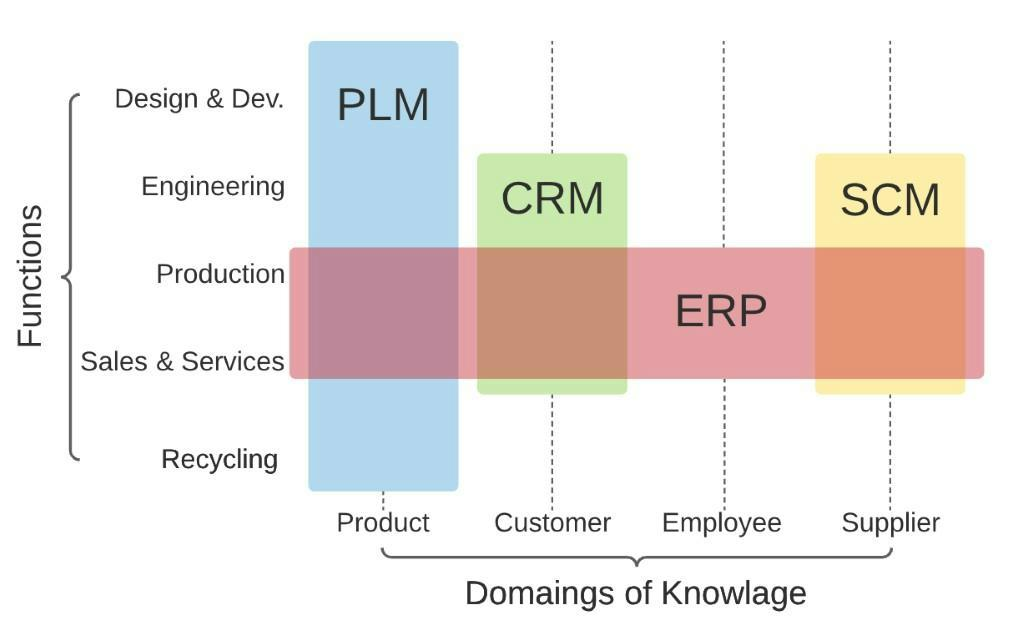
\includegraphics[width=441.67pt,height=266.95pt]{latexImage_1eeb01263024f08e27a29edca7e7a266.png}}
\end{picture}
\newpage
\begin{tikzpicture}[overlay]\path(0pt,0pt);\end{tikzpicture}
\begin{picture}(-5,0)(2.5,0)
\put(506.14,-727.616){\fontsize{12}{1}\usefont{T1}{ptm}{m}{n}\selectfont\color{color_29791}7}
\put(512.14,-727.616){\fontsize{12}{1}\usefont{T1}{ptm}{m}{n}\selectfont\color{color_29791} }
\put(515.14,-727.616){\fontsize{12}{1}\usefont{T1}{ptm}{m}{n}\selectfont\color{color_29791} }
\put(70.104,-742.496){\fontsize{10.56}{1}\usefont{T1}{ptm}{m}{n}\selectfont\color{color_29791} }
\put(72.744,-742.496){\fontsize{12}{1}\usefont{T1}{ptm}{m}{n}\selectfont\color{color_29791} }
\put(82.944,-72.34003){\fontsize{12}{1}\usefont{T1}{ptm}{m}{n}\selectfont\color{color_29791}這種跨域的廣泛覆蓋是有道理的}
\put(250.97,-72.34003){\fontsize{12}{1}\usefont{T1}{ptm}{m}{n}\selectfont\color{color_29791},}
\put(262.97,-72.34003){\fontsize{12}{1}\usefont{T1}{ptm}{m}{n}\selectfont\color{color_29791}因為}
\put(286.97,-72.34003){\fontsize{12}{1}\usefont{T1}{ptm}{m}{n}\selectfont\color{color_29791} }
\put(334.63,-72.34003){\fontsize{12}{1}\usefont{T1}{ptm}{m}{n}\selectfont\color{color_29791}ERP}
\put(356.23,-72.34003){\fontsize{12}{1}\usefont{T1}{ptm}{m}{n}\selectfont\color{color_29791} }
\put(403.87,-72.34003){\fontsize{12}{1}\usefont{T1}{ptm}{m}{n}\selectfont\color{color_29791}操作與}
\put(439.87,-72.34003){\fontsize{12}{1}\usefont{T1}{ptm}{m}{n}\selectfont\color{color_29791} }
\put(487.54,-72.34003){\fontsize{12}{1}\usefont{T1}{ptm}{m}{n}\selectfont\color{color_29791}MR}
\put(506.248,-72.34003){\fontsize{12}{1}\usefont{T1}{ptm}{m}{n}\selectfont\color{color_29791}P}
\put(512.488,-72.34003){\fontsize{12}{1}\usefont{T1}{ptm}{m}{n}\selectfont\color{color_29791} }
\put(69.384,-89.97998){\fontsize{12}{1}\usefont{T1}{ptm}{m}{n}\selectfont\color{color_29791}一樣}
\put(93.38,-89.97998){\fontsize{12}{1}\usefont{T1}{ptm}{m}{n}\selectfont\color{color_29791},}
\put(105.38,-89.97998){\fontsize{12}{1}\usefont{T1}{ptm}{m}{n}\selectfont\color{color_29791}專注於處理交易和訂單}
\put(225.41,-89.97998){\fontsize{12}{1}\usefont{T1}{ptm}{m}{n}\selectfont\color{color_29791}。}
\put(237.41,-89.97998){\fontsize{12}{1}\usefont{T1}{ptm}{m}{n}\selectfont\color{color_29791}ERP}
\put(259.49,-89.97998){\fontsize{12}{1}\usefont{T1}{ptm}{m}{n}\selectfont\color{color_29791}的重點是}
\put(307.37,-89.97998){\fontsize{12}{1}\usefont{T1}{ptm}{m}{n}\selectfont\color{color_29791}控制公司資源的輸入}
\put(415.39,-89.97998){\fontsize{12}{1}\usefont{T1}{ptm}{m}{n}\selectfont\color{color_29791}、}
\put(427.39,-89.97998){\fontsize{12}{1}\usefont{T1}{ptm}{m}{n}\selectfont\color{color_29791}保留和輸出的變}
\put(69.384,-107.74){\fontsize{12}{1}\usefont{T1}{ptm}{m}{n}\selectfont\color{color_29791}化}
\put(81.384,-107.74){\fontsize{12}{1}\usefont{T1}{ptm}{m}{n}\selectfont\color{color_29791},}
\put(93.38,-107.74){\fontsize{12}{1}\usefont{T1}{ptm}{m}{n}\selectfont\color{color_29791}無論是產品}
\put(153.38,-107.74){\fontsize{12}{1}\usefont{T1}{ptm}{m}{n}\selectfont\color{color_29791}、}
\put(165.38,-107.74){\fontsize{12}{1}\usefont{T1}{ptm}{m}{n}\selectfont\color{color_29791}原材料還是包裝}
\put(249.41,-107.74){\fontsize{12}{1}\usefont{T1}{ptm}{m}{n}\selectfont\color{color_29791}。}
\put(261.41,-107.74){\fontsize{12}{1}\usefont{T1}{ptm}{m}{n}\selectfont\color{color_29791} }
\put(264.41,-107.74){\fontsize{12}{1}\usefont{T1}{ptm}{m}{n}\selectfont\color{color_29791} }
\put(84.264,-125.14){\fontsize{12}{1}\usefont{T1}{ptm}{m}{n}\selectfont\color{color_29791} }
\put(87.26,-125.14){\fontsize{12}{1}\usefont{T1}{ptm}{m}{n}\selectfont\color{color_29791} }
\put(82.944,-141.1){\fontsize{12}{1}\usefont{T1}{ptm}{m}{n}\selectfont\color{color_29791}從同一張圖片中}
\put(166.94,-141.1){\fontsize{12}{1}\usefont{T1}{ptm}{m}{n}\selectfont\color{color_29791},}
\put(178.94,-141.1){\fontsize{12}{1}\usefont{T1}{ptm}{m}{n}\selectfont\color{color_29791}可以看出}
\put(226.97,-141.1){\fontsize{12}{1}\usefont{T1}{ptm}{m}{n}\selectfont\color{color_29791}P}
\put(233.798,-141.1){\fontsize{12}{1}\usefont{T1}{ptm}{m}{n}\selectfont\color{color_29791}L}
\put(240.878,-141.1){\fontsize{12}{1}\usefont{T1}{ptm}{m}{n}\selectfont\color{color_29791}M}
\put(251.57,-141.1){\fontsize{12}{1}\usefont{T1}{ptm}{m}{n}\selectfont\color{color_29791}和}
\put(263.57,-141.1){\fontsize{12}{1}\usefont{T1}{ptm}{m}{n}\selectfont\color{color_29791}ERP}
\put(285.65,-141.1){\fontsize{12}{1}\usefont{T1}{ptm}{m}{n}\selectfont\color{color_29791}之間的理論對比}
\put(369.67,-141.1){\fontsize{12}{1}\usefont{T1}{ptm}{m}{n}\selectfont\color{color_29791},}
\put(381.67,-141.1){\fontsize{12}{1}\usefont{T1}{ptm}{m}{n}\selectfont\color{color_29791}儘管它們都非常廣泛}
\put(489.7,-141.1){\fontsize{12}{1}\usefont{T1}{ptm}{m}{n}\selectfont\color{color_29791}。}
\put(501.7,-141.1){\fontsize{12}{1}\usefont{T1}{ptm}{m}{n}\selectfont\color{color_29791}E}
\put(69.384,-158.74){\fontsize{12}{1}\usefont{T1}{ptm}{m}{n}\selectfont\color{color_29791}RP}
\put(84.144,-158.74){\fontsize{12}{1}\usefont{T1}{ptm}{m}{n}\selectfont\color{color_29791}擴展到知識領域}
\put(168.14,-158.74){\fontsize{12}{1}\usefont{T1}{ptm}{m}{n}\selectfont\color{color_29791},}
\put(180.17,-158.74){\fontsize{12}{1}\usefont{T1}{ptm}{m}{n}\selectfont\color{color_29791}但}
\put(192.05,-158.74){\fontsize{12}{1}\usefont{T1}{ptm}{m}{n}\selectfont\color{color_29791}僅限於少數功能}
\put(276.05,-158.74){\fontsize{12}{1}\usefont{T1}{ptm}{m}{n}\selectfont\color{color_29791},}
\put(288.05,-158.74){\fontsize{12}{1}\usefont{T1}{ptm}{m}{n}\selectfont\color{color_29791}而}
\put(300.05,-158.74){\fontsize{12}{1}\usefont{T1}{ptm}{m}{n}\selectfont\color{color_29791}P}
\put(306.878,-158.74){\fontsize{12}{1}\usefont{T1}{ptm}{m}{n}\selectfont\color{color_29791}L}
\put(314.078,-158.74){\fontsize{12}{1}\usefont{T1}{ptm}{m}{n}\selectfont\color{color_29791}M}
\put(324.79,-158.74){\fontsize{12}{1}\usefont{T1}{ptm}{m}{n}\selectfont\color{color_29791}則擴展到涉及產品的所有功能}
\put(480.82,-158.74){\fontsize{12}{1}\usefont{T1}{ptm}{m}{n}\selectfont\color{color_29791}。}
\put(492.82,-158.74){\fontsize{12}{1}\usefont{T1}{ptm}{m}{n}\selectfont\color{color_29791}如}
\put(69.384,-176.38){\fontsize{12}{1}\usefont{T1}{ptm}{m}{n}\selectfont\color{color_29791}圖}
\put(81.384,-176.38){\fontsize{12}{1}\usefont{T1}{ptm}{m}{n}\selectfont\color{color_29791} }
\put(101.9,-176.38){\fontsize{12}{1}\usefont{T1}{ptm}{m}{n}\selectfont\color{color_29791}3 }
\put(128.42,-176.38){\fontsize{12}{1}\usefont{T1}{ptm}{m}{n}\selectfont\color{color_29791}所示}
\put(152.42,-176.38){\fontsize{12}{1}\usefont{T1}{ptm}{m}{n}\selectfont\color{color_29791},}
\put(164.42,-176.38){\fontsize{12}{1}\usefont{T1}{ptm}{m}{n}\selectfont\color{color_29791}代表}
\put(188.528,-176.38){\fontsize{12}{1}\usefont{T1}{ptm}{m}{n}\selectfont\color{color_29791}兩者之間良好差異的另一個觀點是}
\put(368.59,-176.38){\fontsize{12}{1}\usefont{T1}{ptm}{m}{n}\selectfont\color{color_29791},}
\put(380.59,-176.38){\fontsize{12}{1}\usefont{T1}{ptm}{m}{n}\selectfont\color{color_29791}在}
\put(392.59,-176.38){\fontsize{12}{1}\usefont{T1}{ptm}{m}{n}\selectfont\color{color_29791} }
\put(413.11,-176.38){\fontsize{12}{1}\usefont{T1}{ptm}{m}{n}\selectfont\color{color_29791}ERP}
\put(434.71,-176.38){\fontsize{12}{1}\usefont{T1}{ptm}{m}{n}\selectfont\color{color_29791} }
\put(455.26,-176.38){\fontsize{12}{1}\usefont{T1}{ptm}{m}{n}\selectfont\color{color_29791}和}
\put(467.26,-176.38){\fontsize{12}{1}\usefont{T1}{ptm}{m}{n}\selectfont\color{color_29791} }
\put(487.78,-176.38){\fontsize{12}{1}\usefont{T1}{ptm}{m}{n}\selectfont\color{color_29791}P}
\put(494.608,-176.38){\fontsize{12}{1}\usefont{T1}{ptm}{m}{n}\selectfont\color{color_29791}L}
\put(501.688,-176.38){\fontsize{12}{1}\usefont{T1}{ptm}{m}{n}\selectfont\color{color_29791}M}
\put(512.476,-176.38){\fontsize{12}{1}\usefont{T1}{ptm}{m}{n}\selectfont\color{color_29791} }
\put(69.384,-194.14){\fontsize{12}{1}\usefont{T1}{ptm}{m}{n}\selectfont\color{color_29791}影響行業的規模或詳細程度}
\put(213.41,-194.14){\fontsize{12}{1}\usefont{T1}{ptm}{m}{n}\selectfont\color{color_29791}(}
\put(225.41,-194.14){\fontsize{12}{1}\usefont{T1}{ptm}{m}{n}\selectfont\color{color_29791}即兩個系統的粒度}
\put(321.43,-194.14){\fontsize{12}{1}\usefont{T1}{ptm}{m}{n}\selectfont\color{color_29791})}
\put(333.43,-194.14){\fontsize{12}{1}\usefont{T1}{ptm}{m}{n}\selectfont\color{color_29791}方面缺乏重疊}
\put(405.43,-194.14){\fontsize{12}{1}\usefont{T1}{ptm}{m}{n}\selectfont\color{color_29791}。}
\put(417.43,-194.14){\fontsize{12}{1}\usefont{T1}{ptm}{m}{n}\selectfont\color{color_29791}  }
\put(423.43,-194.14){\fontsize{12}{1}\usefont{T1}{ptm}{m}{n}\selectfont\color{color_29791} }
\put(70.104,-211.54){\fontsize{11.04}{1}\usefont{T1}{uarial}{m}{n}\selectfont\color{color_137925} }
\put(73.104,-211.54){\fontsize{12}{1}\usefont{T1}{ptm}{m}{n}\selectfont\color{color_29791} }
\put(70.104,-227.26){\fontsize{11.04}{1}\usefont{T1}{uarial}{m}{n}\selectfont\color{color_137925}  }
\put(76.224,-227.26){\fontsize{12}{1}\usefont{T1}{ptm}{m}{n}\selectfont\color{color_29791} }
\put(425.59,-442.59){\fontsize{12}{1}\usefont{T1}{ptm}{m}{n}\selectfont\color{color_29791} }
\put(428.59,-442.59){\fontsize{12}{1}\usefont{T1}{ptm}{m}{n}\selectfont\color{color_29791} }
\put(122.18,-455.07){\fontsize{12}{1}\usefont{T1}{ptm}{m}{n}\selectfont\color{color_29791}圖}
\put(134.3,-455.07){\fontsize{12}{1}\usefont{T1}{ptm}{b}{n}\selectfont\color{color_29791}3 }
\put(143.3,-455.07){\fontsize{12}{1}\usefont{T1}{ptm}{b}{n}\selectfont\color{color_29791}E}
\put(151.328,-455.07){\fontsize{12}{1}\usefont{T1}{ptm}{b}{n}\selectfont\color{color_29791}RP}
\put(167.18,-455.07){\fontsize{12}{1}\usefont{T1}{ptm}{m}{n}\selectfont\color{color_29791}和}
\put(179.3,-455.07){\fontsize{12}{1}\usefont{T1}{ptm}{b}{n}\selectfont\color{color_29791}P}
\put(186.5,-455.07){\fontsize{12}{1}\usefont{T1}{ptm}{b}{n}\selectfont\color{color_29791}L}
\put(194.528,-455.07){\fontsize{12}{1}\usefont{T1}{ptm}{b}{n}\selectfont\color{color_29791}M}
\put(205.85,-455.07){\fontsize{12}{1}\usefont{T1}{ptm}{m}{n}\selectfont\color{color_29791}在}
\put(217.958,-455.07){\fontsize{12}{1}\usefont{T1}{ptm}{m}{n}\selectfont\color{color_29791}粒度方面的可}
\put(290.066,-455.07){\fontsize{12}{1}\usefont{T1}{ptm}{m}{n}\selectfont\color{color_29791}視化比較}
\put(338.11,-455.07){\fontsize{12}{1}\usefont{T1}{ptm}{m}{n}\selectfont\color{color_29791}(}
\put(350.11,-455.07){\fontsize{12}{1}\usefont{T1}{ptm}{m}{n}\selectfont\color{color_29791}改編自}
\put(386.23,-455.07){\fontsize{12}{1}\usefont{T1}{ptm}{b}{n}\selectfont\color{color_29791}S}
\put(392.938,-455.07){\fontsize{12}{1}\usefont{T1}{ptm}{b}{n}\selectfont\color{color_29791}tar}
\put(408.178,-455.07){\fontsize{12}{1}\usefont{T1}{ptm}{b}{n}\selectfont\color{color_29791}k}
\put(414.79,-455.07){\fontsize{12}{1}\usefont{T1}{ptm}{m}{n}\selectfont\color{color_29791},}
\put(426.91,-455.07){\fontsize{12}{1}\usefont{T1}{ptm}{b}{n}\selectfont\color{color_29791}2015}
\put(450.82,-455.07){\fontsize{12}{1}\usefont{T1}{ptm}{m}{n}\selectfont\color{color_29791})}
\put(462.94,-455.07){\fontsize{12}{1}\usefont{T1}{ptm}{b}{n}\selectfont\color{color_29791} }
\put(465.82,-455.07){\fontsize{12}{1}\usefont{T1}{ptm}{m}{n}\selectfont\color{color_29791} }
\put(70.104,-472.35){\fontsize{11.04}{1}\usefont{T1}{uarial}{m}{n}\selectfont\color{color_137925} }
\put(73.104,-472.35){\fontsize{12}{1}\usefont{T1}{ptm}{m}{n}\selectfont\color{color_29791} }
\put(82.944,-489.15){\fontsize{12}{1}\usefont{T1}{ptm}{m}{n}\selectfont\color{color_29791}正如我們所看到的}
\put(178.94,-489.15){\fontsize{12}{1}\usefont{T1}{ptm}{m}{n}\selectfont\color{color_29791},}
\put(190.97,-489.15){\fontsize{12}{1}\usefont{T1}{ptm}{m}{n}\selectfont\color{color_29791}ERP}
\put(213.05,-489.15){\fontsize{12}{1}\usefont{T1}{ptm}{m}{n}\selectfont\color{color_29791}主要關注交易和訂單}
\put(320.95,-489.15){\fontsize{12}{1}\usefont{T1}{ptm}{m}{n}\selectfont\color{color_29791}。}
\put(332.95,-489.15){\fontsize{12}{1}\usefont{T1}{ptm}{m}{n}\selectfont\color{color_29791}一旦訂單被關閉}
\put(416.95,-489.15){\fontsize{12}{1}\usefont{T1}{ptm}{m}{n}\selectfont\color{color_29791},}
\put(428.95,-489.15){\fontsize{12}{1}\usefont{T1}{ptm}{m}{n}\selectfont\color{color_29791}ERP}
\put(451.06,-489.15){\fontsize{12}{1}\usefont{T1}{ptm}{m}{n}\selectfont\color{color_29791}系統就會處}
\put(69.384,-506.79){\fontsize{12}{1}\usefont{T1}{ptm}{m}{n}\selectfont\color{color_29791}理與該訂單相關的交易}
\put(189.41,-506.79){\fontsize{12}{1}\usefont{T1}{ptm}{m}{n}\selectfont\color{color_29791},}
\put(201.41,-506.79){\fontsize{12}{1}\usefont{T1}{ptm}{m}{n}\selectfont\color{color_29791}但不太關心超出該訂單的訂單}
\put(357.43,-506.79){\fontsize{12}{1}\usefont{T1}{ptm}{m}{n}\selectfont\color{color_29791}。}
\put(369.43,-506.79){\fontsize{12}{1}\usefont{T1}{ptm}{m}{n}\selectfont\color{color_29791}另一方面}
\put(417.43,-506.79){\fontsize{12}{1}\usefont{T1}{ptm}{m}{n}\selectfont\color{color_29791},}
\put(429.43,-506.79){\fontsize{12}{1}\usefont{T1}{ptm}{m}{n}\selectfont\color{color_29791}P}
\put(436.258,-506.79){\fontsize{12}{1}\usefont{T1}{ptm}{m}{n}\selectfont\color{color_29791}L}
\put(443.338,-506.79){\fontsize{12}{1}\usefont{T1}{ptm}{m}{n}\selectfont\color{color_29791}M}
\put(454.06,-506.79){\fontsize{12}{1}\usefont{T1}{ptm}{m}{n}\selectfont\color{color_29791}的粒度與}
\put(69.384,-524.43){\fontsize{12}{1}\usefont{T1}{ptm}{m}{n}\selectfont\color{color_29791}產品的訂單有關}
\put(153.38,-524.43){\fontsize{12}{1}\usefont{T1}{ptm}{m}{n}\selectfont\color{color_29791},}
\put(165.38,-524.43){\fontsize{12}{1}\usefont{T1}{ptm}{m}{n}\selectfont\color{color_29791}不僅延伸到程式中}
\put(261.41,-524.43){\fontsize{12}{1}\usefont{T1}{ptm}{m}{n}\selectfont\color{color_29791},}
\put(273.41,-524.43){\fontsize{12}{1}\usefont{T1}{ptm}{m}{n}\selectfont\color{color_29791}還延伸到家庭和整個行業}
\put(405.43,-524.43){\fontsize{12}{1}\usefont{T1}{ptm}{m}{n}\selectfont\color{color_29791}(}
\put(417.43,-524.43){\fontsize{12}{1}\usefont{T1}{ptm}{m}{n}\selectfont\color{color_29791}S}
\put(424.138,-524.43){\fontsize{12}{1}\usefont{T1}{ptm}{m}{n}\selectfont\color{color_29791}t}
\put(427.378,-524.43){\fontsize{12}{1}\usefont{T1}{ptm}{m}{n}\selectfont\color{color_29791}a}
\put(432.658,-524.43){\fontsize{12}{1}\usefont{T1}{ptm}{m}{n}\selectfont\color{color_29791}rk}
\put(442.63,-524.43){\fontsize{12}{1}\usefont{T1}{ptm}{m}{n}\selectfont\color{color_29791},}
\put(454.66,-524.43){\fontsize{12}{1}\usefont{T1}{ptm}{m}{n}\selectfont\color{color_29791}2015}
\put(478.66,-524.43){\fontsize{12}{1}\usefont{T1}{ptm}{m}{n}\selectfont\color{color_29791})。}
\put(502.66,-524.43){\fontsize{12}{1}\usefont{T1}{ptm}{m}{n}\selectfont\color{color_29791} }
\put(505.78,-524.43){\fontsize{12}{1}\usefont{T1}{ptm}{m}{n}\selectfont\color{color_29791} }
\put(84.264,-541.95){\fontsize{12}{1}\usefont{T1}{ptm}{m}{n}\selectfont\color{color_29791} }
\put(87.26,-541.95){\fontsize{12}{1}\usefont{T1}{ptm}{m}{n}\selectfont\color{color_29791} }
\put(82.944,-558.03){\fontsize{12}{1}\usefont{T1}{ptm}{m}{n}\selectfont\color{color_29791}這特別有趣}
\put(142.94,-558.03){\fontsize{12}{1}\usefont{T1}{ptm}{m}{n}\selectfont\color{color_29791},}
\put(154.94,-558.03){\fontsize{12}{1}\usefont{T1}{ptm}{m}{n}\selectfont\color{color_29791}因為它展示了這兩個系統如何能夠並且確實在現場相互補充}
\put(467.02,-558.03){\fontsize{12}{1}\usefont{T1}{ptm}{m}{n}\selectfont\color{color_29791}。}
\put(479.02,-558.03){\fontsize{12}{1}\usefont{T1}{ptm}{m}{n}\selectfont\color{color_29791}ERP}
\put(69.384,-575.67){\fontsize{12}{1}\usefont{T1}{ptm}{m}{n}\selectfont\color{color_29791}應該指出的一個方面是}
\put(189.41,-575.67){\fontsize{12}{1}\usefont{T1}{ptm}{m}{n}\selectfont\color{color_29791},}
\put(201.41,-575.67){\fontsize{12}{1}\usefont{T1}{ptm}{m}{n}\selectfont\color{color_29791}它與其他系統集成相對容易}
\put(345.43,-575.67){\fontsize{12}{1}\usefont{T1}{ptm}{m}{n}\selectfont\color{color_29791}。}
\put(357.43,-575.67){\fontsize{12}{1}\usefont{T1}{ptm}{m}{n}\selectfont\color{color_29791}例如}
\put(381.43,-575.67){\fontsize{12}{1}\usefont{T1}{ptm}{m}{n}\selectfont\color{color_29791},}
\put(393.43,-575.67){\fontsize{12}{1}\usefont{T1}{ptm}{m}{n}\selectfont\color{color_29791}ERP}
\put(415.51,-575.67){\fontsize{12}{1}\usefont{T1}{ptm}{m}{n}\selectfont\color{color_29791}-}
\put(69.384,-593.34){\fontsize{12}{1}\usefont{T1}{ptm}{m}{n}\selectfont\color{color_29791}MES}
\put(94.1,-593.34){\fontsize{12}{1}\usefont{T1}{ptm}{m}{n}\selectfont\color{color_29791}集成已被廣泛研究和實施}
\put(226.13,-593.34){\fontsize{12}{1}\usefont{T1}{ptm}{m}{n}\selectfont\color{color_29791},}
\put(238.13,-593.34){\fontsize{12}{1}\usefont{T1}{ptm}{m}{n}\selectfont\color{color_29791}並已為其制定了標準}
\put(346.15,-593.34){\fontsize{12}{1}\usefont{T1}{ptm}{m}{n}\selectfont\color{color_29791}(}
\put(358.27,-593.34){\fontsize{12}{1}\usefont{T1}{ptm}{m}{n}\selectfont\color{color_29791}I}
\put(361.99,-593.34){\fontsize{12}{1}\usefont{T1}{ptm}{m}{n}\selectfont\color{color_29791}S}
\put(368.818,-593.34){\fontsize{12}{1}\usefont{T1}{ptm}{m}{n}\selectfont\color{color_29791}A}
\put(376.738,-593.34){\fontsize{12}{1}\usefont{T1}{ptm}{m}{n}\selectfont\color{color_29791} }
\put(410.206,-593.34){\fontsize{12}{1}\usefont{T1}{ptm}{m}{n}\selectfont\color{color_29791}95}
\put(422.314,-593.34){\fontsize{12}{1}\usefont{T1}{ptm}{m}{n}\selectfont\color{color_29791} }
\put(455.86,-593.34){\fontsize{12}{1}\usefont{T1}{ptm}{m}{n}\selectfont\color{color_29791}-}
\put(459.82,-593.34){\fontsize{12}{1}\usefont{T1}{ptm}{m}{n}\selectfont\color{color_29791} }
\put(493.42,-593.34){\fontsize{12}{1}\usefont{T1}{ptm}{m}{n}\selectfont\color{color_29791}I}
\put(497.26,-593.34){\fontsize{12}{1}\usefont{T1}{ptm}{m}{n}\selectfont\color{color_29791}EC}
\put(512.5,-593.34){\fontsize{12}{1}\usefont{T1}{ptm}{m}{n}\selectfont\color{color_29791} }
\put(69.384,-610.98){\fontsize{12}{1}\usefont{T1}{ptm}{m}{n}\selectfont\color{color_29791}62264}
\put(99.38,-610.98){\fontsize{12}{1}\usefont{T1}{ptm}{m}{n}\selectfont\color{color_29791})。}
\put(123.38,-610.98){\fontsize{12}{1}\usefont{T1}{ptm}{m}{n}\selectfont\color{color_29791}其中一個論點是}
\put(207.41,-610.98){\fontsize{12}{1}\usefont{T1}{ptm}{m}{n}\selectfont\color{color_29791}ERP}
\put(229.49,-610.98){\fontsize{12}{1}\usefont{T1}{ptm}{m}{n}\selectfont\color{color_29791}系統的模組化}
\put(301.37,-610.98){\fontsize{12}{1}\usefont{T1}{ptm}{m}{n}\selectfont\color{color_29791}性質}
\put(325.39,-610.98){\fontsize{12}{1}\usefont{T1}{ptm}{m}{n}\selectfont\color{color_29791},}
\put(337.39,-610.98){\fontsize{12}{1}\usefont{T1}{ptm}{m}{n}\selectfont\color{color_29791}在論文}
\put(373.39,-610.98){\fontsize{12}{1}\usefont{T1}{ptm}{m}{n}\selectfont\color{color_29791}(}
\put(385.39,-610.98){\fontsize{12}{1}\usefont{T1}{ptm}{m}{n}\selectfont\color{color_29791}第}
\put(397.39,-610.98){\fontsize{12}{1}\usefont{T1}{ptm}{m}{n}\selectfont\color{color_29791}5}
\put(403.39,-610.98){\fontsize{12}{1}\usefont{T1}{ptm}{m}{n}\selectfont\color{color_29791}章}
\put(415.39,-610.98){\fontsize{12}{1}\usefont{T1}{ptm}{m}{n}\selectfont\color{color_29791})}
\put(427.39,-610.98){\fontsize{12}{1}\usefont{T1}{ptm}{m}{n}\selectfont\color{color_29791}中進一步討論了}
\put(69.384,-628.62){\fontsize{12}{1}\usefont{T1}{ptm}{m}{n}\selectfont\color{color_29791}Odoo}
\put(96.02,-628.62){\fontsize{12}{1}\usefont{T1}{ptm}{m}{n}\selectfont\color{color_29791}軟體}
\put(120.02,-628.62){\fontsize{12}{1}\usefont{T1}{ptm}{m}{n}\selectfont\color{color_29791}。}
\put(132.02,-628.62){\fontsize{12}{1}\usefont{T1}{ptm}{m}{n}\selectfont\color{color_29791}這是因為}
\put(180.05,-628.62){\fontsize{12}{1}\usefont{T1}{ptm}{m}{n}\selectfont\color{color_29791}O}
\put(188.798,-628.62){\fontsize{12}{1}\usefont{T1}{ptm}{m}{n}\selectfont\color{color_29791}doo}
\put(206.81,-628.62){\fontsize{12}{1}\usefont{T1}{ptm}{m}{n}\selectfont\color{color_29791}軟體最初是從開源}
\put(302.81,-628.62){\fontsize{12}{1}\usefont{T1}{ptm}{m}{n}\selectfont\color{color_29791}ERP}
\put(324.91,-628.62){\fontsize{12}{1}\usefont{T1}{ptm}{m}{n}\selectfont\color{color_29791}系統演變而來的}
\put(408.91,-628.62){\fontsize{12}{1}\usefont{T1}{ptm}{m}{n}\selectfont\color{color_29791}。}
\put(420.91,-628.62){\fontsize{12}{1}\usefont{T1}{ptm}{m}{n}\selectfont\color{color_29791} }
\put(423.79,-628.62){\fontsize{12}{1}\usefont{T1}{ptm}{m}{n}\selectfont\color{color_29791} }
\put(70.104,-646.14){\fontsize{11.04}{1}\usefont{T1}{uarial}{m}{n}\selectfont\color{color_29791} }
\put(73.104,-646.14){\fontsize{12}{1}\usefont{T1}{ptm}{m}{n}\selectfont\color{color_29791} }
\put(82.944,-663.06){\fontsize{12}{1}\usefont{T1}{ptm}{m}{n}\selectfont\color{color_29791}ERP}
\put(105.02,-663.06){\fontsize{12}{1}\usefont{T1}{ptm}{m}{n}\selectfont\color{color_29791}系統的本質最好地}
\put(200.9,-663.06){\fontsize{12}{1}\usefont{T1}{ptm}{m}{n}\selectfont\color{color_29791}總結為}
\put(236.93,-663.06){\fontsize{12}{1}\usefont{T1}{ptm}{m}{n}\selectfont\color{color_29791}(}
\put(248.93,-663.06){\fontsize{12}{1}\usefont{T1}{ptm}{m}{n}\selectfont\color{color_29791}Umble }
\put(386.822,-663.06){\fontsize{12}{1}\usefont{T1}{ptm}{m}{n}\selectfont\color{color_29791}e}
\put(392.102,-663.06){\fontsize{12}{1}\usefont{T1}{ptm}{m}{n}\selectfont\color{color_29791}t }
\put(500.714,-663.06){\fontsize{12}{1}\usefont{T1}{ptm}{m}{n}\selectfont\color{color_29791}a}
\put(505.994,-663.06){\fontsize{12}{1}\usefont{T1}{ptm}{m}{n}\selectfont\color{color_29791}l.}
\put(512.462,-663.06){\fontsize{12}{1}\usefont{T1}{ptm}{m}{n}\selectfont\color{color_29791} }
\put(69.384,-680.7){\fontsize{12}{1}\usefont{T1}{ptm}{m}{n}\selectfont\color{color_29791}2003}
\put(93.38,-680.7){\fontsize{12}{1}\usefont{T1}{ptm}{m}{n}\selectfont\color{color_29791}):}
\put(117.38,-680.7){\fontsize{12}{1}\usefont{T1}{ptm}{m}{n}\selectfont\color{color_29791}ERP}
\put(139.46,-680.7){\fontsize{12}{1}\usefont{T1}{ptm}{m}{n}\selectfont\color{color_29791}提供了一}
\put(187.34,-680.7){\fontsize{12}{1}\usefont{T1}{ptm}{m}{n}\selectfont\color{color_29791}個統一的企業業務視圖}
\put(307.37,-680.7){\fontsize{12}{1}\usefont{T1}{ptm}{m}{n}\selectfont\color{color_29791},}
\put(319.39,-680.7){\fontsize{12}{1}\usefont{T1}{ptm}{m}{n}\selectfont\color{color_29791}包括所有職能和部門}
\put(427.39,-680.7){\fontsize{12}{1}\usefont{T1}{ptm}{m}{n}\selectfont\color{color_29791},}
\put(439.39,-680.7){\fontsize{12}{1}\usefont{T1}{ptm}{m}{n}\selectfont\color{color_29791}以及一個企業}
\put(69.384,-698.216){\fontsize{12}{1}\usefont{T1}{ptm}{m}{n}\selectfont\color{color_29791}資料庫}
\put(105.38,-698.216){\fontsize{12}{1}\usefont{T1}{ptm}{m}{n}\selectfont\color{color_29791},}
\put(117.38,-698.216){\fontsize{12}{1}\usefont{T1}{ptm}{m}{n}\selectfont\color{color_29791}其中跟蹤了與財務}
\put(213.41,-698.216){\fontsize{12}{1}\usefont{T1}{ptm}{m}{n}\selectfont\color{color_29791}、}
\put(225.41,-698.216){\fontsize{12}{1}\usefont{T1}{ptm}{m}{n}\selectfont\color{color_29791}銷售}
\put(249.41,-698.216){\fontsize{12}{1}\usefont{T1}{ptm}{m}{n}\selectfont\color{color_29791}、}
\put(261.41,-698.216){\fontsize{12}{1}\usefont{T1}{ptm}{m}{n}\selectfont\color{color_29791}營銷}
\put(285.41,-698.216){\fontsize{12}{1}\usefont{T1}{ptm}{m}{n}\selectfont\color{color_29791}、}
\put(297.41,-698.216){\fontsize{12}{1}\usefont{T1}{ptm}{m}{n}\selectfont\color{color_29791}採購和人力資源有關的所有行動}
\put(465.46,-698.216){\fontsize{12}{1}\usefont{T1}{ptm}{m}{n}\selectfont\color{color_29791}。}
\put(477.46,-698.216){\fontsize{12}{1}\usefont{T1}{ptm}{m}{n}\selectfont\color{color_29791}實現}
\put(156.4,-442.45){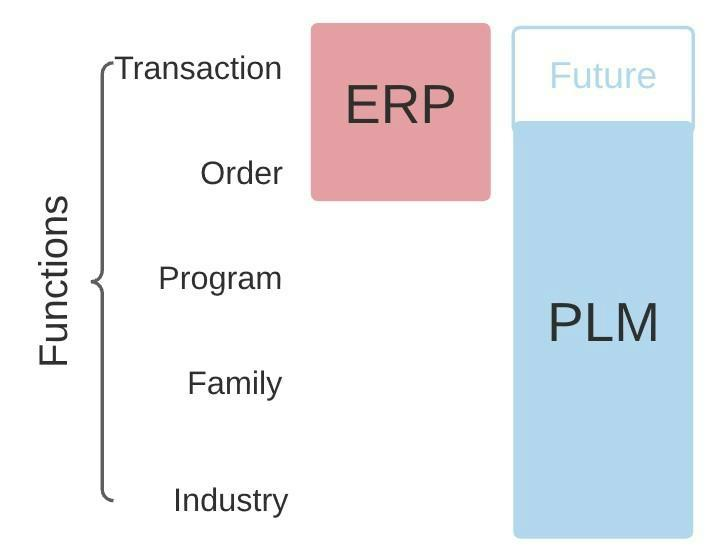
\includegraphics[width=269.25pt,height=211.5pt]{latexImage_e6a13fafc3da5cca07c057a89d16b34b.png}}
\end{picture}
\newpage
\begin{tikzpicture}[overlay]\path(0pt,0pt);\end{tikzpicture}
\begin{picture}(-5,0)(2.5,0)
\put(506.14,-727.616){\fontsize{12}{1}\usefont{T1}{ptm}{m}{n}\selectfont\color{color_29791}8}
\put(512.14,-727.616){\fontsize{12}{1}\usefont{T1}{ptm}{m}{n}\selectfont\color{color_29791} }
\put(515.14,-727.616){\fontsize{12}{1}\usefont{T1}{ptm}{m}{n}\selectfont\color{color_29791} }
\put(70.104,-742.496){\fontsize{10.56}{1}\usefont{T1}{ptm}{m}{n}\selectfont\color{color_29791} }
\put(72.744,-742.496){\fontsize{12}{1}\usefont{T1}{ptm}{m}{n}\selectfont\color{color_29791} }
\put(69.384,-72.34003){\fontsize{12}{1}\usefont{T1}{ptm}{m}{n}\selectfont\color{color_29791}這一目標的目的是擴大客戶目標}
\put(237.41,-72.34003){\fontsize{12}{1}\usefont{T1}{ptm}{m}{n}\selectfont\color{color_29791},}
\put(249.41,-72.34003){\fontsize{12}{1}\usefont{T1}{ptm}{m}{n}\selectfont\color{color_29791}並在緩慢轉向創新的市場中增加客戶份額}
\put(465.46,-72.34003){\fontsize{12}{1}\usefont{T1}{ptm}{m}{n}\selectfont\color{color_29791}(}
\put(477.46,-72.34003){\fontsize{12}{1}\usefont{T1}{ptm}{m}{n}\selectfont\color{color_29791}Vá}
\put(491.38,-72.34003){\fontsize{12}{1}\usefont{T1}{ptm}{m}{n}\selectfont\color{color_29791}squ}
\put(69.384,-90.09998){\fontsize{12}{1}\usefont{T1}{ptm}{m}{n}\selectfont\color{color_29791}ez}
\put(80.064,-90.09998){\fontsize{12}{1}\usefont{T1}{ptm}{m}{n}\selectfont\color{color_29791}和}
\put(92.06,-90.09998){\fontsize{12}{1}\usefont{T1}{ptm}{m}{n}\selectfont\color{color_29791}Esc}
\put(109.34,-90.09998){\fontsize{12}{1}\usefont{T1}{ptm}{m}{n}\selectfont\color{color_29791}riba}
\put(127.94,-90.09998){\fontsize{12}{1}\usefont{T1}{ptm}{m}{n}\selectfont\color{color_29791}no}
\put(139.94,-90.09998){\fontsize{12}{1}\usefont{T1}{ptm}{m}{n}\selectfont\color{color_29791},}
\put(151.94,-90.09998){\fontsize{12}{1}\usefont{T1}{ptm}{m}{n}\selectfont\color{color_29791}2017}
\put(175.94,-90.09998){\fontsize{12}{1}\usefont{T1}{ptm}{m}{n}\selectfont\color{color_29791})。}
\put(200.09,-90.09998){\fontsize{12}{1}\usefont{T1}{ptm}{m}{n}\selectfont\color{color_29791} }
\put(203.09,-90.09998){\fontsize{12}{1}\usefont{T1}{ptm}{m}{n}\selectfont\color{color_29791} }
\put(84.264,-107.5){\fontsize{12}{1}\usefont{T1}{ptm}{m}{n}\selectfont\color{color_29791} }
\put(87.26,-107.5){\fontsize{12}{1}\usefont{T1}{ptm}{m}{n}\selectfont\color{color_29791} }
\put(87.38,-124.54){\fontsize{14.04}{1}\usefont{T1}{ptm}{b}{n}\selectfont\color{color_29791}2}
\put(94.44212,-124.54){\fontsize{14.04}{1}\usefont{T1}{ptm}{b}{n}\selectfont\color{color_29791}.3. }
\put(111.86,-124.54){\fontsize{14.04}{1}\usefont{T1}{ptm}{m}{n}\selectfont\color{color_29791}製造執行系統}
\put(196.13,-124.54){\fontsize{14.04}{1}\usefont{T1}{ptm}{b}{n}\selectfont\color{color_29791}  }
\put(202.97,-124.54){\fontsize{14.04}{1}\usefont{T1}{ptm}{b}{n}\selectfont\color{color_29791} }
\put(82.944,-159.1){\fontsize{12}{1}\usefont{T1}{ptm}{m}{n}\selectfont\color{color_29791}一個完全集成的系統的最後一個關鍵是製造執行系統}
\put(358.99,-159.1){\fontsize{12}{1}\usefont{T1}{ptm}{m}{n}\selectfont\color{color_29791}(}
\put(370.99,-159.1){\fontsize{12}{1}\usefont{T1}{ptm}{m}{n}\selectfont\color{color_29791}MES}
\put(395.71,-159.1){\fontsize{12}{1}\usefont{T1}{ptm}{m}{n}\selectfont\color{color_29791})。}
\put(419.71,-159.1){\fontsize{12}{1}\usefont{T1}{ptm}{m}{n}\selectfont\color{color_29791}MES}
\put(444.31,-159.1){\fontsize{12}{1}\usefont{T1}{ptm}{m}{n}\selectfont\color{color_29791}是管理層和}
\put(69.384,-176.74){\fontsize{12}{1}\usefont{T1}{ptm}{m}{n}\selectfont\color{color_29791}生產層之間的一層溝通}
\put(189.41,-176.74){\fontsize{12}{1}\usefont{T1}{ptm}{m}{n}\selectfont\color{color_29791};}
\put(192.77,-176.74){\fontsize{12}{1}\usefont{T1}{ptm}{m}{n}\selectfont\color{color_29791}它是一種軟體}
\put(264.77,-176.74){\fontsize{12}{1}\usefont{T1}{ptm}{m}{n}\selectfont\color{color_29791},}
\put(276.77,-176.74){\fontsize{12}{1}\usefont{T1}{ptm}{m}{n}\selectfont\color{color_29791}允許組織層面}
\put(348.79,-176.74){\fontsize{12}{1}\usefont{T1}{ptm}{m}{n}\selectfont\color{color_29791}(}
\put(360.79,-176.74){\fontsize{12}{1}\usefont{T1}{ptm}{m}{n}\selectfont\color{color_29791}通常由}
\put(396.79,-176.74){\fontsize{12}{1}\usefont{T1}{ptm}{m}{n}\selectfont\color{color_29791}ERP}
\put(418.75,-176.74){\fontsize{12}{1}\usefont{T1}{ptm}{m}{n}\selectfont\color{color_29791}支援}
\put(442.75,-176.74){\fontsize{12}{1}\usefont{T1}{ptm}{m}{n}\selectfont\color{color_29791})}
\put(454.78,-176.74){\fontsize{12}{1}\usefont{T1}{ptm}{m}{n}\selectfont\color{color_29791}與車間控}
\put(69.384,-194.38){\fontsize{12}{1}\usefont{T1}{ptm}{m}{n}\selectfont\color{color_29791}制系統}
\put(105.38,-194.38){\fontsize{12}{1}\usefont{T1}{ptm}{m}{n}\selectfont\color{color_29791}(}
\put(117.38,-194.38){\fontsize{12}{1}\usefont{T1}{ptm}{m}{n}\selectfont\color{color_29791}其中採用了幾個不同的}
\put(237.41,-194.38){\fontsize{12}{1}\usefont{T1}{ptm}{m}{n}\selectfont\color{color_29791},}
\put(249.41,-194.38){\fontsize{12}{1}\usefont{T1}{ptm}{m}{n}\selectfont\color{color_29791}非常定製的軟體應用程式}
\put(381.43,-194.38){\fontsize{12}{1}\usefont{T1}{ptm}{m}{n}\selectfont\color{color_29791})}
\put(393.43,-194.38){\fontsize{12}{1}\usefont{T1}{ptm}{m}{n}\selectfont\color{color_29791}之間的數據交換}
\put(477.46,-194.38){\fontsize{12}{1}\usefont{T1}{ptm}{m}{n}\selectfont\color{color_29791}(}
\put(489.46,-194.38){\fontsize{12}{1}\usefont{T1}{ptm}{m}{n}\selectfont\color{color_29791}Me}
\put(505.528,-194.38){\fontsize{12}{1}\usefont{T1}{ptm}{m}{n}\selectfont\color{color_29791}y}
\put(69.384,-212.14){\fontsize{12}{1}\usefont{T1}{ptm}{m}{n}\selectfont\color{color_29791}er}
\put(78.624,-212.14){\fontsize{12}{1}\usefont{T1}{ptm}{m}{n}\selectfont\color{color_29791}等人}
\put(102.62,-212.14){\fontsize{12}{1}\usefont{T1}{ptm}{m}{n}\selectfont\color{color_29791},}
\put(114.62,-212.14){\fontsize{12}{1}\usefont{T1}{ptm}{m}{n}\selectfont\color{color_29791}2009}
\put(138.62,-212.14){\fontsize{12}{1}\usefont{T1}{ptm}{m}{n}\selectfont\color{color_29791})。}
\put(162.62,-212.14){\fontsize{12}{1}\usefont{T1}{ptm}{m}{n}\selectfont\color{color_29791} }
\put(165.74,-212.14){\fontsize{12}{1}\usefont{T1}{ptm}{m}{n}\selectfont\color{color_29791} }
\put(82.944,-229.9){\fontsize{12}{1}\usefont{T1}{ptm}{m}{n}\selectfont\color{color_29791}圖}
\put(94.94,-229.9){\fontsize{12}{1}\usefont{T1}{ptm}{m}{n}\selectfont\color{color_29791} }
\put(97.94,-229.9){\fontsize{12}{1}\usefont{T1}{ptm}{m}{n}\selectfont\color{color_29791}4 }
\put(106.94,-229.9){\fontsize{12}{1}\usefont{T1}{ptm}{m}{n}\selectfont\color{color_29791}很好地描述了不同系統如何適應製造和開發範圍}
\put(358.99,-229.9){\fontsize{12}{1}\usefont{T1}{ptm}{m}{n}\selectfont\color{color_29791}。}
\put(370.99,-229.9){\fontsize{12}{1}\usefont{T1}{ptm}{m}{n}\selectfont\color{color_29791} }
\put(373.99,-229.9){\fontsize{12}{1}\usefont{T1}{ptm}{m}{n}\selectfont\color{color_29791} }
\put(70.104,-247.45){\fontsize{11.04}{1}\usefont{T1}{uarial}{m}{n}\selectfont\color{color_29791}  }
\put(76.224,-247.45){\fontsize{12}{1}\usefont{T1}{ptm}{m}{n}\selectfont\color{color_29791} }
\put(514.9,-469.35){\fontsize{12}{1}\usefont{T1}{ptm}{m}{n}\selectfont\color{color_29791} }
\put(517.9,-469.35){\fontsize{12}{1}\usefont{T1}{ptm}{m}{n}\selectfont\color{color_29791} }
\put(93.74,-481.83){\fontsize{12}{1}\usefont{T1}{ptm}{m}{n}\selectfont\color{color_29791}圖}
\put(105.86,-481.83){\fontsize{12}{1}\usefont{T1}{ptm}{b}{n}\selectfont\color{color_29791}4 }
\put(114.74,-481.83){\fontsize{12}{1}\usefont{T1}{ptm}{m}{n}\selectfont\color{color_29791}包括}
\put(138.86,-481.83){\fontsize{12}{1}\usefont{T1}{ptm}{b}{n}\selectfont\color{color_29791}M}
\put(150.14,-481.83){\fontsize{12}{1}\usefont{T1}{ptm}{b}{n}\selectfont\color{color_29791}E}
\put(158.168,-481.83){\fontsize{12}{1}\usefont{T1}{ptm}{b}{n}\selectfont\color{color_29791}S}
\put(164.78,-481.83){\fontsize{12}{1}\usefont{T1}{ptm}{m}{n}\selectfont\color{color_29791}在內的不同系統的}
\put(260.888,-481.83){\fontsize{12}{1}\usefont{T1}{ptm}{m}{n}\selectfont\color{color_29791}軋輥的可視化表示}
\put(356.95,-481.83){\fontsize{12}{1}\usefont{T1}{ptm}{m}{n}\selectfont\color{color_29791}(}
\put(368.95,-481.83){\fontsize{12}{1}\usefont{T1}{ptm}{m}{n}\selectfont\color{color_29791}改}
\put(381.058,-481.83){\fontsize{12}{1}\usefont{T1}{ptm}{m}{n}\selectfont\color{color_29791}編自}
\put(405.19,-481.83){\fontsize{12}{1}\usefont{T1}{ptm}{b}{n}\selectfont\color{color_29791} }
\put(408.19,-481.83){\fontsize{12}{1}\usefont{T1}{ptm}{b}{n}\selectfont\color{color_29791}m}
\put(418.03,-481.83){\fontsize{12}{1}\usefont{T1}{ptm}{b}{n}\selectfont\color{color_29791}e}
\put(423.31,-481.83){\fontsize{12}{1}\usefont{T1}{ptm}{b}{n}\selectfont\color{color_29791}sc}
\put(433.27,-481.83){\fontsize{12}{1}\usefont{T1}{ptm}{b}{n}\selectfont\color{color_29791}e}
\put(438.55,-481.83){\fontsize{12}{1}\usefont{T1}{ptm}{b}{n}\selectfont\color{color_29791}n}
\put(445.258,-481.83){\fontsize{12}{1}\usefont{T1}{ptm}{b}{n}\selectfont\color{color_29791}te}
\put(454.606,-481.83){\fontsize{12}{1}\usefont{T1}{ptm}{b}{n}\selectfont\color{color_29791}r}
\put(458.806,-481.83){\fontsize{12}{1}\usefont{T1}{ptm}{b}{n}\selectfont\color{color_29791}.or}
\put(473.086,-481.83){\fontsize{12}{1}\usefont{T1}{ptm}{b}{n}\selectfont\color{color_29791}g}
\put(479.14,-481.83){\fontsize{12}{1}\usefont{T1}{ptm}{m}{n}\selectfont\color{color_29791})}
\put(491.26,-481.83){\fontsize{12}{1}\usefont{T1}{ptm}{b}{n}\selectfont\color{color_29791} }
\put(494.26,-481.83){\fontsize{12}{1}\usefont{T1}{ptm}{m}{n}\selectfont\color{color_29791} }
\put(70.104,-499.23){\fontsize{12}{1}\usefont{T1}{ptm}{m}{n}\selectfont\color{color_29791} }
\put(73.104,-499.23){\fontsize{12}{1}\usefont{T1}{ptm}{m}{n}\selectfont\color{color_29791} }
\put(82.944,-515.31){\fontsize{12}{1}\usefont{T1}{ptm}{m}{n}\selectfont\color{color_29791}出於所有目的}
\put(154.94,-515.31){\fontsize{12}{1}\usefont{T1}{ptm}{m}{n}\selectfont\color{color_29791},}
\put(166.94,-515.31){\fontsize{12}{1}\usefont{T1}{ptm}{m}{n}\selectfont\color{color_29791}MES}
\put(191.69,-515.31){\fontsize{12}{1}\usefont{T1}{ptm}{m}{n}\selectfont\color{color_29791}的主要目標是提供數位和數據}
\put(347.71,-515.31){\fontsize{12}{1}\usefont{T1}{ptm}{m}{n}\selectfont\color{color_29791},}
\put(359.71,-515.31){\fontsize{12}{1}\usefont{T1}{ptm}{m}{n}\selectfont\color{color_29791}這些數位和數據最終不僅用}
\put(69.384,-532.95){\fontsize{12}{1}\usefont{T1}{ptm}{m}{n}\selectfont\color{color_29791}於確定產品的狀況和品質}
\put(201.41,-532.95){\fontsize{12}{1}\usefont{T1}{ptm}{m}{n}\selectfont\color{color_29791},}
\put(213.41,-532.95){\fontsize{12}{1}\usefont{T1}{ptm}{m}{n}\selectfont\color{color_29791}還用於確定影響生產的所有過程}
\put(381.43,-532.95){\fontsize{12}{1}\usefont{T1}{ptm}{m}{n}\selectfont\color{color_29791}。}
\put(393.43,-532.95){\fontsize{12}{1}\usefont{T1}{ptm}{m}{n}\selectfont\color{color_29791}機器}
\put(417.43,-532.95){\fontsize{12}{1}\usefont{T1}{ptm}{m}{n}\selectfont\color{color_29791}、}
\put(429.43,-532.95){\fontsize{12}{1}\usefont{T1}{ptm}{m}{n}\selectfont\color{color_29791}感測器以及與}
\put(69.384,-550.47){\fontsize{12}{1}\usefont{T1}{ptm}{m}{n}\selectfont\color{color_29791}產品接觸並提供任何類型的輸出的任何東西}
\put(297.41,-550.47){\fontsize{12}{1}\usefont{T1}{ptm}{m}{n}\selectfont\color{color_29791},}
\put(309.41,-550.47){\fontsize{12}{1}\usefont{T1}{ptm}{m}{n}\selectfont\color{color_29791}基本上都是將所述數據交給}
\put(453.46,-550.47){\fontsize{12}{1}\usefont{T1}{ptm}{m}{n}\selectfont\color{color_29791} }
\put(487.9,-550.47){\fontsize{12}{1}\usefont{T1}{ptm}{m}{n}\selectfont\color{color_29791}MES}
\put(512.5,-550.47){\fontsize{12}{1}\usefont{T1}{ptm}{m}{n}\selectfont\color{color_29791} }
\put(69.384,-568.11){\fontsize{12}{1}\usefont{T1}{ptm}{m}{n}\selectfont\color{color_29791}進行即時分類和處理}
\put(177.38,-568.11){\fontsize{12}{1}\usefont{T1}{ptm}{m}{n}\selectfont\color{color_29791}。}
\put(189.41,-568.11){\fontsize{12}{1}\usefont{T1}{ptm}{m}{n}\selectfont\color{color_29791}例如}
\put(213.41,-568.11){\fontsize{12}{1}\usefont{T1}{ptm}{m}{n}\selectfont\color{color_29791},}
\put(225.41,-568.11){\fontsize{12}{1}\usefont{T1}{ptm}{m}{n}\selectfont\color{color_29791}如果經理想知道即時生產數據或查看廢品率的圖形表}
\put(69.384,-585.87){\fontsize{12}{1}\usefont{T1}{ptm}{m}{n}\selectfont\color{color_29791}示}
\put(81.384,-585.87){\fontsize{12}{1}\usefont{T1}{ptm}{m}{n}\selectfont\color{color_29791},}
\put(93.38,-585.87){\fontsize{12}{1}\usefont{T1}{ptm}{m}{n}\selectfont\color{color_29791}則可以從}
\put(141.38,-585.87){\fontsize{12}{1}\usefont{T1}{ptm}{m}{n}\selectfont\color{color_29791}MES}
\put(166.1,-585.87){\fontsize{12}{1}\usefont{T1}{ptm}{m}{n}\selectfont\color{color_29791}軟體中獲得該數據}
\put(262.13,-585.87){\fontsize{12}{1}\usefont{T1}{ptm}{m}{n}\selectfont\color{color_29791}。}
\put(274.13,-585.87){\fontsize{12}{1}\usefont{T1}{ptm}{m}{n}\selectfont\color{color_29791}  }
\put(280.13,-585.87){\fontsize{12}{1}\usefont{T1}{ptm}{m}{n}\selectfont\color{color_29791} }
\put(84.264,-603.42){\fontsize{12}{1}\usefont{T1}{ptm}{m}{n}\selectfont\color{color_29791} }
\put(87.26,-603.42){\fontsize{12}{1}\usefont{T1}{ptm}{m}{n}\selectfont\color{color_29791} }
\put(82.944,-619.5){\fontsize{12}{1}\usefont{T1}{ptm}{m}{n}\selectfont\color{color_29791}傳統上}
\put(118.94,-619.5){\fontsize{12}{1}\usefont{T1}{ptm}{m}{n}\selectfont\color{color_29791},}
\put(130.94,-619.5){\fontsize{12}{1}\usefont{T1}{ptm}{m}{n}\selectfont\color{color_29791}管理層將根據此類信息評估工作並做出決策}
\put(358.99,-619.5){\fontsize{12}{1}\usefont{T1}{ptm}{m}{n}\selectfont\color{color_29791}。}
\put(370.99,-619.5){\fontsize{12}{1}\usefont{T1}{ptm}{m}{n}\selectfont\color{color_29791}如前所述}
\put(418.99,-619.5){\fontsize{12}{1}\usefont{T1}{ptm}{m}{n}\selectfont\color{color_29791},}
\put(430.99,-619.5){\fontsize{12}{1}\usefont{T1}{ptm}{m}{n}\selectfont\color{color_29791}這種數據收集}
\put(69.384,-637.14){\fontsize{12}{1}\usefont{T1}{ptm}{m}{n}\selectfont\color{color_29791}非常適合}
\put(117.38,-637.14){\fontsize{12}{1}\usefont{T1}{ptm}{m}{n}\selectfont\color{color_29791}ERP}
\put(139.46,-637.14){\fontsize{12}{1}\usefont{T1}{ptm}{m}{n}\selectfont\color{color_29791}的使用}
\put(175.46,-637.14){\fontsize{12}{1}\usefont{T1}{ptm}{m}{n}\selectfont\color{color_29791},}
\put(187.37,-637.14){\fontsize{12}{1}\usefont{T1}{ptm}{m}{n}\selectfont\color{color_29791}不僅因為如果輔以即時生產數據}
\put(355.39,-637.14){\fontsize{12}{1}\usefont{T1}{ptm}{m}{n}\selectfont\color{color_29791},}
\put(367.39,-637.14){\fontsize{12}{1}\usefont{T1}{ptm}{m}{n}\selectfont\color{color_29791}資源管理可以更加詳細}
\put(487.42,-637.14){\fontsize{12}{1}\usefont{T1}{ptm}{m}{n}\selectfont\color{color_29791},}
\put(499.42,-637.14){\fontsize{12}{1}\usefont{T1}{ptm}{m}{n}\selectfont\color{color_29791}還}
\put(69.384,-654.78){\fontsize{12}{1}\usefont{T1}{ptm}{m}{n}\selectfont\color{color_29791}因為}
\put(93.38,-654.78){\fontsize{12}{1}\usefont{T1}{ptm}{m}{n}\selectfont\color{color_29791}ERP}
\put(115.46,-654.78){\fontsize{12}{1}\usefont{T1}{ptm}{m}{n}\selectfont\color{color_29791}的模組化通常}
\put(187.34,-654.78){\fontsize{12}{1}\usefont{T1}{ptm}{m}{n}\selectfont\color{color_29791}意味著無}
\put(235.37,-654.78){\fontsize{12}{1}\usefont{T1}{ptm}{m}{n}\selectfont\color{color_29791}縫集成}
\put(271.37,-654.78){\fontsize{12}{1}\usefont{T1}{ptm}{m}{n}\selectfont\color{color_29791}。}
\put(283.37,-654.78){\fontsize{12}{1}\usefont{T1}{ptm}{m}{n}\selectfont\color{color_29791}MES}
\put(308.09,-654.78){\fontsize{12}{1}\usefont{T1}{ptm}{m}{n}\selectfont\color{color_29791}(}
\put(320.11,-654.78){\fontsize{12}{1}\usefont{T1}{ptm}{m}{n}\selectfont\color{color_29791}如}
\put(332.11,-654.78){\fontsize{12}{1}\usefont{T1}{ptm}{m}{n}\selectfont\color{color_29791}ERP}
\put(354.19,-654.78){\fontsize{12}{1}\usefont{T1}{ptm}{m}{n}\selectfont\color{color_29791})}
\put(366.19,-654.78){\fontsize{12}{1}\usefont{T1}{ptm}{m}{n}\selectfont\color{color_29791}也已經經過}
\put(426.07,-654.78){\fontsize{12}{1}\usefont{T1}{ptm}{m}{n}\selectfont\color{color_29791}了幾十年的驗證}
\put(69.384,-672.42){\fontsize{12}{1}\usefont{T1}{ptm}{m}{n}\selectfont\color{color_29791}和實施}
\put(105.38,-672.42){\fontsize{12}{1}\usefont{T1}{ptm}{m}{n}\selectfont\color{color_29791},}
\put(117.38,-672.42){\fontsize{12}{1}\usefont{T1}{ptm}{m}{n}\selectfont\color{color_29791}其實施已經標準化到合理的程度}
\put(285.41,-672.42){\fontsize{12}{1}\usefont{T1}{ptm}{m}{n}\selectfont\color{color_29791}。}
\put(297.41,-672.42){\fontsize{12}{1}\usefont{T1}{ptm}{m}{n}\selectfont\color{color_29791} }
\put(300.41,-672.42){\fontsize{12}{1}\usefont{T1}{ptm}{m}{n}\selectfont\color{color_29791} }
\put(84.264,-689.936){\fontsize{12}{1}\usefont{T1}{ptm}{m}{n}\selectfont\color{color_29791} }
\put(87.26,-689.936){\fontsize{12}{1}\usefont{T1}{ptm}{m}{n}\selectfont\color{color_29791} }
\put(73.1,-469.32){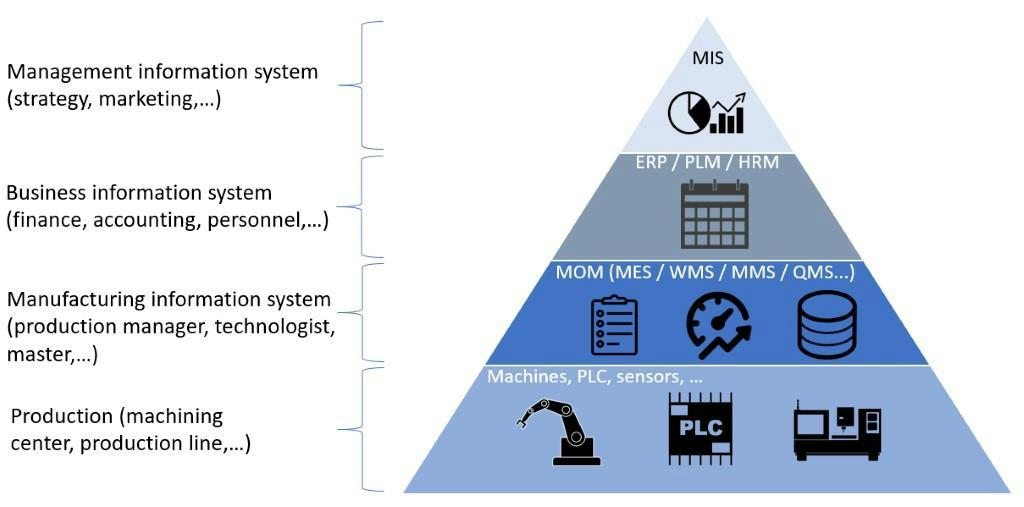
\includegraphics[width=441.64pt,height=218.2pt]{latexImage_29a65025ef358614f4e11c3d6de59c1e.png}}
\end{picture}
\newpage
\begin{tikzpicture}[overlay]\path(0pt,0pt);\end{tikzpicture}
\begin{picture}(-5,0)(2.5,0)
\put(506.14,-727.616){\fontsize{12}{1}\usefont{T1}{ptm}{m}{n}\selectfont\color{color_29791}9}
\put(512.14,-727.616){\fontsize{12}{1}\usefont{T1}{ptm}{m}{n}\selectfont\color{color_29791} }
\put(515.14,-727.616){\fontsize{12}{1}\usefont{T1}{ptm}{m}{n}\selectfont\color{color_29791} }
\put(70.104,-742.496){\fontsize{10.56}{1}\usefont{T1}{ptm}{m}{n}\selectfont\color{color_29791} }
\put(72.744,-742.496){\fontsize{12}{1}\usefont{T1}{ptm}{m}{n}\selectfont\color{color_29791} }
\put(82.944,-72.34003){\fontsize{12}{1}\usefont{T1}{ptm}{m}{n}\selectfont\color{color_29791}MES}
\put(107.652,-72.34003){\fontsize{12}{1}\usefont{T1}{ptm}{m}{n}\selectfont\color{color_29791}A}
\put(115.572,-72.34003){\fontsize{12}{1}\usefont{T1}{ptm}{m}{n}\selectfont\color{color_29791} }
\put(125.28,-72.34003){\fontsize{12}{1}\usefont{T1}{ptm}{m}{n}\selectfont\color{color_29791}I}
\put(129.12,-72.34003){\fontsize{12}{1}\usefont{T1}{ptm}{m}{n}\selectfont\color{color_29791}nter}
\put(147.72,-72.34003){\fontsize{12}{1}\usefont{T1}{ptm}{m}{n}\selectfont\color{color_29791}na}
\put(159,-72.34003){\fontsize{12}{1}\usefont{T1}{ptm}{m}{n}\selectfont\color{color_29791}ti}
\put(165.708,-72.34003){\fontsize{12}{1}\usefont{T1}{ptm}{m}{n}\selectfont\color{color_29791}ona}
\put(182.988,-72.34003){\fontsize{12}{1}\usefont{T1}{ptm}{m}{n}\selectfont\color{color_29791}l}
\put(186.41,-72.34003){\fontsize{12}{1}\usefont{T1}{ptm}{m}{n}\selectfont\color{color_29791}(}
\put(198.41,-72.34003){\fontsize{12}{1}\usefont{T1}{ptm}{m}{n}\selectfont\color{color_29791}1}
\put(204.518,-72.34003){\fontsize{12}{1}\usefont{T1}{ptm}{m}{n}\selectfont\color{color_29791}997}
\put(222.53,-72.34003){\fontsize{12}{1}\usefont{T1}{ptm}{m}{n}\selectfont\color{color_29791}年}
\put(234.53,-72.34003){\fontsize{12}{1}\usefont{T1}{ptm}{m}{n}\selectfont\color{color_29791})}
\put(246.53,-72.34003){\fontsize{12}{1}\usefont{T1}{ptm}{m}{n}\selectfont\color{color_29791}將}
\put(258.53,-72.34003){\fontsize{12}{1}\usefont{T1}{ptm}{m}{n}\selectfont\color{color_29791}MES}
\put(283.25,-72.34003){\fontsize{12}{1}\usefont{T1}{ptm}{m}{n}\selectfont\color{color_29791}的功能分為}
\put(343.27,-72.34003){\fontsize{12}{1}\usefont{T1}{ptm}{m}{n}\selectfont\color{color_29791}11}
\put(355.27,-72.34003){\fontsize{12}{1}\usefont{T1}{ptm}{m}{n}\selectfont\color{color_29791}類}
\put(367.27,-72.34003){\fontsize{12}{1}\usefont{T1}{ptm}{m}{n}\selectfont\color{color_29791};}
\put(370.63,-72.34003){\fontsize{12}{1}\usefont{T1}{ptm}{m}{n}\selectfont\color{color_29791}此外}
\put(394.63,-72.34003){\fontsize{12}{1}\usefont{T1}{ptm}{m}{n}\selectfont\color{color_29791},}
\put(406.75,-72.34003){\fontsize{12}{1}\usefont{T1}{ptm}{m}{n}\selectfont\color{color_29791}I}
\put(410.47,-72.34003){\fontsize{12}{1}\usefont{T1}{ptm}{m}{n}\selectfont\color{color_29791}S}
\put(417.178,-72.34003){\fontsize{12}{1}\usefont{T1}{ptm}{m}{n}\selectfont\color{color_29791}A95}
\put(437.926,-72.34003){\fontsize{12}{1}\usefont{T1}{ptm}{m}{n}\selectfont\color{color_29791} }
\put(447.58,-72.34003){\fontsize{12}{1}\usefont{T1}{ptm}{m}{n}\selectfont\color{color_29791}–}
\put(453.58,-72.34003){\fontsize{12}{1}\usefont{T1}{ptm}{m}{n}\selectfont\color{color_29791} }
\put(463.3,-72.34003){\fontsize{12}{1}\usefont{T1}{ptm}{m}{n}\selectfont\color{color_29791}I}
\put(467.02,-72.34003){\fontsize{12}{1}\usefont{T1}{ptm}{m}{n}\selectfont\color{color_29791}EC62264}
\put(512.488,-72.34003){\fontsize{12}{1}\usefont{T1}{ptm}{m}{n}\selectfont\color{color_29791} }
\put(69.384,-89.97998){\fontsize{12}{1}\usefont{T1}{ptm}{m}{n}\selectfont\color{color_29791}(}
\put(81.384,-89.97998){\fontsize{12}{1}\usefont{T1}{ptm}{m}{n}\selectfont\color{color_29791}2013}
\put(105.38,-89.97998){\fontsize{12}{1}\usefont{T1}{ptm}{m}{n}\selectfont\color{color_29791})}
\put(117.38,-89.97998){\fontsize{12}{1}\usefont{T1}{ptm}{m}{n}\selectfont\color{color_29791} }
\put(69.384,-107.62){\fontsize{12}{1}\usefont{T1}{ptm}{m}{n}\selectfont\color{color_29791}標準中列出了每個企業層以及每種資訊系統的任務}
\put(333.43,-107.62){\fontsize{12}{1}\usefont{T1}{ptm}{m}{n}\selectfont\color{color_29791}。}
\put(345.43,-107.62){\fontsize{12}{1}\usefont{T1}{ptm}{m}{n}\selectfont\color{color_29791}該標準還為資訊系統之間交換}
\put(69.384,-125.14){\fontsize{12}{1}\usefont{T1}{ptm}{m}{n}\selectfont\color{color_29791}的數據結構提供了定義}
\put(189.41,-125.14){\fontsize{12}{1}\usefont{T1}{ptm}{m}{n}\selectfont\color{color_29791},}
\put(201.41,-125.14){\fontsize{12}{1}\usefont{T1}{ptm}{m}{n}\selectfont\color{color_29791}旨在加強其集成}
\put(285.41,-125.14){\fontsize{12}{1}\usefont{T1}{ptm}{m}{n}\selectfont\color{color_29791};}
\put(288.77,-125.14){\fontsize{12}{1}\usefont{T1}{ptm}{m}{n}\selectfont\color{color_29791}然而}
\put(312.79,-125.14){\fontsize{12}{1}\usefont{T1}{ptm}{m}{n}\selectfont\color{color_29791},}
\put(324.79,-125.14){\fontsize{12}{1}\usefont{T1}{ptm}{m}{n}\selectfont\color{color_29791}它主要關注}
\put(384.79,-125.14){\fontsize{12}{1}\usefont{T1}{ptm}{m}{n}\selectfont\color{color_29791}ERP}
\put(406.87,-125.14){\fontsize{12}{1}\usefont{T1}{ptm}{m}{n}\selectfont\color{color_29791}-}
\put(410.83,-125.14){\fontsize{12}{1}\usefont{T1}{ptm}{m}{n}\selectfont\color{color_29791}MES}
\put(435.55,-125.14){\fontsize{12}{1}\usefont{T1}{ptm}{m}{n}\selectfont\color{color_29791}-}
\put(69.384,-142.9){\fontsize{12}{1}\usefont{T1}{ptm}{m}{n}\selectfont\color{color_29791}車間集成}
\put(117.38,-142.9){\fontsize{12}{1}\usefont{T1}{ptm}{m}{n}\selectfont\color{color_29791}(}
\put(129.38,-142.9){\fontsize{12}{1}\usefont{T1}{ptm}{m}{n}\selectfont\color{color_29791}D'A}
\put(148.82,-142.9){\fontsize{12}{1}\usefont{T1}{ptm}{m}{n}\selectfont\color{color_29791}ntoni}
\put(173.528,-142.9){\fontsize{12}{1}\usefont{T1}{ptm}{m}{n}\selectfont\color{color_29791}o e}
\put(187.808,-142.9){\fontsize{12}{1}\usefont{T1}{ptm}{m}{n}\selectfont\color{color_29791}t al.}
\put(205.85,-142.9){\fontsize{12}{1}\usefont{T1}{ptm}{m}{n}\selectfont\color{color_29791},}
\put(217.85,-142.9){\fontsize{12}{1}\usefont{T1}{ptm}{m}{n}\selectfont\color{color_29791} }
\put(220.85,-142.9){\fontsize{12}{1}\usefont{T1}{ptm}{m}{n}\selectfont\color{color_29791}2015}
\put(244.85,-142.9){\fontsize{12}{1}\usefont{T1}{ptm}{m}{n}\selectfont\color{color_29791})。}
\put(268.85,-142.9){\fontsize{12}{1}\usefont{T1}{ptm}{m}{n}\selectfont\color{color_29791} }
\put(271.85,-142.9){\fontsize{12}{1}\usefont{T1}{ptm}{m}{n}\selectfont\color{color_29791} }
\put(84.264,-160.42){\fontsize{12}{1}\usefont{T1}{ptm}{m}{n}\selectfont\color{color_29791} }
\put(87.26,-160.42){\fontsize{12}{1}\usefont{T1}{ptm}{m}{n}\selectfont\color{color_29791} }
\put(82.944,-176.38){\fontsize{12}{1}\usefont{T1}{ptm}{m}{n}\selectfont\color{color_29791}相比之下}
\put(130.94,-176.38){\fontsize{12}{1}\usefont{T1}{ptm}{m}{n}\selectfont\color{color_29791},}
\put(142.94,-176.38){\fontsize{12}{1}\usefont{T1}{ptm}{m}{n}\selectfont\color{color_29791}P}
\put(149.768,-176.38){\fontsize{12}{1}\usefont{T1}{ptm}{m}{n}\selectfont\color{color_29791}L}
\put(156.848,-176.38){\fontsize{12}{1}\usefont{T1}{ptm}{m}{n}\selectfont\color{color_29791}M}
\put(167.636,-176.38){\fontsize{12}{1}\usefont{T1}{ptm}{m}{n}\selectfont\color{color_29791} }
\put(265.37,-176.38){\fontsize{12}{1}\usefont{T1}{ptm}{m}{n}\selectfont\color{color_29791}研究要新得多}
\put(337.39,-176.38){\fontsize{12}{1}\usefont{T1}{ptm}{m}{n}\selectfont\color{color_29791},}
\put(349.39,-176.38){\fontsize{12}{1}\usefont{T1}{ptm}{m}{n}\selectfont\color{color_29791}而}
\put(361.39,-176.38){\fontsize{12}{1}\usefont{T1}{ptm}{m}{n}\selectfont\color{color_29791} }
\put(459.1,-176.38){\fontsize{12}{1}\usefont{T1}{ptm}{m}{n}\selectfont\color{color_29791}P}
\put(465.928,-176.38){\fontsize{12}{1}\usefont{T1}{ptm}{m}{n}\selectfont\color{color_29791}L}
\put(473.008,-176.38){\fontsize{12}{1}\usefont{T1}{ptm}{m}{n}\selectfont\color{color_29791}M}
\put(483.82,-176.38){\fontsize{12}{1}\usefont{T1}{ptm}{m}{n}\selectfont\color{color_29791}-}
\put(487.78,-176.38){\fontsize{12}{1}\usefont{T1}{ptm}{m}{n}\selectfont\color{color_29791}MES}
\put(512.488,-176.38){\fontsize{12}{1}\usefont{T1}{ptm}{m}{n}\selectfont\color{color_29791} }
\put(69.384,-194.02){\fontsize{12}{1}\usefont{T1}{ptm}{m}{n}\selectfont\color{color_29791}集成是這項工作的主要重點}
\put(213.41,-194.02){\fontsize{12}{1}\usefont{T1}{ptm}{m}{n}\selectfont\color{color_29791},}
\put(225.41,-194.02){\fontsize{12}{1}\usefont{T1}{ptm}{m}{n}\selectfont\color{color_29791}更是如此}
\put(273.41,-194.02){\fontsize{12}{1}\usefont{T1}{ptm}{m}{n}\selectfont\color{color_29791}。(}
\put(297.41,-194.02){\fontsize{12}{1}\usefont{T1}{ptm}{m}{n}\selectfont\color{color_29791}第}
\put(309.41,-194.02){\fontsize{12}{1}\usefont{T1}{ptm}{m}{n}\selectfont\color{color_29791}3}
\put(315.43,-194.02){\fontsize{12}{1}\usefont{T1}{ptm}{m}{n}\selectfont\color{color_29791}章}
\put(327.43,-194.02){\fontsize{12}{1}\usefont{T1}{ptm}{m}{n}\selectfont\color{color_29791})}
\put(339.43,-194.02){\fontsize{12}{1}\usefont{T1}{ptm}{m}{n}\selectfont\color{color_29791}介紹了這種整合的挑戰和最新的}
\put(69.384,-211.54){\fontsize{12}{1}\usefont{T1}{ptm}{m}{n}\selectfont\color{color_29791}技術}
\put(93.38,-211.54){\fontsize{12}{1}\usefont{T1}{ptm}{m}{n}\selectfont\color{color_29791},}
\put(105.38,-211.54){\fontsize{12}{1}\usefont{T1}{ptm}{m}{n}\selectfont\color{color_29791}以及它背後的理論結構}
\put(225.41,-211.54){\fontsize{12}{1}\usefont{T1}{ptm}{m}{n}\selectfont\color{color_29791}。}
\put(237.41,-211.54){\fontsize{12}{1}\usefont{T1}{ptm}{m}{n}\selectfont\color{color_29791}現在}
\put(261.41,-211.54){\fontsize{12}{1}\usefont{T1}{ptm}{m}{n}\selectfont\color{color_29791},}
\put(273.41,-211.54){\fontsize{12}{1}\usefont{T1}{ptm}{m}{n}\selectfont\color{color_29791}我只想指出}
\put(333.43,-211.54){\fontsize{12}{1}\usefont{T1}{ptm}{m}{n}\selectfont\color{color_29791},}
\put(345.43,-211.54){\fontsize{12}{1}\usefont{T1}{ptm}{m}{n}\selectfont\color{color_29791}由於}
\put(369.43,-211.54){\fontsize{12}{1}\usefont{T1}{ptm}{m}{n}\selectfont\color{color_29791}MES}
\put(394.15,-211.54){\fontsize{12}{1}\usefont{T1}{ptm}{m}{n}\selectfont\color{color_29791}提供反饋}
\put(442.15,-211.54){\fontsize{12}{1}\usefont{T1}{ptm}{m}{n}\selectfont\color{color_29791},}
\put(454.18,-211.54){\fontsize{12}{1}\usefont{T1}{ptm}{m}{n}\selectfont\color{color_29791}通過以檔}
\put(69.384,-229.18){\fontsize{12}{1}\usefont{T1}{ptm}{m}{n}\selectfont\color{color_29791}的形式生成資訊來協調更改並驗證結果}
\put(273.41,-229.18){\fontsize{12}{1}\usefont{T1}{ptm}{m}{n}\selectfont\color{color_29791},}
\put(285.41,-229.18){\fontsize{12}{1}\usefont{T1}{ptm}{m}{n}\selectfont\color{color_29791}而}
\put(297.41,-229.18){\fontsize{12}{1}\usefont{T1}{ptm}{m}{n}\selectfont\color{color_29791}P}
\put(304.238,-229.18){\fontsize{12}{1}\usefont{T1}{ptm}{m}{n}\selectfont\color{color_29791}L}
\put(311.438,-229.18){\fontsize{12}{1}\usefont{T1}{ptm}{m}{n}\selectfont\color{color_29791}M}
\put(322.15,-229.18){\fontsize{12}{1}\usefont{T1}{ptm}{m}{n}\selectfont\color{color_29791}則專注於按檔組織跟蹤更改}
\put(466.18,-229.18){\fontsize{12}{1}\usefont{T1}{ptm}{m}{n}\selectfont\color{color_29791},}
\put(478.18,-229.18){\fontsize{12}{1}\usefont{T1}{ptm}{m}{n}\selectfont\color{color_29791}因此}
\put(502.18,-229.18){\fontsize{12}{1}\usefont{T1}{ptm}{m}{n}\selectfont\color{color_29791}P}
\put(69.384,-246.97){\fontsize{12}{1}\usefont{T1}{ptm}{m}{n}\selectfont\color{color_29791}LM}
\put(87.26,-246.97){\fontsize{12}{1}\usefont{T1}{ptm}{m}{n}\selectfont\color{color_29791}-}
\put(91.22,-246.97){\fontsize{12}{1}\usefont{T1}{ptm}{m}{n}\selectfont\color{color_29791}MES}
\put(115.94,-246.97){\fontsize{12}{1}\usefont{T1}{ptm}{m}{n}\selectfont\color{color_29791}集成肯定具有}
\put(188.048,-246.97){\fontsize{12}{1}\usefont{T1}{ptm}{m}{n}\selectfont\color{color_29791}價值}
\put(212.09,-246.97){\fontsize{12}{1}\usefont{T1}{ptm}{m}{n}\selectfont\color{color_29791}。}
\put(224.09,-246.97){\fontsize{12}{1}\usefont{T1}{ptm}{m}{n}\selectfont\color{color_29791} }
\put(227.09,-246.97){\fontsize{12}{1}\usefont{T1}{ptm}{m}{n}\selectfont\color{color_29791} }
\put(70.104,-264.49){\fontsize{11.04}{1}\usefont{T1}{uarial}{m}{n}\selectfont\color{color_275101} }
\put(73.104,-264.49){\fontsize{12}{1}\usefont{T1}{ptm}{m}{n}\selectfont\color{color_29791} }
\put(87.38,-297.25){\fontsize{14.04}{1}\usefont{T1}{ptm}{b}{n}\selectfont\color{color_29791}2}
\put(94.44212,-297.25){\fontsize{14.04}{1}\usefont{T1}{ptm}{b}{n}\selectfont\color{color_29791}.4. }
\put(111.86,-297.25){\fontsize{14.04}{1}\usefont{T1}{ptm}{m}{n}\selectfont\color{color_29791}工業}
\put(139.94,-297.25){\fontsize{14.04}{1}\usefont{T1}{ptm}{b}{n}\selectfont\color{color_29791}4}
\put(147.0021,-297.25){\fontsize{14.04}{1}\usefont{T1}{ptm}{b}{n}\selectfont\color{color_29791}.0  }
\put(164.42,-297.25){\fontsize{14.04}{1}\usefont{T1}{ptm}{b}{n}\selectfont\color{color_29791} }
\put(82.944,-331.69){\fontsize{12}{1}\usefont{T1}{ptm}{m}{n}\selectfont\color{color_29791}工業}
\put(106.94,-331.69){\fontsize{12}{1}\usefont{T1}{ptm}{m}{n}\selectfont\color{color_29791} }
\put(497.5,-331.69){\fontsize{12}{1}\usefont{T1}{ptm}{m}{n}\selectfont\color{color_29791}4.0 }
\put(69.384,-349.33){\fontsize{12}{1}\usefont{T1}{ptm}{m}{n}\selectfont\color{color_29791}一詞在現代文獻中一再被提及}
\put(225.41,-349.33){\fontsize{12}{1}\usefont{T1}{ptm}{m}{n}\selectfont\color{color_29791},}
\put(237.41,-349.33){\fontsize{12}{1}\usefont{T1}{ptm}{m}{n}\selectfont\color{color_29791}作為生產發展的下一步或當前步驟}
\put(417.43,-349.33){\fontsize{12}{1}\usefont{T1}{ptm}{m}{n}\selectfont\color{color_29791}。}
\put(429.43,-349.33){\fontsize{12}{1}\usefont{T1}{ptm}{m}{n}\selectfont\color{color_29791}它代表了第四}
\put(69.384,-366.97){\fontsize{12}{1}\usefont{T1}{ptm}{m}{n}\selectfont\color{color_29791}次工業革命}
\put(129.38,-366.97){\fontsize{12}{1}\usefont{T1}{ptm}{m}{n}\selectfont\color{color_29791},}
\put(141.38,-366.97){\fontsize{12}{1}\usefont{T1}{ptm}{m}{n}\selectfont\color{color_29791}第一次工業革命以採用蒸汽動力為標誌}
\put(345.43,-366.97){\fontsize{12}{1}\usefont{T1}{ptm}{m}{n}\selectfont\color{color_29791},}
\put(357.43,-366.97){\fontsize{12}{1}\usefont{T1}{ptm}{m}{n}\selectfont\color{color_29791}第二次以主要使用電力為標}
\put(69.384,-384.73){\fontsize{12}{1}\usefont{T1}{ptm}{m}{n}\selectfont\color{color_29791}誌}
\put(81.384,-384.73){\fontsize{12}{1}\usefont{T1}{ptm}{m}{n}\selectfont\color{color_29791},}
\put(93.38,-384.73){\fontsize{12}{1}\usefont{T1}{ptm}{m}{n}\selectfont\color{color_29791}第三次以數位技術的實施為特徵}
\put(261.41,-384.73){\fontsize{12}{1}\usefont{T1}{ptm}{m}{n}\selectfont\color{color_29791}。}
\put(273.41,-384.73){\fontsize{12}{1}\usefont{T1}{ptm}{m}{n}\selectfont\color{color_29791}圖}
\put(285.41,-384.73){\fontsize{12}{1}\usefont{T1}{ptm}{m}{n}\selectfont\color{color_29791}5}
\put(291.41,-384.73){\fontsize{12}{1}\usefont{T1}{ptm}{m}{n}\selectfont\color{color_29791}很好地代表了工業革命的進展}
\put(447.46,-384.73){\fontsize{12}{1}\usefont{T1}{ptm}{m}{n}\selectfont\color{color_29791}。}
\put(459.46,-384.73){\fontsize{12}{1}\usefont{T1}{ptm}{m}{n}\selectfont\color{color_29791} }
\put(462.46,-384.73){\fontsize{12}{1}\usefont{T1}{ptm}{m}{n}\selectfont\color{color_29791} }
\put(507.46,-623.7){\fontsize{12}{1}\usefont{T1}{ptm}{m}{n}\selectfont\color{color_29791} }
\put(510.46,-623.7){\fontsize{12}{1}\usefont{T1}{ptm}{m}{n}\selectfont\color{color_29791} }
\put(164.18,-636.06){\fontsize{12}{1}\usefont{T1}{ptm}{m}{n}\selectfont\color{color_29791}圖}
\put(176.3,-636.06){\fontsize{12}{1}\usefont{T1}{ptm}{b}{n}\selectfont\color{color_29791}5}
\put(182.21,-636.06){\fontsize{12}{1}\usefont{T1}{ptm}{m}{n}\selectfont\color{color_29791}行業演}
\put(218.318,-636.06){\fontsize{12}{1}\usefont{T1}{ptm}{m}{n}\selectfont\color{color_29791}變}
\put(230.33,-636.06){\fontsize{12}{1}\usefont{T1}{ptm}{m}{n}\selectfont\color{color_29791}(}
\put(242.33,-636.06){\fontsize{12}{1}\usefont{T1}{ptm}{m}{n}\selectfont\color{color_29791}改編自}
\put(278.45,-636.06){\fontsize{12}{1}\usefont{T1}{ptm}{b}{n}\selectfont\color{color_29791}S}
\put(285.05,-636.06){\fontsize{12}{1}\usefont{T1}{ptm}{b}{n}\selectfont\color{color_29791}T}
\put(292.25,-636.06){\fontsize{12}{1}\usefont{T1}{ptm}{b}{n}\selectfont\color{color_29791}AN}
\put(309.53,-636.06){\fontsize{12}{1}\usefont{T1}{ptm}{b}{n}\selectfont\color{color_29791}CIOIU }
\put(347.81,-636.06){\fontsize{12}{1}\usefont{T1}{ptm}{b}{n}\selectfont\color{color_29791}Alin}
\put(369.91,-636.06){\fontsize{12}{1}\usefont{T1}{ptm}{m}{n}\selectfont\color{color_29791},}
\put(382.03,-636.06){\fontsize{12}{1}\usefont{T1}{ptm}{b}{n}\selectfont\color{color_29791}2017}
\put(405.91,-636.06){\fontsize{12}{1}\usefont{T1}{ptm}{m}{n}\selectfont\color{color_29791})}
\put(418.03,-636.06){\fontsize{12}{1}\usefont{T1}{ptm}{b}{n}\selectfont\color{color_29791} }
\put(420.91,-636.06){\fontsize{12}{1}\usefont{T1}{ptm}{m}{n}\selectfont\color{color_29791} }
\put(84.264,-653.46){\fontsize{12}{1}\usefont{T1}{ptm}{m}{n}\selectfont\color{color_29791} }
\put(87.26,-653.46){\fontsize{12}{1}\usefont{T1}{ptm}{m}{n}\selectfont\color{color_29791} }
\put(82.944,-669.42){\fontsize{12}{1}\usefont{T1}{ptm}{m}{n}\selectfont\color{color_29791}從廣義上講}
\put(142.94,-669.42){\fontsize{12}{1}\usefont{T1}{ptm}{m}{n}\selectfont\color{color_29791},}
\put(154.94,-669.42){\fontsize{12}{1}\usefont{T1}{ptm}{m}{n}\selectfont\color{color_29791}第四次工業革命最終以數位連接與生產之間的全面融合為標誌}
\put(479.02,-669.42){\fontsize{12}{1}\usefont{T1}{ptm}{m}{n}\selectfont\color{color_29791}。}
\put(491.02,-669.42){\fontsize{12}{1}\usefont{T1}{ptm}{m}{n}\selectfont\color{color_29791}眾}
\put(69.384,-687.056){\fontsize{12}{1}\usefont{T1}{ptm}{m}{n}\selectfont\color{color_29791}所周知}
\put(105.38,-687.056){\fontsize{12}{1}\usefont{T1}{ptm}{m}{n}\selectfont\color{color_29791},}
\put(117.38,-687.056){\fontsize{12}{1}\usefont{T1}{ptm}{m}{n}\selectfont\color{color_29791}數位網路的發展是維持現代世界的關鍵技術}
\put(345.43,-687.056){\fontsize{12}{1}\usefont{T1}{ptm}{m}{n}\selectfont\color{color_29791}。}
\put(357.43,-687.056){\fontsize{12}{1}\usefont{T1}{ptm}{m}{n}\selectfont\color{color_29791}它改變了人類互動和做生意}
\put(69.384,-704.576){\fontsize{12}{1}\usefont{T1}{ptm}{m}{n}\selectfont\color{color_29791}的方式}
\put(105.38,-704.576){\fontsize{12}{1}\usefont{T1}{ptm}{m}{n}\selectfont\color{color_29791}。}
\put(117.38,-704.576){\fontsize{12}{1}\usefont{T1}{ptm}{m}{n}\selectfont\color{color_29791}然而}
\put(141.38,-704.576){\fontsize{12}{1}\usefont{T1}{ptm}{m}{n}\selectfont\color{color_29791},}
\put(153.38,-704.576){\fontsize{12}{1}\usefont{T1}{ptm}{m}{n}\selectfont\color{color_29791}目前應用於工業的水準是否構成工業革命仍然不確定}
\put(429.43,-704.576){\fontsize{12}{1}\usefont{T1}{ptm}{m}{n}\selectfont\color{color_29791},}
\put(441.43,-704.576){\fontsize{12}{1}\usefont{T1}{ptm}{m}{n}\selectfont\color{color_29791}因為在所有}
\put(73.1,-623.5){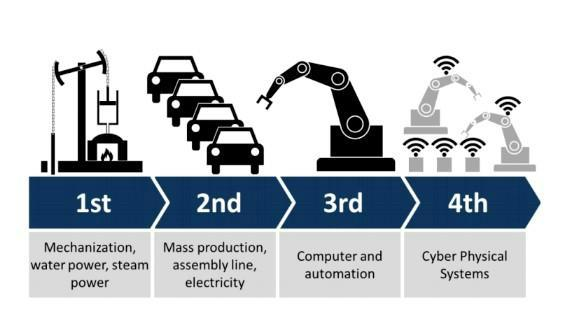
\includegraphics[width=434.25pt,height=232.5pt]{latexImage_f409e6a889646f22c3e3fe505a15dc47.png}}
\end{picture}
\newpage
\begin{tikzpicture}[overlay]\path(0pt,0pt);\end{tikzpicture}
\begin{picture}(-5,0)(2.5,0)
\put(500.14,-727.616){\fontsize{12}{1}\usefont{T1}{ptm}{m}{n}\selectfont\color{color_29791}10}
\put(512.14,-727.616){\fontsize{12}{1}\usefont{T1}{ptm}{m}{n}\selectfont\color{color_29791} }
\put(515.14,-727.616){\fontsize{12}{1}\usefont{T1}{ptm}{m}{n}\selectfont\color{color_29791} }
\put(70.104,-742.496){\fontsize{10.56}{1}\usefont{T1}{ptm}{m}{n}\selectfont\color{color_29791} }
\put(72.744,-742.496){\fontsize{12}{1}\usefont{T1}{ptm}{m}{n}\selectfont\color{color_29791} }
\put(69.384,-72.34003){\fontsize{12}{1}\usefont{T1}{ptm}{m}{n}\selectfont\color{color_29791}其他革命中}
\put(129.38,-72.34003){\fontsize{12}{1}\usefont{T1}{ptm}{m}{n}\selectfont\color{color_29791},}
\put(141.38,-72.34003){\fontsize{12}{1}\usefont{T1}{ptm}{m}{n}\selectfont\color{color_29791}都以產量的急劇增加為標誌}
\put(285.41,-72.34003){\fontsize{12}{1}\usefont{T1}{ptm}{m}{n}\selectfont\color{color_29791},}
\put(297.41,-72.34003){\fontsize{12}{1}\usefont{T1}{ptm}{m}{n}\selectfont\color{color_29791}而這一次尚未發生}
\put(393.43,-72.34003){\fontsize{12}{1}\usefont{T1}{ptm}{m}{n}\selectfont\color{color_29791}。}
\put(405.43,-72.34003){\fontsize{12}{1}\usefont{T1}{ptm}{m}{n}\selectfont\color{color_29791}事實上}
\put(441.43,-72.34003){\fontsize{12}{1}\usefont{T1}{ptm}{m}{n}\selectfont\color{color_29791},}
\put(453.46,-72.34003){\fontsize{12}{1}\usefont{T1}{ptm}{m}{n}\selectfont\color{color_29791}我們仍有}
\put(69.384,-90.09998){\fontsize{12}{1}\usefont{T1}{ptm}{m}{n}\selectfont\color{color_29791}待達成工業}
\put(129.38,-90.09998){\fontsize{12}{1}\usefont{T1}{ptm}{m}{n}\selectfont\color{color_29791}4.0}
\put(144.38,-90.09998){\fontsize{12}{1}\usefont{T1}{ptm}{m}{n}\selectfont\color{color_29791}的共同定義}
\put(204.41,-90.09998){\fontsize{12}{1}\usefont{T1}{ptm}{m}{n}\selectfont\color{color_29791}。}
\put(216.41,-90.09998){\fontsize{12}{1}\usefont{T1}{ptm}{m}{n}\selectfont\color{color_29791} }
\put(219.41,-90.09998){\fontsize{12}{1}\usefont{T1}{ptm}{m}{n}\selectfont\color{color_29791} }
\put(84.264,-107.5){\fontsize{12}{1}\usefont{T1}{ptm}{m}{n}\selectfont\color{color_29791} }
\put(87.26,-107.5){\fontsize{12}{1}\usefont{T1}{ptm}{m}{n}\selectfont\color{color_29791} }
\put(82.944,-123.46){\fontsize{12}{1}\usefont{T1}{ptm}{m}{n}\selectfont\color{color_29791}然而}
\put(106.94,-123.46){\fontsize{12}{1}\usefont{T1}{ptm}{m}{n}\selectfont\color{color_29791},}
\put(118.94,-123.46){\fontsize{12}{1}\usefont{T1}{ptm}{m}{n}\selectfont\color{color_29791}被廣泛接受的是}
\put(202.97,-123.46){\fontsize{12}{1}\usefont{T1}{ptm}{m}{n}\selectfont\color{color_29791},}
\put(214.97,-123.46){\fontsize{12}{1}\usefont{T1}{ptm}{m}{n}\selectfont\color{color_29791}至少有}
\put(250.97,-123.46){\fontsize{12}{1}\usefont{T1}{ptm}{m}{n}\selectfont\color{color_29791} }
\put(263.09,-123.46){\fontsize{12}{1}\usefont{T1}{ptm}{m}{n}\selectfont\color{color_29791}3 }
\put(281.21,-123.46){\fontsize{12}{1}\usefont{T1}{ptm}{m}{n}\selectfont\color{color_29791}種技術是工業}
\put(353.23,-123.46){\fontsize{12}{1}\usefont{T1}{ptm}{m}{n}\selectfont\color{color_29791} }
\put(365.35,-123.46){\fontsize{12}{1}\usefont{T1}{ptm}{m}{n}\selectfont\color{color_29791}4.0 }
\put(392.47,-123.46){\fontsize{12}{1}\usefont{T1}{ptm}{m}{n}\selectfont\color{color_29791}的特徵}
\put(428.47,-123.46){\fontsize{12}{1}\usefont{T1}{ptm}{m}{n}\selectfont\color{color_29791}。}
\put(440.47,-123.46){\fontsize{12}{1}\usefont{T1}{ptm}{m}{n}\selectfont\color{color_29791}這些是物聯網}
\put(512.5,-123.46){\fontsize{12}{1}\usefont{T1}{ptm}{m}{n}\selectfont\color{color_29791} }
\put(69.384,-141.1){\fontsize{12}{1}\usefont{T1}{ptm}{m}{n}\selectfont\color{color_29791}(}
\put(81.504,-141.1){\fontsize{12}{1}\usefont{T1}{ptm}{m}{n}\selectfont\color{color_29791}I}
\put(85.224,-141.1){\fontsize{12}{1}\usefont{T1}{ptm}{m}{n}\selectfont\color{color_29791}oT}
\put(98.54,-141.1){\fontsize{12}{1}\usefont{T1}{ptm}{m}{n}\selectfont\color{color_29791})、}
\put(122.54,-141.1){\fontsize{12}{1}\usefont{T1}{ptm}{m}{n}\selectfont\color{color_29791}雲計算和資}
\put(182.648,-141.1){\fontsize{12}{1}\usefont{T1}{ptm}{m}{n}\selectfont\color{color_29791}訊物理系統}
\put(242.69,-141.1){\fontsize{12}{1}\usefont{T1}{ptm}{m}{n}\selectfont\color{color_29791} }
\put(467.14,-141.1){\fontsize{12}{1}\usefont{T1}{ptm}{m}{n}\selectfont\color{color_29791}(}
\put(479.14,-141.1){\fontsize{12}{1}\usefont{T1}{ptm}{m}{n}\selectfont\color{color_29791}C}
\put(487.168,-141.1){\fontsize{12}{1}\usefont{T1}{ptm}{m}{n}\selectfont\color{color_29791}P}
\put(493.876,-141.1){\fontsize{12}{1}\usefont{T1}{ptm}{m}{n}\selectfont\color{color_29791}S}
\put(500.62,-141.1){\fontsize{12}{1}\usefont{T1}{ptm}{m}{n}\selectfont\color{color_29791})}
\put(512.5,-141.1){\fontsize{12}{1}\usefont{T1}{ptm}{m}{n}\selectfont\color{color_29791} }
\put(69.384,-158.86){\fontsize{12}{1}\usefont{T1}{ptm}{m}{n}\selectfont\color{color_29791}的發展}
\put(105.38,-158.86){\fontsize{12}{1}\usefont{T1}{ptm}{m}{n}\selectfont\color{color_29791},}
\put(117.38,-158.86){\fontsize{12}{1}\usefont{T1}{ptm}{m}{n}\selectfont\color{color_29791}其中最後一個對於本論文的背景尤為重要}
\put(333.43,-158.86){\fontsize{12}{1}\usefont{T1}{ptm}{m}{n}\selectfont\color{color_29791}。}
\put(345.43,-158.86){\fontsize{12}{1}\usefont{T1}{ptm}{m}{n}\selectfont\color{color_29791}  }
\put(351.43,-158.86){\fontsize{12}{1}\usefont{T1}{ptm}{m}{n}\selectfont\color{color_29791} }
\put(84.264,-176.26){\fontsize{12}{1}\usefont{T1}{ptm}{m}{n}\selectfont\color{color_29791} }
\put(87.26,-176.26){\fontsize{12}{1}\usefont{T1}{ptm}{m}{n}\selectfont\color{color_29791} }
\put(82.944,-192.22){\fontsize{12}{1}\usefont{T1}{ptm}{m}{n}\selectfont\color{color_29791}C}
\put(90.972,-192.22){\fontsize{12}{1}\usefont{T1}{ptm}{m}{n}\selectfont\color{color_29791}P}
\put(97.68,-192.22){\fontsize{12}{1}\usefont{T1}{ptm}{m}{n}\selectfont\color{color_29791}S}
\put(104.42,-192.22){\fontsize{12}{1}\usefont{T1}{ptm}{m}{n}\selectfont\color{color_29791}是由一個真實實體}
\put(200.33,-192.22){\fontsize{12}{1}\usefont{T1}{ptm}{m}{n}\selectfont\color{color_29791}(}
\put(212.33,-192.22){\fontsize{12}{1}\usefont{T1}{ptm}{m}{n}\selectfont\color{color_29791}例如}
\put(236.33,-192.22){\fontsize{12}{1}\usefont{T1}{ptm}{m}{n}\selectfont\color{color_29791},}
\put(248.33,-192.22){\fontsize{12}{1}\usefont{T1}{ptm}{m}{n}\selectfont\color{color_29791}一台機器}
\put(296.33,-192.22){\fontsize{12}{1}\usefont{T1}{ptm}{m}{n}\selectfont\color{color_29791})}
\put(308.33,-192.22){\fontsize{12}{1}\usefont{T1}{ptm}{m}{n}\selectfont\color{color_29791}及其相應的虛擬模型組成的系統}
\put(476.38,-192.22){\fontsize{12}{1}\usefont{T1}{ptm}{m}{n}\selectfont\color{color_29791}——}
\put(69.384,-209.86){\fontsize{12}{1}\usefont{T1}{ptm}{m}{n}\selectfont\color{color_29791}嵌入所有模型以模仿真實對應物的行為}
\put(273.41,-209.86){\fontsize{12}{1}\usefont{T1}{ptm}{m}{n}\selectfont\color{color_29791}——}
\put(69.384,-227.5){\fontsize{12}{1}\usefont{T1}{ptm}{m}{n}\selectfont\color{color_29791}能夠相互通信}
\put(141.38,-227.5){\fontsize{12}{1}\usefont{T1}{ptm}{m}{n}\selectfont\color{color_29791}(}
\put(153.38,-227.5){\fontsize{12}{1}\usefont{T1}{ptm}{m}{n}\selectfont\color{color_29791}D}
\put(162.02,-227.5){\fontsize{12}{1}\usefont{T1}{ptm}{m}{n}\selectfont\color{color_29791}』}
\put(174.02,-227.5){\fontsize{12}{1}\usefont{T1}{ptm}{m}{n}\selectfont\color{color_29791}Antonio}
\put(213.41,-227.5){\fontsize{12}{1}\usefont{T1}{ptm}{m}{n}\selectfont\color{color_29791}等人}
\put(237.41,-227.5){\fontsize{12}{1}\usefont{T1}{ptm}{m}{n}\selectfont\color{color_29791},}
\put(249.41,-227.5){\fontsize{12}{1}\usefont{T1}{ptm}{m}{n}\selectfont\color{color_29791}2017}
\put(273.41,-227.5){\fontsize{12}{1}\usefont{T1}{ptm}{m}{n}\selectfont\color{color_29791})。}
\put(297.41,-227.5){\fontsize{12}{1}\usefont{T1}{ptm}{m}{n}\selectfont\color{color_29791}這個想法是}
\put(357.43,-227.5){\fontsize{12}{1}\usefont{T1}{ptm}{m}{n}\selectfont\color{color_29791},}
\put(369.43,-227.5){\fontsize{12}{1}\usefont{T1}{ptm}{m}{n}\selectfont\color{color_29791}如果一個人要開發一個關}
\put(69.384,-245.17){\fontsize{12}{1}\usefont{T1}{ptm}{m}{n}\selectfont\color{color_29791}於系統中過程的所有物理儀器的數位孿生}
\put(285.41,-245.17){\fontsize{12}{1}\usefont{T1}{ptm}{m}{n}\selectfont\color{color_29791} }
\put(69.384,-262.81){\fontsize{12}{1}\usefont{T1}{ptm}{m}{n}\selectfont\color{color_29791}(}
\put(81.384,-262.81){\fontsize{12}{1}\usefont{T1}{ptm}{m}{n}\selectfont\color{color_29791}DT}
\put(97.34,-262.81){\fontsize{12}{1}\usefont{T1}{ptm}{m}{n}\selectfont\color{color_29791}),}
\put(121.34,-262.81){\fontsize{12}{1}\usefont{T1}{ptm}{m}{n}\selectfont\color{color_29791}該過程允許數字對應物相互交互以及與物理世界交互}
\put(397.39,-262.81){\fontsize{12}{1}\usefont{T1}{ptm}{m}{n}\selectfont\color{color_29791},}
\put(409.39,-262.81){\fontsize{12}{1}\usefont{T1}{ptm}{m}{n}\selectfont\color{color_29791}那麼所述過程的創}
\put(69.384,-280.33){\fontsize{12}{1}\usefont{T1}{ptm}{m}{n}\selectfont\color{color_29791}新或變化將更快}
\put(153.38,-280.33){\fontsize{12}{1}\usefont{T1}{ptm}{m}{n}\selectfont\color{color_29791}、}
\put(165.38,-280.33){\fontsize{12}{1}\usefont{T1}{ptm}{m}{n}\selectfont\color{color_29791}更有效地發生}
\put(237.41,-280.33){\fontsize{12}{1}\usefont{T1}{ptm}{m}{n}\selectfont\color{color_29791}。}
\put(249.41,-280.33){\fontsize{12}{1}\usefont{T1}{ptm}{m}{n}\selectfont\color{color_29791}例如}
\put(273.41,-280.33){\fontsize{12}{1}\usefont{T1}{ptm}{m}{n}\selectfont\color{color_29791},}
\put(285.41,-280.33){\fontsize{12}{1}\usefont{T1}{ptm}{m}{n}\selectfont\color{color_29791}工程師可以使用}
\put(369.43,-280.33){\fontsize{12}{1}\usefont{T1}{ptm}{m}{n}\selectfont\color{color_29791}DT}
\put(385.39,-280.33){\fontsize{12}{1}\usefont{T1}{ptm}{m}{n}\selectfont\color{color_29791}的交互來類比變化}
\put(481.42,-280.33){\fontsize{12}{1}\usefont{T1}{ptm}{m}{n}\selectfont\color{color_29791},}
\put(493.42,-280.33){\fontsize{12}{1}\usefont{T1}{ptm}{m}{n}\selectfont\color{color_29791}然}
\put(69.384,-297.97){\fontsize{12}{1}\usefont{T1}{ptm}{m}{n}\selectfont\color{color_29791}後}
\put(81.384,-297.97){\fontsize{12}{1}\usefont{T1}{ptm}{m}{n}\selectfont\color{color_29791},}
\put(93.38,-297.97){\fontsize{12}{1}\usefont{T1}{ptm}{m}{n}\selectfont\color{color_29791}如果成功}
\put(141.38,-297.97){\fontsize{12}{1}\usefont{T1}{ptm}{m}{n}\selectfont\color{color_29791},}
\put(153.38,-297.97){\fontsize{12}{1}\usefont{T1}{ptm}{m}{n}\selectfont\color{color_29791}可以即時將變化自動應用於生產線}
\put(333.43,-297.97){\fontsize{12}{1}\usefont{T1}{ptm}{m}{n}\selectfont\color{color_29791},}
\put(345.43,-297.97){\fontsize{12}{1}\usefont{T1}{ptm}{m}{n}\selectfont\color{color_29791}執行測試}
\put(393.43,-297.97){\fontsize{12}{1}\usefont{T1}{ptm}{m}{n}\selectfont\color{color_29791},}
\put(405.43,-297.97){\fontsize{12}{1}\usefont{T1}{ptm}{m}{n}\selectfont\color{color_29791}收集數據並將其反}
\put(69.384,-315.73){\fontsize{12}{1}\usefont{T1}{ptm}{m}{n}\selectfont\color{color_29791}饋}
\put(81.384,-315.73){\fontsize{12}{1}\usefont{T1}{ptm}{m}{n}\selectfont\color{color_29791}給系統}
\put(117.38,-315.73){\fontsize{12}{1}\usefont{T1}{ptm}{m}{n}\selectfont\color{color_29791},}
\put(129.38,-315.73){\fontsize{12}{1}\usefont{T1}{ptm}{m}{n}\selectfont\color{color_29791}而無需手動輸入}
\put(213.41,-315.73){\fontsize{12}{1}\usefont{T1}{ptm}{m}{n}\selectfont\color{color_29791},}
\put(225.41,-315.73){\fontsize{12}{1}\usefont{T1}{ptm}{m}{n}\selectfont\color{color_29791}所有這些都通過網路完成}
\put(357.43,-315.73){\fontsize{12}{1}\usefont{T1}{ptm}{m}{n}\selectfont\color{color_29791}。}
\put(369.43,-315.73){\fontsize{12}{1}\usefont{T1}{ptm}{m}{n}\selectfont\color{color_29791} }
\put(372.43,-315.73){\fontsize{12}{1}\usefont{T1}{ptm}{m}{n}\selectfont\color{color_29791} }
\put(84.264,-333.25){\fontsize{12}{1}\usefont{T1}{ptm}{m}{n}\selectfont\color{color_29791} }
\put(87.26,-333.25){\fontsize{12}{1}\usefont{T1}{ptm}{m}{n}\selectfont\color{color_29791} }
\put(82.944,-349.21){\fontsize{12}{1}\usefont{T1}{ptm}{m}{n}\selectfont\color{color_29791}從這一切中得出的要點是}
\put(214.97,-349.21){\fontsize{12}{1}\usefont{T1}{ptm}{m}{n}\selectfont\color{color_29791},}
\put(226.97,-349.21){\fontsize{12}{1}\usefont{T1}{ptm}{m}{n}\selectfont\color{color_29791}P}
\put(233.798,-349.21){\fontsize{12}{1}\usefont{T1}{ptm}{m}{n}\selectfont\color{color_29791}L}
\put(240.878,-349.21){\fontsize{12}{1}\usefont{T1}{ptm}{m}{n}\selectfont\color{color_29791}M}
\put(251.57,-349.21){\fontsize{12}{1}\usefont{T1}{ptm}{m}{n}\selectfont\color{color_29791}-}
\put(69.384,-366.73){\fontsize{12}{1}\usefont{T1}{ptm}{m}{n}\selectfont\color{color_29791}MES}
\put(94.1,-366.73){\fontsize{12}{1}\usefont{T1}{ptm}{m}{n}\selectfont\color{color_29791}系統可能是實現適當}
\put(202.13,-366.73){\fontsize{12}{1}\usefont{T1}{ptm}{m}{n}\selectfont\color{color_29791}C}
\put(210.158,-366.73){\fontsize{12}{1}\usefont{T1}{ptm}{m}{n}\selectfont\color{color_29791}P}
\put(216.866,-366.73){\fontsize{12}{1}\usefont{T1}{ptm}{m}{n}\selectfont\color{color_29791}S}
\put(223.61,-366.73){\fontsize{12}{1}\usefont{T1}{ptm}{m}{n}\selectfont\color{color_29791}的第一步}
\put(271.61,-366.73){\fontsize{12}{1}\usefont{T1}{ptm}{m}{n}\selectfont\color{color_29791},}
\put(283.61,-366.73){\fontsize{12}{1}\usefont{T1}{ptm}{m}{n}\selectfont\color{color_29791}因為}
\put(307.49,-366.73){\fontsize{12}{1}\usefont{T1}{ptm}{m}{n}\selectfont\color{color_29791}它提供了虛擬化和必要的控制}
\put(463.54,-366.73){\fontsize{12}{1}\usefont{T1}{ptm}{m}{n}\selectfont\color{color_29791},}
\put(475.54,-366.73){\fontsize{12}{1}\usefont{T1}{ptm}{m}{n}\selectfont\color{color_29791}以達到}
\put(69.384,-384.49){\fontsize{12}{1}\usefont{T1}{ptm}{m}{n}\selectfont\color{color_29791}虛擬孿生體附近的東西}
\put(189.41,-384.49){\fontsize{12}{1}\usefont{T1}{ptm}{m}{n}\selectfont\color{color_29791}。}
\put(201.41,-384.49){\fontsize{12}{1}\usefont{T1}{ptm}{m}{n}\selectfont\color{color_29791}值得商榷的是}
\put(273.41,-384.49){\fontsize{12}{1}\usefont{T1}{ptm}{m}{n}\selectfont\color{color_29791},}
\put(285.41,-384.49){\fontsize{12}{1}\usefont{T1}{ptm}{m}{n}\selectfont\color{color_29791}它目前在工業應用中的影響有多深}
\put(465.46,-384.49){\fontsize{12}{1}\usefont{T1}{ptm}{m}{n}\selectfont\color{color_29791}。}
\put(477.46,-384.49){\fontsize{12}{1}\usefont{T1}{ptm}{m}{n}\selectfont\color{color_29791}  }
\put(483.46,-384.49){\fontsize{12}{1}\usefont{T1}{ptm}{m}{n}\selectfont\color{color_29791} }
\put(84.264,-402.01){\fontsize{12}{1}\usefont{T1}{ptm}{m}{n}\selectfont\color{color_29791} }
\put(87.26,-402.01){\fontsize{12}{1}\usefont{T1}{ptm}{m}{n}\selectfont\color{color_29791} }
\put(82.944,-417.99){\fontsize{12}{1}\usefont{T1}{ptm}{m}{n}\selectfont\color{color_29791}儘管如此}
\put(130.94,-417.99){\fontsize{12}{1}\usefont{T1}{ptm}{m}{n}\selectfont\color{color_29791},}
\put(142.94,-417.99){\fontsize{12}{1}\usefont{T1}{ptm}{m}{n}\selectfont\color{color_29791}工業}
\put(166.94,-417.99){\fontsize{12}{1}\usefont{T1}{ptm}{m}{n}\selectfont\color{color_29791} }
\put(497.5,-417.99){\fontsize{12}{1}\usefont{T1}{ptm}{m}{n}\selectfont\color{color_29791}4.0 }
\put(69.384,-435.51){\fontsize{12}{1}\usefont{T1}{ptm}{m}{n}\selectfont\color{color_29791}一詞}
\put(93.38,-435.51){\fontsize{12}{1}\usefont{T1}{ptm}{m}{n}\selectfont\color{color_29791}(}
\put(105.38,-435.51){\fontsize{12}{1}\usefont{T1}{ptm}{m}{n}\selectfont\color{color_29791}如果有的話}
\put(165.38,-435.51){\fontsize{12}{1}\usefont{T1}{ptm}{m}{n}\selectfont\color{color_29791})}
\put(177.38,-435.51){\fontsize{12}{1}\usefont{T1}{ptm}{m}{n}\selectfont\color{color_29791}是對數位連接}
\put(249.41,-435.51){\fontsize{12}{1}\usefont{T1}{ptm}{m}{n}\selectfont\color{color_29791}、}
\put(261.41,-435.51){\fontsize{12}{1}\usefont{T1}{ptm}{m}{n}\selectfont\color{color_29791}網路發展和互聯網在工業中日益增長的應用的}
\put(69.384,-453.27){\fontsize{12}{1}\usefont{T1}{ptm}{m}{n}\selectfont\color{color_29791}有用含義}
\put(117.38,-453.27){\fontsize{12}{1}\usefont{T1}{ptm}{m}{n}\selectfont\color{color_29791}。}
\put(129.38,-453.27){\fontsize{12}{1}\usefont{T1}{ptm}{m}{n}\selectfont\color{color_29791}  }
\put(135.38,-453.27){\fontsize{12}{1}\usefont{T1}{ptm}{m}{n}\selectfont\color{color_29791} }
\put(84.264,-470.79){\fontsize{12}{1}\usefont{T1}{ptm}{m}{n}\selectfont\color{color_29791} }
\put(87.26,-470.79){\fontsize{12}{1}\usefont{T1}{ptm}{m}{n}\selectfont\color{color_29791} }
\put(82.944,-486.87){\fontsize{12}{1}\usefont{T1}{ptm}{m}{n}\selectfont\color{color_29791}工業}
\put(106.94,-486.87){\fontsize{12}{1}\usefont{T1}{ptm}{m}{n}\selectfont\color{color_29791} }
\put(131.06,-486.87){\fontsize{12}{1}\usefont{T1}{ptm}{m}{n}\selectfont\color{color_29791}4.0 }
\put(170.18,-486.87){\fontsize{12}{1}\usefont{T1}{ptm}{m}{n}\selectfont\color{color_29791}範圍內通常包含的另一個術語是所謂的批量大小}
\put(422.23,-486.87){\fontsize{12}{1}\usefont{T1}{ptm}{m}{n}\selectfont\color{color_29791} }
\put(446.38,-486.87){\fontsize{12}{1}\usefont{T1}{ptm}{m}{n}\selectfont\color{color_29791}1 }
\put(476.5,-486.87){\fontsize{12}{1}\usefont{T1}{ptm}{m}{n}\selectfont\color{color_29791}或批次}
\put(512.5,-486.87){\fontsize{12}{1}\usefont{T1}{ptm}{m}{n}\selectfont\color{color_29791} }
\put(69.384,-504.51){\fontsize{12}{1}\usefont{T1}{ptm}{m}{n}\selectfont\color{color_29791}1}
\put(75.384,-504.51){\fontsize{12}{1}\usefont{T1}{ptm}{m}{n}\selectfont\color{color_29791}。}
\put(87.38,-504.51){\fontsize{12}{1}\usefont{T1}{ptm}{m}{n}\selectfont\color{color_29791}這是在客戶訂單不會啟動供應鏈設備移動的系統中}
\put(351.43,-504.51){\fontsize{12}{1}\usefont{T1}{ptm}{m}{n}\selectfont\color{color_29791},}
\put(363.43,-504.51){\fontsize{12}{1}\usefont{T1}{ptm}{m}{n}\selectfont\color{color_29791}根據買方的個人規格定製每}
\put(69.384,-522.27){\fontsize{12}{1}\usefont{T1}{ptm}{m}{n}\selectfont\color{color_29791}個專案的}
\put(117.38,-522.27){\fontsize{12}{1}\usefont{T1}{ptm}{m}{n}\selectfont\color{color_29791}想法}
\put(141.38,-522.27){\fontsize{12}{1}\usefont{T1}{ptm}{m}{n}\selectfont\color{color_29791};}
\put(144.74,-522.27){\fontsize{12}{1}\usefont{T1}{ptm}{m}{n}\selectfont\color{color_29791}它打開了製造機器}
\put(240.77,-522.27){\fontsize{12}{1}\usefont{T1}{ptm}{m}{n}\selectfont\color{color_29791}。}
\put(252.77,-522.27){\fontsize{12}{1}\usefont{T1}{ptm}{m}{n}\selectfont\color{color_29791}  }
\put(258.77,-522.27){\fontsize{12}{1}\usefont{T1}{ptm}{m}{n}\selectfont\color{color_29791} }
\put(84.264,-539.67){\fontsize{12}{1}\usefont{T1}{ptm}{m}{n}\selectfont\color{color_29791} }
\put(87.26,-539.67){\fontsize{12}{1}\usefont{T1}{ptm}{m}{n}\selectfont\color{color_29791} }
\put(82.944,-555.63){\fontsize{12}{1}\usefont{T1}{ptm}{m}{n}\selectfont\color{color_29791}其背後的理論是}
\put(166.94,-555.63){\fontsize{12}{1}\usefont{T1}{ptm}{m}{n}\selectfont\color{color_29791},}
\put(178.94,-555.63){\fontsize{12}{1}\usefont{T1}{ptm}{m}{n}\selectfont\color{color_29791}隨著生產和開發變得越來越靈活}
\put(346.99,-555.63){\fontsize{12}{1}\usefont{T1}{ptm}{m}{n}\selectfont\color{color_29791},}
\put(358.99,-555.63){\fontsize{12}{1}\usefont{T1}{ptm}{m}{n}\selectfont\color{color_29791}這種製造不僅變得可行而且}
\put(69.384,-573.27){\fontsize{12}{1}\usefont{T1}{ptm}{m}{n}\selectfont\color{color_29791}具有吸引力}
\put(129.38,-573.27){\fontsize{12}{1}\usefont{T1}{ptm}{m}{n}\selectfont\color{color_29791}。}
\put(141.38,-573.27){\fontsize{12}{1}\usefont{T1}{ptm}{m}{n}\selectfont\color{color_29791}擁有量身定製的產品意味著沒有存儲要求}
\put(357.43,-573.27){\fontsize{12}{1}\usefont{T1}{ptm}{m}{n}\selectfont\color{color_29791},}
\put(369.43,-573.27){\fontsize{12}{1}\usefont{T1}{ptm}{m}{n}\selectfont\color{color_29791}沒有庫存開銷}
\put(441.43,-573.27){\fontsize{12}{1}\usefont{T1}{ptm}{m}{n}\selectfont\color{color_29791},}
\put(453.46,-573.27){\fontsize{12}{1}\usefont{T1}{ptm}{m}{n}\selectfont\color{color_29791}當然還有}
\put(501.46,-573.27){\fontsize{12}{1}\usefont{T1}{ptm}{m}{n}\selectfont\color{color_29791} }
\put(69.384,-590.94){\fontsize{12}{1}\usefont{T1}{ptm}{m}{n}\selectfont\color{color_29791}100\%}
\put(97.344,-590.94){\fontsize{12}{1}\usefont{T1}{ptm}{m}{n}\selectfont\color{color_29791} }
\put(129.38,-590.94){\fontsize{12}{1}\usefont{T1}{ptm}{m}{n}\selectfont\color{color_29791}保證銷售}
\put(177.38,-590.94){\fontsize{12}{1}\usefont{T1}{ptm}{m}{n}\selectfont\color{color_29791}。}
\put(189.41,-590.94){\fontsize{12}{1}\usefont{T1}{ptm}{m}{n}\selectfont\color{color_29791}這個概念無論如何都不是新鮮事物}
\put(369.43,-590.94){\fontsize{12}{1}\usefont{T1}{ptm}{m}{n}\selectfont\color{color_29791},}
\put(381.43,-590.94){\fontsize{12}{1}\usefont{T1}{ptm}{m}{n}\selectfont\color{color_29791}事實上它比工業}
\put(465.46,-590.94){\fontsize{12}{1}\usefont{T1}{ptm}{m}{n}\selectfont\color{color_29791} }
\put(497.5,-590.94){\fontsize{12}{1}\usefont{T1}{ptm}{m}{n}\selectfont\color{color_29791}4.0 }
\put(69.384,-608.58){\fontsize{12}{1}\usefont{T1}{ptm}{m}{n}\selectfont\color{color_29791}早得多}
\put(105.38,-608.58){\fontsize{12}{1}\usefont{T1}{ptm}{m}{n}\selectfont\color{color_29791}。}
\put(117.38,-608.58){\fontsize{12}{1}\usefont{T1}{ptm}{m}{n}\selectfont\color{color_29791}在}
\put(129.38,-608.58){\fontsize{12}{1}\usefont{T1}{ptm}{m}{n}\selectfont\color{color_29791}《}
\put(141.38,-608.58){\fontsize{12}{1}\usefont{T1}{ptm}{m}{n}\selectfont\color{color_29791}改變世界的機器}
\put(225.41,-608.58){\fontsize{12}{1}\usefont{T1}{ptm}{m}{n}\selectfont\color{color_29791}》}
\put(237.41,-608.58){\fontsize{12}{1}\usefont{T1}{ptm}{m}{n}\selectfont\color{color_29791}一書中}
\put(273.41,-608.58){\fontsize{12}{1}\usefont{T1}{ptm}{m}{n}\selectfont\color{color_29791},}
\put(285.41,-608.58){\fontsize{12}{1}\usefont{T1}{ptm}{m}{n}\selectfont\color{color_29791}作者}
\put(309.41,-608.58){\fontsize{12}{1}\usefont{T1}{ptm}{m}{n}\selectfont\color{color_29791}(}
\put(321.43,-608.58){\fontsize{12}{1}\usefont{T1}{ptm}{m}{n}\selectfont\color{color_29791}W}
\put(331.87,-608.58){\fontsize{12}{1}\usefont{T1}{ptm}{m}{n}\selectfont\color{color_29791}omac}
\put(357.79,-608.58){\fontsize{12}{1}\usefont{T1}{ptm}{m}{n}\selectfont\color{color_29791}k }
\put(421.978,-608.58){\fontsize{12}{1}\usefont{T1}{ptm}{m}{n}\selectfont\color{color_29791}e}
\put(427.258,-608.58){\fontsize{12}{1}\usefont{T1}{ptm}{m}{n}\selectfont\color{color_29791}t }
\put(488.806,-608.58){\fontsize{12}{1}\usefont{T1}{ptm}{m}{n}\selectfont\color{color_29791}a}
\put(494.086,-608.58){\fontsize{12}{1}\usefont{T1}{ptm}{m}{n}\selectfont\color{color_29791}l.}
\put(500.5,-608.58){\fontsize{12}{1}\usefont{T1}{ptm}{m}{n}\selectfont\color{color_29791},}
\put(512.5,-608.58){\fontsize{12}{1}\usefont{T1}{ptm}{m}{n}\selectfont\color{color_29791} }
\put(69.384,-626.22){\fontsize{12}{1}\usefont{T1}{ptm}{m}{n}\selectfont\color{color_29791}1990}
\put(93.38,-626.22){\fontsize{12}{1}\usefont{T1}{ptm}{m}{n}\selectfont\color{color_29791})}
\put(105.38,-626.22){\fontsize{12}{1}\usefont{T1}{ptm}{m}{n}\selectfont\color{color_29791}討論說}
\put(141.38,-626.22){\fontsize{12}{1}\usefont{T1}{ptm}{m}{n}\selectfont\color{color_29791},}
\put(153.38,-626.22){\fontsize{12}{1}\usefont{T1}{ptm}{m}{n}\selectfont\color{color_29791}為此}
\put(177.38,-626.22){\fontsize{12}{1}\usefont{T1}{ptm}{m}{n}\selectfont\color{color_29791},}
\put(189.41,-626.22){\fontsize{12}{1}\usefont{T1}{ptm}{m}{n}\selectfont\color{color_29791}精益生產者在組織的各個層面僱用了多技能工人團隊}
\put(465.46,-626.22){\fontsize{12}{1}\usefont{T1}{ptm}{m}{n}\selectfont\color{color_29791},}
\put(477.46,-626.22){\fontsize{12}{1}\usefont{T1}{ptm}{m}{n}\selectfont\color{color_29791}並使}
\put(69.384,-643.86){\fontsize{12}{1}\usefont{T1}{ptm}{m}{n}\selectfont\color{color_29791}用高度靈活}
\put(129.38,-643.86){\fontsize{12}{1}\usefont{T1}{ptm}{m}{n}\selectfont\color{color_29791}、}
\put(141.38,-643.86){\fontsize{12}{1}\usefont{T1}{ptm}{m}{n}\selectfont\color{color_29791}自動化程度越來越高的機器來生產種類繁多的產品}
\put(405.43,-643.86){\fontsize{12}{1}\usefont{T1}{ptm}{m}{n}\selectfont\color{color_29791}。}
\put(417.43,-643.86){\fontsize{12}{1}\usefont{T1}{ptm}{m}{n}\selectfont\color{color_29791} }
\put(420.43,-643.86){\fontsize{12}{1}\usefont{T1}{ptm}{m}{n}\selectfont\color{color_29791} }
\put(84.264,-661.38){\fontsize{12}{1}\usefont{T1}{ptm}{m}{n}\selectfont\color{color_29791} }
\put(87.26,-661.38){\fontsize{12}{1}\usefont{T1}{ptm}{m}{n}\selectfont\color{color_29791} }
\put(82.944,-677.34){\fontsize{12}{1}\usefont{T1}{ptm}{m}{n}\selectfont\color{color_29791}在某種程度上}
\put(154.94,-677.34){\fontsize{12}{1}\usefont{T1}{ptm}{m}{n}\selectfont\color{color_29791},}
\put(166.94,-677.34){\fontsize{12}{1}\usefont{T1}{ptm}{m}{n}\selectfont\color{color_29791}“}
\put(172.22,-677.34){\fontsize{12}{1}\usefont{T1}{ptm}{m}{n}\selectfont\color{color_29791}一手數}
\put(208.25,-677.34){\fontsize{12}{1}\usefont{T1}{ptm}{m}{n}\selectfont\color{color_29791}”}
\put(213.53,-677.34){\fontsize{12}{1}\usefont{T1}{ptm}{m}{n}\selectfont\color{color_29791}只不過是這種思維的外推}
\put(345.55,-677.34){\fontsize{12}{1}\usefont{T1}{ptm}{m}{n}\selectfont\color{color_29791}。}
\put(357.55,-677.34){\fontsize{12}{1}\usefont{T1}{ptm}{m}{n}\selectfont\color{color_29791}當然}
\put(381.55,-677.34){\fontsize{12}{1}\usefont{T1}{ptm}{m}{n}\selectfont\color{color_29791},}
\put(393.55,-677.34){\fontsize{12}{1}\usefont{T1}{ptm}{m}{n}\selectfont\color{color_29791}該行業尚未達到這種}
\put(69.384,-694.976){\fontsize{12}{1}\usefont{T1}{ptm}{m}{n}\selectfont\color{color_29791}生產靈活性水準}
\put(153.38,-694.976){\fontsize{12}{1}\usefont{T1}{ptm}{m}{n}\selectfont\color{color_29791},}
\put(165.38,-694.976){\fontsize{12}{1}\usefont{T1}{ptm}{m}{n}\selectfont\color{color_29791}但這種心態似乎已經可以在更多的模組化生產中一瞥}
\put(441.43,-694.976){\fontsize{12}{1}\usefont{T1}{ptm}{m}{n}\selectfont\color{color_29791}。}
\put(453.46,-694.976){\fontsize{12}{1}\usefont{T1}{ptm}{m}{n}\selectfont\color{color_29791}最好的例}
\end{picture}
\newpage
\begin{tikzpicture}[overlay]\path(0pt,0pt);\end{tikzpicture}
\begin{picture}(-5,0)(2.5,0)
\put(500.62,-727.616){\fontsize{12}{1}\usefont{T1}{ptm}{m}{n}\selectfont\color{color_29791}11}
\put(512.14,-727.616){\fontsize{12}{1}\usefont{T1}{ptm}{m}{n}\selectfont\color{color_29791} }
\put(515.14,-727.616){\fontsize{12}{1}\usefont{T1}{ptm}{m}{n}\selectfont\color{color_29791} }
\put(70.104,-742.496){\fontsize{10.56}{1}\usefont{T1}{ptm}{m}{n}\selectfont\color{color_29791} }
\put(72.744,-742.496){\fontsize{12}{1}\usefont{T1}{ptm}{m}{n}\selectfont\color{color_29791} }
\put(69.384,-72.34003){\fontsize{12}{1}\usefont{T1}{ptm}{m}{n}\selectfont\color{color_29791}子之一是亞馬遜包裝系統}
\put(201.41,-72.34003){\fontsize{12}{1}\usefont{T1}{ptm}{m}{n}\selectfont\color{color_29791}。}
\put(213.41,-72.34003){\fontsize{12}{1}\usefont{T1}{ptm}{m}{n}\selectfont\color{color_29791}例如}
\put(237.41,-72.34003){\fontsize{12}{1}\usefont{T1}{ptm}{m}{n}\selectfont\color{color_29791},}
\put(249.41,-72.34003){\fontsize{12}{1}\usefont{T1}{ptm}{m}{n}\selectfont\color{color_29791}買家收到來自亞馬遜的包裹}
\put(393.43,-72.34003){\fontsize{12}{1}\usefont{T1}{ptm}{m}{n}\selectfont\color{color_29791},}
\put(405.43,-72.34003){\fontsize{12}{1}\usefont{T1}{ptm}{m}{n}\selectfont\color{color_29791}其中包含根據其特}
\put(69.384,-89.97998){\fontsize{12}{1}\usefont{T1}{ptm}{m}{n}\selectfont\color{color_29791}定訂單專門為他}
\put(153.38,-89.97998){\fontsize{12}{1}\usefont{T1}{ptm}{m}{n}\selectfont\color{color_29791}/}
\put(156.74,-89.97998){\fontsize{12}{1}\usefont{T1}{ptm}{m}{n}\selectfont\color{color_29791}她包裝的混合產品}
\put(252.77,-89.97998){\fontsize{12}{1}\usefont{T1}{ptm}{m}{n}\selectfont\color{color_29791}。}
\put(264.77,-89.97998){\fontsize{12}{1}\usefont{T1}{ptm}{m}{n}\selectfont\color{color_29791}雖然本質上是膚淺的}
\put(372.79,-89.97998){\fontsize{12}{1}\usefont{T1}{ptm}{m}{n}\selectfont\color{color_29791},}
\put(384.79,-89.97998){\fontsize{12}{1}\usefont{T1}{ptm}{m}{n}\selectfont\color{color_29791}但這代表了對客戶的高}
\put(69.384,-107.74){\fontsize{12}{1}\usefont{T1}{ptm}{m}{n}\selectfont\color{color_29791}度定製}
\put(105.38,-107.74){\fontsize{12}{1}\usefont{T1}{ptm}{m}{n}\selectfont\color{color_29791}。}
\put(117.38,-107.74){\fontsize{12}{1}\usefont{T1}{ptm}{m}{n}\selectfont\color{color_29791}  }
\put(123.38,-107.74){\fontsize{12}{1}\usefont{T1}{ptm}{m}{n}\selectfont\color{color_29791} }
\put(84.264,-125.14){\fontsize{12}{1}\usefont{T1}{ptm}{m}{n}\selectfont\color{color_29791} }
\put(87.26,-125.14){\fontsize{12}{1}\usefont{T1}{ptm}{m}{n}\selectfont\color{color_29791} }
\put(82.944,-141.1){\fontsize{12}{1}\usefont{T1}{ptm}{m}{n}\selectfont\color{color_29791}另一個很好的例子是電子原型設計}
\put(262.97,-141.1){\fontsize{12}{1}\usefont{T1}{ptm}{m}{n}\selectfont\color{color_29791}。}
\put(274.97,-141.1){\fontsize{12}{1}\usefont{T1}{ptm}{m}{n}\selectfont\color{color_29791}目前}
\put(298.97,-141.1){\fontsize{12}{1}\usefont{T1}{ptm}{m}{n}\selectfont\color{color_29791},}
\put(310.97,-141.1){\fontsize{12}{1}\usefont{T1}{ptm}{m}{n}\selectfont\color{color_29791}有些公司採用您的印刷電路板設計和}
\put(503.02,-141.1){\fontsize{12}{1}\usefont{T1}{ptm}{m}{n}\selectfont\color{color_29791} }
\put(69.384,-158.74){\fontsize{12}{1}\usefont{T1}{ptm}{m}{n}\selectfont\color{color_29791}B}
\put(77.304,-158.74){\fontsize{12}{1}\usefont{T1}{ptm}{m}{n}\selectfont\color{color_29791}OM}
\put(96.62,-158.74){\fontsize{12}{1}\usefont{T1}{ptm}{m}{n}\selectfont\color{color_29791},}
\put(108.62,-158.74){\fontsize{12}{1}\usefont{T1}{ptm}{m}{n}\selectfont\color{color_29791}以低成本提供}
\put(180.728,-158.74){\fontsize{12}{1}\usefont{T1}{ptm}{m}{n}\selectfont\color{color_29791}小批量組裝的原型}
\put(276.77,-158.74){\fontsize{12}{1}\usefont{T1}{ptm}{m}{n}\selectfont\color{color_29791}。}
\put(288.77,-158.74){\fontsize{12}{1}\usefont{T1}{ptm}{m}{n}\selectfont\color{color_29791}電子設備的原型製作曾經是一個非常昂貴}
\put(69.384,-176.38){\fontsize{12}{1}\usefont{T1}{ptm}{m}{n}\selectfont\color{color_29791}的過程}
\put(105.38,-176.38){\fontsize{12}{1}\usefont{T1}{ptm}{m}{n}\selectfont\color{color_29791},}
\put(117.38,-176.38){\fontsize{12}{1}\usefont{T1}{ptm}{m}{n}\selectfont\color{color_29791}但一些公司已經將他們的生產靈活化到能夠快速可靠地交}
\put(417.43,-176.38){\fontsize{12}{1}\usefont{T1}{ptm}{m}{n}\selectfont\color{color_29791}付的程度}
\put(465.46,-176.38){\fontsize{12}{1}\usefont{T1}{ptm}{m}{n}\selectfont\color{color_29791}。}
\put(477.46,-176.38){\fontsize{12}{1}\usefont{T1}{ptm}{m}{n}\selectfont\color{color_29791}同樣}
\put(69.384,-194.02){\fontsize{12}{1}\usefont{T1}{ptm}{m}{n}\selectfont\color{color_29791},}
\put(81.384,-194.02){\fontsize{12}{1}\usefont{T1}{ptm}{m}{n}\selectfont\color{color_29791}這是可能的}
\put(141.38,-194.02){\fontsize{12}{1}\usefont{T1}{ptm}{m}{n}\selectfont\color{color_29791},}
\put(153.38,-194.02){\fontsize{12}{1}\usefont{T1}{ptm}{m}{n}\selectfont\color{color_29791}因為電子元件本質上是模組化系統}
\put(333.43,-194.02){\fontsize{12}{1}\usefont{T1}{ptm}{m}{n}\selectfont\color{color_29791},}
\put(345.43,-194.02){\fontsize{12}{1}\usefont{T1}{ptm}{m}{n}\selectfont\color{color_29791}即使複雜性很高}
\put(429.43,-194.02){\fontsize{12}{1}\usefont{T1}{ptm}{m}{n}\selectfont\color{color_29791}。}
\put(441.43,-194.02){\fontsize{12}{1}\usefont{T1}{ptm}{m}{n}\selectfont\color{color_29791}下圖}
\put(465.46,-194.02){\fontsize{12}{1}\usefont{T1}{ptm}{m}{n}\selectfont\color{color_29791}(}
\put(477.46,-194.02){\fontsize{12}{1}\usefont{T1}{ptm}{m}{n}\selectfont\color{color_29791}圖}
\put(489.46,-194.02){\fontsize{12}{1}\usefont{T1}{ptm}{m}{n}\selectfont\color{color_29791}6}
\put(495.46,-194.02){\fontsize{12}{1}\usefont{T1}{ptm}{m}{n}\selectfont\color{color_29791}:}
\put(69.384,-211.66){\fontsize{12}{1}\usefont{T1}{ptm}{m}{n}\selectfont\color{color_29791}電源適配器}
\put(129.492,-211.66){\fontsize{12}{1}\usefont{T1}{ptm}{m}{n}\selectfont\color{color_29791}電}
\put(141.6,-211.66){\fontsize{12}{1}\usefont{T1}{ptm}{m}{n}\selectfont\color{color_29791}路}
\put(153.708,-211.66){\fontsize{12}{1}\usefont{T1}{ptm}{m}{n}\selectfont\color{color_29791}示}
\put(165.816,-211.66){\fontsize{12}{1}\usefont{T1}{ptm}{m}{n}\selectfont\color{color_29791}例}
\put(177.924,-211.66){\fontsize{12}{1}\usefont{T1}{ptm}{m}{n}\selectfont\color{color_29791}專}
\put(190.032,-211.66){\fontsize{12}{1}\usefont{T1}{ptm}{m}{n}\selectfont\color{color_29791}案}
\put(202.25,-211.66){\fontsize{12}{1}\usefont{T1}{ptm}{m}{n}\selectfont\color{color_29791})}
\put(214.37,-211.66){\fontsize{12}{1}\usefont{T1}{ptm}{m}{n}\selectfont\color{color_29791}是該學生在一周內設計並由}
\put(359.83,-211.66){\fontsize{12}{1}\usefont{T1}{ptm}{m}{n}\selectfont\color{color_29791}J}
\put(364.738,-211.66){\fontsize{12}{1}\usefont{T1}{ptm}{m}{n}\selectfont\color{color_29791}L}
\put(371.938,-211.66){\fontsize{12}{1}\usefont{T1}{ptm}{m}{n}\selectfont\color{color_29791}C}
\put(380.086,-211.66){\fontsize{12}{1}\usefont{T1}{ptm}{m}{n}\selectfont\color{color_29791}P}
\put(386.914,-211.66){\fontsize{12}{1}\usefont{T1}{ptm}{m}{n}\selectfont\color{color_29791}C}
\put(395.062,-211.66){\fontsize{12}{1}\usefont{T1}{ptm}{m}{n}\selectfont\color{color_29791}B}
\put(403.15,-211.66){\fontsize{12}{1}\usefont{T1}{ptm}{m}{n}\selectfont\color{color_29791}製}
\put(415.258,-211.66){\fontsize{12}{1}\usefont{T1}{ptm}{m}{n}\selectfont\color{color_29791}造}
\put(427.486,-211.66){\fontsize{12}{1}\usefont{T1}{ptm}{m}{n}\selectfont\color{color_29791}的}
\put(439.594,-211.66){\fontsize{12}{1}\usefont{T1}{ptm}{m}{n}\selectfont\color{color_29791}電}
\put(451.702,-211.66){\fontsize{12}{1}\usefont{T1}{ptm}{m}{n}\selectfont\color{color_29791}子}
\put(463.81,-211.66){\fontsize{12}{1}\usefont{T1}{ptm}{m}{n}\selectfont\color{color_29791}電}
\put(475.918,-211.66){\fontsize{12}{1}\usefont{T1}{ptm}{m}{n}\selectfont\color{color_29791}路}
\put(488.026,-211.66){\fontsize{12}{1}\usefont{T1}{ptm}{m}{n}\selectfont\color{color_29791}示}
\put(500.134,-211.66){\fontsize{12}{1}\usefont{T1}{ptm}{m}{n}\selectfont\color{color_29791}例}
\put(512.38,-211.66){\fontsize{12}{1}\usefont{T1}{ptm}{m}{n}\selectfont\color{color_29791}。}
\put(524.5,-211.66){\fontsize{12}{1}\usefont{T1}{ptm}{m}{n}\selectfont\color{color_29791}   }
\put(533.5,-211.66){\fontsize{12}{1}\usefont{T1}{ptm}{m}{n}\selectfont\color{color_29791} }
\put(84.264,-229.18){\fontsize{12}{1}\usefont{T1}{ptm}{m}{n}\selectfont\color{color_29791} }
\put(87.26,-229.18){\fontsize{12}{1}\usefont{T1}{ptm}{m}{n}\selectfont\color{color_29791} }
\put(529.9,-676.5){\fontsize{12}{1}\usefont{T1}{ptm}{m}{n}\selectfont\color{color_29791} }
\put(532.9,-676.5){\fontsize{12}{1}\usefont{T1}{ptm}{m}{n}\selectfont\color{color_29791} }
\put(143.06,-699.176){\fontsize{12}{1}\usefont{T1}{ptm}{m}{n}\selectfont\color{color_29791}圖}
\put(155.18,-699.176){\fontsize{12}{1}\usefont{T1}{ptm}{b}{n}\selectfont\color{color_29791}6}
\put(161.06,-699.176){\fontsize{12}{1}\usefont{T1}{ptm}{m}{n}\selectfont\color{color_29791}電源配}
\put(197.168,-699.176){\fontsize{12}{1}\usefont{T1}{ptm}{m}{n}\selectfont\color{color_29791}接器電路示例專案}
\put(293.33,-699.176){\fontsize{12}{1}\usefont{T1}{ptm}{b}{n}\selectfont\color{color_29791} }
\put(296.21,-699.176){\fontsize{12}{1}\usefont{T1}{ptm}{m}{n}\selectfont\color{color_29791} }
\put(87.9,-676.39){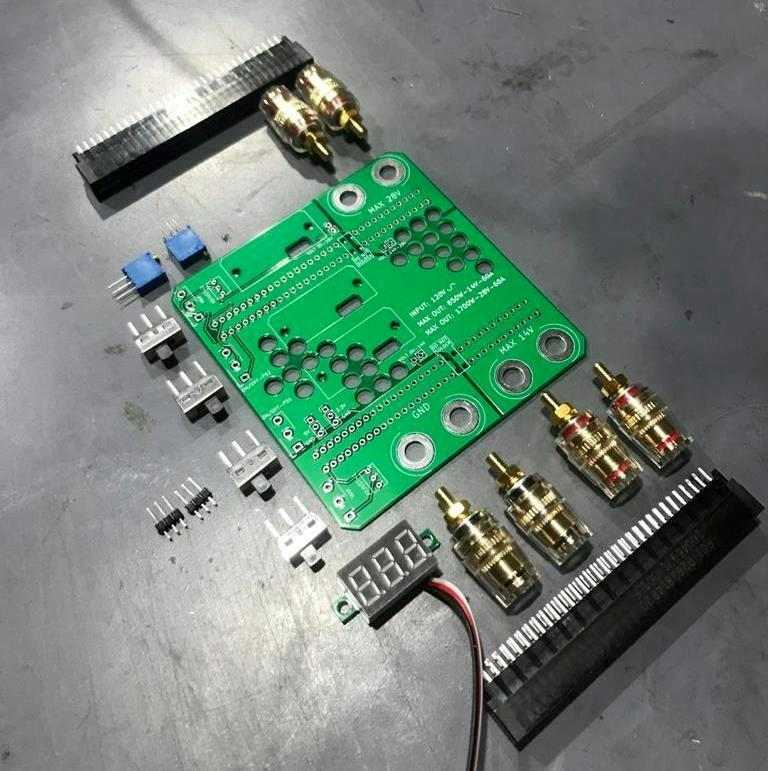
\includegraphics[width=441.9pt,height=443.5pt]{latexImage_395b7e877bb93ad8489aa48bc03c20d8.png}}
\end{picture}
\newpage
\begin{tikzpicture}[overlay]\path(0pt,0pt);\end{tikzpicture}
\begin{picture}(-5,0)(2.5,0)
\put(500.14,-727.616){\fontsize{12}{1}\usefont{T1}{ptm}{m}{n}\selectfont\color{color_29791}12}
\put(512.14,-727.616){\fontsize{12}{1}\usefont{T1}{ptm}{m}{n}\selectfont\color{color_29791} }
\put(515.14,-727.616){\fontsize{12}{1}\usefont{T1}{ptm}{m}{n}\selectfont\color{color_29791} }
\put(70.104,-742.496){\fontsize{10.56}{1}\usefont{T1}{ptm}{m}{n}\selectfont\color{color_29791} }
\put(72.744,-742.496){\fontsize{12}{1}\usefont{T1}{ptm}{m}{n}\selectfont\color{color_29791} }
\put(70.104,-72.09998){\fontsize{12}{1}\usefont{T1}{ptm}{m}{n}\selectfont\color{color_29791} }
\put(73.104,-72.09998){\fontsize{12}{1}\usefont{T1}{ptm}{m}{n}\selectfont\color{color_29791} }
\put(82.944,-87.21997){\fontsize{12}{1}\usefont{T1}{ptm}{m}{n}\selectfont\color{color_29791}總而言之}
\put(130.94,-87.21997){\fontsize{12}{1}\usefont{T1}{ptm}{m}{n}\selectfont\color{color_29791},}
\put(142.94,-87.21997){\fontsize{12}{1}\usefont{T1}{ptm}{m}{n}\selectfont\color{color_29791}其結果再次是對變革的控制和管理的更大需求}
\put(382.99,-87.21997){\fontsize{12}{1}\usefont{T1}{ptm}{m}{n}\selectfont\color{color_29791}。}
\put(394.99,-87.21997){\fontsize{12}{1}\usefont{T1}{ptm}{m}{n}\selectfont\color{color_29791}這意味著}
\put(442.99,-87.21997){\fontsize{12}{1}\usefont{T1}{ptm}{m}{n}\selectfont\color{color_29791}P}
\put(449.818,-87.21997){\fontsize{12}{1}\usefont{T1}{ptm}{m}{n}\selectfont\color{color_29791}L}
\put(456.898,-87.21997){\fontsize{12}{1}\usefont{T1}{ptm}{m}{n}\selectfont\color{color_29791}M}
\put(467.62,-87.21997){\fontsize{12}{1}\usefont{T1}{ptm}{m}{n}\selectfont\color{color_29791}-}
\put(69.384,-104.86){\fontsize{12}{1}\usefont{T1}{ptm}{m}{n}\selectfont\color{color_29791}MES}
\put(94.1,-104.86){\fontsize{12}{1}\usefont{T1}{ptm}{m}{n}\selectfont\color{color_29791}系統的實施將有很大説明}
\put(226.13,-104.86){\fontsize{12}{1}\usefont{T1}{ptm}{m}{n}\selectfont\color{color_29791}。}
\put(238.13,-104.86){\fontsize{12}{1}\usefont{T1}{ptm}{m}{n}\selectfont\color{color_29791}P}
\put(244.958,-104.86){\fontsize{12}{1}\usefont{T1}{ptm}{m}{n}\selectfont\color{color_29791}L}
\put(252.038,-104.86){\fontsize{12}{1}\usefont{T1}{ptm}{m}{n}\selectfont\color{color_29791}M}
\put(262.73,-104.86){\fontsize{12}{1}\usefont{T1}{ptm}{m}{n}\selectfont\color{color_29791}將需要在}
\put(310.838,-104.86){\fontsize{12}{1}\usefont{T1}{ptm}{m}{n}\selectfont\color{color_29791}小批量產品的整個生命週期中管理變}
\put(69.384,-122.5){\fontsize{12}{1}\usefont{T1}{ptm}{m}{n}\selectfont\color{color_29791}化和創新}
\put(117.38,-122.5){\fontsize{12}{1}\usefont{T1}{ptm}{m}{n}\selectfont\color{color_29791},}
\put(129.38,-122.5){\fontsize{12}{1}\usefont{T1}{ptm}{m}{n}\selectfont\color{color_29791}而}
\put(141.38,-122.5){\fontsize{12}{1}\usefont{T1}{ptm}{m}{n}\selectfont\color{color_29791}MES}
\put(166.1,-122.5){\fontsize{12}{1}\usefont{T1}{ptm}{m}{n}\selectfont\color{color_29791}將提供必要的即時反應和反饋}
\put(322.15,-122.5){\fontsize{12}{1}\usefont{T1}{ptm}{m}{n}\selectfont\color{color_29791},}
\put(334.15,-122.5){\fontsize{12}{1}\usefont{T1}{ptm}{m}{n}\selectfont\color{color_29791}以減少可能導致整個批次丟失的}
\put(69.384,-140.26){\fontsize{12}{1}\usefont{T1}{ptm}{m}{n}\selectfont\color{color_29791}錯誤}
\put(93.38,-140.26){\fontsize{12}{1}\usefont{T1}{ptm}{m}{n}\selectfont\color{color_29791}。}
\put(105.38,-140.26){\fontsize{12}{1}\usefont{T1}{ptm}{m}{n}\selectfont\color{color_29791} }
\put(108.38,-140.26){\fontsize{12}{1}\usefont{T1}{ptm}{m}{n}\selectfont\color{color_29791} }
\put(70.104,-157.66){\fontsize{12}{1}\usefont{T1}{ptm}{m}{n}\selectfont\color{color_29791} }
\put(73.104,-157.66){\fontsize{12}{1}\usefont{T1}{ptm}{m}{n}\selectfont\color{color_29791} }
\put(70.104,-173.38){\fontsize{12}{1}\usefont{T1}{ptm}{m}{n}\selectfont\color{color_29791} }
\put(73.104,-173.38){\fontsize{12}{1}\usefont{T1}{ptm}{m}{n}\selectfont\color{color_29791} }
\put(70.104,-194.02){\fontsize{12}{1}\usefont{T1}{ptm}{m}{n}\selectfont\color{color_29791} }
\put(73.104,-194.02){\fontsize{12}{1}\usefont{T1}{ptm}{m}{n}\selectfont\color{color_29791} }
\put(94.1,-194.02){\fontsize{15.96}{1}\usefont{T1}{ptm}{b}{n}\selectfont\color{color_29791} }
\put(98.06,-194.02){\fontsize{12}{1}\usefont{T1}{ptm}{m}{n}\selectfont\color{color_29791} }
\put(265.25,-212.98){\fontsize{15.96}{1}\usefont{T1}{ptm}{b}{n}\selectfont\color{color_29791}3}
\put(273.2779,-212.98){\fontsize{15.96}{1}\usefont{T1}{ptm}{b}{n}\selectfont\color{color_29791}. }
\put(281.21,-212.98){\fontsize{15.96}{1}\usefont{T1}{ptm}{m}{n}\selectfont\color{color_29791}章節}
\put(313.39,-212.98){\fontsize{15.96}{1}\usefont{T1}{ptm}{b}{n}\selectfont\color{color_29791}  }
\put(321.31,-212.98){\fontsize{12}{1}\usefont{T1}{ptm}{m}{n}\selectfont\color{color_29791} }
\put(90.98,-254.65){\fontsize{15.96}{1}\usefont{T1}{ptm}{b}{n}\selectfont\color{color_29791}PLM}
\put(126.491,-254.65){\fontsize{15.96}{1}\usefont{T1}{ptm}{b}{n}\selectfont\color{color_29791} }
\put(130.46,-254.65){\fontsize{15.96}{1}\usefont{T1}{ptm}{m}{n}\selectfont\color{color_29791}和}
\put(146.54,-254.65){\fontsize{15.96}{1}\usefont{T1}{ptm}{b}{n}\selectfont\color{color_29791} }
\put(150.5,-254.65){\fontsize{15.96}{1}\usefont{T1}{ptm}{b}{n}\selectfont\color{color_29791}M}
\put(165.5982,-254.65){\fontsize{15.96}{1}\usefont{T1}{ptm}{b}{n}\selectfont\color{color_29791}ES }
\put(189.17,-254.65){\fontsize{15.96}{1}\usefont{T1}{ptm}{m}{n}\selectfont\color{color_29791}的}
\put(205.2417,-254.65){\fontsize{15.96}{1}\usefont{T1}{ptm}{m}{n}\selectfont\color{color_29791}最}
\put(221.3134,-254.65){\fontsize{15.96}{1}\usefont{T1}{ptm}{m}{n}\selectfont\color{color_29791}新技}
\put(253.3452,-254.65){\fontsize{15.96}{1}\usefont{T1}{ptm}{m}{n}\selectfont\color{color_29791}術與}
\put(285.3769,-254.65){\fontsize{15.96}{1}\usefont{T1}{ptm}{m}{n}\selectfont\color{color_29791}整合}
\put(317.47,-254.65){\fontsize{15.96}{1}\usefont{T1}{ptm}{b}{n}\selectfont\color{color_29791} }
\put(321.43,-254.65){\fontsize{15.96}{1}\usefont{T1}{ptm}{b}{n}\selectfont\color{color_29791} }
\put(69.384,-288.97){\fontsize{12}{1}\usefont{T1}{ptm}{m}{n}\selectfont\color{color_29791}不幸的是}
\put(117.38,-288.97){\fontsize{12}{1}\usefont{T1}{ptm}{m}{n}\selectfont\color{color_29791},}
\put(129.38,-288.97){\fontsize{12}{1}\usefont{T1}{ptm}{m}{n}\selectfont\color{color_29791}關於}
\put(153.38,-288.97){\fontsize{12}{1}\usefont{T1}{ptm}{m}{n}\selectfont\color{color_29791}P}
\put(160.208,-288.97){\fontsize{12}{1}\usefont{T1}{ptm}{m}{n}\selectfont\color{color_29791}L}
\put(167.288,-288.97){\fontsize{12}{1}\usefont{T1}{ptm}{m}{n}\selectfont\color{color_29791}M}
\put(177.98,-288.97){\fontsize{12}{1}\usefont{T1}{ptm}{m}{n}\selectfont\color{color_29791}和}
\put(190.13,-288.97){\fontsize{12}{1}\usefont{T1}{ptm}{m}{n}\selectfont\color{color_29791}MES}
\put(214.85,-288.97){\fontsize{12}{1}\usefont{T1}{ptm}{m}{n}\selectfont\color{color_29791}系統之間集成的研究並不多}
\put(358.87,-288.97){\fontsize{12}{1}\usefont{T1}{ptm}{m}{n}\selectfont\color{color_29791}。}
\put(370.87,-288.97){\fontsize{12}{1}\usefont{T1}{ptm}{m}{n}\selectfont\color{color_29791}但是}
\put(394.87,-288.97){\fontsize{12}{1}\usefont{T1}{ptm}{m}{n}\selectfont\color{color_29791},}
\put(406.87,-288.97){\fontsize{12}{1}\usefont{T1}{ptm}{m}{n}\selectfont\color{color_29791}對於上述整合的最}
\put(69.384,-306.73){\fontsize{12}{1}\usefont{T1}{ptm}{m}{n}\selectfont\color{color_29791}可能影響}
\put(117.38,-306.73){\fontsize{12}{1}\usefont{T1}{ptm}{m}{n}\selectfont\color{color_29791},}
\put(129.38,-306.73){\fontsize{12}{1}\usefont{T1}{ptm}{m}{n}\selectfont\color{color_29791}似乎達成了共識}
\put(213.41,-306.73){\fontsize{12}{1}\usefont{T1}{ptm}{m}{n}\selectfont\color{color_29791}。}
\put(225.41,-306.73){\fontsize{12}{1}\usefont{T1}{ptm}{m}{n}\selectfont\color{color_29791}這些是同步和更嚴格的公差}
\put(369.43,-306.73){\fontsize{12}{1}\usefont{T1}{ptm}{m}{n}\selectfont\color{color_29791}。}
\put(381.43,-306.73){\fontsize{12}{1}\usefont{T1}{ptm}{m}{n}\selectfont\color{color_29791}  }
\put(387.43,-306.73){\fontsize{12}{1}\usefont{T1}{ptm}{m}{n}\selectfont\color{color_29791} }
\put(70.104,-324.13){\fontsize{12}{1}\usefont{T1}{ptm}{m}{n}\selectfont\color{color_29791} }
\put(73.104,-324.13){\fontsize{12}{1}\usefont{T1}{ptm}{m}{n}\selectfont\color{color_29791} }
\put(69.384,-340.09){\fontsize{12}{1}\usefont{T1}{ptm}{m}{n}\selectfont\color{color_29791}正如}
\put(93.38,-340.09){\fontsize{12}{1}\usefont{T1}{ptm}{m}{n}\selectfont\color{color_29791}D'}
\put(104.06,-340.09){\fontsize{12}{1}\usefont{T1}{ptm}{m}{n}\selectfont\color{color_29791}Antonio}
\put(143.42,-340.09){\fontsize{12}{1}\usefont{T1}{ptm}{m}{n}\selectfont\color{color_29791}等人}
\put(167.42,-340.09){\fontsize{12}{1}\usefont{T1}{ptm}{m}{n}\selectfont\color{color_29791}(}
\put(179.42,-340.09){\fontsize{12}{1}\usefont{T1}{ptm}{m}{n}\selectfont\color{color_29791}20}
\put(191.528,-340.09){\fontsize{12}{1}\usefont{T1}{ptm}{m}{n}\selectfont\color{color_29791}15}
\put(203.57,-340.09){\fontsize{12}{1}\usefont{T1}{ptm}{m}{n}\selectfont\color{color_29791}年}
\put(215.57,-340.09){\fontsize{12}{1}\usefont{T1}{ptm}{m}{n}\selectfont\color{color_29791})}
\put(227.57,-340.09){\fontsize{12}{1}\usefont{T1}{ptm}{m}{n}\selectfont\color{color_29791}所解釋的那樣}
\put(299.57,-340.09){\fontsize{12}{1}\usefont{T1}{ptm}{m}{n}\selectfont\color{color_29791},}
\put(311.57,-340.09){\fontsize{12}{1}\usefont{T1}{ptm}{m}{n}\selectfont\color{color_29791}該案例研究側重於涉及航空應用精密}
\put(69.384,-357.73){\fontsize{12}{1}\usefont{T1}{ptm}{m}{n}\selectfont\color{color_29791}部件製造的案例研究}
\put(177.38,-357.73){\fontsize{12}{1}\usefont{T1}{ptm}{m}{n}\selectfont\color{color_29791},}
\put(189.41,-357.73){\fontsize{12}{1}\usefont{T1}{ptm}{m}{n}\selectfont\color{color_29791}部署監測和控制系統的第一個優勢是產品品質的提高}
\put(465.46,-357.73){\fontsize{12}{1}\usefont{T1}{ptm}{m}{n}\selectfont\color{color_29791}:}
\put(477.46,-357.73){\fontsize{12}{1}\usefont{T1}{ptm}{m}{n}\selectfont\color{color_29791}感測}
\put(69.384,-375.49){\fontsize{12}{1}\usefont{T1}{ptm}{m}{n}\selectfont\color{color_29791}器允許檢測}
\put(129.38,-375.49){\fontsize{12}{1}\usefont{T1}{ptm}{m}{n}\selectfont\color{color_29791},}
\put(141.38,-375.49){\fontsize{12}{1}\usefont{T1}{ptm}{m}{n}\selectfont\color{color_29791}測量和監測影響過程性能或產品品質的變數}
\put(369.43,-375.49){\fontsize{12}{1}\usefont{T1}{ptm}{m}{n}\selectfont\color{color_29791},}
\put(381.43,-375.49){\fontsize{12}{1}\usefont{T1}{ptm}{m}{n}\selectfont\color{color_29791}事件和情況}
\put(441.43,-375.49){\fontsize{12}{1}\usefont{T1}{ptm}{m}{n}\selectfont\color{color_29791}。}
\put(453.46,-375.49){\fontsize{12}{1}\usefont{T1}{ptm}{m}{n}\selectfont\color{color_29791} }
\put(456.46,-375.49){\fontsize{12}{1}\usefont{T1}{ptm}{m}{n}\selectfont\color{color_29791} }
\put(70.104,-392.89){\fontsize{12}{1}\usefont{T1}{ptm}{m}{n}\selectfont\color{color_29791} }
\put(73.104,-392.89){\fontsize{12}{1}\usefont{T1}{ptm}{m}{n}\selectfont\color{color_29791} }
\put(82.944,-408.85){\fontsize{12}{1}\usefont{T1}{ptm}{m}{n}\selectfont\color{color_29791}將}
\put(94.94,-408.85){\fontsize{12}{1}\usefont{T1}{ptm}{m}{n}\selectfont\color{color_29791} }
\put(487.78,-408.85){\fontsize{12}{1}\usefont{T1}{ptm}{m}{n}\selectfont\color{color_29791}P}
\put(494.608,-408.85){\fontsize{12}{1}\usefont{T1}{ptm}{m}{n}\selectfont\color{color_29791}L}
\put(501.688,-408.85){\fontsize{12}{1}\usefont{T1}{ptm}{m}{n}\selectfont\color{color_29791}M}
\put(512.476,-408.85){\fontsize{12}{1}\usefont{T1}{ptm}{m}{n}\selectfont\color{color_29791} }
\put(69.384,-426.51){\fontsize{12}{1}\usefont{T1}{ptm}{m}{n}\selectfont\color{color_29791}與任何其他系統整合的核心問題之一圍繞著資訊的擁有權}
\put(369.43,-426.51){\fontsize{12}{1}\usefont{T1}{ptm}{m}{n}\selectfont\color{color_29791}。}
\put(381.43,-426.51){\fontsize{12}{1}\usefont{T1}{ptm}{m}{n}\selectfont\color{color_29791}一個可能的解決方案依}
\put(69.384,-444.15){\fontsize{12}{1}\usefont{T1}{ptm}{m}{n}\selectfont\color{color_29791}賴於資料庫集成以及系}
\put(189.41,-444.15){\fontsize{12}{1}\usefont{T1}{ptm}{m}{n}\selectfont\color{color_29791}統之間的中間件的使用}
\put(309.41,-444.15){\fontsize{12}{1}\usefont{T1}{ptm}{m}{n}\selectfont\color{color_29791}。}
\put(321.43,-444.15){\fontsize{12}{1}\usefont{T1}{ptm}{m}{n}\selectfont\color{color_29791}正如}
\put(345.43,-444.15){\fontsize{12}{1}\usefont{T1}{ptm}{m}{n}\selectfont\color{color_29791}S}
\put(352.138,-444.15){\fontsize{12}{1}\usefont{T1}{ptm}{m}{n}\selectfont\color{color_29791}a}
\put(357.418,-444.15){\fontsize{12}{1}\usefont{T1}{ptm}{m}{n}\selectfont\color{color_29791}a}
\put(362.698,-444.15){\fontsize{12}{1}\usefont{T1}{ptm}{m}{n}\selectfont\color{color_29791}ksvuori}
\put(398.71,-444.15){\fontsize{12}{1}\usefont{T1}{ptm}{m}{n}\selectfont\color{color_29791}和}
\put(410.83,-444.15){\fontsize{12}{1}\usefont{T1}{ptm}{m}{n}\selectfont\color{color_29791}I}
\put(414.67,-444.15){\fontsize{12}{1}\usefont{T1}{ptm}{m}{n}\selectfont\color{color_29791}m}
\put(424.138,-444.15){\fontsize{12}{1}\usefont{T1}{ptm}{m}{n}\selectfont\color{color_29791}monen}
\put(456.82,-444.15){\fontsize{12}{1}\usefont{T1}{ptm}{m}{n}\selectfont\color{color_29791}(}
\put(468.82,-444.15){\fontsize{12}{1}\usefont{T1}{ptm}{m}{n}\selectfont\color{color_29791}2008}
\put(492.82,-444.15){\fontsize{12}{1}\usefont{T1}{ptm}{m}{n}\selectfont\color{color_29791})}
\put(69.384,-461.79){\fontsize{12}{1}\usefont{T1}{ptm}{m}{n}\selectfont\color{color_29791}所寫的那樣}
\put(129.38,-461.79){\fontsize{12}{1}\usefont{T1}{ptm}{m}{n}\selectfont\color{color_29791}。}
\put(141.38,-461.79){\fontsize{12}{1}\usefont{T1}{ptm}{m}{n}\selectfont\color{color_29791}一個合理的目標是資訊應始終在一個地方更新}
\put(381.43,-461.79){\fontsize{12}{1}\usefont{T1}{ptm}{m}{n}\selectfont\color{color_29791}。}
\put(393.43,-461.79){\fontsize{12}{1}\usefont{T1}{ptm}{m}{n}\selectfont\color{color_29791}其他系統可以直接從}
\put(501.46,-461.79){\fontsize{12}{1}\usefont{T1}{ptm}{m}{n}\selectfont\color{color_29791} }
\put(69.384,-479.19){\fontsize{12}{1}\usefont{T1}{ptm}{m}{n}\selectfont\color{color_29791}P}
\put(76.21201,-479.19){\fontsize{12}{1}\usefont{T1}{ptm}{m}{n}\selectfont\color{color_29791}L}
\put(83.29201,-479.19){\fontsize{12}{1}\usefont{T1}{ptm}{m}{n}\selectfont\color{color_29791}M }
\put(69.384,-494.91){\fontsize{12}{1}\usefont{T1}{ptm}{m}{n}\selectfont\color{color_29791}資料庫中讀取資訊}
\put(165.38,-494.91){\fontsize{12}{1}\usefont{T1}{ptm}{m}{n}\selectfont\color{color_29791},}
\put(177.38,-494.91){\fontsize{12}{1}\usefont{T1}{ptm}{m}{n}\selectfont\color{color_29791}如有必要}
\put(225.41,-494.91){\fontsize{12}{1}\usefont{T1}{ptm}{m}{n}\selectfont\color{color_29791},}
\put(237.41,-494.91){\fontsize{12}{1}\usefont{T1}{ptm}{m}{n}\selectfont\color{color_29791}可以在其他系統的資料庫上複製所需的資訊}
\put(465.46,-494.91){\fontsize{12}{1}\usefont{T1}{ptm}{m}{n}\selectfont\color{color_29791},}
\put(477.46,-494.91){\fontsize{12}{1}\usefont{T1}{ptm}{m}{n}\selectfont\color{color_29791}如圖}
\put(501.46,-494.91){\fontsize{12}{1}\usefont{T1}{ptm}{m}{n}\selectfont\color{color_29791} }
\put(506.62,-494.91){\fontsize{12}{1}\usefont{T1}{ptm}{m}{n}\selectfont\color{color_29791}7 }
\put(69.384,-512.55){\fontsize{12}{1}\usefont{T1}{ptm}{m}{n}\selectfont\color{color_29791}所示}
\put(93.38,-512.55){\fontsize{12}{1}\usefont{T1}{ptm}{m}{n}\selectfont\color{color_29791}。}
\put(105.38,-512.55){\fontsize{12}{1}\usefont{T1}{ptm}{m}{n}\selectfont\color{color_29791}雖然它主要從}
\put(177.38,-512.55){\fontsize{12}{1}\usefont{T1}{ptm}{m}{n}\selectfont\color{color_29791}P}
\put(184.208,-512.55){\fontsize{12}{1}\usefont{T1}{ptm}{m}{n}\selectfont\color{color_29791}L}
\put(191.408,-512.55){\fontsize{12}{1}\usefont{T1}{ptm}{m}{n}\selectfont\color{color_29791}M}
\put(202.13,-512.55){\fontsize{12}{1}\usefont{T1}{ptm}{m}{n}\selectfont\color{color_29791}-}
\put(206.09,-512.55){\fontsize{12}{1}\usefont{T1}{ptm}{m}{n}\selectfont\color{color_29791}ERP}
\put(228.17,-512.55){\fontsize{12}{1}\usefont{T1}{ptm}{m}{n}\selectfont\color{color_29791}集成的角度指出了這一點}
\put(360.19,-512.55){\fontsize{12}{1}\usefont{T1}{ptm}{m}{n}\selectfont\color{color_29791},}
\put(372.19,-512.55){\fontsize{12}{1}\usefont{T1}{ptm}{m}{n}\selectfont\color{color_29791}但從}
\put(396.19,-512.55){\fontsize{12}{1}\usefont{T1}{ptm}{m}{n}\selectfont\color{color_29791}P}
\put(403.018,-512.55){\fontsize{12}{1}\usefont{T1}{ptm}{m}{n}\selectfont\color{color_29791}L}
\put(410.098,-512.55){\fontsize{12}{1}\usefont{T1}{ptm}{m}{n}\selectfont\color{color_29791}M}
\put(420.79,-512.55){\fontsize{12}{1}\usefont{T1}{ptm}{m}{n}\selectfont\color{color_29791}-}
\put(69.384,-530.19){\fontsize{12}{1}\usefont{T1}{ptm}{m}{n}\selectfont\color{color_29791}MES}
\put(94.1,-530.19){\fontsize{12}{1}\usefont{T1}{ptm}{m}{n}\selectfont\color{color_29791}集成的角度來看}
\put(178.1,-530.19){\fontsize{12}{1}\usefont{T1}{ptm}{m}{n}\selectfont\color{color_29791},}
\put(190.13,-530.19){\fontsize{12}{1}\usefont{T1}{ptm}{m}{n}\selectfont\color{color_29791}它仍然非常有價值}
\put(286.13,-530.19){\fontsize{12}{1}\usefont{T1}{ptm}{m}{n}\selectfont\color{color_29791},}
\put(298.13,-530.19){\fontsize{12}{1}\usefont{T1}{ptm}{m}{n}\selectfont\color{color_29791}因為它是一個例子}
\put(394.15,-530.19){\fontsize{12}{1}\usefont{T1}{ptm}{m}{n}\selectfont\color{color_29791},}
\put(406.15,-530.19){\fontsize{12}{1}\usefont{T1}{ptm}{m}{n}\selectfont\color{color_29791}說明如何通過圍繞}
\put(69.384,-547.95){\fontsize{12}{1}\usefont{T1}{ptm}{m}{n}\selectfont\color{color_29791}將不同性質的檔載入到集中式}
\put(225.41,-547.95){\fontsize{12}{1}\usefont{T1}{ptm}{m}{n}\selectfont\color{color_29791}P}
\put(232.238,-547.95){\fontsize{12}{1}\usefont{T1}{ptm}{m}{n}\selectfont\color{color_29791}L}
\put(239.318,-547.95){\fontsize{12}{1}\usefont{T1}{ptm}{m}{n}\selectfont\color{color_29791}M}
\put(250.01,-547.95){\fontsize{12}{1}\usefont{T1}{ptm}{m}{n}\selectfont\color{color_29791}-}
\put(253.97,-547.95){\fontsize{12}{1}\usefont{T1}{ptm}{m}{n}\selectfont\color{color_29791}ERP}
\put(276.05,-547.95){\fontsize{12}{1}\usefont{T1}{ptm}{m}{n}\selectfont\color{color_29791}系統中的系統來期望更好的操作}
\put(444.07,-547.95){\fontsize{12}{1}\usefont{T1}{ptm}{m}{n}\selectfont\color{color_29791}。}
\put(456.1,-547.95){\fontsize{12}{1}\usefont{T1}{ptm}{m}{n}\selectfont\color{color_29791} }
\put(459.1,-547.95){\fontsize{12}{1}\usefont{T1}{ptm}{m}{n}\selectfont\color{color_29791} }
\put(84.264,-565.47){\fontsize{12}{1}\usefont{T1}{ptm}{m}{n}\selectfont\color{color_29791} }
\put(87.26,-565.47){\fontsize{12}{1}\usefont{T1}{ptm}{m}{n}\selectfont\color{color_29791} }
\put(474.22,-691.496){\fontsize{12}{1}\usefont{T1}{ptm}{m}{n}\selectfont\color{color_29791} }
\put(477.22,-691.496){\fontsize{12}{1}\usefont{T1}{ptm}{m}{n}\selectfont\color{color_29791} }
\put(134.06,-703.856){\fontsize{12}{1}\usefont{T1}{ptm}{m}{n}\selectfont\color{color_29791}圖}
\put(146.18,-703.856){\fontsize{12}{1}\usefont{T1}{ptm}{b}{n}\selectfont\color{color_29791} }
\put(149.18,-703.856){\fontsize{12}{1}\usefont{T1}{ptm}{b}{n}\selectfont\color{color_29791}7 }
\put(158.18,-703.856){\fontsize{12}{1}\usefont{T1}{ptm}{b}{n}\selectfont\color{color_29791}P}
\put(165.38,-703.856){\fontsize{12}{1}\usefont{T1}{ptm}{b}{n}\selectfont\color{color_29791}L}
\put(173.408,-703.856){\fontsize{12}{1}\usefont{T1}{ptm}{b}{n}\selectfont\color{color_29791}M}
\put(184.688,-703.856){\fontsize{12}{1}\usefont{T1}{ptm}{b}{n}\selectfont\color{color_29791} }
\put(187.73,-703.856){\fontsize{12}{1}\usefont{T1}{ptm}{m}{n}\selectfont\color{color_29791}集}
\put(199.838,-703.856){\fontsize{12}{1}\usefont{T1}{ptm}{m}{n}\selectfont\color{color_29791}成示意圖}
\put(247.85,-703.856){\fontsize{12}{1}\usefont{T1}{ptm}{m}{n}\selectfont\color{color_29791}(}
\put(259.97,-703.856){\fontsize{12}{1}\usefont{T1}{ptm}{b}{n}\selectfont\color{color_29791}S}
\put(266.678,-703.856){\fontsize{12}{1}\usefont{T1}{ptm}{b}{n}\selectfont\color{color_29791}aa}
\put(278.558,-703.856){\fontsize{12}{1}\usefont{T1}{ptm}{b}{n}\selectfont\color{color_29791}k}
\put(285.266,-703.856){\fontsize{12}{1}\usefont{T1}{ptm}{b}{n}\selectfont\color{color_29791}svu}
\put(302.654,-703.856){\fontsize{12}{1}\usefont{T1}{ptm}{b}{n}\selectfont\color{color_29791}or}
\put(313.934,-703.856){\fontsize{12}{1}\usefont{T1}{ptm}{b}{n}\selectfont\color{color_29791}i }
\put(320.23,-703.856){\fontsize{12}{1}\usefont{T1}{ptm}{m}{n}\selectfont\color{color_29791}和}
\put(332.35,-703.856){\fontsize{12}{1}\usefont{T1}{ptm}{b}{n}\selectfont\color{color_29791} }
\put(335.35,-703.856){\fontsize{12}{1}\usefont{T1}{ptm}{b}{n}\selectfont\color{color_29791}Imm}
\put(359.83,-703.856){\fontsize{12}{1}\usefont{T1}{ptm}{b}{n}\selectfont\color{color_29791}o}
\put(365.938,-703.856){\fontsize{12}{1}\usefont{T1}{ptm}{b}{n}\selectfont\color{color_29791}n}
\put(372.646,-703.856){\fontsize{12}{1}\usefont{T1}{ptm}{b}{n}\selectfont\color{color_29791}e}
\put(377.926,-703.856){\fontsize{12}{1}\usefont{T1}{ptm}{b}{n}\selectfont\color{color_29791}n}
\put(384.67,-703.856){\fontsize{12}{1}\usefont{T1}{ptm}{m}{n}\selectfont\color{color_29791},}
\put(396.79,-703.856){\fontsize{12}{1}\usefont{T1}{ptm}{b}{n}\selectfont\color{color_29791}2008 }
\put(423.67,-703.856){\fontsize{12}{1}\usefont{T1}{ptm}{m}{n}\selectfont\color{color_29791}年}
\put(435.67,-703.856){\fontsize{12}{1}\usefont{T1}{ptm}{m}{n}\selectfont\color{color_29791})}
\put(447.82,-703.856){\fontsize{12}{1}\usefont{T1}{ptm}{b}{n}\selectfont\color{color_29791} }
\put(450.7,-703.856){\fontsize{12}{1}\usefont{T1}{ptm}{m}{n}\selectfont\color{color_29791} }
\put(114.15,-691.311){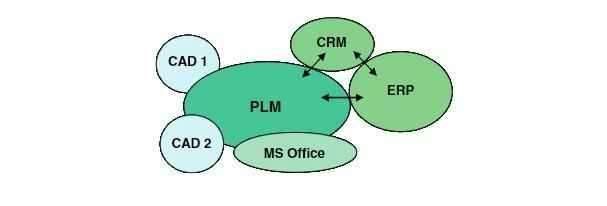
\includegraphics[width=359.95pt,height=122.24pt]{latexImage_0cdc990ef95f4f8f0c226939fa11cc69.png}}
\end{picture}
\newpage
\begin{tikzpicture}[overlay]\path(0pt,0pt);\end{tikzpicture}
\begin{picture}(-5,0)(2.5,0)
\put(500.14,-727.616){\fontsize{12}{1}\usefont{T1}{ptm}{m}{n}\selectfont\color{color_29791}13}
\put(512.14,-727.616){\fontsize{12}{1}\usefont{T1}{ptm}{m}{n}\selectfont\color{color_29791} }
\put(515.14,-727.616){\fontsize{12}{1}\usefont{T1}{ptm}{m}{n}\selectfont\color{color_29791} }
\put(70.104,-742.496){\fontsize{10.56}{1}\usefont{T1}{ptm}{m}{n}\selectfont\color{color_29791} }
\put(72.744,-742.496){\fontsize{12}{1}\usefont{T1}{ptm}{m}{n}\selectfont\color{color_29791} }
\put(70.104,-72.09998){\fontsize{12}{1}\usefont{T1}{ptm}{m}{n}\selectfont\color{color_29791} }
\put(73.104,-72.09998){\fontsize{12}{1}\usefont{T1}{ptm}{m}{n}\selectfont\color{color_29791} }
\put(82.944,-87.09998){\fontsize{11.04}{1}\usefont{T1}{uarial}{m}{n}\selectfont\color{color_137925} }
\put(69.384,-102.46){\fontsize{12}{1}\usefont{T1}{ptm}{m}{n}\selectfont\color{color_29791}因此}
\put(93.38,-102.46){\fontsize{12}{1}\usefont{T1}{ptm}{m}{n}\selectfont\color{color_29791},}
\put(105.38,-102.46){\fontsize{12}{1}\usefont{T1}{ptm}{m}{n}\selectfont\color{color_29791}中間件將是一個軟體框架}
\put(237.41,-102.46){\fontsize{12}{1}\usefont{T1}{ptm}{m}{n}\selectfont\color{color_29791},}
\put(249.41,-102.46){\fontsize{12}{1}\usefont{T1}{ptm}{m}{n}\selectfont\color{color_29791}以使用者友好的方式組織和連接提供給系統資料}
\put(69.384,-120.1){\fontsize{12}{1}\usefont{T1}{ptm}{m}{n}\selectfont\color{color_29791}庫的所有資訊}
\put(141.38,-120.1){\fontsize{12}{1}\usefont{T1}{ptm}{m}{n}\selectfont\color{color_29791}。}
\put(153.38,-120.1){\fontsize{12}{1}\usefont{T1}{ptm}{m}{n}\selectfont\color{color_29791}這種應用程式也稱為集成應用程式}
\put(333.43,-120.1){\fontsize{12}{1}\usefont{T1}{ptm}{m}{n}\selectfont\color{color_29791},}
\put(345.43,-120.1){\fontsize{12}{1}\usefont{T1}{ptm}{m}{n}\selectfont\color{color_29791}正如}
\put(369.43,-120.1){\fontsize{12}{1}\usefont{T1}{ptm}{m}{n}\selectfont\color{color_29791}S}
\put(376.138,-120.1){\fontsize{12}{1}\usefont{T1}{ptm}{m}{n}\selectfont\color{color_29791}tar}
\put(388.738,-120.1){\fontsize{12}{1}\usefont{T1}{ptm}{m}{n}\selectfont\color{color_29791}k}
\put(394.75,-120.1){\fontsize{12}{1}\usefont{T1}{ptm}{m}{n}\selectfont\color{color_29791}(}
\put(406.75,-120.1){\fontsize{12}{1}\usefont{T1}{ptm}{m}{n}\selectfont\color{color_29791}2015}
\put(430.75,-120.1){\fontsize{12}{1}\usefont{T1}{ptm}{m}{n}\selectfont\color{color_29791})}
\put(442.75,-120.1){\fontsize{12}{1}\usefont{T1}{ptm}{m}{n}\selectfont\color{color_29791}所指出的那}
\put(69.384,-137.74){\fontsize{12}{1}\usefont{T1}{ptm}{m}{n}\selectfont\color{color_29791}樣}
\put(81.384,-137.74){\fontsize{12}{1}\usefont{T1}{ptm}{m}{n}\selectfont\color{color_29791},}
\put(93.38,-137.74){\fontsize{12}{1}\usefont{T1}{ptm}{m}{n}\selectfont\color{color_29791}這些應用程式支援在}
\put(201.41,-137.74){\fontsize{12}{1}\usefont{T1}{ptm}{m}{n}\selectfont\color{color_29791}P}
\put(208.238,-137.74){\fontsize{12}{1}\usefont{T1}{ptm}{m}{n}\selectfont\color{color_29791}L}
\put(215.318,-137.74){\fontsize{12}{1}\usefont{T1}{ptm}{m}{n}\selectfont\color{color_29791}M}
\put(226.01,-137.74){\fontsize{12}{1}\usefont{T1}{ptm}{m}{n}\selectfont\color{color_29791}應用程式之間交}
\put(310.118,-137.74){\fontsize{12}{1}\usefont{T1}{ptm}{m}{n}\selectfont\color{color_29791}換產品資訊}
\put(370.15,-137.74){\fontsize{12}{1}\usefont{T1}{ptm}{m}{n}\selectfont\color{color_29791}(}
\put(382.15,-137.74){\fontsize{12}{1}\usefont{T1}{ptm}{m}{n}\selectfont\color{color_29791}例如}
\put(406.15,-137.74){\fontsize{12}{1}\usefont{T1}{ptm}{m}{n}\selectfont\color{color_29791},}
\put(418.15,-137.74){\fontsize{12}{1}\usefont{T1}{ptm}{m}{n}\selectfont\color{color_29791}C}
\put(426.178,-137.74){\fontsize{12}{1}\usefont{T1}{ptm}{m}{n}\selectfont\color{color_29791}AD}
\put(443.47,-137.74){\fontsize{12}{1}\usefont{T1}{ptm}{m}{n}\selectfont\color{color_29791}應用程式和}
\put(503.5,-137.74){\fontsize{12}{1}\usefont{T1}{ptm}{m}{n}\selectfont\color{color_29791}C}
\put(69.384,-155.38){\fontsize{12}{1}\usefont{T1}{ptm}{m}{n}\selectfont\color{color_29791}AE}
\put(85.34,-155.38){\fontsize{12}{1}\usefont{T1}{ptm}{m}{n}\selectfont\color{color_29791}應用程式之間}
\put(157.34,-155.38){\fontsize{12}{1}\usefont{T1}{ptm}{m}{n}\selectfont\color{color_29791})。}
\put(181.37,-155.38){\fontsize{12}{1}\usefont{T1}{ptm}{m}{n}\selectfont\color{color_29791}它們還支援在}
\put(253.37,-155.38){\fontsize{12}{1}\usefont{T1}{ptm}{m}{n}\selectfont\color{color_29791} }
\put(258.53,-155.38){\fontsize{12}{1}\usefont{T1}{ptm}{m}{n}\selectfont\color{color_29791}P}
\put(265.358,-155.38){\fontsize{12}{1}\usefont{T1}{ptm}{m}{n}\selectfont\color{color_29791}L}
\put(272.438,-155.38){\fontsize{12}{1}\usefont{T1}{ptm}{m}{n}\selectfont\color{color_29791}M}
\put(283.226,-155.38){\fontsize{12}{1}\usefont{T1}{ptm}{m}{n}\selectfont\color{color_29791} }
\put(288.41,-155.38){\fontsize{12}{1}\usefont{T1}{ptm}{m}{n}\selectfont\color{color_29791}應}
\put(300.518,-155.38){\fontsize{12}{1}\usefont{T1}{ptm}{m}{n}\selectfont\color{color_29791}用程式和其他企業應用程式}
\put(444.55,-155.38){\fontsize{12}{1}\usefont{T1}{ptm}{m}{n}\selectfont\color{color_29791}(}
\put(456.58,-155.38){\fontsize{12}{1}\usefont{T1}{ptm}{m}{n}\selectfont\color{color_29791}如}
\put(468.58,-155.38){\fontsize{12}{1}\usefont{T1}{ptm}{m}{n}\selectfont\color{color_29791} }
\put(473.74,-155.38){\fontsize{12}{1}\usefont{T1}{ptm}{m}{n}\selectfont\color{color_29791}ERP}
\put(495.34,-155.38){\fontsize{12}{1}\usefont{T1}{ptm}{m}{n}\selectfont\color{color_29791} }
\put(500.5,-155.38){\fontsize{12}{1}\usefont{T1}{ptm}{m}{n}\selectfont\color{color_29791}和}
\put(512.5,-155.38){\fontsize{12}{1}\usefont{T1}{ptm}{m}{n}\selectfont\color{color_29791} }
\put(69.384,-173.02){\fontsize{12}{1}\usefont{T1}{ptm}{m}{n}\selectfont\color{color_29791}CRM}
\put(96.14,-173.02){\fontsize{12}{1}\usefont{T1}{ptm}{m}{n}\selectfont\color{color_29791})}
\put(108.14,-173.02){\fontsize{12}{1}\usefont{T1}{ptm}{m}{n}\selectfont\color{color_29791}之間交換產品資}
\put(192.02,-173.02){\fontsize{12}{1}\usefont{T1}{ptm}{m}{n}\selectfont\color{color_29791}訊}
\put(204.05,-173.02){\fontsize{12}{1}\usefont{T1}{ptm}{m}{n}\selectfont\color{color_29791}。}
\put(216.05,-173.02){\fontsize{12}{1}\usefont{T1}{ptm}{m}{n}\selectfont\color{color_29791} }
\put(219.05,-173.02){\fontsize{12}{1}\usefont{T1}{ptm}{m}{n}\selectfont\color{color_29791} }
\put(84.264,-190.54){\fontsize{12}{1}\usefont{T1}{ptm}{m}{n}\selectfont\color{color_29791} }
\put(87.26,-190.54){\fontsize{12}{1}\usefont{T1}{ptm}{m}{n}\selectfont\color{color_29791} }
\put(82.944,-206.5){\fontsize{12}{1}\usefont{T1}{ptm}{m}{n}\selectfont\color{color_29791}以一種非常相關的方式}
\put(202.97,-206.5){\fontsize{12}{1}\usefont{T1}{ptm}{m}{n}\selectfont\color{color_29791},}
\put(214.97,-206.5){\fontsize{12}{1}\usefont{T1}{ptm}{m}{n}\selectfont\color{color_29791}這種中間件思路得到了擴展}
\put(358.99,-206.5){\fontsize{12}{1}\usefont{T1}{ptm}{m}{n}\selectfont\color{color_29791}(}
\put(370.99,-206.5){\fontsize{12}{1}\usefont{T1}{ptm}{m}{n}\selectfont\color{color_29791}B}
\put(378.91,-206.5){\fontsize{12}{1}\usefont{T1}{ptm}{m}{n}\selectfont\color{color_29791}e}
\put(384.19,-206.5){\fontsize{12}{1}\usefont{T1}{ptm}{m}{n}\selectfont\color{color_29791}n }
\put(406.378,-206.5){\fontsize{12}{1}\usefont{T1}{ptm}{m}{n}\selectfont\color{color_29791}Khe}
\put(426.298,-206.5){\fontsize{12}{1}\usefont{T1}{ptm}{m}{n}\selectfont\color{color_29791}dh}
\put(438.406,-206.5){\fontsize{12}{1}\usefont{T1}{ptm}{m}{n}\selectfont\color{color_29791}e}
\put(443.794,-206.5){\fontsize{12}{1}\usefont{T1}{ptm}{m}{n}\selectfont\color{color_29791}r }
\put(463.942,-206.5){\fontsize{12}{1}\usefont{T1}{ptm}{m}{n}\selectfont\color{color_29791}e}
\put(469.222,-206.5){\fontsize{12}{1}\usefont{T1}{ptm}{m}{n}\selectfont\color{color_29791}t }
\put(488.77,-206.5){\fontsize{12}{1}\usefont{T1}{ptm}{m}{n}\selectfont\color{color_29791}a}
\put(494.05,-206.5){\fontsize{12}{1}\usefont{T1}{ptm}{m}{n}\selectfont\color{color_29791}l.}
\put(500.5,-206.5){\fontsize{12}{1}\usefont{T1}{ptm}{m}{n}\selectfont\color{color_29791},}
\put(512.5,-206.5){\fontsize{12}{1}\usefont{T1}{ptm}{m}{n}\selectfont\color{color_29791} }
\put(69.384,-224.14){\fontsize{12}{1}\usefont{T1}{ptm}{m}{n}\selectfont\color{color_29791}2011}
\put(93.38,-224.14){\fontsize{12}{1}\usefont{T1}{ptm}{m}{n}\selectfont\color{color_29791})。}
\put(117.38,-224.14){\fontsize{12}{1}\usefont{T1}{ptm}{m}{n}\selectfont\color{color_29791}在他們關於實現集成}
\put(225.41,-224.14){\fontsize{12}{1}\usefont{T1}{ptm}{m}{n}\selectfont\color{color_29791}MES}
\put(250.118,-224.14){\fontsize{12}{1}\usefont{T1}{ptm}{m}{n}\selectfont\color{color_29791}+}
\put(256.838,-224.14){\fontsize{12}{1}\usefont{T1}{ptm}{m}{n}\selectfont\color{color_29791}P}
\put(263.666,-224.14){\fontsize{12}{1}\usefont{T1}{ptm}{m}{n}\selectfont\color{color_29791}L}
\put(270.746,-224.14){\fontsize{12}{1}\usefont{T1}{ptm}{m}{n}\selectfont\color{color_29791}M}
\put(281.45,-224.14){\fontsize{12}{1}\usefont{T1}{ptm}{m}{n}\selectfont\color{color_29791}的不}
\put(305.558,-224.14){\fontsize{12}{1}\usefont{T1}{ptm}{m}{n}\selectfont\color{color_29791}同系統架構的工作中}
\put(413.59,-224.14){\fontsize{12}{1}\usefont{T1}{ptm}{m}{n}\selectfont\color{color_29791},}
\put(425.59,-224.14){\fontsize{12}{1}\usefont{T1}{ptm}{m}{n}\selectfont\color{color_29791}他們描述了中介}
\put(69.384,-241.66){\fontsize{12}{1}\usefont{T1}{ptm}{m}{n}\selectfont\color{color_29791}系統在}
\put(105.38,-241.66){\fontsize{12}{1}\usefont{T1}{ptm}{m}{n}\selectfont\color{color_29791}W}
\put(115.82,-241.66){\fontsize{12}{1}\usefont{T1}{ptm}{m}{n}\selectfont\color{color_29791}e}
\put(121.1,-241.66){\fontsize{12}{1}\usefont{T1}{ptm}{m}{n}\selectfont\color{color_29791}b}
\put(127.1,-241.66){\fontsize{12}{1}\usefont{T1}{ptm}{m}{n}\selectfont\color{color_29791}服務架構中的使用}
\put(223.13,-241.66){\fontsize{12}{1}\usefont{T1}{ptm}{m}{n}\selectfont\color{color_29791}。}
\put(235.13,-241.66){\fontsize{12}{1}\usefont{T1}{ptm}{m}{n}\selectfont\color{color_29791}如圖}
\put(259.13,-241.66){\fontsize{12}{1}\usefont{T1}{ptm}{m}{n}\selectfont\color{color_29791} }
\put(277.13,-241.66){\fontsize{12}{1}\usefont{T1}{ptm}{m}{n}\selectfont\color{color_29791}8 }
\put(301.25,-241.66){\fontsize{12}{1}\usefont{T1}{ptm}{m}{n}\selectfont\color{color_29791}所示}
\put(325.27,-241.66){\fontsize{12}{1}\usefont{T1}{ptm}{m}{n}\selectfont\color{color_29791},}
\put(337.27,-241.66){\fontsize{12}{1}\usefont{T1}{ptm}{m}{n}\selectfont\color{color_29791}所提出的架構使用基於}
\put(457.3,-241.66){\fontsize{12}{1}\usefont{T1}{ptm}{m}{n}\selectfont\color{color_29791} }
\put(475.42,-241.66){\fontsize{12}{1}\usefont{T1}{ptm}{m}{n}\selectfont\color{color_29791}I}
\put(479.26,-241.66){\fontsize{12}{1}\usefont{T1}{ptm}{m}{n}\selectfont\color{color_29791}nter}
\put(497.86,-241.66){\fontsize{12}{1}\usefont{T1}{ptm}{m}{n}\selectfont\color{color_29791}ne}
\put(509.14,-241.66){\fontsize{12}{1}\usefont{T1}{ptm}{m}{n}\selectfont\color{color_29791}t }
\put(69.384,-259.33){\fontsize{12}{1}\usefont{T1}{ptm}{m}{n}\selectfont\color{color_29791}技術的數據交換來説明公司}
\put(213.41,-259.33){\fontsize{12}{1}\usefont{T1}{ptm}{m}{n}\selectfont\color{color_29791},}
\put(225.41,-259.33){\fontsize{12}{1}\usefont{T1}{ptm}{m}{n}\selectfont\color{color_29791}尤其是擴展型公司}
\put(321.43,-259.33){\fontsize{12}{1}\usefont{T1}{ptm}{m}{n}\selectfont\color{color_29791},}
\put(333.43,-259.33){\fontsize{12}{1}\usefont{T1}{ptm}{m}{n}\selectfont\color{color_29791}利用}
\put(357.43,-259.33){\fontsize{12}{1}\usefont{T1}{ptm}{m}{n}\selectfont\color{color_29791} }
\put(364.15,-259.33){\fontsize{12}{1}\usefont{T1}{ptm}{m}{n}\selectfont\color{color_29791}W}
\put(374.59,-259.33){\fontsize{12}{1}\usefont{T1}{ptm}{m}{n}\selectfont\color{color_29791}e}
\put(379.87,-259.33){\fontsize{12}{1}\usefont{T1}{ptm}{m}{n}\selectfont\color{color_29791}b }
\put(392.59,-259.33){\fontsize{12}{1}\usefont{T1}{ptm}{m}{n}\selectfont\color{color_29791}服務產生的機會}
\put(476.62,-259.33){\fontsize{12}{1}\usefont{T1}{ptm}{m}{n}\selectfont\color{color_29791}。}
\put(488.62,-259.33){\fontsize{12}{1}\usefont{T1}{ptm}{m}{n}\selectfont\color{color_29791}根據}
\put(512.5,-259.33){\fontsize{12}{1}\usefont{T1}{ptm}{m}{n}\selectfont\color{color_29791} }
\put(69.384,-276.97){\fontsize{12}{1}\usefont{T1}{ptm}{m}{n}\selectfont\color{color_29791}W}
\put(80.772,-276.97){\fontsize{12}{1}\usefont{T1}{ptm}{m}{n}\selectfont\color{color_29791}3C}
\put(94.692,-276.97){\fontsize{12}{1}\usefont{T1}{ptm}{m}{n}\selectfont\color{color_29791} }
\put(437.47,-276.97){\fontsize{12}{1}\usefont{T1}{ptm}{m}{n}\selectfont\color{color_29791}的定義}
\put(473.5,-276.97){\fontsize{12}{1}\usefont{T1}{ptm}{m}{n}\selectfont\color{color_29791},}
\put(485.5,-276.97){\fontsize{12}{1}\usefont{T1}{ptm}{m}{n}\selectfont\color{color_29791}“}
\put(490.78,-276.97){\fontsize{12}{1}\usefont{T1}{ptm}{m}{n}\selectfont\color{color_29791}W}
\put(501.22,-276.97){\fontsize{12}{1}\usefont{T1}{ptm}{m}{n}\selectfont\color{color_29791}e}
\put(506.5,-276.97){\fontsize{12}{1}\usefont{T1}{ptm}{m}{n}\selectfont\color{color_29791}b }
\put(69.384,-294.61){\fontsize{12}{1}\usefont{T1}{ptm}{m}{n}\selectfont\color{color_29791}服務}
\put(93.38,-294.61){\fontsize{12}{1}\usefont{T1}{ptm}{m}{n}\selectfont\color{color_29791}”}
\put(98.66,-294.61){\fontsize{12}{1}\usefont{T1}{ptm}{m}{n}\selectfont\color{color_29791}的概念是指旨在支持網路上可互操作的機器對機器交互的應用程式}
\put(446.74,-294.61){\fontsize{12}{1}\usefont{T1}{ptm}{m}{n}\selectfont\color{color_29791}(}
\put(458.74,-294.61){\fontsize{12}{1}\usefont{T1}{ptm}{m}{n}\selectfont\color{color_29791}程式或軟}
\put(69.384,-312.37){\fontsize{12}{1}\usefont{T1}{ptm}{m}{n}\selectfont\color{color_29791}體系統}
\put(105.38,-312.37){\fontsize{12}{1}\usefont{T1}{ptm}{m}{n}\selectfont\color{color_29791})(}
\put(129.38,-312.37){\fontsize{12}{1}\usefont{T1}{ptm}{m}{n}\selectfont\color{color_29791}B}
\put(137.3,-312.37){\fontsize{12}{1}\usefont{T1}{ptm}{m}{n}\selectfont\color{color_29791}e}
\put(142.58,-312.37){\fontsize{12}{1}\usefont{T1}{ptm}{m}{n}\selectfont\color{color_29791}n Kh}
\put(166.328,-312.37){\fontsize{12}{1}\usefont{T1}{ptm}{m}{n}\selectfont\color{color_29791}e}
\put(171.608,-312.37){\fontsize{12}{1}\usefont{T1}{ptm}{m}{n}\selectfont\color{color_29791}dhe}
\put(188.996,-312.37){\fontsize{12}{1}\usefont{T1}{ptm}{m}{n}\selectfont\color{color_29791}r e}
\put(201.236,-312.37){\fontsize{12}{1}\usefont{T1}{ptm}{m}{n}\selectfont\color{color_29791}t al.}
\put(219.29,-312.37){\fontsize{12}{1}\usefont{T1}{ptm}{m}{n}\selectfont\color{color_29791},}
\put(231.29,-312.37){\fontsize{12}{1}\usefont{T1}{ptm}{m}{n}\selectfont\color{color_29791} }
\put(234.29,-312.37){\fontsize{12}{1}\usefont{T1}{ptm}{m}{n}\selectfont\color{color_29791}2011}
\put(258.29,-312.37){\fontsize{12}{1}\usefont{T1}{ptm}{m}{n}\selectfont\color{color_29791})。}
\put(282.29,-312.37){\fontsize{12}{1}\usefont{T1}{ptm}{m}{n}\selectfont\color{color_29791} }
\put(285.41,-312.37){\fontsize{12}{1}\usefont{T1}{ptm}{m}{n}\selectfont\color{color_29791} }
\put(84.264,-329.89){\fontsize{12}{1}\usefont{T1}{ptm}{m}{n}\selectfont\color{color_29791} }
\put(87.26,-329.89){\fontsize{12}{1}\usefont{T1}{ptm}{m}{n}\selectfont\color{color_29791} }
\put(514.9,-623.1){\fontsize{12}{1}\usefont{T1}{ptm}{m}{n}\selectfont\color{color_29791} }
\put(517.9,-623.1){\fontsize{12}{1}\usefont{T1}{ptm}{m}{n}\selectfont\color{color_29791} }
\put(136.7,-635.58){\fontsize{12}{1}\usefont{T1}{ptm}{m}{n}\selectfont\color{color_29791}圖}
\put(148.82,-635.58){\fontsize{12}{1}\usefont{T1}{ptm}{b}{n}\selectfont\color{color_29791} }
\put(151.82,-635.58){\fontsize{12}{1}\usefont{T1}{ptm}{b}{n}\selectfont\color{color_29791}8 }
\put(160.82,-635.58){\fontsize{12}{1}\usefont{T1}{ptm}{b}{n}\selectfont\color{color_29791}W}
\put(172.1,-635.58){\fontsize{12}{1}\usefont{T1}{ptm}{b}{n}\selectfont\color{color_29791}e}
\put(177.38,-635.58){\fontsize{12}{1}\usefont{T1}{ptm}{b}{n}\selectfont\color{color_29791}b}
\put(184.088,-635.58){\fontsize{12}{1}\usefont{T1}{ptm}{b}{n}\selectfont\color{color_29791} }
\put(187.13,-635.58){\fontsize{12}{1}\usefont{T1}{ptm}{m}{n}\selectfont\color{color_29791}服務架構圖}
\put(247.13,-635.58){\fontsize{12}{1}\usefont{T1}{ptm}{m}{n}\selectfont\color{color_29791}(}
\put(259.13,-635.58){\fontsize{12}{1}\usefont{T1}{ptm}{m}{n}\selectfont\color{color_29791}改編自}
\put(295.25,-635.58){\fontsize{12}{1}\usefont{T1}{ptm}{b}{n}\selectfont\color{color_29791} }
\put(298.25,-635.58){\fontsize{12}{1}\usefont{T1}{ptm}{b}{n}\selectfont\color{color_29791}B}
\put(306.278,-635.58){\fontsize{12}{1}\usefont{T1}{ptm}{b}{n}\selectfont\color{color_29791}e}
\put(311.558,-635.58){\fontsize{12}{1}\usefont{T1}{ptm}{b}{n}\selectfont\color{color_29791}n}
\put(318.266,-635.58){\fontsize{12}{1}\usefont{T1}{ptm}{b}{n}\selectfont\color{color_29791} K}
\put(330.506,-635.58){\fontsize{12}{1}\usefont{T1}{ptm}{b}{n}\selectfont\color{color_29791}h}
\put(337.214,-635.58){\fontsize{12}{1}\usefont{T1}{ptm}{b}{n}\selectfont\color{color_29791}e}
\put(342.494,-635.58){\fontsize{12}{1}\usefont{T1}{ptm}{b}{n}\selectfont\color{color_29791}d}
\put(349.202,-635.58){\fontsize{12}{1}\usefont{T1}{ptm}{b}{n}\selectfont\color{color_29791}h}
\put(355.91,-635.58){\fontsize{12}{1}\usefont{T1}{ptm}{b}{n}\selectfont\color{color_29791}e}
\put(361.19,-635.58){\fontsize{12}{1}\usefont{T1}{ptm}{b}{n}\selectfont\color{color_29791}r}
\put(366.23,-635.58){\fontsize{12}{1}\usefont{T1}{ptm}{b}{n}\selectfont\color{color_29791} e}
\put(374.51,-635.58){\fontsize{12}{1}\usefont{T1}{ptm}{b}{n}\selectfont\color{color_29791}t }
\put(381.578,-635.58){\fontsize{12}{1}\usefont{T1}{ptm}{b}{n}\selectfont\color{color_29791}al.}
\put(394.03,-635.58){\fontsize{12}{1}\usefont{T1}{ptm}{m}{n}\selectfont\color{color_29791},}
\put(406.15,-635.58){\fontsize{12}{1}\usefont{T1}{ptm}{b}{n}\selectfont\color{color_29791} }
\put(409.15,-635.58){\fontsize{12}{1}\usefont{T1}{ptm}{b}{n}\selectfont\color{color_29791}2011}
\put(433.03,-635.58){\fontsize{12}{1}\usefont{T1}{ptm}{m}{n}\selectfont\color{color_29791})}
\put(445.18,-635.58){\fontsize{12}{1}\usefont{T1}{ptm}{b}{n}\selectfont\color{color_29791} }
\put(448.06,-635.58){\fontsize{12}{1}\usefont{T1}{ptm}{m}{n}\selectfont\color{color_29791} }
\put(84.264,-652.86){\fontsize{12}{1}\usefont{T1}{ptm}{m}{n}\selectfont\color{color_29791} }
\put(87.26,-652.86){\fontsize{12}{1}\usefont{T1}{ptm}{m}{n}\selectfont\color{color_29791} }
\put(82.944,-668.94){\fontsize{12}{1}\usefont{T1}{ptm}{m}{n}\selectfont\color{color_29791}從這項工作的角度來看}
\put(202.97,-668.94){\fontsize{12}{1}\usefont{T1}{ptm}{m}{n}\selectfont\color{color_29791},}
\put(214.97,-668.94){\fontsize{12}{1}\usefont{T1}{ptm}{m}{n}\selectfont\color{color_29791}這種擴展之所以如此重要}
\put(346.99,-668.94){\fontsize{12}{1}\usefont{T1}{ptm}{m}{n}\selectfont\color{color_29791},}
\put(358.99,-668.94){\fontsize{12}{1}\usefont{T1}{ptm}{m}{n}\selectfont\color{color_29791}是因為}
\put(394.99,-668.94){\fontsize{12}{1}\usefont{T1}{ptm}{m}{n}\selectfont\color{color_29791}Odoo}
\put(421.63,-668.94){\fontsize{12}{1}\usefont{T1}{ptm}{m}{n}\selectfont\color{color_29791}軟體通過類似的}
\put(69.384,-686.576){\fontsize{12}{1}\usefont{T1}{ptm}{m}{n}\selectfont\color{color_29791}W}
\put(79.82401,-686.576){\fontsize{12}{1}\usefont{T1}{ptm}{m}{n}\selectfont\color{color_29791}e}
\put(85.104,-686.576){\fontsize{12}{1}\usefont{T1}{ptm}{m}{n}\selectfont\color{color_29791}b}
\put(91.1,-686.576){\fontsize{12}{1}\usefont{T1}{ptm}{m}{n}\selectfont\color{color_29791}服務架構以類似的方式工作}
\put(235.13,-686.576){\fontsize{12}{1}\usefont{T1}{ptm}{m}{n}\selectfont\color{color_29791}。}
\put(247.13,-686.576){\fontsize{12}{1}\usefont{T1}{ptm}{m}{n}\selectfont\color{color_29791}從理論上講}
\put(307.13,-686.576){\fontsize{12}{1}\usefont{T1}{ptm}{m}{n}\selectfont\color{color_29791},}
\put(319.15,-686.576){\fontsize{12}{1}\usefont{T1}{ptm}{m}{n}\selectfont\color{color_29791}Odoo}
\put(345.79,-686.576){\fontsize{12}{1}\usefont{T1}{ptm}{m}{n}\selectfont\color{color_29791}軟體可以充當中間件}
\put(453.82,-686.576){\fontsize{12}{1}\usefont{T1}{ptm}{m}{n}\selectfont\color{color_29791},}
\put(465.82,-686.576){\fontsize{12}{1}\usefont{T1}{ptm}{m}{n}\selectfont\color{color_29791}通過本}
\put(69.384,-704.336){\fontsize{12}{1}\usefont{T1}{ptm}{m}{n}\selectfont\color{color_29791}地網路工作或託管在雲中}
\put(201.41,-704.336){\fontsize{12}{1}\usefont{T1}{ptm}{m}{n}\selectfont\color{color_29791},}
\put(213.41,-704.336){\fontsize{12}{1}\usefont{T1}{ptm}{m}{n}\selectfont\color{color_29791}並制定前面提到的集成層}
\put(345.43,-704.336){\fontsize{12}{1}\usefont{T1}{ptm}{m}{n}\selectfont\color{color_29791}。}
\put(357.43,-704.336){\fontsize{12}{1}\usefont{T1}{ptm}{m}{n}\selectfont\color{color_29791}  }
\put(363.43,-704.336){\fontsize{12}{1}\usefont{T1}{ptm}{m}{n}\selectfont\color{color_29791} }
\put(73.1,-622.96){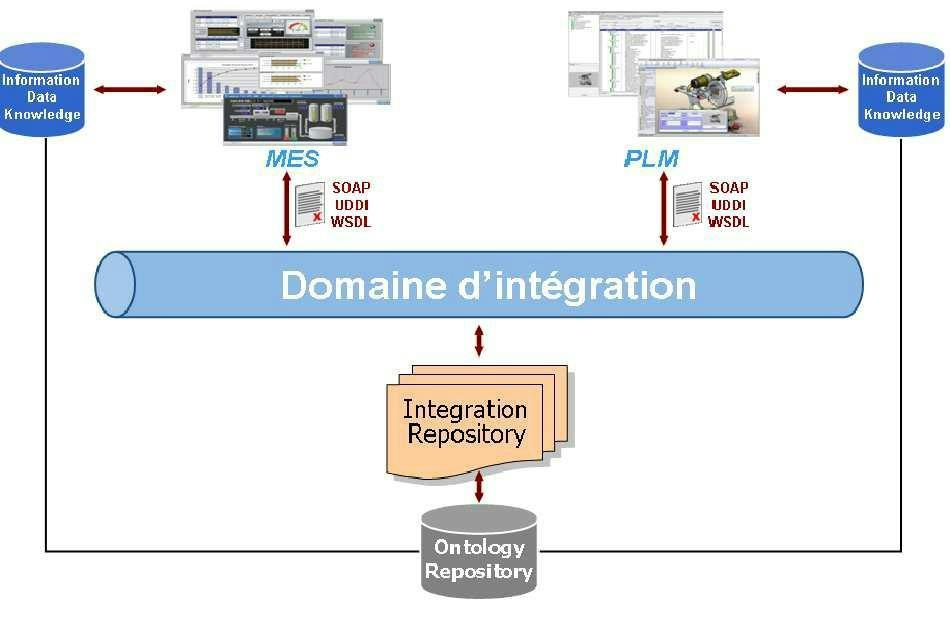
\includegraphics[width=441.67pt,height=289.45pt]{latexImage_ef9f5ece9d8f77b35dd44314351c6abe.png}}
\end{picture}
\newpage
\begin{tikzpicture}[overlay]\path(0pt,0pt);\end{tikzpicture}
\begin{picture}(-5,0)(2.5,0)
\put(500.14,-727.616){\fontsize{12}{1}\usefont{T1}{ptm}{m}{n}\selectfont\color{color_29791}14}
\put(512.14,-727.616){\fontsize{12}{1}\usefont{T1}{ptm}{m}{n}\selectfont\color{color_29791} }
\put(515.14,-727.616){\fontsize{12}{1}\usefont{T1}{ptm}{m}{n}\selectfont\color{color_29791} }
\put(70.104,-742.496){\fontsize{10.56}{1}\usefont{T1}{ptm}{m}{n}\selectfont\color{color_29791} }
\put(72.744,-742.496){\fontsize{12}{1}\usefont{T1}{ptm}{m}{n}\selectfont\color{color_29791} }
\put(84.264,-72.09998){\fontsize{12}{1}\usefont{T1}{ptm}{m}{n}\selectfont\color{color_29791} }
\put(87.26,-72.09998){\fontsize{12}{1}\usefont{T1}{ptm}{m}{n}\selectfont\color{color_29791} }
\put(87.38,-89.14001){\fontsize{14.04}{1}\usefont{T1}{ptm}{b}{n}\selectfont\color{color_29791}3}
\put(94.44212,-89.14001){\fontsize{14.04}{1}\usefont{T1}{ptm}{b}{n}\selectfont\color{color_29791}.1. }
\put(111.86,-89.14001){\fontsize{14.04}{1}\usefont{T1}{ptm}{m}{n}\selectfont\color{color_29791}這種集成在實踐}
\put(210.0136,-89.14001){\fontsize{14.04}{1}\usefont{T1}{ptm}{m}{n}\selectfont\color{color_29791}中會是什麼樣子}
\put(308.33,-89.14001){\fontsize{14.04}{1}\usefont{T1}{ptm}{b}{n}\selectfont\color{color_29791} }
\put(311.69,-89.14001){\fontsize{14.04}{1}\usefont{T1}{ptm}{b}{n}\selectfont\color{color_29791} }
\put(82.944,-123.7){\fontsize{12}{1}\usefont{T1}{ptm}{m}{n}\selectfont\color{color_29791}如第}
\put(106.94,-123.7){\fontsize{12}{1}\usefont{T1}{ptm}{m}{n}\selectfont\color{color_29791} }
\put(270.41,-123.7){\fontsize{12}{1}\usefont{T1}{ptm}{m}{n}\selectfont\color{color_29791}2 }
\put(439.87,-123.7){\fontsize{12}{1}\usefont{T1}{ptm}{m}{n}\selectfont\color{color_29791}章所述}
\put(475.9,-123.7){\fontsize{12}{1}\usefont{T1}{ptm}{m}{n}\selectfont\color{color_29791},}
\put(487.9,-123.7){\fontsize{12}{1}\usefont{T1}{ptm}{m}{n}\selectfont\color{color_29791}P}
\put(494.728,-123.7){\fontsize{12}{1}\usefont{T1}{ptm}{m}{n}\selectfont\color{color_29791}L}
\put(501.808,-123.7){\fontsize{12}{1}\usefont{T1}{ptm}{m}{n}\selectfont\color{color_29791}M }
\put(69.384,-141.34){\fontsize{12}{1}\usefont{T1}{ptm}{m}{n}\selectfont\color{color_29791}的主要思想是管理與產品相關的所有流程中的變更}
\put(333.43,-141.34){\fontsize{12}{1}\usefont{T1}{ptm}{m}{n}\selectfont\color{color_29791},}
\put(345.43,-141.34){\fontsize{12}{1}\usefont{T1}{ptm}{m}{n}\selectfont\color{color_29791}它主要通過使用虛擬化來實現}
\put(69.384,-158.98){\fontsize{12}{1}\usefont{T1}{ptm}{m}{n}\selectfont\color{color_29791}。}
\put(81.384,-158.98){\fontsize{12}{1}\usefont{T1}{ptm}{m}{n}\selectfont\color{color_29791}這裡的虛擬化一詞表示現實世界的專案對數字空間的表示}
\put(381.43,-158.98){\fontsize{12}{1}\usefont{T1}{ptm}{m}{n}\selectfont\color{color_29791},}
\put(393.43,-158.98){\fontsize{12}{1}\usefont{T1}{ptm}{m}{n}\selectfont\color{color_29791}可以想像}
\put(441.43,-158.98){\fontsize{12}{1}\usefont{T1}{ptm}{m}{n}\selectfont\color{color_29791},}
\put(453.46,-158.98){\fontsize{12}{1}\usefont{T1}{ptm}{m}{n}\selectfont\color{color_29791}有幾}
\put(477.46,-158.98){\fontsize{12}{1}\usefont{T1}{ptm}{m}{n}\selectfont\color{color_29791}個抽}
\put(69.384,-176.5){\fontsize{12}{1}\usefont{T1}{ptm}{m}{n}\selectfont\color{color_29791}象層次可以表示真實的對象或過程}
\put(249.41,-176.5){\fontsize{12}{1}\usefont{T1}{ptm}{m}{n}\selectfont\color{color_29791}。}
\put(261.41,-176.5){\fontsize{12}{1}\usefont{T1}{ptm}{m}{n}\selectfont\color{color_29791}因此}
\put(285.41,-176.5){\fontsize{12}{1}\usefont{T1}{ptm}{m}{n}\selectfont\color{color_29791},}
\put(297.41,-176.5){\fontsize{12}{1}\usefont{T1}{ptm}{m}{n}\selectfont\color{color_29791}對於虛擬表示必須達到多深和}
\put(453.46,-176.5){\fontsize{12}{1}\usefont{T1}{ptm}{m}{n}\selectfont\color{color_29791}/}
\put(456.82,-176.5){\fontsize{12}{1}\usefont{T1}{ptm}{m}{n}\selectfont\color{color_29791}或多詳細}
\put(69.384,-194.26){\fontsize{12}{1}\usefont{T1}{ptm}{m}{n}\selectfont\color{color_29791}才能達到其目的}
\put(153.38,-194.26){\fontsize{12}{1}\usefont{T1}{ptm}{m}{n}\selectfont\color{color_29791},}
\put(165.38,-194.26){\fontsize{12}{1}\usefont{T1}{ptm}{m}{n}\selectfont\color{color_29791}關於}
\put(189.41,-194.26){\fontsize{12}{1}\usefont{T1}{ptm}{m}{n}\selectfont\color{color_29791} }
\put(192.41,-194.26){\fontsize{12}{1}\usefont{T1}{ptm}{m}{n}\selectfont\color{color_29791}P}
\put(199.238,-194.26){\fontsize{12}{1}\usefont{T1}{ptm}{m}{n}\selectfont\color{color_29791}L}
\put(206.318,-194.26){\fontsize{12}{1}\usefont{T1}{ptm}{m}{n}\selectfont\color{color_29791}M }
\put(220.01,-194.26){\fontsize{12}{1}\usefont{T1}{ptm}{m}{n}\selectfont\color{color_29791}沒有確切的共識}
\put(304.13,-194.26){\fontsize{12}{1}\usefont{T1}{ptm}{m}{n}\selectfont\color{color_29791}。}
\put(316.15,-194.26){\fontsize{12}{1}\usefont{T1}{ptm}{m}{n}\selectfont\color{color_29791}  }
\put(322.15,-194.26){\fontsize{12}{1}\usefont{T1}{ptm}{m}{n}\selectfont\color{color_29791} }
\put(84.264,-211.78){\fontsize{12}{1}\usefont{T1}{ptm}{m}{n}\selectfont\color{color_29791} }
\put(87.26,-211.78){\fontsize{12}{1}\usefont{T1}{ptm}{m}{n}\selectfont\color{color_29791} }
\put(82.944,-227.86){\fontsize{12}{1}\usefont{T1}{ptm}{m}{n}\selectfont\color{color_29791}在一個理想的世界里}
\put(190.97,-227.86){\fontsize{12}{1}\usefont{T1}{ptm}{m}{n}\selectfont\color{color_29791},}
\put(202.97,-227.86){\fontsize{12}{1}\usefont{T1}{ptm}{m}{n}\selectfont\color{color_29791}這將是最低的抽象形式}
\put(322.99,-227.86){\fontsize{12}{1}\usefont{T1}{ptm}{m}{n}\selectfont\color{color_29791},}
\put(334.99,-227.86){\fontsize{12}{1}\usefont{T1}{ptm}{m}{n}\selectfont\color{color_29791}從本質上講}
\put(394.99,-227.86){\fontsize{12}{1}\usefont{T1}{ptm}{m}{n}\selectfont\color{color_29791},}
\put(406.99,-227.86){\fontsize{12}{1}\usefont{T1}{ptm}{m}{n}\selectfont\color{color_29791}它將歸結為數位孿}
\put(69.384,-245.53){\fontsize{12}{1}\usefont{T1}{ptm}{m}{n}\selectfont\color{color_29791}生}
\put(81.384,-245.53){\fontsize{12}{1}\usefont{T1}{ptm}{m}{n}\selectfont\color{color_29791},}
\put(93.38,-245.53){\fontsize{12}{1}\usefont{T1}{ptm}{m}{n}\selectfont\color{color_29791}如第}
\put(117.38,-245.53){\fontsize{12}{1}\usefont{T1}{ptm}{m}{n}\selectfont\color{color_29791}2}
\put(123.38,-245.53){\fontsize{12}{1}\usefont{T1}{ptm}{m}{n}\selectfont\color{color_29791}章所述}
\put(159.38,-245.53){\fontsize{12}{1}\usefont{T1}{ptm}{m}{n}\selectfont\color{color_29791}。}
\put(171.38,-245.53){\fontsize{12}{1}\usefont{T1}{ptm}{m}{n}\selectfont\color{color_29791}這是生產週期各個方面的}
\put(303.41,-245.53){\fontsize{12}{1}\usefont{T1}{ptm}{m}{n}\selectfont\color{color_29791}“1}
\put(314.71,-245.53){\fontsize{12}{1}\usefont{T1}{ptm}{m}{n}\selectfont\color{color_29791}對}
\put(326.71,-245.53){\fontsize{12}{1}\usefont{T1}{ptm}{m}{n}\selectfont\color{color_29791}1}
\put(332.71,-245.53){\fontsize{12}{1}\usefont{T1}{ptm}{m}{n}\selectfont\color{color_29791}”}
\put(337.99,-245.53){\fontsize{12}{1}\usefont{T1}{ptm}{m}{n}\selectfont\color{color_29791}數位表示}
\put(385.99,-245.53){\fontsize{12}{1}\usefont{T1}{ptm}{m}{n}\selectfont\color{color_29791},}
\put(397.99,-245.53){\fontsize{12}{1}\usefont{T1}{ptm}{m}{n}\selectfont\color{color_29791}其中}
\put(422.098,-245.53){\fontsize{12}{1}\usefont{T1}{ptm}{m}{n}\selectfont\color{color_29791}涉及的每個零件}
\put(69.384,-263.17){\fontsize{12}{1}\usefont{T1}{ptm}{m}{n}\selectfont\color{color_29791}都將具有數位表示}
\put(165.38,-263.17){\fontsize{12}{1}\usefont{T1}{ptm}{m}{n}\selectfont\color{color_29791},}
\put(177.38,-263.17){\fontsize{12}{1}\usefont{T1}{ptm}{m}{n}\selectfont\color{color_29791}不僅包含物品的物理特徵}
\put(309.41,-263.17){\fontsize{12}{1}\usefont{T1}{ptm}{m}{n}\selectfont\color{color_29791},}
\put(321.43,-263.17){\fontsize{12}{1}\usefont{T1}{ptm}{m}{n}\selectfont\color{color_29791}還帶有隨時間產生的所有資訊}
\put(477.46,-263.17){\fontsize{12}{1}\usefont{T1}{ptm}{m}{n}\selectfont\color{color_29791}。}
\put(489.46,-263.17){\fontsize{12}{1}\usefont{T1}{ptm}{m}{n}\selectfont\color{color_29791}為}
\put(69.384,-280.81){\fontsize{12}{1}\usefont{T1}{ptm}{m}{n}\selectfont\color{color_29791}此}
\put(81.384,-280.81){\fontsize{12}{1}\usefont{T1}{ptm}{m}{n}\selectfont\color{color_29791},}
\put(93.38,-280.81){\fontsize{12}{1}\usefont{T1}{ptm}{m}{n}\selectfont\color{color_29791}如第}
\put(117.38,-280.81){\fontsize{12}{1}\usefont{T1}{ptm}{m}{n}\selectfont\color{color_29791}2}
\put(123.38,-280.81){\fontsize{12}{1}\usefont{T1}{ptm}{m}{n}\selectfont\color{color_29791}章所述}
\put(159.38,-280.81){\fontsize{12}{1}\usefont{T1}{ptm}{m}{n}\selectfont\color{color_29791},}
\put(171.38,-280.81){\fontsize{12}{1}\usefont{T1}{ptm}{m}{n}\selectfont\color{color_29791}MES}
\put(196.13,-280.81){\fontsize{12}{1}\usefont{T1}{ptm}{m}{n}\selectfont\color{color_29791}在獲取}
\put(232.13,-280.81){\fontsize{12}{1}\usefont{T1}{ptm}{m}{n}\selectfont\color{color_29791}DT}
\put(248.09,-280.81){\fontsize{12}{1}\usefont{T1}{ptm}{m}{n}\selectfont\color{color_29791}所需的實時資訊方面發揮著重要作用}
\put(440.11,-280.81){\fontsize{12}{1}\usefont{T1}{ptm}{m}{n}\selectfont\color{color_29791}。}
\put(452.14,-280.81){\fontsize{12}{1}\usefont{T1}{ptm}{m}{n}\selectfont\color{color_29791}  }
\put(458.14,-280.81){\fontsize{12}{1}\usefont{T1}{ptm}{m}{n}\selectfont\color{color_29791} }
\put(84.264,-298.33){\fontsize{12}{1}\usefont{T1}{ptm}{m}{n}\selectfont\color{color_29791} }
\put(87.26,-298.33){\fontsize{12}{1}\usefont{T1}{ptm}{m}{n}\selectfont\color{color_29791} }
\put(82.944,-314.29){\fontsize{12}{1}\usefont{T1}{ptm}{m}{n}\selectfont\color{color_29791} }
\put(85.94,-314.29){\fontsize{12}{1}\usefont{T1}{ptm}{m}{n}\selectfont\color{color_29791}例如}
\put(109.94,-314.29){\fontsize{12}{1}\usefont{T1}{ptm}{m}{n}\selectfont\color{color_29791},}
\put(121.94,-314.29){\fontsize{12}{1}\usefont{T1}{ptm}{m}{n}\selectfont\color{color_29791}一台數控機床將有一個用於類比的數位}
\put(325.99,-314.29){\fontsize{12}{1}\usefont{T1}{ptm}{m}{n}\selectfont\color{color_29791} }
\put(497.86,-314.29){\fontsize{12}{1}\usefont{T1}{ptm}{m}{n}\selectfont\color{color_29791}3D }
\put(69.384,-331.93){\fontsize{12}{1}\usefont{T1}{ptm}{m}{n}\selectfont\color{color_29791}模型}
\put(93.38,-331.93){\fontsize{12}{1}\usefont{T1}{ptm}{m}{n}\selectfont\color{color_29791},}
\put(105.38,-331.93){\fontsize{12}{1}\usefont{T1}{ptm}{m}{n}\selectfont\color{color_29791}以及它生產的所有部件的完}
\put(249.41,-331.93){\fontsize{12}{1}\usefont{T1}{ptm}{m}{n}\selectfont\color{color_29791}全集成清單}
\put(309.41,-331.93){\fontsize{12}{1}\usefont{T1}{ptm}{m}{n}\selectfont\color{color_29791}、}
\put(321.43,-331.93){\fontsize{12}{1}\usefont{T1}{ptm}{m}{n}\selectfont\color{color_29791}有關其當前生產水平的數據}
\put(465.46,-331.93){\fontsize{12}{1}\usefont{T1}{ptm}{m}{n}\selectfont\color{color_29791}、}
\put(477.46,-331.93){\fontsize{12}{1}\usefont{T1}{ptm}{m}{n}\selectfont\color{color_29791}其機}
\put(69.384,-349.57){\fontsize{12}{1}\usefont{T1}{ptm}{m}{n}\selectfont\color{color_29791}械部件的當前磨損}
\put(165.38,-349.57){\fontsize{12}{1}\usefont{T1}{ptm}{m}{n}\selectfont\color{color_29791}、}
\put(177.38,-349.57){\fontsize{12}{1}\usefont{T1}{ptm}{m}{n}\selectfont\color{color_29791}與之相關的所有其他機器}
\put(309.41,-349.57){\fontsize{12}{1}\usefont{T1}{ptm}{m}{n}\selectfont\color{color_29791}、}
\put(321.43,-349.57){\fontsize{12}{1}\usefont{T1}{ptm}{m}{n}\selectfont\color{color_29791}受其影響的所有更改和改進的歷史}
\put(69.384,-367.09){\fontsize{12}{1}\usefont{T1}{ptm}{m}{n}\selectfont\color{color_29791}以及許多其他方面}
\put(165.38,-367.09){\fontsize{12}{1}\usefont{T1}{ptm}{m}{n}\selectfont\color{color_29791},}
\put(177.38,-367.09){\fontsize{12}{1}\usefont{T1}{ptm}{m}{n}\selectfont\color{color_29791} }
\put(184.25,-367.09){\fontsize{12}{1}\usefont{T1}{ptm}{m}{n}\selectfont\color{color_29791}所有這些都很好地封裝在一個直觀的圖形使用者介面}
\put(460.3,-367.09){\fontsize{12}{1}\usefont{T1}{ptm}{m}{n}\selectfont\color{color_29791} }
\put(467.14,-367.09){\fontsize{12}{1}\usefont{T1}{ptm}{m}{n}\selectfont\color{color_29791}(}
\put(479.14,-367.09){\fontsize{12}{1}\usefont{T1}{ptm}{m}{n}\selectfont\color{color_29791}GU}
\put(496.528,-367.09){\fontsize{12}{1}\usefont{T1}{ptm}{m}{n}\selectfont\color{color_29791}I}
\put(500.38,-367.09){\fontsize{12}{1}\usefont{T1}{ptm}{m}{n}\selectfont\color{color_29791})}
\put(512.5,-367.09){\fontsize{12}{1}\usefont{T1}{ptm}{m}{n}\selectfont\color{color_29791} }
\put(69.384,-384.85){\fontsize{12}{1}\usefont{T1}{ptm}{m}{n}\selectfont\color{color_29791}中}
\put(81.384,-384.85){\fontsize{12}{1}\usefont{T1}{ptm}{m}{n}\selectfont\color{color_29791},}
\put(93.38,-384.85){\fontsize{12}{1}\usefont{T1}{ptm}{m}{n}\selectfont\color{color_29791}允許最大程度的交互}
\put(201.41,-384.85){\fontsize{12}{1}\usefont{T1}{ptm}{m}{n}\selectfont\color{color_29791}。}
\put(213.41,-384.85){\fontsize{12}{1}\usefont{T1}{ptm}{m}{n}\selectfont\color{color_29791} }
\put(216.41,-384.85){\fontsize{12}{1}\usefont{T1}{ptm}{m}{n}\selectfont\color{color_29791} }
\put(84.264,-402.37){\fontsize{12}{1}\usefont{T1}{ptm}{m}{n}\selectfont\color{color_29791} }
\put(87.26,-402.37){\fontsize{12}{1}\usefont{T1}{ptm}{m}{n}\selectfont\color{color_29791} }
\put(82.944,-418.35){\fontsize{12}{1}\usefont{T1}{ptm}{m}{n}\selectfont\color{color_29791}在小說之外}
\put(142.94,-418.35){\fontsize{12}{1}\usefont{T1}{ptm}{m}{n}\selectfont\color{color_29791},}
\put(154.94,-418.35){\fontsize{12}{1}\usefont{T1}{ptm}{m}{n}\selectfont\color{color_29791}我們還沒有達到這樣的虛擬化水準}
\put(334.99,-418.35){\fontsize{12}{1}\usefont{T1}{ptm}{m}{n}\selectfont\color{color_29791}。}
\put(346.99,-418.35){\fontsize{12}{1}\usefont{T1}{ptm}{m}{n}\selectfont\color{color_29791}獲取和組織資訊到如此細枝末}
\put(69.384,-435.87){\fontsize{12}{1}\usefont{T1}{ptm}{m}{n}\selectfont\color{color_29791}節的水準需要花費太多的時間和金錢}
\put(261.41,-435.87){\fontsize{12}{1}\usefont{T1}{ptm}{m}{n}\selectfont\color{color_29791},}
\put(273.41,-435.87){\fontsize{12}{1}\usefont{T1}{ptm}{m}{n}\selectfont\color{color_29791}尤其是需要手動插入的方面}
\put(417.43,-435.87){\fontsize{12}{1}\usefont{T1}{ptm}{m}{n}\selectfont\color{color_29791},}
\put(429.43,-435.87){\fontsize{12}{1}\usefont{T1}{ptm}{m}{n}\selectfont\color{color_29791}更不用說如何}
\put(69.384,-453.51){\fontsize{12}{1}\usefont{T1}{ptm}{m}{n}\selectfont\color{color_29791}整合和交互這些資訊的主觀性了}
\put(237.41,-453.51){\fontsize{12}{1}\usefont{T1}{ptm}{m}{n}\selectfont\color{color_29791}。}
\put(249.41,-453.51){\fontsize{12}{1}\usefont{T1}{ptm}{m}{n}\selectfont\color{color_29791}無論如何}
\put(297.41,-453.51){\fontsize{12}{1}\usefont{T1}{ptm}{m}{n}\selectfont\color{color_29791},}
\put(309.41,-453.51){\fontsize{12}{1}\usefont{T1}{ptm}{m}{n}\selectfont\color{color_29791}在理想情況下}
\put(381.43,-453.51){\fontsize{12}{1}\usefont{T1}{ptm}{m}{n}\selectfont\color{color_29791},}
\put(393.43,-453.51){\fontsize{12}{1}\usefont{T1}{ptm}{m}{n}\selectfont\color{color_29791}確定對這種實現最重}
\put(69.384,-471.27){\fontsize{12}{1}\usefont{T1}{ptm}{m}{n}\selectfont\color{color_29791}要的方面是有用的}
\put(165.38,-471.27){\fontsize{12}{1}\usefont{T1}{ptm}{m}{n}\selectfont\color{color_29791}。}
\put(177.38,-471.27){\fontsize{12}{1}\usefont{T1}{ptm}{m}{n}\selectfont\color{color_29791}  }
\put(183.41,-471.27){\fontsize{12}{1}\usefont{T1}{ptm}{m}{n}\selectfont\color{color_29791} }
\put(84.264,-488.79){\fontsize{12}{1}\usefont{T1}{ptm}{m}{n}\selectfont\color{color_29791} }
\put(87.26,-488.79){\fontsize{12}{1}\usefont{T1}{ptm}{m}{n}\selectfont\color{color_29791} }
\put(84.264,-504.87){\fontsize{12}{1}\usefont{T1}{ptm}{m}{n}\selectfont\color{color_29791}這些是}
\put(120.26,-504.87){\fontsize{12}{1}\usefont{T1}{ptm}{m}{n}\selectfont\color{color_29791}:}
\put(132.26,-504.87){\fontsize{12}{1}\usefont{T1}{ptm}{m}{n}\selectfont\color{color_29791} }
\put(135.26,-504.87){\fontsize{12}{1}\usefont{T1}{ptm}{m}{n}\selectfont\color{color_29791} }
\put(84.264,-522.27){\fontsize{12}{1}\usefont{T1}{ptm}{m}{n}\selectfont\color{color_29791} }
\put(87.26,-522.27){\fontsize{12}{1}\usefont{T1}{ptm}{m}{n}\selectfont\color{color_29791} }
\put(88.1,-539.19){\fontsize{12}{1}\usefont{T1}{ptm}{m}{n}\selectfont\color{color_29791}}
\put(98.78,-539.19){\fontsize{12}{1}\usefont{T1}{uarial}{m}{n}\selectfont\color{color_29791} }
\put(106.1,-539.19){\fontsize{12}{1}\usefont{T1}{ptm}{m}{n}\selectfont\color{color_29791}虛擬化手段}
\put(166.1,-539.19){\fontsize{12}{1}\usefont{T1}{ptm}{m}{n}\selectfont\color{color_29791} }
\put(506.5,-539.19){\fontsize{12}{1}\usefont{T1}{ptm}{m}{n}\selectfont\color{color_29791}–}
\put(512.5,-539.19){\fontsize{12}{1}\usefont{T1}{ptm}{m}{n}\selectfont\color{color_29791} }
\put(106.1,-556.83){\fontsize{12}{1}\usefont{T1}{ptm}{m}{n}\selectfont\color{color_29791}使用什麼樣的資訊來構建虛擬物品}
\put(286.13,-556.83){\fontsize{12}{1}\usefont{T1}{ptm}{m}{n}\selectfont\color{color_29791}。}
\put(298.13,-556.83){\fontsize{12}{1}\usefont{T1}{ptm}{m}{n}\selectfont\color{color_29791}這包括直接附加到專案的元數據和檔}
\put(490.18,-556.83){\fontsize{12}{1}\usefont{T1}{ptm}{m}{n}\selectfont\color{color_29791}。}
\put(106.1,-574.59){\fontsize{12}{1}\usefont{T1}{ptm}{m}{n}\selectfont\color{color_29791}在理想情況下}
\put(178.1,-574.59){\fontsize{12}{1}\usefont{T1}{ptm}{m}{n}\selectfont\color{color_29791},}
\put(190.13,-574.59){\fontsize{12}{1}\usefont{T1}{ptm}{m}{n}\selectfont\color{color_29791}這將包含有關該專案的所有可能資訊}
\put(382.15,-574.59){\fontsize{12}{1}\usefont{T1}{ptm}{m}{n}\selectfont\color{color_29791}。}
\put(394.15,-574.59){\fontsize{12}{1}\usefont{T1}{ptm}{m}{n}\selectfont\color{color_29791}   }
\put(403.15,-574.59){\fontsize{12}{1}\usefont{T1}{ptm}{m}{n}\selectfont\color{color_29791} }
\put(84.264,-592.02){\fontsize{12}{1}\usefont{T1}{ptm}{m}{n}\selectfont\color{color_29791} }
\put(87.26,-592.02){\fontsize{12}{1}\usefont{T1}{ptm}{m}{n}\selectfont\color{color_29791} }
\put(88.1,-609.06){\fontsize{12}{1}\usefont{T1}{ptm}{m}{n}\selectfont\color{color_29791}}
\put(98.78,-609.06){\fontsize{12}{1}\usefont{T1}{uarial}{m}{n}\selectfont\color{color_29791} }
\put(106.1,-609.06){\fontsize{12}{1}\usefont{T1}{ptm}{m}{n}\selectfont\color{color_29791}數據輸入方式}
\put(178.1,-609.06){\fontsize{12}{1}\usefont{T1}{ptm}{m}{n}\selectfont\color{color_29791} }
\put(508.54,-609.06){\fontsize{12}{1}\usefont{T1}{ptm}{m}{n}\selectfont\color{color_29791}-}
\put(512.5,-609.06){\fontsize{12}{1}\usefont{T1}{ptm}{m}{n}\selectfont\color{color_29791} }
\put(106.1,-626.58){\fontsize{12}{1}\usefont{T1}{ptm}{m}{n}\selectfont\color{color_29791}如何載入和組織此資訊}
\put(226.13,-626.58){\fontsize{12}{1}\usefont{T1}{ptm}{m}{n}\selectfont\color{color_29791}。}
\put(238.13,-626.58){\fontsize{12}{1}\usefont{T1}{ptm}{m}{n}\selectfont\color{color_29791}理想情況下}
\put(298.13,-626.58){\fontsize{12}{1}\usefont{T1}{ptm}{m}{n}\selectfont\color{color_29791},}
\put(310.13,-626.58){\fontsize{12}{1}\usefont{T1}{ptm}{m}{n}\selectfont\color{color_29791}這些資訊將儘可能自動地載入到系統}
\put(106.1,-644.22){\fontsize{12}{1}\usefont{T1}{ptm}{m}{n}\selectfont\color{color_29791}中}
\put(118.1,-644.22){\fontsize{12}{1}\usefont{T1}{ptm}{m}{n}\selectfont\color{color_29791},}
\put(130.1,-644.22){\fontsize{12}{1}\usefont{T1}{ptm}{m}{n}\selectfont\color{color_29791}無論是在品質控制期間通過}
\put(274.13,-644.22){\fontsize{12}{1}\usefont{T1}{ptm}{m}{n}\selectfont\color{color_29791}MES}
\put(298.85,-644.22){\fontsize{12}{1}\usefont{T1}{ptm}{m}{n}\selectfont\color{color_29791}還是通過使用條碼掃描器等自動輸入工}
\put(106.1,-661.98){\fontsize{12}{1}\usefont{T1}{ptm}{m}{n}\selectfont\color{color_29791}具}
\put(118.1,-661.98){\fontsize{12}{1}\usefont{T1}{ptm}{m}{n}\selectfont\color{color_29791}。}
\put(130.1,-661.98){\fontsize{12}{1}\usefont{T1}{ptm}{m}{n}\selectfont\color{color_29791} }
\put(133.1,-661.98){\fontsize{12}{1}\usefont{T1}{ptm}{m}{n}\selectfont\color{color_29791} }
\put(84.264,-679.5){\fontsize{12}{1}\usefont{T1}{ptm}{m}{n}\selectfont\color{color_29791} }
\put(87.26,-679.5){\fontsize{12}{1}\usefont{T1}{ptm}{m}{n}\selectfont\color{color_29791} }
\end{picture}
\newpage
\begin{tikzpicture}[overlay]\path(0pt,0pt);\end{tikzpicture}
\begin{picture}(-5,0)(2.5,0)
\put(500.14,-727.616){\fontsize{12}{1}\usefont{T1}{ptm}{m}{n}\selectfont\color{color_29791}15}
\put(512.14,-727.616){\fontsize{12}{1}\usefont{T1}{ptm}{m}{n}\selectfont\color{color_29791} }
\put(515.14,-727.616){\fontsize{12}{1}\usefont{T1}{ptm}{m}{n}\selectfont\color{color_29791} }
\put(70.104,-742.496){\fontsize{10.56}{1}\usefont{T1}{ptm}{m}{n}\selectfont\color{color_29791} }
\put(72.744,-742.496){\fontsize{12}{1}\usefont{T1}{ptm}{m}{n}\selectfont\color{color_29791} }
\put(88.1,-72.34003){\fontsize{12}{1}\usefont{T1}{ptm}{m}{n}\selectfont\color{color_29791}}
\put(98.78,-72.34003){\fontsize{12}{1}\usefont{T1}{uarial}{m}{n}\selectfont\color{color_29791} }
\put(106.1,-72.34003){\fontsize{12}{1}\usefont{T1}{ptm}{m}{n}\selectfont\color{color_29791}存取方式}
\put(154.1,-72.34003){\fontsize{12}{1}\usefont{T1}{ptm}{m}{n}\selectfont\color{color_29791} }
\put(506.5,-72.34003){\fontsize{12}{1}\usefont{T1}{ptm}{m}{n}\selectfont\color{color_29791}–}
\put(512.5,-72.34003){\fontsize{12}{1}\usefont{T1}{ptm}{m}{n}\selectfont\color{color_29791} }
\put(106.1,-89.97998){\fontsize{12}{1}\usefont{T1}{ptm}{m}{n}\selectfont\color{color_29791}如何向使用者呈現此資訊}
\put(238.13,-89.97998){\fontsize{12}{1}\usefont{T1}{ptm}{m}{n}\selectfont\color{color_29791}。}
\put(250.13,-89.97998){\fontsize{12}{1}\usefont{T1}{ptm}{m}{n}\selectfont\color{color_29791}儘管比前面的方面更主觀}
\put(382.15,-89.97998){\fontsize{12}{1}\usefont{T1}{ptm}{m}{n}\selectfont\color{color_29791},}
\put(394.15,-89.97998){\fontsize{12}{1}\usefont{T1}{ptm}{m}{n}\selectfont\color{color_29791}但這對於系統交互的}
\put(106.1,-107.62){\fontsize{12}{1}\usefont{T1}{ptm}{m}{n}\selectfont\color{color_29791}方式非常重要}
\put(178.1,-107.62){\fontsize{12}{1}\usefont{T1}{ptm}{m}{n}\selectfont\color{color_29791}。}
\put(190.13,-107.62){\fontsize{12}{1}\usefont{T1}{ptm}{m}{n}\selectfont\color{color_29791}信息可用性的直觀性正是}
\put(322.15,-107.62){\fontsize{12}{1}\usefont{T1}{ptm}{m}{n}\selectfont\color{color_29791} }
\put(487.9,-107.62){\fontsize{12}{1}\usefont{T1}{ptm}{m}{n}\selectfont\color{color_29791}P}
\put(494.728,-107.62){\fontsize{12}{1}\usefont{T1}{ptm}{m}{n}\selectfont\color{color_29791}L}
\put(501.808,-107.62){\fontsize{12}{1}\usefont{T1}{ptm}{m}{n}\selectfont\color{color_29791}M }
\put(106.1,-125.14){\fontsize{12}{1}\usefont{T1}{ptm}{m}{n}\selectfont\color{color_29791}的核心優勢所在}
\put(190.13,-125.14){\fontsize{12}{1}\usefont{T1}{ptm}{m}{n}\selectfont\color{color_29791}。}
\put(202.13,-125.14){\fontsize{12}{1}\usefont{T1}{ptm}{m}{n}\selectfont\color{color_29791}畢竟}
\put(226.13,-125.14){\fontsize{12}{1}\usefont{T1}{ptm}{m}{n}\selectfont\color{color_29791},}
\put(238.13,-125.14){\fontsize{12}{1}\usefont{T1}{ptm}{m}{n}\selectfont\color{color_29791}如果與系統交互的唯一方式是命令行介面}
\put(454.18,-125.14){\fontsize{12}{1}\usefont{T1}{ptm}{m}{n}\selectfont\color{color_29791},}
\put(466.18,-125.14){\fontsize{12}{1}\usefont{T1}{ptm}{m}{n}\selectfont\color{color_29791}這將使}
\put(106.1,-142.78){\fontsize{12}{1}\usefont{T1}{ptm}{m}{n}\selectfont\color{color_29791}最終使用者難以}
\put(190.13,-142.78){\fontsize{12}{1}\usefont{T1}{ptm}{m}{n}\selectfont\color{color_29791}訪問資訊}
\put(238.13,-142.78){\fontsize{12}{1}\usefont{T1}{ptm}{m}{n}\selectfont\color{color_29791},}
\put(250.13,-142.78){\fontsize{12}{1}\usefont{T1}{ptm}{m}{n}\selectfont\color{color_29791}那麼一切都將是徒勞的}
\put(370.15,-142.78){\fontsize{12}{1}\usefont{T1}{ptm}{m}{n}\selectfont\color{color_29791}(}
\put(382.15,-142.78){\fontsize{12}{1}\usefont{T1}{ptm}{m}{n}\selectfont\color{color_29791}即使其他一切都是完美}
\put(106.1,-160.54){\fontsize{12}{1}\usefont{T1}{ptm}{m}{n}\selectfont\color{color_29791}的}
\put(118.1,-160.54){\fontsize{12}{1}\usefont{T1}{ptm}{m}{n}\selectfont\color{color_29791})。}
\put(142.1,-160.54){\fontsize{12}{1}\usefont{T1}{ptm}{m}{n}\selectfont\color{color_29791}  }
\put(148.1,-160.54){\fontsize{12}{1}\usefont{T1}{ptm}{m}{n}\selectfont\color{color_29791} }
\put(84.264,-178.06){\fontsize{12}{1}\usefont{T1}{ptm}{m}{n}\selectfont\color{color_29791} }
\put(87.26,-178.06){\fontsize{12}{1}\usefont{T1}{ptm}{m}{n}\selectfont\color{color_29791} }
\put(88.1,-194.98){\fontsize{12}{1}\usefont{T1}{ptm}{m}{n}\selectfont\color{color_29791}}
\put(98.78,-194.98){\fontsize{12}{1}\usefont{T1}{uarial}{m}{n}\selectfont\color{color_29791} }
\put(106.1,-194.98){\fontsize{12}{1}\usefont{T1}{ptm}{m}{n}\selectfont\color{color_29791}集成方式}
\put(154.1,-194.98){\fontsize{12}{1}\usefont{T1}{ptm}{m}{n}\selectfont\color{color_29791} }
\put(508.54,-194.98){\fontsize{12}{1}\usefont{T1}{ptm}{m}{n}\selectfont\color{color_29791}-}
\put(512.5,-194.98){\fontsize{12}{1}\usefont{T1}{ptm}{m}{n}\selectfont\color{color_29791} }
\put(106.1,-212.62){\fontsize{12}{1}\usefont{T1}{ptm}{m}{n}\selectfont\color{color_29791}專案及其包含的資訊如何相互作用並相互受益}
\put(346.15,-212.62){\fontsize{12}{1}\usefont{T1}{ptm}{m}{n}\selectfont\color{color_29791},}
\put(358.15,-212.62){\fontsize{12}{1}\usefont{T1}{ptm}{m}{n}\selectfont\color{color_29791}即與其他系統和關鍵軟體的}
\put(106.1,-230.26){\fontsize{12}{1}\usefont{T1}{ptm}{m}{n}\selectfont\color{color_29791}集成}
\put(130.1,-230.26){\fontsize{12}{1}\usefont{T1}{ptm}{m}{n}\selectfont\color{color_29791}。}
\put(142.1,-230.26){\fontsize{12}{1}\usefont{T1}{ptm}{m}{n}\selectfont\color{color_29791}例如}
\put(166.1,-230.26){\fontsize{12}{1}\usefont{T1}{ptm}{m}{n}\selectfont\color{color_29791},}
\put(178.1,-230.26){\fontsize{12}{1}\usefont{T1}{ptm}{m}{n}\selectfont\color{color_29791}如果專案可以訪問}
\put(274.13,-230.26){\fontsize{12}{1}\usefont{T1}{ptm}{m}{n}\selectfont\color{color_29791} }
\put(495.82,-230.26){\fontsize{12}{1}\usefont{T1}{ptm}{m}{n}\selectfont\color{color_29791}c}
\put(501.1,-230.26){\fontsize{12}{1}\usefont{T1}{ptm}{m}{n}\selectfont\color{color_29791}a}
\put(506.3801,-230.26){\fontsize{12}{1}\usefont{T1}{ptm}{m}{n}\selectfont\color{color_29791}d}
\put(512.488,-230.26){\fontsize{12}{1}\usefont{T1}{ptm}{m}{n}\selectfont\color{color_29791} }
\put(106.1,-247.93){\fontsize{12}{1}\usefont{T1}{ptm}{m}{n}\selectfont\color{color_29791}檔}
\put(118.1,-247.93){\fontsize{12}{1}\usefont{T1}{ptm}{m}{n}\selectfont\color{color_29791},}
\put(130.1,-247.93){\fontsize{12}{1}\usefont{T1}{ptm}{m}{n}\selectfont\color{color_29791}則無需手動填寫元數據欄位}
\put(274.13,-247.93){\fontsize{12}{1}\usefont{T1}{ptm}{m}{n}\selectfont\color{color_29791}。}
\put(286.13,-247.93){\fontsize{12}{1}\usefont{T1}{ptm}{m}{n}\selectfont\color{color_29791}鋤頭物品可以自動影響其他物品也起到了}
\put(106.1,-265.69){\fontsize{12}{1}\usefont{T1}{ptm}{m}{n}\selectfont\color{color_29791}這方面的作用}
\put(178.1,-265.69){\fontsize{12}{1}\usefont{T1}{ptm}{m}{n}\selectfont\color{color_29791}。}
\put(190.13,-265.69){\fontsize{12}{1}\usefont{T1}{ptm}{m}{n}\selectfont\color{color_29791}    }
\put(202.13,-265.69){\fontsize{12}{1}\usefont{T1}{ptm}{m}{n}\selectfont\color{color_29791} }
\put(70.104,-283.09){\fontsize{12}{1}\usefont{T1}{ptm}{m}{n}\selectfont\color{color_29791} }
\put(73.104,-283.09){\fontsize{12}{1}\usefont{T1}{ptm}{m}{n}\selectfont\color{color_29791} }
\put(70.104,-300.37){\fontsize{12}{1}\usefont{T1}{ptm}{m}{n}\selectfont\color{color_29791} }
\put(73.104,-300.37){\fontsize{12}{1}\usefont{T1}{ptm}{m}{n}\selectfont\color{color_29791} }
\put(94.1,-300.37){\fontsize{12}{1}\usefont{T1}{ptm}{m}{n}\selectfont\color{color_29791} }
\put(97.1,-300.37){\fontsize{12}{1}\usefont{T1}{ptm}{m}{n}\selectfont\color{color_29791} }
\put(241.13,-300.37){\fontsize{12}{1}\usefont{T1}{ptm}{m}{n}\selectfont\color{color_29791} }
\end{picture}
\newpage
\begin{tikzpicture}[overlay]\path(0pt,0pt);\end{tikzpicture}
\begin{picture}(-5,0)(2.5,0)
\put(500.14,-727.616){\fontsize{12}{1}\usefont{T1}{ptm}{m}{n}\selectfont\color{color_29791}16}
\put(512.14,-727.616){\fontsize{12}{1}\usefont{T1}{ptm}{m}{n}\selectfont\color{color_29791} }
\put(515.14,-727.616){\fontsize{12}{1}\usefont{T1}{ptm}{m}{n}\selectfont\color{color_29791} }
\put(70.104,-742.496){\fontsize{10.56}{1}\usefont{T1}{ptm}{m}{n}\selectfont\color{color_29791} }
\put(72.744,-742.496){\fontsize{12}{1}\usefont{T1}{ptm}{m}{n}\selectfont\color{color_29791} }
\put(265.25,-76.17999){\fontsize{15.96}{1}\usefont{T1}{ptm}{b}{n}\selectfont\color{color_29791}4}
\put(273.2779,-76.17999){\fontsize{15.96}{1}\usefont{T1}{ptm}{b}{n}\selectfont\color{color_29791}. }
\put(281.21,-76.17999){\fontsize{15.96}{1}\usefont{T1}{ptm}{m}{n}\selectfont\color{color_29791}章節}
\put(313.39,-76.17999){\fontsize{15.96}{1}\usefont{T1}{ptm}{b}{n}\selectfont\color{color_29791}   }
\put(325.27,-76.17999){\fontsize{12}{1}\usefont{T1}{ptm}{m}{n}\selectfont\color{color_29791} }
\put(241.85,-117.82){\fontsize{15.96}{1}\usefont{T1}{ptm}{m}{n}\selectfont\color{color_29791}公}
\put(257.9217,-117.82){\fontsize{15.96}{1}\usefont{T1}{ptm}{m}{n}\selectfont\color{color_29791}司及}
\put(289.9534,-117.82){\fontsize{15.96}{1}\usefont{T1}{ptm}{m}{n}\selectfont\color{color_29791}產品}
\put(321.9851,-117.82){\fontsize{15.96}{1}\usefont{T1}{ptm}{m}{n}\selectfont\color{color_29791}介紹}
\put(354.07,-117.82){\fontsize{15.96}{1}\usefont{T1}{ptm}{b}{n}\selectfont\color{color_29791} }
\put(358.03,-117.82){\fontsize{15.96}{1}\usefont{T1}{ptm}{b}{n}\selectfont\color{color_29791} }
\put(82.944,-151.9){\fontsize{12}{1}\usefont{T1}{ptm}{m}{n}\selectfont\color{color_29791}可以想像}
\put(130.94,-151.9){\fontsize{12}{1}\usefont{T1}{ptm}{m}{n}\selectfont\color{color_29791},}
\put(142.94,-151.9){\fontsize{12}{1}\usefont{T1}{ptm}{m}{n}\selectfont\color{color_29791}這項工作的獨特之處之一是它專注於一個特定的軟體解決方案}
\put(467.02,-151.9){\fontsize{12}{1}\usefont{T1}{ptm}{m}{n}\selectfont\color{color_29791},}
\put(479.02,-151.9){\fontsize{12}{1}\usefont{T1}{ptm}{m}{n}\selectfont\color{color_29791}該解}
\put(69.384,-169.42){\fontsize{12}{1}\usefont{T1}{ptm}{m}{n}\selectfont\color{color_29791}決方案在易於實施不同類型的業務方面往往非常靈活}
\put(345.43,-169.42){\fontsize{12}{1}\usefont{T1}{ptm}{m}{n}\selectfont\color{color_29791}。}
\put(357.43,-169.42){\fontsize{12}{1}\usefont{T1}{ptm}{m}{n}\selectfont\color{color_29791}這與大多數關於}
\put(441.43,-169.42){\fontsize{12}{1}\usefont{T1}{ptm}{m}{n}\selectfont\color{color_29791}P}
\put(448.258,-169.42){\fontsize{12}{1}\usefont{T1}{ptm}{m}{n}\selectfont\color{color_29791}L}
\put(455.338,-169.42){\fontsize{12}{1}\usefont{T1}{ptm}{m}{n}\selectfont\color{color_29791}M}
\put(466.06,-169.42){\fontsize{12}{1}\usefont{T1}{ptm}{m}{n}\selectfont\color{color_29791}實施的}
\put(69.384,-187.06){\fontsize{12}{1}\usefont{T1}{ptm}{m}{n}\selectfont\color{color_29791}用例相反}
\put(117.38,-187.06){\fontsize{12}{1}\usefont{T1}{ptm}{m}{n}\selectfont\color{color_29791},}
\put(129.38,-187.06){\fontsize{12}{1}\usefont{T1}{ptm}{m}{n}\selectfont\color{color_29791}在這些用例中}
\put(201.41,-187.06){\fontsize{12}{1}\usefont{T1}{ptm}{m}{n}\selectfont\color{color_29791},}
\put(213.41,-187.06){\fontsize{12}{1}\usefont{T1}{ptm}{m}{n}\selectfont\color{color_29791}業務案例是恆定的}
\put(309.41,-187.06){\fontsize{12}{1}\usefont{T1}{ptm}{m}{n}\selectfont\color{color_29791},}
\put(321.43,-187.06){\fontsize{12}{1}\usefont{T1}{ptm}{m}{n}\selectfont\color{color_29791}系統是圍繞它構建的}
\put(429.43,-187.06){\fontsize{12}{1}\usefont{T1}{ptm}{m}{n}\selectfont\color{color_29791}。}
\put(441.43,-187.06){\fontsize{12}{1}\usefont{T1}{ptm}{m}{n}\selectfont\color{color_29791}儘管如此}
\put(489.46,-187.06){\fontsize{12}{1}\usefont{T1}{ptm}{m}{n}\selectfont\color{color_29791},}
\put(69.384,-204.7){\fontsize{12}{1}\usefont{T1}{ptm}{m}{n}\selectfont\color{color_29791}為了評估}
\put(117.38,-204.7){\fontsize{12}{1}\usefont{T1}{ptm}{m}{n}\selectfont\color{color_29791}Odoo}
\put(144.02,-204.7){\fontsize{12}{1}\usefont{T1}{ptm}{m}{n}\selectfont\color{color_29791}作為}
\put(168.02,-204.7){\fontsize{12}{1}\usefont{T1}{ptm}{m}{n}\selectfont\color{color_29791}P}
\put(174.848,-204.7){\fontsize{12}{1}\usefont{T1}{ptm}{m}{n}\selectfont\color{color_29791}L}
\put(182.048,-204.7){\fontsize{12}{1}\usefont{T1}{ptm}{m}{n}\selectfont\color{color_29791}M }
\put(505.724,-204.7){\fontsize{12}{1}\usefont{T1}{ptm}{m}{n}\selectfont\color{color_29791}+}
\put(512.444,-204.7){\fontsize{12}{1}\usefont{T1}{ptm}{m}{n}\selectfont\color{color_29791} }
\put(69.384,-222.34){\fontsize{12}{1}\usefont{T1}{ptm}{m}{n}\selectfont\color{color_29791}MES}
\put(94.1,-222.34){\fontsize{12}{1}\usefont{T1}{ptm}{m}{n}\selectfont\color{color_29791}工具}
\put(118.1,-222.34){\fontsize{12}{1}\usefont{T1}{ptm}{m}{n}\selectfont\color{color_29791},}
\put(130.1,-222.34){\fontsize{12}{1}\usefont{T1}{ptm}{m}{n}\selectfont\color{color_29791}重要的是要考慮一個例子}
\put(262.13,-222.34){\fontsize{12}{1}\usefont{T1}{ptm}{m}{n}\selectfont\color{color_29791}。}
\put(274.13,-222.34){\fontsize{12}{1}\usefont{T1}{ptm}{m}{n}\selectfont\color{color_29791}這樣做的好處是}
\put(358.15,-222.34){\fontsize{12}{1}\usefont{T1}{ptm}{m}{n}\selectfont\color{color_29791},}
\put(370.15,-222.34){\fontsize{12}{1}\usefont{T1}{ptm}{m}{n}\selectfont\color{color_29791}可以為此選擇一家虛構的}
\put(69.384,-240.1){\fontsize{12}{1}\usefont{T1}{ptm}{m}{n}\selectfont\color{color_29791}公司}
\put(93.38,-240.1){\fontsize{12}{1}\usefont{T1}{ptm}{m}{n}\selectfont\color{color_29791},}
\put(105.38,-240.1){\fontsize{12}{1}\usefont{T1}{ptm}{m}{n}\selectfont\color{color_29791}從而最大限度地提高軟體在模擬過程中的感知效果}
\put(369.43,-240.1){\fontsize{12}{1}\usefont{T1}{ptm}{m}{n}\selectfont\color{color_29791}。}
\put(381.43,-240.1){\fontsize{12}{1}\usefont{T1}{ptm}{m}{n}\selectfont\color{color_29791} }
\put(384.43,-240.1){\fontsize{12}{1}\usefont{T1}{ptm}{m}{n}\selectfont\color{color_29791} }
\put(84.264,-257.53){\fontsize{12}{1}\usefont{T1}{ptm}{m}{n}\selectfont\color{color_274846} }
\put(87.26,-257.53){\fontsize{12}{1}\usefont{T1}{ptm}{m}{n}\selectfont\color{color_29791} }
\put(82.944,-273.49){\fontsize{12}{1}\usefont{T1}{ptm}{m}{n}\selectfont\color{color_29791}它正在考慮前面提到的所有系統}
\put(250.97,-273.49){\fontsize{12}{1}\usefont{T1}{ptm}{m}{n}\selectfont\color{color_29791},}
\put(262.97,-273.49){\fontsize{12}{1}\usefont{T1}{ptm}{m}{n}\selectfont\color{color_29791}為了舉例說明}
\put(334.99,-273.49){\fontsize{12}{1}\usefont{T1}{ptm}{m}{n}\selectfont\color{color_29791},}
\put(346.99,-273.49){\fontsize{12}{1}\usefont{T1}{ptm}{m}{n}\selectfont\color{color_29791}理論公司是按照工業}
\put(455.02,-273.49){\fontsize{12}{1}\usefont{T1}{ptm}{m}{n}\selectfont\color{color_29791} }
\put(497.5,-273.49){\fontsize{12}{1}\usefont{T1}{ptm}{m}{n}\selectfont\color{color_29791}4.0 }
\put(69.384,-291.13){\fontsize{12}{1}\usefont{T1}{ptm}{m}{n}\selectfont\color{color_29791}的模式組織的}
\put(141.38,-291.13){\fontsize{12}{1}\usefont{T1}{ptm}{m}{n}\selectfont\color{color_29791}。}
\put(153.38,-291.13){\fontsize{12}{1}\usefont{T1}{ptm}{m}{n}\selectfont\color{color_29791}該公司是一家最近成立的小型外殼製造公司}
\put(381.43,-291.13){\fontsize{12}{1}\usefont{T1}{ptm}{m}{n}\selectfont\color{color_29791},}
\put(393.43,-291.13){\fontsize{12}{1}\usefont{T1}{ptm}{m}{n}\selectfont\color{color_29791}使用}
\put(417.43,-291.13){\fontsize{12}{1}\usefont{T1}{ptm}{m}{n}\selectfont\color{color_29791}塑膠注射成型作}
\put(69.384,-308.77){\fontsize{12}{1}\usefont{T1}{ptm}{m}{n}\selectfont\color{color_29791}為其主要生產手段}
\put(165.38,-308.77){\fontsize{12}{1}\usefont{T1}{ptm}{m}{n}\selectfont\color{color_29791},}
\put(177.38,-308.77){\fontsize{12}{1}\usefont{T1}{ptm}{m}{n}\selectfont\color{color_29791}並使用增材製造和快速原型製作作為其業務戰略的一部分}
\put(477.46,-308.77){\fontsize{12}{1}\usefont{T1}{ptm}{m}{n}\selectfont\color{color_29791}。}
\put(489.46,-308.77){\fontsize{12}{1}\usefont{T1}{ptm}{m}{n}\selectfont\color{color_29791}正}
\put(69.384,-326.41){\fontsize{12}{1}\usefont{T1}{ptm}{m}{n}\selectfont\color{color_29791}如第}
\put(93.38,-326.41){\fontsize{12}{1}\usefont{T1}{ptm}{m}{n}\selectfont\color{color_29791}2}
\put(99.38,-326.41){\fontsize{12}{1}\usefont{T1}{ptm}{m}{n}\selectfont\color{color_29791}章所解釋的}
\put(159.38,-326.41){\fontsize{12}{1}\usefont{T1}{ptm}{m}{n}\selectfont\color{color_29791},}
\put(171.38,-326.41){\fontsize{12}{1}\usefont{T1}{ptm}{m}{n}\selectfont\color{color_29791}這些都是工業界在創新方面所採取的路徑的一個很好的例子}
\put(483.46,-326.41){\fontsize{12}{1}\usefont{T1}{ptm}{m}{n}\selectfont\color{color_29791},}
\put(495.46,-326.41){\fontsize{12}{1}\usefont{T1}{ptm}{m}{n}\selectfont\color{color_29791}在}
\put(69.384,-344.17){\fontsize{12}{1}\usefont{T1}{ptm}{m}{n}\selectfont\color{color_29791}這種道路上}
\put(129.38,-344.17){\fontsize{12}{1}\usefont{T1}{ptm}{m}{n}\selectfont\color{color_29791},}
\put(141.38,-344.17){\fontsize{12}{1}\usefont{T1}{ptm}{m}{n}\selectfont\color{color_29791}大規模生產正變得越來越不如產品種類和上市時間重要}
\put(429.43,-344.17){\fontsize{12}{1}\usefont{T1}{ptm}{m}{n}\selectfont\color{color_29791}。}
\put(441.43,-344.17){\fontsize{12}{1}\usefont{T1}{ptm}{m}{n}\selectfont\color{color_29791}  }
\put(447.46,-344.17){\fontsize{12}{1}\usefont{T1}{ptm}{m}{n}\selectfont\color{color_29791} }
\put(84.264,-361.57){\fontsize{12}{1}\usefont{T1}{ptm}{m}{n}\selectfont\color{color_29791} }
\put(87.26,-361.57){\fontsize{12}{1}\usefont{T1}{ptm}{m}{n}\selectfont\color{color_29791} }
\put(82.944,-377.53){\fontsize{12}{1}\usefont{T1}{ptm}{m}{n}\selectfont\color{color_29791}為了最大限度地跟蹤變化}
\put(214.97,-377.53){\fontsize{12}{1}\usefont{T1}{ptm}{m}{n}\selectfont\color{color_29791},}
\put(226.97,-377.53){\fontsize{12}{1}\usefont{T1}{ptm}{m}{n}\selectfont\color{color_29791}其大部分業務都基於主要自動化機器的較低生產批次}
\put(69.384,-395.17){\fontsize{12}{1}\usefont{T1}{ptm}{m}{n}\selectfont\color{color_29791}。}
\put(81.384,-395.17){\fontsize{12}{1}\usefont{T1}{ptm}{m}{n}\selectfont\color{color_29791}該公司專注於注塑塑膠產品的生產}
\put(261.41,-395.17){\fontsize{12}{1}\usefont{T1}{ptm}{m}{n}\selectfont\color{color_29791},}
\put(273.41,-395.17){\fontsize{12}{1}\usefont{T1}{ptm}{m}{n}\selectfont\color{color_29791}並嚴重依賴柔性機械進行設置生產和原型製}
\put(69.384,-412.81){\fontsize{12}{1}\usefont{T1}{ptm}{m}{n}\selectfont\color{color_29791}作}
\put(81.384,-412.81){\fontsize{12}{1}\usefont{T1}{ptm}{m}{n}\selectfont\color{color_29791}。}
\put(93.38,-412.81){\fontsize{12}{1}\usefont{T1}{ptm}{m}{n}\selectfont\color{color_29791}考慮到這一點}
\put(165.38,-412.81){\fontsize{12}{1}\usefont{T1}{ptm}{m}{n}\selectfont\color{color_29791},}
\put(177.38,-412.81){\fontsize{12}{1}\usefont{T1}{ptm}{m}{n}\selectfont\color{color_29791}它應該足夠簡單}
\put(261.41,-412.81){\fontsize{12}{1}\usefont{T1}{ptm}{m}{n}\selectfont\color{color_29791},}
\put(273.41,-412.81){\fontsize{12}{1}\usefont{T1}{ptm}{m}{n}\selectfont\color{color_29791}可以在評估軟體的範圍內模擬產品和流程的}
\put(69.384,-430.47){\fontsize{12}{1}\usefont{T1}{ptm}{m}{n}\selectfont\color{color_29791}持續改進}
\put(117.38,-430.47){\fontsize{12}{1}\usefont{T1}{ptm}{m}{n}\selectfont\color{color_29791}。}
\put(129.38,-430.47){\fontsize{12}{1}\usefont{T1}{ptm}{m}{n}\selectfont\color{color_29791}由於這種不斷變化的生產極度依賴各種資訊管理}
\put(381.43,-430.47){\fontsize{12}{1}\usefont{T1}{ptm}{m}{n}\selectfont\color{color_29791},}
\put(393.43,-430.47){\fontsize{12}{1}\usefont{T1}{ptm}{m}{n}\selectfont\color{color_29791}因此它必須被}
\put(465.46,-430.47){\fontsize{12}{1}\usefont{T1}{ptm}{m}{n}\selectfont\color{color_29791}證明是}
\put(69.384,-448.23){\fontsize{12}{1}\usefont{T1}{ptm}{m}{n}\selectfont\color{color_29791}應用}
\put(93.38,-448.23){\fontsize{12}{1}\usefont{T1}{ptm}{m}{n}\selectfont\color{color_29791}P}
\put(100.208,-448.23){\fontsize{12}{1}\usefont{T1}{ptm}{m}{n}\selectfont\color{color_29791}L}
\put(107.288,-448.23){\fontsize{12}{1}\usefont{T1}{ptm}{m}{n}\selectfont\color{color_29791}M+}
\put(124.688,-448.23){\fontsize{12}{1}\usefont{T1}{ptm}{m}{n}\selectfont\color{color_29791}MES}
\put(149.42,-448.23){\fontsize{12}{1}\usefont{T1}{ptm}{m}{n}\selectfont\color{color_29791}的完美}
\put(185.528,-448.23){\fontsize{12}{1}\usefont{T1}{ptm}{m}{n}\selectfont\color{color_29791}基礎}
\put(209.57,-448.23){\fontsize{12}{1}\usefont{T1}{ptm}{m}{n}\selectfont\color{color_29791}。}
\put(221.57,-448.23){\fontsize{12}{1}\usefont{T1}{ptm}{m}{n}\selectfont\color{color_29791}  }
\put(227.57,-448.23){\fontsize{12}{1}\usefont{T1}{ptm}{m}{n}\selectfont\color{color_29791} }
\put(84.264,-465.63){\fontsize{12}{1}\usefont{T1}{ptm}{m}{n}\selectfont\color{color_29791} }
\put(87.26,-465.63){\fontsize{12}{1}\usefont{T1}{ptm}{m}{n}\selectfont\color{color_29791} }
\put(82.944,-481.59){\fontsize{12}{1}\usefont{T1}{ptm}{m}{n}\selectfont\color{color_29791}在這個例子中}
\put(154.94,-481.59){\fontsize{12}{1}\usefont{T1}{ptm}{m}{n}\selectfont\color{color_29791},}
\put(166.94,-481.59){\fontsize{12}{1}\usefont{T1}{ptm}{m}{n}\selectfont\color{color_29791}該公司自最近成立以來已經實施了}
\put(346.99,-481.59){\fontsize{12}{1}\usefont{T1}{ptm}{m}{n}\selectfont\color{color_29791}Odoo}
\put(373.63,-481.59){\fontsize{12}{1}\usefont{T1}{ptm}{m}{n}\selectfont\color{color_29791}軟體}
\put(397.63,-481.59){\fontsize{12}{1}\usefont{T1}{ptm}{m}{n}\selectfont\color{color_29791},}
\put(409.63,-481.59){\fontsize{12}{1}\usefont{T1}{ptm}{m}{n}\selectfont\color{color_29791}並採取了所有必要}
\put(69.384,-499.23){\fontsize{12}{1}\usefont{T1}{ptm}{m}{n}\selectfont\color{color_29791}的培訓和步驟來正確使用它}
\put(213.41,-499.23){\fontsize{12}{1}\usefont{T1}{ptm}{m}{n}\selectfont\color{color_29791}。}
\put(225.41,-499.23){\fontsize{12}{1}\usefont{T1}{ptm}{m}{n}\selectfont\color{color_29791}這樣可以消除在現有業務中實施}
\put(393.43,-499.23){\fontsize{12}{1}\usefont{T1}{ptm}{m}{n}\selectfont\color{color_29791}P}
\put(400.258,-499.23){\fontsize{12}{1}\usefont{T1}{ptm}{m}{n}\selectfont\color{color_29791}L}
\put(407.338,-499.23){\fontsize{12}{1}\usefont{T1}{ptm}{m}{n}\selectfont\color{color_29791}M+}
\put(424.846,-499.23){\fontsize{12}{1}\usefont{T1}{ptm}{m}{n}\selectfont\color{color_29791}MES}
\put(449.62,-499.23){\fontsize{12}{1}\usefont{T1}{ptm}{m}{n}\selectfont\color{color_29791}系統時常見}
\put(69.384,-516.87){\fontsize{12}{1}\usefont{T1}{ptm}{m}{n}\selectfont\color{color_29791}的界限和限制}
\put(141.38,-516.87){\fontsize{12}{1}\usefont{T1}{ptm}{m}{n}\selectfont\color{color_29791},}
\put(153.38,-516.87){\fontsize{12}{1}\usefont{T1}{ptm}{m}{n}\selectfont\color{color_29791}即對遺留系統的依賴}
\put(261.41,-516.87){\fontsize{12}{1}\usefont{T1}{ptm}{m}{n}\selectfont\color{color_29791},}
\put(273.41,-516.87){\fontsize{12}{1}\usefont{T1}{ptm}{m}{n}\selectfont\color{color_29791}對更改或與舊程式集成的管理阻力}
\put(453.46,-516.87){\fontsize{12}{1}\usefont{T1}{ptm}{m}{n}\selectfont\color{color_29791}。}
\put(465.46,-516.87){\fontsize{12}{1}\usefont{T1}{ptm}{m}{n}\selectfont\color{color_29791}這些顯}
\put(69.384,-534.51){\fontsize{12}{1}\usefont{T1}{ptm}{m}{n}\selectfont\color{color_29791}然很重要}
\put(117.38,-534.51){\fontsize{12}{1}\usefont{T1}{ptm}{m}{n}\selectfont\color{color_29791},}
\put(129.38,-534.51){\fontsize{12}{1}\usefont{T1}{ptm}{m}{n}\selectfont\color{color_29791}但不在這項工作的範圍內}
\put(261.41,-534.51){\fontsize{12}{1}\usefont{T1}{ptm}{m}{n}\selectfont\color{color_29791}。}
\put(273.41,-534.51){\fontsize{12}{1}\usefont{T1}{ptm}{m}{n}\selectfont\color{color_29791}   }
\put(282.41,-534.51){\fontsize{12}{1}\usefont{T1}{ptm}{m}{n}\selectfont\color{color_29791} }
\put(70.104,-552.03){\fontsize{12}{1}\usefont{T1}{ptm}{m}{n}\selectfont\color{color_29791} }
\put(73.104,-552.03){\fontsize{12}{1}\usefont{T1}{ptm}{m}{n}\selectfont\color{color_29791} }
\put(82.944,-567.99){\fontsize{12}{1}\usefont{T1}{ptm}{m}{n}\selectfont\color{color_29791}該公司的目標是在今年年底前生產出一款全新的產品}
\put(358.99,-567.99){\fontsize{12}{1}\usefont{T1}{ptm}{m}{n}\selectfont\color{color_29791}。}
\put(370.99,-567.99){\fontsize{12}{1}\usefont{T1}{ptm}{m}{n}\selectfont\color{color_29791}這樣做之後}
\put(430.99,-567.99){\fontsize{12}{1}\usefont{T1}{ptm}{m}{n}\selectfont\color{color_29791},}
\put(442.99,-567.99){\fontsize{12}{1}\usefont{T1}{ptm}{m}{n}\selectfont\color{color_29791}該公司改進}
\put(69.384,-585.75){\fontsize{12}{1}\usefont{T1}{ptm}{m}{n}\selectfont\color{color_29791}了該產品的生產過程}
\put(177.38,-585.75){\fontsize{12}{1}\usefont{T1}{ptm}{m}{n}\selectfont\color{color_29791}。}
\put(189.41,-585.75){\fontsize{12}{1}\usefont{T1}{ptm}{m}{n}\selectfont\color{color_29791}一旦需要改進產品}
\put(285.41,-585.75){\fontsize{12}{1}\usefont{T1}{ptm}{m}{n}\selectfont\color{color_29791},}
\put(297.41,-585.75){\fontsize{12}{1}\usefont{T1}{ptm}{m}{n}\selectfont\color{color_29791}也會進行上述改進}
\put(393.43,-585.75){\fontsize{12}{1}\usefont{T1}{ptm}{m}{n}\selectfont\color{color_29791}。}
\put(405.43,-585.75){\fontsize{12}{1}\usefont{T1}{ptm}{m}{n}\selectfont\color{color_29791} }
\put(408.43,-585.75){\fontsize{12}{1}\usefont{T1}{ptm}{m}{n}\selectfont\color{color_29791} }
\put(84.264,-603.18){\fontsize{12}{1}\usefont{T1}{ptm}{m}{n}\selectfont\color{color_29791} }
\put(87.26,-603.18){\fontsize{12}{1}\usefont{T1}{ptm}{m}{n}\selectfont\color{color_29791} }
\put(82.944,-618.42){\fontsize{12}{1}\usefont{T1}{ptm}{m}{n}\selectfont\color{color_29791}下圖}
\put(106.94,-618.42){\fontsize{12}{1}\usefont{T1}{ptm}{m}{n}\selectfont\color{color_29791}(}
\put(118.94,-618.42){\fontsize{12}{1}\usefont{T1}{ptm}{m}{n}\selectfont\color{color_29791}圖}
\put(130.94,-618.42){\fontsize{12}{1}\usefont{T1}{ptm}{m}{n}\selectfont\color{color_29791} }
\put(133.94,-618.42){\fontsize{12}{1}\usefont{T1}{ptm}{m}{n}\selectfont\color{color_29791}9}
\put(139.94,-618.42){\fontsize{12}{1}\usefont{T1}{ptm}{m}{n}\selectfont\color{color_29791})}
\put(151.94,-618.42){\fontsize{12}{1}\usefont{T1}{ptm}{m}{n}\selectfont\color{color_29791}將被視為產品開發和改進的路徑}
\put(319.99,-618.42){\fontsize{12}{1}\usefont{T1}{ptm}{m}{n}\selectfont\color{color_29791}:}
\put(331.99,-618.42){\fontsize{12}{1}\usefont{T1}{ptm}{m}{n}\selectfont\color{color_29791} }
\put(334.99,-618.42){\fontsize{12}{1}\usefont{T1}{ptm}{m}{n}\selectfont\color{color_29791} }
\end{picture}
\newpage
\begin{tikzpicture}[overlay]\path(0pt,0pt);\end{tikzpicture}
\begin{picture}(-5,0)(2.5,0)
\put(500.14,-727.616){\fontsize{12}{1}\usefont{T1}{ptm}{m}{n}\selectfont\color{color_29791}17}
\put(512.14,-727.616){\fontsize{12}{1}\usefont{T1}{ptm}{m}{n}\selectfont\color{color_29791} }
\put(515.14,-727.616){\fontsize{12}{1}\usefont{T1}{ptm}{m}{n}\selectfont\color{color_29791} }
\put(70.104,-742.496){\fontsize{10.56}{1}\usefont{T1}{ptm}{m}{n}\selectfont\color{color_29791} }
\put(72.744,-742.496){\fontsize{12}{1}\usefont{T1}{ptm}{m}{n}\selectfont\color{color_29791} }
\put(515.74,-279.01){\fontsize{12}{1}\usefont{T1}{ptm}{m}{n}\selectfont\color{color_29791} }
\put(518.74,-279.01){\fontsize{12}{1}\usefont{T1}{ptm}{m}{n}\selectfont\color{color_29791} }
\put(250.37,-301.81){\fontsize{12}{1}\usefont{T1}{ptm}{m}{n}\selectfont\color{color_29791}圖}
\put(262.49,-301.81){\fontsize{12}{1}\usefont{T1}{ptm}{b}{n}\selectfont\color{color_29791}9 }
\put(271.37,-301.81){\fontsize{12}{1}\usefont{T1}{ptm}{m}{n}\selectfont\color{color_29791}開}
\put(283.37,-301.81){\fontsize{12}{1}\usefont{T1}{ptm}{m}{n}\selectfont\color{color_29791}發示}
\put(307.478,-301.81){\fontsize{12}{1}\usefont{T1}{ptm}{m}{n}\selectfont\color{color_29791}意圖}
\put(331.63,-301.81){\fontsize{12}{1}\usefont{T1}{ptm}{b}{n}\selectfont\color{color_29791} }
\put(334.51,-301.81){\fontsize{12}{1}\usefont{T1}{ptm}{m}{n}\selectfont\color{color_29791} }
\put(70.104,-319.09){\fontsize{12}{1}\usefont{T1}{ptm}{m}{n}\selectfont\color{color_29791} }
\put(73.104,-319.09){\fontsize{12}{1}\usefont{T1}{ptm}{m}{n}\selectfont\color{color_29791} }
\put(82.944,-335.05){\fontsize{12}{1}\usefont{T1}{ptm}{m}{n}\selectfont\color{color_29791}這條道路旨在向讀者傳達一種反覆運算的開發和改進方法}
\put(382.99,-335.05){\fontsize{12}{1}\usefont{T1}{ptm}{m}{n}\selectfont\color{color_29791}。}
\put(394.99,-335.05){\fontsize{12}{1}\usefont{T1}{ptm}{m}{n}\selectfont\color{color_29791}這個想法之後是產品}
\put(69.384,-352.69){\fontsize{12}{1}\usefont{T1}{ptm}{m}{n}\selectfont\color{color_29791}設計}
\put(93.38,-352.69){\fontsize{12}{1}\usefont{T1}{ptm}{m}{n}\selectfont\color{color_29791},}
\put(105.38,-352.69){\fontsize{12}{1}\usefont{T1}{ptm}{m}{n}\selectfont\color{color_29791}原型設計和重新設計的迴圈生效}
\put(273.41,-352.69){\fontsize{12}{1}\usefont{T1}{ptm}{m}{n}\selectfont\color{color_29791},}
\put(285.41,-352.69){\fontsize{12}{1}\usefont{T1}{ptm}{m}{n}\selectfont\color{color_29791}直到獲得令人滿意的結果}
\put(417.43,-352.69){\fontsize{12}{1}\usefont{T1}{ptm}{m}{n}\selectfont\color{color_29791}。}
\put(429.43,-352.69){\fontsize{12}{1}\usefont{T1}{ptm}{m}{n}\selectfont\color{color_29791}然後}
\put(453.46,-352.69){\fontsize{12}{1}\usefont{T1}{ptm}{m}{n}\selectfont\color{color_29791},}
\put(465.46,-352.69){\fontsize{12}{1}\usefont{T1}{ptm}{m}{n}\selectfont\color{color_29791}在生產}
\put(69.384,-370.45){\fontsize{12}{1}\usefont{T1}{ptm}{m}{n}\selectfont\color{color_29791}過程中也會發生類似的迴圈}
\put(216.29,-370.45){\fontsize{12}{1}\usefont{T1}{ptm}{m}{n}\selectfont\color{color_29791}。}
\put(228.53,-370.45){\fontsize{12}{1}\usefont{T1}{ptm}{m}{n}\selectfont\color{color_29791}在此階段結束時}
\put(314.35,-370.45){\fontsize{12}{1}\usefont{T1}{ptm}{m}{n}\selectfont\color{color_29791},}
\put(326.71,-370.45){\fontsize{12}{1}\usefont{T1}{ptm}{m}{n}\selectfont\color{color_29791}初步開發完成}
\put(400.87,-370.45){\fontsize{12}{1}\usefont{T1}{ptm}{m}{n}\selectfont\color{color_29791},}
\put(413.23,-370.45){\fontsize{12}{1}\usefont{T1}{ptm}{m}{n}\selectfont\color{color_29791}實際生產可以開始}
\put(512.14,-370.45){\fontsize{12}{1}\usefont{T1}{ptm}{m}{n}\selectfont\color{color_29791}。}
\put(524.5,-370.45){\fontsize{12}{1}\usefont{T1}{ptm}{m}{n}\selectfont\color{color_29791}  }
\put(530.5,-370.45){\fontsize{12}{1}\usefont{T1}{ptm}{m}{n}\selectfont\color{color_29791} }
\put(84.264,-387.85){\fontsize{12}{1}\usefont{T1}{ptm}{m}{n}\selectfont\color{color_29791} }
\put(87.26,-387.85){\fontsize{12}{1}\usefont{T1}{ptm}{m}{n}\selectfont\color{color_29791} }
\put(82.944,-403.81){\fontsize{12}{1}\usefont{T1}{ptm}{m}{n}\selectfont\color{color_29791}正是在這一點上}
\put(166.94,-403.81){\fontsize{12}{1}\usefont{T1}{ptm}{m}{n}\selectfont\color{color_29791},}
\put(178.94,-403.81){\fontsize{12}{1}\usefont{T1}{ptm}{m}{n}\selectfont\color{color_29791}建立持續改進的方法很重要}
\put(322.99,-403.81){\fontsize{12}{1}\usefont{T1}{ptm}{m}{n}\selectfont\color{color_29791}。}
\put(334.99,-403.81){\fontsize{12}{1}\usefont{T1}{ptm}{m}{n}\selectfont\color{color_29791}就這家公司而言}
\put(418.99,-403.81){\fontsize{12}{1}\usefont{T1}{ptm}{m}{n}\selectfont\color{color_29791},}
\put(430.99,-403.81){\fontsize{12}{1}\usefont{T1}{ptm}{m}{n}\selectfont\color{color_29791}我們只考慮兩}
\put(69.384,-421.47){\fontsize{12}{1}\usefont{T1}{ptm}{m}{n}\selectfont\color{color_29791}種主要類型的升級路徑}
\put(189.41,-421.47){\fontsize{12}{1}\usefont{T1}{ptm}{m}{n}\selectfont\color{color_29791},}
\put(201.41,-421.47){\fontsize{12}{1}\usefont{T1}{ptm}{m}{n}\selectfont\color{color_29791}分別是產品升級和流程升級}
\put(345.43,-421.47){\fontsize{12}{1}\usefont{T1}{ptm}{m}{n}\selectfont\color{color_29791}。}
\put(357.43,-421.47){\fontsize{12}{1}\usefont{T1}{ptm}{m}{n}\selectfont\color{color_29791}   }
\put(366.43,-421.47){\fontsize{12}{1}\usefont{T1}{ptm}{m}{n}\selectfont\color{color_29791} }
\put(87.38,-455.79){\fontsize{14.04}{1}\usefont{T1}{ptm}{b}{n}\selectfont\color{color_29791}4}
\put(94.44212,-455.79){\fontsize{14.04}{1}\usefont{T1}{ptm}{b}{n}\selectfont\color{color_29791}.1. }
\put(111.86,-455.79){\fontsize{14.04}{1}\usefont{T1}{ptm}{m}{n}\selectfont\color{color_29791}產品和工藝}
\put(182.09,-455.79){\fontsize{14.04}{1}\usefont{T1}{ptm}{b}{n}\selectfont\color{color_29791} }
\put(185.45,-455.79){\fontsize{14.04}{1}\usefont{T1}{ptm}{b}{n}\selectfont\color{color_29791} }
\put(82.944,-490.23){\fontsize{12}{1}\usefont{T1}{ptm}{m}{n}\selectfont\color{color_29791}變化和效果是}
\put(154.94,-490.23){\fontsize{12}{1}\usefont{T1}{ptm}{m}{n}\selectfont\color{color_29791}P}
\put(161.768,-490.23){\fontsize{12}{1}\usefont{T1}{ptm}{m}{n}\selectfont\color{color_29791}L}
\put(168.848,-490.23){\fontsize{12}{1}\usefont{T1}{ptm}{m}{n}\selectfont\color{color_29791}M+}
\put(186.248,-490.23){\fontsize{12}{1}\usefont{T1}{ptm}{m}{n}\selectfont\color{color_29791}ME}
\put(204.356,-490.23){\fontsize{12}{1}\usefont{T1}{ptm}{m}{n}\selectfont\color{color_29791}S}
\put(211.13,-490.23){\fontsize{12}{1}\usefont{T1}{ptm}{m}{n}\selectfont\color{color_29791}實施的重點}
\put(271.13,-490.23){\fontsize{12}{1}\usefont{T1}{ptm}{m}{n}\selectfont\color{color_29791},}
\put(283.13,-490.23){\fontsize{12}{1}\usefont{T1}{ptm}{m}{n}\selectfont\color{color_29791}因此}
\put(307.13,-490.23){\fontsize{12}{1}\usefont{T1}{ptm}{m}{n}\selectfont\color{color_29791},}
\put(319.15,-490.23){\fontsize{12}{1}\usefont{T1}{ptm}{m}{n}\selectfont\color{color_29791}理想情況下}
\put(379.15,-490.23){\fontsize{12}{1}\usefont{T1}{ptm}{m}{n}\selectfont\color{color_29791},}
\put(391.15,-490.23){\fontsize{12}{1}\usefont{T1}{ptm}{m}{n}\selectfont\color{color_29791}所述變化的主題是可以}
\put(69.384,-507.87){\fontsize{12}{1}\usefont{T1}{ptm}{m}{n}\selectfont\color{color_29791}提供合理程度的設計自由度}
\put(213.41,-507.87){\fontsize{12}{1}\usefont{T1}{ptm}{m}{n}\selectfont\color{color_29791}。}
\put(225.41,-507.87){\fontsize{12}{1}\usefont{T1}{ptm}{m}{n}\selectfont\color{color_29791} }
\put(69.384,-525.51){\fontsize{12}{1}\usefont{T1}{ptm}{m}{n}\selectfont\color{color_29791}儘管即使在變化極其有限的殭化製造環境中}
\put(297.41,-525.51){\fontsize{12}{1}\usefont{T1}{ptm}{m}{n}\selectfont\color{color_29791},}
\put(309.41,-525.51){\fontsize{12}{1}\usefont{T1}{ptm}{m}{n}\selectfont\color{color_29791}實施良好的}
\put(369.43,-525.51){\fontsize{12}{1}\usefont{T1}{ptm}{m}{n}\selectfont\color{color_29791} }
\put(456.46,-525.51){\fontsize{12}{1}\usefont{T1}{ptm}{m}{n}\selectfont\color{color_29791}P}
\put(463.288,-525.51){\fontsize{12}{1}\usefont{T1}{ptm}{m}{n}\selectfont\color{color_29791}L}
\put(470.368,-525.51){\fontsize{12}{1}\usefont{T1}{ptm}{m}{n}\selectfont\color{color_29791}M+}
\put(487.876,-525.51){\fontsize{12}{1}\usefont{T1}{ptm}{m}{n}\selectfont\color{color_29791}MES}
\put(512.476,-525.51){\fontsize{12}{1}\usefont{T1}{ptm}{m}{n}\selectfont\color{color_29791} }
\put(69.384,-543.15){\fontsize{12}{1}\usefont{T1}{ptm}{m}{n}\selectfont\color{color_29791}的效果也應該很大}
\put(165.38,-543.15){\fontsize{12}{1}\usefont{T1}{ptm}{m}{n}\selectfont\color{color_29791},}
\put(177.38,-543.15){\fontsize{12}{1}\usefont{T1}{ptm}{m}{n}\selectfont\color{color_29791}但該系統將在創新蓬勃發展的企業中產生更多可感知的變化}
\put(489.46,-543.15){\fontsize{12}{1}\usefont{T1}{ptm}{m}{n}\selectfont\color{color_29791},}
\put(69.384,-560.91){\fontsize{12}{1}\usefont{T1}{ptm}{m}{n}\selectfont\color{color_29791}因為將有更多機會改進系統並獲得反饋}
\put(273.41,-560.91){\fontsize{12}{1}\usefont{T1}{ptm}{m}{n}\selectfont\color{color_29791}。}
\put(285.41,-560.91){\fontsize{12}{1}\usefont{T1}{ptm}{m}{n}\selectfont\color{color_29791}   }
\put(294.41,-560.91){\fontsize{12}{1}\usefont{T1}{ptm}{m}{n}\selectfont\color{color_29791} }
\put(84.264,-578.31){\fontsize{12}{1}\usefont{T1}{ptm}{m}{n}\selectfont\color{color_29791} }
\put(87.26,-578.31){\fontsize{12}{1}\usefont{T1}{ptm}{m}{n}\selectfont\color{color_29791} }
\put(82.944,-594.3){\fontsize{12}{1}\usefont{T1}{ptm}{m}{n}\selectfont\color{color_29791}從改進的角度來看}
\put(178.94,-594.3){\fontsize{12}{1}\usefont{T1}{ptm}{m}{n}\selectfont\color{color_29791},}
\put(190.97,-594.3){\fontsize{12}{1}\usefont{T1}{ptm}{m}{n}\selectfont\color{color_29791}如果將鈓金衝壓產生的產品}
\put(334.99,-594.3){\fontsize{12}{1}\usefont{T1}{ptm}{m}{n}\selectfont\color{color_29791}(}
\put(346.99,-594.3){\fontsize{12}{1}\usefont{T1}{ptm}{m}{n}\selectfont\color{color_29791}圖}
\put(358.99,-594.3){\fontsize{12}{1}\usefont{T1}{ptm}{m}{n}\selectfont\color{color_29791}10}
\put(370.99,-594.3){\fontsize{12}{1}\usefont{T1}{ptm}{m}{n}\selectfont\color{color_29791})}
\put(382.99,-594.3){\fontsize{12}{1}\usefont{T1}{ptm}{m}{n}\selectfont\color{color_29791}與}
\put(394.99,-594.3){\fontsize{12}{1}\usefont{T1}{ptm}{m}{n}\selectfont\color{color_29791}C}
\put(403.018,-594.3){\fontsize{12}{1}\usefont{T1}{ptm}{m}{n}\selectfont\color{color_29791}NC}
\put(419.71,-594.3){\fontsize{12}{1}\usefont{T1}{ptm}{m}{n}\selectfont\color{color_29791}銑削程式的等效}
\put(69.384,-611.94){\fontsize{12}{1}\usefont{T1}{ptm}{m}{n}\selectfont\color{color_29791}產品}
\put(93.38,-611.94){\fontsize{12}{1}\usefont{T1}{ptm}{m}{n}\selectfont\color{color_29791}(}
\put(105.38,-611.94){\fontsize{12}{1}\usefont{T1}{ptm}{m}{n}\selectfont\color{color_29791}圖}
\put(117.38,-611.94){\fontsize{12}{1}\usefont{T1}{ptm}{m}{n}\selectfont\color{color_29791}11}
\put(129.38,-611.94){\fontsize{12}{1}\usefont{T1}{ptm}{m}{n}\selectfont\color{color_29791})}
\put(141.38,-611.94){\fontsize{12}{1}\usefont{T1}{ptm}{m}{n}\selectfont\color{color_29791}進行比較}
\put(189.41,-611.94){\fontsize{12}{1}\usefont{T1}{ptm}{m}{n}\selectfont\color{color_29791},}
\put(201.41,-611.94){\fontsize{12}{1}\usefont{T1}{ptm}{m}{n}\selectfont\color{color_29791}則很容易看出}
\put(273.41,-611.94){\fontsize{12}{1}\usefont{T1}{ptm}{m}{n}\selectfont\color{color_29791}C}
\put(281.438,-611.94){\fontsize{12}{1}\usefont{T1}{ptm}{m}{n}\selectfont\color{color_29791}NC}
\put(298.13,-611.94){\fontsize{12}{1}\usefont{T1}{ptm}{m}{n}\selectfont\color{color_29791}銑削產品更歡迎升級}
\put(406.15,-611.94){\fontsize{12}{1}\usefont{T1}{ptm}{m}{n}\selectfont\color{color_29791}。}
\put(418.15,-611.94){\fontsize{12}{1}\usefont{T1}{ptm}{m}{n}\selectfont\color{color_29791}雖然衝壓成本較}
\put(69.384,-629.58){\fontsize{12}{1}\usefont{T1}{ptm}{m}{n}\selectfont\color{color_29791}低}
\put(81.384,-629.58){\fontsize{12}{1}\usefont{T1}{ptm}{m}{n}\selectfont\color{color_29791}(}
\put(93.38,-629.58){\fontsize{12}{1}\usefont{T1}{ptm}{m}{n}\selectfont\color{color_29791}相比之下}
\put(141.38,-629.58){\fontsize{12}{1}\usefont{T1}{ptm}{m}{n}\selectfont\color{color_29791}),}
\put(165.38,-629.58){\fontsize{12}{1}\usefont{T1}{ptm}{m}{n}\selectfont\color{color_29791}但它依賴於生產成本極高的重質高精度金屬染料}
\put(417.43,-629.58){\fontsize{12}{1}\usefont{T1}{ptm}{m}{n}\selectfont\color{color_29791}。}
\put(429.43,-629.58){\fontsize{12}{1}\usefont{T1}{ptm}{m}{n}\selectfont\color{color_29791}這意味著對}
\put(489.46,-629.58){\fontsize{12}{1}\usefont{T1}{ptm}{m}{n}\selectfont\color{color_29791}它}
\put(69.384,-647.34){\fontsize{12}{1}\usefont{T1}{ptm}{m}{n}\selectfont\color{color_29791}進行更改的成本要高得多}
\put(204.05,-647.34){\fontsize{12}{1}\usefont{T1}{ptm}{m}{n}\selectfont\color{color_29791},}
\put(216.29,-647.34){\fontsize{12}{1}\usefont{T1}{ptm}{m}{n}\selectfont\color{color_29791}因此}
\put(240.77,-647.34){\fontsize{12}{1}\usefont{T1}{ptm}{m}{n}\selectfont\color{color_29791},}
\put(253.01,-647.34){\fontsize{12}{1}\usefont{T1}{ptm}{m}{n}\selectfont\color{color_29791}在}
\put(265.238,-647.34){\fontsize{12}{1}\usefont{T1}{ptm}{m}{n}\selectfont\color{color_29791}跟}
\put(277.466,-647.34){\fontsize{12}{1}\usefont{T1}{ptm}{m}{n}\selectfont\color{color_29791}蹤}
\put(289.694,-647.34){\fontsize{12}{1}\usefont{T1}{ptm}{m}{n}\selectfont\color{color_29791}更}
\put(301.922,-647.34){\fontsize{12}{1}\usefont{T1}{ptm}{m}{n}\selectfont\color{color_29791}改}
\put(314.27,-647.34){\fontsize{12}{1}\usefont{T1}{ptm}{m}{n}\selectfont\color{color_29791}方}
\put(326.618,-647.34){\fontsize{12}{1}\usefont{T1}{ptm}{m}{n}\selectfont\color{color_29791}面}
\put(338.966,-647.34){\fontsize{12}{1}\usefont{T1}{ptm}{m}{n}\selectfont\color{color_29791}蓬}
\put(351.314,-647.34){\fontsize{12}{1}\usefont{T1}{ptm}{m}{n}\selectfont\color{color_29791}勃}
\put(363.662,-647.34){\fontsize{12}{1}\usefont{T1}{ptm}{m}{n}\selectfont\color{color_29791}發}
\put(376.0099,-647.34){\fontsize{12}{1}\usefont{T1}{ptm}{m}{n}\selectfont\color{color_29791}展}
\put(388.3579,-647.34){\fontsize{12}{1}\usefont{T1}{ptm}{m}{n}\selectfont\color{color_29791}的}
\put(400.7059,-647.34){\fontsize{12}{1}\usefont{T1}{ptm}{m}{n}\selectfont\color{color_29791}系}
\put(413.0539,-647.34){\fontsize{12}{1}\usefont{T1}{ptm}{m}{n}\selectfont\color{color_29791}統}
\put(425.4019,-647.34){\fontsize{12}{1}\usefont{T1}{ptm}{m}{n}\selectfont\color{color_29791}的}
\put(437.7499,-647.34){\fontsize{12}{1}\usefont{T1}{ptm}{m}{n}\selectfont\color{color_29791}影}
\put(450.0979,-647.34){\fontsize{12}{1}\usefont{T1}{ptm}{m}{n}\selectfont\color{color_29791}響}
\put(462.4459,-647.34){\fontsize{12}{1}\usefont{T1}{ptm}{m}{n}\selectfont\color{color_29791}變}
\put(474.7939,-647.34){\fontsize{12}{1}\usefont{T1}{ptm}{m}{n}\selectfont\color{color_29791}得}
\put(487.1419,-647.34){\fontsize{12}{1}\usefont{T1}{ptm}{m}{n}\selectfont\color{color_29791}有}
\put(499.4899,-647.34){\fontsize{12}{1}\usefont{T1}{ptm}{m}{n}\selectfont\color{color_29791}限}
\put(512.14,-647.34){\fontsize{12}{1}\usefont{T1}{ptm}{m}{n}\selectfont\color{color_29791}。}
\put(524.5,-647.34){\fontsize{12}{1}\usefont{T1}{ptm}{m}{n}\selectfont\color{color_29791}  }
\put(530.5,-647.34){\fontsize{12}{1}\usefont{T1}{ptm}{m}{n}\selectfont\color{color_29791} }
\put(70.104,-664.74){\fontsize{12}{1}\usefont{T1}{ptm}{m}{n}\selectfont\color{color_29791} }
\put(73.104,-664.74){\fontsize{12}{1}\usefont{T1}{ptm}{m}{n}\selectfont\color{color_29791} }
\put(73.75,-278.95){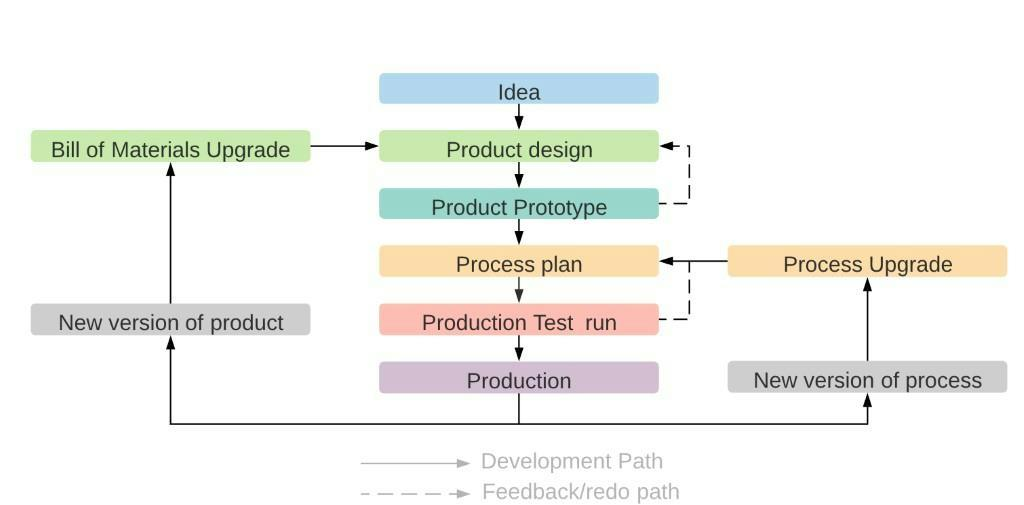
\includegraphics[width=441.9pt,height=218.05pt]{latexImage_d7c0e9b4d4314d6442b1591aaafc84fc.png}}
\end{picture}
\newpage
\begin{tikzpicture}[overlay]\path(0pt,0pt);\end{tikzpicture}
\begin{picture}(-5,0)(2.5,0)
\put(500.14,-727.616){\fontsize{12}{1}\usefont{T1}{ptm}{m}{n}\selectfont\color{color_29791}18}
\put(512.14,-727.616){\fontsize{12}{1}\usefont{T1}{ptm}{m}{n}\selectfont\color{color_29791} }
\put(515.14,-727.616){\fontsize{12}{1}\usefont{T1}{ptm}{m}{n}\selectfont\color{color_29791} }
\put(70.104,-742.496){\fontsize{10.56}{1}\usefont{T1}{ptm}{m}{n}\selectfont\color{color_29791} }
\put(72.744,-742.496){\fontsize{12}{1}\usefont{T1}{ptm}{m}{n}\selectfont\color{color_29791} }
\put(444.19,-231.94){\fontsize{12}{1}\usefont{T1}{ptm}{m}{n}\selectfont\color{color_29791} }
\put(447.22,-231.94){\fontsize{12}{1}\usefont{T1}{ptm}{m}{n}\selectfont\color{color_29791} }
\put(155.18,-244.45){\fontsize{12}{1}\usefont{T1}{ptm}{m}{n}\selectfont\color{color_29791}圖}
\put(167.3,-244.45){\fontsize{12}{1}\usefont{T1}{ptm}{b}{n}\selectfont\color{color_29791}10 }
\put(182.21,-244.45){\fontsize{12}{1}\usefont{T1}{ptm}{m}{n}\selectfont\color{color_29791}衝壓}
\put(206.33,-244.45){\fontsize{12}{1}\usefont{T1}{ptm}{b}{n}\selectfont\color{color_29791}AK}
\put(224.21,-244.45){\fontsize{12}{1}\usefont{T1}{ptm}{b}{n}\selectfont\color{color_29791}74}
\put(236.21,-244.45){\fontsize{12}{1}\usefont{T1}{ptm}{m}{n}\selectfont\color{color_29791}式}
\put(248.318,-244.45){\fontsize{12}{1}\usefont{T1}{ptm}{m}{n}\selectfont\color{color_29791}步槍機匣示例}
\put(320.47,-244.45){\fontsize{12}{1}\usefont{T1}{ptm}{m}{n}\selectfont\color{color_29791}(}
\put(332.47,-244.45){\fontsize{12}{1}\usefont{T1}{ptm}{b}{n}\selectfont\color{color_29791}B}
\put(340.498,-244.45){\fontsize{12}{1}\usefont{T1}{ptm}{b}{n}\selectfont\color{color_29791}r}
\put(345.538,-244.45){\fontsize{12}{1}\usefont{T1}{ptm}{b}{n}\selectfont\color{color_29791}ow}
\put(360.286,-244.45){\fontsize{12}{1}\usefont{T1}{ptm}{b}{n}\selectfont\color{color_29791}n}
\put(366.886,-244.45){\fontsize{12}{1}\usefont{T1}{ptm}{b}{n}\selectfont\color{color_29791}n}
\put(373.594,-244.45){\fontsize{12}{1}\usefont{T1}{ptm}{b}{n}\selectfont\color{color_29791}e}
\put(378.874,-244.45){\fontsize{12}{1}\usefont{T1}{ptm}{b}{n}\selectfont\color{color_29791}ll}
\put(385.582,-244.45){\fontsize{12}{1}\usefont{T1}{ptm}{b}{n}\selectfont\color{color_29791}s.}
\put(393.142,-244.45){\fontsize{12}{1}\usefont{T1}{ptm}{b}{n}\selectfont\color{color_29791}c}
\put(398.422,-244.45){\fontsize{12}{1}\usefont{T1}{ptm}{b}{n}\selectfont\color{color_29791}o}
\put(404.53,-244.45){\fontsize{12}{1}\usefont{T1}{ptm}{b}{n}\selectfont\color{color_29791}m}
\put(414.43,-244.45){\fontsize{12}{1}\usefont{T1}{ptm}{m}{n}\selectfont\color{color_29791})}
\put(426.55,-244.45){\fontsize{12}{1}\usefont{T1}{ptm}{b}{n}\selectfont\color{color_29791} }
\put(429.55,-244.45){\fontsize{12}{1}\usefont{T1}{ptm}{m}{n}\selectfont\color{color_29791} }
\put(444.43,-400.81){\fontsize{12}{1}\usefont{T1}{ptm}{m}{n}\selectfont\color{color_29791} }
\put(447.46,-400.81){\fontsize{12}{1}\usefont{T1}{ptm}{m}{n}\selectfont\color{color_29791} }
\put(155.9,-413.29){\fontsize{12}{1}\usefont{T1}{ptm}{m}{n}\selectfont\color{color_29791}圖}
\put(168.02,-413.29){\fontsize{12}{1}\usefont{T1}{ptm}{b}{n}\selectfont\color{color_29791}11 }
\put(182.93,-413.29){\fontsize{12}{1}\usefont{T1}{ptm}{m}{n}\selectfont\color{color_29791}銑削}
\put(207.05,-413.29){\fontsize{12}{1}\usefont{T1}{ptm}{b}{n}\selectfont\color{color_29791}AK}
\put(224.93,-413.29){\fontsize{12}{1}\usefont{T1}{ptm}{b}{n}\selectfont\color{color_29791}74}
\put(236.93,-413.29){\fontsize{12}{1}\usefont{T1}{ptm}{m}{n}\selectfont\color{color_29791}型}
\put(249.038,-413.29){\fontsize{12}{1}\usefont{T1}{ptm}{m}{n}\selectfont\color{color_29791}步槍機匣示例}
\put(321.19,-413.29){\fontsize{12}{1}\usefont{T1}{ptm}{m}{n}\selectfont\color{color_29791}(}
\put(333.19,-413.29){\fontsize{12}{1}\usefont{T1}{ptm}{b}{n}\selectfont\color{color_29791}sh}
\put(344.578,-413.29){\fontsize{12}{1}\usefont{T1}{ptm}{b}{n}\selectfont\color{color_29791}ar}
\put(355.858,-413.29){\fontsize{12}{1}\usefont{T1}{ptm}{b}{n}\selectfont\color{color_29791}p}
\put(362.566,-413.29){\fontsize{12}{1}\usefont{T1}{ptm}{b}{n}\selectfont\color{color_29791}sb}
\put(373.954,-413.29){\fontsize{12}{1}\usefont{T1}{ptm}{b}{n}\selectfont\color{color_29791}r}
\put(378.994,-413.29){\fontsize{12}{1}\usefont{T1}{ptm}{b}{n}\selectfont\color{color_29791}os.}
\put(392.554,-413.29){\fontsize{12}{1}\usefont{T1}{ptm}{b}{n}\selectfont\color{color_29791}c}
\put(397.834,-413.29){\fontsize{12}{1}\usefont{T1}{ptm}{b}{n}\selectfont\color{color_29791}o}
\put(403.942,-413.29){\fontsize{12}{1}\usefont{T1}{ptm}{b}{n}\selectfont\color{color_29791}m}
\put(413.83,-413.29){\fontsize{12}{1}\usefont{T1}{ptm}{m}{n}\selectfont\color{color_29791})}
\put(425.95,-413.29){\fontsize{12}{1}\usefont{T1}{ptm}{b}{n}\selectfont\color{color_29791} }
\put(428.95,-413.29){\fontsize{12}{1}\usefont{T1}{ptm}{m}{n}\selectfont\color{color_29791} }
\put(70.104,-430.71){\fontsize{12}{1}\usefont{T1}{ptm}{m}{n}\selectfont\color{color_29791} }
\put(73.104,-430.71){\fontsize{12}{1}\usefont{T1}{ptm}{m}{n}\selectfont\color{color_29791} }
\put(82.944,-446.55){\fontsize{12}{1}\usefont{T1}{ptm}{m}{n}\selectfont\color{color_29791}就這家虛構的公司而言}
\put(202.97,-446.55){\fontsize{12}{1}\usefont{T1}{ptm}{m}{n}\selectfont\color{color_29791},}
\put(214.97,-446.55){\fontsize{12}{1}\usefont{T1}{ptm}{m}{n}\selectfont\color{color_29791}已經確定}
\put(262.97,-446.55){\fontsize{12}{1}\usefont{T1}{ptm}{m}{n}\selectfont\color{color_29791},}
\put(274.97,-446.55){\fontsize{12}{1}\usefont{T1}{ptm}{m}{n}\selectfont\color{color_29791}體現}
\put(298.97,-446.55){\fontsize{12}{1}\usefont{T1}{ptm}{m}{n}\selectfont\color{color_29791} }
\put(456.34,-446.55){\fontsize{12}{1}\usefont{T1}{ptm}{m}{n}\selectfont\color{color_29791}P}
\put(463.168,-446.55){\fontsize{12}{1}\usefont{T1}{ptm}{m}{n}\selectfont\color{color_29791}L}
\put(470.248,-446.55){\fontsize{12}{1}\usefont{T1}{ptm}{m}{n}\selectfont\color{color_29791}M+}
\put(487.648,-446.55){\fontsize{12}{1}\usefont{T1}{ptm}{m}{n}\selectfont\color{color_29791}MES}
\put(512.476,-446.55){\fontsize{12}{1}\usefont{T1}{ptm}{m}{n}\selectfont\color{color_29791} }
\put(69.384,-464.19){\fontsize{12}{1}\usefont{T1}{ptm}{m}{n}\selectfont\color{color_29791}效應的最佳方式是圍繞塑膠注射成型設計產品}
\put(309.41,-464.19){\fontsize{12}{1}\usefont{T1}{ptm}{m}{n}\selectfont\color{color_29791}。}
\put(321.43,-464.19){\fontsize{12}{1}\usefont{T1}{ptm}{m}{n}\selectfont\color{color_29791}乍一看}
\put(357.43,-464.19){\fontsize{12}{1}\usefont{T1}{ptm}{m}{n}\selectfont\color{color_29791},}
\put(369.43,-464.19){\fontsize{12}{1}\usefont{T1}{ptm}{m}{n}\selectfont\color{color_29791}考慮這種製造程式似乎不}
\put(69.384,-481.83){\fontsize{12}{1}\usefont{T1}{ptm}{m}{n}\selectfont\color{color_29791}直觀}
\put(93.38,-481.83){\fontsize{12}{1}\usefont{T1}{ptm}{m}{n}\selectfont\color{color_29791},}
\put(105.38,-481.83){\fontsize{12}{1}\usefont{T1}{ptm}{m}{n}\selectfont\color{color_29791}就像前面描述的衝壓程式一樣}
\put(261.41,-481.83){\fontsize{12}{1}\usefont{T1}{ptm}{m}{n}\selectfont\color{color_29791},}
\put(273.41,-481.83){\fontsize{12}{1}\usefont{T1}{ptm}{m}{n}\selectfont\color{color_29791}因為它在生產過程中也依賴於高精度模具}
\put(489.46,-481.83){\fontsize{12}{1}\usefont{T1}{ptm}{m}{n}\selectfont\color{color_29791}。}
\put(69.384,-499.59){\fontsize{12}{1}\usefont{T1}{ptm}{m}{n}\selectfont\color{color_29791}然而}
\put(93.38,-499.59){\fontsize{12}{1}\usefont{T1}{ptm}{m}{n}\selectfont\color{color_29791},}
\put(105.38,-499.59){\fontsize{12}{1}\usefont{T1}{ptm}{m}{n}\selectfont\color{color_29791}兩者之間的主要區別在於原型製作的便利性和升級成本}
\put(393.43,-499.59){\fontsize{12}{1}\usefont{T1}{ptm}{m}{n}\selectfont\color{color_29791}。}
\put(405.43,-499.59){\fontsize{12}{1}\usefont{T1}{ptm}{m}{n}\selectfont\color{color_29791}  }
\put(411.43,-499.59){\fontsize{12}{1}\usefont{T1}{ptm}{m}{n}\selectfont\color{color_29791} }
\put(84.264,-517.11){\fontsize{12}{1}\usefont{T1}{ptm}{m}{n}\selectfont\color{color_29791} }
\put(87.26,-517.11){\fontsize{12}{1}\usefont{T1}{ptm}{m}{n}\selectfont\color{color_29791} }
\put(82.944,-532.95){\fontsize{12}{1}\usefont{T1}{ptm}{m}{n}\selectfont\color{color_29791}注塑成型是一個廣泛而複雜的工程領域}
\put(286.97,-532.95){\fontsize{12}{1}\usefont{T1}{ptm}{m}{n}\selectfont\color{color_29791},}
\put(298.97,-532.95){\fontsize{12}{1}\usefont{T1}{ptm}{m}{n}\selectfont\color{color_29791}涉及種類繁多的材料和方法}
\put(442.99,-532.95){\fontsize{12}{1}\usefont{T1}{ptm}{m}{n}\selectfont\color{color_29791},}
\put(455.02,-532.95){\fontsize{12}{1}\usefont{T1}{ptm}{m}{n}\selectfont\color{color_29791}其中很少}
\put(69.384,-550.59){\fontsize{12}{1}\usefont{T1}{ptm}{m}{n}\selectfont\color{color_29791}是這項工作所關注的}
\put(177.38,-550.59){\fontsize{12}{1}\usefont{T1}{ptm}{m}{n}\selectfont\color{color_29791}。}
\put(189.41,-550.59){\fontsize{12}{1}\usefont{T1}{ptm}{m}{n}\selectfont\color{color_29791}然而}
\put(213.41,-550.59){\fontsize{12}{1}\usefont{T1}{ptm}{m}{n}\selectfont\color{color_29791},}
\put(225.41,-550.59){\fontsize{12}{1}\usefont{T1}{ptm}{m}{n}\selectfont\color{color_29791}需要指出的是}
\put(297.41,-550.59){\fontsize{12}{1}\usefont{T1}{ptm}{m}{n}\selectfont\color{color_29791},}
\put(309.41,-550.59){\fontsize{12}{1}\usefont{T1}{ptm}{m}{n}\selectfont\color{color_29791}在大多數情況下}
\put(393.43,-550.59){\fontsize{12}{1}\usefont{T1}{ptm}{m}{n}\selectfont\color{color_29791},}
\put(405.43,-550.59){\fontsize{12}{1}\usefont{T1}{ptm}{m}{n}\selectfont\color{color_29791}注塑成型中涉及的}
\put(69.384,-568.23){\fontsize{12}{1}\usefont{T1}{ptm}{m}{n}\selectfont\color{color_29791}壓力比我們處理鋼時的壓力低一個數量級}
\put(285.41,-568.23){\fontsize{12}{1}\usefont{T1}{ptm}{m}{n}\selectfont\color{color_29791};}
\put(288.77,-568.23){\fontsize{12}{1}\usefont{T1}{ptm}{m}{n}\selectfont\color{color_29791}較軟的材料可用於他們的模具}
\put(444.79,-568.23){\fontsize{12}{1}\usefont{T1}{ptm}{m}{n}\selectfont\color{color_29791},}
\put(456.82,-568.23){\fontsize{12}{1}\usefont{T1}{ptm}{m}{n}\selectfont\color{color_29791}例如}
\put(480.82,-568.23){\fontsize{12}{1}\usefont{T1}{ptm}{m}{n}\selectfont\color{color_29791} }
\put(487.9,-568.23){\fontsize{12}{1}\usefont{T1}{ptm}{m}{n}\selectfont\color{color_29791}C}
\put(495.928,-568.23){\fontsize{12}{1}\usefont{T1}{ptm}{m}{n}\selectfont\color{color_29791}NC}
\put(512.488,-568.23){\fontsize{12}{1}\usefont{T1}{ptm}{m}{n}\selectfont\color{color_29791} }
\put(69.384,-585.87){\fontsize{12}{1}\usefont{T1}{ptm}{m}{n}\selectfont\color{color_29791}銑削鋁}
\put(105.38,-585.87){\fontsize{12}{1}\usefont{T1}{ptm}{m}{n}\selectfont\color{color_29791}。}
\put(117.38,-585.87){\fontsize{12}{1}\usefont{T1}{ptm}{m}{n}\selectfont\color{color_29791}同時}
\put(141.38,-585.87){\fontsize{12}{1}\usefont{T1}{ptm}{m}{n}\selectfont\color{color_29791},}
\put(153.38,-585.87){\fontsize{12}{1}\usefont{T1}{ptm}{m}{n}\selectfont\color{color_29791}增材製造領域的新進展使得塑膠部件的原型設計成為可能}
\put(453.46,-585.87){\fontsize{12}{1}\usefont{T1}{ptm}{m}{n}\selectfont\color{color_29791},}
\put(465.46,-585.87){\fontsize{12}{1}\usefont{T1}{ptm}{m}{n}\selectfont\color{color_29791}這些塑}
\put(69.384,-603.54){\fontsize{12}{1}\usefont{T1}{ptm}{m}{n}\selectfont\color{color_29791}膠部件的物理特性更接近注塑件的最終結果}
\put(297.41,-603.54){\fontsize{12}{1}\usefont{T1}{ptm}{m}{n}\selectfont\color{color_29791}。}
\put(309.41,-603.54){\fontsize{12}{1}\usefont{T1}{ptm}{m}{n}\selectfont\color{color_29791}有時}
\put(333.43,-603.54){\fontsize{12}{1}\usefont{T1}{ptm}{m}{n}\selectfont\color{color_29791},}
\put(345.43,-603.54){\fontsize{12}{1}\usefont{T1}{ptm}{m}{n}\selectfont\color{color_29791}在工藝升級期間}
\put(429.43,-603.54){\fontsize{12}{1}\usefont{T1}{ptm}{m}{n}\selectfont\color{color_29791},}
\put(441.43,-603.54){\fontsize{12}{1}\usefont{T1}{ptm}{m}{n}\selectfont\color{color_29791}甚至可以使}
\put(69.384,-621.3){\fontsize{12}{1}\usefont{T1}{ptm}{m}{n}\selectfont\color{color_29791}用原型模具}
\put(129.38,-621.3){\fontsize{12}{1}\usefont{T1}{ptm}{m}{n}\selectfont\color{color_29791}(}
\put(141.38,-621.3){\fontsize{12}{1}\usefont{T1}{ptm}{m}{n}\selectfont\color{color_29791}圖}
\put(153.38,-621.3){\fontsize{12}{1}\usefont{T1}{ptm}{m}{n}\selectfont\color{color_29791} }
\put(156.38,-621.3){\fontsize{12}{1}\usefont{T1}{ptm}{m}{n}\selectfont\color{color_29791}12}
\put(168.38,-621.3){\fontsize{12}{1}\usefont{T1}{ptm}{m}{n}\selectfont\color{color_29791})}
\put(180.41,-621.3){\fontsize{12}{1}\usefont{T1}{ptm}{m}{n}\selectfont\color{color_29791}進行小批量測試}
\put(264.41,-621.3){\fontsize{12}{1}\usefont{T1}{ptm}{m}{n}\selectfont\color{color_29791}。}
\put(276.41,-621.3){\fontsize{12}{1}\usefont{T1}{ptm}{m}{n}\selectfont\color{color_29791}  }
\put(282.41,-621.3){\fontsize{12}{1}\usefont{T1}{ptm}{m}{n}\selectfont\color{color_29791} }
\put(70.104,-638.7){\fontsize{12}{1}\usefont{T1}{ptm}{m}{n}\selectfont\color{color_29791} }
\put(73.104,-638.7){\fontsize{12}{1}\usefont{T1}{ptm}{m}{n}\selectfont\color{color_29791} }
\put(144.1,-231.9){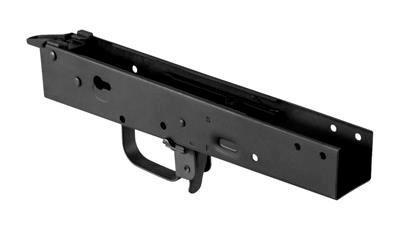
\includegraphics[width=300pt,height=171pt]{latexImage_2e6550d3563c82c814da39c1e4b27b13.png}}
\put(143.85,-400.79){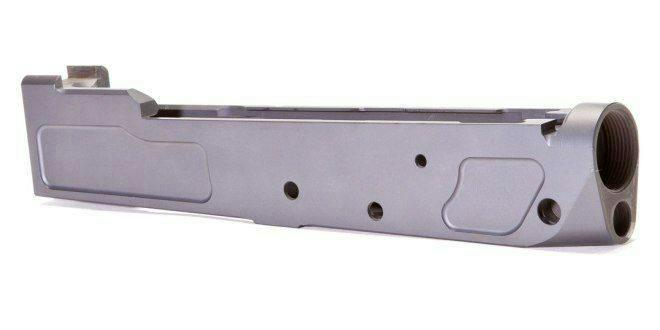
\includegraphics[width=300.5pt,height=150.25pt]{latexImage_e8147699f7eb76691552a3b9daab46cd.png}}
\end{picture}
\newpage
\begin{tikzpicture}[overlay]\path(0pt,0pt);\end{tikzpicture}
\begin{picture}(-5,0)(2.5,0)
\put(500.14,-727.616){\fontsize{12}{1}\usefont{T1}{ptm}{m}{n}\selectfont\color{color_29791}19}
\put(512.14,-727.616){\fontsize{12}{1}\usefont{T1}{ptm}{m}{n}\selectfont\color{color_29791} }
\put(515.14,-727.616){\fontsize{12}{1}\usefont{T1}{ptm}{m}{n}\selectfont\color{color_29791} }
\put(70.104,-742.496){\fontsize{10.56}{1}\usefont{T1}{ptm}{m}{n}\selectfont\color{color_29791} }
\put(72.744,-742.496){\fontsize{12}{1}\usefont{T1}{ptm}{m}{n}\selectfont\color{color_29791} }
\put(515.74,-355.57){\fontsize{12}{1}\usefont{T1}{ptm}{m}{n}\selectfont\color{color_29791} }
\put(518.74,-355.57){\fontsize{12}{1}\usefont{T1}{ptm}{m}{n}\selectfont\color{color_29791} }
\put(128.42,-368.05){\fontsize{12}{1}\usefont{T1}{ptm}{m}{n}\selectfont\color{color_29791}圖}
\put(140.54,-368.05){\fontsize{12}{1}\usefont{T1}{ptm}{b}{n}\selectfont\color{color_29791}12 }
\put(155.42,-368.05){\fontsize{12}{1}\usefont{T1}{ptm}{m}{n}\selectfont\color{color_29791}使用}
\put(179.54,-368.05){\fontsize{12}{1}\usefont{T1}{ptm}{b}{n}\selectfont\color{color_29791}3}
\put(185.57,-368.05){\fontsize{12}{1}\usefont{T1}{ptm}{b}{n}\selectfont\color{color_29791}D}
\put(194.21,-368.05){\fontsize{12}{1}\usefont{T1}{ptm}{m}{n}\selectfont\color{color_29791}列印機制作的注塑}
\put(290.318,-368.05){\fontsize{12}{1}\usefont{T1}{ptm}{m}{n}\selectfont\color{color_29791}模具示例}
\put(338.35,-368.05){\fontsize{12}{1}\usefont{T1}{ptm}{m}{n}\selectfont\color{color_29791}(}
\put(350.47,-368.05){\fontsize{12}{1}\usefont{T1}{ptm}{b}{n}\selectfont\color{color_29791}th}
\put(361.03,-368.05){\fontsize{12}{1}\usefont{T1}{ptm}{b}{n}\selectfont\color{color_29791}e}
\put(366.31,-368.05){\fontsize{12}{1}\usefont{T1}{ptm}{b}{n}\selectfont\color{color_29791}f}
\put(370.378,-368.05){\fontsize{12}{1}\usefont{T1}{ptm}{b}{n}\selectfont\color{color_29791}ab}
\put(383.086,-368.05){\fontsize{12}{1}\usefont{T1}{ptm}{b}{n}\selectfont\color{color_29791}r}
\put(388.366,-368.05){\fontsize{12}{1}\usefont{T1}{ptm}{b}{n}\selectfont\color{color_29791}icat}
\put(406.966,-368.05){\fontsize{12}{1}\usefont{T1}{ptm}{b}{n}\selectfont\color{color_29791}or}
\put(417.166,-368.05){\fontsize{12}{1}\usefont{T1}{ptm}{b}{n}\selectfont\color{color_29791}.c}
\put(425.446,-368.05){\fontsize{12}{1}\usefont{T1}{ptm}{b}{n}\selectfont\color{color_29791}o}
\put(431.554,-368.05){\fontsize{12}{1}\usefont{T1}{ptm}{b}{n}\selectfont\color{color_29791}m}
\put(441.43,-368.05){\fontsize{12}{1}\usefont{T1}{ptm}{m}{n}\selectfont\color{color_29791})}
\put(453.58,-368.05){\fontsize{12}{1}\usefont{T1}{ptm}{b}{n}\selectfont\color{color_29791} }
\put(456.58,-368.05){\fontsize{12}{1}\usefont{T1}{ptm}{m}{n}\selectfont\color{color_29791} }
\put(70.104,-385.33){\fontsize{12}{1}\usefont{T1}{ptm}{m}{n}\selectfont\color{color_29791} }
\put(73.104,-385.33){\fontsize{12}{1}\usefont{T1}{ptm}{m}{n}\selectfont\color{color_29791} }
\put(82.944,-400.45){\fontsize{12}{1}\usefont{T1}{ptm}{m}{n}\selectfont\color{color_29791}增材製}
\put(118.94,-400.45){\fontsize{12}{1}\usefont{T1}{ptm}{m}{n}\selectfont\color{color_29791}造已成為超柔性生產的絕佳工具}
\put(286.97,-400.45){\fontsize{12}{1}\usefont{T1}{ptm}{m}{n}\selectfont\color{color_29791}。}
\put(298.97,-400.45){\fontsize{12}{1}\usefont{T1}{ptm}{m}{n}\selectfont\color{color_29791}這種持續改進的心態}
\put(406.99,-400.45){\fontsize{12}{1}\usefont{T1}{ptm}{m}{n}\selectfont\color{color_29791},}
\put(418.99,-400.45){\fontsize{12}{1}\usefont{T1}{ptm}{m}{n}\selectfont\color{color_29791}尤其是在原型設}
\put(69.384,-418.23){\fontsize{12}{1}\usefont{T1}{ptm}{m}{n}\selectfont\color{color_29791}計和反覆運算設計方面}
\put(189.41,-418.23){\fontsize{12}{1}\usefont{T1}{ptm}{m}{n}\selectfont\color{color_29791},}
\put(201.41,-418.23){\fontsize{12}{1}\usefont{T1}{ptm}{m}{n}\selectfont\color{color_29791}是精益心態的標誌}
\put(297.41,-418.23){\fontsize{12}{1}\usefont{T1}{ptm}{m}{n}\selectfont\color{color_29791},}
\put(309.41,-418.23){\fontsize{12}{1}\usefont{T1}{ptm}{m}{n}\selectfont\color{color_29791}這種心態在現代工業中是如此重要}
\put(489.46,-418.23){\fontsize{12}{1}\usefont{T1}{ptm}{m}{n}\selectfont\color{color_29791}。}
\put(501.46,-418.23){\fontsize{12}{1}\usefont{T1}{ptm}{m}{n}\selectfont\color{color_29791}  }
\put(507.46,-418.23){\fontsize{12}{1}\usefont{T1}{ptm}{m}{n}\selectfont\color{color_29791} }
\put(84.264,-435.75){\fontsize{12}{1}\usefont{T1}{ptm}{m}{n}\selectfont\color{color_29791} }
\put(87.26,-435.75){\fontsize{12}{1}\usefont{T1}{ptm}{m}{n}\selectfont\color{color_29791} }
\put(82.944,-451.59){\fontsize{12}{1}\usefont{T1}{ptm}{m}{n}\selectfont\color{color_29791}如上一節所述}
\put(154.94,-451.59){\fontsize{12}{1}\usefont{T1}{ptm}{m}{n}\selectfont\color{color_29791},}
\put(166.94,-451.59){\fontsize{12}{1}\usefont{T1}{ptm}{m}{n}\selectfont\color{color_29791}在本案例研究中}
\put(250.97,-451.59){\fontsize{12}{1}\usefont{T1}{ptm}{m}{n}\selectfont\color{color_29791},}
\put(262.97,-451.59){\fontsize{12}{1}\usefont{T1}{ptm}{m}{n}\selectfont\color{color_29791}它被認為是虛構公司創造新產品及其生產過程}
\put(69.384,-469.23){\fontsize{12}{1}\usefont{T1}{ptm}{m}{n}\selectfont\color{color_29791}。}
\put(81.384,-469.23){\fontsize{12}{1}\usefont{T1}{ptm}{m}{n}\selectfont\color{color_29791}該產品由一個塑膠小型計算機機箱組成}
\put(285.41,-469.23){\fontsize{12}{1}\usefont{T1}{ptm}{m}{n}\selectfont\color{color_29791},}
\put(297.41,-469.23){\fontsize{12}{1}\usefont{T1}{ptm}{m}{n}\selectfont\color{color_29791}由}
\put(309.41,-469.23){\fontsize{12}{1}\usefont{T1}{ptm}{m}{n}\selectfont\color{color_29791} }
\put(347.95,-469.23){\fontsize{12}{1}\usefont{T1}{ptm}{m}{n}\selectfont\color{color_29791}3 }
\put(392.47,-469.23){\fontsize{12}{1}\usefont{T1}{ptm}{m}{n}\selectfont\color{color_29791}個不同}
\put(428.578,-469.23){\fontsize{12}{1}\usefont{T1}{ptm}{m}{n}\selectfont\color{color_29791}的部件組成}
\put(488.62,-469.23){\fontsize{12}{1}\usefont{T1}{ptm}{m}{n}\selectfont\color{color_29791}(}
\put(500.62,-469.23){\fontsize{12}{1}\usefont{T1}{ptm}{m}{n}\selectfont\color{color_29791}圖}
\put(512.5,-469.23){\fontsize{12}{1}\usefont{T1}{ptm}{m}{n}\selectfont\color{color_29791} }
\put(69.384,-486.87){\fontsize{12}{1}\usefont{T1}{ptm}{m}{n}\selectfont\color{color_29791}13}
\put(81.384,-486.87){\fontsize{12}{1}\usefont{T1}{ptm}{m}{n}\selectfont\color{color_29791}),}
\put(105.38,-486.87){\fontsize{12}{1}\usefont{T1}{ptm}{m}{n}\selectfont\color{color_29791}預計這些部件的設計和原型設計將結合增材製造和}
\put(369.43,-486.87){\fontsize{12}{1}\usefont{T1}{ptm}{m}{n}\selectfont\color{color_29791} }
\put(487.9,-486.87){\fontsize{12}{1}\usefont{T1}{ptm}{m}{n}\selectfont\color{color_29791}C}
\put(495.928,-486.87){\fontsize{12}{1}\usefont{T1}{ptm}{m}{n}\selectfont\color{color_29791}NC}
\put(512.488,-486.87){\fontsize{12}{1}\usefont{T1}{ptm}{m}{n}\selectfont\color{color_29791} }
\put(69.384,-504.63){\fontsize{12}{1}\usefont{T1}{ptm}{m}{n}\selectfont\color{color_29791}銑削以實現塑膠注射成型生產}
\put(225.41,-504.63){\fontsize{12}{1}\usefont{T1}{ptm}{m}{n}\selectfont\color{color_29791}。}
\put(237.41,-504.63){\fontsize{12}{1}\usefont{T1}{ptm}{m}{n}\selectfont\color{color_29791}  }
\put(243.41,-504.63){\fontsize{12}{1}\usefont{T1}{ptm}{m}{n}\selectfont\color{color_29791} }
\put(73.75,-355.5){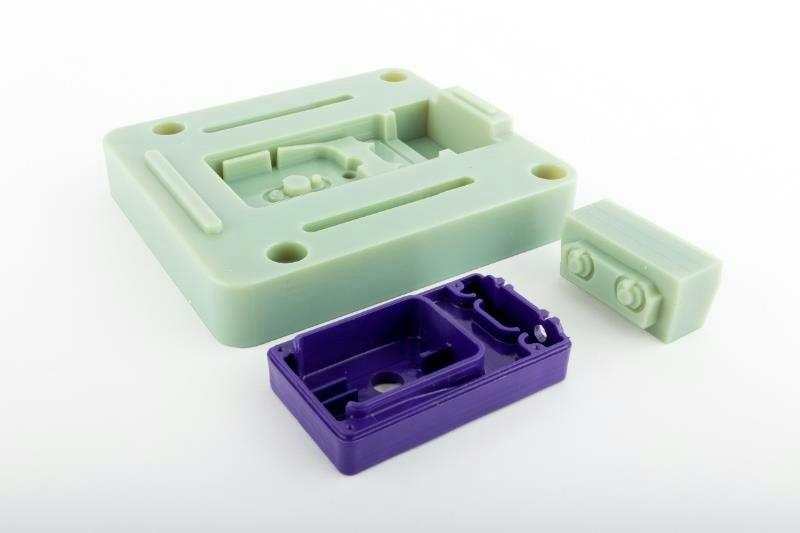
\includegraphics[width=441.9pt,height=294.6pt]{latexImage_d46859ed68c22a3bf5d30a453c1eaaec.png}}
\end{picture}
\newpage
\begin{tikzpicture}[overlay]\path(0pt,0pt);\end{tikzpicture}
\begin{picture}(-5,0)(2.5,0)
\put(500.14,-727.616){\fontsize{12}{1}\usefont{T1}{ptm}{m}{n}\selectfont\color{color_29791}20}
\put(512.14,-727.616){\fontsize{12}{1}\usefont{T1}{ptm}{m}{n}\selectfont\color{color_29791} }
\put(515.14,-727.616){\fontsize{12}{1}\usefont{T1}{ptm}{m}{n}\selectfont\color{color_29791} }
\put(70.104,-742.496){\fontsize{10.56}{1}\usefont{T1}{ptm}{m}{n}\selectfont\color{color_29791} }
\put(72.744,-742.496){\fontsize{12}{1}\usefont{T1}{ptm}{m}{n}\selectfont\color{color_29791} }
\put(515.74,-386.77){\fontsize{12}{1}\usefont{T1}{ptm}{m}{n}\selectfont\color{color_29791} }
\put(518.74,-386.77){\fontsize{12}{1}\usefont{T1}{ptm}{m}{n}\selectfont\color{color_29791} }
\put(222.05,-409.33){\fontsize{12}{1}\usefont{T1}{ptm}{m}{n}\selectfont\color{color_29791}圖}
\put(234.17,-409.33){\fontsize{12}{1}\usefont{T1}{ptm}{b}{n}\selectfont\color{color_29791}13 }
\put(249.05,-409.33){\fontsize{12}{1}\usefont{T1}{ptm}{m}{n}\selectfont\color{color_29791}理論乘}
\put(285.158,-409.33){\fontsize{12}{1}\usefont{T1}{ptm}{m}{n}\selectfont\color{color_29791}積的}
\put(309.29,-409.33){\fontsize{12}{1}\usefont{T1}{ptm}{b}{n}\selectfont\color{color_29791}3}
\put(315.31,-409.33){\fontsize{12}{1}\usefont{T1}{ptm}{b}{n}\selectfont\color{color_29791}D}
\put(323.83,-409.33){\fontsize{12}{1}\usefont{T1}{ptm}{m}{n}\selectfont\color{color_29791}分解圖}
\put(359.95,-409.33){\fontsize{12}{1}\usefont{T1}{ptm}{b}{n}\selectfont\color{color_29791} }
\put(362.83,-409.33){\fontsize{12}{1}\usefont{T1}{ptm}{m}{n}\selectfont\color{color_29791} }
\put(70.104,-426.63){\fontsize{12}{1}\usefont{T1}{ptm}{m}{n}\selectfont\color{color_29791} }
\put(73.104,-426.63){\fontsize{12}{1}\usefont{T1}{ptm}{m}{n}\selectfont\color{color_29791} }
\put(105.38,-464.07){\fontsize{12.96}{1}\usefont{T1}{ptm}{b}{n}\selectfont\color{color_29791}4.1.1. }
\put(137.0542,-464.07){\fontsize{12.96}{1}\usefont{T1}{ptm}{b}{n}\selectfont\color{color_29791}A}
\put(146.42,-464.07){\fontsize{12.96}{1}\usefont{T1}{ptm}{m}{n}\selectfont\color{color_29791}部分}
\put(172.58,-464.07){\fontsize{12.96}{1}\usefont{T1}{ptm}{b}{n}\selectfont\color{color_29791} }
\put(175.82,-464.07){\fontsize{12.96}{1}\usefont{T1}{ptm}{b}{n}\selectfont\color{color_29791} }
\put(82.944,-492.75){\fontsize{12}{1}\usefont{T1}{ptm}{m}{n}\selectfont\color{color_29791}P}
\put(88.584,-492.75){\fontsize{12}{1}\usefont{T1}{ptm}{m}{n}\selectfont\color{color_29791}AR}
\put(104.544,-492.75){\fontsize{12}{1}\usefont{T1}{ptm}{m}{n}\selectfont\color{color_29791}T}
\put(110.78,-492.75){\fontsize{12}{1}\usefont{T1}{ptm}{m}{n}\selectfont\color{color_29791}-}
\put(69.384,-508.59){\fontsize{12}{1}\usefont{T1}{ptm}{m}{n}\selectfont\color{color_29791}A}
\put(78.024,-508.59){\fontsize{12}{1}\usefont{T1}{ptm}{m}{n}\selectfont\color{color_29791}(}
\put(90.02,-508.59){\fontsize{12}{1}\usefont{T1}{ptm}{m}{n}\selectfont\color{color_29791}圖}
\put(102.02,-508.59){\fontsize{12}{1}\usefont{T1}{ptm}{m}{n}\selectfont\color{color_29791}14}
\put(114.02,-508.59){\fontsize{12}{1}\usefont{T1}{ptm}{m}{n}\selectfont\color{color_29791})}
\put(126.02,-508.59){\fontsize{12}{1}\usefont{T1}{ptm}{m}{n}\selectfont\color{color_29791}是計算機機箱的核心結構}
\put(258.05,-508.59){\fontsize{12}{1}\usefont{T1}{ptm}{m}{n}\selectfont\color{color_29791}。}
\put(270.05,-508.59){\fontsize{12}{1}\usefont{T1}{ptm}{m}{n}\selectfont\color{color_29791}預計它將包含所討論的小型電腦正常運行所需}
\put(69.384,-526.23){\fontsize{12}{1}\usefont{T1}{ptm}{m}{n}\selectfont\color{color_29791}的所有部件}
\put(129.38,-526.23){\fontsize{12}{1}\usefont{T1}{ptm}{m}{n}\selectfont\color{color_29791}。}
\put(141.38,-526.23){\fontsize{12}{1}\usefont{T1}{ptm}{m}{n}\selectfont\color{color_29791}為此}
\put(165.38,-526.23){\fontsize{12}{1}\usefont{T1}{ptm}{m}{n}\selectfont\color{color_29791},}
\put(177.38,-526.23){\fontsize{12}{1}\usefont{T1}{ptm}{m}{n}\selectfont\color{color_29791}選擇了一種原料}
\put(261.41,-526.23){\fontsize{12}{1}\usefont{T1}{ptm}{m}{n}\selectfont\color{color_29791}A}
\put(270.05,-526.23){\fontsize{12}{1}\usefont{T1}{ptm}{m}{n}\selectfont\color{color_29791},}
\put(282.05,-526.23){\fontsize{12}{1}\usefont{T1}{ptm}{m}{n}\selectfont\color{color_29791}即丙烯腈丁二烯苯乙烯}
\put(402.07,-526.23){\fontsize{12}{1}\usefont{T1}{ptm}{m}{n}\selectfont\color{color_29791}(}
\put(414.07,-526.23){\fontsize{12}{1}\usefont{T1}{ptm}{m}{n}\selectfont\color{color_29791}AB}
\put(430.63,-526.23){\fontsize{12}{1}\usefont{T1}{ptm}{m}{n}\selectfont\color{color_29791}S}
\put(437.35,-526.23){\fontsize{12}{1}\usefont{T1}{ptm}{m}{n}\selectfont\color{color_29791}),}
\put(461.38,-526.23){\fontsize{12}{1}\usefont{T1}{ptm}{m}{n}\selectfont\color{color_29791}這是一種}
\put(69.384,-543.87){\fontsize{12}{1}\usefont{T1}{ptm}{m}{n}\selectfont\color{color_29791}不透明的熱塑性聚合物和工程級塑膠}
\put(261.41,-543.87){\fontsize{12}{1}\usefont{T1}{ptm}{m}{n}\selectfont\color{color_29791}。}
\put(273.41,-543.87){\fontsize{12}{1}\usefont{T1}{ptm}{m}{n}\selectfont\color{color_29791}它通常用於生產電子零件}
\put(405.43,-543.87){\fontsize{12}{1}\usefont{T1}{ptm}{m}{n}\selectfont\color{color_29791},}
\put(417.43,-543.87){\fontsize{12}{1}\usefont{T1}{ptm}{m}{n}\selectfont\color{color_29791}如手機適配器}
\put(489.46,-543.87){\fontsize{12}{1}\usefont{T1}{ptm}{m}{n}\selectfont\color{color_29791}、}
\put(69.384,-561.63){\fontsize{12}{1}\usefont{T1}{ptm}{m}{n}\selectfont\color{color_29791}鍵盤鍵和牆壁插座塑膠護罩}
\put(213.41,-561.63){\fontsize{12}{1}\usefont{T1}{ptm}{m}{n}\selectfont\color{color_29791}。}
\put(225.41,-561.63){\fontsize{12}{1}\usefont{T1}{ptm}{m}{n}\selectfont\color{color_29791}  }
\put(231.41,-561.63){\fontsize{12}{1}\usefont{T1}{ptm}{m}{n}\selectfont\color{color_29791} }
\put(73.75,-386.65){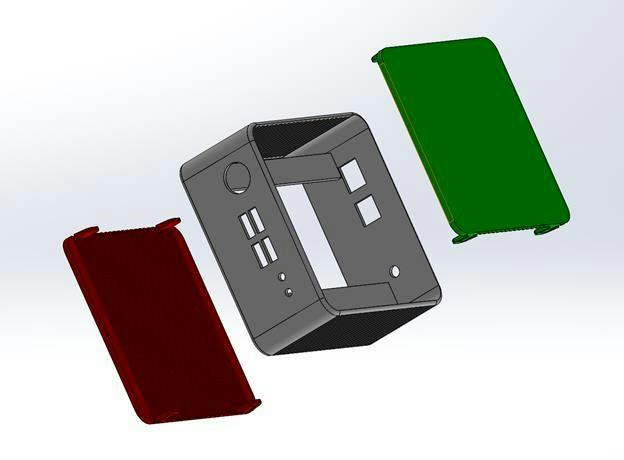
\includegraphics[width=441.9pt,height=325.75pt]{latexImage_a09d404156753daa5ee7b8542e464588.png}}
\end{picture}
\newpage
\begin{tikzpicture}[overlay]\path(0pt,0pt);\end{tikzpicture}
\begin{picture}(-5,0)(2.5,0)
\put(500.14,-727.616){\fontsize{12}{1}\usefont{T1}{ptm}{m}{n}\selectfont\color{color_29791}21}
\put(512.14,-727.616){\fontsize{12}{1}\usefont{T1}{ptm}{m}{n}\selectfont\color{color_29791} }
\put(515.14,-727.616){\fontsize{12}{1}\usefont{T1}{ptm}{m}{n}\selectfont\color{color_29791} }
\put(70.104,-742.496){\fontsize{10.56}{1}\usefont{T1}{ptm}{m}{n}\selectfont\color{color_29791} }
\put(72.744,-742.496){\fontsize{12}{1}\usefont{T1}{ptm}{m}{n}\selectfont\color{color_29791} }
\put(529.9,-267.73){\fontsize{12}{1}\usefont{T1}{ptm}{m}{n}\selectfont\color{color_29791} }
\put(532.9,-267.73){\fontsize{12}{1}\usefont{T1}{ptm}{m}{n}\selectfont\color{color_29791} }
\put(220.97,-280.21){\fontsize{12}{1}\usefont{T1}{ptm}{m}{n}\selectfont\color{color_29791}圖}
\put(233.09,-280.21){\fontsize{12}{1}\usefont{T1}{ptm}{b}{n}\selectfont\color{color_29791} }
\put(236.09,-280.21){\fontsize{12}{1}\usefont{T1}{ptm}{b}{n}\selectfont\color{color_29791}14 }
\put(250.97,-280.21){\fontsize{12}{1}\usefont{T1}{ptm}{m}{n}\selectfont\color{color_29791}零件}
\put(275.09,-280.21){\fontsize{12}{1}\usefont{T1}{ptm}{b}{n}\selectfont\color{color_29791} }
\put(278.09,-280.21){\fontsize{12}{1}\usefont{T1}{ptm}{b}{n}\selectfont\color{color_29791}A }
\put(289.01,-280.21){\fontsize{12}{1}\usefont{T1}{ptm}{m}{n}\selectfont\color{color_29791}的等軸測檢視}
\put(361.15,-280.21){\fontsize{12}{1}\usefont{T1}{ptm}{b}{n}\selectfont\color{color_29791} }
\put(364.03,-280.21){\fontsize{12}{1}\usefont{T1}{ptm}{m}{n}\selectfont\color{color_29791} }
\put(70.104,-297.49){\fontsize{12}{1}\usefont{T1}{ptm}{m}{n}\selectfont\color{color_29791} }
\put(73.104,-297.49){\fontsize{12}{1}\usefont{T1}{ptm}{m}{n}\selectfont\color{color_29791} }
\put(82.944,-312.61){\fontsize{12}{1}\usefont{T1}{ptm}{m}{n}\selectfont\color{color_29791}特別選擇這種材料的主要原因是它的韌性}
\put(298.97,-312.61){\fontsize{12}{1}\usefont{T1}{ptm}{m}{n}\selectfont\color{color_29791}、}
\put(310.97,-312.61){\fontsize{12}{1}\usefont{T1}{ptm}{m}{n}\selectfont\color{color_29791}良好的尺寸穩定性}
\put(406.99,-312.61){\fontsize{12}{1}\usefont{T1}{ptm}{m}{n}\selectfont\color{color_29791}(}
\put(418.99,-312.61){\fontsize{12}{1}\usefont{T1}{ptm}{m}{n}\selectfont\color{color_29791}冷卻后不改變尺}
\put(69.384,-330.25){\fontsize{12}{1}\usefont{T1}{ptm}{m}{n}\selectfont\color{color_29791}寸}
\put(81.384,-330.25){\fontsize{12}{1}\usefont{T1}{ptm}{m}{n}\selectfont\color{color_29791})、}
\put(105.38,-330.25){\fontsize{12}{1}\usefont{T1}{ptm}{m}{n}\selectfont\color{color_29791}高抗衝擊性和表面硬度}
\put(225.41,-330.25){\fontsize{12}{1}\usefont{T1}{ptm}{m}{n}\selectfont\color{color_29791}。}
\put(237.41,-330.25){\fontsize{12}{1}\usefont{T1}{ptm}{m}{n}\selectfont\color{color_29791}最後}
\put(261.41,-330.25){\fontsize{12}{1}\usefont{T1}{ptm}{m}{n}\selectfont\color{color_29791},}
\put(273.41,-330.25){\fontsize{12}{1}\usefont{T1}{ptm}{m}{n}\selectfont\color{color_29791}它通常也以}
\put(333.43,-330.25){\fontsize{12}{1}\usefont{T1}{ptm}{m}{n}\selectfont\color{color_29791}3}
\put(339.43,-330.25){\fontsize{12}{1}\usefont{T1}{ptm}{m}{n}\selectfont\color{color_29791}D}
\put(348.07,-330.25){\fontsize{12}{1}\usefont{T1}{ptm}{m}{n}\selectfont\color{color_29791}列印長絲的形式用於擠出}
\put(480.1,-330.25){\fontsize{12}{1}\usefont{T1}{ptm}{m}{n}\selectfont\color{color_29791}3}
\put(486.1,-330.25){\fontsize{12}{1}\usefont{T1}{ptm}{m}{n}\selectfont\color{color_29791}D}
\put(494.74,-330.25){\fontsize{12}{1}\usefont{T1}{ptm}{m}{n}\selectfont\color{color_29791}印}
\put(69.384,-348.01){\fontsize{12}{1}\usefont{T1}{ptm}{m}{n}\selectfont\color{color_29791}表機}
\put(93.38,-348.01){\fontsize{12}{1}\usefont{T1}{ptm}{m}{n}\selectfont\color{color_29791},}
\put(105.38,-348.01){\fontsize{12}{1}\usefont{T1}{ptm}{m}{n}\selectfont\color{color_29791}這應該在原型製作過程中被證明非常有用}
\put(321.43,-348.01){\fontsize{12}{1}\usefont{T1}{ptm}{m}{n}\selectfont\color{color_29791}。}
\put(333.43,-348.01){\fontsize{12}{1}\usefont{T1}{ptm}{m}{n}\selectfont\color{color_29791}  }
\put(339.43,-348.01){\fontsize{12}{1}\usefont{T1}{ptm}{m}{n}\selectfont\color{color_29791} }
\put(84.264,-365.53){\fontsize{12}{1}\usefont{T1}{ptm}{m}{n}\selectfont\color{color_29791} }
\put(87.26,-365.53){\fontsize{12}{1}\usefont{T1}{ptm}{m}{n}\selectfont\color{color_29791} }
\put(105.38,-405.01){\fontsize{12.96}{1}\usefont{T1}{ptm}{b}{n}\selectfont\color{color_29791}4.1.2. B }
\put(149.66,-405.01){\fontsize{12.96}{1}\usefont{T1}{ptm}{m}{n}\selectfont\color{color_29791}和}
\put(162.74,-405.01){\fontsize{12.96}{1}\usefont{T1}{ptm}{b}{n}\selectfont\color{color_29791} }
\put(165.98,-405.01){\fontsize{12.96}{1}\usefont{T1}{ptm}{b}{n}\selectfont\color{color_29791}C }
\put(178.58,-405.01){\fontsize{12.96}{1}\usefont{T1}{ptm}{m}{n}\selectfont\color{color_29791}部分}
\put(204.77,-405.01){\fontsize{12.96}{1}\usefont{T1}{ptm}{b}{n}\selectfont\color{color_29791} }
\put(208.01,-405.01){\fontsize{12.96}{1}\usefont{T1}{ptm}{b}{n}\selectfont\color{color_29791} }
\put(82.944,-434.07){\fontsize{12}{1}\usefont{T1}{ptm}{m}{n}\selectfont\color{color_29791}B }
\put(291.77,-434.07){\fontsize{12}{1}\usefont{T1}{ptm}{m}{n}\selectfont\color{color_29791}和}
\put(303.77,-434.07){\fontsize{12}{1}\usefont{T1}{ptm}{m}{n}\selectfont\color{color_29791} }
\put(504.58,-434.07){\fontsize{12}{1}\usefont{T1}{ptm}{m}{n}\selectfont\color{color_29791}C }
\put(69.384,-451.59){\fontsize{12}{1}\usefont{T1}{ptm}{m}{n}\selectfont\color{color_29791}部分是蓋子}
\put(129.38,-451.59){\fontsize{12}{1}\usefont{T1}{ptm}{m}{n}\selectfont\color{color_29791},}
\put(141.38,-451.59){\fontsize{12}{1}\usefont{T1}{ptm}{m}{n}\selectfont\color{color_29791}應卡入到位}
\put(201.41,-451.59){\fontsize{12}{1}\usefont{T1}{ptm}{m}{n}\selectfont\color{color_29791},}
\put(213.41,-451.59){\fontsize{12}{1}\usefont{T1}{ptm}{m}{n}\selectfont\color{color_29791}關閉系統}
\put(261.41,-451.59){\fontsize{12}{1}\usefont{T1}{ptm}{m}{n}\selectfont\color{color_29791}。}
\put(273.41,-451.59){\fontsize{12}{1}\usefont{T1}{ptm}{m}{n}\selectfont\color{color_29791}這些是非常簡單的部件}
\put(393.43,-451.59){\fontsize{12}{1}\usefont{T1}{ptm}{m}{n}\selectfont\color{color_29791},}
\put(405.43,-451.59){\fontsize{12}{1}\usefont{T1}{ptm}{m}{n}\selectfont\color{color_29791}需要一定程度的彈}
\put(69.384,-469.23){\fontsize{12}{1}\usefont{T1}{ptm}{m}{n}\selectfont\color{color_29791}性}
\put(81.384,-469.23){\fontsize{12}{1}\usefont{T1}{ptm}{m}{n}\selectfont\color{color_29791},}
\put(93.38,-469.23){\fontsize{12}{1}\usefont{T1}{ptm}{m}{n}\selectfont\color{color_29791}因此它可以變形以確保無螺絲組裝}
\put(273.41,-469.23){\fontsize{12}{1}\usefont{T1}{ptm}{m}{n}\selectfont\color{color_29791}。}
\put(285.41,-469.23){\fontsize{12}{1}\usefont{T1}{ptm}{m}{n}\selectfont\color{color_29791}這兩個相同的部件將由熱塑性聚氨酯}
\put(477.46,-469.23){\fontsize{12}{1}\usefont{T1}{ptm}{m}{n}\selectfont\color{color_29791} }
\put(69.384,-486.87){\fontsize{12}{1}\usefont{T1}{ptm}{m}{n}\selectfont\color{color_29791}(}
\put(81.384,-486.87){\fontsize{12}{1}\usefont{T1}{ptm}{m}{n}\selectfont\color{color_29791}TP}
\put(95.412,-486.87){\fontsize{12}{1}\usefont{T1}{ptm}{m}{n}\selectfont\color{color_29791}U}
\put(104.06,-486.87){\fontsize{12}{1}\usefont{T1}{ptm}{m}{n}\selectfont\color{color_29791})}
\put(116.06,-486.87){\fontsize{12}{1}\usefont{T1}{ptm}{m}{n}\selectfont\color{color_29791} }
\put(248.57,-486.87){\fontsize{12}{1}\usefont{T1}{ptm}{m}{n}\selectfont\color{color_29791}製成}
\put(272.57,-486.87){\fontsize{12}{1}\usefont{T1}{ptm}{m}{n}\selectfont\color{color_29791},}
\put(284.57,-486.87){\fontsize{12}{1}\usefont{T1}{ptm}{m}{n}\selectfont\color{color_29791}因為它具有彈性和出色的拉伸和撕裂強度}
\put(500.62,-486.87){\fontsize{12}{1}\usefont{T1}{ptm}{m}{n}\selectfont\color{color_29791}。}
\put(512.5,-486.87){\fontsize{12}{1}\usefont{T1}{ptm}{m}{n}\selectfont\color{color_29791} }
\put(69.384,-504.51){\fontsize{12}{1}\usefont{T1}{ptm}{m}{n}\selectfont\color{color_29791}這種聚合物通常用於生產需要類似橡膠彈性的零件}
\put(333.43,-504.51){\fontsize{12}{1}\usefont{T1}{ptm}{m}{n}\selectfont\color{color_29791}。}
\put(345.43,-504.51){\fontsize{12}{1}\usefont{T1}{ptm}{m}{n}\selectfont\color{color_29791}熱塑性聚氨酯在高溫下表現良}
\put(69.384,-522.15){\fontsize{12}{1}\usefont{T1}{ptm}{m}{n}\selectfont\color{color_29791}好}
\put(81.384,-522.15){\fontsize{12}{1}\usefont{T1}{ptm}{m}{n}\selectfont\color{color_29791},}
\put(93.38,-522.15){\fontsize{12}{1}\usefont{T1}{ptm}{m}{n}\selectfont\color{color_29791}常用於電動工具}
\put(177.38,-522.15){\fontsize{12}{1}\usefont{T1}{ptm}{m}{n}\selectfont\color{color_29791}、}
\put(189.41,-522.15){\fontsize{12}{1}\usefont{T1}{ptm}{m}{n}\selectfont\color{color_29791}電纜絕緣層和體育用品}
\put(309.41,-522.15){\fontsize{12}{1}\usefont{T1}{ptm}{m}{n}\selectfont\color{color_29791}。}
\put(321.43,-522.15){\fontsize{12}{1}\usefont{T1}{ptm}{m}{n}\selectfont\color{color_29791}最後}
\put(345.43,-522.15){\fontsize{12}{1}\usefont{T1}{ptm}{m}{n}\selectfont\color{color_29791},}
\put(357.43,-522.15){\fontsize{12}{1}\usefont{T1}{ptm}{m}{n}\selectfont\color{color_29791}TP}
\put(371.458,-522.15){\fontsize{12}{1}\usefont{T1}{ptm}{m}{n}\selectfont\color{color_29791}U}
\put(380.11,-522.15){\fontsize{12}{1}\usefont{T1}{ptm}{m}{n}\selectfont\color{color_29791}還以長絲的形式提供}
\put(488.14,-522.15){\fontsize{12}{1}\usefont{T1}{ptm}{m}{n}\selectfont\color{color_29791},}
\put(500.14,-522.15){\fontsize{12}{1}\usefont{T1}{ptm}{m}{n}\selectfont\color{color_29791}用}
\put(69.384,-539.91){\fontsize{12}{1}\usefont{T1}{ptm}{m}{n}\selectfont\color{color_29791}於}
\put(81.384,-539.91){\fontsize{12}{1}\usefont{T1}{ptm}{m}{n}\selectfont\color{color_29791}3}
\put(87.38,-539.91){\fontsize{12}{1}\usefont{T1}{ptm}{m}{n}\selectfont\color{color_29791}D}
\put(96.02,-539.91){\fontsize{12}{1}\usefont{T1}{ptm}{m}{n}\selectfont\color{color_29791}印表機}
\put(132.02,-539.91){\fontsize{12}{1}\usefont{T1}{ptm}{m}{n}\selectfont\color{color_29791},}
\put(144.02,-539.91){\fontsize{12}{1}\usefont{T1}{ptm}{m}{n}\selectfont\color{color_29791}用於類比}
\put(192.05,-539.91){\fontsize{12}{1}\usefont{T1}{ptm}{m}{n}\selectfont\color{color_29791},}
\put(204.05,-539.91){\fontsize{12}{1}\usefont{T1}{ptm}{m}{n}\selectfont\color{color_29791}將用於原型製作}
\put(288.05,-539.91){\fontsize{12}{1}\usefont{T1}{ptm}{m}{n}\selectfont\color{color_29791}。}
\put(300.05,-539.91){\fontsize{12}{1}\usefont{T1}{ptm}{m}{n}\selectfont\color{color_29791}  }
\put(306.05,-539.91){\fontsize{12}{1}\usefont{T1}{ptm}{m}{n}\selectfont\color{color_29791} }
\put(87.9,-267.65){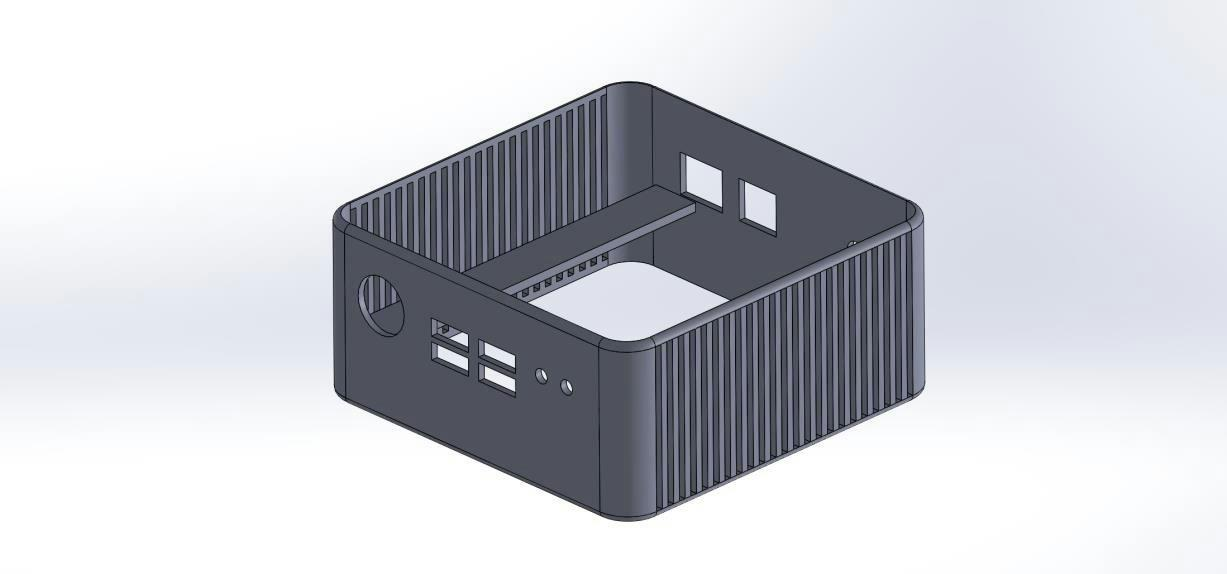
\includegraphics[width=441.9pt,height=206.75pt]{latexImage_bb37b80ab42df558373dcc5c79567809.png}}
\end{picture}
\newpage
\begin{tikzpicture}[overlay]\path(0pt,0pt);\end{tikzpicture}
\begin{picture}(-5,0)(2.5,0)
\put(500.14,-727.616){\fontsize{12}{1}\usefont{T1}{ptm}{m}{n}\selectfont\color{color_29791}22}
\put(512.14,-727.616){\fontsize{12}{1}\usefont{T1}{ptm}{m}{n}\selectfont\color{color_29791} }
\put(515.14,-727.616){\fontsize{12}{1}\usefont{T1}{ptm}{m}{n}\selectfont\color{color_29791} }
\put(70.104,-742.496){\fontsize{10.56}{1}\usefont{T1}{ptm}{m}{n}\selectfont\color{color_29791} }
\put(72.744,-742.496){\fontsize{12}{1}\usefont{T1}{ptm}{m}{n}\selectfont\color{color_29791} }
\put(529.9,-262.69){\fontsize{12}{1}\usefont{T1}{ptm}{m}{n}\selectfont\color{color_29791} }
\put(532.9,-262.69){\fontsize{12}{1}\usefont{T1}{ptm}{m}{n}\selectfont\color{color_29791} }
\put(245.09,-275.05){\fontsize{12}{1}\usefont{T1}{ptm}{m}{n}\selectfont\color{color_29791}圖}
\put(257.21,-275.05){\fontsize{12}{1}\usefont{T1}{ptm}{b}{n}\selectfont\color{color_29791} }
\put(260.21,-275.05){\fontsize{12}{1}\usefont{T1}{ptm}{b}{n}\selectfont\color{color_29791}15 }
\put(275.21,-275.05){\fontsize{12}{1}\usefont{T1}{ptm}{b}{n}\selectfont\color{color_29791}B }
\put(286.13,-275.05){\fontsize{12}{1}\usefont{T1}{ptm}{m}{n}\selectfont\color{color_29791}和}
\put(298.25,-275.05){\fontsize{12}{1}\usefont{T1}{ptm}{b}{n}\selectfont\color{color_29791} }
\put(301.25,-275.05){\fontsize{12}{1}\usefont{T1}{ptm}{b}{n}\selectfont\color{color_29791}C }
\put(312.79,-275.05){\fontsize{12}{1}\usefont{T1}{ptm}{m}{n}\selectfont\color{color_29791}部分}
\put(336.91,-275.05){\fontsize{12}{1}\usefont{T1}{ptm}{b}{n}\selectfont\color{color_29791} }
\put(339.79,-275.05){\fontsize{12}{1}\usefont{T1}{ptm}{m}{n}\selectfont\color{color_29791} }
\put(105.38,-314.41){\fontsize{12.96}{1}\usefont{T1}{ptm}{b}{n}\selectfont\color{color_29791}4.1.3. }
\put(137.78,-314.41){\fontsize{12.96}{1}\usefont{T1}{ptm}{m}{n}\selectfont\color{color_29791}模具}
\put(163.94,-314.41){\fontsize{12.96}{1}\usefont{T1}{ptm}{b}{n}\selectfont\color{color_29791}  }
\put(170.42,-314.41){\fontsize{12.96}{1}\usefont{T1}{ptm}{b}{n}\selectfont\color{color_29791} }
\put(82.944,-343.33){\fontsize{12}{1}\usefont{T1}{ptm}{m}{n}\selectfont\color{color_29791}理想情況下}
\put(142.94,-343.33){\fontsize{12}{1}\usefont{T1}{ptm}{m}{n}\selectfont\color{color_29791},}
\put(154.94,-343.33){\fontsize{12}{1}\usefont{T1}{ptm}{m}{n}\selectfont\color{color_29791}所有模具都應由鋼製成}
\put(274.97,-343.33){\fontsize{12}{1}\usefont{T1}{ptm}{m}{n}\selectfont\color{color_29791},}
\put(286.97,-343.33){\fontsize{12}{1}\usefont{T1}{ptm}{m}{n}\selectfont\color{color_29791}以延長模具的使用壽命和產品品質}
\put(467.02,-343.33){\fontsize{12}{1}\usefont{T1}{ptm}{m}{n}\selectfont\color{color_29791}。}
\put(479.02,-343.33){\fontsize{12}{1}\usefont{T1}{ptm}{m}{n}\selectfont\color{color_29791}話雖}
\put(69.384,-360.97){\fontsize{12}{1}\usefont{T1}{ptm}{m}{n}\selectfont\color{color_29791}如此}
\put(93.38,-360.97){\fontsize{12}{1}\usefont{T1}{ptm}{m}{n}\selectfont\color{color_29791},}
\put(105.38,-360.97){\fontsize{12}{1}\usefont{T1}{ptm}{m}{n}\selectfont\color{color_29791}為所有零件選擇的注塑塑膠與壓力無關}
\put(309.41,-360.97){\fontsize{12}{1}\usefont{T1}{ptm}{m}{n}\selectfont\color{color_29791},}
\put(321.43,-360.97){\fontsize{12}{1}\usefont{T1}{ptm}{m}{n}\selectfont\color{color_29791}其形式也不那麼複雜}
\put(429.43,-360.97){\fontsize{12}{1}\usefont{T1}{ptm}{m}{n}\selectfont\color{color_29791},}
\put(441.43,-360.97){\fontsize{12}{1}\usefont{T1}{ptm}{m}{n}\selectfont\color{color_29791}因此假設用}
\put(69.384,-378.73){\fontsize{12}{1}\usefont{T1}{ptm}{m}{n}\selectfont\color{color_29791}精密}
\put(93.38,-378.73){\fontsize{12}{1}\usefont{T1}{ptm}{m}{n}\selectfont\color{color_29791} }
\put(96.38,-378.73){\fontsize{12}{1}\usefont{T1}{ptm}{m}{n}\selectfont\color{color_29791}C}
\put(104.408,-378.73){\fontsize{12}{1}\usefont{T1}{ptm}{m}{n}\selectfont\color{color_29791}NC }
\put(124.1,-378.73){\fontsize{12}{1}\usefont{T1}{ptm}{m}{n}\selectfont\color{color_29791}加工製成的鋁模具應該足以生產上述零件}
\put(340.15,-378.73){\fontsize{12}{1}\usefont{T1}{ptm}{m}{n}\selectfont\color{color_29791}。}
\put(352.15,-378.73){\fontsize{12}{1}\usefont{T1}{ptm}{m}{n}\selectfont\color{color_29791} }
\put(355.15,-378.73){\fontsize{12}{1}\usefont{T1}{ptm}{m}{n}\selectfont\color{color_29791} }
\put(84.264,-396.13){\fontsize{12}{1}\usefont{T1}{ptm}{m}{n}\selectfont\color{color_29791} }
\put(87.26,-396.13){\fontsize{12}{1}\usefont{T1}{ptm}{m}{n}\selectfont\color{color_29791} }
\put(82.944,-412.21){\fontsize{12}{1}\usefont{T1}{ptm}{m}{n}\selectfont\color{color_29791}還假設所有模具都足夠簡單}
\put(226.97,-412.21){\fontsize{12}{1}\usefont{T1}{ptm}{m}{n}\selectfont\color{color_29791},}
\put(238.97,-412.21){\fontsize{12}{1}\usefont{T1}{ptm}{m}{n}\selectfont\color{color_29791}可以使用}
\put(286.97,-412.21){\fontsize{12}{1}\usefont{T1}{ptm}{m}{n}\selectfont\color{color_29791}3}
\put(292.97,-412.21){\fontsize{12}{1}\usefont{T1}{ptm}{m}{n}\selectfont\color{color_29791}D}
\put(301.61,-412.21){\fontsize{12}{1}\usefont{T1}{ptm}{m}{n}\selectfont\color{color_29791}列印進行原型設計}
\put(397.63,-412.21){\fontsize{12}{1}\usefont{T1}{ptm}{m}{n}\selectfont\color{color_29791}。}
\put(409.63,-412.21){\fontsize{12}{1}\usefont{T1}{ptm}{m}{n}\selectfont\color{color_29791}雖然這並不總是正}
\put(69.384,-429.75){\fontsize{12}{1}\usefont{T1}{ptm}{m}{n}\selectfont\color{color_29791}確的}
\put(93.38,-429.75){\fontsize{12}{1}\usefont{T1}{ptm}{m}{n}\selectfont\color{color_29791},}
\put(105.38,-429.75){\fontsize{12}{1}\usefont{T1}{ptm}{m}{n}\selectfont\color{color_29791}但對於這個模擬來說}
\put(213.41,-429.75){\fontsize{12}{1}\usefont{T1}{ptm}{m}{n}\selectfont\color{color_29791},}
\put(225.41,-429.75){\fontsize{12}{1}\usefont{T1}{ptm}{m}{n}\selectfont\color{color_29791}它被確定為足夠的代表性}
\put(357.43,-429.75){\fontsize{12}{1}\usefont{T1}{ptm}{m}{n}\selectfont\color{color_29791}。}
\put(369.43,-429.75){\fontsize{12}{1}\usefont{T1}{ptm}{m}{n}\selectfont\color{color_29791}這些原型中使用的材料類}
\put(69.384,-447.39){\fontsize{12}{1}\usefont{T1}{ptm}{m}{n}\selectfont\color{color_29791}型是使用}
\put(117.38,-447.39){\fontsize{12}{1}\usefont{T1}{ptm}{m}{n}\selectfont\color{color_29791} }
\put(280.25,-447.39){\fontsize{12}{1}\usefont{T1}{ptm}{m}{n}\selectfont\color{color_29791}S}
\put(287.078,-447.39){\fontsize{12}{1}\usefont{T1}{ptm}{m}{n}\selectfont\color{color_29791}L}
\put(294.158,-447.39){\fontsize{12}{1}\usefont{T1}{ptm}{m}{n}\selectfont\color{color_29791}A}
\put(302.198,-447.39){\fontsize{12}{1}\usefont{T1}{ptm}{m}{n}\selectfont\color{color_29791} }
\put(465.05,-447.39){\fontsize{12}{1}\usefont{T1}{ptm}{m}{n}\selectfont\color{color_29791}3DPrint}
\put(503.078,-447.39){\fontsize{12}{1}\usefont{T1}{ptm}{m}{n}\selectfont\color{color_29791}e}
\put(508.358,-447.39){\fontsize{12}{1}\usefont{T1}{ptm}{m}{n}\selectfont\color{color_29791}r}
\put(512.426,-447.39){\fontsize{12}{1}\usefont{T1}{ptm}{m}{n}\selectfont\color{color_29791} }
\put(69.384,-465.03){\fontsize{12}{1}\usefont{T1}{ptm}{m}{n}\selectfont\color{color_29791}固化的高溫退膠}
\put(153.38,-465.03){\fontsize{12}{1}\usefont{T1}{ptm}{m}{n}\selectfont\color{color_29791}。}
\put(165.38,-465.03){\fontsize{12}{1}\usefont{T1}{ptm}{m}{n}\selectfont\color{color_29791}此外}
\put(189.41,-465.03){\fontsize{12}{1}\usefont{T1}{ptm}{m}{n}\selectfont\color{color_29791},}
\put(201.41,-465.03){\fontsize{12}{1}\usefont{T1}{ptm}{m}{n}\selectfont\color{color_29791}在生產過程中}
\put(273.41,-465.03){\fontsize{12}{1}\usefont{T1}{ptm}{m}{n}\selectfont\color{color_29791},}
\put(285.41,-465.03){\fontsize{12}{1}\usefont{T1}{ptm}{m}{n}\selectfont\color{color_29791}模具將被視為要開發的主要物理方面}
\put(477.46,-465.03){\fontsize{12}{1}\usefont{T1}{ptm}{m}{n}\selectfont\color{color_29791},}
\put(489.46,-465.03){\fontsize{12}{1}\usefont{T1}{ptm}{m}{n}\selectfont\color{color_29791}因}
\put(69.384,-482.79){\fontsize{12}{1}\usefont{T1}{ptm}{m}{n}\selectfont\color{color_29791}為它直接影響生產}
\put(165.38,-482.79){\fontsize{12}{1}\usefont{T1}{ptm}{m}{n}\selectfont\color{color_29791},}
\put(177.38,-482.79){\fontsize{12}{1}\usefont{T1}{ptm}{m}{n}\selectfont\color{color_29791}並且可以在內部生產並像產品一樣進行跟蹤}
\put(405.43,-482.79){\fontsize{12}{1}\usefont{T1}{ptm}{m}{n}\selectfont\color{color_29791}。}
\put(417.43,-482.79){\fontsize{12}{1}\usefont{T1}{ptm}{m}{n}\selectfont\color{color_29791}  }
\put(423.43,-482.79){\fontsize{12}{1}\usefont{T1}{ptm}{m}{n}\selectfont\color{color_29791} }
\put(70.104,-500.31){\fontsize{12}{1}\usefont{T1}{ptm}{m}{n}\selectfont\color{color_29791} }
\put(73.104,-500.31){\fontsize{12}{1}\usefont{T1}{ptm}{m}{n}\selectfont\color{color_29791} }
\put(87.38,-532.71){\fontsize{14.04}{1}\usefont{T1}{ptm}{b}{n}\selectfont\color{color_29791}4}
\put(94.44212,-532.71){\fontsize{14.04}{1}\usefont{T1}{ptm}{b}{n}\selectfont\color{color_29791}.2. }
\put(111.86,-532.71){\fontsize{14.04}{1}\usefont{T1}{ptm}{m}{n}\selectfont\color{color_29791}模擬過程中分析}
\put(210.0136,-532.71){\fontsize{14.04}{1}\usefont{T1}{ptm}{m}{n}\selectfont\color{color_29791}的內容}
\put(252.29,-532.71){\fontsize{14.04}{1}\usefont{T1}{ptm}{b}{n}\selectfont\color{color_29791} }
\put(255.65,-532.71){\fontsize{14.04}{1}\usefont{T1}{ptm}{b}{n}\selectfont\color{color_29791} }
\put(82.944,-567.27){\fontsize{12}{1}\usefont{T1}{ptm}{m}{n}\selectfont\color{color_29791}考慮到圖}
\put(130.94,-567.27){\fontsize{12}{1}\usefont{T1}{ptm}{m}{n}\selectfont\color{color_29791} }
\put(149.66,-567.27){\fontsize{12}{1}\usefont{T1}{ptm}{m}{n}\selectfont\color{color_29791}9 }
\put(174.38,-567.27){\fontsize{12}{1}\usefont{T1}{ptm}{m}{n}\selectfont\color{color_29791}所示的圖表}
\put(234.41,-567.27){\fontsize{12}{1}\usefont{T1}{ptm}{m}{n}\selectfont\color{color_29791},}
\put(246.41,-567.27){\fontsize{12}{1}\usefont{T1}{ptm}{m}{n}\selectfont\color{color_29791}以及第}
\put(282.41,-567.27){\fontsize{12}{1}\usefont{T1}{ptm}{m}{n}\selectfont\color{color_29791} }
\put(301.13,-567.27){\fontsize{12}{1}\usefont{T1}{ptm}{m}{n}\selectfont\color{color_29791}3.1 }
\put(334.87,-567.27){\fontsize{12}{1}\usefont{T1}{ptm}{m}{n}\selectfont\color{color_29791}節中描述的}
\put(394.87,-567.27){\fontsize{12}{1}\usefont{T1}{ptm}{m}{n}\selectfont\color{color_29791} }
\put(413.59,-567.27){\fontsize{12}{1}\usefont{T1}{ptm}{m}{n}\selectfont\color{color_29791}P}
\put(420.418,-567.27){\fontsize{12}{1}\usefont{T1}{ptm}{m}{n}\selectfont\color{color_29791}L}
\put(427.498,-567.27){\fontsize{12}{1}\usefont{T1}{ptm}{m}{n}\selectfont\color{color_29791}M}
\put(438.286,-567.27){\fontsize{12}{1}\usefont{T1}{ptm}{m}{n}\selectfont\color{color_29791} }
\put(457.06,-567.27){\fontsize{12}{1}\usefont{T1}{ptm}{m}{n}\selectfont\color{color_29791}和}
\put(469.06,-567.27){\fontsize{12}{1}\usefont{T1}{ptm}{m}{n}\selectfont\color{color_29791} }
\put(487.78,-567.27){\fontsize{12}{1}\usefont{T1}{ptm}{m}{n}\selectfont\color{color_29791}MES}
\put(512.488,-567.27){\fontsize{12}{1}\usefont{T1}{ptm}{m}{n}\selectfont\color{color_29791} }
\put(69.384,-585.03){\fontsize{12}{1}\usefont{T1}{ptm}{m}{n}\selectfont\color{color_29791}成功集成的主要方面}
\put(177.38,-585.03){\fontsize{12}{1}\usefont{T1}{ptm}{m}{n}\selectfont\color{color_29791},}
\put(189.41,-585.03){\fontsize{12}{1}\usefont{T1}{ptm}{m}{n}\selectfont\color{color_29791}本實驗旨在對表}
\put(273.41,-585.03){\fontsize{12}{1}\usefont{T1}{ptm}{m}{n}\selectfont\color{color_29791} }
\put(276.41,-585.03){\fontsize{12}{1}\usefont{T1}{ptm}{m}{n}\selectfont\color{color_29791}1 }
\put(285.41,-585.03){\fontsize{12}{1}\usefont{T1}{ptm}{m}{n}\selectfont\color{color_29791}中的以下相關問題進行評論}
\put(429.43,-585.03){\fontsize{12}{1}\usefont{T1}{ptm}{m}{n}\selectfont\color{color_29791}。}
\put(441.43,-585.03){\fontsize{12}{1}\usefont{T1}{ptm}{m}{n}\selectfont\color{color_29791} }
\put(444.43,-585.03){\fontsize{12}{1}\usefont{T1}{ptm}{m}{n}\selectfont\color{color_29791} }
\put(84.264,-602.58){\fontsize{12}{1}\usefont{T1}{ptm}{m}{n}\selectfont\color{color_29791} }
\put(87.26,-602.58){\fontsize{12}{1}\usefont{T1}{ptm}{m}{n}\selectfont\color{color_29791} }
\put(291.53,-617.7){\fontsize{12}{1}\usefont{T1}{ptm}{m}{n}\selectfont\color{color_29791}表}
\put(303.65,-617.7){\fontsize{12}{1}\usefont{T1}{ptm}{b}{n}\selectfont\color{color_29791}1 }
\put(312.55,-617.7){\fontsize{12}{1}\usefont{T1}{ptm}{m}{n}\selectfont\color{color_29791}需回答}
\put(348.658,-617.7){\fontsize{12}{1}\usefont{T1}{ptm}{m}{n}\selectfont\color{color_29791}的問題摘要}
\put(408.79,-617.7){\fontsize{12}{1}\usefont{T1}{ptm}{b}{n}\selectfont\color{color_29791} }
\put(411.67,-617.7){\fontsize{12}{1}\usefont{T1}{ptm}{m}{n}\selectfont\color{color_29791} }
\end{picture}
\begin{tikzpicture}[overlay]
\path(0pt,0pt);
\filldraw[color_213730][even odd rule]
(70.104pt, -639.3pt) -- (209.324pt, -639.3pt)
 -- (209.324pt, -639.3pt)
 -- (209.324pt, -623.1pt)
 -- (209.324pt, -623.1pt)
 -- (70.104pt, -623.1pt) -- cycle
;
\begin{scope}
\clip
(70.104pt, -639.3pt) -- (209.324pt, -639.3pt)
 -- (209.324pt, -639.3pt)
 -- (209.324pt, -625.26pt)
 -- (209.324pt, -625.26pt)
 -- (70.104pt, -625.26pt) -- cycle
;
\filldraw[color_213730][even odd rule]
(75.504pt, -639.3pt) -- (206.084pt, -639.3pt)
 -- (206.084pt, -639.3pt)
 -- (206.084pt, -625.26pt)
 -- (206.084pt, -625.26pt)
 -- (75.504pt, -625.26pt) -- cycle
;
\begin{scope}
\clip
(70.104pt, -639.3pt) -- (209.324pt, -639.3pt)
 -- (209.324pt, -639.3pt)
 -- (209.324pt, -625.26pt)
 -- (209.324pt, -625.26pt)
 -- (70.104pt, -625.26pt) -- cycle
;
\end{scope}
\end{scope}
\end{tikzpicture}
\begin{picture}(-5,0)(2.5,0)
\put(75.504,-634.74){\fontsize{9.96}{1}\usefont{T1}{ptm}{m}{n}\selectfont\color{color_29791}類別}
\put(95.66,-634.74){\fontsize{9.96}{1}\usefont{T1}{ptm}{b}{n}\selectfont\color{color_29791} }
\put(97.82,-634.74){\fontsize{12}{1}\usefont{T1}{ptm}{m}{n}\selectfont\color{color_29791} }
\end{picture}
\begin{tikzpicture}[overlay]
\path(0pt,0pt);
\filldraw[color_242671][even odd rule]
(209.33pt, -639.3pt) -- (511.06pt, -639.3pt)
 -- (511.06pt, -639.3pt)
 -- (511.06pt, -623.1pt)
 -- (511.06pt, -623.1pt)
 -- (209.33pt, -623.1pt) -- cycle
;
\begin{scope}
\clip
(209.33pt, -639.3pt) -- (511.06pt, -639.3pt)
 -- (511.06pt, -639.3pt)
 -- (511.06pt, -625.26pt)
 -- (511.06pt, -625.26pt)
 -- (209.33pt, -625.26pt) -- cycle
;
\filldraw[color_242671][even odd rule]
(214.73pt, -639.3pt) -- (507.82pt, -639.3pt)
 -- (507.82pt, -639.3pt)
 -- (507.82pt, -625.26pt)
 -- (507.82pt, -625.26pt)
 -- (214.73pt, -625.26pt) -- cycle
;
\begin{scope}
\clip
(209.33pt, -639.3pt) -- (511.06pt, -639.3pt)
 -- (511.06pt, -639.3pt)
 -- (511.06pt, -625.26pt)
 -- (511.06pt, -625.26pt)
 -- (209.33pt, -625.26pt) -- cycle
;
\end{scope}
\end{scope}
\end{tikzpicture}
\begin{picture}(-5,0)(2.5,0)
\put(214.73,-634.74){\fontsize{9.96}{1}\usefont{T1}{ptm}{m}{n}\selectfont\color{color_29791}問題}
\put(234.89,-634.74){\fontsize{9.96}{1}\usefont{T1}{ptm}{b}{n}\selectfont\color{color_29791} }
\put(237.05,-634.74){\fontsize{12}{1}\usefont{T1}{ptm}{m}{n}\selectfont\color{color_29791} }
\end{picture}
\begin{tikzpicture}[overlay]
\path(0pt,0pt);
\filldraw[color_213730][even odd rule]
(70.104pt, -625.26pt) -- (209.324pt, -625.26pt)
 -- (209.324pt, -625.26pt)
 -- (209.324pt, -623.1pt)
 -- (209.324pt, -623.1pt)
 -- (70.104pt, -623.1pt) -- cycle
;
\filldraw[color_242671][even odd rule]
(209.33pt, -625.26pt) -- (511.06pt, -625.26pt)
 -- (511.06pt, -625.26pt)
 -- (511.06pt, -623.1pt)
 -- (511.06pt, -623.1pt)
 -- (209.33pt, -623.1pt) -- cycle
;
\filldraw[color_270097][even odd rule]
(70.104pt, -671.94pt) -- (209.084pt, -671.94pt)
 -- (209.084pt, -671.94pt)
 -- (209.084pt, -639.3pt)
 -- (209.084pt, -639.3pt)
 -- (70.104pt, -639.3pt) -- cycle
;
\begin{scope}
\clip
(70.104pt, -671.94pt) -- (209.084pt, -671.94pt)
 -- (209.084pt, -671.94pt)
 -- (209.084pt, -641.46pt)
 -- (209.084pt, -641.46pt)
 -- (70.104pt, -641.46pt) -- cycle
;
\filldraw[color_270097][even odd rule]
(75.504pt, -655.5pt) -- (206.084pt, -655.5pt)
 -- (206.084pt, -655.5pt)
 -- (206.084pt, -641.46pt)
 -- (206.084pt, -641.46pt)
 -- (75.504pt, -641.46pt) -- cycle
;
\begin{scope}
\clip
(70.104pt, -671.94pt) -- (209.084pt, -671.94pt)
 -- (209.084pt, -671.94pt)
 -- (209.084pt, -641.46pt)
 -- (209.084pt, -641.46pt)
 -- (70.104pt, -641.46pt) -- cycle
;
\end{scope}
\end{scope}
\end{tikzpicture}
\begin{picture}(-5,0)(2.5,0)
\put(89.66,-650.94){\fontsize{9.96}{1}\usefont{T1}{ptm}{m}{n}\selectfont\color{color_29791}該軟體如}
\put(129.6096,-650.94){\fontsize{9.96}{1}\usefont{T1}{ptm}{m}{n}\selectfont\color{color_29791}何處理}
\put(159.5991,-650.94){\fontsize{9.96}{1}\usefont{T1}{ptm}{m}{n}\selectfont\color{color_29791}專案?}
\put(189.53,-650.94){\fontsize{9.96}{1}\usefont{T1}{ptm}{m}{n}\selectfont\color{color_29791}  }
\put(194.21,-650.94){\fontsize{12}{1}\usefont{T1}{ptm}{m}{n}\selectfont\color{color_29791} }
\end{picture}
\begin{tikzpicture}[overlay]
\path(0pt,0pt);
\filldraw[color_270097][even odd rule]
(209.57pt, -655.5pt) -- (511.06pt, -655.5pt)
 -- (511.06pt, -655.5pt)
 -- (511.06pt, -639.3pt)
 -- (511.06pt, -639.3pt)
 -- (209.57pt, -639.3pt) -- cycle
;
\begin{scope}
\clip
(209.57pt, -655.5pt) -- (511.06pt, -655.5pt)
 -- (511.06pt, -655.5pt)
 -- (511.06pt, -641.46pt)
 -- (511.06pt, -641.46pt)
 -- (209.57pt, -641.46pt) -- cycle
;
\filldraw[color_270097][even odd rule]
(214.73pt, -655.5pt) -- (507.82pt, -655.5pt)
 -- (507.82pt, -655.5pt)
 -- (507.82pt, -641.46pt)
 -- (507.82pt, -641.46pt)
 -- (214.73pt, -641.46pt) -- cycle
;
\begin{scope}
\clip
(209.57pt, -655.5pt) -- (511.06pt, -655.5pt)
 -- (511.06pt, -655.5pt)
 -- (511.06pt, -641.46pt)
 -- (511.06pt, -641.46pt)
 -- (209.57pt, -641.46pt) -- cycle
;
\end{scope}
\end{scope}
\end{tikzpicture}
\begin{picture}(-5,0)(2.5,0)
\put(214.73,-650.94){\fontsize{9.96}{1}\usefont{T1}{ptm}{m}{n}\selectfont\color{color_29791}是否代表}
\put(254.6796,-650.94){\fontsize{9.96}{1}\usefont{T1}{ptm}{m}{n}\selectfont\color{color_29791}了產品}
\put(284.6691,-650.94){\fontsize{9.96}{1}\usefont{T1}{ptm}{m}{n}\selectfont\color{color_29791}生命週}
\put(314.6587,-650.94){\fontsize{9.96}{1}\usefont{T1}{ptm}{m}{n}\selectfont\color{color_29791}期的}
\put(334.6883,-650.94){\fontsize{9.96}{1}\usefont{T1}{ptm}{m}{n}\selectfont\color{color_29791}所有方面}
\put(374.6378,-650.94){\fontsize{9.96}{1}\usefont{T1}{ptm}{m}{n}\selectfont\color{color_29791}?}
\put(384.67,-650.94){\fontsize{9.96}{1}\usefont{T1}{ptm}{m}{n}\selectfont\color{color_29791} }
\put(387.07,-650.94){\fontsize{12}{1}\usefont{T1}{ptm}{m}{n}\selectfont\color{color_29791} }
\end{picture}
\begin{tikzpicture}[overlay]
\path(0pt,0pt);
\filldraw[color_270097][even odd rule]
(70.104pt, -641.46pt) -- (209.084pt, -641.46pt)
 -- (209.084pt, -641.46pt)
 -- (209.084pt, -639.3pt)
 -- (209.084pt, -639.3pt)
 -- (70.104pt, -639.3pt) -- cycle
;
\filldraw[color_29791][even odd rule]
(209.09pt, -641.46pt) -- (209.57pt, -641.46pt)
 -- (209.57pt, -641.46pt)
 -- (209.57pt, -639.3pt)
 -- (209.57pt, -639.3pt)
 -- (209.09pt, -639.3pt) -- cycle
;
\filldraw[color_270097][even odd rule]
(209.09pt, -641.46pt) -- (209.57pt, -641.46pt)
 -- (209.57pt, -641.46pt)
 -- (209.57pt, -639.3pt)
 -- (209.57pt, -639.3pt)
 -- (209.09pt, -639.3pt) -- cycle
;
\filldraw[color_270097][even odd rule]
(209.57pt, -641.46pt) -- (511.06pt, -641.46pt)
 -- (511.06pt, -641.46pt)
 -- (511.06pt, -639.3pt)
 -- (511.06pt, -639.3pt)
 -- (209.57pt, -639.3pt) -- cycle
;
\filldraw[color_29791][even odd rule]
(209.09pt, -655.5pt) -- (209.57pt, -655.5pt)
 -- (209.57pt, -655.5pt)
 -- (209.57pt, -641.46pt)
 -- (209.57pt, -641.46pt)
 -- (209.09pt, -641.46pt) -- cycle
;
\filldraw[color_283006][even odd rule]
(209.57pt, -671.94pt) -- (511.06pt, -671.94pt)
 -- (511.06pt, -671.94pt)
 -- (511.06pt, -655.5pt)
 -- (511.06pt, -655.5pt)
 -- (209.57pt, -655.5pt) -- cycle
;
\begin{scope}
\clip
(209.57pt, -671.94pt) -- (511.06pt, -671.94pt)
 -- (511.06pt, -671.94pt)
 -- (511.06pt, -657.66pt)
 -- (511.06pt, -657.66pt)
 -- (209.57pt, -657.66pt) -- cycle
;
\filldraw[color_283006][even odd rule]
(214.73pt, -671.7pt) -- (507.82pt, -671.7pt)
 -- (507.82pt, -671.7pt)
 -- (507.82pt, -657.66pt)
 -- (507.82pt, -657.66pt)
 -- (214.73pt, -657.66pt) -- cycle
;
\begin{scope}
\clip
(209.57pt, -671.94pt) -- (511.06pt, -671.94pt)
 -- (511.06pt, -671.94pt)
 -- (511.06pt, -657.66pt)
 -- (511.06pt, -657.66pt)
 -- (209.57pt, -657.66pt) -- cycle
;
\end{scope}
\end{scope}
\end{tikzpicture}
\begin{picture}(-5,0)(2.5,0)
\put(214.73,-667.14){\fontsize{9.96}{1}\usefont{T1}{ptm}{m}{n}\selectfont\color{color_29791}這些專案}
\put(254.6796,-667.14){\fontsize{9.96}{1}\usefont{T1}{ptm}{m}{n}\selectfont\color{color_29791}中的每}
\put(284.6691,-667.14){\fontsize{9.96}{1}\usefont{T1}{ptm}{m}{n}\selectfont\color{color_29791}一個都}
\put(314.6587,-667.14){\fontsize{9.96}{1}\usefont{T1}{ptm}{m}{n}\selectfont\color{color_29791}表現}
\put(334.6883,-667.14){\fontsize{9.96}{1}\usefont{T1}{ptm}{m}{n}\selectfont\color{color_29791}得如何?}
\put(374.59,-667.14){\fontsize{9.96}{1}\usefont{T1}{ptm}{m}{n}\selectfont\color{color_29791} }
\put(376.99,-667.14){\fontsize{12}{1}\usefont{T1}{ptm}{m}{n}\selectfont\color{color_29791} }
\end{picture}
\begin{tikzpicture}[overlay]
\path(0pt,0pt);
\filldraw[color_29791][even odd rule]
(209.09pt, -657.66pt) -- (209.57pt, -657.66pt)
 -- (209.57pt, -657.66pt)
 -- (209.57pt, -655.5pt)
 -- (209.57pt, -655.5pt)
 -- (209.09pt, -655.5pt) -- cycle
;
\filldraw[color_283006][even odd rule]
(209.57pt, -657.66pt) -- (511.06pt, -657.66pt)
 -- (511.06pt, -657.66pt)
 -- (511.06pt, -655.5pt)
 -- (511.06pt, -655.5pt)
 -- (209.57pt, -655.5pt) -- cycle
;
\filldraw[color_29791][even odd rule]
(209.09pt, -671.94pt) -- (209.57pt, -671.94pt)
 -- (209.57pt, -671.94pt)
 -- (209.57pt, -657.66pt)
 -- (209.57pt, -657.66pt)
 -- (209.09pt, -657.66pt) -- cycle
;
\filldraw[color_270097][even odd rule]
(70.104pt, -705.056pt) -- (209.084pt, -705.056pt)
 -- (209.084pt, -705.056pt)
 -- (209.084pt, -672.416pt)
 -- (209.084pt, -672.416pt)
 -- (70.104pt, -672.416pt) -- cycle
;
\begin{scope}
\clip
(70.104pt, -705.056pt) -- (209.084pt, -705.056pt)
 -- (209.084pt, -705.056pt)
 -- (209.084pt, -674.576pt)
 -- (209.084pt, -674.576pt)
 -- (70.104pt, -674.576pt) -- cycle
;
\filldraw[color_270097][even odd rule]
(75.504pt, -688.616pt) -- (206.084pt, -688.616pt)
 -- (206.084pt, -688.616pt)
 -- (206.084pt, -674.576pt)
 -- (206.084pt, -674.576pt)
 -- (75.504pt, -674.576pt) -- cycle
;
\begin{scope}
\clip
(70.104pt, -705.056pt) -- (209.084pt, -705.056pt)
 -- (209.084pt, -705.056pt)
 -- (209.084pt, -674.576pt)
 -- (209.084pt, -674.576pt)
 -- (70.104pt, -674.576pt) -- cycle
;
\end{scope}
\end{scope}
\end{tikzpicture}
\begin{picture}(-5,0)(2.5,0)
\put(75.504,-684.056){\fontsize{9.96}{1}\usefont{T1}{ptm}{m}{n}\selectfont\color{color_29791}創}
\put(86.4102,-684.056){\fontsize{9.96}{1}\usefont{T1}{ptm}{m}{n}\selectfont\color{color_29791}造}
\put(97.31641,-684.056){\fontsize{9.96}{1}\usefont{T1}{ptm}{m}{n}\selectfont\color{color_29791}一}
\put(108.2226,-684.056){\fontsize{9.96}{1}\usefont{T1}{ptm}{m}{n}\selectfont\color{color_29791}個}
\put(119.2483,-684.056){\fontsize{9.96}{1}\usefont{T1}{ptm}{m}{n}\selectfont\color{color_29791}全}
\put(130.1545,-684.056){\fontsize{9.96}{1}\usefont{T1}{ptm}{m}{n}\selectfont\color{color_29791}新}
\put(141.0607,-684.056){\fontsize{9.96}{1}\usefont{T1}{ptm}{m}{n}\selectfont\color{color_29791}的}
\put(152.0865,-684.056){\fontsize{9.96}{1}\usefont{T1}{ptm}{m}{n}\selectfont\color{color_29791}產}
\put(162.9927,-684.056){\fontsize{9.96}{1}\usefont{T1}{ptm}{m}{n}\selectfont\color{color_29791}品}
\put(173.8989,-684.056){\fontsize{9.96}{1}\usefont{T1}{ptm}{m}{n}\selectfont\color{color_29791}有}
\put(184.9246,-684.056){\fontsize{9.96}{1}\usefont{T1}{ptm}{m}{n}\selectfont\color{color_29791}多}
\put(195.9503,-684.056){\fontsize{9.96}{1}\usefont{T1}{ptm}{m}{n}\selectfont\color{color_29791}容}
\end{picture}
\begin{tikzpicture}[overlay]
\path(0pt,0pt);
\begin{scope}
\clip
(70.104pt, -705.056pt) -- (209.084pt, -705.056pt)
 -- (209.084pt, -705.056pt)
 -- (209.084pt, -674.576pt)
 -- (209.084pt, -674.576pt)
 -- (70.104pt, -674.576pt) -- cycle
;
\filldraw[color_270097][even odd rule]
(75.504pt, -702.656pt) -- (206.084pt, -702.656pt)
 -- (206.084pt, -702.656pt)
 -- (206.084pt, -688.616pt)
 -- (206.084pt, -688.616pt)
 -- (75.504pt, -688.616pt) -- cycle
;
\begin{scope}
\clip
(70.104pt, -705.056pt) -- (209.084pt, -705.056pt)
 -- (209.084pt, -705.056pt)
 -- (209.084pt, -674.576pt)
 -- (209.084pt, -674.576pt)
 -- (70.104pt, -674.576pt) -- cycle
;
\end{scope}
\end{scope}
\end{tikzpicture}
\begin{picture}(-5,0)(2.5,0)
\put(75.504,-698.096){\fontsize{9.96}{1}\usefont{T1}{ptm}{m}{n}\selectfont\color{color_29791}易?}
\put(95.42,-698.096){\fontsize{9.96}{1}\usefont{T1}{ptm}{m}{n}\selectfont\color{color_29791} }
\put(97.82,-698.096){\fontsize{12}{1}\usefont{T1}{ptm}{m}{n}\selectfont\color{color_29791} }
\end{picture}
\begin{tikzpicture}[overlay]
\path(0pt,0pt);
\filldraw[color_270097][even odd rule]
(209.57pt, -688.856pt) -- (511.06pt, -688.856pt)
 -- (511.06pt, -688.856pt)
 -- (511.06pt, -672.416pt)
 -- (511.06pt, -672.416pt)
 -- (209.57pt, -672.416pt) -- cycle
;
\begin{scope}
\clip
(209.57pt, -688.856pt) -- (511.06pt, -688.856pt)
 -- (511.06pt, -688.856pt)
 -- (511.06pt, -674.576pt)
 -- (511.06pt, -674.576pt)
 -- (209.57pt, -674.576pt) -- cycle
;
\filldraw[color_270097][even odd rule]
(214.73pt, -688.616pt) -- (507.82pt, -688.616pt)
 -- (507.82pt, -688.616pt)
 -- (507.82pt, -674.576pt)
 -- (507.82pt, -674.576pt)
 -- (214.73pt, -674.576pt) -- cycle
;
\begin{scope}
\clip
(209.57pt, -688.856pt) -- (511.06pt, -688.856pt)
 -- (511.06pt, -688.856pt)
 -- (511.06pt, -674.576pt)
 -- (511.06pt, -674.576pt)
 -- (209.57pt, -674.576pt) -- cycle
;
\end{scope}
\end{scope}
\end{tikzpicture}
\begin{picture}(-5,0)(2.5,0)
\put(214.73,-684.056){\fontsize{9.96}{1}\usefont{T1}{ptm}{m}{n}\selectfont\color{color_29791}產品的描}
\put(254.6796,-684.056){\fontsize{9.96}{1}\usefont{T1}{ptm}{m}{n}\selectfont\color{color_29791}述方式}
\put(284.57,-684.056){\fontsize{9.96}{1}\usefont{T1}{ptm}{m}{n}\selectfont\color{color_29791}  }
\put(289.25,-684.056){\fontsize{12}{1}\usefont{T1}{ptm}{m}{n}\selectfont\color{color_29791} }
\end{picture}
\begin{tikzpicture}[overlay]
\path(0pt,0pt);
\filldraw[color_29791][even odd rule]
(70.104pt, -672.42pt) -- (209.084pt, -672.42pt)
 -- (209.084pt, -672.42pt)
 -- (209.084pt, -671.94pt)
 -- (209.084pt, -671.94pt)
 -- (70.104pt, -671.94pt) -- cycle
;
\filldraw[color_270097][even odd rule]
(70.104pt, -674.58pt) -- (209.084pt, -674.58pt)
 -- (209.084pt, -674.58pt)
 -- (209.084pt, -672.42pt)
 -- (209.084pt, -672.42pt)
 -- (70.104pt, -672.42pt) -- cycle
;
\filldraw[color_29791][even odd rule]
(209.09pt, -674.58pt) -- (209.57pt, -674.58pt)
 -- (209.57pt, -674.58pt)
 -- (209.57pt, -671.94pt)
 -- (209.57pt, -671.94pt)
 -- (209.09pt, -671.94pt) -- cycle
;
\filldraw[color_29791][even odd rule]
(209.57pt, -672.42pt) -- (511.06pt, -672.42pt)
 -- (511.06pt, -672.42pt)
 -- (511.06pt, -671.94pt)
 -- (511.06pt, -671.94pt)
 -- (209.57pt, -671.94pt) -- cycle
;
\filldraw[color_270097][even odd rule]
(209.57pt, -674.58pt) -- (511.06pt, -674.58pt)
 -- (511.06pt, -674.58pt)
 -- (511.06pt, -672.42pt)
 -- (511.06pt, -672.42pt)
 -- (209.57pt, -672.42pt) -- cycle
;
\filldraw[color_29791][even odd rule]
(209.09pt, -688.856pt) -- (209.57pt, -688.856pt)
 -- (209.57pt, -688.856pt)
 -- (209.57pt, -674.576pt)
 -- (209.57pt, -674.576pt)
 -- (209.09pt, -674.576pt) -- cycle
;
\begin{scope}
\clip
(209.57pt, -705.056pt) -- (511.06pt, -705.056pt)
 -- (511.06pt, -705.056pt)
 -- (511.06pt, -691.016pt)
 -- (511.06pt, -691.016pt)
 -- (209.57pt, -691.016pt) -- cycle
;
\begin{scope}
\clip
(209.57pt, -705.056pt) -- (511.06pt, -705.056pt)
 -- (511.06pt, -705.056pt)
 -- (511.06pt, -691.016pt)
 -- (511.06pt, -691.016pt)
 -- (209.57pt, -691.016pt) -- cycle
;
\end{scope}
\end{scope}
\end{tikzpicture}
\begin{picture}(-5,0)(2.5,0)
\put(214.73,-700.496){\fontsize{9.96}{1}\usefont{T1}{ptm}{m}{n}\selectfont\color{color_29791}產品如何}
\put(254.6796,-700.496){\fontsize{9.96}{1}\usefont{T1}{ptm}{m}{n}\selectfont\color{color_29791}集成和}
\put(284.6691,-700.496){\fontsize{9.96}{1}\usefont{T1}{ptm}{m}{n}\selectfont\color{color_29791}引用相}
\put(314.6587,-700.496){\fontsize{9.96}{1}\usefont{T1}{ptm}{m}{n}\selectfont\color{color_29791}關文}
\put(334.6883,-700.496){\fontsize{9.96}{1}\usefont{T1}{ptm}{m}{n}\selectfont\color{color_29791}件?}
\put(354.67,-700.496){\fontsize{9.96}{1}\usefont{T1}{ptm}{m}{n}\selectfont\color{color_29791} }
\put(357.07,-700.496){\fontsize{12}{1}\usefont{T1}{ptm}{m}{n}\selectfont\color{color_29791} }
\end{picture}
\begin{tikzpicture}[overlay]
\path(0pt,0pt);
\filldraw[color_29791][even odd rule]
(209.09pt, -691.016pt) -- (209.57pt, -691.016pt)
 -- (209.57pt, -691.016pt)
 -- (209.57pt, -688.856pt)
 -- (209.57pt, -688.856pt)
 -- (209.09pt, -688.856pt) -- cycle
;
\filldraw[color_29791][even odd rule]
(209.09pt, -705.056pt) -- (209.57pt, -705.056pt)
 -- (209.57pt, -705.056pt)
 -- (209.57pt, -691.016pt)
 -- (209.57pt, -691.016pt)
 -- (209.09pt, -691.016pt) -- cycle
;
\begin{scope}
\clip
(87.9pt, -262.55pt) -- (529.8pt, -262.55pt)
 -- (529.8pt, -262.55pt)
 -- (529.8pt, -60.91998pt)
 -- (529.8pt, -60.91998pt)
 -- (87.9pt, -60.91998pt) -- cycle
;
\end{scope}
\end{tikzpicture}
\begin{picture}(-5,0)(2.5,0)
\put(87.9,-262.55){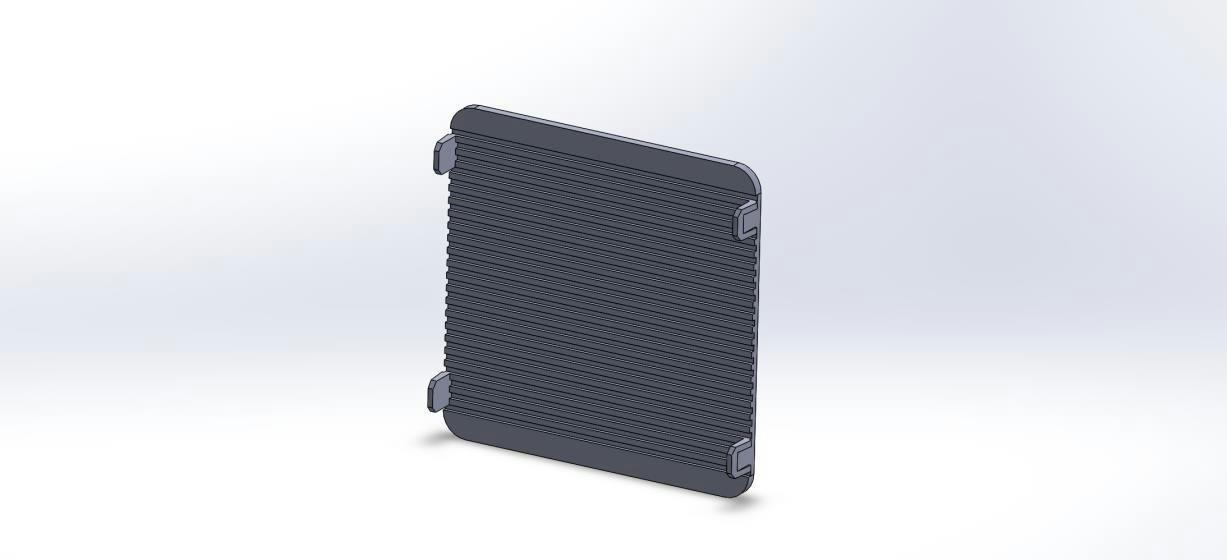
\includegraphics[width=441.9pt,height=201.65pt]{latexImage_c5cc85b5e65ab44f1c711223fc9a55ab.png}}
\end{picture}
\newpage
\begin{tikzpicture}[overlay]\path(0pt,0pt);\end{tikzpicture}
\begin{picture}(-5,0)(2.5,0)
\put(500.14,-727.616){\fontsize{12}{1}\usefont{T1}{ptm}{m}{n}\selectfont\color{color_29791}23}
\put(512.14,-727.616){\fontsize{12}{1}\usefont{T1}{ptm}{m}{n}\selectfont\color{color_29791} }
\put(515.14,-727.616){\fontsize{12}{1}\usefont{T1}{ptm}{m}{n}\selectfont\color{color_29791} }
\put(70.104,-742.496){\fontsize{10.56}{1}\usefont{T1}{ptm}{m}{n}\selectfont\color{color_29791} }
\put(72.744,-742.496){\fontsize{12}{1}\usefont{T1}{ptm}{m}{n}\selectfont\color{color_29791} }
\end{picture}
\begin{tikzpicture}[overlay]
\path(0pt,0pt);
\filldraw[color_270097][even odd rule]
(70.104pt, -77.38pt) -- (209.084pt, -77.38pt)
 -- (209.084pt, -77.38pt)
 -- (209.084pt, -60.91602pt)
 -- (209.084pt, -60.91602pt)
 -- (70.104pt, -60.91602pt) -- cycle
;
\filldraw[color_270097][even odd rule]
(209.57pt, -77.38pt) -- (511.06pt, -77.38pt)
 -- (511.06pt, -77.38pt)
 -- (511.06pt, -60.91602pt)
 -- (511.06pt, -60.91602pt)
 -- (209.57pt, -60.91602pt) -- cycle
;
\begin{scope}
\clip
(209.57pt, -77.38pt) -- (511.06pt, -77.38pt)
 -- (511.06pt, -77.38pt)
 -- (511.06pt, -63.07599pt)
 -- (511.06pt, -63.07599pt)
 -- (209.57pt, -63.07599pt) -- cycle
;
\filldraw[color_270097][even odd rule]
(214.73pt, -77.14001pt) -- (507.82pt, -77.14001pt)
 -- (507.82pt, -77.14001pt)
 -- (507.82pt, -63.07599pt)
 -- (507.82pt, -63.07599pt)
 -- (214.73pt, -63.07599pt) -- cycle
;
\begin{scope}
\clip
(209.57pt, -77.38pt) -- (511.06pt, -77.38pt)
 -- (511.06pt, -77.38pt)
 -- (511.06pt, -63.07599pt)
 -- (511.06pt, -63.07599pt)
 -- (209.57pt, -63.07599pt) -- cycle
;
\end{scope}
\end{scope}
\end{tikzpicture}
\begin{picture}(-5,0)(2.5,0)
\put(214.73,-72.58002){\fontsize{9.96}{1}\usefont{T1}{ptm}{m}{n}\selectfont\color{color_29791}改變一個}
\put(254.6796,-72.58002){\fontsize{9.96}{1}\usefont{T1}{ptm}{m}{n}\selectfont\color{color_29791}會影響}
\put(284.6691,-72.58002){\fontsize{9.96}{1}\usefont{T1}{ptm}{m}{n}\selectfont\color{color_29791}另一個}
\put(314.6587,-72.58002){\fontsize{9.96}{1}\usefont{T1}{ptm}{m}{n}\selectfont\color{color_29791}嗎?}
\put(334.63,-72.58002){\fontsize{9.96}{1}\usefont{T1}{ptm}{m}{n}\selectfont\color{color_29791} }
\put(337.03,-72.58002){\fontsize{12}{1}\usefont{T1}{ptm}{m}{n}\selectfont\color{color_29791} }
\end{picture}
\begin{tikzpicture}[overlay]
\path(0pt,0pt);
\filldraw[color_29791][even odd rule]
(209.09pt, -63.08002pt) -- (209.57pt, -63.08002pt)
 -- (209.57pt, -63.08002pt)
 -- (209.57pt, -60.92004pt)
 -- (209.57pt, -60.92004pt)
 -- (209.09pt, -60.92004pt) -- cycle
;
\filldraw[color_270097][even odd rule]
(209.09pt, -63.08002pt) -- (511.06pt, -63.08002pt)
 -- (511.06pt, -63.08002pt)
 -- (511.06pt, -60.92004pt)
 -- (511.06pt, -60.92004pt)
 -- (209.09pt, -60.92004pt) -- cycle
;
\filldraw[color_29791][even odd rule]
(209.09pt, -77.38pt) -- (209.57pt, -77.38pt)
 -- (209.57pt, -77.38pt)
 -- (209.57pt, -63.07599pt)
 -- (209.57pt, -63.07599pt)
 -- (209.09pt, -63.07599pt) -- cycle
;
\filldraw[color_270097][even odd rule]
(70.104pt, -126.94pt) -- (209.084pt, -126.94pt)
 -- (209.084pt, -126.94pt)
 -- (209.084pt, -77.85999pt)
 -- (209.084pt, -77.85999pt)
 -- (70.104pt, -77.85999pt) -- cycle
;
\begin{scope}
\clip
(70.104pt, -126.94pt) -- (209.084pt, -126.94pt)
 -- (209.084pt, -126.94pt)
 -- (209.084pt, -80.02002pt)
 -- (209.084pt, -80.02002pt)
 -- (70.104pt, -80.02002pt) -- cycle
;
\filldraw[color_270097][even odd rule]
(75.504pt, -94.06pt) -- (206.084pt, -94.06pt)
 -- (206.084pt, -94.06pt)
 -- (206.084pt, -80.02002pt)
 -- (206.084pt, -80.02002pt)
 -- (75.504pt, -80.02002pt) -- cycle
;
\begin{scope}
\clip
(70.104pt, -126.94pt) -- (209.084pt, -126.94pt)
 -- (209.084pt, -126.94pt)
 -- (209.084pt, -80.02002pt)
 -- (209.084pt, -80.02002pt)
 -- (70.104pt, -80.02002pt) -- cycle
;
\end{scope}
\end{scope}
\end{tikzpicture}
\begin{picture}(-5,0)(2.5,0)
\put(89.66,-89.5){\fontsize{9.96}{1}\usefont{T1}{ptm}{m}{n}\selectfont\color{color_29791}創}
\put(100.0881,-89.5){\fontsize{9.96}{1}\usefont{T1}{ptm}{m}{n}\selectfont\color{color_29791}建}
\put(110.3967,-89.5){\fontsize{9.96}{1}\usefont{T1}{ptm}{m}{n}\selectfont\color{color_29791}一}
\put(120.8248,-89.5){\fontsize{9.96}{1}\usefont{T1}{ptm}{m}{n}\selectfont\color{color_29791}個}
\put(131.1334,-89.5){\fontsize{9.96}{1}\usefont{T1}{ptm}{m}{n}\selectfont\color{color_29791}全}
\put(141.6811,-89.5){\fontsize{9.96}{1}\usefont{T1}{ptm}{m}{n}\selectfont\color{color_29791}新}
\put(152.1092,-89.5){\fontsize{9.96}{1}\usefont{T1}{ptm}{m}{n}\selectfont\color{color_29791}的}
\put(162.4178,-89.5){\fontsize{9.96}{1}\usefont{T1}{ptm}{m}{n}\selectfont\color{color_29791}生}
\put(172.9654,-89.5){\fontsize{9.96}{1}\usefont{T1}{ptm}{m}{n}\selectfont\color{color_29791}產}
\put(183.274,-89.5){\fontsize{9.96}{1}\usefont{T1}{ptm}{m}{n}\selectfont\color{color_29791}流}
\put(193.7021,-89.5){\fontsize{9.96}{1}\usefont{T1}{ptm}{m}{n}\selectfont\color{color_29791}程}
\end{picture}
\begin{tikzpicture}[overlay]
\path(0pt,0pt);
\begin{scope}
\clip
(70.104pt, -126.94pt) -- (209.084pt, -126.94pt)
 -- (209.084pt, -126.94pt)
 -- (209.084pt, -80.02002pt)
 -- (209.084pt, -80.02002pt)
 -- (70.104pt, -80.02002pt) -- cycle
;
\filldraw[color_270097][even odd rule]
(75.504pt, -108.1pt) -- (206.084pt, -108.1pt)
 -- (206.084pt, -108.1pt)
 -- (206.084pt, -94.06pt)
 -- (206.084pt, -94.06pt)
 -- (75.504pt, -94.06pt) -- cycle
;
\begin{scope}
\clip
(70.104pt, -126.94pt) -- (209.084pt, -126.94pt)
 -- (209.084pt, -126.94pt)
 -- (209.084pt, -80.02002pt)
 -- (209.084pt, -80.02002pt)
 -- (70.104pt, -80.02002pt) -- cycle
;
\end{scope}
\end{scope}
\end{tikzpicture}
\begin{picture}(-5,0)(2.5,0)
\put(75.504,-103.54){\fontsize{9.96}{1}\usefont{T1}{ptm}{m}{n}\selectfont\color{color_29791}有多容易}
\put(115.4536,-103.54){\fontsize{9.96}{1}\usefont{T1}{ptm}{m}{n}\selectfont\color{color_29791}?}
\put(125.42,-103.54){\fontsize{9.96}{1}\usefont{T1}{ptm}{m}{n}\selectfont\color{color_29791} }
\put(127.82,-103.54){\fontsize{12}{1}\usefont{T1}{ptm}{m}{n}\selectfont\color{color_29791} }
\put(214.73,-89.5){\fontsize{9.96}{1}\usefont{T1}{ptm}{m}{n}\selectfont\color{color_29791}如何描述}
\put(254.6796,-89.5){\fontsize{9.96}{1}\usefont{T1}{ptm}{m}{n}\selectfont\color{color_29791}該過程}
\put(284.6691,-89.5){\fontsize{9.96}{1}\usefont{T1}{ptm}{m}{n}\selectfont\color{color_29791}?}
\put(294.65,-89.5){\fontsize{9.96}{1}\usefont{T1}{ptm}{m}{n}\selectfont\color{color_29791} }
\put(297.05,-89.5){\fontsize{12}{1}\usefont{T1}{ptm}{m}{n}\selectfont\color{color_29791} }
\end{picture}
\begin{tikzpicture}[overlay]
\path(0pt,0pt);
\filldraw[color_29791][even odd rule]
(70.104pt, -77.85999pt) -- (209.084pt, -77.85999pt)
 -- (209.084pt, -77.85999pt)
 -- (209.084pt, -77.38pt)
 -- (209.084pt, -77.38pt)
 -- (70.104pt, -77.38pt) -- cycle
;
\filldraw[color_270097][even odd rule]
(70.104pt, -80.02002pt) -- (209.084pt, -80.02002pt)
 -- (209.084pt, -80.02002pt)
 -- (209.084pt, -77.86005pt)
 -- (209.084pt, -77.86005pt)
 -- (70.104pt, -77.86005pt) -- cycle
;
\filldraw[color_29791][even odd rule]
(209.09pt, -80.02002pt) -- (209.57pt, -80.02002pt)
 -- (209.57pt, -80.02002pt)
 -- (209.57pt, -77.38pt)
 -- (209.57pt, -77.38pt)
 -- (209.09pt, -77.38pt) -- cycle
;
\filldraw[color_29791][even odd rule]
(209.57pt, -77.85999pt) -- (511.06pt, -77.85999pt)
 -- (511.06pt, -77.85999pt)
 -- (511.06pt, -77.38pt)
 -- (511.06pt, -77.38pt)
 -- (209.57pt, -77.38pt) -- cycle
;
\filldraw[color_29791][even odd rule]
(209.09pt, -94.29999pt) -- (209.57pt, -94.29999pt)
 -- (209.57pt, -94.29999pt)
 -- (209.57pt, -80.01996pt)
 -- (209.57pt, -80.01996pt)
 -- (209.09pt, -80.01996pt) -- cycle
;
\filldraw[color_270097][even odd rule]
(209.57pt, -110.5pt) -- (511.06pt, -110.5pt)
 -- (511.06pt, -110.5pt)
 -- (511.06pt, -94.29999pt)
 -- (511.06pt, -94.29999pt)
 -- (209.57pt, -94.29999pt) -- cycle
;
\begin{scope}
\clip
(209.57pt, -110.5pt) -- (511.06pt, -110.5pt)
 -- (511.06pt, -110.5pt)
 -- (511.06pt, -96.46002pt)
 -- (511.06pt, -96.46002pt)
 -- (209.57pt, -96.46002pt) -- cycle
;
\filldraw[color_270097][even odd rule]
(214.73pt, -110.5pt) -- (507.82pt, -110.5pt)
 -- (507.82pt, -110.5pt)
 -- (507.82pt, -96.46002pt)
 -- (507.82pt, -96.46002pt)
 -- (214.73pt, -96.46002pt) -- cycle
;
\begin{scope}
\clip
(209.57pt, -110.5pt) -- (511.06pt, -110.5pt)
 -- (511.06pt, -110.5pt)
 -- (511.06pt, -96.46002pt)
 -- (511.06pt, -96.46002pt)
 -- (209.57pt, -96.46002pt) -- cycle
;
\end{scope}
\end{scope}
\end{tikzpicture}
\begin{picture}(-5,0)(2.5,0)
\put(214.73,-105.94){\fontsize{9.96}{1}\usefont{T1}{ptm}{m}{n}\selectfont\color{color_29791}該過程如}
\put(254.6796,-105.94){\fontsize{9.96}{1}\usefont{T1}{ptm}{m}{n}\selectfont\color{color_29791}何集成}
\put(284.6691,-105.94){\fontsize{9.96}{1}\usefont{T1}{ptm}{m}{n}\selectfont\color{color_29791}和引用}
\put(314.6587,-105.94){\fontsize{9.96}{1}\usefont{T1}{ptm}{m}{n}\selectfont\color{color_29791}其生}
\put(334.6883,-105.94){\fontsize{9.96}{1}\usefont{T1}{ptm}{m}{n}\selectfont\color{color_29791}產的產品}
\put(374.6378,-105.94){\fontsize{9.96}{1}\usefont{T1}{ptm}{m}{n}\selectfont\color{color_29791}?}
\put(384.67,-105.94){\fontsize{9.96}{1}\usefont{T1}{ptm}{m}{n}\selectfont\color{color_29791} }
\put(387.07,-105.94){\fontsize{12}{1}\usefont{T1}{ptm}{m}{n}\selectfont\color{color_29791} }
\end{picture}
\begin{tikzpicture}[overlay]
\path(0pt,0pt);
\filldraw[color_29791][even odd rule]
(209.09pt, -96.46002pt) -- (209.57pt, -96.46002pt)
 -- (209.57pt, -96.46002pt)
 -- (209.57pt, -94.30005pt)
 -- (209.57pt, -94.30005pt)
 -- (209.09pt, -94.30005pt) -- cycle
;
\filldraw[color_270097][even odd rule]
(209.57pt, -96.46002pt) -- (511.06pt, -96.46002pt)
 -- (511.06pt, -96.46002pt)
 -- (511.06pt, -94.30005pt)
 -- (511.06pt, -94.30005pt)
 -- (209.57pt, -94.30005pt) -- cycle
;
\filldraw[color_29791][even odd rule]
(209.09pt, -110.5pt) -- (209.57pt, -110.5pt)
 -- (209.57pt, -110.5pt)
 -- (209.57pt, -96.46002pt)
 -- (209.57pt, -96.46002pt)
 -- (209.09pt, -96.46002pt) -- cycle
;
\filldraw[color_283006][even odd rule]
(209.57pt, -126.94pt) -- (511.06pt, -126.94pt)
 -- (511.06pt, -126.94pt)
 -- (511.06pt, -110.5pt)
 -- (511.06pt, -110.5pt)
 -- (209.57pt, -110.5pt) -- cycle
;
\begin{scope}
\clip
(209.57pt, -126.94pt) -- (511.06pt, -126.94pt)
 -- (511.06pt, -126.94pt)
 -- (511.06pt, -112.66pt)
 -- (511.06pt, -112.66pt)
 -- (209.57pt, -112.66pt) -- cycle
;
\filldraw[color_283006][even odd rule]
(214.73pt, -126.7pt) -- (507.82pt, -126.7pt)
 -- (507.82pt, -126.7pt)
 -- (507.82pt, -112.66pt)
 -- (507.82pt, -112.66pt)
 -- (214.73pt, -112.66pt) -- cycle
;
\begin{scope}
\clip
(209.57pt, -126.94pt) -- (511.06pt, -126.94pt)
 -- (511.06pt, -126.94pt)
 -- (511.06pt, -112.66pt)
 -- (511.06pt, -112.66pt)
 -- (209.57pt, -112.66pt) -- cycle
;
\end{scope}
\end{scope}
\end{tikzpicture}
\begin{picture}(-5,0)(2.5,0)
\put(214.73,-122.14){\fontsize{9.96}{1}\usefont{T1}{ptm}{m}{n}\selectfont\color{color_29791}改變一個}
\put(254.6796,-122.14){\fontsize{9.96}{1}\usefont{T1}{ptm}{m}{n}\selectfont\color{color_29791}會影響}
\put(284.6691,-122.14){\fontsize{9.96}{1}\usefont{T1}{ptm}{m}{n}\selectfont\color{color_29791}另一個}
\put(314.6587,-122.14){\fontsize{9.96}{1}\usefont{T1}{ptm}{m}{n}\selectfont\color{color_29791}嗎?}
\put(334.63,-122.14){\fontsize{9.96}{1}\usefont{T1}{ptm}{m}{n}\selectfont\color{color_29791} }
\put(337.03,-122.14){\fontsize{12}{1}\usefont{T1}{ptm}{m}{n}\selectfont\color{color_29791} }
\end{picture}
\begin{tikzpicture}[overlay]
\path(0pt,0pt);
\filldraw[color_29791][even odd rule]
(209.09pt, -112.66pt) -- (209.57pt, -112.66pt)
 -- (209.57pt, -112.66pt)
 -- (209.57pt, -110.5pt)
 -- (209.57pt, -110.5pt)
 -- (209.09pt, -110.5pt) -- cycle
;
\filldraw[color_283006][even odd rule]
(209.57pt, -112.66pt) -- (511.06pt, -112.66pt)
 -- (511.06pt, -112.66pt)
 -- (511.06pt, -110.5pt)
 -- (511.06pt, -110.5pt)
 -- (209.57pt, -110.5pt) -- cycle
;
\filldraw[color_29791][even odd rule]
(209.09pt, -126.94pt) -- (209.57pt, -126.94pt)
 -- (209.57pt, -126.94pt)
 -- (209.57pt, -112.66pt)
 -- (209.57pt, -112.66pt)
 -- (209.09pt, -112.66pt) -- cycle
;
\filldraw[color_270097][even odd rule]
(70.104pt, -176.62pt) -- (209.084pt, -176.62pt)
 -- (209.084pt, -176.62pt)
 -- (209.084pt, -127.42pt)
 -- (209.084pt, -127.42pt)
 -- (70.104pt, -127.42pt) -- cycle
;
\begin{scope}
\clip
(70.104pt, -176.62pt) -- (209.084pt, -176.62pt)
 -- (209.084pt, -176.62pt)
 -- (209.084pt, -129.58pt)
 -- (209.084pt, -129.58pt)
 -- (70.104pt, -129.58pt) -- cycle
;
\filldraw[color_270097][even odd rule]
(75.504pt, -144.7pt) -- (206.084pt, -144.7pt)
 -- (206.084pt, -144.7pt)
 -- (206.084pt, -129.58pt)
 -- (206.084pt, -129.58pt)
 -- (75.504pt, -129.58pt) -- cycle
;
\begin{scope}
\clip
(70.104pt, -176.62pt) -- (209.084pt, -176.62pt)
 -- (209.084pt, -176.62pt)
 -- (209.084pt, -129.58pt)
 -- (209.084pt, -129.58pt)
 -- (70.104pt, -129.58pt) -- cycle
;
\end{scope}
\end{scope}
\end{tikzpicture}
\begin{picture}(-5,0)(2.5,0)
\put(89.66,-139.18){\fontsize{9.96}{1}\usefont{T1}{ptm}{m}{n}\selectfont\color{color_29791}改進現有}
\put(129.6096,-139.18){\fontsize{9.96}{1}\usefont{T1}{ptm}{m}{n}\selectfont\color{color_29791}產品的}
\put(159.5991,-139.18){\fontsize{9.96}{1}\usefont{T1}{ptm}{m}{n}\selectfont\color{color_29791}難易程}
\put(189.5887,-139.18){\fontsize{9.96}{1}\usefont{T1}{ptm}{m}{n}\selectfont\color{color_29791}度}
\put(199.61,-139.18){\fontsize{9.96}{1}\usefont{T1}{ptm}{m}{n}\selectfont\color{color_29791}  }
\put(204.17,-139.18){\fontsize{12}{1}\usefont{T1}{ptm}{m}{n}\selectfont\color{color_29791} }
\end{picture}
\begin{tikzpicture}[overlay]
\path(0pt,0pt);
\begin{scope}
\clip
(70.104pt, -176.62pt) -- (209.084pt, -176.62pt)
 -- (209.084pt, -176.62pt)
 -- (209.084pt, -129.58pt)
 -- (209.084pt, -129.58pt)
 -- (70.104pt, -129.58pt) -- cycle
;
\filldraw[color_270097][even odd rule]
(75.504pt, -159.58pt) -- (206.084pt, -159.58pt)
 -- (206.084pt, -159.58pt)
 -- (206.084pt, -144.7pt)
 -- (206.084pt, -144.7pt)
 -- (75.504pt, -144.7pt) -- cycle
;
\begin{scope}
\clip
(70.104pt, -176.62pt) -- (209.084pt, -176.62pt)
 -- (209.084pt, -176.62pt)
 -- (209.084pt, -129.58pt)
 -- (209.084pt, -129.58pt)
 -- (70.104pt, -129.58pt) -- cycle
;
\end{scope}
\end{scope}
\end{tikzpicture}
\begin{picture}(-5,0)(2.5,0)
\put(75.504,-155.86){\fontsize{9.96}{1}\usefont{T1}{ptm}{m}{n}\selectfont\color{color_29791} }
\put(77.784,-155.86){\fontsize{12}{1}\usefont{T1}{ptm}{m}{n}\selectfont\color{color_29791} }
\end{picture}
\begin{tikzpicture}[overlay]
\path(0pt,0pt);
\filldraw[color_270097][even odd rule]
(209.57pt, -143.86pt) -- (511.06pt, -143.86pt)
 -- (511.06pt, -143.86pt)
 -- (511.06pt, -127.42pt)
 -- (511.06pt, -127.42pt)
 -- (209.57pt, -127.42pt) -- cycle
;
\begin{scope}
\clip
(209.57pt, -143.86pt) -- (511.06pt, -143.86pt)
 -- (511.06pt, -143.86pt)
 -- (511.06pt, -129.58pt)
 -- (511.06pt, -129.58pt)
 -- (209.57pt, -129.58pt) -- cycle
;
\filldraw[color_270097][even odd rule]
(214.73pt, -143.62pt) -- (507.82pt, -143.62pt)
 -- (507.82pt, -143.62pt)
 -- (507.82pt, -129.58pt)
 -- (507.82pt, -129.58pt)
 -- (214.73pt, -129.58pt) -- cycle
;
\begin{scope}
\clip
(209.57pt, -143.86pt) -- (511.06pt, -143.86pt)
 -- (511.06pt, -143.86pt)
 -- (511.06pt, -129.58pt)
 -- (511.06pt, -129.58pt)
 -- (209.57pt, -129.58pt) -- cycle
;
\end{scope}
\end{scope}
\end{tikzpicture}
\begin{picture}(-5,0)(2.5,0)
\put(214.73,-139.06){\fontsize{9.96}{1}\usefont{T1}{ptm}{m}{n}\selectfont\color{color_29791}更新其元}
\put(254.6796,-139.06){\fontsize{9.96}{1}\usefont{T1}{ptm}{m}{n}\selectfont\color{color_29791}數據是}
\put(284.6691,-139.06){\fontsize{9.96}{1}\usefont{T1}{ptm}{m}{n}\selectfont\color{color_29791}多麼容}
\put(314.6587,-139.06){\fontsize{9.96}{1}\usefont{T1}{ptm}{m}{n}\selectfont\color{color_29791}易}
\put(324.67,-139.06){\fontsize{9.96}{1}\usefont{T1}{ptm}{m}{n}\selectfont\color{color_29791} }
\put(327.07,-139.06){\fontsize{12}{1}\usefont{T1}{ptm}{m}{n}\selectfont\color{color_29791} }
\end{picture}
\begin{tikzpicture}[overlay]
\path(0pt,0pt);
\filldraw[color_29791][even odd rule]
(70.104pt, -127.42pt) -- (209.084pt, -127.42pt)
 -- (209.084pt, -127.42pt)
 -- (209.084pt, -126.94pt)
 -- (209.084pt, -126.94pt)
 -- (70.104pt, -126.94pt) -- cycle
;
\filldraw[color_270097][even odd rule]
(70.104pt, -129.58pt) -- (209.084pt, -129.58pt)
 -- (209.084pt, -129.58pt)
 -- (209.084pt, -127.42pt)
 -- (209.084pt, -127.42pt)
 -- (70.104pt, -127.42pt) -- cycle
;
\filldraw[color_29791][even odd rule]
(209.09pt, -129.58pt) -- (209.57pt, -129.58pt)
 -- (209.57pt, -129.58pt)
 -- (209.57pt, -126.94pt)
 -- (209.57pt, -126.94pt)
 -- (209.09pt, -126.94pt) -- cycle
;
\filldraw[color_29791][even odd rule]
(209.57pt, -127.42pt) -- (511.06pt, -127.42pt)
 -- (511.06pt, -127.42pt)
 -- (511.06pt, -126.94pt)
 -- (511.06pt, -126.94pt)
 -- (209.57pt, -126.94pt) -- cycle
;
\filldraw[color_270097][even odd rule]
(209.57pt, -129.58pt) -- (511.06pt, -129.58pt)
 -- (511.06pt, -129.58pt)
 -- (511.06pt, -127.42pt)
 -- (511.06pt, -127.42pt)
 -- (209.57pt, -127.42pt) -- cycle
;
\filldraw[color_29791][even odd rule]
(209.09pt, -143.86pt) -- (209.57pt, -143.86pt)
 -- (209.57pt, -143.86pt)
 -- (209.57pt, -129.58pt)
 -- (209.57pt, -129.58pt)
 -- (209.09pt, -129.58pt) -- cycle
;
\begin{scope}
\clip
(209.57pt, -160.06pt) -- (511.06pt, -160.06pt)
 -- (511.06pt, -160.06pt)
 -- (511.06pt, -146.02pt)
 -- (511.06pt, -146.02pt)
 -- (209.57pt, -146.02pt) -- cycle
;
\begin{scope}
\clip
(209.57pt, -160.06pt) -- (511.06pt, -160.06pt)
 -- (511.06pt, -160.06pt)
 -- (511.06pt, -146.02pt)
 -- (511.06pt, -146.02pt)
 -- (209.57pt, -146.02pt) -- cycle
;
\end{scope}
\end{scope}
\end{tikzpicture}
\begin{picture}(-5,0)(2.5,0)
\put(214.73,-155.5){\fontsize{9.96}{1}\usefont{T1}{ptm}{m}{n}\selectfont\color{color_29791}確定更改}
\put(254.6796,-155.5){\fontsize{9.96}{1}\usefont{T1}{ptm}{m}{n}\selectfont\color{color_29791}的影響}
\put(284.6691,-155.5){\fontsize{9.96}{1}\usefont{T1}{ptm}{m}{n}\selectfont\color{color_29791}是多麼}
\put(314.6587,-155.5){\fontsize{9.96}{1}\usefont{T1}{ptm}{m}{n}\selectfont\color{color_29791}容易}
\put(334.63,-155.5){\fontsize{9.96}{1}\usefont{T1}{ptm}{m}{n}\selectfont\color{color_29791} }
\put(337.03,-155.5){\fontsize{12}{1}\usefont{T1}{ptm}{m}{n}\selectfont\color{color_29791} }
\end{picture}
\begin{tikzpicture}[overlay]
\path(0pt,0pt);
\filldraw[color_29791][even odd rule]
(209.09pt, -146.02pt) -- (209.57pt, -146.02pt)
 -- (209.57pt, -146.02pt)
 -- (209.57pt, -143.86pt)
 -- (209.57pt, -143.86pt)
 -- (209.09pt, -143.86pt) -- cycle
;
\filldraw[color_29791][even odd rule]
(209.09pt, -160.06pt) -- (209.57pt, -160.06pt)
 -- (209.57pt, -160.06pt)
 -- (209.57pt, -146.02pt)
 -- (209.57pt, -146.02pt)
 -- (209.09pt, -146.02pt) -- cycle
;
\filldraw[color_270097][even odd rule]
(209.57pt, -176.62pt) -- (511.06pt, -176.62pt)
 -- (511.06pt, -176.62pt)
 -- (511.06pt, -160.06pt)
 -- (511.06pt, -160.06pt)
 -- (209.57pt, -160.06pt) -- cycle
;
\begin{scope}
\clip
(209.57pt, -176.62pt) -- (511.06pt, -176.62pt)
 -- (511.06pt, -176.62pt)
 -- (511.06pt, -162.22pt)
 -- (511.06pt, -162.22pt)
 -- (209.57pt, -162.22pt) -- cycle
;
\filldraw[color_270097][even odd rule]
(214.73pt, -176.26pt) -- (507.82pt, -176.26pt)
 -- (507.82pt, -176.26pt)
 -- (507.82pt, -162.22pt)
 -- (507.82pt, -162.22pt)
 -- (214.73pt, -162.22pt) -- cycle
;
\begin{scope}
\clip
(209.57pt, -176.62pt) -- (511.06pt, -176.62pt)
 -- (511.06pt, -176.62pt)
 -- (511.06pt, -162.22pt)
 -- (511.06pt, -162.22pt)
 -- (209.57pt, -162.22pt) -- cycle
;
\end{scope}
\end{scope}
\end{tikzpicture}
\begin{picture}(-5,0)(2.5,0)
\put(214.73,-171.7){\fontsize{9.96}{1}\usefont{T1}{ptm}{m}{n}\selectfont\color{color_29791}該軟體如}
\put(254.6796,-171.7){\fontsize{9.96}{1}\usefont{T1}{ptm}{m}{n}\selectfont\color{color_29791}何處理}
\put(284.6691,-171.7){\fontsize{9.96}{1}\usefont{T1}{ptm}{m}{n}\selectfont\color{color_29791}不同的}
\put(314.6587,-171.7){\fontsize{9.96}{1}\usefont{T1}{ptm}{m}{n}\selectfont\color{color_29791}產品}
\put(334.6883,-171.7){\fontsize{9.96}{1}\usefont{T1}{ptm}{m}{n}\selectfont\color{color_29791}修訂版?}
\put(374.59,-171.7){\fontsize{9.96}{1}\usefont{T1}{ptm}{m}{n}\selectfont\color{color_29791} }
\put(376.99,-171.7){\fontsize{12}{1}\usefont{T1}{ptm}{m}{n}\selectfont\color{color_29791} }
\end{picture}
\begin{tikzpicture}[overlay]
\path(0pt,0pt);
\filldraw[color_29791][even odd rule]
(209.09pt, -162.22pt) -- (209.57pt, -162.22pt)
 -- (209.57pt, -162.22pt)
 -- (209.57pt, -160.06pt)
 -- (209.57pt, -160.06pt)
 -- (209.09pt, -160.06pt) -- cycle
;
\filldraw[color_270097][even odd rule]
(209.57pt, -162.22pt) -- (511.06pt, -162.22pt)
 -- (511.06pt, -162.22pt)
 -- (511.06pt, -160.06pt)
 -- (511.06pt, -160.06pt)
 -- (209.57pt, -160.06pt) -- cycle
;
\filldraw[color_29791][even odd rule]
(209.09pt, -176.62pt) -- (209.57pt, -176.62pt)
 -- (209.57pt, -176.62pt)
 -- (209.57pt, -162.22pt)
 -- (209.57pt, -162.22pt)
 -- (209.09pt, -162.22pt) -- cycle
;
\filldraw[color_270097][even odd rule]
(70.104pt, -240.22pt) -- (209.084pt, -240.22pt)
 -- (209.084pt, -240.22pt)
 -- (209.084pt, -177.1pt)
 -- (209.084pt, -177.1pt)
 -- (70.104pt, -177.1pt) -- cycle
;
\begin{scope}
\clip
(70.104pt, -240.22pt) -- (209.084pt, -240.22pt)
 -- (209.084pt, -240.22pt)
 -- (209.084pt, -179.2599pt)
 -- (209.084pt, -179.2599pt)
 -- (70.104pt, -179.2599pt) -- cycle
;
\filldraw[color_270097][even odd rule]
(75.504pt, -193.3pt) -- (206.084pt, -193.3pt)
 -- (206.084pt, -193.3pt)
 -- (206.084pt, -179.26pt)
 -- (206.084pt, -179.26pt)
 -- (75.504pt, -179.26pt) -- cycle
;
\begin{scope}
\clip
(70.104pt, -240.22pt) -- (209.084pt, -240.22pt)
 -- (209.084pt, -240.22pt)
 -- (209.084pt, -179.2599pt)
 -- (209.084pt, -179.2599pt)
 -- (70.104pt, -179.2599pt) -- cycle
;
\end{scope}
\end{scope}
\end{tikzpicture}
\begin{picture}(-5,0)(2.5,0)
\put(75.504,-188.74){\fontsize{9.96}{1}\usefont{T1}{ptm}{m}{n}\selectfont\color{color_29791}改進現有}
\put(115.4536,-188.74){\fontsize{9.96}{1}\usefont{T1}{ptm}{m}{n}\selectfont\color{color_29791}生產流}
\put(145.4431,-188.74){\fontsize{9.96}{1}\usefont{T1}{ptm}{m}{n}\selectfont\color{color_29791}程是多}
\put(175.4327,-188.74){\fontsize{9.96}{1}\usefont{T1}{ptm}{m}{n}\selectfont\color{color_29791}麼容}
\put(195.4622,-188.74){\fontsize{9.96}{1}\usefont{T1}{ptm}{m}{n}\selectfont\color{color_29791}易}
\put(205.49,-188.74){\fontsize{9.96}{1}\usefont{T1}{ptm}{m}{n}\selectfont\color{color_29791} }
\put(207.77,-188.74){\fontsize{12}{1}\usefont{T1}{ptm}{m}{n}\selectfont\color{color_29791} }
\put(214.73,-188.74){\fontsize{9.96}{1}\usefont{T1}{ptm}{m}{n}\selectfont\color{color_29791}更新其元}
\put(254.6796,-188.74){\fontsize{9.96}{1}\usefont{T1}{ptm}{m}{n}\selectfont\color{color_29791}數據是}
\put(284.6691,-188.74){\fontsize{9.96}{1}\usefont{T1}{ptm}{m}{n}\selectfont\color{color_29791}多麼容}
\put(314.6587,-188.74){\fontsize{9.96}{1}\usefont{T1}{ptm}{m}{n}\selectfont\color{color_29791}易}
\put(324.67,-188.74){\fontsize{9.96}{1}\usefont{T1}{ptm}{m}{n}\selectfont\color{color_29791}  }
\put(329.23,-188.74){\fontsize{12}{1}\usefont{T1}{ptm}{m}{n}\selectfont\color{color_29791} }
\end{picture}
\begin{tikzpicture}[overlay]
\path(0pt,0pt);
\filldraw[color_29791][even odd rule]
(70.104pt, -177.1pt) -- (209.084pt, -177.1pt)
 -- (209.084pt, -177.1pt)
 -- (209.084pt, -176.62pt)
 -- (209.084pt, -176.62pt)
 -- (70.104pt, -176.62pt) -- cycle
;
\filldraw[color_270097][even odd rule]
(70.104pt, -179.26pt) -- (209.084pt, -179.26pt)
 -- (209.084pt, -179.26pt)
 -- (209.084pt, -177.1pt)
 -- (209.084pt, -177.1pt)
 -- (70.104pt, -177.1pt) -- cycle
;
\filldraw[color_29791][even odd rule]
(209.09pt, -179.26pt) -- (209.57pt, -179.26pt)
 -- (209.57pt, -179.26pt)
 -- (209.57pt, -176.62pt)
 -- (209.57pt, -176.62pt)
 -- (209.09pt, -176.62pt) -- cycle
;
\filldraw[color_29791][even odd rule]
(209.57pt, -177.1pt) -- (511.06pt, -177.1pt)
 -- (511.06pt, -177.1pt)
 -- (511.06pt, -176.62pt)
 -- (511.06pt, -176.62pt)
 -- (209.57pt, -176.62pt) -- cycle
;
\filldraw[color_29791][even odd rule]
(209.09pt, -193.54pt) -- (209.57pt, -193.54pt)
 -- (209.57pt, -193.54pt)
 -- (209.57pt, -179.2599pt)
 -- (209.57pt, -179.2599pt)
 -- (209.09pt, -179.2599pt) -- cycle
;
\filldraw[color_270097][even odd rule]
(209.57pt, -209.74pt) -- (511.06pt, -209.74pt)
 -- (511.06pt, -209.74pt)
 -- (511.06pt, -193.54pt)
 -- (511.06pt, -193.54pt)
 -- (209.57pt, -193.54pt) -- cycle
;
\begin{scope}
\clip
(209.57pt, -209.74pt) -- (511.06pt, -209.74pt)
 -- (511.06pt, -209.74pt)
 -- (511.06pt, -195.7pt)
 -- (511.06pt, -195.7pt)
 -- (209.57pt, -195.7pt) -- cycle
;
\filldraw[color_270097][even odd rule]
(214.73pt, -209.74pt) -- (507.82pt, -209.74pt)
 -- (507.82pt, -209.74pt)
 -- (507.82pt, -195.7pt)
 -- (507.82pt, -195.7pt)
 -- (214.73pt, -195.7pt) -- cycle
;
\begin{scope}
\clip
(209.57pt, -209.74pt) -- (511.06pt, -209.74pt)
 -- (511.06pt, -209.74pt)
 -- (511.06pt, -195.7pt)
 -- (511.06pt, -195.7pt)
 -- (209.57pt, -195.7pt) -- cycle
;
\end{scope}
\end{scope}
\end{tikzpicture}
\begin{picture}(-5,0)(2.5,0)
\put(214.73,-205.18){\fontsize{9.96}{1}\usefont{T1}{ptm}{m}{n}\selectfont\color{color_29791}確定更改}
\put(254.6796,-205.18){\fontsize{9.96}{1}\usefont{T1}{ptm}{m}{n}\selectfont\color{color_29791}的影響}
\put(284.6691,-205.18){\fontsize{9.96}{1}\usefont{T1}{ptm}{m}{n}\selectfont\color{color_29791}是多麼}
\put(314.6587,-205.18){\fontsize{9.96}{1}\usefont{T1}{ptm}{m}{n}\selectfont\color{color_29791}容易}
\put(334.63,-205.18){\fontsize{9.96}{1}\usefont{T1}{ptm}{m}{n}\selectfont\color{color_29791} }
\put(337.03,-205.18){\fontsize{12}{1}\usefont{T1}{ptm}{m}{n}\selectfont\color{color_29791} }
\end{picture}
\begin{tikzpicture}[overlay]
\path(0pt,0pt);
\filldraw[color_29791][even odd rule]
(209.09pt, -195.7pt) -- (209.57pt, -195.7pt)
 -- (209.57pt, -195.7pt)
 -- (209.57pt, -193.54pt)
 -- (209.57pt, -193.54pt)
 -- (209.09pt, -193.54pt) -- cycle
;
\filldraw[color_270097][even odd rule]
(209.57pt, -195.7pt) -- (511.06pt, -195.7pt)
 -- (511.06pt, -195.7pt)
 -- (511.06pt, -193.54pt)
 -- (511.06pt, -193.54pt)
 -- (209.57pt, -193.54pt) -- cycle
;
\filldraw[color_29791][even odd rule]
(209.09pt, -209.74pt) -- (209.57pt, -209.74pt)
 -- (209.57pt, -209.74pt)
 -- (209.57pt, -195.7pt)
 -- (209.57pt, -195.7pt)
 -- (209.09pt, -195.7pt) -- cycle
;
\begin{scope}
\clip
(209.57pt, -240.22pt) -- (511.06pt, -240.22pt)
 -- (511.06pt, -240.22pt)
 -- (511.06pt, -211.9pt)
 -- (511.06pt, -211.9pt)
 -- (209.57pt, -211.9pt) -- cycle
;
\begin{scope}
\clip
(209.57pt, -240.22pt) -- (511.06pt, -240.22pt)
 -- (511.06pt, -240.22pt)
 -- (511.06pt, -211.9pt)
 -- (511.06pt, -211.9pt)
 -- (209.57pt, -211.9pt) -- cycle
;
\end{scope}
\end{scope}
\end{tikzpicture}
\begin{picture}(-5,0)(2.5,0)
\put(214.73,-221.38){\fontsize{9.96}{1}\usefont{T1}{ptm}{m}{n}\selectfont\color{color_29791}該軟體如}
\put(254.6796,-221.38){\fontsize{9.96}{1}\usefont{T1}{ptm}{m}{n}\selectfont\color{color_29791}何處理}
\put(284.6691,-221.38){\fontsize{9.96}{1}\usefont{T1}{ptm}{m}{n}\selectfont\color{color_29791}不同的}
\put(314.6587,-221.38){\fontsize{9.96}{1}\usefont{T1}{ptm}{m}{n}\selectfont\color{color_29791}生產}
\put(334.6883,-221.38){\fontsize{9.96}{1}\usefont{T1}{ptm}{m}{n}\selectfont\color{color_29791}過程修訂}
\put(374.6378,-221.38){\fontsize{9.96}{1}\usefont{T1}{ptm}{m}{n}\selectfont\color{color_29791}?}
\put(384.67,-221.38){\fontsize{9.96}{1}\usefont{T1}{ptm}{m}{n}\selectfont\color{color_29791} }
\put(387.07,-221.38){\fontsize{12}{1}\usefont{T1}{ptm}{m}{n}\selectfont\color{color_29791} }
\end{picture}
\begin{tikzpicture}[overlay]
\path(0pt,0pt);
\filldraw[color_29791][even odd rule]
(209.09pt, -211.9pt) -- (209.57pt, -211.9pt)
 -- (209.57pt, -211.9pt)
 -- (209.57pt, -209.7401pt)
 -- (209.57pt, -209.7401pt)
 -- (209.09pt, -209.7401pt) -- cycle
;
\filldraw[color_29791][even odd rule]
(209.09pt, -240.22pt) -- (209.57pt, -240.22pt)
 -- (209.57pt, -240.22pt)
 -- (209.57pt, -211.9pt)
 -- (209.57pt, -211.9pt)
 -- (209.09pt, -211.9pt) -- cycle
;
\filldraw[color_270097][even odd rule]
(70.104pt, -303.61pt) -- (209.084pt, -303.61pt)
 -- (209.084pt, -303.61pt)
 -- (209.084pt, -240.706pt)
 -- (209.084pt, -240.706pt)
 -- (70.104pt, -240.706pt) -- cycle
;
\begin{scope}
\clip
(70.104pt, -303.61pt) -- (209.084pt, -303.61pt)
 -- (209.084pt, -303.61pt)
 -- (209.084pt, -242.866pt)
 -- (209.084pt, -242.866pt)
 -- (70.104pt, -242.866pt) -- cycle
;
\filldraw[color_270097][even odd rule]
(75.504pt, -256.93pt) -- (206.084pt, -256.93pt)
 -- (206.084pt, -256.93pt)
 -- (206.084pt, -242.866pt)
 -- (206.084pt, -242.866pt)
 -- (75.504pt, -242.866pt) -- cycle
;
\begin{scope}
\clip
(70.104pt, -303.61pt) -- (209.084pt, -303.61pt)
 -- (209.084pt, -303.61pt)
 -- (209.084pt, -242.866pt)
 -- (209.084pt, -242.866pt)
 -- (70.104pt, -242.866pt) -- cycle
;
\end{scope}
\end{scope}
\end{tikzpicture}
\begin{picture}(-5,0)(2.5,0)
\put(75.504,-252.37){\fontsize{9.96}{1}\usefont{T1}{ptm}{m}{n}\selectfont\color{color_29791}查找與產}
\put(115.4536,-252.37){\fontsize{9.96}{1}\usefont{T1}{ptm}{m}{n}\selectfont\color{color_29791}品或流}
\put(145.4431,-252.37){\fontsize{9.96}{1}\usefont{T1}{ptm}{m}{n}\selectfont\color{color_29791}程相關}
\put(175.4327,-252.37){\fontsize{9.96}{1}\usefont{T1}{ptm}{m}{n}\selectfont\color{color_29791}的數}
\put(195.4622,-252.37){\fontsize{9.96}{1}\usefont{T1}{ptm}{m}{n}\selectfont\color{color_29791}據}
\end{picture}
\begin{tikzpicture}[overlay]
\path(0pt,0pt);
\begin{scope}
\clip
(70.104pt, -303.61pt) -- (209.084pt, -303.61pt)
 -- (209.084pt, -303.61pt)
 -- (209.084pt, -242.866pt)
 -- (209.084pt, -242.866pt)
 -- (70.104pt, -242.866pt) -- cycle
;
\filldraw[color_270097][even odd rule]
(75.504pt, -270.97pt) -- (206.084pt, -270.97pt)
 -- (206.084pt, -270.97pt)
 -- (206.084pt, -256.93pt)
 -- (206.084pt, -256.93pt)
 -- (75.504pt, -256.93pt) -- cycle
;
\begin{scope}
\clip
(70.104pt, -303.61pt) -- (209.084pt, -303.61pt)
 -- (209.084pt, -303.61pt)
 -- (209.084pt, -242.866pt)
 -- (209.084pt, -242.866pt)
 -- (70.104pt, -242.866pt) -- cycle
;
\end{scope}
\end{scope}
\end{tikzpicture}
\begin{picture}(-5,0)(2.5,0)
\put(75.504,-266.41){\fontsize{9.96}{1}\usefont{T1}{ptm}{m}{n}\selectfont\color{color_29791}有多容易}
\put(115.4536,-266.41){\fontsize{9.96}{1}\usefont{T1}{ptm}{m}{n}\selectfont\color{color_29791}?}
\put(125.42,-266.41){\fontsize{9.96}{1}\usefont{T1}{ptm}{m}{n}\selectfont\color{color_29791} }
\put(127.82,-266.41){\fontsize{12}{1}\usefont{T1}{ptm}{m}{n}\selectfont\color{color_29791} }
\end{picture}
\begin{tikzpicture}[overlay]
\path(0pt,0pt);
\filldraw[color_270097][even odd rule]
(209.57pt, -257.17pt) -- (511.06pt, -257.17pt)
 -- (511.06pt, -257.17pt)
 -- (511.06pt, -240.706pt)
 -- (511.06pt, -240.706pt)
 -- (209.57pt, -240.706pt) -- cycle
;
\begin{scope}
\clip
(209.57pt, -257.17pt) -- (511.06pt, -257.17pt)
 -- (511.06pt, -257.17pt)
 -- (511.06pt, -242.866pt)
 -- (511.06pt, -242.866pt)
 -- (209.57pt, -242.866pt) -- cycle
;
\filldraw[color_270097][even odd rule]
(214.73pt, -256.93pt) -- (507.82pt, -256.93pt)
 -- (507.82pt, -256.93pt)
 -- (507.82pt, -242.866pt)
 -- (507.82pt, -242.866pt)
 -- (214.73pt, -242.866pt) -- cycle
;
\begin{scope}
\clip
(209.57pt, -257.17pt) -- (511.06pt, -257.17pt)
 -- (511.06pt, -257.17pt)
 -- (511.06pt, -242.866pt)
 -- (511.06pt, -242.866pt)
 -- (209.57pt, -242.866pt) -- cycle
;
\end{scope}
\end{scope}
\end{tikzpicture}
\begin{picture}(-5,0)(2.5,0)
\put(214.73,-252.37){\fontsize{9.96}{1}\usefont{T1}{ptm}{m}{n}\selectfont\color{color_29791}查找生產}
\put(254.6796,-252.37){\fontsize{9.96}{1}\usefont{T1}{ptm}{m}{n}\selectfont\color{color_29791}編號有}
\put(284.6691,-252.37){\fontsize{9.96}{1}\usefont{T1}{ptm}{m}{n}\selectfont\color{color_29791}多容易}
\put(314.6587,-252.37){\fontsize{9.96}{1}\usefont{T1}{ptm}{m}{n}\selectfont\color{color_29791}?}
\put(324.67,-252.37){\fontsize{9.96}{1}\usefont{T1}{ptm}{m}{n}\selectfont\color{color_29791} }
\put(327.07,-252.37){\fontsize{12}{1}\usefont{T1}{ptm}{m}{n}\selectfont\color{color_29791} }
\end{picture}
\begin{tikzpicture}[overlay]
\path(0pt,0pt);
\filldraw[color_29791][even odd rule]
(70.104pt, -240.7pt) -- (209.084pt, -240.7pt)
 -- (209.084pt, -240.7pt)
 -- (209.084pt, -240.22pt)
 -- (209.084pt, -240.22pt)
 -- (70.104pt, -240.22pt) -- cycle
;
\filldraw[color_270097][even odd rule]
(70.104pt, -242.86pt) -- (209.084pt, -242.86pt)
 -- (209.084pt, -242.86pt)
 -- (209.084pt, -240.7pt)
 -- (209.084pt, -240.7pt)
 -- (70.104pt, -240.7pt) -- cycle
;
\filldraw[color_29791][even odd rule]
(209.09pt, -242.86pt) -- (209.57pt, -242.86pt)
 -- (209.57pt, -242.86pt)
 -- (209.57pt, -240.22pt)
 -- (209.57pt, -240.22pt)
 -- (209.09pt, -240.22pt) -- cycle
;
\filldraw[color_29791][even odd rule]
(209.57pt, -240.7pt) -- (511.06pt, -240.7pt)
 -- (511.06pt, -240.7pt)
 -- (511.06pt, -240.22pt)
 -- (511.06pt, -240.22pt)
 -- (209.57pt, -240.22pt) -- cycle
;
\filldraw[color_270097][even odd rule]
(209.57pt, -242.86pt) -- (511.06pt, -242.86pt)
 -- (511.06pt, -242.86pt)
 -- (511.06pt, -240.7pt)
 -- (511.06pt, -240.7pt)
 -- (209.57pt, -240.7pt) -- cycle
;
\filldraw[color_29791][even odd rule]
(209.09pt, -257.17pt) -- (209.57pt, -257.17pt)
 -- (209.57pt, -257.17pt)
 -- (209.57pt, -242.866pt)
 -- (209.57pt, -242.866pt)
 -- (209.09pt, -242.866pt) -- cycle
;
\begin{scope}
\clip
(209.57pt, -273.37pt) -- (511.06pt, -273.37pt)
 -- (511.06pt, -273.37pt)
 -- (511.06pt, -259.33pt)
 -- (511.06pt, -259.33pt)
 -- (209.57pt, -259.33pt) -- cycle
;
\begin{scope}
\clip
(209.57pt, -273.37pt) -- (511.06pt, -273.37pt)
 -- (511.06pt, -273.37pt)
 -- (511.06pt, -259.33pt)
 -- (511.06pt, -259.33pt)
 -- (209.57pt, -259.33pt) -- cycle
;
\end{scope}
\end{scope}
\end{tikzpicture}
\begin{picture}(-5,0)(2.5,0)
\put(214.73,-268.81){\fontsize{9.96}{1}\usefont{T1}{ptm}{m}{n}\selectfont\color{color_29791}Od}
\put(226.6023,-268.81){\fontsize{9.96}{1}\usefont{T1}{ptm}{m}{n}\selectfont\color{color_29791}o}
\put(231.8712,-268.81){\fontsize{9.96}{1}\usefont{T1}{ptm}{m}{n}\selectfont\color{color_29791}o}
\put(239.81,-268.81){\fontsize{9.96}{1}\usefont{T1}{ptm}{m}{n}\selectfont\color{color_29791}如何生成性}
\put(289.7195,-268.81){\fontsize{9.96}{1}\usefont{T1}{ptm}{m}{n}\selectfont\color{color_29791}能數據}
\put(319.7091,-268.81){\fontsize{9.96}{1}\usefont{T1}{ptm}{m}{n}\selectfont\color{color_29791}?}
\put(329.71,-268.81){\fontsize{9.96}{1}\usefont{T1}{ptm}{m}{n}\selectfont\color{color_29791} }
\put(331.99,-268.81){\fontsize{12}{1}\usefont{T1}{ptm}{m}{n}\selectfont\color{color_29791} }
\end{picture}
\begin{tikzpicture}[overlay]
\path(0pt,0pt);
\filldraw[color_29791][even odd rule]
(209.09pt, -259.33pt) -- (209.57pt, -259.33pt)
 -- (209.57pt, -259.33pt)
 -- (209.57pt, -257.17pt)
 -- (209.57pt, -257.17pt)
 -- (209.09pt, -257.17pt) -- cycle
;
\filldraw[color_29791][even odd rule]
(209.09pt, -273.37pt) -- (209.57pt, -273.37pt)
 -- (209.57pt, -273.37pt)
 -- (209.57pt, -259.33pt)
 -- (209.57pt, -259.33pt)
 -- (209.09pt, -259.33pt) -- cycle
;
\filldraw[color_270097][even odd rule]
(209.57pt, -303.61pt) -- (511.06pt, -303.61pt)
 -- (511.06pt, -303.61pt)
 -- (511.06pt, -273.37pt)
 -- (511.06pt, -273.37pt)
 -- (209.57pt, -273.37pt) -- cycle
;
\begin{scope}
\clip
(209.57pt, -303.61pt) -- (511.06pt, -303.61pt)
 -- (511.06pt, -303.61pt)
 -- (511.06pt, -275.53pt)
 -- (511.06pt, -275.53pt)
 -- (209.57pt, -275.53pt) -- cycle
;
\filldraw[color_270097][even odd rule]
(214.73pt, -289.57pt) -- (507.82pt, -289.57pt)
 -- (507.82pt, -289.57pt)
 -- (507.82pt, -275.53pt)
 -- (507.82pt, -275.53pt)
 -- (214.73pt, -275.53pt) -- cycle
;
\begin{scope}
\clip
(209.57pt, -303.61pt) -- (511.06pt, -303.61pt)
 -- (511.06pt, -303.61pt)
 -- (511.06pt, -275.53pt)
 -- (511.06pt, -275.53pt)
 -- (209.57pt, -275.53pt) -- cycle
;
\end{scope}
\end{scope}
\end{tikzpicture}
\begin{picture}(-5,0)(2.5,0)
\put(214.73,-285.01){\fontsize{9.96}{1}\usefont{T1}{ptm}{m}{n}\selectfont\color{color_29791}軟體如何}
\put(254.6796,-285.01){\fontsize{9.96}{1}\usefont{T1}{ptm}{m}{n}\selectfont\color{color_29791}呈現性}
\put(284.6691,-285.01){\fontsize{9.96}{1}\usefont{T1}{ptm}{m}{n}\selectfont\color{color_29791}能因升}
\put(314.6587,-285.01){\fontsize{9.96}{1}\usefont{T1}{ptm}{m}{n}\selectfont\color{color_29791}級而}
\put(334.6883,-285.01){\fontsize{9.96}{1}\usefont{T1}{ptm}{m}{n}\selectfont\color{color_29791}變化?}
\put(364.63,-285.01){\fontsize{9.96}{1}\usefont{T1}{ptm}{m}{n}\selectfont\color{color_29791} }
\put(367.03,-285.01){\fontsize{12}{1}\usefont{T1}{ptm}{m}{n}\selectfont\color{color_29791} }
\end{picture}
\begin{tikzpicture}[overlay]
\path(0pt,0pt);
\filldraw[color_29791][even odd rule]
(209.09pt, -275.53pt) -- (209.57pt, -275.53pt)
 -- (209.57pt, -275.53pt)
 -- (209.57pt, -273.37pt)
 -- (209.57pt, -273.37pt)
 -- (209.09pt, -273.37pt) -- cycle
;
\filldraw[color_270097][even odd rule]
(209.57pt, -275.53pt) -- (511.06pt, -275.53pt)
 -- (511.06pt, -275.53pt)
 -- (511.06pt, -273.37pt)
 -- (511.06pt, -273.37pt)
 -- (209.57pt, -273.37pt) -- cycle
;
\filldraw[color_29791][even odd rule]
(209.09pt, -303.61pt) -- (209.57pt, -303.61pt)
 -- (209.57pt, -303.61pt)
 -- (209.57pt, -275.53pt)
 -- (209.57pt, -275.53pt)
 -- (209.09pt, -275.53pt) -- cycle
;
\end{tikzpicture}
\begin{picture}(-5,0)(2.5,0)
\put(70.104,-314.77){\fontsize{12}{1}\usefont{T1}{ptm}{m}{n}\selectfont\color{color_29791} }
\put(73.104,-314.77){\fontsize{12}{1}\usefont{T1}{ptm}{m}{n}\selectfont\color{color_29791} }
\put(70.104,-336.61){\fontsize{15.96}{1}\usefont{T1}{ptm}{b}{n}\selectfont\color{color_29791} }
\put(74.064,-336.61){\fontsize{15.96}{1}\usefont{T1}{ptm}{b}{n}\selectfont\color{color_29791} }
\put(94.1,-336.61){\fontsize{15.96}{1}\usefont{T1}{ptm}{b}{n}\selectfont\color{color_29791} }
\put(98.06,-336.61){\fontsize{12}{1}\usefont{T1}{ptm}{m}{n}\selectfont\color{color_29791} }
\put(70.104,-351.49){\fontsize{15.96}{1}\usefont{T1}{ptm}{b}{n}\selectfont\color{color_29791} }
\put(74.064,-351.49){\fontsize{12}{1}\usefont{T1}{ptm}{m}{n}\selectfont\color{color_29791} }
\put(265.25,-372.37){\fontsize{15.96}{1}\usefont{T1}{ptm}{b}{n}\selectfont\color{color_29791}5}
\put(273.2779,-372.37){\fontsize{15.96}{1}\usefont{T1}{ptm}{b}{n}\selectfont\color{color_29791}. }
\put(281.21,-372.37){\fontsize{15.96}{1}\usefont{T1}{ptm}{m}{n}\selectfont\color{color_29791}章節}
\put(313.39,-372.37){\fontsize{15.96}{1}\usefont{T1}{ptm}{b}{n}\selectfont\color{color_29791}  }
\put(321.31,-372.37){\fontsize{12}{1}\usefont{T1}{ptm}{m}{n}\selectfont\color{color_29791} }
\put(257.57,-413.89){\fontsize{15.96}{1}\usefont{T1}{ptm}{b}{n}\selectfont\color{color_29791}O}
\put(269.923,-413.89){\fontsize{15.96}{1}\usefont{T1}{ptm}{b}{n}\selectfont\color{color_29791}D}
\put(281.5419,-413.89){\fontsize{15.96}{1}\usefont{T1}{ptm}{b}{n}\selectfont\color{color_29791}O}
\put(293.8949,-413.89){\fontsize{15.96}{1}\usefont{T1}{ptm}{b}{n}\selectfont\color{color_29791}O}
\put(306.29,-413.89){\fontsize{15.96}{1}\usefont{T1}{ptm}{m}{n}\selectfont\color{color_29791}軟體}
\put(338.47,-413.89){\fontsize{15.96}{1}\usefont{T1}{ptm}{b}{n}\selectfont\color{color_29791} }
\put(342.55,-413.89){\fontsize{15.96}{1}\usefont{T1}{ptm}{b}{n}\selectfont\color{color_29791} }
\put(87.38,-451.95){\fontsize{14.04}{1}\usefont{T1}{ptm}{b}{n}\selectfont\color{color_29791}5}
\put(94.44212,-451.95){\fontsize{14.04}{1}\usefont{T1}{ptm}{b}{n}\selectfont\color{color_29791}.1. Od}
\put(130.567,-451.95){\fontsize{14.04}{1}\usefont{T1}{ptm}{b}{n}\selectfont\color{color_29791}o}
\put(137.6292,-451.95){\fontsize{14.04}{1}\usefont{T1}{ptm}{b}{n}\selectfont\color{color_29791}o}
\put(144.62,-451.95){\fontsize{14.04}{1}\usefont{T1}{ptm}{m}{n}\selectfont\color{color_29791}軟體簡介}
\put(200.81,-451.95){\fontsize{14.04}{1}\usefont{T1}{ptm}{b}{n}\selectfont\color{color_29791}  }
\put(207.65,-451.95){\fontsize{14.04}{1}\usefont{T1}{ptm}{b}{n}\selectfont\color{color_29791} }
\put(82.944,-486.51){\fontsize{12}{1}\usefont{T1}{ptm}{m}{n}\selectfont\color{color_29791}Odoo}
\put(109.58,-486.51){\fontsize{12}{1}\usefont{T1}{ptm}{m}{n}\selectfont\color{color_29791}是一款商業業務管理軟體}
\put(241.61,-486.51){\fontsize{12}{1}\usefont{T1}{ptm}{m}{n}\selectfont\color{color_29791},}
\put(253.61,-486.51){\fontsize{12}{1}\usefont{T1}{ptm}{m}{n}\selectfont\color{color_29791}與開源社區有著密切的聯繫}
\put(397.63,-486.51){\fontsize{12}{1}\usefont{T1}{ptm}{m}{n}\selectfont\color{color_29791}。}
\put(409.63,-486.51){\fontsize{12}{1}\usefont{T1}{ptm}{m}{n}\selectfont\color{color_29791}最初是作為開源}
\put(493.66,-486.51){\fontsize{12}{1}\usefont{T1}{ptm}{m}{n}\selectfont\color{color_29791}ER}
\put(69.384,-504.15){\fontsize{12}{1}\usefont{T1}{ptm}{m}{n}\selectfont\color{color_29791}P}
\put(76.104,-504.15){\fontsize{12}{1}\usefont{T1}{ptm}{m}{n}\selectfont\color{color_29791}軟體開始的}
\put(136.1,-504.15){\fontsize{12}{1}\usefont{T1}{ptm}{m}{n}\selectfont\color{color_29791},}
\put(148.1,-504.15){\fontsize{12}{1}\usefont{T1}{ptm}{m}{n}\selectfont\color{color_29791}作為一個經濟實惠且直觀的軟體包而廣受好評}
\put(388.15,-504.15){\fontsize{12}{1}\usefont{T1}{ptm}{m}{n}\selectfont\color{color_29791},}
\put(400.15,-504.15){\fontsize{12}{1}\usefont{T1}{ptm}{m}{n}\selectfont\color{color_29791}該軟體包在集成和可}
\put(69.384,-521.67){\fontsize{12}{1}\usefont{T1}{ptm}{m}{n}\selectfont\color{color_29791}擴充性方面蓬勃發展}
\put(177.38,-521.67){\fontsize{12}{1}\usefont{T1}{ptm}{m}{n}\selectfont\color{color_29791}。}
\put(189.41,-521.67){\fontsize{12}{1}\usefont{T1}{ptm}{m}{n}\selectfont\color{color_29791}從那時起}
\put(237.41,-521.67){\fontsize{12}{1}\usefont{T1}{ptm}{m}{n}\selectfont\color{color_29791},}
\put(249.41,-521.67){\fontsize{12}{1}\usefont{T1}{ptm}{m}{n}\selectfont\color{color_29791}隨著公司的加速增長}
\put(357.43,-521.67){\fontsize{12}{1}\usefont{T1}{ptm}{m}{n}\selectfont\color{color_29791},}
\put(369.43,-521.67){\fontsize{12}{1}\usefont{T1}{ptm}{m}{n}\selectfont\color{color_29791}它改變了他們的商業模式}
\put(69.384,-539.43){\fontsize{12}{1}\usefont{T1}{ptm}{m}{n}\selectfont\color{color_29791},}
\put(81.384,-539.43){\fontsize{12}{1}\usefont{T1}{ptm}{m}{n}\selectfont\color{color_29791}包括企業付費版本和在線服務}
\put(237.41,-539.43){\fontsize{12}{1}\usefont{T1}{ptm}{m}{n}\selectfont\color{color_29791}。}
\put(249.41,-539.43){\fontsize{12}{1}\usefont{T1}{ptm}{m}{n}\selectfont\color{color_29791}   }
\put(258.41,-539.43){\fontsize{12}{1}\usefont{T1}{ptm}{m}{n}\selectfont\color{color_29791} }
\put(84.264,-556.95){\fontsize{12}{1}\usefont{T1}{ptm}{m}{n}\selectfont\color{color_29791}  }
\put(90.26,-556.95){\fontsize{12}{1}\usefont{T1}{ptm}{m}{n}\selectfont\color{color_29791} }
\put(82.944,-572.67){\fontsize{12}{1}\usefont{T1}{ptm}{m}{n}\selectfont\color{color_29791} }
\put(69.384,-588.39){\fontsize{12}{1}\usefont{T1}{ptm}{m}{n}\selectfont\color{color_29791}如第}
\put(93.38,-588.39){\fontsize{12}{1}\usefont{T1}{ptm}{m}{n}\selectfont\color{color_29791}2.2}
\put(108.38,-588.39){\fontsize{12}{1}\usefont{T1}{ptm}{m}{n}\selectfont\color{color_29791}節所述}
\put(144.38,-588.39){\fontsize{12}{1}\usefont{T1}{ptm}{m}{n}\selectfont\color{color_29791},}
\put(156.38,-588.39){\fontsize{12}{1}\usefont{T1}{ptm}{m}{n}\selectfont\color{color_29791}現代}
\put(180.41,-588.39){\fontsize{12}{1}\usefont{T1}{ptm}{m}{n}\selectfont\color{color_29791}ERP}
\put(202.49,-588.39){\fontsize{12}{1}\usefont{T1}{ptm}{m}{n}\selectfont\color{color_29791}系統通常是模組化的}
\put(310.37,-588.39){\fontsize{12}{1}\usefont{T1}{ptm}{m}{n}\selectfont\color{color_29791},}
\put(322.39,-588.39){\fontsize{12}{1}\usefont{T1}{ptm}{m}{n}\selectfont\color{color_29791}就}
\put(334.39,-588.39){\fontsize{12}{1}\usefont{T1}{ptm}{m}{n}\selectfont\color{color_29791}Odoo}
\put(361.03,-588.39){\fontsize{12}{1}\usefont{T1}{ptm}{m}{n}\selectfont\color{color_29791}而言}
\put(385.03,-588.39){\fontsize{12}{1}\usefont{T1}{ptm}{m}{n}\selectfont\color{color_29791},}
\put(397.03,-588.39){\fontsize{12}{1}\usefont{T1}{ptm}{m}{n}\selectfont\color{color_29791}由於社區開發的模組}
\put(69.384,-606.06){\fontsize{12}{1}\usefont{T1}{ptm}{m}{n}\selectfont\color{color_29791}以及公司開發的高度集成的模組提供了令人難以置信的擴展量}
\put(393.43,-606.06){\fontsize{12}{1}\usefont{T1}{ptm}{m}{n}\selectfont\color{color_29791},}
\put(405.43,-606.06){\fontsize{12}{1}\usefont{T1}{ptm}{m}{n}\selectfont\color{color_29791}這種模組化尤為明}
\put(69.384,-623.7){\fontsize{12}{1}\usefont{T1}{ptm}{m}{n}\selectfont\color{color_29791}顯}
\put(81.384,-623.7){\fontsize{12}{1}\usefont{T1}{ptm}{m}{n}\selectfont\color{color_29791}。}
\put(93.38,-623.7){\fontsize{12}{1}\usefont{T1}{ptm}{m}{n}\selectfont\color{color_29791}這種可擴充性使該軟體與}
\put(225.41,-623.7){\fontsize{12}{1}\usefont{T1}{ptm}{m}{n}\selectfont\color{color_29791}P}
\put(232.238,-623.7){\fontsize{12}{1}\usefont{T1}{ptm}{m}{n}\selectfont\color{color_29791}L}
\put(239.318,-623.7){\fontsize{12}{1}\usefont{T1}{ptm}{m}{n}\selectfont\color{color_29791}M+}
\put(256.718,-623.7){\fontsize{12}{1}\usefont{T1}{ptm}{m}{n}\selectfont\color{color_29791}MES}
\put(281.45,-623.7){\fontsize{12}{1}\usefont{T1}{ptm}{m}{n}\selectfont\color{color_29791}整合}
\put(305.558,-623.7){\fontsize{12}{1}\usefont{T1}{ptm}{m}{n}\selectfont\color{color_29791}主題如此相關}
\put(377.59,-623.7){\fontsize{12}{1}\usefont{T1}{ptm}{m}{n}\selectfont\color{color_29791},}
\put(389.59,-623.7){\fontsize{12}{1}\usefont{T1}{ptm}{m}{n}\selectfont\color{color_29791}因為}
\put(413.59,-623.7){\fontsize{12}{1}\usefont{T1}{ptm}{m}{n}\selectfont\color{color_29791}P}
\put(420.418,-623.7){\fontsize{12}{1}\usefont{T1}{ptm}{m}{n}\selectfont\color{color_29791}L}
\put(427.618,-623.7){\fontsize{12}{1}\usefont{T1}{ptm}{m}{n}\selectfont\color{color_29791}M}
\put(438.31,-623.7){\fontsize{12}{1}\usefont{T1}{ptm}{m}{n}\selectfont\color{color_29791}模組中存在}
\put(498.34,-623.7){\fontsize{12}{1}\usefont{T1}{ptm}{m}{n}\selectfont\color{color_29791}PL}
\put(69.384,-641.46){\fontsize{12}{1}\usefont{T1}{ptm}{m}{n}\selectfont\color{color_29791}M}
\put(80.064,-641.46){\fontsize{12}{1}\usefont{T1}{ptm}{m}{n}\selectfont\color{color_29791}模組}
\put(104.06,-641.46){\fontsize{12}{1}\usefont{T1}{ptm}{m}{n}\selectfont\color{color_29791},}
\put(116.06,-641.46){\fontsize{12}{1}\usefont{T1}{ptm}{m}{n}\selectfont\color{color_29791}並且其製造模組中具有明顯的}
\put(272.09,-641.46){\fontsize{12}{1}\usefont{T1}{ptm}{m}{n}\selectfont\color{color_29791}MES}
\put(296.81,-641.46){\fontsize{12}{1}\usefont{T1}{ptm}{m}{n}\selectfont\color{color_29791}功能}
\put(320.83,-641.46){\fontsize{12}{1}\usefont{T1}{ptm}{m}{n}\selectfont\color{color_29791}。}
\put(332.83,-641.46){\fontsize{12}{1}\usefont{T1}{ptm}{m}{n}\selectfont\color{color_29791}   }
\put(341.83,-641.46){\fontsize{12}{1}\usefont{T1}{ptm}{m}{n}\selectfont\color{color_29791} }
\put(84.264,-658.98){\fontsize{12}{1}\usefont{T1}{ptm}{m}{n}\selectfont\color{color_29791}  }
\put(90.26,-658.98){\fontsize{12}{1}\usefont{T1}{ptm}{m}{n}\selectfont\color{color_29791} }
\put(82.944,-674.94){\fontsize{12}{1}\usefont{T1}{ptm}{m}{n}\selectfont\color{color_29791}在本論文的範圍內}
\put(178.94,-674.94){\fontsize{12}{1}\usefont{T1}{ptm}{m}{n}\selectfont\color{color_29791},}
\put(190.97,-674.94){\fontsize{12}{1}\usefont{T1}{ptm}{m}{n}\selectfont\color{color_29791}目標是利用該軟體管理前面提到的虛構公司}
\put(418.99,-674.94){\fontsize{12}{1}\usefont{T1}{ptm}{m}{n}\selectfont\color{color_29791},}
\put(430.99,-674.94){\fontsize{12}{1}\usefont{T1}{ptm}{m}{n}\selectfont\color{color_29791}並得出關於該}
\put(69.384,-692.696){\fontsize{12}{1}\usefont{T1}{ptm}{m}{n}\selectfont\color{color_29791}系統中已經存在的}
\put(165.38,-692.696){\fontsize{12}{1}\usefont{T1}{ptm}{m}{n}\selectfont\color{color_29791}P}
\put(172.208,-692.696){\fontsize{12}{1}\usefont{T1}{ptm}{m}{n}\selectfont\color{color_29791}L}
\put(179.288,-692.696){\fontsize{12}{1}\usefont{T1}{ptm}{m}{n}\selectfont\color{color_29791}M}
\put(190.13,-692.696){\fontsize{12}{1}\usefont{T1}{ptm}{m}{n}\selectfont\color{color_29791}和}
\put(202.13,-692.696){\fontsize{12}{1}\usefont{T1}{ptm}{m}{n}\selectfont\color{color_29791}MES}
\put(226.85,-692.696){\fontsize{12}{1}\usefont{T1}{ptm}{m}{n}\selectfont\color{color_29791}集成的有效性的結論}
\put(334.87,-692.696){\fontsize{12}{1}\usefont{T1}{ptm}{m}{n}\selectfont\color{color_29791}。}
\put(346.87,-692.696){\fontsize{12}{1}\usefont{T1}{ptm}{m}{n}\selectfont\color{color_29791}   }
\put(355.87,-692.696){\fontsize{12}{1}\usefont{T1}{ptm}{m}{n}\selectfont\color{color_29791} }
\end{picture}
\newpage
\begin{tikzpicture}[overlay]\path(0pt,0pt);\end{tikzpicture}
\begin{picture}(-5,0)(2.5,0)
\put(500.14,-727.616){\fontsize{12}{1}\usefont{T1}{ptm}{m}{n}\selectfont\color{color_29791}24}
\put(512.14,-727.616){\fontsize{12}{1}\usefont{T1}{ptm}{m}{n}\selectfont\color{color_29791} }
\put(515.14,-727.616){\fontsize{12}{1}\usefont{T1}{ptm}{m}{n}\selectfont\color{color_29791} }
\put(70.104,-742.496){\fontsize{10.56}{1}\usefont{T1}{ptm}{m}{n}\selectfont\color{color_29791} }
\put(72.744,-742.496){\fontsize{12}{1}\usefont{T1}{ptm}{m}{n}\selectfont\color{color_29791} }
\put(70.104,-72.09998){\fontsize{12}{1}\usefont{T1}{ptm}{m}{n}\selectfont\color{color_29791}  }
\put(76.104,-72.09998){\fontsize{12}{1}\usefont{T1}{ptm}{m}{n}\selectfont\color{color_29791} }
\put(105.38,-111.58){\fontsize{12.96}{1}\usefont{T1}{ptm}{b}{n}\selectfont\color{color_29791}5.1.1. }
\put(137.78,-111.58){\fontsize{12.96}{1}\usefont{T1}{ptm}{m}{n}\selectfont\color{color_29791}工作原理}
\put(190.13,-111.58){\fontsize{12.96}{1}\usefont{T1}{ptm}{b}{n}\selectfont\color{color_29791}   }
\put(199.73,-111.58){\fontsize{12.96}{1}\usefont{T1}{ptm}{b}{n}\selectfont\color{color_29791} }
\put(70.104,-140.26){\fontsize{12}{1}\usefont{T1}{ptm}{m}{n}\selectfont\color{color_29791}  }
\put(76.104,-140.26){\fontsize{12}{1}\usefont{T1}{ptm}{m}{n}\selectfont\color{color_29791} }
\put(82.944,-156.34){\fontsize{12}{1}\usefont{T1}{ptm}{m}{n}\selectfont\color{color_29791}該軟體可以安裝在大多數}
\put(214.97,-156.34){\fontsize{12}{1}\usefont{T1}{ptm}{m}{n}\selectfont\color{color_29791} }
\put(224.93,-156.34){\fontsize{12}{1}\usefont{T1}{ptm}{m}{n}\selectfont\color{color_29791}x}
\put(231.038,-156.34){\fontsize{12}{1}\usefont{T1}{ptm}{m}{n}\selectfont\color{color_29791}86 }
\put(253.01,-156.34){\fontsize{12}{1}\usefont{T1}{ptm}{m}{n}\selectfont\color{color_29791}計算機中}
\put(301.01,-156.34){\fontsize{12}{1}\usefont{T1}{ptm}{m}{n}\selectfont\color{color_29791},}
\put(313.03,-156.34){\fontsize{12}{1}\usefont{T1}{ptm}{m}{n}\selectfont\color{color_29791}它}
\put(324.91,-156.34){\fontsize{12}{1}\usefont{T1}{ptm}{m}{n}\selectfont\color{color_29791}支援多種操作系統}
\put(420.91,-156.34){\fontsize{12}{1}\usefont{T1}{ptm}{m}{n}\selectfont\color{color_29791},}
\put(432.91,-156.34){\fontsize{12}{1}\usefont{T1}{ptm}{m}{n}\selectfont\color{color_29791}包括}
\put(456.94,-156.34){\fontsize{12}{1}\usefont{T1}{ptm}{m}{n}\selectfont\color{color_29791} }
\put(466.9,-156.34){\fontsize{12}{1}\usefont{T1}{ptm}{m}{n}\selectfont\color{color_29791}W}
\put(477.82,-156.34){\fontsize{12}{1}\usefont{T1}{ptm}{m}{n}\selectfont\color{color_29791}indows }
\put(69.384,-174.1){\fontsize{12}{1}\usefont{T1}{ptm}{m}{n}\selectfont\color{color_29791}和所有主要的}
\put(141.38,-174.1){\fontsize{12}{1}\usefont{T1}{ptm}{m}{n}\selectfont\color{color_29791} }
\put(144.5,-174.1){\fontsize{12}{1}\usefont{T1}{ptm}{m}{n}\selectfont\color{color_29791}L}
\put(151.58,-174.1){\fontsize{12}{1}\usefont{T1}{ptm}{m}{n}\selectfont\color{color_29791}inux}
\put(173.048,-174.1){\fontsize{12}{1}\usefont{T1}{ptm}{m}{n}\selectfont\color{color_29791} }
\put(176.06,-174.1){\fontsize{12}{1}\usefont{T1}{ptm}{m}{n}\selectfont\color{color_29791}發行版}
\put(212.09,-174.1){\fontsize{12}{1}\usefont{T1}{ptm}{m}{n}\selectfont\color{color_29791}。}
\put(224.09,-174.1){\fontsize{12}{1}\usefont{T1}{ptm}{m}{n}\selectfont\color{color_29791}   }
\put(233.09,-174.1){\fontsize{12}{1}\usefont{T1}{ptm}{m}{n}\selectfont\color{color_29791} }
\put(84.264,-191.62){\fontsize{12}{1}\usefont{T1}{ptm}{m}{n}\selectfont\color{color_29791}  }
\put(90.26,-191.62){\fontsize{12}{1}\usefont{T1}{ptm}{m}{n}\selectfont\color{color_29791} }
\put(82.944,-207.58){\fontsize{12}{1}\usefont{T1}{ptm}{m}{n}\selectfont\color{color_29791}理想情況下}
\put(142.94,-207.58){\fontsize{12}{1}\usefont{T1}{ptm}{m}{n}\selectfont\color{color_29791},}
\put(154.94,-207.58){\fontsize{12}{1}\usefont{T1}{ptm}{m}{n}\selectfont\color{color_29791}Odoo }
\put(203.93,-207.58){\fontsize{12}{1}\usefont{T1}{ptm}{m}{n}\selectfont\color{color_29791}軟體安裝在連接到局域網的計算機中}
\put(395.95,-207.58){\fontsize{12}{1}\usefont{T1}{ptm}{m}{n}\selectfont\color{color_29791},}
\put(407.95,-207.58){\fontsize{12}{1}\usefont{T1}{ptm}{m}{n}\selectfont\color{color_29791}並啟動一個}
\put(467.98,-207.58){\fontsize{12}{1}\usefont{T1}{ptm}{m}{n}\selectfont\color{color_29791} }
\put(490.3,-207.58){\fontsize{12}{1}\usefont{T1}{ptm}{m}{n}\selectfont\color{color_29791}S}
\put(497.008,-207.58){\fontsize{12}{1}\usefont{T1}{ptm}{m}{n}\selectfont\color{color_29791}Q}
\put(505.756,-207.58){\fontsize{12}{1}\usefont{T1}{ptm}{m}{n}\selectfont\color{color_29791}L}
\put(512.476,-207.58){\fontsize{12}{1}\usefont{T1}{ptm}{m}{n}\selectfont\color{color_29791} }
\put(69.384,-225.22){\fontsize{12}{1}\usefont{T1}{ptm}{m}{n}\selectfont\color{color_29791}資料庫}
\put(105.38,-225.22){\fontsize{12}{1}\usefont{T1}{ptm}{m}{n}\selectfont\color{color_29791},}
\put(117.38,-225.22){\fontsize{12}{1}\usefont{T1}{ptm}{m}{n}\selectfont\color{color_29791}該資料庫包含企業生成的所有必要資訊和檔}
\put(345.43,-225.22){\fontsize{12}{1}\usefont{T1}{ptm}{m}{n}\selectfont\color{color_29791}(}
\put(357.43,-225.22){\fontsize{12}{1}\usefont{T1}{ptm}{m}{n}\selectfont\color{color_29791}圖}
\put(369.43,-225.22){\fontsize{12}{1}\usefont{T1}{ptm}{m}{n}\selectfont\color{color_29791} }
\put(69.384,-242.86){\fontsize{12}{1}\usefont{T1}{ptm}{m}{n}\selectfont\color{color_29791}16}
\put(81.384,-242.86){\fontsize{12}{1}\usefont{T1}{ptm}{m}{n}\selectfont\color{color_29791})。}
\put(105.38,-242.86){\fontsize{12}{1}\usefont{T1}{ptm}{m}{n}\selectfont\color{color_29791}所述計算機基本上作為伺服器工作}
\put(285.41,-242.86){\fontsize{12}{1}\usefont{T1}{ptm}{m}{n}\selectfont\color{color_29791},}
\put(297.41,-242.86){\fontsize{12}{1}\usefont{T1}{ptm}{m}{n}\selectfont\color{color_29791}並由網路中存在的其他機器通過瀏覽器}
\put(69.384,-260.53){\fontsize{12}{1}\usefont{T1}{ptm}{m}{n}\selectfont\color{color_29791}訪問}
\put(93.38,-260.53){\fontsize{12}{1}\usefont{T1}{ptm}{m}{n}\selectfont\color{color_29791}。}
\put(105.38,-260.53){\fontsize{12}{1}\usefont{T1}{ptm}{m}{n}\selectfont\color{color_29791}這台計算機可以是專用伺服器}
\put(261.41,-260.53){\fontsize{12}{1}\usefont{T1}{ptm}{m}{n}\selectfont\color{color_29791},}
\put(273.41,-260.53){\fontsize{12}{1}\usefont{T1}{ptm}{m}{n}\selectfont\color{color_29791}也可以是正在使用的桌面}
\put(405.43,-260.53){\fontsize{12}{1}\usefont{T1}{ptm}{m}{n}\selectfont\color{color_29791},}
\put(417.43,-260.53){\fontsize{12}{1}\usefont{T1}{ptm}{m}{n}\selectfont\color{color_29791}但重要的是要記}
\put(69.384,-278.29){\fontsize{12}{1}\usefont{T1}{ptm}{m}{n}\selectfont\color{color_29791}住}
\put(81.384,-278.29){\fontsize{12}{1}\usefont{T1}{ptm}{m}{n}\selectfont\color{color_29791},}
\put(93.38,-278.29){\fontsize{12}{1}\usefont{T1}{ptm}{m}{n}\selectfont\color{color_29791}它必須在軟體運行所需的整個過程中保持打開和連接}
\put(369.43,-278.29){\fontsize{12}{1}\usefont{T1}{ptm}{m}{n}\selectfont\color{color_29791}。}
\put(381.43,-278.29){\fontsize{12}{1}\usefont{T1}{ptm}{m}{n}\selectfont\color{color_29791}  }
\put(387.43,-278.29){\fontsize{12}{1}\usefont{T1}{ptm}{m}{n}\selectfont\color{color_29791} }
\put(529.9,-682.136){\fontsize{12}{1}\usefont{T1}{ptm}{m}{n}\selectfont\color{color_29791} }
\put(532.9,-682.136){\fontsize{12}{1}\usefont{T1}{ptm}{m}{n}\selectfont\color{color_29791} }
\put(153.74,-694.616){\fontsize{12}{1}\usefont{T1}{ptm}{m}{n}\selectfont\color{color_29791}圖}
\put(165.86,-694.616){\fontsize{12}{1}\usefont{T1}{ptm}{b}{n}\selectfont\color{color_29791}16 }
\put(180.89,-694.616){\fontsize{12}{1}\usefont{T1}{ptm}{b}{n}\selectfont\color{color_29791}Od}
\put(196.958,-694.616){\fontsize{12}{1}\usefont{T1}{ptm}{b}{n}\selectfont\color{color_29791}oo}
\put(208.85,-694.616){\fontsize{12}{1}\usefont{T1}{ptm}{m}{n}\selectfont\color{color_29791}配置}
\put(232.97,-694.616){\fontsize{12}{1}\usefont{T1}{ptm}{b}{n}\selectfont\color{color_29791}A}
\put(241.49,-694.616){\fontsize{12}{1}\usefont{T1}{ptm}{m}{n}\selectfont\color{color_29791}功能圖}
\put(277.61,-694.616){\fontsize{12}{1}\usefont{T1}{ptm}{b}{n}\selectfont\color{color_29791} }
\put(280.49,-694.616){\fontsize{12}{1}\usefont{T1}{ptm}{m}{n}\selectfont\color{color_29791} }
\put(88,-682.01){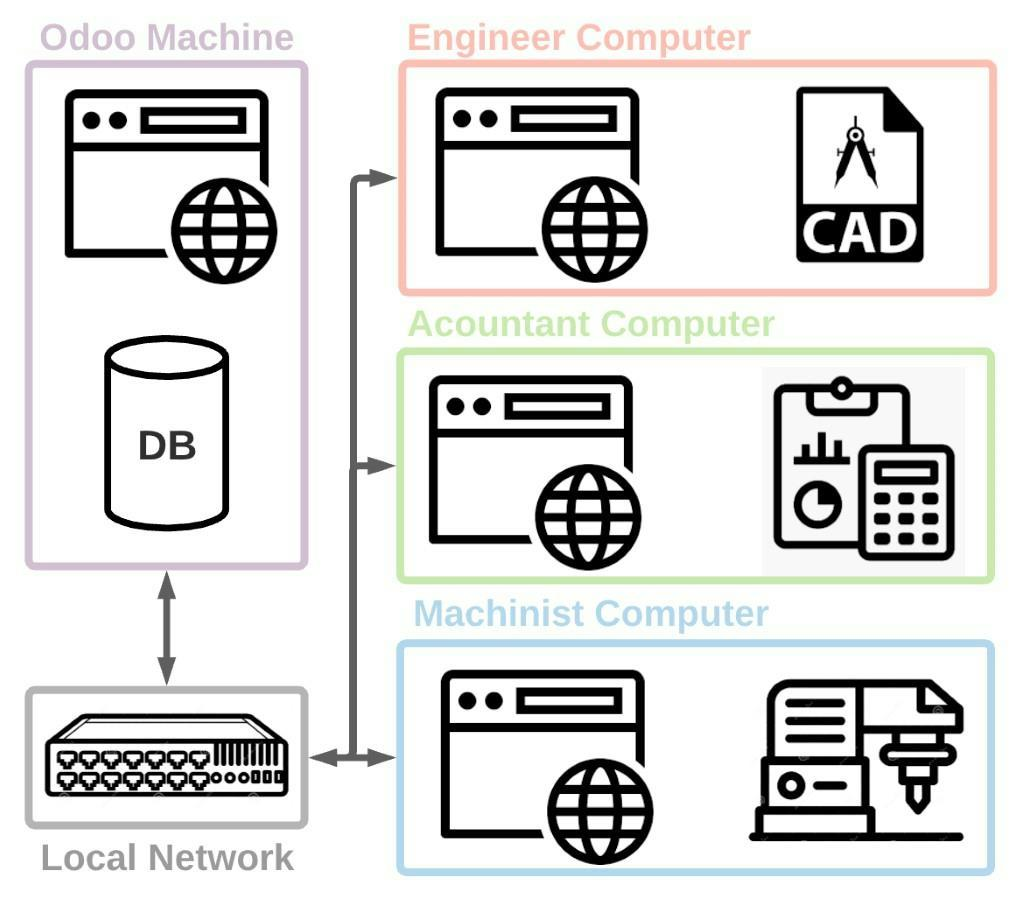
\includegraphics[width=441.8pt,height=397.51pt]{latexImage_9878216f2fc1f6c48a86a10ca880b21c.png}}
\end{picture}
\newpage
\begin{tikzpicture}[overlay]\path(0pt,0pt);\end{tikzpicture}
\begin{picture}(-5,0)(2.5,0)
\put(500.14,-727.616){\fontsize{12}{1}\usefont{T1}{ptm}{m}{n}\selectfont\color{color_29791}25}
\put(512.14,-727.616){\fontsize{12}{1}\usefont{T1}{ptm}{m}{n}\selectfont\color{color_29791} }
\put(515.14,-727.616){\fontsize{12}{1}\usefont{T1}{ptm}{m}{n}\selectfont\color{color_29791} }
\put(70.104,-742.496){\fontsize{10.56}{1}\usefont{T1}{ptm}{m}{n}\selectfont\color{color_29791} }
\put(72.744,-742.496){\fontsize{12}{1}\usefont{T1}{ptm}{m}{n}\selectfont\color{color_29791} }
\put(84.264,-72.09998){\fontsize{12}{1}\usefont{T1}{ptm}{m}{n}\selectfont\color{color_29791}  }
\put(90.26,-72.09998){\fontsize{12}{1}\usefont{T1}{ptm}{m}{n}\selectfont\color{color_29791} }
\put(82.944,-88.06){\fontsize{12}{1}\usefont{T1}{ptm}{m}{n}\selectfont\color{color_29791}另一種選擇是使用}
\put(178.94,-88.06){\fontsize{12}{1}\usefont{T1}{ptm}{m}{n}\selectfont\color{color_29791} }
\put(240.29,-88.06){\fontsize{12}{1}\usefont{T1}{ptm}{m}{n}\selectfont\color{color_29791}Odoo}
\put(267.038,-88.06){\fontsize{12}{1}\usefont{T1}{ptm}{m}{n}\selectfont\color{color_29791} }
\put(328.346,-88.06){\fontsize{12}{1}\usefont{T1}{ptm}{m}{n}\selectfont\color{color_29791}S}
\put(335.054,-88.06){\fontsize{12}{1}\usefont{T1}{ptm}{m}{n}\selectfont\color{color_29791}A}
\put(343.094,-88.06){\fontsize{12}{1}\usefont{T1}{ptm}{m}{n}\selectfont\color{color_29791} }
\put(404.47,-88.06){\fontsize{12}{1}\usefont{T1}{ptm}{m}{n}\selectfont\color{color_29791}提供的託管服務}
\put(488.5,-88.06){\fontsize{12}{1}\usefont{T1}{ptm}{m}{n}\selectfont\color{color_29791}(}
\put(500.5,-88.06){\fontsize{12}{1}\usefont{T1}{ptm}{m}{n}\selectfont\color{color_29791}圖}
\put(512.5,-88.06){\fontsize{12}{1}\usefont{T1}{ptm}{m}{n}\selectfont\color{color_29791} }
\put(69.384,-105.58){\fontsize{12}{1}\usefont{T1}{ptm}{m}{n}\selectfont\color{color_29791}17}
\put(81.384,-105.58){\fontsize{12}{1}\usefont{T1}{ptm}{m}{n}\selectfont\color{color_29791})。}
\put(105.38,-105.58){\fontsize{12}{1}\usefont{T1}{ptm}{m}{n}\selectfont\color{color_29791}在這種情況下}
\put(177.38,-105.58){\fontsize{12}{1}\usefont{T1}{ptm}{m}{n}\selectfont\color{color_29791},}
\put(189.41,-105.58){\fontsize{12}{1}\usefont{T1}{ptm}{m}{n}\selectfont\color{color_29791}系統將由他們託管}
\put(285.41,-105.58){\fontsize{12}{1}\usefont{T1}{ptm}{m}{n}\selectfont\color{color_29791},}
\put(297.41,-105.58){\fontsize{12}{1}\usefont{T1}{ptm}{m}{n}\selectfont\color{color_29791}數據將存儲在他們的雲中}
\put(429.43,-105.58){\fontsize{12}{1}\usefont{T1}{ptm}{m}{n}\selectfont\color{color_29791}。}
\put(441.43,-105.58){\fontsize{12}{1}\usefont{T1}{ptm}{m}{n}\selectfont\color{color_29791}這非常適合}
\put(69.384,-123.22){\fontsize{12}{1}\usefont{T1}{ptm}{m}{n}\selectfont\color{color_29791}許多小型企業}
\put(141.38,-123.22){\fontsize{12}{1}\usefont{T1}{ptm}{m}{n}\selectfont\color{color_29791},}
\put(153.38,-123.22){\fontsize{12}{1}\usefont{T1}{ptm}{m}{n}\selectfont\color{color_29791}特別是如果他們特別喜歡與網站相關的模組}
\put(381.43,-123.22){\fontsize{12}{1}\usefont{T1}{ptm}{m}{n}\selectfont\color{color_29791}(}
\put(393.43,-123.22){\fontsize{12}{1}\usefont{T1}{ptm}{m}{n}\selectfont\color{color_29791}用於構建和管理網站}
\put(69.384,-140.98){\fontsize{12}{1}\usefont{T1}{ptm}{m}{n}\selectfont\color{color_29791}和電子商店}
\put(129.38,-140.98){\fontsize{12}{1}\usefont{T1}{ptm}{m}{n}\selectfont\color{color_29791})。}
\put(153.38,-140.98){\fontsize{12}{1}\usefont{T1}{ptm}{m}{n}\selectfont\color{color_29791}但是}
\put(177.38,-140.98){\fontsize{12}{1}\usefont{T1}{ptm}{m}{n}\selectfont\color{color_29791},}
\put(189.41,-140.98){\fontsize{12}{1}\usefont{T1}{ptm}{m}{n}\selectfont\color{color_29791}它依賴於網路}
\put(261.41,-140.98){\fontsize{12}{1}\usefont{T1}{ptm}{m}{n}\selectfont\color{color_29791},}
\put(273.41,-140.98){\fontsize{12}{1}\usefont{T1}{ptm}{m}{n}\selectfont\color{color_29791}在某些情況下可能會帶來問題}
\put(429.43,-140.98){\fontsize{12}{1}\usefont{T1}{ptm}{m}{n}\selectfont\color{color_29791}。}
\put(441.43,-140.98){\fontsize{12}{1}\usefont{T1}{ptm}{m}{n}\selectfont\color{color_29791}   }
\put(450.46,-140.98){\fontsize{12}{1}\usefont{T1}{ptm}{m}{n}\selectfont\color{color_29791} }
\put(84.264,-158.5){\fontsize{12}{1}\usefont{T1}{ptm}{m}{n}\selectfont\color{color_29791} }
\put(87.26,-158.5){\fontsize{12}{1}\usefont{T1}{ptm}{m}{n}\selectfont\color{color_29791} }
\put(515.74,-447.03){\fontsize{12}{1}\usefont{T1}{ptm}{m}{n}\selectfont\color{color_29791} }
\put(518.74,-447.03){\fontsize{12}{1}\usefont{T1}{ptm}{m}{n}\selectfont\color{color_29791} }
\put(229.37,-459.51){\fontsize{12}{1}\usefont{T1}{ptm}{m}{n}\selectfont\color{color_29791}圖}
\put(241.49,-459.51){\fontsize{12}{1}\usefont{T1}{ptm}{b}{n}\selectfont\color{color_29791}17 }
\put(256.49,-459.51){\fontsize{12}{1}\usefont{T1}{ptm}{b}{n}\selectfont\color{color_29791}Od}
\put(272.558,-459.51){\fontsize{12}{1}\usefont{T1}{ptm}{b}{n}\selectfont\color{color_29791}oo}
\put(284.45,-459.51){\fontsize{12}{1}\usefont{T1}{ptm}{m}{n}\selectfont\color{color_29791}配置}
\put(308.45,-459.51){\fontsize{12}{1}\usefont{T1}{ptm}{b}{n}\selectfont\color{color_29791}B}
\put(316.51,-459.51){\fontsize{12}{1}\usefont{T1}{ptm}{m}{n}\selectfont\color{color_29791}功能圖}
\put(352.63,-459.51){\fontsize{12}{1}\usefont{T1}{ptm}{b}{n}\selectfont\color{color_29791} }
\put(355.51,-459.51){\fontsize{12}{1}\usefont{T1}{ptm}{m}{n}\selectfont\color{color_29791} }
\put(84.264,-476.91){\fontsize{12}{1}\usefont{T1}{ptm}{m}{n}\selectfont\color{color_29791}  }
\put(90.26,-476.91){\fontsize{12}{1}\usefont{T1}{ptm}{m}{n}\selectfont\color{color_29791} }
\put(82.944,-492.99){\fontsize{12}{1}\usefont{T1}{ptm}{m}{n}\selectfont\color{color_29791}使用者基本上通過圖形使用者介面}
\put(262.97,-492.99){\fontsize{12}{1}\usefont{T1}{ptm}{m}{n}\selectfont\color{color_29791} }
\put(467.14,-492.99){\fontsize{12}{1}\usefont{T1}{ptm}{m}{n}\selectfont\color{color_29791}(}
\put(479.14,-492.99){\fontsize{12}{1}\usefont{T1}{ptm}{m}{n}\selectfont\color{color_29791}GU}
\put(496.528,-492.99){\fontsize{12}{1}\usefont{T1}{ptm}{m}{n}\selectfont\color{color_29791}I}
\put(500.38,-492.99){\fontsize{12}{1}\usefont{T1}{ptm}{m}{n}\selectfont\color{color_29791})}
\put(512.5,-492.99){\fontsize{12}{1}\usefont{T1}{ptm}{m}{n}\selectfont\color{color_29791} }
\put(69.384,-510.51){\fontsize{12}{1}\usefont{T1}{ptm}{m}{n}\selectfont\color{color_29791}與系統交互}
\put(129.38,-510.51){\fontsize{12}{1}\usefont{T1}{ptm}{m}{n}\selectfont\color{color_29791},}
\put(141.38,-510.51){\fontsize{12}{1}\usefont{T1}{ptm}{m}{n}\selectfont\color{color_29791}並使用它來訪問每個用戶根據需要提供的不同模組}
\put(405.43,-510.51){\fontsize{12}{1}\usefont{T1}{ptm}{m}{n}\selectfont\color{color_29791}。}
\put(417.43,-510.51){\fontsize{12}{1}\usefont{T1}{ptm}{m}{n}\selectfont\color{color_29791} }
\put(69.384,-528.15){\fontsize{12}{1}\usefont{T1}{ptm}{m}{n}\selectfont\color{color_29791}這意味著可以對不同的使用者施加限制}
\put(273.41,-528.15){\fontsize{12}{1}\usefont{T1}{ptm}{m}{n}\selectfont\color{color_29791},}
\put(285.41,-528.15){\fontsize{12}{1}\usefont{T1}{ptm}{m}{n}\selectfont\color{color_29791}以保持對商務活動不同方面的控制}
\put(465.46,-528.15){\fontsize{12}{1}\usefont{T1}{ptm}{m}{n}\selectfont\color{color_29791},}
\put(477.46,-528.15){\fontsize{12}{1}\usefont{T1}{ptm}{m}{n}\selectfont\color{color_29791}例如}
\put(69.384,-545.79){\fontsize{12}{1}\usefont{T1}{ptm}{m}{n}\selectfont\color{color_29791},}
\put(81.384,-545.79){\fontsize{12}{1}\usefont{T1}{ptm}{m}{n}\selectfont\color{color_29791}會計師可以訪問會計模組}
\put(213.41,-545.79){\fontsize{12}{1}\usefont{T1}{ptm}{m}{n}\selectfont\color{color_29791}、}
\put(225.41,-545.79){\fontsize{12}{1}\usefont{T1}{ptm}{m}{n}\selectfont\color{color_29791}銷售模組和庫存模組}
\put(333.43,-545.79){\fontsize{12}{1}\usefont{T1}{ptm}{m}{n}\selectfont\color{color_29791},}
\put(345.43,-545.79){\fontsize{12}{1}\usefont{T1}{ptm}{m}{n}\selectfont\color{color_29791}但他們將受到製造模組的限制}
\put(69.384,-563.55){\fontsize{12}{1}\usefont{T1}{ptm}{m}{n}\selectfont\color{color_29791}。}
\put(81.384,-563.55){\fontsize{12}{1}\usefont{T1}{ptm}{m}{n}\selectfont\color{color_29791}這種限制保證了對流程的控制只對適當的員工}
\put(321.43,-563.55){\fontsize{12}{1}\usefont{T1}{ptm}{m}{n}\selectfont\color{color_29791}。}
\put(333.43,-563.55){\fontsize{12}{1}\usefont{T1}{ptm}{m}{n}\selectfont\color{color_29791}   }
\put(342.43,-563.55){\fontsize{12}{1}\usefont{T1}{ptm}{m}{n}\selectfont\color{color_29791} }
\put(84.264,-581.07){\fontsize{12}{1}\usefont{T1}{ptm}{m}{n}\selectfont\color{color_29791}  }
\put(90.26,-581.07){\fontsize{12}{1}\usefont{T1}{ptm}{m}{n}\selectfont\color{color_29791} }
\put(82.944,-596.22){\fontsize{12}{1}\usefont{T1}{ptm}{m}{n}\selectfont\color{color_29791}在上述}
\put(118.94,-596.22){\fontsize{12}{1}\usefont{T1}{ptm}{m}{n}\selectfont\color{color_29791} }
\put(197.09,-596.22){\fontsize{12}{1}\usefont{T1}{ptm}{m}{n}\selectfont\color{color_29791}GU}
\put(214.478,-596.22){\fontsize{12}{1}\usefont{T1}{ptm}{m}{n}\selectfont\color{color_29791}I}
\put(218.198,-596.22){\fontsize{12}{1}\usefont{T1}{ptm}{m}{n}\selectfont\color{color_29791} }
\put(296.33,-596.22){\fontsize{12}{1}\usefont{T1}{ptm}{m}{n}\selectfont\color{color_29791}中}
\put(308.33,-596.22){\fontsize{12}{1}\usefont{T1}{ptm}{m}{n}\selectfont\color{color_29791},}
\put(320.47,-596.22){\fontsize{12}{1}\usefont{T1}{ptm}{m}{n}\selectfont\color{color_29791}不同的模組顯示為應用程式圖示}
\put(488.5,-596.22){\fontsize{12}{1}\usefont{T1}{ptm}{m}{n}\selectfont\color{color_29791}(}
\put(500.5,-596.22){\fontsize{12}{1}\usefont{T1}{ptm}{m}{n}\selectfont\color{color_29791}圖}
\put(512.5,-596.22){\fontsize{12}{1}\usefont{T1}{ptm}{m}{n}\selectfont\color{color_29791} }
\put(69.384,-613.86){\fontsize{12}{1}\usefont{T1}{ptm}{m}{n}\selectfont\color{color_29791}18}
\put(81.384,-613.86){\fontsize{12}{1}\usefont{T1}{ptm}{m}{n}\selectfont\color{color_29791}),}
\put(105.38,-613.86){\fontsize{12}{1}\usefont{T1}{ptm}{m}{n}\selectfont\color{color_29791}從一開始}
\put(153.38,-613.86){\fontsize{12}{1}\usefont{T1}{ptm}{m}{n}\selectfont\color{color_29791},}
\put(165.38,-613.86){\fontsize{12}{1}\usefont{T1}{ptm}{m}{n}\selectfont\color{color_29791}該公司就提供了合理選擇的集成良好的應用程式}
\put(417.43,-613.86){\fontsize{12}{1}\usefont{T1}{ptm}{m}{n}\selectfont\color{color_29791},}
\put(429.43,-613.86){\fontsize{12}{1}\usefont{T1}{ptm}{m}{n}\selectfont\color{color_29791}更不用說充滿}
\put(69.384,-631.5){\fontsize{12}{1}\usefont{T1}{ptm}{m}{n}\selectfont\color{color_29791}社區製作模組的龐大應用程式商店了}
\put(261.41,-631.5){\fontsize{12}{1}\usefont{T1}{ptm}{m}{n}\selectfont\color{color_29791}。}
\put(273.41,-631.5){\fontsize{12}{1}\usefont{T1}{ptm}{m}{n}\selectfont\color{color_29791}  }
\put(279.41,-631.5){\fontsize{12}{1}\usefont{T1}{ptm}{m}{n}\selectfont\color{color_29791} }
\put(84.264,-649.02){\fontsize{12}{1}\usefont{T1}{ptm}{m}{n}\selectfont\color{color_29791} }
\put(87.26,-649.02){\fontsize{12}{1}\usefont{T1}{ptm}{m}{n}\selectfont\color{color_29791} }
\put(73.75,-446.9801){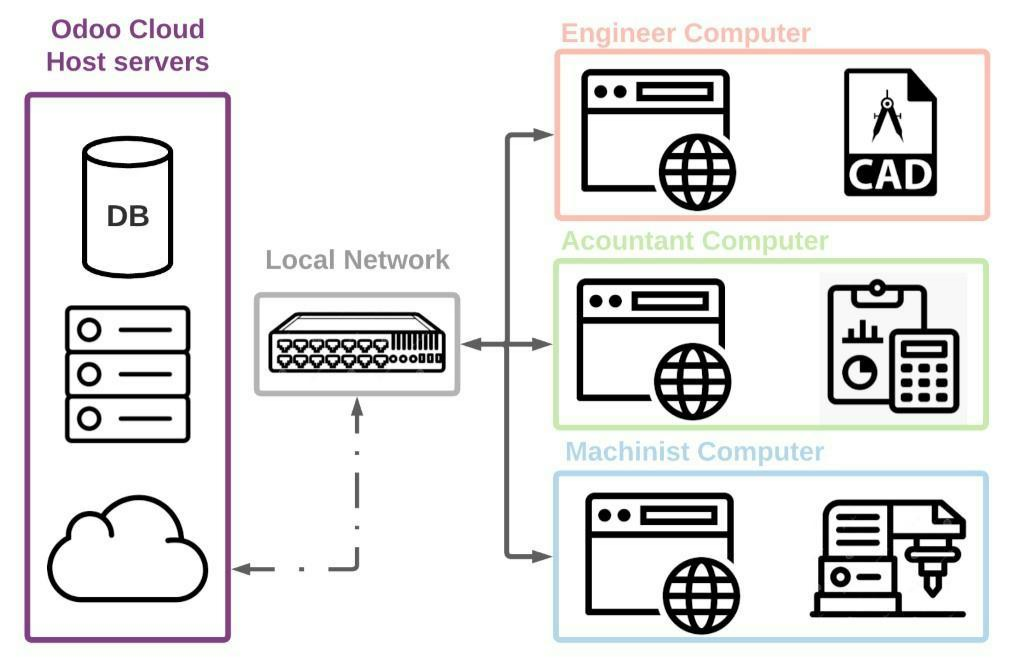
\includegraphics[width=441.9pt,height=284.8pt]{latexImage_c03f17f9f62a42dc50df2d2b5e5dde5b.png}}
\end{picture}
\newpage
\begin{tikzpicture}[overlay]\path(0pt,0pt);\end{tikzpicture}
\begin{picture}(-5,0)(2.5,0)
\put(500.14,-727.616){\fontsize{12}{1}\usefont{T1}{ptm}{m}{n}\selectfont\color{color_29791}26}
\put(512.14,-727.616){\fontsize{12}{1}\usefont{T1}{ptm}{m}{n}\selectfont\color{color_29791} }
\put(515.14,-727.616){\fontsize{12}{1}\usefont{T1}{ptm}{m}{n}\selectfont\color{color_29791} }
\put(70.104,-742.496){\fontsize{10.56}{1}\usefont{T1}{ptm}{m}{n}\selectfont\color{color_29791} }
\put(72.744,-742.496){\fontsize{12}{1}\usefont{T1}{ptm}{m}{n}\selectfont\color{color_29791} }
\put(515.74,-215.98){\fontsize{12}{1}\usefont{T1}{ptm}{m}{n}\selectfont\color{color_29791} }
\put(518.74,-215.98){\fontsize{12}{1}\usefont{T1}{ptm}{m}{n}\selectfont\color{color_29791} }
\put(189.53,-238.66){\fontsize{12}{1}\usefont{T1}{ptm}{m}{n}\selectfont\color{color_29791}圖}
\put(201.65,-238.66){\fontsize{12}{1}\usefont{T1}{ptm}{b}{n}\selectfont\color{color_29791} }
\put(204.65,-238.66){\fontsize{12}{1}\usefont{T1}{ptm}{b}{n}\selectfont\color{color_29791}18 }
\put(219.53,-238.66){\fontsize{12}{1}\usefont{T1}{ptm}{m}{n}\selectfont\color{color_29791}配置}
\put(243.65,-238.66){\fontsize{12}{1}\usefont{T1}{ptm}{b}{n}\selectfont\color{color_29791} }
\put(246.65,-238.66){\fontsize{12}{1}\usefont{T1}{ptm}{b}{n}\selectfont\color{color_29791}B }
\put(257.57,-238.66){\fontsize{12}{1}\usefont{T1}{ptm}{m}{n}\selectfont\color{color_29791}中}
\put(269.69,-238.66){\fontsize{12}{1}\usefont{T1}{ptm}{b}{n}\selectfont\color{color_29791} }
\put(272.69,-238.66){\fontsize{12}{1}\usefont{T1}{ptm}{b}{n}\selectfont\color{color_29791}Od}
\put(288.77,-238.66){\fontsize{12}{1}\usefont{T1}{ptm}{b}{n}\selectfont\color{color_29791}oo }
\put(303.65,-238.66){\fontsize{12}{1}\usefont{T1}{ptm}{m}{n}\selectfont\color{color_29791}的}
\put(315.79,-238.66){\fontsize{12}{1}\usefont{T1}{ptm}{b}{n}\selectfont\color{color_29791} }
\put(318.79,-238.66){\fontsize{12}{1}\usefont{T1}{ptm}{b}{n}\selectfont\color{color_29791}G}
\put(328.03,-238.66){\fontsize{12}{1}\usefont{T1}{ptm}{b}{n}\selectfont\color{color_29791}UI }
\put(344.35,-238.66){\fontsize{12}{1}\usefont{T1}{ptm}{m}{n}\selectfont\color{color_29791}螢幕截圖}
\put(392.47,-238.66){\fontsize{12}{1}\usefont{T1}{ptm}{b}{n}\selectfont\color{color_29791} }
\put(395.35,-238.66){\fontsize{12}{1}\usefont{T1}{ptm}{m}{n}\selectfont\color{color_29791} }
\put(106.1,-278.05){\fontsize{12.96}{1}\usefont{T1}{ptm}{b}{n}\selectfont\color{color_29791}5.1.2. Od}
\put(155.8923,-278.05){\fontsize{12.96}{1}\usefont{T1}{ptm}{b}{n}\selectfont\color{color_29791}oo}
\put(168.86,-278.05){\fontsize{12.96}{1}\usefont{T1}{ptm}{m}{n}\selectfont\color{color_29791}對}
\put(181.9237,-278.05){\fontsize{12.96}{1}\usefont{T1}{ptm}{m}{n}\selectfont\color{color_29791}製}
\put(194.9874,-278.05){\fontsize{12.96}{1}\usefont{T1}{ptm}{m}{n}\selectfont\color{color_29791}造}
\put(208.051,-278.05){\fontsize{12.96}{1}\usefont{T1}{ptm}{m}{n}\selectfont\color{color_29791}業的}
\put(234.0747,-278.05){\fontsize{12.96}{1}\usefont{T1}{ptm}{m}{n}\selectfont\color{color_29791}看法}
\put(260.21,-278.05){\fontsize{12.96}{1}\usefont{T1}{ptm}{m}{n}\selectfont\color{color_29791}:}
\put(273.29,-278.05){\fontsize{12.96}{1}\usefont{T1}{ptm}{b}{n}\selectfont\color{color_29791}   }
\put(282.89,-278.05){\fontsize{12.96}{1}\usefont{T1}{ptm}{b}{n}\selectfont\color{color_29791} }
\put(82.944,-307.09){\fontsize{12}{1}\usefont{T1}{ptm}{m}{n}\selectfont\color{color_29791}Odoo}
\put(109.58,-307.09){\fontsize{12}{1}\usefont{T1}{ptm}{m}{n}\selectfont\color{color_29791}認為}
\put(133.58,-307.09){\fontsize{12}{1}\usefont{T1}{ptm}{m}{n}\selectfont\color{color_29791},}
\put(145.58,-307.09){\fontsize{12}{1}\usefont{T1}{ptm}{m}{n}\selectfont\color{color_29791}製造任何產品的責任都分佈在不同的公司部門}
\put(385.63,-307.09){\fontsize{12}{1}\usefont{T1}{ptm}{m}{n}\selectfont\color{color_29791},}
\put(397.63,-307.09){\fontsize{12}{1}\usefont{T1}{ptm}{m}{n}\selectfont\color{color_29791}每個部門負責特定的}
\put(69.384,-324.73){\fontsize{12}{1}\usefont{T1}{ptm}{m}{n}\selectfont\color{color_29791}檔類型}
\put(105.38,-324.73){\fontsize{12}{1}\usefont{T1}{ptm}{m}{n}\selectfont\color{color_29791},}
\put(117.38,-324.73){\fontsize{12}{1}\usefont{T1}{ptm}{m}{n}\selectfont\color{color_29791}並使用特定的應用程式進行處理}
\put(285.41,-324.73){\fontsize{12}{1}\usefont{T1}{ptm}{m}{n}\selectfont\color{color_29791}(}
\put(297.41,-324.73){\fontsize{12}{1}\usefont{T1}{ptm}{m}{n}\selectfont\color{color_29791}表}
\put(309.41,-324.73){\fontsize{12}{1}\usefont{T1}{ptm}{m}{n}\selectfont\color{color_29791}2}
\put(315.43,-324.73){\fontsize{12}{1}\usefont{T1}{ptm}{m}{n}\selectfont\color{color_29791})。}
\put(339.43,-324.73){\fontsize{12}{1}\usefont{T1}{ptm}{m}{n}\selectfont\color{color_29791}從}
\put(351.43,-324.73){\fontsize{12}{1}\usefont{T1}{ptm}{m}{n}\selectfont\color{color_29791}P}
\put(358.258,-324.73){\fontsize{12}{1}\usefont{T1}{ptm}{m}{n}\selectfont\color{color_29791}L}
\put(365.338,-324.73){\fontsize{12}{1}\usefont{T1}{ptm}{m}{n}\selectfont\color{color_29791}M}
\put(376.03,-324.73){\fontsize{12}{1}\usefont{T1}{ptm}{m}{n}\selectfont\color{color_29791}的角度來}
\put(424.138,-324.73){\fontsize{12}{1}\usefont{T1}{ptm}{m}{n}\selectfont\color{color_29791}看}
\put(436.15,-324.73){\fontsize{12}{1}\usefont{T1}{ptm}{m}{n}\selectfont\color{color_29791},}
\put(448.18,-324.73){\fontsize{12}{1}\usefont{T1}{ptm}{m}{n}\selectfont\color{color_29791}這是非常積}
\put(69.384,-342.37){\fontsize{12}{1}\usefont{T1}{ptm}{m}{n}\selectfont\color{color_29791}極的}
\put(93.38,-342.37){\fontsize{12}{1}\usefont{T1}{ptm}{m}{n}\selectfont\color{color_29791},}
\put(105.38,-342.37){\fontsize{12}{1}\usefont{T1}{ptm}{m}{n}\selectfont\color{color_29791}因為正如}
\put(153.38,-342.37){\fontsize{12}{1}\usefont{T1}{ptm}{m}{n}\selectfont\color{color_29791}(}
\put(165.38,-342.37){\fontsize{12}{1}\usefont{T1}{ptm}{m}{n}\selectfont\color{color_29791}S}
\put(172.088,-342.37){\fontsize{12}{1}\usefont{T1}{ptm}{m}{n}\selectfont\color{color_29791}a}
\put(177.368,-342.37){\fontsize{12}{1}\usefont{T1}{ptm}{m}{n}\selectfont\color{color_29791}a}
\put(182.648,-342.37){\fontsize{12}{1}\usefont{T1}{ptm}{m}{n}\selectfont\color{color_29791}ksvuori}
\put(218.69,-342.37){\fontsize{12}{1}\usefont{T1}{ptm}{m}{n}\selectfont\color{color_29791}和}
\put(230.81,-342.37){\fontsize{12}{1}\usefont{T1}{ptm}{m}{n}\selectfont\color{color_29791}I}
\put(234.53,-342.37){\fontsize{12}{1}\usefont{T1}{ptm}{m}{n}\selectfont\color{color_29791}mm}
\put(253.238,-342.37){\fontsize{12}{1}\usefont{T1}{ptm}{m}{n}\selectfont\color{color_29791}one}
\put(270.518,-342.37){\fontsize{12}{1}\usefont{T1}{ptm}{m}{n}\selectfont\color{color_29791}n}
\put(276.53,-342.37){\fontsize{12}{1}\usefont{T1}{ptm}{m}{n}\selectfont\color{color_29791},}
\put(288.53,-342.37){\fontsize{12}{1}\usefont{T1}{ptm}{m}{n}\selectfont\color{color_29791}200}
\put(306.638,-342.37){\fontsize{12}{1}\usefont{T1}{ptm}{m}{n}\selectfont\color{color_29791}8}
\put(312.67,-342.37){\fontsize{12}{1}\usefont{T1}{ptm}{m}{n}\selectfont\color{color_29791})}
\put(324.67,-342.37){\fontsize{12}{1}\usefont{T1}{ptm}{m}{n}\selectfont\color{color_29791}關於用戶許可權管理所提到的}
\put(480.7,-342.37){\fontsize{12}{1}\usefont{T1}{ptm}{m}{n}\selectfont\color{color_29791},}
\put(492.7,-342.37){\fontsize{12}{1}\usefont{T1}{ptm}{m}{n}\selectfont\color{color_29791}PL}
\put(69.384,-360.01){\fontsize{12}{1}\usefont{T1}{ptm}{m}{n}\selectfont\color{color_29791}M}
\put(80.064,-360.01){\fontsize{12}{1}\usefont{T1}{ptm}{m}{n}\selectfont\color{color_29791}系統用於定義資訊訪問和維護許可權}
\put(272.09,-360.01){\fontsize{12}{1}\usefont{T1}{ptm}{m}{n}\selectfont\color{color_29791}。}
\put(284.09,-360.01){\fontsize{12}{1}\usefont{T1}{ptm}{m}{n}\selectfont\color{color_29791}P}
\put(290.918,-360.01){\fontsize{12}{1}\usefont{T1}{ptm}{m}{n}\selectfont\color{color_29791}L}
\put(297.998,-360.01){\fontsize{12}{1}\usefont{T1}{ptm}{m}{n}\selectfont\color{color_29791}M}
\put(308.786,-360.01){\fontsize{12}{1}\usefont{T1}{ptm}{m}{n}\selectfont\color{color_29791} }
\put(69.384,-377.65){\fontsize{12}{1}\usefont{T1}{ptm}{m}{n}\selectfont\color{color_29791}系統定義了可以創建新資訊或進行}
\put(249.41,-377.65){\fontsize{12}{1}\usefont{T1}{ptm}{m}{n}\selectfont\color{color_29791}、}
\put(261.41,-377.65){\fontsize{12}{1}\usefont{T1}{ptm}{m}{n}\selectfont\color{color_29791}檢查和接受更改的人員}
\put(381.43,-377.65){\fontsize{12}{1}\usefont{T1}{ptm}{m}{n}\selectfont\color{color_29791},}
\put(393.43,-377.65){\fontsize{12}{1}\usefont{T1}{ptm}{m}{n}\selectfont\color{color_29791}以及僅允許查看系統}
\put(69.384,-395.29){\fontsize{12}{1}\usefont{T1}{ptm}{m}{n}\selectfont\color{color_29791}中的資訊或文檔的人員}
\put(189.41,-395.29){\fontsize{12}{1}\usefont{T1}{ptm}{m}{n}\selectfont\color{color_29791}。}
\put(201.41,-395.29){\fontsize{12}{1}\usefont{T1}{ptm}{m}{n}\selectfont\color{color_29791}在將}
\put(225.41,-395.29){\fontsize{12}{1}\usefont{T1}{ptm}{m}{n}\selectfont\color{color_29791} }
\put(487.9,-395.29){\fontsize{12}{1}\usefont{T1}{ptm}{m}{n}\selectfont\color{color_29791}P}
\put(494.728,-395.29){\fontsize{12}{1}\usefont{T1}{ptm}{m}{n}\selectfont\color{color_29791}L}
\put(501.808,-395.29){\fontsize{12}{1}\usefont{T1}{ptm}{m}{n}\selectfont\color{color_29791}M }
\put(69.384,-413.05){\fontsize{12}{1}\usefont{T1}{ptm}{m}{n}\selectfont\color{color_29791}與其他系統整合時}
\put(165.38,-413.05){\fontsize{12}{1}\usefont{T1}{ptm}{m}{n}\selectfont\color{color_29791},}
\put(177.38,-413.05){\fontsize{12}{1}\usefont{T1}{ptm}{m}{n}\selectfont\color{color_29791}用戶許可權管理通常是}
\put(297.41,-413.05){\fontsize{12}{1}\usefont{T1}{ptm}{m}{n}\selectfont\color{color_29791}一個挑戰}
\put(345.43,-413.05){\fontsize{12}{1}\usefont{T1}{ptm}{m}{n}\selectfont\color{color_29791}。}
\put(357.43,-413.05){\fontsize{12}{1}\usefont{T1}{ptm}{m}{n}\selectfont\color{color_29791}   }
\put(366.43,-413.05){\fontsize{12}{1}\usefont{T1}{ptm}{m}{n}\selectfont\color{color_29791} }
\put(84.264,-430.47){\fontsize{12}{1}\usefont{T1}{ptm}{m}{n}\selectfont\color{color_29791} }
\put(87.26,-430.47){\fontsize{12}{1}\usefont{T1}{ptm}{m}{n}\selectfont\color{color_29791} }
\put(202.13,-446.43){\fontsize{12}{1}\usefont{T1}{ptm}{m}{n}\selectfont\color{color_29791}表}
\put(214.25,-446.43){\fontsize{12}{1}\usefont{T1}{ptm}{b}{n}\selectfont\color{color_29791}2}
\put(220.13,-446.43){\fontsize{12}{1}\usefont{T1}{ptm}{m}{n}\selectfont\color{color_29791}部門與}
\put(256.238,-446.43){\fontsize{12}{1}\usefont{T1}{ptm}{m}{n}\selectfont\color{color_29791}文檔}
\put(280.25,-446.43){\fontsize{12}{1}\usefont{T1}{ptm}{b}{n}\selectfont\color{color_29791}/}
\put(283.61,-446.43){\fontsize{12}{1}\usefont{T1}{ptm}{m}{n}\selectfont\color{color_29791}應用程式的相關}
\put(367.718,-446.43){\fontsize{12}{1}\usefont{T1}{ptm}{m}{n}\selectfont\color{color_29791}性}
\put(379.87,-446.43){\fontsize{12}{1}\usefont{T1}{ptm}{b}{n}\selectfont\color{color_29791} }
\put(382.75,-446.43){\fontsize{12}{1}\usefont{T1}{ptm}{m}{n}\selectfont\color{color_29791} }
\end{picture}
\begin{tikzpicture}[overlay]
\path(0pt,0pt);
\filldraw[color_255811][even odd rule]
(70.104pt, -477.51pt) -- (290.564pt, -477.51pt)
 -- (290.564pt, -477.51pt)
 -- (290.564pt, -452.55pt)
 -- (290.564pt, -452.55pt)
 -- (70.104pt, -452.55pt) -- cycle
;
\begin{scope}
\clip
(70.104pt, -477.51pt) -- (290.564pt, -477.51pt)
 -- (290.564pt, -477.51pt)
 -- (290.564pt, -454.95pt)
 -- (290.564pt, -454.95pt)
 -- (70.104pt, -454.95pt) -- cycle
;
\filldraw[color_255811][even odd rule]
(75.504pt, -477.39pt) -- (285.284pt, -477.39pt)
 -- (285.284pt, -477.39pt)
 -- (285.284pt, -454.95pt)
 -- (285.284pt, -454.95pt)
 -- (75.504pt, -454.95pt) -- cycle
;
\begin{scope}
\clip
(70.104pt, -477.51pt) -- (290.564pt, -477.51pt)
 -- (290.564pt, -477.51pt)
 -- (290.564pt, -454.95pt)
 -- (290.564pt, -454.95pt)
 -- (70.104pt, -454.95pt) -- cycle
;
\end{scope}
\end{scope}
\end{tikzpicture}
\begin{picture}(-5,0)(2.5,0)
\put(164.18,-470.19){\fontsize{15.96}{1}\usefont{T1}{ptm}{m}{n}\selectfont\color{color_29791}部門}
\put(196.37,-470.19){\fontsize{15.96}{1}\usefont{T1}{ptm}{b}{n}\selectfont\color{color_29791} }
\put(199.85,-470.19){\fontsize{12}{1}\usefont{T1}{ptm}{m}{n}\selectfont\color{color_29791} }
\end{picture}
\begin{tikzpicture}[overlay]
\path(0pt,0pt);
\filldraw[color_215151][even odd rule]
(291.05pt, -477.51pt) -- (511.66pt, -477.51pt)
 -- (511.66pt, -477.51pt)
 -- (511.66pt, -452.55pt)
 -- (511.66pt, -452.55pt)
 -- (291.05pt, -452.55pt) -- cycle
;
\begin{scope}
\clip
(291.05pt, -477.51pt) -- (511.66pt, -477.51pt)
 -- (511.66pt, -477.51pt)
 -- (511.66pt, -454.95pt)
 -- (511.66pt, -454.95pt)
 -- (291.05pt, -454.95pt) -- cycle
;
\filldraw[color_215151][even odd rule]
(296.21pt, -477.51pt) -- (506.14pt, -477.51pt)
 -- (506.14pt, -477.51pt)
 -- (506.14pt, -454.95pt)
 -- (506.14pt, -454.95pt)
 -- (296.21pt, -454.95pt) -- cycle
;
\begin{scope}
\clip
(291.05pt, -477.51pt) -- (511.66pt, -477.51pt)
 -- (511.66pt, -477.51pt)
 -- (511.66pt, -454.95pt)
 -- (511.66pt, -454.95pt)
 -- (291.05pt, -454.95pt) -- cycle
;
\end{scope}
\end{scope}
\end{tikzpicture}
\begin{picture}(-5,0)(2.5,0)
\put(349.51,-470.19){\fontsize{15.96}{1}\usefont{T1}{ptm}{m}{n}\selectfont\color{color_29791}文件}
\put(381.67,-470.19){\fontsize{15.96}{1}\usefont{T1}{ptm}{b}{n}\selectfont\color{color_29791}/}
\put(388.51,-470.19){\fontsize{15.96}{1}\usefont{T1}{ptm}{m}{n}\selectfont\color{color_29791}應用}
\put(420.5417,-470.19){\fontsize{15.96}{1}\usefont{T1}{ptm}{m}{n}\selectfont\color{color_29791}程式}
\put(452.62,-470.19){\fontsize{15.96}{1}\usefont{T1}{ptm}{b}{n}\selectfont\color{color_29791} }
\put(456.1,-470.19){\fontsize{12}{1}\usefont{T1}{ptm}{m}{n}\selectfont\color{color_29791} }
\end{picture}
\begin{tikzpicture}[overlay]
\path(0pt,0pt);
\filldraw[color_255811][even odd rule]
(70.104pt, -454.95pt) -- (290.564pt, -454.95pt)
 -- (290.564pt, -454.95pt)
 -- (290.564pt, -452.55pt)
 -- (290.564pt, -452.55pt)
 -- (70.104pt, -452.55pt) -- cycle
;
\filldraw[color_29791][even odd rule]
(290.57pt, -454.95pt) -- (291.05pt, -454.95pt)
 -- (291.05pt, -454.95pt)
 -- (291.05pt, -452.55pt)
 -- (291.05pt, -452.55pt)
 -- (290.57pt, -452.55pt) -- cycle
;
\filldraw[color_215151][even odd rule]
(290.57pt, -454.95pt) -- (511.66pt, -454.95pt)
 -- (511.66pt, -454.95pt)
 -- (511.66pt, -452.55pt)
 -- (511.66pt, -452.55pt)
 -- (290.57pt, -452.55pt) -- cycle
;
\filldraw[color_29791][even odd rule]
(290.57pt, -477.51pt) -- (291.05pt, -477.51pt)
 -- (291.05pt, -477.51pt)
 -- (291.05pt, -454.95pt)
 -- (291.05pt, -454.95pt)
 -- (290.57pt, -454.95pt) -- cycle
;
\begin{scope}
\clip
(70.104pt, -496.83pt) -- (290.564pt, -496.83pt)
 -- (290.564pt, -496.83pt)
 -- (290.564pt, -479.91pt)
 -- (290.564pt, -479.91pt)
 -- (70.104pt, -479.91pt) -- cycle
;
\begin{scope}
\clip
(70.104pt, -496.83pt) -- (290.564pt, -496.83pt)
 -- (290.564pt, -496.83pt)
 -- (290.564pt, -479.91pt)
 -- (290.564pt, -479.91pt)
 -- (70.104pt, -479.91pt) -- cycle
;
\end{scope}
\end{scope}
\end{tikzpicture}
\begin{picture}(-5,0)(2.5,0)
\put(75.504,-491.31){\fontsize{12}{1}\usefont{T1}{ptm}{m}{n}\selectfont\color{color_29791}工程}
\put(99.5,-491.31){\fontsize{12}{1}\usefont{T1}{ptm}{m}{n}\selectfont\color{color_29791}  }
\put(104.9,-491.31){\fontsize{12}{1}\usefont{T1}{ptm}{m}{n}\selectfont\color{color_29791} }
\put(296.21,-491.31){\fontsize{12}{1}\usefont{T1}{ptm}{m}{n}\selectfont\color{color_29791}C}
\put(302.57,-491.31){\fontsize{12}{1}\usefont{T1}{ptm}{m}{n}\selectfont\color{color_29791}AD}
\put(316.958,-491.31){\fontsize{12}{1}\usefont{T1}{ptm}{m}{n}\selectfont\color{color_29791} }
\put(319.75,-491.31){\fontsize{12}{1}\usefont{T1}{ptm}{m}{n}\selectfont\color{color_29791}和}
\put(331.75,-491.31){\fontsize{12}{1}\usefont{T1}{ptm}{m}{n}\selectfont\color{color_29791} }
\put(334.51,-491.31){\fontsize{12}{1}\usefont{T1}{ptm}{m}{n}\selectfont\color{color_29791}B}
\put(340.99,-491.31){\fontsize{12}{1}\usefont{T1}{ptm}{m}{n}\selectfont\color{color_29791}OM}
\put(359.218,-491.31){\fontsize{12}{1}\usefont{T1}{ptm}{m}{n}\selectfont\color{color_29791} }
\put(361.858,-491.31){\fontsize{12}{1}\usefont{T1}{ptm}{m}{n}\selectfont\color{color_29791} }
\put(364.51,-491.31){\fontsize{12}{1}\usefont{T1}{ptm}{m}{n}\selectfont\color{color_29791} }
\end{picture}
\begin{tikzpicture}[overlay]
\path(0pt,0pt);
\filldraw[color_29791][even odd rule]
(290.57pt, -479.91pt) -- (291.05pt, -479.91pt)
 -- (291.05pt, -479.91pt)
 -- (291.05pt, -477.51pt)
 -- (291.05pt, -477.51pt)
 -- (290.57pt, -477.51pt) -- cycle
;
\filldraw[color_29791][even odd rule]
(290.57pt, -496.83pt) -- (291.05pt, -496.83pt)
 -- (291.05pt, -496.83pt)
 -- (291.05pt, -479.91pt)
 -- (291.05pt, -479.91pt)
 -- (290.57pt, -479.91pt) -- cycle
;
\filldraw[color_246266][even odd rule]
(70.104pt, -516.03pt) -- (290.564pt, -516.03pt)
 -- (290.564pt, -516.03pt)
 -- (290.564pt, -496.83pt)
 -- (290.564pt, -496.83pt)
 -- (70.104pt, -496.83pt) -- cycle
;
\begin{scope}
\clip
(70.104pt, -516.03pt) -- (290.564pt, -516.03pt)
 -- (290.564pt, -516.03pt)
 -- (290.564pt, -499.23pt)
 -- (290.564pt, -499.23pt)
 -- (70.104pt, -499.23pt) -- cycle
;
\filldraw[color_246266][even odd rule]
(75.504pt, -516.03pt) -- (285.284pt, -516.03pt)
 -- (285.284pt, -516.03pt)
 -- (285.284pt, -499.23pt)
 -- (285.284pt, -499.23pt)
 -- (75.504pt, -499.23pt) -- cycle
;
\begin{scope}
\clip
(70.104pt, -516.03pt) -- (290.564pt, -516.03pt)
 -- (290.564pt, -516.03pt)
 -- (290.564pt, -499.23pt)
 -- (290.564pt, -499.23pt)
 -- (70.104pt, -499.23pt) -- cycle
;
\end{scope}
\end{scope}
\end{tikzpicture}
\begin{picture}(-5,0)(2.5,0)
\put(75.504,-510.63){\fontsize{12}{1}\usefont{T1}{ptm}{m}{n}\selectfont\color{color_29791}製造工程}
\put(123.5,-510.63){\fontsize{12}{1}\usefont{T1}{ptm}{m}{n}\selectfont\color{color_29791}  }
\put(128.9,-510.63){\fontsize{12}{1}\usefont{T1}{ptm}{m}{n}\selectfont\color{color_29791} }
\end{picture}
\begin{tikzpicture}[overlay]
\path(0pt,0pt);
\filldraw[color_246266][even odd rule]
(291.05pt, -516.03pt) -- (511.66pt, -516.03pt)
 -- (511.66pt, -516.03pt)
 -- (511.66pt, -496.83pt)
 -- (511.66pt, -496.83pt)
 -- (291.05pt, -496.83pt) -- cycle
;
\begin{scope}
\clip
(291.05pt, -516.03pt) -- (511.66pt, -516.03pt)
 -- (511.66pt, -516.03pt)
 -- (511.66pt, -499.23pt)
 -- (511.66pt, -499.23pt)
 -- (291.05pt, -499.23pt) -- cycle
;
\filldraw[color_246266][even odd rule]
(296.21pt, -516.03pt) -- (506.14pt, -516.03pt)
 -- (506.14pt, -516.03pt)
 -- (506.14pt, -499.23pt)
 -- (506.14pt, -499.23pt)
 -- (296.21pt, -499.23pt) -- cycle
;
\begin{scope}
\clip
(291.05pt, -516.03pt) -- (511.66pt, -516.03pt)
 -- (511.66pt, -516.03pt)
 -- (511.66pt, -499.23pt)
 -- (511.66pt, -499.23pt)
 -- (291.05pt, -499.23pt) -- cycle
;
\end{scope}
\end{scope}
\end{tikzpicture}
\begin{picture}(-5,0)(2.5,0)
\put(296.21,-510.63){\fontsize{12}{1}\usefont{T1}{ptm}{m}{n}\selectfont\color{color_29791}工藝路線、工作表、工作中心}
\put(452.26,-510.63){\fontsize{12}{1}\usefont{T1}{ptm}{m}{n}\selectfont\color{color_29791} }
\put(455.02,-510.63){\fontsize{12}{1}\usefont{T1}{ptm}{m}{n}\selectfont\color{color_29791} }
\end{picture}
\begin{tikzpicture}[overlay]
\path(0pt,0pt);
\filldraw[color_246266][even odd rule]
(70.104pt, -499.23pt) -- (290.564pt, -499.23pt)
 -- (290.564pt, -499.23pt)
 -- (290.564pt, -496.83pt)
 -- (290.564pt, -496.83pt)
 -- (70.104pt, -496.83pt) -- cycle
;
\filldraw[color_29791][even odd rule]
(290.57pt, -499.23pt) -- (291.05pt, -499.23pt)
 -- (291.05pt, -499.23pt)
 -- (291.05pt, -496.83pt)
 -- (291.05pt, -496.83pt)
 -- (290.57pt, -496.83pt) -- cycle
;
\filldraw[color_246266][even odd rule]
(291.05pt, -499.23pt) -- (511.66pt, -499.23pt)
 -- (511.66pt, -499.23pt)
 -- (511.66pt, -496.83pt)
 -- (511.66pt, -496.83pt)
 -- (291.05pt, -496.83pt) -- cycle
;
\filldraw[color_29791][even odd rule]
(290.57pt, -516.03pt) -- (291.05pt, -516.03pt)
 -- (291.05pt, -516.03pt)
 -- (291.05pt, -499.23pt)
 -- (291.05pt, -499.23pt)
 -- (290.57pt, -499.23pt) -- cycle
;
\begin{scope}
\clip
(70.104pt, -535.35pt) -- (290.564pt, -535.35pt)
 -- (290.564pt, -535.35pt)
 -- (290.564pt, -518.43pt)
 -- (290.564pt, -518.43pt)
 -- (70.104pt, -518.43pt) -- cycle
;
\begin{scope}
\clip
(70.104pt, -535.35pt) -- (290.564pt, -535.35pt)
 -- (290.564pt, -535.35pt)
 -- (290.564pt, -518.43pt)
 -- (290.564pt, -518.43pt)
 -- (70.104pt, -518.43pt) -- cycle
;
\end{scope}
\end{scope}
\end{tikzpicture}
\begin{picture}(-5,0)(2.5,0)
\put(75.504,-529.83){\fontsize{12}{1}\usefont{T1}{ptm}{m}{n}\selectfont\color{color_29791}採購}
\put(99.5,-529.83){\fontsize{12}{1}\usefont{T1}{ptm}{m}{n}\selectfont\color{color_29791}/}
\put(104.18,-529.83){\fontsize{12}{1}\usefont{T1}{ptm}{m}{n}\selectfont\color{color_29791}採購}
\put(128.18,-529.83){\fontsize{12}{1}\usefont{T1}{ptm}{m}{n}\selectfont\color{color_29791} }
\put(130.82,-529.83){\fontsize{12}{1}\usefont{T1}{ptm}{m}{n}\selectfont\color{color_29791} }
\put(296.21,-529.83){\fontsize{12}{1}\usefont{T1}{ptm}{m}{n}\selectfont\color{color_29791}採購訂單,}
\put(356.23,-529.83){\fontsize{12}{1}\usefont{T1}{ptm}{m}{n}\selectfont\color{color_29791} }
\put(358.99,-529.83){\fontsize{12}{1}\usefont{T1}{ptm}{m}{n}\selectfont\color{color_29791}詢價}
\put(382.99,-529.83){\fontsize{12}{1}\usefont{T1}{ptm}{m}{n}\selectfont\color{color_29791} }
\put(385.63,-529.83){\fontsize{12}{1}\usefont{T1}{ptm}{m}{n}\selectfont\color{color_29791} }
\end{picture}
\begin{tikzpicture}[overlay]
\path(0pt,0pt);
\filldraw[color_29791][even odd rule]
(290.57pt, -518.43pt) -- (291.05pt, -518.43pt)
 -- (291.05pt, -518.43pt)
 -- (291.05pt, -516.03pt)
 -- (291.05pt, -516.03pt)
 -- (290.57pt, -516.03pt) -- cycle
;
\filldraw[color_29791][even odd rule]
(290.57pt, -535.35pt) -- (291.05pt, -535.35pt)
 -- (291.05pt, -535.35pt)
 -- (291.05pt, -518.43pt)
 -- (291.05pt, -518.43pt)
 -- (290.57pt, -518.43pt) -- cycle
;
\filldraw[color_246266][even odd rule]
(70.104pt, -554.55pt) -- (290.564pt, -554.55pt)
 -- (290.564pt, -554.55pt)
 -- (290.564pt, -535.35pt)
 -- (290.564pt, -535.35pt)
 -- (70.104pt, -535.35pt) -- cycle
;
\begin{scope}
\clip
(70.104pt, -554.55pt) -- (290.564pt, -554.55pt)
 -- (290.564pt, -554.55pt)
 -- (290.564pt, -537.75pt)
 -- (290.564pt, -537.75pt)
 -- (70.104pt, -537.75pt) -- cycle
;
\filldraw[color_246266][even odd rule]
(75.504pt, -554.55pt) -- (285.284pt, -554.55pt)
 -- (285.284pt, -554.55pt)
 -- (285.284pt, -537.75pt)
 -- (285.284pt, -537.75pt)
 -- (75.504pt, -537.75pt) -- cycle
;
\begin{scope}
\clip
(70.104pt, -554.55pt) -- (290.564pt, -554.55pt)
 -- (290.564pt, -554.55pt)
 -- (290.564pt, -537.75pt)
 -- (290.564pt, -537.75pt)
 -- (70.104pt, -537.75pt) -- cycle
;
\end{scope}
\end{scope}
\end{tikzpicture}
\begin{picture}(-5,0)(2.5,0)
\put(75.504,-549.15){\fontsize{12}{1}\usefont{T1}{ptm}{m}{n}\selectfont\color{color_29791}庫存操作員}
\put(135.5,-549.15){\fontsize{12}{1}\usefont{T1}{ptm}{m}{n}\selectfont\color{color_29791} }
\put(138.26,-549.15){\fontsize{12}{1}\usefont{T1}{ptm}{m}{n}\selectfont\color{color_29791} }
\end{picture}
\begin{tikzpicture}[overlay]
\path(0pt,0pt);
\filldraw[color_246266][even odd rule]
(291.05pt, -554.55pt) -- (511.66pt, -554.55pt)
 -- (511.66pt, -554.55pt)
 -- (511.66pt, -535.35pt)
 -- (511.66pt, -535.35pt)
 -- (291.05pt, -535.35pt) -- cycle
;
\begin{scope}
\clip
(291.05pt, -554.55pt) -- (511.66pt, -554.55pt)
 -- (511.66pt, -554.55pt)
 -- (511.66pt, -537.75pt)
 -- (511.66pt, -537.75pt)
 -- (291.05pt, -537.75pt) -- cycle
;
\filldraw[color_246266][even odd rule]
(296.21pt, -554.55pt) -- (506.14pt, -554.55pt)
 -- (506.14pt, -554.55pt)
 -- (506.14pt, -537.75pt)
 -- (506.14pt, -537.75pt)
 -- (296.21pt, -537.75pt) -- cycle
;
\begin{scope}
\clip
(291.05pt, -554.55pt) -- (511.66pt, -554.55pt)
 -- (511.66pt, -554.55pt)
 -- (511.66pt, -537.75pt)
 -- (511.66pt, -537.75pt)
 -- (291.05pt, -537.75pt) -- cycle
;
\end{scope}
\end{scope}
\end{tikzpicture}
\begin{picture}(-5,0)(2.5,0)
\put(296.21,-549.15){\fontsize{12}{1}\usefont{T1}{ptm}{m}{n}\selectfont\color{color_29791}收據、條碼}
\put(356.23,-549.15){\fontsize{12}{1}\usefont{T1}{ptm}{m}{n}\selectfont\color{color_29791}  }
\put(361.63,-549.15){\fontsize{12}{1}\usefont{T1}{ptm}{m}{n}\selectfont\color{color_29791} }
\end{picture}
\begin{tikzpicture}[overlay]
\path(0pt,0pt);
\filldraw[color_246266][even odd rule]
(70.104pt, -537.75pt) -- (290.564pt, -537.75pt)
 -- (290.564pt, -537.75pt)
 -- (290.564pt, -535.35pt)
 -- (290.564pt, -535.35pt)
 -- (70.104pt, -535.35pt) -- cycle
;
\filldraw[color_29791][even odd rule]
(290.57pt, -537.75pt) -- (291.05pt, -537.75pt)
 -- (291.05pt, -537.75pt)
 -- (291.05pt, -535.35pt)
 -- (291.05pt, -535.35pt)
 -- (290.57pt, -535.35pt) -- cycle
;
\filldraw[color_246266][even odd rule]
(291.05pt, -537.75pt) -- (511.66pt, -537.75pt)
 -- (511.66pt, -537.75pt)
 -- (511.66pt, -535.35pt)
 -- (511.66pt, -535.35pt)
 -- (291.05pt, -535.35pt) -- cycle
;
\filldraw[color_29791][even odd rule]
(290.57pt, -554.55pt) -- (291.05pt, -554.55pt)
 -- (291.05pt, -554.55pt)
 -- (291.05pt, -537.75pt)
 -- (291.05pt, -537.75pt)
 -- (290.57pt, -537.75pt) -- cycle
;
\begin{scope}
\clip
(70.104pt, -573.87pt) -- (290.564pt, -573.87pt)
 -- (290.564pt, -573.87pt)
 -- (290.564pt, -556.95pt)
 -- (290.564pt, -556.95pt)
 -- (70.104pt, -556.95pt) -- cycle
;
\begin{scope}
\clip
(70.104pt, -573.87pt) -- (290.564pt, -573.87pt)
 -- (290.564pt, -573.87pt)
 -- (290.564pt, -556.95pt)
 -- (290.564pt, -556.95pt)
 -- (70.104pt, -556.95pt) -- cycle
;
\end{scope}
\end{scope}
\end{tikzpicture}
\begin{picture}(-5,0)(2.5,0)
\put(75.504,-568.35){\fontsize{12}{1}\usefont{T1}{ptm}{m}{n}\selectfont\color{color_29791}製造工頭}
\put(123.5,-568.35){\fontsize{12}{1}\usefont{T1}{ptm}{m}{n}\selectfont\color{color_29791}  }
\put(128.9,-568.35){\fontsize{12}{1}\usefont{T1}{ptm}{m}{n}\selectfont\color{color_29791} }
\put(296.21,-568.35){\fontsize{12}{1}\usefont{T1}{ptm}{m}{n}\selectfont\color{color_29791}製造訂單、計劃}
\put(380.23,-568.35){\fontsize{12}{1}\usefont{T1}{ptm}{m}{n}\selectfont\color{color_29791}  }
\put(385.63,-568.35){\fontsize{12}{1}\usefont{T1}{ptm}{m}{n}\selectfont\color{color_29791} }
\end{picture}
\begin{tikzpicture}[overlay]
\path(0pt,0pt);
\filldraw[color_29791][even odd rule]
(290.57pt, -556.95pt) -- (291.05pt, -556.95pt)
 -- (291.05pt, -556.95pt)
 -- (291.05pt, -554.55pt)
 -- (291.05pt, -554.55pt)
 -- (290.57pt, -554.55pt) -- cycle
;
\filldraw[color_29791][even odd rule]
(290.57pt, -573.87pt) -- (291.05pt, -573.87pt)
 -- (291.05pt, -573.87pt)
 -- (291.05pt, -556.95pt)
 -- (291.05pt, -556.95pt)
 -- (290.57pt, -556.95pt) -- cycle
;
\filldraw[color_246266][even odd rule]
(70.104pt, -593.22pt) -- (290.564pt, -593.22pt)
 -- (290.564pt, -593.22pt)
 -- (290.564pt, -573.876pt)
 -- (290.564pt, -573.876pt)
 -- (70.104pt, -573.876pt) -- cycle
;
\begin{scope}
\clip
(70.104pt, -593.22pt) -- (290.564pt, -593.22pt)
 -- (290.564pt, -593.22pt)
 -- (290.564pt, -576.276pt)
 -- (290.564pt, -576.276pt)
 -- (70.104pt, -576.276pt) -- cycle
;
\filldraw[color_246266][even odd rule]
(75.504pt, -593.1pt) -- (285.284pt, -593.1pt)
 -- (285.284pt, -593.1pt)
 -- (285.284pt, -576.276pt)
 -- (285.284pt, -576.276pt)
 -- (75.504pt, -576.276pt) -- cycle
;
\begin{scope}
\clip
(70.104pt, -593.22pt) -- (290.564pt, -593.22pt)
 -- (290.564pt, -593.22pt)
 -- (290.564pt, -576.276pt)
 -- (290.564pt, -576.276pt)
 -- (70.104pt, -576.276pt) -- cycle
;
\end{scope}
\end{scope}
\end{tikzpicture}
\begin{picture}(-5,0)(2.5,0)
\put(75.504,-587.67){\fontsize{12}{1}\usefont{T1}{ptm}{m}{n}\selectfont\color{color_29791}製造運營商}
\put(135.5,-587.67){\fontsize{12}{1}\usefont{T1}{ptm}{m}{n}\selectfont\color{color_29791}  }
\put(140.9,-587.67){\fontsize{12}{1}\usefont{T1}{ptm}{m}{n}\selectfont\color{color_29791} }
\end{picture}
\begin{tikzpicture}[overlay]
\path(0pt,0pt);
\filldraw[color_246266][even odd rule]
(291.05pt, -593.22pt) -- (511.66pt, -593.22pt)
 -- (511.66pt, -593.22pt)
 -- (511.66pt, -573.876pt)
 -- (511.66pt, -573.876pt)
 -- (291.05pt, -573.876pt) -- cycle
;
\begin{scope}
\clip
(291.05pt, -593.22pt) -- (511.66pt, -593.22pt)
 -- (511.66pt, -593.22pt)
 -- (511.66pt, -576.276pt)
 -- (511.66pt, -576.276pt)
 -- (291.05pt, -576.276pt) -- cycle
;
\filldraw[color_246266][even odd rule]
(296.21pt, -593.1pt) -- (506.14pt, -593.1pt)
 -- (506.14pt, -593.1pt)
 -- (506.14pt, -576.276pt)
 -- (506.14pt, -576.276pt)
 -- (296.21pt, -576.276pt) -- cycle
;
\begin{scope}
\clip
(291.05pt, -593.22pt) -- (511.66pt, -593.22pt)
 -- (511.66pt, -593.22pt)
 -- (511.66pt, -576.276pt)
 -- (511.66pt, -576.276pt)
 -- (291.05pt, -576.276pt) -- cycle
;
\end{scope}
\end{scope}
\end{tikzpicture}
\begin{picture}(-5,0)(2.5,0)
\put(296.21,-587.67){\fontsize{12}{1}\usefont{T1}{ptm}{m}{n}\selectfont\color{color_29791}工作訂單}
\put(344.23,-587.67){\fontsize{12}{1}\usefont{T1}{ptm}{m}{n}\selectfont\color{color_29791} }
\put(346.99,-587.67){\fontsize{12}{1}\usefont{T1}{ptm}{m}{n}\selectfont\color{color_29791} }
\end{picture}
\begin{tikzpicture}[overlay]
\path(0pt,0pt);
\filldraw[color_246266][even odd rule]
(70.104pt, -576.27pt) -- (290.564pt, -576.27pt)
 -- (290.564pt, -576.27pt)
 -- (290.564pt, -573.87pt)
 -- (290.564pt, -573.87pt)
 -- (70.104pt, -573.87pt) -- cycle
;
\filldraw[color_29791][even odd rule]
(290.57pt, -576.27pt) -- (291.05pt, -576.27pt)
 -- (291.05pt, -576.27pt)
 -- (291.05pt, -573.87pt)
 -- (291.05pt, -573.87pt)
 -- (290.57pt, -573.87pt) -- cycle
;
\filldraw[color_246266][even odd rule]
(291.05pt, -576.27pt) -- (511.66pt, -576.27pt)
 -- (511.66pt, -576.27pt)
 -- (511.66pt, -573.87pt)
 -- (511.66pt, -573.87pt)
 -- (291.05pt, -573.87pt) -- cycle
;
\filldraw[color_29791][even odd rule]
(290.57pt, -593.22pt) -- (291.05pt, -593.22pt)
 -- (291.05pt, -593.22pt)
 -- (291.05pt, -576.276pt)
 -- (291.05pt, -576.276pt)
 -- (290.57pt, -576.276pt) -- cycle
;
\begin{scope}
\clip
(70.104pt, -612.42pt) -- (290.564pt, -612.42pt)
 -- (290.564pt, -612.42pt)
 -- (290.564pt, -595.62pt)
 -- (290.564pt, -595.62pt)
 -- (70.104pt, -595.62pt) -- cycle
;
\begin{scope}
\clip
(70.104pt, -612.42pt) -- (290.564pt, -612.42pt)
 -- (290.564pt, -612.42pt)
 -- (290.564pt, -595.62pt)
 -- (290.564pt, -595.62pt)
 -- (70.104pt, -595.62pt) -- cycle
;
\end{scope}
\end{scope}
\end{tikzpicture}
\begin{picture}(-5,0)(2.5,0)
\put(75.504,-607.02){\fontsize{12}{1}\usefont{T1}{ptm}{m}{n}\selectfont\color{color_29791}庫存操作員}
\put(135.5,-607.02){\fontsize{12}{1}\usefont{T1}{ptm}{m}{n}\selectfont\color{color_29791}  }
\put(140.9,-607.02){\fontsize{12}{1}\usefont{T1}{ptm}{m}{n}\selectfont\color{color_29791} }
\put(296.21,-607.02){\fontsize{12}{1}\usefont{T1}{ptm}{m}{n}\selectfont\color{color_29791}交貨}
\put(320.23,-607.02){\fontsize{12}{1}\usefont{T1}{ptm}{m}{n}\selectfont\color{color_29791}  }
\put(325.63,-607.02){\fontsize{12}{1}\usefont{T1}{ptm}{m}{n}\selectfont\color{color_29791} }
\end{picture}
\begin{tikzpicture}[overlay]
\path(0pt,0pt);
\filldraw[color_29791][even odd rule]
(290.57pt, -595.62pt) -- (291.05pt, -595.62pt)
 -- (291.05pt, -595.62pt)
 -- (291.05pt, -593.22pt)
 -- (291.05pt, -593.22pt)
 -- (290.57pt, -593.22pt) -- cycle
;
\filldraw[color_29791][even odd rule]
(290.57pt, -612.42pt) -- (291.05pt, -612.42pt)
 -- (291.05pt, -612.42pt)
 -- (291.05pt, -595.62pt)
 -- (291.05pt, -595.62pt)
 -- (290.57pt, -595.62pt) -- cycle
;
\filldraw[color_246266][even odd rule]
(70.104pt, -631.62pt) -- (290.564pt, -631.62pt)
 -- (290.564pt, -631.62pt)
 -- (290.564pt, -612.42pt)
 -- (290.564pt, -612.42pt)
 -- (70.104pt, -612.42pt) -- cycle
;
\begin{scope}
\clip
(70.104pt, -631.62pt) -- (290.564pt, -631.62pt)
 -- (290.564pt, -631.62pt)
 -- (290.564pt, -614.82pt)
 -- (290.564pt, -614.82pt)
 -- (70.104pt, -614.82pt) -- cycle
;
\filldraw[color_246266][even odd rule]
(75.504pt, -631.62pt) -- (285.284pt, -631.62pt)
 -- (285.284pt, -631.62pt)
 -- (285.284pt, -614.82pt)
 -- (285.284pt, -614.82pt)
 -- (75.504pt, -614.82pt) -- cycle
;
\begin{scope}
\clip
(70.104pt, -631.62pt) -- (290.564pt, -631.62pt)
 -- (290.564pt, -631.62pt)
 -- (290.564pt, -614.82pt)
 -- (290.564pt, -614.82pt)
 -- (70.104pt, -614.82pt) -- cycle
;
\end{scope}
\end{scope}
\end{tikzpicture}
\begin{picture}(-5,0)(2.5,0)
\put(75.504,-626.22){\fontsize{12}{1}\usefont{T1}{ptm}{m}{n}\selectfont\color{color_29791}品質}
\put(99.5,-626.22){\fontsize{12}{1}\usefont{T1}{ptm}{m}{n}\selectfont\color{color_29791}  }
\put(104.9,-626.22){\fontsize{12}{1}\usefont{T1}{ptm}{m}{n}\selectfont\color{color_29791} }
\end{picture}
\begin{tikzpicture}[overlay]
\path(0pt,0pt);
\filldraw[color_246266][even odd rule]
(291.05pt, -631.62pt) -- (511.66pt, -631.62pt)
 -- (511.66pt, -631.62pt)
 -- (511.66pt, -612.42pt)
 -- (511.66pt, -612.42pt)
 -- (291.05pt, -612.42pt) -- cycle
;
\begin{scope}
\clip
(291.05pt, -631.62pt) -- (511.66pt, -631.62pt)
 -- (511.66pt, -631.62pt)
 -- (511.66pt, -614.82pt)
 -- (511.66pt, -614.82pt)
 -- (291.05pt, -614.82pt) -- cycle
;
\filldraw[color_246266][even odd rule]
(296.21pt, -631.62pt) -- (506.14pt, -631.62pt)
 -- (506.14pt, -631.62pt)
 -- (506.14pt, -614.82pt)
 -- (506.14pt, -614.82pt)
 -- (296.21pt, -614.82pt) -- cycle
;
\begin{scope}
\clip
(291.05pt, -631.62pt) -- (511.66pt, -631.62pt)
 -- (511.66pt, -631.62pt)
 -- (511.66pt, -614.82pt)
 -- (511.66pt, -614.82pt)
 -- (291.05pt, -614.82pt) -- cycle
;
\end{scope}
\end{scope}
\end{tikzpicture}
\begin{picture}(-5,0)(2.5,0)
\put(296.21,-626.22){\fontsize{12}{1}\usefont{T1}{ptm}{m}{n}\selectfont\color{color_29791}警報、分析、控制點}
\put(404.23,-626.22){\fontsize{12}{1}\usefont{T1}{ptm}{m}{n}\selectfont\color{color_29791}  }
\put(409.63,-626.22){\fontsize{12}{1}\usefont{T1}{ptm}{m}{n}\selectfont\color{color_29791} }
\end{picture}
\begin{tikzpicture}[overlay]
\path(0pt,0pt);
\filldraw[color_246266][even odd rule]
(70.104pt, -614.82pt) -- (290.564pt, -614.82pt)
 -- (290.564pt, -614.82pt)
 -- (290.564pt, -612.42pt)
 -- (290.564pt, -612.42pt)
 -- (70.104pt, -612.42pt) -- cycle
;
\filldraw[color_29791][even odd rule]
(290.57pt, -614.82pt) -- (291.05pt, -614.82pt)
 -- (291.05pt, -614.82pt)
 -- (291.05pt, -612.42pt)
 -- (291.05pt, -612.42pt)
 -- (290.57pt, -612.42pt) -- cycle
;
\filldraw[color_246266][even odd rule]
(291.05pt, -614.82pt) -- (511.66pt, -614.82pt)
 -- (511.66pt, -614.82pt)
 -- (511.66pt, -612.42pt)
 -- (511.66pt, -612.42pt)
 -- (291.05pt, -612.42pt) -- cycle
;
\filldraw[color_29791][even odd rule]
(290.57pt, -631.62pt) -- (291.05pt, -631.62pt)
 -- (291.05pt, -631.62pt)
 -- (291.05pt, -614.82pt)
 -- (291.05pt, -614.82pt)
 -- (290.57pt, -614.82pt) -- cycle
;
\filldraw[color_255811][even odd rule]
(70.104pt, -656.58pt) -- (290.564pt, -656.58pt)
 -- (290.564pt, -656.58pt)
 -- (290.564pt, -631.62pt)
 -- (290.564pt, -631.62pt)
 -- (70.104pt, -631.62pt) -- cycle
;
\begin{scope}
\clip
(70.104pt, -656.58pt) -- (290.564pt, -656.58pt)
 -- (290.564pt, -656.58pt)
 -- (290.564pt, -634.02pt)
 -- (290.564pt, -634.02pt)
 -- (70.104pt, -634.02pt) -- cycle
;
\filldraw[color_255811][even odd rule]
(75.504pt, -656.58pt) -- (285.284pt, -656.58pt)
 -- (285.284pt, -656.58pt)
 -- (285.284pt, -634.02pt)
 -- (285.284pt, -634.02pt)
 -- (75.504pt, -634.02pt) -- cycle
;
\begin{scope}
\clip
(70.104pt, -656.58pt) -- (290.564pt, -656.58pt)
 -- (290.564pt, -656.58pt)
 -- (290.564pt, -634.02pt)
 -- (290.564pt, -634.02pt)
 -- (70.104pt, -634.02pt) -- cycle
;
\end{scope}
\end{scope}
\end{tikzpicture}
\begin{picture}(-5,0)(2.5,0)
\put(164.3,-649.26){\fontsize{15.96}{1}\usefont{T1}{ptm}{m}{n}\selectfont\color{color_29791}部門}
\put(196.49,-649.26){\fontsize{15.96}{1}\usefont{T1}{ptm}{b}{n}\selectfont\color{color_29791} }
\put(199.97,-649.26){\fontsize{12}{1}\usefont{T1}{ptm}{m}{n}\selectfont\color{color_29791} }
\end{picture}
\begin{tikzpicture}[overlay]
\path(0pt,0pt);
\filldraw[color_215151][even odd rule]
(291.05pt, -656.58pt) -- (511.66pt, -656.58pt)
 -- (511.66pt, -656.58pt)
 -- (511.66pt, -631.62pt)
 -- (511.66pt, -631.62pt)
 -- (291.05pt, -631.62pt) -- cycle
;
\begin{scope}
\clip
(291.05pt, -656.58pt) -- (511.66pt, -656.58pt)
 -- (511.66pt, -656.58pt)
 -- (511.66pt, -634.02pt)
 -- (511.66pt, -634.02pt)
 -- (291.05pt, -634.02pt) -- cycle
;
\filldraw[color_215151][even odd rule]
(296.21pt, -656.58pt) -- (506.14pt, -656.58pt)
 -- (506.14pt, -656.58pt)
 -- (506.14pt, -634.02pt)
 -- (506.14pt, -634.02pt)
 -- (296.21pt, -634.02pt) -- cycle
;
\begin{scope}
\clip
(291.05pt, -656.58pt) -- (511.66pt, -656.58pt)
 -- (511.66pt, -656.58pt)
 -- (511.66pt, -634.02pt)
 -- (511.66pt, -634.02pt)
 -- (291.05pt, -634.02pt) -- cycle
;
\end{scope}
\end{scope}
\end{tikzpicture}
\begin{picture}(-5,0)(2.5,0)
\put(349.63,-649.26){\fontsize{15.96}{1}\usefont{T1}{ptm}{m}{n}\selectfont\color{color_29791}文件}
\put(381.79,-649.26){\fontsize{15.96}{1}\usefont{T1}{ptm}{b}{n}\selectfont\color{color_29791}/}
\put(388.63,-649.26){\fontsize{15.96}{1}\usefont{T1}{ptm}{m}{n}\selectfont\color{color_29791}應用}
\put(420.6617,-649.26){\fontsize{15.96}{1}\usefont{T1}{ptm}{m}{n}\selectfont\color{color_29791}程式}
\put(452.74,-649.26){\fontsize{15.96}{1}\usefont{T1}{ptm}{b}{n}\selectfont\color{color_29791} }
\put(456.22,-649.26){\fontsize{12}{1}\usefont{T1}{ptm}{m}{n}\selectfont\color{color_29791} }
\end{picture}
\begin{tikzpicture}[overlay]
\path(0pt,0pt);
\filldraw[color_255811][even odd rule]
(70.104pt, -634.02pt) -- (290.564pt, -634.02pt)
 -- (290.564pt, -634.02pt)
 -- (290.564pt, -631.62pt)
 -- (290.564pt, -631.62pt)
 -- (70.104pt, -631.62pt) -- cycle
;
\filldraw[color_29791][even odd rule]
(290.57pt, -634.02pt) -- (291.05pt, -634.02pt)
 -- (291.05pt, -634.02pt)
 -- (291.05pt, -631.62pt)
 -- (291.05pt, -631.62pt)
 -- (290.57pt, -631.62pt) -- cycle
;
\filldraw[color_215151][even odd rule]
(291.05pt, -634.02pt) -- (511.66pt, -634.02pt)
 -- (511.66pt, -634.02pt)
 -- (511.66pt, -631.62pt)
 -- (511.66pt, -631.62pt)
 -- (291.05pt, -631.62pt) -- cycle
;
\filldraw[color_29791][even odd rule]
(290.57pt, -656.58pt) -- (291.05pt, -656.58pt)
 -- (291.05pt, -656.58pt)
 -- (291.05pt, -634.02pt)
 -- (291.05pt, -634.02pt)
 -- (290.57pt, -634.02pt) -- cycle
;
\begin{scope}
\clip
(70.104pt, -675.78pt) -- (290.564pt, -675.78pt)
 -- (290.564pt, -675.78pt)
 -- (290.564pt, -658.98pt)
 -- (290.564pt, -658.98pt)
 -- (70.104pt, -658.98pt) -- cycle
;
\begin{scope}
\clip
(70.104pt, -675.78pt) -- (290.564pt, -675.78pt)
 -- (290.564pt, -675.78pt)
 -- (290.564pt, -658.98pt)
 -- (290.564pt, -658.98pt)
 -- (70.104pt, -658.98pt) -- cycle
;
\end{scope}
\end{scope}
\end{tikzpicture}
\begin{picture}(-5,0)(2.5,0)
\put(75.504,-670.38){\fontsize{12}{1}\usefont{T1}{ptm}{m}{n}\selectfont\color{color_29791}工程}
\put(99.5,-670.38){\fontsize{12}{1}\usefont{T1}{ptm}{m}{n}\selectfont\color{color_29791}  }
\put(104.9,-670.38){\fontsize{12}{1}\usefont{T1}{ptm}{m}{n}\selectfont\color{color_29791} }
\put(296.21,-670.38){\fontsize{12}{1}\usefont{T1}{ptm}{m}{n}\selectfont\color{color_29791}工程變更單}
\put(356.23,-670.38){\fontsize{12}{1}\usefont{T1}{ptm}{m}{n}\selectfont\color{color_29791}  }
\put(361.63,-670.38){\fontsize{12}{1}\usefont{T1}{ptm}{m}{n}\selectfont\color{color_29791} }
\end{picture}
\begin{tikzpicture}[overlay]
\path(0pt,0pt);
\filldraw[color_29791][even odd rule]
(290.57pt, -658.98pt) -- (291.05pt, -658.98pt)
 -- (291.05pt, -658.98pt)
 -- (291.05pt, -656.58pt)
 -- (291.05pt, -656.58pt)
 -- (290.57pt, -656.58pt) -- cycle
;
\filldraw[color_29791][even odd rule]
(290.57pt, -675.78pt) -- (291.05pt, -675.78pt)
 -- (291.05pt, -675.78pt)
 -- (291.05pt, -658.98pt)
 -- (291.05pt, -658.98pt)
 -- (290.57pt, -658.98pt) -- cycle
;
\filldraw[color_246266][even odd rule]
(70.104pt, -695.096pt) -- (290.564pt, -695.096pt)
 -- (290.564pt, -695.096pt)
 -- (290.564pt, -675.776pt)
 -- (290.564pt, -675.776pt)
 -- (70.104pt, -675.776pt) -- cycle
;
\begin{scope}
\clip
(70.104pt, -695.096pt) -- (290.564pt, -695.096pt)
 -- (290.564pt, -695.096pt)
 -- (290.564pt, -678.176pt)
 -- (290.564pt, -678.176pt)
 -- (70.104pt, -678.176pt) -- cycle
;
\filldraw[color_246266][even odd rule]
(75.504pt, -694.976pt) -- (285.284pt, -694.976pt)
 -- (285.284pt, -694.976pt)
 -- (285.284pt, -678.176pt)
 -- (285.284pt, -678.176pt)
 -- (75.504pt, -678.176pt) -- cycle
;
\begin{scope}
\clip
(70.104pt, -695.096pt) -- (290.564pt, -695.096pt)
 -- (290.564pt, -695.096pt)
 -- (290.564pt, -678.176pt)
 -- (290.564pt, -678.176pt)
 -- (70.104pt, -678.176pt) -- cycle
;
\end{scope}
\end{scope}
\end{tikzpicture}
\begin{picture}(-5,0)(2.5,0)
\put(75.504,-689.576){\fontsize{12}{1}\usefont{T1}{ptm}{m}{n}\selectfont\color{color_29791}保養}
\put(99.5,-689.576){\fontsize{12}{1}\usefont{T1}{ptm}{m}{n}\selectfont\color{color_29791}  }
\put(104.9,-689.576){\fontsize{12}{1}\usefont{T1}{ptm}{m}{n}\selectfont\color{color_29791} }
\end{picture}
\begin{tikzpicture}[overlay]
\path(0pt,0pt);
\filldraw[color_246266][even odd rule]
(291.05pt, -695.096pt) -- (511.66pt, -695.096pt)
 -- (511.66pt, -695.096pt)
 -- (511.66pt, -675.776pt)
 -- (511.66pt, -675.776pt)
 -- (291.05pt, -675.776pt) -- cycle
;
\begin{scope}
\clip
(291.05pt, -695.096pt) -- (511.66pt, -695.096pt)
 -- (511.66pt, -695.096pt)
 -- (511.66pt, -678.176pt)
 -- (511.66pt, -678.176pt)
 -- (291.05pt, -678.176pt) -- cycle
;
\filldraw[color_246266][even odd rule]
(296.21pt, -694.976pt) -- (506.14pt, -694.976pt)
 -- (506.14pt, -694.976pt)
 -- (506.14pt, -678.176pt)
 -- (506.14pt, -678.176pt)
 -- (296.21pt, -678.176pt) -- cycle
;
\begin{scope}
\clip
(291.05pt, -695.096pt) -- (511.66pt, -695.096pt)
 -- (511.66pt, -695.096pt)
 -- (511.66pt, -678.176pt)
 -- (511.66pt, -678.176pt)
 -- (291.05pt, -678.176pt) -- cycle
;
\end{scope}
\end{scope}
\end{tikzpicture}
\begin{picture}(-5,0)(2.5,0)
\put(296.21,-689.576){\fontsize{12}{1}\usefont{T1}{ptm}{m}{n}\selectfont\color{color_29791}預防}
\put(320.23,-689.576){\fontsize{12}{1}\usefont{T1}{ptm}{m}{n}\selectfont\color{color_29791}/}
\put(324.91,-689.576){\fontsize{12}{1}\usefont{T1}{ptm}{m}{n}\selectfont\color{color_29791}糾正}
\put(348.91,-689.576){\fontsize{12}{1}\usefont{T1}{ptm}{m}{n}\selectfont\color{color_29791}  }
\put(354.31,-689.576){\fontsize{12}{1}\usefont{T1}{ptm}{m}{n}\selectfont\color{color_29791} }
\end{picture}
\begin{tikzpicture}[overlay]
\path(0pt,0pt);
\filldraw[color_246266][even odd rule]
(70.104pt, -678.18pt) -- (290.564pt, -678.18pt)
 -- (290.564pt, -678.18pt)
 -- (290.564pt, -675.78pt)
 -- (290.564pt, -675.78pt)
 -- (70.104pt, -675.78pt) -- cycle
;
\filldraw[color_29791][even odd rule]
(290.57pt, -678.18pt) -- (291.05pt, -678.18pt)
 -- (291.05pt, -678.18pt)
 -- (291.05pt, -675.78pt)
 -- (291.05pt, -675.78pt)
 -- (290.57pt, -675.78pt) -- cycle
;
\filldraw[color_246266][even odd rule]
(291.05pt, -678.18pt) -- (511.66pt, -678.18pt)
 -- (511.66pt, -678.18pt)
 -- (511.66pt, -675.78pt)
 -- (511.66pt, -675.78pt)
 -- (291.05pt, -675.78pt) -- cycle
;
\filldraw[color_29791][even odd rule]
(290.57pt, -695.096pt) -- (291.05pt, -695.096pt)
 -- (291.05pt, -695.096pt)
 -- (291.05pt, -678.176pt)
 -- (291.05pt, -678.176pt)
 -- (290.57pt, -678.176pt) -- cycle
;
\end{tikzpicture}
\begin{picture}(-5,0)(2.5,0)
\put(84.264,-706.256){\fontsize{12}{1}\usefont{T1}{ptm}{m}{n}\selectfont\color{color_29791} }
\put(87.26,-706.256){\fontsize{12}{1}\usefont{T1}{ptm}{m}{n}\selectfont\color{color_29791} }
\put(73.75,-215.95){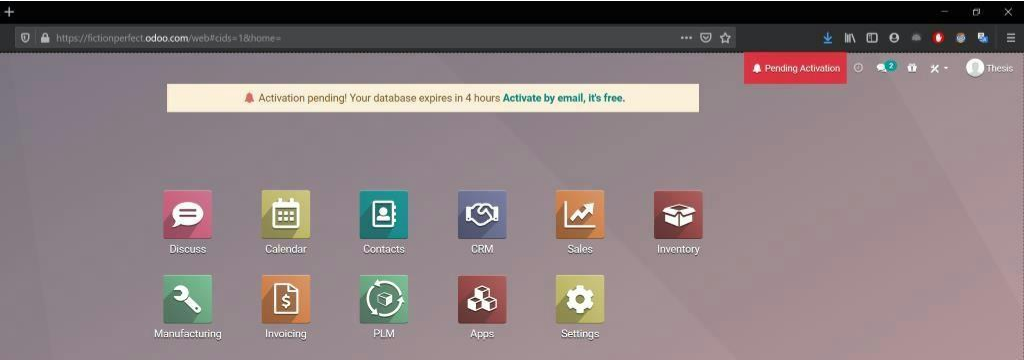
\includegraphics[width=441.9pt,height=155.0501pt]{latexImage_04781d280fc9249afbae6bab13a91597.png}}
\end{picture}
\newpage
\begin{tikzpicture}[overlay]\path(0pt,0pt);\end{tikzpicture}
\begin{picture}(-5,0)(2.5,0)
\put(500.14,-727.616){\fontsize{12}{1}\usefont{T1}{ptm}{m}{n}\selectfont\color{color_29791}27}
\put(512.14,-727.616){\fontsize{12}{1}\usefont{T1}{ptm}{m}{n}\selectfont\color{color_29791} }
\put(515.14,-727.616){\fontsize{12}{1}\usefont{T1}{ptm}{m}{n}\selectfont\color{color_29791} }
\put(70.104,-742.496){\fontsize{10.56}{1}\usefont{T1}{ptm}{m}{n}\selectfont\color{color_29791} }
\put(72.744,-742.496){\fontsize{12}{1}\usefont{T1}{ptm}{m}{n}\selectfont\color{color_29791} }
\put(82.944,-72.34003){\fontsize{12}{1}\usefont{T1}{ptm}{m}{n}\selectfont\color{color_29791}從}
\put(94.94,-72.34003){\fontsize{12}{1}\usefont{T1}{ptm}{m}{n}\selectfont\color{color_29791}Odoo}
\put(121.58,-72.34003){\fontsize{12}{1}\usefont{T1}{ptm}{m}{n}\selectfont\color{color_29791}的角度來看}
\put(181.61,-72.34003){\fontsize{12}{1}\usefont{T1}{ptm}{m}{n}\selectfont\color{color_29791},}
\put(193.61,-72.34003){\fontsize{12}{1}\usefont{T1}{ptm}{m}{n}\selectfont\color{color_29791}在任何常規製造過程的開始}
\put(337.63,-72.34003){\fontsize{12}{1}\usefont{T1}{ptm}{m}{n}\selectfont\color{color_29791},}
\put(349.63,-72.34003){\fontsize{12}{1}\usefont{T1}{ptm}{m}{n}\selectfont\color{color_29791}第一步將是工程師通常使用}
\put(493.66,-72.34003){\fontsize{12}{1}\usefont{T1}{ptm}{m}{n}\selectfont\color{color_29791}CA}
\put(69.384,-89.97998){\fontsize{12}{1}\usefont{T1}{ptm}{m}{n}\selectfont\color{color_29791}D}
\put(78.024,-89.97998){\fontsize{12}{1}\usefont{T1}{ptm}{m}{n}\selectfont\color{color_29791}軟體設計產品}
\put(150.02,-89.97998){\fontsize{12}{1}\usefont{T1}{ptm}{m}{n}\selectfont\color{color_29791}。}
\put(162.02,-89.97998){\fontsize{12}{1}\usefont{T1}{ptm}{m}{n}\selectfont\color{color_29791}完成後}
\put(198.05,-89.97998){\fontsize{12}{1}\usefont{T1}{ptm}{m}{n}\selectfont\color{color_29791},}
\put(210.05,-89.97998){\fontsize{12}{1}\usefont{T1}{ptm}{m}{n}\selectfont\color{color_29791}他們將創建物料清單}
\put(318.07,-89.97998){\fontsize{12}{1}\usefont{T1}{ptm}{m}{n}\selectfont\color{color_29791} }
\put(69.384,-107.62){\fontsize{12}{1}\usefont{T1}{ptm}{m}{n}\selectfont\color{color_29791}(}
\put(81.384,-107.62){\fontsize{12}{1}\usefont{T1}{ptm}{m}{n}\selectfont\color{color_29791}B}
\put(89.304,-107.62){\fontsize{12}{1}\usefont{T1}{ptm}{m}{n}\selectfont\color{color_29791}OM}
\put(108.62,-107.62){\fontsize{12}{1}\usefont{T1}{ptm}{m}{n}\selectfont\color{color_29791}),}
\put(132.62,-107.62){\fontsize{12}{1}\usefont{T1}{ptm}{m}{n}\selectfont\color{color_29791}這是生產}
\put(180.728,-107.62){\fontsize{12}{1}\usefont{T1}{ptm}{m}{n}\selectfont\color{color_29791}產品所需的元件或材料清單}
\put(324.79,-107.62){\fontsize{12}{1}\usefont{T1}{ptm}{m}{n}\selectfont\color{color_29791}。}
\put(336.79,-107.62){\fontsize{12}{1}\usefont{T1}{ptm}{m}{n}\selectfont\color{color_29791}在這一點上}
\put(396.79,-107.62){\fontsize{12}{1}\usefont{T1}{ptm}{m}{n}\selectfont\color{color_29791},}
\put(408.79,-107.62){\fontsize{12}{1}\usefont{T1}{ptm}{m}{n}\selectfont\color{color_29791}重點放在製造過程}
\put(69.384,-125.26){\fontsize{12}{1}\usefont{T1}{ptm}{m}{n}\selectfont\color{color_29791}本身}
\put(93.38,-125.26){\fontsize{12}{1}\usefont{T1}{ptm}{m}{n}\selectfont\color{color_29791}。}
\put(105.38,-125.26){\fontsize{12}{1}\usefont{T1}{ptm}{m}{n}\selectfont\color{color_29791}   }
\put(114.38,-125.26){\fontsize{12}{1}\usefont{T1}{ptm}{m}{n}\selectfont\color{color_29791} }
\put(84.264,-142.78){\fontsize{12}{1}\usefont{T1}{ptm}{m}{n}\selectfont\color{color_29791}  }
\put(90.26,-142.78){\fontsize{12}{1}\usefont{T1}{ptm}{m}{n}\selectfont\color{color_29791} }
\put(82.944,-158.74){\fontsize{12}{1}\usefont{T1}{ptm}{m}{n}\selectfont\color{color_29791}流程的軟體檢視側重於工藝路線}
\put(250.97,-158.74){\fontsize{12}{1}\usefont{T1}{ptm}{m}{n}\selectfont\color{color_29791}、}
\put(262.97,-158.74){\fontsize{12}{1}\usefont{T1}{ptm}{m}{n}\selectfont\color{color_29791}工作表和工作中心}
\put(358.99,-158.74){\fontsize{12}{1}\usefont{T1}{ptm}{m}{n}\selectfont\color{color_29791},}
\put(370.99,-158.74){\fontsize{12}{1}\usefont{T1}{ptm}{m}{n}\selectfont\color{color_29791}這是由製造工程團隊完成}
\put(69.384,-176.38){\fontsize{12}{1}\usefont{T1}{ptm}{m}{n}\selectfont\color{color_29791}的}
\put(81.384,-176.38){\fontsize{12}{1}\usefont{T1}{ptm}{m}{n}\selectfont\color{color_29791}。}
\put(93.38,-176.38){\fontsize{12}{1}\usefont{T1}{ptm}{m}{n}\selectfont\color{color_29791}工藝路線是產品在生產過程中經歷的一組步驟}
\put(333.43,-176.38){\fontsize{12}{1}\usefont{T1}{ptm}{m}{n}\selectfont\color{color_29791}。}
\put(345.43,-176.38){\fontsize{12}{1}\usefont{T1}{ptm}{m}{n}\selectfont\color{color_29791}工作表是製造操作員的指令}
\put(489.46,-176.38){\fontsize{12}{1}\usefont{T1}{ptm}{m}{n}\selectfont\color{color_29791},}
\put(69.384,-194.14){\fontsize{12}{1}\usefont{T1}{ptm}{m}{n}\selectfont\color{color_29791}工作中心是進行生產的地方}
\put(213.41,-194.14){\fontsize{12}{1}\usefont{T1}{ptm}{m}{n}\selectfont\color{color_29791}。}
\put(225.41,-194.14){\fontsize{12}{1}\usefont{T1}{ptm}{m}{n}\selectfont\color{color_29791}Odoo}
\put(252.05,-194.14){\fontsize{12}{1}\usefont{T1}{ptm}{m}{n}\selectfont\color{color_29791}認為這些是將工程師計劃付諸實施的要求}
\put(468.1,-194.14){\fontsize{12}{1}\usefont{T1}{ptm}{m}{n}\selectfont\color{color_29791}   }
\put(477.1,-194.14){\fontsize{12}{1}\usefont{T1}{ptm}{m}{n}\selectfont\color{color_29791} }
\put(84.264,-211.54){\fontsize{12}{1}\usefont{T1}{ptm}{m}{n}\selectfont\color{color_29791}  }
\put(90.26,-211.54){\fontsize{12}{1}\usefont{T1}{ptm}{m}{n}\selectfont\color{color_29791} }
\put(82.944,-227.5){\fontsize{12}{1}\usefont{T1}{ptm}{m}{n}\selectfont\color{color_29791}採購部門將負責詢價}
\put(190.97,-227.5){\fontsize{12}{1}\usefont{T1}{ptm}{m}{n}\selectfont\color{color_29791} }
\put(298.01,-227.5){\fontsize{12}{1}\usefont{T1}{ptm}{m}{n}\selectfont\color{color_29791}(}
\put(310.01,-227.5){\fontsize{12}{1}\usefont{T1}{ptm}{m}{n}\selectfont\color{color_29791}R}
\put(318.038,-227.5){\fontsize{12}{1}\usefont{T1}{ptm}{m}{n}\selectfont\color{color_29791}F}
\put(324.638,-227.5){\fontsize{12}{1}\usefont{T1}{ptm}{m}{n}\selectfont\color{color_29791}Q}
\put(333.31,-227.5){\fontsize{12}{1}\usefont{T1}{ptm}{m}{n}\selectfont\color{color_29791})}
\put(345.43,-227.5){\fontsize{12}{1}\usefont{T1}{ptm}{m}{n}\selectfont\color{color_29791} }
\put(452.5,-227.5){\fontsize{12}{1}\usefont{T1}{ptm}{m}{n}\selectfont\color{color_29791}或採購訂單}
\put(512.5,-227.5){\fontsize{12}{1}\usefont{T1}{ptm}{m}{n}\selectfont\color{color_29791} }
\put(69.384,-245.17){\fontsize{12}{1}\usefont{T1}{ptm}{m}{n}\selectfont\color{color_29791}(}
\put(81.384,-245.17){\fontsize{12}{1}\usefont{T1}{ptm}{m}{n}\selectfont\color{color_29791}PO}
\put(96.74,-245.17){\fontsize{12}{1}\usefont{T1}{ptm}{m}{n}\selectfont\color{color_29791})。}
\put(120.74,-245.17){\fontsize{12}{1}\usefont{T1}{ptm}{m}{n}\selectfont\color{color_29791}庫存操作員根據這些}
\put(228.77,-245.17){\fontsize{12}{1}\usefont{T1}{ptm}{m}{n}\selectfont\color{color_29791}採購訂單處理收據}
\put(324.79,-245.17){\fontsize{12}{1}\usefont{T1}{ptm}{m}{n}\selectfont\color{color_29791},}
\put(336.79,-245.17){\fontsize{12}{1}\usefont{T1}{ptm}{m}{n}\selectfont\color{color_29791}這通常是使用}
\put(408.79,-245.17){\fontsize{12}{1}\usefont{T1}{ptm}{m}{n}\selectfont\color{color_29791}Odoo}
\put(435.43,-245.17){\fontsize{12}{1}\usefont{T1}{ptm}{m}{n}\selectfont\color{color_29791}中的條碼應用}
\put(69.384,-262.81){\fontsize{12}{1}\usefont{T1}{ptm}{m}{n}\selectfont\color{color_29791}程式完成的}
\put(129.38,-262.81){\fontsize{12}{1}\usefont{T1}{ptm}{m}{n}\selectfont\color{color_29791}。}
\put(141.38,-262.81){\fontsize{12}{1}\usefont{T1}{ptm}{m}{n}\selectfont\color{color_29791}如本章第一節所述}
\put(237.41,-262.81){\fontsize{12}{1}\usefont{T1}{ptm}{m}{n}\selectfont\color{color_29791},}
\put(249.41,-262.81){\fontsize{12}{1}\usefont{T1}{ptm}{m}{n}\selectfont\color{color_29791}Odoo}
\put(276.05,-262.81){\fontsize{12}{1}\usefont{T1}{ptm}{m}{n}\selectfont\color{color_29791}主要是一個}
\put(336.07,-262.81){\fontsize{12}{1}\usefont{T1}{ptm}{m}{n}\selectfont\color{color_29791}ERP}
\put(358.15,-262.81){\fontsize{12}{1}\usefont{T1}{ptm}{m}{n}\selectfont\color{color_29791}系統}
\put(382.15,-262.81){\fontsize{12}{1}\usefont{T1}{ptm}{m}{n}\selectfont\color{color_29791},}
\put(394.15,-262.81){\fontsize{12}{1}\usefont{T1}{ptm}{m}{n}\selectfont\color{color_29791}在這一}
\put(430.03,-262.81){\fontsize{12}{1}\usefont{T1}{ptm}{m}{n}\selectfont\color{color_29791}點上}
\put(454.06,-262.81){\fontsize{12}{1}\usefont{T1}{ptm}{m}{n}\selectfont\color{color_29791},}
\put(466.06,-262.81){\fontsize{12}{1}\usefont{T1}{ptm}{m}{n}\selectfont\color{color_29791}可以注}
\put(69.384,-280.33){\fontsize{12}{1}\usefont{T1}{ptm}{m}{n}\selectfont\color{color_29791}意到一些以}
\put(129.38,-280.33){\fontsize{12}{1}\usefont{T1}{ptm}{m}{n}\selectfont\color{color_29791}ERP}
\put(151.46,-280.33){\fontsize{12}{1}\usefont{T1}{ptm}{m}{n}\selectfont\color{color_29791}為中心}
\put(187.34,-280.33){\fontsize{12}{1}\usefont{T1}{ptm}{m}{n}\selectfont\color{color_29791}的特徵}
\put(223.37,-280.33){\fontsize{12}{1}\usefont{T1}{ptm}{m}{n}\selectfont\color{color_29791},}
\put(235.37,-280.33){\fontsize{12}{1}\usefont{T1}{ptm}{m}{n}\selectfont\color{color_29791}例如對庫存和資源管理的關注}
\put(391.39,-280.33){\fontsize{12}{1}\usefont{T1}{ptm}{m}{n}\selectfont\color{color_29791}。}
\put(403.39,-280.33){\fontsize{12}{1}\usefont{T1}{ptm}{m}{n}\selectfont\color{color_29791}這將在以下各節中進}
\put(69.384,-298.09){\fontsize{12}{1}\usefont{T1}{ptm}{m}{n}\selectfont\color{color_29791}一步分析}
\put(117.38,-298.09){\fontsize{12}{1}\usefont{T1}{ptm}{m}{n}\selectfont\color{color_29791},}
\put(129.38,-298.09){\fontsize{12}{1}\usefont{T1}{ptm}{m}{n}\selectfont\color{color_29791}但公平地指出}
\put(201.41,-298.09){\fontsize{12}{1}\usefont{T1}{ptm}{m}{n}\selectfont\color{color_29791},}
\put(213.41,-298.09){\fontsize{12}{1}\usefont{T1}{ptm}{m}{n}\selectfont\color{color_29791}這些}
\put(237.41,-298.09){\fontsize{12}{1}\usefont{T1}{ptm}{m}{n}\selectfont\color{color_29791} }
\put(240.41,-298.09){\fontsize{12}{1}\usefont{T1}{ptm}{m}{n}\selectfont\color{color_29791}R}
\put(248.438,-298.09){\fontsize{12}{1}\usefont{T1}{ptm}{m}{n}\selectfont\color{color_29791}F}
\put(255.038,-298.09){\fontsize{12}{1}\usefont{T1}{ptm}{m}{n}\selectfont\color{color_29791}Q }
\put(266.69,-298.09){\fontsize{12}{1}\usefont{T1}{ptm}{m}{n}\selectfont\color{color_29791}和}
\put(278.69,-298.09){\fontsize{12}{1}\usefont{T1}{ptm}{m}{n}\selectfont\color{color_29791} }
\put(281.69,-298.09){\fontsize{12}{1}\usefont{T1}{ptm}{m}{n}\selectfont\color{color_29791}P}
\put(288.398,-298.09){\fontsize{12}{1}\usefont{T1}{ptm}{m}{n}\selectfont\color{color_29791}O }
\put(300.05,-298.09){\fontsize{12}{1}\usefont{T1}{ptm}{m}{n}\selectfont\color{color_29791}被視為資料庫中的專案}
\put(420.07,-298.09){\fontsize{12}{1}\usefont{T1}{ptm}{m}{n}\selectfont\color{color_29791}。}
\put(432.07,-298.09){\fontsize{12}{1}\usefont{T1}{ptm}{m}{n}\selectfont\color{color_29791}  }
\put(438.07,-298.09){\fontsize{12}{1}\usefont{T1}{ptm}{m}{n}\selectfont\color{color_29791} }
\put(84.264,-315.61){\fontsize{12}{1}\usefont{T1}{ptm}{m}{n}\selectfont\color{color_29791}   }
\put(93.26,-315.61){\fontsize{12}{1}\usefont{T1}{ptm}{m}{n}\selectfont\color{color_29791} }
\put(82.944,-331.57){\fontsize{12}{1}\usefont{T1}{ptm}{m}{n}\selectfont\color{color_29791}只有當您擁有所需的設計}
\put(214.97,-331.57){\fontsize{12}{1}\usefont{T1}{ptm}{m}{n}\selectfont\color{color_29791}、}
\put(226.97,-331.57){\fontsize{12}{1}\usefont{T1}{ptm}{m}{n}\selectfont\color{color_29791}工藝和材料時}
\put(298.97,-331.57){\fontsize{12}{1}\usefont{T1}{ptm}{m}{n}\selectfont\color{color_29791},}
\put(310.97,-331.57){\fontsize{12}{1}\usefont{T1}{ptm}{m}{n}\selectfont\color{color_29791}Odoo}
\put(337.63,-331.57){\fontsize{12}{1}\usefont{T1}{ptm}{m}{n}\selectfont\color{color_29791}才會考慮製造}
\put(409.63,-331.57){\fontsize{12}{1}\usefont{T1}{ptm}{m}{n}\selectfont\color{color_29791}。}
\put(421.63,-331.57){\fontsize{12}{1}\usefont{T1}{ptm}{m}{n}\selectfont\color{color_29791}然後}
\put(445.66,-331.57){\fontsize{12}{1}\usefont{T1}{ptm}{m}{n}\selectfont\color{color_29791},}
\put(457.66,-331.57){\fontsize{12}{1}\usefont{T1}{ptm}{m}{n}\selectfont\color{color_29791}製造領班}
\put(69.384,-349.21){\fontsize{12}{1}\usefont{T1}{ptm}{m}{n}\selectfont\color{color_29791}將創建製造訂單}
\put(153.38,-349.21){\fontsize{12}{1}\usefont{T1}{ptm}{m}{n}\selectfont\color{color_29791} }
\put(216.05,-349.21){\fontsize{12}{1}\usefont{T1}{ptm}{m}{n}\selectfont\color{color_29791}(}
\put(228.05,-349.21){\fontsize{12}{1}\usefont{T1}{ptm}{m}{n}\selectfont\color{color_29791}MO}
\put(247.37,-349.21){\fontsize{12}{1}\usefont{T1}{ptm}{m}{n}\selectfont\color{color_29791})}
\put(259.37,-349.21){\fontsize{12}{1}\usefont{T1}{ptm}{m}{n}\selectfont\color{color_29791} }
\put(322.03,-349.21){\fontsize{12}{1}\usefont{T1}{ptm}{m}{n}\selectfont\color{color_29791}並通過工作訂單}
\put(406.03,-349.21){\fontsize{12}{1}\usefont{T1}{ptm}{m}{n}\selectfont\color{color_29791} }
\put(468.7,-349.21){\fontsize{12}{1}\usefont{T1}{ptm}{m}{n}\selectfont\color{color_29791}(}
\put(480.7,-349.21){\fontsize{12}{1}\usefont{T1}{ptm}{m}{n}\selectfont\color{color_29791}WO}
\put(500.62,-349.21){\fontsize{12}{1}\usefont{T1}{ptm}{m}{n}\selectfont\color{color_29791})}
\put(512.5,-349.21){\fontsize{12}{1}\usefont{T1}{ptm}{m}{n}\selectfont\color{color_29791} }
\put(69.384,-366.73){\fontsize{12}{1}\usefont{T1}{ptm}{m}{n}\selectfont\color{color_29791}和工作中心管理製造操作員的計劃}
\put(249.41,-366.73){\fontsize{12}{1}\usefont{T1}{ptm}{m}{n}\selectfont\color{color_29791}。}
\put(261.41,-366.73){\fontsize{12}{1}\usefont{T1}{ptm}{m}{n}\selectfont\color{color_29791}然後}
\put(285.41,-366.73){\fontsize{12}{1}\usefont{T1}{ptm}{m}{n}\selectfont\color{color_29791},}
\put(297.41,-366.73){\fontsize{12}{1}\usefont{T1}{ptm}{m}{n}\selectfont\color{color_29791}製造操作員可以按照工作訂單開始生產}
\put(69.384,-384.37){\fontsize{12}{1}\usefont{T1}{ptm}{m}{n}\selectfont\color{color_29791}。}
\put(81.384,-384.37){\fontsize{12}{1}\usefont{T1}{ptm}{m}{n}\selectfont\color{color_29791}產品生產完成後}
\put(165.38,-384.37){\fontsize{12}{1}\usefont{T1}{ptm}{m}{n}\selectfont\color{color_29791},}
\put(177.38,-384.37){\fontsize{12}{1}\usefont{T1}{ptm}{m}{n}\selectfont\color{color_29791}它們會自}
\put(225.41,-384.37){\fontsize{12}{1}\usefont{T1}{ptm}{m}{n}\selectfont\color{color_29791}動出現在庫存資料庫中}
\put(345.43,-384.37){\fontsize{12}{1}\usefont{T1}{ptm}{m}{n}\selectfont\color{color_29791},}
\put(357.43,-384.37){\fontsize{12}{1}\usefont{T1}{ptm}{m}{n}\selectfont\color{color_29791}該資料庫與包裝和交付一起}
\put(69.384,-402.13){\fontsize{12}{1}\usefont{T1}{ptm}{m}{n}\selectfont\color{color_29791}由庫存部門管理}
\put(153.38,-402.13){\fontsize{12}{1}\usefont{T1}{ptm}{m}{n}\selectfont\color{color_29791}。}
\put(165.38,-402.13){\fontsize{12}{1}\usefont{T1}{ptm}{m}{n}\selectfont\color{color_29791}  }
\put(171.38,-402.13){\fontsize{12}{1}\usefont{T1}{ptm}{m}{n}\selectfont\color{color_29791} }
\put(84.264,-419.67){\fontsize{12}{1}\usefont{T1}{ptm}{m}{n}\selectfont\color{color_29791}   }
\put(93.26,-419.67){\fontsize{12}{1}\usefont{T1}{ptm}{m}{n}\selectfont\color{color_29791} }
\put(82.944,-435.51){\fontsize{12}{1}\usefont{T1}{ptm}{m}{n}\selectfont\color{color_29791}Odoo}
\put(109.58,-435.51){\fontsize{12}{1}\usefont{T1}{ptm}{m}{n}\selectfont\color{color_29791}認為質量團隊負責分配控制}
\put(253.61,-435.51){\fontsize{12}{1}\usefont{T1}{ptm}{m}{n}\selectfont\color{color_29791}/}
\put(256.97,-435.51){\fontsize{12}{1}\usefont{T1}{ptm}{m}{n}\selectfont\color{color_29791}檢查點}
\put(292.97,-435.51){\fontsize{12}{1}\usefont{T1}{ptm}{m}{n}\selectfont\color{color_29791},}
\put(304.97,-435.51){\fontsize{12}{1}\usefont{T1}{ptm}{m}{n}\selectfont\color{color_29791}並識別產品或生產中可能存在的問題}
\put(497.02,-435.51){\fontsize{12}{1}\usefont{T1}{ptm}{m}{n}\selectfont\color{color_29791}。}
\put(69.384,-453.15){\fontsize{12}{1}\usefont{T1}{ptm}{m}{n}\selectfont\color{color_29791}從}
\put(81.384,-453.15){\fontsize{12}{1}\usefont{T1}{ptm}{m}{n}\selectfont\color{color_29791}MES}
\put(106.1,-453.15){\fontsize{12}{1}\usefont{T1}{ptm}{m}{n}\selectfont\color{color_29791}的角度來看}
\put(166.1,-453.15){\fontsize{12}{1}\usefont{T1}{ptm}{m}{n}\selectfont\color{color_29791},}
\put(178.1,-453.15){\fontsize{12}{1}\usefont{T1}{ptm}{m}{n}\selectfont\color{color_29791}這些品質控制檢查點非常有趣}
\put(334.15,-453.15){\fontsize{12}{1}\usefont{T1}{ptm}{m}{n}\selectfont\color{color_29791},}
\put(346.15,-453.15){\fontsize{12}{1}\usefont{T1}{ptm}{m}{n}\selectfont\color{color_29791}因為它代表了在生產過程中即}
\put(69.384,-470.79){\fontsize{12}{1}\usefont{T1}{ptm}{m}{n}\selectfont\color{color_29791}時收集的有價值的生產數據}
\put(213.41,-470.79){\fontsize{12}{1}\usefont{T1}{ptm}{m}{n}\selectfont\color{color_29791},}
\put(225.41,-470.79){\fontsize{12}{1}\usefont{T1}{ptm}{m}{n}\selectfont\color{color_29791}即}
\put(237.41,-470.79){\fontsize{12}{1}\usefont{T1}{ptm}{m}{n}\selectfont\color{color_29791},}
\put(249.41,-470.79){\fontsize{12}{1}\usefont{T1}{ptm}{m}{n}\selectfont\color{color_29791}可以在每件作品生產後分配尺寸檢查}
\put(441.43,-470.79){\fontsize{12}{1}\usefont{T1}{ptm}{m}{n}\selectfont\color{color_29791},}
\put(453.46,-470.79){\fontsize{12}{1}\usefont{T1}{ptm}{m}{n}\selectfont\color{color_29791}機械師將}
\put(69.384,-488.55){\fontsize{12}{1}\usefont{T1}{ptm}{m}{n}\selectfont\color{color_29791}填寫尺寸以跟蹤品質隨時間推移}
\put(237.41,-488.55){\fontsize{12}{1}\usefont{T1}{ptm}{m}{n}\selectfont\color{color_29791}。}
\put(249.41,-488.55){\fontsize{12}{1}\usefont{T1}{ptm}{m}{n}\selectfont\color{color_29791}  }
\put(255.41,-488.55){\fontsize{12}{1}\usefont{T1}{ptm}{m}{n}\selectfont\color{color_29791} }
\put(84.264,-506.07){\fontsize{12}{1}\usefont{T1}{ptm}{m}{n}\selectfont\color{color_29791}  }
\put(90.26,-506.07){\fontsize{12}{1}\usefont{T1}{ptm}{m}{n}\selectfont\color{color_29791} }
\put(82.944,-521.91){\fontsize{12}{1}\usefont{T1}{ptm}{m}{n}\selectfont\color{color_29791}如果是設計問題或有改進的可能性}
\put(262.97,-521.91){\fontsize{12}{1}\usefont{T1}{ptm}{m}{n}\selectfont\color{color_29791},}
\put(274.97,-521.91){\fontsize{12}{1}\usefont{T1}{ptm}{m}{n}\selectfont\color{color_29791}可以發出工程變更單}
\put(382.99,-521.91){\fontsize{12}{1}\usefont{T1}{ptm}{m}{n}\selectfont\color{color_29791} }
\put(69.384,-539.55){\fontsize{12}{1}\usefont{T1}{ptm}{m}{n}\selectfont\color{color_29791}(}
\put(81.384,-539.55){\fontsize{12}{1}\usefont{T1}{ptm}{m}{n}\selectfont\color{color_29791}ECO}
\put(105.38,-539.55){\fontsize{12}{1}\usefont{T1}{ptm}{m}{n}\selectfont\color{color_29791})。}
\put(129.38,-539.55){\fontsize{12}{1}\usefont{T1}{ptm}{m}{n}\selectfont\color{color_29791}這又回到了製造工程團隊的手中}
\put(297.41,-539.55){\fontsize{12}{1}\usefont{T1}{ptm}{m}{n}\selectfont\color{color_29791},}
\put(309.41,-539.55){\fontsize{12}{1}\usefont{T1}{ptm}{m}{n}\selectfont\color{color_29791}並將專注於更新文檔和}
\put(429.43,-539.55){\fontsize{12}{1}\usefont{T1}{ptm}{m}{n}\selectfont\color{color_29791} }
\put(69.384,-557.19){\fontsize{12}{1}\usefont{T1}{ptm}{m}{n}\selectfont\color{color_29791}B}
\put(77.304,-557.19){\fontsize{12}{1}\usefont{T1}{ptm}{m}{n}\selectfont\color{color_29791}OM}
\put(96.62,-557.19){\fontsize{12}{1}\usefont{T1}{ptm}{m}{n}\selectfont\color{color_29791}。}
\put(108.62,-557.19){\fontsize{12}{1}\usefont{T1}{ptm}{m}{n}\selectfont\color{color_29791}ECO}
\put(132.62,-557.19){\fontsize{12}{1}\usefont{T1}{ptm}{m}{n}\selectfont\color{color_29791}是}
\put(144.62,-557.19){\fontsize{12}{1}\usefont{T1}{ptm}{m}{n}\selectfont\color{color_29791}Odoo}
\put(171.26,-557.19){\fontsize{12}{1}\usefont{T1}{ptm}{m}{n}\selectfont\color{color_29791}處}
\put(183.368,-557.19){\fontsize{12}{1}\usefont{T1}{ptm}{m}{n}\selectfont\color{color_29791}理系統內跟蹤變化的核心}
\put(315.43,-557.19){\fontsize{12}{1}\usefont{T1}{ptm}{m}{n}\selectfont\color{color_29791}。}
\put(327.43,-557.19){\fontsize{12}{1}\usefont{T1}{ptm}{m}{n}\selectfont\color{color_29791}在}
\put(339.43,-557.19){\fontsize{12}{1}\usefont{T1}{ptm}{m}{n}\selectfont\color{color_29791}PL}
\put(353.35,-557.19){\fontsize{12}{1}\usefont{T1}{ptm}{m}{n}\selectfont\color{color_29791}M}
\put(364.03,-557.19){\fontsize{12}{1}\usefont{T1}{ptm}{m}{n}\selectfont\color{color_29791}方面}
\put(388.03,-557.19){\fontsize{12}{1}\usefont{T1}{ptm}{m}{n}\selectfont\color{color_29791},}
\put(400.03,-557.19){\fontsize{12}{1}\usefont{T1}{ptm}{m}{n}\selectfont\color{color_29791}這是}
\put(424.138,-557.19){\fontsize{12}{1}\usefont{T1}{ptm}{m}{n}\selectfont\color{color_29791}關鍵}
\put(448.18,-557.19){\fontsize{12}{1}\usefont{T1}{ptm}{m}{n}\selectfont\color{color_29791},}
\put(460.18,-557.19){\fontsize{12}{1}\usefont{T1}{ptm}{m}{n}\selectfont\color{color_29791}事實上}
\put(496.18,-557.19){\fontsize{12}{1}\usefont{T1}{ptm}{m}{n}\selectfont\color{color_29791},}
\put(69.384,-574.83){\fontsize{12}{1}\usefont{T1}{ptm}{m}{n}\selectfont\color{color_29791}這是}
\put(93.62,-574.83){\fontsize{12}{1}\usefont{T1}{ptm}{m}{n}\selectfont\color{color_29791}O}
\put(102.368,-574.83){\fontsize{12}{1}\usefont{T1}{ptm}{m}{n}\selectfont\color{color_29791}d}
\put(108.476,-574.83){\fontsize{12}{1}\usefont{T1}{ptm}{m}{n}\selectfont\color{color_29791}o}
\put(114.584,-574.83){\fontsize{12}{1}\usefont{T1}{ptm}{m}{n}\selectfont\color{color_29791}o}
\put(120.74,-574.83){\fontsize{12}{1}\usefont{T1}{ptm}{m}{n}\selectfont\color{color_29791}應用程式}
\put(169.22,-574.83){\fontsize{12}{1}\usefont{T1}{ptm}{m}{n}\selectfont\color{color_29791}P}
\put(176.168,-574.83){\fontsize{12}{1}\usefont{T1}{ptm}{m}{n}\selectfont\color{color_29791}LM}
\put(194.33,-574.83){\fontsize{12}{1}\usefont{T1}{ptm}{m}{n}\selectfont\color{color_29791}的重點}
\put(230.69,-574.83){\fontsize{12}{1}\usefont{T1}{ptm}{m}{n}\selectfont\color{color_29791}。}
\put(242.93,-574.83){\fontsize{12}{1}\usefont{T1}{ptm}{m}{n}\selectfont\color{color_29791}所述應用程式能夠執行到什麼程度是下一節的主題}
\put(512.26,-574.83){\fontsize{12}{1}\usefont{T1}{ptm}{m}{n}\selectfont\color{color_29791}。}
\put(524.5,-574.83){\fontsize{12}{1}\usefont{T1}{ptm}{m}{n}\selectfont\color{color_29791}  }
\put(530.5,-574.83){\fontsize{12}{1}\usefont{T1}{ptm}{m}{n}\selectfont\color{color_29791} }
\put(105.38,-616.14){\fontsize{12.96}{1}\usefont{T1}{ptm}{b}{n}\selectfont\color{color_29791}5.1.3. Od}
\put(155.1723,-616.14){\fontsize{12.96}{1}\usefont{T1}{ptm}{b}{n}\selectfont\color{color_29791}oo}
\put(168.14,-616.14){\fontsize{12.96}{1}\usefont{T1}{ptm}{m}{n}\selectfont\color{color_29791}的}
\put(181.2037,-616.14){\fontsize{12.96}{1}\usefont{T1}{ptm}{m}{n}\selectfont\color{color_29791}信}
\put(194.2673,-616.14){\fontsize{12.96}{1}\usefont{T1}{ptm}{m}{n}\selectfont\color{color_29791}息}
\put(207.331,-616.14){\fontsize{12.96}{1}\usefont{T1}{ptm}{m}{n}\selectfont\color{color_29791}結構}
\put(233.45,-616.14){\fontsize{12.96}{1}\usefont{T1}{ptm}{b}{n}\selectfont\color{color_29791}  }
\put(239.93,-616.14){\fontsize{12.96}{1}\usefont{T1}{ptm}{b}{n}\selectfont\color{color_29791} }
\put(82.944,-645.18){\fontsize{12}{1}\usefont{T1}{ptm}{m}{n}\selectfont\color{color_29791}每個模組都側重於操作在資料庫中保存元數據的特定面向物件類}
\put(418.99,-645.18){\fontsize{12}{1}\usefont{T1}{ptm}{m}{n}\selectfont\color{color_29791}。}
\put(430.99,-645.18){\fontsize{12}{1}\usefont{T1}{ptm}{m}{n}\selectfont\color{color_29791}這些是負責虛}
\put(69.384,-662.82){\fontsize{12}{1}\usefont{T1}{ptm}{m}{n}\selectfont\color{color_29791}擬化產品生命週期各個方面的虛擬專案}
\put(273.41,-662.82){\fontsize{12}{1}\usefont{T1}{ptm}{m}{n}\selectfont\color{color_29791},}
\put(285.41,-662.82){\fontsize{12}{1}\usefont{T1}{ptm}{m}{n}\selectfont\color{color_29791}如}
\put(297.41,-662.82){\fontsize{12}{1}\usefont{T1}{ptm}{m}{n}\selectfont\color{color_29791}(}
\put(309.41,-662.82){\fontsize{12}{1}\usefont{T1}{ptm}{m}{n}\selectfont\color{color_29791}第}
\put(321.43,-662.82){\fontsize{12}{1}\usefont{T1}{ptm}{m}{n}\selectfont\color{color_29791}3.1}
\put(336.43,-662.82){\fontsize{12}{1}\usefont{T1}{ptm}{m}{n}\selectfont\color{color_29791}節}
\put(348.43,-662.82){\fontsize{12}{1}\usefont{T1}{ptm}{m}{n}\selectfont\color{color_29791})}
\put(360.43,-662.82){\fontsize{12}{1}\usefont{T1}{ptm}{m}{n}\selectfont\color{color_29791}中所述}
\put(396.43,-662.82){\fontsize{12}{1}\usefont{T1}{ptm}{m}{n}\selectfont\color{color_29791}。}
\put(408.43,-662.82){\fontsize{12}{1}\usefont{T1}{ptm}{m}{n}\selectfont\color{color_29791}不同類型的專案具}
\put(69.384,-680.34){\fontsize{12}{1}\usefont{T1}{ptm}{m}{n}\selectfont\color{color_29791}有不同類型的帳戶並持有不同類型的數據}
\put(285.41,-680.34){\fontsize{12}{1}\usefont{T1}{ptm}{m}{n}\selectfont\color{color_29791},}
\put(297.41,-680.34){\fontsize{12}{1}\usefont{T1}{ptm}{m}{n}\selectfont\color{color_29791}即產品專案代表特定產品}
\put(429.43,-680.34){\fontsize{12}{1}\usefont{T1}{ptm}{m}{n}\selectfont\color{color_29791},}
\put(441.43,-680.34){\fontsize{12}{1}\usefont{T1}{ptm}{m}{n}\selectfont\color{color_29791}並包含與其}
\put(69.384,-697.976){\fontsize{12}{1}\usefont{T1}{ptm}{m}{n}\selectfont\color{color_29791}交互和使用相關的元數據}
\put(201.41,-697.976){\fontsize{12}{1}\usefont{T1}{ptm}{m}{n}\selectfont\color{color_29791},}
\put(213.41,-697.976){\fontsize{12}{1}\usefont{T1}{ptm}{m}{n}\selectfont\color{color_29791}以及指向其他可能專案的連結}
\put(369.43,-697.976){\fontsize{12}{1}\usefont{T1}{ptm}{m}{n}\selectfont\color{color_29791},}
\put(381.43,-697.976){\fontsize{12}{1}\usefont{T1}{ptm}{m}{n}\selectfont\color{color_29791}這些專案密切相關}
\put(477.46,-697.976){\fontsize{12}{1}\usefont{T1}{ptm}{m}{n}\selectfont\color{color_29791},}
\put(489.46,-697.976){\fontsize{12}{1}\usefont{T1}{ptm}{m}{n}\selectfont\color{color_29791}例}
\end{picture}
\newpage
\begin{tikzpicture}[overlay]\path(0pt,0pt);\end{tikzpicture}
\begin{picture}(-5,0)(2.5,0)
\put(500.14,-727.616){\fontsize{12}{1}\usefont{T1}{ptm}{m}{n}\selectfont\color{color_29791}28}
\put(512.14,-727.616){\fontsize{12}{1}\usefont{T1}{ptm}{m}{n}\selectfont\color{color_29791} }
\put(515.14,-727.616){\fontsize{12}{1}\usefont{T1}{ptm}{m}{n}\selectfont\color{color_29791} }
\put(70.104,-742.496){\fontsize{10.56}{1}\usefont{T1}{ptm}{m}{n}\selectfont\color{color_29791} }
\put(72.744,-742.496){\fontsize{12}{1}\usefont{T1}{ptm}{m}{n}\selectfont\color{color_29791} }
\put(69.384,-72.34003){\fontsize{12}{1}\usefont{T1}{ptm}{m}{n}\selectfont\color{color_29791}如其責任使用者或製造所需的物料清單}
\put(273.41,-72.34003){\fontsize{12}{1}\usefont{T1}{ptm}{m}{n}\selectfont\color{color_29791}。}
\put(285.41,-72.34003){\fontsize{12}{1}\usefont{T1}{ptm}{m}{n}\selectfont\color{color_29791}Odoo}
\put(312.05,-72.34003){\fontsize{12}{1}\usefont{T1}{ptm}{m}{n}\selectfont\color{color_29791}使所有這些資訊都可以通過其瀏}
\put(480.1,-72.34003){\fontsize{12}{1}\usefont{T1}{ptm}{m}{n}\selectfont\color{color_29791}覽器}
\put(69.384,-89.97998){\fontsize{12}{1}\usefont{T1}{ptm}{m}{n}\selectfont\color{color_29791}介面訪問和交互}
\put(153.38,-89.97998){\fontsize{12}{1}\usefont{T1}{ptm}{m}{n}\selectfont\color{color_29791}(}
\put(165.38,-89.97998){\fontsize{12}{1}\usefont{T1}{ptm}{m}{n}\selectfont\color{color_29791}圖}
\put(177.38,-89.97998){\fontsize{12}{1}\usefont{T1}{ptm}{m}{n}\selectfont\color{color_29791}19}
\put(189.41,-89.97998){\fontsize{12}{1}\usefont{T1}{ptm}{m}{n}\selectfont\color{color_29791}和圖}
\put(213.41,-89.97998){\fontsize{12}{1}\usefont{T1}{ptm}{m}{n}\selectfont\color{color_29791}20}
\put(225.41,-89.97998){\fontsize{12}{1}\usefont{T1}{ptm}{m}{n}\selectfont\color{color_29791})。}
\put(249.41,-89.97998){\fontsize{12}{1}\usefont{T1}{ptm}{m}{n}\selectfont\color{color_29791}為了保持一致性}
\put(333.43,-89.97998){\fontsize{12}{1}\usefont{T1}{ptm}{m}{n}\selectfont\color{color_29791},}
\put(345.43,-89.97998){\fontsize{12}{1}\usefont{T1}{ptm}{m}{n}\selectfont\color{color_29791}本文檔將特定專案表示}
\put(465.46,-89.97998){\fontsize{12}{1}\usefont{T1}{ptm}{m}{n}\selectfont\color{color_29791}(}
\put(477.46,-89.97998){\fontsize{12}{1}\usefont{T1}{ptm}{m}{n}\selectfont\color{color_29791}例如}
\put(501.46,-89.97998){\fontsize{12}{1}\usefont{T1}{ptm}{m}{n}\selectfont\color{color_29791} }
\put(69.384,-107.74){\fontsize{12}{1}\usefont{T1}{ptm}{m}{n}\selectfont\color{color_29791}B}
\put(77.304,-107.74){\fontsize{12}{1}\usefont{T1}{ptm}{m}{n}\selectfont\color{color_29791}olt}
\put(90.02,-107.74){\fontsize{12}{1}\usefont{T1}{ptm}{m}{n}\selectfont\color{color_29791})}
\put(102.02,-107.74){\fontsize{12}{1}\usefont{T1}{ptm}{m}{n}\selectfont\color{color_29791}稱為}
\put(126.02,-107.74){\fontsize{12}{1}\usefont{T1}{ptm}{m}{n}\selectfont\color{color_29791}“}
\put(131.3,-107.74){\fontsize{12}{1}\usefont{T1}{ptm}{m}{n}\selectfont\color{color_29791}專案}
\put(155.3,-107.74){\fontsize{12}{1}\usefont{T1}{ptm}{m}{n}\selectfont\color{color_29791}”}
\put(160.58,-107.74){\fontsize{12}{1}\usefont{T1}{ptm}{m}{n}\selectfont\color{color_29791},}
\put(172.58,-107.74){\fontsize{12}{1}\usefont{T1}{ptm}{m}{n}\selectfont\color{color_29791}並}
\put(184.688,-107.74){\fontsize{12}{1}\usefont{T1}{ptm}{m}{n}\selectfont\color{color_29791}將專案類型}
\put(244.73,-107.74){\fontsize{12}{1}\usefont{T1}{ptm}{m}{n}\selectfont\color{color_29791}(}
\put(256.73,-107.74){\fontsize{12}{1}\usefont{T1}{ptm}{m}{n}\selectfont\color{color_29791}產品}
\put(280.73,-107.74){\fontsize{12}{1}\usefont{T1}{ptm}{m}{n}\selectfont\color{color_29791})}
\put(292.73,-107.74){\fontsize{12}{1}\usefont{T1}{ptm}{m}{n}\selectfont\color{color_29791}稱為}
\put(316.75,-107.74){\fontsize{12}{1}\usefont{T1}{ptm}{m}{n}\selectfont\color{color_29791}“}
\put(322.03,-107.74){\fontsize{12}{1}\usefont{T1}{ptm}{m}{n}\selectfont\color{color_29791}專案類}
\put(358.03,-107.74){\fontsize{12}{1}\usefont{T1}{ptm}{m}{n}\selectfont\color{color_29791}”}
\put(363.31,-107.74){\fontsize{12}{1}\usefont{T1}{ptm}{m}{n}\selectfont\color{color_29791}。}
\put(375.31,-107.74){\fontsize{12}{1}\usefont{T1}{ptm}{m}{n}\selectfont\color{color_29791} }
\put(378.43,-107.74){\fontsize{12}{1}\usefont{T1}{ptm}{m}{n}\selectfont\color{color_29791} }
\put(84.264,-125.14){\fontsize{12}{1}\usefont{T1}{ptm}{m}{n}\selectfont\color{color_29791} }
\put(87.26,-125.14){\fontsize{12}{1}\usefont{T1}{ptm}{m}{n}\selectfont\color{color_29791} }
\put(515.74,-417.51){\fontsize{12}{1}\usefont{T1}{ptm}{m}{n}\selectfont\color{color_29791} }
\put(518.74,-417.51){\fontsize{12}{1}\usefont{T1}{ptm}{m}{n}\selectfont\color{color_29791} }
\put(209.45,-440.07){\fontsize{12}{1}\usefont{T1}{ptm}{m}{n}\selectfont\color{color_29791}圖}
\put(221.57,-440.07){\fontsize{12}{1}\usefont{T1}{ptm}{b}{n}\selectfont\color{color_29791}19 }
\put(236.57,-440.07){\fontsize{12}{1}\usefont{T1}{ptm}{b}{n}\selectfont\color{color_29791}Od}
\put(252.638,-440.07){\fontsize{12}{1}\usefont{T1}{ptm}{b}{n}\selectfont\color{color_29791}oo}
\put(264.53,-440.07){\fontsize{12}{1}\usefont{T1}{ptm}{m}{n}\selectfont\color{color_29791}關於專案的介面示例}
\put(372.67,-440.07){\fontsize{12}{1}\usefont{T1}{ptm}{b}{n}\selectfont\color{color_29791} }
\put(375.55,-440.07){\fontsize{12}{1}\usefont{T1}{ptm}{m}{n}\selectfont\color{color_29791} }
\put(70.104,-456.63){\fontsize{12}{1}\usefont{T1}{ptm}{m}{n}\selectfont\color{color_29791} }
\put(73.104,-456.63){\fontsize{12}{1}\usefont{T1}{ptm}{m}{n}\selectfont\color{color_29791} }
\put(73.75,-417.42){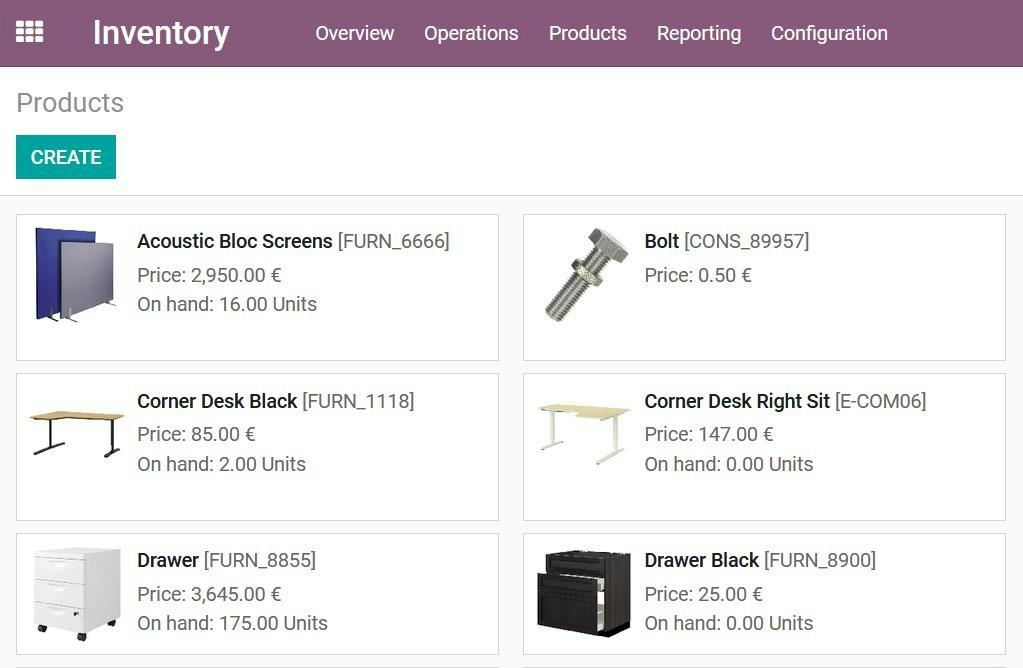
\includegraphics[width=441.9pt,height=288.55pt]{latexImage_6fe73730d3407d8491b9a1fe794808d5.png}}
\end{picture}
\newpage
\begin{tikzpicture}[overlay]\path(0pt,0pt);\end{tikzpicture}
\begin{picture}(-5,0)(2.5,0)
\put(500.14,-727.616){\fontsize{12}{1}\usefont{T1}{ptm}{m}{n}\selectfont\color{color_29791}29}
\put(512.14,-727.616){\fontsize{12}{1}\usefont{T1}{ptm}{m}{n}\selectfont\color{color_29791} }
\put(515.14,-727.616){\fontsize{12}{1}\usefont{T1}{ptm}{m}{n}\selectfont\color{color_29791} }
\put(70.104,-742.496){\fontsize{10.56}{1}\usefont{T1}{ptm}{m}{n}\selectfont\color{color_29791} }
\put(72.744,-742.496){\fontsize{12}{1}\usefont{T1}{ptm}{m}{n}\selectfont\color{color_29791} }
\put(515.74,-344.89){\fontsize{12}{1}\usefont{T1}{ptm}{m}{n}\selectfont\color{color_29791} }
\put(518.74,-344.89){\fontsize{12}{1}\usefont{T1}{ptm}{m}{n}\selectfont\color{color_29791} }
\put(181.97,-357.25){\fontsize{12}{1}\usefont{T1}{ptm}{m}{n}\selectfont\color{color_29791}圖}
\put(194.09,-357.25){\fontsize{12}{1}\usefont{T1}{ptm}{b}{n}\selectfont\color{color_29791}20 }
\put(209.09,-357.25){\fontsize{12}{1}\usefont{T1}{ptm}{b}{n}\selectfont\color{color_29791}G}
\put(218.33,-357.25){\fontsize{12}{1}\usefont{T1}{ptm}{b}{n}\selectfont\color{color_29791}UI}
\put(231.65,-357.25){\fontsize{12}{1}\usefont{T1}{ptm}{m}{n}\selectfont\color{color_29791}顯示的特}
\put(279.758,-357.25){\fontsize{12}{1}\usefont{T1}{ptm}{m}{n}\selectfont\color{color_29791}定專案及其元}
\put(351.866,-357.25){\fontsize{12}{1}\usefont{T1}{ptm}{m}{n}\selectfont\color{color_29791}數據示例}
\put(400.03,-357.25){\fontsize{12}{1}\usefont{T1}{ptm}{b}{n}\selectfont\color{color_29791} }
\put(402.91,-357.25){\fontsize{12}{1}\usefont{T1}{ptm}{m}{n}\selectfont\color{color_29791} }
\put(69.384,-385.09){\fontsize{12}{1}\usefont{T1}{ptm}{m}{n}\selectfont\color{color_29791}在}
\put(81.384,-385.09){\fontsize{12}{1}\usefont{T1}{ptm}{m}{n}\selectfont\color{color_29791}Odoo}
\put(108.02,-385.09){\fontsize{12}{1}\usefont{T1}{ptm}{m}{n}\selectfont\color{color_29791}中}
\put(120.02,-385.09){\fontsize{12}{1}\usefont{T1}{ptm}{m}{n}\selectfont\color{color_29791},}
\put(132.02,-385.09){\fontsize{12}{1}\usefont{T1}{ptm}{m}{n}\selectfont\color{color_29791}有幾種類型的專案類}
\put(240.05,-385.09){\fontsize{12}{1}\usefont{T1}{ptm}{m}{n}\selectfont\color{color_29791}(}
\put(252.05,-385.09){\fontsize{12}{1}\usefont{T1}{ptm}{m}{n}\selectfont\color{color_29791}有些包含大量元數據}
\put(360.07,-385.09){\fontsize{12}{1}\usefont{T1}{ptm}{m}{n}\selectfont\color{color_29791},}
\put(372.07,-385.09){\fontsize{12}{1}\usefont{T1}{ptm}{m}{n}\selectfont\color{color_29791}有些保存很少}
\put(444.07,-385.09){\fontsize{12}{1}\usefont{T1}{ptm}{m}{n}\selectfont\color{color_29791}),}
\put(468.1,-385.09){\fontsize{12}{1}\usefont{T1}{ptm}{m}{n}\selectfont\color{color_29791}它們都}
\put(69.384,-402.61){\fontsize{12}{1}\usefont{T1}{ptm}{m}{n}\selectfont\color{color_29791}具有不同程度的關係和集成}
\put(213.41,-402.61){\fontsize{12}{1}\usefont{T1}{ptm}{m}{n}\selectfont\color{color_29791}。}
\put(225.41,-402.61){\fontsize{12}{1}\usefont{T1}{ptm}{m}{n}\selectfont\color{color_29791}由於這項工作的範圍僅限於}
\put(369.43,-402.61){\fontsize{12}{1}\usefont{T1}{ptm}{m}{n}\selectfont\color{color_29791} }
\put(396.67,-402.61){\fontsize{12}{1}\usefont{T1}{ptm}{m}{n}\selectfont\color{color_29791}P}
\put(403.498,-402.61){\fontsize{12}{1}\usefont{T1}{ptm}{m}{n}\selectfont\color{color_29791}L}
\put(410.578,-402.61){\fontsize{12}{1}\usefont{T1}{ptm}{m}{n}\selectfont\color{color_29791}M}
\put(421.366,-402.61){\fontsize{12}{1}\usefont{T1}{ptm}{m}{n}\selectfont\color{color_29791} }
\put(448.66,-402.61){\fontsize{12}{1}\usefont{T1}{ptm}{m}{n}\selectfont\color{color_29791}和}
\put(460.66,-402.61){\fontsize{12}{1}\usefont{T1}{ptm}{m}{n}\selectfont\color{color_29791} }
\put(487.9,-402.61){\fontsize{12}{1}\usefont{T1}{ptm}{m}{n}\selectfont\color{color_29791}MES}
\put(512.5,-402.61){\fontsize{12}{1}\usefont{T1}{ptm}{m}{n}\selectfont\color{color_29791} }
\put(69.384,-420.27){\fontsize{12}{1}\usefont{T1}{ptm}{m}{n}\selectfont\color{color_29791}功能}
\put(93.38,-420.27){\fontsize{12}{1}\usefont{T1}{ptm}{m}{n}\selectfont\color{color_29791},}
\put(105.38,-420.27){\fontsize{12}{1}\usefont{T1}{ptm}{m}{n}\selectfont\color{color_29791}因此重點放在與之相關的專案上}
\put(273.41,-420.27){\fontsize{12}{1}\usefont{T1}{ptm}{m}{n}\selectfont\color{color_29791}。}
\put(285.41,-420.27){\fontsize{12}{1}\usefont{T1}{ptm}{m}{n}\selectfont\color{color_29791}以下各節將對}
\put(357.43,-420.27){\fontsize{12}{1}\usefont{T1}{ptm}{m}{n}\selectfont\color{color_29791}Odoo}
\put(384.07,-420.27){\fontsize{12}{1}\usefont{T1}{ptm}{m}{n}\selectfont\color{color_29791}製造過程的主要}
\put(468.1,-420.27){\fontsize{12}{1}\usefont{T1}{ptm}{m}{n}\selectfont\color{color_29791}7}
\put(474.1,-420.27){\fontsize{12}{1}\usefont{T1}{ptm}{m}{n}\selectfont\color{color_29791}個專案}
\put(69.384,-437.91){\fontsize{12}{1}\usefont{T1}{ptm}{m}{n}\selectfont\color{color_29791}類別進行簡短的解釋}
\put(177.38,-437.91){\fontsize{12}{1}\usefont{T1}{ptm}{m}{n}\selectfont\color{color_29791},}
\put(189.41,-437.91){\fontsize{12}{1}\usefont{T1}{ptm}{m}{n}\selectfont\color{color_29791}因為它的基本理解有助於讀者遵循類比}
\put(393.43,-437.91){\fontsize{12}{1}\usefont{T1}{ptm}{m}{n}\selectfont\color{color_29791}。}
\put(405.43,-437.91){\fontsize{12}{1}\usefont{T1}{ptm}{m}{n}\selectfont\color{color_29791}如下圖所示}
\put(465.46,-437.91){\fontsize{12}{1}\usefont{T1}{ptm}{m}{n}\selectfont\color{color_29791}(}
\put(477.46,-437.91){\fontsize{12}{1}\usefont{T1}{ptm}{m}{n}\selectfont\color{color_29791}圖}
\put(489.46,-437.91){\fontsize{12}{1}\usefont{T1}{ptm}{m}{n}\selectfont\color{color_29791} }
\put(69.384,-455.67){\fontsize{12}{1}\usefont{T1}{ptm}{m}{n}\selectfont\color{color_29791}21}
\put(81.384,-455.67){\fontsize{12}{1}\usefont{T1}{ptm}{m}{n}\selectfont\color{color_29791})。}
\put(105.38,-455.67){\fontsize{12}{1}\usefont{T1}{ptm}{m}{n}\selectfont\color{color_29791}製造過程外部的其他專案將在整個模擬過程中呈現}
\put(369.43,-455.67){\fontsize{12}{1}\usefont{T1}{ptm}{m}{n}\selectfont\color{color_29791}。}
\put(381.43,-455.67){\fontsize{12}{1}\usefont{T1}{ptm}{m}{n}\selectfont\color{color_29791} }
\put(384.43,-455.67){\fontsize{12}{1}\usefont{T1}{ptm}{m}{n}\selectfont\color{color_29791} }
\put(70.104,-473.19){\fontsize{12}{1}\usefont{T1}{ptm}{m}{n}\selectfont\color{color_29791} }
\put(73.104,-473.19){\fontsize{12}{1}\usefont{T1}{ptm}{m}{n}\selectfont\color{color_29791} }
\put(73.75,-344.75){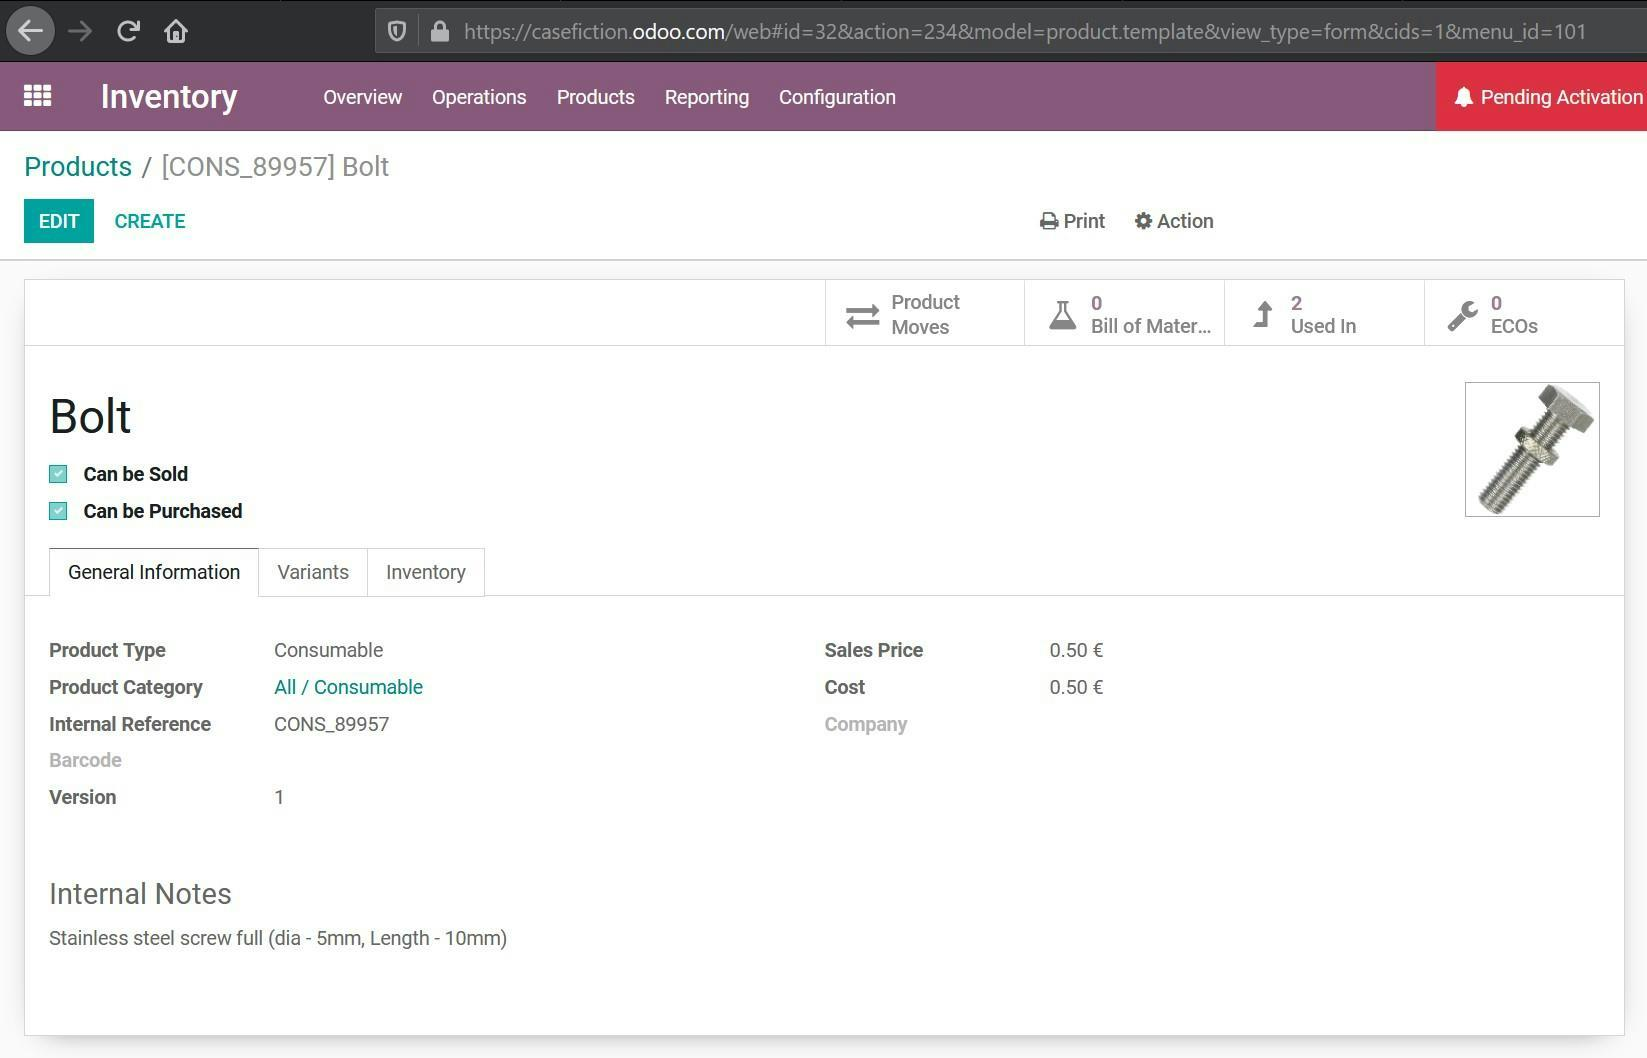
\includegraphics[width=441.9pt,height=283.85pt]{latexImage_27869fb065f6dc419a262c5ad541823e.png}}
\end{picture}
\newpage
\begin{tikzpicture}[overlay]\path(0pt,0pt);\end{tikzpicture}
\begin{picture}(-5,0)(2.5,0)
\put(500.14,-727.616){\fontsize{12}{1}\usefont{T1}{ptm}{m}{n}\selectfont\color{color_29791}30}
\put(512.14,-727.616){\fontsize{12}{1}\usefont{T1}{ptm}{m}{n}\selectfont\color{color_29791} }
\put(515.14,-727.616){\fontsize{12}{1}\usefont{T1}{ptm}{m}{n}\selectfont\color{color_29791} }
\put(70.104,-742.496){\fontsize{10.56}{1}\usefont{T1}{ptm}{m}{n}\selectfont\color{color_29791} }
\put(72.744,-742.496){\fontsize{12}{1}\usefont{T1}{ptm}{m}{n}\selectfont\color{color_29791} }
\put(529.9,-534.63){\fontsize{12}{1}\usefont{T1}{ptm}{m}{n}\selectfont\color{color_29791} }
\put(532.9,-534.63){\fontsize{12}{1}\usefont{T1}{ptm}{m}{n}\selectfont\color{color_29791} }
\put(86.06,-557.31){\fontsize{12}{1}\usefont{T1}{ptm}{m}{n}\selectfont\color{color_29791}圖}
\put(98.18,-557.31){\fontsize{12}{1}\usefont{T1}{ptm}{b}{n}\selectfont\color{color_29791} }
\put(101.18,-557.31){\fontsize{12}{1}\usefont{T1}{ptm}{b}{n}\selectfont\color{color_29791}21 }
\put(116.06,-557.31){\fontsize{12}{1}\usefont{T1}{ptm}{m}{n}\selectfont\color{color_29791}簡化物}
\put(152.168,-557.31){\fontsize{12}{1}\usefont{T1}{ptm}{m}{n}\selectfont\color{color_29791}料與產品製造的關}
\put(248.276,-557.31){\fontsize{12}{1}\usefont{T1}{ptm}{m}{n}\selectfont\color{color_29791}係圖}
\put(272.45,-557.31){\fontsize{12}{1}\usefont{T1}{ptm}{b}{n}\selectfont\color{color_29791} }
\put(275.45,-557.31){\fontsize{12}{1}\usefont{T1}{ptm}{b}{n}\selectfont\color{color_29791}X }
\put(286.97,-557.31){\fontsize{12}{1}\usefont{T1}{ptm}{m}{n}\selectfont\color{color_29791} }
\put(70.104,-574.59){\fontsize{12}{1}\usefont{T1}{ptm}{m}{n}\selectfont\color{color_29791} }
\put(73.104,-574.59){\fontsize{12}{1}\usefont{T1}{ptm}{m}{n}\selectfont\color{color_29791} }
\put(70.104,-611.22){\fontsize{11.04}{1}\usefont{T1}{ptm}{m}{n}\selectfont\color{color_29791} }
\put(124.1,-611.22){\fontsize{12}{1}\usefont{T1}{ptm}{b}{n}\selectfont\color{color_29791}5.1.3.1. }
\put(163.1,-611.22){\fontsize{12}{1}\usefont{T1}{ptm}{b}{n}\selectfont\color{color_29791} }
\put(188.21,-611.22){\fontsize{12}{1}\usefont{T1}{ptm}{m}{n}\selectfont\color{color_29791}產品專案}
\put(236.33,-611.22){\fontsize{12}{1}\usefont{T1}{ptm}{b}{n}\selectfont\color{color_29791}  }
\put(242.21,-611.22){\fontsize{12}{1}\usefont{T1}{ptm}{m}{n}\selectfont\color{color_29791} }
\put(82.944,-641.34){\fontsize{12}{1}\usefont{T1}{ptm}{m}{n}\selectfont\color{color_29791}每種材料}
\put(130.94,-641.34){\fontsize{12}{1}\usefont{T1}{ptm}{m}{n}\selectfont\color{color_29791}、}
\put(142.94,-641.34){\fontsize{12}{1}\usefont{T1}{ptm}{m}{n}\selectfont\color{color_29791}元件或產品都以產品類型類為特徵}
\put(322.99,-641.34){\fontsize{12}{1}\usefont{T1}{ptm}{m}{n}\selectfont\color{color_29791},}
\put(334.99,-641.34){\fontsize{12}{1}\usefont{T1}{ptm}{m}{n}\selectfont\color{color_29791}該類主要在}
\put(394.99,-641.34){\fontsize{12}{1}\usefont{T1}{ptm}{m}{n}\selectfont\color{color_29791}Odoo}
\put(421.63,-641.34){\fontsize{12}{1}\usefont{T1}{ptm}{m}{n}\selectfont\color{color_29791}的}
\put(433.63,-641.34){\fontsize{12}{1}\usefont{T1}{ptm}{m}{n}\selectfont\color{color_29791}庫存應用程式}
\put(69.384,-658.86){\fontsize{12}{1}\usefont{T1}{ptm}{m}{n}\selectfont\color{color_29791}中保存和管理}
\put(141.38,-658.86){\fontsize{12}{1}\usefont{T1}{ptm}{m}{n}\selectfont\color{color_29791}。}
\put(153.38,-658.86){\fontsize{12}{1}\usefont{T1}{ptm}{m}{n}\selectfont\color{color_29791}這意味著}
\put(201.41,-658.86){\fontsize{12}{1}\usefont{T1}{ptm}{m}{n}\selectfont\color{color_29791},}
\put(213.41,-658.86){\fontsize{12}{1}\usefont{T1}{ptm}{m}{n}\selectfont\color{color_29791}在系統內}
\put(261.41,-658.86){\fontsize{12}{1}\usefont{T1}{ptm}{m}{n}\selectfont\color{color_29791},}
\put(273.41,-658.86){\fontsize{12}{1}\usefont{T1}{ptm}{m}{n}\selectfont\color{color_29791}產品生產取決於其他產品的可用性}
\put(453.46,-658.86){\fontsize{12}{1}\usefont{T1}{ptm}{m}{n}\selectfont\color{color_29791},}
\put(465.46,-658.86){\fontsize{12}{1}\usefont{T1}{ptm}{m}{n}\selectfont\color{color_29791}這些產}
\put(69.384,-676.5){\fontsize{12}{1}\usefont{T1}{ptm}{m}{n}\selectfont\color{color_29791}品要麼按原樣購買}
\put(165.38,-676.5){\fontsize{12}{1}\usefont{T1}{ptm}{m}{n}\selectfont\color{color_29791},}
\put(177.38,-676.5){\fontsize{12}{1}\usefont{T1}{ptm}{m}{n}\selectfont\color{color_29791}要麼從其他產品製造}
\put(285.41,-676.5){\fontsize{12}{1}\usefont{T1}{ptm}{m}{n}\selectfont\color{color_29791}(}
\put(297.41,-676.5){\fontsize{12}{1}\usefont{T1}{ptm}{m}{n}\selectfont\color{color_29791}圖}
\put(309.41,-676.5){\fontsize{12}{1}\usefont{T1}{ptm}{m}{n}\selectfont\color{color_29791}22}
\put(321.43,-676.5){\fontsize{12}{1}\usefont{T1}{ptm}{m}{n}\selectfont\color{color_29791}),}
\put(345.43,-676.5){\fontsize{12}{1}\usefont{T1}{ptm}{m}{n}\selectfont\color{color_29791}即原材料也被視為產品}
\put(465.46,-676.5){\fontsize{12}{1}\usefont{T1}{ptm}{m}{n}\selectfont\color{color_29791},}
\put(477.46,-676.5){\fontsize{12}{1}\usefont{T1}{ptm}{m}{n}\selectfont\color{color_29791}更具}
\put(87.9,-534.5){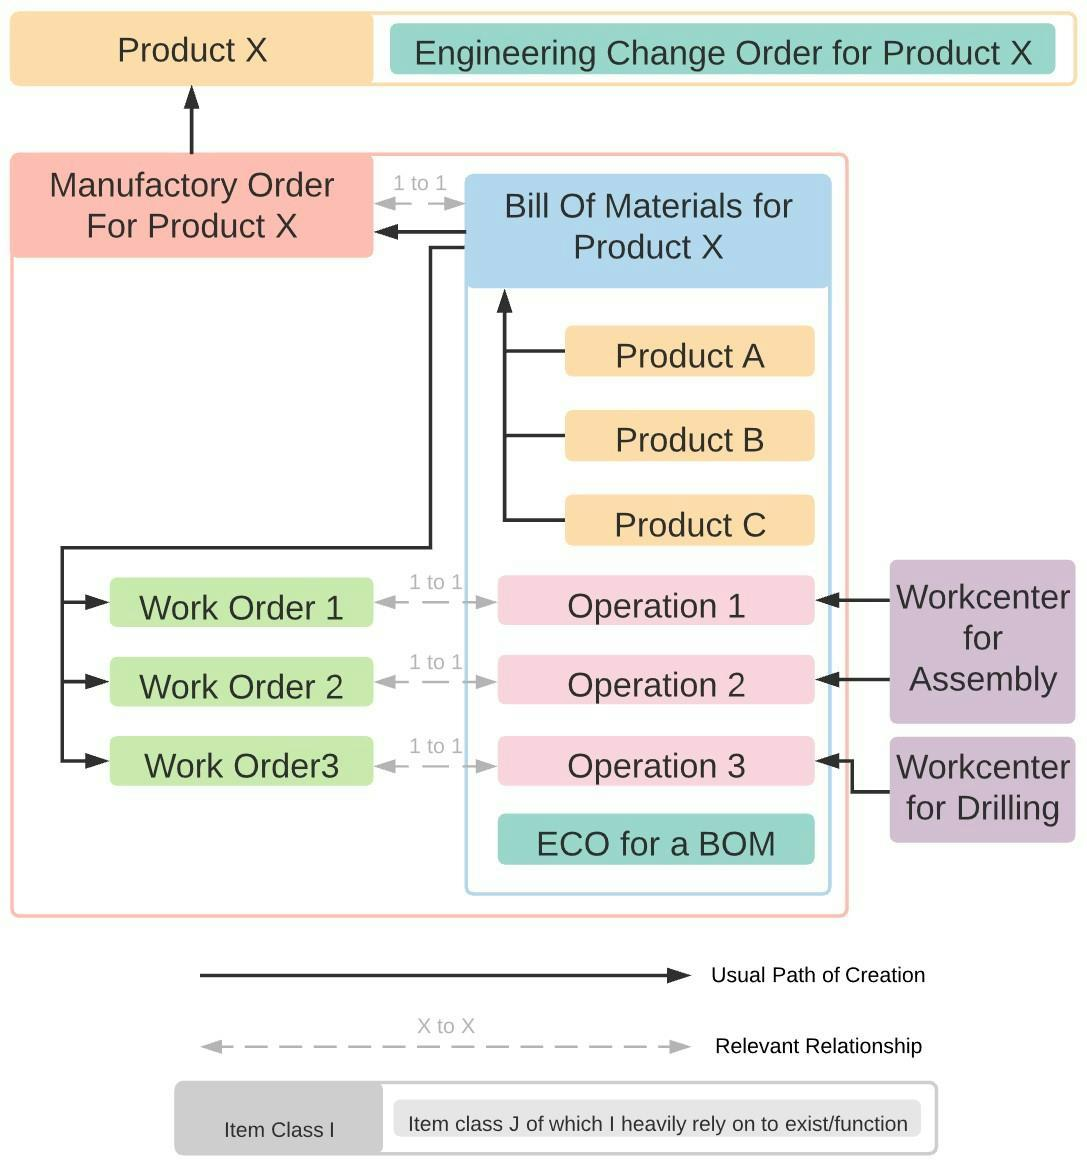
\includegraphics[width=441.9pt,height=473.6pt]{latexImage_149602aa69f10993700a4609ab74c728.png}}
\end{picture}
\newpage
\begin{tikzpicture}[overlay]\path(0pt,0pt);\end{tikzpicture}
\begin{picture}(-5,0)(2.5,0)
\put(500.14,-727.616){\fontsize{12}{1}\usefont{T1}{ptm}{m}{n}\selectfont\color{color_29791}31}
\put(512.14,-727.616){\fontsize{12}{1}\usefont{T1}{ptm}{m}{n}\selectfont\color{color_29791} }
\put(515.14,-727.616){\fontsize{12}{1}\usefont{T1}{ptm}{m}{n}\selectfont\color{color_29791} }
\put(70.104,-742.496){\fontsize{10.56}{1}\usefont{T1}{ptm}{m}{n}\selectfont\color{color_29791} }
\put(72.744,-742.496){\fontsize{12}{1}\usefont{T1}{ptm}{m}{n}\selectfont\color{color_29791} }
\put(69.384,-72.34003){\fontsize{12}{1}\usefont{T1}{ptm}{m}{n}\selectfont\color{color_29791}體地說}
\put(105.38,-72.34003){\fontsize{12}{1}\usefont{T1}{ptm}{m}{n}\selectfont\color{color_29791},}
\put(117.38,-72.34003){\fontsize{12}{1}\usefont{T1}{ptm}{m}{n}\selectfont\color{color_29791}是購買的產品}
\put(189.41,-72.34003){\fontsize{12}{1}\usefont{T1}{ptm}{m}{n}\selectfont\color{color_29791},}
\put(201.41,-72.34003){\fontsize{12}{1}\usefont{T1}{ptm}{m}{n}\selectfont\color{color_29791}然後包含在}
\put(261.41,-72.34003){\fontsize{12}{1}\usefont{T1}{ptm}{m}{n}\selectfont\color{color_29791}B}
\put(269.33,-72.34003){\fontsize{12}{1}\usefont{T1}{ptm}{m}{n}\selectfont\color{color_29791}OM}
\put(288.65,-72.34003){\fontsize{12}{1}\usefont{T1}{ptm}{m}{n}\selectfont\color{color_29791}中}
\put(300.758,-72.34003){\fontsize{12}{1}\usefont{T1}{ptm}{m}{n}\selectfont\color{color_29791}以製造其他產品}
\put(384.79,-72.34003){\fontsize{12}{1}\usefont{T1}{ptm}{m}{n}\selectfont\color{color_29791}。}
\put(396.79,-72.34003){\fontsize{12}{1}\usefont{T1}{ptm}{m}{n}\selectfont\color{color_29791}這被認為是主要專案}
\put(69.384,-90.09998){\fontsize{12}{1}\usefont{T1}{ptm}{m}{n}\selectfont\color{color_29791}類}
\put(81.384,-90.09998){\fontsize{12}{1}\usefont{T1}{ptm}{m}{n}\selectfont\color{color_29791},}
\put(93.38,-90.09998){\fontsize{12}{1}\usefont{T1}{ptm}{m}{n}\selectfont\color{color_29791}因為它既是製造的來源}
\put(213.41,-90.09998){\fontsize{12}{1}\usefont{T1}{ptm}{m}{n}\selectfont\color{color_29791},}
\put(225.41,-90.09998){\fontsize{12}{1}\usefont{T1}{ptm}{m}{n}\selectfont\color{color_29791}也是製造的目標}
\put(309.41,-90.09998){\fontsize{12}{1}\usefont{T1}{ptm}{m}{n}\selectfont\color{color_29791}。}
\put(321.43,-90.09998){\fontsize{12}{1}\usefont{T1}{ptm}{m}{n}\selectfont\color{color_29791}  }
\put(327.43,-90.09998){\fontsize{12}{1}\usefont{T1}{ptm}{m}{n}\selectfont\color{color_29791} }
\put(84.264,-107.5){\fontsize{12}{1}\usefont{T1}{ptm}{m}{n}\selectfont\color{color_29791} }
\put(87.26,-107.5){\fontsize{12}{1}\usefont{T1}{ptm}{m}{n}\selectfont\color{color_29791} }
\put(473.02,-221.38){\fontsize{12}{1}\usefont{T1}{ptm}{m}{n}\selectfont\color{color_29791} }
\put(476.02,-221.38){\fontsize{12}{1}\usefont{T1}{ptm}{m}{n}\selectfont\color{color_29791} }
\put(236.81,-233.86){\fontsize{12}{1}\usefont{T1}{ptm}{m}{n}\selectfont\color{color_29791}圖}
\put(248.93,-233.86){\fontsize{12}{1}\usefont{T1}{ptm}{b}{n}\selectfont\color{color_29791}22}
\put(260.81,-233.86){\fontsize{12}{1}\usefont{T1}{ptm}{m}{n}\selectfont\color{color_29791}簡化產}
\put(296.918,-233.86){\fontsize{12}{1}\usefont{T1}{ptm}{m}{n}\selectfont\color{color_29791}品關係圖}
\put(345.07,-233.86){\fontsize{12}{1}\usefont{T1}{ptm}{b}{n}\selectfont\color{color_29791} }
\put(347.95,-233.86){\fontsize{12}{1}\usefont{T1}{ptm}{m}{n}\selectfont\color{color_29791} }
\put(70.104,-272.29){\fontsize{11.04}{1}\usefont{T1}{ptm}{m}{n}\selectfont\color{color_29791} }
\put(124.1,-272.29){\fontsize{12}{1}\usefont{T1}{ptm}{b}{n}\selectfont\color{color_29791}5.1.3.2. }
\put(163.1,-272.29){\fontsize{12}{1}\usefont{T1}{ptm}{b}{n}\selectfont\color{color_29791} }
\put(220.97,-272.29){\fontsize{12}{1}\usefont{T1}{ptm}{m}{n}\selectfont\color{color_29791}工序物料}
\put(269.078,-272.29){\fontsize{12}{1}\usefont{T1}{ptm}{m}{n}\selectfont\color{color_29791}類和工作中心物料類}
\put(377.23,-272.29){\fontsize{12}{1}\usefont{T1}{ptm}{b}{n}\selectfont\color{color_29791} }
\put(380.11,-272.29){\fontsize{12}{1}\usefont{T1}{ptm}{m}{n}\selectfont\color{color_29791} }
\put(82.944,-302.29){\fontsize{12}{1}\usefont{T1}{ptm}{m}{n}\selectfont\color{color_29791}工序專案代表將元件或原材料轉化為產品或新元件所需的製造工序}
\put(430.99,-302.29){\fontsize{12}{1}\usefont{T1}{ptm}{m}{n}\selectfont\color{color_29791},}
\put(442.99,-302.29){\fontsize{12}{1}\usefont{T1}{ptm}{m}{n}\selectfont\color{color_29791}而工作中心}
\put(69.384,-319.93){\fontsize{12}{1}\usefont{T1}{ptm}{m}{n}\selectfont\color{color_29791}專案則代表工序發生的地方}
\put(213.41,-319.93){\fontsize{12}{1}\usefont{T1}{ptm}{m}{n}\selectfont\color{color_29791},}
\put(225.41,-319.93){\fontsize{12}{1}\usefont{T1}{ptm}{m}{n}\selectfont\color{color_29791}例如}
\put(249.41,-319.93){\fontsize{12}{1}\usefont{T1}{ptm}{m}{n}\selectfont\color{color_29791},}
\put(261.41,-319.93){\fontsize{12}{1}\usefont{T1}{ptm}{m}{n}\selectfont\color{color_29791}在具有適當設備的砂光站}
\put(393.43,-319.93){\fontsize{12}{1}\usefont{T1}{ptm}{m}{n}\selectfont\color{color_29791}(}
\put(405.43,-319.93){\fontsize{12}{1}\usefont{T1}{ptm}{m}{n}\selectfont\color{color_29791}圖}
\put(417.43,-319.93){\fontsize{12}{1}\usefont{T1}{ptm}{m}{n}\selectfont\color{color_29791} }
\put(69.384,-337.57){\fontsize{12}{1}\usefont{T1}{ptm}{m}{n}\selectfont\color{color_29791}23}
\put(81.384,-337.57){\fontsize{12}{1}\usefont{T1}{ptm}{m}{n}\selectfont\color{color_29791})}
\put(93.38,-337.57){\fontsize{12}{1}\usefont{T1}{ptm}{m}{n}\selectfont\color{color_29791}中進行打磨木材}
\put(177.38,-337.57){\fontsize{12}{1}\usefont{T1}{ptm}{m}{n}\selectfont\color{color_29791}。}
\put(189.41,-337.57){\fontsize{12}{1}\usefont{T1}{ptm}{m}{n}\selectfont\color{color_29791}該工作中心最終在}
\put(285.41,-337.57){\fontsize{12}{1}\usefont{T1}{ptm}{m}{n}\selectfont\color{color_29791}Odoo}
\put(312.05,-337.57){\fontsize{12}{1}\usefont{T1}{ptm}{m}{n}\selectfont\color{color_29791}中用作其生產計劃中的時間}
\put(456.1,-337.57){\fontsize{12}{1}\usefont{T1}{ptm}{m}{n}\selectfont\color{color_29791}/}
\put(459.46,-337.57){\fontsize{12}{1}\usefont{T1}{ptm}{m}{n}\selectfont\color{color_29791}設備管理}
\put(69.384,-355.21){\fontsize{12}{1}\usefont{T1}{ptm}{m}{n}\selectfont\color{color_29791}工具}
\put(93.38,-355.21){\fontsize{12}{1}\usefont{T1}{ptm}{m}{n}\selectfont\color{color_29791}。}
\put(105.38,-355.21){\fontsize{12}{1}\usefont{T1}{ptm}{m}{n}\selectfont\color{color_29791}基本上}
\put(141.38,-355.21){\fontsize{12}{1}\usefont{T1}{ptm}{m}{n}\selectfont\color{color_29791},}
\put(153.38,-355.21){\fontsize{12}{1}\usefont{T1}{ptm}{m}{n}\selectfont\color{color_29791}當生產中心滿負荷運轉時}
\put(285.41,-355.21){\fontsize{12}{1}\usefont{T1}{ptm}{m}{n}\selectfont\color{color_29791},}
\put(297.41,-355.21){\fontsize{12}{1}\usefont{T1}{ptm}{m}{n}\selectfont\color{color_29791}它會暫停後續流程或將流程重定向到備}
\put(69.384,-372.85){\fontsize{12}{1}\usefont{T1}{ptm}{m}{n}\selectfont\color{color_29791}用工作中心}
\put(129.38,-372.85){\fontsize{12}{1}\usefont{T1}{ptm}{m}{n}\selectfont\color{color_29791}。}
\put(141.38,-372.85){\fontsize{12}{1}\usefont{T1}{ptm}{m}{n}\selectfont\color{color_29791}操作項還負責保存生產過程中查閱的指令檔}
\put(369.43,-372.85){\fontsize{12}{1}\usefont{T1}{ptm}{m}{n}\selectfont\color{color_29791}。}
\put(381.43,-372.85){\fontsize{12}{1}\usefont{T1}{ptm}{m}{n}\selectfont\color{color_29791}  }
\put(387.43,-372.85){\fontsize{12}{1}\usefont{T1}{ptm}{m}{n}\selectfont\color{color_29791} }
\put(70.104,-390.37){\fontsize{12}{1}\usefont{T1}{ptm}{m}{n}\selectfont\color{color_29791} }
\put(73.104,-390.37){\fontsize{12}{1}\usefont{T1}{ptm}{m}{n}\selectfont\color{color_29791} }
\put(515.74,-514.59){\fontsize{12}{1}\usefont{T1}{ptm}{m}{n}\selectfont\color{color_29791} }
\put(518.74,-514.59){\fontsize{12}{1}\usefont{T1}{ptm}{m}{n}\selectfont\color{color_29791} }
\put(248.93,-527.07){\fontsize{12}{1}\usefont{T1}{ptm}{m}{n}\selectfont\color{color_29791}圖}
\put(261.05,-527.07){\fontsize{12}{1}\usefont{T1}{ptm}{b}{n}\selectfont\color{color_29791}23}
\put(272.93,-527.07){\fontsize{12}{1}\usefont{T1}{ptm}{m}{n}\selectfont\color{color_29791}簡化操}
\put(309.038,-527.07){\fontsize{12}{1}\usefont{T1}{ptm}{m}{n}\selectfont\color{color_29791}作圖}
\put(333.19,-527.07){\fontsize{12}{1}\usefont{T1}{ptm}{b}{n}\selectfont\color{color_29791} }
\put(336.07,-527.07){\fontsize{12}{1}\usefont{T1}{ptm}{m}{n}\selectfont\color{color_29791} }
\put(70.104,-544.47){\fontsize{12}{1}\usefont{T1}{ptm}{m}{n}\selectfont\color{color_29791} }
\put(73.104,-544.47){\fontsize{12}{1}\usefont{T1}{ptm}{m}{n}\selectfont\color{color_29791} }
\put(70.104,-583.11){\fontsize{11.04}{1}\usefont{T1}{ptm}{m}{n}\selectfont\color{color_29791} }
\put(124.1,-583.11){\fontsize{12}{1}\usefont{T1}{ptm}{b}{n}\selectfont\color{color_29791}5.1.3.3. }
\put(163.1,-583.11){\fontsize{12}{1}\usefont{T1}{ptm}{b}{n}\selectfont\color{color_29791} }
\put(221.57,-583.11){\fontsize{12}{1}\usefont{T1}{ptm}{m}{n}\selectfont\color{color_29791}物料清單}
\put(269.678,-583.11){\fontsize{12}{1}\usefont{T1}{ptm}{m}{n}\selectfont\color{color_29791}項類}
\put(293.81,-583.11){\fontsize{12}{1}\usefont{T1}{ptm}{b}{n}\selectfont\color{color_29791} }
\put(296.69,-583.11){\fontsize{12}{1}\usefont{T1}{ptm}{m}{n}\selectfont\color{color_29791} }
\put(82.944,-613.14){\fontsize{12}{1}\usefont{T1}{ptm}{m}{n}\selectfont\color{color_29791}物料清單是構建產品所需的元件清單}
\put(274.97,-613.14){\fontsize{12}{1}\usefont{T1}{ptm}{m}{n}\selectfont\color{color_29791}。}
\put(286.97,-613.14){\fontsize{12}{1}\usefont{T1}{ptm}{m}{n}\selectfont\color{color_29791}然而}
\put(310.97,-613.14){\fontsize{12}{1}\usefont{T1}{ptm}{m}{n}\selectfont\color{color_29791},}
\put(322.99,-613.14){\fontsize{12}{1}\usefont{T1}{ptm}{m}{n}\selectfont\color{color_29791}在}
\put(334.99,-613.14){\fontsize{12}{1}\usefont{T1}{ptm}{m}{n}\selectfont\color{color_29791}Odoo}
\put(361.63,-613.14){\fontsize{12}{1}\usefont{T1}{ptm}{m}{n}\selectfont\color{color_29791}中}
\put(373.63,-613.14){\fontsize{12}{1}\usefont{T1}{ptm}{m}{n}\selectfont\color{color_29791},}
\put(385.63,-613.14){\fontsize{12}{1}\usefont{T1}{ptm}{m}{n}\selectfont\color{color_29791}B}
\put(393.55,-613.14){\fontsize{12}{1}\usefont{T1}{ptm}{m}{n}\selectfont\color{color_29791}OM}
\put(412.87,-613.14){\fontsize{12}{1}\usefont{T1}{ptm}{m}{n}\selectfont\color{color_29791}最好}
\put(436.978,-613.14){\fontsize{12}{1}\usefont{T1}{ptm}{m}{n}\selectfont\color{color_29791}用}
\put(449.02,-613.14){\fontsize{12}{1}\usefont{T1}{ptm}{m}{n}\selectfont\color{color_29791}P}
\put(455.848,-613.14){\fontsize{12}{1}\usefont{T1}{ptm}{m}{n}\selectfont\color{color_29791}L}
\put(462.928,-613.14){\fontsize{12}{1}\usefont{T1}{ptm}{m}{n}\selectfont\color{color_29791}M}
\put(473.62,-613.14){\fontsize{12}{1}\usefont{T1}{ptm}{m}{n}\selectfont\color{color_29791}認為生}
\put(69.384,-630.78){\fontsize{12}{1}\usefont{T1}{ptm}{m}{n}\selectfont\color{color_29791}產過程的虛擬表示來描述}
\put(201.41,-630.78){\fontsize{12}{1}\usefont{T1}{ptm}{m}{n}\selectfont\color{color_29791}。}
\put(213.41,-630.78){\fontsize{12}{1}\usefont{T1}{ptm}{m}{n}\selectfont\color{color_29791}考慮到前面提到的工序物料類}
\put(369.43,-630.78){\fontsize{12}{1}\usefont{T1}{ptm}{m}{n}\selectfont\color{color_29791},}
\put(381.43,-630.78){\fontsize{12}{1}\usefont{T1}{ptm}{m}{n}\selectfont\color{color_29791}乍一看似乎有悖常理}
\put(489.46,-630.78){\fontsize{12}{1}\usefont{T1}{ptm}{m}{n}\selectfont\color{color_29791},}
\put(69.384,-648.42){\fontsize{12}{1}\usefont{T1}{ptm}{m}{n}\selectfont\color{color_29791}但實際上}
\put(117.38,-648.42){\fontsize{12}{1}\usefont{T1}{ptm}{m}{n}\selectfont\color{color_29791},}
\put(129.38,-648.42){\fontsize{12}{1}\usefont{T1}{ptm}{m}{n}\selectfont\color{color_29791}由於物料清單是複合物料}
\put(261.41,-648.42){\fontsize{12}{1}\usefont{T1}{ptm}{m}{n}\selectfont\color{color_29791},}
\put(273.41,-648.42){\fontsize{12}{1}\usefont{T1}{ptm}{m}{n}\selectfont\color{color_29791}它直接指向生產最終產品所需的所有物料類}
\put(69.384,-666.06){\fontsize{12}{1}\usefont{T1}{ptm}{m}{n}\selectfont\color{color_29791}型}
\put(81.384,-666.06){\fontsize{12}{1}\usefont{T1}{ptm}{m}{n}\selectfont\color{color_29791}(}
\put(93.38,-666.06){\fontsize{12}{1}\usefont{T1}{ptm}{m}{n}\selectfont\color{color_29791}圖}
\put(105.38,-666.06){\fontsize{12}{1}\usefont{T1}{ptm}{m}{n}\selectfont\color{color_29791} }
\put(129.14,-666.06){\fontsize{12}{1}\usefont{T1}{ptm}{m}{n}\selectfont\color{color_29791}24}
\put(141.14,-666.06){\fontsize{12}{1}\usefont{T1}{ptm}{m}{n}\selectfont\color{color_29791})。}
\put(165.14,-666.06){\fontsize{12}{1}\usefont{T1}{ptm}{m}{n}\selectfont\color{color_29791}例如}
\put(189.17,-666.06){\fontsize{12}{1}\usefont{T1}{ptm}{m}{n}\selectfont\color{color_29791},}
\put(201.17,-666.06){\fontsize{12}{1}\usefont{T1}{ptm}{m}{n}\selectfont\color{color_29791}假設要構建一個產品}
\put(309.17,-666.06){\fontsize{12}{1}\usefont{T1}{ptm}{m}{n}\selectfont\color{color_29791},}
\put(321.19,-666.06){\fontsize{12}{1}\usefont{T1}{ptm}{m}{n}\selectfont\color{color_29791}需要}
\put(345.19,-666.06){\fontsize{12}{1}\usefont{T1}{ptm}{m}{n}\selectfont\color{color_29791} }
\put(368.95,-666.06){\fontsize{12}{1}\usefont{T1}{ptm}{m}{n}\selectfont\color{color_29791}3 }
\put(398.71,-666.06){\fontsize{12}{1}\usefont{T1}{ptm}{m}{n}\selectfont\color{color_29791}個不同的部件和}
\put(482.74,-666.06){\fontsize{12}{1}\usefont{T1}{ptm}{m}{n}\selectfont\color{color_29791} }
\put(506.5,-666.06){\fontsize{12}{1}\usefont{T1}{ptm}{m}{n}\selectfont\color{color_29791}4 }
\put(69.384,-683.816){\fontsize{12}{1}\usefont{T1}{ptm}{m}{n}\selectfont\color{color_29791}個不同的操作}
\put(141.38,-683.816){\fontsize{12}{1}\usefont{T1}{ptm}{m}{n}\selectfont\color{color_29791};}
\put(144.74,-683.816){\fontsize{12}{1}\usefont{T1}{ptm}{m}{n}\selectfont\color{color_29791}所述產品的}
\put(204.77,-683.816){\fontsize{12}{1}\usefont{T1}{ptm}{m}{n}\selectfont\color{color_29791}B}
\put(212.69,-683.816){\fontsize{12}{1}\usefont{T1}{ptm}{m}{n}\selectfont\color{color_29791}OM}
\put(232.01,-683.816){\fontsize{12}{1}\usefont{T1}{ptm}{m}{n}\selectfont\color{color_29791}將列出所有}
\put(292.118,-683.816){\fontsize{12}{1}\usefont{T1}{ptm}{m}{n}\selectfont\color{color_29791}這些產品}
\put(340.15,-683.816){\fontsize{12}{1}\usefont{T1}{ptm}{m}{n}\selectfont\color{color_29791},}
\put(352.15,-683.816){\fontsize{12}{1}\usefont{T1}{ptm}{m}{n}\selectfont\color{color_29791}並指定它們的使用順序}
\put(472.18,-683.816){\fontsize{12}{1}\usefont{T1}{ptm}{m}{n}\selectfont\color{color_29791}。}
\put(484.18,-683.816){\fontsize{12}{1}\usefont{T1}{ptm}{m}{n}\selectfont\color{color_29791}  }
\put(490.18,-683.816){\fontsize{12}{1}\usefont{T1}{ptm}{m}{n}\selectfont\color{color_29791} }
\put(70.104,-701.216){\fontsize{12}{1}\usefont{T1}{ptm}{m}{n}\selectfont\color{color_29791} }
\put(73.104,-701.216){\fontsize{12}{1}\usefont{T1}{ptm}{m}{n}\selectfont\color{color_29791} }
\put(130,-221.39){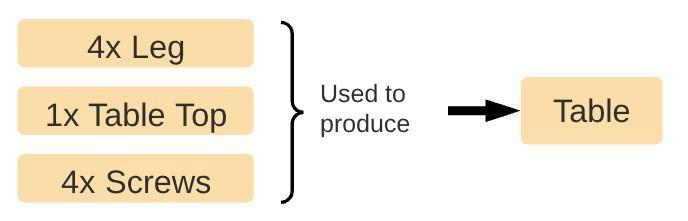
\includegraphics[width=342.9pt,height=110.15pt]{latexImage_4abb17474f661045a2f698acbfb6b184.png}}
\put(73.75,-514.55){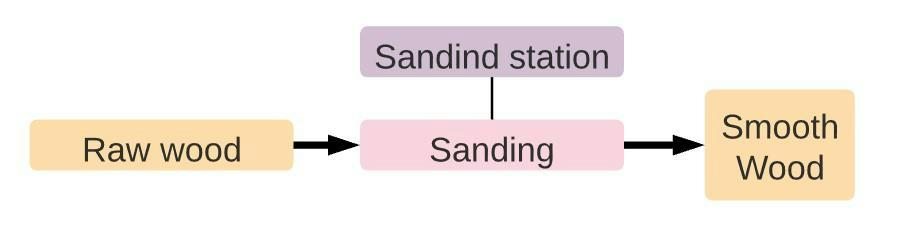
\includegraphics[width=441.9pt,height=120.5pt]{latexImage_39d6395d61bcde1a5bb345fd1f10f01f.png}}
\end{picture}
\newpage
\begin{tikzpicture}[overlay]\path(0pt,0pt);\end{tikzpicture}
\begin{picture}(-5,0)(2.5,0)
\put(500.14,-727.616){\fontsize{12}{1}\usefont{T1}{ptm}{m}{n}\selectfont\color{color_29791}32}
\put(512.14,-727.616){\fontsize{12}{1}\usefont{T1}{ptm}{m}{n}\selectfont\color{color_29791} }
\put(515.14,-727.616){\fontsize{12}{1}\usefont{T1}{ptm}{m}{n}\selectfont\color{color_29791} }
\put(70.104,-742.496){\fontsize{10.56}{1}\usefont{T1}{ptm}{m}{n}\selectfont\color{color_29791} }
\put(72.744,-742.496){\fontsize{12}{1}\usefont{T1}{ptm}{m}{n}\selectfont\color{color_29791} }
\put(515.74,-433.35){\fontsize{12}{1}\usefont{T1}{ptm}{m}{n}\selectfont\color{color_29791} }
\put(518.74,-433.35){\fontsize{12}{1}\usefont{T1}{ptm}{m}{n}\selectfont\color{color_29791} }
\put(234.65,-445.83){\fontsize{12}{1}\usefont{T1}{ptm}{m}{n}\selectfont\color{color_29791}圖}
\put(246.77,-445.83){\fontsize{12}{1}\usefont{T1}{ptm}{b}{n}\selectfont\color{color_29791} }
\put(249.77,-445.83){\fontsize{12}{1}\usefont{T1}{ptm}{b}{n}\selectfont\color{color_29791}24 }
\put(264.65,-445.83){\fontsize{12}{1}\usefont{T1}{ptm}{m}{n}\selectfont\color{color_29791}簡化的}
\put(300.77,-445.83){\fontsize{12}{1}\usefont{T1}{ptm}{b}{n}\selectfont\color{color_29791} }
\put(303.77,-445.83){\fontsize{12}{1}\usefont{T1}{ptm}{b}{n}\selectfont\color{color_29791}B}
\put(311.798,-445.83){\fontsize{12}{1}\usefont{T1}{ptm}{b}{n}\selectfont\color{color_29791}OM }
\put(335.35,-445.83){\fontsize{12}{1}\usefont{T1}{ptm}{m}{n}\selectfont\color{color_29791}圖}
\put(347.47,-445.83){\fontsize{12}{1}\usefont{T1}{ptm}{b}{n}\selectfont\color{color_29791} }
\put(350.35,-445.83){\fontsize{12}{1}\usefont{T1}{ptm}{m}{n}\selectfont\color{color_29791} }
\put(70.104,-484.23){\fontsize{11.04}{1}\usefont{T1}{ptm}{m}{n}\selectfont\color{color_29791} }
\put(124.1,-484.23){\fontsize{12}{1}\usefont{T1}{ptm}{b}{n}\selectfont\color{color_29791}5.1.3.4. }
\put(163.1,-484.23){\fontsize{12}{1}\usefont{T1}{ptm}{b}{n}\selectfont\color{color_29791} }
\put(249.41,-484.23){\fontsize{12}{1}\usefont{T1}{ptm}{m}{n}\selectfont\color{color_29791}製造訂單}
\put(297.518,-484.23){\fontsize{12}{1}\usefont{T1}{ptm}{m}{n}\selectfont\color{color_29791}項類和工作訂單項類}
\put(405.67,-484.23){\fontsize{12}{1}\usefont{T1}{ptm}{b}{n}\selectfont\color{color_29791}  }
\put(411.55,-484.23){\fontsize{12}{1}\usefont{T1}{ptm}{m}{n}\selectfont\color{color_29791} }
\put(82.944,-514.23){\fontsize{12}{1}\usefont{T1}{ptm}{m}{n}\selectfont\color{color_29791}在}
\put(94.94,-514.23){\fontsize{12}{1}\usefont{T1}{ptm}{m}{n}\selectfont\color{color_29791}Odoo}
\put(121.58,-514.23){\fontsize{12}{1}\usefont{T1}{ptm}{m}{n}\selectfont\color{color_29791}中考慮的標準專案中}
\put(229.61,-514.23){\fontsize{12}{1}\usefont{T1}{ptm}{m}{n}\selectfont\color{color_29791},}
\put(241.61,-514.23){\fontsize{12}{1}\usefont{T1}{ptm}{m}{n}\selectfont\color{color_29791}訂單是代表系統}
\put(325.63,-514.23){\fontsize{12}{1}\usefont{T1}{ptm}{m}{n}\selectfont\color{color_29791}內開始的訂單}
\put(397.63,-514.23){\fontsize{12}{1}\usefont{T1}{ptm}{m}{n}\selectfont\color{color_29791}。}
\put(409.63,-514.23){\fontsize{12}{1}\usefont{T1}{ptm}{m}{n}\selectfont\color{color_29791}他們發出信號}
\put(481.66,-514.23){\fontsize{12}{1}\usefont{T1}{ptm}{m}{n}\selectfont\color{color_29791},}
\put(493.66,-514.23){\fontsize{12}{1}\usefont{T1}{ptm}{m}{n}\selectfont\color{color_29791}表}
\put(69.384,-531.87){\fontsize{12}{1}\usefont{T1}{ptm}{m}{n}\selectfont\color{color_29791}明正在以某種方式和某個地方發生變化}
\put(273.41,-531.87){\fontsize{12}{1}\usefont{T1}{ptm}{m}{n}\selectfont\color{color_29791}。}
\put(285.41,-531.87){\fontsize{12}{1}\usefont{T1}{ptm}{m}{n}\selectfont\color{color_29791}對於製造訂單}
\put(357.43,-531.87){\fontsize{12}{1}\usefont{T1}{ptm}{m}{n}\selectfont\color{color_29791},}
\put(369.43,-531.87){\fontsize{12}{1}\usefont{T1}{ptm}{m}{n}\selectfont\color{color_29791}它表示使用其物料清單作}
\put(69.384,-549.51){\fontsize{12}{1}\usefont{T1}{ptm}{m}{n}\selectfont\color{color_29791}為基礎製造}
\put(129.38,-549.51){\fontsize{12}{1}\usefont{T1}{ptm}{m}{n}\selectfont\color{color_29791} }
\put(503.86,-549.51){\fontsize{12}{1}\usefont{T1}{ptm}{m}{n}\selectfont\color{color_29791}N }
\put(69.384,-567.03){\fontsize{12}{1}\usefont{T1}{ptm}{m}{n}\selectfont\color{color_29791}個特定產品的訂單}
\put(165.38,-567.03){\fontsize{12}{1}\usefont{T1}{ptm}{m}{n}\selectfont\color{color_29791}。}
\put(177.38,-567.03){\fontsize{12}{1}\usefont{T1}{ptm}{m}{n}\selectfont\color{color_29791}正是由於該}
\put(237.41,-567.03){\fontsize{12}{1}\usefont{T1}{ptm}{m}{n}\selectfont\color{color_29791}MO}
\put(256.73,-567.03){\fontsize{12}{1}\usefont{T1}{ptm}{m}{n}\selectfont\color{color_29791},}
\put(268.73,-567.03){\fontsize{12}{1}\usefont{T1}{ptm}{m}{n}\selectfont\color{color_29791}Odoo}
\put(295.37,-567.03){\fontsize{12}{1}\usefont{T1}{ptm}{m}{n}\selectfont\color{color_29791}會自動生成工單}
\put(379.39,-567.03){\fontsize{12}{1}\usefont{T1}{ptm}{m}{n}\selectfont\color{color_29791}(}
\put(391.39,-567.03){\fontsize{12}{1}\usefont{T1}{ptm}{m}{n}\selectfont\color{color_29791}B}
\put(399.31,-567.03){\fontsize{12}{1}\usefont{T1}{ptm}{m}{n}\selectfont\color{color_29791}OM}
\put(418.75,-567.03){\fontsize{12}{1}\usefont{T1}{ptm}{m}{n}\selectfont\color{color_29791}中列出的每個必}
\put(69.384,-584.79){\fontsize{12}{1}\usefont{T1}{ptm}{m}{n}\selectfont\color{color_29791}要操作一個}
\put(129.38,-584.79){\fontsize{12}{1}\usefont{T1}{ptm}{m}{n}\selectfont\color{color_29791}),}
\put(153.38,-584.79){\fontsize{12}{1}\usefont{T1}{ptm}{m}{n}\selectfont\color{color_29791}並在整個可用的必要工作中心分配}
\put(333.43,-584.79){\fontsize{12}{1}\usefont{T1}{ptm}{m}{n}\selectfont\color{color_29791}(}
\put(345.43,-584.79){\fontsize{12}{1}\usefont{T1}{ptm}{m}{n}\selectfont\color{color_29791}圖}
\put(357.43,-584.79){\fontsize{12}{1}\usefont{T1}{ptm}{m}{n}\selectfont\color{color_29791}25}
\put(369.43,-584.79){\fontsize{12}{1}\usefont{T1}{ptm}{m}{n}\selectfont\color{color_29791})。}
\put(393.43,-584.79){\fontsize{12}{1}\usefont{T1}{ptm}{m}{n}\selectfont\color{color_29791}  }
\put(399.43,-584.79){\fontsize{12}{1}\usefont{T1}{ptm}{m}{n}\selectfont\color{color_29791} }
\put(84.264,-602.34){\fontsize{12}{1}\usefont{T1}{ptm}{m}{n}\selectfont\color{color_29791} }
\put(87.26,-602.34){\fontsize{12}{1}\usefont{T1}{ptm}{m}{n}\selectfont\color{color_29791} }
\put(82.944,-617.46){\fontsize{12}{1}\usefont{T1}{ptm}{m}{n}\selectfont\color{color_29791}工單是製造操作員與}
\put(190.97,-617.46){\fontsize{12}{1}\usefont{T1}{ptm}{m}{n}\selectfont\color{color_29791}Odoo}
\put(217.61,-617.46){\fontsize{12}{1}\usefont{T1}{ptm}{m}{n}\selectfont\color{color_29791}交互的主要形式}
\put(301.61,-617.46){\fontsize{12}{1}\usefont{T1}{ptm}{m}{n}\selectfont\color{color_29791},}
\put(313.63,-617.46){\fontsize{12}{1}\usefont{T1}{ptm}{m}{n}\selectfont\color{color_29791}它呈現操作項指定的所有指令}
\put(469.66,-617.46){\fontsize{12}{1}\usefont{T1}{ptm}{m}{n}\selectfont\color{color_29791},}
\put(481.66,-617.46){\fontsize{12}{1}\usefont{T1}{ptm}{m}{n}\selectfont\color{color_29791}以及}
\put(69.384,-635.1){\fontsize{12}{1}\usefont{T1}{ptm}{m}{n}\selectfont\color{color_29791}對其完成的控制}
\put(153.38,-635.1){\fontsize{12}{1}\usefont{T1}{ptm}{m}{n}\selectfont\color{color_29791}。}
\put(165.38,-635.1){\fontsize{12}{1}\usefont{T1}{ptm}{m}{n}\selectfont\color{color_29791}當}
\put(177.38,-635.1){\fontsize{12}{1}\usefont{T1}{ptm}{m}{n}\selectfont\color{color_29791} }
\put(492.58,-635.1){\fontsize{12}{1}\usefont{T1}{ptm}{m}{n}\selectfont\color{color_29791}W}
\put(503.968,-635.1){\fontsize{12}{1}\usefont{T1}{ptm}{m}{n}\selectfont\color{color_29791}O}
\put(512.488,-635.1){\fontsize{12}{1}\usefont{T1}{ptm}{m}{n}\selectfont\color{color_29791} }
\put(69.384,-652.74){\fontsize{12}{1}\usefont{T1}{ptm}{m}{n}\selectfont\color{color_29791}發生時}
\put(105.38,-652.74){\fontsize{12}{1}\usefont{T1}{ptm}{m}{n}\selectfont\color{color_29791},}
\put(117.38,-652.74){\fontsize{12}{1}\usefont{T1}{ptm}{m}{n}\selectfont\color{color_29791}操作員通過介面發出信號}
\put(249.41,-652.74){\fontsize{12}{1}\usefont{T1}{ptm}{m}{n}\selectfont\color{color_29791},}
\put(261.41,-652.74){\fontsize{12}{1}\usefont{T1}{ptm}{m}{n}\selectfont\color{color_29791}發出信號}
\put(309.41,-652.74){\fontsize{12}{1}\usefont{T1}{ptm}{m}{n}\selectfont\color{color_29791},}
\put(321.43,-652.74){\fontsize{12}{1}\usefont{T1}{ptm}{m}{n}\selectfont\color{color_29791}發出信號}
\put(369.43,-652.74){\fontsize{12}{1}\usefont{T1}{ptm}{m}{n}\selectfont\color{color_29791},}
\put(381.43,-652.74){\fontsize{12}{1}\usefont{T1}{ptm}{m}{n}\selectfont\color{color_29791}完成所有}
\put(429.43,-652.74){\fontsize{12}{1}\usefont{T1}{ptm}{m}{n}\selectfont\color{color_29791} }
\put(492.58,-652.74){\fontsize{12}{1}\usefont{T1}{ptm}{m}{n}\selectfont\color{color_29791}W}
\put(503.968,-652.74){\fontsize{12}{1}\usefont{T1}{ptm}{m}{n}\selectfont\color{color_29791}O}
\put(512.488,-652.74){\fontsize{12}{1}\usefont{T1}{ptm}{m}{n}\selectfont\color{color_29791} }
\put(69.384,-670.38){\fontsize{12}{1}\usefont{T1}{ptm}{m}{n}\selectfont\color{color_29791}后}
\put(81.384,-670.38){\fontsize{12}{1}\usefont{T1}{ptm}{m}{n}\selectfont\color{color_29791},}
\put(93.38,-670.38){\fontsize{12}{1}\usefont{T1}{ptm}{m}{n}\selectfont\color{color_29791}可以聲明}
\put(141.38,-670.38){\fontsize{12}{1}\usefont{T1}{ptm}{m}{n}\selectfont\color{color_29791} }
\put(154.1,-670.38){\fontsize{12}{1}\usefont{T1}{ptm}{m}{n}\selectfont\color{color_29791}MO }
\put(186.29,-670.38){\fontsize{12}{1}\usefont{T1}{ptm}{m}{n}\selectfont\color{color_29791}完成}
\put(210.29,-670.38){\fontsize{12}{1}\usefont{T1}{ptm}{m}{n}\selectfont\color{color_29791},}
\put(222.29,-670.38){\fontsize{12}{1}\usefont{T1}{ptm}{m}{n}\selectfont\color{color_29791}並消耗}
\put(258.29,-670.38){\fontsize{12}{1}\usefont{T1}{ptm}{m}{n}\selectfont\color{color_29791} }
\put(271.01,-670.38){\fontsize{12}{1}\usefont{T1}{ptm}{m}{n}\selectfont\color{color_29791}B}
\put(278.93,-670.38){\fontsize{12}{1}\usefont{T1}{ptm}{m}{n}\selectfont\color{color_29791}OM}
\put(298.358,-670.38){\fontsize{12}{1}\usefont{T1}{ptm}{m}{n}\selectfont\color{color_29791} }
\put(311.09,-670.38){\fontsize{12}{1}\usefont{T1}{ptm}{m}{n}\selectfont\color{color_29791}中指定的材料和元件}
\put(419.11,-670.38){\fontsize{12}{1}\usefont{T1}{ptm}{m}{n}\selectfont\color{color_29791},}
\put(431.11,-670.38){\fontsize{12}{1}\usefont{T1}{ptm}{m}{n}\selectfont\color{color_29791}並將產品的}
\put(491.14,-670.38){\fontsize{12}{1}\usefont{T1}{ptm}{m}{n}\selectfont\color{color_29791} }
\put(503.86,-670.38){\fontsize{12}{1}\usefont{T1}{ptm}{m}{n}\selectfont\color{color_29791}N }
\put(69.384,-688.136){\fontsize{12}{1}\usefont{T1}{ptm}{m}{n}\selectfont\color{color_29791}份添}
\put(93.38,-688.136){\fontsize{12}{1}\usefont{T1}{ptm}{m}{n}\selectfont\color{color_29791}加到庫存中}
\put(153.38,-688.136){\fontsize{12}{1}\usefont{T1}{ptm}{m}{n}\selectfont\color{color_29791}。}
\put(165.38,-688.136){\fontsize{12}{1}\usefont{T1}{ptm}{m}{n}\selectfont\color{color_29791}所有這些都使工單成為}
\put(285.41,-688.136){\fontsize{12}{1}\usefont{T1}{ptm}{m}{n}\selectfont\color{color_29791}MES}
\put(310.13,-688.136){\fontsize{12}{1}\usefont{T1}{ptm}{m}{n}\selectfont\color{color_29791}的核心部分}
\put(370.15,-688.136){\fontsize{12}{1}\usefont{T1}{ptm}{m}{n}\selectfont\color{color_29791}。}
\put(382.15,-688.136){\fontsize{12}{1}\usefont{T1}{ptm}{m}{n}\selectfont\color{color_29791}  }
\put(388.15,-688.136){\fontsize{12}{1}\usefont{T1}{ptm}{m}{n}\selectfont\color{color_29791} }
\put(70.104,-705.536){\fontsize{12}{1}\usefont{T1}{ptm}{m}{n}\selectfont\color{color_29791} }
\put(73.104,-705.536){\fontsize{12}{1}\usefont{T1}{ptm}{m}{n}\selectfont\color{color_29791} }
\put(73.85,-433.22){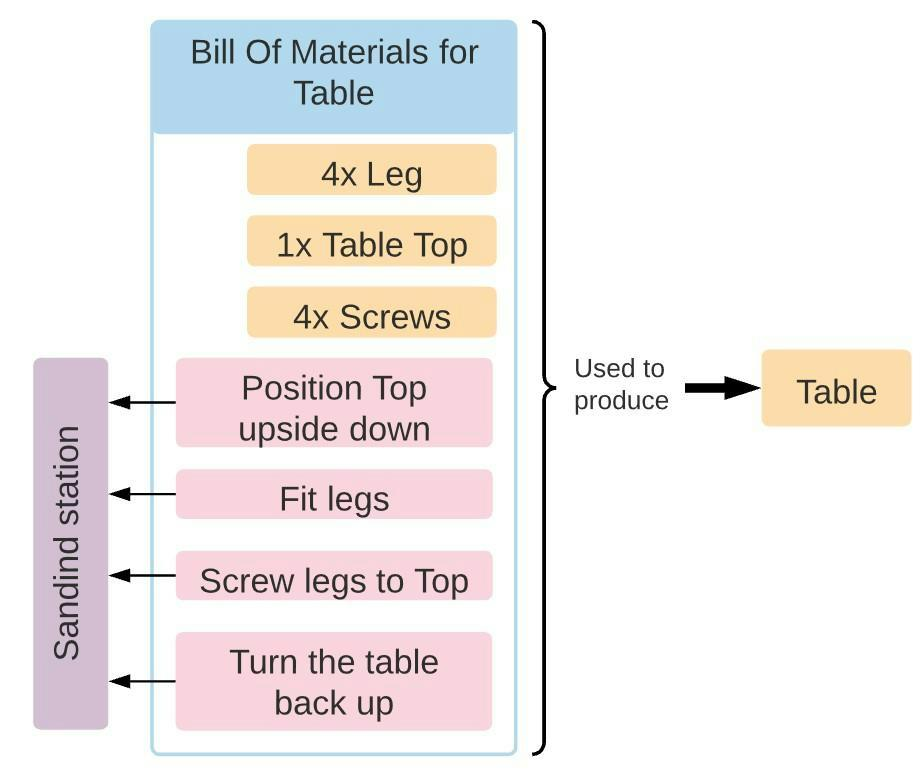
\includegraphics[width=441.8pt,height=372.32pt]{latexImage_bd93213ad077bb7e1ac2cb22b99270a9.png}}
\end{picture}
\newpage
\begin{tikzpicture}[overlay]\path(0pt,0pt);\end{tikzpicture}
\begin{picture}(-5,0)(2.5,0)
\put(500.14,-727.616){\fontsize{12}{1}\usefont{T1}{ptm}{m}{n}\selectfont\color{color_29791}33}
\put(512.14,-727.616){\fontsize{12}{1}\usefont{T1}{ptm}{m}{n}\selectfont\color{color_29791} }
\put(515.14,-727.616){\fontsize{12}{1}\usefont{T1}{ptm}{m}{n}\selectfont\color{color_29791} }
\put(70.104,-742.496){\fontsize{10.56}{1}\usefont{T1}{ptm}{m}{n}\selectfont\color{color_29791} }
\put(72.744,-742.496){\fontsize{12}{1}\usefont{T1}{ptm}{m}{n}\selectfont\color{color_29791} }
\put(515.74,-266.29){\fontsize{12}{1}\usefont{T1}{ptm}{m}{n}\selectfont\color{color_29791} }
\put(518.74,-266.29){\fontsize{12}{1}\usefont{T1}{ptm}{m}{n}\selectfont\color{color_29791} }
\put(248.81,-278.65){\fontsize{12}{1}\usefont{T1}{ptm}{m}{n}\selectfont\color{color_29791}圖}
\put(260.93,-278.65){\fontsize{12}{1}\usefont{T1}{ptm}{b}{n}\selectfont\color{color_29791}25}
\put(272.81,-278.65){\fontsize{12}{1}\usefont{T1}{ptm}{m}{n}\selectfont\color{color_29791}簡化訂}
\put(308.918,-278.65){\fontsize{12}{1}\usefont{T1}{ptm}{m}{n}\selectfont\color{color_29791}單圖}
\put(333.07,-278.65){\fontsize{12}{1}\usefont{T1}{ptm}{b}{n}\selectfont\color{color_29791} }
\put(335.95,-278.65){\fontsize{12}{1}\usefont{T1}{ptm}{m}{n}\selectfont\color{color_29791} }
\put(70.104,-296.05){\fontsize{12}{1}\usefont{T1}{ptm}{m}{n}\selectfont\color{color_29791} }
\put(73.104,-296.05){\fontsize{12}{1}\usefont{T1}{ptm}{m}{n}\selectfont\color{color_29791} }
\put(70.104,-310.93){\fontsize{12}{1}\usefont{T1}{ptm}{m}{n}\selectfont\color{color_29791} }
\put(73.104,-310.93){\fontsize{12}{1}\usefont{T1}{ptm}{m}{n}\selectfont\color{color_29791} }
\put(515.74,-530.07){\fontsize{12}{1}\usefont{T1}{ptm}{m}{n}\selectfont\color{color_29791} }
\put(518.74,-530.07){\fontsize{12}{1}\usefont{T1}{ptm}{m}{n}\selectfont\color{color_29791} }
\put(242.69,-550.71){\fontsize{12}{1}\usefont{T1}{ptm}{m}{n}\selectfont\color{color_29791}圖}
\put(254.81,-550.71){\fontsize{12}{1}\usefont{T1}{ptm}{b}{n}\selectfont\color{color_29791}26 }
\put(269.81,-550.71){\fontsize{12}{1}\usefont{T1}{ptm}{b}{n}\selectfont\color{color_29791}WO}
\put(291.05,-550.71){\fontsize{12}{1}\usefont{T1}{ptm}{m}{n}\selectfont\color{color_29791}操作介面}
\put(339.19,-550.71){\fontsize{12}{1}\usefont{T1}{ptm}{b}{n}\selectfont\color{color_29791} }
\put(342.07,-550.71){\fontsize{12}{1}\usefont{T1}{ptm}{m}{n}\selectfont\color{color_29791} }
\put(70.104,-567.99){\fontsize{12}{1}\usefont{T1}{ptm}{m}{n}\selectfont\color{color_29791} }
\put(73.104,-567.99){\fontsize{12}{1}\usefont{T1}{ptm}{m}{n}\selectfont\color{color_29791} }
\put(70.104,-582.99){\fontsize{12}{1}\usefont{T1}{ptm}{m}{n}\selectfont\color{color_29791} }
\put(73.104,-582.99){\fontsize{12}{1}\usefont{T1}{ptm}{m}{n}\selectfont\color{color_29791} }
\put(70.104,-619.5){\fontsize{11.04}{1}\usefont{T1}{ptm}{m}{n}\selectfont\color{color_29791} }
\put(124.1,-619.5){\fontsize{12}{1}\usefont{T1}{ptm}{b}{n}\selectfont\color{color_29791}5.1.3.5. }
\put(163.1,-619.5){\fontsize{12}{1}\usefont{T1}{ptm}{b}{n}\selectfont\color{color_29791} }
\put(224.81,-619.5){\fontsize{12}{1}\usefont{T1}{ptm}{m}{n}\selectfont\color{color_29791}工程變更}
\put(272.918,-619.5){\fontsize{12}{1}\usefont{T1}{ptm}{m}{n}\selectfont\color{color_29791}單}
\put(285.05,-619.5){\fontsize{12}{1}\usefont{T1}{ptm}{b}{n}\selectfont\color{color_29791}  }
\put(290.93,-619.5){\fontsize{12}{1}\usefont{T1}{ptm}{m}{n}\selectfont\color{color_29791} }
\put(82.944,-649.26){\fontsize{12}{1}\usefont{T1}{ptm}{m}{n}\selectfont\color{color_29791} }
\put(69.384,-665.1){\fontsize{12}{1}\usefont{T1}{ptm}{m}{n}\selectfont\color{color_29791}如第}
\put(93.38,-665.1){\fontsize{12}{1}\usefont{T1}{ptm}{m}{n}\selectfont\color{color_29791}2}
\put(99.38,-665.1){\fontsize{12}{1}\usefont{T1}{ptm}{m}{n}\selectfont\color{color_29791}章開頭所述}
\put(159.38,-665.1){\fontsize{12}{1}\usefont{T1}{ptm}{m}{n}\selectfont\color{color_29791},}
\put(171.38,-665.1){\fontsize{12}{1}\usefont{T1}{ptm}{m}{n}\selectfont\color{color_29791}Odoo}
\put(198.05,-665.1){\fontsize{12}{1}\usefont{T1}{ptm}{m}{n}\selectfont\color{color_29791}管理軟體主要將}
\put(282.05,-665.1){\fontsize{12}{1}\usefont{T1}{ptm}{m}{n}\selectfont\color{color_29791}P}
\put(288.878,-665.1){\fontsize{12}{1}\usefont{T1}{ptm}{m}{n}\selectfont\color{color_29791}L}
\put(295.958,-665.1){\fontsize{12}{1}\usefont{T1}{ptm}{m}{n}\selectfont\color{color_29791}M}
\put(306.77,-665.1){\fontsize{12}{1}\usefont{T1}{ptm}{m}{n}\selectfont\color{color_29791}視為跟蹤變更和改進的工具}
\put(450.82,-665.1){\fontsize{12}{1}\usefont{T1}{ptm}{m}{n}\selectfont\color{color_29791}。}
\put(462.82,-665.1){\fontsize{12}{1}\usefont{T1}{ptm}{m}{n}\selectfont\color{color_29791}它的應用}
\put(69.384,-682.856){\fontsize{12}{1}\usefont{T1}{ptm}{m}{n}\selectfont\color{color_29791}模組是正常製造流程的外部}
\put(213.41,-682.856){\fontsize{12}{1}\usefont{T1}{ptm}{m}{n}\selectfont\color{color_29791},}
\put(225.41,-682.856){\fontsize{12}{1}\usefont{T1}{ptm}{m}{n}\selectfont\color{color_29791}但充當其擴展}
\put(297.41,-682.856){\fontsize{12}{1}\usefont{T1}{ptm}{m}{n}\selectfont\color{color_29791}。}
\put(309.41,-682.856){\fontsize{12}{1}\usefont{T1}{ptm}{m}{n}\selectfont\color{color_29791}其重點專案類是工程變更單}
\put(453.46,-682.856){\fontsize{12}{1}\usefont{T1}{ptm}{m}{n}\selectfont\color{color_29791} }
\put(464.62,-682.856){\fontsize{12}{1}\usefont{T1}{ptm}{m}{n}\selectfont\color{color_29791}(}
\put(476.62,-682.856){\fontsize{12}{1}\usefont{T1}{ptm}{m}{n}\selectfont\color{color_29791}ECO}
\put(500.62,-682.856){\fontsize{12}{1}\usefont{T1}{ptm}{m}{n}\selectfont\color{color_29791})。}
\put(524.5,-682.856){\fontsize{12}{1}\usefont{T1}{ptm}{m}{n}\selectfont\color{color_29791}  }
\put(530.5,-682.856){\fontsize{12}{1}\usefont{T1}{ptm}{m}{n}\selectfont\color{color_29791} }
\put(84.264,-700.256){\fontsize{12}{1}\usefont{T1}{ptm}{m}{n}\selectfont\color{color_29791} }
\put(87.26,-700.256){\fontsize{12}{1}\usefont{T1}{ptm}{m}{n}\selectfont\color{color_29791} }
\put(73.75,-266.15){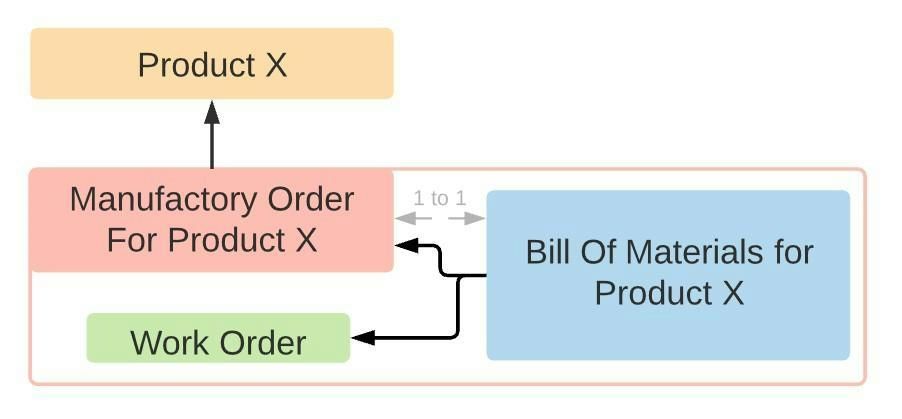
\includegraphics[width=441.9pt,height=205.25pt]{latexImage_aa75004b8d3b77865a714b77144a19d8.png}}
\put(73.75,-530.03){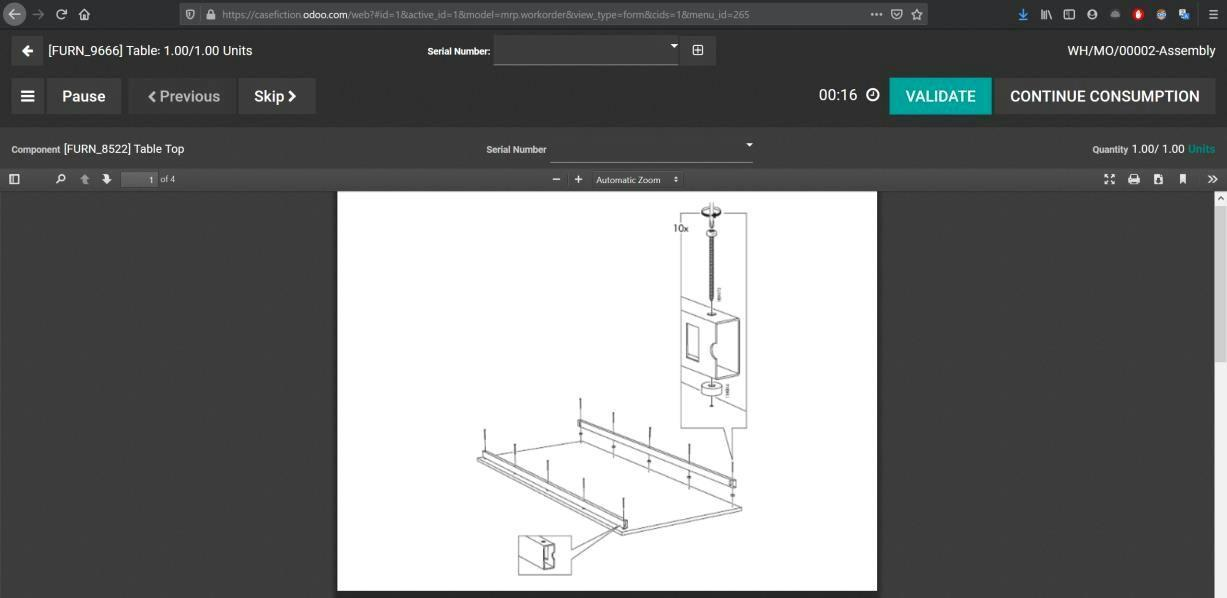
\includegraphics[width=441.9pt,height=215.45pt]{latexImage_4865ed325f1b5683d7fc6027983dfe91.png}}
\end{picture}
\newpage
\begin{tikzpicture}[overlay]\path(0pt,0pt);\end{tikzpicture}
\begin{picture}(-5,0)(2.5,0)
\put(500.14,-727.616){\fontsize{12}{1}\usefont{T1}{ptm}{m}{n}\selectfont\color{color_29791}34}
\put(512.14,-727.616){\fontsize{12}{1}\usefont{T1}{ptm}{m}{n}\selectfont\color{color_29791} }
\put(515.14,-727.616){\fontsize{12}{1}\usefont{T1}{ptm}{m}{n}\selectfont\color{color_29791} }
\put(70.104,-742.496){\fontsize{10.56}{1}\usefont{T1}{ptm}{m}{n}\selectfont\color{color_29791} }
\put(72.744,-742.496){\fontsize{12}{1}\usefont{T1}{ptm}{m}{n}\selectfont\color{color_29791} }
\put(82.944,-72.09998){\fontsize{12}{1}\usefont{T1}{ptm}{m}{n}\selectfont\color{color_29791}ECO }
\put(69.384,-87.94){\fontsize{12}{1}\usefont{T1}{ptm}{m}{n}\selectfont\color{color_29791}是一個專案類}
\put(141.38,-87.94){\fontsize{12}{1}\usefont{T1}{ptm}{m}{n}\selectfont\color{color_29791},}
\put(153.38,-87.94){\fontsize{12}{1}\usefont{T1}{ptm}{m}{n}\selectfont\color{color_29791}它概述了對產品或將受更改影響的部件的擬議更改}
\put(417.43,-87.94){\fontsize{12}{1}\usefont{T1}{ptm}{m}{n}\selectfont\color{color_29791}。}
\put(429.43,-87.94){\fontsize{12}{1}\usefont{T1}{ptm}{m}{n}\selectfont\color{color_29791}換句話說}
\put(477.46,-87.94){\fontsize{12}{1}\usefont{T1}{ptm}{m}{n}\selectfont\color{color_29791},}
\put(489.46,-87.94){\fontsize{12}{1}\usefont{T1}{ptm}{m}{n}\selectfont\color{color_29791}是}
\put(69.384,-105.7){\fontsize{12}{1}\usefont{T1}{ptm}{m}{n}\selectfont\color{color_29791}與給定產品相關的每個人的中央資訊中心}
\put(285.41,-105.7){\fontsize{12}{1}\usefont{T1}{ptm}{m}{n}\selectfont\color{color_29791}。}
\put(297.41,-105.7){\fontsize{12}{1}\usefont{T1}{ptm}{m}{n}\selectfont\color{color_29791}  }
\put(303.41,-105.7){\fontsize{12}{1}\usefont{T1}{ptm}{m}{n}\selectfont\color{color_29791} }
\put(84.264,-123.1){\fontsize{12}{1}\usefont{T1}{ptm}{m}{n}\selectfont\color{color_29791} }
\put(87.26,-123.1){\fontsize{12}{1}\usefont{T1}{ptm}{m}{n}\selectfont\color{color_29791} }
\put(82.944,-139.18){\fontsize{12}{1}\usefont{T1}{ptm}{m}{n}\selectfont\color{color_29791}這個想法是發出需要更改產品項或}
\put(262.97,-139.18){\fontsize{12}{1}\usefont{T1}{ptm}{m}{n}\selectfont\color{color_29791} }
\put(485.14,-139.18){\fontsize{12}{1}\usefont{T1}{ptm}{m}{n}\selectfont\color{color_29791}B}
\put(493.06,-139.18){\fontsize{12}{1}\usefont{T1}{ptm}{m}{n}\selectfont\color{color_29791}OM}
\put(512.488,-139.18){\fontsize{12}{1}\usefont{T1}{ptm}{m}{n}\selectfont\color{color_29791} }
\put(69.384,-156.82){\fontsize{12}{1}\usefont{T1}{ptm}{m}{n}\selectfont\color{color_29791}項的信號}
\put(117.38,-156.82){\fontsize{12}{1}\usefont{T1}{ptm}{m}{n}\selectfont\color{color_29791},}
\put(129.38,-156.82){\fontsize{12}{1}\usefont{T1}{ptm}{m}{n}\selectfont\color{color_29791}保留與更改相關的檔並應用更改}
\put(297.41,-156.82){\fontsize{12}{1}\usefont{T1}{ptm}{m}{n}\selectfont\color{color_29791},}
\put(309.41,-156.82){\fontsize{12}{1}\usefont{T1}{ptm}{m}{n}\selectfont\color{color_29791}或者至少發出已實施更改的信號}
\put(477.46,-156.82){\fontsize{12}{1}\usefont{T1}{ptm}{m}{n}\selectfont\color{color_29791},}
\put(489.46,-156.82){\fontsize{12}{1}\usefont{T1}{ptm}{m}{n}\selectfont\color{color_29791}同}
\put(69.384,-174.46){\fontsize{12}{1}\usefont{T1}{ptm}{m}{n}\selectfont\color{color_29791}時保留所有先前更改的歷史記錄}
\put(237.41,-174.46){\fontsize{12}{1}\usefont{T1}{ptm}{m}{n}\selectfont\color{color_29791}。}
\put(249.41,-174.46){\fontsize{12}{1}\usefont{T1}{ptm}{m}{n}\selectfont\color{color_29791}所有這些都在未來非常有用}
\put(393.43,-174.46){\fontsize{12}{1}\usefont{T1}{ptm}{m}{n}\selectfont\color{color_29791},}
\put(405.43,-174.46){\fontsize{12}{1}\usefont{T1}{ptm}{m}{n}\selectfont\color{color_29791}並作為簡化產品開}
\put(69.384,-192.22){\fontsize{12}{1}\usefont{T1}{ptm}{m}{n}\selectfont\color{color_29791}發和説明改進產品}
\put(165.38,-192.22){\fontsize{12}{1}\usefont{T1}{ptm}{m}{n}\selectfont\color{color_29791}/}
\put(168.74,-192.22){\fontsize{12}{1}\usefont{T1}{ptm}{m}{n}\selectfont\color{color_29791}生產的過程}
\put(228.77,-192.22){\fontsize{12}{1}\usefont{T1}{ptm}{m}{n}\selectfont\color{color_29791}。}
\put(240.77,-192.22){\fontsize{12}{1}\usefont{T1}{ptm}{m}{n}\selectfont\color{color_29791}  }
\put(246.77,-192.22){\fontsize{12}{1}\usefont{T1}{ptm}{m}{n}\selectfont\color{color_29791} }
\put(84.264,-209.62){\fontsize{12}{1}\usefont{T1}{ptm}{m}{n}\selectfont\color{color_29791} }
\put(87.26,-209.62){\fontsize{12}{1}\usefont{T1}{ptm}{m}{n}\selectfont\color{color_29791} }
\put(515.74,-451.47){\fontsize{12}{1}\usefont{T1}{ptm}{m}{n}\selectfont\color{color_29791} }
\put(518.74,-451.47){\fontsize{12}{1}\usefont{T1}{ptm}{m}{n}\selectfont\color{color_29791} }
\put(229.97,-472.11){\fontsize{12}{1}\usefont{T1}{ptm}{m}{n}\selectfont\color{color_29791}圖}
\put(242.09,-472.11){\fontsize{12}{1}\usefont{T1}{ptm}{b}{n}\selectfont\color{color_29791}27}
\put(253.97,-472.11){\fontsize{12}{1}\usefont{T1}{ptm}{m}{n}\selectfont\color{color_29791}簡化的}
\put(290.09,-472.11){\fontsize{12}{1}\usefont{T1}{ptm}{b}{n}\selectfont\color{color_29791}E}
\put(298.118,-472.11){\fontsize{12}{1}\usefont{T1}{ptm}{b}{n}\selectfont\color{color_29791}CO}
\put(316.03,-472.11){\fontsize{12}{1}\usefont{T1}{ptm}{m}{n}\selectfont\color{color_29791}功能圖}
\put(352.03,-472.11){\fontsize{12}{1}\usefont{T1}{ptm}{b}{n}\selectfont\color{color_29791} }
\put(355.03,-472.11){\fontsize{12}{1}\usefont{T1}{ptm}{m}{n}\selectfont\color{color_29791} }
\put(70.104,-489.39){\fontsize{12}{1}\usefont{T1}{ptm}{m}{n}\selectfont\color{color_29791} }
\put(73.104,-489.39){\fontsize{12}{1}\usefont{T1}{ptm}{m}{n}\selectfont\color{color_29791} }
\put(87.38,-506.55){\fontsize{14.04}{1}\usefont{T1}{ptm}{b}{n}\selectfont\color{color_29791}5}
\put(94.44212,-506.55){\fontsize{14.04}{1}\usefont{T1}{ptm}{b}{n}\selectfont\color{color_29791}.2. }
\put(111.86,-506.55){\fontsize{14.04}{1}\usefont{T1}{ptm}{m}{n}\selectfont\color{color_29791}開始模擬}
\put(168.14,-506.55){\fontsize{14.04}{1}\usefont{T1}{ptm}{b}{n}\selectfont\color{color_29791}  }
\put(174.98,-506.55){\fontsize{14.04}{1}\usefont{T1}{ptm}{b}{n}\selectfont\color{color_29791} }
\put(105.38,-552.51){\fontsize{12.96}{1}\usefont{T1}{ptm}{b}{n}\selectfont\color{color_29791}5.2.1. }
\put(137.78,-552.51){\fontsize{12.96}{1}\usefont{T1}{ptm}{m}{n}\selectfont\color{color_29791}為}
\put(150.8437,-552.51){\fontsize{12.96}{1}\usefont{T1}{ptm}{m}{n}\selectfont\color{color_29791}模}
\put(163.9073,-552.51){\fontsize{12.96}{1}\usefont{T1}{ptm}{m}{n}\selectfont\color{color_29791}擬}
\put(176.971,-552.51){\fontsize{12.96}{1}\usefont{T1}{ptm}{m}{n}\selectfont\color{color_29791}選擇}
\put(202.9947,-552.51){\fontsize{12.96}{1}\usefont{T1}{ptm}{m}{n}\selectfont\color{color_29791}的軟}
\put(229.0184,-552.51){\fontsize{12.96}{1}\usefont{T1}{ptm}{m}{n}\selectfont\color{color_29791}體選}
\put(255.0421,-552.51){\fontsize{12.96}{1}\usefont{T1}{ptm}{m}{n}\selectfont\color{color_29791}項}
\put(268.25,-552.51){\fontsize{12.96}{1}\usefont{T1}{ptm}{b}{n}\selectfont\color{color_29791} }
\put(271.37,-552.51){\fontsize{12.96}{1}\usefont{T1}{ptm}{b}{n}\selectfont\color{color_29791} }
\put(82.944,-581.55){\fontsize{12}{1}\usefont{T1}{ptm}{m}{n}\selectfont\color{color_29791}對於此類比}
\put(142.94,-581.55){\fontsize{12}{1}\usefont{T1}{ptm}{m}{n}\selectfont\color{color_29791},}
\put(154.94,-581.55){\fontsize{12}{1}\usefont{T1}{ptm}{m}{n}\selectfont\color{color_29791}已決定通過其基於}
\put(250.97,-581.55){\fontsize{12}{1}\usefont{T1}{ptm}{m}{n}\selectfont\color{color_29791}W}
\put(261.41,-581.55){\fontsize{12}{1}\usefont{T1}{ptm}{m}{n}\selectfont\color{color_29791}e}
\put(266.69,-581.55){\fontsize{12}{1}\usefont{T1}{ptm}{m}{n}\selectfont\color{color_29791}b}
\put(272.69,-581.55){\fontsize{12}{1}\usefont{T1}{ptm}{m}{n}\selectfont\color{color_29791}的在線服務對}
\put(344.71,-581.55){\fontsize{12}{1}\usefont{T1}{ptm}{m}{n}\selectfont\color{color_29791}Odoo}
\put(371.35,-581.55){\fontsize{12}{1}\usefont{T1}{ptm}{m}{n}\selectfont\color{color_29791}軟體進行最佳評估}
\put(467.38,-581.55){\fontsize{12}{1}\usefont{T1}{ptm}{m}{n}\selectfont\color{color_29791}。}
\put(479.38,-581.55){\fontsize{12}{1}\usefont{T1}{ptm}{m}{n}\selectfont\color{color_29791}選擇}
\put(69.384,-599.34){\fontsize{12}{1}\usefont{T1}{ptm}{m}{n}\selectfont\color{color_29791}不使用該軟體的社區版的原因如下}
\put(249.41,-599.34){\fontsize{12}{1}\usefont{T1}{ptm}{m}{n}\selectfont\color{color_29791}:}
\put(261.41,-599.34){\fontsize{12}{1}\usefont{T1}{ptm}{m}{n}\selectfont\color{color_29791} }
\put(264.41,-599.34){\fontsize{12}{1}\usefont{T1}{ptm}{m}{n}\selectfont\color{color_29791} }
\put(84.264,-616.74){\fontsize{12}{1}\usefont{T1}{ptm}{m}{n}\selectfont\color{color_29791} }
\put(87.26,-616.74){\fontsize{12}{1}\usefont{T1}{ptm}{m}{n}\selectfont\color{color_29791} }
\put(102.26,-633.66){\fontsize{12}{1}\usefont{T1}{ptm}{m}{n}\selectfont\color{color_29791}}
\put(112.94,-633.66){\fontsize{12}{1}\usefont{T1}{uarial}{m}{n}\selectfont\color{color_29791} }
\put(120.26,-633.66){\fontsize{12}{1}\usefont{T1}{ptm}{m}{n}\selectfont\color{color_29791}使用基於}
\put(168.26,-633.66){\fontsize{12}{1}\usefont{T1}{ptm}{m}{n}\selectfont\color{color_29791} }
\put(490.9,-633.66){\fontsize{12}{1}\usefont{T1}{ptm}{m}{n}\selectfont\color{color_29791}W}
\put(501.34,-633.66){\fontsize{12}{1}\usefont{T1}{ptm}{m}{n}\selectfont\color{color_29791}e}
\put(506.62,-633.66){\fontsize{12}{1}\usefont{T1}{ptm}{m}{n}\selectfont\color{color_29791}b}
\put(512.5,-633.66){\fontsize{12}{1}\usefont{T1}{ptm}{m}{n}\selectfont\color{color_29791} }
\put(120.26,-651.3){\fontsize{12}{1}\usefont{T1}{ptm}{m}{n}\selectfont\color{color_29791}的服務作為本地或遠端管理伺服器的實用性}
\put(348.31,-651.3){\fontsize{12}{1}\usefont{T1}{ptm}{m}{n}\selectfont\color{color_29791}。}
\put(360.31,-651.3){\fontsize{12}{1}\usefont{T1}{ptm}{m}{n}\selectfont\color{color_29791}儘管社區應用程式作為這項}
\put(120.26,-668.94){\fontsize{12}{1}\usefont{T1}{ptm}{m}{n}\selectfont\color{color_29791}工作研究的一部分進行了測試}
\put(276.29,-668.94){\fontsize{12}{1}\usefont{T1}{ptm}{m}{n}\selectfont\color{color_29791},}
\put(288.29,-668.94){\fontsize{12}{1}\usefont{T1}{ptm}{m}{n}\selectfont\color{color_29791}並且被認為是一個非常初學者友好的伺服}
\put(120.26,-686.576){\fontsize{12}{1}\usefont{T1}{ptm}{m}{n}\selectfont\color{color_29791}器應用程式}
\put(181.49,-686.576){\fontsize{12}{1}\usefont{T1}{ptm}{m}{n}\selectfont\color{color_29791},}
\put(193.73,-686.576){\fontsize{12}{1}\usefont{T1}{ptm}{m}{n}\selectfont\color{color_29791}但事實是}
\put(242.69,-686.576){\fontsize{12}{1}\usefont{T1}{ptm}{m}{n}\selectfont\color{color_29791},}
\put(254.93,-686.576){\fontsize{12}{1}\usefont{T1}{ptm}{m}{n}\selectfont\color{color_29791}託管伺服器本身就是一項需要經驗和知識的工作}
\put(512.14,-686.576){\fontsize{12}{1}\usefont{T1}{ptm}{m}{n}\selectfont\color{color_29791}。}
\put(524.5,-686.576){\fontsize{12}{1}\usefont{T1}{ptm}{m}{n}\selectfont\color{color_29791} }
\put(120.26,-704.096){\fontsize{12}{1}\usefont{T1}{ptm}{m}{n}\selectfont\color{color_29791}關於這種應用}
\put(192.29,-704.096){\fontsize{12}{1}\usefont{T1}{ptm}{m}{n}\selectfont\color{color_29791},}
\put(204.29,-704.096){\fontsize{12}{1}\usefont{T1}{ptm}{m}{n}\selectfont\color{color_29791}市場已經轉向產品即服務}
\put(336.31,-704.096){\fontsize{12}{1}\usefont{T1}{ptm}{m}{n}\selectfont\color{color_29791},}
\put(348.31,-704.096){\fontsize{12}{1}\usefont{T1}{ptm}{m}{n}\selectfont\color{color_29791}這是有充分理由的}
\put(444.31,-704.096){\fontsize{12}{1}\usefont{T1}{ptm}{m}{n}\selectfont\color{color_29791}。}
\put(456.34,-704.096){\fontsize{12}{1}\usefont{T1}{ptm}{m}{n}\selectfont\color{color_29791}在撰寫本}
\put(73.75,-451.42){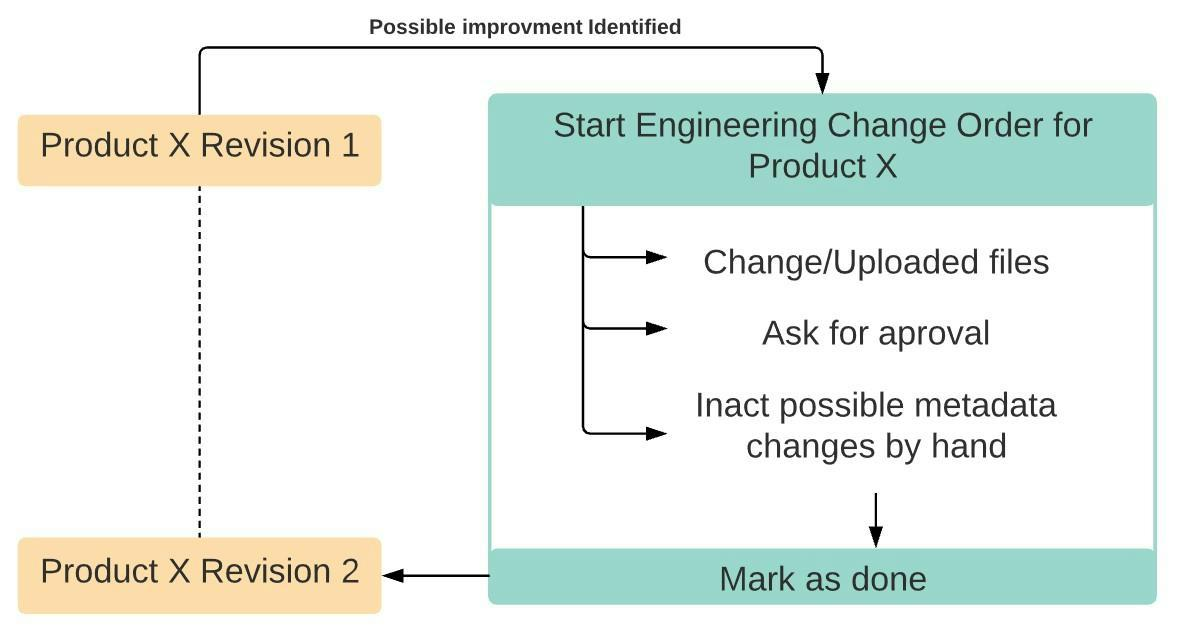
\includegraphics[width=441.9pt,height=238.05pt]{latexImage_3aae4d135289b2440dacb3b97c2f4364.png}}
\end{picture}
\newpage
\begin{tikzpicture}[overlay]\path(0pt,0pt);\end{tikzpicture}
\begin{picture}(-5,0)(2.5,0)
\put(500.14,-727.616){\fontsize{12}{1}\usefont{T1}{ptm}{m}{n}\selectfont\color{color_29791}35}
\put(512.14,-727.616){\fontsize{12}{1}\usefont{T1}{ptm}{m}{n}\selectfont\color{color_29791} }
\put(515.14,-727.616){\fontsize{12}{1}\usefont{T1}{ptm}{m}{n}\selectfont\color{color_29791} }
\put(70.104,-742.496){\fontsize{10.56}{1}\usefont{T1}{ptm}{m}{n}\selectfont\color{color_29791} }
\put(72.744,-742.496){\fontsize{12}{1}\usefont{T1}{ptm}{m}{n}\selectfont\color{color_29791} }
\put(120.26,-72.34003){\fontsize{12}{1}\usefont{T1}{ptm}{m}{n}\selectfont\color{color_29791}文時}
\put(144.26,-72.34003){\fontsize{12}{1}\usefont{T1}{ptm}{m}{n}\selectfont\color{color_29791},}
\put(156.26,-72.34003){\fontsize{12}{1}\usefont{T1}{ptm}{m}{n}\selectfont\color{color_29791}C}
\put(164.288,-72.34003){\fontsize{12}{1}\usefont{T1}{ptm}{m}{n}\selectfont\color{color_29791}OV}
\put(181.676,-72.34003){\fontsize{12}{1}\usefont{T1}{ptm}{m}{n}\selectfont\color{color_29791}I}
\put(185.516,-72.34003){\fontsize{12}{1}\usefont{T1}{ptm}{m}{n}\selectfont\color{color_29791}D}
\put(194.21,-72.34003){\fontsize{12}{1}\usefont{T1}{ptm}{m}{n}\selectfont\color{color_29791}-}
\put(198.17,-72.34003){\fontsize{12}{1}\usefont{T1}{ptm}{m}{n}\selectfont\color{color_29791}19 }
\put(235.85,-72.34003){\fontsize{12}{1}\usefont{T1}{ptm}{m}{n}\selectfont\color{color_29791}大流行迫使許多員工遠端工作}
\put(391.87,-72.34003){\fontsize{12}{1}\usefont{T1}{ptm}{m}{n}\selectfont\color{color_29791},}
\put(403.87,-72.34003){\fontsize{12}{1}\usefont{T1}{ptm}{m}{n}\selectfont\color{color_29791}並向市場表明}
\put(475.9,-72.34003){\fontsize{12}{1}\usefont{T1}{ptm}{m}{n}\selectfont\color{color_29791} }
\put(501.58,-72.34003){\fontsize{12}{1}\usefont{T1}{ptm}{m}{n}\selectfont\color{color_29791}I}
\put(505.42,-72.34003){\fontsize{12}{1}\usefont{T1}{ptm}{m}{n}\selectfont\color{color_29791}T}
\put(512.5001,-72.34003){\fontsize{12}{1}\usefont{T1}{ptm}{m}{n}\selectfont\color{color_29791} }
\put(120.26,-90.09998){\fontsize{12}{1}\usefont{T1}{ptm}{m}{n}\selectfont\color{color_29791}不是一項簡單的工作}
\put(228.29,-90.09998){\fontsize{12}{1}\usefont{T1}{ptm}{m}{n}\selectfont\color{color_29791},}
\put(240.29,-90.09998){\fontsize{12}{1}\usefont{T1}{ptm}{m}{n}\selectfont\color{color_29791}W}
\put(250.73,-90.09998){\fontsize{12}{1}\usefont{T1}{ptm}{m}{n}\selectfont\color{color_29791}e}
\put(256.01,-90.09998){\fontsize{12}{1}\usefont{T1}{ptm}{m}{n}\selectfont\color{color_29791}b }
\put(265.01,-90.09998){\fontsize{12}{1}\usefont{T1}{ptm}{m}{n}\selectfont\color{color_29791}服務是一個有吸引力的選擇}
\put(409.03,-90.09998){\fontsize{12}{1}\usefont{T1}{ptm}{m}{n}\selectfont\color{color_29791}。}
\put(421.03,-90.09998){\fontsize{12}{1}\usefont{T1}{ptm}{m}{n}\selectfont\color{color_29791}  }
\put(427.03,-90.09998){\fontsize{12}{1}\usefont{T1}{ptm}{m}{n}\selectfont\color{color_29791} }
\put(84.264,-107.5){\fontsize{12}{1}\usefont{T1}{ptm}{m}{n}\selectfont\color{color_29791} }
\put(87.26,-107.5){\fontsize{12}{1}\usefont{T1}{ptm}{m}{n}\selectfont\color{color_29791} }
\put(102.26,-124.54){\fontsize{12}{1}\usefont{T1}{ptm}{m}{n}\selectfont\color{color_29791}}
\put(112.94,-124.54){\fontsize{12}{1}\usefont{T1}{uarial}{m}{n}\selectfont\color{color_29791} }
\put(120.26,-124.54){\fontsize{12}{1}\usefont{T1}{ptm}{m}{n}\selectfont\color{color_29791}缺少}
\put(144.26,-124.54){\fontsize{12}{1}\usefont{T1}{ptm}{m}{n}\selectfont\color{color_29791}Odoo}
\put(170.9,-124.54){\fontsize{12}{1}\usefont{T1}{ptm}{m}{n}\selectfont\color{color_29791}社區版的官方}
\put(242.93,-124.54){\fontsize{12}{1}\usefont{T1}{ptm}{m}{n}\selectfont\color{color_29791}OdooP}
\put(276.398,-124.54){\fontsize{12}{1}\usefont{T1}{ptm}{m}{n}\selectfont\color{color_29791}L}
\put(283.478,-124.54){\fontsize{12}{1}\usefont{T1}{ptm}{m}{n}\selectfont\color{color_29791}M}
\put(294.17,-124.54){\fontsize{12}{1}\usefont{T1}{ptm}{m}{n}\selectfont\color{color_29791}應用程式}
\put(342.19,-124.54){\fontsize{12}{1}\usefont{T1}{ptm}{m}{n}\selectfont\color{color_29791}。}
\put(354.31,-124.54){\fontsize{12}{1}\usefont{T1}{ptm}{m}{n}\selectfont\color{color_29791}儘管}
\put(378.31,-124.54){\fontsize{12}{1}\usefont{T1}{ptm}{m}{n}\selectfont\color{color_29791}Odoo}
\put(404.95,-124.54){\fontsize{12}{1}\usefont{T1}{ptm}{m}{n}\selectfont\color{color_29791}的社區版有大量的}
\put(120.26,-142.18){\fontsize{12}{1}\usefont{T1}{ptm}{m}{n}\selectfont\color{color_29791}社區應用程式}
\put(192.29,-142.18){\fontsize{12}{1}\usefont{T1}{ptm}{m}{n}\selectfont\color{color_29791},}
\put(204.29,-142.18){\fontsize{12}{1}\usefont{T1}{ptm}{m}{n}\selectfont\color{color_29791}但這些應用程式的組織}
\put(324.31,-142.18){\fontsize{12}{1}\usefont{T1}{ptm}{m}{n}\selectfont\color{color_29791}、}
\put(336.31,-142.18){\fontsize{12}{1}\usefont{T1}{ptm}{m}{n}\selectfont\color{color_29791}描述}
\put(360.31,-142.18){\fontsize{12}{1}\usefont{T1}{ptm}{m}{n}\selectfont\color{color_29791}、}
\put(372.31,-142.18){\fontsize{12}{1}\usefont{T1}{ptm}{m}{n}\selectfont\color{color_29791}集成和支援充其量只能被}
\put(120.26,-159.82){\fontsize{12}{1}\usefont{T1}{ptm}{m}{n}\selectfont\color{color_29791}發現}
\put(144.26,-159.82){\fontsize{12}{1}\usefont{T1}{ptm}{m}{n}\selectfont\color{color_29791}。}
\put(156.26,-159.82){\fontsize{12}{1}\usefont{T1}{ptm}{m}{n}\selectfont\color{color_29791}與其依賴可能跟不上主要軟體的應用程式}
\put(372.31,-159.82){\fontsize{12}{1}\usefont{T1}{ptm}{m}{n}\selectfont\color{color_29791},}
\put(384.31,-159.82){\fontsize{12}{1}\usefont{T1}{ptm}{m}{n}\selectfont\color{color_29791}不如決定如果基於官方}
\put(120.26,-177.34){\fontsize{12}{1}\usefont{T1}{ptm}{m}{n}\selectfont\color{color_29791}應用程式}
\put(168.26,-177.34){\fontsize{12}{1}\usefont{T1}{ptm}{m}{n}\selectfont\color{color_29791},}
\put(180.29,-177.34){\fontsize{12}{1}\usefont{T1}{ptm}{m}{n}\selectfont\color{color_29791}對平臺評估會更公平}
\put(288.29,-177.34){\fontsize{12}{1}\usefont{T1}{ptm}{m}{n}\selectfont\color{color_29791}。}
\put(300.29,-177.34){\fontsize{12}{1}\usefont{T1}{ptm}{m}{n}\selectfont\color{color_29791}也就是說}
\put(348.31,-177.34){\fontsize{12}{1}\usefont{T1}{ptm}{m}{n}\selectfont\color{color_29791},}
\put(360.31,-177.34){\fontsize{12}{1}\usefont{T1}{ptm}{m}{n}\selectfont\color{color_29791}僅僅依靠運氣來決定未來如}
\put(120.26,-194.98){\fontsize{12}{1}\usefont{T1}{ptm}{m}{n}\selectfont\color{color_29791}何支援它}
\put(168.26,-194.98){\fontsize{12}{1}\usefont{T1}{ptm}{m}{n}\selectfont\color{color_29791},}
\put(180.29,-194.98){\fontsize{12}{1}\usefont{T1}{ptm}{m}{n}\selectfont\color{color_29791}就拼湊出一個免費的解決方案是非常徒勞的}
\put(408.31,-194.98){\fontsize{12}{1}\usefont{T1}{ptm}{m}{n}\selectfont\color{color_29791}。}
\put(420.31,-194.98){\fontsize{12}{1}\usefont{T1}{ptm}{m}{n}\selectfont\color{color_29791}P}
\put(427.138,-194.98){\fontsize{12}{1}\usefont{T1}{ptm}{m}{n}\selectfont\color{color_29791}L}
\put(434.218,-194.98){\fontsize{12}{1}\usefont{T1}{ptm}{m}{n}\selectfont\color{color_29791}M }
\put(120.26,-212.74){\fontsize{12}{1}\usefont{T1}{ptm}{m}{n}\selectfont\color{color_29791}是這裡的重點}
\put(192.29,-212.74){\fontsize{12}{1}\usefont{T1}{ptm}{m}{n}\selectfont\color{color_29791},}
\put(204.29,-212.74){\fontsize{12}{1}\usefont{T1}{ptm}{m}{n}\selectfont\color{color_29791}所以這是一個不容置疑的情況}
\put(360.31,-212.74){\fontsize{12}{1}\usefont{T1}{ptm}{m}{n}\selectfont\color{color_29791}。}
\put(372.31,-212.74){\fontsize{12}{1}\usefont{T1}{ptm}{m}{n}\selectfont\color{color_29791}  }
\put(378.31,-212.74){\fontsize{12}{1}\usefont{T1}{ptm}{m}{n}\selectfont\color{color_29791} }
\put(84.264,-230.26){\fontsize{12}{1}\usefont{T1}{ptm}{m}{n}\selectfont\color{color_29791} }
\put(87.26,-230.26){\fontsize{12}{1}\usefont{T1}{ptm}{m}{n}\selectfont\color{color_29791} }
\put(82.944,-246.13){\fontsize{12}{1}\usefont{T1}{ptm}{m}{n}\selectfont\color{color_29791}在撰寫本文時}
\put(154.94,-246.13){\fontsize{12}{1}\usefont{T1}{ptm}{m}{n}\selectfont\color{color_29791},}
\put(166.94,-246.13){\fontsize{12}{1}\usefont{T1}{ptm}{m}{n}\selectfont\color{color_29791}Odoo}
\put(193.61,-246.13){\fontsize{12}{1}\usefont{T1}{ptm}{m}{n}\selectfont\color{color_29791}允許您選擇其額外功能之一}
\put(337.63,-246.13){\fontsize{12}{1}\usefont{T1}{ptm}{m}{n}\selectfont\color{color_29791},}
\put(349.63,-246.13){\fontsize{12}{1}\usefont{T1}{ptm}{m}{n}\selectfont\color{color_29791}例如}
\put(373.63,-246.13){\fontsize{12}{1}\usefont{T1}{ptm}{m}{n}\selectfont\color{color_29791}P}
\put(380.458,-246.13){\fontsize{12}{1}\usefont{T1}{ptm}{m}{n}\selectfont\color{color_29791}L}
\put(387.538,-246.13){\fontsize{12}{1}\usefont{T1}{ptm}{m}{n}\selectfont\color{color_29791}M}
\put(398.23,-246.13){\fontsize{12}{1}\usefont{T1}{ptm}{m}{n}\selectfont\color{color_29791},}
\put(410.23,-246.13){\fontsize{12}{1}\usefont{T1}{ptm}{m}{n}\selectfont\color{color_29791}並在其}
\put(446.338,-246.13){\fontsize{12}{1}\usefont{T1}{ptm}{m}{n}\selectfont\color{color_29791}雲託管伺服}
\put(69.384,-263.77){\fontsize{12}{1}\usefont{T1}{ptm}{m}{n}\selectfont\color{color_29791}器上無限期免費使用它}
\put(189.41,-263.77){\fontsize{12}{1}\usefont{T1}{ptm}{m}{n}\selectfont\color{color_29791}。}
\put(201.41,-263.77){\fontsize{12}{1}\usefont{T1}{ptm}{m}{n}\selectfont\color{color_29791}如果這項工作的唯一重點是}
\put(345.43,-263.77){\fontsize{12}{1}\usefont{T1}{ptm}{m}{n}\selectfont\color{color_29791} }
\put(487.9,-263.77){\fontsize{12}{1}\usefont{T1}{ptm}{m}{n}\selectfont\color{color_29791}P}
\put(494.728,-263.77){\fontsize{12}{1}\usefont{T1}{ptm}{m}{n}\selectfont\color{color_29791}L}
\put(501.808,-263.77){\fontsize{12}{1}\usefont{T1}{ptm}{m}{n}\selectfont\color{color_29791}M }
\put(69.384,-281.41){\fontsize{12}{1}\usefont{T1}{ptm}{m}{n}\selectfont\color{color_29791}和}
\put(81.384,-281.41){\fontsize{12}{1}\usefont{T1}{ptm}{m}{n}\selectfont\color{color_29791}製造}
\put(105.38,-281.41){\fontsize{12}{1}\usefont{T1}{ptm}{m}{n}\selectfont\color{color_29791},}
\put(117.38,-281.41){\fontsize{12}{1}\usefont{T1}{ptm}{m}{n}\selectfont\color{color_29791}這是一個非常有吸引力的選擇}
\put(273.41,-281.41){\fontsize{12}{1}\usefont{T1}{ptm}{m}{n}\selectfont\color{color_29791}。}
\put(285.41,-281.41){\fontsize{12}{1}\usefont{T1}{ptm}{m}{n}\selectfont\color{color_29791}然而}
\put(309.41,-281.41){\fontsize{12}{1}\usefont{T1}{ptm}{m}{n}\selectfont\color{color_29791},}
\put(321.43,-281.41){\fontsize{12}{1}\usefont{T1}{ptm}{m}{n}\selectfont\color{color_29791}這項工作的}
\put(381.43,-281.41){\fontsize{12}{1}\usefont{T1}{ptm}{m}{n}\selectfont\color{color_29791}MES}
\put(406.15,-281.41){\fontsize{12}{1}\usefont{T1}{ptm}{m}{n}\selectfont\color{color_29791}方面高度依賴於}
\put(490.18,-281.41){\fontsize{12}{1}\usefont{T1}{ptm}{m}{n}\selectfont\color{color_29791}Odo}
\put(69.384,-299.05){\fontsize{12}{1}\usefont{T1}{ptm}{m}{n}\selectfont\color{color_29791}o}
\put(75.384,-299.05){\fontsize{12}{1}\usefont{T1}{ptm}{m}{n}\selectfont\color{color_29791}的其他應用}
\put(135.38,-299.05){\fontsize{12}{1}\usefont{T1}{ptm}{m}{n}\selectfont\color{color_29791},}
\put(147.38,-299.05){\fontsize{12}{1}\usefont{T1}{ptm}{m}{n}\selectfont\color{color_29791}這意味著可以做的很少}
\put(267.41,-299.05){\fontsize{12}{1}\usefont{T1}{ptm}{m}{n}\selectfont\color{color_29791}。}
\put(279.41,-299.05){\fontsize{12}{1}\usefont{T1}{ptm}{m}{n}\selectfont\color{color_29791}為此}
\put(303.41,-299.05){\fontsize{12}{1}\usefont{T1}{ptm}{m}{n}\selectfont\color{color_29791},}
\put(315.43,-299.05){\fontsize{12}{1}\usefont{T1}{ptm}{m}{n}\selectfont\color{color_29791}實驗是在}
\put(363.43,-299.05){\fontsize{12}{1}\usefont{T1}{ptm}{m}{n}\selectfont\color{color_29791}Odoo}
\put(390.07,-299.05){\fontsize{12}{1}\usefont{T1}{ptm}{m}{n}\selectfont\color{color_29791}企業版的試用版中進行}
\put(69.384,-316.69){\fontsize{12}{1}\usefont{T1}{ptm}{m}{n}\selectfont\color{color_29791}的}
\put(81.384,-316.69){\fontsize{12}{1}\usefont{T1}{ptm}{m}{n}\selectfont\color{color_29791},}
\put(93.38,-316.69){\fontsize{12}{1}\usefont{T1}{ptm}{m}{n}\selectfont\color{color_29791}它允許使用者在}
\put(177.38,-316.69){\fontsize{12}{1}\usefont{T1}{ptm}{m}{n}\selectfont\color{color_29791}14}
\put(189.41,-316.69){\fontsize{12}{1}\usefont{T1}{ptm}{m}{n}\selectfont\color{color_29791}天內使用系統}
\put(261.41,-316.69){\fontsize{12}{1}\usefont{T1}{ptm}{m}{n}\selectfont\color{color_29791},}
\put(273.41,-316.69){\fontsize{12}{1}\usefont{T1}{ptm}{m}{n}\selectfont\color{color_29791}而沒有存儲或應用程式限制}
\put(417.43,-316.69){\fontsize{12}{1}\usefont{T1}{ptm}{m}{n}\selectfont\color{color_29791},}
\put(429.43,-316.69){\fontsize{12}{1}\usefont{T1}{ptm}{m}{n}\selectfont\color{color_29791}全部託管在}
\put(489.46,-316.69){\fontsize{12}{1}\usefont{T1}{ptm}{m}{n}\selectfont\color{color_29791}Odo}
\put(69.384,-334.45){\fontsize{12}{1}\usefont{T1}{ptm}{m}{n}\selectfont\color{color_29791}o}
\put(75.384,-334.45){\fontsize{12}{1}\usefont{T1}{ptm}{m}{n}\selectfont\color{color_29791}雲伺服器中}
\put(135.38,-334.45){\fontsize{12}{1}\usefont{T1}{ptm}{m}{n}\selectfont\color{color_29791}(}
\put(147.38,-334.45){\fontsize{12}{1}\usefont{T1}{ptm}{m}{n}\selectfont\color{color_29791}圖}
\put(159.38,-334.45){\fontsize{12}{1}\usefont{T1}{ptm}{m}{n}\selectfont\color{color_29791}17}
\put(171.38,-334.45){\fontsize{12}{1}\usefont{T1}{ptm}{m}{n}\selectfont\color{color_29791})。}
\put(195.41,-334.45){\fontsize{12}{1}\usefont{T1}{ptm}{m}{n}\selectfont\color{color_29791} }
\put(198.41,-334.45){\fontsize{12}{1}\usefont{T1}{ptm}{m}{n}\selectfont\color{color_29791} }
\put(70.104,-351.85){\fontsize{12}{1}\usefont{T1}{ptm}{m}{n}\selectfont\color{color_29791} }
\put(73.104,-351.85){\fontsize{12}{1}\usefont{T1}{ptm}{m}{n}\selectfont\color{color_29791} }
\put(105.38,-368.05){\fontsize{12.96}{1}\usefont{T1}{ptm}{b}{n}\selectfont\color{color_29791}5.2.2. }
\put(137.78,-368.05){\fontsize{12.96}{1}\usefont{T1}{ptm}{m}{n}\selectfont\color{color_29791}相}
\put(150.8437,-368.05){\fontsize{12.96}{1}\usefont{T1}{ptm}{m}{n}\selectfont\color{color_29791}關}
\put(163.9073,-368.05){\fontsize{12.96}{1}\usefont{T1}{ptm}{m}{n}\selectfont\color{color_29791}的}
\put(176.971,-368.05){\fontsize{12.96}{1}\usefont{T1}{ptm}{m}{n}\selectfont\color{color_29791}設置}
\put(202.9947,-368.05){\fontsize{12.96}{1}\usefont{T1}{ptm}{m}{n}\selectfont\color{color_29791}細節}
\put(229.13,-368.05){\fontsize{12.96}{1}\usefont{T1}{ptm}{b}{n}\selectfont\color{color_29791}  }
\put(235.61,-368.05){\fontsize{12.96}{1}\usefont{T1}{ptm}{b}{n}\selectfont\color{color_29791} }
\put(82.944,-396.97){\fontsize{12}{1}\usefont{T1}{ptm}{m}{n}\selectfont\color{color_29791}有關}
\put(106.94,-396.97){\fontsize{12}{1}\usefont{T1}{ptm}{m}{n}\selectfont\color{color_29791}Odoo}
\put(133.58,-396.97){\fontsize{12}{1}\usefont{T1}{ptm}{m}{n}\selectfont\color{color_29791}設置的一些細節與其製造功能的正常功能有關}
\put(373.63,-396.97){\fontsize{12}{1}\usefont{T1}{ptm}{m}{n}\selectfont\color{color_29791}。}
\put(385.63,-396.97){\fontsize{12}{1}\usefont{T1}{ptm}{m}{n}\selectfont\color{color_29791}也就是說}
\put(433.63,-396.97){\fontsize{12}{1}\usefont{T1}{ptm}{m}{n}\selectfont\color{color_29791},}
\put(445.66,-396.97){\fontsize{12}{1}\usefont{T1}{ptm}{m}{n}\selectfont\color{color_29791}在製造設置}
\put(69.384,-414.73){\fontsize{12}{1}\usefont{T1}{ptm}{m}{n}\selectfont\color{color_29791}中啟用工作訂單是正確使用工作訂單項}
\put(273.41,-414.73){\fontsize{12}{1}\usefont{T1}{ptm}{m}{n}\selectfont\color{color_29791}、}
\put(285.41,-414.73){\fontsize{12}{1}\usefont{T1}{ptm}{m}{n}\selectfont\color{color_29791}工作中心項和工序項的必要步驟}
\put(453.46,-414.73){\fontsize{12}{1}\usefont{T1}{ptm}{m}{n}\selectfont\color{color_29791}。}
\put(465.46,-414.73){\fontsize{12}{1}\usefont{T1}{ptm}{m}{n}\selectfont\color{color_29791}  }
\put(471.46,-414.73){\fontsize{12}{1}\usefont{T1}{ptm}{m}{n}\selectfont\color{color_29791} }
\put(84.264,-432.15){\fontsize{12}{1}\usefont{T1}{ptm}{m}{n}\selectfont\color{color_29791} }
\put(87.26,-432.15){\fontsize{12}{1}\usefont{T1}{ptm}{m}{n}\selectfont\color{color_29791} }
\put(82.944,-448.11){\fontsize{12}{1}\usefont{T1}{ptm}{m}{n}\selectfont\color{color_29791}為這項工作所做的一個假設是}
\put(238.97,-448.11){\fontsize{12}{1}\usefont{T1}{ptm}{m}{n}\selectfont\color{color_29791},}
\put(250.97,-448.11){\fontsize{12}{1}\usefont{T1}{ptm}{m}{n}\selectfont\color{color_29791}這是軟體}
\put(298.97,-448.11){\fontsize{12}{1}\usefont{T1}{ptm}{m}{n}\selectfont\color{color_29791}ERP}
\put(320.95,-448.11){\fontsize{12}{1}\usefont{T1}{ptm}{m}{n}\selectfont\color{color_29791}起源的保留}
\put(380.95,-448.11){\fontsize{12}{1}\usefont{T1}{ptm}{m}{n}\selectfont\color{color_29791},}
\put(392.95,-448.11){\fontsize{12}{1}\usefont{T1}{ptm}{m}{n}\selectfont\color{color_29791}因為如果您要使用}
\put(488.98,-448.11){\fontsize{12}{1}\usefont{T1}{ptm}{m}{n}\selectfont\color{color_29791}Odo}
\put(69.384,-465.75){\fontsize{12}{1}\usefont{T1}{ptm}{m}{n}\selectfont\color{color_29791}o}
\put(75.384,-465.75){\fontsize{12}{1}\usefont{T1}{ptm}{m}{n}\selectfont\color{color_29791}對製造進行任何嚴格的控制}
\put(219.41,-465.75){\fontsize{12}{1}\usefont{T1}{ptm}{m}{n}\selectfont\color{color_29791},}
\put(231.41,-465.75){\fontsize{12}{1}\usefont{T1}{ptm}{m}{n}\selectfont\color{color_29791}那麼默認情況下不啟用此設置是相當不直觀的}
\put(471.46,-465.75){\fontsize{12}{1}\usefont{T1}{ptm}{m}{n}\selectfont\color{color_29791}。}
\put(483.46,-465.75){\fontsize{12}{1}\usefont{T1}{ptm}{m}{n}\selectfont\color{color_29791}從}
\put(495.46,-465.75){\fontsize{12}{1}\usefont{T1}{ptm}{m}{n}\selectfont\color{color_29791} }
\put(69.384,-483.39){\fontsize{12}{1}\usefont{T1}{ptm}{m}{n}\selectfont\color{color_29791}Odoo }
\put(99.372,-483.39){\fontsize{12}{1}\usefont{T1}{ptm}{m}{n}\selectfont\color{color_29791}e}
\put(104.652,-483.39){\fontsize{12}{1}\usefont{T1}{ptm}{m}{n}\selectfont\color{color_29791}nter}
\put(123.252,-483.39){\fontsize{12}{1}\usefont{T1}{ptm}{m}{n}\selectfont\color{color_29791}p}
\put(129.36,-483.39){\fontsize{12}{1}\usefont{T1}{ptm}{m}{n}\selectfont\color{color_29791}rise}
\put(146.64,-483.39){\fontsize{12}{1}\usefont{T1}{ptm}{m}{n}\selectfont\color{color_29791} }
\put(149.988,-483.39){\fontsize{12}{1}\usefont{T1}{ptm}{m}{n}\selectfont\color{color_29791}v14}
\put(168.096,-483.39){\fontsize{12}{1}\usefont{T1}{ptm}{m}{n}\selectfont\color{color_29791} }
\put(171.5,-483.39){\fontsize{12}{1}\usefont{T1}{ptm}{m}{n}\selectfont\color{color_29791}開始}
\put(195.65,-483.39){\fontsize{12}{1}\usefont{T1}{ptm}{m}{n}\selectfont\color{color_29791},}
\put(207.65,-483.39){\fontsize{12}{1}\usefont{T1}{ptm}{m}{n}\selectfont\color{color_29791}可以在}
\put(243.65,-483.39){\fontsize{12}{1}\usefont{T1}{ptm}{m}{n}\selectfont\color{color_29791} }
\put(247.01,-483.39){\fontsize{12}{1}\usefont{T1}{ptm}{m}{n}\selectfont\color{color_29791}S}
\put(253.718,-483.39){\fontsize{12}{1}\usefont{T1}{ptm}{m}{n}\selectfont\color{color_29791}e}
\put(258.998,-483.39){\fontsize{12}{1}\usefont{T1}{ptm}{m}{n}\selectfont\color{color_29791}tt}
\put(265.706,-483.39){\fontsize{12}{1}\usefont{T1}{ptm}{m}{n}\selectfont\color{color_29791}ing}
\put(280.946,-483.39){\fontsize{12}{1}\usefont{T1}{ptm}{m}{n}\selectfont\color{color_29791}s }
\put(288.974,-483.39){\fontsize{12}{1}\usefont{T1}{ptm}{m}{n}\selectfont\color{color_29791}>}
\put(295.802,-483.39){\fontsize{12}{1}\usefont{T1}{ptm}{m}{n}\selectfont\color{color_29791} }
\put(299.27,-483.39){\fontsize{12}{1}\usefont{T1}{ptm}{m}{n}\selectfont\color{color_29791}Ma}
\put(315.23,-483.39){\fontsize{12}{1}\usefont{T1}{ptm}{m}{n}\selectfont\color{color_29791}nufa}
\put(336.47,-483.39){\fontsize{12}{1}\usefont{T1}{ptm}{m}{n}\selectfont\color{color_29791}c}
\put(341.75,-483.39){\fontsize{12}{1}\usefont{T1}{ptm}{m}{n}\selectfont\color{color_29791}turin}
\put(364.538,-483.39){\fontsize{12}{1}\usefont{T1}{ptm}{m}{n}\selectfont\color{color_29791}g }
\put(373.886,-483.39){\fontsize{12}{1}\usefont{T1}{ptm}{m}{n}\selectfont\color{color_29791}>}
\put(380.606,-483.39){\fontsize{12}{1}\usefont{T1}{ptm}{m}{n}\selectfont\color{color_29791} }
\put(384.0739,-483.39){\fontsize{12}{1}\usefont{T1}{ptm}{m}{n}\selectfont\color{color_29791}Ope}
\put(403.994,-483.39){\fontsize{12}{1}\usefont{T1}{ptm}{m}{n}\selectfont\color{color_29791}r}
\put(408.062,-483.39){\fontsize{12}{1}\usefont{T1}{ptm}{m}{n}\selectfont\color{color_29791}a}
\put(413.3419,-483.39){\fontsize{12}{1}\usefont{T1}{ptm}{m}{n}\selectfont\color{color_29791}ti}
\put(420.05,-483.39){\fontsize{12}{1}\usefont{T1}{ptm}{m}{n}\selectfont\color{color_29791}ons }
\put(440.0779,-483.39){\fontsize{12}{1}\usefont{T1}{ptm}{m}{n}\selectfont\color{color_29791}>}
\put(446.7979,-483.39){\fontsize{12}{1}\usefont{T1}{ptm}{m}{n}\selectfont\color{color_29791} }
\put(449.9059,-483.39){\fontsize{12}{1}\usefont{T1}{ptm}{m}{n}\selectfont\color{color_29791}W}
\put(460.3459,-483.39){\fontsize{12}{1}\usefont{T1}{ptm}{m}{n}\selectfont\color{color_29791}ork }
\put(479.654,-483.39){\fontsize{12}{1}\usefont{T1}{ptm}{m}{n}\selectfont\color{color_29791}O}
\put(488.4019,-483.39){\fontsize{12}{1}\usefont{T1}{ptm}{m}{n}\selectfont\color{color_29791}rde}
\put(503.642,-483.39){\fontsize{12}{1}\usefont{T1}{ptm}{m}{n}\selectfont\color{color_29791}rs }
\put(69.384,-501.15){\fontsize{12}{1}\usefont{T1}{ptm}{m}{n}\selectfont\color{color_29791}中設置此選項}
\put(141.38,-501.15){\fontsize{12}{1}\usefont{T1}{ptm}{m}{n}\selectfont\color{color_29791}(}
\put(153.38,-501.15){\fontsize{12}{1}\usefont{T1}{ptm}{m}{n}\selectfont\color{color_29791}圖}
\put(165.38,-501.15){\fontsize{12}{1}\usefont{T1}{ptm}{m}{n}\selectfont\color{color_29791} }
\put(168.38,-501.15){\fontsize{12}{1}\usefont{T1}{ptm}{m}{n}\selectfont\color{color_29791}28}
\put(180.41,-501.15){\fontsize{12}{1}\usefont{T1}{ptm}{m}{n}\selectfont\color{color_29791})。}
\put(204.41,-501.15){\fontsize{12}{1}\usefont{T1}{ptm}{m}{n}\selectfont\color{color_29791} }
\put(207.41,-501.15){\fontsize{12}{1}\usefont{T1}{ptm}{m}{n}\selectfont\color{color_29791} }
\put(84.264,-518.55){\fontsize{12}{1}\usefont{T1}{ptm}{m}{n}\selectfont\color{color_29791} }
\put(87.26,-518.55){\fontsize{12}{1}\usefont{T1}{ptm}{m}{n}\selectfont\color{color_29791} }
\end{picture}
\newpage
\begin{tikzpicture}[overlay]\path(0pt,0pt);\end{tikzpicture}
\begin{picture}(-5,0)(2.5,0)
\put(500.14,-727.616){\fontsize{12}{1}\usefont{T1}{ptm}{m}{n}\selectfont\color{color_29791}36}
\put(512.14,-727.616){\fontsize{12}{1}\usefont{T1}{ptm}{m}{n}\selectfont\color{color_29791} }
\put(515.14,-727.616){\fontsize{12}{1}\usefont{T1}{ptm}{m}{n}\selectfont\color{color_29791} }
\put(70.104,-742.496){\fontsize{10.56}{1}\usefont{T1}{ptm}{m}{n}\selectfont\color{color_29791} }
\put(72.744,-742.496){\fontsize{12}{1}\usefont{T1}{ptm}{m}{n}\selectfont\color{color_29791} }
\put(529.9,-325.69){\fontsize{12}{1}\usefont{T1}{ptm}{m}{n}\selectfont\color{color_29791} }
\put(532.9,-325.69){\fontsize{12}{1}\usefont{T1}{ptm}{m}{n}\selectfont\color{color_29791} }
\put(146.54,-348.25){\fontsize{12}{1}\usefont{T1}{ptm}{m}{n}\selectfont\color{color_29791}圖}
\put(158.66,-348.25){\fontsize{12}{1}\usefont{T1}{ptm}{b}{n}\selectfont\color{color_29791}28 }
\put(173.54,-348.25){\fontsize{12}{1}\usefont{T1}{ptm}{m}{n}\selectfont\color{color_29791}要啟用}
\put(209.648,-348.25){\fontsize{12}{1}\usefont{T1}{ptm}{m}{n}\selectfont\color{color_29791}的特定設置截圖}
\put(293.81,-348.25){\fontsize{12}{1}\usefont{T1}{ptm}{b}{n}\selectfont\color{color_29791} }
\put(296.69,-348.25){\fontsize{12}{1}\usefont{T1}{ptm}{m}{n}\selectfont\color{color_29791} }
\put(70.104,-365.53){\fontsize{12}{1}\usefont{T1}{ptm}{m}{n}\selectfont\color{color_29791} }
\put(73.104,-365.53){\fontsize{12}{1}\usefont{T1}{ptm}{m}{n}\selectfont\color{color_29791} }
\put(70.104,-380.41){\fontsize{12}{1}\usefont{T1}{ptm}{m}{n}\selectfont\color{color_29791} }
\put(73.104,-380.41){\fontsize{12}{1}\usefont{T1}{ptm}{m}{n}\selectfont\color{color_29791} }
\put(87.38,-410.89){\fontsize{14.04}{1}\usefont{T1}{ptm}{b}{n}\selectfont\color{color_29791}5}
\put(94.44212,-410.89){\fontsize{14.04}{1}\usefont{T1}{ptm}{b}{n}\selectfont\color{color_29791}.3. }
\put(111.86,-410.89){\fontsize{14.04}{1}\usefont{T1}{ptm}{m}{n}\selectfont\color{color_29791}構建公司結構}
\put(196.13,-410.89){\fontsize{14.04}{1}\usefont{T1}{ptm}{b}{n}\selectfont\color{color_29791}  }
\put(202.97,-410.89){\fontsize{14.04}{1}\usefont{T1}{ptm}{b}{n}\selectfont\color{color_29791} }
\put(105.38,-457.11){\fontsize{12.96}{1}\usefont{T1}{ptm}{b}{n}\selectfont\color{color_29791}5.3.1. }
\put(137.78,-457.11){\fontsize{12.96}{1}\usefont{T1}{ptm}{m}{n}\selectfont\color{color_29791}使用者}
\put(177.02,-457.11){\fontsize{12.96}{1}\usefont{T1}{ptm}{b}{n}\selectfont\color{color_29791} }
\put(180.17,-457.11){\fontsize{12.96}{1}\usefont{T1}{ptm}{b}{n}\selectfont\color{color_29791} }
\put(82.944,-486.03){\fontsize{12}{1}\usefont{T1}{ptm}{m}{n}\selectfont\color{color_29791}通過設置功能表設置和邀請使用者}
\put(262.97,-486.03){\fontsize{12}{1}\usefont{T1}{ptm}{m}{n}\selectfont\color{color_29791}。}
\put(274.97,-486.03){\fontsize{12}{1}\usefont{T1}{ptm}{m}{n}\selectfont\color{color_29791}可以針對業務運營的不同方面分配不同級別}
\put(69.384,-503.67){\fontsize{12}{1}\usefont{T1}{ptm}{m}{n}\selectfont\color{color_29791}的}
\put(81.384,-503.67){\fontsize{12}{1}\usefont{T1}{ptm}{m}{n}\selectfont\color{color_29791}許可權}
\put(117.38,-503.67){\fontsize{12}{1}\usefont{T1}{ptm}{m}{n}\selectfont\color{color_29791}。}
\put(129.38,-503.67){\fontsize{12}{1}\usefont{T1}{ptm}{m}{n}\selectfont\color{color_29791}消息傳遞}
\put(177.38,-503.67){\fontsize{12}{1}\usefont{T1}{ptm}{m}{n}\selectfont\color{color_29791}、}
\put(189.41,-503.67){\fontsize{12}{1}\usefont{T1}{ptm}{m}{n}\selectfont\color{color_29791}許可權}
\put(225.41,-503.67){\fontsize{12}{1}\usefont{T1}{ptm}{m}{n}\selectfont\color{color_29791}、}
\put(237.41,-503.67){\fontsize{12}{1}\usefont{T1}{ptm}{m}{n}\selectfont\color{color_29791}批准}
\put(261.41,-503.67){\fontsize{12}{1}\usefont{T1}{ptm}{m}{n}\selectfont\color{color_29791}、}
\put(273.41,-503.67){\fontsize{12}{1}\usefont{T1}{ptm}{m}{n}\selectfont\color{color_29791}職責都分配給使用者}
\put(381.43,-503.67){\fontsize{12}{1}\usefont{T1}{ptm}{m}{n}\selectfont\color{color_29791}。}
\put(393.43,-503.67){\fontsize{12}{1}\usefont{T1}{ptm}{m}{n}\selectfont\color{color_29791}這非常方便}
\put(453.46,-503.67){\fontsize{12}{1}\usefont{T1}{ptm}{m}{n}\selectfont\color{color_29791},}
\put(465.46,-503.67){\fontsize{12}{1}\usefont{T1}{ptm}{m}{n}\selectfont\color{color_29791}即使它}
\put(69.384,-521.31){\fontsize{12}{1}\usefont{T1}{ptm}{m}{n}\selectfont\color{color_29791}在製造範圍內的用途有限}
\put(201.41,-521.31){\fontsize{12}{1}\usefont{T1}{ptm}{m}{n}\selectfont\color{color_29791},}
\put(213.41,-521.31){\fontsize{12}{1}\usefont{T1}{ptm}{m}{n}\selectfont\color{color_29791}也可以屬於虛擬物品類的範疇}
\put(369.43,-521.31){\fontsize{12}{1}\usefont{T1}{ptm}{m}{n}\selectfont\color{color_29791}。}
\put(381.43,-521.31){\fontsize{12}{1}\usefont{T1}{ptm}{m}{n}\selectfont\color{color_29791}它們的創建並不是絕對}
\put(69.384,-538.95){\fontsize{12}{1}\usefont{T1}{ptm}{m}{n}\selectfont\color{color_29791}必要的}
\put(105.38,-538.95){\fontsize{12}{1}\usefont{T1}{ptm}{m}{n}\selectfont\color{color_29791},}
\put(117.38,-538.95){\fontsize{12}{1}\usefont{T1}{ptm}{m}{n}\selectfont\color{color_29791}僅自己作為具有完全管理員憑據的使用者}
\put(333.43,-538.95){\fontsize{12}{1}\usefont{T1}{ptm}{m}{n}\selectfont\color{color_29791},}
\put(345.43,-538.95){\fontsize{12}{1}\usefont{T1}{ptm}{m}{n}\selectfont\color{color_29791}該軟體就可以運行良好}
\put(465.46,-538.95){\fontsize{12}{1}\usefont{T1}{ptm}{m}{n}\selectfont\color{color_29791},}
\put(477.46,-538.95){\fontsize{12}{1}\usefont{T1}{ptm}{m}{n}\selectfont\color{color_29791}但對}
\put(69.384,-556.59){\fontsize{12}{1}\usefont{T1}{ptm}{m}{n}\selectfont\color{color_29791}於此類比}
\put(117.38,-556.59){\fontsize{12}{1}\usefont{T1}{ptm}{m}{n}\selectfont\color{color_29791},}
\put(129.38,-556.59){\fontsize{12}{1}\usefont{T1}{ptm}{m}{n}\selectfont\color{color_29791}創建了}
\put(165.38,-556.59){\fontsize{12}{1}\usefont{T1}{ptm}{m}{n}\selectfont\color{color_29791}5}
\put(171.38,-556.59){\fontsize{12}{1}\usefont{T1}{ptm}{m}{n}\selectfont\color{color_29791}個使用者}
\put(219.41,-556.59){\fontsize{12}{1}\usefont{T1}{ptm}{m}{n}\selectfont\color{color_29791},}
\put(231.41,-556.59){\fontsize{12}{1}\usefont{T1}{ptm}{m}{n}\selectfont\color{color_29791}如下所示}
\put(279.41,-556.59){\fontsize{12}{1}\usefont{T1}{ptm}{m}{n}\selectfont\color{color_29791},}
\put(291.41,-556.59){\fontsize{12}{1}\usefont{T1}{ptm}{m}{n}\selectfont\color{color_29791}以代表公司內的不同員工}
\put(423.43,-556.59){\fontsize{12}{1}\usefont{T1}{ptm}{m}{n}\selectfont\color{color_29791}。}
\put(435.43,-556.59){\fontsize{12}{1}\usefont{T1}{ptm}{m}{n}\selectfont\color{color_29791}下面}
\put(459.46,-556.59){\fontsize{12}{1}\usefont{T1}{ptm}{m}{n}\selectfont\color{color_29791}(}
\put(471.46,-556.59){\fontsize{12}{1}\usefont{T1}{ptm}{m}{n}\selectfont\color{color_29791}圖}
\put(483.46,-556.59){\fontsize{12}{1}\usefont{T1}{ptm}{m}{n}\selectfont\color{color_29791} }
\put(69.384,-574.23){\fontsize{12}{1}\usefont{T1}{ptm}{m}{n}\selectfont\color{color_29791}29}
\put(81.384,-574.23){\fontsize{12}{1}\usefont{T1}{ptm}{m}{n}\selectfont\color{color_29791})}
\put(93.38,-574.23){\fontsize{12}{1}\usefont{T1}{ptm}{m}{n}\selectfont\color{color_29791}是我的用戶帳戶項及其}
\put(213.41,-574.23){\fontsize{12}{1}\usefont{T1}{ptm}{m}{n}\selectfont\color{color_29791}「}
\put(225.41,-574.23){\fontsize{12}{1}\usefont{T1}{ptm}{m}{n}\selectfont\color{color_29791}評估許可權}
\put(285.41,-574.23){\fontsize{12}{1}\usefont{T1}{ptm}{m}{n}\selectfont\color{color_29791}」}
\put(297.41,-574.23){\fontsize{12}{1}\usefont{T1}{ptm}{m}{n}\selectfont\color{color_29791}的屏幕截圖}
\put(357.43,-574.23){\fontsize{12}{1}\usefont{T1}{ptm}{m}{n}\selectfont\color{color_29791},}
\put(369.43,-574.23){\fontsize{12}{1}\usefont{T1}{ptm}{m}{n}\selectfont\color{color_29791}後跟是為公司創建的一個}
\put(69.384,-591.9){\fontsize{12}{1}\usefont{T1}{ptm}{m}{n}\selectfont\color{color_29791}虛構使用者}
\put(129.38,-591.9){\fontsize{12}{1}\usefont{T1}{ptm}{m}{n}\selectfont\color{color_29791}(}
\put(141.38,-591.9){\fontsize{12}{1}\usefont{T1}{ptm}{m}{n}\selectfont\color{color_29791}圖}
\put(153.38,-591.9){\fontsize{12}{1}\usefont{T1}{ptm}{m}{n}\selectfont\color{color_29791} }
\put(156.38,-591.9){\fontsize{12}{1}\usefont{T1}{ptm}{m}{n}\selectfont\color{color_29791}30}
\put(168.38,-591.9){\fontsize{12}{1}\usefont{T1}{ptm}{m}{n}\selectfont\color{color_29791})。}
\put(192.41,-591.9){\fontsize{12}{1}\usefont{T1}{ptm}{m}{n}\selectfont\color{color_29791} }
\put(195.41,-591.9){\fontsize{12}{1}\usefont{T1}{ptm}{m}{n}\selectfont\color{color_29791} }
\put(87.9,-325.6501){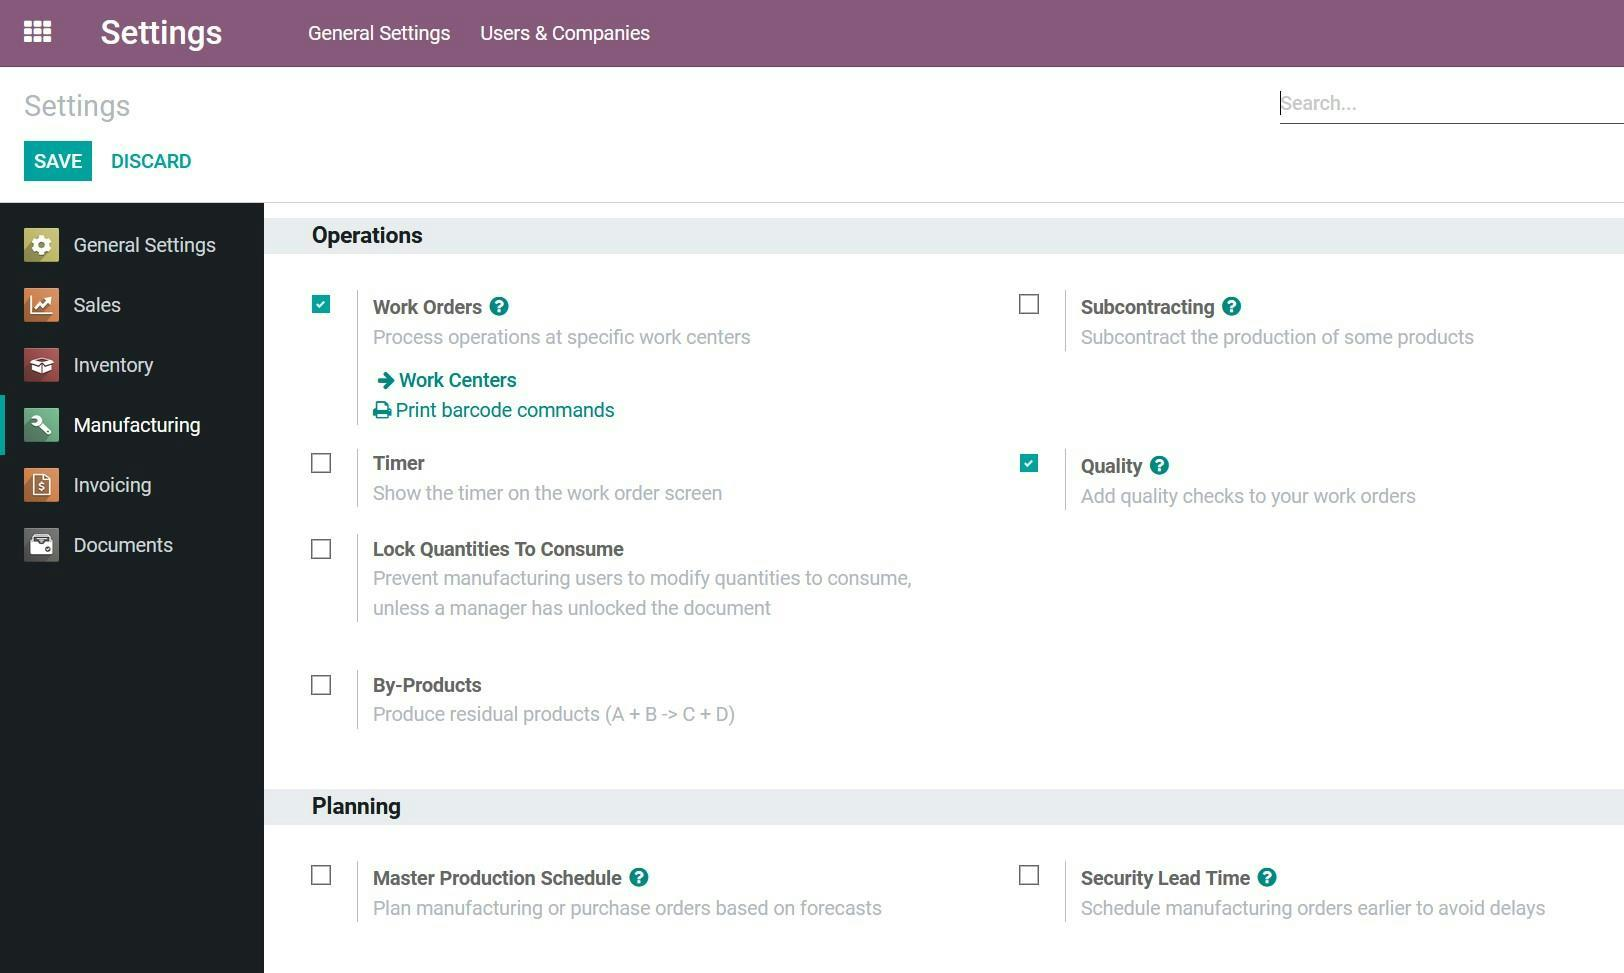
\includegraphics[width=441.9pt,height=264.75pt]{latexImage_52daeff2a6e63e4479395086cc469665.png}}
\end{picture}
\newpage
\begin{tikzpicture}[overlay]\path(0pt,0pt);\end{tikzpicture}
\begin{picture}(-5,0)(2.5,0)
\put(500.14,-727.616){\fontsize{12}{1}\usefont{T1}{ptm}{m}{n}\selectfont\color{color_29791}37}
\put(512.14,-727.616){\fontsize{12}{1}\usefont{T1}{ptm}{m}{n}\selectfont\color{color_29791} }
\put(515.14,-727.616){\fontsize{12}{1}\usefont{T1}{ptm}{m}{n}\selectfont\color{color_29791} }
\put(70.104,-742.496){\fontsize{10.56}{1}\usefont{T1}{ptm}{m}{n}\selectfont\color{color_29791} }
\put(72.744,-742.496){\fontsize{12}{1}\usefont{T1}{ptm}{m}{n}\selectfont\color{color_29791} }
\put(515.62,-447.15){\fontsize{12}{1}\usefont{T1}{ptm}{m}{n}\selectfont\color{color_29791} }
\put(242.81,-460.11){\fontsize{12}{1}\usefont{T1}{ptm}{m}{n}\selectfont\color{color_29791}圖}
\put(254.93,-460.11){\fontsize{12}{1}\usefont{T1}{ptm}{b}{n}\selectfont\color{color_29791}29}
\put(266.81,-460.11){\fontsize{12}{1}\usefont{T1}{ptm}{m}{n}\selectfont\color{color_29791}用戶介}
\put(302.918,-460.11){\fontsize{12}{1}\usefont{T1}{ptm}{m}{n}\selectfont\color{color_29791}面截圖}
\put(339.07,-460.11){\fontsize{12}{1}\usefont{T1}{ptm}{b}{n}\selectfont\color{color_29791} }
\put(341.95,-460.11){\fontsize{12}{1}\usefont{T1}{ptm}{m}{n}\selectfont\color{color_29791} }
\put(84.24,-75.43999){
\includegraphics[width=3.96pt,height=14.52pt]{latexImage_21dd4c4fcf795dc74410ea0ebd83af4a.png}}
\put(84.264,-72.09998){\fontsize{12}{1}\usefont{T1}{ptm}{m}{n}\selectfont\color{color_29791} }
\put(87.26,-72.09998){\fontsize{12}{1}\usefont{T1}{ptm}{m}{n}\selectfont\color{color_29791} }
\put(512.64,-450.68){
\includegraphics[width=3.96pt,height=14.52pt]{latexImage_21dd4c4fcf795dc74410ea0ebd83af4a.png}}
\put(512.74,-447.39){\fontsize{12}{1}\usefont{T1}{ptm}{m}{n}\selectfont\color{color_29791} }
\put(515.74,-447.39){\fontsize{12}{1}\usefont{T1}{ptm}{m}{n}\selectfont\color{color_29791} }
\put(70.05,-444.4399){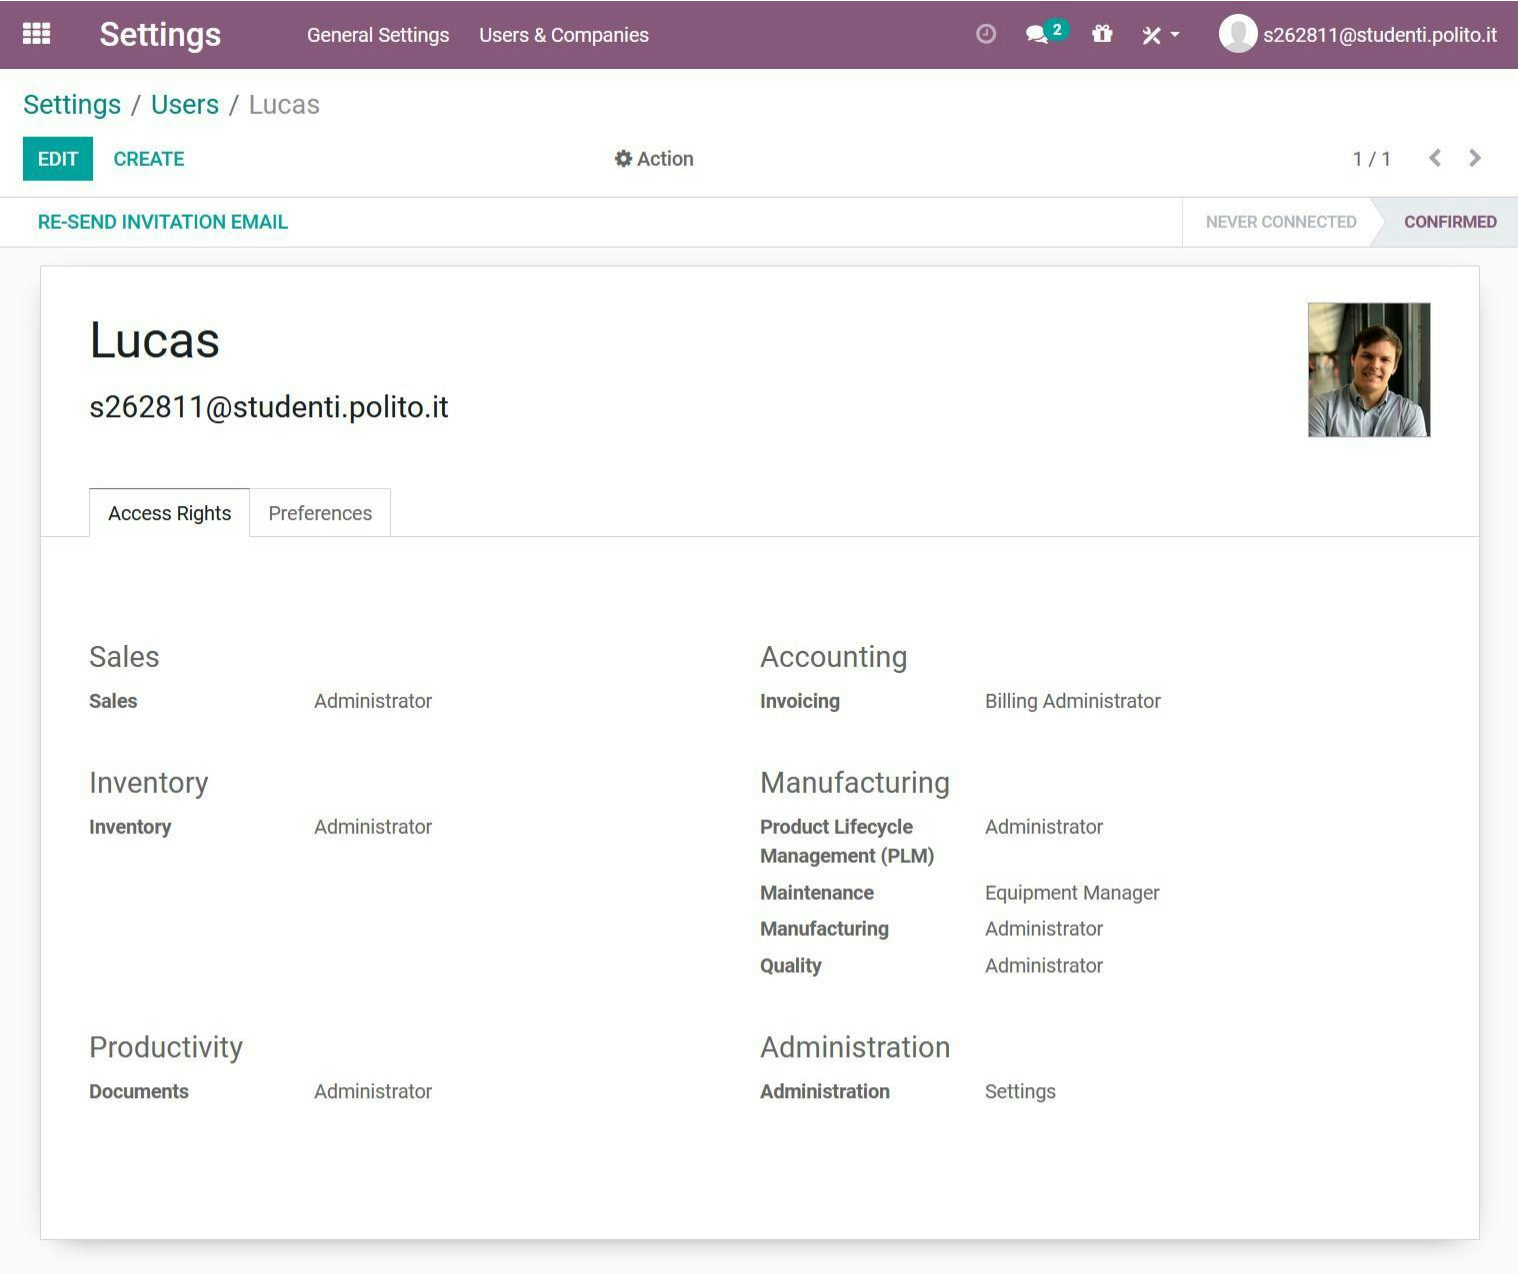
\includegraphics[width=441.88pt,height=370.59pt]{latexImage_b11e0eb10bbb8708e69fad69293b506f.png}}
\put(91.2,-201.92){
\includegraphics[width=114.95pt,height=16.92pt]{latexImage_c67913f8e34d93bd918ce0f2a51cfd62.png}}
\put(94.12,-197.2){
\includegraphics[width=109.2pt,height=11.28pt]{latexImage_34130a03975df4ab6ebf6f4e4092cc26.png}}
\put(434.02,-93.08){
\includegraphics[width=78.597pt,height=16.317pt]{latexImage_ef3c06c5ca02eb104b1283d8c7b4fc17.png}}
\put(437.38,-88.00002){
\includegraphics[width=71.997pt,height=9.8398pt]{latexImage_fd5ac5db0234b9f92cc07374c100c7b2.png}}
\end{picture}
\begin{tikzpicture}[overlay]
\path(0pt,0pt);
\draw[color_156992,line width=0.75pt,line join=round]
(437.73pt, -87.95001pt) -- (509.277pt, -87.95001pt)
 -- (509.277pt, -87.95001pt)
 -- (509.277pt, -78.7002pt)
 -- (509.277pt, -78.7002pt)
 -- (437.73pt, -78.7002pt) -- cycle
;
\end{tikzpicture}
\newpage
\begin{tikzpicture}[overlay]\path(0pt,0pt);\end{tikzpicture}
\begin{picture}(-5,0)(2.5,0)
\put(500.14,-727.616){\fontsize{12}{1}\usefont{T1}{ptm}{m}{n}\selectfont\color{color_29791}38}
\put(512.14,-727.616){\fontsize{12}{1}\usefont{T1}{ptm}{m}{n}\selectfont\color{color_29791} }
\put(515.14,-727.616){\fontsize{12}{1}\usefont{T1}{ptm}{m}{n}\selectfont\color{color_29791} }
\put(70.104,-742.496){\fontsize{10.56}{1}\usefont{T1}{ptm}{m}{n}\selectfont\color{color_29791} }
\put(72.744,-742.496){\fontsize{12}{1}\usefont{T1}{ptm}{m}{n}\selectfont\color{color_29791} }
\put(511.3,-354.61){\fontsize{12}{1}\usefont{T1}{ptm}{m}{n}\selectfont\color{color_29791} }
\put(514.3,-354.61){\fontsize{12}{1}\usefont{T1}{ptm}{m}{n}\selectfont\color{color_29791} }
\put(217.25,-367.09){\fontsize{12}{1}\usefont{T1}{ptm}{m}{n}\selectfont\color{color_29791}圖}
\put(229.37,-367.09){\fontsize{12}{1}\usefont{T1}{ptm}{b}{n}\selectfont\color{color_29791}30 }
\put(244.25,-367.09){\fontsize{12}{1}\usefont{T1}{ptm}{m}{n}\selectfont\color{color_29791}第二個}
\put(280.358,-367.09){\fontsize{12}{1}\usefont{T1}{ptm}{m}{n}\selectfont\color{color_29791}使用者介面截圖}
\put(364.51,-367.09){\fontsize{12}{1}\usefont{T1}{ptm}{b}{n}\selectfont\color{color_29791} }
\put(367.39,-367.09){\fontsize{12}{1}\usefont{T1}{ptm}{m}{n}\selectfont\color{color_29791} }
\put(70.104,-384.37){\fontsize{12}{1}\usefont{T1}{ptm}{m}{n}\selectfont\color{color_29791} }
\put(73.104,-384.37){\fontsize{12}{1}\usefont{T1}{ptm}{m}{n}\selectfont\color{color_29791} }
\put(87.38,-399.49){\fontsize{12}{1}\usefont{T1}{ptm}{m}{n}\selectfont\color{color_29791}很高興指出兩者在訪問許可權上的不同之處}
\put(315.43,-399.49){\fontsize{12}{1}\usefont{T1}{ptm}{m}{n}\selectfont\color{color_29791}。}
\put(327.43,-399.49){\fontsize{12}{1}\usefont{T1}{ptm}{m}{n}\selectfont\color{color_29791}在此示例中}
\put(387.43,-399.49){\fontsize{12}{1}\usefont{T1}{ptm}{m}{n}\selectfont\color{color_29791},}
\put(399.43,-399.49){\fontsize{12}{1}\usefont{T1}{ptm}{m}{n}\selectfont\color{color_29791}Ma}
\put(415.39,-399.49){\fontsize{12}{1}\usefont{T1}{ptm}{m}{n}\selectfont\color{color_29791}r}
\put(419.578,-399.49){\fontsize{12}{1}\usefont{T1}{ptm}{m}{n}\selectfont\color{color_29791}y}
\put(425.458,-399.49){\fontsize{12}{1}\usefont{T1}{ptm}{m}{n}\selectfont\color{color_29791} }
\put(478.606,-399.49){\fontsize{12}{1}\usefont{T1}{ptm}{m}{n}\selectfont\color{color_29791}F}
\put(485.206,-399.49){\fontsize{12}{1}\usefont{T1}{ptm}{m}{n}\selectfont\color{color_29791}iction}
\put(512.446,-399.49){\fontsize{12}{1}\usefont{T1}{ptm}{m}{n}\selectfont\color{color_29791} }
\put(69.384,-417.13){\fontsize{12}{1}\usefont{T1}{ptm}{m}{n}\selectfont\color{color_29791}是以工程師身份創建的}
\put(189.41,-417.13){\fontsize{12}{1}\usefont{T1}{ptm}{m}{n}\selectfont\color{color_29791},}
\put(201.41,-417.13){\fontsize{12}{1}\usefont{T1}{ptm}{m}{n}\selectfont\color{color_29791}因此她的大部分許可權都與製造程式有關}
\put(417.43,-417.13){\fontsize{12}{1}\usefont{T1}{ptm}{m}{n}\selectfont\color{color_29791},}
\put(429.43,-417.13){\fontsize{12}{1}\usefont{T1}{ptm}{m}{n}\selectfont\color{color_29791}而她則被拒絕}
\put(69.384,-434.79){\fontsize{12}{1}\usefont{T1}{ptm}{m}{n}\selectfont\color{color_29791}訪問其他部分}
\put(141.38,-434.79){\fontsize{12}{1}\usefont{T1}{ptm}{m}{n}\selectfont\color{color_29791},}
\put(153.38,-434.79){\fontsize{12}{1}\usefont{T1}{ptm}{m}{n}\selectfont\color{color_29791}例如銷售或會計}
\put(237.41,-434.79){\fontsize{12}{1}\usefont{T1}{ptm}{m}{n}\selectfont\color{color_29791}。}
\put(249.41,-434.79){\fontsize{12}{1}\usefont{T1}{ptm}{m}{n}\selectfont\color{color_29791}  }
\put(255.41,-434.79){\fontsize{12}{1}\usefont{T1}{ptm}{m}{n}\selectfont\color{color_29791} }
\put(105.38,-474.39){\fontsize{12.96}{1}\usefont{T1}{ptm}{b}{n}\selectfont\color{color_29791}5.3.2. }
\put(137.78,-474.39){\fontsize{12.96}{1}\usefont{T1}{ptm}{m}{n}\selectfont\color{color_29791}工}
\put(150.8437,-474.39){\fontsize{12.96}{1}\usefont{T1}{ptm}{m}{n}\selectfont\color{color_29791}作}
\put(163.9073,-474.39){\fontsize{12.96}{1}\usefont{T1}{ptm}{m}{n}\selectfont\color{color_29791}中}
\put(176.971,-474.39){\fontsize{12.96}{1}\usefont{T1}{ptm}{m}{n}\selectfont\color{color_29791}心和}
\put(202.9947,-474.39){\fontsize{12.96}{1}\usefont{T1}{ptm}{m}{n}\selectfont\color{color_29791}設備}
\put(229.13,-474.39){\fontsize{12.96}{1}\usefont{T1}{ptm}{b}{n}\selectfont\color{color_29791} }
\put(232.37,-474.39){\fontsize{12.96}{1}\usefont{T1}{ptm}{b}{n}\selectfont\color{color_29791} }
\put(82.944,-503.43){\fontsize{12}{1}\usefont{T1}{ptm}{m}{n}\selectfont\color{color_29791}工作中心在}
\put(142.94,-503.43){\fontsize{12}{1}\usefont{T1}{ptm}{m}{n}\selectfont\color{color_29791}Odoo}
\put(169.58,-503.43){\fontsize{12}{1}\usefont{T1}{ptm}{m}{n}\selectfont\color{color_29791}中非常靈活}
\put(229.61,-503.43){\fontsize{12}{1}\usefont{T1}{ptm}{m}{n}\selectfont\color{color_29791},}
\put(241.61,-503.43){\fontsize{12}{1}\usefont{T1}{ptm}{m}{n}\selectfont\color{color_29791}可以根據需要進行更改和擴展}
\put(397.63,-503.43){\fontsize{12}{1}\usefont{T1}{ptm}{m}{n}\selectfont\color{color_29791}。}
\put(409.63,-503.43){\fontsize{12}{1}\usefont{T1}{ptm}{m}{n}\selectfont\color{color_29791}可以在創建產品專}
\put(69.384,-520.95){\fontsize{12}{1}\usefont{T1}{ptm}{m}{n}\selectfont\color{color_29791}案后創建工作中心}
\put(165.38,-520.95){\fontsize{12}{1}\usefont{T1}{ptm}{m}{n}\selectfont\color{color_29791},}
\put(177.38,-520.95){\fontsize{12}{1}\usefont{T1}{ptm}{m}{n}\selectfont\color{color_29791}以便在您對產品最終將是什麼有所瞭解后對車間進行重組}
\put(477.46,-520.95){\fontsize{12}{1}\usefont{T1}{ptm}{m}{n}\selectfont\color{color_29791}。}
\put(489.46,-520.95){\fontsize{12}{1}\usefont{T1}{ptm}{m}{n}\selectfont\color{color_29791}然}
\put(69.384,-538.59){\fontsize{12}{1}\usefont{T1}{ptm}{m}{n}\selectfont\color{color_29791}而}
\put(81.384,-538.59){\fontsize{12}{1}\usefont{T1}{ptm}{m}{n}\selectfont\color{color_29791},}
\put(93.38,-538.59){\fontsize{12}{1}\usefont{T1}{ptm}{m}{n}\selectfont\color{color_29791}對於大多數情況來說}
\put(201.41,-538.59){\fontsize{12}{1}\usefont{T1}{ptm}{m}{n}\selectfont\color{color_29791},}
\put(213.41,-538.59){\fontsize{12}{1}\usefont{T1}{ptm}{m}{n}\selectfont\color{color_29791}這似乎是不現實的}
\put(309.41,-538.59){\fontsize{12}{1}\usefont{T1}{ptm}{m}{n}\selectfont\color{color_29791},}
\put(321.43,-538.59){\fontsize{12}{1}\usefont{T1}{ptm}{m}{n}\selectfont\color{color_29791}因為工作中心在現實世界中是更嚴}
\put(69.384,-556.35){\fontsize{12}{1}\usefont{T1}{ptm}{m}{n}\selectfont\color{color_29791}格的結構}
\put(117.38,-556.35){\fontsize{12}{1}\usefont{T1}{ptm}{m}{n}\selectfont\color{color_29791}——}
\put(141.38,-556.35){\fontsize{12}{1}\usefont{T1}{ptm}{m}{n}\selectfont\color{color_29791}它們的變化不如產品}
\put(249.41,-556.35){\fontsize{12}{1}\usefont{T1}{ptm}{m}{n}\selectfont\color{color_29791},}
\put(261.41,-556.35){\fontsize{12}{1}\usefont{T1}{ptm}{m}{n}\selectfont\color{color_29791}因為它們往往容納重型機械}
\put(405.43,-556.35){\fontsize{12}{1}\usefont{T1}{ptm}{m}{n}\selectfont\color{color_29791}。}
\put(417.43,-556.35){\fontsize{12}{1}\usefont{T1}{ptm}{m}{n}\selectfont\color{color_29791}  }
\put(423.43,-556.35){\fontsize{12}{1}\usefont{T1}{ptm}{m}{n}\selectfont\color{color_29791} }
\put(84.264,-573.87){\fontsize{12}{1}\usefont{T1}{ptm}{m}{n}\selectfont\color{color_29791} }
\put(87.26,-573.87){\fontsize{12}{1}\usefont{T1}{ptm}{m}{n}\selectfont\color{color_29791} }
\put(82.944,-588.99){\fontsize{12}{1}\usefont{T1}{ptm}{m}{n}\selectfont\color{color_29791}在這個類比中}
\put(154.94,-588.99){\fontsize{12}{1}\usefont{T1}{ptm}{m}{n}\selectfont\color{color_29791},}
\put(166.94,-588.99){\fontsize{12}{1}\usefont{T1}{ptm}{m}{n}\selectfont\color{color_29791}我們認為該公司從一開始就已經有}
\put(346.99,-588.99){\fontsize{12}{1}\usefont{T1}{ptm}{m}{n}\selectfont\color{color_29791} }
\put(506.5,-588.99){\fontsize{12}{1}\usefont{T1}{ptm}{m}{n}\selectfont\color{color_29791}3 }
\put(69.384,-606.66){\fontsize{12}{1}\usefont{T1}{ptm}{m}{n}\selectfont\color{color_29791}個工作中心}
\put(129.38,-606.66){\fontsize{12}{1}\usefont{T1}{ptm}{m}{n}\selectfont\color{color_29791},}
\put(141.38,-606.66){\fontsize{12}{1}\usefont{T1}{ptm}{m}{n}\selectfont\color{color_29791}因此工作中心和機器是事先創建的}
\put(321.43,-606.66){\fontsize{12}{1}\usefont{T1}{ptm}{m}{n}\selectfont\color{color_29791}。}
\put(333.43,-606.66){\fontsize{12}{1}\usefont{T1}{ptm}{m}{n}\selectfont\color{color_29791}這對於有興趣實現}
\put(429.43,-606.66){\fontsize{12}{1}\usefont{T1}{ptm}{m}{n}\selectfont\color{color_29791}Odoo}
\put(456.1,-606.66){\fontsize{12}{1}\usefont{T1}{ptm}{m}{n}\selectfont\color{color_29791}並節省一}
\put(69.384,-624.42){\fontsize{12}{1}\usefont{T1}{ptm}{m}{n}\selectfont\color{color_29791}些時間的讀者來說更有用}
\put(201.41,-624.42){\fontsize{12}{1}\usefont{T1}{ptm}{m}{n}\selectfont\color{color_29791}。}
\put(213.41,-624.42){\fontsize{12}{1}\usefont{T1}{ptm}{m}{n}\selectfont\color{color_29791} }
\put(216.41,-624.42){\fontsize{12}{1}\usefont{T1}{ptm}{m}{n}\selectfont\color{color_29791} }
\put(84.264,-641.82){\fontsize{12}{1}\usefont{T1}{ptm}{m}{n}\selectfont\color{color_29791} }
\put(87.26,-641.82){\fontsize{12}{1}\usefont{T1}{ptm}{m}{n}\selectfont\color{color_29791} }
\put(82.944,-656.94){\fontsize{12}{1}\usefont{T1}{ptm}{m}{n}\selectfont\color{color_29791}我們從創建我們擁有的設備開始}
\put(250.97,-656.94){\fontsize{12}{1}\usefont{T1}{ptm}{m}{n}\selectfont\color{color_29791}。}
\put(262.97,-656.94){\fontsize{12}{1}\usefont{T1}{ptm}{m}{n}\selectfont\color{color_29791}這是維護組織中強調的項類}
\put(406.99,-656.94){\fontsize{12}{1}\usefont{T1}{ptm}{m}{n}\selectfont\color{color_29791}。}
\put(418.99,-656.94){\fontsize{12}{1}\usefont{T1}{ptm}{m}{n}\selectfont\color{color_29791}負責管理設備的}
\put(69.384,-674.7){\fontsize{12}{1}\usefont{T1}{ptm}{m}{n}\selectfont\color{color_29791}應用程式是維護應用程式}
\put(202.73,-674.7){\fontsize{12}{1}\usefont{T1}{ptm}{m}{n}\selectfont\color{color_29791}。}
\put(214.85,-674.7){\fontsize{12}{1}\usefont{T1}{ptm}{m}{n}\selectfont\color{color_29791}下圖是}
\put(251.21,-674.7){\fontsize{12}{1}\usefont{T1}{ptm}{m}{n}\selectfont\color{color_29791}O}
\put(259.958,-674.7){\fontsize{12}{1}\usefont{T1}{ptm}{m}{n}\selectfont\color{color_29791}d}
\put(266.066,-674.7){\fontsize{12}{1}\usefont{T1}{ptm}{m}{n}\selectfont\color{color_29791}o}
\put(272.174,-674.7){\fontsize{12}{1}\usefont{T1}{ptm}{m}{n}\selectfont\color{color_29791}o}
\put(278.33,-674.7){\fontsize{12}{1}\usefont{T1}{ptm}{m}{n}\selectfont\color{color_29791}如何描繪}
\put(326.83,-674.7){\fontsize{12}{1}\usefont{T1}{ptm}{m}{n}\selectfont\color{color_29791}3}
\put(332.95,-674.7){\fontsize{12}{1}\usefont{T1}{ptm}{m}{n}\selectfont\color{color_29791}D}
\put(341.71,-674.7){\fontsize{12}{1}\usefont{T1}{ptm}{m}{n}\selectfont\color{color_29791}印表機設備專案的示例}
\put(463.06,-674.7){\fontsize{12}{1}\usefont{T1}{ptm}{m}{n}\selectfont\color{color_29791}(}
\put(475.3,-674.7){\fontsize{12}{1}\usefont{T1}{ptm}{m}{n}\selectfont\color{color_29791}圖}
\put(487.54,-674.7){\fontsize{12}{1}\usefont{T1}{ptm}{m}{n}\selectfont\color{color_29791}31}
\put(500.02,-674.7){\fontsize{12}{1}\usefont{T1}{ptm}{m}{n}\selectfont\color{color_29791})。}
\put(524.5,-674.7){\fontsize{12}{1}\usefont{T1}{ptm}{m}{n}\selectfont\color{color_29791} }
\put(527.5,-674.7){\fontsize{12}{1}\usefont{T1}{ptm}{m}{n}\selectfont\color{color_29791} }
\put(73.3,-354.55){
\includegraphics[width=437.9pt,height=293.65pt]{latexImage_2db7bd18d94f8b86fca11206f4d0e720.png}}
\end{picture}
\newpage
\begin{tikzpicture}[overlay]\path(0pt,0pt);\end{tikzpicture}
\begin{picture}(-5,0)(2.5,0)
\put(500.14,-727.616){\fontsize{12}{1}\usefont{T1}{ptm}{m}{n}\selectfont\color{color_29791}39}
\put(512.14,-727.616){\fontsize{12}{1}\usefont{T1}{ptm}{m}{n}\selectfont\color{color_29791} }
\put(515.14,-727.616){\fontsize{12}{1}\usefont{T1}{ptm}{m}{n}\selectfont\color{color_29791} }
\put(70.104,-742.496){\fontsize{10.56}{1}\usefont{T1}{ptm}{m}{n}\selectfont\color{color_29791} }
\put(72.744,-742.496){\fontsize{12}{1}\usefont{T1}{ptm}{m}{n}\selectfont\color{color_29791} }
\put(515.74,-287.29){\fontsize{12}{1}\usefont{T1}{ptm}{m}{n}\selectfont\color{color_29791} }
\put(518.74,-287.29){\fontsize{12}{1}\usefont{T1}{ptm}{m}{n}\selectfont\color{color_29791} }
\put(214.01,-299.77){\fontsize{12}{1}\usefont{T1}{ptm}{m}{n}\selectfont\color{color_29791}圖}
\put(226.13,-299.77){\fontsize{12}{1}\usefont{T1}{ptm}{b}{n}\selectfont\color{color_29791}31 }
\put(241.13,-299.77){\fontsize{12}{1}\usefont{T1}{ptm}{b}{n}\selectfont\color{color_29791}Od}
\put(257.198,-299.77){\fontsize{12}{1}\usefont{T1}{ptm}{b}{n}\selectfont\color{color_29791}oo3D}
\put(283.73,-299.77){\fontsize{12}{1}\usefont{T1}{ptm}{m}{n}\selectfont\color{color_29791}印表機設備專案}
\put(367.87,-299.77){\fontsize{12}{1}\usefont{T1}{ptm}{b}{n}\selectfont\color{color_29791} }
\put(370.75,-299.77){\fontsize{12}{1}\usefont{T1}{ptm}{m}{n}\selectfont\color{color_29791} }
\put(70.104,-317.05){\fontsize{12}{1}\usefont{T1}{ptm}{m}{n}\selectfont\color{color_29791} }
\put(73.104,-317.05){\fontsize{12}{1}\usefont{T1}{ptm}{m}{n}\selectfont\color{color_29791} }
\put(82.944,-332.41){\fontsize{12}{1}\usefont{T1}{ptm}{m}{n}\selectfont\color{color_29791}除了這台}
\put(130.94,-332.41){\fontsize{12}{1}\usefont{T1}{ptm}{m}{n}\selectfont\color{color_29791} }
\put(136.1,-332.41){\fontsize{12}{1}\usefont{T1}{ptm}{m}{n}\selectfont\color{color_29791}3D }
\put(155.9,-332.41){\fontsize{12}{1}\usefont{T1}{ptm}{m}{n}\selectfont\color{color_29791}印表機之外}
\put(215.93,-332.41){\fontsize{12}{1}\usefont{T1}{ptm}{m}{n}\selectfont\color{color_29791},}
\put(227.93,-332.41){\fontsize{12}{1}\usefont{T1}{ptm}{m}{n}\selectfont\color{color_29791}還創建了以下設備}
\put(323.95,-332.41){\fontsize{12}{1}\usefont{T1}{ptm}{m}{n}\selectfont\color{color_29791},}
\put(335.95,-332.41){\fontsize{12}{1}\usefont{T1}{ptm}{m}{n}\selectfont\color{color_29791}用於整個開發}
\put(407.95,-332.41){\fontsize{12}{1}\usefont{T1}{ptm}{m}{n}\selectfont\color{color_29791}/}
\put(411.31,-332.41){\fontsize{12}{1}\usefont{T1}{ptm}{m}{n}\selectfont\color{color_29791}生產過程}
\put(459.34,-332.41){\fontsize{12}{1}\usefont{T1}{ptm}{m}{n}\selectfont\color{color_29791}(}
\put(471.34,-332.41){\fontsize{12}{1}\usefont{T1}{ptm}{m}{n}\selectfont\color{color_29791}圖}
\put(483.34,-332.41){\fontsize{12}{1}\usefont{T1}{ptm}{m}{n}\selectfont\color{color_29791} }
\put(488.5,-332.41){\fontsize{12}{1}\usefont{T1}{ptm}{m}{n}\selectfont\color{color_29791}32}
\put(500.5,-332.41){\fontsize{12}{1}\usefont{T1}{ptm}{m}{n}\selectfont\color{color_29791}):}
\put(524.5,-332.41){\fontsize{12}{1}\usefont{T1}{ptm}{m}{n}\selectfont\color{color_29791} }
\put(527.5,-332.41){\fontsize{12}{1}\usefont{T1}{ptm}{m}{n}\selectfont\color{color_29791} }
\put(84.264,-349.81){\fontsize{12}{1}\usefont{T1}{ptm}{m}{n}\selectfont\color{color_29791} }
\put(87.26,-349.81){\fontsize{12}{1}\usefont{T1}{ptm}{m}{n}\selectfont\color{color_29791} }
\put(515.74,-582.63){\fontsize{12}{1}\usefont{T1}{ptm}{m}{n}\selectfont\color{color_29791} }
\put(518.74,-582.63){\fontsize{12}{1}\usefont{T1}{ptm}{m}{n}\selectfont\color{color_29791} }
\put(242.93,-595.14){\fontsize{12}{1}\usefont{T1}{ptm}{m}{n}\selectfont\color{color_29791}圖}
\put(255.05,-595.14){\fontsize{12}{1}\usefont{T1}{ptm}{b}{n}\selectfont\color{color_29791}32}
\put(266.93,-595.14){\fontsize{12}{1}\usefont{T1}{ptm}{m}{n}\selectfont\color{color_29791}設備專}
\put(303.038,-595.14){\fontsize{12}{1}\usefont{T1}{ptm}{m}{n}\selectfont\color{color_29791}案概覽}
\put(339.19,-595.14){\fontsize{12}{1}\usefont{T1}{ptm}{b}{n}\selectfont\color{color_29791} }
\put(342.07,-595.14){\fontsize{12}{1}\usefont{T1}{ptm}{m}{n}\selectfont\color{color_29791} }
\put(70.104,-612.54){\fontsize{12}{1}\usefont{T1}{ptm}{m}{n}\selectfont\color{color_29791} }
\put(73.104,-612.54){\fontsize{12}{1}\usefont{T1}{ptm}{m}{n}\selectfont\color{color_29791} }
\put(82.944,-627.66){\fontsize{12}{1}\usefont{T1}{ptm}{m}{n}\selectfont\color{color_29791}這就是有關}
\put(142.94,-627.66){\fontsize{12}{1}\usefont{T1}{ptm}{m}{n}\selectfont\color{color_29791} }
\put(487.78,-627.66){\fontsize{12}{1}\usefont{T1}{ptm}{m}{n}\selectfont\color{color_29791}P}
\put(494.608,-627.66){\fontsize{12}{1}\usefont{T1}{ptm}{m}{n}\selectfont\color{color_29791}L}
\put(501.688,-627.66){\fontsize{12}{1}\usefont{T1}{ptm}{m}{n}\selectfont\color{color_29791}M}
\put(512.476,-627.66){\fontsize{12}{1}\usefont{T1}{ptm}{m}{n}\selectfont\color{color_29791} }
\put(69.384,-645.3){\fontsize{12}{1}\usefont{T1}{ptm}{m}{n}\selectfont\color{color_29791}的軟體限制開始顯現的地方}
\put(213.41,-645.3){\fontsize{12}{1}\usefont{T1}{ptm}{m}{n}\selectfont\color{color_29791}。}
\put(225.41,-645.3){\fontsize{12}{1}\usefont{T1}{ptm}{m}{n}\selectfont\color{color_29791}儘管設備專案允許您使用某種級別的元數據}
\put(453.46,-645.3){\fontsize{12}{1}\usefont{T1}{ptm}{m}{n}\selectfont\color{color_29791}(}
\put(465.46,-645.3){\fontsize{12}{1}\usefont{T1}{ptm}{m}{n}\selectfont\color{color_29791}描述文}
\put(69.384,-662.94){\fontsize{12}{1}\usefont{T1}{ptm}{m}{n}\selectfont\color{color_29791}本}
\put(81.384,-662.94){\fontsize{12}{1}\usefont{T1}{ptm}{m}{n}\selectfont\color{color_29791}、}
\put(93.38,-662.94){\fontsize{12}{1}\usefont{T1}{ptm}{m}{n}\selectfont\color{color_29791}負責使用者}
\put(153.38,-662.94){\fontsize{12}{1}\usefont{T1}{ptm}{m}{n}\selectfont\color{color_29791}、}
\put(165.38,-662.94){\fontsize{12}{1}\usefont{T1}{ptm}{m}{n}\selectfont\color{color_29791}維護數據和供應商}
\put(261.41,-662.94){\fontsize{12}{1}\usefont{T1}{ptm}{m}{n}\selectfont\color{color_29791})。}
\put(285.41,-662.94){\fontsize{12}{1}\usefont{T1}{ptm}{m}{n}\selectfont\color{color_29791}它不允許上傳任何類型的檔附加到專案類}
\put(69.384,-680.46){\fontsize{12}{1}\usefont{T1}{ptm}{m}{n}\selectfont\color{color_29791}(}
\put(81.384,-680.46){\fontsize{12}{1}\usefont{T1}{ptm}{m}{n}\selectfont\color{color_29791}機器手冊}
\put(129.38,-680.46){\fontsize{12}{1}\usefont{T1}{ptm}{m}{n}\selectfont\color{color_29791}、}
\put(141.38,-680.46){\fontsize{12}{1}\usefont{T1}{ptm}{m}{n}\selectfont\color{color_29791}報告等}
\put(177.38,-680.46){\fontsize{12}{1}\usefont{T1}{ptm}{m}{n}\selectfont\color{color_29791})。}
\put(201.41,-680.46){\fontsize{12}{1}\usefont{T1}{ptm}{m}{n}\selectfont\color{color_29791}這是一個很大的弱點}
\put(309.41,-680.46){\fontsize{12}{1}\usefont{T1}{ptm}{m}{n}\selectfont\color{color_29791},}
\put(321.43,-680.46){\fontsize{12}{1}\usefont{T1}{ptm}{m}{n}\selectfont\color{color_29791}因為檔管理是人們一致認為是}
\put(477.46,-680.46){\fontsize{12}{1}\usefont{T1}{ptm}{m}{n}\selectfont\color{color_29791} }
\put(487.9,-680.46){\fontsize{12}{1}\usefont{T1}{ptm}{m}{n}\selectfont\color{color_29791}P}
\put(494.728,-680.46){\fontsize{12}{1}\usefont{T1}{ptm}{m}{n}\selectfont\color{color_29791}L}
\put(501.808,-680.46){\fontsize{12}{1}\usefont{T1}{ptm}{m}{n}\selectfont\color{color_29791}M }
\put(73.75,-287.25){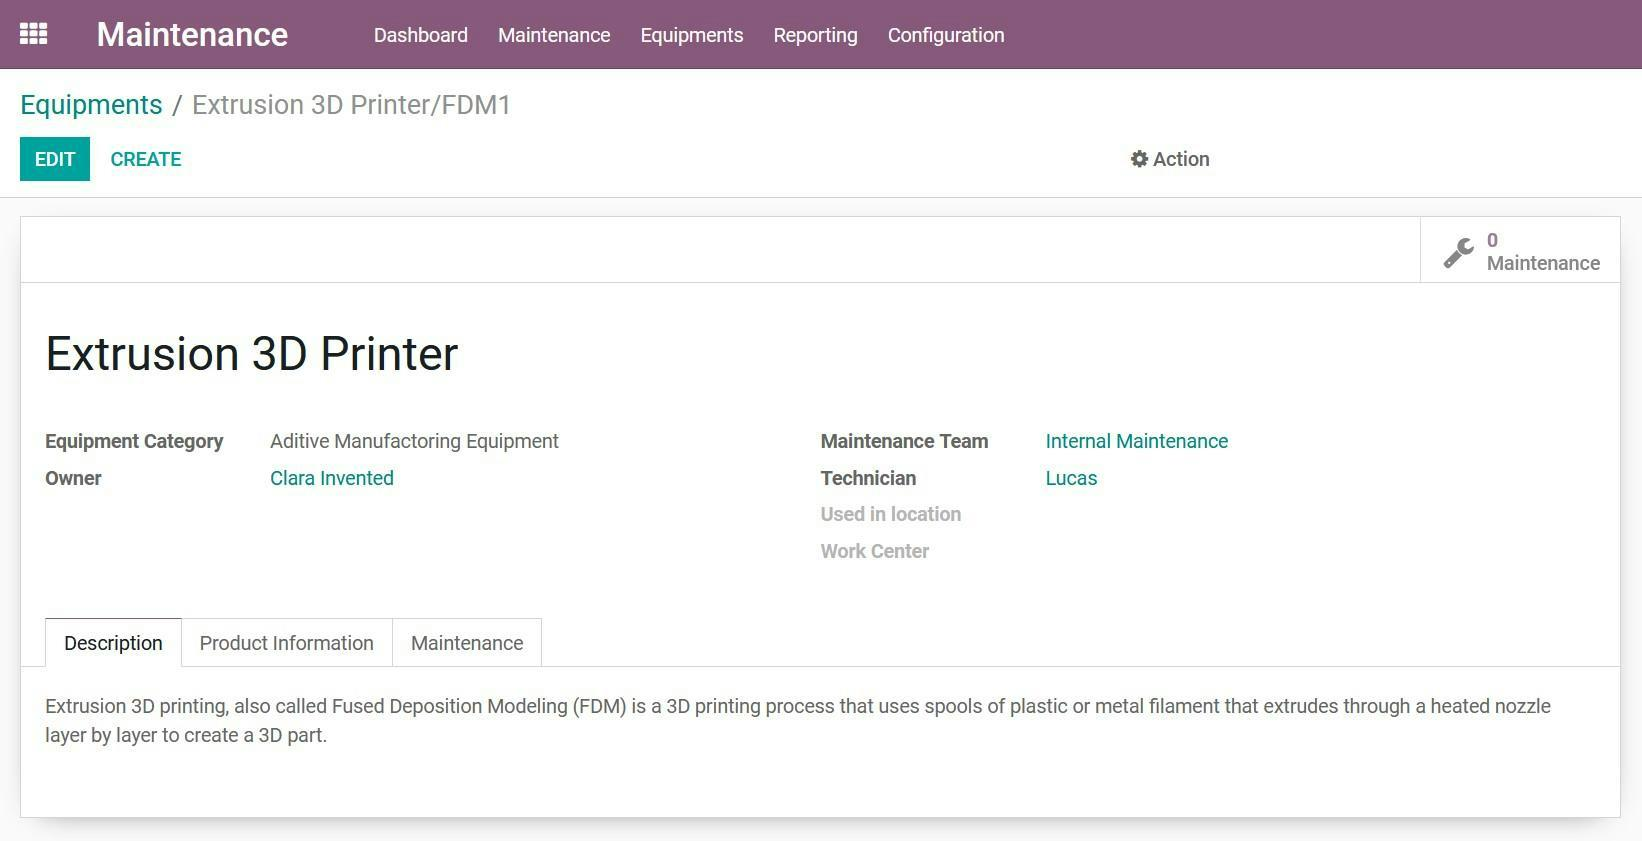
\includegraphics[width=441.9pt,height=226.35pt]{latexImage_09014630c2d3f28d84b8832fef6ca51c.png}}
\put(73.75,-582.6){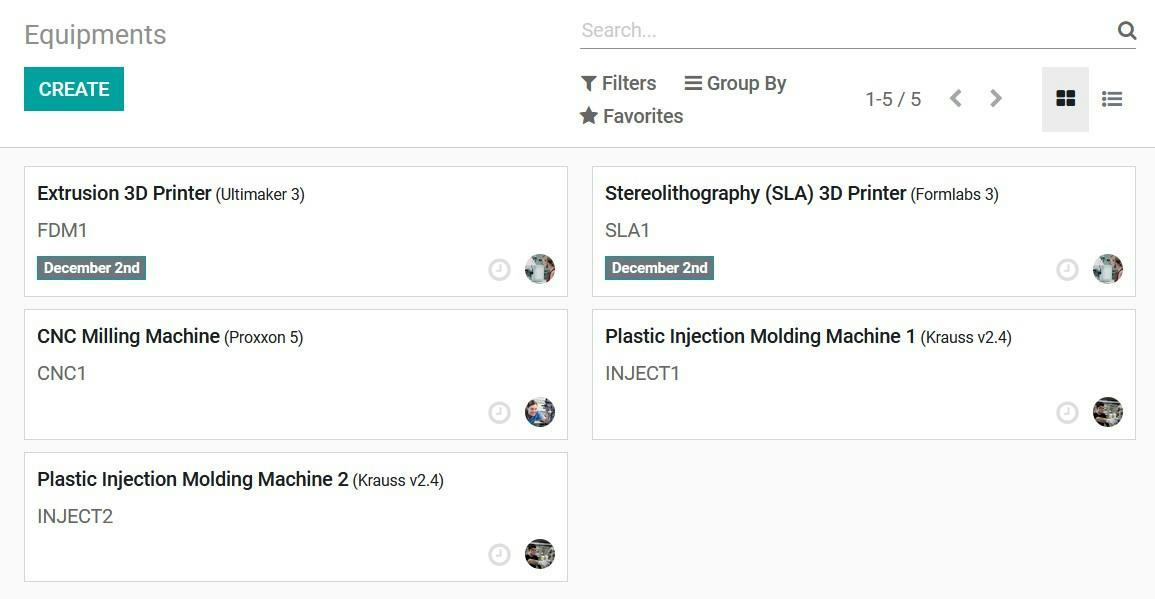
\includegraphics[width=441.9pt,height=229.1pt]{latexImage_216f3d0f6b2efb0e1ed4cd840af928a3.png}}
\end{picture}
\newpage
\begin{tikzpicture}[overlay]\path(0pt,0pt);\end{tikzpicture}
\begin{picture}(-5,0)(2.5,0)
\put(500.14,-727.616){\fontsize{12}{1}\usefont{T1}{ptm}{m}{n}\selectfont\color{color_29791}40}
\put(512.14,-727.616){\fontsize{12}{1}\usefont{T1}{ptm}{m}{n}\selectfont\color{color_29791} }
\put(515.14,-727.616){\fontsize{12}{1}\usefont{T1}{ptm}{m}{n}\selectfont\color{color_29791} }
\put(70.104,-742.496){\fontsize{10.56}{1}\usefont{T1}{ptm}{m}{n}\selectfont\color{color_29791} }
\put(72.744,-742.496){\fontsize{12}{1}\usefont{T1}{ptm}{m}{n}\selectfont\color{color_29791} }
\put(69.384,-72.34003){\fontsize{12}{1}\usefont{T1}{ptm}{m}{n}\selectfont\color{color_29791}的一個主要方面}
\put(153.38,-72.34003){\fontsize{12}{1}\usefont{T1}{ptm}{m}{n}\selectfont\color{color_29791}。}
\put(165.38,-72.34003){\fontsize{12}{1}\usefont{T1}{ptm}{m}{n}\selectfont\color{color_29791}這將是此類比中反覆出現的主題}
\put(333.43,-72.34003){\fontsize{12}{1}\usefont{T1}{ptm}{m}{n}\selectfont\color{color_29791},}
\put(345.43,-72.34003){\fontsize{12}{1}\usefont{T1}{ptm}{m}{n}\selectfont\color{color_29791}因為允許直接上傳檔的項目數}
\put(69.384,-90.09998){\fontsize{12}{1}\usefont{T1}{ptm}{m}{n}\selectfont\color{color_29791}量在}
\put(93.38,-90.09998){\fontsize{12}{1}\usefont{T1}{ptm}{m}{n}\selectfont\color{color_29791}Odoo}
\put(120.02,-90.09998){\fontsize{12}{1}\usefont{T1}{ptm}{m}{n}\selectfont\color{color_29791}中受到限制}
\put(180.05,-90.09998){\fontsize{12}{1}\usefont{T1}{ptm}{m}{n}\selectfont\color{color_29791}。}
\put(192.05,-90.09998){\fontsize{12}{1}\usefont{T1}{ptm}{m}{n}\selectfont\color{color_29791}  }
\put(198.05,-90.09998){\fontsize{12}{1}\usefont{T1}{ptm}{m}{n}\selectfont\color{color_29791} }
\put(70.104,-107.5){\fontsize{12}{1}\usefont{T1}{ptm}{m}{n}\selectfont\color{color_29791} }
\put(73.104,-107.5){\fontsize{12}{1}\usefont{T1}{ptm}{m}{n}\selectfont\color{color_29791} }
\put(82.944,-122.62){\fontsize{12}{1}\usefont{T1}{ptm}{m}{n}\selectfont\color{color_29791}現在設備已經創建}
\put(178.94,-122.62){\fontsize{12}{1}\usefont{T1}{ptm}{m}{n}\selectfont\color{color_29791},}
\put(190.97,-122.62){\fontsize{12}{1}\usefont{T1}{ptm}{m}{n}\selectfont\color{color_29791}可以創建他們的工作中心}
\put(322.99,-122.62){\fontsize{12}{1}\usefont{T1}{ptm}{m}{n}\selectfont\color{color_29791}。}
\put(334.99,-122.62){\fontsize{12}{1}\usefont{T1}{ptm}{m}{n}\selectfont\color{color_29791}有趣的是}
\put(382.99,-122.62){\fontsize{12}{1}\usefont{T1}{ptm}{m}{n}\selectfont\color{color_29791},}
\put(394.99,-122.62){\fontsize{12}{1}\usefont{T1}{ptm}{m}{n}\selectfont\color{color_29791}工作中心專案的主要}
\put(69.384,-140.26){\fontsize{12}{1}\usefont{T1}{ptm}{m}{n}\selectfont\color{color_29791}用途是管理每小時的時間和成本}
\put(237.41,-140.26){\fontsize{12}{1}\usefont{T1}{ptm}{m}{n}\selectfont\color{color_29791}。}
\put(249.41,-140.26){\fontsize{12}{1}\usefont{T1}{ptm}{m}{n}\selectfont\color{color_29791}這個想法是}
\put(309.41,-140.26){\fontsize{12}{1}\usefont{T1}{ptm}{m}{n}\selectfont\color{color_29791},}
\put(321.43,-140.26){\fontsize{12}{1}\usefont{T1}{ptm}{m}{n}\selectfont\color{color_29791}分配給廁所的設備不應同時使用}
\put(489.46,-140.26){\fontsize{12}{1}\usefont{T1}{ptm}{m}{n}\selectfont\color{color_29791},}
\put(69.384,-157.9){\fontsize{12}{1}\usefont{T1}{ptm}{m}{n}\selectfont\color{color_29791}理想情況下}
\put(129.38,-157.9){\fontsize{12}{1}\usefont{T1}{ptm}{m}{n}\selectfont\color{color_29791},}
\put(141.38,-157.9){\fontsize{12}{1}\usefont{T1}{ptm}{m}{n}\selectfont\color{color_29791}運行成本差}
\put(201.41,-157.9){\fontsize{12}{1}\usefont{T1}{ptm}{m}{n}\selectfont\color{color_29791}異很大的設備也應該位於不同的工作中心}
\put(417.43,-157.9){\fontsize{12}{1}\usefont{T1}{ptm}{m}{n}\selectfont\color{color_29791},}
\put(429.43,-157.9){\fontsize{12}{1}\usefont{T1}{ptm}{m}{n}\selectfont\color{color_29791}以便更好地跟}
\put(69.384,-175.66){\fontsize{12}{1}\usefont{T1}{ptm}{m}{n}\selectfont\color{color_29791}蹤時間}
\put(105.38,-175.66){\fontsize{12}{1}\usefont{T1}{ptm}{m}{n}\selectfont\color{color_29791}/}
\put(108.74,-175.66){\fontsize{12}{1}\usefont{T1}{ptm}{m}{n}\selectfont\color{color_29791}成本}
\put(132.74,-175.66){\fontsize{12}{1}\usefont{T1}{ptm}{m}{n}\selectfont\color{color_29791}。}
\put(144.74,-175.66){\fontsize{12}{1}\usefont{T1}{ptm}{m}{n}\selectfont\color{color_29791}  }
\put(150.74,-175.66){\fontsize{12}{1}\usefont{T1}{ptm}{m}{n}\selectfont\color{color_29791} }
\put(70.104,-193.18){\fontsize{12}{1}\usefont{T1}{ptm}{m}{n}\selectfont\color{color_29791} }
\put(73.104,-193.18){\fontsize{12}{1}\usefont{T1}{ptm}{m}{n}\selectfont\color{color_29791} }
\put(82.944,-208.3){\fontsize{12}{1}\usefont{T1}{ptm}{m}{n}\selectfont\color{color_29791}下面}
\put(106.94,-208.3){\fontsize{12}{1}\usefont{T1}{ptm}{m}{n}\selectfont\color{color_29791}(}
\put(118.94,-208.3){\fontsize{12}{1}\usefont{T1}{ptm}{m}{n}\selectfont\color{color_29791}圖}
\put(130.94,-208.3){\fontsize{12}{1}\usefont{T1}{ptm}{m}{n}\selectfont\color{color_29791} }
\put(69.384,-225.94){\fontsize{12}{1}\usefont{T1}{ptm}{m}{n}\selectfont\color{color_29791}33}
\put(81.384,-225.94){\fontsize{12}{1}\usefont{T1}{ptm}{m}{n}\selectfont\color{color_29791})}
\put(93.38,-225.94){\fontsize{12}{1}\usefont{T1}{ptm}{m}{n}\selectfont\color{color_29791}是一個工作中心專案的示例}
\put(237.41,-225.94){\fontsize{12}{1}\usefont{T1}{ptm}{m}{n}\selectfont\color{color_29791},}
\put(249.41,-225.94){\fontsize{12}{1}\usefont{T1}{ptm}{m}{n}\selectfont\color{color_29791}用於表示在整個產品開發過程中使用的原型製作}
\put(69.384,-243.58){\fontsize{12}{1}\usefont{T1}{ptm}{m}{n}\selectfont\color{color_29791}站}
\put(81.384,-243.58){\fontsize{12}{1}\usefont{T1}{ptm}{m}{n}\selectfont\color{color_29791}。}
\put(93.38,-243.58){\fontsize{12}{1}\usefont{T1}{ptm}{m}{n}\selectfont\color{color_29791}  }
\put(99.38,-243.58){\fontsize{12}{1}\usefont{T1}{ptm}{m}{n}\selectfont\color{color_29791} }
\put(515.62,-601.02){\fontsize{12}{1}\usefont{T1}{ptm}{m}{n}\selectfont\color{color_29791} }
\put(213.89,-625.98){\fontsize{12}{1}\usefont{T1}{ptm}{m}{n}\selectfont\color{color_29791}圖}
\put(226.01,-625.98){\fontsize{12}{1}\usefont{T1}{ptm}{b}{n}\selectfont\color{color_29791} }
\put(229.01,-625.98){\fontsize{12}{1}\usefont{T1}{ptm}{b}{n}\selectfont\color{color_29791}33 }
\put(244.01,-625.98){\fontsize{12}{1}\usefont{T1}{ptm}{b}{n}\selectfont\color{color_29791}Od}
\put(260.078,-625.98){\fontsize{12}{1}\usefont{T1}{ptm}{b}{n}\selectfont\color{color_29791}oo }
\put(274.97,-625.98){\fontsize{12}{1}\usefont{T1}{ptm}{m}{n}\selectfont\color{color_29791}原型站專案表示}
\put(359.11,-625.98){\fontsize{12}{1}\usefont{T1}{ptm}{b}{n}\selectfont\color{color_29791} }
\put(362.11,-625.98){\fontsize{12}{1}\usefont{T1}{ptm}{b}{n}\selectfont\color{color_29791}1 }
\put(370.99,-625.98){\fontsize{12}{1}\usefont{T1}{ptm}{m}{n}\selectfont\color{color_29791} }
\put(70.104,-643.26){\fontsize{12}{1}\usefont{T1}{ptm}{b}{n}\selectfont\color{color_29791} }
\put(73.104,-643.26){\fontsize{12}{1}\usefont{T1}{ptm}{m}{n}\selectfont\color{color_29791} }
\put(82.944,-658.38){\fontsize{12}{1}\usefont{T1}{ptm}{m}{n}\selectfont\color{color_29791}讀者會注意到這個工作站}
\put(214.97,-658.38){\fontsize{12}{1}\usefont{T1}{ptm}{m}{n}\selectfont\color{color_29791}(}
\put(226.97,-658.38){\fontsize{12}{1}\usefont{T1}{ptm}{m}{n}\selectfont\color{color_29791}圖}
\put(238.97,-658.38){\fontsize{12}{1}\usefont{T1}{ptm}{m}{n}\selectfont\color{color_29791} }
\put(276.53,-658.38){\fontsize{12}{1}\usefont{T1}{ptm}{m}{n}\selectfont\color{color_29791}34}
\put(288.53,-658.38){\fontsize{12}{1}\usefont{T1}{ptm}{m}{n}\selectfont\color{color_29791})}
\put(300.53,-658.38){\fontsize{12}{1}\usefont{T1}{ptm}{m}{n}\selectfont\color{color_29791}是}
\put(312.55,-658.38){\fontsize{12}{1}\usefont{T1}{ptm}{m}{n}\selectfont\color{color_29791} }
\put(350.11,-658.38){\fontsize{12}{1}\usefont{T1}{ptm}{m}{n}\selectfont\color{color_29791}3D }
\put(402.31,-658.38){\fontsize{12}{1}\usefont{T1}{ptm}{m}{n}\selectfont\color{color_29791}印表機和}
\put(450.34,-658.38){\fontsize{12}{1}\usefont{T1}{ptm}{m}{n}\selectfont\color{color_29791} }
\put(487.9,-658.38){\fontsize{12}{1}\usefont{T1}{ptm}{m}{n}\selectfont\color{color_29791}C}
\put(495.928,-658.38){\fontsize{12}{1}\usefont{T1}{ptm}{m}{n}\selectfont\color{color_29791}NC}
\put(512.488,-658.38){\fontsize{12}{1}\usefont{T1}{ptm}{m}{n}\selectfont\color{color_29791} }
\put(69.384,-676.02){\fontsize{12}{1}\usefont{T1}{ptm}{m}{n}\selectfont\color{color_29791}機床所在的位置}
\put(153.38,-676.02){\fontsize{12}{1}\usefont{T1}{ptm}{m}{n}\selectfont\color{color_29791}。}
\put(165.38,-676.02){\fontsize{12}{1}\usefont{T1}{ptm}{m}{n}\selectfont\color{color_29791}通常}
\put(189.41,-676.02){\fontsize{12}{1}\usefont{T1}{ptm}{m}{n}\selectfont\color{color_29791},}
\put(201.41,-676.02){\fontsize{12}{1}\usefont{T1}{ptm}{m}{n}\selectfont\color{color_29791}由於運營成本的差異}
\put(309.41,-676.02){\fontsize{12}{1}\usefont{T1}{ptm}{m}{n}\selectfont\color{color_29791},}
\put(321.43,-676.02){\fontsize{12}{1}\usefont{T1}{ptm}{m}{n}\selectfont\color{color_29791}這些機器將分散在單個工作中心中}
\put(84.24,-264.44){
\includegraphics[width=3.96pt,height=14.52pt]{latexImage_21dd4c4fcf795dc74410ea0ebd83af4a.png}}
\put(84.264,-261.13){\fontsize{12}{1}\usefont{T1}{ptm}{m}{n}\selectfont\color{color_29791} }
\put(87.26,-261.13){\fontsize{12}{1}\usefont{T1}{ptm}{m}{n}\selectfont\color{color_29791} }
\put(512.64,-604.52){
\includegraphics[width=3.96pt,height=14.52pt]{latexImage_21dd4c4fcf795dc74410ea0ebd83af4a.png}}
\put(512.74,-601.26){\fontsize{12}{1}\usefont{T1}{ptm}{m}{n}\selectfont\color{color_29791} }
\put(515.74,-601.26){\fontsize{12}{1}\usefont{T1}{ptm}{m}{n}\selectfont\color{color_29791} }
\put(70.05,-598.08){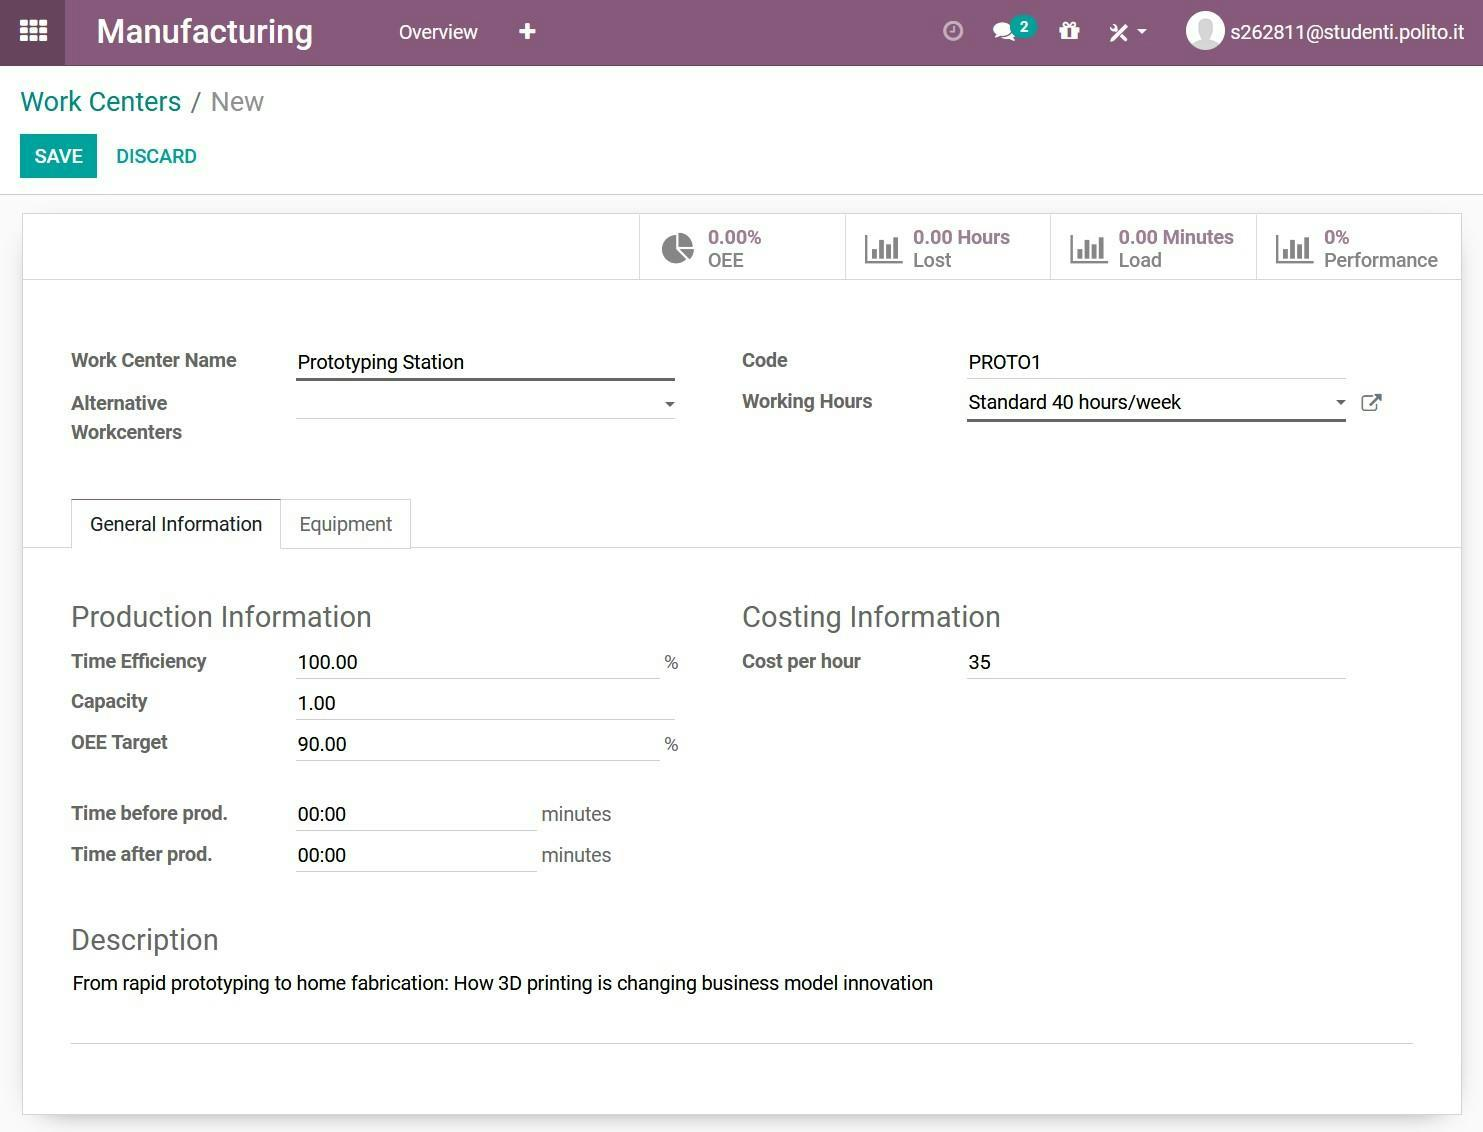
\includegraphics[width=441.88pt,height=337.26pt]{latexImage_7421ed300e3f4b81e32d182016f737cb.png}}
\put(433.06,-280.05){
\includegraphics[width=78.717pt,height=16.315pt]{latexImage_735cf46d81e0b7a65bc293b697365e45.png}}
\put(436.34,-274.89){
\includegraphics[width=72.237pt,height=9.5987pt]{latexImage_e4173eebe50c7c9ad6ce678705d30d18.png}}
\end{picture}
\begin{tikzpicture}[overlay]
\path(0pt,0pt);
\draw[color_156992,line width=0.75pt,line join=round]
(436.83pt, -274.92pt) -- (508.377pt, -274.92pt)
 -- (508.377pt, -274.92pt)
 -- (508.377pt, -265.6712pt)
 -- (508.377pt, -265.6712pt)
 -- (436.83pt, -265.6712pt) -- cycle
;
\end{tikzpicture}
\newpage
\begin{tikzpicture}[overlay]\path(0pt,0pt);\end{tikzpicture}
\begin{picture}(-5,0)(2.5,0)
\put(500.14,-727.616){\fontsize{12}{1}\usefont{T1}{ptm}{m}{n}\selectfont\color{color_29791}41}
\put(512.14,-727.616){\fontsize{12}{1}\usefont{T1}{ptm}{m}{n}\selectfont\color{color_29791} }
\put(515.14,-727.616){\fontsize{12}{1}\usefont{T1}{ptm}{m}{n}\selectfont\color{color_29791} }
\put(70.104,-742.496){\fontsize{10.56}{1}\usefont{T1}{ptm}{m}{n}\selectfont\color{color_29791} }
\put(72.744,-742.496){\fontsize{12}{1}\usefont{T1}{ptm}{m}{n}\selectfont\color{color_29791} }
\put(69.384,-72.34003){\fontsize{12}{1}\usefont{T1}{ptm}{m}{n}\selectfont\color{color_29791},}
\put(81.384,-72.34003){\fontsize{12}{1}\usefont{T1}{ptm}{m}{n}\selectfont\color{color_29791}並且因為它們在很大程度上是獨立的}
\put(273.41,-72.34003){\fontsize{12}{1}\usefont{T1}{ptm}{m}{n}\selectfont\color{color_29791},}
\put(285.41,-72.34003){\fontsize{12}{1}\usefont{T1}{ptm}{m}{n}\selectfont\color{color_29791}但是}
\put(309.41,-72.34003){\fontsize{12}{1}\usefont{T1}{ptm}{m}{n}\selectfont\color{color_29791},}
\put(321.43,-72.34003){\fontsize{12}{1}\usefont{T1}{ptm}{m}{n}\selectfont\color{color_29791}為了這種類比}
\put(393.43,-72.34003){\fontsize{12}{1}\usefont{T1}{ptm}{m}{n}\selectfont\color{color_29791},}
\put(405.43,-72.34003){\fontsize{12}{1}\usefont{T1}{ptm}{m}{n}\selectfont\color{color_29791}這被認為具有足夠}
\put(69.384,-90.09998){\fontsize{12}{1}\usefont{T1}{ptm}{m}{n}\selectfont\color{color_29791}的代表性}
\put(117.38,-90.09998){\fontsize{12}{1}\usefont{T1}{ptm}{m}{n}\selectfont\color{color_29791}。}
\put(129.38,-90.09998){\fontsize{12}{1}\usefont{T1}{ptm}{m}{n}\selectfont\color{color_29791}  }
\put(135.38,-90.09998){\fontsize{12}{1}\usefont{T1}{ptm}{m}{n}\selectfont\color{color_29791} }
\put(515.74,-327.73){\fontsize{12}{1}\usefont{T1}{ptm}{m}{n}\selectfont\color{color_29791} }
\put(518.74,-327.73){\fontsize{12}{1}\usefont{T1}{ptm}{m}{n}\selectfont\color{color_29791} }
\put(229.37,-340.33){\fontsize{12}{1}\usefont{T1}{ptm}{m}{n}\selectfont\color{color_29791}圖}
\put(241.49,-340.33){\fontsize{12}{1}\usefont{T1}{ptm}{b}{n}\selectfont\color{color_29791} }
\put(244.49,-340.33){\fontsize{12}{1}\usefont{T1}{ptm}{b}{n}\selectfont\color{color_29791}34 }
\put(259.37,-340.33){\fontsize{12}{1}\usefont{T1}{ptm}{m}{n}\selectfont\color{color_29791}原型站}
\put(295.478,-340.33){\fontsize{12}{1}\usefont{T1}{ptm}{m}{n}\selectfont\color{color_29791}專案表示}
\put(343.63,-340.33){\fontsize{12}{1}\usefont{T1}{ptm}{b}{n}\selectfont\color{color_29791} }
\put(346.51,-340.33){\fontsize{12}{1}\usefont{T1}{ptm}{b}{n}\selectfont\color{color_29791}2 }
\put(355.51,-340.33){\fontsize{12}{1}\usefont{T1}{ptm}{m}{n}\selectfont\color{color_29791} }
\put(70.104,-357.61){\fontsize{12}{1}\usefont{T1}{ptm}{m}{n}\selectfont\color{color_29791} }
\put(73.104,-357.61){\fontsize{12}{1}\usefont{T1}{ptm}{m}{n}\selectfont\color{color_29791} }
\put(82.944,-372.85){\fontsize{12}{1}\usefont{T1}{ptm}{m}{n}\selectfont\color{color_29791}還為類比創建了以下工作中心}
\put(238.97,-372.85){\fontsize{12}{1}\usefont{T1}{ptm}{m}{n}\selectfont\color{color_29791},}
\put(250.97,-372.85){\fontsize{12}{1}\usefont{T1}{ptm}{m}{n}\selectfont\color{color_29791}並配備了必要的設備}
\put(358.99,-372.85){\fontsize{12}{1}\usefont{T1}{ptm}{m}{n}\selectfont\color{color_29791}:}
\put(370.99,-372.85){\fontsize{12}{1}\usefont{T1}{ptm}{m}{n}\selectfont\color{color_29791}  }
\put(376.99,-372.85){\fontsize{12}{1}\usefont{T1}{ptm}{m}{n}\selectfont\color{color_29791} }
\put(70.104,-390.37){\fontsize{12}{1}\usefont{T1}{ptm}{m}{n}\selectfont\color{color_29791} }
\put(73.104,-390.37){\fontsize{12}{1}\usefont{T1}{ptm}{m}{n}\selectfont\color{color_29791} }
\put(508.3,-522.03){\fontsize{12}{1}\usefont{T1}{ptm}{m}{n}\selectfont\color{color_29791} }
\put(511.3,-522.03){\fontsize{12}{1}\usefont{T1}{ptm}{m}{n}\selectfont\color{color_29791} }
\put(225.77,-534.51){\fontsize{12}{1}\usefont{T1}{ptm}{m}{n}\selectfont\color{color_29791}圖}
\put(237.89,-534.51){\fontsize{12}{1}\usefont{T1}{ptm}{b}{n}\selectfont\color{color_29791} }
\put(240.89,-534.51){\fontsize{12}{1}\usefont{T1}{ptm}{b}{n}\selectfont\color{color_29791}35 }
\put(255.89,-534.51){\fontsize{12}{1}\usefont{T1}{ptm}{b}{n}\selectfont\color{color_29791}W}
\put(267.17,-534.51){\fontsize{12}{1}\usefont{T1}{ptm}{b}{n}\selectfont\color{color_29791}or}
\put(278.45,-534.51){\fontsize{12}{1}\usefont{T1}{ptm}{b}{n}\selectfont\color{color_29791}k}
\put(285.158,-534.51){\fontsize{12}{1}\usefont{T1}{ptm}{b}{n}\selectfont\color{color_29791}c}
\put(290.438,-534.51){\fontsize{12}{1}\usefont{T1}{ptm}{b}{n}\selectfont\color{color_29791}e}
\put(295.718,-534.51){\fontsize{12}{1}\usefont{T1}{ptm}{b}{n}\selectfont\color{color_29791}n}
\put(302.426,-534.51){\fontsize{12}{1}\usefont{T1}{ptm}{b}{n}\selectfont\color{color_29791}te}
\put(311.666,-534.51){\fontsize{12}{1}\usefont{T1}{ptm}{b}{n}\selectfont\color{color_29791}r}
\put(316.706,-534.51){\fontsize{12}{1}\usefont{T1}{ptm}{b}{n}\selectfont\color{color_29791} }
\put(319.75,-534.51){\fontsize{12}{1}\usefont{T1}{ptm}{m}{n}\selectfont\color{color_29791}項概述}
\put(356.11,-534.51){\fontsize{12}{1}\usefont{T1}{ptm}{b}{n}\selectfont\color{color_29791} }
\put(358.99,-534.51){\fontsize{12}{1}\usefont{T1}{ptm}{m}{n}\selectfont\color{color_29791} }
\put(70.104,-551.79){\fontsize{12}{1}\usefont{T1}{ptm}{m}{n}\selectfont\color{color_29791} }
\put(73.104,-551.79){\fontsize{12}{1}\usefont{T1}{ptm}{m}{n}\selectfont\color{color_29791} }
\put(87.38,-581.55){\fontsize{14.04}{1}\usefont{T1}{ptm}{b}{n}\selectfont\color{color_29791}5}
\put(94.44212,-581.55){\fontsize{14.04}{1}\usefont{T1}{ptm}{b}{n}\selectfont\color{color_29791}.4. }
\put(111.86,-581.55){\fontsize{14.04}{1}\usefont{T1}{ptm}{m}{n}\selectfont\color{color_29791}開發}
\put(140.06,-581.55){\fontsize{14.04}{1}\usefont{T1}{ptm}{b}{n}\selectfont\color{color_29791} }
\put(143.42,-581.55){\fontsize{14.04}{1}\usefont{T1}{ptm}{b}{n}\selectfont\color{color_29791} }
\put(82.944,-616.14){\fontsize{12}{1}\usefont{T1}{ptm}{m}{n}\selectfont\color{color_29791}現在}
\put(106.94,-616.14){\fontsize{12}{1}\usefont{T1}{ptm}{m}{n}\selectfont\color{color_29791},}
\put(118.94,-616.14){\fontsize{12}{1}\usefont{T1}{ptm}{m}{n}\selectfont\color{color_29791}公司的基本結構已在軟體中重新創建}
\put(310.97,-616.14){\fontsize{12}{1}\usefont{T1}{ptm}{m}{n}\selectfont\color{color_29791},}
\put(322.99,-616.14){\fontsize{12}{1}\usefont{T1}{ptm}{m}{n}\selectfont\color{color_29791}可以開始模擬過程}
\put(418.99,-616.14){\fontsize{12}{1}\usefont{T1}{ptm}{m}{n}\selectfont\color{color_29791}。}
\put(430.99,-616.14){\fontsize{12}{1}\usefont{T1}{ptm}{m}{n}\selectfont\color{color_29791}首先}
\put(455.02,-616.14){\fontsize{12}{1}\usefont{T1}{ptm}{m}{n}\selectfont\color{color_29791},}
\put(467.02,-616.14){\fontsize{12}{1}\usefont{T1}{ptm}{m}{n}\selectfont\color{color_29791}最引人}
\put(69.384,-633.66){\fontsize{12}{1}\usefont{T1}{ptm}{m}{n}\selectfont\color{color_29791}注目的是使用}
\put(141.38,-633.66){\fontsize{12}{1}\usefont{T1}{ptm}{m}{n}\selectfont\color{color_29791} }
\put(241.61,-633.66){\fontsize{12}{1}\usefont{T1}{ptm}{m}{n}\selectfont\color{color_29791}Odoo }
\put(368.47,-633.66){\fontsize{12}{1}\usefont{T1}{ptm}{m}{n}\selectfont\color{color_29791}的全新產品的開發方面}
\put(488.5,-633.66){\fontsize{12}{1}\usefont{T1}{ptm}{m}{n}\selectfont\color{color_29791}(}
\put(500.5,-633.66){\fontsize{12}{1}\usefont{T1}{ptm}{m}{n}\selectfont\color{color_29791}圖}
\put(512.5,-633.66){\fontsize{12}{1}\usefont{T1}{ptm}{m}{n}\selectfont\color{color_29791} }
\put(69.384,-651.3){\fontsize{12}{1}\usefont{T1}{ptm}{m}{n}\selectfont\color{color_29791}9}
\put(75.384,-651.3){\fontsize{12}{1}\usefont{T1}{ptm}{m}{n}\selectfont\color{color_29791}),}
\put(99.38,-651.3){\fontsize{12}{1}\usefont{T1}{ptm}{m}{n}\selectfont\color{color_29791}因為這是公司創建的第一款產品}
\put(267.41,-651.3){\fontsize{12}{1}\usefont{T1}{ptm}{m}{n}\selectfont\color{color_29791},}
\put(279.41,-651.3){\fontsize{12}{1}\usefont{T1}{ptm}{m}{n}\selectfont\color{color_29791}因此評估了}
\put(339.43,-651.3){\fontsize{12}{1}\usefont{T1}{ptm}{m}{n}\selectfont\color{color_29791} }
\put(485.86,-651.3){\fontsize{12}{1}\usefont{T1}{ptm}{m}{n}\selectfont\color{color_29791}Odoo }
\put(69.384,-668.94){\fontsize{12}{1}\usefont{T1}{ptm}{m}{n}\selectfont\color{color_29791}用於組織原型製作程式的可能性}
\put(237.41,-668.94){\fontsize{12}{1}\usefont{T1}{ptm}{m}{n}\selectfont\color{color_29791}。}
\put(249.41,-668.94){\fontsize{12}{1}\usefont{T1}{ptm}{m}{n}\selectfont\color{color_29791}這包括從構思到設計和原型生產的路徑}
\put(453.46,-668.94){\fontsize{12}{1}\usefont{T1}{ptm}{m}{n}\selectfont\color{color_29791}。}
\put(465.46,-668.94){\fontsize{12}{1}\usefont{T1}{ptm}{m}{n}\selectfont\color{color_29791}然後}
\put(489.46,-668.94){\fontsize{12}{1}\usefont{T1}{ptm}{m}{n}\selectfont\color{color_29791},}
\put(69.384,-686.576){\fontsize{12}{1}\usefont{T1}{ptm}{m}{n}\selectfont\color{color_29791}一旦產品作為原型達到可接受的結果}
\put(261.41,-686.576){\fontsize{12}{1}\usefont{T1}{ptm}{m}{n}\selectfont\color{color_29791},}
\put(273.41,-686.576){\fontsize{12}{1}\usefont{T1}{ptm}{m}{n}\selectfont\color{color_29791}就會進行有關生產過程開發的工作}
\put(453.46,-686.576){\fontsize{12}{1}\usefont{T1}{ptm}{m}{n}\selectfont\color{color_29791}。}
\put(465.46,-686.576){\fontsize{12}{1}\usefont{T1}{ptm}{m}{n}\selectfont\color{color_29791}一旦正}
\put(69.384,-704.336){\fontsize{12}{1}\usefont{T1}{ptm}{m}{n}\selectfont\color{color_29791}式生產運行完成}
\put(153.38,-704.336){\fontsize{12}{1}\usefont{T1}{ptm}{m}{n}\selectfont\color{color_29791},}
\put(165.38,-704.336){\fontsize{12}{1}\usefont{T1}{ptm}{m}{n}\selectfont\color{color_29791}產品開發就被認為是成功的}
\put(309.41,-704.336){\fontsize{12}{1}\usefont{T1}{ptm}{m}{n}\selectfont\color{color_29791}。}
\put(321.43,-704.336){\fontsize{12}{1}\usefont{T1}{ptm}{m}{n}\selectfont\color{color_29791} }
\put(324.43,-704.336){\fontsize{12}{1}\usefont{T1}{ptm}{m}{n}\selectfont\color{color_29791} }
\put(73.75,-327.75){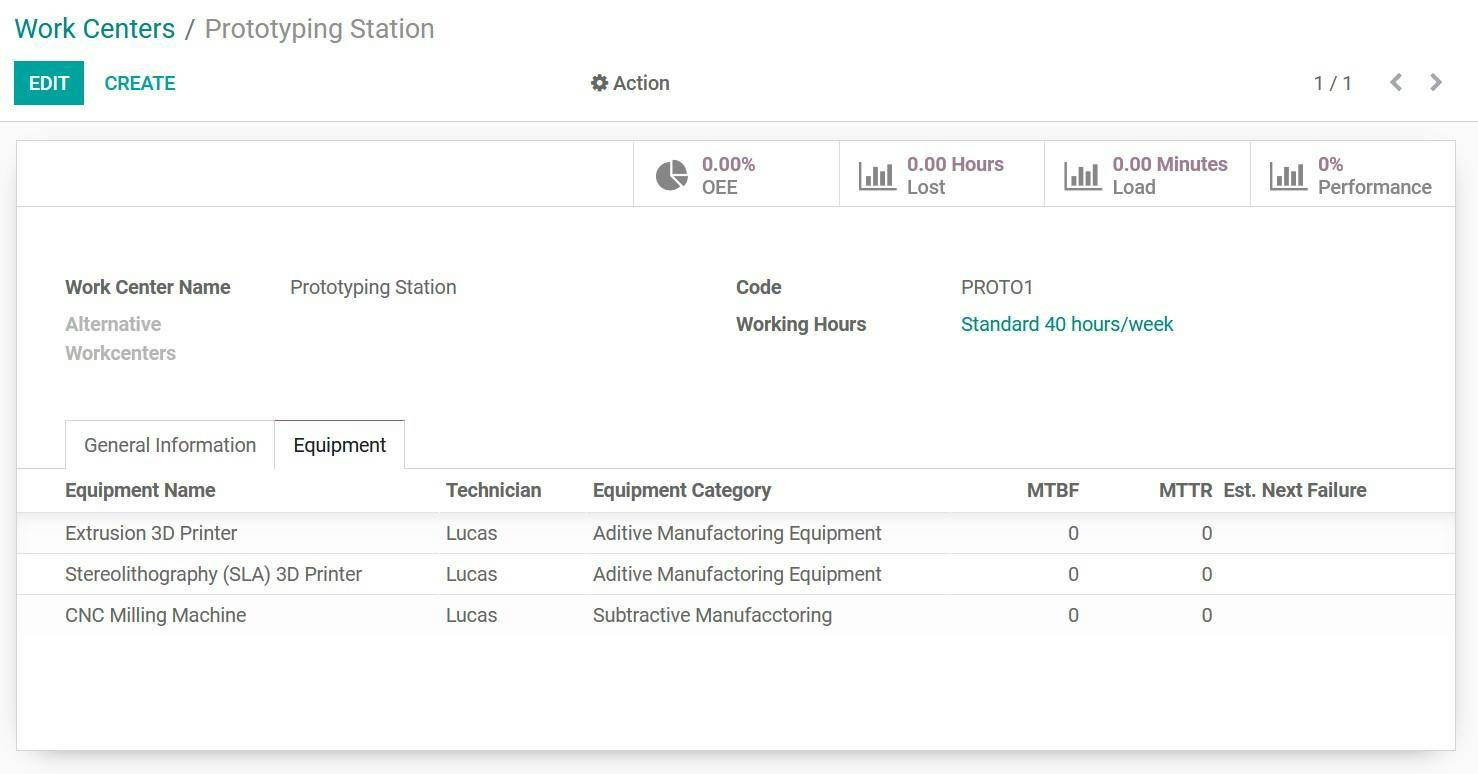
\includegraphics[width=441.9pt,height=231.4pt]{latexImage_cf476323ef4e6ac7161a0aecde24291e.png}}
\put(73.2,-521.9){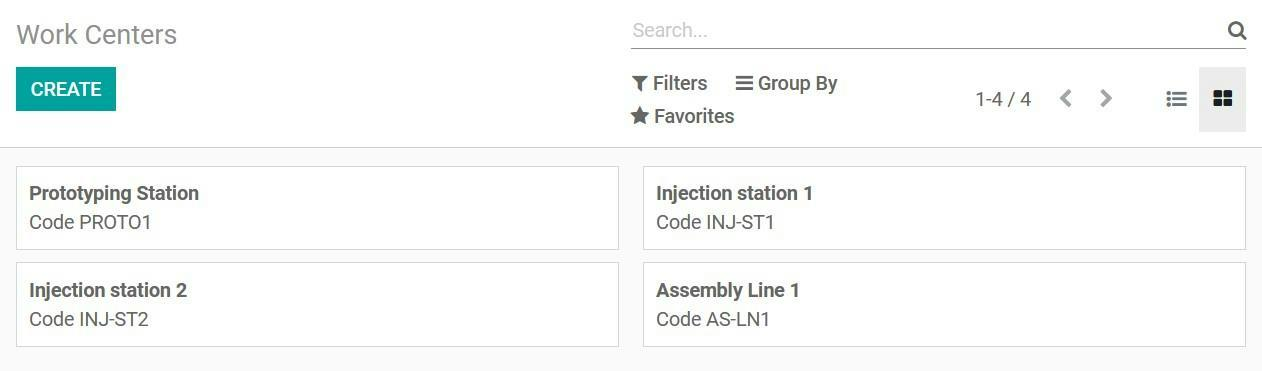
\includegraphics[width=435pt,height=127.9pt]{latexImage_0301d009d3bb7c4b734075914e38c0a4.png}}
\end{picture}
\newpage
\begin{tikzpicture}[overlay]\path(0pt,0pt);\end{tikzpicture}
\begin{picture}(-5,0)(2.5,0)
\put(500.14,-727.616){\fontsize{12}{1}\usefont{T1}{ptm}{m}{n}\selectfont\color{color_29791}42}
\put(512.14,-727.616){\fontsize{12}{1}\usefont{T1}{ptm}{m}{n}\selectfont\color{color_29791} }
\put(515.14,-727.616){\fontsize{12}{1}\usefont{T1}{ptm}{m}{n}\selectfont\color{color_29791} }
\put(70.104,-742.496){\fontsize{10.56}{1}\usefont{T1}{ptm}{m}{n}\selectfont\color{color_29791} }
\put(72.744,-742.496){\fontsize{12}{1}\usefont{T1}{ptm}{m}{n}\selectfont\color{color_29791} }
\put(70.104,-72.09998){\fontsize{12}{1}\usefont{T1}{ptm}{m}{n}\selectfont\color{color_29791} }
\put(73.104,-72.09998){\fontsize{12}{1}\usefont{T1}{ptm}{m}{n}\selectfont\color{color_29791} }
\put(105.38,-88.17999){\fontsize{12.96}{1}\usefont{T1}{ptm}{b}{n}\selectfont\color{color_29791}5.4.1. }
\put(137.78,-88.17999){\fontsize{12.96}{1}\usefont{T1}{ptm}{m}{n}\selectfont\color{color_29791}創意}
\put(163.94,-88.17999){\fontsize{12.96}{1}\usefont{T1}{ptm}{b}{n}\selectfont\color{color_29791} }
\put(167.18,-88.17999){\fontsize{12.96}{1}\usefont{T1}{ptm}{b}{n}\selectfont\color{color_29791}-}
\put(171.5,-88.17999){\fontsize{12.96}{1}\usefont{T1}{ptm}{b}{n}\selectfont\color{color_29791} }
\put(174.74,-88.17999){\fontsize{12.96}{1}\usefont{T1}{ptm}{m}{n}\selectfont\color{color_29791}設計}
\put(200.93,-88.17999){\fontsize{12.96}{1}\usefont{T1}{ptm}{b}{n}\selectfont\color{color_29791} }
\put(204.17,-88.17999){\fontsize{12.96}{1}\usefont{T1}{ptm}{b}{n}\selectfont\color{color_29791}-}
\put(208.49,-88.17999){\fontsize{12.96}{1}\usefont{T1}{ptm}{b}{n}\selectfont\color{color_29791} }
\put(211.73,-88.17999){\fontsize{12.96}{1}\usefont{T1}{ptm}{m}{n}\selectfont\color{color_29791}產品}
\put(237.7537,-88.17999){\fontsize{12.96}{1}\usefont{T1}{ptm}{m}{n}\selectfont\color{color_29791}原型}
\put(263.81,-88.17999){\fontsize{12.96}{1}\usefont{T1}{ptm}{b}{n}\selectfont\color{color_29791} }
\put(266.93,-88.17999){\fontsize{12.96}{1}\usefont{T1}{ptm}{b}{n}\selectfont\color{color_29791} }
\put(82.944,-117.1){\fontsize{12}{1}\usefont{T1}{ptm}{m}{n}\selectfont\color{color_29791}如}
\put(94.94,-117.1){\fontsize{12}{1}\usefont{T1}{ptm}{m}{n}\selectfont\color{color_29791}(}
\put(106.94,-117.1){\fontsize{12}{1}\usefont{T1}{ptm}{m}{n}\selectfont\color{color_29791}第}
\put(118.94,-117.1){\fontsize{12}{1}\usefont{T1}{ptm}{m}{n}\selectfont\color{color_29791}4}
\put(124.94,-117.1){\fontsize{12}{1}\usefont{T1}{ptm}{m}{n}\selectfont\color{color_29791}章}
\put(136.94,-117.1){\fontsize{12}{1}\usefont{T1}{ptm}{m}{n}\selectfont\color{color_29791})}
\put(148.94,-117.1){\fontsize{12}{1}\usefont{T1}{ptm}{m}{n}\selectfont\color{color_29791}所述}
\put(172.94,-117.1){\fontsize{12}{1}\usefont{T1}{ptm}{m}{n}\selectfont\color{color_29791},}
\put(184.97,-117.1){\fontsize{12}{1}\usefont{T1}{ptm}{m}{n}\selectfont\color{color_29791}產品的想法已經確定}
\put(292.97,-117.1){\fontsize{12}{1}\usefont{T1}{ptm}{m}{n}\selectfont\color{color_29791},}
\put(304.97,-117.1){\fontsize{12}{1}\usefont{T1}{ptm}{m}{n}\selectfont\color{color_29791}初步的設計特徵和基礎產品研究已經進}
\put(69.384,-134.74){\fontsize{12}{1}\usefont{T1}{ptm}{m}{n}\selectfont\color{color_29791}行}
\put(81.384,-134.74){\fontsize{12}{1}\usefont{T1}{ptm}{m}{n}\selectfont\color{color_29791}。}
\put(93.38,-134.74){\fontsize{12}{1}\usefont{T1}{ptm}{m}{n}\selectfont\color{color_29791}這代表了}
\put(141.38,-134.74){\fontsize{12}{1}\usefont{T1}{ptm}{m}{n}\selectfont\color{color_29791}Odoo}
\put(168.02,-134.74){\fontsize{12}{1}\usefont{T1}{ptm}{m}{n}\selectfont\color{color_29791}軟體在現實世界中的實際實施}
\put(324.07,-134.74){\fontsize{12}{1}\usefont{T1}{ptm}{m}{n}\selectfont\color{color_29791},}
\put(336.07,-134.74){\fontsize{12}{1}\usefont{T1}{ptm}{m}{n}\selectfont\color{color_29791}因為儘管}
\put(384.07,-134.74){\fontsize{12}{1}\usefont{T1}{ptm}{m}{n}\selectfont\color{color_29791}Odoo}
\put(410.71,-134.74){\fontsize{12}{1}\usefont{T1}{ptm}{m}{n}\selectfont\color{color_29791}具有良好的專案管}
\put(69.384,-152.38){\fontsize{12}{1}\usefont{T1}{ptm}{m}{n}\selectfont\color{color_29791}理和通信應用程式}
\put(165.38,-152.38){\fontsize{12}{1}\usefont{T1}{ptm}{m}{n}\selectfont\color{color_29791},}
\put(177.38,-152.38){\fontsize{12}{1}\usefont{T1}{ptm}{m}{n}\selectfont\color{color_29791}但這些應用程式是庫存和製造應用程式的外部}
\put(417.43,-152.38){\fontsize{12}{1}\usefont{T1}{ptm}{m}{n}\selectfont\color{color_29791},}
\put(429.43,-152.38){\fontsize{12}{1}\usefont{T1}{ptm}{m}{n}\selectfont\color{color_29791}更重要的是}
\put(489.46,-152.38){\fontsize{12}{1}\usefont{T1}{ptm}{m}{n}\selectfont\color{color_29791},}
\put(69.384,-170.02){\fontsize{12}{1}\usefont{T1}{ptm}{m}{n}\selectfont\color{color_29791}與工程設計}
\put(129.38,-170.02){\fontsize{12}{1}\usefont{T1}{ptm}{m}{n}\selectfont\color{color_29791}C}
\put(137.408,-170.02){\fontsize{12}{1}\usefont{T1}{ptm}{m}{n}\selectfont\color{color_29791}AD}
\put(154.7,-170.02){\fontsize{12}{1}\usefont{T1}{ptm}{m}{n}\selectfont\color{color_29791}軟體沒有集成}
\put(226.73,-170.02){\fontsize{12}{1}\usefont{T1}{ptm}{m}{n}\selectfont\color{color_29791}。}
\put(238.73,-170.02){\fontsize{12}{1}\usefont{T1}{ptm}{m}{n}\selectfont\color{color_29791}在這個類比中}
\put(310.73,-170.02){\fontsize{12}{1}\usefont{T1}{ptm}{m}{n}\selectfont\color{color_29791},}
\put(322.75,-170.02){\fontsize{12}{1}\usefont{T1}{ptm}{m}{n}\selectfont\color{color_29791}這個想法已經付諸實踐}
\put(442.75,-170.02){\fontsize{12}{1}\usefont{T1}{ptm}{m}{n}\selectfont\color{color_29791},}
\put(454.78,-170.02){\fontsize{12}{1}\usefont{T1}{ptm}{m}{n}\selectfont\color{color_29791}並使用}
\put(490.78,-170.02){\fontsize{12}{1}\usefont{T1}{ptm}{m}{n}\selectfont\color{color_29791} }
\put(69.384,-187.78){\fontsize{12}{1}\usefont{T1}{ptm}{m}{n}\selectfont\color{color_29791}S}
\put(76.092,-187.78){\fontsize{12}{1}\usefont{T1}{ptm}{m}{n}\selectfont\color{color_29791}oli}
\put(88.8,-187.78){\fontsize{12}{1}\usefont{T1}{ptm}{m}{n}\selectfont\color{color_29791}dwor}
\put(113.4,-187.78){\fontsize{12}{1}\usefont{T1}{ptm}{m}{n}\selectfont\color{color_29791}ks }
\put(127.1,-187.78){\fontsize{12}{1}\usefont{T1}{ptm}{m}{n}\selectfont\color{color_29791}軟體轉化為}
\put(187.13,-187.78){\fontsize{12}{1}\usefont{T1}{ptm}{m}{n}\selectfont\color{color_29791} }
\put(190.13,-187.78){\fontsize{12}{1}\usefont{T1}{ptm}{m}{n}\selectfont\color{color_29791}C}
\put(198.158,-187.78){\fontsize{12}{1}\usefont{T1}{ptm}{m}{n}\selectfont\color{color_29791}AD}
\put(215.438,-187.78){\fontsize{12}{1}\usefont{T1}{ptm}{m}{n}\selectfont\color{color_29791} }
\put(218.45,-187.78){\fontsize{12}{1}\usefont{T1}{ptm}{m}{n}\selectfont\color{color_29791}設計}
\put(242.45,-187.78){\fontsize{12}{1}\usefont{T1}{ptm}{m}{n}\selectfont\color{color_29791},}
\put(254.45,-187.78){\fontsize{12}{1}\usefont{T1}{ptm}{m}{n}\selectfont\color{color_29791}生成本地存儲在工程師計算機中的}
\put(434.47,-187.78){\fontsize{12}{1}\usefont{T1}{ptm}{m}{n}\selectfont\color{color_29791} }
\put(437.47,-187.78){\fontsize{12}{1}\usefont{T1}{ptm}{m}{n}\selectfont\color{color_29791}C}
\put(445.498,-187.78){\fontsize{12}{1}\usefont{T1}{ptm}{m}{n}\selectfont\color{color_29791}AD}
\put(462.778,-187.78){\fontsize{12}{1}\usefont{T1}{ptm}{m}{n}\selectfont\color{color_29791} }
\put(465.82,-187.78){\fontsize{12}{1}\usefont{T1}{ptm}{m}{n}\selectfont\color{color_29791}檔}
\put(477.82,-187.78){\fontsize{12}{1}\usefont{T1}{ptm}{m}{n}\selectfont\color{color_29791}。}
\put(489.82,-187.78){\fontsize{12}{1}\usefont{T1}{ptm}{m}{n}\selectfont\color{color_29791} }
\put(492.82,-187.78){\fontsize{12}{1}\usefont{T1}{ptm}{m}{n}\selectfont\color{color_29791} }
\put(84.264,-205.3){\fontsize{12}{1}\usefont{T1}{ptm}{m}{n}\selectfont\color{color_29791} }
\put(87.26,-205.3){\fontsize{12}{1}\usefont{T1}{ptm}{m}{n}\selectfont\color{color_29791} }
\put(398.35,-315.61){\fontsize{12}{1}\usefont{T1}{ptm}{m}{n}\selectfont\color{color_29791} }
\put(401.35,-315.61){\fontsize{12}{1}\usefont{T1}{ptm}{m}{n}\selectfont\color{color_29791} }
\put(230.93,-336.13){\fontsize{12}{1}\usefont{T1}{ptm}{m}{n}\selectfont\color{color_29791}圖}
\put(243.05,-336.13){\fontsize{12}{1}\usefont{T1}{ptm}{b}{n}\selectfont\color{color_29791}36}
\put(254.93,-336.13){\fontsize{12}{1}\usefont{T1}{ptm}{m}{n}\selectfont\color{color_29791}產品開}
\put(291.038,-336.13){\fontsize{12}{1}\usefont{T1}{ptm}{m}{n}\selectfont\color{color_29791}發的剖面圖}
\put(351.07,-336.13){\fontsize{12}{1}\usefont{T1}{ptm}{b}{n}\selectfont\color{color_29791} }
\put(354.07,-336.13){\fontsize{12}{1}\usefont{T1}{ptm}{m}{n}\selectfont\color{color_29791} }
\put(70.104,-353.41){\fontsize{12}{1}\usefont{T1}{ptm}{b}{n}\selectfont\color{color_29791}  }
\put(76.104,-353.41){\fontsize{12}{1}\usefont{T1}{ptm}{m}{n}\selectfont\color{color_29791} }
\put(82.944,-368.53){\fontsize{12}{1}\usefont{T1}{ptm}{m}{n}\selectfont\color{color_29791}正是在這一點上}
\put(166.94,-368.53){\fontsize{12}{1}\usefont{T1}{ptm}{m}{n}\selectfont\color{color_29791},}
\put(178.94,-368.53){\fontsize{12}{1}\usefont{T1}{ptm}{m}{n}\selectfont\color{color_29791}Odoo}
\put(205.61,-368.53){\fontsize{12}{1}\usefont{T1}{ptm}{m}{n}\selectfont\color{color_29791}軟體的正式使用可以正式發生}
\put(361.63,-368.53){\fontsize{12}{1}\usefont{T1}{ptm}{m}{n}\selectfont\color{color_29791}。}
\put(373.63,-368.53){\fontsize{12}{1}\usefont{T1}{ptm}{m}{n}\selectfont\color{color_29791}第一步是瞭解就產品專案}
\put(69.384,-386.29){\fontsize{12}{1}\usefont{T1}{ptm}{m}{n}\selectfont\color{color_29791}而言}
\put(93.38,-386.29){\fontsize{12}{1}\usefont{T1}{ptm}{m}{n}\selectfont\color{color_29791},}
\put(105.38,-386.29){\fontsize{12}{1}\usefont{T1}{ptm}{m}{n}\selectfont\color{color_29791}生產主題是什麼}
\put(189.41,-386.29){\fontsize{12}{1}\usefont{T1}{ptm}{m}{n}\selectfont\color{color_29791}。}
\put(201.41,-386.29){\fontsize{12}{1}\usefont{T1}{ptm}{m}{n}\selectfont\color{color_29791}如何做到這一點有兩種方法}
\put(345.43,-386.29){\fontsize{12}{1}\usefont{T1}{ptm}{m}{n}\selectfont\color{color_29791}:}
\put(357.43,-386.29){\fontsize{12}{1}\usefont{T1}{ptm}{m}{n}\selectfont\color{color_29791} }
\put(360.43,-386.29){\fontsize{12}{1}\usefont{T1}{ptm}{m}{n}\selectfont\color{color_29791} }
\put(84.264,-403.81){\fontsize{12}{1}\usefont{T1}{ptm}{m}{n}\selectfont\color{color_29791} }
\put(87.26,-403.81){\fontsize{12}{1}\usefont{T1}{ptm}{m}{n}\selectfont\color{color_29791} }
\put(105.14,-418.95){\fontsize{12}{1}\usefont{T1}{ptm}{m}{n}\selectfont\color{color_29791}}
\put(115.82,-418.95){\fontsize{12}{1}\usefont{T1}{uarial}{m}{n}\selectfont\color{color_29791} }
\put(123.14,-418.95){\fontsize{12}{1}\usefont{T1}{ptm}{m}{n}\selectfont\color{color_29791}第一種是將原型視為最終產品的早期修訂版}
\put(351.19,-418.95){\fontsize{12}{1}\usefont{T1}{ptm}{m}{n}\selectfont\color{color_29791},}
\put(363.19,-418.95){\fontsize{12}{1}\usefont{T1}{ptm}{m}{n}\selectfont\color{color_29791}也就是說}
\put(411.19,-418.95){\fontsize{12}{1}\usefont{T1}{ptm}{m}{n}\selectfont\color{color_29791},}
\put(423.19,-418.95){\fontsize{12}{1}\usefont{T1}{ptm}{m}{n}\selectfont\color{color_29791}在}
\put(435.19,-418.95){\fontsize{12}{1}\usefont{T1}{ptm}{m}{n}\selectfont\color{color_29791}Odoo}
\put(461.86,-418.95){\fontsize{12}{1}\usefont{T1}{ptm}{m}{n}\selectfont\color{color_29791}中創建的}
\put(123.14,-436.59){\fontsize{12}{1}\usefont{T1}{ptm}{m}{n}\selectfont\color{color_29791}原型專案將與最終產品專案相同}
\put(291.17,-436.59){\fontsize{12}{1}\usefont{T1}{ptm}{m}{n}\selectfont\color{color_29791},}
\put(303.17,-436.59){\fontsize{12}{1}\usefont{T1}{ptm}{m}{n}\selectfont\color{color_29791}並在開發過程中進行了修改}
\put(447.22,-436.59){\fontsize{12}{1}\usefont{T1}{ptm}{m}{n}\selectfont\color{color_29791}。}
\put(459.22,-436.59){\fontsize{12}{1}\usefont{T1}{ptm}{m}{n}\selectfont\color{color_29791}如果原型}
\put(123.14,-454.23){\fontsize{12}{1}\usefont{T1}{ptm}{m}{n}\selectfont\color{color_29791}是通過與最終生產中使用的方法相同的方法實現的}
\put(387.19,-454.23){\fontsize{12}{1}\usefont{T1}{ptm}{m}{n}\selectfont\color{color_29791},}
\put(399.19,-454.23){\fontsize{12}{1}\usefont{T1}{ptm}{m}{n}\selectfont\color{color_29791}則建議這樣做}
\put(471.22,-454.23){\fontsize{12}{1}\usefont{T1}{ptm}{m}{n}\selectfont\color{color_29791}。}
\put(483.22,-454.23){\fontsize{12}{1}\usefont{T1}{ptm}{m}{n}\selectfont\color{color_29791}這種}
\put(123.14,-471.87){\fontsize{12}{1}\usefont{T1}{ptm}{m}{n}\selectfont\color{color_29791}方法的一個例子是}
\put(219.17,-471.87){\fontsize{12}{1}\usefont{T1}{ptm}{m}{n}\selectfont\color{color_29791},}
\put(231.17,-471.87){\fontsize{12}{1}\usefont{T1}{ptm}{m}{n}\selectfont\color{color_29791}如果產品足夠簡單}
\put(327.19,-471.87){\fontsize{12}{1}\usefont{T1}{ptm}{m}{n}\selectfont\color{color_29791},}
\put(339.19,-471.87){\fontsize{12}{1}\usefont{T1}{ptm}{m}{n}\selectfont\color{color_29791}可以同時進行產品和生產方面的}
\put(123.14,-489.63){\fontsize{12}{1}\usefont{T1}{ptm}{m}{n}\selectfont\color{color_29791}開發}
\put(147.14,-489.63){\fontsize{12}{1}\usefont{T1}{ptm}{m}{n}\selectfont\color{color_29791}。}
\put(159.14,-489.63){\fontsize{12}{1}\usefont{T1}{ptm}{m}{n}\selectfont\color{color_29791} }
\put(162.14,-489.63){\fontsize{12}{1}\usefont{T1}{ptm}{m}{n}\selectfont\color{color_29791} }
\put(70.104,-507.03){\fontsize{12}{1}\usefont{T1}{ptm}{m}{n}\selectfont\color{color_29791} }
\put(73.104,-507.03){\fontsize{12}{1}\usefont{T1}{ptm}{m}{n}\selectfont\color{color_29791} }
\put(105.14,-522.15){\fontsize{12}{1}\usefont{T1}{ptm}{m}{n}\selectfont\color{color_29791}}
\put(115.82,-522.15){\fontsize{12}{1}\usefont{T1}{uarial}{m}{n}\selectfont\color{color_29791} }
\put(123.14,-522.15){\fontsize{12}{1}\usefont{T1}{ptm}{m}{n}\selectfont\color{color_29791}第二個是將原型視為與最終產品分開的專案}
\put(351.19,-522.15){\fontsize{12}{1}\usefont{T1}{ptm}{m}{n}\selectfont\color{color_29791} }
\put(508.54,-522.15){\fontsize{12}{1}\usefont{T1}{ptm}{m}{n}\selectfont\color{color_29791}-}
\put(512.5,-522.15){\fontsize{12}{1}\usefont{T1}{ptm}{m}{n}\selectfont\color{color_29791} }
\put(123.14,-539.79){\fontsize{12}{1}\usefont{T1}{ptm}{m}{n}\selectfont\color{color_29791}這是該類比中採用的路徑}
\put(255.17,-539.79){\fontsize{12}{1}\usefont{T1}{ptm}{m}{n}\selectfont\color{color_29791}。}
\put(267.17,-539.79){\fontsize{12}{1}\usefont{T1}{ptm}{m}{n}\selectfont\color{color_29791}做出這一決定的主要原因是}
\put(411.19,-539.79){\fontsize{12}{1}\usefont{T1}{ptm}{m}{n}\selectfont\color{color_29791},}
\put(423.19,-539.79){\fontsize{12}{1}\usefont{T1}{ptm}{m}{n}\selectfont\color{color_29791}由於原型使用}
\put(495.22,-539.79){\fontsize{12}{1}\usefont{T1}{ptm}{m}{n}\selectfont\color{color_29791}3}
\put(501.22,-539.79){\fontsize{12}{1}\usefont{T1}{ptm}{m}{n}\selectfont\color{color_29791}D}
\put(123.14,-557.55){\fontsize{12}{1}\usefont{T1}{ptm}{m}{n}\selectfont\color{color_29791}列印}
\put(147.14,-557.55){\fontsize{12}{1}\usefont{T1}{ptm}{m}{n}\selectfont\color{color_29791},}
\put(159.14,-557.55){\fontsize{12}{1}\usefont{T1}{ptm}{m}{n}\selectfont\color{color_29791}因此我們的原型生產方式與最終生產方式不同}
\put(399.19,-557.55){\fontsize{12}{1}\usefont{T1}{ptm}{m}{n}\selectfont\color{color_29791}。}
\put(411.19,-557.55){\fontsize{12}{1}\usefont{T1}{ptm}{m}{n}\selectfont\color{color_29791} }
\put(414.19,-557.55){\fontsize{12}{1}\usefont{T1}{ptm}{m}{n}\selectfont\color{color_29791} }
\put(84.264,-574.95){\fontsize{12}{1}\usefont{T1}{ptm}{m}{n}\selectfont\color{color_29791} }
\put(87.26,-574.95){\fontsize{12}{1}\usefont{T1}{ptm}{m}{n}\selectfont\color{color_29791} }
\put(82.944,-590.19){\fontsize{12}{1}\usefont{T1}{ptm}{m}{n}\selectfont\color{color_29791}從根開始}
\put(130.94,-590.19){\fontsize{12}{1}\usefont{T1}{ptm}{m}{n}\selectfont\color{color_29791},}
\put(142.94,-590.19){\fontsize{12}{1}\usefont{T1}{ptm}{m}{n}\selectfont\color{color_29791}創建了一個名為}
\put(226.97,-590.19){\fontsize{12}{1}\usefont{T1}{ptm}{m}{n}\selectfont\color{color_29791} }
\put(233.81,-590.19){\fontsize{12}{1}\usefont{T1}{ptm}{m}{n}\selectfont\color{color_29791}P}
\put(240.518,-590.19){\fontsize{12}{1}\usefont{T1}{ptm}{m}{n}\selectfont\color{color_29791}R}
\put(248.546,-590.19){\fontsize{12}{1}\usefont{T1}{ptm}{m}{n}\selectfont\color{color_29791}OT}
\put(264.266,-590.19){\fontsize{12}{1}\usefont{T1}{ptm}{m}{n}\selectfont\color{color_29791}O }
\put(278.654,-590.19){\fontsize{12}{1}\usefont{T1}{ptm}{m}{n}\selectfont\color{color_29791}Alpha}
\put(307.934,-590.19){\fontsize{12}{1}\usefont{T1}{ptm}{m}{n}\selectfont\color{color_29791} }
\put(314.762,-590.19){\fontsize{12}{1}\usefont{T1}{ptm}{m}{n}\selectfont\color{color_29791}C}
\put(322.79,-590.19){\fontsize{12}{1}\usefont{T1}{ptm}{m}{n}\selectfont\color{color_29791}a}
\put(328.07,-590.19){\fontsize{12}{1}\usefont{T1}{ptm}{m}{n}\selectfont\color{color_29791}se}
\put(338.11,-590.19){\fontsize{12}{1}\usefont{T1}{ptm}{m}{n}\selectfont\color{color_29791}(}
\put(350.11,-590.19){\fontsize{12}{1}\usefont{T1}{ptm}{m}{n}\selectfont\color{color_29791}圖}
\put(362.11,-590.19){\fontsize{12}{1}\usefont{T1}{ptm}{m}{n}\selectfont\color{color_29791} }
\put(368.95,-590.19){\fontsize{12}{1}\usefont{T1}{ptm}{m}{n}\selectfont\color{color_29791}37}
\put(380.95,-590.19){\fontsize{12}{1}\usefont{T1}{ptm}{m}{n}\selectfont\color{color_29791})}
\put(392.95,-590.19){\fontsize{12}{1}\usefont{T1}{ptm}{m}{n}\selectfont\color{color_29791}的產品項}
\put(440.95,-590.19){\fontsize{12}{1}\usefont{T1}{ptm}{m}{n}\selectfont\color{color_29791}(}
\put(452.98,-590.19){\fontsize{12}{1}\usefont{T1}{ptm}{m}{n}\selectfont\color{color_29791}Alpha}
\put(482.26,-590.19){\fontsize{12}{1}\usefont{T1}{ptm}{m}{n}\selectfont\color{color_29791} }
\put(489.088,-590.19){\fontsize{12}{1}\usefont{T1}{ptm}{m}{n}\selectfont\color{color_29791}C}
\put(497.116,-590.19){\fontsize{12}{1}\usefont{T1}{ptm}{m}{n}\selectfont\color{color_29791}a}
\put(502.3961,-590.19){\fontsize{12}{1}\usefont{T1}{ptm}{m}{n}\selectfont\color{color_29791}se}
\put(512.4641,-590.19){\fontsize{12}{1}\usefont{T1}{ptm}{m}{n}\selectfont\color{color_29791} }
\put(69.384,-607.74){\fontsize{12}{1}\usefont{T1}{ptm}{m}{n}\selectfont\color{color_29791}是產品的名稱}
\put(141.38,-607.74){\fontsize{12}{1}\usefont{T1}{ptm}{m}{n}\selectfont\color{color_29791})。}
\put(165.38,-607.74){\fontsize{12}{1}\usefont{T1}{ptm}{m}{n}\selectfont\color{color_29791}從現在開始}
\put(225.41,-607.74){\fontsize{12}{1}\usefont{T1}{ptm}{m}{n}\selectfont\color{color_29791},}
\put(237.41,-607.74){\fontsize{12}{1}\usefont{T1}{ptm}{m}{n}\selectfont\color{color_29791}我們將原型產品稱為}
\put(345.43,-607.74){\fontsize{12}{1}\usefont{T1}{ptm}{m}{n}\selectfont\color{color_29791}“}
\put(350.71,-607.74){\fontsize{12}{1}\usefont{T1}{ptm}{m}{n}\selectfont\color{color_29791}原型產品}
\put(398.71,-607.74){\fontsize{12}{1}\usefont{T1}{ptm}{m}{n}\selectfont\color{color_29791}”}
\put(403.99,-607.74){\fontsize{12}{1}\usefont{T1}{ptm}{m}{n}\selectfont\color{color_29791}。}
\put(415.99,-607.74){\fontsize{12}{1}\usefont{T1}{ptm}{m}{n}\selectfont\color{color_29791}正}
\put(428.098,-607.74){\fontsize{12}{1}\usefont{T1}{ptm}{m}{n}\selectfont\color{color_29791}如我們所看到的}
\put(69.384,-625.38){\fontsize{12}{1}\usefont{T1}{ptm}{m}{n}\selectfont\color{color_29791},}
\put(81.384,-625.38){\fontsize{12}{1}\usefont{T1}{ptm}{m}{n}\selectfont\color{color_29791}這允許很好地表示原型專案}
\put(225.41,-625.38){\fontsize{12}{1}\usefont{T1}{ptm}{m}{n}\selectfont\color{color_29791}。}
\put(237.41,-625.38){\fontsize{12}{1}\usefont{T1}{ptm}{m}{n}\selectfont\color{color_29791}由於它是原型}
\put(309.41,-625.38){\fontsize{12}{1}\usefont{T1}{ptm}{m}{n}\selectfont\color{color_29791},}
\put(321.43,-625.38){\fontsize{12}{1}\usefont{T1}{ptm}{m}{n}\selectfont\color{color_29791}因此不會將其標記為可以出售或購}
\put(69.384,-643.02){\fontsize{12}{1}\usefont{T1}{ptm}{m}{n}\selectfont\color{color_29791}買的東西}
\put(117.38,-643.02){\fontsize{12}{1}\usefont{T1}{ptm}{m}{n}\selectfont\color{color_29791},}
\put(129.38,-643.02){\fontsize{12}{1}\usefont{T1}{ptm}{m}{n}\selectfont\color{color_29791}並且銷售價格將設置為}
\put(249.41,-643.02){\fontsize{12}{1}\usefont{T1}{ptm}{m}{n}\selectfont\color{color_29791} }
\put(69.384,-660.66){\fontsize{12}{1}\usefont{T1}{ptm}{m}{n}\selectfont\color{color_29791}0\$}
\put(81.384,-660.66){\fontsize{12}{1}\usefont{T1}{ptm}{m}{n}\selectfont\color{color_29791},}
\put(93.38,-660.66){\fontsize{12}{1}\usefont{T1}{ptm}{m}{n}\selectfont\color{color_29791}因為它不重要}
\put(165.38,-660.66){\fontsize{12}{1}\usefont{T1}{ptm}{m}{n}\selectfont\color{color_29791}。}
\put(177.38,-660.66){\fontsize{12}{1}\usefont{T1}{ptm}{m}{n}\selectfont\color{color_29791}這個原型專案將用於連接其開發的不同方面}
\put(405.43,-660.66){\fontsize{12}{1}\usefont{T1}{ptm}{m}{n}\selectfont\color{color_29791},}
\put(417.43,-660.66){\fontsize{12}{1}\usefont{T1}{ptm}{m}{n}\selectfont\color{color_29791}但現在它被擱置}
\put(69.384,-678.42){\fontsize{12}{1}\usefont{T1}{ptm}{m}{n}\selectfont\color{color_29791}了}
\put(81.384,-678.42){\fontsize{12}{1}\usefont{T1}{ptm}{m}{n}\selectfont\color{color_29791}。}
\put(93.38,-678.42){\fontsize{12}{1}\usefont{T1}{ptm}{m}{n}\selectfont\color{color_29791} }
\put(96.38,-678.42){\fontsize{12}{1}\usefont{T1}{ptm}{m}{n}\selectfont\color{color_29791} }
\put(84.264,-695.816){\fontsize{12}{1}\usefont{T1}{ptm}{m}{n}\selectfont\color{color_29791} }
\put(87.26,-695.816){\fontsize{12}{1}\usefont{T1}{ptm}{m}{n}\selectfont\color{color_29791} }
\put(186.68,-315.45){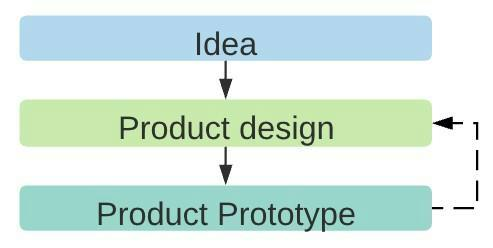
\includegraphics[width=211.7pt,height=106.49pt]{latexImage_6caaedac60a660da0197d352c225bdf8.png}}
\end{picture}
\newpage
\begin{tikzpicture}[overlay]\path(0pt,0pt);\end{tikzpicture}
\begin{picture}(-5,0)(2.5,0)
\put(500.14,-727.616){\fontsize{12}{1}\usefont{T1}{ptm}{m}{n}\selectfont\color{color_29791}43}
\put(512.14,-727.616){\fontsize{12}{1}\usefont{T1}{ptm}{m}{n}\selectfont\color{color_29791} }
\put(515.14,-727.616){\fontsize{12}{1}\usefont{T1}{ptm}{m}{n}\selectfont\color{color_29791} }
\put(70.104,-742.496){\fontsize{10.56}{1}\usefont{T1}{ptm}{m}{n}\selectfont\color{color_29791} }
\put(72.744,-742.496){\fontsize{12}{1}\usefont{T1}{ptm}{m}{n}\selectfont\color{color_29791} }
\put(515.74,-275.65){\fontsize{12}{1}\usefont{T1}{ptm}{m}{n}\selectfont\color{color_29791} }
\put(518.74,-275.65){\fontsize{12}{1}\usefont{T1}{ptm}{m}{n}\selectfont\color{color_29791} }
\put(236.93,-288.13){\fontsize{12}{1}\usefont{T1}{ptm}{m}{n}\selectfont\color{color_29791}圖}
\put(249.05,-288.13){\fontsize{12}{1}\usefont{T1}{ptm}{b}{n}\selectfont\color{color_29791}37}
\put(260.93,-288.13){\fontsize{12}{1}\usefont{T1}{ptm}{m}{n}\selectfont\color{color_29791}原型產}
\put(297.038,-288.13){\fontsize{12}{1}\usefont{T1}{ptm}{m}{n}\selectfont\color{color_29791}品專案圖}
\put(345.19,-288.13){\fontsize{12}{1}\usefont{T1}{ptm}{b}{n}\selectfont\color{color_29791} }
\put(348.07,-288.13){\fontsize{12}{1}\usefont{T1}{ptm}{m}{n}\selectfont\color{color_29791} }
\put(70.104,-305.41){\fontsize{12}{1}\usefont{T1}{ptm}{m}{n}\selectfont\color{color_29791} }
\put(73.104,-305.41){\fontsize{12}{1}\usefont{T1}{ptm}{m}{n}\selectfont\color{color_29791} }
\put(82.944,-320.53){\fontsize{12}{1}\usefont{T1}{ptm}{m}{n}\selectfont\color{color_29791}正如我們之前在第}
\put(178.94,-320.53){\fontsize{12}{1}\usefont{T1}{ptm}{m}{n}\selectfont\color{color_29791} }
\put(184.61,-320.53){\fontsize{12}{1}\usefont{T1}{ptm}{m}{n}\selectfont\color{color_29791}3 }
\put(196.37,-320.53){\fontsize{12}{1}\usefont{T1}{ptm}{m}{n}\selectfont\color{color_29791}章中所確定的}
\put(268.37,-320.53){\fontsize{12}{1}\usefont{T1}{ptm}{m}{n}\selectfont\color{color_29791},}
\put(280.37,-320.53){\fontsize{12}{1}\usefont{T1}{ptm}{m}{n}\selectfont\color{color_29791}該產品將包括}
\put(352.39,-320.53){\fontsize{12}{1}\usefont{T1}{ptm}{m}{n}\selectfont\color{color_29791} }
\put(358.03,-320.53){\fontsize{12}{1}\usefont{T1}{ptm}{m}{n}\selectfont\color{color_29791}A }
\put(371.59,-320.53){\fontsize{12}{1}\usefont{T1}{ptm}{m}{n}\selectfont\color{color_29791}部分}
\put(395.59,-320.53){\fontsize{12}{1}\usefont{T1}{ptm}{m}{n}\selectfont\color{color_29791}、}
\put(407.71,-320.53){\fontsize{12}{1}\usefont{T1}{ptm}{m}{n}\selectfont\color{color_29791}B }
\put(421.27,-320.53){\fontsize{12}{1}\usefont{T1}{ptm}{m}{n}\selectfont\color{color_29791}部}
\put(433.378,-320.53){\fontsize{12}{1}\usefont{T1}{ptm}{m}{n}\selectfont\color{color_29791}分和}
\put(457.42,-320.53){\fontsize{12}{1}\usefont{T1}{ptm}{m}{n}\selectfont\color{color_29791} }
\put(463.06,-320.53){\fontsize{12}{1}\usefont{T1}{ptm}{m}{n}\selectfont\color{color_29791}C }
\put(476.74,-320.53){\fontsize{12}{1}\usefont{T1}{ptm}{m}{n}\selectfont\color{color_29791}部分}
\put(500.74,-320.53){\fontsize{12}{1}\usefont{T1}{ptm}{m}{n}\selectfont\color{color_29791} }
\put(506.38,-320.53){\fontsize{12}{1}\usefont{T1}{ptm}{m}{n}\selectfont\color{color_29791}3 }
\put(69.384,-338.17){\fontsize{12}{1}\usefont{T1}{ptm}{m}{n}\selectfont\color{color_29791}部分}
\put(93.38,-338.17){\fontsize{12}{1}\usefont{T1}{ptm}{m}{n}\selectfont\color{color_29791}。}
\put(105.38,-338.17){\fontsize{12}{1}\usefont{T1}{ptm}{m}{n}\selectfont\color{color_29791}這些也需要作為產品進行原型設計和創建}
\put(321.43,-338.17){\fontsize{12}{1}\usefont{T1}{ptm}{m}{n}\selectfont\color{color_29791},}
\put(333.43,-338.17){\fontsize{12}{1}\usefont{T1}{ptm}{m}{n}\selectfont\color{color_29791}以便將它們添加到}
\put(429.43,-338.17){\fontsize{12}{1}\usefont{T1}{ptm}{m}{n}\selectfont\color{color_29791}P}
\put(436.138,-338.17){\fontsize{12}{1}\usefont{T1}{ptm}{m}{n}\selectfont\color{color_29791}R}
\put(444.166,-338.17){\fontsize{12}{1}\usefont{T1}{ptm}{m}{n}\selectfont\color{color_29791}OT}
\put(459.886,-338.17){\fontsize{12}{1}\usefont{T1}{ptm}{m}{n}\selectfont\color{color_29791}O }
\put(483.154,-338.17){\fontsize{12}{1}\usefont{T1}{ptm}{m}{n}\selectfont\color{color_29791}Alpha}
\put(512.434,-338.17){\fontsize{12}{1}\usefont{T1}{ptm}{m}{n}\selectfont\color{color_29791} }
\put(69.384,-355.81){\fontsize{12}{1}\usefont{T1}{ptm}{m}{n}\selectfont\color{color_29791}C}
\put(77.412,-355.81){\fontsize{12}{1}\usefont{T1}{ptm}{m}{n}\selectfont\color{color_29791}a}
\put(82.692,-355.81){\fontsize{12}{1}\usefont{T1}{ptm}{m}{n}\selectfont\color{color_29791}se}
\put(92.66,-355.81){\fontsize{12}{1}\usefont{T1}{ptm}{m}{n}\selectfont\color{color_29791}的物料清單中}
\put(164.66,-355.81){\fontsize{12}{1}\usefont{T1}{ptm}{m}{n}\selectfont\color{color_29791}。}
\put(176.66,-355.81){\fontsize{12}{1}\usefont{T1}{ptm}{m}{n}\selectfont\color{color_29791}最後}
\put(200.69,-355.81){\fontsize{12}{1}\usefont{T1}{ptm}{m}{n}\selectfont\color{color_29791},}
\put(212.69,-355.81){\fontsize{12}{1}\usefont{T1}{ptm}{m}{n}\selectfont\color{color_29791}決定使用特定的塑料長絲}
\put(344.71,-355.81){\fontsize{12}{1}\usefont{T1}{ptm}{m}{n}\selectfont\color{color_29791}(}
\put(356.71,-355.81){\fontsize{12}{1}\usefont{T1}{ptm}{m}{n}\selectfont\color{color_29791}參見第}
\put(392.71,-355.81){\fontsize{12}{1}\usefont{T1}{ptm}{m}{n}\selectfont\color{color_29791} }
\put(395.59,-355.81){\fontsize{12}{1}\usefont{T1}{ptm}{m}{n}\selectfont\color{color_29791}4.1.1 }
\put(422.47,-355.81){\fontsize{12}{1}\usefont{T1}{ptm}{m}{n}\selectfont\color{color_29791}節}
\put(434.47,-355.81){\fontsize{12}{1}\usefont{T1}{ptm}{m}{n}\selectfont\color{color_29791})}
\put(446.5,-355.81){\fontsize{12}{1}\usefont{T1}{ptm}{m}{n}\selectfont\color{color_29791}進行}
\put(470.5,-355.81){\fontsize{12}{1}\usefont{T1}{ptm}{m}{n}\selectfont\color{color_29791} }
\put(473.38,-355.81){\fontsize{12}{1}\usefont{T1}{ptm}{m}{n}\selectfont\color{color_29791}P}
\put(480.088,-355.81){\fontsize{12}{1}\usefont{T1}{ptm}{m}{n}\selectfont\color{color_29791}R}
\put(488.116,-355.81){\fontsize{12}{1}\usefont{T1}{ptm}{m}{n}\selectfont\color{color_29791}OT}
\put(503.836,-355.81){\fontsize{12}{1}\usefont{T1}{ptm}{m}{n}\selectfont\color{color_29791}O }
\put(69.384,-373.57){\fontsize{12}{1}\usefont{T1}{ptm}{m}{n}\selectfont\color{color_29791}A }
\put(80.304,-373.57){\fontsize{12}{1}\usefont{T1}{ptm}{m}{n}\selectfont\color{color_29791}部分和}
\put(116.3,-373.57){\fontsize{12}{1}\usefont{T1}{ptm}{m}{n}\selectfont\color{color_29791} }
\put(119.3,-373.57){\fontsize{12}{1}\usefont{T1}{ptm}{m}{n}\selectfont\color{color_29791}P}
\put(126.008,-373.57){\fontsize{12}{1}\usefont{T1}{ptm}{m}{n}\selectfont\color{color_29791}R}
\put(134.036,-373.57){\fontsize{12}{1}\usefont{T1}{ptm}{m}{n}\selectfont\color{color_29791}OT}
\put(149.756,-373.57){\fontsize{12}{1}\usefont{T1}{ptm}{m}{n}\selectfont\color{color_29791}O B}
\put(169.316,-373.57){\fontsize{12}{1}\usefont{T1}{ptm}{m}{n}\selectfont\color{color_29791} }
\put(172.34,-373.57){\fontsize{12}{1}\usefont{T1}{ptm}{m}{n}\selectfont\color{color_29791}部}
\put(184.448,-373.57){\fontsize{12}{1}\usefont{T1}{ptm}{m}{n}\selectfont\color{color_29791}分和}
\put(208.49,-373.57){\fontsize{12}{1}\usefont{T1}{ptm}{m}{n}\selectfont\color{color_29791} }
\put(211.49,-373.57){\fontsize{12}{1}\usefont{T1}{ptm}{m}{n}\selectfont\color{color_29791}C }
\put(222.53,-373.57){\fontsize{12}{1}\usefont{T1}{ptm}{m}{n}\selectfont\color{color_29791}部分的}
\put(258.53,-373.57){\fontsize{12}{1}\usefont{T1}{ptm}{m}{n}\selectfont\color{color_29791} }
\put(261.53,-373.57){\fontsize{12}{1}\usefont{T1}{ptm}{m}{n}\selectfont\color{color_29791}3D }
\put(279.17,-373.57){\fontsize{12}{1}\usefont{T1}{ptm}{m}{n}\selectfont\color{color_29791}列印}
\put(303.17,-373.57){\fontsize{12}{1}\usefont{T1}{ptm}{m}{n}\selectfont\color{color_29791},}
\put(315.19,-373.57){\fontsize{12}{1}\usefont{T1}{ptm}{m}{n}\selectfont\color{color_29791}這些也需要作為產品添加}
\put(447.22,-373.57){\fontsize{12}{1}\usefont{T1}{ptm}{m}{n}\selectfont\color{color_29791}(}
\put(459.22,-373.57){\fontsize{12}{1}\usefont{T1}{ptm}{m}{n}\selectfont\color{color_29791}圖}
\put(471.22,-373.57){\fontsize{12}{1}\usefont{T1}{ptm}{m}{n}\selectfont\color{color_29791} }
\put(474.22,-373.57){\fontsize{12}{1}\usefont{T1}{ptm}{m}{n}\selectfont\color{color_29791}38}
\put(486.22,-373.57){\fontsize{12}{1}\usefont{T1}{ptm}{m}{n}\selectfont\color{color_29791})。}
\put(510.22,-373.57){\fontsize{12}{1}\usefont{T1}{ptm}{m}{n}\selectfont\color{color_29791} }
\put(513.22,-373.57){\fontsize{12}{1}\usefont{T1}{ptm}{m}{n}\selectfont\color{color_29791} }
\put(70.104,-391.09){\fontsize{12}{1}\usefont{T1}{ptm}{m}{n}\selectfont\color{color_29791} }
\put(73.104,-391.09){\fontsize{12}{1}\usefont{T1}{ptm}{m}{n}\selectfont\color{color_29791} }
\put(515.74,-541.59){\fontsize{12}{1}\usefont{T1}{ptm}{m}{n}\selectfont\color{color_29791} }
\put(518.74,-541.59){\fontsize{12}{1}\usefont{T1}{ptm}{m}{n}\selectfont\color{color_29791} }
\put(215.81,-553.95){\fontsize{12}{1}\usefont{T1}{ptm}{m}{n}\selectfont\color{color_29791}圖}
\put(227.93,-553.95){\fontsize{12}{1}\usefont{T1}{ptm}{b}{n}\selectfont\color{color_29791} }
\put(230.93,-553.95){\fontsize{12}{1}\usefont{T1}{ptm}{b}{n}\selectfont\color{color_29791}38 }
\put(245.81,-553.95){\fontsize{12}{1}\usefont{T1}{ptm}{m}{n}\selectfont\color{color_29791}原型的}
\put(281.918,-553.95){\fontsize{12}{1}\usefont{T1}{ptm}{m}{n}\selectfont\color{color_29791}產品類專案概述}
\put(366.07,-553.95){\fontsize{12}{1}\usefont{T1}{ptm}{b}{n}\selectfont\color{color_29791} }
\put(368.95,-553.95){\fontsize{12}{1}\usefont{T1}{ptm}{m}{n}\selectfont\color{color_29791} }
\put(70.104,-571.35){\fontsize{12}{1}\usefont{T1}{ptm}{m}{n}\selectfont\color{color_29791} }
\put(73.104,-571.35){\fontsize{12}{1}\usefont{T1}{ptm}{m}{n}\selectfont\color{color_29791} }
\put(82.944,-586.47){\fontsize{12}{1}\usefont{T1}{ptm}{m}{n}\selectfont\color{color_29791}至此}
\put(106.94,-586.47){\fontsize{12}{1}\usefont{T1}{ptm}{m}{n}\selectfont\color{color_29791},}
\put(118.94,-586.47){\fontsize{12}{1}\usefont{T1}{ptm}{m}{n}\selectfont\color{color_29791}Alpha}
\put(148.22,-586.47){\fontsize{12}{1}\usefont{T1}{ptm}{m}{n}\selectfont\color{color_29791} }
\put(69.384,-604.14){\fontsize{12}{1}\usefont{T1}{ptm}{m}{n}\selectfont\color{color_29791}C}
\put(77.412,-604.14){\fontsize{12}{1}\usefont{T1}{ptm}{m}{n}\selectfont\color{color_29791}a}
\put(82.692,-604.14){\fontsize{12}{1}\usefont{T1}{ptm}{m}{n}\selectfont\color{color_29791}se}
\put(92.66,-604.14){\fontsize{12}{1}\usefont{T1}{ptm}{m}{n}\selectfont\color{color_29791}原型製作的相關產品專案已經完成}
\put(272.69,-604.14){\fontsize{12}{1}\usefont{T1}{ptm}{m}{n}\selectfont\color{color_29791},}
\put(284.69,-604.14){\fontsize{12}{1}\usefont{T1}{ptm}{m}{n}\selectfont\color{color_29791}這使得創建其相關}
\put(380.71,-604.14){\fontsize{12}{1}\usefont{T1}{ptm}{m}{n}\selectfont\color{color_29791}B}
\put(388.63,-604.14){\fontsize{12}{1}\usefont{T1}{ptm}{m}{n}\selectfont\color{color_29791}OM}
\put(407.95,-604.14){\fontsize{12}{1}\usefont{T1}{ptm}{m}{n}\selectfont\color{color_29791}成}
\put(420.058,-604.14){\fontsize{12}{1}\usefont{T1}{ptm}{m}{n}\selectfont\color{color_29791}為可能}
\put(456.1,-604.14){\fontsize{12}{1}\usefont{T1}{ptm}{m}{n}\selectfont\color{color_29791}。}
\put(468.1,-604.14){\fontsize{12}{1}\usefont{T1}{ptm}{m}{n}\selectfont\color{color_29791}其中有}
\put(504.1,-604.14){\fontsize{12}{1}\usefont{T1}{ptm}{m}{n}\selectfont\color{color_29791} }
\put(506.5,-604.14){\fontsize{12}{1}\usefont{T1}{ptm}{m}{n}\selectfont\color{color_29791}3 }
\put(69.384,-621.78){\fontsize{12}{1}\usefont{T1}{ptm}{m}{n}\selectfont\color{color_29791}個}
\put(81.384,-621.78){\fontsize{12}{1}\usefont{T1}{ptm}{m}{n}\selectfont\color{color_29791},}
\put(93.38,-621.78){\fontsize{12}{1}\usefont{T1}{ptm}{m}{n}\selectfont\color{color_29791}它們遵循}
\put(141.38,-621.78){\fontsize{12}{1}\usefont{T1}{ptm}{m}{n}\selectfont\color{color_29791}(}
\put(153.38,-621.78){\fontsize{12}{1}\usefont{T1}{ptm}{m}{n}\selectfont\color{color_29791}圖}
\put(165.38,-621.78){\fontsize{12}{1}\usefont{T1}{ptm}{m}{n}\selectfont\color{color_29791} }
\put(168.38,-621.78){\fontsize{12}{1}\usefont{T1}{ptm}{m}{n}\selectfont\color{color_29791}39}
\put(180.41,-621.78){\fontsize{12}{1}\usefont{T1}{ptm}{m}{n}\selectfont\color{color_29791})}
\put(192.41,-621.78){\fontsize{12}{1}\usefont{T1}{ptm}{m}{n}\selectfont\color{color_29791}中的結構}
\put(240.41,-621.78){\fontsize{12}{1}\usefont{T1}{ptm}{m}{n}\selectfont\color{color_29791}:}
\put(252.41,-621.78){\fontsize{12}{1}\usefont{T1}{ptm}{m}{n}\selectfont\color{color_29791} }
\put(255.41,-621.78){\fontsize{12}{1}\usefont{T1}{ptm}{m}{n}\selectfont\color{color_29791} }
\put(73.75,-275.6){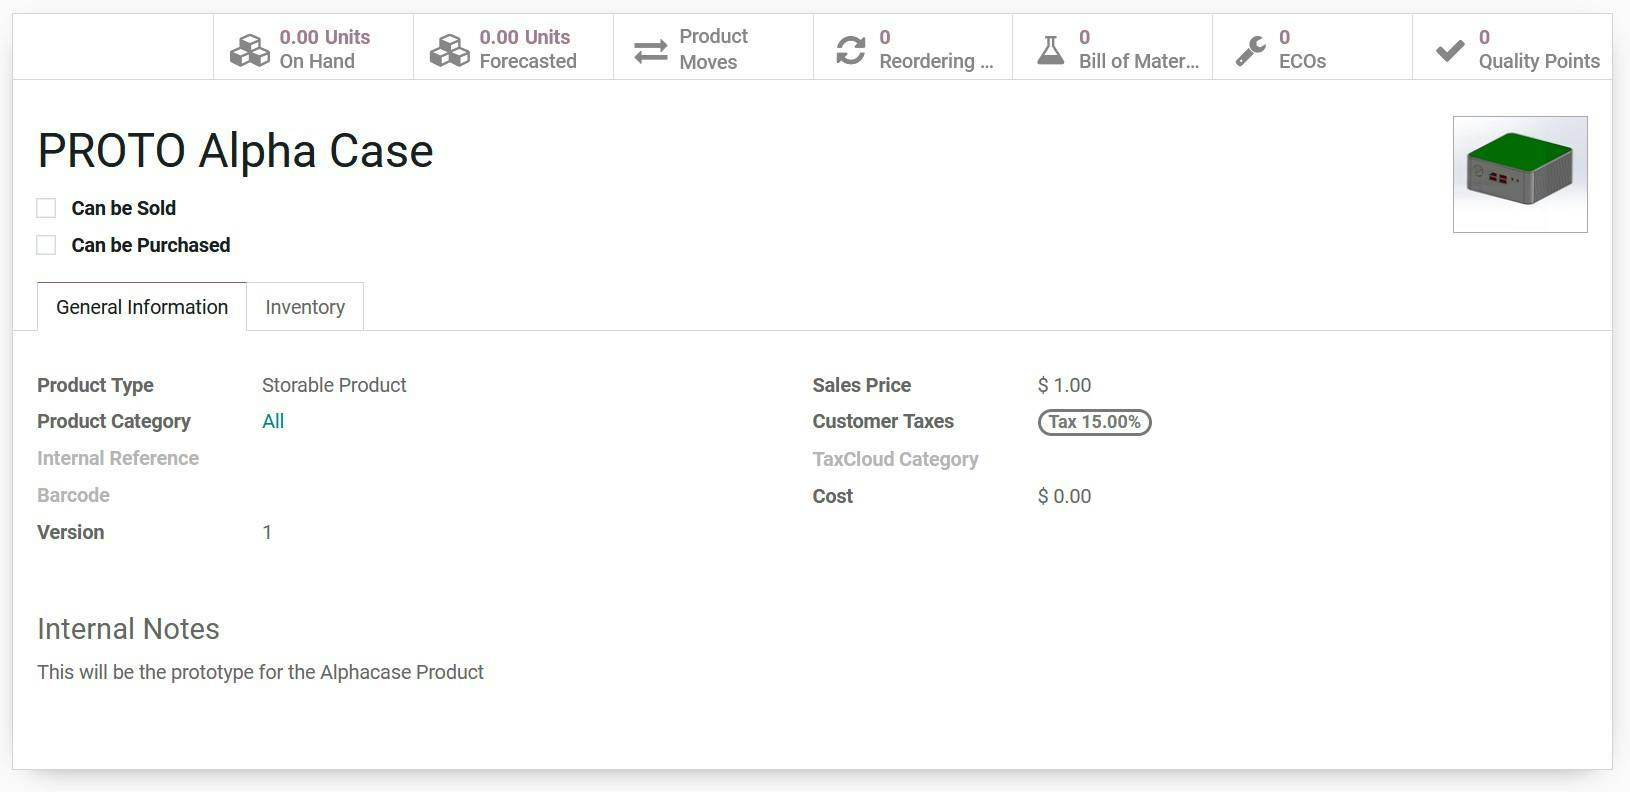
\includegraphics[width=441.9pt,height=214.7pt]{latexImage_46a08e6d8542959e1bfbe7cbd08ea400.png}}
\put(73.75,-541.43){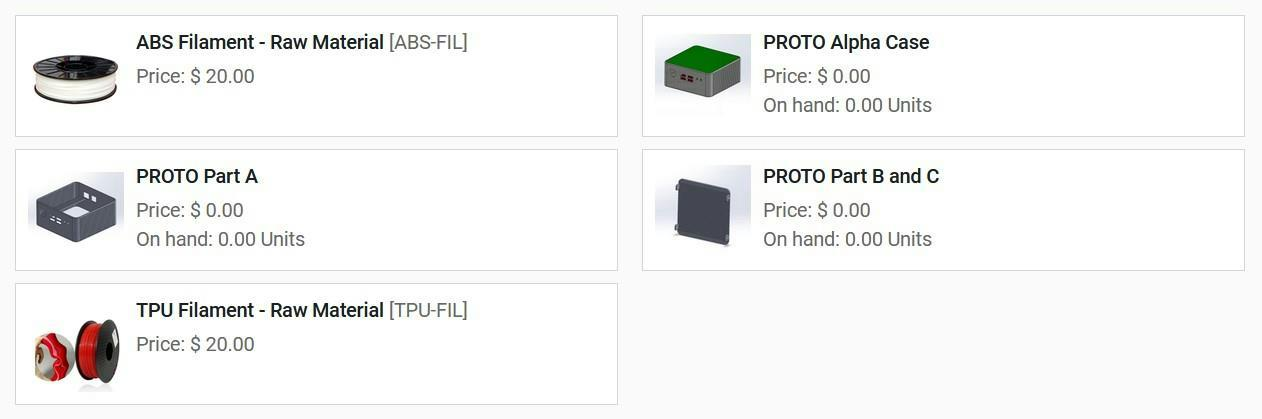
\includegraphics[width=441.9pt,height=146.7pt]{latexImage_efc1f9455a1f08e4ad0a7d56bb814dea.png}}
\end{picture}
\newpage
\begin{tikzpicture}[overlay]\path(0pt,0pt);\end{tikzpicture}
\begin{picture}(-5,0)(2.5,0)
\put(500.14,-727.616){\fontsize{12}{1}\usefont{T1}{ptm}{m}{n}\selectfont\color{color_29791}44}
\put(512.14,-727.616){\fontsize{12}{1}\usefont{T1}{ptm}{m}{n}\selectfont\color{color_29791} }
\put(515.14,-727.616){\fontsize{12}{1}\usefont{T1}{ptm}{m}{n}\selectfont\color{color_29791} }
\put(70.104,-742.496){\fontsize{10.56}{1}\usefont{T1}{ptm}{m}{n}\selectfont\color{color_29791} }
\put(72.744,-742.496){\fontsize{12}{1}\usefont{T1}{ptm}{m}{n}\selectfont\color{color_29791} }
\put(515.74,-241.78){\fontsize{12}{1}\usefont{T1}{ptm}{m}{n}\selectfont\color{color_29791} }
\put(518.74,-241.78){\fontsize{12}{1}\usefont{T1}{ptm}{m}{n}\selectfont\color{color_29791} }
\put(222.53,-254.29){\fontsize{12}{1}\usefont{T1}{ptm}{m}{n}\selectfont\color{color_29791}圖}
\put(234.65,-254.29){\fontsize{12}{1}\usefont{T1}{ptm}{b}{n}\selectfont\color{color_29791} }
\put(237.65,-254.29){\fontsize{12}{1}\usefont{T1}{ptm}{b}{n}\selectfont\color{color_29791}39 }
\put(252.53,-254.29){\fontsize{12}{1}\usefont{T1}{ptm}{m}{n}\selectfont\color{color_29791}原型製}
\put(288.638,-254.29){\fontsize{12}{1}\usefont{T1}{ptm}{m}{n}\selectfont\color{color_29791}作的}
\put(312.79,-254.29){\fontsize{12}{1}\usefont{T1}{ptm}{b}{n}\selectfont\color{color_29791} }
\put(315.67,-254.29){\fontsize{12}{1}\usefont{T1}{ptm}{b}{n}\selectfont\color{color_29791}B}
\put(323.698,-254.29){\fontsize{12}{1}\usefont{T1}{ptm}{b}{n}\selectfont\color{color_29791}OM }
\put(347.35,-254.29){\fontsize{12}{1}\usefont{T1}{ptm}{m}{n}\selectfont\color{color_29791}圖}
\put(359.47,-254.29){\fontsize{12}{1}\usefont{T1}{ptm}{b}{n}\selectfont\color{color_29791} }
\put(362.35,-254.29){\fontsize{12}{1}\usefont{T1}{ptm}{m}{n}\selectfont\color{color_29791} }
\put(70.104,-271.57){\fontsize{12}{1}\usefont{T1}{ptm}{m}{n}\selectfont\color{color_29791} }
\put(73.104,-271.57){\fontsize{12}{1}\usefont{T1}{ptm}{m}{n}\selectfont\color{color_29791} }
\put(82.944,-286.69){\fontsize{12}{1}\usefont{T1}{ptm}{m}{n}\selectfont\color{color_29791}值得一提的是}
\put(154.94,-286.69){\fontsize{12}{1}\usefont{T1}{ptm}{m}{n}\selectfont\color{color_29791},}
\put(166.94,-286.69){\fontsize{12}{1}\usefont{T1}{ptm}{m}{n}\selectfont\color{color_29791}Odoo}
\put(193.61,-286.69){\fontsize{12}{1}\usefont{T1}{ptm}{m}{n}\selectfont\color{color_29791}在專案上使用了套件選項}
\put(325.63,-286.69){\fontsize{12}{1}\usefont{T1}{ptm}{m}{n}\selectfont\color{color_29791}(}
\put(337.63,-286.69){\fontsize{12}{1}\usefont{T1}{ptm}{m}{n}\selectfont\color{color_29791}圖}
\put(349.63,-286.69){\fontsize{12}{1}\usefont{T1}{ptm}{m}{n}\selectfont\color{color_29791}40}
\put(361.63,-286.69){\fontsize{12}{1}\usefont{T1}{ptm}{m}{n}\selectfont\color{color_29791})}
\put(373.63,-286.69){\fontsize{12}{1}\usefont{T1}{ptm}{m}{n}\selectfont\color{color_29791}來推斷該產品是另一個產}
\put(69.384,-304.45){\fontsize{12}{1}\usefont{T1}{ptm}{m}{n}\selectfont\color{color_29791}品的元件}
\put(117.38,-304.45){\fontsize{12}{1}\usefont{T1}{ptm}{m}{n}\selectfont\color{color_29791}。}
\put(129.38,-304.45){\fontsize{12}{1}\usefont{T1}{ptm}{m}{n}\selectfont\color{color_29791}這非常有趣}
\put(189.41,-304.45){\fontsize{12}{1}\usefont{T1}{ptm}{m}{n}\selectfont\color{color_29791},}
\put(201.41,-304.45){\fontsize{12}{1}\usefont{T1}{ptm}{m}{n}\selectfont\color{color_29791}因為它會自動在生產產品項之間創建依賴關係}
\put(441.43,-304.45){\fontsize{12}{1}\usefont{T1}{ptm}{m}{n}\selectfont\color{color_29791}。}
\put(453.46,-304.45){\fontsize{12}{1}\usefont{T1}{ptm}{m}{n}\selectfont\color{color_29791}  }
\put(459.46,-304.45){\fontsize{12}{1}\usefont{T1}{ptm}{m}{n}\selectfont\color{color_29791} }
\put(84.264,-321.97){\fontsize{12}{1}\usefont{T1}{ptm}{m}{n}\selectfont\color{color_29791} }
\put(87.26,-321.97){\fontsize{12}{1}\usefont{T1}{ptm}{m}{n}\selectfont\color{color_29791} }
\put(512.02,-658.26){\fontsize{12}{1}\usefont{T1}{ptm}{m}{n}\selectfont\color{color_29791} }
\put(193.13,-674.34){\fontsize{12}{1}\usefont{T1}{ptm}{m}{n}\selectfont\color{color_29791}圖}
\put(205.25,-674.34){\fontsize{12}{1}\usefont{T1}{ptm}{b}{n}\selectfont\color{color_29791} }
\put(208.25,-674.34){\fontsize{12}{1}\usefont{T1}{ptm}{b}{n}\selectfont\color{color_29791}40 }
\put(223.13,-674.34){\fontsize{12}{1}\usefont{T1}{ptm}{m}{n}\selectfont\color{color_29791}原型產}
\put(259.238,-674.34){\fontsize{12}{1}\usefont{T1}{ptm}{m}{n}\selectfont\color{color_29791}品}
\put(271.37,-674.34){\fontsize{12}{1}\usefont{T1}{ptm}{b}{n}\selectfont\color{color_29791} }
\put(274.25,-674.34){\fontsize{12}{1}\usefont{T1}{ptm}{b}{n}\selectfont\color{color_29791}B}
\put(282.278,-674.34){\fontsize{12}{1}\usefont{T1}{ptm}{b}{n}\selectfont\color{color_29791}OM }
\put(305.81,-674.34){\fontsize{12}{1}\usefont{T1}{ptm}{m}{n}\selectfont\color{color_29791}影像}
\put(329.83,-674.34){\fontsize{12}{1}\usefont{T1}{ptm}{m}{n}\selectfont\color{color_29791}(}
\put(341.95,-674.34){\fontsize{12}{1}\usefont{T1}{ptm}{b}{n}\selectfont\color{color_29791}A }
\put(352.87,-674.34){\fontsize{12}{1}\usefont{T1}{ptm}{m}{n}\selectfont\color{color_29791}部分}
\put(376.87,-674.34){\fontsize{12}{1}\usefont{T1}{ptm}{m}{n}\selectfont\color{color_29791})}
\put(388.99,-674.34){\fontsize{12}{1}\usefont{T1}{ptm}{b}{n}\selectfont\color{color_29791} }
\put(391.87,-674.34){\fontsize{12}{1}\usefont{T1}{ptm}{m}{n}\selectfont\color{color_29791} }
\put(70.104,-691.616){\fontsize{12}{1}\usefont{T1}{ptm}{m}{n}\selectfont\color{color_29791} }
\put(73.104,-691.616){\fontsize{12}{1}\usefont{T1}{ptm}{m}{n}\selectfont\color{color_29791} }
\put(73.75,-241.75){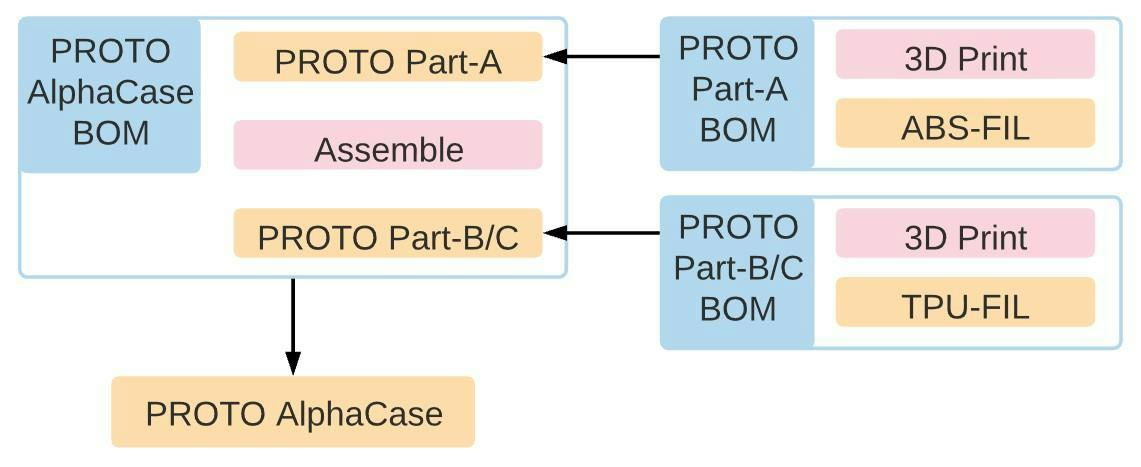
\includegraphics[width=441.9pt,height=180.85pt]{latexImage_1786e7e1d61c6c53f16eb6df9f65723a.png}}
\put(70.05,-529.13){\includegraphics[width=441.9pt,height=203.5pt]{latexImage_29a76fceb66f134f8ec25322f379ca70.png}}
\put(70.05,-658.13){\includegraphics[width=441.9pt,height=128.5pt]{latexImage_ea9f78931c89f5faa69608b830bc49c7.png}}
\end{picture}
\newpage
\begin{tikzpicture}[overlay]\path(0pt,0pt);\end{tikzpicture}
\begin{picture}(-5,0)(2.5,0)
\put(500.14,-727.616){\fontsize{12}{1}\usefont{T1}{ptm}{m}{n}\selectfont\color{color_29791}45}
\put(512.14,-727.616){\fontsize{12}{1}\usefont{T1}{ptm}{m}{n}\selectfont\color{color_29791} }
\put(515.14,-727.616){\fontsize{12}{1}\usefont{T1}{ptm}{m}{n}\selectfont\color{color_29791} }
\put(70.104,-742.496){\fontsize{10.56}{1}\usefont{T1}{ptm}{m}{n}\selectfont\color{color_29791} }
\put(72.744,-742.496){\fontsize{12}{1}\usefont{T1}{ptm}{m}{n}\selectfont\color{color_29791} }
\put(82.944,-72.34003){\fontsize{12}{1}\usefont{T1}{ptm}{m}{n}\selectfont\color{color_29791} }
\put(85.94,-72.34003){\fontsize{12}{1}\usefont{T1}{ptm}{m}{n}\selectfont\color{color_29791}正如讀者所看到的}
\put(181.97,-72.34003){\fontsize{12}{1}\usefont{T1}{ptm}{m}{n}\selectfont\color{color_29791}(}
\put(193.97,-72.34003){\fontsize{12}{1}\usefont{T1}{ptm}{m}{n}\selectfont\color{color_29791}圖}
\put(205.97,-72.34003){\fontsize{12}{1}\usefont{T1}{ptm}{m}{n}\selectfont\color{color_29791} }
\put(309.53,-72.34003){\fontsize{12}{1}\usefont{T1}{ptm}{m}{n}\selectfont\color{color_29791}41}
\put(321.55,-72.34003){\fontsize{12}{1}\usefont{T1}{ptm}{m}{n}\selectfont\color{color_29791}),}
\put(345.55,-72.34003){\fontsize{12}{1}\usefont{T1}{ptm}{m}{n}\selectfont\color{color_29791}在製作}
\put(381.55,-72.34003){\fontsize{12}{1}\usefont{T1}{ptm}{m}{n}\selectfont\color{color_29791} }
\put(485.14,-72.34003){\fontsize{12}{1}\usefont{T1}{ptm}{m}{n}\selectfont\color{color_29791}B}
\put(493.06,-72.34003){\fontsize{12}{1}\usefont{T1}{ptm}{m}{n}\selectfont\color{color_29791}O}
\put(501.808,-72.34003){\fontsize{12}{1}\usefont{T1}{ptm}{m}{n}\selectfont\color{color_29791}M }
\put(69.384,-89.97998){\fontsize{12}{1}\usefont{T1}{ptm}{m}{n}\selectfont\color{color_29791}時}
\put(81.384,-89.97998){\fontsize{12}{1}\usefont{T1}{ptm}{m}{n}\selectfont\color{color_29791},}
\put(93.38,-89.97998){\fontsize{12}{1}\usefont{T1}{ptm}{m}{n}\selectfont\color{color_29791}創建製造過程所需的特定操作專案並指定其工作中心非常簡單}
\put(417.43,-89.97998){\fontsize{12}{1}\usefont{T1}{ptm}{m}{n}\selectfont\color{color_29791}。}
\put(429.43,-89.97998){\fontsize{12}{1}\usefont{T1}{ptm}{m}{n}\selectfont\color{color_29791}Odoo}
\put(456.1,-89.97998){\fontsize{12}{1}\usefont{T1}{ptm}{m}{n}\selectfont\color{color_29791}中}
\put(468.1,-89.97998){\fontsize{12}{1}\usefont{T1}{ptm}{m}{n}\selectfont\color{color_29791}M}
\put(478.78,-89.97998){\fontsize{12}{1}\usefont{T1}{ptm}{m}{n}\selectfont\color{color_29791}ES}
\put(492.82,-89.97998){\fontsize{12}{1}\usefont{T1}{ptm}{m}{n}\selectfont\color{color_29791}的}
\put(69.384,-107.62){\fontsize{12}{1}\usefont{T1}{ptm}{m}{n}\selectfont\color{color_29791}最佳功能之一是能夠根據預設持續時間跟蹤操作時間}
\put(345.43,-107.62){\fontsize{12}{1}\usefont{T1}{ptm}{m}{n}\selectfont\color{color_29791}。}
\put(357.43,-107.62){\fontsize{12}{1}\usefont{T1}{ptm}{m}{n}\selectfont\color{color_29791}這可以根據跟蹤時間動態更}
\put(69.384,-125.14){\fontsize{12}{1}\usefont{T1}{ptm}{m}{n}\selectfont\color{color_29791}改或手動設置}
\put(141.38,-125.14){\fontsize{12}{1}\usefont{T1}{ptm}{m}{n}\selectfont\color{color_29791}。}
\put(153.38,-125.14){\fontsize{12}{1}\usefont{T1}{ptm}{m}{n}\selectfont\color{color_29791} }
\put(69.384,-142.78){\fontsize{12}{1}\usefont{T1}{ptm}{m}{n}\selectfont\color{color_29791}同樣在操作項中}
\put(153.38,-142.78){\fontsize{12}{1}\usefont{T1}{ptm}{m}{n}\selectfont\color{color_29791},}
\put(165.38,-142.78){\fontsize{12}{1}\usefont{T1}{ptm}{m}{n}\selectfont\color{color_29791}我們可以為操作添加指令檔}
\put(309.41,-142.78){\fontsize{12}{1}\usefont{T1}{ptm}{m}{n}\selectfont\color{color_29791}。}
\put(321.43,-142.78){\fontsize{12}{1}\usefont{T1}{ptm}{m}{n}\selectfont\color{color_29791}儘管它僅限於}
\put(393.43,-142.78){\fontsize{12}{1}\usefont{T1}{ptm}{m}{n}\selectfont\color{color_29791}P}
\put(400.138,-142.78){\fontsize{12}{1}\usefont{T1}{ptm}{m}{n}\selectfont\color{color_29791}DF}
\put(415.39,-142.78){\fontsize{12}{1}\usefont{T1}{ptm}{m}{n}\selectfont\color{color_29791}文}
\put(427.498,-142.78){\fontsize{12}{1}\usefont{T1}{ptm}{m}{n}\selectfont\color{color_29791}本或指向谷歌幻}
\put(69.384,-160.54){\fontsize{12}{1}\usefont{T1}{ptm}{m}{n}\selectfont\color{color_29791}燈片文件的連結}
\put(154.22,-160.54){\fontsize{12}{1}\usefont{T1}{ptm}{m}{n}\selectfont\color{color_29791},}
\put(166.34,-160.54){\fontsize{12}{1}\usefont{T1}{ptm}{m}{n}\selectfont\color{color_29791}但這是}
\put(203.09,-160.54){\fontsize{12}{1}\usefont{T1}{ptm}{m}{n}\selectfont\color{color_29791}O}
\put(211.958,-160.54){\fontsize{12}{1}\usefont{T1}{ptm}{m}{n}\selectfont\color{color_29791}d}
\put(218.186,-160.54){\fontsize{12}{1}\usefont{T1}{ptm}{m}{n}\selectfont\color{color_29791}o}
\put(224.414,-160.54){\fontsize{12}{1}\usefont{T1}{ptm}{m}{n}\selectfont\color{color_29791}o}
\put(230.69,-160.54){\fontsize{12}{1}\usefont{T1}{ptm}{m}{n}\selectfont\color{color_29791}提供的為數不多的直接連接到專案的檔管理機會之一}
\put(512.26,-160.54){\fontsize{12}{1}\usefont{T1}{ptm}{m}{n}\selectfont\color{color_29791}。}
\put(524.5,-160.54){\fontsize{12}{1}\usefont{T1}{ptm}{m}{n}\selectfont\color{color_29791} }
\put(527.5,-160.54){\fontsize{12}{1}\usefont{T1}{ptm}{m}{n}\selectfont\color{color_29791} }
\put(70.104,-178.06){\fontsize{12}{1}\usefont{T1}{ptm}{m}{n}\selectfont\color{color_29791} }
\put(73.104,-178.06){\fontsize{12}{1}\usefont{T1}{ptm}{m}{n}\selectfont\color{color_29791} }
\put(515.74,-514.23){\fontsize{12}{1}\usefont{T1}{ptm}{m}{n}\selectfont\color{color_29791} }
\put(518.74,-514.23){\fontsize{12}{1}\usefont{T1}{ptm}{m}{n}\selectfont\color{color_29791} }
\put(160.82,-534.87){\fontsize{12}{1}\usefont{T1}{ptm}{m}{n}\selectfont\color{color_29791}圖}
\put(172.94,-534.87){\fontsize{12}{1}\usefont{T1}{ptm}{b}{n}\selectfont\color{color_29791} }
\put(175.94,-534.87){\fontsize{12}{1}\usefont{T1}{ptm}{b}{n}\selectfont\color{color_29791}41 }
\put(190.97,-534.87){\fontsize{12}{1}\usefont{T1}{ptm}{b}{n}\selectfont\color{color_29791}Od}
\put(207.038,-534.87){\fontsize{12}{1}\usefont{T1}{ptm}{b}{n}\selectfont\color{color_29791}oo }
\put(221.93,-534.87){\fontsize{12}{1}\usefont{T1}{ptm}{m}{n}\selectfont\color{color_29791}顯示的操作項目圖像}
\put(330.07,-534.87){\fontsize{12}{1}\usefont{T1}{ptm}{m}{n}\selectfont\color{color_29791}(}
\put(342.07,-534.87){\fontsize{12}{1}\usefont{T1}{ptm}{b}{n}\selectfont\color{color_29791}B}
\put(350.098,-534.87){\fontsize{12}{1}\usefont{T1}{ptm}{b}{n}\selectfont\color{color_29791}OM P}
\put(380.938,-534.87){\fontsize{12}{1}\usefont{T1}{ptm}{b}{n}\selectfont\color{color_29791}ar}
\put(392.218,-534.87){\fontsize{12}{1}\usefont{T1}{ptm}{b}{n}\selectfont\color{color_29791}t}
\put(396.31,-534.87){\fontsize{12}{1}\usefont{T1}{ptm}{b}{n}\selectfont\color{color_29791}-}
\put(400.39,-534.87){\fontsize{12}{1}\usefont{T1}{ptm}{b}{n}\selectfont\color{color_29791}A}
\put(409.03,-534.87){\fontsize{12}{1}\usefont{T1}{ptm}{m}{n}\selectfont\color{color_29791})}
\put(421.15,-534.87){\fontsize{12}{1}\usefont{T1}{ptm}{b}{n}\selectfont\color{color_29791} }
\put(424.03,-534.87){\fontsize{12}{1}\usefont{T1}{ptm}{m}{n}\selectfont\color{color_29791} }
\put(70.104,-552.27){\fontsize{12}{1}\usefont{T1}{ptm}{m}{n}\selectfont\color{color_29791} }
\put(73.104,-552.27){\fontsize{12}{1}\usefont{T1}{ptm}{m}{n}\selectfont\color{color_29791} }
\put(70.104,-567.15){\fontsize{12}{1}\usefont{T1}{ptm}{m}{n}\selectfont\color{color_29791} }
\put(73.104,-567.15){\fontsize{12}{1}\usefont{T1}{ptm}{m}{n}\selectfont\color{color_29791} }
\put(506.74,-698.096){\fontsize{12}{1}\usefont{T1}{ptm}{m}{n}\selectfont\color{color_29791} }
\put(509.74,-698.096){\fontsize{12}{1}\usefont{T1}{ptm}{m}{n}\selectfont\color{color_29791} }
\put(73.75,-514.1901){\includegraphics[width=441.9pt,height=332.45pt]{latexImage_a8994286f009e31acda7fefd5ee76759.png}}
\put(73.25,-697.9691){\includegraphics[width=433.4pt,height=127.2pt]{latexImage_a968e9cd824729073f0b4772388ad3e8.png}}
\end{picture}
\newpage
\begin{tikzpicture}[overlay]\path(0pt,0pt);\end{tikzpicture}
\begin{picture}(-5,0)(2.5,0)
\put(500.14,-727.616){\fontsize{12}{1}\usefont{T1}{ptm}{m}{n}\selectfont\color{color_29791}46}
\put(512.14,-727.616){\fontsize{12}{1}\usefont{T1}{ptm}{m}{n}\selectfont\color{color_29791} }
\put(515.14,-727.616){\fontsize{12}{1}\usefont{T1}{ptm}{m}{n}\selectfont\color{color_29791} }
\put(70.104,-742.496){\fontsize{10.56}{1}\usefont{T1}{ptm}{m}{n}\selectfont\color{color_29791} }
\put(72.744,-742.496){\fontsize{12}{1}\usefont{T1}{ptm}{m}{n}\selectfont\color{color_29791} }
\put(198.53,-72.34003){\fontsize{12}{1}\usefont{T1}{ptm}{m}{n}\selectfont\color{color_29791}圖}
\put(210.65,-72.34003){\fontsize{12}{1}\usefont{T1}{ptm}{b}{n}\selectfont\color{color_29791} }
\put(213.65,-72.34003){\fontsize{12}{1}\usefont{T1}{ptm}{b}{n}\selectfont\color{color_29791}42 }
\put(228.53,-72.34003){\fontsize{12}{1}\usefont{T1}{ptm}{m}{n}\selectfont\color{color_29791}為原型}
\put(264.638,-72.34003){\fontsize{12}{1}\usefont{T1}{ptm}{m}{n}\selectfont\color{color_29791}設計創建的}
\put(324.79,-72.34003){\fontsize{12}{1}\usefont{T1}{ptm}{b}{n}\selectfont\color{color_29791} }
\put(327.79,-72.34003){\fontsize{12}{1}\usefont{T1}{ptm}{b}{n}\selectfont\color{color_29791}B}
\put(335.818,-72.34003){\fontsize{12}{1}\usefont{T1}{ptm}{b}{n}\selectfont\color{color_29791}OM }
\put(359.35,-72.34003){\fontsize{12}{1}\usefont{T1}{ptm}{m}{n}\selectfont\color{color_29791}概述}
\put(383.47,-72.34003){\fontsize{12}{1}\usefont{T1}{ptm}{b}{n}\selectfont\color{color_29791} }
\put(386.35,-72.34003){\fontsize{12}{1}\usefont{T1}{ptm}{m}{n}\selectfont\color{color_29791} }
\put(70.104,-89.62){\fontsize{12}{1}\usefont{T1}{ptm}{m}{n}\selectfont\color{color_29791} }
\put(73.104,-89.62){\fontsize{12}{1}\usefont{T1}{ptm}{m}{n}\selectfont\color{color_29791} }
\put(82.944,-104.74){\fontsize{12}{1}\usefont{T1}{ptm}{m}{n}\selectfont\color{color_29791}說到這種缺乏上傳機會}
\put(202.97,-104.74){\fontsize{12}{1}\usefont{T1}{ptm}{m}{n}\selectfont\color{color_29791},}
\put(214.97,-104.74){\fontsize{12}{1}\usefont{T1}{ptm}{m}{n}\selectfont\color{color_29791}我們可以注意到}
\put(298.97,-104.74){\fontsize{12}{1}\usefont{T1}{ptm}{m}{n}\selectfont\color{color_29791},}
\put(310.97,-104.74){\fontsize{12}{1}\usefont{T1}{ptm}{m}{n}\selectfont\color{color_29791}在製作產品專案時}
\put(406.99,-104.74){\fontsize{12}{1}\usefont{T1}{ptm}{m}{n}\selectfont\color{color_29791},}
\put(418.99,-104.74){\fontsize{12}{1}\usefont{T1}{ptm}{m}{n}\selectfont\color{color_29791}無法直接將有關}
\put(69.384,-122.38){\fontsize{12}{1}\usefont{T1}{ptm}{m}{n}\selectfont\color{color_29791}產品的檔上傳到專案}
\put(177.38,-122.38){\fontsize{12}{1}\usefont{T1}{ptm}{m}{n}\selectfont\color{color_29791}。}
\put(189.41,-122.38){\fontsize{12}{1}\usefont{T1}{ptm}{m}{n}\selectfont\color{color_29791}在我們的案例中}
\put(273.41,-122.38){\fontsize{12}{1}\usefont{T1}{ptm}{m}{n}\selectfont\color{color_29791},}
\put(285.41,-122.38){\fontsize{12}{1}\usefont{T1}{ptm}{m}{n}\selectfont\color{color_29791}我們有關於我們正在原型製作的零件的}
\put(489.46,-122.38){\fontsize{12}{1}\usefont{T1}{ptm}{m}{n}\selectfont\color{color_29791} }
\put(69.384,-140.02){\fontsize{12}{1}\usefont{T1}{ptm}{m}{n}\selectfont\color{color_29791}C}
\put(77.412,-140.02){\fontsize{12}{1}\usefont{T1}{ptm}{m}{n}\selectfont\color{color_29791}AD}
\put(94.692,-140.02){\fontsize{12}{1}\usefont{T1}{ptm}{m}{n}\selectfont\color{color_29791} }
\put(273.29,-140.02){\fontsize{12}{1}\usefont{T1}{ptm}{m}{n}\selectfont\color{color_29791}檔}
\put(285.29,-140.02){\fontsize{12}{1}\usefont{T1}{ptm}{m}{n}\selectfont\color{color_29791},}
\put(297.29,-140.02){\fontsize{12}{1}\usefont{T1}{ptm}{m}{n}\selectfont\color{color_29791}從}
\put(309.29,-140.02){\fontsize{12}{1}\usefont{T1}{ptm}{m}{n}\selectfont\color{color_29791} }
\put(487.9,-140.02){\fontsize{12}{1}\usefont{T1}{ptm}{m}{n}\selectfont\color{color_29791}P}
\put(494.728,-140.02){\fontsize{12}{1}\usefont{T1}{ptm}{m}{n}\selectfont\color{color_29791}L}
\put(501.808,-140.02){\fontsize{12}{1}\usefont{T1}{ptm}{m}{n}\selectfont\color{color_29791}M }
\put(69.384,-157.66){\fontsize{12}{1}\usefont{T1}{ptm}{m}{n}\selectfont\color{color_29791}的角度來看}
\put(129.38,-157.66){\fontsize{12}{1}\usefont{T1}{ptm}{m}{n}\selectfont\color{color_29791},}
\put(141.38,-157.66){\fontsize{12}{1}\usefont{T1}{ptm}{m}{n}\selectfont\color{color_29791}無法以任何方式上傳這些檔將是一個完全失敗的過程}
\put(417.43,-157.66){\fontsize{12}{1}\usefont{T1}{ptm}{m}{n}\selectfont\color{color_29791}。}
\put(429.43,-157.66){\fontsize{12}{1}\usefont{T1}{ptm}{m}{n}\selectfont\color{color_29791}值得慶幸的是}
\put(69.384,-175.3){\fontsize{12}{1}\usefont{T1}{ptm}{m}{n}\selectfont\color{color_29791},}
\put(81.384,-175.3){\fontsize{12}{1}\usefont{T1}{ptm}{m}{n}\selectfont\color{color_29791}有一個解決方法}
\put(165.38,-175.3){\fontsize{12}{1}\usefont{T1}{ptm}{m}{n}\selectfont\color{color_29791}。}
\put(177.38,-175.3){\fontsize{12}{1}\usefont{T1}{ptm}{m}{n}\selectfont\color{color_29791}如第}
\put(201.41,-175.3){\fontsize{12}{1}\usefont{T1}{ptm}{m}{n}\selectfont\color{color_29791} }
\put(304.49,-175.3){\fontsize{12}{1}\usefont{T1}{ptm}{m}{n}\selectfont\color{color_29791}5.1.3.5 }
\put(440.59,-175.3){\fontsize{12}{1}\usefont{T1}{ptm}{m}{n}\selectfont\color{color_29791}節所述}
\put(476.62,-175.3){\fontsize{12}{1}\usefont{T1}{ptm}{m}{n}\selectfont\color{color_29791},}
\put(488.62,-175.3){\fontsize{12}{1}\usefont{T1}{ptm}{m}{n}\selectfont\color{color_29791}ECO}
\put(512.5,-175.3){\fontsize{12}{1}\usefont{T1}{ptm}{m}{n}\selectfont\color{color_29791} }
\put(69.384,-192.94){\fontsize{12}{1}\usefont{T1}{ptm}{m}{n}\selectfont\color{color_29791}是鏈接到產品物料或物料清單並允許將上傳的檔附加到其中的物料}
\put(417.43,-192.94){\fontsize{12}{1}\usefont{T1}{ptm}{m}{n}\selectfont\color{color_29791}。}
\put(429.43,-192.94){\fontsize{12}{1}\usefont{T1}{ptm}{m}{n}\selectfont\color{color_29791}這是一個次要}
\put(69.384,-210.46){\fontsize{12}{1}\usefont{T1}{ptm}{m}{n}\selectfont\color{color_29791}的解決方法}
\put(129.38,-210.46){\fontsize{12}{1}\usefont{T1}{ptm}{m}{n}\selectfont\color{color_29791},}
\put(141.38,-210.46){\fontsize{12}{1}\usefont{T1}{ptm}{m}{n}\selectfont\color{color_29791}但基本上意味著如果我們想以任何有意義的方式將}
\put(405.43,-210.46){\fontsize{12}{1}\usefont{T1}{ptm}{m}{n}\selectfont\color{color_29791} }
\put(487.18,-210.46){\fontsize{12}{1}\usefont{T1}{ptm}{m}{n}\selectfont\color{color_29791}C}
\put(495.208,-210.46){\fontsize{12}{1}\usefont{T1}{ptm}{m}{n}\selectfont\color{color_29791}AD}
\put(512.488,-210.46){\fontsize{12}{1}\usefont{T1}{ptm}{m}{n}\selectfont\color{color_29791} }
\put(69.384,-228.1){\fontsize{12}{1}\usefont{T1}{ptm}{m}{n}\selectfont\color{color_29791}檔上傳到專案}
\put(141.38,-228.1){\fontsize{12}{1}\usefont{T1}{ptm}{m}{n}\selectfont\color{color_29791},}
\put(153.38,-228.1){\fontsize{12}{1}\usefont{T1}{ptm}{m}{n}\selectfont\color{color_29791}即使沒有進行}
\put(225.41,-228.1){\fontsize{12}{1}\usefont{T1}{ptm}{m}{n}\selectfont\color{color_29791}“ }
\put(233.69,-228.1){\fontsize{12}{1}\usefont{T1}{ptm}{m}{n}\selectfont\color{color_29791}更改}
\put(257.69,-228.1){\fontsize{12}{1}\usefont{T1}{ptm}{m}{n}\selectfont\color{color_29791}” }
\put(266.09,-228.1){\fontsize{12}{1}\usefont{T1}{ptm}{m}{n}\selectfont\color{color_29791} }
\put(515.74,-472.83){\fontsize{12}{1}\usefont{T1}{ptm}{m}{n}\selectfont\color{color_29791} }
\put(518.74,-472.83){\fontsize{12}{1}\usefont{T1}{ptm}{m}{n}\selectfont\color{color_29791} }
\put(249.41,-493.35){\fontsize{12}{1}\usefont{T1}{ptm}{m}{n}\selectfont\color{color_29791}圖}
\put(261.53,-493.35){\fontsize{12}{1}\usefont{T1}{ptm}{b}{n}\selectfont\color{color_29791} }
\put(264.53,-493.35){\fontsize{12}{1}\usefont{T1}{ptm}{b}{n}\selectfont\color{color_29791}43 }
\put(279.53,-493.35){\fontsize{12}{1}\usefont{T1}{ptm}{b}{n}\selectfont\color{color_29791}E}
\put(287.558,-493.35){\fontsize{12}{1}\usefont{T1}{ptm}{b}{n}\selectfont\color{color_29791}CO }
\put(308.45,-493.35){\fontsize{12}{1}\usefont{T1}{ptm}{m}{n}\selectfont\color{color_29791}示例}
\put(332.59,-493.35){\fontsize{12}{1}\usefont{T1}{ptm}{b}{n}\selectfont\color{color_29791} }
\put(335.47,-493.35){\fontsize{12}{1}\usefont{T1}{ptm}{m}{n}\selectfont\color{color_29791} }
\put(70.104,-510.75){\fontsize{12}{1}\usefont{T1}{ptm}{m}{n}\selectfont\color{color_29791} }
\put(73.104,-510.75){\fontsize{12}{1}\usefont{T1}{ptm}{m}{n}\selectfont\color{color_29791} }
\put(82.944,-525.87){\fontsize{12}{1}\usefont{T1}{ptm}{m}{n}\selectfont\color{color_29791}只能}
\put(106.94,-525.87){\fontsize{12}{1}\usefont{T1}{ptm}{m}{n}\selectfont\color{color_29791}假設這是}
\put(154.94,-525.87){\fontsize{12}{1}\usefont{T1}{ptm}{m}{n}\selectfont\color{color_29791}Odoo}
\put(181.61,-525.87){\fontsize{12}{1}\usefont{T1}{ptm}{m}{n}\selectfont\color{color_29791}團隊戰略的一部分}
\put(277.61,-525.87){\fontsize{12}{1}\usefont{T1}{ptm}{m}{n}\selectfont\color{color_29791},}
\put(289.61,-525.87){\fontsize{12}{1}\usefont{T1}{ptm}{m}{n}\selectfont\color{color_29791}即在其}
\put(325.63,-525.87){\fontsize{12}{1}\usefont{T1}{ptm}{m}{n}\selectfont\color{color_29791}ERP}
\put(347.71,-525.87){\fontsize{12}{1}\usefont{T1}{ptm}{m}{n}\selectfont\color{color_29791}基礎中將}
\put(395.71,-525.87){\fontsize{12}{1}\usefont{T1}{ptm}{m}{n}\selectfont\color{color_29791}P}
\put(402.418,-525.87){\fontsize{12}{1}\usefont{T1}{ptm}{m}{n}\selectfont\color{color_29791}L}
\put(409.498,-525.87){\fontsize{12}{1}\usefont{T1}{ptm}{m}{n}\selectfont\color{color_29791}M}
\put(420.19,-525.87){\fontsize{12}{1}\usefont{T1}{ptm}{m}{n}\selectfont\color{color_29791}作為}
\put(444.298,-525.87){\fontsize{12}{1}\usefont{T1}{ptm}{m}{n}\selectfont\color{color_29791}外部應用程}
\put(69.384,-543.51){\fontsize{12}{1}\usefont{T1}{ptm}{m}{n}\selectfont\color{color_29791}序實施}
\put(105.38,-543.51){\fontsize{12}{1}\usefont{T1}{ptm}{m}{n}\selectfont\color{color_29791}。}
\put(117.38,-543.51){\fontsize{12}{1}\usefont{T1}{ptm}{m}{n}\selectfont\color{color_29791}這是合理的}
\put(177.38,-543.51){\fontsize{12}{1}\usefont{T1}{ptm}{m}{n}\selectfont\color{color_29791},}
\put(189.41,-543.51){\fontsize{12}{1}\usefont{T1}{ptm}{m}{n}\selectfont\color{color_29791}但這仍然是該軟體介面為數不多的不那麼簡單的方面之一}
\put(489.46,-543.51){\fontsize{12}{1}\usefont{T1}{ptm}{m}{n}\selectfont\color{color_29791}。}
\put(69.384,-561.15){\fontsize{12}{1}\usefont{T1}{ptm}{m}{n}\selectfont\color{color_29791}這是一個非常有價值的功能}
\put(213.41,-561.15){\fontsize{12}{1}\usefont{T1}{ptm}{m}{n}\selectfont\color{color_29791},}
\put(225.41,-561.15){\fontsize{12}{1}\usefont{T1}{ptm}{m}{n}\selectfont\color{color_29791}但它有些隱藏}
\put(297.41,-561.15){\fontsize{12}{1}\usefont{T1}{ptm}{m}{n}\selectfont\color{color_29791}。}
\put(309.41,-561.15){\fontsize{12}{1}\usefont{T1}{ptm}{m}{n}\selectfont\color{color_29791}文件圖示僅在創建並保存}
\put(441.43,-561.15){\fontsize{12}{1}\usefont{T1}{ptm}{m}{n}\selectfont\color{color_29791}ECO}
\put(465.46,-561.15){\fontsize{12}{1}\usefont{T1}{ptm}{m}{n}\selectfont\color{color_29791}後才會}
\put(69.384,-578.79){\fontsize{12}{1}\usefont{T1}{ptm}{m}{n}\selectfont\color{color_29791}出現在右上角}
\put(141.38,-578.79){\fontsize{12}{1}\usefont{T1}{ptm}{m}{n}\selectfont\color{color_29791}(}
\put(153.38,-578.79){\fontsize{12}{1}\usefont{T1}{ptm}{m}{n}\selectfont\color{color_29791}圖}
\put(165.38,-578.79){\fontsize{12}{1}\usefont{T1}{ptm}{m}{n}\selectfont\color{color_29791} }
\put(168.38,-578.79){\fontsize{12}{1}\usefont{T1}{ptm}{m}{n}\selectfont\color{color_29791}43}
\put(180.41,-578.79){\fontsize{12}{1}\usefont{T1}{ptm}{m}{n}\selectfont\color{color_29791})。}
\put(204.41,-578.79){\fontsize{12}{1}\usefont{T1}{ptm}{m}{n}\selectfont\color{color_29791} }
\put(207.41,-578.79){\fontsize{12}{1}\usefont{T1}{ptm}{m}{n}\selectfont\color{color_29791} }
\put(70.104,-596.34){\fontsize{12}{1}\usefont{T1}{ptm}{m}{n}\selectfont\color{color_29791} }
\put(73.104,-596.34){\fontsize{12}{1}\usefont{T1}{ptm}{m}{n}\selectfont\color{color_29791} }
\put(73.75,-472.7){\includegraphics[width=441.9pt,height=230.85pt]{latexImage_f98ffa7113051518810c74e47cdbd9a5.png}}
\end{picture}
\newpage
\begin{tikzpicture}[overlay]\path(0pt,0pt);\end{tikzpicture}
\begin{picture}(-5,0)(2.5,0)
\put(500.14,-727.616){\fontsize{12}{1}\usefont{T1}{ptm}{m}{n}\selectfont\color{color_29791}47}
\put(512.14,-727.616){\fontsize{12}{1}\usefont{T1}{ptm}{m}{n}\selectfont\color{color_29791} }
\put(515.14,-727.616){\fontsize{12}{1}\usefont{T1}{ptm}{m}{n}\selectfont\color{color_29791} }
\put(70.104,-742.496){\fontsize{10.56}{1}\usefont{T1}{ptm}{m}{n}\selectfont\color{color_29791} }
\put(72.744,-742.496){\fontsize{12}{1}\usefont{T1}{ptm}{m}{n}\selectfont\color{color_29791} }
\put(515.74,-253.33){\fontsize{12}{1}\usefont{T1}{ptm}{m}{n}\selectfont\color{color_29791} }
\put(518.74,-253.33){\fontsize{12}{1}\usefont{T1}{ptm}{m}{n}\selectfont\color{color_29791} }
\put(240.41,-265.81){\fontsize{12}{1}\usefont{T1}{ptm}{m}{n}\selectfont\color{color_29791}圖}
\put(252.53,-265.81){\fontsize{12}{1}\usefont{T1}{ptm}{b}{n}\selectfont\color{color_29791}44 }
\put(267.53,-265.81){\fontsize{12}{1}\usefont{T1}{ptm}{b}{n}\selectfont\color{color_29791}E}
\put(275.558,-265.81){\fontsize{12}{1}\usefont{T1}{ptm}{b}{n}\selectfont\color{color_29791}CO}
\put(293.45,-265.81){\fontsize{12}{1}\usefont{T1}{ptm}{m}{n}\selectfont\color{color_29791}附件概覽}
\put(341.59,-265.81){\fontsize{12}{1}\usefont{T1}{ptm}{b}{n}\selectfont\color{color_29791} }
\put(344.47,-265.81){\fontsize{12}{1}\usefont{T1}{ptm}{m}{n}\selectfont\color{color_29791} }
\put(70.104,-283.09){\fontsize{12}{1}\usefont{T1}{ptm}{m}{n}\selectfont\color{color_29791} }
\put(73.104,-283.09){\fontsize{12}{1}\usefont{T1}{ptm}{m}{n}\selectfont\color{color_29791} }
\put(82.944,-298.21){\fontsize{12}{1}\usefont{T1}{ptm}{m}{n}\selectfont\color{color_29791}由於}
\put(106.94,-298.21){\fontsize{12}{1}\usefont{T1}{ptm}{m}{n}\selectfont\color{color_29791}Odoo}
\put(133.58,-298.21){\fontsize{12}{1}\usefont{T1}{ptm}{m}{n}\selectfont\color{color_29791}和}
\put(145.58,-298.21){\fontsize{12}{1}\usefont{T1}{ptm}{m}{n}\selectfont\color{color_29791}C}
\put(153.608,-298.21){\fontsize{12}{1}\usefont{T1}{ptm}{m}{n}\selectfont\color{color_29791}AD}
\put(170.9,-298.21){\fontsize{12}{1}\usefont{T1}{ptm}{m}{n}\selectfont\color{color_29791}軟體之間沒有直接集成}
\put(290.93,-298.21){\fontsize{12}{1}\usefont{T1}{ptm}{m}{n}\selectfont\color{color_29791},}
\put(302.93,-298.21){\fontsize{12}{1}\usefont{T1}{ptm}{m}{n}\selectfont\color{color_29791}因此上傳檔不會導致產品元數據自動更}
\put(69.384,-315.85){\fontsize{12}{1}\usefont{T1}{ptm}{m}{n}\selectfont\color{color_29791}改}
\put(81.384,-315.85){\fontsize{12}{1}\usefont{T1}{ptm}{m}{n}\selectfont\color{color_29791}。}
\put(93.38,-315.85){\fontsize{12}{1}\usefont{T1}{ptm}{m}{n}\selectfont\color{color_29791}從}
\put(105.38,-315.85){\fontsize{12}{1}\usefont{T1}{ptm}{m}{n}\selectfont\color{color_29791}P}
\put(112.208,-315.85){\fontsize{12}{1}\usefont{T1}{ptm}{m}{n}\selectfont\color{color_29791}L}
\put(119.288,-315.85){\fontsize{12}{1}\usefont{T1}{ptm}{m}{n}\selectfont\color{color_29791}M}
\put(129.98,-315.85){\fontsize{12}{1}\usefont{T1}{ptm}{m}{n}\selectfont\color{color_29791}的角度來看}
\put(190.13,-315.85){\fontsize{12}{1}\usefont{T1}{ptm}{m}{n}\selectfont\color{color_29791},}
\put(202.13,-315.85){\fontsize{12}{1}\usefont{T1}{ptm}{m}{n}\selectfont\color{color_29791}這並不理想}
\put(262.13,-315.85){\fontsize{12}{1}\usefont{T1}{ptm}{m}{n}\selectfont\color{color_29791},}
\put(274.13,-315.85){\fontsize{12}{1}\usefont{T1}{ptm}{m}{n}\selectfont\color{color_29791}但它仍然是一個實現良好的功能}
\put(442.15,-315.85){\fontsize{12}{1}\usefont{T1}{ptm}{m}{n}\selectfont\color{color_29791}。}
\put(454.18,-315.85){\fontsize{12}{1}\usefont{T1}{ptm}{m}{n}\selectfont\color{color_29791}通過允許}
\put(69.384,-333.49){\fontsize{12}{1}\usefont{T1}{ptm}{m}{n}\selectfont\color{color_29791}產品項目不僅直接連結到一個現有的}
\put(261.41,-333.49){\fontsize{12}{1}\usefont{T1}{ptm}{m}{n}\selectfont\color{color_29791} }
\put(284.57,-333.49){\fontsize{12}{1}\usefont{T1}{ptm}{m}{n}\selectfont\color{color_29791}ECO}
\put(308.57,-333.49){\fontsize{12}{1}\usefont{T1}{ptm}{m}{n}\selectfont\color{color_29791},}
\put(320.59,-333.49){\fontsize{12}{1}\usefont{T1}{ptm}{m}{n}\selectfont\color{color_29791}而且連結到曾經應用於該專案的所有}
\put(512.5,-333.49){\fontsize{12}{1}\usefont{T1}{ptm}{m}{n}\selectfont\color{color_29791} }
\put(69.384,-351.25){\fontsize{12}{1}\usefont{T1}{ptm}{m}{n}\selectfont\color{color_29791}ECO }
\put(96.38,-351.25){\fontsize{12}{1}\usefont{T1}{ptm}{m}{n}\selectfont\color{color_29791}的清單}
\put(132.38,-351.25){\fontsize{12}{1}\usefont{T1}{ptm}{m}{n}\selectfont\color{color_29791},}
\put(144.38,-351.25){\fontsize{12}{1}\usefont{T1}{ptm}{m}{n}\selectfont\color{color_29791}該軟體在跟蹤版本控制和開發方面做得很好}
\put(372.43,-351.25){\fontsize{12}{1}\usefont{T1}{ptm}{m}{n}\selectfont\color{color_29791}。}
\put(384.43,-351.25){\fontsize{12}{1}\usefont{T1}{ptm}{m}{n}\selectfont\color{color_29791}  }
\put(390.43,-351.25){\fontsize{12}{1}\usefont{T1}{ptm}{m}{n}\selectfont\color{color_29791} }
\put(70.104,-368.65){\fontsize{12}{1}\usefont{T1}{ptm}{m}{n}\selectfont\color{color_29791} }
\put(73.104,-368.65){\fontsize{12}{1}\usefont{T1}{ptm}{m}{n}\selectfont\color{color_29791} }
\put(82.944,-383.77){\fontsize{12}{1}\usefont{T1}{ptm}{m}{n}\selectfont\color{color_29791}為了過程式控制}
\put(166.94,-383.77){\fontsize{12}{1}\usefont{T1}{ptm}{m}{n}\selectfont\color{color_29791},}
\put(178.94,-383.77){\fontsize{12}{1}\usefont{T1}{ptm}{m}{n}\selectfont\color{color_29791}可以做一些有趣的事情}
\put(298.97,-383.77){\fontsize{12}{1}\usefont{T1}{ptm}{m}{n}\selectfont\color{color_29791},}
\put(310.97,-383.77){\fontsize{12}{1}\usefont{T1}{ptm}{m}{n}\selectfont\color{color_29791}即在操作中添加品質控制點}
\put(455.02,-383.77){\fontsize{12}{1}\usefont{T1}{ptm}{m}{n}\selectfont\color{color_29791}。}
\put(467.02,-383.77){\fontsize{12}{1}\usefont{T1}{ptm}{m}{n}\selectfont\color{color_29791}這允許}
\put(69.384,-401.41){\fontsize{12}{1}\usefont{T1}{ptm}{m}{n}\selectfont\color{color_29791}負責人員在生產過程中向工程團隊提供有關要點的反饋}
\put(357.43,-401.41){\fontsize{12}{1}\usefont{T1}{ptm}{m}{n}\selectfont\color{color_29791}。}
\put(369.43,-401.41){\fontsize{12}{1}\usefont{T1}{ptm}{m}{n}\selectfont\color{color_29791}在我們的案例中}
\put(453.46,-401.41){\fontsize{12}{1}\usefont{T1}{ptm}{m}{n}\selectfont\color{color_29791},}
\put(465.46,-401.41){\fontsize{12}{1}\usefont{T1}{ptm}{m}{n}\selectfont\color{color_29791}我們擔}
\put(69.384,-419.07){\fontsize{12}{1}\usefont{T1}{ptm}{m}{n}\selectfont\color{color_29791}心}
\put(81.384,-419.07){\fontsize{12}{1}\usefont{T1}{ptm}{m}{n}\selectfont\color{color_29791}3}
\put(87.38,-419.07){\fontsize{12}{1}\usefont{T1}{ptm}{m}{n}\selectfont\color{color_29791}D}
\put(96.02,-419.07){\fontsize{12}{1}\usefont{T1}{ptm}{m}{n}\selectfont\color{color_29791}列印翹曲}
\put(144.02,-419.07){\fontsize{12}{1}\usefont{T1}{ptm}{m}{n}\selectfont\color{color_29791}。}
\put(156.02,-419.07){\fontsize{12}{1}\usefont{T1}{ptm}{m}{n}\selectfont\color{color_29791}這是在}
\put(192.05,-419.07){\fontsize{12}{1}\usefont{T1}{ptm}{m}{n}\selectfont\color{color_29791}3}
\put(198.05,-419.07){\fontsize{12}{1}\usefont{T1}{ptm}{m}{n}\selectfont\color{color_29791}D}
\put(206.69,-419.07){\fontsize{12}{1}\usefont{T1}{ptm}{m}{n}\selectfont\color{color_29791}列印過程中溫度變化很大時發生的情況}
\put(410.71,-419.07){\fontsize{12}{1}\usefont{T1}{ptm}{m}{n}\selectfont\color{color_29791}。}
\put(422.71,-419.07){\fontsize{12}{1}\usefont{T1}{ptm}{m}{n}\selectfont\color{color_29791}為此}
\put(446.74,-419.07){\fontsize{12}{1}\usefont{T1}{ptm}{m}{n}\selectfont\color{color_29791},}
\put(458.74,-419.07){\fontsize{12}{1}\usefont{T1}{ptm}{m}{n}\selectfont\color{color_29791}將創建一}
\put(69.384,-436.71){\fontsize{12}{1}\usefont{T1}{ptm}{m}{n}\selectfont\color{color_29791}個}
\put(81.384,-436.71){\fontsize{12}{1}\usefont{T1}{ptm}{m}{n}\selectfont\color{color_29791}品質控制點專案}
\put(165.38,-436.71){\fontsize{12}{1}\usefont{T1}{ptm}{m}{n}\selectfont\color{color_29791}(}
\put(177.38,-436.71){\fontsize{12}{1}\usefont{T1}{ptm}{m}{n}\selectfont\color{color_29791}圖}
\put(189.41,-436.71){\fontsize{12}{1}\usefont{T1}{ptm}{m}{n}\selectfont\color{color_29791} }
\put(69.384,-454.47){\fontsize{12}{1}\usefont{T1}{ptm}{m}{n}\selectfont\color{color_29791}45}
\put(81.384,-454.47){\fontsize{12}{1}\usefont{T1}{ptm}{m}{n}\selectfont\color{color_29791}),}
\put(105.38,-454.47){\fontsize{12}{1}\usefont{T1}{ptm}{m}{n}\selectfont\color{color_29791}該專案將詢問操作員以檢查工件中是否存在翹曲並標記通過或失敗}
\put(453.46,-454.47){\fontsize{12}{1}\usefont{T1}{ptm}{m}{n}\selectfont\color{color_29791}。}
\put(465.46,-454.47){\fontsize{12}{1}\usefont{T1}{ptm}{m}{n}\selectfont\color{color_29791}  }
\put(471.46,-454.47){\fontsize{12}{1}\usefont{T1}{ptm}{m}{n}\selectfont\color{color_29791} }
\put(70.104,-471.99){\fontsize{12}{1}\usefont{T1}{ptm}{m}{n}\selectfont\color{color_29791} }
\put(73.104,-471.99){\fontsize{12}{1}\usefont{T1}{ptm}{m}{n}\selectfont\color{color_29791} }
\put(515.74,-674.58){\fontsize{12}{1}\usefont{T1}{ptm}{m}{n}\selectfont\color{color_29791} }
\put(518.74,-674.58){\fontsize{12}{1}\usefont{T1}{ptm}{m}{n}\selectfont\color{color_29791} }
\put(206.93,-695.096){\fontsize{12}{1}\usefont{T1}{ptm}{m}{n}\selectfont\color{color_29791}圖}
\put(219.05,-695.096){\fontsize{12}{1}\usefont{T1}{ptm}{b}{n}\selectfont\color{color_29791}45}
\put(230.93,-695.096){\fontsize{12}{1}\usefont{T1}{ptm}{m}{n}\selectfont\color{color_29791}原型生}
\put(267.038,-695.096){\fontsize{12}{1}\usefont{T1}{ptm}{m}{n}\selectfont\color{color_29791}產的品質控制點專案}
\put(375.19,-695.096){\fontsize{12}{1}\usefont{T1}{ptm}{b}{n}\selectfont\color{color_29791} }
\put(378.07,-695.096){\fontsize{12}{1}\usefont{T1}{ptm}{m}{n}\selectfont\color{color_29791} }
\put(73.75,-253.25){\includegraphics[width=441.9pt,height=192.35pt]{latexImage_6ac3f9001e5b9e3a6bed920519734759.png}}
\put(73.75,-674.4){\includegraphics[width=441.9pt,height=198.8pt]{latexImage_75ceca8c1f2a21e5f1cf57e80abd2f2f.png}}
\end{picture}
\newpage
\begin{tikzpicture}[overlay]\path(0pt,0pt);\end{tikzpicture}
\begin{picture}(-5,0)(2.5,0)
\put(500.14,-727.616){\fontsize{12}{1}\usefont{T1}{ptm}{m}{n}\selectfont\color{color_29791}48}
\put(512.14,-727.616){\fontsize{12}{1}\usefont{T1}{ptm}{m}{n}\selectfont\color{color_29791} }
\put(515.14,-727.616){\fontsize{12}{1}\usefont{T1}{ptm}{m}{n}\selectfont\color{color_29791} }
\put(70.104,-742.496){\fontsize{10.56}{1}\usefont{T1}{ptm}{m}{n}\selectfont\color{color_29791} }
\put(72.744,-742.496){\fontsize{12}{1}\usefont{T1}{ptm}{m}{n}\selectfont\color{color_29791} }
\put(70.104,-72.09998){\fontsize{12}{1}\usefont{T1}{ptm}{m}{n}\selectfont\color{color_29791} }
\put(73.104,-72.09998){\fontsize{12}{1}\usefont{T1}{ptm}{m}{n}\selectfont\color{color_29791} }
\put(82.944,-86.97998){\fontsize{12}{1}\usefont{T1}{ptm}{m}{n}\selectfont\color{color_29791} }
\put(69.384,-102.82){\fontsize{12}{1}\usefont{T1}{ptm}{m}{n}\selectfont\color{color_29791}原型周期的最後一步是生產用於測試和評估的原型}
\put(333.43,-102.82){\fontsize{12}{1}\usefont{T1}{ptm}{m}{n}\selectfont\color{color_29791}。}
\put(345.43,-102.82){\fontsize{12}{1}\usefont{T1}{ptm}{m}{n}\selectfont\color{color_29791}在}
\put(357.43,-102.82){\fontsize{12}{1}\usefont{T1}{ptm}{m}{n}\selectfont\color{color_29791}Odoo}
\put(384.07,-102.82){\fontsize{12}{1}\usefont{T1}{ptm}{m}{n}\selectfont\color{color_29791}中}
\put(396.07,-102.82){\fontsize{12}{1}\usefont{T1}{ptm}{m}{n}\selectfont\color{color_29791},}
\put(408.07,-102.82){\fontsize{12}{1}\usefont{T1}{ptm}{m}{n}\selectfont\color{color_29791}製作是一件非常簡}
\put(69.384,-120.46){\fontsize{12}{1}\usefont{T1}{ptm}{m}{n}\selectfont\color{color_29791}單的事情}
\put(117.38,-120.46){\fontsize{12}{1}\usefont{T1}{ptm}{m}{n}\selectfont\color{color_29791},}
\put(129.38,-120.46){\fontsize{12}{1}\usefont{T1}{ptm}{m}{n}\selectfont\color{color_29791}也是我們之前所做的一切都彙集在一起的點}
\put(357.43,-120.46){\fontsize{12}{1}\usefont{T1}{ptm}{m}{n}\selectfont\color{color_29791}。}
\put(369.43,-120.46){\fontsize{12}{1}\usefont{T1}{ptm}{m}{n}\selectfont\color{color_29791}元數據和已創建的物料允}
\put(69.384,-138.1){\fontsize{12}{1}\usefont{T1}{ptm}{m}{n}\selectfont\color{color_29791}許我們啟動製造訂單}
\put(177.38,-138.1){\fontsize{12}{1}\usefont{T1}{ptm}{m}{n}\selectfont\color{color_29791} }
\put(445.18,-138.1){\fontsize{12}{1}\usefont{T1}{ptm}{m}{n}\selectfont\color{color_29791}(}
\put(457.18,-138.1){\fontsize{12}{1}\usefont{T1}{ptm}{m}{n}\selectfont\color{color_29791}MO}
\put(476.5,-138.1){\fontsize{12}{1}\usefont{T1}{ptm}{m}{n}\selectfont\color{color_29791})(}
\put(500.5,-138.1){\fontsize{12}{1}\usefont{T1}{ptm}{m}{n}\selectfont\color{color_29791}圖}
\put(512.5,-138.1){\fontsize{12}{1}\usefont{T1}{ptm}{m}{n}\selectfont\color{color_29791} }
\put(69.384,-155.62){\fontsize{12}{1}\usefont{T1}{ptm}{m}{n}\selectfont\color{color_29791}46}
\put(81.384,-155.62){\fontsize{12}{1}\usefont{T1}{ptm}{m}{n}\selectfont\color{color_29791})。}
\put(105.38,-155.62){\fontsize{12}{1}\usefont{T1}{ptm}{m}{n}\selectfont\color{color_29791}這反過來又從物料清單中列出的操作和元件中提取必要的工單}
\put(429.43,-155.62){\fontsize{12}{1}\usefont{T1}{ptm}{m}{n}\selectfont\color{color_29791}。}
\put(441.43,-155.62){\fontsize{12}{1}\usefont{T1}{ptm}{m}{n}\selectfont\color{color_29791}為製造操作}
\put(69.384,-173.38){\fontsize{12}{1}\usefont{T1}{ptm}{m}{n}\selectfont\color{color_29791}員顯示工單}
\put(129.38,-173.38){\fontsize{12}{1}\usefont{T1}{ptm}{m}{n}\selectfont\color{color_29791},}
\put(141.38,-173.38){\fontsize{12}{1}\usefont{T1}{ptm}{m}{n}\selectfont\color{color_29791}並且可以開始}
\put(213.41,-173.38){\fontsize{12}{1}\usefont{T1}{ptm}{m}{n}\selectfont\color{color_29791}/}
\put(216.77,-173.38){\fontsize{12}{1}\usefont{T1}{ptm}{m}{n}\selectfont\color{color_29791}跟蹤生產}
\put(264.77,-173.38){\fontsize{12}{1}\usefont{T1}{ptm}{m}{n}\selectfont\color{color_29791}。}
\put(276.77,-173.38){\fontsize{12}{1}\usefont{T1}{ptm}{m}{n}\selectfont\color{color_29791} }
\put(279.77,-173.38){\fontsize{12}{1}\usefont{T1}{ptm}{m}{n}\selectfont\color{color_29791} }
\put(84.264,-190.9){\fontsize{12}{1}\usefont{T1}{ptm}{m}{n}\selectfont\color{color_29791} }
\put(87.26,-190.9){\fontsize{12}{1}\usefont{T1}{ptm}{m}{n}\selectfont\color{color_29791} }
\put(512.02,-523.83){\fontsize{12}{1}\usefont{T1}{ptm}{m}{n}\selectfont\color{color_29791} }
\put(239.93,-551.43){\fontsize{12}{1}\usefont{T1}{ptm}{m}{n}\selectfont\color{color_29791}圖}
\put(252.05,-551.43){\fontsize{12}{1}\usefont{T1}{ptm}{b}{n}\selectfont\color{color_29791} }
\put(255.05,-551.43){\fontsize{12}{1}\usefont{T1}{ptm}{b}{n}\selectfont\color{color_29791}46 }
\put(269.93,-551.43){\fontsize{12}{1}\usefont{T1}{ptm}{m}{n}\selectfont\color{color_29791}製造訂}
\put(306.038,-551.43){\fontsize{12}{1}\usefont{T1}{ptm}{m}{n}\selectfont\color{color_29791}單說明}
\put(342.19,-551.43){\fontsize{12}{1}\usefont{T1}{ptm}{b}{n}\selectfont\color{color_29791} }
\put(345.07,-551.43){\fontsize{12}{1}\usefont{T1}{ptm}{m}{n}\selectfont\color{color_29791} }
\put(84.264,-568.71){\fontsize{12}{1}\usefont{T1}{ptm}{m}{n}\selectfont\color{color_29791} }
\put(87.26,-568.71){\fontsize{12}{1}\usefont{T1}{ptm}{m}{n}\selectfont\color{color_29791} }
\put(82.944,-583.83){\fontsize{12}{1}\usefont{T1}{ptm}{m}{n}\selectfont\color{color_29791}在大多數情況下}
\put(166.94,-583.83){\fontsize{12}{1}\usefont{T1}{ptm}{m}{n}\selectfont\color{color_29791},}
\put(178.94,-583.83){\fontsize{12}{1}\usefont{T1}{ptm}{m}{n}\selectfont\color{color_29791}此操作非常自動化和清晰}
\put(310.97,-583.83){\fontsize{12}{1}\usefont{T1}{ptm}{m}{n}\selectfont\color{color_29791}。}
\put(322.99,-583.83){\fontsize{12}{1}\usefont{T1}{ptm}{m}{n}\selectfont\color{color_29791}然而}
\put(346.99,-583.83){\fontsize{12}{1}\usefont{T1}{ptm}{m}{n}\selectfont\color{color_29791},}
\put(358.99,-583.83){\fontsize{12}{1}\usefont{T1}{ptm}{m}{n}\selectfont\color{color_29791}從}
\put(370.99,-583.83){\fontsize{12}{1}\usefont{T1}{ptm}{m}{n}\selectfont\color{color_29791}Odoo }
\put(453.058,-583.83){\fontsize{12}{1}\usefont{T1}{ptm}{m}{n}\selectfont\color{color_29791}V13}
\put(473.74,-583.83){\fontsize{12}{1}\usefont{T1}{ptm}{m}{n}\selectfont\color{color_29791}到}
\put(485.74,-583.83){\fontsize{12}{1}\usefont{T1}{ptm}{m}{n}\selectfont\color{color_29791}Odoo}
\put(512.488,-583.83){\fontsize{12}{1}\usefont{T1}{ptm}{m}{n}\selectfont\color{color_29791} }
\put(69.384,-601.5){\fontsize{12}{1}\usefont{T1}{ptm}{m}{n}\selectfont\color{color_29791}V14}
\put(90.02,-601.5){\fontsize{12}{1}\usefont{T1}{ptm}{m}{n}\selectfont\color{color_29791}的結構變化導致了一些問題}
\put(234.05,-601.5){\fontsize{12}{1}\usefont{T1}{ptm}{m}{n}\selectfont\color{color_29791}。}
\put(246.05,-601.5){\fontsize{12}{1}\usefont{T1}{ptm}{m}{n}\selectfont\color{color_29791}在很長一段時間里}
\put(342.07,-601.5){\fontsize{12}{1}\usefont{T1}{ptm}{m}{n}\selectfont\color{color_29791},}
\put(354.07,-601.5){\fontsize{12}{1}\usefont{T1}{ptm}{m}{n}\selectfont\color{color_29791}該軟體命令使用一個名為}
\put(486.1,-601.5){\fontsize{12}{1}\usefont{T1}{ptm}{m}{n}\selectfont\color{color_29791}“}
\put(491.38,-601.5){\fontsize{12}{1}\usefont{T1}{ptm}{m}{n}\selectfont\color{color_29791}R}
\put(499.408,-601.5){\fontsize{12}{1}\usefont{T1}{ptm}{m}{n}\selectfont\color{color_29791}ou}
\put(69.384,-619.14){\fontsize{12}{1}\usefont{T1}{ptm}{m}{n}\selectfont\color{color_29791}te}
\put(78.024,-619.14){\fontsize{12}{1}\usefont{T1}{ptm}{m}{n}\selectfont\color{color_29791}”}
\put(83.304,-619.14){\fontsize{12}{1}\usefont{T1}{ptm}{m}{n}\selectfont\color{color_29791}的額外專案類來執行}
\put(191.412,-619.14){\fontsize{12}{1}\usefont{T1}{ptm}{m}{n}\selectfont\color{color_29791}操作}
\put(215.45,-619.14){\fontsize{12}{1}\usefont{T1}{ptm}{m}{n}\selectfont\color{color_29791}。}
\put(227.45,-619.14){\fontsize{12}{1}\usefont{T1}{ptm}{m}{n}\selectfont\color{color_29791}這些是產品在庫存和製造中移動的基本部分}
\put(455.5,-619.14){\fontsize{12}{1}\usefont{T1}{ptm}{m}{n}\selectfont\color{color_29791},}
\put(467.5,-619.14){\fontsize{12}{1}\usefont{T1}{ptm}{m}{n}\selectfont\color{color_29791}但由於}
\put(69.384,-636.78){\fontsize{12}{1}\usefont{T1}{ptm}{m}{n}\selectfont\color{color_29791}某種原因}
\put(117.38,-636.78){\fontsize{12}{1}\usefont{T1}{ptm}{m}{n}\selectfont\color{color_29791},}
\put(129.38,-636.78){\fontsize{12}{1}\usefont{T1}{ptm}{m}{n}\selectfont\color{color_29791}在新版本的製造方面被放棄了}
\put(285.41,-636.78){\fontsize{12}{1}\usefont{T1}{ptm}{m}{n}\selectfont\color{color_29791},}
\put(297.41,-636.78){\fontsize{12}{1}\usefont{T1}{ptm}{m}{n}\selectfont\color{color_29791}取而代之的是內置在}
\put(405.43,-636.78){\fontsize{12}{1}\usefont{T1}{ptm}{m}{n}\selectfont\color{color_29791} }
\put(485.26,-636.78){\fontsize{12}{1}\usefont{T1}{ptm}{m}{n}\selectfont\color{color_29791}B}
\put(493.18,-636.78){\fontsize{12}{1}\usefont{T1}{ptm}{m}{n}\selectfont\color{color_29791}OM }
\put(69.384,-654.42){\fontsize{12}{1}\usefont{T1}{ptm}{m}{n}\selectfont\color{color_29791}中的簡化序列數據}
\put(165.38,-654.42){\fontsize{12}{1}\usefont{T1}{ptm}{m}{n}\selectfont\color{color_29791}。}
\put(177.38,-654.42){\fontsize{12}{1}\usefont{T1}{ptm}{m}{n}\selectfont\color{color_29791}在撰寫本文時}
\put(249.41,-654.42){\fontsize{12}{1}\usefont{T1}{ptm}{m}{n}\selectfont\color{color_29791},}
\put(261.41,-654.42){\fontsize{12}{1}\usefont{T1}{ptm}{m}{n}\selectfont\color{color_29791}已經有關於其工作原理的問題和混淆的報告}
\put(489.46,-654.42){\fontsize{12}{1}\usefont{T1}{ptm}{m}{n}\selectfont\color{color_29791},}
\put(69.384,-672.06){\fontsize{12}{1}\usefont{T1}{ptm}{m}{n}\selectfont\color{color_29791}由於解釋此功能使用的材料不存在或仍然引用舊版本的軟體}
\put(381.43,-672.06){\fontsize{12}{1}\usefont{T1}{ptm}{m}{n}\selectfont\color{color_29791}(}
\put(393.43,-672.06){\fontsize{12}{1}\usefont{T1}{ptm}{m}{n}\selectfont\color{color_29791}其中}
\put(417.43,-672.06){\fontsize{12}{1}\usefont{T1}{ptm}{m}{n}\selectfont\color{color_29791}“}
\put(422.71,-672.06){\fontsize{12}{1}\usefont{T1}{ptm}{m}{n}\selectfont\color{color_29791}路由}
\put(446.74,-672.06){\fontsize{12}{1}\usefont{T1}{ptm}{m}{n}\selectfont\color{color_29791}”}
\put(452.02,-672.06){\fontsize{12}{1}\usefont{T1}{ptm}{m}{n}\selectfont\color{color_29791}仍在使用}
\put(500.02,-672.06){\fontsize{12}{1}\usefont{T1}{ptm}{m}{n}\selectfont\color{color_29791})}
\put(69.384,-689.816){\fontsize{12}{1}\usefont{T1}{ptm}{m}{n}\selectfont\color{color_29791},}
\put(81.384,-689.816){\fontsize{12}{1}\usefont{T1}{ptm}{m}{n}\selectfont\color{color_29791}這一事實加劇了這種情況}
\put(213.41,-689.816){\fontsize{12}{1}\usefont{T1}{ptm}{m}{n}\selectfont\color{color_29791}。}
\put(225.41,-689.816){\fontsize{12}{1}\usefont{T1}{ptm}{m}{n}\selectfont\color{color_29791}  }
\put(231.41,-689.816){\fontsize{12}{1}\usefont{T1}{ptm}{m}{n}\selectfont\color{color_29791} }
\put(84.264,-707.216){\fontsize{12}{1}\usefont{T1}{ptm}{m}{n}\selectfont\color{color_29791} }
\put(87.26,-707.216){\fontsize{12}{1}\usefont{T1}{ptm}{m}{n}\selectfont\color{color_29791} }
\put(70.05,-426.2399){\includegraphics[width=441.9pt,height=231.65pt]{latexImage_0f81a44611ae5d3fdf9f65be2acb9408.png}}
\put(70.05,-523.79){\includegraphics[width=441.9pt,height=97.55pt]{latexImage_82e94af5d275b1ce315921011e90d09e.png}}
\end{picture}
\newpage
\begin{tikzpicture}[overlay]\path(0pt,0pt);\end{tikzpicture}
\begin{picture}(-5,0)(2.5,0)
\put(500.14,-727.616){\fontsize{12}{1}\usefont{T1}{ptm}{m}{n}\selectfont\color{color_29791}49}
\put(512.14,-727.616){\fontsize{12}{1}\usefont{T1}{ptm}{m}{n}\selectfont\color{color_29791} }
\put(515.14,-727.616){\fontsize{12}{1}\usefont{T1}{ptm}{m}{n}\selectfont\color{color_29791} }
\put(70.104,-742.496){\fontsize{10.56}{1}\usefont{T1}{ptm}{m}{n}\selectfont\color{color_29791} }
\put(72.744,-742.496){\fontsize{12}{1}\usefont{T1}{ptm}{m}{n}\selectfont\color{color_29791} }
\put(82.944,-72.34003){\fontsize{12}{1}\usefont{T1}{ptm}{m}{n}\selectfont\color{color_29791}狂熱的讀者會注意到}
\put(190.97,-72.34003){\fontsize{12}{1}\usefont{T1}{ptm}{m}{n}\selectfont\color{color_29791},}
\put(202.97,-72.34003){\fontsize{12}{1}\usefont{T1}{ptm}{m}{n}\selectfont\color{color_29791}在圖}
\put(226.97,-72.34003){\fontsize{12}{1}\usefont{T1}{ptm}{m}{n}\selectfont\color{color_29791} }
\put(500.5,-72.34003){\fontsize{12}{1}\usefont{T1}{ptm}{m}{n}\selectfont\color{color_29791}47}
\put(512.5,-72.34003){\fontsize{12}{1}\usefont{T1}{ptm}{m}{n}\selectfont\color{color_29791} }
\put(69.384,-89.97998){\fontsize{12}{1}\usefont{T1}{ptm}{m}{n}\selectfont\color{color_29791}中}
\put(81.384,-89.97998){\fontsize{12}{1}\usefont{T1}{ptm}{m}{n}\selectfont\color{color_29791},}
\put(93.38,-89.97998){\fontsize{12}{1}\usefont{T1}{ptm}{m}{n}\selectfont\color{color_29791}操作的可用順序不正確}
\put(213.41,-89.97998){\fontsize{12}{1}\usefont{T1}{ptm}{m}{n}\selectfont\color{color_29791}。}
\put(225.41,-89.97998){\fontsize{12}{1}\usefont{T1}{ptm}{m}{n}\selectfont\color{color_29791}這正是由於這個問題造成的}
\put(369.43,-89.97998){\fontsize{12}{1}\usefont{T1}{ptm}{m}{n}\selectfont\color{color_29791},}
\put(381.43,-89.97998){\fontsize{12}{1}\usefont{T1}{ptm}{m}{n}\selectfont\color{color_29791}目前唯一的解決方案是}
\put(69.384,-107.62){\fontsize{12}{1}\usefont{T1}{ptm}{m}{n}\selectfont\color{color_29791}依靠操作員對生產順序的認識或在計劃選項卡中手動安排操作}
\put(393.43,-107.62){\fontsize{12}{1}\usefont{T1}{ptm}{m}{n}\selectfont\color{color_29791}。}
\put(405.43,-107.62){\fontsize{12}{1}\usefont{T1}{ptm}{m}{n}\selectfont\color{color_29791}在這項工作的研究}
\put(69.384,-125.14){\fontsize{12}{1}\usefont{T1}{ptm}{m}{n}\selectfont\color{color_29791}期間}
\put(93.38,-125.14){\fontsize{12}{1}\usefont{T1}{ptm}{m}{n}\selectfont\color{color_29791}(}
\put(105.38,-125.14){\fontsize{12}{1}\usefont{T1}{ptm}{m}{n}\selectfont\color{color_29791}在}
\put(117.38,-125.14){\fontsize{12}{1}\usefont{T1}{ptm}{m}{n}\selectfont\color{color_29791}OdooV}
\put(152.66,-125.14){\fontsize{12}{1}\usefont{T1}{ptm}{m}{n}\selectfont\color{color_29791}14}
\put(164.66,-125.14){\fontsize{12}{1}\usefont{T1}{ptm}{m}{n}\selectfont\color{color_29791}之前}
\put(188.81,-125.14){\fontsize{12}{1}\usefont{T1}{ptm}{m}{n}\selectfont\color{color_29791}),}
\put(212.81,-125.14){\fontsize{12}{1}\usefont{T1}{ptm}{m}{n}\selectfont\color{color_29791}進行了熟悉實驗}
\put(296.81,-125.14){\fontsize{12}{1}\usefont{T1}{ptm}{m}{n}\selectfont\color{color_29791},}
\put(308.81,-125.14){\fontsize{12}{1}\usefont{T1}{ptm}{m}{n}\selectfont\color{color_29791}其中沒有這種性質的問題}
\put(440.83,-125.14){\fontsize{12}{1}\usefont{T1}{ptm}{m}{n}\selectfont\color{color_29791}。}
\put(452.86,-125.14){\fontsize{12}{1}\usefont{T1}{ptm}{m}{n}\selectfont\color{color_29791}此外}
\put(476.86,-125.14){\fontsize{12}{1}\usefont{T1}{ptm}{m}{n}\selectfont\color{color_29791},}
\put(488.86,-125.14){\fontsize{12}{1}\usefont{T1}{ptm}{m}{n}\selectfont\color{color_29791}甚}
\put(69.384,-142.9){\fontsize{12}{1}\usefont{T1}{ptm}{m}{n}\selectfont\color{color_29791}至來自}
\put(105.38,-142.9){\fontsize{12}{1}\usefont{T1}{ptm}{m}{n}\selectfont\color{color_29791}Odoo}
\put(132.02,-142.9){\fontsize{12}{1}\usefont{T1}{ptm}{m}{n}\selectfont\color{color_29791}網站的在線示例也演示了路線的使用以及它們如何適用於這種情況}
\put(480.1,-142.9){\fontsize{12}{1}\usefont{T1}{ptm}{m}{n}\selectfont\color{color_29791}。}
\put(492.1,-142.9){\fontsize{12}{1}\usefont{T1}{ptm}{m}{n}\selectfont\color{color_29791}  }
\put(498.1,-142.9){\fontsize{12}{1}\usefont{T1}{ptm}{m}{n}\selectfont\color{color_29791} }
\put(70.104,-160.42){\fontsize{12}{1}\usefont{T1}{ptm}{m}{n}\selectfont\color{color_29791} }
\put(73.104,-160.42){\fontsize{12}{1}\usefont{T1}{ptm}{m}{n}\selectfont\color{color_29791} }
\put(515.74,-310.33){\fontsize{12}{1}\usefont{T1}{ptm}{m}{n}\selectfont\color{color_29791} }
\put(518.74,-310.33){\fontsize{12}{1}\usefont{T1}{ptm}{m}{n}\selectfont\color{color_29791} }
\put(233.81,-330.97){\fontsize{12}{1}\usefont{T1}{ptm}{m}{n}\selectfont\color{color_29791}圖}
\put(245.93,-330.97){\fontsize{12}{1}\usefont{T1}{ptm}{b}{n}\selectfont\color{color_29791} }
\put(248.93,-330.97){\fontsize{12}{1}\usefont{T1}{ptm}{b}{n}\selectfont\color{color_29791}47 }
\put(263.81,-330.97){\fontsize{12}{1}\usefont{T1}{ptm}{m}{n}\selectfont\color{color_29791}生成的}
\put(299.918,-330.97){\fontsize{12}{1}\usefont{T1}{ptm}{m}{n}\selectfont\color{color_29791}工單概覽}
\put(348.07,-330.97){\fontsize{12}{1}\usefont{T1}{ptm}{b}{n}\selectfont\color{color_29791} }
\put(350.95,-330.97){\fontsize{12}{1}\usefont{T1}{ptm}{m}{n}\selectfont\color{color_29791} }
\put(70.104,-348.25){\fontsize{12}{1}\usefont{T1}{ptm}{m}{n}\selectfont\color{color_29791} }
\put(73.104,-348.25){\fontsize{12}{1}\usefont{T1}{ptm}{m}{n}\selectfont\color{color_29791} }
\put(87.38,-363.37){\fontsize{12}{1}\usefont{T1}{ptm}{m}{n}\selectfont\color{color_29791}其他人}
\put(123.38,-363.37){\fontsize{12}{1}\usefont{T1}{ptm}{m}{n}\selectfont\color{color_29791}(}
\put(135.38,-363.37){\fontsize{12}{1}\usefont{T1}{ptm}{m}{n}\selectfont\color{color_29791}圖}
\put(147.38,-363.37){\fontsize{12}{1}\usefont{T1}{ptm}{m}{n}\selectfont\color{color_29791}48}
\put(159.38,-363.37){\fontsize{12}{1}\usefont{T1}{ptm}{m}{n}\selectfont\color{color_29791})}
\put(171.38,-363.37){\fontsize{12}{1}\usefont{T1}{ptm}{m}{n}\selectfont\color{color_29791}已經向}
\put(207.41,-363.37){\fontsize{12}{1}\usefont{T1}{ptm}{m}{n}\selectfont\color{color_29791}Odoo}
\put(234.05,-363.37){\fontsize{12}{1}\usefont{T1}{ptm}{m}{n}\selectfont\color{color_29791}公司報告了該問題}
\put(330.07,-363.37){\fontsize{12}{1}\usefont{T1}{ptm}{m}{n}\selectfont\color{color_29791},}
\put(342.07,-363.37){\fontsize{12}{1}\usefont{T1}{ptm}{m}{n}\selectfont\color{color_29791}並且已經並且希望它能很快得到解}
\put(69.384,-381.25){\fontsize{12}{1}\usefont{T1}{ptm}{m}{n}\selectfont\color{color_29791}決}
\put(81.384,-381.25){\fontsize{12}{1}\usefont{T1}{ptm}{m}{n}\selectfont\color{color_29791}(}
\put(93.38,-381.25){\fontsize{12}{1}\usefont{T1}{ptm}{m}{n}\selectfont\color{color_29791}這畢竟是該軟體的最新版本}
\put(237.41,-381.25){\fontsize{12}{1}\usefont{T1}{ptm}{m}{n}\selectfont\color{color_29791})。}
\put(261.41,-381.25){\fontsize{12}{1}\usefont{T1}{ptm}{m}{n}\selectfont\color{color_29791}話雖如此}
\put(309.41,-381.25){\fontsize{12}{1}\usefont{T1}{ptm}{m}{n}\selectfont\color{color_29791},}
\put(321.43,-381.25){\fontsize{12}{1}\usefont{T1}{ptm}{m}{n}\selectfont\color{color_29791}即使這是一個小問題}
\put(429.43,-381.25){\fontsize{12}{1}\usefont{T1}{ptm}{m}{n}\selectfont\color{color_29791},}
\put(441.43,-381.25){\fontsize{12}{1}\usefont{T1}{ptm}{m}{n}\selectfont\color{color_29791}這也是一個問題}
\put(69.384,-399.25){\fontsize{12}{1}\usefont{T1}{ptm}{m}{n}\selectfont\color{color_29791}。}
\put(81.384,-399.25){\fontsize{12}{1}\usefont{T1}{ptm}{m}{n}\selectfont\color{color_29791} }
\put(84.384,-399.25){\fontsize{12}{1}\usefont{T1}{ptm}{m}{n}\selectfont\color{color_29791} }
\put(70.104,-417.01){\fontsize{12}{1}\usefont{T1}{ptm}{m}{n}\selectfont\color{color_29791} }
\put(73.104,-417.01){\fontsize{12}{1}\usefont{T1}{ptm}{m}{n}\selectfont\color{color_29791} }
\put(217.13,-417.01){\fontsize{12}{1}\usefont{T1}{ptm}{m}{n}\selectfont\color{color_29791} }
\put(73.75,-310.22){\includegraphics[width=441.9pt,height=146.1pt]{latexImage_a2e74f1a2b65caede73af51a336ac768.png}}
\end{picture}
\newpage
\begin{tikzpicture}[overlay]\path(0pt,0pt);\end{tikzpicture}
\begin{picture}(-5,0)(2.5,0)
\put(500.14,-727.616){\fontsize{12}{1}\usefont{T1}{ptm}{m}{n}\selectfont\color{color_29791}50}
\put(512.14,-727.616){\fontsize{12}{1}\usefont{T1}{ptm}{m}{n}\selectfont\color{color_29791} }
\put(515.14,-727.616){\fontsize{12}{1}\usefont{T1}{ptm}{m}{n}\selectfont\color{color_29791} }
\put(70.104,-742.496){\fontsize{10.56}{1}\usefont{T1}{ptm}{m}{n}\selectfont\color{color_29791} }
\put(72.744,-742.496){\fontsize{12}{1}\usefont{T1}{ptm}{m}{n}\selectfont\color{color_29791} }
\put(515.62,-585.63){\fontsize{12}{1}\usefont{T1}{ptm}{m}{n}\selectfont\color{color_29791} }
\put(197.33,-610.62){\fontsize{12}{1}\usefont{T1}{ptm}{m}{n}\selectfont\color{color_29791}圖}
\put(209.45,-610.62){\fontsize{12}{1}\usefont{T1}{ptm}{b}{n}\selectfont\color{color_29791}48 }
\put(224.45,-610.62){\fontsize{12}{1}\usefont{T1}{ptm}{b}{n}\selectfont\color{color_29791}Od}
\put(240.518,-610.62){\fontsize{12}{1}\usefont{T1}{ptm}{b}{n}\selectfont\color{color_29791}oo}
\put(252.41,-610.62){\fontsize{12}{1}\usefont{T1}{ptm}{m}{n}\selectfont\color{color_29791}論壇關於路線的問題}
\put(360.518,-610.62){\fontsize{12}{1}\usefont{T1}{ptm}{m}{n}\selectfont\color{color_29791}圖片}
\put(384.67,-610.62){\fontsize{12}{1}\usefont{T1}{ptm}{b}{n}\selectfont\color{color_29791} }
\put(387.55,-610.62){\fontsize{12}{1}\usefont{T1}{ptm}{m}{n}\selectfont\color{color_29791} }
\put(70.104,-627.9){\fontsize{12}{1}\usefont{T1}{ptm}{m}{n}\selectfont\color{color_29791} }
\put(73.104,-627.9){\fontsize{12}{1}\usefont{T1}{ptm}{m}{n}\selectfont\color{color_29791} }
\put(87.38,-643.02){\fontsize{12}{1}\usefont{T1}{ptm}{m}{n}\selectfont\color{color_29791}製造過程重複了}
\put(171.38,-643.02){\fontsize{12}{1}\usefont{T1}{ptm}{m}{n}\selectfont\color{color_29791} }
\put(320.95,-643.02){\fontsize{12}{1}\usefont{T1}{ptm}{m}{n}\selectfont\color{color_29791}7 }
\put(476.5,-643.02){\fontsize{12}{1}\usefont{T1}{ptm}{m}{n}\selectfont\color{color_29791}次}
\put(488.5,-643.02){\fontsize{12}{1}\usefont{T1}{ptm}{m}{n}\selectfont\color{color_29791}(}
\put(500.5,-643.02){\fontsize{12}{1}\usefont{T1}{ptm}{m}{n}\selectfont\color{color_29791}圖}
\put(512.5,-643.02){\fontsize{12}{1}\usefont{T1}{ptm}{m}{n}\selectfont\color{color_29791} }
\put(69.384,-660.66){\fontsize{12}{1}\usefont{T1}{ptm}{m}{n}\selectfont\color{color_29791}49}
\put(81.384,-660.66){\fontsize{12}{1}\usefont{T1}{ptm}{m}{n}\selectfont\color{color_29791}),}
\put(105.38,-660.66){\fontsize{12}{1}\usefont{T1}{ptm}{m}{n}\selectfont\color{color_29791}以類比一小批原型以進行測試和公差檢查}
\put(321.43,-660.66){\fontsize{12}{1}\usefont{T1}{ptm}{m}{n}\selectfont\color{color_29791}。}
\put(333.43,-660.66){\fontsize{12}{1}\usefont{T1}{ptm}{m}{n}\selectfont\color{color_29791}在第一批中獲得完美的原型是很}
\put(69.384,-678.3){\fontsize{12}{1}\usefont{T1}{ptm}{m}{n}\selectfont\color{color_29791}少見的}
\put(105.38,-678.3){\fontsize{12}{1}\usefont{T1}{ptm}{m}{n}\selectfont\color{color_29791},}
\put(117.38,-678.3){\fontsize{12}{1}\usefont{T1}{ptm}{m}{n}\selectfont\color{color_29791}因此選擇它來表示通過模擬進行校正}
\put(309.41,-678.3){\fontsize{12}{1}\usefont{T1}{ptm}{m}{n}\selectfont\color{color_29791}。}
\put(321.43,-678.3){\fontsize{12}{1}\usefont{T1}{ptm}{m}{n}\selectfont\color{color_29791}在此模擬中}
\put(381.43,-678.3){\fontsize{12}{1}\usefont{T1}{ptm}{m}{n}\selectfont\color{color_29791},}
\put(393.43,-678.3){\fontsize{12}{1}\usefont{T1}{ptm}{m}{n}\selectfont\color{color_29791}該問題是一個擬合問}
\put(69.384,-696.056){\fontsize{12}{1}\usefont{T1}{ptm}{m}{n}\selectfont\color{color_29791}題}
\put(81.384,-696.056){\fontsize{12}{1}\usefont{T1}{ptm}{m}{n}\selectfont\color{color_29791},}
\put(93.38,-696.056){\fontsize{12}{1}\usefont{T1}{ptm}{m}{n}\selectfont\color{color_29791}導致}
\put(117.38,-696.056){\fontsize{12}{1}\usefont{T1}{ptm}{m}{n}\selectfont\color{color_29791} }
\put(120.38,-696.056){\fontsize{12}{1}\usefont{T1}{ptm}{m}{n}\selectfont\color{color_29791}P}
\put(127.088,-696.056){\fontsize{12}{1}\usefont{T1}{ptm}{m}{n}\selectfont\color{color_29791}R}
\put(135.116,-696.056){\fontsize{12}{1}\usefont{T1}{ptm}{m}{n}\selectfont\color{color_29791}OT}
\put(150.836,-696.056){\fontsize{12}{1}\usefont{T1}{ptm}{m}{n}\selectfont\color{color_29791}O }
\put(161.756,-696.056){\fontsize{12}{1}\usefont{T1}{ptm}{m}{n}\selectfont\color{color_29791}A}
\put(169.676,-696.056){\fontsize{12}{1}\usefont{T1}{ptm}{m}{n}\selectfont\color{color_29791} }
\put(172.7,-696.056){\fontsize{12}{1}\usefont{T1}{ptm}{m}{n}\selectfont\color{color_29791}部}
\put(184.808,-696.056){\fontsize{12}{1}\usefont{T1}{ptm}{m}{n}\selectfont\color{color_29791}分的尺寸發生變化}
\put(280.85,-696.056){\fontsize{12}{1}\usefont{T1}{ptm}{m}{n}\selectfont\color{color_29791}。}
\put(292.85,-696.056){\fontsize{12}{1}\usefont{T1}{ptm}{m}{n}\selectfont\color{color_29791}  }
\put(298.85,-696.056){\fontsize{12}{1}\usefont{T1}{ptm}{m}{n}\selectfont\color{color_29791} }
\put(512.64,-589.16){\includegraphics[width=3.96pt,height=14.4pt]{latexImage_ce9b7efb64b74a457aa7dbe50372c3dc.png}}
\put(512.74,-585.87){\fontsize{12.024}{1}\usefont{T1}{ptm}{m}{n}\selectfont\color{color_29791} }
\put(515.74,-585.87){\fontsize{12.024}{1}\usefont{T1}{ptm}{m}{n}\selectfont\color{color_29791} }
\put(70.05,-582.13){\includegraphics[width=441.88pt,height=521.23pt]{latexImage_baab7ee0e40037ac0ae93f5721e63db1.png}}
\put(293.75,-147.92){\includegraphics[width=160.43pt,height=26.644pt]{latexImage_536d06eccf1599f7d36ea951053580ca.png}}
\put(296.67,-143.28){\includegraphics[width=154.79pt,height=20.879pt]{latexImage_bba5e112e8bb879a94f18bd7f9eceb40.png}}
\end{picture}
\newpage
\begin{tikzpicture}[overlay]\path(0pt,0pt);\end{tikzpicture}
\begin{picture}(-5,0)(2.5,0)
\put(500.14,-727.616){\fontsize{12}{1}\usefont{T1}{ptm}{m}{n}\selectfont\color{color_29791}51}
\put(512.14,-727.616){\fontsize{12}{1}\usefont{T1}{ptm}{m}{n}\selectfont\color{color_29791} }
\put(515.14,-727.616){\fontsize{12}{1}\usefont{T1}{ptm}{m}{n}\selectfont\color{color_29791} }
\put(70.104,-742.496){\fontsize{10.56}{1}\usefont{T1}{ptm}{m}{n}\selectfont\color{color_29791} }
\put(72.744,-742.496){\fontsize{12}{1}\usefont{T1}{ptm}{m}{n}\selectfont\color{color_29791} }
\put(515.74,-307.69){\fontsize{12}{1}\usefont{T1}{ptm}{m}{n}\selectfont\color{color_29791} }
\put(518.74,-307.69){\fontsize{12}{1}\usefont{T1}{ptm}{m}{n}\selectfont\color{color_29791} }
\put(70.104,-319.93){\fontsize{12}{1}\usefont{T1}{ptm}{m}{n}\selectfont\color{color_29791} }
\put(73.104,-319.93){\fontsize{12}{1}\usefont{T1}{ptm}{m}{n}\selectfont\color{color_29791} }
\put(236.93,-335.05){\fontsize{12}{1}\usefont{T1}{ptm}{m}{n}\selectfont\color{color_29791}圖}
\put(249.05,-335.05){\fontsize{12}{1}\usefont{T1}{ptm}{b}{n}\selectfont\color{color_29791}49}
\put(260.93,-335.05){\fontsize{12}{1}\usefont{T1}{ptm}{m}{n}\selectfont\color{color_29791}產品製}
\put(297.038,-335.05){\fontsize{12}{1}\usefont{T1}{ptm}{m}{n}\selectfont\color{color_29791}造後概覽}
\put(345.19,-335.05){\fontsize{12}{1}\usefont{T1}{ptm}{b}{n}\selectfont\color{color_29791} }
\put(348.07,-335.05){\fontsize{12}{1}\usefont{T1}{ptm}{m}{n}\selectfont\color{color_29791} }
\put(70.104,-352.45){\fontsize{12}{1}\usefont{T1}{ptm}{m}{n}\selectfont\color{color_29791} }
\put(73.104,-352.45){\fontsize{12}{1}\usefont{T1}{ptm}{m}{n}\selectfont\color{color_29791} }
\put(87.38,-367.57){\fontsize{12}{1}\usefont{T1}{ptm}{m}{n}\selectfont\color{color_29791}這使我們有機會將}
\put(183.41,-367.57){\fontsize{12}{1}\usefont{T1}{ptm}{m}{n}\selectfont\color{color_29791} }
\put(488.5,-367.57){\fontsize{12}{1}\usefont{T1}{ptm}{m}{n}\selectfont\color{color_29791}ECO }
\put(69.384,-385.21){\fontsize{12}{1}\usefont{T1}{ptm}{m}{n}\selectfont\color{color_29791}用於其實際目的}
\put(153.38,-385.21){\fontsize{12}{1}\usefont{T1}{ptm}{m}{n}\selectfont\color{color_29791},}
\put(165.38,-385.21){\fontsize{12}{1}\usefont{T1}{ptm}{m}{n}\selectfont\color{color_29791}建立和控制產品項的更改}
\put(297.41,-385.21){\fontsize{12}{1}\usefont{T1}{ptm}{m}{n}\selectfont\color{color_29791}。}
\put(309.41,-385.21){\fontsize{12}{1}\usefont{T1}{ptm}{m}{n}\selectfont\color{color_29791}要執行的更改是在有關產品專案的}
\put(489.46,-385.21){\fontsize{12}{1}\usefont{T1}{ptm}{m}{n}\selectfont\color{color_29791} }
\put(69.384,-402.73){\fontsize{12}{1}\usefont{T1}{ptm}{m}{n}\selectfont\color{color_29791}C}
\put(77.412,-402.73){\fontsize{12}{1}\usefont{T1}{ptm}{m}{n}\selectfont\color{color_29791}AD}
\put(94.692,-402.73){\fontsize{12}{1}\usefont{T1}{ptm}{m}{n}\selectfont\color{color_29791} }
\put(104.42,-402.73){\fontsize{12}{1}\usefont{T1}{ptm}{m}{n}\selectfont\color{color_29791}檔上進行的}
\put(164.42,-402.73){\fontsize{12}{1}\usefont{T1}{ptm}{m}{n}\selectfont\color{color_29791}。}
\put(176.42,-402.73){\fontsize{12}{1}\usefont{T1}{ptm}{m}{n}\selectfont\color{color_29791}和}
\put(188.528,-402.73){\fontsize{12}{1}\usefont{T1}{ptm}{m}{n}\selectfont\color{color_29791}以前一樣}
\put(236.57,-402.73){\fontsize{12}{1}\usefont{T1}{ptm}{m}{n}\selectfont\color{color_29791},}
\put(248.57,-402.73){\fontsize{12}{1}\usefont{T1}{ptm}{m}{n}\selectfont\color{color_29791}我們可以啟動}
\put(320.59,-402.73){\fontsize{12}{1}\usefont{T1}{ptm}{m}{n}\selectfont\color{color_29791}ECO}
\put(344.59,-402.73){\fontsize{12}{1}\usefont{T1}{ptm}{m}{n}\selectfont\color{color_29791}並填寫描述}
\put(404.59,-402.73){\fontsize{12}{1}\usefont{T1}{ptm}{m}{n}\selectfont\color{color_29791},}
\put(416.59,-402.73){\fontsize{12}{1}\usefont{T1}{ptm}{m}{n}\selectfont\color{color_29791}然後上傳檔}
\put(476.62,-402.73){\fontsize{12}{1}\usefont{T1}{ptm}{m}{n}\selectfont\color{color_29791},}
\put(488.62,-402.73){\fontsize{12}{1}\usefont{T1}{ptm}{m}{n}\selectfont\color{color_29791}ECO}
\put(512.5,-402.73){\fontsize{12}{1}\usefont{T1}{ptm}{m}{n}\selectfont\color{color_29791} }
\put(69.384,-420.51){\fontsize{12}{1}\usefont{T1}{ptm}{m}{n}\selectfont\color{color_29791}(}
\put(81.384,-420.51){\fontsize{12}{1}\usefont{T1}{ptm}{m}{n}\selectfont\color{color_29791}圖}
\put(93.38,-420.51){\fontsize{12}{1}\usefont{T1}{ptm}{m}{n}\selectfont\color{color_29791} }
\put(96.38,-420.51){\fontsize{12}{1}\usefont{T1}{ptm}{m}{n}\selectfont\color{color_29791}50}
\put(108.38,-420.51){\fontsize{12}{1}\usefont{T1}{ptm}{m}{n}\selectfont\color{color_29791})}
\put(120.38,-420.51){\fontsize{12}{1}\usefont{T1}{ptm}{m}{n}\selectfont\color{color_29791} }
\put(123.38,-420.51){\fontsize{12}{1}\usefont{T1}{ptm}{m}{n}\selectfont\color{color_29791}在生效之前經過必要的驗證}
\put(267.41,-420.51){\fontsize{12}{1}\usefont{T1}{ptm}{m}{n}\selectfont\color{color_29791}。}
\put(279.41,-420.51){\fontsize{12}{1}\usefont{T1}{ptm}{m}{n}\selectfont\color{color_29791}  }
\put(285.41,-420.51){\fontsize{12}{1}\usefont{T1}{ptm}{m}{n}\selectfont\color{color_29791} }
\put(70.104,-438.03){\fontsize{12}{1}\usefont{T1}{ptm}{m}{n}\selectfont\color{color_29791} }
\put(73.104,-438.03){\fontsize{12}{1}\usefont{T1}{ptm}{m}{n}\selectfont\color{color_29791} }
\put(515.74,-629.1){\fontsize{12}{1}\usefont{T1}{ptm}{m}{n}\selectfont\color{color_29791} }
\put(518.74,-629.1){\fontsize{12}{1}\usefont{T1}{ptm}{m}{n}\selectfont\color{color_29791} }
\put(70.104,-641.34){\fontsize{12}{1}\usefont{T1}{ptm}{m}{n}\selectfont\color{color_29791} }
\put(73.104,-641.34){\fontsize{12}{1}\usefont{T1}{ptm}{m}{n}\selectfont\color{color_29791} }
\put(237.41,-656.46){\fontsize{12}{1}\usefont{T1}{ptm}{m}{n}\selectfont\color{color_29791}圖}
\put(249.53,-656.46){\fontsize{12}{1}\usefont{T1}{ptm}{b}{n}\selectfont\color{color_29791} }
\put(252.53,-656.46){\fontsize{12}{1}\usefont{T1}{ptm}{b}{n}\selectfont\color{color_29791}50 }
\put(267.53,-656.46){\fontsize{12}{1}\usefont{T1}{ptm}{b}{n}\selectfont\color{color_29791}E}
\put(275.558,-656.46){\fontsize{12}{1}\usefont{T1}{ptm}{b}{n}\selectfont\color{color_29791}CO }
\put(296.45,-656.46){\fontsize{12}{1}\usefont{T1}{ptm}{m}{n}\selectfont\color{color_29791}驗證說明}
\put(344.59,-656.46){\fontsize{12}{1}\usefont{T1}{ptm}{b}{n}\selectfont\color{color_29791} }
\put(347.47,-656.46){\fontsize{12}{1}\usefont{T1}{ptm}{m}{n}\selectfont\color{color_29791} }
\put(70.104,-673.74){\fontsize{12}{1}\usefont{T1}{ptm}{m}{n}\selectfont\color{color_29791} }
\put(73.104,-673.74){\fontsize{12}{1}\usefont{T1}{ptm}{m}{n}\selectfont\color{color_29791} }
\put(87.38,-688.856){\fontsize{12}{1}\usefont{T1}{ptm}{m}{n}\selectfont\color{color_29791}驗證過程基本上設置為要求驗證具有適當訪問許可權或特定人員的人}
\put(447.46,-688.856){\fontsize{12}{1}\usefont{T1}{ptm}{m}{n}\selectfont\color{color_29791}。}
\put(459.46,-688.856){\fontsize{12}{1}\usefont{T1}{ptm}{m}{n}\selectfont\color{color_29791}在本例中}
\put(69.384,-706.496){\fontsize{12}{1}\usefont{T1}{ptm}{m}{n}\selectfont\color{color_29791},}
\put(81.384,-706.496){\fontsize{12}{1}\usefont{T1}{ptm}{m}{n}\selectfont\color{color_29791}主帳戶用於驗證並生效}
\put(201.41,-706.496){\fontsize{12}{1}\usefont{T1}{ptm}{m}{n}\selectfont\color{color_29791},}
\put(213.41,-706.496){\fontsize{12}{1}\usefont{T1}{ptm}{m}{n}\selectfont\color{color_29791}從圖像右側的日誌中可以看出}
\put(369.43,-706.496){\fontsize{12}{1}\usefont{T1}{ptm}{m}{n}\selectfont\color{color_29791}。}
\put(381.43,-706.496){\fontsize{12}{1}\usefont{T1}{ptm}{m}{n}\selectfont\color{color_29791}應用更改后}
\put(441.43,-706.496){\fontsize{12}{1}\usefont{T1}{ptm}{m}{n}\selectfont\color{color_29791},}
\put(453.46,-706.496){\fontsize{12}{1}\usefont{T1}{ptm}{m}{n}\selectfont\color{color_29791}您可以看}
\put(73.75,-307.65){\includegraphics[width=441.9pt,height=246.75pt]{latexImage_2945927ad87249ac0556b5db48d11e53.png}}
\put(73.75,-628.97){\includegraphics[width=441.9pt,height=187.3pt]{latexImage_779d4fc1d2cd778ae1886cd0a7a4dcb2.png}}
\end{picture}
\newpage
\begin{tikzpicture}[overlay]\path(0pt,0pt);\end{tikzpicture}
\begin{picture}(-5,0)(2.5,0)
\put(500.14,-727.616){\fontsize{12}{1}\usefont{T1}{ptm}{m}{n}\selectfont\color{color_29791}52}
\put(512.14,-727.616){\fontsize{12}{1}\usefont{T1}{ptm}{m}{n}\selectfont\color{color_29791} }
\put(515.14,-727.616){\fontsize{12}{1}\usefont{T1}{ptm}{m}{n}\selectfont\color{color_29791} }
\put(70.104,-742.496){\fontsize{10.56}{1}\usefont{T1}{ptm}{m}{n}\selectfont\color{color_29791} }
\put(72.744,-742.496){\fontsize{12}{1}\usefont{T1}{ptm}{m}{n}\selectfont\color{color_29791} }
\put(69.384,-72.34003){\fontsize{12}{1}\usefont{T1}{ptm}{m}{n}\selectfont\color{color_29791}到產品項版本已反覆運算到版本}
\put(237.41,-72.34003){\fontsize{12}{1}\usefont{T1}{ptm}{m}{n}\selectfont\color{color_29791} }
\put(244.73,-72.34003){\fontsize{12}{1}\usefont{T1}{ptm}{m}{n}\selectfont\color{color_29791}2}
\put(250.73,-72.34003){\fontsize{12}{1}\usefont{T1}{ptm}{m}{n}\selectfont\color{color_29791},}
\put(262.73,-72.34003){\fontsize{12}{1}\usefont{T1}{ptm}{m}{n}\selectfont\color{color_29791}並且已將新的}
\put(334.75,-72.34003){\fontsize{12}{1}\usefont{T1}{ptm}{m}{n}\selectfont\color{color_29791} }
\put(342.07,-72.34003){\fontsize{12}{1}\usefont{T1}{ptm}{m}{n}\selectfont\color{color_29791}ECO }
\put(373.39,-72.34003){\fontsize{12}{1}\usefont{T1}{ptm}{m}{n}\selectfont\color{color_29791}添加到連結}
\put(433.27,-72.34003){\fontsize{12}{1}\usefont{T1}{ptm}{m}{n}\selectfont\color{color_29791}到該項的}
\put(481.3,-72.34003){\fontsize{12}{1}\usefont{T1}{ptm}{m}{n}\selectfont\color{color_29791} }
\put(488.62,-72.34003){\fontsize{12}{1}\usefont{T1}{ptm}{m}{n}\selectfont\color{color_29791}ECO}
\put(512.5,-72.34003){\fontsize{12}{1}\usefont{T1}{ptm}{m}{n}\selectfont\color{color_29791} }
\put(69.384,-90.09998){\fontsize{12}{1}\usefont{T1}{ptm}{m}{n}\selectfont\color{color_29791}清單中}
\put(105.38,-90.09998){\fontsize{12}{1}\usefont{T1}{ptm}{m}{n}\selectfont\color{color_29791}(}
\put(117.38,-90.09998){\fontsize{12}{1}\usefont{T1}{ptm}{m}{n}\selectfont\color{color_29791}圖}
\put(129.38,-90.09998){\fontsize{12}{1}\usefont{T1}{ptm}{m}{n}\selectfont\color{color_29791} }
\put(132.38,-90.09998){\fontsize{12}{1}\usefont{T1}{ptm}{m}{n}\selectfont\color{color_29791}51}
\put(144.38,-90.09998){\fontsize{12}{1}\usefont{T1}{ptm}{m}{n}\selectfont\color{color_29791})。}
\put(168.38,-90.09998){\fontsize{12}{1}\usefont{T1}{ptm}{m}{n}\selectfont\color{color_29791} }
\put(171.38,-90.09998){\fontsize{12}{1}\usefont{T1}{ptm}{m}{n}\selectfont\color{color_29791} }
\put(515.62,-388.93){\fontsize{12}{1}\usefont{T1}{ptm}{m}{n}\selectfont\color{color_29791} }
\put(183.29,-413.89){\fontsize{12}{1}\usefont{T1}{ptm}{m}{n}\selectfont\color{color_29791}圖}
\put(195.41,-413.89){\fontsize{12}{1}\usefont{T1}{ptm}{b}{n}\selectfont\color{color_29791} }
\put(198.41,-413.89){\fontsize{12}{1}\usefont{T1}{ptm}{b}{n}\selectfont\color{color_29791}51 }
\put(213.41,-413.89){\fontsize{12}{1}\usefont{T1}{ptm}{b}{n}\selectfont\color{color_29791}E}
\put(221.438,-413.89){\fontsize{12}{1}\usefont{T1}{ptm}{b}{n}\selectfont\color{color_29791}CO }
\put(242.33,-413.89){\fontsize{12}{1}\usefont{T1}{ptm}{m}{n}\selectfont\color{color_29791}對產品專案引起的變}
\put(350.438,-413.89){\fontsize{12}{1}\usefont{T1}{ptm}{m}{n}\selectfont\color{color_29791}化的描述}
\put(398.59,-413.89){\fontsize{12}{1}\usefont{T1}{ptm}{b}{n}\selectfont\color{color_29791} }
\put(401.47,-413.89){\fontsize{12}{1}\usefont{T1}{ptm}{m}{n}\selectfont\color{color_29791} }
\put(70.104,-431.19){\fontsize{12}{1}\usefont{T1}{ptm}{m}{n}\selectfont\color{color_29791} }
\put(73.104,-431.19){\fontsize{12}{1}\usefont{T1}{ptm}{m}{n}\selectfont\color{color_29791} }
\put(87.38,-446.31){\fontsize{12}{1}\usefont{T1}{ptm}{m}{n}\selectfont\color{color_29791}更新之後是另一批原型}
\put(207.41,-446.31){\fontsize{12}{1}\usefont{T1}{ptm}{m}{n}\selectfont\color{color_29791},}
\put(219.41,-446.31){\fontsize{12}{1}\usefont{T1}{ptm}{m}{n}\selectfont\color{color_29791}該週期將持續到生產的原型滿足設計團隊制定的標準}
\put(495.46,-446.31){\fontsize{12}{1}\usefont{T1}{ptm}{m}{n}\selectfont\color{color_29791}。}
\put(69.384,-463.95){\fontsize{12}{1}\usefont{T1}{ptm}{m}{n}\selectfont\color{color_29791}在這種模擬的情況下}
\put(177.38,-463.95){\fontsize{12}{1}\usefont{T1}{ptm}{m}{n}\selectfont\color{color_29791},}
\put(189.41,-463.95){\fontsize{12}{1}\usefont{T1}{ptm}{m}{n}\selectfont\color{color_29791}假設一個校正足以代表這個過程}
\put(357.43,-463.95){\fontsize{12}{1}\usefont{T1}{ptm}{m}{n}\selectfont\color{color_29791}。}
\put(369.43,-463.95){\fontsize{12}{1}\usefont{T1}{ptm}{m}{n}\selectfont\color{color_29791}這完成了從想法到原型的}
\put(69.384,-481.59){\fontsize{12}{1}\usefont{T1}{ptm}{m}{n}\selectfont\color{color_29791}開發}
\put(93.38,-481.59){\fontsize{12}{1}\usefont{T1}{ptm}{m}{n}\selectfont\color{color_29791}。}
\put(105.38,-481.59){\fontsize{12}{1}\usefont{T1}{ptm}{m}{n}\selectfont\color{color_29791}   }
\put(114.38,-481.59){\fontsize{12}{1}\usefont{T1}{ptm}{m}{n}\selectfont\color{color_29791} }
\put(105.38,-521.19){\fontsize{12.96}{1}\usefont{T1}{ptm}{b}{n}\selectfont\color{color_29791}5.4.2. }
\put(137.78,-521.19){\fontsize{12.96}{1}\usefont{T1}{ptm}{m}{n}\selectfont\color{color_29791}工藝計劃}
\put(190.13,-521.19){\fontsize{12.96}{1}\usefont{T1}{ptm}{b}{n}\selectfont\color{color_29791}-}
\put(194.33,-521.19){\fontsize{12.96}{1}\usefont{T1}{ptm}{m}{n}\selectfont\color{color_29791}生}
\put(207.3937,-521.19){\fontsize{12.96}{1}\usefont{T1}{ptm}{m}{n}\selectfont\color{color_29791}產試}
\put(233.4174,-521.19){\fontsize{12.96}{1}\usefont{T1}{ptm}{m}{n}\selectfont\color{color_29791}運行}
\put(259.49,-521.19){\fontsize{12.96}{1}\usefont{T1}{ptm}{b}{n}\selectfont\color{color_29791}-}
\put(263.81,-521.19){\fontsize{12.96}{1}\usefont{T1}{ptm}{m}{n}\selectfont\color{color_29791}生產}
\put(289.85,-521.19){\fontsize{12.96}{1}\usefont{T1}{ptm}{b}{n}\selectfont\color{color_29791}  }
\put(296.21,-521.19){\fontsize{12.96}{1}\usefont{T1}{ptm}{b}{n}\selectfont\color{color_29791} }
\put(87.38,-550.11){\fontsize{12}{1}\usefont{T1}{ptm}{m}{n}\selectfont\color{color_29791}現在原型階段已經完成}
\put(207.41,-550.11){\fontsize{12}{1}\usefont{T1}{ptm}{m}{n}\selectfont\color{color_29791},}
\put(219.41,-550.11){\fontsize{12}{1}\usefont{T1}{ptm}{m}{n}\selectfont\color{color_29791}重點將轉移到流程上}
\put(327.43,-550.11){\fontsize{12}{1}\usefont{T1}{ptm}{m}{n}\selectfont\color{color_29791}。}
\put(339.43,-550.11){\fontsize{12}{1}\usefont{T1}{ptm}{m}{n}\selectfont\color{color_29791}如前所述}
\put(387.43,-550.11){\fontsize{12}{1}\usefont{T1}{ptm}{m}{n}\selectfont\color{color_29791},}
\put(399.43,-550.11){\fontsize{12}{1}\usefont{T1}{ptm}{m}{n}\selectfont\color{color_29791}決定將原型產品與最}
\put(69.384,-567.75){\fontsize{12}{1}\usefont{T1}{ptm}{m}{n}\selectfont\color{color_29791}終產品分開}
\put(129.38,-567.75){\fontsize{12}{1}\usefont{T1}{ptm}{m}{n}\selectfont\color{color_29791},}
\put(141.38,-567.75){\fontsize{12}{1}\usefont{T1}{ptm}{m}{n}\selectfont\color{color_29791}以便在開發過程中將產品與生產過程隔離開來}
\put(381.43,-567.75){\fontsize{12}{1}\usefont{T1}{ptm}{m}{n}\selectfont\color{color_29791}。}
\put(393.43,-567.75){\fontsize{12}{1}\usefont{T1}{ptm}{m}{n}\selectfont\color{color_29791}這樣}
\put(417.43,-567.75){\fontsize{12}{1}\usefont{T1}{ptm}{m}{n}\selectfont\color{color_29791},}
\put(429.43,-567.75){\fontsize{12}{1}\usefont{T1}{ptm}{m}{n}\selectfont\color{color_29791}產品開發的許}
\put(69.384,-585.39){\fontsize{12}{1}\usefont{T1}{ptm}{m}{n}\selectfont\color{color_29791}多方面都可以有序地進行評估}
\put(225.41,-585.39){\fontsize{12}{1}\usefont{T1}{ptm}{m}{n}\selectfont\color{color_29791}。}
\put(237.41,-585.39){\fontsize{12}{1}\usefont{T1}{ptm}{m}{n}\selectfont\color{color_29791}現在該工藝已經開發完成}
\put(369.43,-585.39){\fontsize{12}{1}\usefont{T1}{ptm}{m}{n}\selectfont\color{color_29791},}
\put(381.43,-585.39){\fontsize{12}{1}\usefont{T1}{ptm}{m}{n}\selectfont\color{color_29791}創建代表最終產品的產}
\put(69.384,-603.06){\fontsize{12}{1}\usefont{T1}{ptm}{m}{n}\selectfont\color{color_29791}品專案似乎是合理的}
\put(177.38,-603.06){\fontsize{12}{1}\usefont{T1}{ptm}{m}{n}\selectfont\color{color_29791},}
\put(189.41,-603.06){\fontsize{12}{1}\usefont{T1}{ptm}{m}{n}\selectfont\color{color_29791}因為該工藝成功運行的產品將是該工藝的生產就緒樣品}
\put(477.46,-603.06){\fontsize{12}{1}\usefont{T1}{ptm}{m}{n}\selectfont\color{color_29791}(}
\put(489.46,-603.06){\fontsize{12}{1}\usefont{T1}{ptm}{m}{n}\selectfont\color{color_29791}圖}
\put(501.46,-603.06){\fontsize{12}{1}\usefont{T1}{ptm}{m}{n}\selectfont\color{color_29791} }
\put(69.384,-620.82){\fontsize{12}{1}\usefont{T1}{ptm}{m}{n}\selectfont\color{color_29791}52}
\put(81.384,-620.82){\fontsize{12}{1}\usefont{T1}{ptm}{m}{n}\selectfont\color{color_29791})。}
\put(105.38,-620.82){\fontsize{12}{1}\usefont{T1}{ptm}{m}{n}\selectfont\color{color_29791}  }
\put(111.38,-620.82){\fontsize{12}{1}\usefont{T1}{ptm}{m}{n}\selectfont\color{color_29791} }
\put(88.1,-638.22){\fontsize{12}{1}\usefont{T1}{ptm}{m}{n}\selectfont\color{color_29791} }
\put(91.1,-638.22){\fontsize{12}{1}\usefont{T1}{ptm}{m}{n}\selectfont\color{color_29791} }
\put(70.08,-110.84){\includegraphics[width=4.08pt,height=14.52pt]{latexImage_21dd4c4fcf795dc74410ea0ebd83af4a.png}}
\put(70.104,-107.5){\fontsize{12}{1}\usefont{T1}{ptm}{m}{n}\selectfont\color{color_29791} }
\put(73.104,-107.5){\fontsize{12}{1}\usefont{T1}{ptm}{m}{n}\selectfont\color{color_29791} }
\put(512.64,-392.48){\includegraphics[width=3.96pt,height=14.52pt]{latexImage_21dd4c4fcf795dc74410ea0ebd83af4a.png}}
\put(512.74,-389.17){\fontsize{12}{1}\usefont{T1}{ptm}{m}{n}\selectfont\color{color_29791} }
\put(515.74,-389.17){\fontsize{12}{1}\usefont{T1}{ptm}{m}{n}\selectfont\color{color_29791} }
\put(70.05,-385.99){\includegraphics[width=441.88pt,height=278.72pt]{latexImage_7785d2f1793671ec8148379beef6d758.png}}
\put(393.59,-204.24){\includegraphics[width=59.516pt,height=29.52pt]{latexImage_4792db9cf49ba618a32bb3e21fd169f5.png}}
\end{picture}
\begin{tikzpicture}[overlay]
\path(0pt,0pt);
\draw[color_274846,line width=1.5pt,line join=round]
(397.64pt, -198.71pt) -- (449.338pt, -198.71pt)
 -- (449.338pt, -198.71pt)
 -- (449.338pt, -177.013pt)
 -- (449.338pt, -177.013pt)
 -- (397.64pt, -177.013pt) -- cycle
;
\begin{scope}
\clip
(135.24pt, -328.3pt) -- (152.761pt, -328.3pt)
 -- (152.761pt, -328.3pt)
 -- (152.761pt, -309.824pt)
 -- (152.761pt, -309.824pt)
 -- (135.24pt, -309.824pt) -- cycle
;
\end{scope}
\end{tikzpicture}
\begin{picture}(-5,0)(2.5,0)
\put(135.24,-328.3){\includegraphics[width=17.521pt,height=18.476pt]{latexImage_9e74f7e3e7ceb19b2aad445d6aa5e9b2.png}}
\end{picture}
\begin{tikzpicture}[overlay]
\path(0pt,0pt);
\draw[color_274846,line width=1pt,line join=round]
(139.1pt, -317.39pt) .. controls (139.1pt, -314.32pt) and (141.36pt, -311.84pt) .. (144.15pt, -311.84pt)
 -- (144.15pt, -311.84pt) .. controls (146.94pt, -311.84pt) and (149.2pt, -314.32pt) .. (149.2pt, -317.39pt)
 -- (149.2pt, -317.39pt) .. controls (149.2pt, -320.45pt) and (146.94pt, -322.94pt) .. (144.15pt, -322.94pt)
 -- (144.15pt, -322.94pt) .. controls (141.36pt, -322.94pt) and (139.1pt, -320.45pt) .. (139.1pt, -317.39pt) -- cycle
;
\end{tikzpicture}
\newpage
\begin{tikzpicture}[overlay]\path(0pt,0pt);\end{tikzpicture}
\begin{picture}(-5,0)(2.5,0)
\put(500.14,-727.616){\fontsize{12}{1}\usefont{T1}{ptm}{m}{n}\selectfont\color{color_29791}53}
\put(512.14,-727.616){\fontsize{12}{1}\usefont{T1}{ptm}{m}{n}\selectfont\color{color_29791} }
\put(515.14,-727.616){\fontsize{12}{1}\usefont{T1}{ptm}{m}{n}\selectfont\color{color_29791} }
\put(70.104,-742.496){\fontsize{10.56}{1}\usefont{T1}{ptm}{m}{n}\selectfont\color{color_29791} }
\put(72.744,-742.496){\fontsize{12}{1}\usefont{T1}{ptm}{m}{n}\selectfont\color{color_29791} }
\put(403.51,-180.34){\fontsize{12}{1}\usefont{T1}{ptm}{m}{n}\selectfont\color{color_29791} }
\put(406.51,-180.34){\fontsize{12}{1}\usefont{T1}{ptm}{m}{n}\selectfont\color{color_29791} }
\put(233.93,-192.82){\fontsize{12}{1}\usefont{T1}{ptm}{m}{n}\selectfont\color{color_29791}圖}
\put(246.05,-192.82){\fontsize{12}{1}\usefont{T1}{ptm}{b}{n}\selectfont\color{color_29791} }
\put(249.05,-192.82){\fontsize{12}{1}\usefont{T1}{ptm}{b}{n}\selectfont\color{color_29791}52 }
\put(263.93,-192.82){\fontsize{12}{1}\usefont{T1}{ptm}{m}{n}\selectfont\color{color_29791}工藝開}
\put(300.038,-192.82){\fontsize{12}{1}\usefont{T1}{ptm}{m}{n}\selectfont\color{color_29791}發剖面圖}
\put(348.19,-192.82){\fontsize{12}{1}\usefont{T1}{ptm}{b}{n}\selectfont\color{color_29791} }
\put(351.07,-192.82){\fontsize{12}{1}\usefont{T1}{ptm}{m}{n}\selectfont\color{color_29791} }
\put(88.1,-210.1){\fontsize{12}{1}\usefont{T1}{ptm}{m}{n}\selectfont\color{color_29791} }
\put(91.1,-210.1){\fontsize{12}{1}\usefont{T1}{ptm}{m}{n}\selectfont\color{color_29791} }
\put(88.1,-224.98){\fontsize{12}{1}\usefont{T1}{ptm}{m}{n}\selectfont\color{color_29791} }
\put(91.1,-224.98){\fontsize{12}{1}\usefont{T1}{ptm}{m}{n}\selectfont\color{color_29791} }
\put(87.38,-240.1){\fontsize{12}{1}\usefont{T1}{ptm}{m}{n}\selectfont\color{color_29791}創造的其他產品專案是注塑成型的原材料}
\put(303.41,-240.1){\fontsize{12}{1}\usefont{T1}{ptm}{m}{n}\selectfont\color{color_29791}(}
\put(315.43,-240.1){\fontsize{12}{1}\usefont{T1}{ptm}{m}{n}\selectfont\color{color_29791}即送入機器進行熔化和注射的塑膠顆}
\put(69.384,-257.77){\fontsize{12}{1}\usefont{T1}{ptm}{m}{n}\selectfont\color{color_29791}粒}
\put(81.384,-257.77){\fontsize{12}{1}\usefont{T1}{ptm}{m}{n}\selectfont\color{color_29791})。}
\put(105.38,-257.77){\fontsize{12}{1}\usefont{T1}{ptm}{m}{n}\selectfont\color{color_29791}所有這一切都以與我們創建原型產品時相同的方式完成}
\put(393.43,-257.77){\fontsize{12}{1}\usefont{T1}{ptm}{m}{n}\selectfont\color{color_29791},}
\put(405.43,-257.77){\fontsize{12}{1}\usefont{T1}{ptm}{m}{n}\selectfont\color{color_29791}除了}
\put(429.43,-257.77){\fontsize{12}{1}\usefont{T1}{ptm}{m}{n}\selectfont\color{color_29791}Alpha}
\put(458.74,-257.77){\fontsize{12}{1}\usefont{T1}{ptm}{m}{n}\selectfont\color{color_29791}案例}
\put(482.74,-257.77){\fontsize{12}{1}\usefont{T1}{ptm}{m}{n}\selectfont\color{color_29791}(}
\put(494.74,-257.77){\fontsize{12}{1}\usefont{T1}{ptm}{m}{n}\selectfont\color{color_29791}圖}
\put(506.74,-257.77){\fontsize{12}{1}\usefont{T1}{ptm}{m}{n}\selectfont\color{color_29791} }
\put(69.384,-275.53){\fontsize{12}{1}\usefont{T1}{ptm}{m}{n}\selectfont\color{color_29791}53}
\put(81.384,-275.53){\fontsize{12}{1}\usefont{T1}{ptm}{m}{n}\selectfont\color{color_29791})}
\put(93.38,-275.53){\fontsize{12}{1}\usefont{T1}{ptm}{m}{n}\selectfont\color{color_29791}現在被標記為可銷售}
\put(201.41,-275.53){\fontsize{12}{1}\usefont{T1}{ptm}{m}{n}\selectfont\color{color_29791},}
\put(213.41,-275.53){\fontsize{12}{1}\usefont{T1}{ptm}{m}{n}\selectfont\color{color_29791}其銷售成本現在相關}
\put(321.43,-275.53){\fontsize{12}{1}\usefont{T1}{ptm}{m}{n}\selectfont\color{color_29791}(}
\put(333.43,-275.53){\fontsize{12}{1}\usefont{T1}{ptm}{m}{n}\selectfont\color{color_29791}圖}
\put(345.43,-275.53){\fontsize{12}{1}\usefont{T1}{ptm}{m}{n}\selectfont\color{color_29791} }
\put(348.43,-275.53){\fontsize{12}{1}\usefont{T1}{ptm}{m}{n}\selectfont\color{color_29791}54}
\put(360.43,-275.53){\fontsize{12}{1}\usefont{T1}{ptm}{m}{n}\selectfont\color{color_29791})。}
\put(384.43,-275.53){\fontsize{12}{1}\usefont{T1}{ptm}{m}{n}\selectfont\color{color_29791}  }
\put(390.43,-275.53){\fontsize{12}{1}\usefont{T1}{ptm}{m}{n}\selectfont\color{color_29791} }
\put(70.104,-293.05){\fontsize{12}{1}\usefont{T1}{ptm}{m}{n}\selectfont\color{color_29791} }
\put(73.104,-293.05){\fontsize{12}{1}\usefont{T1}{ptm}{m}{n}\selectfont\color{color_29791} }
\put(481.66,-538.35){\fontsize{12}{1}\usefont{T1}{ptm}{m}{n}\selectfont\color{color_29791} }
\put(484.66,-538.35){\fontsize{12}{1}\usefont{T1}{ptm}{m}{n}\selectfont\color{color_29791} }
\put(215.81,-558.87){\fontsize{12}{1}\usefont{T1}{ptm}{m}{n}\selectfont\color{color_29791}圖}
\put(227.93,-558.87){\fontsize{12}{1}\usefont{T1}{ptm}{b}{n}\selectfont\color{color_29791} }
\put(230.93,-558.87){\fontsize{12}{1}\usefont{T1}{ptm}{b}{n}\selectfont\color{color_29791}53 }
\put(245.81,-558.87){\fontsize{12}{1}\usefont{T1}{ptm}{m}{n}\selectfont\color{color_29791}最終產}
\put(281.918,-558.87){\fontsize{12}{1}\usefont{T1}{ptm}{m}{n}\selectfont\color{color_29791}品外觀的渲染圖}
\put(366.07,-558.87){\fontsize{12}{1}\usefont{T1}{ptm}{b}{n}\selectfont\color{color_29791} }
\put(368.95,-558.87){\fontsize{12}{1}\usefont{T1}{ptm}{m}{n}\selectfont\color{color_29791} }
\put(70.104,-576.27){\fontsize{12}{1}\usefont{T1}{ptm}{m}{n}\selectfont\color{color_29791} }
\put(73.104,-576.27){\fontsize{12}{1}\usefont{T1}{ptm}{m}{n}\selectfont\color{color_29791} }
\put(181.6,-180.28){\includegraphics[width=221.9pt,height=119.38pt]{latexImage_a8a1a7ca2ab0fe23ce474d095d4c05ba.png}}
\put(106.5,-538.19){\includegraphics[width=374.99pt,height=241.5pt]{latexImage_f896721e464504ec41247ce539b02866.png}}
\end{picture}
\newpage
\begin{tikzpicture}[overlay]\path(0pt,0pt);\end{tikzpicture}
\begin{picture}(-5,0)(2.5,0)
\put(500.14,-727.616){\fontsize{12}{1}\usefont{T1}{ptm}{m}{n}\selectfont\color{color_29791}54}
\put(512.14,-727.616){\fontsize{12}{1}\usefont{T1}{ptm}{m}{n}\selectfont\color{color_29791} }
\put(515.14,-727.616){\fontsize{12}{1}\usefont{T1}{ptm}{m}{n}\selectfont\color{color_29791} }
\put(70.104,-742.496){\fontsize{10.56}{1}\usefont{T1}{ptm}{m}{n}\selectfont\color{color_29791} }
\put(72.744,-742.496){\fontsize{12}{1}\usefont{T1}{ptm}{m}{n}\selectfont\color{color_29791} }
\put(515.74,-413.89){\fontsize{12}{1}\usefont{T1}{ptm}{m}{n}\selectfont\color{color_29791} }
\put(518.74,-413.89){\fontsize{12}{1}\usefont{T1}{ptm}{m}{n}\selectfont\color{color_29791} }
\put(222.77,-426.27){\fontsize{12}{1}\usefont{T1}{ptm}{m}{n}\selectfont\color{color_29791}圖}
\put(234.89,-426.27){\fontsize{12}{1}\usefont{T1}{ptm}{b}{n}\selectfont\color{color_29791} }
\put(237.89,-426.27){\fontsize{12}{1}\usefont{T1}{ptm}{b}{n}\selectfont\color{color_29791}54 }
\put(252.89,-426.27){\fontsize{12}{1}\usefont{T1}{ptm}{b}{n}\selectfont\color{color_29791}Alp}
\put(271.49,-426.27){\fontsize{12}{1}\usefont{T1}{ptm}{b}{n}\selectfont\color{color_29791}h}
\put(278.198,-426.27){\fontsize{12}{1}\usefont{T1}{ptm}{b}{n}\selectfont\color{color_29791}a }
\put(287.09,-426.27){\fontsize{12}{1}\usefont{T1}{ptm}{m}{n}\selectfont\color{color_29791}案}
\put(299.198,-426.27){\fontsize{12}{1}\usefont{T1}{ptm}{m}{n}\selectfont\color{color_29791}例的產品項}
\put(359.35,-426.27){\fontsize{12}{1}\usefont{T1}{ptm}{b}{n}\selectfont\color{color_29791} }
\put(362.23,-426.27){\fontsize{12}{1}\usefont{T1}{ptm}{m}{n}\selectfont\color{color_29791} }
\put(70.104,-443.67){\fontsize{12}{1}\usefont{T1}{ptm}{m}{n}\selectfont\color{color_29791} }
\put(73.104,-443.67){\fontsize{12}{1}\usefont{T1}{ptm}{m}{n}\selectfont\color{color_29791} }
\put(87.38,-458.79){\fontsize{12}{1}\usefont{T1}{ptm}{m}{n}\selectfont\color{color_29791}一旦產品專案得到處理}
\put(207.41,-458.79){\fontsize{12}{1}\usefont{T1}{ptm}{m}{n}\selectfont\color{color_29791},}
\put(219.41,-458.79){\fontsize{12}{1}\usefont{T1}{ptm}{m}{n}\selectfont\color{color_29791}我們需要回到在這個類比的上下文中使用}
\put(435.43,-458.79){\fontsize{12}{1}\usefont{T1}{ptm}{m}{n}\selectfont\color{color_29791}Odoo}
\put(462.1,-458.79){\fontsize{12}{1}\usefont{T1}{ptm}{m}{n}\selectfont\color{color_29791}跟蹤過程}
\put(69.384,-476.43){\fontsize{12}{1}\usefont{T1}{ptm}{m}{n}\selectfont\color{color_29791}的哪個方面}
\put(129.38,-476.43){\fontsize{12}{1}\usefont{T1}{ptm}{m}{n}\selectfont\color{color_29791}。}
\put(141.38,-476.43){\fontsize{12}{1}\usefont{T1}{ptm}{m}{n}\selectfont\color{color_29791}正如之前在談論注塑成型時所暗示的那樣}
\put(357.43,-476.43){\fontsize{12}{1}\usefont{T1}{ptm}{m}{n}\selectfont\color{color_29791},}
\put(369.43,-476.43){\fontsize{12}{1}\usefont{T1}{ptm}{m}{n}\selectfont\color{color_29791}工藝變化的關鍵方面是機}
\put(69.384,-493.95){\fontsize{12}{1}\usefont{T1}{ptm}{m}{n}\selectfont\color{color_29791}器用來製造零件的模具}
\put(189.41,-493.95){\fontsize{12}{1}\usefont{T1}{ptm}{m}{n}\selectfont\color{color_29791}。}
\put(201.41,-493.95){\fontsize{12}{1}\usefont{T1}{ptm}{m}{n}\selectfont\color{color_29791}對於此類比}
\put(261.41,-493.95){\fontsize{12}{1}\usefont{T1}{ptm}{m}{n}\selectfont\color{color_29791},}
\put(273.41,-493.95){\fontsize{12}{1}\usefont{T1}{ptm}{m}{n}\selectfont\color{color_29791}認為模具開發將遵循與產品開發非常相似的}
\put(69.384,-511.71){\fontsize{12}{1}\usefont{T1}{ptm}{m}{n}\selectfont\color{color_29791}程式}
\put(93.38,-511.71){\fontsize{12}{1}\usefont{T1}{ptm}{m}{n}\selectfont\color{color_29791},}
\put(105.38,-511.71){\fontsize{12}{1}\usefont{T1}{ptm}{m}{n}\selectfont\color{color_29791}這應該從下圖}
\put(177.38,-511.71){\fontsize{12}{1}\usefont{T1}{ptm}{m}{n}\selectfont\color{color_29791}(}
\put(189.41,-511.71){\fontsize{12}{1}\usefont{T1}{ptm}{m}{n}\selectfont\color{color_29791}圖}
\put(201.41,-511.71){\fontsize{12}{1}\usefont{T1}{ptm}{m}{n}\selectfont\color{color_29791} }
\put(204.41,-511.71){\fontsize{12}{1}\usefont{T1}{ptm}{m}{n}\selectfont\color{color_29791}55}
\put(216.41,-511.71){\fontsize{12}{1}\usefont{T1}{ptm}{m}{n}\selectfont\color{color_29791})}
\put(228.41,-511.71){\fontsize{12}{1}\usefont{T1}{ptm}{m}{n}\selectfont\color{color_29791}中更清楚}
\put(276.41,-511.71){\fontsize{12}{1}\usefont{T1}{ptm}{m}{n}\selectfont\color{color_29791}。}
\put(288.41,-511.71){\fontsize{12}{1}\usefont{T1}{ptm}{m}{n}\selectfont\color{color_29791} }
\put(291.41,-511.71){\fontsize{12}{1}\usefont{T1}{ptm}{m}{n}\selectfont\color{color_29791} }
\put(70.104,-529.23){\fontsize{12}{1}\usefont{T1}{ptm}{m}{n}\selectfont\color{color_29791} }
\put(73.104,-529.23){\fontsize{12}{1}\usefont{T1}{ptm}{m}{n}\selectfont\color{color_29791} }
\put(515.74,-667.98){\fontsize{12}{1}\usefont{T1}{ptm}{m}{n}\selectfont\color{color_29791} }
\put(518.74,-667.98){\fontsize{12}{1}\usefont{T1}{ptm}{m}{n}\selectfont\color{color_29791} }
\put(223.37,-680.46){\fontsize{12}{1}\usefont{T1}{ptm}{m}{n}\selectfont\color{color_29791}圖}
\put(235.49,-680.46){\fontsize{12}{1}\usefont{T1}{ptm}{b}{n}\selectfont\color{color_29791}55 }
\put(250.37,-680.46){\fontsize{12}{1}\usefont{T1}{ptm}{m}{n}\selectfont\color{color_29791}模具工}
\put(286.478,-680.46){\fontsize{12}{1}\usefont{T1}{ptm}{m}{n}\selectfont\color{color_29791}藝開發示意圖}
\put(358.63,-680.46){\fontsize{12}{1}\usefont{T1}{ptm}{b}{n}\selectfont\color{color_29791} }
\put(361.51,-680.46){\fontsize{12}{1}\usefont{T1}{ptm}{m}{n}\selectfont\color{color_29791} }
\put(70.104,-697.736){\fontsize{12}{1}\usefont{T1}{ptm}{m}{n}\selectfont\color{color_29791} }
\put(73.104,-697.736){\fontsize{12}{1}\usefont{T1}{ptm}{m}{n}\selectfont\color{color_29791} }
\put(73.75,-413.7501){\includegraphics[width=441.9pt,height=352.85pt]{latexImage_0844edbecb80d1090099e82189439344.png}}
\put(73.75,-667.88){\includegraphics[width=441.9pt,height=135pt]{latexImage_801b4248fc24a49359f43552972c2c3f.png}}
\end{picture}
\newpage
\begin{tikzpicture}[overlay]\path(0pt,0pt);\end{tikzpicture}
\begin{picture}(-5,0)(2.5,0)
\put(500.14,-727.616){\fontsize{12}{1}\usefont{T1}{ptm}{m}{n}\selectfont\color{color_29791}55}
\put(512.14,-727.616){\fontsize{12}{1}\usefont{T1}{ptm}{m}{n}\selectfont\color{color_29791} }
\put(515.14,-727.616){\fontsize{12}{1}\usefont{T1}{ptm}{m}{n}\selectfont\color{color_29791} }
\put(70.104,-742.496){\fontsize{10.56}{1}\usefont{T1}{ptm}{m}{n}\selectfont\color{color_29791} }
\put(72.744,-742.496){\fontsize{12}{1}\usefont{T1}{ptm}{m}{n}\selectfont\color{color_29791} }
\put(87.38,-72.34003){\fontsize{12}{1}\usefont{T1}{ptm}{m}{n}\selectfont\color{color_29791}通過}
\put(111.38,-72.34003){\fontsize{12}{1}\usefont{T1}{ptm}{m}{n}\selectfont\color{color_29791} }
\put(497.86,-72.34003){\fontsize{12}{1}\usefont{T1}{ptm}{m}{n}\selectfont\color{color_29791}3D }
\put(69.384,-89.97998){\fontsize{12}{1}\usefont{T1}{ptm}{m}{n}\selectfont\color{color_29791}列印生產原型模具遵循與產品相同的原型製作標準程式}
\put(357.43,-89.97998){\fontsize{12}{1}\usefont{T1}{ptm}{m}{n}\selectfont\color{color_29791}。}
\put(369.43,-89.97998){\fontsize{12}{1}\usefont{T1}{ptm}{m}{n}\selectfont\color{color_29791}到目前為止}
\put(429.43,-89.97998){\fontsize{12}{1}\usefont{T1}{ptm}{m}{n}\selectfont\color{color_29791},}
\put(441.43,-89.97998){\fontsize{12}{1}\usefont{T1}{ptm}{m}{n}\selectfont\color{color_29791}模具被認為}
\put(69.384,-107.62){\fontsize{12}{1}\usefont{T1}{ptm}{m}{n}\selectfont\color{color_29791}是與其他任何產品一樣的產品}
\put(225.41,-107.62){\fontsize{12}{1}\usefont{T1}{ptm}{m}{n}\selectfont\color{color_29791},}
\put(237.41,-107.62){\fontsize{12}{1}\usefont{T1}{ptm}{m}{n}\selectfont\color{color_29791}這揭示了}
\put(285.41,-107.62){\fontsize{12}{1}\usefont{T1}{ptm}{m}{n}\selectfont\color{color_29791}Odoo}
\put(312.05,-107.62){\fontsize{12}{1}\usefont{T1}{ptm}{m}{n}\selectfont\color{color_29791}代表整個過程能力的另一個小弱點}
\put(492.1,-107.62){\fontsize{12}{1}\usefont{T1}{ptm}{m}{n}\selectfont\color{color_29791}。}
\put(69.384,-125.14){\fontsize{12}{1}\usefont{T1}{ptm}{m}{n}\selectfont\color{color_29791}讀者會注意到}
\put(141.38,-125.14){\fontsize{12}{1}\usefont{T1}{ptm}{m}{n}\selectfont\color{color_29791},}
\put(153.38,-125.14){\fontsize{12}{1}\usefont{T1}{ptm}{m}{n}\selectfont\color{color_29791}儘管模具被視為產品}
\put(261.41,-125.14){\fontsize{12}{1}\usefont{T1}{ptm}{m}{n}\selectfont\color{color_29791}(}
\put(273.41,-125.14){\fontsize{12}{1}\usefont{T1}{ptm}{m}{n}\selectfont\color{color_29791}因為它是製造}
\put(345.43,-125.14){\fontsize{12}{1}\usefont{T1}{ptm}{m}{n}\selectfont\color{color_29791}的}
\put(357.43,-125.14){\fontsize{12}{1}\usefont{T1}{ptm}{m}{n}\selectfont\color{color_29791}),}
\put(381.43,-125.14){\fontsize{12}{1}\usefont{T1}{ptm}{m}{n}\selectfont\color{color_29791}但實際上它也應該被視}
\put(69.384,-142.9){\fontsize{12}{1}\usefont{T1}{ptm}{m}{n}\selectfont\color{color_29791}為工具或設備}
\put(141.38,-142.9){\fontsize{12}{1}\usefont{T1}{ptm}{m}{n}\selectfont\color{color_29791}。}
\put(153.38,-142.9){\fontsize{12}{1}\usefont{T1}{ptm}{m}{n}\selectfont\color{color_29791} }
\put(156.38,-142.9){\fontsize{12}{1}\usefont{T1}{ptm}{m}{n}\selectfont\color{color_29791} }
\put(70.104,-160.42){\fontsize{12}{1}\usefont{T1}{ptm}{m}{n}\selectfont\color{color_29791} }
\put(73.104,-160.42){\fontsize{12}{1}\usefont{T1}{ptm}{m}{n}\selectfont\color{color_29791} }
\put(82.944,-175.3){\fontsize{12}{1}\usefont{T1}{ptm}{m}{n}\selectfont\color{color_29791} }
\put(69.384,-191.14){\fontsize{12}{1}\usefont{T1}{ptm}{m}{n}\selectfont\color{color_29791}儘管}
\put(93.38,-191.14){\fontsize{12}{1}\usefont{T1}{ptm}{m}{n}\selectfont\color{color_29791}Odoo}
\put(120.02,-191.14){\fontsize{12}{1}\usefont{T1}{ptm}{m}{n}\selectfont\color{color_29791}確實在設備和產品之間進行了這種區分}
\put(324.07,-191.14){\fontsize{12}{1}\usefont{T1}{ptm}{m}{n}\selectfont\color{color_29791},}
\put(336.07,-191.14){\fontsize{12}{1}\usefont{T1}{ptm}{m}{n}\selectfont\color{color_29791}但它並沒有在兩者兼而有之的情}
\put(69.384,-208.78){\fontsize{12}{1}\usefont{T1}{ptm}{m}{n}\selectfont\color{color_29791}況下進行整合}
\put(141.38,-208.78){\fontsize{12}{1}\usefont{T1}{ptm}{m}{n}\selectfont\color{color_29791}。}
\put(153.38,-208.78){\fontsize{12}{1}\usefont{T1}{ptm}{m}{n}\selectfont\color{color_29791}此外}
\put(177.38,-208.78){\fontsize{12}{1}\usefont{T1}{ptm}{m}{n}\selectfont\color{color_29791},}
\put(189.41,-208.78){\fontsize{12}{1}\usefont{T1}{ptm}{m}{n}\selectfont\color{color_29791}如前所述}
\put(237.41,-208.78){\fontsize{12}{1}\usefont{T1}{ptm}{m}{n}\selectfont\color{color_29791},}
\put(249.41,-208.78){\fontsize{12}{1}\usefont{T1}{ptm}{m}{n}\selectfont\color{color_29791}無法將}
\put(285.41,-208.78){\fontsize{12}{1}\usefont{T1}{ptm}{m}{n}\selectfont\color{color_29791} }
\put(487.18,-208.78){\fontsize{12}{1}\usefont{T1}{ptm}{m}{n}\selectfont\color{color_29791}C}
\put(495.208,-208.78){\fontsize{12}{1}\usefont{T1}{ptm}{m}{n}\selectfont\color{color_29791}AD}
\put(512.488,-208.78){\fontsize{12}{1}\usefont{T1}{ptm}{m}{n}\selectfont\color{color_29791} }
\put(69.384,-226.42){\fontsize{12}{1}\usefont{T1}{ptm}{m}{n}\selectfont\color{color_29791}檔上傳到設備專案或將設備連結到一系列工具}
\put(309.41,-226.42){\fontsize{12}{1}\usefont{T1}{ptm}{m}{n}\selectfont\color{color_29791}。}
\put(321.43,-226.42){\fontsize{12}{1}\usefont{T1}{ptm}{m}{n}\selectfont\color{color_29791}即}
\put(333.43,-226.42){\fontsize{12}{1}\usefont{T1}{ptm}{m}{n}\selectfont\color{color_29791}Odoo}
\put(360.07,-226.42){\fontsize{12}{1}\usefont{T1}{ptm}{m}{n}\selectfont\color{color_29791}不考慮使用具有}
\put(444.07,-226.42){\fontsize{12}{1}\usefont{T1}{ptm}{m}{n}\selectfont\color{color_29791}x}
\put(450.22,-226.42){\fontsize{12}{1}\usefont{T1}{ptm}{m}{n}\selectfont\color{color_29791}個鑽頭的垂}
\put(69.384,-243.94){\fontsize{12}{1}\usefont{T1}{ptm}{m}{n}\selectfont\color{color_29791}直鑽頭來製作不同尺寸的孔}
\put(213.41,-243.94){\fontsize{12}{1}\usefont{T1}{ptm}{m}{n}\selectfont\color{color_29791}。}
\put(225.41,-243.94){\fontsize{12}{1}\usefont{T1}{ptm}{m}{n}\selectfont\color{color_29791}從設備}
\put(261.41,-243.94){\fontsize{12}{1}\usefont{T1}{ptm}{m}{n}\selectfont\color{color_29791}/}
\put(264.77,-243.94){\fontsize{12}{1}\usefont{T1}{ptm}{m}{n}\selectfont\color{color_29791}維護的角度來看}
\put(348.79,-243.94){\fontsize{12}{1}\usefont{T1}{ptm}{m}{n}\selectfont\color{color_29791},}
\put(360.79,-243.94){\fontsize{12}{1}\usefont{T1}{ptm}{m}{n}\selectfont\color{color_29791}最接近的做法是將垂直鑽機}
\put(69.384,-261.61){\fontsize{12}{1}\usefont{T1}{ptm}{m}{n}\selectfont\color{color_29791}視為一個工作站}
\put(153.38,-261.61){\fontsize{12}{1}\usefont{T1}{ptm}{m}{n}\selectfont\color{color_29791},}
\put(165.38,-261.61){\fontsize{12}{1}\usefont{T1}{ptm}{m}{n}\selectfont\color{color_29791}並且每個鑽機尺寸都是站內具有指定設置時間的單獨設備}
\put(465.46,-261.61){\fontsize{12}{1}\usefont{T1}{ptm}{m}{n}\selectfont\color{color_29791}。}
\put(477.46,-261.61){\fontsize{12}{1}\usefont{T1}{ptm}{m}{n}\selectfont\color{color_29791}如果}
\put(69.384,-279.37){\fontsize{12}{1}\usefont{T1}{ptm}{m}{n}\selectfont\color{color_29791}您忽略鑽頭是產品}
\put(165.38,-279.37){\fontsize{12}{1}\usefont{T1}{ptm}{m}{n}\selectfont\color{color_29791},}
\put(177.38,-279.37){\fontsize{12}{1}\usefont{T1}{ptm}{m}{n}\selectfont\color{color_29791}則沒關係}
\put(225.41,-279.37){\fontsize{12}{1}\usefont{T1}{ptm}{m}{n}\selectfont\color{color_29791}。}
\put(237.41,-279.37){\fontsize{12}{1}\usefont{T1}{ptm}{m}{n}\selectfont\color{color_29791}  }
\put(243.41,-279.37){\fontsize{12}{1}\usefont{T1}{ptm}{m}{n}\selectfont\color{color_29791} }
\put(83.664,-296.89){\fontsize{12}{1}\usefont{T1}{ptm}{m}{n}\selectfont\color{color_29791} }
\put(86.66,-296.89){\fontsize{12}{1}\usefont{T1}{ptm}{m}{n}\selectfont\color{color_29791} }
\put(82.944,-312.01){\fontsize{12}{1}\usefont{T1}{ptm}{m}{n}\selectfont\color{color_29791}從}
\put(94.94,-312.01){\fontsize{12}{1}\usefont{T1}{ptm}{m}{n}\selectfont\color{color_29791}ERP}
\put(117.02,-312.01){\fontsize{12}{1}\usefont{T1}{ptm}{m}{n}\selectfont\color{color_29791}系統的角度來看}
\put(200.93,-312.01){\fontsize{12}{1}\usefont{T1}{ptm}{m}{n}\selectfont\color{color_29791},}
\put(212.93,-312.01){\fontsize{12}{1}\usefont{T1}{ptm}{m}{n}\selectfont\color{color_29791}所有這些都是合理的}
\put(320.95,-312.01){\fontsize{12}{1}\usefont{T1}{ptm}{m}{n}\selectfont\color{color_29791},}
\put(332.95,-312.01){\fontsize{12}{1}\usefont{T1}{ptm}{m}{n}\selectfont\color{color_29791}但從}
\put(356.95,-312.01){\fontsize{12}{1}\usefont{T1}{ptm}{m}{n}\selectfont\color{color_29791}P}
\put(363.778,-312.01){\fontsize{12}{1}\usefont{T1}{ptm}{m}{n}\selectfont\color{color_29791}L}
\put(370.858,-312.01){\fontsize{12}{1}\usefont{T1}{ptm}{m}{n}\selectfont\color{color_29791}M}
\put(381.55,-312.01){\fontsize{12}{1}\usefont{T1}{ptm}{m}{n}\selectfont\color{color_29791}的角度來看}
\put(441.658,-312.01){\fontsize{12}{1}\usefont{T1}{ptm}{m}{n}\selectfont\color{color_29791}並不理想}
\put(489.7,-312.01){\fontsize{12}{1}\usefont{T1}{ptm}{m}{n}\selectfont\color{color_29791},}
\put(69.384,-329.65){\fontsize{12}{1}\usefont{T1}{ptm}{m}{n}\selectfont\color{color_29791}因為}
\put(93.38,-329.65){\fontsize{12}{1}\usefont{T1}{ptm}{m}{n}\selectfont\color{color_29791}它顯示了應該代表同一事物的專案之間的差距}
\put(333.43,-329.65){\fontsize{12}{1}\usefont{T1}{ptm}{m}{n}\selectfont\color{color_29791}。}
\put(345.43,-329.65){\fontsize{12}{1}\usefont{T1}{ptm}{m}{n}\selectfont\color{color_29791}在生產中}
\put(393.43,-329.65){\fontsize{12}{1}\usefont{T1}{ptm}{m}{n}\selectfont\color{color_29791},}
\put(405.43,-329.65){\fontsize{12}{1}\usefont{T1}{ptm}{m}{n}\selectfont\color{color_29791}從製造應用開始}
\put(489.46,-329.65){\fontsize{12}{1}\usefont{T1}{ptm}{m}{n}\selectfont\color{color_29791},}
\put(69.384,-347.29){\fontsize{12}{1}\usefont{T1}{ptm}{m}{n}\selectfont\color{color_29791}設置的是工作中心站}
\put(177.38,-347.29){\fontsize{12}{1}\usefont{T1}{ptm}{m}{n}\selectfont\color{color_29791},}
\put(189.41,-347.29){\fontsize{12}{1}\usefont{T1}{ptm}{m}{n}\selectfont\color{color_29791}而不是設備}
\put(249.41,-347.29){\fontsize{12}{1}\usefont{T1}{ptm}{m}{n}\selectfont\color{color_29791}(}
\put(261.41,-347.29){\fontsize{12}{1}\usefont{T1}{ptm}{m}{n}\selectfont\color{color_29791}見圖}
\put(285.41,-347.29){\fontsize{12}{1}\usefont{T1}{ptm}{m}{n}\selectfont\color{color_29791} }
\put(69.384,-364.93){\fontsize{12}{1}\usefont{T1}{ptm}{m}{n}\selectfont\color{color_29791}41}
\put(81.384,-364.93){\fontsize{12}{1}\usefont{T1}{ptm}{m}{n}\selectfont\color{color_29791})。}
\put(105.38,-364.93){\fontsize{12}{1}\usefont{T1}{ptm}{m}{n}\selectfont\color{color_29791}在維護應用程式中}
\put(201.41,-364.93){\fontsize{12}{1}\usefont{T1}{ptm}{m}{n}\selectfont\color{color_29791},}
\put(213.41,-364.93){\fontsize{12}{1}\usefont{T1}{ptm}{m}{n}\selectfont\color{color_29791}與工具是消耗品這一事實無關}
\put(369.43,-364.93){\fontsize{12}{1}\usefont{T1}{ptm}{m}{n}\selectfont\color{color_29791},}
\put(381.43,-364.93){\fontsize{12}{1}\usefont{T1}{ptm}{m}{n}\selectfont\color{color_29791}您可以考慮維護計劃}
\put(489.46,-364.93){\fontsize{12}{1}\usefont{T1}{ptm}{m}{n}\selectfont\color{color_29791},}
\put(69.384,-382.45){\fontsize{12}{1}\usefont{T1}{ptm}{m}{n}\selectfont\color{color_29791}甚至可以制定使用壽命參數}
\put(213.41,-382.45){\fontsize{12}{1}\usefont{T1}{ptm}{m}{n}\selectfont\color{color_29791},}
\put(225.41,-382.45){\fontsize{12}{1}\usefont{T1}{ptm}{m}{n}\selectfont\color{color_29791}但由於它是一種設備}
\put(333.43,-382.45){\fontsize{12}{1}\usefont{T1}{ptm}{m}{n}\selectfont\color{color_29791},}
\put(345.43,-382.45){\fontsize{12}{1}\usefont{T1}{ptm}{m}{n}\selectfont\color{color_29791}因此您不能像消耗品一樣在庫}
\put(69.384,-400.21){\fontsize{12}{1}\usefont{T1}{ptm}{m}{n}\selectfont\color{color_29791}存中儲備鑽頭等工具}
\put(177.38,-400.21){\fontsize{12}{1}\usefont{T1}{ptm}{m}{n}\selectfont\color{color_29791}。}
\put(189.41,-400.21){\fontsize{12}{1}\usefont{T1}{ptm}{m}{n}\selectfont\color{color_29791}  }
\put(195.41,-400.21){\fontsize{12}{1}\usefont{T1}{ptm}{m}{n}\selectfont\color{color_29791} }
\put(83.664,-417.75){\fontsize{12}{1}\usefont{T1}{ptm}{m}{n}\selectfont\color{color_29791} }
\put(86.66,-417.75){\fontsize{12}{1}\usefont{T1}{ptm}{m}{n}\selectfont\color{color_29791} }
\put(87.38,-432.87){\fontsize{12}{1}\usefont{T1}{ptm}{m}{n}\selectfont\color{color_29791}結果是}
\put(123.38,-432.87){\fontsize{12}{1}\usefont{T1}{ptm}{m}{n}\selectfont\color{color_29791},}
\put(135.38,-432.87){\fontsize{12}{1}\usefont{T1}{ptm}{m}{n}\selectfont\color{color_29791}用原型模具表示測試變得非常困難}
\put(315.43,-432.87){\fontsize{12}{1}\usefont{T1}{ptm}{m}{n}\selectfont\color{color_29791}。}
\put(327.43,-432.87){\fontsize{12}{1}\usefont{T1}{ptm}{m}{n}\selectfont\color{color_29791}如果您按照軟體的設計目的進行操}
\put(69.384,-450.51){\fontsize{12}{1}\usefont{T1}{ptm}{m}{n}\selectfont\color{color_29791}作}
\put(81.384,-450.51){\fontsize{12}{1}\usefont{T1}{ptm}{m}{n}\selectfont\color{color_29791},}
\put(93.38,-450.51){\fontsize{12}{1}\usefont{T1}{ptm}{m}{n}\selectfont\color{color_29791}則需要創建一個單獨的}
\put(213.41,-450.51){\fontsize{12}{1}\usefont{T1}{ptm}{m}{n}\selectfont\color{color_29791}ECO}
\put(237.41,-450.51){\fontsize{12}{1}\usefont{T1}{ptm}{m}{n}\selectfont\color{color_29791},}
\put(249.41,-450.51){\fontsize{12}{1}\usefont{T1}{ptm}{m}{n}\selectfont\color{color_29791}以將模具開發的每個不同反覆運算的每個操作應}
\put(69.384,-468.15){\fontsize{12}{1}\usefont{T1}{ptm}{m}{n}\selectfont\color{color_29791}用於必要的}
\put(129.38,-468.15){\fontsize{12}{1}\usefont{T1}{ptm}{m}{n}\selectfont\color{color_29791} }
\put(253.25,-468.15){\fontsize{12}{1}\usefont{T1}{ptm}{m}{n}\selectfont\color{color_29791}B}
\put(261.17,-468.15){\fontsize{12}{1}\usefont{T1}{ptm}{m}{n}\selectfont\color{color_29791}OM}
\put(280.598,-468.15){\fontsize{12}{1}\usefont{T1}{ptm}{m}{n}\selectfont\color{color_29791} }
\put(404.47,-468.15){\fontsize{12}{1}\usefont{T1}{ptm}{m}{n}\selectfont\color{color_29791}並進行測試運行}
\put(488.5,-468.15){\fontsize{12}{1}\usefont{T1}{ptm}{m}{n}\selectfont\color{color_29791}(}
\put(500.5,-468.15){\fontsize{12}{1}\usefont{T1}{ptm}{m}{n}\selectfont\color{color_29791}圖}
\put(512.5,-468.15){\fontsize{12}{1}\usefont{T1}{ptm}{m}{n}\selectfont\color{color_29791} }
\put(69.384,-485.79){\fontsize{12}{1}\usefont{T1}{ptm}{m}{n}\selectfont\color{color_29791}56}
\put(81.384,-485.79){\fontsize{12}{1}\usefont{T1}{ptm}{m}{n}\selectfont\color{color_29791})。}
\put(105.38,-485.79){\fontsize{12}{1}\usefont{T1}{ptm}{m}{n}\selectfont\color{color_29791}在這一點上}
\put(165.38,-485.79){\fontsize{12}{1}\usefont{T1}{ptm}{m}{n}\selectfont\color{color_29791},}
\put(177.38,-485.79){\fontsize{12}{1}\usefont{T1}{ptm}{m}{n}\selectfont\color{color_29791}將模具的維護方面視為工具是}
\put(333.43,-485.79){\fontsize{12}{1}\usefont{T1}{ptm}{m}{n}\selectfont\color{color_29791}沒有意義的}
\put(393.43,-485.79){\fontsize{12}{1}\usefont{T1}{ptm}{m}{n}\selectfont\color{color_29791},}
\put(405.43,-485.79){\fontsize{12}{1}\usefont{T1}{ptm}{m}{n}\selectfont\color{color_29791}因為它需要手動在}
\put(69.384,-503.31){\fontsize{12}{1}\usefont{T1}{ptm}{m}{n}\selectfont\color{color_29791}維護應用程式中為每個原型模具反覆運算提交元數據}
\put(345.43,-503.31){\fontsize{12}{1}\usefont{T1}{ptm}{m}{n}\selectfont\color{color_29791},}
\put(357.43,-503.31){\fontsize{12}{1}\usefont{T1}{ptm}{m}{n}\selectfont\color{color_29791}而不會從製造角度造成任何}
\put(69.384,-521.07){\fontsize{12}{1}\usefont{T1}{ptm}{m}{n}\selectfont\color{color_29791}差異}
\put(93.38,-521.07){\fontsize{12}{1}\usefont{T1}{ptm}{m}{n}\selectfont\color{color_29791}。}
\put(105.38,-521.07){\fontsize{12}{1}\usefont{T1}{ptm}{m}{n}\selectfont\color{color_29791}隨著模具的改進}
\put(189.41,-521.07){\fontsize{12}{1}\usefont{T1}{ptm}{m}{n}\selectfont\color{color_29791},}
\put(201.41,-521.07){\fontsize{12}{1}\usefont{T1}{ptm}{m}{n}\selectfont\color{color_29791}P}
\put(208.118,-521.07){\fontsize{12}{1}\usefont{T1}{ptm}{m}{n}\selectfont\color{color_29791}R}
\put(216.146,-521.07){\fontsize{12}{1}\usefont{T1}{ptm}{m}{n}\selectfont\color{color_29791}OT}
\put(231.866,-521.07){\fontsize{12}{1}\usefont{T1}{ptm}{m}{n}\selectfont\color{color_29791}O }
\put(243.53,-521.07){\fontsize{12}{1}\usefont{T1}{ptm}{m}{n}\selectfont\color{color_29791}模具專案最終僅用於跟蹤材料和保存檔}
\put(447.58,-521.07){\fontsize{12}{1}\usefont{T1}{ptm}{m}{n}\selectfont\color{color_29791}。}
\put(459.58,-521.07){\fontsize{12}{1}\usefont{T1}{ptm}{m}{n}\selectfont\color{color_29791} }
\put(462.58,-521.07){\fontsize{12}{1}\usefont{T1}{ptm}{m}{n}\selectfont\color{color_29791} }
\put(88.1,-538.59){\fontsize{12}{1}\usefont{T1}{ptm}{m}{n}\selectfont\color{color_29791} }
\put(91.1,-538.59){\fontsize{12}{1}\usefont{T1}{ptm}{m}{n}\selectfont\color{color_29791} }
\end{picture}
\newpage
\begin{tikzpicture}[overlay]\path(0pt,0pt);\end{tikzpicture}
\begin{picture}(-5,0)(2.5,0)
\put(500.14,-727.616){\fontsize{12}{1}\usefont{T1}{ptm}{m}{n}\selectfont\color{color_29791}56}
\put(512.14,-727.616){\fontsize{12}{1}\usefont{T1}{ptm}{m}{n}\selectfont\color{color_29791} }
\put(515.14,-727.616){\fontsize{12}{1}\usefont{T1}{ptm}{m}{n}\selectfont\color{color_29791} }
\put(70.104,-742.496){\fontsize{10.56}{1}\usefont{T1}{ptm}{m}{n}\selectfont\color{color_29791} }
\put(72.744,-742.496){\fontsize{12}{1}\usefont{T1}{ptm}{m}{n}\selectfont\color{color_29791} }
\put(512.02,-532.47){\fontsize{12}{1}\usefont{T1}{ptm}{m}{n}\selectfont\color{color_29791} }
\put(208.01,-560.07){\fontsize{12}{1}\usefont{T1}{ptm}{m}{n}\selectfont\color{color_29791}圖}
\put(220.13,-560.07){\fontsize{12}{1}\usefont{T1}{ptm}{b}{n}\selectfont\color{color_29791}56 }
\put(235.13,-560.07){\fontsize{12}{1}\usefont{T1}{ptm}{b}{n}\selectfont\color{color_29791}B}
\put(243.158,-560.07){\fontsize{12}{1}\usefont{T1}{ptm}{b}{n}\selectfont\color{color_29791}OM}
\put(263.69,-560.07){\fontsize{12}{1}\usefont{T1}{ptm}{m}{n}\selectfont\color{color_29791}更新程式}
\put(311.798,-560.07){\fontsize{12}{1}\usefont{T1}{ptm}{m}{n}\selectfont\color{color_29791}的}
\put(323.83,-560.07){\fontsize{12}{1}\usefont{T1}{ptm}{b}{n}\selectfont\color{color_29791}E}
\put(331.858,-560.07){\fontsize{12}{1}\usefont{T1}{ptm}{b}{n}\selectfont\color{color_29791}CO}
\put(349.87,-560.07){\fontsize{12}{1}\usefont{T1}{ptm}{m}{n}\selectfont\color{color_29791}範例}
\put(373.99,-560.07){\fontsize{12}{1}\usefont{T1}{ptm}{b}{n}\selectfont\color{color_29791} }
\put(376.87,-560.07){\fontsize{12}{1}\usefont{T1}{ptm}{m}{n}\selectfont\color{color_29791} }
\put(70.104,-577.35){\fontsize{12}{1}\usefont{T1}{ptm}{m}{n}\selectfont\color{color_29791} }
\put(73.104,-577.35){\fontsize{12}{1}\usefont{T1}{ptm}{m}{n}\selectfont\color{color_29791} }
\put(87.38,-592.5){\fontsize{12}{1}\usefont{T1}{ptm}{m}{n}\selectfont\color{color_29791}考慮到這一點}
\put(159.38,-592.5){\fontsize{12}{1}\usefont{T1}{ptm}{m}{n}\selectfont\color{color_29791},}
\put(171.38,-592.5){\fontsize{12}{1}\usefont{T1}{ptm}{m}{n}\selectfont\color{color_29791}在類比中}
\put(219.41,-592.5){\fontsize{12}{1}\usefont{T1}{ptm}{m}{n}\selectfont\color{color_29791},}
\put(231.41,-592.5){\fontsize{12}{1}\usefont{T1}{ptm}{m}{n}\selectfont\color{color_29791}將為}
\put(255.41,-592.5){\fontsize{12}{1}\usefont{T1}{ptm}{m}{n}\selectfont\color{color_29791}a}
\put(260.69,-592.5){\fontsize{12}{1}\usefont{T1}{ptm}{m}{n}\selectfont\color{color_29791}lpha}
\put(281.33,-592.5){\fontsize{12}{1}\usefont{T1}{ptm}{m}{n}\selectfont\color{color_29791}案例的每}
\put(329.438,-592.5){\fontsize{12}{1}\usefont{T1}{ptm}{m}{n}\selectfont\color{color_29791}個部分生產一個}
\put(413.47,-592.5){\fontsize{12}{1}\usefont{T1}{ptm}{m}{n}\selectfont\color{color_29791}3}
\put(419.47,-592.5){\fontsize{12}{1}\usefont{T1}{ptm}{m}{n}\selectfont\color{color_29791}D}
\put(428.11,-592.5){\fontsize{12}{1}\usefont{T1}{ptm}{m}{n}\selectfont\color{color_29791}列印模具}
\put(476.14,-592.5){\fontsize{12}{1}\usefont{T1}{ptm}{m}{n}\selectfont\color{color_29791}。}
\put(488.14,-592.5){\fontsize{12}{1}\usefont{T1}{ptm}{m}{n}\selectfont\color{color_29791}然後}
\put(69.384,-610.14){\fontsize{12}{1}\usefont{T1}{ptm}{m}{n}\selectfont\color{color_29791},}
\put(81.384,-610.14){\fontsize{12}{1}\usefont{T1}{ptm}{m}{n}\selectfont\color{color_29791}將創建案例原型零件的}
\put(201.41,-610.14){\fontsize{12}{1}\usefont{T1}{ptm}{m}{n}\selectfont\color{color_29791} }
\put(235.13,-610.14){\fontsize{12}{1}\usefont{T1}{ptm}{m}{n}\selectfont\color{color_29791}ECO}
\put(259.13,-610.14){\fontsize{12}{1}\usefont{T1}{ptm}{m}{n}\selectfont\color{color_29791},}
\put(271.13,-610.14){\fontsize{12}{1}\usefont{T1}{ptm}{m}{n}\selectfont\color{color_29791}以應用於零件}
\put(343.15,-610.14){\fontsize{12}{1}\usefont{T1}{ptm}{m}{n}\selectfont\color{color_29791} }
\put(376.87,-610.14){\fontsize{12}{1}\usefont{T1}{ptm}{m}{n}\selectfont\color{color_29791}B}
\put(384.79,-610.14){\fontsize{12}{1}\usefont{T1}{ptm}{m}{n}\selectfont\color{color_29791}OM}
\put(404.11,-610.14){\fontsize{12}{1}\usefont{T1}{ptm}{m}{n}\selectfont\color{color_29791},}
\put(416.11,-610.14){\fontsize{12}{1}\usefont{T1}{ptm}{m}{n}\selectfont\color{color_29791}將}
\put(428.218,-610.14){\fontsize{12}{1}\usefont{T1}{ptm}{m}{n}\selectfont\color{color_29791}操作從}
\put(464.26,-610.14){\fontsize{12}{1}\usefont{T1}{ptm}{m}{n}\selectfont\color{color_29791} }
\put(497.98,-610.14){\fontsize{12}{1}\usefont{T1}{ptm}{m}{n}\selectfont\color{color_29791}3D}
\put(512.5,-610.14){\fontsize{12}{1}\usefont{T1}{ptm}{m}{n}\selectfont\color{color_29791} }
\put(69.384,-627.9){\fontsize{12}{1}\usefont{T1}{ptm}{m}{n}\selectfont\color{color_29791}列印更新為使用原型模具的注塑成型測試運行}
\put(309.41,-627.9){\fontsize{12}{1}\usefont{T1}{ptm}{m}{n}\selectfont\color{color_29791}。}
\put(321.43,-627.9){\fontsize{12}{1}\usefont{T1}{ptm}{m}{n}\selectfont\color{color_29791} }
\put(324.43,-627.9){\fontsize{12}{1}\usefont{T1}{ptm}{m}{n}\selectfont\color{color_29791} }
\put(70.104,-645.3){\fontsize{12}{1}\usefont{T1}{ptm}{m}{n}\selectfont\color{color_29791} }
\put(73.104,-645.3){\fontsize{12}{1}\usefont{T1}{ptm}{m}{n}\selectfont\color{color_29791} }
\put(87.38,-660.42){\fontsize{12}{1}\usefont{T1}{ptm}{m}{n}\selectfont\color{color_29791}在這一點上}
\put(147.38,-660.42){\fontsize{12}{1}\usefont{T1}{ptm}{m}{n}\selectfont\color{color_29791},}
\put(159.38,-660.42){\fontsize{12}{1}\usefont{T1}{ptm}{m}{n}\selectfont\color{color_29791}我們可以通過製作新的原型產品專案來區分產品原型和試運行原型}
\put(69.384,-678.06){\fontsize{12}{1}\usefont{T1}{ptm}{m}{n}\selectfont\color{color_29791},}
\put(81.384,-678.06){\fontsize{12}{1}\usefont{T1}{ptm}{m}{n}\selectfont\color{color_29791}但是考慮到我們快速增長的產品專案清單}
\put(297.41,-678.06){\fontsize{12}{1}\usefont{T1}{ptm}{m}{n}\selectfont\color{color_29791}(}
\put(309.41,-678.06){\fontsize{12}{1}\usefont{T1}{ptm}{m}{n}\selectfont\color{color_29791}圖}
\put(321.43,-678.06){\fontsize{12}{1}\usefont{T1}{ptm}{m}{n}\selectfont\color{color_29791} }
\put(69.384,-695.696){\fontsize{12}{1}\usefont{T1}{ptm}{m}{n}\selectfont\color{color_29791}57}
\put(81.384,-695.696){\fontsize{12}{1}\usefont{T1}{ptm}{m}{n}\selectfont\color{color_29791}),}
\put(105.38,-695.696){\fontsize{12}{1}\usefont{T1}{ptm}{m}{n}\selectfont\color{color_29791}得出的結論是}
\put(177.38,-695.696){\fontsize{12}{1}\usefont{T1}{ptm}{m}{n}\selectfont\color{color_29791},}
\put(189.41,-695.696){\fontsize{12}{1}\usefont{T1}{ptm}{m}{n}\selectfont\color{color_29791}修改以前生產的產品原型}
\put(321.43,-695.696){\fontsize{12}{1}\usefont{T1}{ptm}{m}{n}\selectfont\color{color_29791}(}
\put(333.43,-695.696){\fontsize{12}{1}\usefont{T1}{ptm}{m}{n}\selectfont\color{color_29791}用}
\put(345.43,-695.696){\fontsize{12}{1}\usefont{T1}{ptm}{m}{n}\selectfont\color{color_29791} }
\put(497.86,-695.696){\fontsize{12}{1}\usefont{T1}{ptm}{m}{n}\selectfont\color{color_29791}3D }
\put(70.05,-284){\includegraphics[width=441.9pt,height=223.1pt]{latexImage_5184d3b23fa416aef2d4cb266db4f84b.png}}
\put(70.05,-532.4){\includegraphics[width=441.9pt,height=248pt]{latexImage_5400e124956622ebac5a10598dfded17.png}}
\end{picture}
\newpage
\begin{tikzpicture}[overlay]\path(0pt,0pt);\end{tikzpicture}
\begin{picture}(-5,0)(2.5,0)
\put(500.14,-727.616){\fontsize{12}{1}\usefont{T1}{ptm}{m}{n}\selectfont\color{color_29791}57}
\put(512.14,-727.616){\fontsize{12}{1}\usefont{T1}{ptm}{m}{n}\selectfont\color{color_29791} }
\put(515.14,-727.616){\fontsize{12}{1}\usefont{T1}{ptm}{m}{n}\selectfont\color{color_29791} }
\put(70.104,-742.496){\fontsize{10.56}{1}\usefont{T1}{ptm}{m}{n}\selectfont\color{color_29791} }
\put(72.744,-742.496){\fontsize{12}{1}\usefont{T1}{ptm}{m}{n}\selectfont\color{color_29791} }
\put(69.384,-72.34003){\fontsize{12}{1}\usefont{T1}{ptm}{m}{n}\selectfont\color{color_29791}列印製成}
\put(117.38,-72.34003){\fontsize{12}{1}\usefont{T1}{ptm}{m}{n}\selectfont\color{color_29791})}
\put(129.38,-72.34003){\fontsize{12}{1}\usefont{T1}{ptm}{m}{n}\selectfont\color{color_29791}並只使用相同的專案會更好}
\put(273.41,-72.34003){\fontsize{12}{1}\usefont{T1}{ptm}{m}{n}\selectfont\color{color_29791}。}
\put(285.41,-72.34003){\fontsize{12}{1}\usefont{T1}{ptm}{m}{n}\selectfont\color{color_29791}我們可以這樣做}
\put(369.43,-72.34003){\fontsize{12}{1}\usefont{T1}{ptm}{m}{n}\selectfont\color{color_29791},}
\put(381.43,-72.34003){\fontsize{12}{1}\usefont{T1}{ptm}{m}{n}\selectfont\color{color_29791}因為這些原型已經達到}
\put(69.384,-90.09998){\fontsize{12}{1}\usefont{T1}{ptm}{m}{n}\selectfont\color{color_29791}了它們的目的}
\put(141.38,-90.09998){\fontsize{12}{1}\usefont{T1}{ptm}{m}{n}\selectfont\color{color_29791}。}
\put(153.38,-90.09998){\fontsize{12}{1}\usefont{T1}{ptm}{m}{n}\selectfont\color{color_29791}  }
\put(159.38,-90.09998){\fontsize{12}{1}\usefont{T1}{ptm}{m}{n}\selectfont\color{color_29791} }
\put(88.1,-107.5){\fontsize{12}{1}\usefont{T1}{ptm}{m}{n}\selectfont\color{color_29791} }
\put(91.1,-107.5){\fontsize{12}{1}\usefont{T1}{ptm}{m}{n}\selectfont\color{color_29791} }
\put(515.74,-507.99){\fontsize{12}{1}\usefont{T1}{ptm}{m}{n}\selectfont\color{color_29791} }
\put(518.74,-507.99){\fontsize{12}{1}\usefont{T1}{ptm}{m}{n}\selectfont\color{color_29791} }
\put(203.81,-520.59){\fontsize{12}{1}\usefont{T1}{ptm}{m}{n}\selectfont\color{color_29791}圖}
\put(215.93,-520.59){\fontsize{12}{1}\usefont{T1}{ptm}{b}{n}\selectfont\color{color_29791} }
\put(218.93,-520.59){\fontsize{12}{1}\usefont{T1}{ptm}{b}{n}\selectfont\color{color_29791}57 }
\put(233.81,-520.59){\fontsize{12}{1}\usefont{T1}{ptm}{m}{n}\selectfont\color{color_29791}類比此}
\put(269.918,-520.59){\fontsize{12}{1}\usefont{T1}{ptm}{m}{n}\selectfont\color{color_29791}階段的產品專案概}
\put(366.026,-520.59){\fontsize{12}{1}\usefont{T1}{ptm}{m}{n}\selectfont\color{color_29791}覽}
\put(378.19,-520.59){\fontsize{12}{1}\usefont{T1}{ptm}{b}{n}\selectfont\color{color_29791} }
\put(381.07,-520.59){\fontsize{12}{1}\usefont{T1}{ptm}{m}{n}\selectfont\color{color_29791} }
\put(70.104,-537.87){\fontsize{12}{1}\usefont{T1}{ptm}{m}{n}\selectfont\color{color_29791} }
\put(73.104,-537.87){\fontsize{12}{1}\usefont{T1}{ptm}{m}{n}\selectfont\color{color_29791} }
\put(70.104,-552.75){\fontsize{12}{1}\usefont{T1}{ptm}{m}{n}\selectfont\color{color_29791} }
\put(73.104,-552.75){\fontsize{12}{1}\usefont{T1}{ptm}{m}{n}\selectfont\color{color_29791} }
\put(87.38,-567.87){\fontsize{12}{1}\usefont{T1}{ptm}{m}{n}\selectfont\color{color_29791}在創建模具並更新原型的}
\put(219.41,-567.87){\fontsize{12}{1}\usefont{T1}{ptm}{m}{n}\selectfont\color{color_29791} }
\put(485.26,-567.87){\fontsize{12}{1}\usefont{T1}{ptm}{m}{n}\selectfont\color{color_29791}B}
\put(493.18,-567.87){\fontsize{12}{1}\usefont{T1}{ptm}{m}{n}\selectfont\color{color_29791}OM }
\put(69.384,-585.51){\fontsize{12}{1}\usefont{T1}{ptm}{m}{n}\selectfont\color{color_29791}以包括注塑站和正確操作}
\put(201.41,-585.51){\fontsize{12}{1}\usefont{T1}{ptm}{m}{n}\selectfont\color{color_29791}(}
\put(213.41,-585.51){\fontsize{12}{1}\usefont{T1}{ptm}{m}{n}\selectfont\color{color_29791}指定模具的使用}
\put(297.41,-585.51){\fontsize{12}{1}\usefont{T1}{ptm}{m}{n}\selectfont\color{color_29791})}
\put(309.41,-585.51){\fontsize{12}{1}\usefont{T1}{ptm}{m}{n}\selectfont\color{color_29791}後}
\put(321.43,-585.51){\fontsize{12}{1}\usefont{T1}{ptm}{m}{n}\selectfont\color{color_29791},}
\put(333.43,-585.51){\fontsize{12}{1}\usefont{T1}{ptm}{m}{n}\selectfont\color{color_29791}下一步是對原型進行生產測試運}
\put(69.384,-603.3){\fontsize{12}{1}\usefont{T1}{ptm}{m}{n}\selectfont\color{color_29791}行}
\put(81.504,-603.3){\fontsize{12}{1}\usefont{T1}{ptm}{m}{n}\selectfont\color{color_29791}。}
\put(93.62,-603.3){\fontsize{12}{1}\usefont{T1}{ptm}{m}{n}\selectfont\color{color_29791}同樣}
\put(117.86,-603.3){\fontsize{12}{1}\usefont{T1}{ptm}{m}{n}\selectfont\color{color_29791},}
\put(129.98,-603.3){\fontsize{12}{1}\usefont{T1}{ptm}{m}{n}\selectfont\color{color_29791}這是通過發射}
\put(202.73,-603.3){\fontsize{12}{1}\usefont{T1}{ptm}{m}{n}\selectfont\color{color_29791}MO}
\put(222.29,-603.3){\fontsize{12}{1}\usefont{T1}{ptm}{m}{n}\selectfont\color{color_29791}完}
\put(234.398,-603.3){\fontsize{12}{1}\usefont{T1}{ptm}{m}{n}\selectfont\color{color_29791}成}
\put(246.506,-603.3){\fontsize{12}{1}\usefont{T1}{ptm}{m}{n}\selectfont\color{color_29791}生}
\put(258.614,-603.3){\fontsize{12}{1}\usefont{T1}{ptm}{m}{n}\selectfont\color{color_29791}成}
\put(270.842,-603.3){\fontsize{12}{1}\usefont{T1}{ptm}{m}{n}\selectfont\color{color_29791}的}
\put(283.13,-603.3){\fontsize{12}{1}\usefont{T1}{ptm}{m}{n}\selectfont\color{color_29791}WO}
\put(303.65,-603.3){\fontsize{12}{1}\usefont{T1}{ptm}{m}{n}\selectfont\color{color_29791}來完成的}
\put(352.63,-603.3){\fontsize{12}{1}\usefont{T1}{ptm}{m}{n}\selectfont\color{color_29791}(}
\put(364.87,-603.3){\fontsize{12}{1}\usefont{T1}{ptm}{m}{n}\selectfont\color{color_29791}參見上一節的圖}
\put(450.58,-603.3){\fontsize{12}{1}\usefont{T1}{ptm}{m}{n}\selectfont\color{color_29791}46}
\put(463.06,-603.3){\fontsize{12}{1}\usefont{T1}{ptm}{m}{n}\selectfont\color{color_29791}和圖}
\put(487.54,-603.3){\fontsize{12}{1}\usefont{T1}{ptm}{m}{n}\selectfont\color{color_29791}47}
\put(500.02,-603.3){\fontsize{12}{1}\usefont{T1}{ptm}{m}{n}\selectfont\color{color_29791})。}
\put(524.5,-603.3){\fontsize{12}{1}\usefont{T1}{ptm}{m}{n}\selectfont\color{color_29791} }
\put(527.5,-603.3){\fontsize{12}{1}\usefont{T1}{ptm}{m}{n}\selectfont\color{color_29791} }
\put(70.104,-620.7){\fontsize{12}{1}\usefont{T1}{ptm}{m}{n}\selectfont\color{color_29791} }
\put(73.104,-620.7){\fontsize{12}{1}\usefont{T1}{ptm}{m}{n}\selectfont\color{color_29791} }
\put(87.38,-635.94){\fontsize{12}{1}\usefont{T1}{ptm}{m}{n}\selectfont\color{color_29791}生產結果用於檢查尺寸和擬合}
\put(243.41,-635.94){\fontsize{12}{1}\usefont{T1}{ptm}{m}{n}\selectfont\color{color_29791},}
\put(255.41,-635.94){\fontsize{12}{1}\usefont{T1}{ptm}{m}{n}\selectfont\color{color_29791}如果需要校正}
\put(327.43,-635.94){\fontsize{12}{1}\usefont{T1}{ptm}{m}{n}\selectfont\color{color_29791},}
\put(339.43,-635.94){\fontsize{12}{1}\usefont{T1}{ptm}{m}{n}\selectfont\color{color_29791}ECO}
\put(363.43,-635.94){\fontsize{12}{1}\usefont{T1}{ptm}{m}{n}\selectfont\color{color_29791}將再次發射}
\put(423.43,-635.94){\fontsize{12}{1}\usefont{T1}{ptm}{m}{n}\selectfont\color{color_29791},}
\put(435.43,-635.94){\fontsize{12}{1}\usefont{T1}{ptm}{m}{n}\selectfont\color{color_29791}如圖}
\put(459.46,-635.94){\fontsize{12}{1}\usefont{T1}{ptm}{m}{n}\selectfont\color{color_29791}56}
\put(471.46,-635.94){\fontsize{12}{1}\usefont{T1}{ptm}{m}{n}\selectfont\color{color_29791}所示}
\put(495.46,-635.94){\fontsize{12}{1}\usefont{T1}{ptm}{m}{n}\selectfont\color{color_29791},}
\put(69.384,-653.46){\fontsize{12}{1}\usefont{T1}{ptm}{m}{n}\selectfont\color{color_29791}並將進行新的生產和測試反覆運算}
\put(249.41,-653.46){\fontsize{12}{1}\usefont{T1}{ptm}{m}{n}\selectfont\color{color_29791}。}
\put(261.41,-653.46){\fontsize{12}{1}\usefont{T1}{ptm}{m}{n}\selectfont\color{color_29791}這個過程將重複}
\put(345.43,-653.46){\fontsize{12}{1}\usefont{T1}{ptm}{m}{n}\selectfont\color{color_29791},}
\put(357.43,-653.46){\fontsize{12}{1}\usefont{T1}{ptm}{m}{n}\selectfont\color{color_29791}直到產品足夠令人滿意}
\put(477.46,-653.46){\fontsize{12}{1}\usefont{T1}{ptm}{m}{n}\selectfont\color{color_29791},}
\put(489.46,-653.46){\fontsize{12}{1}\usefont{T1}{ptm}{m}{n}\selectfont\color{color_29791}足}
\put(69.384,-671.22){\fontsize{12}{1}\usefont{T1}{ptm}{m}{n}\selectfont\color{color_29791}以證明生產將用於大規模生產的}
\put(237.41,-671.22){\fontsize{12}{1}\usefont{T1}{ptm}{m}{n}\selectfont\color{color_29791} }
\put(240.41,-671.22){\fontsize{12}{1}\usefont{T1}{ptm}{m}{n}\selectfont\color{color_29791}C}
\put(248.438,-671.22){\fontsize{12}{1}\usefont{T1}{ptm}{m}{n}\selectfont\color{color_29791}NC }
\put(268.13,-671.22){\fontsize{12}{1}\usefont{T1}{ptm}{m}{n}\selectfont\color{color_29791}加工模具的合理性}
\put(364.15,-671.22){\fontsize{12}{1}\usefont{T1}{ptm}{m}{n}\selectfont\color{color_29791}。}
\put(376.15,-671.22){\fontsize{12}{1}\usefont{T1}{ptm}{m}{n}\selectfont\color{color_29791}  }
\put(382.15,-671.22){\fontsize{12}{1}\usefont{T1}{ptm}{m}{n}\selectfont\color{color_29791} }
\put(70.104,-688.736){\fontsize{12}{1}\usefont{T1}{ptm}{m}{n}\selectfont\color{color_29791} }
\put(73.104,-688.736){\fontsize{12}{1}\usefont{T1}{ptm}{m}{n}\selectfont\color{color_29791} }
\put(73.85,-507.96){\includegraphics[width=441.8pt,height=396.71pt]{latexImage_f3ac34dd853b4c309d48a182724d4e95.png}}
\end{picture}
\newpage
\begin{tikzpicture}[overlay]\path(0pt,0pt);\end{tikzpicture}
\begin{picture}(-5,0)(2.5,0)
\put(500.14,-727.616){\fontsize{12}{1}\usefont{T1}{ptm}{m}{n}\selectfont\color{color_29791}58}
\put(512.14,-727.616){\fontsize{12}{1}\usefont{T1}{ptm}{m}{n}\selectfont\color{color_29791} }
\put(515.14,-727.616){\fontsize{12}{1}\usefont{T1}{ptm}{m}{n}\selectfont\color{color_29791} }
\put(70.104,-742.496){\fontsize{10.56}{1}\usefont{T1}{ptm}{m}{n}\selectfont\color{color_29791} }
\put(72.744,-742.496){\fontsize{12}{1}\usefont{T1}{ptm}{m}{n}\selectfont\color{color_29791} }
\put(87.38,-72.34003){\fontsize{12}{1}\usefont{T1}{ptm}{m}{n}\selectfont\color{color_29791}由於在這個類比中}
\put(183.41,-72.34003){\fontsize{12}{1}\usefont{T1}{ptm}{m}{n}\selectfont\color{color_29791},}
\put(195.41,-72.34003){\fontsize{12}{1}\usefont{T1}{ptm}{m}{n}\selectfont\color{color_29791}最終的模具}
\put(255.41,-72.34003){\fontsize{12}{1}\usefont{T1}{ptm}{m}{n}\selectfont\color{color_29791}(}
\put(267.41,-72.34003){\fontsize{12}{1}\usefont{T1}{ptm}{m}{n}\selectfont\color{color_29791}由鋁製成}
\put(315.43,-72.34003){\fontsize{12}{1}\usefont{T1}{ptm}{m}{n}\selectfont\color{color_29791})}
\put(327.43,-72.34003){\fontsize{12}{1}\usefont{T1}{ptm}{m}{n}\selectfont\color{color_29791}也將在內部生產}
\put(411.43,-72.34003){\fontsize{12}{1}\usefont{T1}{ptm}{m}{n}\selectfont\color{color_29791},}
\put(423.43,-72.34003){\fontsize{12}{1}\usefont{T1}{ptm}{m}{n}\selectfont\color{color_29791}因此這是開發的}
\put(69.384,-89.97998){\fontsize{12}{1}\usefont{T1}{ptm}{m}{n}\selectfont\color{color_29791}下一步}
\put(105.38,-89.97998){\fontsize{12}{1}\usefont{T1}{ptm}{m}{n}\selectfont\color{color_29791}。}
\put(117.38,-89.97998){\fontsize{12}{1}\usefont{T1}{ptm}{m}{n}\selectfont\color{color_29791}程式與以前基本相同}
\put(225.41,-89.97998){\fontsize{12}{1}\usefont{T1}{ptm}{m}{n}\selectfont\color{color_29791},}
\put(237.41,-89.97998){\fontsize{12}{1}\usefont{T1}{ptm}{m}{n}\selectfont\color{color_29791}只是需要在製造之前為原材料}
\put(393.43,-89.97998){\fontsize{12}{1}\usefont{T1}{ptm}{m}{n}\selectfont\color{color_29791}(}
\put(405.43,-89.97998){\fontsize{12}{1}\usefont{T1}{ptm}{m}{n}\selectfont\color{color_29791}鋁塊}
\put(429.43,-89.97998){\fontsize{12}{1}\usefont{T1}{ptm}{m}{n}\selectfont\color{color_29791})}
\put(441.43,-89.97998){\fontsize{12}{1}\usefont{T1}{ptm}{m}{n}\selectfont\color{color_29791}和}
\put(453.46,-89.97998){\fontsize{12}{1}\usefont{T1}{ptm}{m}{n}\selectfont\color{color_29791} }
\put(487.9,-89.97998){\fontsize{12}{1}\usefont{T1}{ptm}{m}{n}\selectfont\color{color_29791}C}
\put(495.928,-89.97998){\fontsize{12}{1}\usefont{T1}{ptm}{m}{n}\selectfont\color{color_29791}NC}
\put(512.488,-89.97998){\fontsize{12}{1}\usefont{T1}{ptm}{m}{n}\selectfont\color{color_29791} }
\put(69.384,-107.74){\fontsize{12}{1}\usefont{T1}{ptm}{m}{n}\selectfont\color{color_29791}模具創建產品專案}
\put(165.38,-107.74){\fontsize{12}{1}\usefont{T1}{ptm}{m}{n}\selectfont\color{color_29791}。}
\put(177.38,-107.74){\fontsize{12}{1}\usefont{T1}{ptm}{m}{n}\selectfont\color{color_29791}創建}
\put(201.41,-107.74){\fontsize{12}{1}\usefont{T1}{ptm}{m}{n}\selectfont\color{color_29791} }
\put(204.41,-107.74){\fontsize{12}{1}\usefont{T1}{ptm}{m}{n}\selectfont\color{color_29791}B}
\put(212.33,-107.74){\fontsize{12}{1}\usefont{T1}{ptm}{m}{n}\selectfont\color{color_29791}OM }
\put(234.65,-107.74){\fontsize{12}{1}\usefont{T1}{ptm}{m}{n}\selectfont\color{color_29791}並上傳相關文}
\put(306.758,-107.74){\fontsize{12}{1}\usefont{T1}{ptm}{m}{n}\selectfont\color{color_29791}件}
\put(318.79,-107.74){\fontsize{12}{1}\usefont{T1}{ptm}{m}{n}\selectfont\color{color_29791}。}
\put(330.79,-107.74){\fontsize{12}{1}\usefont{T1}{ptm}{m}{n}\selectfont\color{color_29791}  }
\put(336.79,-107.74){\fontsize{12}{1}\usefont{T1}{ptm}{m}{n}\selectfont\color{color_29791} }
\put(70.104,-125.14){\fontsize{12}{1}\usefont{T1}{ptm}{m}{n}\selectfont\color{color_29791} }
\put(73.104,-125.14){\fontsize{12}{1}\usefont{T1}{ptm}{m}{n}\selectfont\color{color_29791} }
\put(87.38,-140.26){\fontsize{12}{1}\usefont{T1}{ptm}{m}{n}\selectfont\color{color_29791}最後}
\put(111.38,-140.26){\fontsize{12}{1}\usefont{T1}{ptm}{m}{n}\selectfont\color{color_29791},}
\put(123.38,-140.26){\fontsize{12}{1}\usefont{T1}{ptm}{m}{n}\selectfont\color{color_29791}可以開始新模具的實際生產}
\put(267.41,-140.26){\fontsize{12}{1}\usefont{T1}{ptm}{m}{n}\selectfont\color{color_29791}。}
\put(279.41,-140.26){\fontsize{12}{1}\usefont{T1}{ptm}{m}{n}\selectfont\color{color_29791}表示創建了}
\put(339.43,-140.26){\fontsize{12}{1}\usefont{T1}{ptm}{m}{n}\selectfont\color{color_29791} }
\put(377.35,-140.26){\fontsize{12}{1}\usefont{T1}{ptm}{m}{n}\selectfont\color{color_29791}100 }
\put(433.27,-140.26){\fontsize{12}{1}\usefont{T1}{ptm}{m}{n}\selectfont\color{color_29791}個}
\put(445.3,-140.26){\fontsize{12}{1}\usefont{T1}{ptm}{m}{n}\selectfont\color{color_29791} }
\put(483.22,-140.26){\fontsize{12}{1}\usefont{T1}{ptm}{m}{n}\selectfont\color{color_29791}Alpha}
\put(512.5,-140.26){\fontsize{12}{1}\usefont{T1}{ptm}{m}{n}\selectfont\color{color_29791} }
\put(69.384,-158.02){\fontsize{12}{1}\usefont{T1}{ptm}{m}{n}\selectfont\color{color_29791}案例的製造訂單}
\put(153.38,-158.02){\fontsize{12}{1}\usefont{T1}{ptm}{m}{n}\selectfont\color{color_29791}。}
\put(165.38,-158.02){\fontsize{12}{1}\usefont{T1}{ptm}{m}{n}\selectfont\color{color_29791}這標誌著從構思}
\put(249.41,-158.02){\fontsize{12}{1}\usefont{T1}{ptm}{m}{n}\selectfont\color{color_29791}到生產的主要發展路徑的終結}
\put(405.43,-158.02){\fontsize{12}{1}\usefont{T1}{ptm}{m}{n}\selectfont\color{color_29791}(}
\put(417.43,-158.02){\fontsize{12}{1}\usefont{T1}{ptm}{m}{n}\selectfont\color{color_29791}圖}
\put(429.43,-158.02){\fontsize{12}{1}\usefont{T1}{ptm}{m}{n}\selectfont\color{color_29791}58}
\put(441.43,-158.02){\fontsize{12}{1}\usefont{T1}{ptm}{m}{n}\selectfont\color{color_29791})。}
\put(465.46,-158.02){\fontsize{12}{1}\usefont{T1}{ptm}{m}{n}\selectfont\color{color_29791} }
\put(468.46,-158.02){\fontsize{12}{1}\usefont{T1}{ptm}{m}{n}\selectfont\color{color_29791} }
\put(70.104,-175.54){\fontsize{12}{1}\usefont{T1}{ptm}{m}{n}\selectfont\color{color_29791} }
\put(73.104,-175.54){\fontsize{12}{1}\usefont{T1}{ptm}{m}{n}\selectfont\color{color_29791} }
\put(388.27,-377.77){\fontsize{12}{1}\usefont{T1}{ptm}{m}{n}\selectfont\color{color_29791} }
\put(391.27,-377.77){\fontsize{12}{1}\usefont{T1}{ptm}{m}{n}\selectfont\color{color_29791} }
\put(199.25,-398.41){\fontsize{12}{1}\usefont{T1}{ptm}{m}{n}\selectfont\color{color_29791}圖}
\put(211.37,-398.41){\fontsize{12}{1}\usefont{T1}{ptm}{b}{n}\selectfont\color{color_29791}58 }
\put(226.25,-398.41){\fontsize{12}{1}\usefont{T1}{ptm}{m}{n}\selectfont\color{color_29791}從構思}
\put(262.358,-398.41){\fontsize{12}{1}\usefont{T1}{ptm}{m}{n}\selectfont\color{color_29791}到生產的主要發展}
\put(358.466,-398.41){\fontsize{12}{1}\usefont{T1}{ptm}{m}{n}\selectfont\color{color_29791}路徑}
\put(382.63,-398.41){\fontsize{12}{1}\usefont{T1}{ptm}{b}{n}\selectfont\color{color_29791} }
\put(385.51,-398.41){\fontsize{12}{1}\usefont{T1}{ptm}{m}{n}\selectfont\color{color_29791} }
\put(105.38,-437.67){\fontsize{12.96}{1}\usefont{T1}{ptm}{b}{n}\selectfont\color{color_29791}5.4.3. }
\put(137.78,-437.67){\fontsize{12.96}{1}\usefont{T1}{ptm}{m}{n}\selectfont\color{color_29791}進}
\put(150.8437,-437.67){\fontsize{12.96}{1}\usefont{T1}{ptm}{m}{n}\selectfont\color{color_29791}程}
\put(163.9073,-437.67){\fontsize{12.96}{1}\usefont{T1}{ptm}{m}{n}\selectfont\color{color_29791}升}
\put(176.971,-437.67){\fontsize{12.96}{1}\usefont{T1}{ptm}{m}{n}\selectfont\color{color_29791}級過}
\put(202.9947,-437.67){\fontsize{12.96}{1}\usefont{T1}{ptm}{m}{n}\selectfont\color{color_29791}程}
\put(216.17,-437.67){\fontsize{12.96}{1}\usefont{T1}{ptm}{b}{n}\selectfont\color{color_29791} }
\put(219.29,-437.67){\fontsize{12.96}{1}\usefont{T1}{ptm}{b}{n}\selectfont\color{color_29791} }
\put(87.38,-466.71){\fontsize{12}{1}\usefont{T1}{ptm}{m}{n}\selectfont\color{color_29791}前面的部分是關於在產品的主要開發過程中使用}
\put(339.43,-466.71){\fontsize{12}{1}\usefont{T1}{ptm}{m}{n}\selectfont\color{color_29791}Odoo}
\put(366.07,-466.71){\fontsize{12}{1}\usefont{T1}{ptm}{m}{n}\selectfont\color{color_29791}軟體跟蹤變化所需的程式}
\put(498.1,-466.71){\fontsize{12}{1}\usefont{T1}{ptm}{m}{n}\selectfont\color{color_29791}。}
\put(69.384,-484.35){\fontsize{12}{1}\usefont{T1}{ptm}{m}{n}\selectfont\color{color_29791}因此}
\put(93.38,-484.35){\fontsize{12}{1}\usefont{T1}{ptm}{m}{n}\selectfont\color{color_29791},}
\put(105.38,-484.35){\fontsize{12}{1}\usefont{T1}{ptm}{m}{n}\selectfont\color{color_29791}所描述的大部分內容都集中在}
\put(261.41,-484.35){\fontsize{12}{1}\usefont{T1}{ptm}{m}{n}\selectfont\color{color_29791} }
\put(487.9,-484.35){\fontsize{12}{1}\usefont{T1}{ptm}{m}{n}\selectfont\color{color_29791}P}
\put(494.728,-484.35){\fontsize{12}{1}\usefont{T1}{ptm}{m}{n}\selectfont\color{color_29791}L}
\put(501.808,-484.35){\fontsize{12}{1}\usefont{T1}{ptm}{m}{n}\selectfont\color{color_29791}M }
\put(69.384,-501.87){\fontsize{12}{1}\usefont{T1}{ptm}{m}{n}\selectfont\color{color_29791}的使用以及創建和使用產品}
\put(213.41,-501.87){\fontsize{12}{1}\usefont{T1}{ptm}{m}{n}\selectfont\color{color_29791}、}
\put(225.41,-501.87){\fontsize{12}{1}\usefont{T1}{ptm}{m}{n}\selectfont\color{color_29791}B}
\put(233.33,-501.87){\fontsize{12}{1}\usefont{T1}{ptm}{m}{n}\selectfont\color{color_29791}OM}
\put(252.65,-501.87){\fontsize{12}{1}\usefont{T1}{ptm}{m}{n}\selectfont\color{color_29791}、}
\put(264.65,-501.87){\fontsize{12}{1}\usefont{T1}{ptm}{m}{n}\selectfont\color{color_29791}ECO}
\put(288.65,-501.87){\fontsize{12}{1}\usefont{T1}{ptm}{m}{n}\selectfont\color{color_29791}、}
\put(300.65,-501.87){\fontsize{12}{1}\usefont{T1}{ptm}{m}{n}\selectfont\color{color_29791}MO}
\put(320.11,-501.87){\fontsize{12}{1}\usefont{T1}{ptm}{m}{n}\selectfont\color{color_29791}、}
\put(332.11,-501.87){\fontsize{12}{1}\usefont{T1}{ptm}{m}{n}\selectfont\color{color_29791}W}
\put(343.498,-501.87){\fontsize{12}{1}\usefont{T1}{ptm}{m}{n}\selectfont\color{color_29791}O }
\put(69.384,-519.51){\fontsize{12}{1}\usefont{T1}{ptm}{m}{n}\selectfont\color{color_29791}和運營等專案的標準程式上}
\put(213.41,-519.51){\fontsize{12}{1}\usefont{T1}{ptm}{m}{n}\selectfont\color{color_29791}。}
\put(225.41,-519.51){\fontsize{12}{1}\usefont{T1}{ptm}{m}{n}\selectfont\color{color_29791}從某種意義上說}
\put(309.41,-519.51){\fontsize{12}{1}\usefont{T1}{ptm}{m}{n}\selectfont\color{color_29791},}
\put(321.43,-519.51){\fontsize{12}{1}\usefont{T1}{ptm}{m}{n}\selectfont\color{color_29791}本節將有所不同}
\put(405.43,-519.51){\fontsize{12}{1}\usefont{T1}{ptm}{m}{n}\selectfont\color{color_29791},}
\put(417.43,-519.51){\fontsize{12}{1}\usefont{T1}{ptm}{m}{n}\selectfont\color{color_29791}因為現在我們正}
\put(69.384,-537.15){\fontsize{12}{1}\usefont{T1}{ptm}{m}{n}\selectfont\color{color_29791}在進行生產}
\put(129.38,-537.15){\fontsize{12}{1}\usefont{T1}{ptm}{m}{n}\selectfont\color{color_29791},}
\put(141.38,-537.15){\fontsize{12}{1}\usefont{T1}{ptm}{m}{n}\selectfont\color{color_29791}其想法是測試}
\put(213.41,-537.15){\fontsize{12}{1}\usefont{T1}{ptm}{m}{n}\selectfont\color{color_29791}Odoo}
\put(240.05,-537.15){\fontsize{12}{1}\usefont{T1}{ptm}{m}{n}\selectfont\color{color_29791}執行升級的能力}
\put(324.07,-537.15){\fontsize{12}{1}\usefont{T1}{ptm}{m}{n}\selectfont\color{color_29791}(}
\put(336.07,-537.15){\fontsize{12}{1}\usefont{T1}{ptm}{m}{n}\selectfont\color{color_29791}圖}
\put(348.07,-537.15){\fontsize{12}{1}\usefont{T1}{ptm}{m}{n}\selectfont\color{color_29791}59}
\put(360.07,-537.15){\fontsize{12}{1}\usefont{T1}{ptm}{m}{n}\selectfont\color{color_29791}和圖}
\put(384.07,-537.15){\fontsize{12}{1}\usefont{T1}{ptm}{m}{n}\selectfont\color{color_29791}60}
\put(396.07,-537.15){\fontsize{12}{1}\usefont{T1}{ptm}{m}{n}\selectfont\color{color_29791})。}
\put(420.07,-537.15){\fontsize{12}{1}\usefont{T1}{ptm}{m}{n}\selectfont\color{color_29791}換句話說}
\put(468.1,-537.15){\fontsize{12}{1}\usefont{T1}{ptm}{m}{n}\selectfont\color{color_29791},}
\put(480.1,-537.15){\fontsize{12}{1}\usefont{T1}{ptm}{m}{n}\selectfont\color{color_29791}信息}
\put(69.384,-554.91){\fontsize{12}{1}\usefont{T1}{ptm}{m}{n}\selectfont\color{color_29791}(}
\put(81.384,-554.91){\fontsize{12}{1}\usefont{T1}{ptm}{m}{n}\selectfont\color{color_29791}當然還有}
\put(129.38,-554.91){\fontsize{12}{1}\usefont{T1}{ptm}{m}{n}\selectfont\color{color_29791}MES}
\put(154.1,-554.91){\fontsize{12}{1}\usefont{T1}{ptm}{m}{n}\selectfont\color{color_29791})}
\put(166.1,-554.91){\fontsize{12}{1}\usefont{T1}{ptm}{m}{n}\selectfont\color{color_29791}的性能和反饋成為主要主題}
\put(310.13,-554.91){\fontsize{12}{1}\usefont{T1}{ptm}{m}{n}\selectfont\color{color_29791}。}
\put(322.15,-554.91){\fontsize{12}{1}\usefont{T1}{ptm}{m}{n}\selectfont\color{color_29791}  }
\put(328.15,-554.91){\fontsize{12}{1}\usefont{T1}{ptm}{m}{n}\selectfont\color{color_29791} }
\put(70.104,-572.43){\fontsize{12}{1}\usefont{T1}{ptm}{m}{n}\selectfont\color{color_29791} }
\put(73.104,-572.43){\fontsize{12}{1}\usefont{T1}{ptm}{m}{n}\selectfont\color{color_29791} }
\put(196.8,-377.66){\includegraphics[width=191.5pt,height=198.45pt]{latexImage_97bc81743b8047e1ae2d10e32faf8094.png}}
\end{picture}
\newpage
\begin{tikzpicture}[overlay]\path(0pt,0pt);\end{tikzpicture}
\begin{picture}(-5,0)(2.5,0)
\put(500.14,-727.616){\fontsize{12}{1}\usefont{T1}{ptm}{m}{n}\selectfont\color{color_29791}59}
\put(512.14,-727.616){\fontsize{12}{1}\usefont{T1}{ptm}{m}{n}\selectfont\color{color_29791} }
\put(515.14,-727.616){\fontsize{12}{1}\usefont{T1}{ptm}{m}{n}\selectfont\color{color_29791} }
\put(70.104,-742.496){\fontsize{10.56}{1}\usefont{T1}{ptm}{m}{n}\selectfont\color{color_29791} }
\put(72.744,-742.496){\fontsize{12}{1}\usefont{T1}{ptm}{m}{n}\selectfont\color{color_29791} }
\put(515.74,-199.9){\fontsize{12}{1}\usefont{T1}{ptm}{m}{n}\selectfont\color{color_29791} }
\put(518.74,-199.9){\fontsize{12}{1}\usefont{T1}{ptm}{m}{n}\selectfont\color{color_29791} }
\put(221.81,-212.38){\fontsize{12}{1}\usefont{T1}{ptm}{m}{n}\selectfont\color{color_29791}圖}
\put(233.93,-212.38){\fontsize{12}{1}\usefont{T1}{ptm}{b}{n}\selectfont\color{color_29791} }
\put(236.93,-212.38){\fontsize{12}{1}\usefont{T1}{ptm}{b}{n}\selectfont\color{color_29791}59 }
\put(251.81,-212.38){\fontsize{12}{1}\usefont{T1}{ptm}{m}{n}\selectfont\color{color_29791}進程升}
\put(287.918,-212.38){\fontsize{12}{1}\usefont{T1}{ptm}{m}{n}\selectfont\color{color_29791}級過程剖面圖}
\put(360.07,-212.38){\fontsize{12}{1}\usefont{T1}{ptm}{b}{n}\selectfont\color{color_29791} }
\put(362.95,-212.38){\fontsize{12}{1}\usefont{T1}{ptm}{m}{n}\selectfont\color{color_29791} }
\put(70.104,-229.78){\fontsize{12}{1}\usefont{T1}{ptm}{m}{n}\selectfont\color{color_29791} }
\put(73.104,-229.78){\fontsize{12}{1}\usefont{T1}{ptm}{m}{n}\selectfont\color{color_29791} }
\put(70.104,-244.69){\fontsize{12}{1}\usefont{T1}{ptm}{m}{n}\selectfont\color{color_29791} }
\put(73.104,-244.69){\fontsize{12}{1}\usefont{T1}{ptm}{m}{n}\selectfont\color{color_29791} }
\put(515.74,-445.11){\fontsize{12}{1}\usefont{T1}{ptm}{m}{n}\selectfont\color{color_29791} }
\put(518.74,-445.11){\fontsize{12}{1}\usefont{T1}{ptm}{m}{n}\selectfont\color{color_29791} }
\put(233.93,-457.59){\fontsize{12}{1}\usefont{T1}{ptm}{m}{n}\selectfont\color{color_29791}圖}
\put(246.05,-457.59){\fontsize{12}{1}\usefont{T1}{ptm}{b}{n}\selectfont\color{color_29791} }
\put(249.05,-457.59){\fontsize{12}{1}\usefont{T1}{ptm}{b}{n}\selectfont\color{color_29791}60 }
\put(263.93,-457.59){\fontsize{12}{1}\usefont{T1}{ptm}{m}{n}\selectfont\color{color_29791}工藝開}
\put(300.038,-457.59){\fontsize{12}{1}\usefont{T1}{ptm}{m}{n}\selectfont\color{color_29791}發剖面圖}
\put(348.19,-457.59){\fontsize{12}{1}\usefont{T1}{ptm}{b}{n}\selectfont\color{color_29791} }
\put(351.07,-457.59){\fontsize{12}{1}\usefont{T1}{ptm}{m}{n}\selectfont\color{color_29791} }
\put(70.104,-474.87){\fontsize{12}{1}\usefont{T1}{ptm}{m}{n}\selectfont\color{color_29791} }
\put(73.104,-474.87){\fontsize{12}{1}\usefont{T1}{ptm}{m}{n}\selectfont\color{color_29791} }
\put(70.104,-489.75){\fontsize{12}{1}\usefont{T1}{ptm}{m}{n}\selectfont\color{color_29791} }
\put(73.104,-489.75){\fontsize{12}{1}\usefont{T1}{ptm}{m}{n}\selectfont\color{color_29791} }
\put(87.38,-504.87){\fontsize{12}{1}\usefont{T1}{ptm}{m}{n}\selectfont\color{color_29791}即使在這種情況下}
\put(183.41,-504.87){\fontsize{12}{1}\usefont{T1}{ptm}{m}{n}\selectfont\color{color_29791},}
\put(195.41,-504.87){\fontsize{12}{1}\usefont{T1}{ptm}{m}{n}\selectfont\color{color_29791}也始終使用}
\put(255.41,-504.87){\fontsize{12}{1}\usefont{T1}{ptm}{m}{n}\selectfont\color{color_29791}ECO}
\put(279.41,-504.87){\fontsize{12}{1}\usefont{T1}{ptm}{m}{n}\selectfont\color{color_29791}功能進行更改}
\put(351.43,-504.87){\fontsize{12}{1}\usefont{T1}{ptm}{m}{n}\selectfont\color{color_29791}。}
\put(363.43,-504.87){\fontsize{12}{1}\usefont{T1}{ptm}{m}{n}\selectfont\color{color_29791}為了提醒讀者應用此更改的}
\put(69.384,-522.51){\fontsize{12}{1}\usefont{T1}{ptm}{m}{n}\selectfont\color{color_29791}情況}
\put(93.38,-522.51){\fontsize{12}{1}\usefont{T1}{ptm}{m}{n}\selectfont\color{color_29791}(}
\put(105.38,-522.51){\fontsize{12}{1}\usefont{T1}{ptm}{m}{n}\selectfont\color{color_29791}圖}
\put(117.38,-522.51){\fontsize{12}{1}\usefont{T1}{ptm}{m}{n}\selectfont\color{color_29791} }
\put(69.384,-540.15){\fontsize{12}{1}\usefont{T1}{ptm}{m}{n}\selectfont\color{color_29791}61}
\put(81.384,-540.15){\fontsize{12}{1}\usefont{T1}{ptm}{m}{n}\selectfont\color{color_29791}),}
\put(105.38,-540.15){\fontsize{12}{1}\usefont{T1}{ptm}{m}{n}\selectfont\color{color_29791}是相關產品專案的產品概述}
\put(249.41,-540.15){\fontsize{12}{1}\usefont{T1}{ptm}{m}{n}\selectfont\color{color_29791}。}
\put(261.41,-540.15){\fontsize{12}{1}\usefont{T1}{ptm}{m}{n}\selectfont\color{color_29791}該清單中的每個產品專案}
\put(393.43,-540.15){\fontsize{12}{1}\usefont{T1}{ptm}{m}{n}\selectfont\color{color_29791}(}
\put(405.43,-540.15){\fontsize{12}{1}\usefont{T1}{ptm}{m}{n}\selectfont\color{color_29791}不是原材料}
\put(465.46,-540.15){\fontsize{12}{1}\usefont{T1}{ptm}{m}{n}\selectfont\color{color_29791})}
\put(477.46,-540.15){\fontsize{12}{1}\usefont{T1}{ptm}{m}{n}\selectfont\color{color_29791}都至}
\put(69.384,-557.79){\fontsize{12}{1}\usefont{T1}{ptm}{m}{n}\selectfont\color{color_29791}少包含一個}
\put(129.38,-557.79){\fontsize{12}{1}\usefont{T1}{ptm}{m}{n}\selectfont\color{color_29791} }
\put(132.02,-557.79){\fontsize{12}{1}\usefont{T1}{ptm}{m}{n}\selectfont\color{color_29791}B}
\put(139.94,-557.79){\fontsize{12}{1}\usefont{T1}{ptm}{m}{n}\selectfont\color{color_29791}OM }
\put(161.9,-557.79){\fontsize{12}{1}\usefont{T1}{ptm}{m}{n}\selectfont\color{color_29791}和兩個已應用於它們的}
\put(281.93,-557.79){\fontsize{12}{1}\usefont{T1}{ptm}{m}{n}\selectfont\color{color_29791} }
\put(284.57,-557.79){\fontsize{12}{1}\usefont{T1}{ptm}{m}{n}\selectfont\color{color_29791}ECO}
\put(308.57,-557.79){\fontsize{12}{1}\usefont{T1}{ptm}{m}{n}\selectfont\color{color_29791},}
\put(320.59,-557.79){\fontsize{12}{1}\usefont{T1}{ptm}{m}{n}\selectfont\color{color_29791}以表示每個產品專案的初始狀態}
\put(488.62,-557.79){\fontsize{12}{1}\usefont{T1}{ptm}{m}{n}\selectfont\color{color_29791}(}
\put(500.62,-557.79){\fontsize{12}{1}\usefont{T1}{ptm}{m}{n}\selectfont\color{color_29791}圖}
\put(512.5,-557.79){\fontsize{12}{1}\usefont{T1}{ptm}{m}{n}\selectfont\color{color_29791} }
\put(69.384,-575.43){\fontsize{12}{1}\usefont{T1}{ptm}{m}{n}\selectfont\color{color_29791}62}
\put(81.384,-575.43){\fontsize{12}{1}\usefont{T1}{ptm}{m}{n}\selectfont\color{color_29791})。}
\put(105.38,-575.43){\fontsize{12}{1}\usefont{T1}{ptm}{m}{n}\selectfont\color{color_29791}每個專案的第一個}
\put(201.41,-575.43){\fontsize{12}{1}\usefont{T1}{ptm}{m}{n}\selectfont\color{color_29791} }
\put(217.13,-575.43){\fontsize{12}{1}\usefont{T1}{ptm}{m}{n}\selectfont\color{color_29791}ECO }
\put(256.85,-575.43){\fontsize{12}{1}\usefont{T1}{ptm}{m}{n}\selectfont\color{color_29791}會影響產品並保存初始相關文件}
\put(424.87,-575.43){\fontsize{12}{1}\usefont{T1}{ptm}{m}{n}\selectfont\color{color_29791},}
\put(436.87,-575.43){\fontsize{12}{1}\usefont{T1}{ptm}{m}{n}\selectfont\color{color_29791}第二個}
\put(472.9,-575.43){\fontsize{12}{1}\usefont{T1}{ptm}{m}{n}\selectfont\color{color_29791} }
\put(488.62,-575.43){\fontsize{12}{1}\usefont{T1}{ptm}{m}{n}\selectfont\color{color_29791}ECO}
\put(512.5,-575.43){\fontsize{12}{1}\usefont{T1}{ptm}{m}{n}\selectfont\color{color_29791} }
\put(69.384,-593.1){\fontsize{12}{1}\usefont{T1}{ptm}{m}{n}\selectfont\color{color_29791}應用於產品的}
\put(141.38,-593.1){\fontsize{12}{1}\usefont{T1}{ptm}{m}{n}\selectfont\color{color_29791} }
\put(185.57,-593.1){\fontsize{12}{1}\usefont{T1}{ptm}{m}{n}\selectfont\color{color_29791}B}
\put(193.49,-593.1){\fontsize{12}{1}\usefont{T1}{ptm}{m}{n}\selectfont\color{color_29791}OM}
\put(212.81,-593.1){\fontsize{12}{1}\usefont{T1}{ptm}{m}{n}\selectfont\color{color_29791},}
\put(224.81,-593.1){\fontsize{12}{1}\usefont{T1}{ptm}{m}{n}\selectfont\color{color_29791}以便保存與流}
\put(296.918,-593.1){\fontsize{12}{1}\usefont{T1}{ptm}{m}{n}\selectfont\color{color_29791}程初始狀態相關的檔並記錄}
\put(440.95,-593.1){\fontsize{12}{1}\usefont{T1}{ptm}{m}{n}\selectfont\color{color_29791} }
\put(485.14,-593.1){\fontsize{12}{1}\usefont{T1}{ptm}{m}{n}\selectfont\color{color_29791}B}
\put(493.06,-593.1){\fontsize{12}{1}\usefont{T1}{ptm}{m}{n}\selectfont\color{color_29791}OM}
\put(512.488,-593.1){\fontsize{12}{1}\usefont{T1}{ptm}{m}{n}\selectfont\color{color_29791} }
\put(69.384,-610.74){\fontsize{12}{1}\usefont{T1}{ptm}{m}{n}\selectfont\color{color_29791}的初始狀態}
\put(129.38,-610.74){\fontsize{12}{1}\usefont{T1}{ptm}{m}{n}\selectfont\color{color_29791}。}
\put(141.38,-610.74){\fontsize{12}{1}\usefont{T1}{ptm}{m}{n}\selectfont\color{color_29791}如果沒有這些}
\put(213.41,-610.74){\fontsize{12}{1}\usefont{T1}{ptm}{m}{n}\selectfont\color{color_29791} }
\put(223.97,-610.74){\fontsize{12}{1}\usefont{T1}{ptm}{m}{n}\selectfont\color{color_29791}ECO}
\put(247.97,-610.74){\fontsize{12}{1}\usefont{T1}{ptm}{m}{n}\selectfont\color{color_29791}(}
\put(259.97,-610.74){\fontsize{12}{1}\usefont{T1}{ptm}{m}{n}\selectfont\color{color_29791}圖}
\put(271.97,-610.74){\fontsize{12}{1}\usefont{T1}{ptm}{m}{n}\selectfont\color{color_29791} }
\put(282.53,-610.74){\fontsize{12}{1}\usefont{T1}{ptm}{m}{n}\selectfont\color{color_29791}62}
\put(294.53,-610.74){\fontsize{12}{1}\usefont{T1}{ptm}{m}{n}\selectfont\color{color_29791}),}
\put(318.67,-610.74){\fontsize{12}{1}\usefont{T1}{ptm}{m}{n}\selectfont\color{color_29791}當我們應用改進時}
\put(414.67,-610.74){\fontsize{12}{1}\usefont{T1}{ptm}{m}{n}\selectfont\color{color_29791},}
\put(426.67,-610.74){\fontsize{12}{1}\usefont{T1}{ptm}{m}{n}\selectfont\color{color_29791}產品檔或}
\put(474.7,-610.74){\fontsize{12}{1}\usefont{T1}{ptm}{m}{n}\selectfont\color{color_29791} }
\put(485.26,-610.74){\fontsize{12}{1}\usefont{T1}{ptm}{m}{n}\selectfont\color{color_29791}B}
\put(493.18,-610.74){\fontsize{12}{1}\usefont{T1}{ptm}{m}{n}\selectfont\color{color_29791}OM }
\put(69.384,-628.5){\fontsize{12}{1}\usefont{T1}{ptm}{m}{n}\selectfont\color{color_29791}的初始狀態將丟失}
\put(165.38,-628.5){\fontsize{12}{1}\usefont{T1}{ptm}{m}{n}\selectfont\color{color_29791}。}
\put(177.38,-628.5){\fontsize{12}{1}\usefont{T1}{ptm}{m}{n}\selectfont\color{color_29791}  }
\put(183.41,-628.5){\fontsize{12}{1}\usefont{T1}{ptm}{m}{n}\selectfont\color{color_29791} }
\put(70.104,-645.9){\fontsize{12}{1}\usefont{T1}{ptm}{m}{n}\selectfont\color{color_29791} }
\put(73.104,-645.9){\fontsize{12}{1}\usefont{T1}{ptm}{m}{n}\selectfont\color{color_29791} }
\put(73.75,-199.9){\includegraphics[width=441.9pt,height=139pt]{latexImage_8a86aab558bd7c40256ace59c7ac35ea.png}}
\put(73.75,-445.03){\includegraphics[width=441.9pt,height=196.7pt]{latexImage_5fe1d00600a02476a9c5d11aa61080ba.png}}
\end{picture}
\newpage
\begin{tikzpicture}[overlay]\path(0pt,0pt);\end{tikzpicture}
\begin{picture}(-5,0)(2.5,0)
\put(500.14,-727.616){\fontsize{12}{1}\usefont{T1}{ptm}{m}{n}\selectfont\color{color_29791}60}
\put(512.14,-727.616){\fontsize{12}{1}\usefont{T1}{ptm}{m}{n}\selectfont\color{color_29791} }
\put(515.14,-727.616){\fontsize{12}{1}\usefont{T1}{ptm}{m}{n}\selectfont\color{color_29791} }
\put(70.104,-742.496){\fontsize{10.56}{1}\usefont{T1}{ptm}{m}{n}\selectfont\color{color_29791} }
\put(72.744,-742.496){\fontsize{12}{1}\usefont{T1}{ptm}{m}{n}\selectfont\color{color_29791} }
\put(515.74,-323.53){\fontsize{12}{1}\usefont{T1}{ptm}{m}{n}\selectfont\color{color_29791} }
\put(518.74,-323.53){\fontsize{12}{1}\usefont{T1}{ptm}{m}{n}\selectfont\color{color_29791} }
\put(236.81,-336.01){\fontsize{12}{1}\usefont{T1}{ptm}{m}{n}\selectfont\color{color_29791}圖}
\put(248.93,-336.01){\fontsize{12}{1}\usefont{T1}{ptm}{b}{n}\selectfont\color{color_29791}61}
\put(260.81,-336.01){\fontsize{12}{1}\usefont{T1}{ptm}{m}{n}\selectfont\color{color_29791}相}
\put(272.81,-336.01){\fontsize{12}{1}\usefont{T1}{ptm}{m}{n}\selectfont\color{color_29791}關產}
\put(296.918,-336.01){\fontsize{12}{1}\usefont{T1}{ptm}{m}{n}\selectfont\color{color_29791}品項概覽}
\put(345.07,-336.01){\fontsize{12}{1}\usefont{T1}{ptm}{b}{n}\selectfont\color{color_29791} }
\put(347.95,-336.01){\fontsize{12}{1}\usefont{T1}{ptm}{m}{n}\selectfont\color{color_29791} }
\put(70.104,-353.29){\fontsize{12}{1}\usefont{T1}{ptm}{m}{n}\selectfont\color{color_29791} }
\put(73.104,-353.29){\fontsize{12}{1}\usefont{T1}{ptm}{m}{n}\selectfont\color{color_29791} }
\put(70.104,-368.17){\fontsize{12}{1}\usefont{T1}{ptm}{m}{n}\selectfont\color{color_29791} }
\put(73.104,-368.17){\fontsize{12}{1}\usefont{T1}{ptm}{m}{n}\selectfont\color{color_29791} }
\put(515.74,-505.95){\fontsize{12}{1}\usefont{T1}{ptm}{m}{n}\selectfont\color{color_29791} }
\put(518.74,-505.95){\fontsize{12}{1}\usefont{T1}{ptm}{m}{n}\selectfont\color{color_29791} }
\put(222.29,-526.59){\fontsize{12}{1}\usefont{T1}{ptm}{m}{n}\selectfont\color{color_29791}圖}
\put(234.41,-526.59){\fontsize{12}{1}\usefont{T1}{ptm}{b}{n}\selectfont\color{color_29791}62 }
\put(249.29,-526.59){\fontsize{12}{1}\usefont{T1}{ptm}{m}{n}\selectfont\color{color_29791}某產品}
\put(285.398,-526.59){\fontsize{12}{1}\usefont{T1}{ptm}{m}{n}\selectfont\color{color_29791}項的}
\put(309.41,-526.59){\fontsize{12}{1}\usefont{T1}{ptm}{b}{n}\selectfont\color{color_29791}E}
\put(317.438,-526.59){\fontsize{12}{1}\usefont{T1}{ptm}{b}{n}\selectfont\color{color_29791}CO}
\put(335.35,-526.59){\fontsize{12}{1}\usefont{T1}{ptm}{m}{n}\selectfont\color{color_29791}示例}
\put(359.47,-526.59){\fontsize{12}{1}\usefont{T1}{ptm}{b}{n}\selectfont\color{color_29791} }
\put(362.35,-526.59){\fontsize{12}{1}\usefont{T1}{ptm}{m}{n}\selectfont\color{color_29791} }
\put(70.104,-543.99){\fontsize{12}{1}\usefont{T1}{ptm}{m}{n}\selectfont\color{color_29791} }
\put(73.104,-543.99){\fontsize{12}{1}\usefont{T1}{ptm}{m}{n}\selectfont\color{color_29791} }
\put(87.38,-559.11){\fontsize{12}{1}\usefont{T1}{ptm}{m}{n}\selectfont\color{color_29791}這一次}
\put(123.38,-559.11){\fontsize{12}{1}\usefont{T1}{ptm}{m}{n}\selectfont\color{color_29791},}
\put(135.38,-559.11){\fontsize{12}{1}\usefont{T1}{ptm}{m}{n}\selectfont\color{color_29791}生產持續時間和過程的估計持續時間是需要考慮的}
\put(399.43,-559.11){\fontsize{12}{1}\usefont{T1}{ptm}{m}{n}\selectfont\color{color_29791},}
\put(411.43,-559.11){\fontsize{12}{1}\usefont{T1}{ptm}{m}{n}\selectfont\color{color_29791}這樣我們才能瞭解}
\put(69.384,-576.75){\fontsize{12}{1}\usefont{T1}{ptm}{m}{n}\selectfont\color{color_29791}對過程施加的變化如何影響生產}
\put(237.41,-576.75){\fontsize{12}{1}\usefont{T1}{ptm}{m}{n}\selectfont\color{color_29791}。}
\put(249.41,-576.75){\fontsize{12}{1}\usefont{T1}{ptm}{m}{n}\selectfont\color{color_29791}為此}
\put(273.41,-576.75){\fontsize{12}{1}\usefont{T1}{ptm}{m}{n}\selectfont\color{color_29791},}
\put(285.41,-576.75){\fontsize{12}{1}\usefont{T1}{ptm}{m}{n}\selectfont\color{color_29791}將創建一個}
\put(345.43,-576.75){\fontsize{12}{1}\usefont{T1}{ptm}{m}{n}\selectfont\color{color_29791} }
\put(353.95,-576.75){\fontsize{12}{1}\usefont{T1}{ptm}{m}{n}\selectfont\color{color_29791}50 }
\put(374.47,-576.75){\fontsize{12}{1}\usefont{T1}{ptm}{m}{n}\selectfont\color{color_29791}個單位的}
\put(422.47,-576.75){\fontsize{12}{1}\usefont{T1}{ptm}{m}{n}\selectfont\color{color_29791} }
\put(430.87,-576.75){\fontsize{12}{1}\usefont{T1}{ptm}{m}{n}\selectfont\color{color_29791}Alpha}
\put(460.15,-576.75){\fontsize{12}{1}\usefont{T1}{ptm}{m}{n}\selectfont\color{color_29791} }
\put(468.658,-576.75){\fontsize{12}{1}\usefont{T1}{ptm}{m}{n}\selectfont\color{color_29791}C}
\put(476.686,-576.75){\fontsize{12}{1}\usefont{T1}{ptm}{m}{n}\selectfont\color{color_29791}a}
\put(481.966,-576.75){\fontsize{12}{1}\usefont{T1}{ptm}{m}{n}\selectfont\color{color_29791}se}
\put(491.926,-576.75){\fontsize{12}{1}\usefont{T1}{ptm}{m}{n}\selectfont\color{color_29791} }
\put(500.5,-576.75){\fontsize{12}{1}\usefont{T1}{ptm}{m}{n}\selectfont\color{color_29791}的}
\put(512.5,-576.75){\fontsize{12}{1}\usefont{T1}{ptm}{m}{n}\selectfont\color{color_29791} }
\put(69.384,-594.42){\fontsize{12}{1}\usefont{T1}{ptm}{m}{n}\selectfont\color{color_29791}MO}
\put(88.7,-594.42){\fontsize{12}{1}\usefont{T1}{ptm}{m}{n}\selectfont\color{color_29791},}
\put(100.7,-594.42){\fontsize{12}{1}\usefont{T1}{ptm}{m}{n}\selectfont\color{color_29791}每個操作估計需要}
\put(196.73,-594.42){\fontsize{12}{1}\usefont{T1}{ptm}{m}{n}\selectfont\color{color_29791} }
\put(286.25,-594.42){\fontsize{12}{1}\usefont{T1}{ptm}{m}{n}\selectfont\color{color_29791}30 }
\put(387.79,-594.42){\fontsize{12}{1}\usefont{T1}{ptm}{m}{n}\selectfont\color{color_29791}秒}
\put(399.79,-594.42){\fontsize{12}{1}\usefont{T1}{ptm}{m}{n}\selectfont\color{color_29791}(}
\put(411.79,-594.42){\fontsize{12}{1}\usefont{T1}{ptm}{m}{n}\selectfont\color{color_29791}B}
\put(419.71,-594.42){\fontsize{12}{1}\usefont{T1}{ptm}{m}{n}\selectfont\color{color_29791} }
\put(509.242,-594.42){\fontsize{12}{1}\usefont{T1}{ptm}{m}{n}\selectfont\color{color_29791}/}
\put(512.482,-594.42){\fontsize{12}{1}\usefont{T1}{ptm}{m}{n}\selectfont\color{color_29791} }
\put(69.384,-611.94){\fontsize{12}{1}\usefont{T1}{ptm}{m}{n}\selectfont\color{color_29791}C}
\put(77.424,-611.94){\fontsize{12}{1}\usefont{T1}{ptm}{m}{n}\selectfont\color{color_29791}部件為}
\put(113.42,-611.94){\fontsize{12}{1}\usefont{T1}{ptm}{m}{n}\selectfont\color{color_29791}15}
\put(125.42,-611.94){\fontsize{12}{1}\usefont{T1}{ptm}{m}{n}\selectfont\color{color_29791}秒}
\put(137.42,-611.94){\fontsize{12}{1}\usefont{T1}{ptm}{m}{n}\selectfont\color{color_29791},}
\put(149.42,-611.94){\fontsize{12}{1}\usefont{T1}{ptm}{m}{n}\selectfont\color{color_29791}因為需要其中的}
\put(233.45,-611.94){\fontsize{12}{1}\usefont{T1}{ptm}{m}{n}\selectfont\color{color_29791}2}
\put(239.45,-611.94){\fontsize{12}{1}\usefont{T1}{ptm}{m}{n}\selectfont\color{color_29791}個}
\put(251.45,-611.94){\fontsize{12}{1}\usefont{T1}{ptm}{m}{n}\selectfont\color{color_29791})。}
\put(275.45,-611.94){\fontsize{12}{1}\usefont{T1}{ptm}{m}{n}\selectfont\color{color_29791}這意味著在理想情況下}
\put(395.47,-611.94){\fontsize{12}{1}\usefont{T1}{ptm}{m}{n}\selectfont\color{color_29791},}
\put(407.47,-611.94){\fontsize{12}{1}\usefont{T1}{ptm}{m}{n}\selectfont\color{color_29791}總長度為}
\put(455.5,-611.94){\fontsize{12}{1}\usefont{T1}{ptm}{m}{n}\selectfont\color{color_29791} }
\put(500.62,-611.94){\fontsize{12}{1}\usefont{T1}{ptm}{m}{n}\selectfont\color{color_29791}50}
\put(512.5,-611.94){\fontsize{12}{1}\usefont{T1}{ptm}{m}{n}\selectfont\color{color_29791} }
\put(69.384,-629.7){\fontsize{12}{1}\usefont{T1}{ptm}{m}{n}\selectfont\color{color_29791}分鐘}
\put(93.38,-629.7){\fontsize{12}{1}\usefont{T1}{ptm}{m}{n}\selectfont\color{color_29791}(}
\put(105.38,-629.7){\fontsize{12}{1}\usefont{T1}{ptm}{m}{n}\selectfont\color{color_29791}25 }
\put(120.38,-629.7){\fontsize{12}{1}\usefont{T1}{ptm}{m}{n}\selectfont\color{color_29791}分鐘並行進行注塑生產}
\put(240.41,-629.7){\fontsize{12}{1}\usefont{T1}{ptm}{m}{n}\selectfont\color{color_29791},}
\put(252.41,-629.7){\fontsize{12}{1}\usefont{T1}{ptm}{m}{n}\selectfont\color{color_29791}25 }
\put(267.41,-629.7){\fontsize{12}{1}\usefont{T1}{ptm}{m}{n}\selectfont\color{color_29791}分鐘用於最終組裝}
\put(363.43,-629.7){\fontsize{12}{1}\usefont{T1}{ptm}{m}{n}\selectfont\color{color_29791})。}
\put(387.43,-629.7){\fontsize{12}{1}\usefont{T1}{ptm}{m}{n}\selectfont\color{color_29791} }
\put(390.43,-629.7){\fontsize{12}{1}\usefont{T1}{ptm}{m}{n}\selectfont\color{color_29791} }
\put(88.1,-647.22){\fontsize{12}{1}\usefont{T1}{ptm}{m}{n}\selectfont\color{color_29791} }
\put(91.1,-647.22){\fontsize{12}{1}\usefont{T1}{ptm}{m}{n}\selectfont\color{color_29791} }
\put(87.38,-662.34){\fontsize{12}{1}\usefont{T1}{ptm}{m}{n}\selectfont\color{color_29791}在這種模擬製造運行中}
\put(207.41,-662.34){\fontsize{12}{1}\usefont{T1}{ptm}{m}{n}\selectfont\color{color_29791},}
\put(219.41,-662.34){\fontsize{12}{1}\usefont{T1}{ptm}{m}{n}\selectfont\color{color_29791}選擇注射操作需要稍長的時間才能完成}
\put(423.43,-662.34){\fontsize{12}{1}\usefont{T1}{ptm}{m}{n}\selectfont\color{color_29791},}
\put(435.43,-662.34){\fontsize{12}{1}\usefont{T1}{ptm}{m}{n}\selectfont\color{color_29791}以代表次優性}
\put(69.384,-680.1){\fontsize{12}{1}\usefont{T1}{ptm}{m}{n}\selectfont\color{color_29791}能}
\put(81.384,-680.1){\fontsize{12}{1}\usefont{T1}{ptm}{m}{n}\selectfont\color{color_29791}。}
\put(93.38,-680.1){\fontsize{12}{1}\usefont{T1}{ptm}{m}{n}\selectfont\color{color_29791}這樣做是為了查看}
\put(189.41,-680.1){\fontsize{12}{1}\usefont{T1}{ptm}{m}{n}\selectfont\color{color_29791}Odoo}
\put(216.05,-680.1){\fontsize{12}{1}\usefont{T1}{ptm}{m}{n}\selectfont\color{color_29791}如何反應並即時通知手頭的情況}
\put(384.07,-680.1){\fontsize{12}{1}\usefont{T1}{ptm}{m}{n}\selectfont\color{color_29791}。}
\put(396.07,-680.1){\fontsize{12}{1}\usefont{T1}{ptm}{m}{n}\selectfont\color{color_29791} }
\put(399.07,-680.1){\fontsize{12}{1}\usefont{T1}{ptm}{m}{n}\selectfont\color{color_29791} }
\put(70.104,-697.496){\fontsize{12}{1}\usefont{T1}{ptm}{m}{n}\selectfont\color{color_29791} }
\put(73.104,-697.496){\fontsize{12}{1}\usefont{T1}{ptm}{m}{n}\selectfont\color{color_29791} }
\put(73.75,-323.45){\includegraphics[width=441.9pt,height=262.55pt]{latexImage_3e5bb7364848d1e33c3718c7abbe846b.png}}
\put(73.75,-505.93){\includegraphics[width=441.9pt,height=134.05pt]{latexImage_cb4095798b854c38be7513d97b637b8d.png}}
\end{picture}
\newpage
\begin{tikzpicture}[overlay]\path(0pt,0pt);\end{tikzpicture}
\begin{picture}(-5,0)(2.5,0)
\put(500.14,-727.616){\fontsize{12}{1}\usefont{T1}{ptm}{m}{n}\selectfont\color{color_29791}61}
\put(512.14,-727.616){\fontsize{12}{1}\usefont{T1}{ptm}{m}{n}\selectfont\color{color_29791} }
\put(515.14,-727.616){\fontsize{12}{1}\usefont{T1}{ptm}{m}{n}\selectfont\color{color_29791} }
\put(70.104,-742.496){\fontsize{10.56}{1}\usefont{T1}{ptm}{m}{n}\selectfont\color{color_29791} }
\put(72.744,-742.496){\fontsize{12}{1}\usefont{T1}{ptm}{m}{n}\selectfont\color{color_29791} }
\put(87.38,-72.34003){\fontsize{12}{1}\usefont{T1}{ptm}{m}{n}\selectfont\color{color_29791}注射過程中生產的第一階段}
\put(231.41,-72.34003){\fontsize{12}{1}\usefont{T1}{ptm}{m}{n}\selectfont\color{color_29791},}
\put(243.41,-72.34003){\fontsize{12}{1}\usefont{T1}{ptm}{m}{n}\selectfont\color{color_29791}在注射站}
\put(291.41,-72.34003){\fontsize{12}{1}\usefont{T1}{ptm}{m}{n}\selectfont\color{color_29791} }
\put(305.33,-72.34003){\fontsize{12}{1}\usefont{T1}{ptm}{m}{n}\selectfont\color{color_29791}1 }
\put(325.39,-72.34003){\fontsize{12}{1}\usefont{T1}{ptm}{m}{n}\selectfont\color{color_29791}和}
\put(337.39,-72.34003){\fontsize{12}{1}\usefont{T1}{ptm}{m}{n}\selectfont\color{color_29791} }
\put(351.31,-72.34003){\fontsize{12}{1}\usefont{T1}{ptm}{m}{n}\selectfont\color{color_29791}2 }
\put(371.23,-72.34003){\fontsize{12}{1}\usefont{T1}{ptm}{m}{n}\selectfont\color{color_29791}上並行進行}
\put(431.23,-72.34003){\fontsize{12}{1}\usefont{T1}{ptm}{m}{n}\selectfont\color{color_29791} }
\put(445.3,-72.34003){\fontsize{12}{1}\usefont{T1}{ptm}{m}{n}\selectfont\color{color_29791}A }
\put(467.14,-72.34003){\fontsize{12}{1}\usefont{T1}{ptm}{m}{n}\selectfont\color{color_29791}和}
\put(479.14,-72.34003){\fontsize{12}{1}\usefont{T1}{ptm}{m}{n}\selectfont\color{color_29791} }
\put(493.18,-72.34003){\fontsize{12}{1}\usefont{T1}{ptm}{m}{n}\selectfont\color{color_29791}B}
\put(501.1,-72.34003){\fontsize{12}{1}\usefont{T1}{ptm}{m}{n}\selectfont\color{color_29791}/C}
\put(512.488,-72.34003){\fontsize{12}{1}\usefont{T1}{ptm}{m}{n}\selectfont\color{color_29791} }
\put(69.384,-89.97998){\fontsize{12}{1}\usefont{T1}{ptm}{m}{n}\selectfont\color{color_29791}部分}
\put(93.38,-89.97998){\fontsize{12}{1}\usefont{T1}{ptm}{m}{n}\selectfont\color{color_29791}。}
\put(105.38,-89.97998){\fontsize{12}{1}\usefont{T1}{ptm}{m}{n}\selectfont\color{color_29791}下圖}
\put(129.38,-89.97998){\fontsize{12}{1}\usefont{T1}{ptm}{m}{n}\selectfont\color{color_29791}(}
\put(141.38,-89.97998){\fontsize{12}{1}\usefont{T1}{ptm}{m}{n}\selectfont\color{color_29791}圖}
\put(153.38,-89.97998){\fontsize{12}{1}\usefont{T1}{ptm}{m}{n}\selectfont\color{color_29791} }
\put(69.384,-107.62){\fontsize{12}{1}\usefont{T1}{ptm}{m}{n}\selectfont\color{color_29791}64}
\put(81.384,-107.62){\fontsize{12}{1}\usefont{T1}{ptm}{m}{n}\selectfont\color{color_29791})}
\put(93.38,-107.62){\fontsize{12}{1}\usefont{T1}{ptm}{m}{n}\selectfont\color{color_29791}顯示了在流程開始時}
\put(201.41,-107.62){\fontsize{12}{1}\usefont{T1}{ptm}{m}{n}\selectfont\color{color_29791},}
\put(213.41,-107.62){\fontsize{12}{1}\usefont{T1}{ptm}{m}{n}\selectfont\color{color_29791}生產站的概覽如何用綠色圓圈表示}
\put(393.43,-107.62){\fontsize{12}{1}\usefont{T1}{ptm}{m}{n}\selectfont\color{color_29791}。}
\put(405.43,-107.62){\fontsize{12}{1}\usefont{T1}{ptm}{m}{n}\selectfont\color{color_29791}這些迴圈信號被稱}
\put(69.384,-125.14){\fontsize{12}{1}\usefont{T1}{ptm}{m}{n}\selectfont\color{color_29791}為}
\put(81.384,-125.14){\fontsize{12}{1}\usefont{T1}{ptm}{m}{n}\selectfont\color{color_29791} }
\put(96.62,-125.14){\fontsize{12}{1}\usefont{T1}{ptm}{m}{n}\selectfont\color{color_29791}Andon}
\put(129.26,-125.14){\fontsize{12}{1}\usefont{T1}{ptm}{m}{n}\selectfont\color{color_29791},}
\put(141.26,-125.14){\fontsize{12}{1}\usefont{T1}{ptm}{m}{n}\selectfont\color{color_29791}雖然它並}
\put(189.368,-125.14){\fontsize{12}{1}\usefont{T1}{ptm}{m}{n}\selectfont\color{color_29791}不總是被認為是}
\put(273.41,-125.14){\fontsize{12}{1}\usefont{T1}{ptm}{m}{n}\selectfont\color{color_29791} }
\put(288.65,-125.14){\fontsize{12}{1}\usefont{T1}{ptm}{m}{n}\selectfont\color{color_29791}MES}
\put(313.358,-125.14){\fontsize{12}{1}\usefont{T1}{ptm}{m}{n}\selectfont\color{color_29791} }
\put(328.63,-125.14){\fontsize{12}{1}\usefont{T1}{ptm}{m}{n}\selectfont\color{color_29791}的一部分}
\put(376.63,-125.14){\fontsize{12}{1}\usefont{T1}{ptm}{m}{n}\selectfont\color{color_29791},}
\put(388.63,-125.14){\fontsize{12}{1}\usefont{T1}{ptm}{m}{n}\selectfont\color{color_29791}但它通常是許多}
\put(472.66,-125.14){\fontsize{12}{1}\usefont{T1}{ptm}{m}{n}\selectfont\color{color_29791} }
\put(487.9,-125.14){\fontsize{12}{1}\usefont{T1}{ptm}{m}{n}\selectfont\color{color_29791}MES}
\put(512.5,-125.14){\fontsize{12}{1}\usefont{T1}{ptm}{m}{n}\selectfont\color{color_29791} }
\put(69.384,-142.78){\fontsize{12}{1}\usefont{T1}{ptm}{m}{n}\selectfont\color{color_29791}系統中的整合功能}
\put(165.38,-142.78){\fontsize{12}{1}\usefont{T1}{ptm}{m}{n}\selectfont\color{color_29791}。}
\put(177.38,-142.78){\fontsize{12}{1}\usefont{T1}{ptm}{m}{n}\selectfont\color{color_29791}在生產過程稍有延遲后}
\put(297.41,-142.78){\fontsize{12}{1}\usefont{T1}{ptm}{m}{n}\selectfont\color{color_29791},}
\put(309.41,-142.78){\fontsize{12}{1}\usefont{T1}{ptm}{m}{n}\selectfont\color{color_29791}圓圈變為灰色}
\put(381.43,-142.78){\fontsize{12}{1}\usefont{T1}{ptm}{m}{n}\selectfont\color{color_29791},}
\put(393.43,-142.78){\fontsize{12}{1}\usefont{T1}{ptm}{m}{n}\selectfont\color{color_29791}整體效率在工位標籤}
\put(69.384,-160.54){\fontsize{12}{1}\usefont{T1}{ptm}{m}{n}\selectfont\color{color_29791}上標記為紅色}
\put(141.38,-160.54){\fontsize{12}{1}\usefont{T1}{ptm}{m}{n}\selectfont\color{color_29791}(}
\put(153.38,-160.54){\fontsize{12}{1}\usefont{T1}{ptm}{m}{n}\selectfont\color{color_29791}圖}
\put(165.38,-160.54){\fontsize{12}{1}\usefont{T1}{ptm}{m}{n}\selectfont\color{color_29791} }
\put(168.38,-160.54){\fontsize{12}{1}\usefont{T1}{ptm}{m}{n}\selectfont\color{color_29791}64}
\put(180.41,-160.54){\fontsize{12}{1}\usefont{T1}{ptm}{m}{n}\selectfont\color{color_29791})。}
\put(204.41,-160.54){\fontsize{12}{1}\usefont{T1}{ptm}{m}{n}\selectfont\color{color_29791} }
\put(207.41,-160.54){\fontsize{12}{1}\usefont{T1}{ptm}{m}{n}\selectfont\color{color_29791} }
\put(88.1,-178.06){\fontsize{12}{1}\usefont{T1}{ptm}{m}{n}\selectfont\color{color_29791} }
\put(91.1,-178.06){\fontsize{12}{1}\usefont{T1}{ptm}{m}{n}\selectfont\color{color_29791} }
\put(515.74,-261.25){\fontsize{12}{1}\usefont{T1}{ptm}{m}{n}\selectfont\color{color_29791} }
\put(518.74,-261.25){\fontsize{12}{1}\usefont{T1}{ptm}{m}{n}\selectfont\color{color_29791} }
\put(238.25,-273.73){\fontsize{12}{1}\usefont{T1}{ptm}{m}{n}\selectfont\color{color_29791}圖}
\put(250.37,-273.73){\fontsize{12}{1}\usefont{T1}{ptm}{b}{n}\selectfont\color{color_29791}63 }
\put(265.25,-273.73){\fontsize{12}{1}\usefont{T1}{ptm}{m}{n}\selectfont\color{color_29791}工作中}
\put(301.358,-273.73){\fontsize{12}{1}\usefont{T1}{ptm}{m}{n}\selectfont\color{color_29791}心}
\put(313.39,-273.73){\fontsize{12}{1}\usefont{T1}{ptm}{m}{n}\selectfont\color{color_29791}概覽}
\put(337.51,-273.73){\fontsize{12}{1}\usefont{T1}{ptm}{b}{n}\selectfont\color{color_29791}1 }
\put(346.39,-273.73){\fontsize{12}{1}\usefont{T1}{ptm}{m}{n}\selectfont\color{color_29791} }
\put(292.49,-291.01){\fontsize{12}{1}\usefont{T1}{ptm}{m}{n}\selectfont\color{color_29791} }
\put(295.49,-291.01){\fontsize{12}{1}\usefont{T1}{ptm}{m}{n}\selectfont\color{color_29791} }
\put(292.49,-305.89){\fontsize{12}{1}\usefont{T1}{ptm}{m}{n}\selectfont\color{color_29791} }
\put(295.49,-305.89){\fontsize{12}{1}\usefont{T1}{ptm}{m}{n}\selectfont\color{color_29791} }
\put(515.74,-395.17){\fontsize{12}{1}\usefont{T1}{ptm}{m}{n}\selectfont\color{color_29791} }
\put(518.74,-395.17){\fontsize{12}{1}\usefont{T1}{ptm}{m}{n}\selectfont\color{color_29791} }
\put(231.65,-407.65){\fontsize{12}{1}\usefont{T1}{ptm}{m}{n}\selectfont\color{color_29791}圖}
\put(243.77,-407.65){\fontsize{12}{1}\usefont{T1}{ptm}{b}{n}\selectfont\color{color_29791}64 }
\put(258.77,-407.65){\fontsize{12}{1}\usefont{T1}{ptm}{b}{n}\selectfont\color{color_29791}W}
\put(270.05,-407.65){\fontsize{12}{1}\usefont{T1}{ptm}{b}{n}\selectfont\color{color_29791}or}
\put(281.33,-407.65){\fontsize{12}{1}\usefont{T1}{ptm}{b}{n}\selectfont\color{color_29791}k}
\put(288.038,-407.65){\fontsize{12}{1}\usefont{T1}{ptm}{b}{n}\selectfont\color{color_29791}c}
\put(293.318,-407.65){\fontsize{12}{1}\usefont{T1}{ptm}{b}{n}\selectfont\color{color_29791}e}
\put(298.598,-407.65){\fontsize{12}{1}\usefont{T1}{ptm}{b}{n}\selectfont\color{color_29791}n}
\put(305.306,-407.65){\fontsize{12}{1}\usefont{T1}{ptm}{b}{n}\selectfont\color{color_29791}te}
\put(314.546,-407.65){\fontsize{12}{1}\usefont{T1}{ptm}{b}{n}\selectfont\color{color_29791}r}
\put(319.87,-407.65){\fontsize{12}{1}\usefont{T1}{ptm}{m}{n}\selectfont\color{color_29791}概覽}
\put(344.11,-407.65){\fontsize{12}{1}\usefont{T1}{ptm}{b}{n}\selectfont\color{color_29791}2 }
\put(352.99,-407.65){\fontsize{12}{1}\usefont{T1}{ptm}{m}{n}\selectfont\color{color_29791} }
\put(70.104,-424.95){\fontsize{12}{1}\usefont{T1}{ptm}{m}{n}\selectfont\color{color_29791} }
\put(73.104,-424.95){\fontsize{12}{1}\usefont{T1}{ptm}{m}{n}\selectfont\color{color_29791} }
\put(87.38,-440.07){\fontsize{12}{1}\usefont{T1}{ptm}{m}{n}\selectfont\color{color_29791}在進行任何改進之前}
\put(195.41,-440.07){\fontsize{12}{1}\usefont{T1}{ptm}{m}{n}\selectfont\color{color_29791},}
\put(207.41,-440.07){\fontsize{12}{1}\usefont{T1}{ptm}{m}{n}\selectfont\color{color_29791}生產進行了兩次}
\put(291.41,-440.07){\fontsize{12}{1}\usefont{T1}{ptm}{m}{n}\selectfont\color{color_29791}。}
\put(303.41,-440.07){\fontsize{12}{1}\usefont{T1}{ptm}{m}{n}\selectfont\color{color_29791}首先要進行的改進是生產過程}
\put(459.46,-440.07){\fontsize{12}{1}\usefont{T1}{ptm}{m}{n}\selectfont\color{color_29791}、}
\put(471.46,-440.07){\fontsize{12}{1}\usefont{T1}{ptm}{m}{n}\selectfont\color{color_29791}操作和}
\put(69.384,-457.71){\fontsize{12}{1}\usefont{T1}{ptm}{m}{n}\selectfont\color{color_29791}使用的原材料}
\put(141.38,-457.71){\fontsize{12}{1}\usefont{T1}{ptm}{m}{n}\selectfont\color{color_29791}。}
\put(153.38,-457.71){\fontsize{12}{1}\usefont{T1}{ptm}{m}{n}\selectfont\color{color_29791}更具體地說}
\put(213.41,-457.71){\fontsize{12}{1}\usefont{T1}{ptm}{m}{n}\selectfont\color{color_29791},}
\put(225.41,-457.71){\fontsize{12}{1}\usefont{T1}{ptm}{m}{n}\selectfont\color{color_29791}代表了注塑機設備升級和注塑過程中使用的塑膠顆粒}
\put(69.384,-475.47){\fontsize{12}{1}\usefont{T1}{ptm}{m}{n}\selectfont\color{color_29791}品牌的更換}
\put(129.38,-475.47){\fontsize{12}{1}\usefont{T1}{ptm}{m}{n}\selectfont\color{color_29791}(}
\put(141.38,-475.47){\fontsize{12}{1}\usefont{T1}{ptm}{m}{n}\selectfont\color{color_29791}圖}
\put(153.38,-475.47){\fontsize{12}{1}\usefont{T1}{ptm}{m}{n}\selectfont\color{color_29791} }
\put(156.38,-475.47){\fontsize{12}{1}\usefont{T1}{ptm}{m}{n}\selectfont\color{color_29791}65}
\put(168.38,-475.47){\fontsize{12}{1}\usefont{T1}{ptm}{m}{n}\selectfont\color{color_29791})。}
\put(192.41,-475.47){\fontsize{12}{1}\usefont{T1}{ptm}{m}{n}\selectfont\color{color_29791} }
\put(195.41,-475.47){\fontsize{12}{1}\usefont{T1}{ptm}{m}{n}\selectfont\color{color_29791} }
\put(88.1,-492.87){\fontsize{12}{1}\usefont{T1}{ptm}{m}{n}\selectfont\color{color_29791}  }
\put(94.1,-492.87){\fontsize{12}{1}\usefont{T1}{ptm}{m}{n}\selectfont\color{color_29791} }
\put(73.75,-261.14){\includegraphics[width=441.9pt,height=79.4pt]{latexImage_8e77612023e01cf2f44d262e998df1d6.png}}
\put(73.75,-395.07){\includegraphics[width=441.9pt,height=85.5pt]{latexImage_85c83a2695b33e84cb1bb9e4c0743a56.png}}
\end{picture}
\newpage
\begin{tikzpicture}[overlay]\path(0pt,0pt);\end{tikzpicture}
\begin{picture}(-5,0)(2.5,0)
\put(500.14,-727.616){\fontsize{12}{1}\usefont{T1}{ptm}{m}{n}\selectfont\color{color_29791}62}
\put(512.14,-727.616){\fontsize{12}{1}\usefont{T1}{ptm}{m}{n}\selectfont\color{color_29791} }
\put(515.14,-727.616){\fontsize{12}{1}\usefont{T1}{ptm}{m}{n}\selectfont\color{color_29791} }
\put(70.104,-742.496){\fontsize{10.56}{1}\usefont{T1}{ptm}{m}{n}\selectfont\color{color_29791} }
\put(72.744,-742.496){\fontsize{12}{1}\usefont{T1}{ptm}{m}{n}\selectfont\color{color_29791} }
\put(512.02,-400.57){\fontsize{12}{1}\usefont{T1}{ptm}{m}{n}\selectfont\color{color_29791} }
\put(220.13,-416.05){\fontsize{12}{1}\usefont{T1}{ptm}{m}{n}\selectfont\color{color_29791}圖}
\put(232.25,-416.05){\fontsize{12}{1}\usefont{T1}{ptm}{b}{n}\selectfont\color{color_29791} }
\put(235.25,-416.05){\fontsize{12}{1}\usefont{T1}{ptm}{b}{n}\selectfont\color{color_29791}65 }
\put(250.13,-416.05){\fontsize{12}{1}\usefont{T1}{ptm}{m}{n}\selectfont\color{color_29791}應用於}
\put(286.25,-416.05){\fontsize{12}{1}\usefont{T1}{ptm}{b}{n}\selectfont\color{color_29791} }
\put(289.25,-416.05){\fontsize{12}{1}\usefont{T1}{ptm}{b}{n}\selectfont\color{color_29791}B}
\put(297.278,-416.05){\fontsize{12}{1}\usefont{T1}{ptm}{b}{n}\selectfont\color{color_29791}OM }
\put(320.83,-416.05){\fontsize{12}{1}\usefont{T1}{ptm}{m}{n}\selectfont\color{color_29791}的}
\put(332.95,-416.05){\fontsize{12}{1}\usefont{T1}{ptm}{b}{n}\selectfont\color{color_29791} }
\put(335.83,-416.05){\fontsize{12}{1}\usefont{T1}{ptm}{b}{n}\selectfont\color{color_29791}E}
\put(343.858,-416.05){\fontsize{12}{1}\usefont{T1}{ptm}{b}{n}\selectfont\color{color_29791}CO }
\put(364.87,-416.05){\fontsize{12}{1}\usefont{T1}{ptm}{m}{n}\selectfont\color{color_29791} }
\put(88.1,-433.35){\fontsize{12}{1}\usefont{T1}{ptm}{m}{n}\selectfont\color{color_29791} }
\put(91.1,-433.35){\fontsize{12}{1}\usefont{T1}{ptm}{m}{n}\selectfont\color{color_29791} }
\put(87.38,-448.47){\fontsize{12}{1}\usefont{T1}{ptm}{m}{n}\selectfont\color{color_29791}這些升級應用於}
\put(171.38,-448.47){\fontsize{12}{1}\usefont{T1}{ptm}{m}{n}\selectfont\color{color_29791} }
\put(208.73,-448.47){\fontsize{12}{1}\usefont{T1}{ptm}{m}{n}\selectfont\color{color_29791}Alpha}
\put(238.01,-448.47){\fontsize{12}{1}\usefont{T1}{ptm}{m}{n}\selectfont\color{color_29791} }
\put(275.33,-448.47){\fontsize{12}{1}\usefont{T1}{ptm}{m}{n}\selectfont\color{color_29791}外殼}
\put(299.33,-448.47){\fontsize{12}{1}\usefont{T1}{ptm}{m}{n}\selectfont\color{color_29791} }
\put(336.67,-448.47){\fontsize{12}{1}\usefont{T1}{ptm}{m}{n}\selectfont\color{color_29791}A }
\put(381.91,-448.47){\fontsize{12}{1}\usefont{T1}{ptm}{m}{n}\selectfont\color{color_29791}和}
\put(393.91,-448.47){\fontsize{12}{1}\usefont{T1}{ptm}{m}{n}\selectfont\color{color_29791} }
\put(431.23,-448.47){\fontsize{12}{1}\usefont{T1}{ptm}{m}{n}\selectfont\color{color_29791}B }
\put(476.5,-448.47){\fontsize{12}{1}\usefont{T1}{ptm}{m}{n}\selectfont\color{color_29791}部件的}
\put(512.5,-448.47){\fontsize{12}{1}\usefont{T1}{ptm}{m}{n}\selectfont\color{color_29791} }
\put(69.384,-466.11){\fontsize{12}{1}\usefont{T1}{ptm}{m}{n}\selectfont\color{color_29791}B}
\put(77.304,-466.11){\fontsize{12}{1}\usefont{T1}{ptm}{m}{n}\selectfont\color{color_29791}OM}
\put(96.62,-466.11){\fontsize{12}{1}\usefont{T1}{ptm}{m}{n}\selectfont\color{color_29791},}
\put(108.62,-466.11){\fontsize{12}{1}\usefont{T1}{ptm}{m}{n}\selectfont\color{color_29791}並重新開始生}
\put(180.728,-466.11){\fontsize{12}{1}\usefont{T1}{ptm}{m}{n}\selectfont\color{color_29791}產}
\put(192.77,-466.11){\fontsize{12}{1}\usefont{T1}{ptm}{m}{n}\selectfont\color{color_29791}。}
\put(204.77,-466.11){\fontsize{12}{1}\usefont{T1}{ptm}{m}{n}\selectfont\color{color_29791}在另外兩個}
\put(264.77,-466.11){\fontsize{12}{1}\usefont{T1}{ptm}{m}{n}\selectfont\color{color_29791}MO}
\put(284.09,-466.11){\fontsize{12}{1}\usefont{T1}{ptm}{m}{n}\selectfont\color{color_29791}生產了}
\put(320.11,-466.11){\fontsize{12}{1}\usefont{T1}{ptm}{m}{n}\selectfont\color{color_29791}50}
\put(332.11,-466.11){\fontsize{12}{1}\usefont{T1}{ptm}{m}{n}\selectfont\color{color_29791}個產品后}
\put(380.11,-466.11){\fontsize{12}{1}\usefont{T1}{ptm}{m}{n}\selectfont\color{color_29791},}
\put(392.11,-466.11){\fontsize{12}{1}\usefont{T1}{ptm}{m}{n}\selectfont\color{color_29791}每個}
\put(416.11,-466.11){\fontsize{12}{1}\usefont{T1}{ptm}{m}{n}\selectfont\color{color_29791}MO}
\put(435.43,-466.11){\fontsize{12}{1}\usefont{T1}{ptm}{m}{n}\selectfont\color{color_29791}都類比了工藝}
\put(69.384,-483.87){\fontsize{12}{1}\usefont{T1}{ptm}{m}{n}\selectfont\color{color_29791}的改進}
\put(105.38,-483.87){\fontsize{12}{1}\usefont{T1}{ptm}{m}{n}\selectfont\color{color_29791},}
\put(117.38,-483.87){\fontsize{12}{1}\usefont{T1}{ptm}{m}{n}\selectfont\color{color_29791}Odoo}
\put(144.02,-483.87){\fontsize{12}{1}\usefont{T1}{ptm}{m}{n}\selectfont\color{color_29791}自動提供了以下類型的數據}
\put(288.05,-483.87){\fontsize{12}{1}\usefont{T1}{ptm}{m}{n}\selectfont\color{color_29791}(}
\put(300.05,-483.87){\fontsize{12}{1}\usefont{T1}{ptm}{m}{n}\selectfont\color{color_29791}表}
\put(312.05,-483.87){\fontsize{12}{1}\usefont{T1}{ptm}{m}{n}\selectfont\color{color_29791}3}
\put(318.07,-483.87){\fontsize{12}{1}\usefont{T1}{ptm}{m}{n}\selectfont\color{color_29791}):}
\put(342.07,-483.87){\fontsize{12}{1}\usefont{T1}{ptm}{m}{n}\selectfont\color{color_29791} }
\put(345.07,-483.87){\fontsize{12}{1}\usefont{T1}{ptm}{m}{n}\selectfont\color{color_29791} }
\put(70.104,-501.27){\fontsize{12}{1}\usefont{T1}{ptm}{m}{n}\selectfont\color{color_29791} }
\put(73.104,-501.27){\fontsize{12}{1}\usefont{T1}{ptm}{m}{n}\selectfont\color{color_29791} }
\put(245.93,-516.39){\fontsize{12}{1}\usefont{T1}{ptm}{m}{n}\selectfont\color{color_29791}表}
\put(258.05,-516.39){\fontsize{12}{1}\usefont{T1}{ptm}{b}{n}\selectfont\color{color_29791}3}
\put(263.93,-516.39){\fontsize{12}{1}\usefont{T1}{ptm}{m}{n}\selectfont\color{color_29791}數據輸}
\put(300.038,-516.39){\fontsize{12}{1}\usefont{T1}{ptm}{m}{n}\selectfont\color{color_29791}出類型}
\put(336.19,-516.39){\fontsize{12}{1}\usefont{T1}{ptm}{b}{n}\selectfont\color{color_29791} }
\put(339.07,-516.39){\fontsize{12}{1}\usefont{T1}{ptm}{m}{n}\selectfont\color{color_29791} }
\end{picture}
\begin{tikzpicture}[overlay]
\path(0pt,0pt);
\filldraw[color_242671][even odd rule]
(70.104pt, -544.59pt) -- (217.124pt, -544.59pt)
 -- (217.124pt, -544.59pt)
 -- (217.124pt, -522.51pt)
 -- (217.124pt, -522.51pt)
 -- (70.104pt, -522.51pt) -- cycle
;
\begin{scope}
\clip
(70.104pt, -544.59pt) -- (217.124pt, -544.59pt)
 -- (217.124pt, -544.59pt)
 -- (217.124pt, -525.39pt)
 -- (217.124pt, -525.39pt)
 -- (70.104pt, -525.39pt) -- cycle
;
\filldraw[color_242671][even odd rule]
(70.104pt, -542.31pt) -- (214.844pt, -542.31pt)
 -- (214.844pt, -542.31pt)
 -- (214.844pt, -525.39pt)
 -- (214.844pt, -525.39pt)
 -- (70.104pt, -525.39pt) -- cycle
;
\begin{scope}
\clip
(70.104pt, -544.59pt) -- (217.124pt, -544.59pt)
 -- (217.124pt, -544.59pt)
 -- (217.124pt, -525.39pt)
 -- (217.124pt, -525.39pt)
 -- (70.104pt, -525.39pt) -- cycle
;
\end{scope}
\end{scope}
\end{tikzpicture}
\begin{picture}(-5,0)(2.5,0)
\put(75.504,-536.79){\fontsize{12}{1}\usefont{T1}{ptm}{m}{n}\selectfont\color{color_29791}關於}
\put(99.5,-536.79){\fontsize{12}{1}\usefont{T1}{ptm}{m}{n}\selectfont\color{color_29791}W}
\put(110.888,-536.79){\fontsize{12}{1}\usefont{T1}{ptm}{m}{n}\selectfont\color{color_29791}Os}
\put(124.22,-536.79){\fontsize{12}{1}\usefont{T1}{ptm}{m}{n}\selectfont\color{color_29791}:}
\put(136.22,-536.79){\fontsize{12}{1}\usefont{T1}{ptm}{m}{n}\selectfont\color{color_29791} }
\put(139.22,-536.79){\fontsize{12}{1}\usefont{T1}{ptm}{m}{n}\selectfont\color{color_29791} }
\end{picture}
\begin{tikzpicture}[overlay]
\path(0pt,0pt);
\filldraw[color_255811][even odd rule]
(217.61pt, -544.59pt) -- (364.51pt, -544.59pt)
 -- (364.51pt, -544.59pt)
 -- (364.51pt, -522.51pt)
 -- (364.51pt, -522.51pt)
 -- (217.61pt, -522.51pt) -- cycle
;
\begin{scope}
\clip
(217.61pt, -544.59pt) -- (364.51pt, -544.59pt)
 -- (364.51pt, -544.59pt)
 -- (364.51pt, -525.39pt)
 -- (364.51pt, -525.39pt)
 -- (217.61pt, -525.39pt) -- cycle
;
\filldraw[color_255811][even odd rule]
(217.61pt, -542.31pt) -- (362.23pt, -542.31pt)
 -- (362.23pt, -542.31pt)
 -- (362.23pt, -525.39pt)
 -- (362.23pt, -525.39pt)
 -- (217.61pt, -525.39pt) -- cycle
;
\begin{scope}
\clip
(217.61pt, -544.59pt) -- (364.51pt, -544.59pt)
 -- (364.51pt, -544.59pt)
 -- (364.51pt, -525.39pt)
 -- (364.51pt, -525.39pt)
 -- (217.61pt, -525.39pt) -- cycle
;
\end{scope}
\end{scope}
\end{tikzpicture}
\begin{picture}(-5,0)(2.5,0)
\put(223.01,-536.79){\fontsize{12}{1}\usefont{T1}{ptm}{m}{n}\selectfont\color{color_29791}關於}
\put(247.01,-536.79){\fontsize{12}{1}\usefont{T1}{ptm}{m}{n}\selectfont\color{color_29791}MO}
\put(266.33,-536.79){\fontsize{12}{1}\usefont{T1}{ptm}{m}{n}\selectfont\color{color_29791}:}
\put(278.33,-536.79){\fontsize{12}{1}\usefont{T1}{ptm}{m}{n}\selectfont\color{color_29791} }
\put(281.33,-536.79){\fontsize{12}{1}\usefont{T1}{ptm}{m}{n}\selectfont\color{color_29791} }
\end{picture}
\begin{tikzpicture}[overlay]
\path(0pt,0pt);
\filldraw[color_213730][even odd rule]
(364.75pt, -562.35pt) -- (453.814pt, -562.35pt)
 -- (453.814pt, -562.35pt)
 -- (453.814pt, -522.51pt)
 -- (453.814pt, -522.51pt)
 -- (364.75pt, -522.51pt) -- cycle
;
\begin{scope}
\clip
(364.75pt, -562.35pt) -- (453.814pt, -562.35pt)
 -- (453.814pt, -562.35pt)
 -- (453.814pt, -525.39pt)
 -- (453.814pt, -525.39pt)
 -- (364.75pt, -525.39pt) -- cycle
;
\filldraw[color_213730][even odd rule]
(364.75pt, -542.31pt) -- (451.294pt, -542.31pt)
 -- (451.294pt, -542.31pt)
 -- (451.294pt, -525.39pt)
 -- (451.294pt, -525.39pt)
 -- (364.75pt, -525.39pt) -- cycle
;
\begin{scope}
\clip
(364.75pt, -562.35pt) -- (453.814pt, -562.35pt)
 -- (453.814pt, -562.35pt)
 -- (453.814pt, -525.39pt)
 -- (453.814pt, -525.39pt)
 -- (364.75pt, -525.39pt) -- cycle
;
\end{scope}
\end{scope}
\end{tikzpicture}
\begin{picture}(-5,0)(2.5,0)
\put(370.15,-536.79){\fontsize{12}{1}\usefont{T1}{ptm}{m}{n}\selectfont\color{color_29791}整體}
\put(394.15,-536.79){\fontsize{12}{1}\usefont{T1}{ptm}{m}{n}\selectfont\color{color_29791} }
\put(397.15,-536.79){\fontsize{12}{1}\usefont{T1}{ptm}{m}{n}\selectfont\color{color_29791} }
\end{picture}
\begin{tikzpicture}[overlay]
\path(0pt,0pt);
\begin{scope}
\clip
(364.75pt, -562.35pt) -- (453.814pt, -562.35pt)
 -- (453.814pt, -562.35pt)
 -- (453.814pt, -525.39pt)
 -- (453.814pt, -525.39pt)
 -- (364.75pt, -525.39pt) -- cycle
;
\filldraw[color_213730][even odd rule]
(364.75pt, -559.11pt) -- (451.294pt, -559.11pt)
 -- (451.294pt, -559.11pt)
 -- (451.294pt, -542.31pt)
 -- (451.294pt, -542.31pt)
 -- (364.75pt, -542.31pt) -- cycle
;
\begin{scope}
\clip
(364.75pt, -562.35pt) -- (453.814pt, -562.35pt)
 -- (453.814pt, -562.35pt)
 -- (453.814pt, -525.39pt)
 -- (453.814pt, -525.39pt)
 -- (364.75pt, -525.39pt) -- cycle
;
\end{scope}
\end{scope}
\end{tikzpicture}
\begin{picture}(-5,0)(2.5,0)
\put(370.15,-553.71){\fontsize{12}{1}\usefont{T1}{ptm}{m}{n}\selectfont\color{color_29791}有效性}
\put(406.15,-553.71){\fontsize{12}{1}\usefont{T1}{ptm}{m}{n}\selectfont\color{color_29791}:}
\put(418.15,-553.71){\fontsize{12}{1}\usefont{T1}{ptm}{m}{n}\selectfont\color{color_29791} }
\put(421.15,-553.71){\fontsize{12}{1}\usefont{T1}{ptm}{m}{n}\selectfont\color{color_29791} }
\end{picture}
\begin{tikzpicture}[overlay]
\path(0pt,0pt);
\filldraw[color_213730][even odd rule]
(453.58pt, -562.35pt) -- (511.66pt, -562.35pt)
 -- (511.66pt, -562.35pt)
 -- (511.66pt, -522.51pt)
 -- (511.66pt, -522.51pt)
 -- (453.58pt, -522.51pt) -- cycle
;
\begin{scope}
\clip
(453.58pt, -562.35pt) -- (511.66pt, -562.35pt)
 -- (511.66pt, -562.35pt)
 -- (511.66pt, -525.39pt)
 -- (511.66pt, -525.39pt)
 -- (453.58pt, -525.39pt) -- cycle
;
\filldraw[color_213730][even odd rule]
(453.58pt, -542.31pt) -- (509.14pt, -542.31pt)
 -- (509.14pt, -542.31pt)
 -- (509.14pt, -525.39pt)
 -- (509.14pt, -525.39pt)
 -- (453.58pt, -525.39pt) -- cycle
;
\begin{scope}
\clip
(453.58pt, -562.35pt) -- (511.66pt, -562.35pt)
 -- (511.66pt, -562.35pt)
 -- (511.66pt, -525.39pt)
 -- (511.66pt, -525.39pt)
 -- (453.58pt, -525.39pt) -- cycle
;
\end{scope}
\end{scope}
\end{tikzpicture}
\begin{picture}(-5,0)(2.5,0)
\put(453.58,-536.79){\fontsize{12}{1}\usefont{T1}{ptm}{m}{n}\selectfont\color{color_29791}設備}
\put(477.58,-536.79){\fontsize{12}{1}\usefont{T1}{ptm}{m}{n}\selectfont\color{color_29791} }
\put(480.58,-536.79){\fontsize{12}{1}\usefont{T1}{ptm}{m}{n}\selectfont\color{color_29791} }
\end{picture}
\begin{tikzpicture}[overlay]
\path(0pt,0pt);
\filldraw[color_242671][even odd rule]
(70.104pt, -525.51pt) -- (217.124pt, -525.51pt)
 -- (217.124pt, -525.51pt)
 -- (217.124pt, -522.63pt)
 -- (217.124pt, -522.63pt)
 -- (70.104pt, -522.63pt) -- cycle
;
\filldraw[color_29791][even odd rule]
(217.13pt, -525.51pt) -- (217.61pt, -525.51pt)
 -- (217.61pt, -525.51pt)
 -- (217.61pt, -522.63pt)
 -- (217.61pt, -522.63pt)
 -- (217.13pt, -522.63pt) -- cycle
;
\filldraw[color_255811][even odd rule]
(217.13pt, -525.51pt) -- (364.27pt, -525.51pt)
 -- (364.27pt, -525.51pt)
 -- (364.27pt, -522.63pt)
 -- (364.27pt, -522.63pt)
 -- (217.13pt, -522.63pt) -- cycle
;
\filldraw[color_29791][even odd rule]
(364.27pt, -525.51pt) -- (364.75pt, -525.51pt)
 -- (364.75pt, -525.51pt)
 -- (364.75pt, -522.63pt)
 -- (364.75pt, -522.63pt)
 -- (364.27pt, -522.63pt) -- cycle
;
\filldraw[color_213730][even odd rule]
(364.27pt, -525.51pt) -- (453.574pt, -525.51pt)
 -- (453.574pt, -525.51pt)
 -- (453.574pt, -522.63pt)
 -- (453.574pt, -522.63pt)
 -- (364.27pt, -522.63pt) -- cycle
;
\filldraw[color_213730][even odd rule]
(453.58pt, -525.51pt) -- (511.66pt, -525.51pt)
 -- (511.66pt, -525.51pt)
 -- (511.66pt, -522.63pt)
 -- (511.66pt, -522.63pt)
 -- (453.58pt, -522.63pt) -- cycle
;
\filldraw[color_29791][even odd rule]
(217.13pt, -544.59pt) -- (217.61pt, -544.59pt)
 -- (217.61pt, -544.59pt)
 -- (217.61pt, -525.51pt)
 -- (217.61pt, -525.51pt)
 -- (217.13pt, -525.51pt) -- cycle
;
\filldraw[color_29791][even odd rule]
(364.27pt, -544.59pt) -- (364.75pt, -544.59pt)
 -- (364.75pt, -544.59pt)
 -- (364.75pt, -525.51pt)
 -- (364.75pt, -525.51pt)
 -- (364.27pt, -525.51pt) -- cycle
;
\begin{scope}
\clip
(70.104pt, -631.62pt) -- (217.124pt, -631.62pt)
 -- (217.124pt, -631.62pt)
 -- (217.124pt, -547.356pt)
 -- (217.124pt, -547.356pt)
 -- (70.104pt, -547.356pt) -- cycle
;
\begin{scope}
\clip
(70.104pt, -631.62pt) -- (217.124pt, -631.62pt)
 -- (217.124pt, -631.62pt)
 -- (217.124pt, -547.356pt)
 -- (217.124pt, -547.356pt)
 -- (70.104pt, -547.356pt) -- cycle
;
\end{scope}
\end{scope}
\end{tikzpicture}
\begin{picture}(-5,0)(2.5,0)
\put(75.504,-558.75){\fontsize{12}{1}\usefont{T1}{ptm}{m}{n}\selectfont\color{color_29791}-}
\put(79.464,-558.75){\fontsize{12}{1}\usefont{T1}{ptm}{m}{n}\selectfont\color{color_29791}持續時間偏差}
\put(151.46,-558.75){\fontsize{12}{1}\usefont{T1}{ptm}{m}{n}\selectfont\color{color_29791}  }
\put(157.46,-558.75){\fontsize{12}{1}\usefont{T1}{ptm}{m}{n}\selectfont\color{color_29791} }
\put(75.504,-575.67){\fontsize{12}{1}\usefont{T1}{ptm}{m}{n}\selectfont\color{color_29791}-}
\put(79.464,-575.67){\fontsize{12}{1}\usefont{T1}{ptm}{m}{n}\selectfont\color{color_29791}每單位的持續時間}
\put(175.46,-575.67){\fontsize{12}{1}\usefont{T1}{ptm}{m}{n}\selectfont\color{color_29791}  }
\put(181.49,-575.67){\fontsize{12}{1}\usefont{T1}{ptm}{m}{n}\selectfont\color{color_29791} }
\put(75.504,-592.5){\fontsize{12}{1}\usefont{T1}{ptm}{m}{n}\selectfont\color{color_29791}-}
\put(79.464,-592.5){\fontsize{12}{1}\usefont{T1}{ptm}{m}{n}\selectfont\color{color_29791}預期持續時間}
\put(151.46,-592.5){\fontsize{12}{1}\usefont{T1}{ptm}{m}{n}\selectfont\color{color_29791}  }
\put(157.46,-592.5){\fontsize{12}{1}\usefont{T1}{ptm}{m}{n}\selectfont\color{color_29791} }
\put(75.504,-609.3){\fontsize{12}{1}\usefont{T1}{ptm}{m}{n}\selectfont\color{color_29791}-}
\put(79.464,-609.3){\fontsize{12}{1}\usefont{T1}{ptm}{m}{n}\selectfont\color{color_29791}數量}
\put(103.46,-609.3){\fontsize{12}{1}\usefont{T1}{ptm}{m}{n}\selectfont\color{color_29791}  }
\put(109.46,-609.3){\fontsize{12}{1}\usefont{T1}{ptm}{m}{n}\selectfont\color{color_29791} }
\put(75.504,-626.22){\fontsize{12}{1}\usefont{T1}{ptm}{m}{n}\selectfont\color{color_29791}-}
\put(79.464,-626.22){\fontsize{12}{1}\usefont{T1}{ptm}{m}{n}\selectfont\color{color_29791}實際持續時間}
\put(151.46,-626.22){\fontsize{12}{1}\usefont{T1}{ptm}{m}{n}\selectfont\color{color_29791}  }
\put(157.46,-626.22){\fontsize{12}{1}\usefont{T1}{ptm}{m}{n}\selectfont\color{color_29791} }
\put(223.01,-558.75){\fontsize{12}{1}\usefont{T1}{ptm}{m}{n}\selectfont\color{color_29791}-}
\put(226.97,-558.75){\fontsize{12}{1}\usefont{T1}{ptm}{m}{n}\selectfont\color{color_29791}延期交貨順序}
\put(298.97,-558.75){\fontsize{12}{1}\usefont{T1}{ptm}{m}{n}\selectfont\color{color_29791} }
\put(301.97,-558.75){\fontsize{12}{1}\usefont{T1}{ptm}{m}{n}\selectfont\color{color_29791} }
\put(223.01,-575.67){\fontsize{12}{1}\usefont{T1}{ptm}{m}{n}\selectfont\color{color_29791}-}
\put(226.97,-575.67){\fontsize{12}{1}\usefont{T1}{ptm}{m}{n}\selectfont\color{color_29791} }
\put(229.97,-575.67){\fontsize{12}{1}\usefont{T1}{ptm}{m}{n}\selectfont\color{color_29791}額外費用}
\put(277.97,-575.67){\fontsize{12}{1}\usefont{T1}{ptm}{m}{n}\selectfont\color{color_29791}  }
\put(283.97,-575.67){\fontsize{12}{1}\usefont{T1}{ptm}{m}{n}\selectfont\color{color_29791} }
\put(223.01,-592.5){\fontsize{12}{1}\usefont{T1}{ptm}{m}{n}\selectfont\color{color_29791}-}
\put(226.97,-592.5){\fontsize{12}{1}\usefont{T1}{ptm}{m}{n}\selectfont\color{color_29791}生產數量}
\put(274.97,-592.5){\fontsize{12}{1}\usefont{T1}{ptm}{m}{n}\selectfont\color{color_29791}  }
\put(280.97,-592.5){\fontsize{12}{1}\usefont{T1}{ptm}{m}{n}\selectfont\color{color_29791} }
\put(223.01,-609.3){\fontsize{12}{1}\usefont{T1}{ptm}{m}{n}\selectfont\color{color_29791}-}
\put(226.97,-609.3){\fontsize{12}{1}\usefont{T1}{ptm}{m}{n}\selectfont\color{color_29791}總量}
\put(250.97,-609.3){\fontsize{12}{1}\usefont{T1}{ptm}{m}{n}\selectfont\color{color_29791} }
\put(253.97,-609.3){\fontsize{12}{1}\usefont{T1}{ptm}{m}{n}\selectfont\color{color_29791} }
\put(223.01,-625.98){\fontsize{12}{1}\usefont{T1}{ptm}{m}{n}\selectfont\color{color_29791} }
\put(226.01,-625.98){\fontsize{12}{1}\usefont{T1}{ptm}{m}{n}\selectfont\color{color_29791} }
\end{picture}
\begin{tikzpicture}[overlay]
\path(0pt,0pt);
\filldraw[color_29791][even odd rule]
(217.13pt, -547.47pt) -- (217.61pt, -547.47pt)
 -- (217.61pt, -547.47pt)
 -- (217.61pt, -544.59pt)
 -- (217.61pt, -544.59pt)
 -- (217.13pt, -544.59pt) -- cycle
;
\filldraw[color_29791][even odd rule]
(364.27pt, -547.47pt) -- (364.75pt, -547.47pt)
 -- (364.75pt, -547.47pt)
 -- (364.75pt, -544.59pt)
 -- (364.75pt, -544.59pt)
 -- (364.27pt, -544.59pt) -- cycle
;
\filldraw[color_29791][even odd rule]
(217.13pt, -562.35pt) -- (217.61pt, -562.35pt)
 -- (217.61pt, -562.35pt)
 -- (217.61pt, -547.47pt)
 -- (217.61pt, -547.47pt)
 -- (217.13pt, -547.47pt) -- cycle
;
\filldraw[color_29791][even odd rule]
(364.27pt, -562.35pt) -- (364.75pt, -562.35pt)
 -- (364.75pt, -562.35pt)
 -- (364.75pt, -547.47pt)
 -- (364.75pt, -547.47pt)
 -- (364.27pt, -547.47pt) -- cycle
;
\begin{scope}
\clip
(364.75pt, -631.62pt) -- (453.814pt, -631.62pt)
 -- (453.814pt, -631.62pt)
 -- (453.814pt, -565.116pt)
 -- (453.814pt, -565.116pt)
 -- (364.75pt, -565.116pt) -- cycle
;
\begin{scope}
\clip
(364.75pt, -631.62pt) -- (453.814pt, -631.62pt)
 -- (453.814pt, -631.62pt)
 -- (453.814pt, -565.116pt)
 -- (453.814pt, -565.116pt)
 -- (364.75pt, -565.116pt) -- cycle
;
\end{scope}
\end{scope}
\end{tikzpicture}
\begin{picture}(-5,0)(2.5,0)
\put(370.15,-576.51){\fontsize{12}{1}\usefont{T1}{ptm}{m}{n}\selectfont\color{color_29791}-}
\put(374.11,-576.51){\fontsize{12}{1}\usefont{T1}{ptm}{m}{n}\selectfont\color{color_29791}數量}
\put(398.11,-576.51){\fontsize{12}{1}\usefont{T1}{ptm}{m}{n}\selectfont\color{color_29791}  }
\put(404.11,-576.51){\fontsize{12}{1}\usefont{T1}{ptm}{m}{n}\selectfont\color{color_29791} }
\put(453.58,-576.27){\fontsize{12}{1}\usefont{T1}{ptm}{m}{n}\selectfont\color{color_29791} }
\end{picture}
\begin{tikzpicture}[overlay]
\path(0pt,0pt);
\filldraw[color_29791][even odd rule]
(217.13pt, -565.23pt) -- (217.61pt, -565.23pt)
 -- (217.61pt, -565.23pt)
 -- (217.61pt, -562.35pt)
 -- (217.61pt, -562.35pt)
 -- (217.13pt, -562.35pt) -- cycle
;
\filldraw[color_29791][even odd rule]
(364.27pt, -565.23pt) -- (364.75pt, -565.23pt)
 -- (364.75pt, -565.23pt)
 -- (364.75pt, -562.35pt)
 -- (364.75pt, -562.35pt)
 -- (364.27pt, -562.35pt) -- cycle
;
\filldraw[color_29791][even odd rule]
(217.13pt, -631.62pt) -- (217.61pt, -631.62pt)
 -- (217.61pt, -631.62pt)
 -- (217.61pt, -565.236pt)
 -- (217.61pt, -565.236pt)
 -- (217.13pt, -565.236pt) -- cycle
;
\filldraw[color_29791][even odd rule]
(364.27pt, -631.62pt) -- (364.75pt, -631.62pt)
 -- (364.75pt, -631.62pt)
 -- (364.75pt, -565.236pt)
 -- (364.75pt, -565.236pt)
 -- (364.27pt, -565.236pt) -- cycle
;
\end{tikzpicture}
\begin{picture}(-5,0)(2.5,0)
\put(70.104,-642.78){\fontsize{12}{1}\usefont{T1}{ptm}{m}{n}\selectfont\color{color_29791} }
\put(73.104,-642.78){\fontsize{12}{1}\usefont{T1}{ptm}{m}{n}\selectfont\color{color_29791} }
\put(87.38,-657.9){\fontsize{12}{1}\usefont{T1}{ptm}{m}{n}\selectfont\color{color_29791}應該注意的是}
\put(159.38,-657.9){\fontsize{12}{1}\usefont{T1}{ptm}{m}{n}\selectfont\color{color_29791},}
\put(171.38,-657.9){\fontsize{12}{1}\usefont{T1}{ptm}{m}{n}\selectfont\color{color_29791}不幸的是}
\put(219.41,-657.9){\fontsize{12}{1}\usefont{T1}{ptm}{m}{n}\selectfont\color{color_29791},}
\put(231.41,-657.9){\fontsize{12}{1}\usefont{T1}{ptm}{m}{n}\selectfont\color{color_29791}有關}
\put(255.41,-657.9){\fontsize{12}{1}\usefont{T1}{ptm}{m}{n}\selectfont\color{color_29791}MO}
\put(274.73,-657.9){\fontsize{12}{1}\usefont{T1}{ptm}{m}{n}\selectfont\color{color_29791}的數據是按月捕獲的}
\put(382.75,-657.9){\fontsize{12}{1}\usefont{T1}{ptm}{m}{n}\selectfont\color{color_29791},}
\put(394.75,-657.9){\fontsize{12}{1}\usefont{T1}{ptm}{m}{n}\selectfont\color{color_29791}而不是其他兩個類別}
\put(69.384,-675.54){\fontsize{12}{1}\usefont{T1}{ptm}{m}{n}\selectfont\color{color_29791},}
\put(81.384,-675.54){\fontsize{12}{1}\usefont{T1}{ptm}{m}{n}\selectfont\color{color_29791}即處理每個執行的訂單的數據}
\put(237.41,-675.54){\fontsize{12}{1}\usefont{T1}{ptm}{m}{n}\selectfont\color{color_29791}。}
\put(249.41,-675.54){\fontsize{12}{1}\usefont{T1}{ptm}{m}{n}\selectfont\color{color_29791}這意味著}
\put(297.41,-675.54){\fontsize{12}{1}\usefont{T1}{ptm}{m}{n}\selectfont\color{color_29791},}
\put(309.41,-675.54){\fontsize{12}{1}\usefont{T1}{ptm}{m}{n}\selectfont\color{color_29791}由於該類比使用的是僅持續}
\put(453.46,-675.54){\fontsize{12}{1}\usefont{T1}{ptm}{m}{n}\selectfont\color{color_29791} }
\put(500.62,-675.54){\fontsize{12}{1}\usefont{T1}{ptm}{m}{n}\selectfont\color{color_29791}14}
\put(512.5,-675.54){\fontsize{12}{1}\usefont{T1}{ptm}{m}{n}\selectfont\color{color_29791} }
\put(69.384,-693.176){\fontsize{12}{1}\usefont{T1}{ptm}{m}{n}\selectfont\color{color_29791}天的軟體試用版}
\put(153.38,-693.176){\fontsize{12}{1}\usefont{T1}{ptm}{m}{n}\selectfont\color{color_29791},}
\put(165.38,-693.176){\fontsize{12}{1}\usefont{T1}{ptm}{m}{n}\selectfont\color{color_29791}因此該數據的圖形表示提供了單個點或單個列的不起眼的視圖}
\put(489.46,-693.176){\fontsize{12}{1}\usefont{T1}{ptm}{m}{n}\selectfont\color{color_29791}。}
\put(70.05,-290.5){\includegraphics[width=441.9pt,height=229.6pt]{latexImage_46da353802a1c2f29dc4ee55fbdae16a.png}}
\put(70.05,-400.45){\includegraphics[width=441.9pt,height=109.95pt]{latexImage_f2cbabecc6d7f8ff9d44529860719985.png}}
\end{picture}
\newpage
\begin{tikzpicture}[overlay]\path(0pt,0pt);\end{tikzpicture}
\begin{picture}(-5,0)(2.5,0)
\put(500.14,-727.616){\fontsize{12}{1}\usefont{T1}{ptm}{m}{n}\selectfont\color{color_29791}63}
\put(512.14,-727.616){\fontsize{12}{1}\usefont{T1}{ptm}{m}{n}\selectfont\color{color_29791} }
\put(515.14,-727.616){\fontsize{12}{1}\usefont{T1}{ptm}{m}{n}\selectfont\color{color_29791} }
\put(70.104,-742.496){\fontsize{10.56}{1}\usefont{T1}{ptm}{m}{n}\selectfont\color{color_29791} }
\put(72.744,-742.496){\fontsize{12}{1}\usefont{T1}{ptm}{m}{n}\selectfont\color{color_29791} }
\put(69.384,-72.34003){\fontsize{12}{1}\usefont{T1}{ptm}{m}{n}\selectfont\color{color_29791}從長遠來看}
\put(129.38,-72.34003){\fontsize{12}{1}\usefont{T1}{ptm}{m}{n}\selectfont\color{color_29791},}
\put(141.38,-72.34003){\fontsize{12}{1}\usefont{T1}{ptm}{m}{n}\selectfont\color{color_29791}這是顯示性能隨時間變化的好方法}
\put(321.43,-72.34003){\fontsize{12}{1}\usefont{T1}{ptm}{m}{n}\selectfont\color{color_29791},}
\put(333.43,-72.34003){\fontsize{12}{1}\usefont{T1}{ptm}{m}{n}\selectfont\color{color_29791}但在此模擬的情況下}
\put(441.43,-72.34003){\fontsize{12}{1}\usefont{T1}{ptm}{m}{n}\selectfont\color{color_29791},}
\put(453.46,-72.34003){\fontsize{12}{1}\usefont{T1}{ptm}{m}{n}\selectfont\color{color_29791}並非如此}
\put(69.384,-90.09998){\fontsize{12}{1}\usefont{T1}{ptm}{m}{n}\selectfont\color{color_29791}(}
\put(81.384,-90.09998){\fontsize{12}{1}\usefont{T1}{ptm}{m}{n}\selectfont\color{color_29791}圖}
\put(93.38,-90.09998){\fontsize{12}{1}\usefont{T1}{ptm}{m}{n}\selectfont\color{color_29791} }
\put(96.38,-90.09998){\fontsize{12}{1}\usefont{T1}{ptm}{m}{n}\selectfont\color{color_29791}66}
\put(108.38,-90.09998){\fontsize{12}{1}\usefont{T1}{ptm}{m}{n}\selectfont\color{color_29791})。}
\put(132.38,-90.09998){\fontsize{12}{1}\usefont{T1}{ptm}{m}{n}\selectfont\color{color_29791} }
\put(135.38,-90.09998){\fontsize{12}{1}\usefont{T1}{ptm}{m}{n}\selectfont\color{color_29791} }
\put(70.104,-107.5){\fontsize{12}{1}\usefont{T1}{ptm}{m}{n}\selectfont\color{color_29791} }
\put(73.104,-107.5){\fontsize{12}{1}\usefont{T1}{ptm}{m}{n}\selectfont\color{color_29791} }
\put(515.74,-315.01){\fontsize{12}{1}\usefont{T1}{ptm}{m}{n}\selectfont\color{color_29791} }
\put(518.74,-315.01){\fontsize{12}{1}\usefont{T1}{ptm}{m}{n}\selectfont\color{color_29791} }
\put(255.05,-335.65){\fontsize{12}{1}\usefont{T1}{ptm}{m}{n}\selectfont\color{color_29791}圖}
\put(267.17,-335.65){\fontsize{12}{1}\usefont{T1}{ptm}{b}{n}\selectfont\color{color_29791}66 }
\put(282.17,-335.65){\fontsize{12}{1}\usefont{T1}{ptm}{b}{n}\selectfont\color{color_29791}MO}
\put(302.69,-335.65){\fontsize{12}{1}\usefont{T1}{ptm}{m}{n}\selectfont\color{color_29791}總量}
\put(326.95,-335.65){\fontsize{12}{1}\usefont{T1}{ptm}{b}{n}\selectfont\color{color_29791} }
\put(329.83,-335.65){\fontsize{12}{1}\usefont{T1}{ptm}{m}{n}\selectfont\color{color_29791} }
\put(70.104,-353.05){\fontsize{12}{1}\usefont{T1}{ptm}{m}{n}\selectfont\color{color_29791} }
\put(73.104,-353.05){\fontsize{12}{1}\usefont{T1}{ptm}{m}{n}\selectfont\color{color_29791} }
\put(87.38,-368.17){\fontsize{12}{1}\usefont{T1}{ptm}{m}{n}\selectfont\color{color_29791}所有可用的數據都可以以條形圖}
\put(255.41,-368.17){\fontsize{12}{1}\usefont{T1}{ptm}{m}{n}\selectfont\color{color_29791}、}
\put(267.41,-368.17){\fontsize{12}{1}\usefont{T1}{ptm}{m}{n}\selectfont\color{color_29791}折線圖或餅圖的形式查看}
\put(399.43,-368.17){\fontsize{12}{1}\usefont{T1}{ptm}{m}{n}\selectfont\color{color_29791},}
\put(411.43,-368.17){\fontsize{12}{1}\usefont{T1}{ptm}{m}{n}\selectfont\color{color_29791}這些條形圖}
\put(471.46,-368.17){\fontsize{12}{1}\usefont{T1}{ptm}{m}{n}\selectfont\color{color_29791}、}
\put(483.46,-368.17){\fontsize{12}{1}\usefont{T1}{ptm}{m}{n}\selectfont\color{color_29791}折線}
\put(69.384,-385.81){\fontsize{12}{1}\usefont{T1}{ptm}{m}{n}\selectfont\color{color_29791}圖或餅圖是在記錄績效后自動生成的}
\put(261.41,-385.81){\fontsize{12}{1}\usefont{T1}{ptm}{m}{n}\selectfont\color{color_29791}(}
\put(273.41,-385.81){\fontsize{12}{1}\usefont{T1}{ptm}{m}{n}\selectfont\color{color_29791}在工作訂單中執行操作的任何時刻都會發生}
\put(69.384,-403.45){\fontsize{12}{1}\usefont{T1}{ptm}{m}{n}\selectfont\color{color_29791})。}
\put(93.38,-403.45){\fontsize{12}{1}\usefont{T1}{ptm}{m}{n}\selectfont\color{color_29791} }
\put(96.38,-403.45){\fontsize{12}{1}\usefont{T1}{ptm}{m}{n}\selectfont\color{color_29791}圖}
\put(108.38,-403.45){\fontsize{12}{1}\usefont{T1}{ptm}{m}{n}\selectfont\color{color_29791} }
\put(111.38,-403.45){\fontsize{12}{1}\usefont{T1}{ptm}{m}{n}\selectfont\color{color_29791}67}
\put(123.38,-403.45){\fontsize{12}{1}\usefont{T1}{ptm}{m}{n}\selectfont\color{color_29791}、}
\put(135.38,-403.45){\fontsize{12}{1}\usefont{T1}{ptm}{m}{n}\selectfont\color{color_29791}圖}
\put(147.38,-403.45){\fontsize{12}{1}\usefont{T1}{ptm}{m}{n}\selectfont\color{color_29791} }
\put(150.38,-403.45){\fontsize{12}{1}\usefont{T1}{ptm}{m}{n}\selectfont\color{color_29791}68 }
\put(165.38,-403.45){\fontsize{12}{1}\usefont{T1}{ptm}{m}{n}\selectfont\color{color_29791}和圖}
\put(189.41,-403.45){\fontsize{12}{1}\usefont{T1}{ptm}{m}{n}\selectfont\color{color_29791} }
\put(192.41,-403.45){\fontsize{12}{1}\usefont{T1}{ptm}{m}{n}\selectfont\color{color_29791}69 }
\put(207.41,-403.45){\fontsize{12}{1}\usefont{T1}{ptm}{m}{n}\selectfont\color{color_29791}是}
\put(219.41,-403.45){\fontsize{12}{1}\usefont{T1}{ptm}{m}{n}\selectfont\color{color_29791} }
\put(222.41,-403.45){\fontsize{12}{1}\usefont{T1}{ptm}{m}{n}\selectfont\color{color_29791}5 }
\put(231.41,-403.45){\fontsize{12}{1}\usefont{T1}{ptm}{m}{n}\selectfont\color{color_29791}次生產運行的結果示例}
\put(351.43,-403.45){\fontsize{12}{1}\usefont{T1}{ptm}{m}{n}\selectfont\color{color_29791}:}
\put(363.43,-403.45){\fontsize{12}{1}\usefont{T1}{ptm}{m}{n}\selectfont\color{color_29791} }
\put(366.43,-403.45){\fontsize{12}{1}\usefont{T1}{ptm}{m}{n}\selectfont\color{color_29791} }
\put(70.104,-420.99){\fontsize{12}{1}\usefont{T1}{ptm}{m}{n}\selectfont\color{color_29791} }
\put(73.104,-420.99){\fontsize{12}{1}\usefont{T1}{ptm}{m}{n}\selectfont\color{color_29791} }
\put(70.104,-435.87){\fontsize{12}{1}\usefont{T1}{ptm}{m}{n}\selectfont\color{color_29791} }
\put(73.104,-435.87){\fontsize{12}{1}\usefont{T1}{ptm}{m}{n}\selectfont\color{color_29791} }
\put(73.75,-314.99){\includegraphics[width=441.9pt,height=203.75pt]{latexImage_d8c4dc26c4f05a74e6898f58ddfecdc2.png}}
\end{picture}
\newpage
\begin{tikzpicture}[overlay]\path(0pt,0pt);\end{tikzpicture}
\begin{picture}(-5,0)(2.5,0)
\put(500.14,-727.616){\fontsize{12}{1}\usefont{T1}{ptm}{m}{n}\selectfont\color{color_29791}64}
\put(512.14,-727.616){\fontsize{12}{1}\usefont{T1}{ptm}{m}{n}\selectfont\color{color_29791} }
\put(515.14,-727.616){\fontsize{12}{1}\usefont{T1}{ptm}{m}{n}\selectfont\color{color_29791} }
\put(70.104,-742.496){\fontsize{10.56}{1}\usefont{T1}{ptm}{m}{n}\selectfont\color{color_29791} }
\put(72.744,-742.496){\fontsize{12}{1}\usefont{T1}{ptm}{m}{n}\selectfont\color{color_29791} }
\put(515.74,-482.31){\fontsize{12}{1}\usefont{T1}{ptm}{m}{n}\selectfont\color{color_29791} }
\put(518.74,-482.31){\fontsize{12}{1}\usefont{T1}{ptm}{m}{n}\selectfont\color{color_29791} }
\put(239.81,-494.79){\fontsize{12}{1}\usefont{T1}{ptm}{m}{n}\selectfont\color{color_29791}圖}
\put(251.93,-494.79){\fontsize{12}{1}\usefont{T1}{ptm}{b}{n}\selectfont\color{color_29791} }
\put(254.93,-494.79){\fontsize{12}{1}\usefont{T1}{ptm}{b}{n}\selectfont\color{color_29791}67 }
\put(269.81,-494.79){\fontsize{12}{1}\usefont{T1}{ptm}{m}{n}\selectfont\color{color_29791}工單實}
\put(305.918,-494.79){\fontsize{12}{1}\usefont{T1}{ptm}{m}{n}\selectfont\color{color_29791}際工期}
\put(342.07,-494.79){\fontsize{12}{1}\usefont{T1}{ptm}{b}{n}\selectfont\color{color_29791} }
\put(344.95,-494.79){\fontsize{12}{1}\usefont{T1}{ptm}{m}{n}\selectfont\color{color_29791} }
\put(88.1,-512.07){\fontsize{12}{1}\usefont{T1}{ptm}{m}{n}\selectfont\color{color_29791} }
\put(91.1,-512.07){\fontsize{12}{1}\usefont{T1}{ptm}{m}{n}\selectfont\color{color_29791} }
\put(87.38,-527.31){\fontsize{12}{1}\usefont{T1}{ptm}{m}{n}\selectfont\color{color_29791}這裡值得一提的是}
\put(183.41,-527.31){\fontsize{12}{1}\usefont{T1}{ptm}{m}{n}\selectfont\color{color_29791},}
\put(195.41,-527.31){\fontsize{12}{1}\usefont{T1}{ptm}{m}{n}\selectfont\color{color_29791}每當}
\put(219.41,-527.31){\fontsize{12}{1}\usefont{T1}{ptm}{m}{n}\selectfont\color{color_29791}Odoo}
\put(246.05,-527.31){\fontsize{12}{1}\usefont{T1}{ptm}{m}{n}\selectfont\color{color_29791}提到數量或持續時間時}
\put(366.07,-527.31){\fontsize{12}{1}\usefont{T1}{ptm}{m}{n}\selectfont\color{color_29791},}
\put(378.07,-527.31){\fontsize{12}{1}\usefont{T1}{ptm}{m}{n}\selectfont\color{color_29791}它指的是每個工單的總和}
\put(69.384,-544.83){\fontsize{12}{1}\usefont{T1}{ptm}{m}{n}\selectfont\color{color_29791}金額}
\put(93.38,-544.83){\fontsize{12}{1}\usefont{T1}{ptm}{m}{n}\selectfont\color{color_29791}(}
\put(105.38,-544.83){\fontsize{12}{1}\usefont{T1}{ptm}{m}{n}\selectfont\color{color_29791}系統不關心操作是否並行進行}
\put(261.41,-544.83){\fontsize{12}{1}\usefont{T1}{ptm}{m}{n}\selectfont\color{color_29791})。}
\put(285.41,-544.83){\fontsize{12}{1}\usefont{T1}{ptm}{m}{n}\selectfont\color{color_29791}因此}
\put(309.41,-544.83){\fontsize{12}{1}\usefont{T1}{ptm}{m}{n}\selectfont\color{color_29791},}
\put(321.43,-544.83){\fontsize{12}{1}\usefont{T1}{ptm}{m}{n}\selectfont\color{color_29791}在我們的類比中}
\put(405.43,-544.83){\fontsize{12}{1}\usefont{T1}{ptm}{m}{n}\selectfont\color{color_29791},}
\put(417.43,-544.83){\fontsize{12}{1}\usefont{T1}{ptm}{m}{n}\selectfont\color{color_29791}使用}
\put(441.43,-544.83){\fontsize{12}{1}\usefont{T1}{ptm}{m}{n}\selectfont\color{color_29791} }
\put(443.95,-544.83){\fontsize{12}{1}\usefont{T1}{ptm}{m}{n}\selectfont\color{color_29791}3 }
\put(452.5,-544.83){\fontsize{12}{1}\usefont{T1}{ptm}{m}{n}\selectfont\color{color_29791}個操作製作}
\put(512.5,-544.83){\fontsize{12}{1}\usefont{T1}{ptm}{m}{n}\selectfont\color{color_29791} }
\put(69.384,-562.47){\fontsize{12}{1}\usefont{T1}{ptm}{m}{n}\selectfont\color{color_29791}50 }
\put(230.93,-562.47){\fontsize{12}{1}\usefont{T1}{ptm}{m}{n}\selectfont\color{color_29791}個單元}
\put(266.93,-562.47){\fontsize{12}{1}\usefont{T1}{ptm}{m}{n}\selectfont\color{color_29791},}
\put(278.93,-562.47){\fontsize{12}{1}\usefont{T1}{ptm}{m}{n}\selectfont\color{color_29791}每個操作需要}
\put(350.95,-562.47){\fontsize{12}{1}\usefont{T1}{ptm}{m}{n}\selectfont\color{color_29791} }
\put(500.5,-562.47){\fontsize{12}{1}\usefont{T1}{ptm}{m}{n}\selectfont\color{color_29791}30 }
\put(69.384,-580.23){\fontsize{12}{1}\usefont{T1}{ptm}{m}{n}\selectfont\color{color_29791}秒}
\put(81.384,-580.23){\fontsize{12}{1}\usefont{T1}{ptm}{m}{n}\selectfont\color{color_29791},}
\put(93.38,-580.23){\fontsize{12}{1}\usefont{T1}{ptm}{m}{n}\selectfont\color{color_29791}理想情況下}
\put(153.38,-580.23){\fontsize{12}{1}\usefont{T1}{ptm}{m}{n}\selectfont\color{color_29791},}
\put(165.38,-580.23){\fontsize{12}{1}\usefont{T1}{ptm}{m}{n}\selectfont\color{color_29791}這裡要記錄的估計}
\put(261.41,-580.23){\fontsize{12}{1}\usefont{T1}{ptm}{m}{n}\selectfont\color{color_29791}“}
\put(266.69,-580.23){\fontsize{12}{1}\usefont{T1}{ptm}{m}{n}\selectfont\color{color_29791}持續時間}
\put(314.71,-580.23){\fontsize{12}{1}\usefont{T1}{ptm}{m}{n}\selectfont\color{color_29791}”}
\put(319.99,-580.23){\fontsize{12}{1}\usefont{T1}{ptm}{m}{n}\selectfont\color{color_29791}是每個}
\put(355.99,-580.23){\fontsize{12}{1}\usefont{T1}{ptm}{m}{n}\selectfont\color{color_29791}MO 75 }
\put(393.31,-580.23){\fontsize{12}{1}\usefont{T1}{ptm}{m}{n}\selectfont\color{color_29791}分鐘}
\put(417.43,-580.23){\fontsize{12}{1}\usefont{T1}{ptm}{m}{n}\selectfont\color{color_29791}。}
\put(429.43,-580.23){\fontsize{12}{1}\usefont{T1}{ptm}{m}{n}\selectfont\color{color_29791}  }
\put(435.43,-580.23){\fontsize{12}{1}\usefont{T1}{ptm}{m}{n}\selectfont\color{color_29791} }
\put(73.75,-482.25){\includegraphics[width=441.9pt,height=421.35pt]{latexImage_9235e00af600a7169e0cee269efd384f.png}}
\end{picture}
\newpage
\begin{tikzpicture}[overlay]\path(0pt,0pt);\end{tikzpicture}
\begin{picture}(-5,0)(2.5,0)
\put(500.14,-727.616){\fontsize{12}{1}\usefont{T1}{ptm}{m}{n}\selectfont\color{color_29791}65}
\put(512.14,-727.616){\fontsize{12}{1}\usefont{T1}{ptm}{m}{n}\selectfont\color{color_29791} }
\put(515.14,-727.616){\fontsize{12}{1}\usefont{T1}{ptm}{m}{n}\selectfont\color{color_29791} }
\put(70.104,-742.496){\fontsize{10.56}{1}\usefont{T1}{ptm}{m}{n}\selectfont\color{color_29791} }
\put(72.744,-742.496){\fontsize{12}{1}\usefont{T1}{ptm}{m}{n}\selectfont\color{color_29791} }
\put(478.18,-418.47){\fontsize{12}{1}\usefont{T1}{ptm}{m}{n}\selectfont\color{color_29791} }
\put(481.18,-418.47){\fontsize{12}{1}\usefont{T1}{ptm}{m}{n}\selectfont\color{color_29791} }
\put(221.69,-439.11){\fontsize{12}{1}\usefont{T1}{ptm}{m}{n}\selectfont\color{color_29791}圖}
\put(233.81,-439.11){\fontsize{12}{1}\usefont{T1}{ptm}{b}{n}\selectfont\color{color_29791} }
\put(236.81,-439.11){\fontsize{12}{1}\usefont{T1}{ptm}{b}{n}\selectfont\color{color_29791}68 }
\put(251.69,-439.11){\fontsize{12}{1}\usefont{T1}{ptm}{m}{n}\selectfont\color{color_29791}關於工}
\put(287.798,-439.11){\fontsize{12}{1}\usefont{T1}{ptm}{m}{n}\selectfont\color{color_29791}單的工期變化}
\put(359.95,-439.11){\fontsize{12}{1}\usefont{T1}{ptm}{b}{n}\selectfont\color{color_29791} }
\put(362.83,-439.11){\fontsize{12}{1}\usefont{T1}{ptm}{m}{n}\selectfont\color{color_29791} }
\put(292.49,-456.39){\fontsize{12}{1}\usefont{T1}{ptm}{m}{n}\selectfont\color{color_29791} }
\put(295.49,-456.39){\fontsize{12}{1}\usefont{T1}{ptm}{m}{n}\selectfont\color{color_29791} }
\put(447.22,-611.22){\fontsize{12}{1}\usefont{T1}{ptm}{m}{n}\selectfont\color{color_29791} }
\put(450.22,-611.22){\fontsize{12}{1}\usefont{T1}{ptm}{m}{n}\selectfont\color{color_29791} }
\put(242.81,-631.86){\fontsize{12}{1}\usefont{T1}{ptm}{m}{n}\selectfont\color{color_29791}圖}
\put(254.93,-631.86){\fontsize{12}{1}\usefont{T1}{ptm}{b}{n}\selectfont\color{color_29791}69}
\put(266.81,-631.86){\fontsize{12}{1}\usefont{T1}{ptm}{m}{n}\selectfont\color{color_29791}設備整}
\put(302.918,-631.86){\fontsize{12}{1}\usefont{T1}{ptm}{m}{n}\selectfont\color{color_29791}體效能}
\put(339.07,-631.86){\fontsize{12}{1}\usefont{T1}{ptm}{b}{n}\selectfont\color{color_29791} }
\put(341.95,-631.86){\fontsize{12}{1}\usefont{T1}{ptm}{m}{n}\selectfont\color{color_29791} }
\put(88.1,-649.14){\fontsize{12}{1}\usefont{T1}{ptm}{m}{n}\selectfont\color{color_29791} }
\put(91.1,-649.14){\fontsize{12}{1}\usefont{T1}{ptm}{m}{n}\selectfont\color{color_29791} }
\put(87.38,-664.26){\fontsize{12}{1}\usefont{T1}{ptm}{m}{n}\selectfont\color{color_29791}精明的讀者會注意到}
\put(195.41,-664.26){\fontsize{12}{1}\usefont{T1}{ptm}{m}{n}\selectfont\color{color_29791},}
\put(207.41,-664.26){\fontsize{12}{1}\usefont{T1}{ptm}{m}{n}\selectfont\color{color_29791}到目前為止提到的所有數據都是從所執行操作到完成的時}
\put(69.384,-681.9){\fontsize{12}{1}\usefont{T1}{ptm}{m}{n}\selectfont\color{color_29791}間}
\put(81.384,-681.9){\fontsize{12}{1}\usefont{T1}{ptm}{m}{n}\selectfont\color{color_29791}、}
\put(93.38,-681.9){\fontsize{12}{1}\usefont{T1}{ptm}{m}{n}\selectfont\color{color_29791}MO }
\put(110.15,-418.4){\includegraphics[width=367.91pt,height=357.5pt]{latexImage_27d3a484b98037b6aee3837a299e60aa.png}}
\put(141.65,-611.11){\includegraphics[width=305.45pt,height=151.03pt]{latexImage_2d0f5aeba12b07aafbd53fbccfabae4b.png}}
\end{picture}
\newpage
\begin{tikzpicture}[overlay]\path(0pt,0pt);\end{tikzpicture}
\begin{picture}(-5,0)(2.5,0)
\put(500.14,-727.616){\fontsize{12}{1}\usefont{T1}{ptm}{m}{n}\selectfont\color{color_29791}66}
\put(512.14,-727.616){\fontsize{12}{1}\usefont{T1}{ptm}{m}{n}\selectfont\color{color_29791} }
\put(515.14,-727.616){\fontsize{12}{1}\usefont{T1}{ptm}{m}{n}\selectfont\color{color_29791} }
\put(70.104,-742.496){\fontsize{10.56}{1}\usefont{T1}{ptm}{m}{n}\selectfont\color{color_29791} }
\put(72.744,-742.496){\fontsize{12}{1}\usefont{T1}{ptm}{m}{n}\selectfont\color{color_29791} }
\put(69.384,-72.34003){\fontsize{12}{1}\usefont{T1}{ptm}{m}{n}\selectfont\color{color_29791}和所使用的工作中心的相關金額得出的}
\put(273.41,-72.34003){\fontsize{12}{1}\usefont{T1}{ptm}{m}{n}\selectfont\color{color_29791}。}
\put(285.41,-72.34003){\fontsize{12}{1}\usefont{T1}{ptm}{m}{n}\selectfont\color{color_29791}即便如此}
\put(333.43,-72.34003){\fontsize{12}{1}\usefont{T1}{ptm}{m}{n}\selectfont\color{color_29791},}
\put(345.43,-72.34003){\fontsize{12}{1}\usefont{T1}{ptm}{m}{n}\selectfont\color{color_29791}可以提取多少信息還是令人印}
\put(69.384,-90.09998){\fontsize{12}{1}\usefont{T1}{ptm}{m}{n}\selectfont\color{color_29791}象深刻的}
\put(117.38,-90.09998){\fontsize{12}{1}\usefont{T1}{ptm}{m}{n}\selectfont\color{color_29791},}
\put(129.38,-90.09998){\fontsize{12}{1}\usefont{T1}{ptm}{m}{n}\selectfont\color{color_29791}特別是考慮到這些資訊都是自動生成的}
\put(333.43,-90.09998){\fontsize{12}{1}\usefont{T1}{ptm}{m}{n}\selectfont\color{color_29791}。}
\put(345.43,-90.09998){\fontsize{12}{1}\usefont{T1}{ptm}{m}{n}\selectfont\color{color_29791}   }
\put(354.43,-90.09998){\fontsize{12}{1}\usefont{T1}{ptm}{m}{n}\selectfont\color{color_29791} }
\put(265.25,-111.58){\fontsize{15.96}{1}\usefont{T1}{ptm}{b}{n}\selectfont\color{color_29791}6}
\put(273.2779,-111.58){\fontsize{15.96}{1}\usefont{T1}{ptm}{b}{n}\selectfont\color{color_29791}. }
\put(281.21,-111.58){\fontsize{15.96}{1}\usefont{T1}{ptm}{m}{n}\selectfont\color{color_29791}章節}
\put(313.39,-111.58){\fontsize{15.96}{1}\usefont{T1}{ptm}{b}{n}\selectfont\color{color_29791} }
\put(317.35,-111.58){\fontsize{12}{1}\usefont{T1}{ptm}{m}{n}\selectfont\color{color_29791} }
\put(83.544,-153.22){\fontsize{15.96}{1}\usefont{T1}{ptm}{b}{n}\selectfont\color{color_29791}O}
\put(95.89704,-153.22){\fontsize{15.96}{1}\usefont{T1}{ptm}{b}{n}\selectfont\color{color_29791}D}
\put(107.5159,-153.22){\fontsize{15.96}{1}\usefont{T1}{ptm}{b}{n}\selectfont\color{color_29791}O}
\put(119.869,-153.22){\fontsize{15.96}{1}\usefont{T1}{ptm}{b}{n}\selectfont\color{color_29791}O}
\put(132.3337,-153.22){\fontsize{15.96}{1}\usefont{T1}{ptm}{b}{n}\selectfont\color{color_29791}S}
\put(141.26,-153.22){\fontsize{15.96}{1}\usefont{T1}{ptm}{m}{n}\selectfont\color{color_29791}關於}
\put(173.42,-153.22){\fontsize{15.96}{1}\usefont{T1}{ptm}{b}{n}\selectfont\color{color_29791}PLM}
\put(208.97,-153.22){\fontsize{15.96}{1}\usefont{T1}{ptm}{m}{n}\selectfont\color{color_29791}和}
\put(225.05,-153.22){\fontsize{15.96}{1}\usefont{T1}{ptm}{b}{n}\selectfont\color{color_29791}M}
\put(240.1482,-153.22){\fontsize{15.96}{1}\usefont{T1}{ptm}{b}{n}\selectfont\color{color_29791}ES}
\put(259.73,-153.22){\fontsize{15.96}{1}\usefont{T1}{ptm}{m}{n}\selectfont\color{color_29791}的補}
\put(291.7617,-153.22){\fontsize{15.96}{1}\usefont{T1}{ptm}{m}{n}\selectfont\color{color_29791}充}
\put(307.85,-153.22){\fontsize{15.96}{1}\usefont{T1}{ptm}{b}{n}\selectfont\color{color_29791} }
\put(311.69,-153.22){\fontsize{15.96}{1}\usefont{T1}{ptm}{b}{n}\selectfont\color{color_29791} }
\put(87.38,-187.54){\fontsize{12}{1}\usefont{T1}{ptm}{m}{n}\selectfont\color{color_29791}本章旨在總結}
\put(159.38,-187.54){\fontsize{12}{1}\usefont{T1}{ptm}{m}{n}\selectfont\color{color_29791}Odoo}
\put(186.05,-187.54){\fontsize{12}{1}\usefont{T1}{ptm}{m}{n}\selectfont\color{color_29791}軟體的優缺點}
\put(258.05,-187.54){\fontsize{12}{1}\usefont{T1}{ptm}{m}{n}\selectfont\color{color_29791},}
\put(270.05,-187.54){\fontsize{12}{1}\usefont{T1}{ptm}{m}{n}\selectfont\color{color_29791}重點關注第}
\put(330.07,-187.54){\fontsize{12}{1}\usefont{T1}{ptm}{m}{n}\selectfont\color{color_29791}4.2}
\put(345.07,-187.54){\fontsize{12}{1}\usefont{T1}{ptm}{m}{n}\selectfont\color{color_29791}節中提出的問題}
\put(429.07,-187.54){\fontsize{12}{1}\usefont{T1}{ptm}{m}{n}\selectfont\color{color_29791}。}
\put(441.07,-187.54){\fontsize{12}{1}\usefont{T1}{ptm}{m}{n}\selectfont\color{color_29791}它還將在整}
\put(69.384,-205.18){\fontsize{12}{1}\usefont{T1}{ptm}{m}{n}\selectfont\color{color_29791}個模擬過程中註釋}
\put(165.38,-205.18){\fontsize{12}{1}\usefont{T1}{ptm}{m}{n}\selectfont\color{color_29791}Odoo}
\put(192.05,-205.18){\fontsize{12}{1}\usefont{T1}{ptm}{m}{n}\selectfont\color{color_29791}功能或缺乏功能}
\put(276.05,-205.18){\fontsize{12}{1}\usefont{T1}{ptm}{m}{n}\selectfont\color{color_29791},}
\put(288.05,-205.18){\fontsize{12}{1}\usefont{T1}{ptm}{m}{n}\selectfont\color{color_29791}並考慮問題}
\put(348.07,-205.18){\fontsize{12}{1}\usefont{T1}{ptm}{m}{n}\selectfont\color{color_29791}。}
\put(360.07,-205.18){\fontsize{12}{1}\usefont{T1}{ptm}{m}{n}\selectfont\color{color_29791} }
\put(363.07,-205.18){\fontsize{12}{1}\usefont{T1}{ptm}{m}{n}\selectfont\color{color_29791} }
\put(87.38,-237.7){\fontsize{14.04}{1}\usefont{T1}{ptm}{b}{n}\selectfont\color{color_29791}6}
\put(94.44212,-237.7){\fontsize{14.04}{1}\usefont{T1}{ptm}{b}{n}\selectfont\color{color_29791}.1. }
\put(111.86,-237.7){\fontsize{14.04}{1}\usefont{T1}{ptm}{m}{n}\selectfont\color{color_29791}軟體如何處理物}
\put(210.0136,-237.7){\fontsize{14.04}{1}\usefont{T1}{ptm}{m}{n}\selectfont\color{color_29791}品}
\put(224.09,-237.7){\fontsize{14.04}{1}\usefont{T1}{ptm}{m}{n}\selectfont\color{color_29791}?}
\put(238.25,-237.7){\fontsize{14.04}{1}\usefont{T1}{ptm}{b}{n}\selectfont\color{color_29791}   }
\put(248.57,-237.7){\fontsize{14.04}{1}\usefont{T1}{ptm}{b}{n}\selectfont\color{color_29791} }
\put(87.38,-272.29){\fontsize{12}{1}\usefont{T1}{ptm}{m}{n}\selectfont\color{color_29791}總體而言}
\put(135.38,-272.29){\fontsize{12}{1}\usefont{T1}{ptm}{m}{n}\selectfont\color{color_29791},}
\put(147.38,-272.29){\fontsize{12}{1}\usefont{T1}{ptm}{m}{n}\selectfont\color{color_29791}Odoo}
\put(174.02,-272.29){\fontsize{12}{1}\usefont{T1}{ptm}{m}{n}\selectfont\color{color_29791}軟體為使用者提供了各種各樣的數字專案}
\put(390.07,-272.29){\fontsize{12}{1}\usefont{T1}{ptm}{m}{n}\selectfont\color{color_29791},}
\put(402.07,-272.29){\fontsize{12}{1}\usefont{T1}{ptm}{m}{n}\selectfont\color{color_29791}可用於表示製造業的}
\put(69.384,-289.93){\fontsize{12}{1}\usefont{T1}{ptm}{m}{n}\selectfont\color{color_29791}多個方面以及業務的其他方面}
\put(225.41,-289.93){\fontsize{12}{1}\usefont{T1}{ptm}{m}{n}\selectfont\color{color_29791}。}
\put(237.41,-289.93){\fontsize{12}{1}\usefont{T1}{ptm}{m}{n}\selectfont\color{color_29791}這主要是由於}
\put(309.41,-289.93){\fontsize{12}{1}\usefont{T1}{ptm}{m}{n}\selectfont\color{color_29791}OdooE}
\put(343.37,-289.93){\fontsize{12}{1}\usefont{T1}{ptm}{m}{n}\selectfont\color{color_29791}R}
\put(351.398,-289.93){\fontsize{12}{1}\usefont{T1}{ptm}{m}{n}\selectfont\color{color_29791}P}
\put(358.15,-289.93){\fontsize{12}{1}\usefont{T1}{ptm}{m}{n}\selectfont\color{color_29791}功能在整個使用過程中使用}
\put(69.384,-307.57){\fontsize{12}{1}\usefont{T1}{ptm}{m}{n}\selectfont\color{color_29791}專案來跟蹤拉動和推送操作的方式}
\put(249.41,-307.57){\fontsize{12}{1}\usefont{T1}{ptm}{m}{n}\selectfont\color{color_29791},}
\put(261.41,-307.57){\fontsize{12}{1}\usefont{T1}{ptm}{m}{n}\selectfont\color{color_29791}這也是軟體實現自動化的方式}
\put(417.43,-307.57){\fontsize{12}{1}\usefont{T1}{ptm}{m}{n}\selectfont\color{color_29791}。}
\put(429.43,-307.57){\fontsize{12}{1}\usefont{T1}{ptm}{m}{n}\selectfont\color{color_29791}  }
\put(435.43,-307.57){\fontsize{12}{1}\usefont{T1}{ptm}{m}{n}\selectfont\color{color_29791} }
\put(105.38,-347.17){\fontsize{12.96}{1}\usefont{T1}{ptm}{b}{n}\selectfont\color{color_29791}6.1.1. }
\put(137.78,-347.17){\fontsize{12.96}{1}\usefont{T1}{ptm}{m}{n}\selectfont\color{color_29791}是}
\put(150.8437,-347.17){\fontsize{12.96}{1}\usefont{T1}{ptm}{m}{n}\selectfont\color{color_29791}否}
\put(163.9073,-347.17){\fontsize{12.96}{1}\usefont{T1}{ptm}{m}{n}\selectfont\color{color_29791}代}
\put(176.971,-347.17){\fontsize{12.96}{1}\usefont{T1}{ptm}{m}{n}\selectfont\color{color_29791}表了}
\put(202.9947,-347.17){\fontsize{12.96}{1}\usefont{T1}{ptm}{m}{n}\selectfont\color{color_29791}產品}
\put(229.0184,-347.17){\fontsize{12.96}{1}\usefont{T1}{ptm}{m}{n}\selectfont\color{color_29791}生命}
\put(255.0421,-347.17){\fontsize{12.96}{1}\usefont{T1}{ptm}{m}{n}\selectfont\color{color_29791}週期}
\put(281.0657,-347.17){\fontsize{12.96}{1}\usefont{T1}{ptm}{m}{n}\selectfont\color{color_29791}的所}
\put(307.0894,-347.17){\fontsize{12.96}{1}\usefont{T1}{ptm}{m}{n}\selectfont\color{color_29791}有方面}
\put(346.27,-347.17){\fontsize{12.96}{1}\usefont{T1}{ptm}{m}{n}\selectfont\color{color_29791}?}
\put(359.35,-347.17){\fontsize{12.96}{1}\usefont{T1}{ptm}{b}{n}\selectfont\color{color_29791}  }
\put(365.71,-347.17){\fontsize{12.96}{1}\usefont{T1}{ptm}{b}{n}\selectfont\color{color_29791} }
\put(87.38,-376.09){\fontsize{12}{1}\usefont{T1}{ptm}{m}{n}\selectfont\color{color_29791}從}
\put(99.38,-376.09){\fontsize{12}{1}\usefont{T1}{ptm}{m}{n}\selectfont\color{color_29791}ERP}
\put(121.46,-376.09){\fontsize{12}{1}\usefont{T1}{ptm}{m}{n}\selectfont\color{color_29791}系統派生出來的}
\put(205.34,-376.09){\fontsize{12}{1}\usefont{T1}{ptm}{m}{n}\selectfont\color{color_29791}缺點之一是它專注於}
\put(313.39,-376.09){\fontsize{12}{1}\usefont{T1}{ptm}{m}{n}\selectfont\color{color_29791}ERP}
\put(335.47,-376.09){\fontsize{12}{1}\usefont{T1}{ptm}{m}{n}\selectfont\color{color_29791}的主要範圍}
\put(395.47,-376.09){\fontsize{12}{1}\usefont{T1}{ptm}{m}{n}\selectfont\color{color_29791}(}
\put(407.47,-376.09){\fontsize{12}{1}\usefont{T1}{ptm}{m}{n}\selectfont\color{color_29791}圖}
\put(419.47,-376.09){\fontsize{12}{1}\usefont{T1}{ptm}{m}{n}\selectfont\color{color_29791}2}
\put(425.47,-376.09){\fontsize{12}{1}\usefont{T1}{ptm}{m}{n}\selectfont\color{color_29791}),}
\put(449.38,-376.09){\fontsize{12}{1}\usefont{T1}{ptm}{m}{n}\selectfont\color{color_29791}即生產和銷}
\put(69.384,-393.73){\fontsize{12}{1}\usefont{T1}{ptm}{m}{n}\selectfont\color{color_29791}售}
\put(81.384,-393.73){\fontsize{12}{1}\usefont{T1}{ptm}{m}{n}\selectfont\color{color_29791}。}
\put(93.38,-393.73){\fontsize{12}{1}\usefont{T1}{ptm}{m}{n}\selectfont\color{color_29791}Odoo}
\put(120.02,-393.73){\fontsize{12}{1}\usefont{T1}{ptm}{m}{n}\selectfont\color{color_29791}中的物品反映了這一點}
\put(240.05,-393.73){\fontsize{12}{1}\usefont{T1}{ptm}{m}{n}\selectfont\color{color_29791}。}
\put(252.05,-393.73){\fontsize{12}{1}\usefont{T1}{ptm}{m}{n}\selectfont\color{color_29791}例如}
\put(276.05,-393.73){\fontsize{12}{1}\usefont{T1}{ptm}{m}{n}\selectfont\color{color_29791},}
\put(288.05,-393.73){\fontsize{12}{1}\usefont{T1}{ptm}{m}{n}\selectfont\color{color_29791}在模擬過程中}
\put(360.07,-393.73){\fontsize{12}{1}\usefont{T1}{ptm}{m}{n}\selectfont\color{color_29791},}
\put(372.07,-393.73){\fontsize{12}{1}\usefont{T1}{ptm}{m}{n}\selectfont\color{color_29791}生命周期的開發部分}
\put(480.1,-393.73){\fontsize{12}{1}\usefont{T1}{ptm}{m}{n}\selectfont\color{color_29791},}
\put(492.1,-393.73){\fontsize{12}{1}\usefont{T1}{ptm}{m}{n}\selectfont\color{color_29791}雖}
\put(69.384,-411.37){\fontsize{12}{1}\usefont{T1}{ptm}{m}{n}\selectfont\color{color_29791}然表示是可能的}
\put(153.38,-411.37){\fontsize{12}{1}\usefont{T1}{ptm}{m}{n}\selectfont\color{color_29791},}
\put(165.38,-411.37){\fontsize{12}{1}\usefont{T1}{ptm}{m}{n}\selectfont\color{color_29791}但肯定感覺像是為生產階段而不是開發階段製作的功能延伸}
\put(477.46,-411.37){\fontsize{12}{1}\usefont{T1}{ptm}{m}{n}\selectfont\color{color_29791},}
\put(489.46,-411.37){\fontsize{12}{1}\usefont{T1}{ptm}{m}{n}\selectfont\color{color_29791}這}
\put(69.384,-429.03){\fontsize{12}{1}\usefont{T1}{ptm}{m}{n}\selectfont\color{color_29791}是自我的}
\put(117.38,-429.03){\fontsize{12}{1}\usefont{T1}{ptm}{m}{n}\selectfont\color{color_29791}(}
\put(129.38,-429.03){\fontsize{12}{1}\usefont{T1}{ptm}{m}{n}\selectfont\color{color_29791}圖}
\put(141.38,-429.03){\fontsize{12}{1}\usefont{T1}{ptm}{m}{n}\selectfont\color{color_29791} }
\put(248.57,-429.03){\fontsize{12}{1}\usefont{T1}{ptm}{m}{n}\selectfont\color{color_29791}7}
\put(254.57,-429.03){\fontsize{12}{1}\usefont{T1}{ptm}{m}{n}\selectfont\color{color_29791}0}
\put(260.57,-429.03){\fontsize{12}{1}\usefont{T1}{ptm}{m}{n}\selectfont\color{color_29791})。}
\put(284.57,-429.03){\fontsize{12}{1}\usefont{T1}{ptm}{m}{n}\selectfont\color{color_29791}例如}
\put(308.57,-429.03){\fontsize{12}{1}\usefont{T1}{ptm}{m}{n}\selectfont\color{color_29791},}
\put(320.59,-429.03){\fontsize{12}{1}\usefont{T1}{ptm}{m}{n}\selectfont\color{color_29791}在開發原型時}
\put(392.59,-429.03){\fontsize{12}{1}\usefont{T1}{ptm}{m}{n}\selectfont\color{color_29791},}
\put(404.59,-429.03){\fontsize{12}{1}\usefont{T1}{ptm}{m}{n}\selectfont\color{color_29791}許多步驟}
\put(452.62,-429.03){\fontsize{12}{1}\usefont{T1}{ptm}{m}{n}\selectfont\color{color_29791}(}
\put(464.62,-429.03){\fontsize{12}{1}\usefont{T1}{ptm}{m}{n}\selectfont\color{color_29791}例如創建}
\put(512.5,-429.03){\fontsize{12}{1}\usefont{T1}{ptm}{m}{n}\selectfont\color{color_29791} }
\put(69.384,-446.67){\fontsize{12}{1}\usefont{T1}{ptm}{m}{n}\selectfont\color{color_29791}ECO}
\put(93.38,-446.67){\fontsize{12}{1}\usefont{T1}{ptm}{m}{n}\selectfont\color{color_29791})}
\put(105.38,-446.67){\fontsize{12}{1}\usefont{T1}{ptm}{m}{n}\selectfont\color{color_29791}只是為了在開始時攜帶檔}
\put(237.41,-446.67){\fontsize{12}{1}\usefont{T1}{ptm}{m}{n}\selectfont\color{color_29791},}
\put(249.41,-446.67){\fontsize{12}{1}\usefont{T1}{ptm}{m}{n}\selectfont\color{color_29791}以及每次對原型進行調整時都要經歷許多步驟}
\put(489.46,-446.67){\fontsize{12}{1}\usefont{T1}{ptm}{m}{n}\selectfont\color{color_29791},}
\put(69.384,-464.31){\fontsize{12}{1}\usefont{T1}{ptm}{m}{n}\selectfont\color{color_29791}感覺過於官僚或太多的解決方法}
\put(237.41,-464.31){\fontsize{12}{1}\usefont{T1}{ptm}{m}{n}\selectfont\color{color_29791}。}
\put(249.41,-464.31){\fontsize{12}{1}\usefont{T1}{ptm}{m}{n}\selectfont\color{color_29791} }
\put(252.41,-464.31){\fontsize{12}{1}\usefont{T1}{ptm}{m}{n}\selectfont\color{color_29791} }
\put(88.1,-481.83){\fontsize{12}{1}\usefont{T1}{ptm}{m}{n}\selectfont\color{color_29791} }
\put(91.1,-481.83){\fontsize{12}{1}\usefont{T1}{ptm}{m}{n}\selectfont\color{color_29791} }
\put(490.9,-699.296){\fontsize{12}{1}\usefont{T1}{ptm}{m}{n}\selectfont\color{color_29791} }
\put(493.9,-699.296){\fontsize{12}{1}\usefont{T1}{ptm}{m}{n}\selectfont\color{color_29791} }
\put(97.25,-699.195){\includegraphics[width=393.55pt,height=213.7pt]{latexImage_f338003439f75f40a2d0cd211afe236c.png}}
\end{picture}
\newpage
\begin{tikzpicture}[overlay]\path(0pt,0pt);\end{tikzpicture}
\begin{picture}(-5,0)(2.5,0)
\put(500.14,-727.616){\fontsize{12}{1}\usefont{T1}{ptm}{m}{n}\selectfont\color{color_29791}67}
\put(512.14,-727.616){\fontsize{12}{1}\usefont{T1}{ptm}{m}{n}\selectfont\color{color_29791} }
\put(515.14,-727.616){\fontsize{12}{1}\usefont{T1}{ptm}{m}{n}\selectfont\color{color_29791} }
\put(70.104,-742.496){\fontsize{10.56}{1}\usefont{T1}{ptm}{m}{n}\selectfont\color{color_29791} }
\put(72.744,-742.496){\fontsize{12}{1}\usefont{T1}{ptm}{m}{n}\selectfont\color{color_29791} }
\put(227.45,-72.34003){\fontsize{12}{1}\usefont{T1}{ptm}{m}{n}\selectfont\color{color_29791}圖}
\put(239.57,-72.34003){\fontsize{12}{1}\usefont{T1}{ptm}{b}{n}\selectfont\color{color_29791}70 }
\put(254.57,-72.34003){\fontsize{12}{1}\usefont{T1}{ptm}{b}{n}\selectfont\color{color_29791}E}
\put(262.598,-72.34003){\fontsize{12}{1}\usefont{T1}{ptm}{b}{n}\selectfont\color{color_29791}RP}
\put(278.45,-72.34003){\fontsize{12}{1}\usefont{T1}{ptm}{m}{n}\selectfont\color{color_29791}的}
\put(290.57,-72.34003){\fontsize{12}{1}\usefont{T1}{ptm}{b}{n}\selectfont\color{color_29791}Od}
\put(306.638,-72.34003){\fontsize{12}{1}\usefont{T1}{ptm}{b}{n}\selectfont\color{color_29791}oo}
\put(318.55,-72.34003){\fontsize{12}{1}\usefont{T1}{ptm}{m}{n}\selectfont\color{color_29791}範圍圖}
\put(354.67,-72.34003){\fontsize{12}{1}\usefont{T1}{ptm}{b}{n}\selectfont\color{color_29791} }
\put(357.55,-72.34003){\fontsize{12}{1}\usefont{T1}{ptm}{m}{n}\selectfont\color{color_29791} }
\put(105.38,-90.82001){\fontsize{12.96}{1}\usefont{T1}{ptm}{b}{n}\selectfont\color{color_29791}6.1.2. }
\put(137.78,-90.82001){\fontsize{12.96}{1}\usefont{T1}{ptm}{m}{n}\selectfont\color{color_29791}這}
\put(150.8437,-90.82001){\fontsize{12.96}{1}\usefont{T1}{ptm}{m}{n}\selectfont\color{color_29791}些}
\put(163.9073,-90.82001){\fontsize{12.96}{1}\usefont{T1}{ptm}{m}{n}\selectfont\color{color_29791}專}
\put(176.971,-90.82001){\fontsize{12.96}{1}\usefont{T1}{ptm}{m}{n}\selectfont\color{color_29791}案中}
\put(202.9947,-90.82001){\fontsize{12.96}{1}\usefont{T1}{ptm}{m}{n}\selectfont\color{color_29791}每個}
\put(229.0184,-90.82001){\fontsize{12.96}{1}\usefont{T1}{ptm}{m}{n}\selectfont\color{color_29791}專案}
\put(255.0421,-90.82001){\fontsize{12.96}{1}\usefont{T1}{ptm}{m}{n}\selectfont\color{color_29791}的表}
\put(281.0657,-90.82001){\fontsize{12.96}{1}\usefont{T1}{ptm}{m}{n}\selectfont\color{color_29791}示情}
\put(307.0894,-90.82001){\fontsize{12.96}{1}\usefont{T1}{ptm}{m}{n}\selectfont\color{color_29791}況如何}
\put(346.27,-90.82001){\fontsize{12.96}{1}\usefont{T1}{ptm}{m}{n}\selectfont\color{color_29791}?}
\put(359.35,-90.82001){\fontsize{12.96}{1}\usefont{T1}{ptm}{b}{n}\selectfont\color{color_29791} }
\put(362.47,-90.82001){\fontsize{12.96}{1}\usefont{T1}{ptm}{b}{n}\selectfont\color{color_29791} }
\put(87.38,-119.86){\fontsize{12}{1}\usefont{T1}{ptm}{m}{n}\selectfont\color{color_29791}專案的表示級別因專案的使用方式而異}
\put(291.41,-119.86){\fontsize{12}{1}\usefont{T1}{ptm}{m}{n}\selectfont\color{color_29791}。}
\put(303.41,-119.86){\fontsize{12}{1}\usefont{T1}{ptm}{m}{n}\selectfont\color{color_29791}一個很好的例子是產品專案的材料重點}
\put(69.384,-137.38){\fontsize{12}{1}\usefont{T1}{ptm}{m}{n}\selectfont\color{color_29791}。}
\put(81.384,-137.38){\fontsize{12}{1}\usefont{T1}{ptm}{m}{n}\selectfont\color{color_29791}從某種意義上說}
\put(165.38,-137.38){\fontsize{12}{1}\usefont{T1}{ptm}{m}{n}\selectfont\color{color_29791},}
\put(177.38,-137.38){\fontsize{12}{1}\usefont{T1}{ptm}{m}{n}\selectfont\color{color_29791}一切都被認為是一種產品}
\put(309.41,-137.38){\fontsize{12}{1}\usefont{T1}{ptm}{m}{n}\selectfont\color{color_29791},}
\put(321.43,-137.38){\fontsize{12}{1}\usefont{T1}{ptm}{m}{n}\selectfont\color{color_29791}原型或原材料之間幾乎沒有區別}
\put(489.46,-137.38){\fontsize{12}{1}\usefont{T1}{ptm}{m}{n}\selectfont\color{color_29791}。}
\put(501.46,-137.38){\fontsize{12}{1}\usefont{T1}{ptm}{m}{n}\selectfont\color{color_29791} }
\put(69.384,-155.02){\fontsize{12}{1}\usefont{T1}{ptm}{m}{n}\selectfont\color{color_29791}產品項或物料清單項的表示形式非常高}
\put(273.41,-155.02){\fontsize{12}{1}\usefont{T1}{ptm}{m}{n}\selectfont\color{color_29791},}
\put(285.41,-155.02){\fontsize{12}{1}\usefont{T1}{ptm}{m}{n}\selectfont\color{color_29791}具有大量元數據和與其他項的有用連接}
\put(489.46,-155.02){\fontsize{12}{1}\usefont{T1}{ptm}{m}{n}\selectfont\color{color_29791}。}
\put(69.384,-172.66){\fontsize{12}{1}\usefont{T1}{ptm}{m}{n}\selectfont\color{color_29791}然而}
\put(93.38,-172.66){\fontsize{12}{1}\usefont{T1}{ptm}{m}{n}\selectfont\color{color_29791},}
\put(105.38,-172.66){\fontsize{12}{1}\usefont{T1}{ptm}{m}{n}\selectfont\color{color_29791}即使在製造應用中}
\put(201.41,-172.66){\fontsize{12}{1}\usefont{T1}{ptm}{m}{n}\selectfont\color{color_29791},}
\put(213.41,-172.66){\fontsize{12}{1}\usefont{T1}{ptm}{m}{n}\selectfont\color{color_29791}也有一些專案缺乏關注}
\put(333.43,-172.66){\fontsize{12}{1}\usefont{T1}{ptm}{m}{n}\selectfont\color{color_29791}。}
\put(345.43,-172.66){\fontsize{12}{1}\usefont{T1}{ptm}{m}{n}\selectfont\color{color_29791}例如}
\put(369.43,-172.66){\fontsize{12}{1}\usefont{T1}{ptm}{m}{n}\selectfont\color{color_29791},}
\put(381.43,-172.66){\fontsize{12}{1}\usefont{T1}{ptm}{m}{n}\selectfont\color{color_29791}操作可以從更多的上傳}
\put(69.384,-190.3){\fontsize{12}{1}\usefont{T1}{ptm}{m}{n}\selectfont\color{color_29791}功能}
\put(93.38,-190.3){\fontsize{12}{1}\usefont{T1}{ptm}{m}{n}\selectfont\color{color_29791}(}
\put(105.38,-190.3){\fontsize{12}{1}\usefont{T1}{ptm}{m}{n}\selectfont\color{color_29791}如}
\put(117.38,-190.3){\fontsize{12}{1}\usefont{T1}{ptm}{m}{n}\selectfont\color{color_29791}3}
\put(123.38,-190.3){\fontsize{12}{1}\usefont{T1}{ptm}{m}{n}\selectfont\color{color_29791}D}
\put(132.02,-190.3){\fontsize{12}{1}\usefont{T1}{ptm}{m}{n}\selectfont\color{color_29791}列印或}
\put(168.02,-190.3){\fontsize{12}{1}\usefont{T1}{ptm}{m}{n}\selectfont\color{color_29791}C}
\put(176.048,-190.3){\fontsize{12}{1}\usefont{T1}{ptm}{m}{n}\selectfont\color{color_29791}NC}
\put(192.77,-190.3){\fontsize{12}{1}\usefont{T1}{ptm}{m}{n}\selectfont\color{color_29791}檔}
\put(204.77,-190.3){\fontsize{12}{1}\usefont{T1}{ptm}{m}{n}\selectfont\color{color_29791})}
\put(216.77,-190.3){\fontsize{12}{1}\usefont{T1}{ptm}{m}{n}\selectfont\color{color_29791}中受益匪淺}
\put(276.77,-190.3){\fontsize{12}{1}\usefont{T1}{ptm}{m}{n}\selectfont\color{color_29791}。}
\put(288.77,-190.3){\fontsize{12}{1}\usefont{T1}{ptm}{m}{n}\selectfont\color{color_29791}隨著自動化在生產中變得越來越普遍}
\put(480.82,-190.3){\fontsize{12}{1}\usefont{T1}{ptm}{m}{n}\selectfont\color{color_29791},}
\put(492.82,-190.3){\fontsize{12}{1}\usefont{T1}{ptm}{m}{n}\selectfont\color{color_29791}僅}
\put(69.384,-208.06){\fontsize{12}{1}\usefont{T1}{ptm}{m}{n}\selectfont\color{color_29791}擁有}
\put(93.38,-208.06){\fontsize{12}{1}\usefont{T1}{ptm}{m}{n}\selectfont\color{color_29791} }
\put(96.38,-208.06){\fontsize{12}{1}\usefont{T1}{ptm}{m}{n}\selectfont\color{color_29791}P}
\put(103.088,-208.06){\fontsize{12}{1}\usefont{T1}{ptm}{m}{n}\selectfont\color{color_29791}DF}
\put(118.328,-208.06){\fontsize{12}{1}\usefont{T1}{ptm}{m}{n}\selectfont\color{color_29791} }
\put(121.34,-208.06){\fontsize{12}{1}\usefont{T1}{ptm}{m}{n}\selectfont\color{color_29791}或幻燈片說}
\put(181.448,-208.06){\fontsize{12}{1}\usefont{T1}{ptm}{m}{n}\selectfont\color{color_29791}明已經不夠了}
\put(253.49,-208.06){\fontsize{12}{1}\usefont{T1}{ptm}{m}{n}\selectfont\color{color_29791}。}
\put(265.49,-208.06){\fontsize{12}{1}\usefont{T1}{ptm}{m}{n}\selectfont\color{color_29791}此外}
\put(289.49,-208.06){\fontsize{12}{1}\usefont{T1}{ptm}{m}{n}\selectfont\color{color_29791},}
\put(301.49,-208.06){\fontsize{12}{1}\usefont{T1}{ptm}{m}{n}\selectfont\color{color_29791}即使使用}
\put(349.51,-208.06){\fontsize{12}{1}\usefont{T1}{ptm}{m}{n}\selectfont\color{color_29791} }
\put(352.51,-208.06){\fontsize{12}{1}\usefont{T1}{ptm}{m}{n}\selectfont\color{color_29791}ECO}
\put(376.51,-208.06){\fontsize{12}{1}\usefont{T1}{ptm}{m}{n}\selectfont\color{color_29791},}
\put(388.51,-208.06){\fontsize{12}{1}\usefont{T1}{ptm}{m}{n}\selectfont\color{color_29791}其他專案也無法保存檔}
\put(508.54,-208.06){\fontsize{12}{1}\usefont{T1}{ptm}{m}{n}\selectfont\color{color_29791}  }
\put(514.54,-208.06){\fontsize{12}{1}\usefont{T1}{ptm}{m}{n}\selectfont\color{color_29791} }
\put(106.1,-225.58){\fontsize{12}{1}\usefont{T1}{ptm}{m}{n}\selectfont\color{color_29791} }
\put(109.1,-225.58){\fontsize{12}{1}\usefont{T1}{ptm}{m}{n}\selectfont\color{color_29791} }
\put(87.38,-256.09){\fontsize{14.04}{1}\usefont{T1}{ptm}{b}{n}\selectfont\color{color_29791}6}
\put(94.44212,-256.09){\fontsize{14.04}{1}\usefont{T1}{ptm}{b}{n}\selectfont\color{color_29791}.2. }
\put(111.86,-256.09){\fontsize{14.04}{1}\usefont{T1}{ptm}{m}{n}\selectfont\color{color_29791}創建一個全新的}
\put(210.0136,-256.09){\fontsize{14.04}{1}\usefont{T1}{ptm}{m}{n}\selectfont\color{color_29791}產品有多容易}
\put(294.29,-256.09){\fontsize{14.04}{1}\usefont{T1}{ptm}{m}{n}\selectfont\color{color_29791}?}
\put(308.33,-256.09){\fontsize{14.04}{1}\usefont{T1}{ptm}{b}{n}\selectfont\color{color_29791} }
\put(311.69,-256.09){\fontsize{14.04}{1}\usefont{T1}{ptm}{b}{n}\selectfont\color{color_29791} }
\put(87.38,-290.65){\fontsize{12}{1}\usefont{T1}{ptm}{m}{n}\selectfont\color{color_29791}產品創建是}
\put(147.38,-290.65){\fontsize{12}{1}\usefont{T1}{ptm}{m}{n}\selectfont\color{color_29791}Odoo}
\put(174.02,-290.65){\fontsize{12}{1}\usefont{T1}{ptm}{m}{n}\selectfont\color{color_29791}中最直接的過程之一}
\put(282.05,-290.65){\fontsize{12}{1}\usefont{T1}{ptm}{m}{n}\selectfont\color{color_29791},}
\put(294.05,-290.65){\fontsize{12}{1}\usefont{T1}{ptm}{m}{n}\selectfont\color{color_29791}它實際上歸結為使用庫存應用程式或製造}
\put(69.384,-308.17){\fontsize{12}{1}\usefont{T1}{ptm}{m}{n}\selectfont\color{color_29791}應用程式來創建新產品}
\put(189.41,-308.17){\fontsize{12}{1}\usefont{T1}{ptm}{m}{n}\selectfont\color{color_29791},}
\put(201.41,-308.17){\fontsize{12}{1}\usefont{T1}{ptm}{m}{n}\selectfont\color{color_29791}然後填寫其元數據}
\put(297.41,-308.17){\fontsize{12}{1}\usefont{T1}{ptm}{m}{n}\selectfont\color{color_29791}。}
\put(309.41,-308.17){\fontsize{12}{1}\usefont{T1}{ptm}{m}{n}\selectfont\color{color_29791}  }
\put(315.43,-308.17){\fontsize{12}{1}\usefont{T1}{ptm}{m}{n}\selectfont\color{color_29791} }
\put(105.38,-347.77){\fontsize{12.96}{1}\usefont{T1}{ptm}{b}{n}\selectfont\color{color_29791}6.2.1. }
\put(137.78,-347.77){\fontsize{12.96}{1}\usefont{T1}{ptm}{m}{n}\selectfont\color{color_29791}如}
\put(150.8437,-347.77){\fontsize{12.96}{1}\usefont{T1}{ptm}{m}{n}\selectfont\color{color_29791}何}
\put(163.9073,-347.77){\fontsize{12.96}{1}\usefont{T1}{ptm}{m}{n}\selectfont\color{color_29791}描}
\put(176.971,-347.77){\fontsize{12.96}{1}\usefont{T1}{ptm}{m}{n}\selectfont\color{color_29791}述產}
\put(202.9947,-347.77){\fontsize{12.96}{1}\usefont{T1}{ptm}{m}{n}\selectfont\color{color_29791}品}
\put(216.05,-347.77){\fontsize{12.96}{1}\usefont{T1}{ptm}{m}{n}\selectfont\color{color_29791}?}
\put(229.13,-347.77){\fontsize{12.96}{1}\usefont{T1}{ptm}{b}{n}\selectfont\color{color_29791} }
\put(232.37,-347.77){\fontsize{12.96}{1}\usefont{T1}{ptm}{b}{n}\selectfont\color{color_29791} }
\put(87.38,-376.81){\fontsize{12}{1}\usefont{T1}{ptm}{m}{n}\selectfont\color{color_29791}產品描述清晰簡潔}
\put(183.41,-376.81){\fontsize{12}{1}\usefont{T1}{ptm}{m}{n}\selectfont\color{color_29791},}
\put(195.41,-376.81){\fontsize{12}{1}\usefont{T1}{ptm}{m}{n}\selectfont\color{color_29791}產品專案允許將圖像上傳到專案並用作圖示}
\put(423.43,-376.81){\fontsize{12}{1}\usefont{T1}{ptm}{m}{n}\selectfont\color{color_29791}。}
\put(435.43,-376.81){\fontsize{12}{1}\usefont{T1}{ptm}{m}{n}\selectfont\color{color_29791}Odoo}
\put(462.1,-376.81){\fontsize{12}{1}\usefont{T1}{ptm}{m}{n}\selectfont\color{color_29791}中產品專}
\put(69.384,-394.45){\fontsize{12}{1}\usefont{T1}{ptm}{m}{n}\selectfont\color{color_29791}案的}
\put(93.38,-394.45){\fontsize{12}{1}\usefont{T1}{ptm}{m}{n}\selectfont\color{color_29791}ERP}
\put(115.46,-394.45){\fontsize{12}{1}\usefont{T1}{ptm}{m}{n}\selectfont\color{color_29791}性質意味著元}
\put(187.34,-394.45){\fontsize{12}{1}\usefont{T1}{ptm}{m}{n}\selectfont\color{color_29791}數據合理地偏向於用於管理存儲和庫存的資訊}
\put(427.39,-394.45){\fontsize{12}{1}\usefont{T1}{ptm}{m}{n}\selectfont\color{color_29791}(}
\put(439.39,-394.45){\fontsize{12}{1}\usefont{T1}{ptm}{m}{n}\selectfont\color{color_29791}重量}
\put(463.42,-394.45){\fontsize{12}{1}\usefont{T1}{ptm}{m}{n}\selectfont\color{color_29791},}
\put(475.42,-394.45){\fontsize{12}{1}\usefont{T1}{ptm}{m}{n}\selectfont\color{color_29791}體積}
\put(499.42,-394.45){\fontsize{12}{1}\usefont{T1}{ptm}{m}{n}\selectfont\color{color_29791},}
\put(69.384,-412.09){\fontsize{12}{1}\usefont{T1}{ptm}{m}{n}\selectfont\color{color_29791}數量等}
\put(105.38,-412.09){\fontsize{12}{1}\usefont{T1}{ptm}{m}{n}\selectfont\color{color_29791}),}
\put(129.38,-412.09){\fontsize{12}{1}\usefont{T1}{ptm}{m}{n}\selectfont\color{color_29791}但該專案還允許書面描述以及提供與產品相關的}
\put(381.43,-412.09){\fontsize{12}{1}\usefont{T1}{ptm}{m}{n}\selectfont\color{color_29791}B}
\put(389.35,-412.09){\fontsize{12}{1}\usefont{T1}{ptm}{m}{n}\selectfont\color{color_29791}OM}
\put(408.67,-412.09){\fontsize{12}{1}\usefont{T1}{ptm}{m}{n}\selectfont\color{color_29791}和}
\put(420.67,-412.09){\fontsize{12}{1}\usefont{T1}{ptm}{m}{n}\selectfont\color{color_29791}E}
\put(428.098,-412.09){\fontsize{12}{1}\usefont{T1}{ptm}{m}{n}\selectfont\color{color_29791}C}
\put(436.126,-412.09){\fontsize{12}{1}\usefont{T1}{ptm}{m}{n}\selectfont\color{color_29791}O}
\put(444.79,-412.09){\fontsize{12}{1}\usefont{T1}{ptm}{m}{n}\selectfont\color{color_29791}的連結}
\put(480.82,-412.09){\fontsize{12}{1}\usefont{T1}{ptm}{m}{n}\selectfont\color{color_29791}。}
\put(492.82,-412.09){\fontsize{12}{1}\usefont{T1}{ptm}{m}{n}\selectfont\color{color_29791} }
\put(495.82,-412.09){\fontsize{12}{1}\usefont{T1}{ptm}{m}{n}\selectfont\color{color_29791} }
\put(105.38,-451.59){\fontsize{12.96}{1}\usefont{T1}{ptm}{b}{n}\selectfont\color{color_29791}6.2.2. }
\put(137.78,-451.59){\fontsize{12.96}{1}\usefont{T1}{ptm}{m}{n}\selectfont\color{color_29791}產}
\put(150.8437,-451.59){\fontsize{12.96}{1}\usefont{T1}{ptm}{m}{n}\selectfont\color{color_29791}品}
\put(163.9073,-451.59){\fontsize{12.96}{1}\usefont{T1}{ptm}{m}{n}\selectfont\color{color_29791}如}
\put(176.971,-451.59){\fontsize{12.96}{1}\usefont{T1}{ptm}{m}{n}\selectfont\color{color_29791}何集}
\put(202.9947,-451.59){\fontsize{12.96}{1}\usefont{T1}{ptm}{m}{n}\selectfont\color{color_29791}成和}
\put(229.0184,-451.59){\fontsize{12.96}{1}\usefont{T1}{ptm}{m}{n}\selectfont\color{color_29791}引用}
\put(255.0421,-451.59){\fontsize{12.96}{1}\usefont{T1}{ptm}{m}{n}\selectfont\color{color_29791}相關}
\put(281.0657,-451.59){\fontsize{12.96}{1}\usefont{T1}{ptm}{m}{n}\selectfont\color{color_29791}文件}
\put(307.25,-451.59){\fontsize{12.96}{1}\usefont{T1}{ptm}{m}{n}\selectfont\color{color_29791}?}
\put(320.35,-451.59){\fontsize{12.96}{1}\usefont{T1}{ptm}{b}{n}\selectfont\color{color_29791} }
\put(323.47,-451.59){\fontsize{12.96}{1}\usefont{T1}{ptm}{b}{n}\selectfont\color{color_29791} }
\put(87.38,-480.63){\fontsize{12}{1}\usefont{T1}{ptm}{m}{n}\selectfont\color{color_29791}當然}
\put(111.38,-480.63){\fontsize{12}{1}\usefont{T1}{ptm}{m}{n}\selectfont\color{color_29791},}
\put(123.38,-480.63){\fontsize{12}{1}\usefont{T1}{ptm}{m}{n}\selectfont\color{color_29791}允許最有價值的專案}
\put(231.41,-480.63){\fontsize{12}{1}\usefont{T1}{ptm}{m}{n}\selectfont\color{color_29791}(}
\put(243.41,-480.63){\fontsize{12}{1}\usefont{T1}{ptm}{m}{n}\selectfont\color{color_29791}產品和}
\put(279.41,-480.63){\fontsize{12}{1}\usefont{T1}{ptm}{m}{n}\selectfont\color{color_29791} }
\put(69.384,-498.27){\fontsize{12}{1}\usefont{T1}{ptm}{m}{n}\selectfont\color{color_29791}B}
\put(77.304,-498.27){\fontsize{12}{1}\usefont{T1}{ptm}{m}{n}\selectfont\color{color_29791}OM}
\put(96.62,-498.27){\fontsize{12}{1}\usefont{T1}{ptm}{m}{n}\selectfont\color{color_29791})}
\put(108.62,-498.27){\fontsize{12}{1}\usefont{T1}{ptm}{m}{n}\selectfont\color{color_29791}能夠管理和引}
\put(180.728,-498.27){\fontsize{12}{1}\usefont{T1}{ptm}{m}{n}\selectfont\color{color_29791}用相關文件是合理的嘗試}
\put(312.79,-498.27){\fontsize{12}{1}\usefont{T1}{ptm}{m}{n}\selectfont\color{color_29791}。}
\put(324.79,-498.27){\fontsize{12}{1}\usefont{T1}{ptm}{m}{n}\selectfont\color{color_29791}但是}
\put(348.79,-498.27){\fontsize{12}{1}\usefont{T1}{ptm}{m}{n}\selectfont\color{color_29791},}
\put(360.79,-498.27){\fontsize{12}{1}\usefont{T1}{ptm}{m}{n}\selectfont\color{color_29791}就檔管理而言}
\put(432.79,-498.27){\fontsize{12}{1}\usefont{T1}{ptm}{m}{n}\selectfont\color{color_29791},}
\put(444.79,-498.27){\fontsize{12}{1}\usefont{T1}{ptm}{m}{n}\selectfont\color{color_29791}Odoo}
\put(471.46,-498.27){\fontsize{12}{1}\usefont{T1}{ptm}{m}{n}\selectfont\color{color_29791}並沒有}
\put(69.384,-515.91){\fontsize{12}{1}\usefont{T1}{ptm}{m}{n}\selectfont\color{color_29791}實現比最低限度更多的內容}
\put(213.41,-515.91){\fontsize{12}{1}\usefont{T1}{ptm}{m}{n}\selectfont\color{color_29791}。}
\put(225.41,-515.91){\fontsize{12}{1}\usefont{T1}{ptm}{m}{n}\selectfont\color{color_29791}它最多能做的就是允許手動上傳和下載檔}
\put(441.43,-515.91){\fontsize{12}{1}\usefont{T1}{ptm}{m}{n}\selectfont\color{color_29791}。}
\put(453.46,-515.91){\fontsize{12}{1}\usefont{T1}{ptm}{m}{n}\selectfont\color{color_29791}這意味著}
\put(69.384,-533.55){\fontsize{12}{1}\usefont{T1}{ptm}{m}{n}\selectfont\color{color_29791}每當有人對檔進行更改時}
\put(201.41,-533.55){\fontsize{12}{1}\usefont{T1}{ptm}{m}{n}\selectfont\color{color_29791},}
\put(213.41,-533.55){\fontsize{12}{1}\usefont{T1}{ptm}{m}{n}\selectfont\color{color_29791}都需要在}
\put(261.41,-533.55){\fontsize{12}{1}\usefont{T1}{ptm}{m}{n}\selectfont\color{color_29791} }
\put(488.5,-533.55){\fontsize{12}{1}\usefont{T1}{ptm}{m}{n}\selectfont\color{color_29791}ECO }
\put(69.384,-551.19){\fontsize{12}{1}\usefont{T1}{ptm}{m}{n}\selectfont\color{color_29791}中手動上傳}
\put(129.38,-551.19){\fontsize{12}{1}\usefont{T1}{ptm}{m}{n}\selectfont\color{color_29791}。}
\put(141.38,-551.19){\fontsize{12}{1}\usefont{T1}{ptm}{m}{n}\selectfont\color{color_29791}除了操作項外}
\put(213.41,-551.19){\fontsize{12}{1}\usefont{T1}{ptm}{m}{n}\selectfont\color{color_29791},}
\put(225.41,-551.19){\fontsize{12}{1}\usefont{T1}{ptm}{m}{n}\selectfont\color{color_29791}大多數檔都不存在集成}
\put(345.43,-551.19){\fontsize{12}{1}\usefont{T1}{ptm}{m}{n}\selectfont\color{color_29791},}
\put(357.43,-551.19){\fontsize{12}{1}\usefont{T1}{ptm}{m}{n}\selectfont\color{color_29791}因為指令檔可以在生產過程}
\put(69.384,-568.71){\fontsize{12}{1}\usefont{T1}{ptm}{m}{n}\selectfont\color{color_29791}中在}
\put(93.38,-568.71){\fontsize{12}{1}\usefont{T1}{ptm}{m}{n}\selectfont\color{color_29791}Odoo}
\put(120.02,-568.71){\fontsize{12}{1}\usefont{T1}{ptm}{m}{n}\selectfont\color{color_29791}中打開和交互}
\put(192.05,-568.71){\fontsize{12}{1}\usefont{T1}{ptm}{m}{n}\selectfont\color{color_29791}。}
\put(204.05,-568.71){\fontsize{12}{1}\usefont{T1}{ptm}{m}{n}\selectfont\color{color_29791} }
\put(207.05,-568.71){\fontsize{12}{1}\usefont{T1}{ptm}{m}{n}\selectfont\color{color_29791} }
\put(105.38,-608.34){\fontsize{12.96}{1}\usefont{T1}{ptm}{b}{n}\selectfont\color{color_29791}6.2.3. }
\put(137.78,-608.34){\fontsize{12.96}{1}\usefont{T1}{ptm}{m}{n}\selectfont\color{color_29791}更}
\put(150.8437,-608.34){\fontsize{12.96}{1}\usefont{T1}{ptm}{m}{n}\selectfont\color{color_29791}改}
\put(163.9073,-608.34){\fontsize{12.96}{1}\usefont{T1}{ptm}{m}{n}\selectfont\color{color_29791}一}
\put(176.971,-608.34){\fontsize{12.96}{1}\usefont{T1}{ptm}{m}{n}\selectfont\color{color_29791}個會}
\put(202.9947,-608.34){\fontsize{12.96}{1}\usefont{T1}{ptm}{m}{n}\selectfont\color{color_29791}影響}
\put(229.0184,-608.34){\fontsize{12.96}{1}\usefont{T1}{ptm}{m}{n}\selectfont\color{color_29791}另一}
\put(255.0421,-608.34){\fontsize{12.96}{1}\usefont{T1}{ptm}{m}{n}\selectfont\color{color_29791}個嗎}
\put(281.21,-608.34){\fontsize{12.96}{1}\usefont{T1}{ptm}{m}{n}\selectfont\color{color_29791}?}
\put(294.29,-608.34){\fontsize{12.96}{1}\usefont{T1}{ptm}{b}{n}\selectfont\color{color_29791} }
\put(297.41,-608.34){\fontsize{12.96}{1}\usefont{T1}{ptm}{b}{n}\selectfont\color{color_29791} }
\put(87.38,-637.38){\fontsize{12}{1}\usefont{T1}{ptm}{m}{n}\selectfont\color{color_29791}事實並非如此}
\put(159.38,-637.38){\fontsize{12}{1}\usefont{T1}{ptm}{m}{n}\selectfont\color{color_29791},}
\put(171.38,-637.38){\fontsize{12}{1}\usefont{T1}{ptm}{m}{n}\selectfont\color{color_29791}檔主要由}
\put(219.41,-637.38){\fontsize{12}{1}\usefont{T1}{ptm}{m}{n}\selectfont\color{color_29791}Odoo}
\put(246.05,-637.38){\fontsize{12}{1}\usefont{T1}{ptm}{m}{n}\selectfont\color{color_29791}作為文書工作處理}
\put(342.07,-637.38){\fontsize{12}{1}\usefont{T1}{ptm}{m}{n}\selectfont\color{color_29791},}
\put(354.07,-637.38){\fontsize{12}{1}\usefont{T1}{ptm}{m}{n}\selectfont\color{color_29791}以備日後參考}
\put(426.07,-637.38){\fontsize{12}{1}\usefont{T1}{ptm}{m}{n}\selectfont\color{color_29791}。}
\put(438.07,-637.38){\fontsize{12}{1}\usefont{T1}{ptm}{m}{n}\selectfont\color{color_29791}任何可能涉及}
\put(69.384,-655.14){\fontsize{12}{1}\usefont{T1}{ptm}{m}{n}\selectfont\color{color_29791}產品或}
\put(105.38,-655.14){\fontsize{12}{1}\usefont{T1}{ptm}{m}{n}\selectfont\color{color_29791} }
\put(108.38,-655.14){\fontsize{12}{1}\usefont{T1}{ptm}{m}{n}\selectfont\color{color_29791}B}
\put(116.3,-655.14){\fontsize{12}{1}\usefont{T1}{ptm}{m}{n}\selectfont\color{color_29791}OM }
\put(138.62,-655.14){\fontsize{12}{1}\usefont{T1}{ptm}{m}{n}\selectfont\color{color_29791}元數據更}
\put(186.728,-655.14){\fontsize{12}{1}\usefont{T1}{ptm}{m}{n}\selectfont\color{color_29791}改的檔案都要求有人瞭解更改並手動更新資訊}
\put(426.79,-655.14){\fontsize{12}{1}\usefont{T1}{ptm}{m}{n}\selectfont\color{color_29791}。}
\put(438.79,-655.14){\fontsize{12}{1}\usefont{T1}{ptm}{m}{n}\selectfont\color{color_29791} }
\put(441.79,-655.14){\fontsize{12}{1}\usefont{T1}{ptm}{m}{n}\selectfont\color{color_29791} }
\put(70.104,-672.54){\fontsize{12}{1}\usefont{T1}{ptm}{m}{n}\selectfont\color{color_29791} }
\put(73.104,-672.54){\fontsize{12}{1}\usefont{T1}{ptm}{m}{n}\selectfont\color{color_29791} }
\put(70.104,-687.416){\fontsize{12}{1}\usefont{T1}{ptm}{m}{n}\selectfont\color{color_29791} }
\put(73.104,-687.416){\fontsize{12}{1}\usefont{T1}{ptm}{m}{n}\selectfont\color{color_29791} }
\end{picture}
\newpage
\begin{tikzpicture}[overlay]\path(0pt,0pt);\end{tikzpicture}
\begin{picture}(-5,0)(2.5,0)
\put(500.14,-727.616){\fontsize{12}{1}\usefont{T1}{ptm}{m}{n}\selectfont\color{color_29791}68}
\put(512.14,-727.616){\fontsize{12}{1}\usefont{T1}{ptm}{m}{n}\selectfont\color{color_29791} }
\put(515.14,-727.616){\fontsize{12}{1}\usefont{T1}{ptm}{m}{n}\selectfont\color{color_29791} }
\put(70.104,-742.496){\fontsize{10.56}{1}\usefont{T1}{ptm}{m}{n}\selectfont\color{color_29791} }
\put(72.744,-742.496){\fontsize{12}{1}\usefont{T1}{ptm}{m}{n}\selectfont\color{color_29791} }
\put(87.38,-74.26001){\fontsize{14.04}{1}\usefont{T1}{ptm}{b}{n}\selectfont\color{color_29791}6}
\put(94.44212,-74.26001){\fontsize{14.04}{1}\usefont{T1}{ptm}{b}{n}\selectfont\color{color_29791}.3. }
\put(111.86,-74.26001){\fontsize{14.04}{1}\usefont{T1}{ptm}{m}{n}\selectfont\color{color_29791}創建一個全新的}
\put(210.0136,-74.26001){\fontsize{14.04}{1}\usefont{T1}{ptm}{m}{n}\selectfont\color{color_29791}生產過程有多容}
\put(308.1673,-74.26001){\fontsize{14.04}{1}\usefont{T1}{ptm}{m}{n}\selectfont\color{color_29791}易}
\put(322.15,-74.26001){\fontsize{14.04}{1}\usefont{T1}{ptm}{m}{n}\selectfont\color{color_29791}?}
\put(336.31,-74.26001){\fontsize{14.04}{1}\usefont{T1}{ptm}{b}{n}\selectfont\color{color_29791}  }
\put(343.15,-74.26001){\fontsize{14.04}{1}\usefont{T1}{ptm}{b}{n}\selectfont\color{color_29791} }
\put(87.38,-108.82){\fontsize{12}{1}\usefont{T1}{ptm}{m}{n}\selectfont\color{color_29791}如前所述}
\put(135.38,-108.82){\fontsize{12}{1}\usefont{T1}{ptm}{m}{n}\selectfont\color{color_29791},}
\put(147.38,-108.82){\fontsize{12}{1}\usefont{T1}{ptm}{m}{n}\selectfont\color{color_29791}最能代表流程的專案是物料清單}
\put(315.43,-108.82){\fontsize{12}{1}\usefont{T1}{ptm}{m}{n}\selectfont\color{color_29791}。}
\put(327.43,-108.82){\fontsize{12}{1}\usefont{T1}{ptm}{m}{n}\selectfont\color{color_29791}此物料類需要與現有產品關聯}
\put(483.46,-108.82){\fontsize{12}{1}\usefont{T1}{ptm}{m}{n}\selectfont\color{color_29791},}
\put(495.46,-108.82){\fontsize{12}{1}\usefont{T1}{ptm}{m}{n}\selectfont\color{color_29791}但}
\put(69.384,-126.46){\fontsize{12}{1}\usefont{T1}{ptm}{m}{n}\selectfont\color{color_29791}物料清單的創建並不比產品物料難}
\put(249.41,-126.46){\fontsize{12}{1}\usefont{T1}{ptm}{m}{n}\selectfont\color{color_29791}。}
\put(261.41,-126.46){\fontsize{12}{1}\usefont{T1}{ptm}{m}{n}\selectfont\color{color_29791} }
\put(264.41,-126.46){\fontsize{12}{1}\usefont{T1}{ptm}{m}{n}\selectfont\color{color_29791} }
\put(105.38,-165.94){\fontsize{12.96}{1}\usefont{T1}{ptm}{b}{n}\selectfont\color{color_29791}6.3.1. }
\put(137.78,-165.94){\fontsize{12.96}{1}\usefont{T1}{ptm}{m}{n}\selectfont\color{color_29791}如}
\put(150.8437,-165.94){\fontsize{12.96}{1}\usefont{T1}{ptm}{m}{n}\selectfont\color{color_29791}何}
\put(163.9073,-165.94){\fontsize{12.96}{1}\usefont{T1}{ptm}{m}{n}\selectfont\color{color_29791}描}
\put(176.971,-165.94){\fontsize{12.96}{1}\usefont{T1}{ptm}{m}{n}\selectfont\color{color_29791}述該}
\put(202.9947,-165.94){\fontsize{12.96}{1}\usefont{T1}{ptm}{m}{n}\selectfont\color{color_29791}過程}
\put(229.13,-165.94){\fontsize{12.96}{1}\usefont{T1}{ptm}{m}{n}\selectfont\color{color_29791}?}
\put(242.21,-165.94){\fontsize{12.96}{1}\usefont{T1}{ptm}{b}{n}\selectfont\color{color_29791}  }
\put(248.57,-165.94){\fontsize{12.96}{1}\usefont{T1}{ptm}{b}{n}\selectfont\color{color_29791} }
\put(87.38,-194.98){\fontsize{12}{1}\usefont{T1}{ptm}{m}{n}\selectfont\color{color_29791}該過程在}
\put(135.38,-194.98){\fontsize{12}{1}\usefont{T1}{ptm}{m}{n}\selectfont\color{color_29791} }
\put(485.26,-194.98){\fontsize{12}{1}\usefont{T1}{ptm}{m}{n}\selectfont\color{color_29791}B}
\put(493.18,-194.98){\fontsize{12}{1}\usefont{T1}{ptm}{m}{n}\selectfont\color{color_29791}OM }
\put(69.384,-212.62){\fontsize{12}{1}\usefont{T1}{ptm}{m}{n}\selectfont\color{color_29791}中被描述為元件}
\put(153.38,-212.62){\fontsize{12}{1}\usefont{T1}{ptm}{m}{n}\selectfont\color{color_29791}(}
\put(165.38,-212.62){\fontsize{12}{1}\usefont{T1}{ptm}{m}{n}\selectfont\color{color_29791}其他}
\put(189.41,-212.62){\fontsize{12}{1}\usefont{T1}{ptm}{m}{n}\selectfont\color{color_29791}產品項}
\put(225.41,-212.62){\fontsize{12}{1}\usefont{T1}{ptm}{m}{n}\selectfont\color{color_29791})}
\put(237.41,-212.62){\fontsize{12}{1}\usefont{T1}{ptm}{m}{n}\selectfont\color{color_29791}和操作的清單}
\put(309.41,-212.62){\fontsize{12}{1}\usefont{T1}{ptm}{m}{n}\selectfont\color{color_29791},}
\put(321.43,-212.62){\fontsize{12}{1}\usefont{T1}{ptm}{m}{n}\selectfont\color{color_29791}這些元件和操作以生產許多最終產}
\put(69.384,-230.26){\fontsize{12}{1}\usefont{T1}{ptm}{m}{n}\selectfont\color{color_29791}品以執行}
\put(117.38,-230.26){\fontsize{12}{1}\usefont{T1}{ptm}{m}{n}\selectfont\color{color_29791}。}
\put(129.38,-230.26){\fontsize{12}{1}\usefont{T1}{ptm}{m}{n}\selectfont\color{color_29791}這種表示似乎與生產過程相得益彰}
\put(309.41,-230.26){\fontsize{12}{1}\usefont{T1}{ptm}{m}{n}\selectfont\color{color_29791}。}
\put(321.43,-230.26){\fontsize{12}{1}\usefont{T1}{ptm}{m}{n}\selectfont\color{color_29791}元數據保持在最低限度}
\put(441.43,-230.26){\fontsize{12}{1}\usefont{T1}{ptm}{m}{n}\selectfont\color{color_29791},}
\put(453.46,-230.26){\fontsize{12}{1}\usefont{T1}{ptm}{m}{n}\selectfont\color{color_29791}但仍能夠}
\put(69.384,-247.93){\fontsize{12}{1}\usefont{T1}{ptm}{m}{n}\selectfont\color{color_29791}提供文本描述}
\put(141.38,-247.93){\fontsize{12}{1}\usefont{T1}{ptm}{m}{n}\selectfont\color{color_29791}。}
\put(153.38,-247.93){\fontsize{12}{1}\usefont{T1}{ptm}{m}{n}\selectfont\color{color_29791} }
\put(156.38,-247.93){\fontsize{12}{1}\usefont{T1}{ptm}{m}{n}\selectfont\color{color_29791} }
\put(105.38,-287.53){\fontsize{12.96}{1}\usefont{T1}{ptm}{b}{n}\selectfont\color{color_29791}6.3.2. }
\put(137.78,-287.53){\fontsize{12.96}{1}\usefont{T1}{ptm}{m}{n}\selectfont\color{color_29791}該}
\put(150.8437,-287.53){\fontsize{12.96}{1}\usefont{T1}{ptm}{m}{n}\selectfont\color{color_29791}過}
\put(163.9073,-287.53){\fontsize{12.96}{1}\usefont{T1}{ptm}{m}{n}\selectfont\color{color_29791}程}
\put(176.971,-287.53){\fontsize{12.96}{1}\usefont{T1}{ptm}{m}{n}\selectfont\color{color_29791}如何}
\put(202.9947,-287.53){\fontsize{12.96}{1}\usefont{T1}{ptm}{m}{n}\selectfont\color{color_29791}集成}
\put(229.0184,-287.53){\fontsize{12.96}{1}\usefont{T1}{ptm}{m}{n}\selectfont\color{color_29791}和引}
\put(255.0421,-287.53){\fontsize{12.96}{1}\usefont{T1}{ptm}{m}{n}\selectfont\color{color_29791}用其}
\put(281.0657,-287.53){\fontsize{12.96}{1}\usefont{T1}{ptm}{m}{n}\selectfont\color{color_29791}生產}
\put(307.0894,-287.53){\fontsize{12.96}{1}\usefont{T1}{ptm}{m}{n}\selectfont\color{color_29791}的產品}
\put(346.27,-287.53){\fontsize{12.96}{1}\usefont{T1}{ptm}{m}{n}\selectfont\color{color_29791}?}
\put(359.35,-287.53){\fontsize{12.96}{1}\usefont{T1}{ptm}{b}{n}\selectfont\color{color_29791} }
\put(362.47,-287.53){\fontsize{12.96}{1}\usefont{T1}{ptm}{b}{n}\selectfont\color{color_29791} }
\put(87.38,-316.57){\fontsize{12}{1}\usefont{T1}{ptm}{m}{n}\selectfont\color{color_29791}B}
\put(95.3,-316.57){\fontsize{12}{1}\usefont{T1}{ptm}{m}{n}\selectfont\color{color_29791}OM}
\put(114.62,-316.57){\fontsize{12}{1}\usefont{T1}{ptm}{m}{n}\selectfont\color{color_29791}和產品專案之間}
\put(198.728,-316.57){\fontsize{12}{1}\usefont{T1}{ptm}{m}{n}\selectfont\color{color_29791}的集成是迄今為止}
\put(294.77,-316.57){\fontsize{12}{1}\usefont{T1}{ptm}{m}{n}\selectfont\color{color_29791}Odoo}
\put(321.43,-316.57){\fontsize{12}{1}\usefont{T1}{ptm}{m}{n}\selectfont\color{color_29791}中做得最好的}
\put(393.43,-316.57){\fontsize{12}{1}\usefont{T1}{ptm}{m}{n}\selectfont\color{color_29791}。}
\put(405.43,-316.57){\fontsize{12}{1}\usefont{T1}{ptm}{m}{n}\selectfont\color{color_29791}在物料清單中所做}
\put(69.384,-334.21){\fontsize{12}{1}\usefont{T1}{ptm}{m}{n}\selectfont\color{color_29791}的更改會影響生產}
\put(165.38,-334.21){\fontsize{12}{1}\usefont{T1}{ptm}{m}{n}\selectfont\color{color_29791},}
\put(177.38,-334.21){\fontsize{12}{1}\usefont{T1}{ptm}{m}{n}\selectfont\color{color_29791}並直接與產品相關聯}
\put(285.41,-334.21){\fontsize{12}{1}\usefont{T1}{ptm}{m}{n}\selectfont\color{color_29791}。}
\put(297.41,-334.21){\fontsize{12}{1}\usefont{T1}{ptm}{m}{n}\selectfont\color{color_29791}每當元數據更改是可能的}
\put(429.43,-334.21){\fontsize{12}{1}\usefont{T1}{ptm}{m}{n}\selectfont\color{color_29791},}
\put(441.43,-334.21){\fontsize{12}{1}\usefont{T1}{ptm}{m}{n}\selectfont\color{color_29791}並且所述方}
\put(69.384,-351.85){\fontsize{12}{1}\usefont{T1}{ptm}{m}{n}\selectfont\color{color_29791}面也在產品項中表示時}
\put(189.41,-351.85){\fontsize{12}{1}\usefont{T1}{ptm}{m}{n}\selectfont\color{color_29791},}
\put(201.41,-351.85){\fontsize{12}{1}\usefont{T1}{ptm}{m}{n}\selectfont\color{color_29791}一個方面的更改就會被另一個方面繼承}
\put(405.43,-351.85){\fontsize{12}{1}\usefont{T1}{ptm}{m}{n}\selectfont\color{color_29791}。}
\put(417.43,-351.85){\fontsize{12}{1}\usefont{T1}{ptm}{m}{n}\selectfont\color{color_29791} }
\put(420.43,-351.85){\fontsize{12}{1}\usefont{T1}{ptm}{m}{n}\selectfont\color{color_29791} }
\put(105.38,-391.33){\fontsize{12.96}{1}\usefont{T1}{ptm}{b}{n}\selectfont\color{color_29791}6.3.3. }
\put(137.78,-391.33){\fontsize{12.96}{1}\usefont{T1}{ptm}{m}{n}\selectfont\color{color_29791}更}
\put(150.8437,-391.33){\fontsize{12.96}{1}\usefont{T1}{ptm}{m}{n}\selectfont\color{color_29791}改}
\put(163.9073,-391.33){\fontsize{12.96}{1}\usefont{T1}{ptm}{m}{n}\selectfont\color{color_29791}一}
\put(176.971,-391.33){\fontsize{12.96}{1}\usefont{T1}{ptm}{m}{n}\selectfont\color{color_29791}個會}
\put(202.9947,-391.33){\fontsize{12.96}{1}\usefont{T1}{ptm}{m}{n}\selectfont\color{color_29791}影響}
\put(229.0184,-391.33){\fontsize{12.96}{1}\usefont{T1}{ptm}{m}{n}\selectfont\color{color_29791}另一}
\put(255.0421,-391.33){\fontsize{12.96}{1}\usefont{T1}{ptm}{m}{n}\selectfont\color{color_29791}個嗎}
\put(281.21,-391.33){\fontsize{12.96}{1}\usefont{T1}{ptm}{m}{n}\selectfont\color{color_29791}?}
\put(294.29,-391.33){\fontsize{12.96}{1}\usefont{T1}{ptm}{b}{n}\selectfont\color{color_29791} }
\put(297.41,-391.33){\fontsize{12.96}{1}\usefont{T1}{ptm}{b}{n}\selectfont\color{color_29791} }
\put(70.104,-420.15){\fontsize{12}{1}\usefont{T1}{ptm}{m}{n}\selectfont\color{color_29791} }
\put(73.104,-420.15){\fontsize{12}{1}\usefont{T1}{ptm}{m}{n}\selectfont\color{color_29791} }
\put(87.38,-435.27){\fontsize{12}{1}\usefont{T1}{ptm}{m}{n}\selectfont\color{color_29791}就庫存和製造而言}
\put(183.41,-435.27){\fontsize{12}{1}\usefont{T1}{ptm}{m}{n}\selectfont\color{color_29791},}
\put(195.41,-435.27){\fontsize{12}{1}\usefont{T1}{ptm}{m}{n}\selectfont\color{color_29791}集成和參考得到了很好的實施}
\put(351.43,-435.27){\fontsize{12}{1}\usefont{T1}{ptm}{m}{n}\selectfont\color{color_29791}。}
\put(363.43,-435.27){\fontsize{12}{1}\usefont{T1}{ptm}{m}{n}\selectfont\color{color_29791}由此產生的庫存變化}
\put(471.46,-435.27){\fontsize{12}{1}\usefont{T1}{ptm}{m}{n}\selectfont\color{color_29791}使生產}
\put(69.384,-452.91){\fontsize{12}{1}\usefont{T1}{ptm}{m}{n}\selectfont\color{color_29791}結果完美無缺}
\put(141.38,-452.91){\fontsize{12}{1}\usefont{T1}{ptm}{m}{n}\selectfont\color{color_29791},}
\put(153.38,-452.91){\fontsize{12}{1}\usefont{T1}{ptm}{m}{n}\selectfont\color{color_29791}GU}
\put(170.768,-452.91){\fontsize{12}{1}\usefont{T1}{ptm}{m}{n}\selectfont\color{color_29791}I}
\put(174.62,-452.91){\fontsize{12}{1}\usefont{T1}{ptm}{m}{n}\selectfont\color{color_29791}的}
\put(186.728,-452.91){\fontsize{12}{1}\usefont{T1}{ptm}{m}{n}\selectfont\color{color_29791}導航路徑得到了很好的優化}
\put(330.79,-452.91){\fontsize{12}{1}\usefont{T1}{ptm}{m}{n}\selectfont\color{color_29791}。}
\put(342.79,-452.91){\fontsize{12}{1}\usefont{T1}{ptm}{m}{n}\selectfont\color{color_29791} }
\put(69.384,-470.67){\fontsize{12}{1}\usefont{T1}{ptm}{m}{n}\selectfont\color{color_29791}從一個產品到另一個產品或導航到其他相關專案不需要超過}
\put(381.43,-470.67){\fontsize{12}{1}\usefont{T1}{ptm}{m}{n}\selectfont\color{color_29791} }
\put(384.43,-470.67){\fontsize{12}{1}\usefont{T1}{ptm}{m}{n}\selectfont\color{color_29791}3 }
\put(393.43,-470.67){\fontsize{12}{1}\usefont{T1}{ptm}{m}{n}\selectfont\color{color_29791}或}
\put(405.43,-470.67){\fontsize{12}{1}\usefont{T1}{ptm}{m}{n}\selectfont\color{color_29791} }
\put(408.43,-470.67){\fontsize{12}{1}\usefont{T1}{ptm}{m}{n}\selectfont\color{color_29791}4 }
\put(417.43,-470.67){\fontsize{12}{1}\usefont{T1}{ptm}{m}{n}\selectfont\color{color_29791}次點擊}
\put(453.46,-470.67){\fontsize{12}{1}\usefont{T1}{ptm}{m}{n}\selectfont\color{color_29791}。}
\put(465.46,-470.67){\fontsize{12}{1}\usefont{T1}{ptm}{m}{n}\selectfont\color{color_29791}  }
\put(471.46,-470.67){\fontsize{12}{1}\usefont{T1}{ptm}{m}{n}\selectfont\color{color_29791} }
\put(70.104,-488.07){\fontsize{12}{1}\usefont{T1}{ptm}{m}{n}\selectfont\color{color_29791} }
\put(73.104,-488.07){\fontsize{12}{1}\usefont{T1}{ptm}{m}{n}\selectfont\color{color_29791} }
\put(172.34,-518.55){\fontsize{14.04}{1}\usefont{T1}{ptm}{b}{n}\selectfont\color{color_29791}6}
\put(179.4021,-518.55){\fontsize{14.04}{1}\usefont{T1}{ptm}{b}{n}\selectfont\color{color_29791}.4. }
\put(196.85,-518.55){\fontsize{14.04}{1}\usefont{T1}{ptm}{m}{n}\selectfont\color{color_29791}改進現有產品}
\put(281.09,-518.55){\fontsize{14.04}{1}\usefont{T1}{ptm}{b}{n}\selectfont\color{color_29791}/}
\put(284.81,-518.55){\fontsize{14.04}{1}\usefont{T1}{ptm}{m}{n}\selectfont\color{color_29791}生產流程有多容}
\put(382.9636,-518.55){\fontsize{14.04}{1}\usefont{T1}{ptm}{m}{n}\selectfont\color{color_29791}易}
\put(396.91,-518.55){\fontsize{14.04}{1}\usefont{T1}{ptm}{m}{n}\selectfont\color{color_29791}?}
\put(411.07,-518.55){\fontsize{14.04}{1}\usefont{T1}{ptm}{b}{n}\selectfont\color{color_29791} }
\put(414.43,-518.55){\fontsize{14.04}{1}\usefont{T1}{ptm}{b}{n}\selectfont\color{color_29791} }
\put(87.38,-552.99){\fontsize{12}{1}\usefont{T1}{ptm}{m}{n}\selectfont\color{color_29791}如前所述}
\put(135.38,-552.99){\fontsize{12}{1}\usefont{T1}{ptm}{m}{n}\selectfont\color{color_29791},}
\put(147.38,-552.99){\fontsize{12}{1}\usefont{T1}{ptm}{m}{n}\selectfont\color{color_29791}Odoo}
\put(174.02,-552.99){\fontsize{12}{1}\usefont{T1}{ptm}{m}{n}\selectfont\color{color_29791}中的所有改進都是使用工程變更單執行的}
\put(390.07,-552.99){\fontsize{12}{1}\usefont{T1}{ptm}{m}{n}\selectfont\color{color_29791}。}
\put(402.07,-552.99){\fontsize{12}{1}\usefont{T1}{ptm}{m}{n}\selectfont\color{color_29791}這些應用於產品物料}
\put(69.384,-570.63){\fontsize{12}{1}\usefont{T1}{ptm}{m}{n}\selectfont\color{color_29791}或物料清單}
\put(129.38,-570.63){\fontsize{12}{1}\usefont{T1}{ptm}{m}{n}\selectfont\color{color_29791}。}
\put(141.38,-570.63){\fontsize{12}{1}\usefont{T1}{ptm}{m}{n}\selectfont\color{color_29791}創建}
\put(165.38,-570.63){\fontsize{12}{1}\usefont{T1}{ptm}{m}{n}\selectfont\color{color_29791} }
\put(260.93,-570.63){\fontsize{12}{1}\usefont{T1}{ptm}{m}{n}\selectfont\color{color_29791}ECO }
\put(380.47,-570.63){\fontsize{12}{1}\usefont{T1}{ptm}{m}{n}\selectfont\color{color_29791}非常容易且有條理}
\put(476.5,-570.63){\fontsize{12}{1}\usefont{T1}{ptm}{m}{n}\selectfont\color{color_29791},}
\put(488.5,-570.63){\fontsize{12}{1}\usefont{T1}{ptm}{m}{n}\selectfont\color{color_29791}ECO }
\put(69.384,-588.15){\fontsize{12}{1}\usefont{T1}{ptm}{m}{n}\selectfont\color{color_29791}本身就是一個專案}
\put(165.38,-588.15){\fontsize{12}{1}\usefont{T1}{ptm}{m}{n}\selectfont\color{color_29791},}
\put(177.38,-588.15){\fontsize{12}{1}\usefont{T1}{ptm}{m}{n}\selectfont\color{color_29791}象徵著創造變革的信號}
\put(297.41,-588.15){\fontsize{12}{1}\usefont{T1}{ptm}{m}{n}\selectfont\color{color_29791},}
\put(309.41,-588.15){\fontsize{12}{1}\usefont{T1}{ptm}{m}{n}\selectfont\color{color_29791}一旦生效}
\put(357.43,-588.15){\fontsize{12}{1}\usefont{T1}{ptm}{m}{n}\selectfont\color{color_29791},}
\put(369.43,-588.15){\fontsize{12}{1}\usefont{T1}{ptm}{m}{n}\selectfont\color{color_29791}它就象徵著產品或過程的}
\put(69.384,-605.82){\fontsize{12}{1}\usefont{T1}{ptm}{m}{n}\selectfont\color{color_29791}增量}
\put(93.38,-605.82){\fontsize{12}{1}\usefont{T1}{ptm}{m}{n}\selectfont\color{color_29791}。}
\put(105.38,-605.82){\fontsize{12}{1}\usefont{T1}{ptm}{m}{n}\selectfont\color{color_29791}  }
\put(111.38,-605.82){\fontsize{12}{1}\usefont{T1}{ptm}{m}{n}\selectfont\color{color_29791} }
\put(105.38,-645.42){\fontsize{12.96}{1}\usefont{T1}{ptm}{b}{n}\selectfont\color{color_29791}6.4.1. }
\put(137.78,-645.42){\fontsize{12.96}{1}\usefont{T1}{ptm}{m}{n}\selectfont\color{color_29791}更}
\put(150.8437,-645.42){\fontsize{12.96}{1}\usefont{T1}{ptm}{m}{n}\selectfont\color{color_29791}新}
\put(163.9073,-645.42){\fontsize{12.96}{1}\usefont{T1}{ptm}{m}{n}\selectfont\color{color_29791}其}
\put(176.971,-645.42){\fontsize{12.96}{1}\usefont{T1}{ptm}{m}{n}\selectfont\color{color_29791}元數}
\put(202.9947,-645.42){\fontsize{12.96}{1}\usefont{T1}{ptm}{m}{n}\selectfont\color{color_29791}據的}
\put(229.0184,-645.42){\fontsize{12.96}{1}\usefont{T1}{ptm}{m}{n}\selectfont\color{color_29791}難易}
\put(255.0421,-645.42){\fontsize{12.96}{1}\usefont{T1}{ptm}{m}{n}\selectfont\color{color_29791}程度}
\put(281.21,-645.42){\fontsize{12.96}{1}\usefont{T1}{ptm}{b}{n}\selectfont\color{color_29791}  }
\put(287.57,-645.42){\fontsize{12.96}{1}\usefont{T1}{ptm}{b}{n}\selectfont\color{color_29791} }
\put(87.38,-674.46){\fontsize{12}{1}\usefont{T1}{ptm}{m}{n}\selectfont\color{color_29791}很容易更新有關}
\put(171.38,-674.46){\fontsize{12}{1}\usefont{T1}{ptm}{m}{n}\selectfont\color{color_29791}Odoo}
\put(198.05,-674.46){\fontsize{12}{1}\usefont{T1}{ptm}{m}{n}\selectfont\color{color_29791}中任何專案的任何元數據}
\put(330.07,-674.46){\fontsize{12}{1}\usefont{T1}{ptm}{m}{n}\selectfont\color{color_29791};}
\put(333.43,-674.46){\fontsize{12}{1}\usefont{T1}{ptm}{m}{n}\selectfont\color{color_29791}但是}
\put(357.43,-674.46){\fontsize{12}{1}\usefont{T1}{ptm}{m}{n}\selectfont\color{color_29791},}
\put(369.43,-674.46){\fontsize{12}{1}\usefont{T1}{ptm}{m}{n}\selectfont\color{color_29791}明智的做法是指出}
\put(465.46,-674.46){\fontsize{12}{1}\usefont{T1}{ptm}{m}{n}\selectfont\color{color_29791},}
\put(477.46,-674.46){\fontsize{12}{1}\usefont{T1}{ptm}{m}{n}\selectfont\color{color_29791}由於}
\put(501.46,-674.46){\fontsize{12}{1}\usefont{T1}{ptm}{m}{n}\selectfont\color{color_29791}E}
\put(69.384,-692.096){\fontsize{12}{1}\usefont{T1}{ptm}{m}{n}\selectfont\color{color_29791}CO}
\put(86.06,-692.096){\fontsize{12}{1}\usefont{T1}{ptm}{m}{n}\selectfont\color{color_29791}是單獨的專案}
\put(158.06,-692.096){\fontsize{12}{1}\usefont{T1}{ptm}{m}{n}\selectfont\color{color_29791},}
\put(170.06,-692.096){\fontsize{12}{1}\usefont{T1}{ptm}{m}{n}\selectfont\color{color_29791}只是逐個產品或}
\put(254.09,-692.096){\fontsize{12}{1}\usefont{T1}{ptm}{m}{n}\selectfont\color{color_29791} }
\end{picture}
\newpage
\begin{tikzpicture}[overlay]\path(0pt,0pt);\end{tikzpicture}
\begin{picture}(-5,0)(2.5,0)
\put(500.14,-727.616){\fontsize{12}{1}\usefont{T1}{ptm}{m}{n}\selectfont\color{color_29791}69}
\put(512.14,-727.616){\fontsize{12}{1}\usefont{T1}{ptm}{m}{n}\selectfont\color{color_29791} }
\put(515.14,-727.616){\fontsize{12}{1}\usefont{T1}{ptm}{m}{n}\selectfont\color{color_29791} }
\put(70.104,-742.496){\fontsize{10.56}{1}\usefont{T1}{ptm}{m}{n}\selectfont\color{color_29791} }
\put(72.744,-742.496){\fontsize{12}{1}\usefont{T1}{ptm}{m}{n}\selectfont\color{color_29791} }
\put(69.384,-72.34003){\fontsize{12}{1}\usefont{T1}{ptm}{m}{n}\selectfont\color{color_29791}B}
\put(77.304,-72.34003){\fontsize{12}{1}\usefont{T1}{ptm}{m}{n}\selectfont\color{color_29791}OM}
\put(96.62,-72.34003){\fontsize{12}{1}\usefont{T1}{ptm}{m}{n}\selectfont\color{color_29791},}
\put(108.62,-72.34003){\fontsize{12}{1}\usefont{T1}{ptm}{m}{n}\selectfont\color{color_29791}因此許多更改}
\put(180.728,-72.34003){\fontsize{12}{1}\usefont{T1}{ptm}{m}{n}\selectfont\color{color_29791}不是自動的}
\put(240.77,-72.34003){\fontsize{12}{1}\usefont{T1}{ptm}{m}{n}\selectfont\color{color_29791},}
\put(252.77,-72.34003){\fontsize{12}{1}\usefont{T1}{ptm}{m}{n}\selectfont\color{color_29791}需要手動干預}
\put(324.79,-72.34003){\fontsize{12}{1}\usefont{T1}{ptm}{m}{n}\selectfont\color{color_29791}。}
\put(336.79,-72.34003){\fontsize{12}{1}\usefont{T1}{ptm}{m}{n}\selectfont\color{color_29791}例如}
\put(360.79,-72.34003){\fontsize{12}{1}\usefont{T1}{ptm}{m}{n}\selectfont\color{color_29791},}
\put(372.79,-72.34003){\fontsize{12}{1}\usefont{T1}{ptm}{m}{n}\selectfont\color{color_29791}ECO }
\put(69.384,-89.97998){\fontsize{12}{1}\usefont{T1}{ptm}{m}{n}\selectfont\color{color_29791}不會更改產品的文本描述}
\put(201.41,-89.97998){\fontsize{12}{1}\usefont{T1}{ptm}{m}{n}\selectfont\color{color_29791}。}
\put(213.41,-89.97998){\fontsize{12}{1}\usefont{T1}{ptm}{m}{n}\selectfont\color{color_29791}如果新的更新需要更改該描述}
\put(369.43,-89.97998){\fontsize{12}{1}\usefont{T1}{ptm}{m}{n}\selectfont\color{color_29791},}
\put(381.43,-89.97998){\fontsize{12}{1}\usefont{T1}{ptm}{m}{n}\selectfont\color{color_29791}則需要使用者在產品項}
\put(69.384,-107.74){\fontsize{12}{1}\usefont{T1}{ptm}{m}{n}\selectfont\color{color_29791}中進行手動干預}
\put(153.38,-107.74){\fontsize{12}{1}\usefont{T1}{ptm}{m}{n}\selectfont\color{color_29791}。}
\put(165.38,-107.74){\fontsize{12}{1}\usefont{T1}{ptm}{m}{n}\selectfont\color{color_29791}這樣做很容易}
\put(237.41,-107.74){\fontsize{12}{1}\usefont{T1}{ptm}{m}{n}\selectfont\color{color_29791},}
\put(249.41,-107.74){\fontsize{12}{1}\usefont{T1}{ptm}{m}{n}\selectfont\color{color_29791}但這是一項額外的任務}
\put(369.43,-107.74){\fontsize{12}{1}\usefont{T1}{ptm}{m}{n}\selectfont\color{color_29791},}
\put(381.43,-107.74){\fontsize{12}{1}\usefont{T1}{ptm}{m}{n}\selectfont\color{color_29791}ECO}
\put(405.43,-107.74){\fontsize{12}{1}\usefont{T1}{ptm}{m}{n}\selectfont\color{color_29791}不會跟蹤}
\put(453.46,-107.74){\fontsize{12}{1}\usefont{T1}{ptm}{m}{n}\selectfont\color{color_29791}。}
\put(465.46,-107.74){\fontsize{12}{1}\usefont{T1}{ptm}{m}{n}\selectfont\color{color_29791}  }
\put(471.46,-107.74){\fontsize{12}{1}\usefont{T1}{ptm}{m}{n}\selectfont\color{color_29791} }
\put(70.104,-125.14){\fontsize{12}{1}\usefont{T1}{ptm}{m}{n}\selectfont\color{color_29791} }
\put(73.104,-125.14){\fontsize{12}{1}\usefont{T1}{ptm}{m}{n}\selectfont\color{color_29791} }
\put(105.38,-162.7){\fontsize{12.96}{1}\usefont{T1}{ptm}{b}{n}\selectfont\color{color_29791}6.4.2. }
\put(137.78,-162.7){\fontsize{12.96}{1}\usefont{T1}{ptm}{m}{n}\selectfont\color{color_29791}確}
\put(150.8437,-162.7){\fontsize{12.96}{1}\usefont{T1}{ptm}{m}{n}\selectfont\color{color_29791}定}
\put(163.9073,-162.7){\fontsize{12.96}{1}\usefont{T1}{ptm}{m}{n}\selectfont\color{color_29791}更}
\put(176.971,-162.7){\fontsize{12.96}{1}\usefont{T1}{ptm}{m}{n}\selectfont\color{color_29791}改效}
\put(202.9947,-162.7){\fontsize{12.96}{1}\usefont{T1}{ptm}{m}{n}\selectfont\color{color_29791}果的}
\put(229.0184,-162.7){\fontsize{12.96}{1}\usefont{T1}{ptm}{m}{n}\selectfont\color{color_29791}難易}
\put(255.0421,-162.7){\fontsize{12.96}{1}\usefont{T1}{ptm}{m}{n}\selectfont\color{color_29791}程度}
\put(281.0657,-162.7){\fontsize{12.96}{1}\usefont{T1}{ptm}{m}{n}\selectfont\color{color_29791}如何}
\put(307.25,-162.7){\fontsize{12.96}{1}\usefont{T1}{ptm}{m}{n}\selectfont\color{color_29791}?}
\put(320.35,-162.7){\fontsize{12.96}{1}\usefont{T1}{ptm}{b}{n}\selectfont\color{color_29791} }
\put(323.47,-162.7){\fontsize{12.96}{1}\usefont{T1}{ptm}{b}{n}\selectfont\color{color_29791} }
\put(87.38,-191.62){\fontsize{12}{1}\usefont{T1}{ptm}{m}{n}\selectfont\color{color_29791}Odoo}
\put(114.02,-191.62){\fontsize{12}{1}\usefont{T1}{ptm}{m}{n}\selectfont\color{color_29791}的信息反饋主要是在製造訂單的基礎上完成的}
\put(354.07,-191.62){\fontsize{12}{1}\usefont{T1}{ptm}{m}{n}\selectfont\color{color_29791}。}
\put(366.07,-191.62){\fontsize{12}{1}\usefont{T1}{ptm}{m}{n}\selectfont\color{color_29791}現有資訊很清楚}
\put(450.1,-191.62){\fontsize{12}{1}\usefont{T1}{ptm}{m}{n}\selectfont\color{color_29791},}
\put(462.1,-191.62){\fontsize{12}{1}\usefont{T1}{ptm}{m}{n}\selectfont\color{color_29791}ECO}
\put(486.1,-191.62){\fontsize{12}{1}\usefont{T1}{ptm}{m}{n}\selectfont\color{color_29791}不會}
\put(69.384,-209.26){\fontsize{12}{1}\usefont{T1}{ptm}{m}{n}\selectfont\color{color_29791}影響已經在進行的工作}
\put(189.41,-209.26){\fontsize{12}{1}\usefont{T1}{ptm}{m}{n}\selectfont\color{color_29791}MO}
\put(208.73,-209.26){\fontsize{12}{1}\usefont{T1}{ptm}{m}{n}\selectfont\color{color_29791},}
\put(220.73,-209.26){\fontsize{12}{1}\usefont{T1}{ptm}{m}{n}\selectfont\color{color_29791}因此不難注意到應用}
\put(328.75,-209.26){\fontsize{12}{1}\usefont{T1}{ptm}{m}{n}\selectfont\color{color_29791}ECO}
\put(352.75,-209.26){\fontsize{12}{1}\usefont{T1}{ptm}{m}{n}\selectfont\color{color_29791}的影響}
\put(388.75,-209.26){\fontsize{12}{1}\usefont{T1}{ptm}{m}{n}\selectfont\color{color_29791}。}
\put(400.75,-209.26){\fontsize{12}{1}\usefont{T1}{ptm}{m}{n}\selectfont\color{color_29791}但是}
\put(424.75,-209.26){\fontsize{12}{1}\usefont{T1}{ptm}{m}{n}\selectfont\color{color_29791},}
\put(436.75,-209.26){\fontsize{12}{1}\usefont{T1}{ptm}{m}{n}\selectfont\color{color_29791}需要指}
\put(472.78,-209.26){\fontsize{12}{1}\usefont{T1}{ptm}{m}{n}\selectfont\color{color_29791}出的是}
\put(69.384,-226.9){\fontsize{12}{1}\usefont{T1}{ptm}{m}{n}\selectfont\color{color_29791},}
\put(81.384,-226.9){\fontsize{12}{1}\usefont{T1}{ptm}{m}{n}\selectfont\color{color_29791}在性能信息的顯示方式中}
\put(213.41,-226.9){\fontsize{12}{1}\usefont{T1}{ptm}{m}{n}\selectfont\color{color_29791},}
\put(225.41,-226.9){\fontsize{12}{1}\usefont{T1}{ptm}{m}{n}\selectfont\color{color_29791}沒有產品修訂或應用的}
\put(345.43,-226.9){\fontsize{12}{1}\usefont{T1}{ptm}{m}{n}\selectfont\color{color_29791}ECO}
\put(369.43,-226.9){\fontsize{12}{1}\usefont{T1}{ptm}{m}{n}\selectfont\color{color_29791}的跡象}
\put(405.43,-226.9){\fontsize{12}{1}\usefont{T1}{ptm}{m}{n}\selectfont\color{color_29791}。}
\put(417.43,-226.9){\fontsize{12}{1}\usefont{T1}{ptm}{m}{n}\selectfont\color{color_29791}這意味著使用者}
\put(69.384,-244.57){\fontsize{12}{1}\usefont{T1}{ptm}{m}{n}\selectfont\color{color_29791}需要首先計算何時應用}
\put(189.41,-244.57){\fontsize{12}{1}\usefont{T1}{ptm}{m}{n}\selectfont\color{color_29791} }
\put(257.33,-244.57){\fontsize{12}{1}\usefont{T1}{ptm}{m}{n}\selectfont\color{color_29791}ECO}
\put(281.33,-244.57){\fontsize{12}{1}\usefont{T1}{ptm}{m}{n}\selectfont\color{color_29791},}
\put(293.33,-244.57){\fontsize{12}{1}\usefont{T1}{ptm}{m}{n}\selectfont\color{color_29791}然後導航到數據中的等效}
\put(425.35,-244.57){\fontsize{12}{1}\usefont{T1}{ptm}{m}{n}\selectfont\color{color_29791} }
\put(493.3,-244.57){\fontsize{12}{1}\usefont{T1}{ptm}{m}{n}\selectfont\color{color_29791}MO}
\put(512.5,-244.57){\fontsize{12}{1}\usefont{T1}{ptm}{m}{n}\selectfont\color{color_29791} }
\put(69.384,-262.21){\fontsize{12}{1}\usefont{T1}{ptm}{m}{n}\selectfont\color{color_29791}以得出結論}
\put(129.38,-262.21){\fontsize{12}{1}\usefont{T1}{ptm}{m}{n}\selectfont\color{color_29791}。}
\put(141.38,-262.21){\fontsize{12}{1}\usefont{T1}{ptm}{m}{n}\selectfont\color{color_29791}雖然對於最近的更改不是問題}
\put(297.41,-262.21){\fontsize{12}{1}\usefont{T1}{ptm}{m}{n}\selectfont\color{color_29791},}
\put(309.41,-262.21){\fontsize{12}{1}\usefont{T1}{ptm}{m}{n}\selectfont\color{color_29791}但如果有人想分析舊更改的影響}
\put(477.46,-262.21){\fontsize{12}{1}\usefont{T1}{ptm}{m}{n}\selectfont\color{color_29791},}
\put(489.46,-262.21){\fontsize{12}{1}\usefont{T1}{ptm}{m}{n}\selectfont\color{color_29791}這}
\put(69.384,-279.73){\fontsize{12}{1}\usefont{T1}{ptm}{m}{n}\selectfont\color{color_29791}確實會成為問題}
\put(153.38,-279.73){\fontsize{12}{1}\usefont{T1}{ptm}{m}{n}\selectfont\color{color_29791}。}
\put(165.38,-279.73){\fontsize{12}{1}\usefont{T1}{ptm}{m}{n}\selectfont\color{color_29791} }
\put(168.38,-279.73){\fontsize{12}{1}\usefont{T1}{ptm}{m}{n}\selectfont\color{color_29791} }
\put(105.38,-319.33){\fontsize{12.96}{1}\usefont{T1}{ptm}{b}{n}\selectfont\color{color_29791}6.4.3. }
\put(137.78,-319.33){\fontsize{12.96}{1}\usefont{T1}{ptm}{m}{n}\selectfont\color{color_29791}軟}
\put(150.8437,-319.33){\fontsize{12.96}{1}\usefont{T1}{ptm}{m}{n}\selectfont\color{color_29791}體}
\put(163.9073,-319.33){\fontsize{12.96}{1}\usefont{T1}{ptm}{m}{n}\selectfont\color{color_29791}如}
\put(176.971,-319.33){\fontsize{12.96}{1}\usefont{T1}{ptm}{m}{n}\selectfont\color{color_29791}何處}
\put(202.9947,-319.33){\fontsize{12.96}{1}\usefont{T1}{ptm}{m}{n}\selectfont\color{color_29791}理不}
\put(229.0184,-319.33){\fontsize{12.96}{1}\usefont{T1}{ptm}{m}{n}\selectfont\color{color_29791}同的}
\put(255.0421,-319.33){\fontsize{12.96}{1}\usefont{T1}{ptm}{m}{n}\selectfont\color{color_29791}產品}
\put(281.0657,-319.33){\fontsize{12.96}{1}\usefont{T1}{ptm}{m}{n}\selectfont\color{color_29791}修訂}
\put(307.0894,-319.33){\fontsize{12.96}{1}\usefont{T1}{ptm}{m}{n}\selectfont\color{color_29791}版}
\put(320.23,-319.33){\fontsize{12.96}{1}\usefont{T1}{ptm}{m}{n}\selectfont\color{color_29791}?}
\put(333.31,-319.33){\fontsize{12.96}{1}\usefont{T1}{ptm}{b}{n}\selectfont\color{color_29791}  }
\put(339.67,-319.33){\fontsize{12.96}{1}\usefont{T1}{ptm}{b}{n}\selectfont\color{color_29791} }
\put(70.104,-348.13){\fontsize{12}{1}\usefont{T1}{ptm}{m}{n}\selectfont\color{color_29791} }
\put(73.104,-348.13){\fontsize{12}{1}\usefont{T1}{ptm}{m}{n}\selectfont\color{color_29791} }
\put(87.38,-363.25){\fontsize{12}{1}\usefont{T1}{ptm}{m}{n}\selectfont\color{color_29791}版本控制是產品}
\put(171.38,-363.25){\fontsize{12}{1}\usefont{T1}{ptm}{m}{n}\selectfont\color{color_29791}/}
\put(174.74,-363.25){\fontsize{12}{1}\usefont{T1}{ptm}{m}{n}\selectfont\color{color_29791}B}
\put(182.66,-363.25){\fontsize{12}{1}\usefont{T1}{ptm}{m}{n}\selectfont\color{color_29791}OM}
\put(202.088,-363.25){\fontsize{12}{1}\usefont{T1}{ptm}{m}{n}\selectfont\color{color_29791} }
\put(233.45,-363.25){\fontsize{12}{1}\usefont{T1}{ptm}{m}{n}\selectfont\color{color_29791}和連結}
\put(269.45,-363.25){\fontsize{12}{1}\usefont{T1}{ptm}{m}{n}\selectfont\color{color_29791} }
\put(300.77,-363.25){\fontsize{12}{1}\usefont{T1}{ptm}{m}{n}\selectfont\color{color_29791}ECO }
\put(356.11,-363.25){\fontsize{12}{1}\usefont{T1}{ptm}{m}{n}\selectfont\color{color_29791}之間的}
\put(392.11,-363.25){\fontsize{12}{1}\usefont{T1}{ptm}{m}{n}\selectfont\color{color_29791} }
\put(423.43,-363.25){\fontsize{12}{1}\usefont{T1}{ptm}{m}{n}\selectfont\color{color_29791}1 }
\put(460.78,-363.25){\fontsize{12}{1}\usefont{T1}{ptm}{m}{n}\selectfont\color{color_29791}對}
\put(472.78,-363.25){\fontsize{12}{1}\usefont{T1}{ptm}{m}{n}\selectfont\color{color_29791} }
\put(503.98,-363.25){\fontsize{12}{1}\usefont{T1}{ptm}{m}{n}\selectfont\color{color_29791}N }
\put(69.384,-380.89){\fontsize{12}{1}\usefont{T1}{ptm}{m}{n}\selectfont\color{color_29791}關係所涵蓋的內容}
\put(165.38,-380.89){\fontsize{12}{1}\usefont{T1}{ptm}{m}{n}\selectfont\color{color_29791}。}
\put(177.38,-380.89){\fontsize{12}{1}\usefont{T1}{ptm}{m}{n}\selectfont\color{color_29791}每個產品都會有一個選項卡}
\put(321.43,-380.89){\fontsize{12}{1}\usefont{T1}{ptm}{m}{n}\selectfont\color{color_29791},}
\put(333.43,-380.89){\fontsize{12}{1}\usefont{T1}{ptm}{m}{n}\selectfont\color{color_29791}其中包含按時間順序應用於它的}
\put(69.384,-398.65){\fontsize{12}{1}\usefont{T1}{ptm}{m}{n}\selectfont\color{color_29791}所有}
\put(93.38,-398.65){\fontsize{12}{1}\usefont{T1}{ptm}{m}{n}\selectfont\color{color_29791}ECO}
\put(117.38,-398.65){\fontsize{12}{1}\usefont{T1}{ptm}{m}{n}\selectfont\color{color_29791},}
\put(129.38,-398.65){\fontsize{12}{1}\usefont{T1}{ptm}{m}{n}\selectfont\color{color_29791}有效地充當代表專案演變的時間線}
\put(309.41,-398.65){\fontsize{12}{1}\usefont{T1}{ptm}{m}{n}\selectfont\color{color_29791}。}
\put(321.43,-398.65){\fontsize{12}{1}\usefont{T1}{ptm}{m}{n}\selectfont\color{color_29791}  }
\put(327.43,-398.65){\fontsize{12}{1}\usefont{T1}{ptm}{m}{n}\selectfont\color{color_29791} }
\put(70.104,-416.05){\fontsize{12}{1}\usefont{T1}{ptm}{m}{n}\selectfont\color{color_29791} }
\put(73.104,-416.05){\fontsize{12}{1}\usefont{T1}{ptm}{m}{n}\selectfont\color{color_29791} }
\put(87.38,-446.55){\fontsize{14.04}{1}\usefont{T1}{ptm}{b}{n}\selectfont\color{color_29791}6}
\put(94.44212,-446.55){\fontsize{14.04}{1}\usefont{T1}{ptm}{b}{n}\selectfont\color{color_29791}.5. }
\put(111.86,-446.55){\fontsize{14.04}{1}\usefont{T1}{ptm}{m}{n}\selectfont\color{color_29791}查找與產品或過}
\put(210.0136,-446.55){\fontsize{14.04}{1}\usefont{T1}{ptm}{m}{n}\selectfont\color{color_29791}程相關的數據有}
\put(308.1673,-446.55){\fontsize{14.04}{1}\usefont{T1}{ptm}{m}{n}\selectfont\color{color_29791}多}
\put(322.15,-446.55){\fontsize{14.04}{1}\usefont{T1}{ptm}{m}{n}\selectfont\color{color_29791}容易}
\put(350.23,-446.55){\fontsize{14.04}{1}\usefont{T1}{ptm}{m}{n}\selectfont\color{color_29791}?}
\put(364.39,-446.55){\fontsize{14.04}{1}\usefont{T1}{ptm}{b}{n}\selectfont\color{color_29791}  }
\put(371.23,-446.55){\fontsize{14.04}{1}\usefont{T1}{ptm}{b}{n}\selectfont\color{color_29791} }
\put(87.38,-481.23){\fontsize{12}{1}\usefont{T1}{ptm}{m}{n}\selectfont\color{color_29791}如上一章所述}
\put(159.38,-481.23){\fontsize{12}{1}\usefont{T1}{ptm}{m}{n}\selectfont\color{color_29791},}
\put(171.38,-481.23){\fontsize{12}{1}\usefont{T1}{ptm}{m}{n}\selectfont\color{color_29791}與生產績效相關的大多數數據都集中在報告選項卡下}
\put(447.46,-481.23){\fontsize{12}{1}\usefont{T1}{ptm}{m}{n}\selectfont\color{color_29791}(}
\put(459.46,-481.23){\fontsize{12}{1}\usefont{T1}{ptm}{m}{n}\selectfont\color{color_29791}圖}
\put(471.46,-481.23){\fontsize{12}{1}\usefont{T1}{ptm}{m}{n}\selectfont\color{color_29791} }
\put(474.46,-481.23){\fontsize{12}{1}\usefont{T1}{ptm}{m}{n}\selectfont\color{color_29791}71}
\put(486.46,-481.23){\fontsize{12}{1}\usefont{T1}{ptm}{m}{n}\selectfont\color{color_29791})。}
\put(510.46,-481.23){\fontsize{12}{1}\usefont{T1}{ptm}{m}{n}\selectfont\color{color_29791}  }
\put(516.46,-481.23){\fontsize{12}{1}\usefont{T1}{ptm}{m}{n}\selectfont\color{color_29791} }
\put(70.104,-498.75){\fontsize{12}{1}\usefont{T1}{ptm}{m}{n}\selectfont\color{color_29791} }
\put(73.104,-498.75){\fontsize{12}{1}\usefont{T1}{ptm}{m}{n}\selectfont\color{color_29791} }
\put(515.74,-580.23){\fontsize{12}{1}\usefont{T1}{ptm}{m}{n}\selectfont\color{color_29791} }
\put(518.74,-580.23){\fontsize{12}{1}\usefont{T1}{ptm}{m}{n}\selectfont\color{color_29791} }
\put(230.81,-600.9){\fontsize{12}{1}\usefont{T1}{ptm}{m}{n}\selectfont\color{color_29791}圖}
\put(242.93,-600.9){\fontsize{12}{1}\usefont{T1}{ptm}{b}{n}\selectfont\color{color_29791}71}
\put(254.81,-600.9){\fontsize{12}{1}\usefont{T1}{ptm}{m}{n}\selectfont\color{color_29791}數據上}
\put(290.918,-600.9){\fontsize{12}{1}\usefont{T1}{ptm}{m}{n}\selectfont\color{color_29791}報介面選項}
\put(350.95,-600.9){\fontsize{12}{1}\usefont{T1}{ptm}{b}{n}\selectfont\color{color_29791} }
\put(353.95,-600.9){\fontsize{12}{1}\usefont{T1}{ptm}{m}{n}\selectfont\color{color_29791} }
\put(70.104,-618.18){\fontsize{12}{1}\usefont{T1}{ptm}{m}{n}\selectfont\color{color_29791} }
\put(73.104,-618.18){\fontsize{12}{1}\usefont{T1}{ptm}{m}{n}\selectfont\color{color_29791} }
\put(87.38,-633.3){\fontsize{12}{1}\usefont{T1}{ptm}{m}{n}\selectfont\color{color_29791}這意味著就性能而言}
\put(195.41,-633.3){\fontsize{12}{1}\usefont{T1}{ptm}{m}{n}\selectfont\color{color_29791},}
\put(207.41,-633.3){\fontsize{12}{1}\usefont{T1}{ptm}{m}{n}\selectfont\color{color_29791}很容易找到數據}
\put(291.41,-633.3){\fontsize{12}{1}\usefont{T1}{ptm}{m}{n}\selectfont\color{color_29791}。}
\put(303.41,-633.3){\fontsize{12}{1}\usefont{T1}{ptm}{m}{n}\selectfont\color{color_29791}上一章將展示這些選項卡中可用的可能}
\put(69.384,-651.06){\fontsize{12}{1}\usefont{T1}{ptm}{m}{n}\selectfont\color{color_29791}資訊的示例}
\put(129.38,-651.06){\fontsize{12}{1}\usefont{T1}{ptm}{m}{n}\selectfont\color{color_29791}。}
\put(141.38,-651.06){\fontsize{12}{1}\usefont{T1}{ptm}{m}{n}\selectfont\color{color_29791}  }
\put(147.38,-651.06){\fontsize{12}{1}\usefont{T1}{ptm}{m}{n}\selectfont\color{color_29791} }
\put(88.1,-668.58){\fontsize{12}{1}\usefont{T1}{ptm}{m}{n}\selectfont\color{color_29791} }
\put(91.1,-668.58){\fontsize{12}{1}\usefont{T1}{ptm}{m}{n}\selectfont\color{color_29791} }
\put(70.104,-683.456){\fontsize{12}{1}\usefont{T1}{ptm}{m}{n}\selectfont\color{color_29791} }
\put(73.104,-683.456){\fontsize{12}{1}\usefont{T1}{ptm}{m}{n}\selectfont\color{color_29791} }
\put(73.75,-580.14){\includegraphics[width=441.9pt,height=77.75pt]{latexImage_8d51dea176997ee4ceeb4435515501fd.png}}
\end{picture}
\newpage
\begin{tikzpicture}[overlay]\path(0pt,0pt);\end{tikzpicture}
\begin{picture}(-5,0)(2.5,0)
\put(500.14,-727.616){\fontsize{12}{1}\usefont{T1}{ptm}{m}{n}\selectfont\color{color_29791}70}
\put(512.14,-727.616){\fontsize{12}{1}\usefont{T1}{ptm}{m}{n}\selectfont\color{color_29791} }
\put(515.14,-727.616){\fontsize{12}{1}\usefont{T1}{ptm}{m}{n}\selectfont\color{color_29791} }
\put(70.104,-742.496){\fontsize{10.56}{1}\usefont{T1}{ptm}{m}{n}\selectfont\color{color_29791} }
\put(72.744,-742.496){\fontsize{12}{1}\usefont{T1}{ptm}{m}{n}\selectfont\color{color_29791} }
\put(87.38,-72.34003){\fontsize{12}{1}\usefont{T1}{ptm}{m}{n}\selectfont\color{color_29791}除了使用此路徑之外}
\put(195.41,-72.34003){\fontsize{12}{1}\usefont{T1}{ptm}{m}{n}\selectfont\color{color_29791},}
\put(207.41,-72.34003){\fontsize{12}{1}\usefont{T1}{ptm}{m}{n}\selectfont\color{color_29791}產品項的}
\put(255.41,-72.34003){\fontsize{12}{1}\usefont{T1}{ptm}{m}{n}\selectfont\color{color_29791}UI}
\put(268.01,-72.34003){\fontsize{12}{1}\usefont{T1}{ptm}{m}{n}\selectfont\color{color_29791}還有一個選}
\put(328.118,-72.34003){\fontsize{12}{1}\usefont{T1}{ptm}{m}{n}\selectfont\color{color_29791}項卡}
\put(352.15,-72.34003){\fontsize{12}{1}\usefont{T1}{ptm}{m}{n}\selectfont\color{color_29791},}
\put(364.15,-72.34003){\fontsize{12}{1}\usefont{T1}{ptm}{m}{n}\selectfont\color{color_29791}指向與該產品相關的每月產}
\put(69.384,-90.09998){\fontsize{12}{1}\usefont{T1}{ptm}{m}{n}\selectfont\color{color_29791}量比較}
\put(105.38,-90.09998){\fontsize{12}{1}\usefont{T1}{ptm}{m}{n}\selectfont\color{color_29791}(}
\put(117.38,-90.09998){\fontsize{12}{1}\usefont{T1}{ptm}{m}{n}\selectfont\color{color_29791}圖}
\put(129.38,-90.09998){\fontsize{12}{1}\usefont{T1}{ptm}{m}{n}\selectfont\color{color_29791}72}
\put(141.38,-90.09998){\fontsize{12}{1}\usefont{T1}{ptm}{m}{n}\selectfont\color{color_29791})。}
\put(165.38,-90.09998){\fontsize{12}{1}\usefont{T1}{ptm}{m}{n}\selectfont\color{color_29791}如果}
\put(189.41,-90.09998){\fontsize{12}{1}\usefont{T1}{ptm}{m}{n}\selectfont\color{color_29791} }
\put(192.41,-90.09998){\fontsize{12}{1}\usefont{T1}{ptm}{m}{n}\selectfont\color{color_29791}Odoo }
\put(222.05,-90.09998){\fontsize{12}{1}\usefont{T1}{ptm}{m}{n}\selectfont\color{color_29791}的試用版有一個多月的時間}
\put(366.07,-90.09998){\fontsize{12}{1}\usefont{T1}{ptm}{m}{n}\selectfont\color{color_29791},}
\put(378.07,-90.09998){\fontsize{12}{1}\usefont{T1}{ptm}{m}{n}\selectfont\color{color_29791}那會更令人印象深刻}
\put(486.1,-90.09998){\fontsize{12}{1}\usefont{T1}{ptm}{m}{n}\selectfont\color{color_29791}。}
\put(498.1,-90.09998){\fontsize{12}{1}\usefont{T1}{ptm}{m}{n}\selectfont\color{color_29791} }
\put(501.1,-90.09998){\fontsize{12}{1}\usefont{T1}{ptm}{m}{n}\selectfont\color{color_29791} }
\put(70.104,-107.5){\fontsize{12}{1}\usefont{T1}{ptm}{m}{n}\selectfont\color{color_29791} }
\put(73.104,-107.5){\fontsize{12}{1}\usefont{T1}{ptm}{m}{n}\selectfont\color{color_29791} }
\put(515.74,-313.81){\fontsize{12}{1}\usefont{T1}{ptm}{m}{n}\selectfont\color{color_29791} }
\put(518.74,-313.81){\fontsize{12}{1}\usefont{T1}{ptm}{m}{n}\selectfont\color{color_29791} }
\put(214.37,-334.45){\fontsize{12}{1}\usefont{T1}{ptm}{m}{n}\selectfont\color{color_29791}圖}
\put(226.49,-334.45){\fontsize{12}{1}\usefont{T1}{ptm}{b}{n}\selectfont\color{color_29791} }
\put(229.49,-334.45){\fontsize{12}{1}\usefont{T1}{ptm}{b}{n}\selectfont\color{color_29791}72 }
\put(244.37,-334.45){\fontsize{12}{1}\usefont{T1}{ptm}{m}{n}\selectfont\color{color_29791}產品項}
\put(280.478,-334.45){\fontsize{12}{1}\usefont{T1}{ptm}{m}{n}\selectfont\color{color_29791}中}
\put(292.61,-334.45){\fontsize{12}{1}\usefont{T1}{ptm}{b}{n}\selectfont\color{color_29791} }
\put(295.61,-334.45){\fontsize{12}{1}\usefont{T1}{ptm}{b}{n}\selectfont\color{color_29791}M}
\put(306.89,-334.45){\fontsize{12}{1}\usefont{T1}{ptm}{b}{n}\selectfont\color{color_29791}O }
\put(319.15,-334.45){\fontsize{12}{1}\usefont{T1}{ptm}{m}{n}\selectfont\color{color_29791}的總數量}
\put(367.27,-334.45){\fontsize{12}{1}\usefont{T1}{ptm}{b}{n}\selectfont\color{color_29791} }
\put(370.15,-334.45){\fontsize{12}{1}\usefont{T1}{ptm}{m}{n}\selectfont\color{color_29791} }
\put(105.38,-373.69){\fontsize{12.96}{1}\usefont{T1}{ptm}{b}{n}\selectfont\color{color_29791}6.5.1. }
\put(137.78,-373.69){\fontsize{12.96}{1}\usefont{T1}{ptm}{m}{n}\selectfont\color{color_29791}查}
\put(150.8437,-373.69){\fontsize{12.96}{1}\usefont{T1}{ptm}{m}{n}\selectfont\color{color_29791}找}
\put(163.9073,-373.69){\fontsize{12.96}{1}\usefont{T1}{ptm}{m}{n}\selectfont\color{color_29791}生}
\put(176.971,-373.69){\fontsize{12.96}{1}\usefont{T1}{ptm}{m}{n}\selectfont\color{color_29791}產編}
\put(202.9947,-373.69){\fontsize{12.96}{1}\usefont{T1}{ptm}{m}{n}\selectfont\color{color_29791}號有}
\put(229.0184,-373.69){\fontsize{12.96}{1}\usefont{T1}{ptm}{m}{n}\selectfont\color{color_29791}多容}
\put(255.0421,-373.69){\fontsize{12.96}{1}\usefont{T1}{ptm}{m}{n}\selectfont\color{color_29791}易}
\put(268.13,-373.69){\fontsize{12.96}{1}\usefont{T1}{ptm}{m}{n}\selectfont\color{color_29791}?}
\put(281.21,-373.69){\fontsize{12.96}{1}\usefont{T1}{ptm}{b}{n}\selectfont\color{color_29791} }
\put(284.33,-373.69){\fontsize{12.96}{1}\usefont{T1}{ptm}{b}{n}\selectfont\color{color_29791} }
\put(87.38,-402.73){\fontsize{12}{1}\usefont{T1}{ptm}{m}{n}\selectfont\color{color_29791}除了前面提到的方法外}
\put(207.41,-402.73){\fontsize{12}{1}\usefont{T1}{ptm}{m}{n}\selectfont\color{color_29791},}
\put(219.41,-402.73){\fontsize{12}{1}\usefont{T1}{ptm}{m}{n}\selectfont\color{color_29791}Odoo}
\put(246.05,-402.73){\fontsize{12}{1}\usefont{T1}{ptm}{m}{n}\selectfont\color{color_29791}還提供單位預測圖}
\put(342.07,-402.73){\fontsize{12}{1}\usefont{T1}{ptm}{m}{n}\selectfont\color{color_29791},}
\put(354.07,-402.73){\fontsize{12}{1}\usefont{T1}{ptm}{m}{n}\selectfont\color{color_29791}記錄庫存的來龍去脈}
\put(462.1,-402.73){\fontsize{12}{1}\usefont{T1}{ptm}{m}{n}\selectfont\color{color_29791}。}
\put(474.1,-402.73){\fontsize{12}{1}\usefont{T1}{ptm}{m}{n}\selectfont\color{color_29791}這對於}
\put(69.384,-420.39){\fontsize{12}{1}\usefont{T1}{ptm}{m}{n}\selectfont\color{color_29791}估算銷售和平衡存儲與需求特別有用}
\put(261.41,-420.39){\fontsize{12}{1}\usefont{T1}{ptm}{m}{n}\selectfont\color{color_29791}(}
\put(273.41,-420.39){\fontsize{12}{1}\usefont{T1}{ptm}{m}{n}\selectfont\color{color_29791}圖}
\put(285.41,-420.39){\fontsize{12}{1}\usefont{T1}{ptm}{m}{n}\selectfont\color{color_29791} }
\put(69.384,-438.03){\fontsize{12}{1}\usefont{T1}{ptm}{m}{n}\selectfont\color{color_29791}73}
\put(81.384,-438.03){\fontsize{12}{1}\usefont{T1}{ptm}{m}{n}\selectfont\color{color_29791})。}
\put(105.38,-438.03){\fontsize{12}{1}\usefont{T1}{ptm}{m}{n}\selectfont\color{color_29791}在這項工作中}
\put(177.38,-438.03){\fontsize{12}{1}\usefont{T1}{ptm}{m}{n}\selectfont\color{color_29791},}
\put(189.41,-438.03){\fontsize{12}{1}\usefont{T1}{ptm}{m}{n}\selectfont\color{color_29791}這個功能沒有被提及太多}
\put(321.43,-438.03){\fontsize{12}{1}\usefont{T1}{ptm}{m}{n}\selectfont\color{color_29791},}
\put(333.43,-438.03){\fontsize{12}{1}\usefont{T1}{ptm}{m}{n}\selectfont\color{color_29791}因為供需與其說是}
\put(429.43,-438.03){\fontsize{12}{1}\usefont{T1}{ptm}{m}{n}\selectfont\color{color_29791}MES}
\put(454.18,-438.03){\fontsize{12}{1}\usefont{T1}{ptm}{m}{n}\selectfont\color{color_29791}的功能}
\put(490.18,-438.03){\fontsize{12}{1}\usefont{T1}{ptm}{m}{n}\selectfont\color{color_29791},}
\put(69.384,-455.79){\fontsize{12}{1}\usefont{T1}{ptm}{m}{n}\selectfont\color{color_29791}不如說是對生產的概述}
\put(189.41,-455.79){\fontsize{12}{1}\usefont{T1}{ptm}{m}{n}\selectfont\color{color_29791}。}
\put(201.41,-455.79){\fontsize{12}{1}\usefont{T1}{ptm}{m}{n}\selectfont\color{color_29791}  }
\put(207.41,-455.79){\fontsize{12}{1}\usefont{T1}{ptm}{m}{n}\selectfont\color{color_29791} }
\put(88.1,-473.19){\fontsize{12}{1}\usefont{T1}{ptm}{m}{n}\selectfont\color{color_29791} }
\put(91.1,-473.19){\fontsize{12}{1}\usefont{T1}{ptm}{m}{n}\selectfont\color{color_29791} }
\put(500.5,-699.776){\fontsize{12}{1}\usefont{T1}{ptm}{m}{n}\selectfont\color{color_29791} }
\put(503.5,-699.776){\fontsize{12}{1}\usefont{T1}{ptm}{m}{n}\selectfont\color{color_29791} }
\put(73.75,-313.74){\includegraphics[width=441.9pt,height=202.5pt]{latexImage_e44d901d306f07b4ee832ffb9c477dd7.png}}
\put(87.8,-699.651){\includegraphics[width=412.6pt,height=222.78pt]{latexImage_92c0ba62fca41197180a1ccefb31c819.png}}
\end{picture}
\newpage
\begin{tikzpicture}[overlay]\path(0pt,0pt);\end{tikzpicture}
\begin{picture}(-5,0)(2.5,0)
\put(500.14,-727.616){\fontsize{12}{1}\usefont{T1}{ptm}{m}{n}\selectfont\color{color_29791}71}
\put(512.14,-727.616){\fontsize{12}{1}\usefont{T1}{ptm}{m}{n}\selectfont\color{color_29791} }
\put(515.14,-727.616){\fontsize{12}{1}\usefont{T1}{ptm}{m}{n}\selectfont\color{color_29791} }
\put(70.104,-742.496){\fontsize{10.56}{1}\usefont{T1}{ptm}{m}{n}\selectfont\color{color_29791} }
\put(72.744,-742.496){\fontsize{12}{1}\usefont{T1}{ptm}{m}{n}\selectfont\color{color_29791} }
\put(241.37,-72.34003){\fontsize{12}{1}\usefont{T1}{ptm}{m}{n}\selectfont\color{color_29791}圖}
\put(253.49,-72.34003){\fontsize{12}{1}\usefont{T1}{ptm}{b}{n}\selectfont\color{color_29791}73 }
\put(268.37,-72.34003){\fontsize{12}{1}\usefont{T1}{ptm}{m}{n}\selectfont\color{color_29791}單位預}
\put(304.478,-72.34003){\fontsize{12}{1}\usefont{T1}{ptm}{m}{n}\selectfont\color{color_29791}測概覽}
\put(340.63,-72.34003){\fontsize{12}{1}\usefont{T1}{ptm}{b}{n}\selectfont\color{color_29791} }
\put(343.51,-72.34003){\fontsize{12}{1}\usefont{T1}{ptm}{m}{n}\selectfont\color{color_29791} }
\put(70.104,-89.62){\fontsize{12}{1}\usefont{T1}{ptm}{m}{n}\selectfont\color{color_29791} }
\put(73.104,-89.62){\fontsize{12}{1}\usefont{T1}{ptm}{m}{n}\selectfont\color{color_29791} }
\put(105.38,-127.18){\fontsize{12.96}{1}\usefont{T1}{ptm}{b}{n}\selectfont\color{color_29791}6.5.2. Od}
\put(155.1723,-127.18){\fontsize{12.96}{1}\usefont{T1}{ptm}{b}{n}\selectfont\color{color_29791}oo}
\put(168.14,-127.18){\fontsize{12.96}{1}\usefont{T1}{ptm}{m}{n}\selectfont\color{color_29791}如}
\put(181.2037,-127.18){\fontsize{12.96}{1}\usefont{T1}{ptm}{m}{n}\selectfont\color{color_29791}何}
\put(194.2673,-127.18){\fontsize{12.96}{1}\usefont{T1}{ptm}{m}{n}\selectfont\color{color_29791}生}
\put(207.331,-127.18){\fontsize{12.96}{1}\usefont{T1}{ptm}{m}{n}\selectfont\color{color_29791}成性}
\put(233.3547,-127.18){\fontsize{12.96}{1}\usefont{T1}{ptm}{m}{n}\selectfont\color{color_29791}能數}
\put(259.3784,-127.18){\fontsize{12.96}{1}\usefont{T1}{ptm}{m}{n}\selectfont\color{color_29791}據}
\put(272.45,-127.18){\fontsize{12.96}{1}\usefont{T1}{ptm}{m}{n}\selectfont\color{color_29791}?}
\put(285.53,-127.18){\fontsize{12.96}{1}\usefont{T1}{ptm}{b}{n}\selectfont\color{color_29791} }
\put(288.65,-127.18){\fontsize{12.96}{1}\usefont{T1}{ptm}{b}{n}\selectfont\color{color_29791} }
\put(87.38,-156.1){\fontsize{12}{1}\usefont{T1}{ptm}{m}{n}\selectfont\color{color_29791}精明的讀者會注意到}
\put(195.41,-156.1){\fontsize{12}{1}\usefont{T1}{ptm}{m}{n}\selectfont\color{color_29791},}
\put(207.41,-156.1){\fontsize{12}{1}\usefont{T1}{ptm}{m}{n}\selectfont\color{color_29791}到目前為止提到的所有數據都是從所執行操作到完成的時}
\put(69.384,-173.74){\fontsize{12}{1}\usefont{T1}{ptm}{m}{n}\selectfont\color{color_29791}間}
\put(81.384,-173.74){\fontsize{12}{1}\usefont{T1}{ptm}{m}{n}\selectfont\color{color_29791}、}
\put(93.38,-173.74){\fontsize{12}{1}\usefont{T1}{ptm}{m}{n}\selectfont\color{color_29791}MO }
\put(69.384,-191.38){\fontsize{12}{1}\usefont{T1}{ptm}{m}{n}\selectfont\color{color_29791}和所使用的工作中心的相關金額得出的}
\put(273.41,-191.38){\fontsize{12}{1}\usefont{T1}{ptm}{m}{n}\selectfont\color{color_29791}。}
\put(285.41,-191.38){\fontsize{12}{1}\usefont{T1}{ptm}{m}{n}\selectfont\color{color_29791}即便如此}
\put(333.43,-191.38){\fontsize{12}{1}\usefont{T1}{ptm}{m}{n}\selectfont\color{color_29791},}
\put(345.43,-191.38){\fontsize{12}{1}\usefont{T1}{ptm}{m}{n}\selectfont\color{color_29791}可以提取多少信息還是令人印}
\put(69.384,-209.14){\fontsize{12}{1}\usefont{T1}{ptm}{m}{n}\selectfont\color{color_29791}象深刻的}
\put(117.38,-209.14){\fontsize{12}{1}\usefont{T1}{ptm}{m}{n}\selectfont\color{color_29791},}
\put(129.38,-209.14){\fontsize{12}{1}\usefont{T1}{ptm}{m}{n}\selectfont\color{color_29791}特別是考慮到這些資訊都是自動生成的}
\put(333.43,-209.14){\fontsize{12}{1}\usefont{T1}{ptm}{m}{n}\selectfont\color{color_29791}。}
\put(345.43,-209.14){\fontsize{12}{1}\usefont{T1}{ptm}{m}{n}\selectfont\color{color_29791}  }
\put(351.43,-209.14){\fontsize{12}{1}\usefont{T1}{ptm}{m}{n}\selectfont\color{color_29791} }
\put(70.104,-226.54){\fontsize{12}{1}\usefont{T1}{ptm}{m}{n}\selectfont\color{color_29791} }
\put(73.104,-226.54){\fontsize{12}{1}\usefont{T1}{ptm}{m}{n}\selectfont\color{color_29791} }
\put(105.38,-264.13){\fontsize{12.96}{1}\usefont{T1}{ptm}{b}{n}\selectfont\color{color_29791}6.5.3. }
\put(137.78,-264.13){\fontsize{12.96}{1}\usefont{T1}{ptm}{m}{n}\selectfont\color{color_29791}升級后}
\put(177.02,-264.13){\fontsize{12.96}{1}\usefont{T1}{ptm}{m}{n}\selectfont\color{color_29791},}
\put(190.01,-264.13){\fontsize{12.96}{1}\usefont{T1}{ptm}{m}{n}\selectfont\color{color_29791}軟}
\put(203.0737,-264.13){\fontsize{12.96}{1}\usefont{T1}{ptm}{m}{n}\selectfont\color{color_29791}體呈}
\put(229.0974,-264.13){\fontsize{12.96}{1}\usefont{T1}{ptm}{m}{n}\selectfont\color{color_29791}現的}
\put(255.121,-264.13){\fontsize{12.96}{1}\usefont{T1}{ptm}{m}{n}\selectfont\color{color_29791}性能}
\put(281.1447,-264.13){\fontsize{12.96}{1}\usefont{T1}{ptm}{m}{n}\selectfont\color{color_29791}如何}
\put(307.1684,-264.13){\fontsize{12.96}{1}\usefont{T1}{ptm}{m}{n}\selectfont\color{color_29791}變化}
\put(333.19,-264.13){\fontsize{12.96}{1}\usefont{T1}{ptm}{m}{n}\selectfont\color{color_29791}?}
\put(346.27,-264.13){\fontsize{12.96}{1}\usefont{T1}{ptm}{b}{n}\selectfont\color{color_29791} }
\put(349.51,-264.13){\fontsize{12.96}{1}\usefont{T1}{ptm}{b}{n}\selectfont\color{color_29791} }
\put(87.38,-293.05){\fontsize{12}{1}\usefont{T1}{ptm}{m}{n}\selectfont\color{color_29791}為了識別更改}
\put(159.38,-293.05){\fontsize{12}{1}\usefont{T1}{ptm}{m}{n}\selectfont\color{color_29791},}
\put(171.38,-293.05){\fontsize{12}{1}\usefont{T1}{ptm}{m}{n}\selectfont\color{color_29791}用戶必須識別更改后的}
\put(291.41,-293.05){\fontsize{12}{1}\usefont{T1}{ptm}{m}{n}\selectfont\color{color_29791}MO}
\put(310.73,-293.05){\fontsize{12}{1}\usefont{T1}{ptm}{m}{n}\selectfont\color{color_29791},}
\put(322.75,-293.05){\fontsize{12}{1}\usefont{T1}{ptm}{m}{n}\selectfont\color{color_29791}並在此基礎上查看差異}
\put(442.75,-293.05){\fontsize{12}{1}\usefont{T1}{ptm}{m}{n}\selectfont\color{color_29791}。}
\put(454.78,-293.05){\fontsize{12}{1}\usefont{T1}{ptm}{m}{n}\selectfont\color{color_29791}理想情況}
\put(69.384,-310.81){\fontsize{12}{1}\usefont{T1}{ptm}{m}{n}\selectfont\color{color_29791}下}
\put(81.384,-310.81){\fontsize{12}{1}\usefont{T1}{ptm}{m}{n}\selectfont\color{color_29791},}
\put(93.38,-310.81){\fontsize{12}{1}\usefont{T1}{ptm}{m}{n}\selectfont\color{color_29791}如果圖形信息顯示產品的修訂版會很好}
\put(297.41,-310.81){\fontsize{12}{1}\usefont{T1}{ptm}{m}{n}\selectfont\color{color_29791},}
\put(309.41,-310.81){\fontsize{12}{1}\usefont{T1}{ptm}{m}{n}\selectfont\color{color_29791}但從}
\put(333.43,-310.81){\fontsize{12}{1}\usefont{T1}{ptm}{m}{n}\selectfont\color{color_29791} }
\put(336.43,-310.81){\fontsize{12}{1}\usefont{T1}{ptm}{m}{n}\selectfont\color{color_29791}Odoo }
\put(365.83,-310.81){\fontsize{12}{1}\usefont{T1}{ptm}{m}{n}\selectfont\color{color_29791}V13 }
\put(389.47,-310.81){\fontsize{12}{1}\usefont{T1}{ptm}{m}{n}\selectfont\color{color_29791}開始就}
\put(425.578,-310.81){\fontsize{12}{1}\usefont{T1}{ptm}{m}{n}\selectfont\color{color_29791}不存在了}
\put(473.62,-310.81){\fontsize{12}{1}\usefont{T1}{ptm}{m}{n}\selectfont\color{color_29791}。}
\put(485.62,-310.81){\fontsize{12}{1}\usefont{T1}{ptm}{m}{n}\selectfont\color{color_29791} }
\put(488.62,-310.81){\fontsize{12}{1}\usefont{T1}{ptm}{m}{n}\selectfont\color{color_29791} }
\put(70.104,-328.33){\fontsize{12}{1}\usefont{T1}{ptm}{m}{n}\selectfont\color{color_29791} }
\put(73.104,-328.33){\fontsize{12}{1}\usefont{T1}{ptm}{m}{n}\selectfont\color{color_29791} }
\put(94.1,-328.33){\fontsize{12}{1}\usefont{T1}{ptm}{m}{n}\selectfont\color{color_29791} }
\put(97.1,-328.33){\fontsize{12}{1}\usefont{T1}{ptm}{m}{n}\selectfont\color{color_29791} }
\put(274.85,-347.29){\fontsize{15.96}{1}\usefont{T1}{ptm}{m}{n}\selectfont\color{color_29791}結論}
\put(307.01,-347.29){\fontsize{15.96}{1}\usefont{T1}{ptm}{b}{n}\selectfont\color{color_29791} }
\put(310.85,-347.29){\fontsize{15.96}{1}\usefont{T1}{ptm}{b}{n}\selectfont\color{color_29791} }
\put(70.104,-378.25){\fontsize{12}{1}\usefont{T1}{ptm}{m}{n}\selectfont\color{color_29791} }
\put(73.104,-378.25){\fontsize{12}{1}\usefont{T1}{ptm}{m}{n}\selectfont\color{color_29791} }
\put(87.38,-393.37){\fontsize{12}{1}\usefont{T1}{ptm}{m}{n}\selectfont\color{color_29791}在第}
\put(111.38,-393.37){\fontsize{12}{1}\usefont{T1}{ptm}{m}{n}\selectfont\color{color_29791} }
\put(162.86,-393.37){\fontsize{12}{1}\usefont{T1}{ptm}{m}{n}\selectfont\color{color_29791}2 }
\put(220.37,-393.37){\fontsize{12}{1}\usefont{T1}{ptm}{m}{n}\selectfont\color{color_29791}章中}
\put(244.37,-393.37){\fontsize{12}{1}\usefont{T1}{ptm}{m}{n}\selectfont\color{color_29791},}
\put(256.37,-393.37){\fontsize{12}{1}\usefont{T1}{ptm}{m}{n}\selectfont\color{color_29791}我引用了一張圖表}
\put(352.39,-393.37){\fontsize{12}{1}\usefont{T1}{ptm}{m}{n}\selectfont\color{color_29791},}
\put(364.39,-393.37){\fontsize{12}{1}\usefont{T1}{ptm}{m}{n}\selectfont\color{color_29791}該圖表代表了}
\put(436.39,-393.37){\fontsize{12}{1}\usefont{T1}{ptm}{m}{n}\selectfont\color{color_29791} }
\put(487.9,-393.37){\fontsize{12}{1}\usefont{T1}{ptm}{m}{n}\selectfont\color{color_29791}P}
\put(494.728,-393.37){\fontsize{12}{1}\usefont{T1}{ptm}{m}{n}\selectfont\color{color_29791}L}
\put(501.808,-393.37){\fontsize{12}{1}\usefont{T1}{ptm}{m}{n}\selectfont\color{color_29791}M }
\put(69.384,-411.01){\fontsize{12}{1}\usefont{T1}{ptm}{m}{n}\selectfont\color{color_29791}與其他系統集成的理論理想}
\put(213.41,-411.01){\fontsize{12}{1}\usefont{T1}{ptm}{m}{n}\selectfont\color{color_29791}(}
\put(225.41,-411.01){\fontsize{12}{1}\usefont{T1}{ptm}{m}{n}\selectfont\color{color_29791}圖}
\put(237.41,-411.01){\fontsize{12}{1}\usefont{T1}{ptm}{m}{n}\selectfont\color{color_29791} }
\put(69.384,-428.67){\fontsize{12}{1}\usefont{T1}{ptm}{m}{n}\selectfont\color{color_29791}74}
\put(81.384,-428.67){\fontsize{12}{1}\usefont{T1}{ptm}{m}{n}\selectfont\color{color_29791})。}
\put(105.38,-428.67){\fontsize{12}{1}\usefont{T1}{ptm}{m}{n}\selectfont\color{color_29791}在該圖中}
\put(153.38,-428.67){\fontsize{12}{1}\usefont{T1}{ptm}{m}{n}\selectfont\color{color_29791},}
\put(165.38,-428.67){\fontsize{12}{1}\usefont{T1}{ptm}{m}{n}\selectfont\color{color_29791}讀者可以注意到}
\put(249.41,-428.67){\fontsize{12}{1}\usefont{T1}{ptm}{m}{n}\selectfont\color{color_29791},}
\put(261.41,-428.67){\fontsize{12}{1}\usefont{T1}{ptm}{m}{n}\selectfont\color{color_29791}理想情況下}
\put(321.43,-428.67){\fontsize{12}{1}\usefont{T1}{ptm}{m}{n}\selectfont\color{color_29791},}
\put(333.43,-428.67){\fontsize{12}{1}\usefont{T1}{ptm}{m}{n}\selectfont\color{color_29791}P}
\put(340.258,-428.67){\fontsize{12}{1}\usefont{T1}{ptm}{m}{n}\selectfont\color{color_29791}L}
\put(347.338,-428.67){\fontsize{12}{1}\usefont{T1}{ptm}{m}{n}\selectfont\color{color_29791}M }
\put(69.384,-446.31){\fontsize{12}{1}\usefont{T1}{ptm}{m}{n}\selectfont\color{color_29791}將是系統的中心}
\put(153.38,-446.31){\fontsize{12}{1}\usefont{T1}{ptm}{m}{n}\selectfont\color{color_29791},}
\put(165.38,-446.31){\fontsize{12}{1}\usefont{T1}{ptm}{m}{n}\selectfont\color{color_29791}並附加了其他系統}
\put(261.41,-446.31){\fontsize{12}{1}\usefont{T1}{ptm}{m}{n}\selectfont\color{color_29791}(}
\put(273.41,-446.31){\fontsize{12}{1}\usefont{T1}{ptm}{m}{n}\selectfont\color{color_29791}包括}
\put(297.41,-446.31){\fontsize{12}{1}\usefont{T1}{ptm}{m}{n}\selectfont\color{color_29791} }
\put(69.384,-463.95){\fontsize{12}{1}\usefont{T1}{ptm}{m}{n}\selectfont\color{color_29791}ERP}
\put(91.46,-463.95){\fontsize{12}{1}\usefont{T1}{ptm}{m}{n}\selectfont\color{color_29791})。}
\put(115.46,-463.95){\fontsize{12}{1}\usefont{T1}{ptm}{m}{n}\selectfont\color{color_29791}與上述圖表不}
\put(187.34,-463.95){\fontsize{12}{1}\usefont{T1}{ptm}{m}{n}\selectfont\color{color_29791}同的是}
\put(223.37,-463.95){\fontsize{12}{1}\usefont{T1}{ptm}{m}{n}\selectfont\color{color_29791},}
\put(235.37,-463.95){\fontsize{12}{1}\usefont{T1}{ptm}{m}{n}\selectfont\color{color_29791}Odoo}
\put(262.01,-463.95){\fontsize{12}{1}\usefont{T1}{ptm}{m}{n}\selectfont\color{color_29791}軟體以}
\put(298.01,-463.95){\fontsize{12}{1}\usefont{T1}{ptm}{m}{n}\selectfont\color{color_29791}ERP}
\put(320.11,-463.95){\fontsize{12}{1}\usefont{T1}{ptm}{m}{n}\selectfont\color{color_29791}為中心}
\put(356.11,-463.95){\fontsize{12}{1}\usefont{T1}{ptm}{m}{n}\selectfont\color{color_29791},}
\put(368.11,-463.95){\fontsize{12}{1}\usefont{T1}{ptm}{m}{n}\selectfont\color{color_29791}並附有其他}
\put(427.99,-463.95){\fontsize{12}{1}\usefont{T1}{ptm}{m}{n}\selectfont\color{color_29791}系統}
\put(452.02,-463.95){\fontsize{12}{1}\usefont{T1}{ptm}{m}{n}\selectfont\color{color_29791}。}
\put(464.02,-463.95){\fontsize{12}{1}\usefont{T1}{ptm}{m}{n}\selectfont\color{color_29791}這項工作}
\put(69.384,-481.59){\fontsize{12}{1}\usefont{T1}{ptm}{m}{n}\selectfont\color{color_29791}表明}
\put(93.38,-481.59){\fontsize{12}{1}\usefont{T1}{ptm}{m}{n}\selectfont\color{color_29791},}
\put(105.38,-481.59){\fontsize{12}{1}\usefont{T1}{ptm}{m}{n}\selectfont\color{color_29791}將}
\put(117.38,-481.59){\fontsize{12}{1}\usefont{T1}{ptm}{m}{n}\selectfont\color{color_29791}Odoo}
\put(144.02,-481.59){\fontsize{12}{1}\usefont{T1}{ptm}{m}{n}\selectfont\color{color_29791}用於}
\put(168.02,-481.59){\fontsize{12}{1}\usefont{T1}{ptm}{m}{n}\selectfont\color{color_29791}P}
\put(174.848,-481.59){\fontsize{12}{1}\usefont{T1}{ptm}{m}{n}\selectfont\color{color_29791}L}
\put(182.048,-481.59){\fontsize{12}{1}\usefont{T1}{ptm}{m}{n}\selectfont\color{color_29791}M}
\put(192.77,-481.59){\fontsize{12}{1}\usefont{T1}{ptm}{m}{n}\selectfont\color{color_29791}和}
\put(204.77,-481.59){\fontsize{12}{1}\usefont{T1}{ptm}{m}{n}\selectfont\color{color_29791}MES}
\put(229.49,-481.59){\fontsize{12}{1}\usefont{T1}{ptm}{m}{n}\selectfont\color{color_29791}當然是可能的}
\put(301.49,-481.59){\fontsize{12}{1}\usefont{T1}{ptm}{m}{n}\selectfont\color{color_29791},}
\put(313.51,-481.59){\fontsize{12}{1}\usefont{T1}{ptm}{m}{n}\selectfont\color{color_29791}但它也表明}
\put(373.51,-481.59){\fontsize{12}{1}\usefont{T1}{ptm}{m}{n}\selectfont\color{color_29791}P}
\put(380.338,-481.59){\fontsize{12}{1}\usefont{T1}{ptm}{m}{n}\selectfont\color{color_29791}L}
\put(387.418,-481.59){\fontsize{12}{1}\usefont{T1}{ptm}{m}{n}\selectfont\color{color_29791}M}
\put(398.11,-481.59){\fontsize{12}{1}\usefont{T1}{ptm}{m}{n}\selectfont\color{color_29791}和}
\put(410.11,-481.59){\fontsize{12}{1}\usefont{T1}{ptm}{m}{n}\selectfont\color{color_29791}M}
\put(420.898,-481.59){\fontsize{12}{1}\usefont{T1}{ptm}{m}{n}\selectfont\color{color_29791}ES}
\put(434.95,-481.59){\fontsize{12}{1}\usefont{T1}{ptm}{m}{n}\selectfont\color{color_29791}的實施存在一}
\put(69.384,-499.35){\fontsize{12}{1}\usefont{T1}{ptm}{m}{n}\selectfont\color{color_29791}些弱點}
\put(105.38,-499.35){\fontsize{12}{1}\usefont{T1}{ptm}{m}{n}\selectfont\color{color_29791}。}
\put(117.38,-499.35){\fontsize{12}{1}\usefont{T1}{ptm}{m}{n}\selectfont\color{color_29791} }
\put(120.38,-499.35){\fontsize{12}{1}\usefont{T1}{ptm}{m}{n}\selectfont\color{color_29791} }
\put(70.104,-516.75){\fontsize{12}{1}\usefont{T1}{ptm}{m}{n}\selectfont\color{color_29791} }
\put(73.104,-516.75){\fontsize{12}{1}\usefont{T1}{ptm}{m}{n}\selectfont\color{color_29791} }
\put(515.74,-662.46){\fontsize{12}{1}\usefont{T1}{ptm}{m}{n}\selectfont\color{color_29791} }
\put(518.74,-662.46){\fontsize{12}{1}\usefont{T1}{ptm}{m}{n}\selectfont\color{color_29791} }
\put(69.504,-683.096){\fontsize{12}{1}\usefont{T1}{ptm}{m}{n}\selectfont\color{color_29791}圖}
\put(81.624,-683.096){\fontsize{12}{1}\usefont{T1}{ptm}{b}{n}\selectfont\color{color_29791} }
\put(84.624,-683.096){\fontsize{12}{1}\usefont{T1}{ptm}{b}{n}\selectfont\color{color_29791}74 }
\put(99.5,-683.096){\fontsize{12}{1}\usefont{T1}{ptm}{m}{n}\selectfont\color{color_29791}左邊的}
\put(135.608,-683.096){\fontsize{12}{1}\usefont{T1}{ptm}{m}{n}\selectfont\color{color_29791}比較是}
\put(171.74,-683.096){\fontsize{12}{1}\usefont{T1}{ptm}{b}{n}\selectfont\color{color_29791} }
\put(174.62,-683.096){\fontsize{12}{1}\usefont{T1}{ptm}{b}{n}\selectfont\color{color_29791}S}
\put(181.328,-683.096){\fontsize{12}{1}\usefont{T1}{ptm}{b}{n}\selectfont\color{color_29791}a}
\put(187.208,-683.096){\fontsize{12}{1}\usefont{T1}{ptm}{b}{n}\selectfont\color{color_29791}ak}
\put(199.916,-683.096){\fontsize{12}{1}\usefont{T1}{ptm}{b}{n}\selectfont\color{color_29791}svu}
\put(217.304,-683.096){\fontsize{12}{1}\usefont{T1}{ptm}{b}{n}\selectfont\color{color_29791}or}
\put(228.584,-683.096){\fontsize{12}{1}\usefont{T1}{ptm}{b}{n}\selectfont\color{color_29791}i}
\put(231.89,-683.096){\fontsize{12}{1}\usefont{T1}{ptm}{m}{n}\selectfont\color{color_29791},}
\put(244.01,-683.096){\fontsize{12}{1}\usefont{T1}{ptm}{b}{n}\selectfont\color{color_29791} }
\put(247.01,-683.096){\fontsize{12}{1}\usefont{T1}{ptm}{b}{n}\selectfont\color{color_29791}A. }
\put(261.65,-683.096){\fontsize{12}{1}\usefont{T1}{ptm}{m}{n}\selectfont\color{color_29791}提出的理論改編圖}
\put(357.79,-683.096){\fontsize{12}{1}\usefont{T1}{ptm}{m}{n}\selectfont\color{color_29791}。}
\put(369.91,-683.096){\fontsize{12}{1}\usefont{T1}{ptm}{b}{n}\selectfont\color{color_29791} }
\put(372.79,-683.096){\fontsize{12}{1}\usefont{T1}{ptm}{m}{n}\selectfont\color{color_29791} }
\put(118.7,-700.616){\fontsize{12}{1}\usefont{T1}{ptm}{m}{n}\selectfont\color{color_29791}和}
\put(130.82,-700.616){\fontsize{12}{1}\usefont{T1}{ptm}{b}{n}\selectfont\color{color_29791} }
\put(133.82,-700.616){\fontsize{12}{1}\usefont{T1}{ptm}{b}{n}\selectfont\color{color_29791}Imm}
\put(158.3,-700.616){\fontsize{12}{1}\usefont{T1}{ptm}{b}{n}\selectfont\color{color_29791}on}
\put(171.008,-700.616){\fontsize{12}{1}\usefont{T1}{ptm}{b}{n}\selectfont\color{color_29791}e}
\put(176.288,-700.616){\fontsize{12}{1}\usefont{T1}{ptm}{b}{n}\selectfont\color{color_29791}n}
\put(183.05,-700.616){\fontsize{12}{1}\usefont{T1}{ptm}{m}{n}\selectfont\color{color_29791},}
\put(195.17,-700.616){\fontsize{12}{1}\usefont{T1}{ptm}{b}{n}\selectfont\color{color_29791} }
\put(198.17,-700.616){\fontsize{12}{1}\usefont{T1}{ptm}{b}{n}\selectfont\color{color_29791}A. }
\put(212.81,-700.616){\fontsize{12}{1}\usefont{T1}{ptm}{m}{n}\selectfont\color{color_29791}(}
\put(224.93,-700.616){\fontsize{12}{1}\usefont{T1}{ptm}{b}{n}\selectfont\color{color_29791}20}
\put(236.81,-700.616){\fontsize{12}{1}\usefont{T1}{ptm}{b}{n}\selectfont\color{color_29791}08}
\put(248.81,-700.616){\fontsize{12}{1}\usefont{T1}{ptm}{m}{n}\selectfont\color{color_29791}),}
\put(272.81,-700.616){\fontsize{12}{1}\usefont{T1}{ptm}{m}{n}\selectfont\color{color_29791}右邊}
\put(296.918,-700.616){\fontsize{12}{1}\usefont{T1}{ptm}{m}{n}\selectfont\color{color_29791}的}
\put(309.05,-700.616){\fontsize{12}{1}\usefont{T1}{ptm}{b}{n}\selectfont\color{color_29791} }
\put(311.93,-700.616){\fontsize{12}{1}\usefont{T1}{ptm}{b}{n}\selectfont\color{color_29791}Od}
\put(327.998,-700.616){\fontsize{12}{1}\usefont{T1}{ptm}{b}{n}\selectfont\color{color_29791}oo }
\put(342.91,-700.616){\fontsize{12}{1}\usefont{T1}{ptm}{m}{n}\selectfont\color{color_29791}探討了系統}
\put(403.018,-700.616){\fontsize{12}{1}\usefont{T1}{ptm}{m}{n}\selectfont\color{color_29791}如何交互}
\put(451.06,-700.616){\fontsize{12}{1}\usefont{T1}{ptm}{m}{n}\selectfont\color{color_29791}。}
\put(463.18,-700.616){\fontsize{12}{1}\usefont{T1}{ptm}{b}{n}\selectfont\color{color_29791} }
\put(466.06,-700.616){\fontsize{12}{1}\usefont{T1}{ptm}{m}{n}\selectfont\color{color_29791} }
\put(73.75,-662.39){\includegraphics[width=441.9pt,height=141.95pt]{latexImage_351413bd05e6976018cf6c8187a58d91.png}}
\end{picture}
\newpage
\begin{tikzpicture}[overlay]\path(0pt,0pt);\end{tikzpicture}
\begin{picture}(-5,0)(2.5,0)
\put(500.14,-727.616){\fontsize{12}{1}\usefont{T1}{ptm}{m}{n}\selectfont\color{color_29791}72}
\put(512.14,-727.616){\fontsize{12}{1}\usefont{T1}{ptm}{m}{n}\selectfont\color{color_29791} }
\put(515.14,-727.616){\fontsize{12}{1}\usefont{T1}{ptm}{m}{n}\selectfont\color{color_29791} }
\put(70.104,-742.496){\fontsize{10.56}{1}\usefont{T1}{ptm}{m}{n}\selectfont\color{color_29791} }
\put(72.744,-742.496){\fontsize{12}{1}\usefont{T1}{ptm}{m}{n}\selectfont\color{color_29791} }
\put(70.104,-72.09998){\fontsize{12}{1}\usefont{T1}{ptm}{b}{n}\selectfont\color{color_29791}  }
\put(76.104,-72.09998){\fontsize{12}{1}\usefont{T1}{ptm}{m}{n}\selectfont\color{color_29791} }
\put(87.38,-87.21997){\fontsize{12}{1}\usefont{T1}{ptm}{m}{n}\selectfont\color{color_29791}缺乏對操作專案}
\put(171.38,-87.21997){\fontsize{12}{1}\usefont{T1}{ptm}{m}{n}\selectfont\color{color_29791}、}
\put(183.41,-87.21997){\fontsize{12}{1}\usefont{T1}{ptm}{m}{n}\selectfont\color{color_29791}工作中心或設備等檔上傳的支援是一些令人擔憂的問題}
\put(471.46,-87.21997){\fontsize{12}{1}\usefont{T1}{ptm}{m}{n}\selectfont\color{color_29791},}
\put(483.46,-87.21997){\fontsize{12}{1}\usefont{T1}{ptm}{m}{n}\selectfont\color{color_29791}尤其}
\put(69.384,-104.86){\fontsize{12}{1}\usefont{T1}{ptm}{m}{n}\selectfont\color{color_29791}是考慮到}
\put(117.38,-104.86){\fontsize{12}{1}\usefont{T1}{ptm}{m}{n}\selectfont\color{color_29791} }
\put(175.94,-104.86){\fontsize{12}{1}\usefont{T1}{ptm}{m}{n}\selectfont\color{color_29791}3D}
\put(190.688,-104.86){\fontsize{12}{1}\usefont{T1}{ptm}{m}{n}\selectfont\color{color_29791} }
\put(249.29,-104.86){\fontsize{12}{1}\usefont{T1}{ptm}{m}{n}\selectfont\color{color_29791}列印或}
\put(285.29,-104.86){\fontsize{12}{1}\usefont{T1}{ptm}{m}{n}\selectfont\color{color_29791} }
\put(343.87,-104.86){\fontsize{12}{1}\usefont{T1}{ptm}{m}{n}\selectfont\color{color_29791}C}
\put(351.898,-104.86){\fontsize{12}{1}\usefont{T1}{ptm}{m}{n}\selectfont\color{color_29791}NC}
\put(368.59,-104.86){\fontsize{12}{1}\usefont{T1}{ptm}{m}{n}\selectfont\color{color_29791},}
\put(380.59,-104.86){\fontsize{12}{1}\usefont{T1}{ptm}{m}{n}\selectfont\color{color_29791}因為訪問}
\put(428.59,-104.86){\fontsize{12}{1}\usefont{T1}{ptm}{m}{n}\selectfont\color{color_29791} }
\put(487.18,-104.86){\fontsize{12}{1}\usefont{T1}{ptm}{m}{n}\selectfont\color{color_29791}C}
\put(495.208,-104.86){\fontsize{12}{1}\usefont{T1}{ptm}{m}{n}\selectfont\color{color_29791}AD}
\put(512.488,-104.86){\fontsize{12}{1}\usefont{T1}{ptm}{m}{n}\selectfont\color{color_29791} }
\put(69.384,-122.5){\fontsize{12}{1}\usefont{T1}{ptm}{m}{n}\selectfont\color{color_29791}檔將對操作員有所説明}
\put(189.41,-122.5){\fontsize{12}{1}\usefont{T1}{ptm}{m}{n}\selectfont\color{color_29791}。}
\put(201.41,-122.5){\fontsize{12}{1}\usefont{T1}{ptm}{m}{n}\selectfont\color{color_29791}此外}
\put(225.41,-122.5){\fontsize{12}{1}\usefont{T1}{ptm}{m}{n}\selectfont\color{color_29791},}
\put(237.41,-122.5){\fontsize{12}{1}\usefont{T1}{ptm}{m}{n}\selectfont\color{color_29791}當公司自行開發和生產所述工具時}
\put(417.43,-122.5){\fontsize{12}{1}\usefont{T1}{ptm}{m}{n}\selectfont\color{color_29791},}
\put(429.43,-122.5){\fontsize{12}{1}\usefont{T1}{ptm}{m}{n}\selectfont\color{color_29791}產品和工具的}
\put(69.384,-140.26){\fontsize{12}{1}\usefont{T1}{ptm}{m}{n}\selectfont\color{color_29791}方面之間存在差距}
\put(165.38,-140.26){\fontsize{12}{1}\usefont{T1}{ptm}{m}{n}\selectfont\color{color_29791}(}
\put(177.38,-140.26){\fontsize{12}{1}\usefont{T1}{ptm}{m}{n}\selectfont\color{color_29791}在類比中開發模具時會遇到類似的情況}
\put(381.43,-140.26){\fontsize{12}{1}\usefont{T1}{ptm}{m}{n}\selectfont\color{color_29791})。}
\put(405.43,-140.26){\fontsize{12}{1}\usefont{T1}{ptm}{m}{n}\selectfont\color{color_29791} }
\put(408.43,-140.26){\fontsize{12}{1}\usefont{T1}{ptm}{m}{n}\selectfont\color{color_29791} }
\put(70.104,-157.66){\fontsize{12}{1}\usefont{T1}{ptm}{m}{n}\selectfont\color{color_29791} }
\put(73.104,-157.66){\fontsize{12}{1}\usefont{T1}{ptm}{m}{n}\selectfont\color{color_29791} }
\put(69.384,-172.78){\fontsize{12}{1}\usefont{T1}{ptm}{m}{n}\selectfont\color{color_29791}此外}
\put(93.38,-172.78){\fontsize{12}{1}\usefont{T1}{ptm}{m}{n}\selectfont\color{color_29791},}
\put(105.38,-172.78){\fontsize{12}{1}\usefont{T1}{ptm}{m}{n}\selectfont\color{color_29791}儘管}
\put(129.38,-172.78){\fontsize{12}{1}\usefont{T1}{ptm}{m}{n}\selectfont\color{color_29791}MES}
\put(154.1,-172.78){\fontsize{12}{1}\usefont{T1}{ptm}{m}{n}\selectfont\color{color_29791}提供了有關其所擁有的數據集的詳細圖形表示}
\put(394.15,-172.78){\fontsize{12}{1}\usefont{T1}{ptm}{m}{n}\selectfont\color{color_29791},}
\put(406.15,-172.78){\fontsize{12}{1}\usefont{T1}{ptm}{m}{n}\selectfont\color{color_29791}但它僅限於從所執}
\put(69.384,-190.42){\fontsize{12}{1}\usefont{T1}{ptm}{m}{n}\selectfont\color{color_29791}行操作完成到完成的時間派生的數據}
\put(261.41,-190.42){\fontsize{12}{1}\usefont{T1}{ptm}{m}{n}\selectfont\color{color_29791}。}
\put(273.41,-190.42){\fontsize{12}{1}\usefont{T1}{ptm}{m}{n}\selectfont\color{color_29791}例如}
\put(297.41,-190.42){\fontsize{12}{1}\usefont{T1}{ptm}{m}{n}\selectfont\color{color_29791},}
\put(309.41,-190.42){\fontsize{12}{1}\usefont{T1}{ptm}{m}{n}\selectfont\color{color_29791}如果有關品質控制的圖形表示也很容}
\put(69.384,-208.18){\fontsize{12}{1}\usefont{T1}{ptm}{m}{n}\selectfont\color{color_29791}易獲得}
\put(105.38,-208.18){\fontsize{12}{1}\usefont{T1}{ptm}{m}{n}\selectfont\color{color_29791},}
\put(117.38,-208.18){\fontsize{12}{1}\usefont{T1}{ptm}{m}{n}\selectfont\color{color_29791}那將是非常有價值的}
\put(225.41,-208.18){\fontsize{12}{1}\usefont{T1}{ptm}{m}{n}\selectfont\color{color_29791}。}
\put(237.41,-208.18){\fontsize{12}{1}\usefont{T1}{ptm}{m}{n}\selectfont\color{color_29791}  }
\put(243.41,-208.18){\fontsize{12}{1}\usefont{T1}{ptm}{m}{n}\selectfont\color{color_29791} }
\put(70.104,-225.7){\fontsize{12}{1}\usefont{T1}{ptm}{m}{n}\selectfont\color{color_29791} }
\put(73.104,-225.7){\fontsize{12}{1}\usefont{T1}{ptm}{m}{n}\selectfont\color{color_29791} }
\put(87.38,-240.82){\fontsize{12}{1}\usefont{T1}{ptm}{m}{n}\selectfont\color{color_29791}綜上所述}
\put(135.38,-240.82){\fontsize{12}{1}\usefont{T1}{ptm}{m}{n}\selectfont\color{color_29791},}
\put(147.38,-240.82){\fontsize{12}{1}\usefont{T1}{ptm}{m}{n}\selectfont\color{color_29791}在}
\put(159.38,-240.82){\fontsize{12}{1}\usefont{T1}{ptm}{m}{n}\selectfont\color{color_29791}Odoo}
\put(186.05,-240.82){\fontsize{12}{1}\usefont{T1}{ptm}{m}{n}\selectfont\color{color_29791}中將}
\put(210.05,-240.82){\fontsize{12}{1}\usefont{T1}{ptm}{m}{n}\selectfont\color{color_29791}ECO}
\put(234.05,-240.82){\fontsize{12}{1}\usefont{T1}{ptm}{m}{n}\selectfont\color{color_29791}應用於}
\put(270.05,-240.82){\fontsize{12}{1}\usefont{T1}{ptm}{m}{n}\selectfont\color{color_29791}B}
\put(277.97,-240.82){\fontsize{12}{1}\usefont{T1}{ptm}{m}{n}\selectfont\color{color_29791}OM}
\put(297.29,-240.82){\fontsize{12}{1}\usefont{T1}{ptm}{m}{n}\selectfont\color{color_29791}是一}
\put(321.398,-240.82){\fontsize{12}{1}\usefont{T1}{ptm}{m}{n}\selectfont\color{color_29791}個值得稱讚的過程}
\put(417.43,-240.82){\fontsize{12}{1}\usefont{T1}{ptm}{m}{n}\selectfont\color{color_29791}。}
\put(429.43,-240.82){\fontsize{12}{1}\usefont{T1}{ptm}{m}{n}\selectfont\color{color_29791}ECO }
\put(69.384,-258.37){\fontsize{12}{1}\usefont{T1}{ptm}{m}{n}\selectfont\color{color_29791}會保留資訊}
\put(129.38,-258.37){\fontsize{12}{1}\usefont{T1}{ptm}{m}{n}\selectfont\color{color_29791},}
\put(141.38,-258.37){\fontsize{12}{1}\usefont{T1}{ptm}{m}{n}\selectfont\color{color_29791}直到它準備好應用}
\put(237.41,-258.37){\fontsize{12}{1}\usefont{T1}{ptm}{m}{n}\selectfont\color{color_29791},}
\put(249.41,-258.37){\fontsize{12}{1}\usefont{T1}{ptm}{m}{n}\selectfont\color{color_29791}然後在}
\put(285.41,-258.37){\fontsize{12}{1}\usefont{T1}{ptm}{m}{n}\selectfont\color{color_29791} }
\put(314.95,-258.37){\fontsize{12}{1}\usefont{T1}{ptm}{m}{n}\selectfont\color{color_29791}ECO }
\put(368.47,-258.37){\fontsize{12}{1}\usefont{T1}{ptm}{m}{n}\selectfont\color{color_29791}由負責}
\put(404.578,-258.37){\fontsize{12}{1}\usefont{T1}{ptm}{m}{n}\selectfont\color{color_29791}人員驗證後自動更新}
\put(512.5,-258.37){\fontsize{12}{1}\usefont{T1}{ptm}{m}{n}\selectfont\color{color_29791} }
\put(69.384,-276.01){\fontsize{12}{1}\usefont{T1}{ptm}{m}{n}\selectfont\color{color_29791}B}
\put(77.304,-276.01){\fontsize{12}{1}\usefont{T1}{ptm}{m}{n}\selectfont\color{color_29791}OM}
\put(96.62,-276.01){\fontsize{12}{1}\usefont{T1}{ptm}{m}{n}\selectfont\color{color_29791}。}
\put(108.62,-276.01){\fontsize{12}{1}\usefont{T1}{ptm}{m}{n}\selectfont\color{color_29791}它現在看起來}
\put(180.728,-276.01){\fontsize{12}{1}\usefont{T1}{ptm}{m}{n}\selectfont\color{color_29791}可能不那麼重要}
\put(264.77,-276.01){\fontsize{12}{1}\usefont{T1}{ptm}{m}{n}\selectfont\color{color_29791},}
\put(276.77,-276.01){\fontsize{12}{1}\usefont{T1}{ptm}{m}{n}\selectfont\color{color_29791}因為這個模擬處理的是非常簡單的產品}
\put(480.82,-276.01){\fontsize{12}{1}\usefont{T1}{ptm}{m}{n}\selectfont\color{color_29791},}
\put(492.82,-276.01){\fontsize{12}{1}\usefont{T1}{ptm}{m}{n}\selectfont\color{color_29791}但}
\put(69.384,-293.65){\fontsize{12}{1}\usefont{T1}{ptm}{m}{n}\selectfont\color{color_29791}隨著複雜性的增加}
\put(165.38,-293.65){\fontsize{12}{1}\usefont{T1}{ptm}{m}{n}\selectfont\color{color_29791},}
\put(177.38,-293.65){\fontsize{12}{1}\usefont{T1}{ptm}{m}{n}\selectfont\color{color_29791}它變得越來越重要}
\put(273.41,-293.65){\fontsize{12}{1}\usefont{T1}{ptm}{m}{n}\selectfont\color{color_29791}。}
\put(285.41,-293.65){\fontsize{12}{1}\usefont{T1}{ptm}{m}{n}\selectfont\color{color_29791}例如}
\put(309.41,-293.65){\fontsize{12}{1}\usefont{T1}{ptm}{m}{n}\selectfont\color{color_29791},}
\put(321.43,-293.65){\fontsize{12}{1}\usefont{T1}{ptm}{m}{n}\selectfont\color{color_29791}如果沒有這樣的系統}
\put(429.43,-293.65){\fontsize{12}{1}\usefont{T1}{ptm}{m}{n}\selectfont\color{color_29791},}
\put(441.43,-293.65){\fontsize{12}{1}\usefont{T1}{ptm}{m}{n}\selectfont\color{color_29791}一輛擁有數}
\put(69.384,-311.41){\fontsize{12}{1}\usefont{T1}{ptm}{m}{n}\selectfont\color{color_29791}千個零件和數百個嵌套}
\put(189.41,-311.41){\fontsize{12}{1}\usefont{T1}{ptm}{m}{n}\selectfont\color{color_29791} }
\put(192.41,-311.41){\fontsize{12}{1}\usefont{T1}{ptm}{m}{n}\selectfont\color{color_29791}B}
\put(200.33,-311.41){\fontsize{12}{1}\usefont{T1}{ptm}{m}{n}\selectfont\color{color_29791}OM }
\put(222.65,-311.41){\fontsize{12}{1}\usefont{T1}{ptm}{m}{n}\selectfont\color{color_29791}的汽車將}
\put(270.65,-311.41){\fontsize{12}{1}\usefont{T1}{ptm}{m}{n}\selectfont\color{color_29791}被視為}
\put(306.758,-311.41){\fontsize{12}{1}\usefont{T1}{ptm}{m}{n}\selectfont\color{color_29791}控制和跟蹤變化的噩夢}
\put(426.79,-311.41){\fontsize{12}{1}\usefont{T1}{ptm}{m}{n}\selectfont\color{color_29791}。}
\put(438.79,-311.41){\fontsize{12}{1}\usefont{T1}{ptm}{m}{n}\selectfont\color{color_29791}  }
\put(444.79,-311.41){\fontsize{12}{1}\usefont{T1}{ptm}{m}{n}\selectfont\color{color_29791} }
\put(70.104,-328.93){\fontsize{12}{1}\usefont{T1}{ptm}{m}{n}\selectfont\color{color_29791} }
\put(73.104,-328.93){\fontsize{12}{1}\usefont{T1}{ptm}{m}{n}\selectfont\color{color_29791} }
\put(87.38,-344.05){\fontsize{12}{1}\usefont{T1}{ptm}{m}{n}\selectfont\color{color_29791}該軟體對於}
\put(147.38,-344.05){\fontsize{12}{1}\usefont{T1}{ptm}{m}{n}\selectfont\color{color_29791}P}
\put(154.208,-344.05){\fontsize{12}{1}\usefont{T1}{ptm}{m}{n}\selectfont\color{color_29791}L}
\put(161.288,-344.05){\fontsize{12}{1}\usefont{T1}{ptm}{m}{n}\selectfont\color{color_29791}M}
\put(171.98,-344.05){\fontsize{12}{1}\usefont{T1}{ptm}{m}{n}\selectfont\color{color_29791}或}
\put(184.01,-344.05){\fontsize{12}{1}\usefont{T1}{ptm}{m}{n}\selectfont\color{color_29791}MES}
\put(208.73,-344.05){\fontsize{12}{1}\usefont{T1}{ptm}{m}{n}\selectfont\color{color_29791}實施來說並不完美}
\put(304.73,-344.05){\fontsize{12}{1}\usefont{T1}{ptm}{m}{n}\selectfont\color{color_29791},}
\put(316.75,-344.05){\fontsize{12}{1}\usefont{T1}{ptm}{m}{n}\selectfont\color{color_29791}但它在可用性和與其他系統的集成方}
\put(69.384,-361.69){\fontsize{12}{1}\usefont{T1}{ptm}{m}{n}\selectfont\color{color_29791}面確實具有價值}
\put(153.38,-361.69){\fontsize{12}{1}\usefont{T1}{ptm}{m}{n}\selectfont\color{color_29791}。}
\put(165.38,-361.69){\fontsize{12}{1}\usefont{T1}{ptm}{m}{n}\selectfont\color{color_29791}該功能專門針對產品和流程}
\put(309.41,-361.69){\fontsize{12}{1}\usefont{T1}{ptm}{m}{n}\selectfont\color{color_29791},}
\put(321.43,-361.69){\fontsize{12}{1}\usefont{T1}{ptm}{m}{n}\selectfont\color{color_29791}並且該軟體與其自然的}
\put(441.43,-361.69){\fontsize{12}{1}\usefont{T1}{ptm}{m}{n}\selectfont\color{color_29791}ERP}
\put(463.54,-361.69){\fontsize{12}{1}\usefont{T1}{ptm}{m}{n}\selectfont\color{color_29791}功能進行}
\put(69.384,-379.45){\fontsize{12}{1}\usefont{T1}{ptm}{m}{n}\selectfont\color{color_29791}了非常有趣的集成}
\put(165.38,-379.45){\fontsize{12}{1}\usefont{T1}{ptm}{m}{n}\selectfont\color{color_29791}。}
\put(177.38,-379.45){\fontsize{12}{1}\usefont{T1}{ptm}{m}{n}\selectfont\color{color_29791}所有這些都彌補了一個更適合的系統}
\put(369.43,-379.45){\fontsize{12}{1}\usefont{T1}{ptm}{m}{n}\selectfont\color{color_29791}:}
\put(381.43,-379.45){\fontsize{12}{1}\usefont{T1}{ptm}{m}{n}\selectfont\color{color_29791} }
\put(384.43,-379.45){\fontsize{12}{1}\usefont{T1}{ptm}{m}{n}\selectfont\color{color_29791} }
\put(70.104,-396.85){\fontsize{12}{1}\usefont{T1}{ptm}{m}{n}\selectfont\color{color_29791} }
\put(73.104,-396.85){\fontsize{12}{1}\usefont{T1}{ptm}{m}{n}\selectfont\color{color_29791} }
\put(88.1,-412.09){\fontsize{12}{1}\usefont{T1}{ptm}{m}{n}\selectfont\color{color_29791}}
\put(98.78,-412.09){\fontsize{12}{1}\usefont{T1}{uarial}{m}{n}\selectfont\color{color_29791} }
\put(106.1,-412.09){\fontsize{12}{1}\usefont{T1}{ptm}{m}{n}\selectfont\color{color_29791}可以在較小規模內使用}
\put(226.13,-412.09){\fontsize{12}{1}\usefont{T1}{ptm}{m}{n}\selectfont\color{color_29791} }
\put(229.13,-412.09){\fontsize{12}{1}\usefont{T1}{ptm}{m}{n}\selectfont\color{color_29791}P}
\put(235.958,-412.09){\fontsize{12}{1}\usefont{T1}{ptm}{m}{n}\selectfont\color{color_29791}L}
\put(243.038,-412.09){\fontsize{12}{1}\usefont{T1}{ptm}{m}{n}\selectfont\color{color_29791}M }
\put(256.73,-412.09){\fontsize{12}{1}\usefont{T1}{ptm}{m}{n}\selectfont\color{color_29791}和}
\put(268.73,-412.09){\fontsize{12}{1}\usefont{T1}{ptm}{m}{n}\selectfont\color{color_29791} }
\put(271.73,-412.09){\fontsize{12}{1}\usefont{T1}{ptm}{m}{n}\selectfont\color{color_29791}MES}
\put(296.438,-412.09){\fontsize{12}{1}\usefont{T1}{ptm}{m}{n}\selectfont\color{color_29791} }
\put(299.45,-412.09){\fontsize{12}{1}\usefont{T1}{ptm}{m}{n}\selectfont\color{color_29791}的小型企業}
\put(359.47,-412.09){\fontsize{12}{1}\usefont{T1}{ptm}{m}{n}\selectfont\color{color_29791}。}
\put(371.47,-412.09){\fontsize{12}{1}\usefont{T1}{ptm}{m}{n}\selectfont\color{color_29791} }
\put(374.47,-412.09){\fontsize{12}{1}\usefont{T1}{ptm}{m}{n}\selectfont\color{color_29791} }
\put(88.1,-429.99){\fontsize{12}{1}\usefont{T1}{ptm}{m}{n}\selectfont\color{color_29791}}
\put(98.78,-429.99){\fontsize{12}{1}\usefont{T1}{uarial}{m}{n}\selectfont\color{color_29791} }
\put(106.1,-429.99){\fontsize{12}{1}\usefont{T1}{ptm}{m}{n}\selectfont\color{color_29791}利用軟體的多合一特性處理更少製造和更多組裝或分銷的公司}
\put(430.15,-429.99){\fontsize{12}{1}\usefont{T1}{ptm}{m}{n}\selectfont\color{color_29791}。}
\put(442.15,-429.99){\fontsize{12}{1}\usefont{T1}{ptm}{m}{n}\selectfont\color{color_29791}  }
\put(448.18,-429.99){\fontsize{12}{1}\usefont{T1}{ptm}{m}{n}\selectfont\color{color_29791} }
\put(70.104,-447.39){\fontsize{12}{1}\usefont{T1}{ptm}{m}{n}\selectfont\color{color_29791} }
\put(73.104,-447.39){\fontsize{12}{1}\usefont{T1}{ptm}{m}{n}\selectfont\color{color_29791} }
\put(87.38,-462.51){\fontsize{12}{1}\usefont{T1}{ptm}{m}{n}\selectfont\color{color_29791}值得一提的是}
\put(159.38,-462.51){\fontsize{12}{1}\usefont{T1}{ptm}{m}{n}\selectfont\color{color_29791},}
\put(171.38,-462.51){\fontsize{12}{1}\usefont{T1}{ptm}{m}{n}\selectfont\color{color_29791}Odoo}
\put(198.05,-462.51){\fontsize{12}{1}\usefont{T1}{ptm}{m}{n}\selectfont\color{color_29791}的局限性不在於產品本身的複雜性}
\put(378.07,-462.51){\fontsize{12}{1}\usefont{T1}{ptm}{m}{n}\selectfont\color{color_29791},}
\put(390.07,-462.51){\fontsize{12}{1}\usefont{T1}{ptm}{m}{n}\selectfont\color{color_29791}而在於圍繞其開發的操}
\put(69.384,-480.15){\fontsize{12}{1}\usefont{T1}{ptm}{m}{n}\selectfont\color{color_29791}作的複雜性}
\put(129.38,-480.15){\fontsize{12}{1}\usefont{T1}{ptm}{m}{n}\selectfont\color{color_29791}。}
\put(141.38,-480.15){\fontsize{12}{1}\usefont{T1}{ptm}{m}{n}\selectfont\color{color_29791}考慮到所有因素}
\put(225.41,-480.15){\fontsize{12}{1}\usefont{T1}{ptm}{m}{n}\selectfont\color{color_29791},}
\put(237.41,-480.15){\fontsize{12}{1}\usefont{T1}{ptm}{m}{n}\selectfont\color{color_29791}如果一個大型和複雜的裝配體只包括簡單的}
\put(465.46,-480.15){\fontsize{12}{1}\usefont{T1}{ptm}{m}{n}\selectfont\color{color_29791}製造操}
\put(69.384,-497.79){\fontsize{12}{1}\usefont{T1}{ptm}{m}{n}\selectfont\color{color_29791}作}
\put(81.384,-497.79){\fontsize{12}{1}\usefont{T1}{ptm}{m}{n}\selectfont\color{color_29791},}
\put(93.38,-497.79){\fontsize{12}{1}\usefont{T1}{ptm}{m}{n}\selectfont\color{color_29791}或者如果更複雜的工程任務是由供應商完成的}
\put(333.43,-497.79){\fontsize{12}{1}\usefont{T1}{ptm}{m}{n}\selectfont\color{color_29791},}
\put(345.43,-497.79){\fontsize{12}{1}\usefont{T1}{ptm}{m}{n}\selectfont\color{color_29791}你可以跟蹤它}
\put(417.43,-497.79){\fontsize{12}{1}\usefont{T1}{ptm}{m}{n}\selectfont\color{color_29791}。}
\put(429.43,-497.79){\fontsize{12}{1}\usefont{T1}{ptm}{m}{n}\selectfont\color{color_29791}也就是說}
\put(477.46,-497.79){\fontsize{12}{1}\usefont{T1}{ptm}{m}{n}\selectfont\color{color_29791},}
\put(489.46,-497.79){\fontsize{12}{1}\usefont{T1}{ptm}{m}{n}\selectfont\color{color_29791}您}
\put(69.384,-515.43){\fontsize{12}{1}\usefont{T1}{ptm}{m}{n}\selectfont\color{color_29791}可以在}
\put(105.38,-515.43){\fontsize{12}{1}\usefont{T1}{ptm}{m}{n}\selectfont\color{color_29791}Odoo}
\put(132.02,-515.43){\fontsize{12}{1}\usefont{T1}{ptm}{m}{n}\selectfont\color{color_29791}中輕鬆跟蹤摩托車的組裝}
\put(264.05,-515.43){\fontsize{12}{1}\usefont{T1}{ptm}{m}{n}\selectfont\color{color_29791},}
\put(276.05,-515.43){\fontsize{12}{1}\usefont{T1}{ptm}{m}{n}\selectfont\color{color_29791}但}
\put(288.05,-515.43){\fontsize{12}{1}\usefont{T1}{ptm}{m}{n}\selectfont\color{color_29791}P}
\put(294.878,-515.43){\fontsize{12}{1}\usefont{T1}{ptm}{m}{n}\selectfont\color{color_29791}L}
\put(301.958,-515.43){\fontsize{12}{1}\usefont{T1}{ptm}{m}{n}\selectfont\color{color_29791}M}
\put(312.79,-515.43){\fontsize{12}{1}\usefont{T1}{ptm}{m}{n}\selectfont\color{color_29791}功能還不夠完善}
\put(396.79,-515.43){\fontsize{12}{1}\usefont{T1}{ptm}{m}{n}\selectfont\color{color_29791},}
\put(408.79,-515.43){\fontsize{12}{1}\usefont{T1}{ptm}{m}{n}\selectfont\color{color_29791}無法跟蹤其動力總}
\put(69.384,-533.07){\fontsize{12}{1}\usefont{T1}{ptm}{m}{n}\selectfont\color{color_29791}成的完整演變}
\put(141.38,-533.07){\fontsize{12}{1}\usefont{T1}{ptm}{m}{n}\selectfont\color{color_29791}/}
\put(144.74,-533.07){\fontsize{12}{1}\usefont{T1}{ptm}{m}{n}\selectfont\color{color_29791}發展}
\put(168.74,-533.07){\fontsize{12}{1}\usefont{T1}{ptm}{m}{n}\selectfont\color{color_29791}。}
\put(180.77,-533.07){\fontsize{12}{1}\usefont{T1}{ptm}{m}{n}\selectfont\color{color_29791}這當然是可能的}
\put(264.77,-533.07){\fontsize{12}{1}\usefont{T1}{ptm}{m}{n}\selectfont\color{color_29791},}
\put(276.77,-533.07){\fontsize{12}{1}\usefont{T1}{ptm}{m}{n}\selectfont\color{color_29791}但僅僅為了擁有具有}
\put(384.79,-533.07){\fontsize{12}{1}\usefont{T1}{ptm}{m}{n}\selectfont\color{color_29791}ERP}
\put(406.87,-533.07){\fontsize{12}{1}\usefont{T1}{ptm}{m}{n}\selectfont\color{color_29791}功}
\put(418.75,-533.07){\fontsize{12}{1}\usefont{T1}{ptm}{m}{n}\selectfont\color{color_29791}能的多合一解決}
\put(69.384,-550.83){\fontsize{12}{1}\usefont{T1}{ptm}{m}{n}\selectfont\color{color_29791}方案}
\put(93.38,-550.83){\fontsize{12}{1}\usefont{T1}{ptm}{m}{n}\selectfont\color{color_29791},}
\put(105.38,-550.83){\fontsize{12}{1}\usefont{T1}{ptm}{m}{n}\selectfont\color{color_29791}工程團隊將花費太多的時間和精力來考慮是值得的}
\put(369.43,-550.83){\fontsize{12}{1}\usefont{T1}{ptm}{m}{n}\selectfont\color{color_29791}。}
\put(381.43,-550.83){\fontsize{12}{1}\usefont{T1}{ptm}{m}{n}\selectfont\color{color_29791}  }
\put(387.43,-550.83){\fontsize{12}{1}\usefont{T1}{ptm}{m}{n}\selectfont\color{color_29791} }
\put(70.104,-568.23){\fontsize{12}{1}\usefont{T1}{ptm}{m}{n}\selectfont\color{color_29791} }
\put(73.104,-568.23){\fontsize{12}{1}\usefont{T1}{ptm}{m}{n}\selectfont\color{color_29791} }
\put(70.104,-585.51){\fontsize{12}{1}\usefont{T1}{ptm}{m}{n}\selectfont\color{color_29791} }
\put(73.104,-585.51){\fontsize{12}{1}\usefont{T1}{ptm}{m}{n}\selectfont\color{color_29791} }
\put(94.1,-585.51){\fontsize{12}{1}\usefont{T1}{ptm}{m}{n}\selectfont\color{color_29791} }
\put(97.1,-585.51){\fontsize{12}{1}\usefont{T1}{ptm}{m}{n}\selectfont\color{color_29791} }
\put(241.13,-585.51){\fontsize{12}{1}\usefont{T1}{ptm}{m}{n}\selectfont\color{color_29791} }
\end{picture}
\newpage
\begin{tikzpicture}[overlay]\path(0pt,0pt);\end{tikzpicture}
\begin{picture}(-5,0)(2.5,0)
\put(500.14,-727.616){\fontsize{12}{1}\usefont{T1}{ptm}{m}{n}\selectfont\color{color_29791}73}
\put(512.14,-727.616){\fontsize{12}{1}\usefont{T1}{ptm}{m}{n}\selectfont\color{color_29791} }
\put(515.14,-727.616){\fontsize{12}{1}\usefont{T1}{ptm}{m}{n}\selectfont\color{color_29791} }
\put(70.104,-742.496){\fontsize{10.56}{1}\usefont{T1}{ptm}{m}{n}\selectfont\color{color_29791} }
\put(72.744,-742.496){\fontsize{12}{1}\usefont{T1}{ptm}{m}{n}\selectfont\color{color_29791} }
\put(274.97,-76.17999){\fontsize{15.96}{1}\usefont{T1}{ptm}{m}{n}\selectfont\color{color_29791}書目}
\put(307.13,-76.17999){\fontsize{15.96}{1}\usefont{T1}{ptm}{b}{n}\selectfont\color{color_29791} }
\put(310.97,-76.17999){\fontsize{15.96}{1}\usefont{T1}{ptm}{b}{n}\selectfont\color{color_29791} }
\put(84.264,-107.14){\fontsize{12}{1}\usefont{T1}{ptm}{m}{n}\selectfont\color{color_220447} }
\put(87.26,-107.14){\fontsize{12}{1}\usefont{T1}{ptm}{m}{n}\selectfont\color{color_29791} }
\put(82.944,-129.1){\fontsize{12}{1}\usefont{T1}{ptm}{m}{n}\selectfont\color{color_29791}B}
\put(90.864,-129.1){\fontsize{12}{1}\usefont{T1}{ptm}{m}{n}\selectfont\color{color_29791}e}
\put(96.144,-129.1){\fontsize{12}{1}\usefont{T1}{ptm}{m}{n}\selectfont\color{color_29791}n }
\put(137.532,-129.1){\fontsize{12}{1}\usefont{T1}{ptm}{m}{n}\selectfont\color{color_29791}Khe}
\put(157.452,-129.1){\fontsize{12}{1}\usefont{T1}{ptm}{m}{n}\selectfont\color{color_29791}dhe}
\put(174.84,-129.1){\fontsize{12}{1}\usefont{T1}{ptm}{m}{n}\selectfont\color{color_29791}r}
\put(178.82,-129.1){\fontsize{12}{1}\usefont{T1}{ptm}{m}{n}\selectfont\color{color_29791},}
\put(190.97,-129.1){\fontsize{12}{1}\usefont{T1}{ptm}{m}{n}\selectfont\color{color_29791} }
\put(226.25,-129.1){\fontsize{12}{1}\usefont{T1}{ptm}{m}{n}\selectfont\color{color_29791}A.}
\put(237.89,-129.1){\fontsize{12}{1}\usefont{T1}{ptm}{m}{n}\selectfont\color{color_29791},}
\put(249.89,-129.1){\fontsize{12}{1}\usefont{T1}{ptm}{m}{n}\selectfont\color{color_29791} }
\put(285.17,-129.1){\fontsize{12}{1}\usefont{T1}{ptm}{m}{n}\selectfont\color{color_29791}He}
\put(299.09,-129.1){\fontsize{12}{1}\usefont{T1}{ptm}{m}{n}\selectfont\color{color_29791}n}
\put(305.198,-129.1){\fontsize{12}{1}\usefont{T1}{ptm}{m}{n}\selectfont\color{color_29791}r}
\put(309.266,-129.1){\fontsize{12}{1}\usefont{T1}{ptm}{m}{n}\selectfont\color{color_29791}y}
\put(315.07,-129.1){\fontsize{12}{1}\usefont{T1}{ptm}{m}{n}\selectfont\color{color_29791},}
\put(327.19,-129.1){\fontsize{12}{1}\usefont{T1}{ptm}{m}{n}\selectfont\color{color_29791} }
\put(362.47,-129.1){\fontsize{12}{1}\usefont{T1}{ptm}{m}{n}\selectfont\color{color_29791}S.}
\put(372.19,-129.1){\fontsize{12}{1}\usefont{T1}{ptm}{m}{n}\selectfont\color{color_29791},}
\put(384.19,-129.1){\fontsize{12}{1}\usefont{T1}{ptm}{m}{n}\selectfont\color{color_29791} }
\put(419.59,-129.1){\fontsize{12}{1}\usefont{T1}{ptm}{m}{n}\selectfont\color{color_29791}B}
\put(427.618,-129.1){\fontsize{12}{1}\usefont{T1}{ptm}{m}{n}\selectfont\color{color_29791}oura}
\put(448.858,-129.1){\fontsize{12}{1}\usefont{T1}{ptm}{m}{n}\selectfont\color{color_29791}s}
\put(453.58,-129.1){\fontsize{12}{1}\usefont{T1}{ptm}{m}{n}\selectfont\color{color_29791},}
\put(465.58,-129.1){\fontsize{12}{1}\usefont{T1}{ptm}{m}{n}\selectfont\color{color_29791} }
\put(500.86,-129.1){\fontsize{12}{1}\usefont{T1}{ptm}{m}{n}\selectfont\color{color_29791}A. }
\put(69.384,-146.74){\fontsize{12}{1}\usefont{T1}{ptm}{m}{n}\selectfont\color{color_29791}(}
\put(81.384,-146.74){\fontsize{12}{1}\usefont{T1}{ptm}{m}{n}\selectfont\color{color_29791}2011}
\put(105.38,-146.74){\fontsize{12}{1}\usefont{T1}{ptm}{m}{n}\selectfont\color{color_29791}),}
\put(129.38,-146.74){\fontsize{12}{1}\usefont{T1}{ptm}{m}{n}\selectfont\color{color_29791}“}
\put(134.66,-146.74){\fontsize{12}{1}\usefont{T1}{ptm}{m}{n}\selectfont\color{color_29791}MES}
\put(159.38,-146.74){\fontsize{12}{1}\usefont{T1}{ptm}{m}{n}\selectfont\color{color_29791}與產品生命週期管理之間的集成}
\put(327.43,-146.74){\fontsize{12}{1}\usefont{T1}{ptm}{m}{n}\selectfont\color{color_29791}”}
\put(332.71,-146.74){\fontsize{12}{1}\usefont{T1}{ptm}{m}{n}\selectfont\color{color_29791}。}
\put(344.83,-146.74){\fontsize{12}{1}\usefont{T1}{ptm}{m}{n}\selectfont\color{color_29791}I}
\put(348.67,-146.74){\fontsize{12}{1}\usefont{T1}{ptm}{m}{n}\selectfont\color{color_29791}EEE}
\put(370.63,-146.74){\fontsize{12}{1}\usefont{T1}{ptm}{m}{n}\selectfont\color{color_29791}新興技術}
\put(418.738,-146.74){\fontsize{12}{1}\usefont{T1}{ptm}{m}{n}\selectfont\color{color_29791}與工廠自動化國}
\put(69.384,-164.38){\fontsize{12}{1}\usefont{T1}{ptm}{m}{n}\selectfont\color{color_29791}際會議}
\put(105.38,-164.38){\fontsize{12}{1}\usefont{T1}{ptm}{m}{n}\selectfont\color{color_29791}(}
\put(117.38,-164.38){\fontsize{12}{1}\usefont{T1}{ptm}{m}{n}\selectfont\color{color_29791}ETF}
\put(137.78,-164.38){\fontsize{12}{1}\usefont{T1}{ptm}{m}{n}\selectfont\color{color_29791}A}
\put(145.7,-164.38){\fontsize{12}{1}\usefont{T1}{ptm}{m}{n}\selectfont\color{color_29791} }
\put(148.7,-164.38){\fontsize{12}{1}\usefont{T1}{ptm}{m}{n}\selectfont\color{color_29791}2011}
\put(172.7,-164.38){\fontsize{12}{1}\usefont{T1}{ptm}{m}{n}\selectfont\color{color_29791}),}
\put(196.85,-164.38){\fontsize{12}{1}\usefont{T1}{ptm}{m}{n}\selectfont\color{color_29791}法國圖盧茲}
\put(256.85,-164.38){\fontsize{12}{1}\usefont{T1}{ptm}{m}{n}\selectfont\color{color_29791}。}
\put(268.85,-164.38){\fontsize{12}{1}\usefont{T1}{ptm}{m}{n}\selectfont\color{color_29791} }
\put(271.85,-164.38){\fontsize{12}{1}\usefont{T1}{ptm}{m}{n}\selectfont\color{color_29791} }
\put(82.944,-195.58){\fontsize{12}{1}\usefont{T1}{ptm}{m}{n}\selectfont\color{color_29791}布朗內爾斯}
\put(142.94,-195.58){\fontsize{12}{1}\usefont{T1}{ptm}{m}{n}\selectfont\color{color_29791}。}
\put(154.94,-195.58){\fontsize{12}{1}\usefont{T1}{ptm}{m}{n}\selectfont\color{color_29791} }
\put(157.94,-195.58){\fontsize{12}{1}\usefont{T1}{ptm}{m}{n}\selectfont\color{color_29791} }
\put(166.1,-195.58){\fontsize{12}{1}\usefont{T1}{ptm}{m}{n}\selectfont\color{color_29791}可用}
\put(190.13,-195.58){\fontsize{12}{1}\usefont{T1}{ptm}{m}{n}\selectfont\color{color_29791} }
\put(193.13,-195.58){\fontsize{12}{1}\usefont{T1}{ptm}{m}{n}\selectfont\color{color_29791} }
\put(214.13,-195.58){\fontsize{12}{1}\usefont{T1}{ptm}{m}{n}\selectfont\color{color_29791}在}
\put(226.13,-195.58){\fontsize{12}{1}\usefont{T1}{ptm}{m}{n}\selectfont\color{color_29791} }
\put(229.13,-195.58){\fontsize{12}{1}\usefont{T1}{ptm}{m}{n}\selectfont\color{color_29791} }
\put(238.13,-195.58){\fontsize{12}{1}\usefont{T1}{ptm}{m}{n}\selectfont\color{color_29791}<}
\put(244.85,-195.58){\fontsize{12}{1}\usefont{T1}{ptm}{m}{n}\selectfont\color{color_29791}htt}
\put(257.558,-195.58){\fontsize{12}{1}\usefont{T1}{ptm}{m}{n}\selectfont\color{color_29791}ps:/}
\put(274.946,-195.58){\fontsize{12}{1}\usefont{T1}{ptm}{m}{n}\selectfont\color{color_29791}/www}
\put(303.506,-195.58){\fontsize{12}{1}\usefont{T1}{ptm}{m}{n}\selectfont\color{color_29791}.brow}
\put(331.106,-195.58){\fontsize{12}{1}\usefont{T1}{ptm}{m}{n}\selectfont\color{color_29791}ne}
\put(342.386,-195.58){\fontsize{12}{1}\usefont{T1}{ptm}{m}{n}\selectfont\color{color_29791}ll}
\put(349.094,-195.58){\fontsize{12}{1}\usefont{T1}{ptm}{m}{n}\selectfont\color{color_29791}s.c}
\put(362.054,-195.58){\fontsize{12}{1}\usefont{T1}{ptm}{m}{n}\selectfont\color{color_29791}om/}
\put(380.762,-195.58){\fontsize{12}{1}\usefont{T1}{ptm}{m}{n}\selectfont\color{color_29791}rif}
\put(392.042,-195.58){\fontsize{12}{1}\usefont{T1}{ptm}{m}{n}\selectfont\color{color_29791}le}
\put(400.75,-195.58){\fontsize{12}{1}\usefont{T1}{ptm}{m}{n}\selectfont\color{color_29791}-}
\put(69.384,-213.34){\fontsize{12}{1}\usefont{T1}{ptm}{m}{n}\selectfont\color{color_29791}pa}
\put(80.664,-213.34){\fontsize{12}{1}\usefont{T1}{ptm}{m}{n}\selectfont\color{color_29791}rts/re}
\put(105.264,-213.34){\fontsize{12}{1}\usefont{T1}{ptm}{m}{n}\selectfont\color{color_29791}c}
\put(110.652,-213.34){\fontsize{12}{1}\usefont{T1}{ptm}{m}{n}\selectfont\color{color_29791}e}
\put(115.932,-213.34){\fontsize{12}{1}\usefont{T1}{ptm}{m}{n}\selectfont\color{color_29791}iver}
\put(134.532,-213.34){\fontsize{12}{1}\usefont{T1}{ptm}{m}{n}\selectfont\color{color_29791}p}
\put(140.64,-213.34){\fontsize{12}{1}\usefont{T1}{ptm}{m}{n}\selectfont\color{color_29791}a}
\put(145.92,-213.34){\fontsize{12}{1}\usefont{T1}{ptm}{m}{n}\selectfont\color{color_29791}rts/re}
\put(170.52,-213.34){\fontsize{12}{1}\usefont{T1}{ptm}{m}{n}\selectfont\color{color_29791}c}
\put(175.908,-213.34){\fontsize{12}{1}\usefont{T1}{ptm}{m}{n}\selectfont\color{color_29791}e}
\put(181.188,-213.34){\fontsize{12}{1}\usefont{T1}{ptm}{m}{n}\selectfont\color{color_29791}iv}
\put(190.656,-213.34){\fontsize{12}{1}\usefont{T1}{ptm}{m}{n}\selectfont\color{color_29791}e}
\put(195.936,-213.34){\fontsize{12}{1}\usefont{T1}{ptm}{m}{n}\selectfont\color{color_29791}rs/lowe}
\put(231.216,-213.34){\fontsize{12}{1}\usefont{T1}{ptm}{m}{n}\selectfont\color{color_29791}r}
\put(235.01,-213.34){\fontsize{12}{1}\usefont{T1}{ptm}{m}{n}\selectfont\color{color_29791}-}
\put(239.09,-213.34){\fontsize{12}{1}\usefont{T1}{ptm}{m}{n}\selectfont\color{color_29791}re}
\put(248.33,-213.34){\fontsize{12}{1}\usefont{T1}{ptm}{m}{n}\selectfont\color{color_29791}c}
\put(253.718,-213.34){\fontsize{12}{1}\usefont{T1}{ptm}{m}{n}\selectfont\color{color_29791}e}
\put(258.998,-213.34){\fontsize{12}{1}\usefont{T1}{ptm}{m}{n}\selectfont\color{color_29791}iver}
\put(277.598,-213.34){\fontsize{12}{1}\usefont{T1}{ptm}{m}{n}\selectfont\color{color_29791}s/ak}
\put(297.05,-213.34){\fontsize{12}{1}\usefont{T1}{ptm}{m}{n}\selectfont\color{color_29791}-}
\put(301.01,-213.34){\fontsize{12}{1}\usefont{T1}{ptm}{m}{n}\selectfont\color{color_29791}47}
\put(313.15,-213.34){\fontsize{12}{1}\usefont{T1}{ptm}{m}{n}\selectfont\color{color_29791}-}
\put(317.11,-213.34){\fontsize{12}{1}\usefont{T1}{ptm}{m}{n}\selectfont\color{color_29791}fix}
\put(330.538,-213.34){\fontsize{12}{1}\usefont{T1}{ptm}{m}{n}\selectfont\color{color_29791}e}
\put(335.818,-213.34){\fontsize{12}{1}\usefont{T1}{ptm}{m}{n}\selectfont\color{color_29791}d}
\put(341.83,-213.34){\fontsize{12}{1}\usefont{T1}{ptm}{m}{n}\selectfont\color{color_29791}-}
\put(345.79,-213.34){\fontsize{12}{1}\usefont{T1}{ptm}{m}{n}\selectfont\color{color_29791}stock}
\put(371.11,-213.34){\fontsize{12}{1}\usefont{T1}{ptm}{m}{n}\selectfont\color{color_29791}-}
\put(375.07,-213.34){\fontsize{12}{1}\usefont{T1}{ptm}{m}{n}\selectfont\color{color_29791}re}
\put(384.418,-213.34){\fontsize{12}{1}\usefont{T1}{ptm}{m}{n}\selectfont\color{color_29791}c}
\put(389.698,-213.34){\fontsize{12}{1}\usefont{T1}{ptm}{m}{n}\selectfont\color{color_29791}e}
\put(394.978,-213.34){\fontsize{12}{1}\usefont{T1}{ptm}{m}{n}\selectfont\color{color_29791}iver}
\put(413.47,-213.34){\fontsize{12}{1}\usefont{T1}{ptm}{m}{n}\selectfont\color{color_29791}-}
\put(417.43,-213.34){\fontsize{12}{1}\usefont{T1}{ptm}{m}{n}\selectfont\color{color_29791}w}
\put(426.07,-213.34){\fontsize{12}{1}\usefont{T1}{ptm}{m}{n}\selectfont\color{color_29791}-}
\put(430.03,-213.34){\fontsize{12}{1}\usefont{T1}{ptm}{m}{n}\selectfont\color{color_29791}t}
\put(433.498,-213.34){\fontsize{12}{1}\usefont{T1}{ptm}{m}{n}\selectfont\color{color_29791}rigg}
\put(452.698,-213.34){\fontsize{12}{1}\usefont{T1}{ptm}{m}{n}\selectfont\color{color_29791}e}
\put(458.086,-213.34){\fontsize{12}{1}\usefont{T1}{ptm}{m}{n}\selectfont\color{color_29791}r}
\put(461.86,-213.34){\fontsize{12}{1}\usefont{T1}{ptm}{m}{n}\selectfont\color{color_29791}-}
\put(465.94,-213.34){\fontsize{12}{1}\usefont{T1}{ptm}{m}{n}\selectfont\color{color_29791}g}
\put(471.82,-213.34){\fontsize{12}{1}\usefont{T1}{ptm}{m}{n}\selectfont\color{color_29791}ua}
\put(483.208,-213.34){\fontsize{12}{1}\usefont{T1}{ptm}{m}{n}\selectfont\color{color_29791}rd}
\put(493.18,-213.34){\fontsize{12}{1}\usefont{T1}{ptm}{m}{n}\selectfont\color{color_29791}-}
\put(497.14,-213.34){\fontsize{12}{1}\usefont{T1}{ptm}{m}{n}\selectfont\color{color_29791}r}
\put(501.208,-213.34){\fontsize{12}{1}\usefont{T1}{ptm}{m}{n}\selectfont\color{color_29791}e}
\put(506.488,-213.34){\fontsize{12}{1}\usefont{T1}{ptm}{m}{n}\selectfont\color{color_29791}a}
\put(511.7681,-213.34){\fontsize{12}{1}\usefont{T1}{ptm}{m}{n}\selectfont\color{color_29791}r}
\put(515.62,-213.34){\fontsize{12}{1}\usefont{T1}{ptm}{m}{n}\selectfont\color{color_29791}-}
\put(69.384,-229.42){\fontsize{12}{1}\usefont{T1}{ptm}{m}{n}\selectfont\color{color_29791}trunnionpr}
\put(120.02,-229.42){\fontsize{12}{1}\usefont{T1}{ptm}{m}{n}\selectfont\color{color_29791}od97339.a}
\put(170.3,-229.42){\fontsize{12}{1}\usefont{T1}{ptm}{m}{n}\selectfont\color{color_29791}spx}
\put(187.088,-229.42){\fontsize{12}{1}\usefont{T1}{ptm}{m}{n}\selectfont\color{color_29791}>}
\put(193.85,-229.42){\fontsize{12}{1}\usefont{T1}{ptm}{m}{n}\selectfont\color{color_29791}。}
\put(205.85,-229.42){\fontsize{12}{1}\usefont{T1}{ptm}{m}{n}\selectfont\color{color_29791}最後一次訪問時間為}
\put(313.87,-229.42){\fontsize{12}{1}\usefont{T1}{ptm}{m}{n}\selectfont\color{color_29791} }
\put(316.87,-229.42){\fontsize{12}{1}\usefont{T1}{ptm}{m}{n}\selectfont\color{color_29791}2020 }
\put(343.87,-229.42){\fontsize{12}{1}\usefont{T1}{ptm}{m}{n}\selectfont\color{color_29791}年}
\put(355.87,-229.42){\fontsize{12}{1}\usefont{T1}{ptm}{m}{n}\selectfont\color{color_29791} }
\put(358.87,-229.42){\fontsize{12}{1}\usefont{T1}{ptm}{m}{n}\selectfont\color{color_29791}8 }
\put(367.87,-229.42){\fontsize{12}{1}\usefont{T1}{ptm}{m}{n}\selectfont\color{color_29791}月}
\put(379.87,-229.42){\fontsize{12}{1}\usefont{T1}{ptm}{m}{n}\selectfont\color{color_29791} }
\put(382.87,-229.42){\fontsize{12}{1}\usefont{T1}{ptm}{m}{n}\selectfont\color{color_29791}29 }
\put(397.87,-229.42){\fontsize{12}{1}\usefont{T1}{ptm}{m}{n}\selectfont\color{color_29791}日}
\put(409.87,-229.42){\fontsize{12}{1}\usefont{T1}{ptm}{m}{n}\selectfont\color{color_29791}。}
\put(421.87,-229.42){\fontsize{12}{1}\usefont{T1}{ptm}{m}{n}\selectfont\color{color_29791} }
\put(424.87,-229.42){\fontsize{12}{1}\usefont{T1}{ptm}{m}{n}\selectfont\color{color_29791} }
\put(82.944,-259.33){\fontsize{12}{1}\usefont{T1}{ptm}{m}{n}\selectfont\color{color_29791}德安東尼奧}
\put(142.94,-259.33){\fontsize{12}{1}\usefont{T1}{ptm}{m}{n}\selectfont\color{color_29791},}
\put(154.94,-259.33){\fontsize{12}{1}\usefont{T1}{ptm}{m}{n}\selectfont\color{color_29791}G.;}
\put(169.94,-259.33){\fontsize{12}{1}\usefont{T1}{ptm}{m}{n}\selectfont\color{color_29791}馬切達}
\put(205.97,-259.33){\fontsize{12}{1}\usefont{T1}{ptm}{m}{n}\selectfont\color{color_29791},}
\put(218.09,-259.33){\fontsize{12}{1}\usefont{T1}{ptm}{m}{n}\selectfont\color{color_29791}L}
\put(225.17,-259.33){\fontsize{12}{1}\usefont{T1}{ptm}{m}{n}\selectfont\color{color_29791}.;}
\put(231.53,-259.33){\fontsize{12}{1}\usefont{T1}{ptm}{m}{n}\selectfont\color{color_29791}索扎}
\put(255.53,-259.33){\fontsize{12}{1}\usefont{T1}{ptm}{m}{n}\selectfont\color{color_29791}·}
\put(259.49,-259.33){\fontsize{12}{1}\usefont{T1}{ptm}{m}{n}\selectfont\color{color_29791}貝多拉}
\put(295.49,-259.33){\fontsize{12}{1}\usefont{T1}{ptm}{m}{n}\selectfont\color{color_29791}(}
\put(307.49,-259.33){\fontsize{12}{1}\usefont{T1}{ptm}{m}{n}\selectfont\color{color_29791}S}
\put(314.318,-259.33){\fontsize{12}{1}\usefont{T1}{ptm}{m}{n}\selectfont\color{color_29791}a}
\put(319.598,-259.33){\fontsize{12}{1}\usefont{T1}{ptm}{m}{n}\selectfont\color{color_29791}uz}
\put(330.986,-259.33){\fontsize{12}{1}\usefont{T1}{ptm}{m}{n}\selectfont\color{color_29791}a}
\put(336.266,-259.33){\fontsize{12}{1}\usefont{T1}{ptm}{m}{n}\selectfont\color{color_29791} }
\put(357.374,-259.33){\fontsize{12}{1}\usefont{T1}{ptm}{m}{n}\selectfont\color{color_29791}B}
\put(365.294,-259.33){\fontsize{12}{1}\usefont{T1}{ptm}{m}{n}\selectfont\color{color_29791}e}
\put(370.574,-259.33){\fontsize{12}{1}\usefont{T1}{ptm}{m}{n}\selectfont\color{color_29791}doll}
\put(389.282,-259.33){\fontsize{12}{1}\usefont{T1}{ptm}{m}{n}\selectfont\color{color_29791}a}
\put(394.63,-259.33){\fontsize{12}{1}\usefont{T1}{ptm}{m}{n}\selectfont\color{color_29791}),}
\put(418.63,-259.33){\fontsize{12}{1}\usefont{T1}{ptm}{m}{n}\selectfont\color{color_29791}J}
\put(423.418,-259.33){\fontsize{12}{1}\usefont{T1}{ptm}{m}{n}\selectfont\color{color_29791}.;C}
\put(437.806,-259.33){\fontsize{12}{1}\usefont{T1}{ptm}{m}{n}\selectfont\color{color_29791}hiabe}
\put(463.726,-259.33){\fontsize{12}{1}\usefont{T1}{ptm}{m}{n}\selectfont\color{color_29791}rt}
\put(471.1,-259.33){\fontsize{12}{1}\usefont{T1}{ptm}{m}{n}\selectfont\color{color_29791},}
\put(483.1,-259.33){\fontsize{12}{1}\usefont{T1}{ptm}{m}{n}\selectfont\color{color_29791} }
\put(504.22,-259.33){\fontsize{12}{1}\usefont{T1}{ptm}{m}{n}\selectfont\color{color_29791}P}
\put(509.62,-259.33){\fontsize{12}{1}\usefont{T1}{ptm}{m}{n}\selectfont\color{color_29791}.}
\put(512.5,-259.33){\fontsize{12}{1}\usefont{T1}{ptm}{m}{n}\selectfont\color{color_29791} }
\put(69.384,-276.97){\fontsize{12}{1}\usefont{T1}{ptm}{m}{n}\selectfont\color{color_29791}(}
\put(81.384,-276.97){\fontsize{12}{1}\usefont{T1}{ptm}{m}{n}\selectfont\color{color_29791}2017}
\put(105.38,-276.97){\fontsize{12}{1}\usefont{T1}{ptm}{m}{n}\selectfont\color{color_29791}),}
\put(129.38,-276.97){\fontsize{12}{1}\usefont{T1}{ptm}{m}{n}\selectfont\color{color_29791}“}
\put(134.66,-276.97){\fontsize{12}{1}\usefont{T1}{ptm}{m}{n}\selectfont\color{color_29791}P}
\put(141.488,-276.97){\fontsize{12}{1}\usefont{T1}{ptm}{m}{n}\selectfont\color{color_29791}L}
\put(148.568,-276.97){\fontsize{12}{1}\usefont{T1}{ptm}{m}{n}\selectfont\color{color_29791}M}
\put(159.26,-276.97){\fontsize{12}{1}\usefont{T1}{ptm}{m}{n}\selectfont\color{color_29791}-}
\put(163.22,-276.97){\fontsize{12}{1}\usefont{T1}{ptm}{m}{n}\selectfont\color{color_29791}MES}
\put(188.09,-276.97){\fontsize{12}{1}\usefont{T1}{ptm}{m}{n}\selectfont\color{color_29791}集成支持工業}
\put(260.09,-276.97){\fontsize{12}{1}\usefont{T1}{ptm}{m}{n}\selectfont\color{color_29791}4.0}
\put(275.09,-276.97){\fontsize{12}{1}\usefont{T1}{ptm}{m}{n}\selectfont\color{color_29791}”}
\put(280.37,-276.97){\fontsize{12}{1}\usefont{T1}{ptm}{m}{n}\selectfont\color{color_29791}。}
\put(292.37,-276.97){\fontsize{12}{1}\usefont{T1}{ptm}{m}{n}\selectfont\color{color_29791}P}
\put(299.198,-276.97){\fontsize{12}{1}\usefont{T1}{ptm}{m}{n}\selectfont\color{color_29791}L}
\put(306.398,-276.97){\fontsize{12}{1}\usefont{T1}{ptm}{m}{n}\selectfont\color{color_29791}M }
\put(324.07,-276.97){\fontsize{12}{1}\usefont{T1}{ptm}{m}{n}\selectfont\color{color_29791}2017}
\put(348.07,-276.97){\fontsize{12}{1}\usefont{T1}{ptm}{m}{n}\selectfont\color{color_29791},}
\put(360.19,-276.97){\fontsize{12}{1}\usefont{T1}{ptm}{m}{n}\selectfont\color{color_29791}I}
\put(364.03,-276.97){\fontsize{12}{1}\usefont{T1}{ptm}{m}{n}\selectfont\color{color_29791}F}
\put(370.738,-276.97){\fontsize{12}{1}\usefont{T1}{ptm}{m}{n}\selectfont\color{color_29791}I}
\put(374.578,-276.97){\fontsize{12}{1}\usefont{T1}{ptm}{m}{n}\selectfont\color{color_29791}P}
\put(380.818,-276.97){\fontsize{12}{1}\usefont{T1}{ptm}{m}{n}\selectfont\color{color_29791} }
\put(386.806,-276.97){\fontsize{12}{1}\usefont{T1}{ptm}{m}{n}\selectfont\color{color_29791}A}
\put(395.554,-276.97){\fontsize{12}{1}\usefont{T1}{ptm}{m}{n}\selectfont\color{color_29791}I}
\put(399.394,-276.97){\fontsize{12}{1}\usefont{T1}{ptm}{m}{n}\selectfont\color{color_29791}C}
\put(407.422,-276.97){\fontsize{12}{1}\usefont{T1}{ptm}{m}{n}\selectfont\color{color_29791}T}
\put(414.502,-276.97){\fontsize{12}{1}\usefont{T1}{ptm}{m}{n}\selectfont\color{color_29791} }
\put(421.51,-276.97){\fontsize{12}{1}\usefont{T1}{ptm}{m}{n}\selectfont\color{color_29791}5}
\put(427.618,-276.97){\fontsize{12}{1}\usefont{T1}{ptm}{m}{n}\selectfont\color{color_29791}17}
\put(439.63,-276.97){\fontsize{12}{1}\usefont{T1}{ptm}{m}{n}\selectfont\color{color_29791},}
\put(451.66,-276.97){\fontsize{12}{1}\usefont{T1}{ptm}{m}{n}\selectfont\color{color_29791}第}
\put(463.66,-276.97){\fontsize{12}{1}\usefont{T1}{ptm}{m}{n}\selectfont\color{color_29791} }
\put(470.62,-276.97){\fontsize{12}{1}\usefont{T1}{ptm}{m}{n}\selectfont\color{color_29791}129}
\put(488.62,-276.97){\fontsize{12}{1}\usefont{T1}{ptm}{m}{n}\selectfont\color{color_29791}–}
\put(494.62,-276.97){\fontsize{12}{1}\usefont{T1}{ptm}{m}{n}\selectfont\color{color_29791}137}
\put(512.5,-276.97){\fontsize{12}{1}\usefont{T1}{ptm}{m}{n}\selectfont\color{color_29791} }
\put(69.384,-294.49){\fontsize{12}{1}\usefont{T1}{ptm}{m}{n}\selectfont\color{color_29791}頁}
\put(81.384,-294.49){\fontsize{12}{1}\usefont{T1}{ptm}{m}{n}\selectfont\color{color_29791},}
\put(93.38,-294.49){\fontsize{12}{1}\usefont{T1}{ptm}{m}{n}\selectfont\color{color_29791}2017 }
\put(120.38,-294.49){\fontsize{12}{1}\usefont{T1}{ptm}{m}{n}\selectfont\color{color_29791}年}
\put(132.38,-294.49){\fontsize{12}{1}\usefont{T1}{ptm}{m}{n}\selectfont\color{color_29791}。}
\put(144.38,-294.49){\fontsize{12}{1}\usefont{T1}{ptm}{m}{n}\selectfont\color{color_29791} }
\put(147.38,-294.49){\fontsize{12}{1}\usefont{T1}{ptm}{m}{n}\selectfont\color{color_29791} }
\put(82.944,-324.37){\fontsize{12}{1}\usefont{T1}{ptm}{m}{n}\selectfont\color{color_29791}德安東尼奧}
\put(142.94,-324.37){\fontsize{12}{1}\usefont{T1}{ptm}{m}{n}\selectfont\color{color_29791},}
\put(154.94,-324.37){\fontsize{12}{1}\usefont{T1}{ptm}{m}{n}\selectfont\color{color_29791}G.;}
\put(169.94,-324.37){\fontsize{12}{1}\usefont{T1}{ptm}{m}{n}\selectfont\color{color_29791}索扎}
\put(193.97,-324.37){\fontsize{12}{1}\usefont{T1}{ptm}{m}{n}\selectfont\color{color_29791}·}
\put(197.93,-324.37){\fontsize{12}{1}\usefont{T1}{ptm}{m}{n}\selectfont\color{color_29791}貝多拉}
\put(233.93,-324.37){\fontsize{12}{1}\usefont{T1}{ptm}{m}{n}\selectfont\color{color_29791}(}
\put(245.93,-324.37){\fontsize{12}{1}\usefont{T1}{ptm}{m}{n}\selectfont\color{color_29791}S}
\put(252.638,-324.37){\fontsize{12}{1}\usefont{T1}{ptm}{m}{n}\selectfont\color{color_29791}a}
\put(257.918,-324.37){\fontsize{12}{1}\usefont{T1}{ptm}{m}{n}\selectfont\color{color_29791}uz}
\put(269.306,-324.37){\fontsize{12}{1}\usefont{T1}{ptm}{m}{n}\selectfont\color{color_29791}a}
\put(274.586,-324.37){\fontsize{12}{1}\usefont{T1}{ptm}{m}{n}\selectfont\color{color_29791} }
\put(287.654,-324.37){\fontsize{12}{1}\usefont{T1}{ptm}{m}{n}\selectfont\color{color_29791}B}
\put(295.574,-324.37){\fontsize{12}{1}\usefont{T1}{ptm}{m}{n}\selectfont\color{color_29791}e}
\put(300.854,-324.37){\fontsize{12}{1}\usefont{T1}{ptm}{m}{n}\selectfont\color{color_29791}doll}
\put(319.682,-324.37){\fontsize{12}{1}\usefont{T1}{ptm}{m}{n}\selectfont\color{color_29791}a}
\put(325.03,-324.37){\fontsize{12}{1}\usefont{T1}{ptm}{m}{n}\selectfont\color{color_29791}),}
\put(349.03,-324.37){\fontsize{12}{1}\usefont{T1}{ptm}{m}{n}\selectfont\color{color_29791}J}
\put(353.818,-324.37){\fontsize{12}{1}\usefont{T1}{ptm}{m}{n}\selectfont\color{color_29791}.;}
\put(360.19,-324.37){\fontsize{12}{1}\usefont{T1}{ptm}{m}{n}\selectfont\color{color_29791}基亞伯特}
\put(408.19,-324.37){\fontsize{12}{1}\usefont{T1}{ptm}{m}{n}\selectfont\color{color_29791},}
\put(420.19,-324.37){\fontsize{12}{1}\usefont{T1}{ptm}{m}{n}\selectfont\color{color_29791}P}
\put(425.59,-324.37){\fontsize{12}{1}\usefont{T1}{ptm}{m}{n}\selectfont\color{color_29791}.}
\put(428.47,-324.37){\fontsize{12}{1}\usefont{T1}{ptm}{m}{n}\selectfont\color{color_29791};}
\put(431.938,-324.37){\fontsize{12}{1}\usefont{T1}{ptm}{m}{n}\selectfont\color{color_29791}L}
\put(439.138,-324.37){\fontsize{12}{1}\usefont{T1}{ptm}{m}{n}\selectfont\color{color_29791}ombar}
\put(469.738,-324.37){\fontsize{12}{1}\usefont{T1}{ptm}{m}{n}\selectfont\color{color_29791}di}
\put(479.14,-324.37){\fontsize{12}{1}\usefont{T1}{ptm}{m}{n}\selectfont\color{color_29791},}
\put(491.14,-324.37){\fontsize{12}{1}\usefont{T1}{ptm}{m}{n}\selectfont\color{color_29791} }
\put(504.22,-324.37){\fontsize{12}{1}\usefont{T1}{ptm}{m}{n}\selectfont\color{color_29791}F}
\put(509.86,-324.37){\fontsize{12}{1}\usefont{T1}{ptm}{m}{n}\selectfont\color{color_29791}.}
\put(512.968,-324.37){\fontsize{12}{1}\usefont{T1}{ptm}{m}{n}\selectfont\color{color_29791} }
\put(69.384,-341.65){\fontsize{12}{1}\usefont{T1}{ptm}{m}{n}\selectfont\color{color_29791}(}
\put(81.384,-341.65){\fontsize{12}{1}\usefont{T1}{ptm}{m}{n}\selectfont\color{color_29791}2015}
\put(105.38,-341.65){\fontsize{12}{1}\usefont{T1}{ptm}{m}{n}\selectfont\color{color_29791}),}
\put(129.38,-341.65){\fontsize{12}{1}\usefont{T1}{ptm}{m}{n}\selectfont\color{color_29791}“}
\put(134.66,-341.65){\fontsize{12}{1}\usefont{T1}{ptm}{m}{n}\selectfont\color{color_29791}P}
\put(141.488,-341.65){\fontsize{12}{1}\usefont{T1}{ptm}{m}{n}\selectfont\color{color_29791}L}
\put(148.568,-341.65){\fontsize{12}{1}\usefont{T1}{ptm}{m}{n}\selectfont\color{color_29791}M}
\put(159.26,-341.65){\fontsize{12}{1}\usefont{T1}{ptm}{m}{n}\selectfont\color{color_29791}-}
\put(163.22,-341.65){\fontsize{12}{1}\usefont{T1}{ptm}{m}{n}\selectfont\color{color_29791}MES}
\put(188.09,-341.65){\fontsize{12}{1}\usefont{T1}{ptm}{m}{n}\selectfont\color{color_29791}集成支持協作設計}
\put(284.09,-341.65){\fontsize{12}{1}\usefont{T1}{ptm}{m}{n}\selectfont\color{color_29791}”}
\put(289.37,-341.65){\fontsize{12}{1}\usefont{T1}{ptm}{m}{n}\selectfont\color{color_29791}。}
\put(301.37,-341.65){\fontsize{12}{1}\usefont{T1}{ptm}{m}{n}\selectfont\color{color_29791}國際工程設計會議}
\put(397.39,-341.65){\fontsize{12}{1}\usefont{T1}{ptm}{m}{n}\selectfont\color{color_29791}(}
\put(409.51,-341.65){\fontsize{12}{1}\usefont{T1}{ptm}{m}{n}\selectfont\color{color_29791}I}
\put(413.23,-341.65){\fontsize{12}{1}\usefont{T1}{ptm}{m}{n}\selectfont\color{color_29791}C}
\put(421.378,-341.65){\fontsize{12}{1}\usefont{T1}{ptm}{m}{n}\selectfont\color{color_29791}ED}
\put(437.338,-341.65){\fontsize{12}{1}\usefont{T1}{ptm}{m}{n}\selectfont\color{color_29791} }
\put(69.384,-359.05){\fontsize{12}{1}\usefont{T1}{ptm}{m}{n}\selectfont\color{color_29791}2015}
\put(93.38,-359.05){\fontsize{12}{1}\usefont{T1}{ptm}{m}{n}\selectfont\color{color_29791}),}
\put(117.38,-359.05){\fontsize{12}{1}\usefont{T1}{ptm}{m}{n}\selectfont\color{color_29791}義大利米蘭}
\put(177.38,-359.05){\fontsize{12}{1}\usefont{T1}{ptm}{m}{n}\selectfont\color{color_29791}。}
\put(189.41,-359.05){\fontsize{12}{1}\usefont{T1}{ptm}{m}{n}\selectfont\color{color_29791} }
\put(192.41,-359.05){\fontsize{12}{1}\usefont{T1}{ptm}{m}{n}\selectfont\color{color_29791} }
\put(82.944,-388.69){\fontsize{12}{1}\usefont{T1}{ptm}{m}{n}\selectfont\color{color_29791}Ha}
\put(96.864,-388.69){\fontsize{12}{1}\usefont{T1}{ptm}{m}{n}\selectfont\color{color_29791}nson}
\put(119.54,-388.69){\fontsize{12}{1}\usefont{T1}{ptm}{m}{n}\selectfont\color{color_29791},}
\put(131.54,-388.69){\fontsize{12}{1}\usefont{T1}{ptm}{m}{n}\selectfont\color{color_29791} }
\put(198.65,-388.69){\fontsize{12}{1}\usefont{T1}{ptm}{m}{n}\selectfont\color{color_29791}K }
\put(274.37,-388.69){\fontsize{12}{1}\usefont{T1}{ptm}{m}{n}\selectfont\color{color_29791}(}
\put(286.37,-388.69){\fontsize{12}{1}\usefont{T1}{ptm}{m}{n}\selectfont\color{color_29791}2019}
\put(310.37,-388.69){\fontsize{12}{1}\usefont{T1}{ptm}{m}{n}\selectfont\color{color_29791})}
\put(322.39,-388.69){\fontsize{12}{1}\usefont{T1}{ptm}{m}{n}\selectfont\color{color_29791} }
\put(389.47,-388.69){\fontsize{12}{1}\usefont{T1}{ptm}{m}{n}\selectfont\color{color_29791}“}
\put(394.75,-388.69){\fontsize{12}{1}\usefont{T1}{ptm}{m}{n}\selectfont\color{color_29791}當它對}
\put(430.75,-388.69){\fontsize{12}{1}\usefont{T1}{ptm}{m}{n}\selectfont\color{color_29791} }
\put(497.86,-388.69){\fontsize{12}{1}\usefont{T1}{ptm}{m}{n}\selectfont\color{color_29791}3D }
\put(69.384,-406.33){\fontsize{12}{1}\usefont{T1}{ptm}{m}{n}\selectfont\color{color_29791}列印模具有意義和沒有意義時}
\put(225.41,-406.33){\fontsize{12}{1}\usefont{T1}{ptm}{m}{n}\selectfont\color{color_29791}”}
\put(230.69,-406.33){\fontsize{12}{1}\usefont{T1}{ptm}{m}{n}\selectfont\color{color_29791}。}
\put(242.69,-406.33){\fontsize{12}{1}\usefont{T1}{ptm}{m}{n}\selectfont\color{color_29791}適用於}
\put(278.69,-406.33){\fontsize{12}{1}\usefont{T1}{ptm}{m}{n}\selectfont\color{color_29791}:}
\put(290.69,-406.33){\fontsize{12}{1}\usefont{T1}{ptm}{m}{n}\selectfont\color{color_29791}<}
\put(297.41,-406.33){\fontsize{12}{1}\usefont{T1}{ptm}{m}{n}\selectfont\color{color_29791}htt}
\put(310.118,-406.33){\fontsize{12}{1}\usefont{T1}{ptm}{m}{n}\selectfont\color{color_29791}ps:/}
\put(327.506,-406.33){\fontsize{12}{1}\usefont{T1}{ptm}{m}{n}\selectfont\color{color_29791}/www}
\put(356.066,-406.33){\fontsize{12}{1}\usefont{T1}{ptm}{m}{n}\selectfont\color{color_29791}.thef}
\put(377.666,-406.33){\fontsize{12}{1}\usefont{T1}{ptm}{m}{n}\selectfont\color{color_29791}a}
\put(382.946,-406.33){\fontsize{12}{1}\usefont{T1}{ptm}{m}{n}\selectfont\color{color_29791}bric}
\put(401.546,-406.33){\fontsize{12}{1}\usefont{T1}{ptm}{m}{n}\selectfont\color{color_29791}a}
\put(406.826,-406.33){\fontsize{12}{1}\usefont{T1}{ptm}{m}{n}\selectfont\color{color_29791}to}
\put(416.294,-406.33){\fontsize{12}{1}\usefont{T1}{ptm}{m}{n}\selectfont\color{color_29791}r}
\put(419.534,-406.33){\fontsize{12}{1}\usefont{T1}{ptm}{m}{n}\selectfont\color{color_29791}.c}
\put(427.922,-406.33){\fontsize{12}{1}\usefont{T1}{ptm}{m}{n}\selectfont\color{color_29791}om/}
\put(446.63,-406.33){\fontsize{12}{1}\usefont{T1}{ptm}{m}{n}\selectfont\color{color_29791}a}
\put(451.91,-406.33){\fontsize{12}{1}\usefont{T1}{ptm}{m}{n}\selectfont\color{color_29791}ddit}
\put(470.618,-406.33){\fontsize{12}{1}\usefont{T1}{ptm}{m}{n}\selectfont\color{color_29791}iver}
\put(489.218,-406.33){\fontsize{12}{1}\usefont{T1}{ptm}{m}{n}\selectfont\color{color_29791}e}
\put(494.498,-406.33){\fontsize{12}{1}\usefont{T1}{ptm}{m}{n}\selectfont\color{color_29791}por}
\put(69.384,-423.75){\fontsize{12}{1}\usefont{T1}{ptm}{m}{n}\selectfont\color{color_29791}t/}
\put(76.092,-423.75){\fontsize{12}{1}\usefont{T1}{ptm}{m}{n}\selectfont\color{color_29791}a}
\put(81.372,-423.75){\fontsize{12}{1}\usefont{T1}{ptm}{m}{n}\selectfont\color{color_29791}rtic}
\put(97.332,-423.75){\fontsize{12}{1}\usefont{T1}{ptm}{m}{n}\selectfont\color{color_29791}le/a}
\put(114.612,-423.75){\fontsize{12}{1}\usefont{T1}{ptm}{m}{n}\selectfont\color{color_29791}ddit}
\put(133.32,-423.75){\fontsize{12}{1}\usefont{T1}{ptm}{m}{n}\selectfont\color{color_29791}ive/plasti}
\put(177.348,-423.75){\fontsize{12}{1}\usefont{T1}{ptm}{m}{n}\selectfont\color{color_29791}c}
\put(182.69,-423.75){\fontsize{12}{1}\usefont{T1}{ptm}{m}{n}\selectfont\color{color_29791}-}
\put(186.65,-423.75){\fontsize{12}{1}\usefont{T1}{ptm}{m}{n}\selectfont\color{color_29791}inj}
\put(199.358,-423.75){\fontsize{12}{1}\usefont{T1}{ptm}{m}{n}\selectfont\color{color_29791}e}
\put(204.638,-423.75){\fontsize{12}{1}\usefont{T1}{ptm}{m}{n}\selectfont\color{color_29791}c}
\put(209.918,-423.75){\fontsize{12}{1}\usefont{T1}{ptm}{m}{n}\selectfont\color{color_29791}ti}
\put(216.626,-423.75){\fontsize{12}{1}\usefont{T1}{ptm}{m}{n}\selectfont\color{color_29791}on}
\put(228.65,-423.75){\fontsize{12}{1}\usefont{T1}{ptm}{m}{n}\selectfont\color{color_29791}-}
\put(232.61,-423.75){\fontsize{12}{1}\usefont{T1}{ptm}{m}{n}\selectfont\color{color_29791}mol}
\put(251.318,-423.75){\fontsize{12}{1}\usefont{T1}{ptm}{m}{n}\selectfont\color{color_29791}dsc}
\put(267.278,-423.75){\fontsize{12}{1}\usefont{T1}{ptm}{m}{n}\selectfont\color{color_29791}a}
\put(272.558,-423.75){\fontsize{12}{1}\usefont{T1}{ptm}{m}{n}\selectfont\color{color_29791}n}
\put(278.57,-423.75){\fontsize{12}{1}\usefont{T1}{ptm}{m}{n}\selectfont\color{color_29791}-}
\put(282.53,-423.75){\fontsize{12}{1}\usefont{T1}{ptm}{m}{n}\selectfont\color{color_29791}be}
\put(293.93,-423.75){\fontsize{12}{1}\usefont{T1}{ptm}{m}{n}\selectfont\color{color_29791}-}
\put(297.89,-423.75){\fontsize{12}{1}\usefont{T1}{ptm}{m}{n}\selectfont\color{color_29791}3d}
\put(310.01,-423.75){\fontsize{12}{1}\usefont{T1}{ptm}{m}{n}\selectfont\color{color_29791}-}
\put(313.99,-423.75){\fontsize{12}{1}\usefont{T1}{ptm}{m}{n}\selectfont\color{color_29791}printe}
\put(341.95,-423.75){\fontsize{12}{1}\usefont{T1}{ptm}{m}{n}\selectfont\color{color_29791}d}
\put(347.95,-423.75){\fontsize{12}{1}\usefont{T1}{ptm}{m}{n}\selectfont\color{color_29791}-}
\put(69.384,-439.59){\fontsize{12}{1}\usefont{T1}{ptm}{m}{n}\selectfont\color{color_29791}quickl}
\put(99.492,-439.59){\fontsize{12}{1}\usefont{T1}{ptm}{m}{n}\selectfont\color{color_29791}y}
\put(105.252,-439.59){\fontsize{12}{1}\usefont{T1}{ptm}{m}{n}\selectfont\color{color_29791}>}
\put(111.98,-439.59){\fontsize{12}{1}\usefont{T1}{ptm}{m}{n}\selectfont\color{color_29791}。}
\put(123.98,-439.59){\fontsize{12}{1}\usefont{T1}{ptm}{m}{n}\selectfont\color{color_29791}最後一次訪}
\put(184.088,-439.59){\fontsize{12}{1}\usefont{T1}{ptm}{m}{n}\selectfont\color{color_29791}問時間為}
\put(232.13,-439.59){\fontsize{12}{1}\usefont{T1}{ptm}{m}{n}\selectfont\color{color_29791} }
\put(235.13,-439.59){\fontsize{12}{1}\usefont{T1}{ptm}{m}{n}\selectfont\color{color_29791}2020 }
\put(262.13,-439.59){\fontsize{12}{1}\usefont{T1}{ptm}{m}{n}\selectfont\color{color_29791}年}
\put(274.13,-439.59){\fontsize{12}{1}\usefont{T1}{ptm}{m}{n}\selectfont\color{color_29791} }
\put(277.13,-439.59){\fontsize{12}{1}\usefont{T1}{ptm}{m}{n}\selectfont\color{color_29791}11 }
\put(292.13,-439.59){\fontsize{12}{1}\usefont{T1}{ptm}{m}{n}\selectfont\color{color_29791}月}
\put(304.13,-439.59){\fontsize{12}{1}\usefont{T1}{ptm}{m}{n}\selectfont\color{color_29791} }
\put(307.13,-439.59){\fontsize{12}{1}\usefont{T1}{ptm}{m}{n}\selectfont\color{color_29791}17 }
\put(322.15,-439.59){\fontsize{12}{1}\usefont{T1}{ptm}{m}{n}\selectfont\color{color_29791}日}
\put(334.15,-439.59){\fontsize{12}{1}\usefont{T1}{ptm}{m}{n}\selectfont\color{color_29791}。}
\put(346.15,-439.59){\fontsize{12}{1}\usefont{T1}{ptm}{m}{n}\selectfont\color{color_29791} }
\put(349.15,-439.59){\fontsize{12}{1}\usefont{T1}{ptm}{m}{n}\selectfont\color{color_29791} }
\put(82.944,-469.47){\fontsize{12}{1}\usefont{T1}{ptm}{m}{n}\selectfont\color{color_29791}MES}
\put(107.652,-469.47){\fontsize{12}{1}\usefont{T1}{ptm}{m}{n}\selectfont\color{color_29791}c}
\put(112.932,-469.47){\fontsize{12}{1}\usefont{T1}{ptm}{m}{n}\selectfont\color{color_29791}e}
\put(118.212,-469.47){\fontsize{12}{1}\usefont{T1}{ptm}{m}{n}\selectfont\color{color_29791}nter}
\put(136.82,-469.47){\fontsize{12}{1}\usefont{T1}{ptm}{m}{n}\selectfont\color{color_29791}“}
\put(142.1,-469.47){\fontsize{12}{1}\usefont{T1}{ptm}{m}{n}\selectfont\color{color_29791}MES}
\put(166.82,-469.47){\fontsize{12}{1}\usefont{T1}{ptm}{m}{n}\selectfont\color{color_29791}-}
\put(170.78,-469.47){\fontsize{12}{1}\usefont{T1}{ptm}{m}{n}\selectfont\color{color_29791}製造}
\put(194.888,-469.47){\fontsize{12}{1}\usefont{T1}{ptm}{m}{n}\selectfont\color{color_29791}執行系統}
\put(242.93,-469.47){\fontsize{12}{1}\usefont{T1}{ptm}{m}{n}\selectfont\color{color_29791}”}
\put(248.21,-469.47){\fontsize{12}{1}\usefont{T1}{ptm}{m}{n}\selectfont\color{color_29791}。}
\put(260.21,-469.47){\fontsize{12}{1}\usefont{T1}{ptm}{m}{n}\selectfont\color{color_29791}其他文種}
\put(308.21,-469.47){\fontsize{12}{1}\usefont{T1}{ptm}{m}{n}\selectfont\color{color_29791}:}
\put(320.23,-469.47){\fontsize{12}{1}\usefont{T1}{ptm}{m}{n}\selectfont\color{color_29791}<}
\put(326.95,-469.47){\fontsize{12}{1}\usefont{T1}{ptm}{m}{n}\selectfont\color{color_29791}htt}
\put(339.658,-469.47){\fontsize{12}{1}\usefont{T1}{ptm}{m}{n}\selectfont\color{color_29791}p:/}
\put(352.366,-469.47){\fontsize{12}{1}\usefont{T1}{ptm}{m}{n}\selectfont\color{color_29791}/m}
\put(365.074,-469.47){\fontsize{12}{1}\usefont{T1}{ptm}{m}{n}\selectfont\color{color_29791}e}
\put(370.354,-469.47){\fontsize{12}{1}\usefont{T1}{ptm}{m}{n}\selectfont\color{color_29791}sc}
\put(380.314,-469.47){\fontsize{12}{1}\usefont{T1}{ptm}{m}{n}\selectfont\color{color_29791}e}
\put(385.594,-469.47){\fontsize{12}{1}\usefont{T1}{ptm}{m}{n}\selectfont\color{color_29791}nter}
\put(403.474,-469.47){\fontsize{12}{1}\usefont{T1}{ptm}{m}{n}\selectfont\color{color_29791}.o}
\put(412.582,-469.47){\fontsize{12}{1}\usefont{T1}{ptm}{m}{n}\selectfont\color{color_29791}r}
\put(416.422,-469.47){\fontsize{12}{1}\usefont{T1}{ptm}{m}{n}\selectfont\color{color_29791}g}
\put(422.302,-469.47){\fontsize{12}{1}\usefont{T1}{ptm}{m}{n}\selectfont\color{color_29791}/en/}
\put(440.35,-469.47){\fontsize{12}{1}\usefont{T1}{ptm}{m}{n}\selectfont\color{color_29791}a}
\put(445.63,-469.47){\fontsize{12}{1}\usefont{T1}{ptm}{m}{n}\selectfont\color{color_29791}rtic}
\put(461.59,-469.47){\fontsize{12}{1}\usefont{T1}{ptm}{m}{n}\selectfont\color{color_29791}les/108}
\put(496.3,-469.47){\fontsize{12}{1}\usefont{T1}{ptm}{m}{n}\selectfont\color{color_29791}-}
\put(69.384,-487.11){\fontsize{12}{1}\usefont{T1}{ptm}{m}{n}\selectfont\color{color_29791}mes}
\put(88.7,-487.11){\fontsize{12}{1}\usefont{T1}{ptm}{m}{n}\selectfont\color{color_29791}-}
\put(92.66,-487.11){\fontsize{12}{1}\usefont{T1}{ptm}{m}{n}\selectfont\color{color_29791}manuf}
\put(123.26,-487.11){\fontsize{12}{1}\usefont{T1}{ptm}{m}{n}\selectfont\color{color_29791}a}
\put(128.648,-487.11){\fontsize{12}{1}\usefont{T1}{ptm}{m}{n}\selectfont\color{color_29791}c}
\put(133.928,-487.11){\fontsize{12}{1}\usefont{T1}{ptm}{m}{n}\selectfont\color{color_29791}turin}
\put(156.716,-487.11){\fontsize{12}{1}\usefont{T1}{ptm}{m}{n}\selectfont\color{color_29791}g}
\put(162.62,-487.11){\fontsize{12}{1}\usefont{T1}{ptm}{m}{n}\selectfont\color{color_29791}-}
\put(166.58,-487.11){\fontsize{12}{1}\usefont{T1}{ptm}{m}{n}\selectfont\color{color_29791}e}
\put(171.86,-487.11){\fontsize{12}{1}\usefont{T1}{ptm}{m}{n}\selectfont\color{color_29791}x}
\put(177.968,-487.11){\fontsize{12}{1}\usefont{T1}{ptm}{m}{n}\selectfont\color{color_29791}e}
\put(183.248,-487.11){\fontsize{12}{1}\usefont{T1}{ptm}{m}{n}\selectfont\color{color_29791}c}
\put(188.636,-487.11){\fontsize{12}{1}\usefont{T1}{ptm}{m}{n}\selectfont\color{color_29791}uti}
\put(201.344,-487.11){\fontsize{12}{1}\usefont{T1}{ptm}{m}{n}\selectfont\color{color_29791}on}
\put(213.41,-487.11){\fontsize{12}{1}\usefont{T1}{ptm}{m}{n}\selectfont\color{color_29791}-}
\put(217.37,-487.11){\fontsize{12}{1}\usefont{T1}{ptm}{m}{n}\selectfont\color{color_29791}s}
\put(222.158,-487.11){\fontsize{12}{1}\usefont{T1}{ptm}{m}{n}\selectfont\color{color_29791}y}
\put(227.918,-487.11){\fontsize{12}{1}\usefont{T1}{ptm}{m}{n}\selectfont\color{color_29791}stem>}
\put(257.33,-487.11){\fontsize{12}{1}\usefont{T1}{ptm}{m}{n}\selectfont\color{color_29791}。}
\put(269.33,-487.11){\fontsize{12}{1}\usefont{T1}{ptm}{m}{n}\selectfont\color{color_29791}最後一}
\put(305.438,-487.11){\fontsize{12}{1}\usefont{T1}{ptm}{m}{n}\selectfont\color{color_29791}次訪問時間為}
\put(377.47,-487.11){\fontsize{12}{1}\usefont{T1}{ptm}{m}{n}\selectfont\color{color_29791} }
\put(380.47,-487.11){\fontsize{12}{1}\usefont{T1}{ptm}{m}{n}\selectfont\color{color_29791}2020 }
\put(407.47,-487.11){\fontsize{12}{1}\usefont{T1}{ptm}{m}{n}\selectfont\color{color_29791}年}
\put(419.47,-487.11){\fontsize{12}{1}\usefont{T1}{ptm}{m}{n}\selectfont\color{color_29791} }
\put(422.47,-487.11){\fontsize{12}{1}\usefont{T1}{ptm}{m}{n}\selectfont\color{color_29791}10 }
\put(437.47,-487.11){\fontsize{12}{1}\usefont{T1}{ptm}{m}{n}\selectfont\color{color_29791}月}
\put(449.5,-487.11){\fontsize{12}{1}\usefont{T1}{ptm}{m}{n}\selectfont\color{color_29791} }
\put(452.5,-487.11){\fontsize{12}{1}\usefont{T1}{ptm}{m}{n}\selectfont\color{color_29791}25 }
\put(467.5,-487.11){\fontsize{12}{1}\usefont{T1}{ptm}{m}{n}\selectfont\color{color_29791}日}
\put(479.5,-487.11){\fontsize{12}{1}\usefont{T1}{ptm}{m}{n}\selectfont\color{color_29791}。}
\put(491.5,-487.11){\fontsize{12}{1}\usefont{T1}{ptm}{m}{n}\selectfont\color{color_29791} }
\put(494.5,-487.11){\fontsize{12}{1}\usefont{T1}{ptm}{m}{n}\selectfont\color{color_29791} }
\put(82.944,-516.87){\fontsize{12}{1}\usefont{T1}{ptm}{m}{n}\selectfont\color{color_29791}邁耶}
\put(106.94,-516.87){\fontsize{12}{1}\usefont{T1}{ptm}{m}{n}\selectfont\color{color_29791},}
\put(118.94,-516.87){\fontsize{12}{1}\usefont{T1}{ptm}{m}{n}\selectfont\color{color_29791}H.;}
\put(133.94,-516.87){\fontsize{12}{1}\usefont{T1}{ptm}{m}{n}\selectfont\color{color_29791}福克斯}
\put(169.94,-516.87){\fontsize{12}{1}\usefont{T1}{ptm}{m}{n}\selectfont\color{color_29791},}
\put(181.97,-516.87){\fontsize{12}{1}\usefont{T1}{ptm}{m}{n}\selectfont\color{color_29791}F}
\put(187.61,-516.87){\fontsize{12}{1}\usefont{T1}{ptm}{m}{n}\selectfont\color{color_29791}.;T}
\put(201.398,-516.87){\fontsize{12}{1}\usefont{T1}{ptm}{m}{n}\selectfont\color{color_29791}hiel}
\put(219.41,-516.87){\fontsize{12}{1}\usefont{T1}{ptm}{m}{n}\selectfont\color{color_29791},}
\put(231.41,-516.87){\fontsize{12}{1}\usefont{T1}{ptm}{m}{n}\selectfont\color{color_29791} }
\put(500.86,-516.87){\fontsize{12}{1}\usefont{T1}{ptm}{m}{n}\selectfont\color{color_29791}K. }
\put(69.384,-534.51){\fontsize{12}{1}\usefont{T1}{ptm}{m}{n}\selectfont\color{color_29791}(}
\put(81.384,-534.51){\fontsize{12}{1}\usefont{T1}{ptm}{m}{n}\selectfont\color{color_29791}2009}
\put(105.38,-534.51){\fontsize{12}{1}\usefont{T1}{ptm}{m}{n}\selectfont\color{color_29791}),「}
\put(141.38,-534.51){\fontsize{12}{1}\usefont{T1}{ptm}{m}{n}\selectfont\color{color_29791}製造執行系統}
\put(213.41,-534.51){\fontsize{12}{1}\usefont{T1}{ptm}{m}{n}\selectfont\color{color_29791}(}
\put(225.41,-534.51){\fontsize{12}{1}\usefont{T1}{ptm}{m}{n}\selectfont\color{color_29791}MES}
\put(250.13,-534.51){\fontsize{12}{1}\usefont{T1}{ptm}{m}{n}\selectfont\color{color_29791}):}
\put(274.13,-534.51){\fontsize{12}{1}\usefont{T1}{ptm}{m}{n}\selectfont\color{color_29791}優化設計}
\put(322.15,-534.51){\fontsize{12}{1}\usefont{T1}{ptm}{m}{n}\selectfont\color{color_29791}、}
\put(334.15,-534.51){\fontsize{12}{1}\usefont{T1}{ptm}{m}{n}\selectfont\color{color_29791}規劃和部署}
\put(394.15,-534.51){\fontsize{12}{1}\usefont{T1}{ptm}{m}{n}\selectfont\color{color_29791}」。。}
\put(430.15,-534.51){\fontsize{12}{1}\usefont{T1}{ptm}{m}{n}\selectfont\color{color_29791}麥格勞}
\put(466.18,-534.51){\fontsize{12}{1}\usefont{T1}{ptm}{m}{n}\selectfont\color{color_29791}-}
\put(470.14,-534.51){\fontsize{12}{1}\usefont{T1}{ptm}{m}{n}\selectfont\color{color_29791}希爾}
\put(494.14,-534.51){\fontsize{12}{1}\usefont{T1}{ptm}{m}{n}\selectfont\color{color_29791}。}
\put(506.14,-534.51){\fontsize{12}{1}\usefont{T1}{ptm}{m}{n}\selectfont\color{color_29791} }
\put(509.14,-534.51){\fontsize{12}{1}\usefont{T1}{ptm}{m}{n}\selectfont\color{color_29791} }
\put(82.944,-564.27){\fontsize{12}{1}\usefont{T1}{ptm}{m}{n}\selectfont\color{color_29791}Odoo}
\put(109.58,-564.27){\fontsize{12}{1}\usefont{T1}{ptm}{m}{n}\selectfont\color{color_29791}論壇}
\put(133.58,-564.27){\fontsize{12}{1}\usefont{T1}{ptm}{m}{n}\selectfont\color{color_29791}。}
\put(145.58,-564.27){\fontsize{12}{1}\usefont{T1}{ptm}{m}{n}\selectfont\color{color_29791}提供}
\put(169.58,-564.27){\fontsize{12}{1}\usefont{T1}{ptm}{m}{n}\selectfont\color{color_29791} }
\put(203.09,-564.27){\fontsize{12}{1}\usefont{T1}{ptm}{m}{n}\selectfont\color{color_29791}<}
\put(209.81,-564.27){\fontsize{12}{1}\usefont{T1}{ptm}{m}{n}\selectfont\color{color_29791}htt}
\put(222.518,-564.27){\fontsize{12}{1}\usefont{T1}{ptm}{m}{n}\selectfont\color{color_29791}ps:/}
\put(239.906,-564.27){\fontsize{12}{1}\usefont{T1}{ptm}{m}{n}\selectfont\color{color_29791}/www}
\put(268.466,-564.27){\fontsize{12}{1}\usefont{T1}{ptm}{m}{n}\selectfont\color{color_29791}.odoo.c}
\put(303.746,-564.27){\fontsize{12}{1}\usefont{T1}{ptm}{m}{n}\selectfont\color{color_29791}om/}
\put(322.346,-564.27){\fontsize{12}{1}\usefont{T1}{ptm}{m}{n}\selectfont\color{color_29791}fr}
\put(330.266,-564.27){\fontsize{12}{1}\usefont{T1}{ptm}{m}{n}\selectfont\color{color_29791}\_F}
\put(342.866,-564.27){\fontsize{12}{1}\usefont{T1}{ptm}{m}{n}\selectfont\color{color_29791}R}
\put(350.894,-564.27){\fontsize{12}{1}\usefont{T1}{ptm}{m}{n}\selectfont\color{color_29791}/for}
\put(368.174,-564.27){\fontsize{12}{1}\usefont{T1}{ptm}{m}{n}\selectfont\color{color_29791}um/}
\put(386.882,-564.27){\fontsize{12}{1}\usefont{T1}{ptm}{m}{n}\selectfont\color{color_29791}a}
\put(392.162,-564.27){\fontsize{12}{1}\usefont{T1}{ptm}{m}{n}\selectfont\color{color_29791}ide}
\put(406.99,-564.27){\fontsize{12}{1}\usefont{T1}{ptm}{m}{n}\selectfont\color{color_29791}-}
\put(410.95,-564.27){\fontsize{12}{1}\usefont{T1}{ptm}{m}{n}\selectfont\color{color_29791}1/prob}
\put(442.378,-564.27){\fontsize{12}{1}\usefont{T1}{ptm}{m}{n}\selectfont\color{color_29791}lems}
\put(465.1,-564.27){\fontsize{12}{1}\usefont{T1}{ptm}{m}{n}\selectfont\color{color_29791}-}
\put(469.06,-564.27){\fontsize{12}{1}\usefont{T1}{ptm}{m}{n}\selectfont\color{color_29791}withv14}
\put(508.42,-564.27){\fontsize{12}{1}\usefont{T1}{ptm}{m}{n}\selectfont\color{color_29791}-}
\put(69.384,-581.91){\fontsize{12}{1}\usefont{T1}{ptm}{m}{n}\selectfont\color{color_29791}manuf}
\put(99.984,-581.91){\fontsize{12}{1}\usefont{T1}{ptm}{m}{n}\selectfont\color{color_29791}a}
\put(105.264,-581.91){\fontsize{12}{1}\usefont{T1}{ptm}{m}{n}\selectfont\color{color_29791}c}
\put(110.544,-581.91){\fontsize{12}{1}\usefont{T1}{ptm}{m}{n}\selectfont\color{color_29791}turin}
\put(133.332,-581.91){\fontsize{12}{1}\usefont{T1}{ptm}{m}{n}\selectfont\color{color_29791}g}
\put(139.22,-581.91){\fontsize{12}{1}\usefont{T1}{ptm}{m}{n}\selectfont\color{color_29791}-}
\put(143.3,-581.91){\fontsize{12}{1}\usefont{T1}{ptm}{m}{n}\selectfont\color{color_29791}a}
\put(148.58,-581.91){\fontsize{12}{1}\usefont{T1}{ptm}{m}{n}\selectfont\color{color_29791}nd}
\put(160.58,-581.91){\fontsize{12}{1}\usefont{T1}{ptm}{m}{n}\selectfont\color{color_29791}-}
\put(164.54,-581.91){\fontsize{12}{1}\usefont{T1}{ptm}{m}{n}\selectfont\color{color_29791}inven}
\put(191.288,-581.91){\fontsize{12}{1}\usefont{T1}{ptm}{m}{n}\selectfont\color{color_29791}tor}
\put(204.716,-581.91){\fontsize{12}{1}\usefont{T1}{ptm}{m}{n}\selectfont\color{color_29791}y}
\put(210.53,-581.91){\fontsize{12}{1}\usefont{T1}{ptm}{m}{n}\selectfont\color{color_29791}-}
\put(214.49,-581.91){\fontsize{12}{1}\usefont{T1}{ptm}{m}{n}\selectfont\color{color_29791}1775}
\put(238.598,-581.91){\fontsize{12}{1}\usefont{T1}{ptm}{m}{n}\selectfont\color{color_29791}1}
\put(244.118,-581.91){\fontsize{12}{1}\usefont{T1}{ptm}{m}{n}\selectfont\color{color_29791}1>}
\put(256.85,-581.91){\fontsize{12}{1}\usefont{T1}{ptm}{m}{n}\selectfont\color{color_29791}。}
\put(268.85,-581.91){\fontsize{12}{1}\usefont{T1}{ptm}{m}{n}\selectfont\color{color_29791}最後一}
\put(304.958,-581.91){\fontsize{12}{1}\usefont{T1}{ptm}{m}{n}\selectfont\color{color_29791}次訪問時間為}
\put(376.99,-581.91){\fontsize{12}{1}\usefont{T1}{ptm}{m}{n}\selectfont\color{color_29791} }
\put(379.99,-581.91){\fontsize{12}{1}\usefont{T1}{ptm}{m}{n}\selectfont\color{color_29791}2020 }
\put(406.99,-581.91){\fontsize{12}{1}\usefont{T1}{ptm}{m}{n}\selectfont\color{color_29791}年}
\put(418.99,-581.91){\fontsize{12}{1}\usefont{T1}{ptm}{m}{n}\selectfont\color{color_29791} }
\put(421.99,-581.91){\fontsize{12}{1}\usefont{T1}{ptm}{m}{n}\selectfont\color{color_29791}10 }
\put(436.99,-581.91){\fontsize{12}{1}\usefont{T1}{ptm}{m}{n}\selectfont\color{color_29791}月}
\put(449.02,-581.91){\fontsize{12}{1}\usefont{T1}{ptm}{m}{n}\selectfont\color{color_29791} }
\put(452.02,-581.91){\fontsize{12}{1}\usefont{T1}{ptm}{m}{n}\selectfont\color{color_29791}31 }
\put(467.02,-581.91){\fontsize{12}{1}\usefont{T1}{ptm}{m}{n}\selectfont\color{color_29791}日}
\put(479.02,-581.91){\fontsize{12}{1}\usefont{T1}{ptm}{m}{n}\selectfont\color{color_29791}。}
\put(491.02,-581.91){\fontsize{12}{1}\usefont{T1}{ptm}{m}{n}\selectfont\color{color_29791} }
\put(494.02,-581.91){\fontsize{12}{1}\usefont{T1}{ptm}{m}{n}\selectfont\color{color_29791} }
\put(82.944,-611.7){\fontsize{12}{1}\usefont{T1}{ptm}{m}{n}\selectfont\color{color_29791}R}
\put(90.972,-611.7){\fontsize{12}{1}\usefont{T1}{ptm}{m}{n}\selectfont\color{color_29791}e}
\put(96.252,-611.7){\fontsize{12}{1}\usefont{T1}{ptm}{m}{n}\selectfont\color{color_29791}dwood}
\put(128.9,-611.7){\fontsize{12}{1}\usefont{T1}{ptm}{m}{n}\selectfont\color{color_29791},}
\put(140.9,-611.7){\fontsize{12}{1}\usefont{T1}{ptm}{m}{n}\selectfont\color{color_29791} }
\put(239.45,-611.7){\fontsize{12}{1}\usefont{T1}{ptm}{m}{n}\selectfont\color{color_29791}B }
\put(345.91,-611.7){\fontsize{12}{1}\usefont{T1}{ptm}{m}{n}\selectfont\color{color_29791}(}
\put(357.91,-611.7){\fontsize{12}{1}\usefont{T1}{ptm}{m}{n}\selectfont\color{color_29791}2020}
\put(381.91,-611.7){\fontsize{12}{1}\usefont{T1}{ptm}{m}{n}\selectfont\color{color_29791})}
\put(393.91,-611.7){\fontsize{12}{1}\usefont{T1}{ptm}{m}{n}\selectfont\color{color_29791} }
\put(492.46,-611.7){\fontsize{12}{1}\usefont{T1}{ptm}{m}{n}\selectfont\color{color_29791}“3}
\put(503.74,-611.7){\fontsize{12}{1}\usefont{T1}{ptm}{m}{n}\selectfont\color{color_29791}D }
\put(69.384,-629.34){\fontsize{12}{1}\usefont{T1}{ptm}{m}{n}\selectfont\color{color_29791}打印低運行注塑模具}
\put(177.38,-629.34){\fontsize{12}{1}\usefont{T1}{ptm}{m}{n}\selectfont\color{color_29791}”}
\put(182.69,-629.34){\fontsize{12}{1}\usefont{T1}{ptm}{m}{n}\selectfont\color{color_29791}。}
\put(194.69,-629.34){\fontsize{12}{1}\usefont{T1}{ptm}{m}{n}\selectfont\color{color_29791}其他}
\put(218.69,-629.34){\fontsize{12}{1}\usefont{T1}{ptm}{m}{n}\selectfont\color{color_29791}:}
\put(230.69,-629.34){\fontsize{12}{1}\usefont{T1}{ptm}{m}{n}\selectfont\color{color_29791}<}
\put(237.41,-629.34){\fontsize{12}{1}\usefont{T1}{ptm}{m}{n}\selectfont\color{color_29791}htt}
\put(250.118,-629.34){\fontsize{12}{1}\usefont{T1}{ptm}{m}{n}\selectfont\color{color_29791}ps:/}
\put(267.506,-629.34){\fontsize{12}{1}\usefont{T1}{ptm}{m}{n}\selectfont\color{color_29791}/www}
\put(296.066,-629.34){\fontsize{12}{1}\usefont{T1}{ptm}{m}{n}\selectfont\color{color_29791}.3}
\put(304.946,-629.34){\fontsize{12}{1}\usefont{T1}{ptm}{m}{n}\selectfont\color{color_29791}dhubs.c}
\put(341.906,-629.34){\fontsize{12}{1}\usefont{T1}{ptm}{m}{n}\selectfont\color{color_29791}om/}
\put(360.614,-629.34){\fontsize{12}{1}\usefont{T1}{ptm}{m}{n}\selectfont\color{color_29791}knowle}
\put(395.894,-629.34){\fontsize{12}{1}\usefont{T1}{ptm}{m}{n}\selectfont\color{color_29791}dge}
\put(413.23,-629.34){\fontsize{12}{1}\usefont{T1}{ptm}{m}{n}\selectfont\color{color_29791}-}
\put(417.19,-629.34){\fontsize{12}{1}\usefont{T1}{ptm}{m}{n}\selectfont\color{color_29791}b}
\put(423.298,-629.34){\fontsize{12}{1}\usefont{T1}{ptm}{m}{n}\selectfont\color{color_29791}a}
\put(428.578,-629.34){\fontsize{12}{1}\usefont{T1}{ptm}{m}{n}\selectfont\color{color_29791}se}
\put(438.538,-629.34){\fontsize{12}{1}\usefont{T1}{ptm}{m}{n}\selectfont\color{color_29791}/3d}
\put(453.94,-629.34){\fontsize{12}{1}\usefont{T1}{ptm}{m}{n}\selectfont\color{color_29791}-}
\put(457.9,-629.34){\fontsize{12}{1}\usefont{T1}{ptm}{m}{n}\selectfont\color{color_29791}printi}
\put(483.928,-629.34){\fontsize{12}{1}\usefont{T1}{ptm}{m}{n}\selectfont\color{color_29791}ng}
\put(495.94,-629.34){\fontsize{12}{1}\usefont{T1}{ptm}{m}{n}\selectfont\color{color_29791}-}
\put(69.384,-646.98){\fontsize{12}{1}\usefont{T1}{ptm}{m}{n}\selectfont\color{color_29791}low}
\put(87.38,-646.98){\fontsize{12}{1}\usefont{T1}{ptm}{m}{n}\selectfont\color{color_29791}-}
\put(91.34,-646.98){\fontsize{12}{1}\usefont{T1}{ptm}{m}{n}\selectfont\color{color_29791}run}
\put(107.3,-646.98){\fontsize{12}{1}\usefont{T1}{ptm}{m}{n}\selectfont\color{color_29791}-}
\put(111.26,-646.98){\fontsize{12}{1}\usefont{T1}{ptm}{m}{n}\selectfont\color{color_29791}inj}
\put(123.968,-646.98){\fontsize{12}{1}\usefont{T1}{ptm}{m}{n}\selectfont\color{color_29791}e}
\put(129.248,-646.98){\fontsize{12}{1}\usefont{T1}{ptm}{m}{n}\selectfont\color{color_29791}c}
\put(134.528,-646.98){\fontsize{12}{1}\usefont{T1}{ptm}{m}{n}\selectfont\color{color_29791}ti}
\put(141.236,-646.98){\fontsize{12}{1}\usefont{T1}{ptm}{m}{n}\selectfont\color{color_29791}onmol}
\put(171.944,-646.98){\fontsize{12}{1}\usefont{T1}{ptm}{m}{n}\selectfont\color{color_29791}ds/\#d}
\put(197.972,-646.98){\fontsize{12}{1}\usefont{T1}{ptm}{m}{n}\selectfont\color{color_29791}e}
\put(203.252,-646.98){\fontsize{12}{1}\usefont{T1}{ptm}{m}{n}\selectfont\color{color_29791}sig}
\put(217.172,-646.98){\fontsize{12}{1}\usefont{T1}{ptm}{m}{n}\selectfont\color{color_29791}n}
\put(223.28,-646.98){\fontsize{12}{1}\usefont{T1}{ptm}{m}{n}\selectfont\color{color_29791}>}
\put(230.09,-646.98){\fontsize{12}{1}\usefont{T1}{ptm}{m}{n}\selectfont\color{color_29791}。}
\put(242.09,-646.98){\fontsize{12}{1}\usefont{T1}{ptm}{m}{n}\selectfont\color{color_29791}最後一次訪問}
\put(314.198,-646.98){\fontsize{12}{1}\usefont{T1}{ptm}{m}{n}\selectfont\color{color_29791}時間為}
\put(350.23,-646.98){\fontsize{12}{1}\usefont{T1}{ptm}{m}{n}\selectfont\color{color_29791} }
\put(353.23,-646.98){\fontsize{12}{1}\usefont{T1}{ptm}{m}{n}\selectfont\color{color_29791}2020 }
\put(380.23,-646.98){\fontsize{12}{1}\usefont{T1}{ptm}{m}{n}\selectfont\color{color_29791}年}
\put(392.23,-646.98){\fontsize{12}{1}\usefont{T1}{ptm}{m}{n}\selectfont\color{color_29791} }
\put(395.23,-646.98){\fontsize{12}{1}\usefont{T1}{ptm}{m}{n}\selectfont\color{color_29791}10 }
\put(410.23,-646.98){\fontsize{12}{1}\usefont{T1}{ptm}{m}{n}\selectfont\color{color_29791}月}
\put(422.23,-646.98){\fontsize{12}{1}\usefont{T1}{ptm}{m}{n}\selectfont\color{color_29791} }
\put(425.23,-646.98){\fontsize{12}{1}\usefont{T1}{ptm}{m}{n}\selectfont\color{color_29791}16 }
\put(440.23,-646.98){\fontsize{12}{1}\usefont{T1}{ptm}{m}{n}\selectfont\color{color_29791}日}
\put(452.26,-646.98){\fontsize{12}{1}\usefont{T1}{ptm}{m}{n}\selectfont\color{color_29791}。}
\put(464.26,-646.98){\fontsize{12}{1}\usefont{T1}{ptm}{m}{n}\selectfont\color{color_29791} }
\put(467.26,-646.98){\fontsize{12}{1}\usefont{T1}{ptm}{m}{n}\selectfont\color{color_29791} }
\put(82.944,-678.06){\fontsize{12}{1}\usefont{T1}{ptm}{m}{n}\selectfont\color{color_29791}S}
\put(89.652,-678.06){\fontsize{12}{1}\usefont{T1}{ptm}{m}{n}\selectfont\color{color_29791}a}
\put(94.932,-678.06){\fontsize{12}{1}\usefont{T1}{ptm}{m}{n}\selectfont\color{color_29791}a}
\put(100.212,-678.06){\fontsize{12}{1}\usefont{T1}{ptm}{m}{n}\selectfont\color{color_29791}ksvuori}
\put(136.22,-678.06){\fontsize{12}{1}\usefont{T1}{ptm}{m}{n}\selectfont\color{color_29791},}
\put(148.22,-678.06){\fontsize{12}{1}\usefont{T1}{ptm}{m}{n}\selectfont\color{color_29791} }
\put(164.3,-678.06){\fontsize{12}{1}\usefont{T1}{ptm}{m}{n}\selectfont\color{color_29791}A. }
\put(192.05,-678.06){\fontsize{12}{1}\usefont{T1}{ptm}{m}{n}\selectfont\color{color_29791}和}
\put(204.05,-678.06){\fontsize{12}{1}\usefont{T1}{ptm}{m}{n}\selectfont\color{color_29791} }
\put(220.25,-678.06){\fontsize{12}{1}\usefont{T1}{ptm}{m}{n}\selectfont\color{color_29791}I}
\put(223.97,-678.06){\fontsize{12}{1}\usefont{T1}{ptm}{m}{n}\selectfont\color{color_29791}mm}
\put(242.678,-678.06){\fontsize{12}{1}\usefont{T1}{ptm}{m}{n}\selectfont\color{color_29791}one}
\put(259.958,-678.06){\fontsize{12}{1}\usefont{T1}{ptm}{m}{n}\selectfont\color{color_29791}n}
\put(265.97,-678.06){\fontsize{12}{1}\usefont{T1}{ptm}{m}{n}\selectfont\color{color_29791},}
\put(277.97,-678.06){\fontsize{12}{1}\usefont{T1}{ptm}{m}{n}\selectfont\color{color_29791} }
\put(294.05,-678.06){\fontsize{12}{1}\usefont{T1}{ptm}{m}{n}\selectfont\color{color_29791}A. }
\put(321.79,-678.06){\fontsize{12}{1}\usefont{T1}{ptm}{m}{n}\selectfont\color{color_29791}(}
\put(333.79,-678.06){\fontsize{12}{1}\usefont{T1}{ptm}{m}{n}\selectfont\color{color_29791}2008}
\put(357.79,-678.06){\fontsize{12}{1}\usefont{T1}{ptm}{m}{n}\selectfont\color{color_29791}),}
\put(381.79,-678.06){\fontsize{12}{1}\usefont{T1}{ptm}{m}{n}\selectfont\color{color_29791}“}
\put(387.07,-678.06){\fontsize{12}{1}\usefont{T1}{ptm}{m}{n}\selectfont\color{color_29791}產品生命週期管理}
\put(483.1,-678.06){\fontsize{12}{1}\usefont{T1}{ptm}{m}{n}\selectfont\color{color_29791}”}
\put(488.38,-678.06){\fontsize{12}{1}\usefont{T1}{ptm}{m}{n}\selectfont\color{color_29791},}
\put(500.38,-678.06){\fontsize{12}{1}\usefont{T1}{ptm}{m}{n}\selectfont\color{color_29791}第}
\put(512.5,-678.06){\fontsize{12}{1}\usefont{T1}{ptm}{m}{n}\selectfont\color{color_29791} }
\put(69.384,-695.816){\fontsize{12}{1}\usefont{T1}{ptm}{m}{n}\selectfont\color{color_29791}3}
\put(75.384,-691.256){\fontsize{6}{1}\usefont{T1}{ptm}{m}{n}\selectfont\color{color_29791}版}
\put(81.384,-695.816){\fontsize{12}{1}\usefont{T1}{ptm}{m}{n}\selectfont\color{color_29791} }
\put(84.384,-695.816){\fontsize{12}{1}\usefont{T1}{ptm}{m}{n}\selectfont\color{color_29791},}
\put(96.38,-695.816){\fontsize{12}{1}\usefont{T1}{ptm}{m}{n}\selectfont\color{color_29791}施普林格}
\put(144.38,-695.816){\fontsize{12}{1}\usefont{T1}{ptm}{m}{n}\selectfont\color{color_29791},}
\put(156.38,-695.816){\fontsize{12}{1}\usefont{T1}{ptm}{m}{n}\selectfont\color{color_29791}柏林}
\put(180.41,-695.816){\fontsize{12}{1}\usefont{T1}{ptm}{m}{n}\selectfont\color{color_29791}。}
\put(192.41,-695.816){\fontsize{12}{1}\usefont{T1}{ptm}{m}{n}\selectfont\color{color_29791} }
\put(195.41,-695.816){\fontsize{12}{1}\usefont{T1}{ptm}{m}{n}\selectfont\color{color_29791} }
\end{picture}
\newpage
\begin{tikzpicture}[overlay]\path(0pt,0pt);\end{tikzpicture}
\begin{picture}(-5,0)(2.5,0)
\put(500.14,-727.616){\fontsize{12}{1}\usefont{T1}{ptm}{m}{n}\selectfont\color{color_29791}74}
\put(512.14,-727.616){\fontsize{12}{1}\usefont{T1}{ptm}{m}{n}\selectfont\color{color_29791} }
\put(515.14,-727.616){\fontsize{12}{1}\usefont{T1}{ptm}{m}{n}\selectfont\color{color_29791} }
\put(70.104,-742.496){\fontsize{10.56}{1}\usefont{T1}{ptm}{m}{n}\selectfont\color{color_29791} }
\put(72.744,-742.496){\fontsize{12}{1}\usefont{T1}{ptm}{m}{n}\selectfont\color{color_29791} }
\put(82.944,-72.34003){\fontsize{12}{1}\usefont{T1}{ptm}{m}{n}\selectfont\color{color_29791}夏普斯兄弟}
\put(142.94,-72.34003){\fontsize{12}{1}\usefont{T1}{ptm}{m}{n}\selectfont\color{color_29791}。}
\put(154.94,-72.34003){\fontsize{12}{1}\usefont{T1}{ptm}{m}{n}\selectfont\color{color_29791}槍械設計}
\put(202.97,-72.34003){\fontsize{12}{1}\usefont{T1}{ptm}{m}{n}\selectfont\color{color_29791}(}
\put(214.97,-72.34003){\fontsize{12}{1}\usefont{T1}{ptm}{m}{n}\selectfont\color{color_29791}2020 }
\put(257.81,-72.34003){\fontsize{12}{1}\usefont{T1}{ptm}{m}{n}\selectfont\color{color_29791}年}
\put(269.81,-72.34003){\fontsize{12}{1}\usefont{T1}{ptm}{m}{n}\selectfont\color{color_29791})。}
\put(293.81,-72.34003){\fontsize{12}{1}\usefont{T1}{ptm}{m}{n}\selectfont\color{color_29791}提供}
\put(317.83,-72.34003){\fontsize{12}{1}\usefont{T1}{ptm}{m}{n}\selectfont\color{color_29791} }
\put(336.67,-72.34003){\fontsize{12}{1}\usefont{T1}{ptm}{m}{n}\selectfont\color{color_29791}<}
\put(343.39,-72.34003){\fontsize{12}{1}\usefont{T1}{ptm}{m}{n}\selectfont\color{color_29791}htt}
\put(356.098,-72.34003){\fontsize{12}{1}\usefont{T1}{ptm}{m}{n}\selectfont\color{color_29791}ps:/}
\put(373.486,-72.34003){\fontsize{12}{1}\usefont{T1}{ptm}{m}{n}\selectfont\color{color_29791}/shar}
\put(396.766,-72.34003){\fontsize{12}{1}\usefont{T1}{ptm}{m}{n}\selectfont\color{color_29791}psbros.c}
\put(436.474,-72.34003){\fontsize{12}{1}\usefont{T1}{ptm}{m}{n}\selectfont\color{color_29791}om/}
\put(455.182,-72.34003){\fontsize{12}{1}\usefont{T1}{ptm}{m}{n}\selectfont\color{color_29791}mb74}
\put(482.62,-72.34003){\fontsize{12}{1}\usefont{T1}{ptm}{m}{n}\selectfont\color{color_29791}-}
\put(486.58,-72.34003){\fontsize{12}{1}\usefont{T1}{ptm}{m}{n}\selectfont\color{color_29791}5}
\put(492.58,-72.34003){\fontsize{12}{1}\usefont{T1}{ptm}{m}{n}\selectfont\color{color_29791}-}
\put(496.54,-72.34003){\fontsize{12}{1}\usefont{T1}{ptm}{m}{n}\selectfont\color{color_29791}45}
\put(508.54,-72.34003){\fontsize{12}{1}\usefont{T1}{ptm}{m}{n}\selectfont\color{color_29791}-}
\put(69.384,-90.09998){\fontsize{12}{1}\usefont{T1}{ptm}{m}{n}\selectfont\color{color_29791}x}
\put(75.492,-90.09998){\fontsize{12}{1}\usefont{T1}{ptm}{m}{n}\selectfont\color{color_29791}39mm}
\put(106.092,-90.09998){\fontsize{12}{1}\usefont{T1}{ptm}{m}{n}\selectfont\color{color_29791}/> }
\put(119.18,-90.09998){\fontsize{12}{1}\usefont{T1}{ptm}{m}{n}\selectfont\color{color_29791}版本}
\put(143.18,-90.09998){\fontsize{12}{1}\usefont{T1}{ptm}{m}{n}\selectfont\color{color_29791}。}
\put(155.18,-90.09998){\fontsize{12}{1}\usefont{T1}{ptm}{m}{n}\selectfont\color{color_29791}最後一次訪問時間為}
\put(263.21,-90.09998){\fontsize{12}{1}\usefont{T1}{ptm}{m}{n}\selectfont\color{color_29791} }
\put(266.21,-90.09998){\fontsize{12}{1}\usefont{T1}{ptm}{m}{n}\selectfont\color{color_29791}2020 }
\put(293.21,-90.09998){\fontsize{12}{1}\usefont{T1}{ptm}{m}{n}\selectfont\color{color_29791}年}
\put(305.21,-90.09998){\fontsize{12}{1}\usefont{T1}{ptm}{m}{n}\selectfont\color{color_29791} }
\put(308.21,-90.09998){\fontsize{12}{1}\usefont{T1}{ptm}{m}{n}\selectfont\color{color_29791}8 }
\put(317.23,-90.09998){\fontsize{12}{1}\usefont{T1}{ptm}{m}{n}\selectfont\color{color_29791}月}
\put(329.23,-90.09998){\fontsize{12}{1}\usefont{T1}{ptm}{m}{n}\selectfont\color{color_29791} }
\put(332.23,-90.09998){\fontsize{12}{1}\usefont{T1}{ptm}{m}{n}\selectfont\color{color_29791}29 }
\put(347.23,-90.09998){\fontsize{12}{1}\usefont{T1}{ptm}{m}{n}\selectfont\color{color_29791}日}
\put(359.23,-90.09998){\fontsize{12}{1}\usefont{T1}{ptm}{m}{n}\selectfont\color{color_29791}。}
\put(371.23,-90.09998){\fontsize{12}{1}\usefont{T1}{ptm}{m}{n}\selectfont\color{color_29791} }
\put(374.23,-90.09998){\fontsize{12}{1}\usefont{T1}{ptm}{m}{n}\selectfont\color{color_29791} }
\put(82.944,-107.74){\fontsize{12}{1}\usefont{T1}{ptm}{m}{n}\selectfont\color{color_29791}S}
\put(89.652,-107.74){\fontsize{12}{1}\usefont{T1}{ptm}{m}{n}\selectfont\color{color_29791}tanc}
\put(109.572,-107.74){\fontsize{12}{1}\usefont{T1}{ptm}{m}{n}\selectfont\color{color_29791}ioi}
\put(122.28,-107.74){\fontsize{12}{1}\usefont{T1}{ptm}{m}{n}\selectfont\color{color_29791}u}
\put(128.3,-107.74){\fontsize{12}{1}\usefont{T1}{ptm}{m}{n}\selectfont\color{color_29791},}
\put(140.3,-107.74){\fontsize{12}{1}\usefont{T1}{ptm}{m}{n}\selectfont\color{color_29791} }
\put(143.3,-107.74){\fontsize{12}{1}\usefont{T1}{ptm}{m}{n}\selectfont\color{color_29791}A }
\put(154.22,-107.74){\fontsize{12}{1}\usefont{T1}{ptm}{m}{n}\selectfont\color{color_29791}(}
\put(166.22,-107.74){\fontsize{12}{1}\usefont{T1}{ptm}{m}{n}\selectfont\color{color_29791}2017}
\put(190.25,-107.74){\fontsize{12}{1}\usefont{T1}{ptm}{m}{n}\selectfont\color{color_29791})}
\put(202.25,-107.74){\fontsize{12}{1}\usefont{T1}{ptm}{m}{n}\selectfont\color{color_29791} }
\put(205.37,-107.74){\fontsize{12}{1}\usefont{T1}{ptm}{m}{n}\selectfont\color{color_29791}“}
\put(210.65,-107.74){\fontsize{12}{1}\usefont{T1}{ptm}{m}{n}\selectfont\color{color_29791}第四次工業革命工業}
\put(318.67,-107.74){\fontsize{12}{1}\usefont{T1}{ptm}{m}{n}\selectfont\color{color_29791} }
\put(321.67,-107.74){\fontsize{12}{1}\usefont{T1}{ptm}{m}{n}\selectfont\color{color_29791}4.0”}
\put(341.95,-107.74){\fontsize{12}{1}\usefont{T1}{ptm}{m}{n}\selectfont\color{color_29791} }
\put(344.95,-107.74){\fontsize{12}{1}\usefont{T1}{ptm}{m}{n}\selectfont\color{color_29791}s.l.}
\put(358.99,-107.74){\fontsize{12}{1}\usefont{T1}{ptm}{m}{n}\selectfont\color{color_29791}:}
\put(370.99,-107.74){\fontsize{12}{1}\usefont{T1}{ptm}{m}{n}\selectfont\color{color_29791} }
\put(373.99,-107.74){\fontsize{12}{1}\usefont{T1}{ptm}{m}{n}\selectfont\color{color_29791}Ac}
\put(387.91,-107.74){\fontsize{12}{1}\usefont{T1}{ptm}{m}{n}\selectfont\color{color_29791}a}
\put(393.19,-107.74){\fontsize{12}{1}\usefont{T1}{ptm}{m}{n}\selectfont\color{color_29791}d}
\put(399.298,-107.74){\fontsize{12}{1}\usefont{T1}{ptm}{m}{n}\selectfont\color{color_29791}e}
\put(404.578,-107.74){\fontsize{12}{1}\usefont{T1}{ptm}{m}{n}\selectfont\color{color_29791}mi}
\put(417.286,-107.74){\fontsize{12}{1}\usefont{T1}{ptm}{m}{n}\selectfont\color{color_29791}c}
\put(422.566,-107.74){\fontsize{12}{1}\usefont{T1}{ptm}{m}{n}\selectfont\color{color_29791}a}
\put(427.846,-107.74){\fontsize{12}{1}\usefont{T1}{ptm}{m}{n}\selectfont\color{color_29791} }
\put(430.954,-107.74){\fontsize{12}{1}\usefont{T1}{ptm}{m}{n}\selectfont\color{color_29791}B}
\put(438.874,-107.74){\fontsize{12}{1}\usefont{T1}{ptm}{m}{n}\selectfont\color{color_29791}ra}
\put(448.222,-107.74){\fontsize{12}{1}\usefont{T1}{ptm}{m}{n}\selectfont\color{color_29791}nc}
\put(459.502,-107.74){\fontsize{12}{1}\usefont{T1}{ptm}{m}{n}\selectfont\color{color_29791}usi. }
\put(479.62,-107.74){\fontsize{12}{1}\usefont{T1}{ptm}{m}{n}\selectfont\color{color_29791} }
\put(82.944,-137.5){\fontsize{12}{1}\usefont{T1}{ptm}{m}{n}\selectfont\color{color_29791}S}
\put(89.652,-137.5){\fontsize{12}{1}\usefont{T1}{ptm}{m}{n}\selectfont\color{color_29791}tar}
\put(102.252,-137.5){\fontsize{12}{1}\usefont{T1}{ptm}{m}{n}\selectfont\color{color_29791} }
\put(207.624,-137.5){\fontsize{12}{1}\usefont{T1}{ptm}{m}{n}\selectfont\color{color_29791}R}
\put(215.652,-137.5){\fontsize{12}{1}\usefont{T1}{ptm}{m}{n}\selectfont\color{color_29791}a}
\put(220.932,-137.5){\fontsize{12}{1}\usefont{T1}{ptm}{m}{n}\selectfont\color{color_29791}pid }
\put(341.71,-137.5){\fontsize{12}{1}\usefont{T1}{ptm}{m}{n}\selectfont\color{color_29791}(}
\put(353.71,-137.5){\fontsize{12}{1}\usefont{T1}{ptm}{m}{n}\selectfont\color{color_29791}2020}
\put(377.71,-137.5){\fontsize{12}{1}\usefont{T1}{ptm}{m}{n}\selectfont\color{color_29791})}
\put(389.71,-137.5){\fontsize{12}{1}\usefont{T1}{ptm}{m}{n}\selectfont\color{color_29791} }
\put(495.1,-137.5){\fontsize{12}{1}\usefont{T1}{ptm}{m}{n}\selectfont\color{color_29791}“}
\put(500.38,-137.5){\fontsize{12}{1}\usefont{T1}{ptm}{m}{n}\selectfont\color{color_29791}10}
\put(512.488,-137.5){\fontsize{12}{1}\usefont{T1}{ptm}{m}{n}\selectfont\color{color_29791} }
\put(69.384,-155.14){\fontsize{12}{1}\usefont{T1}{ptm}{m}{n}\selectfont\color{color_29791}種最佳塑膠注射成型材料}
\put(201.41,-155.14){\fontsize{12}{1}\usefont{T1}{ptm}{m}{n}\selectfont\color{color_29791}”}
\put(206.69,-155.14){\fontsize{12}{1}\usefont{T1}{ptm}{m}{n}\selectfont\color{color_29791}。}
\put(218.69,-155.14){\fontsize{12}{1}\usefont{T1}{ptm}{m}{n}\selectfont\color{color_29791}可用語言}
\put(266.69,-155.14){\fontsize{12}{1}\usefont{T1}{ptm}{m}{n}\selectfont\color{color_29791}:}
\put(278.69,-155.14){\fontsize{12}{1}\usefont{T1}{ptm}{m}{n}\selectfont\color{color_29791}<}
\put(285.41,-155.14){\fontsize{12}{1}\usefont{T1}{ptm}{m}{n}\selectfont\color{color_29791}htt}
\put(298.118,-155.14){\fontsize{12}{1}\usefont{T1}{ptm}{m}{n}\selectfont\color{color_29791}ps:/}
\put(315.506,-155.14){\fontsize{12}{1}\usefont{T1}{ptm}{m}{n}\selectfont\color{color_29791}/www}
\put(344.066,-155.14){\fontsize{12}{1}\usefont{T1}{ptm}{m}{n}\selectfont\color{color_29791}.star}
\put(364.346,-155.14){\fontsize{12}{1}\usefont{T1}{ptm}{m}{n}\selectfont\color{color_29791}ra}
\put(373.586,-155.14){\fontsize{12}{1}\usefont{T1}{ptm}{m}{n}\selectfont\color{color_29791}pid.com/bl}
\put(425.294,-155.14){\fontsize{12}{1}\usefont{T1}{ptm}{m}{n}\selectfont\color{color_29791}og}
\put(437.174,-155.14){\fontsize{12}{1}\usefont{T1}{ptm}{m}{n}\selectfont\color{color_29791}/t}
\put(443.882,-155.14){\fontsize{12}{1}\usefont{T1}{ptm}{m}{n}\selectfont\color{color_29791}he}
\put(455.26,-155.14){\fontsize{12}{1}\usefont{T1}{ptm}{m}{n}\selectfont\color{color_29791}-}
\put(459.22,-155.14){\fontsize{12}{1}\usefont{T1}{ptm}{m}{n}\selectfont\color{color_29791}ten}
\put(473.98,-155.14){\fontsize{12}{1}\usefont{T1}{ptm}{m}{n}\selectfont\color{color_29791}-}
\put(477.94,-155.14){\fontsize{12}{1}\usefont{T1}{ptm}{m}{n}\selectfont\color{color_29791}most}
\put(501.34,-155.14){\fontsize{12}{1}\usefont{T1}{ptm}{m}{n}\selectfont\color{color_29791}-}
\put(69.384,-172.78){\fontsize{12}{1}\usefont{T1}{ptm}{m}{n}\selectfont\color{color_29791}popular}
\put(105.74,-172.78){\fontsize{12}{1}\usefont{T1}{ptm}{m}{n}\selectfont\color{color_29791}-}
\put(109.7,-172.78){\fontsize{12}{1}\usefont{T1}{ptm}{m}{n}\selectfont\color{color_29791}plastic}
\put(141.02,-172.78){\fontsize{12}{1}\usefont{T1}{ptm}{m}{n}\selectfont\color{color_29791}-}
\put(144.98,-172.78){\fontsize{12}{1}\usefont{T1}{ptm}{m}{n}\selectfont\color{color_29791}inj}
\put(157.688,-172.78){\fontsize{12}{1}\usefont{T1}{ptm}{m}{n}\selectfont\color{color_29791}e}
\put(163.076,-172.78){\fontsize{12}{1}\usefont{T1}{ptm}{m}{n}\selectfont\color{color_29791}c}
\put(168.356,-172.78){\fontsize{12}{1}\usefont{T1}{ptm}{m}{n}\selectfont\color{color_29791}ti}
\put(175.064,-172.78){\fontsize{12}{1}\usefont{T1}{ptm}{m}{n}\selectfont\color{color_29791}on}
\put(187.13,-172.78){\fontsize{12}{1}\usefont{T1}{ptm}{m}{n}\selectfont\color{color_29791}-}
\put(191.09,-172.78){\fontsize{12}{1}\usefont{T1}{ptm}{m}{n}\selectfont\color{color_29791}mol}
\put(209.798,-172.78){\fontsize{12}{1}\usefont{T1}{ptm}{m}{n}\selectfont\color{color_29791}ding}
\put(231.038,-172.78){\fontsize{12}{1}\usefont{T1}{ptm}{m}{n}\selectfont\color{color_29791}m}
\put(240.41,-172.78){\fontsize{12}{1}\usefont{T1}{ptm}{m}{n}\selectfont\color{color_29791}a}
\put(245.69,-172.78){\fontsize{12}{1}\usefont{T1}{ptm}{m}{n}\selectfont\color{color_29791}ter}
\put(258.29,-172.78){\fontsize{12}{1}\usefont{T1}{ptm}{m}{n}\selectfont\color{color_29791}ials/}
\put(278.318,-172.78){\fontsize{12}{1}\usefont{T1}{ptm}{m}{n}\selectfont\color{color_29791}>}
\put(285.05,-172.78){\fontsize{12}{1}\usefont{T1}{ptm}{m}{n}\selectfont\color{color_29791}。}
\put(297.05,-172.78){\fontsize{12}{1}\usefont{T1}{ptm}{m}{n}\selectfont\color{color_29791}最}
\put(309.158,-172.78){\fontsize{12}{1}\usefont{T1}{ptm}{m}{n}\selectfont\color{color_29791}後一次訪問時間為}
\put(405.19,-172.78){\fontsize{12}{1}\usefont{T1}{ptm}{m}{n}\selectfont\color{color_29791} }
\put(408.07,-172.78){\fontsize{12}{1}\usefont{T1}{ptm}{m}{n}\selectfont\color{color_29791}2020 }
\put(434.95,-172.78){\fontsize{12}{1}\usefont{T1}{ptm}{m}{n}\selectfont\color{color_29791}年}
\put(446.98,-172.78){\fontsize{12}{1}\usefont{T1}{ptm}{m}{n}\selectfont\color{color_29791} }
\put(449.86,-172.78){\fontsize{12}{1}\usefont{T1}{ptm}{m}{n}\selectfont\color{color_29791}9 }
\put(458.74,-172.78){\fontsize{12}{1}\usefont{T1}{ptm}{m}{n}\selectfont\color{color_29791}月}
\put(470.74,-172.78){\fontsize{12}{1}\usefont{T1}{ptm}{m}{n}\selectfont\color{color_29791} }
\put(473.62,-172.78){\fontsize{12}{1}\usefont{T1}{ptm}{m}{n}\selectfont\color{color_29791}20 }
\put(488.5,-172.78){\fontsize{12}{1}\usefont{T1}{ptm}{m}{n}\selectfont\color{color_29791}日}
\put(500.5,-172.78){\fontsize{12}{1}\usefont{T1}{ptm}{m}{n}\selectfont\color{color_29791}。}
\put(512.5,-172.78){\fontsize{12}{1}\usefont{T1}{ptm}{m}{n}\selectfont\color{color_29791} }
\put(515.5,-172.78){\fontsize{12}{1}\usefont{T1}{ptm}{m}{n}\selectfont\color{color_29791} }
\put(84.264,-203.86){\fontsize{12}{1}\usefont{T1}{ptm}{m}{n}\selectfont\color{color_29791}S}
\put(90.972,-203.86){\fontsize{12}{1}\usefont{T1}{ptm}{m}{n}\selectfont\color{color_29791}tar}
\put(103.572,-203.86){\fontsize{12}{1}\usefont{T1}{ptm}{m}{n}\selectfont\color{color_29791}k}
\put(109.58,-203.86){\fontsize{12}{1}\usefont{T1}{ptm}{m}{n}\selectfont\color{color_29791},}
\put(121.58,-203.86){\fontsize{12}{1}\usefont{T1}{ptm}{m}{n}\selectfont\color{color_29791} }
\put(124.58,-203.86){\fontsize{12}{1}\usefont{T1}{ptm}{m}{n}\selectfont\color{color_29791}J}
\put(129.368,-203.86){\fontsize{12}{1}\usefont{T1}{ptm}{m}{n}\selectfont\color{color_29791}. }
\put(135.38,-203.86){\fontsize{12}{1}\usefont{T1}{ptm}{m}{n}\selectfont\color{color_29791}(}
\put(147.38,-203.86){\fontsize{12}{1}\usefont{T1}{ptm}{m}{n}\selectfont\color{color_29791}2015}
\put(171.38,-203.86){\fontsize{12}{1}\usefont{T1}{ptm}{m}{n}\selectfont\color{color_29791}),}
\put(195.41,-203.86){\fontsize{12}{1}\usefont{T1}{ptm}{m}{n}\selectfont\color{color_29791}“}
\put(200.57,-203.86){\fontsize{12}{1}\usefont{T1}{ptm}{m}{n}\selectfont\color{color_29791}產品生命週期管理}
\put(296.57,-203.86){\fontsize{12}{1}\usefont{T1}{ptm}{m}{n}\selectfont\color{color_29791}”}
\put(301.85,-203.86){\fontsize{12}{1}\usefont{T1}{ptm}{m}{n}\selectfont\color{color_29791},}
\put(313.87,-203.86){\fontsize{12}{1}\usefont{T1}{ptm}{m}{n}\selectfont\color{color_29791}第}
\put(325.87,-203.86){\fontsize{12}{1}\usefont{T1}{ptm}{m}{n}\selectfont\color{color_29791} }
\put(328.87,-203.86){\fontsize{12}{1}\usefont{T1}{ptm}{m}{n}\selectfont\color{color_29791}3 }
\put(337.87,-203.86){\fontsize{12}{1}\usefont{T1}{ptm}{m}{n}\selectfont\color{color_29791}版}
\put(349.87,-203.86){\fontsize{12}{1}\usefont{T1}{ptm}{m}{n}\selectfont\color{color_29791},}
\put(361.87,-203.86){\fontsize{12}{1}\usefont{T1}{ptm}{m}{n}\selectfont\color{color_29791}S}
\put(368.578,-203.86){\fontsize{12}{1}\usefont{T1}{ptm}{m}{n}\selectfont\color{color_29791}pring}
\put(393.778,-203.86){\fontsize{12}{1}\usefont{T1}{ptm}{m}{n}\selectfont\color{color_29791}e}
\put(399.058,-203.86){\fontsize{12}{1}\usefont{T1}{ptm}{m}{n}\selectfont\color{color_29791}r}
\put(403.03,-203.86){\fontsize{12}{1}\usefont{T1}{ptm}{m}{n}\selectfont\color{color_29791},}
\put(415.03,-203.86){\fontsize{12}{1}\usefont{T1}{ptm}{m}{n}\selectfont\color{color_29791}柏林}
\put(439.15,-203.86){\fontsize{12}{1}\usefont{T1}{ptm}{m}{n}\selectfont\color{color_29791}。}
\put(451.18,-203.86){\fontsize{12}{1}\usefont{T1}{ptm}{m}{n}\selectfont\color{color_29791} }
\put(454.18,-203.86){\fontsize{12}{1}\usefont{T1}{ptm}{m}{n}\selectfont\color{color_29791} }
\put(82.944,-233.5){\fontsize{12}{1}\usefont{T1}{ptm}{m}{n}\selectfont\color{color_29791}蘇達桑}
\put(118.94,-233.5){\fontsize{12}{1}\usefont{T1}{ptm}{m}{n}\selectfont\color{color_29791},}
\put(130.94,-233.5){\fontsize{12}{1}\usefont{T1}{ptm}{m}{n}\selectfont\color{color_29791}R}
\put(138.968,-233.5){\fontsize{12}{1}\usefont{T1}{ptm}{m}{n}\selectfont\color{color_29791}.;}
\put(145.34,-233.5){\fontsize{12}{1}\usefont{T1}{ptm}{m}{n}\selectfont\color{color_29791}芬維斯}
\put(181.37,-233.5){\fontsize{12}{1}\usefont{T1}{ptm}{m}{n}\selectfont\color{color_29791},}
\put(193.37,-233.5){\fontsize{12}{1}\usefont{T1}{ptm}{m}{n}\selectfont\color{color_29791}S}
\put(199.97,-233.5){\fontsize{12}{1}\usefont{T1}{ptm}{m}{n}\selectfont\color{color_29791}J;}
\put(208.01,-233.5){\fontsize{12}{1}\usefont{T1}{ptm}{m}{n}\selectfont\color{color_29791}斯裡拉姆}
\put(256.01,-233.5){\fontsize{12}{1}\usefont{T1}{ptm}{m}{n}\selectfont\color{color_29791},}
\put(268.01,-233.5){\fontsize{12}{1}\usefont{T1}{ptm}{m}{n}\selectfont\color{color_29791}R}
\put(276.038,-233.5){\fontsize{12}{1}\usefont{T1}{ptm}{m}{n}\selectfont\color{color_29791}D;W}
\put(298.478,-233.5){\fontsize{12}{1}\usefont{T1}{ptm}{m}{n}\selectfont\color{color_29791}a}
\put(303.758,-233.5){\fontsize{12}{1}\usefont{T1}{ptm}{m}{n}\selectfont\color{color_29791}ng}
\put(315.67,-233.5){\fontsize{12}{1}\usefont{T1}{ptm}{m}{n}\selectfont\color{color_29791},}
\put(327.67,-233.5){\fontsize{12}{1}\usefont{T1}{ptm}{m}{n}\selectfont\color{color_29791} }
\put(503.74,-233.5){\fontsize{12}{1}\usefont{T1}{ptm}{m}{n}\selectfont\color{color_29791}F}
\put(509.38,-233.5){\fontsize{12}{1}\usefont{T1}{ptm}{m}{n}\selectfont\color{color_29791}.}
\put(512.488,-233.5){\fontsize{12}{1}\usefont{T1}{ptm}{m}{n}\selectfont\color{color_29791} }
\put(69.384,-251.17){\fontsize{12}{1}\usefont{T1}{ptm}{m}{n}\selectfont\color{color_29791}(}
\put(81.384,-251.17){\fontsize{12}{1}\usefont{T1}{ptm}{m}{n}\selectfont\color{color_29791}2005}
\put(105.38,-251.17){\fontsize{12}{1}\usefont{T1}{ptm}{m}{n}\selectfont\color{color_29791}),}
\put(129.38,-251.17){\fontsize{12}{1}\usefont{T1}{ptm}{m}{n}\selectfont\color{color_29791}“}
\put(134.66,-251.17){\fontsize{12}{1}\usefont{T1}{ptm}{m}{n}\selectfont\color{color_29791}產品的產品資訊建模框架}
\put(266.69,-251.17){\fontsize{12}{1}\usefont{T1}{ptm}{m}{n}\selectfont\color{color_29791}”}
\put(271.97,-251.17){\fontsize{12}{1}\usefont{T1}{ptm}{m}{n}\selectfont\color{color_29791}。《}
\put(295.97,-251.17){\fontsize{12}{1}\usefont{T1}{ptm}{m}{n}\selectfont\color{color_29791}計算機輔助設計}
\put(379.99,-251.17){\fontsize{12}{1}\usefont{T1}{ptm}{m}{n}\selectfont\color{color_29791}》,}
\put(403.99,-251.17){\fontsize{12}{1}\usefont{T1}{ptm}{m}{n}\selectfont\color{color_29791}第}
\put(415.99,-251.17){\fontsize{12}{1}\usefont{T1}{ptm}{m}{n}\selectfont\color{color_29791} }
\put(419.11,-251.17){\fontsize{12}{1}\usefont{T1}{ptm}{m}{n}\selectfont\color{color_29791}37 }
\put(434.23,-251.17){\fontsize{12}{1}\usefont{T1}{ptm}{m}{n}\selectfont\color{color_29791}卷第}
\put(458.26,-251.17){\fontsize{12}{1}\usefont{T1}{ptm}{m}{n}\selectfont\color{color_29791} }
\put(461.38,-251.17){\fontsize{12}{1}\usefont{T1}{ptm}{m}{n}\selectfont\color{color_29791}13 }
\put(476.5,-251.17){\fontsize{12}{1}\usefont{T1}{ptm}{m}{n}\selectfont\color{color_29791}期}
\put(488.5,-251.17){\fontsize{12}{1}\usefont{T1}{ptm}{m}{n}\selectfont\color{color_29791},}
\put(500.5,-251.17){\fontsize{12}{1}\usefont{T1}{ptm}{m}{n}\selectfont\color{color_29791}第}
\put(512.5,-251.17){\fontsize{12}{1}\usefont{T1}{ptm}{m}{n}\selectfont\color{color_29791} }
\put(69.384,-268.81){\fontsize{12}{1}\usefont{T1}{ptm}{m}{n}\selectfont\color{color_29791}1399}
\put(93.38,-268.81){\fontsize{12}{1}\usefont{T1}{ptm}{m}{n}\selectfont\color{color_29791}-}
\put(97.34,-268.81){\fontsize{12}{1}\usefont{T1}{ptm}{m}{n}\selectfont\color{color_29791}1411 }
\put(124.34,-268.81){\fontsize{12}{1}\usefont{T1}{ptm}{m}{n}\selectfont\color{color_29791}頁}
\put(136.34,-268.81){\fontsize{12}{1}\usefont{T1}{ptm}{m}{n}\selectfont\color{color_29791}。}
\put(148.34,-268.81){\fontsize{12}{1}\usefont{T1}{ptm}{m}{n}\selectfont\color{color_29791} }
\put(151.34,-268.81){\fontsize{12}{1}\usefont{T1}{ptm}{m}{n}\selectfont\color{color_29791} }
\put(82.944,-298.57){\fontsize{12}{1}\usefont{T1}{ptm}{m}{n}\selectfont\color{color_29791}T}
\put(89.784,-298.57){\fontsize{12}{1}\usefont{T1}{ptm}{m}{n}\selectfont\color{color_29791}ripa}
\put(108.384,-298.57){\fontsize{12}{1}\usefont{T1}{ptm}{m}{n}\selectfont\color{color_29791}ldi}
\put(121.1,-298.57){\fontsize{12}{1}\usefont{T1}{ptm}{m}{n}\selectfont\color{color_29791},}
\put(133.1,-298.57){\fontsize{12}{1}\usefont{T1}{ptm}{m}{n}\selectfont\color{color_29791} }
\put(152.66,-298.57){\fontsize{12}{1}\usefont{T1}{ptm}{m}{n}\selectfont\color{color_29791}M }
\put(182.93,-298.57){\fontsize{12}{1}\usefont{T1}{ptm}{m}{n}\selectfont\color{color_29791}(}
\put(194.93,-298.57){\fontsize{12}{1}\usefont{T1}{ptm}{m}{n}\selectfont\color{color_29791}2019}
\put(218.93,-298.57){\fontsize{12}{1}\usefont{T1}{ptm}{m}{n}\selectfont\color{color_29791})}
\put(230.93,-298.57){\fontsize{12}{1}\usefont{T1}{ptm}{m}{n}\selectfont\color{color_29791} }
\put(250.49,-298.57){\fontsize{12}{1}\usefont{T1}{ptm}{m}{n}\selectfont\color{color_29791}“}
\put(255.77,-298.57){\fontsize{12}{1}\usefont{T1}{ptm}{m}{n}\selectfont\color{color_29791}評估中型企業的}
\put(339.79,-298.57){\fontsize{12}{1}\usefont{T1}{ptm}{m}{n}\selectfont\color{color_29791} }
\put(359.35,-298.57){\fontsize{12}{1}\usefont{T1}{ptm}{m}{n}\selectfont\color{color_29791}P}
\put(366.058,-298.57){\fontsize{12}{1}\usefont{T1}{ptm}{m}{n}\selectfont\color{color_29791}L}
\put(373.138,-298.57){\fontsize{12}{1}\usefont{T1}{ptm}{m}{n}\selectfont\color{color_29791}M }
\put(403.39,-298.57){\fontsize{12}{1}\usefont{T1}{ptm}{m}{n}\selectfont\color{color_29791}實施}
\put(427.51,-298.57){\fontsize{12}{1}\usefont{T1}{ptm}{m}{n}\selectfont\color{color_29791} }
\put(447.1,-298.57){\fontsize{12}{1}\usefont{T1}{ptm}{m}{n}\selectfont\color{color_29791}-}
\put(451.06,-298.57){\fontsize{12}{1}\usefont{T1}{ptm}{m}{n}\selectfont\color{color_29791} }
\put(470.62,-298.57){\fontsize{12}{1}\usefont{T1}{ptm}{m}{n}\selectfont\color{color_29791}C}
\put(478.648,-298.57){\fontsize{12}{1}\usefont{T1}{ptm}{m}{n}\selectfont\color{color_29791}ubog}
\put(502.528,-298.57){\fontsize{12}{1}\usefont{T1}{ptm}{m}{n}\selectfont\color{color_29791}a}
\put(507.808,-298.57){\fontsize{12}{1}\usefont{T1}{ptm}{m}{n}\selectfont\color{color_29791}s }
\put(69.384,-316.33){\fontsize{12}{1}\usefont{T1}{ptm}{m}{n}\selectfont\color{color_29791}案例研究}
\put(117.38,-316.33){\fontsize{12}{1}\usefont{T1}{ptm}{m}{n}\selectfont\color{color_29791}”}
\put(122.66,-316.33){\fontsize{12}{1}\usefont{T1}{ptm}{m}{n}\selectfont\color{color_29791},}
\put(134.66,-316.33){\fontsize{12}{1}\usefont{T1}{ptm}{m}{n}\selectfont\color{color_29791}都靈理工大學}
\put(206.69,-316.33){\fontsize{12}{1}\usefont{T1}{ptm}{m}{n}\selectfont\color{color_29791} }
\put(209.69,-316.33){\fontsize{12}{1}\usefont{T1}{ptm}{m}{n}\selectfont\color{color_29791}T}
\put(216.17,-316.33){\fontsize{12}{1}\usefont{T1}{ptm}{m}{n}\selectfont\color{color_29791}e}
\put(221.45,-316.33){\fontsize{12}{1}\usefont{T1}{ptm}{m}{n}\selectfont\color{color_29791}si di}
\put(241.838,-316.33){\fontsize{12}{1}\usefont{T1}{ptm}{m}{n}\selectfont\color{color_29791} laur}
\put(263.438,-316.33){\fontsize{12}{1}\usefont{T1}{ptm}{m}{n}\selectfont\color{color_29791}e}
\put(268.718,-316.33){\fontsize{12}{1}\usefont{T1}{ptm}{m}{n}\selectfont\color{color_29791}a}
\put(274.01,-316.33){\fontsize{12}{1}\usefont{T1}{ptm}{m}{n}\selectfont\color{color_29791}。}
\put(286.01,-316.33){\fontsize{12}{1}\usefont{T1}{ptm}{m}{n}\selectfont\color{color_29791}適}
\put(298.118,-316.33){\fontsize{12}{1}\usefont{T1}{ptm}{m}{n}\selectfont\color{color_29791}用於}
\put(322.15,-316.33){\fontsize{12}{1}\usefont{T1}{ptm}{m}{n}\selectfont\color{color_29791}:}
\put(334.15,-316.33){\fontsize{12}{1}\usefont{T1}{ptm}{m}{n}\selectfont\color{color_29791} }
\put(337.15,-316.33){\fontsize{12}{1}\usefont{T1}{ptm}{m}{n}\selectfont\color{color_29791} }
\put(69.384,-334.09){\fontsize{12}{1}\usefont{T1}{ptm}{m}{n}\selectfont\color{color_29791}<}
\put(76.104,-334.09){\fontsize{12}{1}\usefont{T1}{ptm}{m}{n}\selectfont\color{color_29791}htt}
\put(88.812,-334.09){\fontsize{12}{1}\usefont{T1}{ptm}{m}{n}\selectfont\color{color_29791}ps:/}
\put(106.2,-334.09){\fontsize{12}{1}\usefont{T1}{ptm}{m}{n}\selectfont\color{color_29791}/we}
\put(123.48,-334.09){\fontsize{12}{1}\usefont{T1}{ptm}{m}{n}\selectfont\color{color_29791}bthesis.bi}
\put(169.188,-334.09){\fontsize{12}{1}\usefont{T1}{ptm}{m}{n}\selectfont\color{color_29791}bli}
\put(181.896,-334.09){\fontsize{12}{1}\usefont{T1}{ptm}{m}{n}\selectfont\color{color_29791}o.}
\put(190.776,-334.09){\fontsize{12}{1}\usefont{T1}{ptm}{m}{n}\selectfont\color{color_29791}poli}
\put(209.484,-334.09){\fontsize{12}{1}\usefont{T1}{ptm}{m}{n}\selectfont\color{color_29791}to.i}
\put(225.192,-334.09){\fontsize{12}{1}\usefont{T1}{ptm}{m}{n}\selectfont\color{color_29791}t/}
\put(231.9001,-334.09){\fontsize{12}{1}\usefont{T1}{ptm}{m}{n}\selectfont\color{color_29791}13994/>}
\put(272.09,-334.09){\fontsize{12}{1}\usefont{T1}{ptm}{m}{n}\selectfont\color{color_29791}。}
\put(284.09,-334.09){\fontsize{12}{1}\usefont{T1}{ptm}{m}{n}\selectfont\color{color_29791}最後}
\put(307.97,-334.09){\fontsize{12}{1}\usefont{T1}{ptm}{m}{n}\selectfont\color{color_29791}一次訪問時間為}
\put(391.99,-334.09){\fontsize{12}{1}\usefont{T1}{ptm}{m}{n}\selectfont\color{color_29791} }
\put(394.99,-334.09){\fontsize{12}{1}\usefont{T1}{ptm}{m}{n}\selectfont\color{color_29791}2020 }
\put(421.99,-334.09){\fontsize{12}{1}\usefont{T1}{ptm}{m}{n}\selectfont\color{color_29791}年}
\put(433.99,-334.09){\fontsize{12}{1}\usefont{T1}{ptm}{m}{n}\selectfont\color{color_29791} }
\put(436.99,-334.09){\fontsize{12}{1}\usefont{T1}{ptm}{m}{n}\selectfont\color{color_29791}9 }
\put(446.02,-334.09){\fontsize{12}{1}\usefont{T1}{ptm}{m}{n}\selectfont\color{color_29791}月}
\put(458.02,-334.09){\fontsize{12}{1}\usefont{T1}{ptm}{m}{n}\selectfont\color{color_29791} }
\put(461.02,-334.09){\fontsize{12}{1}\usefont{T1}{ptm}{m}{n}\selectfont\color{color_29791}23 }
\put(476.02,-334.09){\fontsize{12}{1}\usefont{T1}{ptm}{m}{n}\selectfont\color{color_29791}日}
\put(488.02,-334.09){\fontsize{12}{1}\usefont{T1}{ptm}{m}{n}\selectfont\color{color_29791}。}
\put(500.02,-334.09){\fontsize{12}{1}\usefont{T1}{ptm}{m}{n}\selectfont\color{color_29791} }
\put(503.02,-334.09){\fontsize{12}{1}\usefont{T1}{ptm}{m}{n}\selectfont\color{color_29791} }
\put(82.944,-363.97){\fontsize{12}{1}\usefont{T1}{ptm}{m}{n}\selectfont\color{color_29791}翁布爾}
\put(118.94,-363.97){\fontsize{12}{1}\usefont{T1}{ptm}{m}{n}\selectfont\color{color_29791},}
\put(130.94,-363.97){\fontsize{12}{1}\usefont{T1}{ptm}{m}{n}\selectfont\color{color_29791}EJ}
\put(143.048,-363.97){\fontsize{12}{1}\usefont{T1}{ptm}{m}{n}\selectfont\color{color_29791};}
\put(146.42,-363.97){\fontsize{12}{1}\usefont{T1}{ptm}{m}{n}\selectfont\color{color_29791}哈夫特}
\put(182.45,-363.97){\fontsize{12}{1}\usefont{T1}{ptm}{m}{n}\selectfont\color{color_29791},}
\put(194.45,-363.97){\fontsize{12}{1}\usefont{T1}{ptm}{m}{n}\selectfont\color{color_29791}R}
\put(202.478,-363.97){\fontsize{12}{1}\usefont{T1}{ptm}{m}{n}\selectfont\color{color_29791}.}
\put(205.358,-363.97){\fontsize{12}{1}\usefont{T1}{ptm}{m}{n}\selectfont\color{color_29791}R}
\put(213.386,-363.97){\fontsize{12}{1}\usefont{T1}{ptm}{m}{n}\selectfont\color{color_29791}.;Umbl}
\put(247.094,-363.97){\fontsize{12}{1}\usefont{T1}{ptm}{m}{n}\selectfont\color{color_29791}e}
\put(252.41,-363.97){\fontsize{12}{1}\usefont{T1}{ptm}{m}{n}\selectfont\color{color_29791},}
\put(264.41,-363.97){\fontsize{12}{1}\usefont{T1}{ptm}{m}{n}\selectfont\color{color_29791} }
\put(498.94,-363.97){\fontsize{12}{1}\usefont{T1}{ptm}{m}{n}\selectfont\color{color_29791}M.}
\put(512.5,-363.97){\fontsize{12}{1}\usefont{T1}{ptm}{m}{n}\selectfont\color{color_29791} }
\put(69.384,-381.49){\fontsize{12}{1}\usefont{T1}{ptm}{m}{n}\selectfont\color{color_29791}M.}
\put(83.064,-381.49){\fontsize{12}{1}\usefont{T1}{ptm}{m}{n}\selectfont\color{color_29791}(}
\put(95.06,-381.49){\fontsize{12}{1}\usefont{T1}{ptm}{m}{n}\selectfont\color{color_29791}2003}
\put(119.06,-381.49){\fontsize{12}{1}\usefont{T1}{ptm}{m}{n}\selectfont\color{color_29791}年}
\put(131.06,-381.49){\fontsize{12}{1}\usefont{T1}{ptm}{m}{n}\selectfont\color{color_29791}),}
\put(155.06,-381.49){\fontsize{12}{1}\usefont{T1}{ptm}{m}{n}\selectfont\color{color_29791}“}
\put(160.34,-381.49){\fontsize{12}{1}\usefont{T1}{ptm}{m}{n}\selectfont\color{color_29791}企業資源規劃}
\put(232.37,-381.49){\fontsize{12}{1}\usefont{T1}{ptm}{m}{n}\selectfont\color{color_29791}:}
\put(244.37,-381.49){\fontsize{12}{1}\usefont{T1}{ptm}{m}{n}\selectfont\color{color_29791}實施程序和關鍵成功因素}
\put(376.39,-381.49){\fontsize{12}{1}\usefont{T1}{ptm}{m}{n}\selectfont\color{color_29791}”}
\put(381.67,-381.49){\fontsize{12}{1}\usefont{T1}{ptm}{m}{n}\selectfont\color{color_29791}。《}
\put(405.67,-381.49){\fontsize{12}{1}\usefont{T1}{ptm}{m}{n}\selectfont\color{color_29791}歐洲運籌學雜誌}
\put(489.7,-381.49){\fontsize{12}{1}\usefont{T1}{ptm}{m}{n}\selectfont\color{color_29791}》}
\put(69.384,-399.13){\fontsize{12}{1}\usefont{T1}{ptm}{m}{n}\selectfont\color{color_29791},}
\put(81.384,-399.13){\fontsize{12}{1}\usefont{T1}{ptm}{m}{n}\selectfont\color{color_29791}第}
\put(93.38,-399.13){\fontsize{12}{1}\usefont{T1}{ptm}{m}{n}\selectfont\color{color_29791} }
\put(96.38,-399.13){\fontsize{12}{1}\usefont{T1}{ptm}{m}{n}\selectfont\color{color_29791}146 }
\put(117.38,-399.13){\fontsize{12}{1}\usefont{T1}{ptm}{m}{n}\selectfont\color{color_29791}卷第}
\put(141.38,-399.13){\fontsize{12}{1}\usefont{T1}{ptm}{m}{n}\selectfont\color{color_29791} }
\put(144.38,-399.13){\fontsize{12}{1}\usefont{T1}{ptm}{m}{n}\selectfont\color{color_29791}2 }
\put(153.38,-399.13){\fontsize{12}{1}\usefont{T1}{ptm}{m}{n}\selectfont\color{color_29791}期}
\put(165.38,-399.13){\fontsize{12}{1}\usefont{T1}{ptm}{m}{n}\selectfont\color{color_29791},}
\put(177.38,-399.13){\fontsize{12}{1}\usefont{T1}{ptm}{m}{n}\selectfont\color{color_29791}第}
\put(189.41,-399.13){\fontsize{12}{1}\usefont{T1}{ptm}{m}{n}\selectfont\color{color_29791} }
\put(192.41,-399.13){\fontsize{12}{1}\usefont{T1}{ptm}{m}{n}\selectfont\color{color_29791}241}
\put(210.41,-399.13){\fontsize{12}{1}\usefont{T1}{ptm}{m}{n}\selectfont\color{color_29791}-}
\put(214.37,-399.13){\fontsize{12}{1}\usefont{T1}{ptm}{m}{n}\selectfont\color{color_29791}257 }
\put(235.37,-399.13){\fontsize{12}{1}\usefont{T1}{ptm}{m}{n}\selectfont\color{color_29791}頁}
\put(247.37,-399.13){\fontsize{12}{1}\usefont{T1}{ptm}{m}{n}\selectfont\color{color_29791}。}
\put(259.37,-399.13){\fontsize{12}{1}\usefont{T1}{ptm}{m}{n}\selectfont\color{color_29791} }
\put(262.37,-399.13){\fontsize{12}{1}\usefont{T1}{ptm}{m}{n}\selectfont\color{color_29791} }
\put(82.944,-428.91){\fontsize{12}{1}\usefont{T1}{ptm}{m}{n}\selectfont\color{color_29791}巴斯克斯}
\put(130.94,-428.91){\fontsize{12}{1}\usefont{T1}{ptm}{m}{n}\selectfont\color{color_29791},}
\put(142.94,-428.91){\fontsize{12}{1}\usefont{T1}{ptm}{m}{n}\selectfont\color{color_29791}V}
\put(150.02,-428.91){\fontsize{12}{1}\usefont{T1}{ptm}{m}{n}\selectfont\color{color_29791}.K.R.;}
\put(179.048,-428.91){\fontsize{12}{1}\usefont{T1}{ptm}{m}{n}\selectfont\color{color_29791}Esc}
\put(196.328,-428.91){\fontsize{12}{1}\usefont{T1}{ptm}{m}{n}\selectfont\color{color_29791}ri}
\put(203.756,-428.91){\fontsize{12}{1}\usefont{T1}{ptm}{m}{n}\selectfont\color{color_29791}ba}
\put(215.036,-428.91){\fontsize{12}{1}\usefont{T1}{ptm}{m}{n}\selectfont\color{color_29791}no}
\put(227.09,-428.91){\fontsize{12}{1}\usefont{T1}{ptm}{m}{n}\selectfont\color{color_29791},}
\put(239.09,-428.91){\fontsize{12}{1}\usefont{T1}{ptm}{m}{n}\selectfont\color{color_29791} }
\put(309.41,-428.91){\fontsize{12}{1}\usefont{T1}{ptm}{m}{n}\selectfont\color{color_29791}J}
\put(314.198,-428.91){\fontsize{12}{1}\usefont{T1}{ptm}{m}{n}\selectfont\color{color_29791}.}
\put(317.078,-428.91){\fontsize{12}{1}\usefont{T1}{ptm}{m}{n}\selectfont\color{color_29791} }
\put(387.41,-428.91){\fontsize{12}{1}\usefont{T1}{ptm}{m}{n}\selectfont\color{color_29791}F}
\put(394.118,-428.91){\fontsize{12}{1}\usefont{T1}{ptm}{m}{n}\selectfont\color{color_29791} }
\put(464.5,-428.91){\fontsize{12}{1}\usefont{T1}{ptm}{m}{n}\selectfont\color{color_29791}(}
\put(476.5,-428.91){\fontsize{12}{1}\usefont{T1}{ptm}{m}{n}\selectfont\color{color_29791}2017}
\put(500.5,-428.91){\fontsize{12}{1}\usefont{T1}{ptm}{m}{n}\selectfont\color{color_29791})}
\put(512.5,-428.91){\fontsize{12}{1}\usefont{T1}{ptm}{m}{n}\selectfont\color{color_29791} }
\put(69.384,-446.55){\fontsize{12}{1}\usefont{T1}{ptm}{m}{n}\selectfont\color{color_29791}“}
\put(74.664,-446.55){\fontsize{12}{1}\usefont{T1}{ptm}{m}{n}\selectfont\color{color_29791}ERP}
\put(96.74,-446.55){\fontsize{12}{1}\usefont{T1}{ptm}{m}{n}\selectfont\color{color_29791}實施行政機構作為公司前端和電子商務智慧手機應用程式}
\put(396.79,-446.55){\fontsize{12}{1}\usefont{T1}{ptm}{m}{n}\selectfont\color{color_29791}”}
\put(402.07,-446.55){\fontsize{12}{1}\usefont{T1}{ptm}{m}{n}\selectfont\color{color_29791},}
\put(414.07,-446.55){\fontsize{12}{1}\usefont{T1}{ptm}{m}{n}\selectfont\color{color_29791}加泰羅尼亞理工大}
\put(69.384,-464.19){\fontsize{12}{1}\usefont{T1}{ptm}{m}{n}\selectfont\color{color_29791}學理學碩士論文}
\put(153.38,-464.19){\fontsize{12}{1}\usefont{T1}{ptm}{m}{n}\selectfont\color{color_29791}。}
\put(165.38,-464.19){\fontsize{12}{1}\usefont{T1}{ptm}{m}{n}\selectfont\color{color_29791}  }
\put(171.38,-464.19){\fontsize{12}{1}\usefont{T1}{ptm}{m}{n}\selectfont\color{color_29791} }
\put(82.944,-494.19){\fontsize{12}{1}\usefont{T1}{ptm}{m}{n}\selectfont\color{color_29791}沃馬克}
\put(118.94,-494.19){\fontsize{12}{1}\usefont{T1}{ptm}{m}{n}\selectfont\color{color_29791},}
\put(130.94,-494.19){\fontsize{12}{1}\usefont{T1}{ptm}{m}{n}\selectfont\color{color_29791}J}
\put(135.728,-494.19){\fontsize{12}{1}\usefont{T1}{ptm}{m}{n}\selectfont\color{color_29791}.}
\put(138.608,-494.19){\fontsize{12}{1}\usefont{T1}{ptm}{m}{n}\selectfont\color{color_29791}P}
\put(144.008,-494.19){\fontsize{12}{1}\usefont{T1}{ptm}{m}{n}\selectfont\color{color_29791}.;}
\put(150.38,-494.19){\fontsize{12}{1}\usefont{T1}{ptm}{m}{n}\selectfont\color{color_29791}鐘斯}
\put(174.38,-494.19){\fontsize{12}{1}\usefont{T1}{ptm}{m}{n}\selectfont\color{color_29791},}
\put(186.41,-494.19){\fontsize{12}{1}\usefont{T1}{ptm}{m}{n}\selectfont\color{color_29791}D.T}
\put(204.41,-494.19){\fontsize{12}{1}\usefont{T1}{ptm}{m}{n}\selectfont\color{color_29791}.;R}
\put(218.798,-494.19){\fontsize{12}{1}\usefont{T1}{ptm}{m}{n}\selectfont\color{color_29791}oss}
\put(234.17,-494.19){\fontsize{12}{1}\usefont{T1}{ptm}{m}{n}\selectfont\color{color_29791},}
\put(246.17,-494.19){\fontsize{12}{1}\usefont{T1}{ptm}{m}{n}\selectfont\color{color_29791} }
\put(269.69,-494.19){\fontsize{12}{1}\usefont{T1}{ptm}{m}{n}\selectfont\color{color_29791}D. }
\put(304.85,-494.19){\fontsize{12}{1}\usefont{T1}{ptm}{m}{n}\selectfont\color{color_29791}(}
\put(316.87,-494.19){\fontsize{12}{1}\usefont{T1}{ptm}{m}{n}\selectfont\color{color_29791}1}
\put(322.75,-494.19){\fontsize{12}{1}\usefont{T1}{ptm}{m}{n}\selectfont\color{color_29791}990}
\put(340.75,-494.19){\fontsize{12}{1}\usefont{T1}{ptm}{m}{n}\selectfont\color{color_29791}),}
\put(364.75,-494.19){\fontsize{12}{1}\usefont{T1}{ptm}{m}{n}\selectfont\color{color_29791}“}
\put(370.03,-494.19){\fontsize{12}{1}\usefont{T1}{ptm}{m}{n}\selectfont\color{color_29791}改變世界的機器}
\put(454.06,-494.19){\fontsize{12}{1}\usefont{T1}{ptm}{m}{n}\selectfont\color{color_29791}”}
\put(459.34,-494.19){\fontsize{12}{1}\usefont{T1}{ptm}{m}{n}\selectfont\color{color_29791},}
\put(471.34,-494.19){\fontsize{12}{1}\usefont{T1}{ptm}{m}{n}\selectfont\color{color_29791}第}
\put(483.34,-494.19){\fontsize{12}{1}\usefont{T1}{ptm}{m}{n}\selectfont\color{color_29791} }
\put(506.86,-494.19){\fontsize{12}{1}\usefont{T1}{ptm}{m}{n}\selectfont\color{color_29791}1 }
\put(69.384,-511.59){\fontsize{12}{1}\usefont{T1}{ptm}{m}{n}\selectfont\color{color_29791}版}
\put(81.384,-511.59){\fontsize{12}{1}\usefont{T1}{ptm}{m}{n}\selectfont\color{color_29791},}
\put(93.38,-511.59){\fontsize{12}{1}\usefont{T1}{ptm}{m}{n}\selectfont\color{color_29791}R}
\put(101.408,-511.59){\fontsize{12}{1}\usefont{T1}{ptm}{m}{n}\selectfont\color{color_29791}a}
\put(106.688,-511.59){\fontsize{12}{1}\usefont{T1}{ptm}{m}{n}\selectfont\color{color_29791}wson }
\put(134.288,-511.59){\fontsize{12}{1}\usefont{T1}{ptm}{m}{n}\selectfont\color{color_29791}Assoc}
\put(163.568,-511.59){\fontsize{12}{1}\usefont{T1}{ptm}{m}{n}\selectfont\color{color_29791}iat}
\put(175.676,-511.59){\fontsize{12}{1}\usefont{T1}{ptm}{m}{n}\selectfont\color{color_29791}e}
\put(180.956,-511.59){\fontsize{12}{1}\usefont{T1}{ptm}{m}{n}\selectfont\color{color_29791}s}
\put(185.69,-511.59){\fontsize{12}{1}\usefont{T1}{ptm}{m}{n}\selectfont\color{color_29791},}
\put(197.69,-511.59){\fontsize{12}{1}\usefont{T1}{ptm}{m}{n}\selectfont\color{color_29791}紐約}
\put(221.69,-511.59){\fontsize{12}{1}\usefont{T1}{ptm}{m}{n}\selectfont\color{color_29791}。}
\put(233.69,-511.59){\fontsize{12}{1}\usefont{T1}{ptm}{m}{n}\selectfont\color{color_29791} }
\put(236.69,-511.59){\fontsize{12}{1}\usefont{T1}{ptm}{m}{n}\selectfont\color{color_29791} }
\end{picture}
\end{document}